\documentclass[twoside]{book}

% Packages required by doxygen
\usepackage{fixltx2e}
\usepackage{calc}
\usepackage{doxygen}
\usepackage{graphicx}
\usepackage[utf8]{inputenc}
\usepackage{makeidx}
\usepackage{multicol}
\usepackage{multirow}
\PassOptionsToPackage{warn}{textcomp}
\usepackage{textcomp}
\usepackage[nointegrals]{wasysym}
\usepackage[table]{xcolor}

% Font selection
\usepackage[T1]{fontenc}
\usepackage{mathptmx}
\usepackage[scaled=.90]{helvet}
\usepackage{courier}
\usepackage{amssymb}
\usepackage{sectsty}
\renewcommand{\familydefault}{\sfdefault}
\allsectionsfont{%
  \fontseries{bc}\selectfont%
  \color{darkgray}%
}
\renewcommand{\DoxyLabelFont}{%
  \fontseries{bc}\selectfont%
  \color{darkgray}%
}
\newcommand{\+}{\discretionary{\mbox{\scriptsize$\hookleftarrow$}}{}{}}

\definecolor{custom_blue}{rgb}{10 99 139}

% Page & text layout
\usepackage{geometry}
\geometry{%
  a4paper,%
  top=2.5cm,%
  bottom=2.5cm,%
  left=2.5cm,%
  right=2.5cm%
}
\tolerance=750
\hfuzz=15pt
\hbadness=750
\setlength{\emergencystretch}{15pt}
\setlength{\parindent}{0cm}
\setlength{\parskip}{0.2cm}
\makeatletter
\renewcommand{\paragraph}{%
  \@startsection{paragraph}{4}{0ex}{-1.0ex}{1.0ex}{%
    \normalfont\normalsize\bfseries\SS@parafont%
  }%
}
\renewcommand{\subparagraph}{%
  \@startsection{subparagraph}{5}{0ex}{-1.0ex}{1.0ex}{%
    \normalfont\normalsize\bfseries\SS@subparafont%
  }%
}
\makeatother

% Headers & footers
\usepackage{fancyhdr}
\pagestyle{fancyplain}
\fancyhead[LE]{\fancyplain{}{\bfseries\thepage}}
\fancyhead[CE]{\fancyplain{}{}}
\fancyhead[RE]{\fancyplain{}{\bfseries\leftmark}}
\fancyhead[LO]{\fancyplain{}{\bfseries\rightmark}}
\fancyhead[CO]{\fancyplain{}{}}
\fancyhead[RO]{\fancyplain{}{\bfseries\thepage}}
\fancyfoot[LE]{\fancyplain{}{}}
\fancyfoot[CE]{\fancyplain{}{}}
\fancyfoot[RE]{\fancyplain{}{\bfseries\scriptsize Generated on Thu Sep 6 2020 15\+:04\+:45 for Quantum Gate Decomposer by Doxygen }}
\fancyfoot[LO]{\fancyplain{}{\bfseries\scriptsize Generated on Thu Sep 6 2020 15\+:04\+:45 for Quantum Gate Decomposer by Doxygen }}
\fancyfoot[CO]{\fancyplain{}{}}
\fancyfoot[RO]{\fancyplain{}{}}
\renewcommand{\footrulewidth}{0.4pt}
\renewcommand{\chaptermark}[1]{%
  \markboth{#1}{}%
}
\renewcommand{\sectionmark}[1]{%
  \markright{\thesection\ #1}%
}

% Indices & bibliography
\usepackage{natbib}
\usepackage[titles]{tocloft}
\setcounter{tocdepth}{3}
\setcounter{secnumdepth}{5}
\makeindex

% Packages requested by user
\usepackage{times}

% Hyperlinks (required, but should be loaded last)
\usepackage{ifpdf}
\ifpdf
  \usepackage[pdftex,pagebackref=true]{hyperref}
\else
  \usepackage[ps2pdf,pagebackref=true]{hyperref}
\fi
\hypersetup{%
  colorlinks=true,%
  linkcolor=blue,%
  citecolor=blue,%
  unicode%
}

% Custom commands
\newcommand{\clearemptydoublepage}{%
  \newpage{\pagestyle{empty}\cleardoublepage}%
}


%===== C O N T E N T S =====

\begin{document}

% Titlepage & ToC
\hypersetup{pageanchor=false,
             bookmarks=true,
             bookmarksnumbered=true,
             pdfencoding=unicode
            }
\pagenumbering{roman}
\begin{titlepage}
\vspace*{3cm}
\begin{center}%
{\Huge \textbf{Quantum Gate Decomposer} \\
[1ex]\Large v1.1 }\\
\vspace*{2.5cm}
%\includegraphics[width=0.3\textwidth]{logo_equus.jpg} \\
\vspace*{0.5cm}
{\Large Powerful decomposition of almost any unitary into U3 and CNOT gates} \\
\vspace*{3.5cm}
{\Large Supported by the} \\
\vspace*{0.5cm}
{\LARGE National Research Development and Innovation Office of Hungary} \\
\vspace*{0.5cm}
{\large within the Quantum Technology National Excellence Program \\ (Project No. 2017-1.2.1-NKP-2017-00001}
\end{center}
\end{titlepage}
\clearemptydoublepage
\tableofcontents
\clearemptydoublepage
\pagenumbering{arabic}
\hypersetup{pageanchor=true}
\chapter{Introduction to @Q\+GD v5.0.144}
\label{index}\hypertarget{index}{}v5.\+0.\+144 is a free software distributed under the \href{http://www.gnu.org/licenses/}{\tt G\+NU General Public License}.

(Q\+GD) is an optimization method to decompose an arbitrary NxN Unitary matrix into a sequence of \hyperlink{class_u3}{U3} and \hyperlink{class_c_n_o_t}{C\+N\+OT} gates. It is written in C/\+C++ providing a simple Python interface via \href{https://docs.python.org/3/library/ctypes.html}{\tt ctypes} and a possibility to run Q\+GD as a standalone C executable. The present package is supplied with automake tools to ease its deployment. The Q\+GD package can be built with both Intel and G\+NU compilers, and link against various C\+B\+L\+AS libraries installed on the system. (So far the C\+L\+B\+AS libraries of the G\+NU Scientific Library and the Intel M\+KL packages were tested.) In the following we briefly summarize the steps to build, install and use the Q\+GD package.

 
\begin{DoxyImageNoCaption}
  \mbox{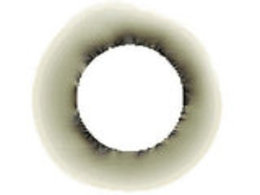
\includegraphics[width=\textwidth,height=\textheight/2,keepaspectratio=true]{intro_wavefunc.jpg}}
\end{DoxyImageNoCaption}


The project was supported ... H\+U\+N\+QT ...

\section*{Dependencies}

The optimization algorithm of Q\+GD relies on the \href{https://www.gnu.org/software/gsl/doc/html/multimin.html}{\tt multimin} component of the \href{https://www.gnu.org/software/gsl/doc/html/index.html}{\tt G\+NU Scientific Library}. We developed and tested the Q\+GD package with G\+NU Scientific Library of version 2.\+5 and 2.\+6. The dependencies necessary to compile and build the Q\+GD package are the followings\+:


\begin{DoxyItemize}
\item \href{https://www.gnu.org/software/automake/}{\tt automake} (for further development purposes)
\item \href{https://www.gnu.org/software/autoconf/}{\tt autoconf} (for further development purposes)
\item \href{https://www.gnu.org/software/libtool/}{\tt libtool}
\item \href{https://www.gnu.org/software/make/}{\tt make}
\item \href{https://www.gnu.org/software/gsl/doc/html/index.html}{\tt G\+NU Scientific Library} ($>$=2.\+5)
\item C++/C \href{https://software.intel.com/content/www/us/en/develop/tools/compilers/c-compilers.html}{\tt Intel} or \href{https://gcc.gnu.org/}{\tt G\+NU} compiler
\item \href{https://software.intel.com/content/www/us/en/develop/tools/math-kernel-library.html}{\tt Intel M\+KL} (optional)
\end{DoxyItemize}

The Python interface of Q\+GD was developed and tested with Python 3.\+6 and 3.\+7. The Q\+GD Python interface needs the following packages to be installed on the system\+:


\begin{DoxyItemize}
\item \href{https://qiskit.org/documentation/install.html}{\tt Qiskit}
\item \href{https://numpy.org/install/}{\tt Numpy}
\item \href{https://www.scipy.org/install.html}{\tt scipy}
\item \href{https://docs.python.org/3/library/ctypes.html}{\tt ctypes}
\end{DoxyItemize}

\section*{How to build G\+NU Scientific Library}

If the G\+NU Scientific Library is not installed on the system, it can be easily compiled and deployed by the end user without administrative privileges. The G\+NU Scientific Library can be downloaded from the site \href{https://www.gnu.org/software/gsl/}{\tt https\+://www.\+gnu.\+org/software/gsl/}. After the downloaded package is extracted somewhere in the home directory of the user ({\bfseries path/to/gslsource}), one should configure the compiling environment using the {\bfseries configure} tool. Depending on the individual settings the default compiler to be invoked might be different from H\+PC to H\+PC. To ensure the usage of the G\+NU compiler, the following shell command should be executed inside the directory {\bfseries path/to/gslsource}\+:

\$ ./configure --prefix=path/to/gsl FC=gfortran CC=gcc C\+XX=g++

(Similarly, Intel compiler can be forced by setting FC=ifort CC=icc and C\+XX=icpc.) The installation directory of the compiled G\+NU Scientific Library is given by --prefix=path/to/gsl (which is different from the directory path of the source files given by {\bfseries path/to/gslsource}). To install G\+NU Scientific Library the user should have read and write permissions on the path {\bfseries path/to/gsl} (which might be for example /home/username/gsl). After the successful configuration the G\+NU Scientific Library can be compiled by the shell command

\$ make

The compilation of the G\+NU Scientific Library takes some time. When the compilation is done, the package (including the C header files and the static and shared libraries) is installed into the directory {\bfseries path/to/gsl} by the shell command\+:

\$ make install

\section*{Download the Quantum Gate Decomposer package}

The developer version Quantum Gate Decomposer package can be downloaded from github repository \href{https://github.com/rakytap/quantum-gate-decomposer/tree/C++}{\tt https\+://github.\+com/rakytap/quantum-\/gate-\/decomposer/tree/\+C++}. After the downloaded package is extracted into the directory {\bfseries path/to/qgdsource} (which would be the path to the source code of the Q\+GD package), one can proceed to the compilation steps described in the next section.

\section*{How to deploy the Quantum Gate Decomposer package}

Similarly to G\+NU Scientific Library, the Q\+GD package is also equipped with automake tools to ease the compilation and the deployment of the package. To ensure that Q\+GD package would find the necessary libraries and header files during compilation time it is advised to define the following environment variables\+:

\$ export G\+S\+L\+\_\+\+L\+I\+B\+\_\+\+D\+IR=path/to/gsl/lib(64)

\$ export G\+S\+L\+\_\+\+I\+N\+C\+\_\+\+D\+IR=path/to/gsl/include

When using Intel compiler equipped with Intel M\+KL on a H\+PC, the compiler can find his way to the M\+KL libraries automatically through the environment variable M\+K\+L\+R\+O\+OT which points to the root directory of the M\+KL package. If the Intel environment variables are not set, they can be initialized by the shell command\+:

\$ source /opt/intel/composerxe/bin/compilervars.sh intel64

where /opt/intel/composerxe is the path to the Intel compiler package location which might be different from the given one. (This step can be omitted when using G\+NU compiler, or when we do not have intention to use Intel M\+KL) After the basic environment variables are set, the compilation can be configured by the command executed in the source directory {\bfseries path/to/qgdsource} of the Q\+GD package\+:

\$ ./configure --prefix=path/to/qgd CC=gcc C\+XX=g++

where path/to/qgd is the installation path of the Quantum Gate Decomposer package. The installation directory of the compiled Q\+GD package is given by --prefix=path/to/qgd (which is different from the directory path of the source files given by {\bfseries path/to/qgdsource}). The user should have read and write permissions on the path {\bfseries path/to/qgd} (which can be for example /home/username/qgd). Another optional flag --enable-\/ffast-\/math enables the compiler\textquotesingle{}s floating-\/point optimization (which is usually enabled by default in Intel compilers settings). While in general this optimization is considered to be dangerous, the runtime performance might be significantly increased due to this optimization. Try to compile without and with this flag and compare the performance and stability of the resulted binaries (for further information see section {\bfseries How to use}). We notice, that the Q\+GD Python interface does not fully support this optimization resulting in lower performance than a standalone C applications. On the other hand, if one choses Intel compiler to built the Q\+GD package, the following configuration settings should be invoked\+:

\$ ./configure --prefix=path/to/qgd --with-\/mkl CC=icc C\+XX=icpc

The --with-\/mkl flag sets the appropriate linking of the Q\+GD package with the Intel M\+KL package. If the flag is missing from the configuration than the C\+B\+L\+AS library of the G\+NU Scientific Library is used for linear algebra operations. After the successful configuration the Q\+GD package can be compiled by the shell command executed in the directory {\bfseries path/to/qgdsource}\+:

\$ make

After a successful compilation of the Q\+GD package, it can be installed into the directory {\bfseries path/to/gsl} by the shell command\+:

\$ make install

The installation procedure will copy all the C header files, the static and shared libraries needed for further developments and the python interface files including a simple python example file {\bfseries \hyperlink{example_8py}{example.\+py}} into the installation destination defined by the {\bfseries path/to$\ast$qgd} path.

\section*{How to use}

The algorithm implemented in the Q\+GD package intends to transform the given unitary into an identity matrix via a sequence of \hyperlink{class_c_n_o_t}{C\+N\+OT} and \hyperlink{class_u3}{U3} operations applied on the unitary. Thus, in order to really get the decomposition of a unitary, one should rather provide the complex transpose of this unitary as the input for the Q\+GD decomposing process.

\subsection*{Standalone executable}

During the compilation and the installation processes of the Q\+GD package a standalone executable was also built and copied into the directory {\bfseries path/to/gsl/bin}. This executable can be executed by a command

\$ ./decomposition\+\_\+test

and it starts a decomposition of a random general unitary matrix. The source of this example is located in {\bfseries path/to/qgdsource/test\+\_\+standalone/} and shows a simple test case of the usage of the Q\+GD package. The Doxygen documentation of the Q\+GD A\+PI can be also generated in order fully exploit the functionalities of the Q\+GD package (for further details see section {\bfseries Doxygen manual} at the end of this manual).

\subsection*{Python Interface}

The Q\+GD package contains a simple python interface allowing the access of the functionalities of the Q\+GD package from Python. The usage of the Q\+GD Python interface is demonstrated in the example file {\bfseries \hyperlink{example_8py}{example.\+py}} located in the directory {\bfseries path/to/qgd} and can be run similarly to any python scripts. The example file imports the {\bfseries \hyperlink{namespaceqgd__python}{qgd\+\_\+python}} module containing the wrapper class for the decomposition of a given unitary matrix. The wrapper class loads the shared library libqgd.\+so and performs the data conversion between the python and C sides.

It should be noted, however, that the python interface functions are implemented only for few functionalities of the whole Q\+GD A\+PI. Another desired interface functions can be implemented following the source of already implemented interface function in source file {\bfseries \hyperlink{python__interface_8cpp}{python\+\_\+interface.\+cpp}} in the main directory of the Q\+GD source code.

\section*{development Development}

The Q\+GD A\+PI enables the extension of the capabilities of the Q\+GD packages into further projects. The Q\+GD header files needed for the compilation of the project are provided in the directory {\bfseries path/to/qgd/include}. The compiled object files should than be linked against the static or shared Q\+GD libraries libqgd.\+a or libqgd.\+so, respectively, located in the directory {\bfseries path/to/qgd/lib(64)}. In order to exploit the speedup comming from the floating point optimization, we notice that Intel\textquotesingle{}s compiler (usually) use this optimization by default, but when linking with G\+NU compiler, the -\/ffast-\/math option must be append when linking against the Q\+GD A\+PI library is done. The full documentation of the Q\+GD A\+PI can be accessed by a Doxygen manual which can be accessed and recreated by steps described in the following section 
\chapter{Module Index}
\section{Modules}
Here is a list of all modules\+:\begin{DoxyCompactList}
\item \contentsline{section}{Examples}{\pageref{group__examples}}{}
\item \contentsline{section}{Frequently asked questions}{\pageref{group__faq}}{}
\item \contentsline{section}{Python Interface}{\pageref{group__python}}{}
\end{DoxyCompactList}

\chapter{Namespace Index}
\section{Namespace List}
Here is a list of all namespaces with brief descriptions\+:\begin{DoxyCompactList}
\item\contentsline{section}{\hyperlink{namespaceexample}{example} }{\pageref{namespaceexample}}{}
\item\contentsline{section}{\hyperlink{namespaceqgd__python}{qgd\+\_\+python} }{\pageref{namespaceqgd__python}}{}
\item\contentsline{section}{\hyperlink{namespaceqgd__python_1_1_n___qubit___decomposition}{qgd\+\_\+python.\+N\+\_\+\+Qubit\+\_\+\+Decomposition} }{\pageref{namespaceqgd__python_1_1_n___qubit___decomposition}}{}
\end{DoxyCompactList}

\chapter{Hierarchical Index}
\section{Class Hierarchy}
This inheritance list is sorted roughly, but not completely, alphabetically\+:\begin{DoxyCompactList}
\item \contentsline{section}{gates\+\_\+num}{\pageref{structgates__num}}{}
\item \contentsline{section}{qgd\+\_\+python.\+N\+\_\+\+Qubit\+\_\+\+Decomposition.\+N\+\_\+\+Qubit\+\_\+\+Decomposition}{\pageref{classqgd__python_1_1_n___qubit___decomposition_1_1_n___qubit___decomposition}}{}
\item \contentsline{section}{Operation}{\pageref{class_operation}}{}
\begin{DoxyCompactList}
\item \contentsline{section}{C\+N\+OT}{\pageref{class_c_n_o_t}}{}
\item \contentsline{section}{C\+N\+OT}{\pageref{class_c_n_o_t}}{}
\item \contentsline{section}{Operation\+\_\+block}{\pageref{class_operation__block}}{}
\begin{DoxyCompactList}
\item \contentsline{section}{Decomposition\+\_\+\+Base}{\pageref{class_decomposition___base}}{}
\begin{DoxyCompactList}
\item \contentsline{section}{N\+\_\+\+Qubit\+\_\+\+Decomposition}{\pageref{class_n___qubit___decomposition}}{}
\item \contentsline{section}{N\+\_\+\+Qubit\+\_\+\+Decomposition}{\pageref{class_n___qubit___decomposition}}{}
\item \contentsline{section}{Sub\+\_\+\+Matrix\+\_\+\+Decomposition}{\pageref{class_sub___matrix___decomposition}}{}
\item \contentsline{section}{Sub\+\_\+\+Matrix\+\_\+\+Decomposition}{\pageref{class_sub___matrix___decomposition}}{}
\item \contentsline{section}{Two\+\_\+\+Qubit\+\_\+\+Decomposition}{\pageref{class_two___qubit___decomposition}}{}
\item \contentsline{section}{Two\+\_\+\+Qubit\+\_\+\+Decomposition}{\pageref{class_two___qubit___decomposition}}{}
\end{DoxyCompactList}
\item \contentsline{section}{Decomposition\+\_\+\+Base}{\pageref{class_decomposition___base}}{}
\end{DoxyCompactList}
\item \contentsline{section}{Operation\+\_\+block}{\pageref{class_operation__block}}{}
\item \contentsline{section}{U3}{\pageref{class_u3}}{}
\item \contentsline{section}{U3}{\pageref{class_u3}}{}
\end{DoxyCompactList}
\item \contentsline{section}{Q\+G\+D\+\_\+\+Complex16}{\pageref{struct_q_g_d___complex16}}{}
\item \contentsline{section}{Random\+\_\+\+Unitary}{\pageref{class_random___unitary}}{}
\end{DoxyCompactList}

\chapter{Class Index}
\section{Class List}
Here are the classes, structs, unions and interfaces with brief descriptions\+:\begin{DoxyCompactList}
\item\contentsline{section}{\hyperlink{class_c_n_o_t}{C\+N\+OT} \\*A class representing a \hyperlink{class_c_n_o_t}{C\+N\+OT} operation }{\pageref{class_c_n_o_t}}{}
\item\contentsline{section}{\hyperlink{class_decomposition___base}{Decomposition\+\_\+\+Base} \\*A class containing basic methods for the decomposition process }{\pageref{class_decomposition___base}}{}
\item\contentsline{section}{\hyperlink{structgates__num}{gates\+\_\+num} \\*Structure type conatining numbers of gates }{\pageref{structgates__num}}{}
\item\contentsline{section}{\hyperlink{class_n___qubit___decomposition}{N\+\_\+\+Qubit\+\_\+\+Decomposition} \\*A class to determine the decomposition of a unitary into a sequence of \hyperlink{class_c_n_o_t}{C\+N\+OT} and \hyperlink{class_u3}{U3} operations }{\pageref{class_n___qubit___decomposition}}{}
\item\contentsline{section}{\hyperlink{classqgd__python_1_1_n___qubit___decomposition_1_1_n___qubit___decomposition}{qgd\+\_\+python.\+N\+\_\+\+Qubit\+\_\+\+Decomposition.\+N\+\_\+\+Qubit\+\_\+\+Decomposition} \\*A class for the decomposition of N-\/qubit unitaries into \hyperlink{class_u3}{U3} and \hyperlink{class_c_n_o_t}{C\+N\+OT} gates }{\pageref{classqgd__python_1_1_n___qubit___decomposition_1_1_n___qubit___decomposition}}{}
\item\contentsline{section}{\hyperlink{class_operation}{Operation} \\*Base class for the representation of one-\/ and two-\/qubit operations }{\pageref{class_operation}}{}
\item\contentsline{section}{\hyperlink{class_operation__block}{Operation\+\_\+block} \\*A class responsible for grouping \hyperlink{class_c_n_o_t}{C\+N\+OT} and \hyperlink{class_u3}{U3} operations into layers }{\pageref{class_operation__block}}{}
\item\contentsline{section}{\hyperlink{struct_q_g_d___complex16}{Q\+G\+D\+\_\+\+Complex16} \\*Structure type representing complex numbers in the Q\+GD package (compatible with cblas libraries) }{\pageref{struct_q_g_d___complex16}}{}
\item\contentsline{section}{\hyperlink{class_random___unitary}{Random\+\_\+\+Unitary} }{\pageref{class_random___unitary}}{}
\item\contentsline{section}{\hyperlink{class_sub___matrix___decomposition}{Sub\+\_\+\+Matrix\+\_\+\+Decomposition} \\*A class responsible for the disentanglement of one qubit from the others }{\pageref{class_sub___matrix___decomposition}}{}
\item\contentsline{section}{\hyperlink{class_two___qubit___decomposition}{Two\+\_\+\+Qubit\+\_\+\+Decomposition} }{\pageref{class_two___qubit___decomposition}}{}
\item\contentsline{section}{\hyperlink{class_u3}{U3} \\*A class representing a \hyperlink{class_u3}{U3} operation }{\pageref{class_u3}}{}
\end{DoxyCompactList}

\chapter{File Index}
\section{File List}
Here is a list of all files with brief descriptions\+:\begin{DoxyCompactList}
\item\contentsline{section}{\hyperlink{____init_____8py}{\+\_\+\+\_\+init\+\_\+\+\_\+.\+py} }{\pageref{____init_____8py}}{}
\item\contentsline{section}{\hyperlink{_c_n_o_t_8cpp}{C\+N\+O\+T.\+cpp} }{\pageref{_c_n_o_t_8cpp}}{}
\item\contentsline{section}{\hyperlink{operations_2include_2_c_n_o_t_8h}{operations/include/\+C\+N\+O\+T.\+h} }{\pageref{operations_2include_2_c_n_o_t_8h}}{}
\item\contentsline{section}{\hyperlink{qgd_2_c_n_o_t_8h}{qgd/\+C\+N\+O\+T.\+h} }{\pageref{qgd_2_c_n_o_t_8h}}{}
\item\contentsline{section}{\hyperlink{common_8cpp}{common.\+cpp} }{\pageref{common_8cpp}}{}
\item\contentsline{section}{\hyperlink{common_2include_2common_8h}{common/include/common.\+h} }{\pageref{common_2include_2common_8h}}{}
\item\contentsline{section}{\hyperlink{qgd_2common_8h}{qgd/common.\+h} }{\pageref{qgd_2common_8h}}{}
\item\contentsline{section}{\hyperlink{_decomposition___base_8cpp}{Decomposition\+\_\+\+Base.\+cpp} }{\pageref{_decomposition___base_8cpp}}{}
\item\contentsline{section}{\hyperlink{decomposition_2include_2_decomposition___base_8h}{decomposition/include/\+Decomposition\+\_\+\+Base.\+h} }{\pageref{decomposition_2include_2_decomposition___base_8h}}{}
\item\contentsline{section}{\hyperlink{qgd_2_decomposition___base_8h}{qgd/\+Decomposition\+\_\+\+Base.\+h} }{\pageref{qgd_2_decomposition___base_8h}}{}
\item\contentsline{section}{\hyperlink{decomposition__test_8cpp}{decomposition\+\_\+test.\+cpp} }{\pageref{decomposition__test_8cpp}}{}
\item\contentsline{section}{\hyperlink{standalone_2decomposition__test_8cpp}{standalone/decomposition\+\_\+test.\+cpp} }{\pageref{standalone_2decomposition__test_8cpp}}{}
\item\contentsline{section}{\hyperlink{example_8py}{example.\+py} }{\pageref{example_8py}}{}
\item\contentsline{section}{\hyperlink{_n___qubit___decomposition_8cpp}{N\+\_\+\+Qubit\+\_\+\+Decomposition.\+cpp} }{\pageref{_n___qubit___decomposition_8cpp}}{}
\item\contentsline{section}{\hyperlink{decomposition_2include_2_n___qubit___decomposition_8h}{decomposition/include/\+N\+\_\+\+Qubit\+\_\+\+Decomposition.\+h} }{\pageref{decomposition_2include_2_n___qubit___decomposition_8h}}{}
\item\contentsline{section}{\hyperlink{qgd_2_n___qubit___decomposition_8h}{qgd/\+N\+\_\+\+Qubit\+\_\+\+Decomposition.\+h} }{\pageref{qgd_2_n___qubit___decomposition_8h}}{}
\item\contentsline{section}{\hyperlink{_n___qubit___decomposition_8py}{N\+\_\+\+Qubit\+\_\+\+Decomposition.\+py} }{\pageref{_n___qubit___decomposition_8py}}{}
\item\contentsline{section}{\hyperlink{_operation_8cpp}{Operation.\+cpp} }{\pageref{_operation_8cpp}}{}
\item\contentsline{section}{\hyperlink{operations_2include_2_operation_8h}{operations/include/\+Operation.\+h} }{\pageref{operations_2include_2_operation_8h}}{}
\item\contentsline{section}{\hyperlink{qgd_2_operation_8h}{qgd/\+Operation.\+h} }{\pageref{qgd_2_operation_8h}}{}
\item\contentsline{section}{\hyperlink{_operation__block_8cpp}{Operation\+\_\+block.\+cpp} }{\pageref{_operation__block_8cpp}}{}
\item\contentsline{section}{\hyperlink{operations_2include_2_operation__block_8h}{operations/include/\+Operation\+\_\+block.\+h} }{\pageref{operations_2include_2_operation__block_8h}}{}
\item\contentsline{section}{\hyperlink{qgd_2_operation__block_8h}{qgd/\+Operation\+\_\+block.\+h} }{\pageref{qgd_2_operation__block_8h}}{}
\item\contentsline{section}{\hyperlink{operation__test_8cpp}{operation\+\_\+test.\+cpp} }{\pageref{operation__test_8cpp}}{}
\item\contentsline{section}{\hyperlink{python__interface_8cpp}{python\+\_\+interface.\+cpp} }{\pageref{python__interface_8cpp}}{}
\item\contentsline{section}{\hyperlink{python__interface_8h}{python\+\_\+interface.\+h} }{\pageref{python__interface_8h}}{}
\item\contentsline{section}{\hyperlink{qgd_2python__interface_8h}{qgd/python\+\_\+interface.\+h} }{\pageref{qgd_2python__interface_8h}}{}
\item\contentsline{section}{\hyperlink{_random___unitary_8cpp}{Random\+\_\+\+Unitary.\+cpp} }{\pageref{_random___unitary_8cpp}}{}
\item\contentsline{section}{\hyperlink{qgd_2_random___unitary_8h}{qgd/\+Random\+\_\+\+Unitary.\+h} }{\pageref{qgd_2_random___unitary_8h}}{}
\item\contentsline{section}{\hyperlink{random__unitary_2include_2_random___unitary_8h}{random\+\_\+unitary/include/\+Random\+\_\+\+Unitary.\+h} }{\pageref{random__unitary_2include_2_random___unitary_8h}}{}
\item\contentsline{section}{\hyperlink{_sub___matrix___decomposition_8cpp}{Sub\+\_\+\+Matrix\+\_\+\+Decomposition.\+cpp} }{\pageref{_sub___matrix___decomposition_8cpp}}{}
\item\contentsline{section}{\hyperlink{decomposition_2include_2_sub___matrix___decomposition_8h}{decomposition/include/\+Sub\+\_\+\+Matrix\+\_\+\+Decomposition.\+h} }{\pageref{decomposition_2include_2_sub___matrix___decomposition_8h}}{}
\item\contentsline{section}{\hyperlink{qgd_2_sub___matrix___decomposition_8h}{qgd/\+Sub\+\_\+\+Matrix\+\_\+\+Decomposition.\+h} }{\pageref{qgd_2_sub___matrix___decomposition_8h}}{}
\item\contentsline{section}{\hyperlink{decomposition_2include_2_two___qubit___decomposition_8h}{decomposition/include/\+Two\+\_\+\+Qubit\+\_\+\+Decomposition.\+h} }{\pageref{decomposition_2include_2_two___qubit___decomposition_8h}}{}
\item\contentsline{section}{\hyperlink{qgd_2_two___qubit___decomposition_8h}{qgd/\+Two\+\_\+\+Qubit\+\_\+\+Decomposition.\+h} }{\pageref{qgd_2_two___qubit___decomposition_8h}}{}
\item\contentsline{section}{\hyperlink{_u3_8cpp}{U3.\+cpp} }{\pageref{_u3_8cpp}}{}
\item\contentsline{section}{\hyperlink{operations_2include_2_u3_8h}{operations/include/\+U3.\+h} }{\pageref{operations_2include_2_u3_8h}}{}
\item\contentsline{section}{\hyperlink{qgd_2_u3_8h}{qgd/\+U3.\+h} }{\pageref{qgd_2_u3_8h}}{}
\end{DoxyCompactList}

\chapter{Module Documentation}
\hypertarget{group__examples}{}\section{Examples}
\label{group__examples}\index{Examples@{Examples}}
ghtrhjtr 
\hypertarget{group__faq}{}\section{Frequently asked questions}
\label{group__faq}\index{Frequently asked questions@{Frequently asked questions}}
ghtrhjtr 
\hypertarget{group__python}{}\section{Python Interface}
\label{group__python}\index{Python Interface@{Python Interface}}


$\ast$$\ast$$\ast$$\ast$$\ast$$\ast$$\ast$$\ast$$\ast$$\ast$$\ast$\+M\+O\+O\+O\+O\+O\+O\+O\+O\+O\+R\+R\+R\+R\+R\+R\+E\+E\+E\+E\+E\+E\+E\+E\+E\+E\+E\+E\+EE D\+E\+E\+E\+E\+E\+E\+E\+E\+E\+E\+E\+E\+E\+T\+A\+A\+A\+A\+A\+A\+A\+A\+A\+A\+A\+A\+A\+A\+A\+A\+I\+L\+S\+S\+S\+S\+S\+S\+S\+S\+S\+S\+S\+S\+SS H\+E\+E\+E\+E\+E\+E\+E\+E\+E\+E\+E\+E\+E\+E\+R\+E\+E\+E\+E\+E\+E\+E\+E\+E\+EE $\ast$$\ast$$\ast$$\ast$$\ast$$\ast$$\ast$$\ast$$\ast$$\ast$$\ast$$\ast$$\ast$$\ast$$\ast$$\ast$  


\subsection*{Classes}
\begin{DoxyCompactItemize}
\item 
class \hyperlink{classqgd__python_1_1_n___qubit___decomposition_1_1_n___qubit___decomposition}{qgd\+\_\+python.\+N\+\_\+\+Qubit\+\_\+\+Decomposition.\+N\+\_\+\+Qubit\+\_\+\+Decomposition}
\begin{DoxyCompactList}\small\item\em A class for the decomposition of N-\/qubit unitaries into \hyperlink{class_u3}{U3} and \hyperlink{class_c_n_o_t}{C\+N\+OT} gates. \end{DoxyCompactList}\end{DoxyCompactItemize}
\subsection*{Functions}
\begin{DoxyCompactItemize}
\item 
def \hyperlink{group__python_gaeba96037339a2173be32f9da54b2b640}{qgd\+\_\+python.\+N\+\_\+\+Qubit\+\_\+\+Decomposition.\+\_\+\+\_\+del\+\_\+\+\_\+} (self)
\begin{DoxyCompactList}\small\item\em Destructor of the class. \end{DoxyCompactList}\item 
def \hyperlink{group__python_gaa61a063ce130eec9f91483ea366c4875}{qgd\+\_\+python.\+N\+\_\+\+Qubit\+\_\+\+Decomposition.\+\_\+\+\_\+init\+\_\+\+\_\+} (self, Umtx, optimize\+\_\+layer\+\_\+num=False, initial\+\_\+guess=\char`\"{}zeros\char`\"{})
\begin{DoxyCompactList}\small\item\em Constructor of the class. \end{DoxyCompactList}\item 
def \hyperlink{group__python_ga7f84dd22a6748be01c990c734e95c23d}{qgd\+\_\+python.\+N\+\_\+\+Qubit\+\_\+\+Decomposition.\+get\+\_\+quantum\+\_\+circuit} (self)
\begin{DoxyCompactList}\small\item\em Export the unitary decomposition into Qiskit format. \end{DoxyCompactList}\item 
def \hyperlink{group__python_ga90a4aa2757be84217c83aad59a5baf60}{qgd\+\_\+python.\+N\+\_\+\+Qubit\+\_\+\+Decomposition.\+list\+\_\+operations} (self, start\+\_\+index=1)
\begin{DoxyCompactList}\small\item\em Lists the operations decomposing the initial unitary. \end{DoxyCompactList}\item 
def \hyperlink{group__python_ga0b1a2119452bd55192ed3e49450030aa}{qgd\+\_\+python.\+N\+\_\+\+Qubit\+\_\+\+Decomposition.\+set\+\_\+identical\+\_\+blocks} (self, qbit, identical\+\_\+blocks)
\begin{DoxyCompactList}\small\item\em Set the number of identical successive blocks during the subdecomposition of the qbit-\/th qubit. \end{DoxyCompactList}\item 
def \hyperlink{group__python_ga5c703393d528f31a2d1aa2cc7282c691}{qgd\+\_\+python.\+N\+\_\+\+Qubit\+\_\+\+Decomposition.\+set\+\_\+iteration\+\_\+loops} (self, qbit, iteration\+\_\+loops)
\begin{DoxyCompactList}\small\item\em Set the number of iteration loops during the subdecomposition of the qbit-\/th qubit. \end{DoxyCompactList}\item 
def \hyperlink{group__python_ga194ae83da0f906220e3b001d1bac14bc}{qgd\+\_\+python.\+N\+\_\+\+Qubit\+\_\+\+Decomposition.\+set\+\_\+max\+\_\+layer\+\_\+num} (self, qbit, max\+\_\+layer\+\_\+num)
\begin{DoxyCompactList}\small\item\em Set the maximal number of layers used in the subdecomposition of the qbit-\/th qubit. \end{DoxyCompactList}\item 
def \hyperlink{group__python_ga0001a3a473bd31784f1da0d018a7529a}{qgd\+\_\+python.\+N\+\_\+\+Qubit\+\_\+\+Decomposition.\+start\+\_\+decomposition} (self, finalize\+\_\+decomposition=True)
\begin{DoxyCompactList}\small\item\em Start the disentanglig process of the least significant two qubit unitary. \end{DoxyCompactList}\end{DoxyCompactItemize}
\subsection*{Variables}
\begin{DoxyCompactItemize}
\item 
\hyperlink{group__python_gaab3ee0c640088387c37d0bea14b0bbd0}{qgd\+\_\+python.\+N\+\_\+\+Qubit\+\_\+\+Decomposition.\+\_\+qgd\+\_\+library} = ctypes.\+cdll.\+Load\+Library(library\+\_\+path)
\item 
\hyperlink{group__python_gacb3a3a21bbd6fbe8c612122ea586f1e9}{qgd\+\_\+python.\+N\+\_\+\+Qubit\+\_\+\+Decomposition.\+argtypes}
\item 
string \hyperlink{group__python_ga36e466ce872adb198d01ce19abdd3177}{qgd\+\_\+python.\+N\+\_\+\+Qubit\+\_\+\+Decomposition.\+library\+\_\+path} = \textquotesingle{}.libs/libqgd.\+so\textquotesingle{}
\item 
\hyperlink{group__python_ga9341b826d33e46599c99a2da15e9c2be}{qgd\+\_\+python.\+N\+\_\+\+Qubit\+\_\+\+Decomposition.\+restype}
\end{DoxyCompactItemize}


\subsection{Detailed Description}
$\ast$$\ast$$\ast$$\ast$$\ast$$\ast$$\ast$$\ast$$\ast$$\ast$$\ast$\+M\+O\+O\+O\+O\+O\+O\+O\+O\+O\+R\+R\+R\+R\+R\+R\+E\+E\+E\+E\+E\+E\+E\+E\+E\+E\+E\+E\+EE D\+E\+E\+E\+E\+E\+E\+E\+E\+E\+E\+E\+E\+E\+T\+A\+A\+A\+A\+A\+A\+A\+A\+A\+A\+A\+A\+A\+A\+A\+A\+I\+L\+S\+S\+S\+S\+S\+S\+S\+S\+S\+S\+S\+S\+SS H\+E\+E\+E\+E\+E\+E\+E\+E\+E\+E\+E\+E\+E\+E\+R\+E\+E\+E\+E\+E\+E\+E\+E\+E\+EE $\ast$$\ast$$\ast$$\ast$$\ast$$\ast$$\ast$$\ast$$\ast$$\ast$$\ast$$\ast$$\ast$$\ast$$\ast$$\ast$ 



\subsection{Function Documentation}
\index{Python Interface@{Python Interface}!\+\_\+\+\_\+del\+\_\+\+\_\+@{\+\_\+\+\_\+del\+\_\+\+\_\+}}
\index{\+\_\+\+\_\+del\+\_\+\+\_\+@{\+\_\+\+\_\+del\+\_\+\+\_\+}!Python Interface@{Python Interface}}
\subsubsection[{\texorpdfstring{\+\_\+\+\_\+del\+\_\+\+\_\+(self)}{__del__(self)}}]{\setlength{\rightskip}{0pt plus 5cm}def qgd\+\_\+python.\+N\+\_\+\+Qubit\+\_\+\+Decomposition.\+\_\+\+\_\+del\+\_\+\+\_\+ (
\begin{DoxyParamCaption}
\item[{}]{self}
\end{DoxyParamCaption}
)}\hypertarget{group__python_gaeba96037339a2173be32f9da54b2b640}{}\label{group__python_gaeba96037339a2173be32f9da54b2b640}


Destructor of the class. 



Definition at line 109 of file N\+\_\+\+Qubit\+\_\+\+Decomposition.\+py.

\index{Python Interface@{Python Interface}!\+\_\+\+\_\+init\+\_\+\+\_\+@{\+\_\+\+\_\+init\+\_\+\+\_\+}}
\index{\+\_\+\+\_\+init\+\_\+\+\_\+@{\+\_\+\+\_\+init\+\_\+\+\_\+}!Python Interface@{Python Interface}}
\subsubsection[{\texorpdfstring{\+\_\+\+\_\+init\+\_\+\+\_\+(self, Umtx, optimize\+\_\+layer\+\_\+num=\+False, initial\+\_\+guess=""zeros"")}{__init__(self, Umtx, optimize_layer_num=False, initial_guess="zeros")}}]{\setlength{\rightskip}{0pt plus 5cm}def qgd\+\_\+python.\+N\+\_\+\+Qubit\+\_\+\+Decomposition.\+\_\+\+\_\+init\+\_\+\+\_\+ (
\begin{DoxyParamCaption}
\item[{}]{self, }
\item[{}]{Umtx, }
\item[{}]{optimize\+\_\+layer\+\_\+num = {\ttfamily False}, }
\item[{}]{initial\+\_\+guess = {\ttfamily \char`\"{}zeros\char`\"{}}}
\end{DoxyParamCaption}
)}\hypertarget{group__python_gaa61a063ce130eec9f91483ea366c4875}{}\label{group__python_gaa61a063ce130eec9f91483ea366c4875}


Constructor of the class. 


\begin{DoxyParams}{Parameters}
{\em Umtx} & The unitary matrix \\
\hline
{\em initial\+\_\+guess} & \\
\hline
\end{DoxyParams}
\begin{DoxyReturn}{Returns}
An instance of the class 
\end{DoxyReturn}


Definition at line 77 of file N\+\_\+\+Qubit\+\_\+\+Decomposition.\+py.

\index{Python Interface@{Python Interface}!get\+\_\+quantum\+\_\+circuit@{get\+\_\+quantum\+\_\+circuit}}
\index{get\+\_\+quantum\+\_\+circuit@{get\+\_\+quantum\+\_\+circuit}!Python Interface@{Python Interface}}
\subsubsection[{\texorpdfstring{get\+\_\+quantum\+\_\+circuit(self)}{get_quantum_circuit(self)}}]{\setlength{\rightskip}{0pt plus 5cm}def qgd\+\_\+python.\+N\+\_\+\+Qubit\+\_\+\+Decomposition.\+get\+\_\+quantum\+\_\+circuit (
\begin{DoxyParamCaption}
\item[{}]{self}
\end{DoxyParamCaption}
)}\hypertarget{group__python_ga7f84dd22a6748be01c990c734e95c23d}{}\label{group__python_ga7f84dd22a6748be01c990c734e95c23d}


Export the unitary decomposition into Qiskit format. 


\begin{DoxyParams}{Parameters}
{\em start\+\_\+index} & The index of the first inverse operation \\
\hline
\end{DoxyParams}


Definition at line 166 of file N\+\_\+\+Qubit\+\_\+\+Decomposition.\+py.

\index{Python Interface@{Python Interface}!list\+\_\+operations@{list\+\_\+operations}}
\index{list\+\_\+operations@{list\+\_\+operations}!Python Interface@{Python Interface}}
\subsubsection[{\texorpdfstring{list\+\_\+operations(self, start\+\_\+index=1)}{list_operations(self, start_index=1)}}]{\setlength{\rightskip}{0pt plus 5cm}def qgd\+\_\+python.\+N\+\_\+\+Qubit\+\_\+\+Decomposition.\+list\+\_\+operations (
\begin{DoxyParamCaption}
\item[{}]{self, }
\item[{}]{start\+\_\+index = {\ttfamily 1}}
\end{DoxyParamCaption}
)}\hypertarget{group__python_ga90a4aa2757be84217c83aad59a5baf60}{}\label{group__python_ga90a4aa2757be84217c83aad59a5baf60}


Lists the operations decomposing the initial unitary. 

(These operations are the inverse operations of the operations bringing the intial matrix into unity.) 
\begin{DoxyParams}{Parameters}
{\em start\+\_\+index} & The index of the first inverse operation \\
\hline
\end{DoxyParams}


Definition at line 158 of file N\+\_\+\+Qubit\+\_\+\+Decomposition.\+py.

\index{Python Interface@{Python Interface}!set\+\_\+identical\+\_\+blocks@{set\+\_\+identical\+\_\+blocks}}
\index{set\+\_\+identical\+\_\+blocks@{set\+\_\+identical\+\_\+blocks}!Python Interface@{Python Interface}}
\subsubsection[{\texorpdfstring{set\+\_\+identical\+\_\+blocks(self, qbit, identical\+\_\+blocks)}{set_identical_blocks(self, qbit, identical_blocks)}}]{\setlength{\rightskip}{0pt plus 5cm}def qgd\+\_\+python.\+N\+\_\+\+Qubit\+\_\+\+Decomposition.\+set\+\_\+identical\+\_\+blocks (
\begin{DoxyParamCaption}
\item[{}]{self, }
\item[{}]{qbit, }
\item[{}]{identical\+\_\+blocks}
\end{DoxyParamCaption}
)}\hypertarget{group__python_ga0b1a2119452bd55192ed3e49450030aa}{}\label{group__python_ga0b1a2119452bd55192ed3e49450030aa}


Set the number of identical successive blocks during the subdecomposition of the qbit-\/th qubit. 


\begin{DoxyParams}{Parameters}
{\em qbit} & The number of qubits for which the maximal number of layers should be used in the subdecomposition. \\
\hline
{\em identical\+\_\+blocks} & The number of successive identical layers used in the subdecomposition. \\
\hline
\end{DoxyParams}


Definition at line 149 of file N\+\_\+\+Qubit\+\_\+\+Decomposition.\+py.

\index{Python Interface@{Python Interface}!set\+\_\+iteration\+\_\+loops@{set\+\_\+iteration\+\_\+loops}}
\index{set\+\_\+iteration\+\_\+loops@{set\+\_\+iteration\+\_\+loops}!Python Interface@{Python Interface}}
\subsubsection[{\texorpdfstring{set\+\_\+iteration\+\_\+loops(self, qbit, iteration\+\_\+loops)}{set_iteration_loops(self, qbit, iteration_loops)}}]{\setlength{\rightskip}{0pt plus 5cm}def qgd\+\_\+python.\+N\+\_\+\+Qubit\+\_\+\+Decomposition.\+set\+\_\+iteration\+\_\+loops (
\begin{DoxyParamCaption}
\item[{}]{self, }
\item[{}]{qbit, }
\item[{}]{iteration\+\_\+loops}
\end{DoxyParamCaption}
)}\hypertarget{group__python_ga5c703393d528f31a2d1aa2cc7282c691}{}\label{group__python_ga5c703393d528f31a2d1aa2cc7282c691}


Set the number of iteration loops during the subdecomposition of the qbit-\/th qubit. 


\begin{DoxyParams}{Parameters}
{\em qbit} & The number of qubits for which the maximal number of layers should be used in the subdecomposition., \\
\hline
{\em iteration\+\_\+loops} & The number of iteration loops in each sted of the subdecomposition. \\
\hline
\end{DoxyParams}


Definition at line 139 of file N\+\_\+\+Qubit\+\_\+\+Decomposition.\+py.

\index{Python Interface@{Python Interface}!set\+\_\+max\+\_\+layer\+\_\+num@{set\+\_\+max\+\_\+layer\+\_\+num}}
\index{set\+\_\+max\+\_\+layer\+\_\+num@{set\+\_\+max\+\_\+layer\+\_\+num}!Python Interface@{Python Interface}}
\subsubsection[{\texorpdfstring{set\+\_\+max\+\_\+layer\+\_\+num(self, qbit, max\+\_\+layer\+\_\+num)}{set_max_layer_num(self, qbit, max_layer_num)}}]{\setlength{\rightskip}{0pt plus 5cm}def qgd\+\_\+python.\+N\+\_\+\+Qubit\+\_\+\+Decomposition.\+set\+\_\+max\+\_\+layer\+\_\+num (
\begin{DoxyParamCaption}
\item[{}]{self, }
\item[{}]{qbit, }
\item[{}]{max\+\_\+layer\+\_\+num}
\end{DoxyParamCaption}
)}\hypertarget{group__python_ga194ae83da0f906220e3b001d1bac14bc}{}\label{group__python_ga194ae83da0f906220e3b001d1bac14bc}


Set the maximal number of layers used in the subdecomposition of the qbit-\/th qubit. 


\begin{DoxyParams}{Parameters}
{\em qbit} & The number of qubits for which the maximal number of layers should be used in the subdecomposition. \\
\hline
{\em max\+\_\+layer\+\_\+num} & The maximal number of the operation layers used in the subdecomposition. \\
\hline
\end{DoxyParams}


Definition at line 130 of file N\+\_\+\+Qubit\+\_\+\+Decomposition.\+py.

\index{Python Interface@{Python Interface}!start\+\_\+decomposition@{start\+\_\+decomposition}}
\index{start\+\_\+decomposition@{start\+\_\+decomposition}!Python Interface@{Python Interface}}
\subsubsection[{\texorpdfstring{start\+\_\+decomposition(self, finalize\+\_\+decomposition=\+True)}{start_decomposition(self, finalize_decomposition=True)}}]{\setlength{\rightskip}{0pt plus 5cm}def qgd\+\_\+python.\+N\+\_\+\+Qubit\+\_\+\+Decomposition.\+start\+\_\+decomposition (
\begin{DoxyParamCaption}
\item[{}]{self, }
\item[{}]{finalize\+\_\+decomposition = {\ttfamily True}}
\end{DoxyParamCaption}
)}\hypertarget{group__python_ga0001a3a473bd31784f1da0d018a7529a}{}\label{group__python_ga0001a3a473bd31784f1da0d018a7529a}


Start the disentanglig process of the least significant two qubit unitary. 


\begin{DoxyParams}{Parameters}
{\em finalize\+\_\+decomposition} & Optional logical parameter. If true (default), the decoupled qubits are rotated into state $\vert$0$>$ when the disentangling of the qubits is done. Set to False to omit this procedure \\
\hline
\end{DoxyParams}


Definition at line 120 of file N\+\_\+\+Qubit\+\_\+\+Decomposition.\+py.



\subsection{Variable Documentation}
\index{Python Interface@{Python Interface}!\+\_\+qgd\+\_\+library@{\+\_\+qgd\+\_\+library}}
\index{\+\_\+qgd\+\_\+library@{\+\_\+qgd\+\_\+library}!Python Interface@{Python Interface}}
\subsubsection[{\texorpdfstring{\+\_\+qgd\+\_\+library}{_qgd_library}}]{\setlength{\rightskip}{0pt plus 5cm}qgd\+\_\+python.\+N\+\_\+\+Qubit\+\_\+\+Decomposition.\+\_\+qgd\+\_\+library = ctypes.\+cdll.\+Load\+Library(library\+\_\+path)\hspace{0.3cm}{\ttfamily [private]}}\hypertarget{group__python_gaab3ee0c640088387c37d0bea14b0bbd0}{}\label{group__python_gaab3ee0c640088387c37d0bea14b0bbd0}


Definition at line 47 of file N\+\_\+\+Qubit\+\_\+\+Decomposition.\+py.

\index{Python Interface@{Python Interface}!argtypes@{argtypes}}
\index{argtypes@{argtypes}!Python Interface@{Python Interface}}
\subsubsection[{\texorpdfstring{argtypes}{argtypes}}]{\setlength{\rightskip}{0pt plus 5cm}qgd\+\_\+python.\+N\+\_\+\+Qubit\+\_\+\+Decomposition.\+argtypes}\hypertarget{group__python_gacb3a3a21bbd6fbe8c612122ea586f1e9}{}\label{group__python_gacb3a3a21bbd6fbe8c612122ea586f1e9}


Definition at line 53 of file N\+\_\+\+Qubit\+\_\+\+Decomposition.\+py.

\index{Python Interface@{Python Interface}!library\+\_\+path@{library\+\_\+path}}
\index{library\+\_\+path@{library\+\_\+path}!Python Interface@{Python Interface}}
\subsubsection[{\texorpdfstring{library\+\_\+path}{library_path}}]{\setlength{\rightskip}{0pt plus 5cm}string qgd\+\_\+python.\+N\+\_\+\+Qubit\+\_\+\+Decomposition.\+library\+\_\+path = \textquotesingle{}.libs/libqgd.\+so\textquotesingle{}}\hypertarget{group__python_ga36e466ce872adb198d01ce19abdd3177}{}\label{group__python_ga36e466ce872adb198d01ce19abdd3177}


Definition at line 38 of file N\+\_\+\+Qubit\+\_\+\+Decomposition.\+py.

\index{Python Interface@{Python Interface}!restype@{restype}}
\index{restype@{restype}!Python Interface@{Python Interface}}
\subsubsection[{\texorpdfstring{restype}{restype}}]{\setlength{\rightskip}{0pt plus 5cm}qgd\+\_\+python.\+N\+\_\+\+Qubit\+\_\+\+Decomposition.\+restype}\hypertarget{group__python_ga9341b826d33e46599c99a2da15e9c2be}{}\label{group__python_ga9341b826d33e46599c99a2da15e9c2be}


Definition at line 54 of file N\+\_\+\+Qubit\+\_\+\+Decomposition.\+py.


\chapter{Namespace Documentation}
\hypertarget{namespaceexample}{}\section{example Namespace Reference}
\label{namespaceexample}\index{example@{example}}
\subsection*{Variables}
\begin{DoxyCompactItemize}
\item 
\hyperlink{namespaceexample_a6b87ddad36fca2722dc5fd955536f578}{backend} = Aer.\+get\+\_\+backend(\textquotesingle{}unitary\+\_\+simulator\textquotesingle{})
\item 
\hyperlink{namespaceexample_a0a2e936f47382b2bd8c9432ca77c6026}{c\+Decompose} = \hyperlink{classqgd__python_1_1_n___qubit___decomposition_1_1_n___qubit___decomposition}{N\+\_\+\+Qubit\+\_\+\+Decomposition}( Umtx.\+conj().T )
\item 
\hyperlink{namespaceexample_a9b062b4feb0fe50b0056ed5abb65681c}{data} = loadmat(\textquotesingle{}Umtx.\+mat\textquotesingle{})
\item 
\hyperlink{namespaceexample_a4373e9d1485c7c940b9360eb187bca34}{decomposed\+\_\+matrix} = result.\+get\+\_\+unitary(\hyperlink{namespaceexample_a1602c6a1a270f94e2c254b3b6501cd86}{quantum\+\_\+circuit})
\item 
\hyperlink{namespaceexample_af790bb908348ee47307d4eb3668aa5a0}{decomposition\+\_\+error} = L\+A.\+norm(\hyperlink{namespaceexample_ac1039984599e8ffdf0b609b0e2790c1a}{product\+\_\+matrix} -\/ np.\+identity(16)$\ast$\hyperlink{namespaceexample_ac1039984599e8ffdf0b609b0e2790c1a}{product\+\_\+matrix}\mbox{[}0,0\mbox{]}, 2)
\item 
\hyperlink{namespaceexample_acc723d25fd7224c46ee94d2866c9f96a}{job} = execute(\hyperlink{namespaceexample_a1602c6a1a270f94e2c254b3b6501cd86}{quantum\+\_\+circuit}, \hyperlink{namespaceexample_a6b87ddad36fca2722dc5fd955536f578}{backend})
\item 
\hyperlink{namespaceexample_ae04701779f635cdceb8bdee5c8ff074f}{matrix\+\_\+size} = int(2$\ast$$\ast$\hyperlink{namespaceexample_aedf2ea7d5e512f6db84a19d73dbd5305}{qbit\+\_\+num})
\item 
\hyperlink{namespaceexample_ac1039984599e8ffdf0b609b0e2790c1a}{product\+\_\+matrix} = np.\+dot(\hyperlink{namespaceexample_a9f6bbbedb3a0154f9a0199a632198b9f}{Umtx}, decomposed\+\_\+matrix.\+conj().T)
\item 
int \hyperlink{namespaceexample_aedf2ea7d5e512f6db84a19d73dbd5305}{qbit\+\_\+num} = 3
\item 
\hyperlink{namespaceexample_a1602c6a1a270f94e2c254b3b6501cd86}{quantum\+\_\+circuit} = c\+Decompose.\+get\+\_\+quantum\+\_\+circuit()
\item 
\hyperlink{namespaceexample_ae9f7cf9f0786fe88c5590ca4ad5a295a}{result} = job.\+result()
\item 
\hyperlink{namespaceexample_a9f6bbbedb3a0154f9a0199a632198b9f}{Umtx} = unitary\+\_\+group.\+rvs(\hyperlink{namespaceexample_ae04701779f635cdceb8bdee5c8ff074f}{matrix\+\_\+size})
\end{DoxyCompactItemize}


\subsection{Variable Documentation}
\index{example@{example}!backend@{backend}}
\index{backend@{backend}!example@{example}}
\subsubsection[{\texorpdfstring{backend}{backend}}]{\setlength{\rightskip}{0pt plus 5cm}example.\+backend = Aer.\+get\+\_\+backend(\textquotesingle{}unitary\+\_\+simulator\textquotesingle{})}\hypertarget{namespaceexample_a6b87ddad36fca2722dc5fd955536f578}{}\label{namespaceexample_a6b87ddad36fca2722dc5fd955536f578}


Definition at line 111 of file example.\+py.

\index{example@{example}!c\+Decompose@{c\+Decompose}}
\index{c\+Decompose@{c\+Decompose}!example@{example}}
\subsubsection[{\texorpdfstring{c\+Decompose}{cDecompose}}]{\setlength{\rightskip}{0pt plus 5cm}example.\+c\+Decompose = {\bf N\+\_\+\+Qubit\+\_\+\+Decomposition}( Umtx.\+conj().T )}\hypertarget{namespaceexample_a0a2e936f47382b2bd8c9432ca77c6026}{}\label{namespaceexample_a0a2e936f47382b2bd8c9432ca77c6026}


Definition at line 44 of file example.\+py.

\index{example@{example}!data@{data}}
\index{data@{data}!example@{example}}
\subsubsection[{\texorpdfstring{data}{data}}]{\setlength{\rightskip}{0pt plus 5cm}example.\+data = loadmat(\textquotesingle{}Umtx.\+mat\textquotesingle{})}\hypertarget{namespaceexample_a9b062b4feb0fe50b0056ed5abb65681c}{}\label{namespaceexample_a9b062b4feb0fe50b0056ed5abb65681c}


Definition at line 67 of file example.\+py.

\index{example@{example}!decomposed\+\_\+matrix@{decomposed\+\_\+matrix}}
\index{decomposed\+\_\+matrix@{decomposed\+\_\+matrix}!example@{example}}
\subsubsection[{\texorpdfstring{decomposed\+\_\+matrix}{decomposed_matrix}}]{\setlength{\rightskip}{0pt plus 5cm}example.\+decomposed\+\_\+matrix = result.\+get\+\_\+unitary({\bf quantum\+\_\+circuit})}\hypertarget{namespaceexample_a4373e9d1485c7c940b9360eb187bca34}{}\label{namespaceexample_a4373e9d1485c7c940b9360eb187bca34}


Definition at line 118 of file example.\+py.

\index{example@{example}!decomposition\+\_\+error@{decomposition\+\_\+error}}
\index{decomposition\+\_\+error@{decomposition\+\_\+error}!example@{example}}
\subsubsection[{\texorpdfstring{decomposition\+\_\+error}{decomposition_error}}]{\setlength{\rightskip}{0pt plus 5cm}example.\+decomposition\+\_\+error = L\+A.\+norm({\bf product\+\_\+matrix} -\/ np.\+identity(16)$\ast${\bf product\+\_\+matrix}\mbox{[}0,0\mbox{]}, 2)}\hypertarget{namespaceexample_af790bb908348ee47307d4eb3668aa5a0}{}\label{namespaceexample_af790bb908348ee47307d4eb3668aa5a0}


Definition at line 123 of file example.\+py.

\index{example@{example}!job@{job}}
\index{job@{job}!example@{example}}
\subsubsection[{\texorpdfstring{job}{job}}]{\setlength{\rightskip}{0pt plus 5cm}example.\+job = execute({\bf quantum\+\_\+circuit}, {\bf backend})}\hypertarget{namespaceexample_acc723d25fd7224c46ee94d2866c9f96a}{}\label{namespaceexample_acc723d25fd7224c46ee94d2866c9f96a}


Definition at line 114 of file example.\+py.

\index{example@{example}!matrix\+\_\+size@{matrix\+\_\+size}}
\index{matrix\+\_\+size@{matrix\+\_\+size}!example@{example}}
\subsubsection[{\texorpdfstring{matrix\+\_\+size}{matrix_size}}]{\setlength{\rightskip}{0pt plus 5cm}example.\+matrix\+\_\+size = int(2$\ast$$\ast${\bf qbit\+\_\+num})}\hypertarget{namespaceexample_ae04701779f635cdceb8bdee5c8ff074f}{}\label{namespaceexample_ae04701779f635cdceb8bdee5c8ff074f}


Definition at line 38 of file example.\+py.

\index{example@{example}!product\+\_\+matrix@{product\+\_\+matrix}}
\index{product\+\_\+matrix@{product\+\_\+matrix}!example@{example}}
\subsubsection[{\texorpdfstring{product\+\_\+matrix}{product_matrix}}]{\setlength{\rightskip}{0pt plus 5cm}example.\+product\+\_\+matrix = np.\+dot({\bf Umtx}, decomposed\+\_\+matrix.\+conj().T)}\hypertarget{namespaceexample_ac1039984599e8ffdf0b609b0e2790c1a}{}\label{namespaceexample_ac1039984599e8ffdf0b609b0e2790c1a}


Definition at line 122 of file example.\+py.

\index{example@{example}!qbit\+\_\+num@{qbit\+\_\+num}}
\index{qbit\+\_\+num@{qbit\+\_\+num}!example@{example}}
\subsubsection[{\texorpdfstring{qbit\+\_\+num}{qbit_num}}]{\setlength{\rightskip}{0pt plus 5cm}int example.\+qbit\+\_\+num = 3}\hypertarget{namespaceexample_aedf2ea7d5e512f6db84a19d73dbd5305}{}\label{namespaceexample_aedf2ea7d5e512f6db84a19d73dbd5305}


Definition at line 35 of file example.\+py.

\index{example@{example}!quantum\+\_\+circuit@{quantum\+\_\+circuit}}
\index{quantum\+\_\+circuit@{quantum\+\_\+circuit}!example@{example}}
\subsubsection[{\texorpdfstring{quantum\+\_\+circuit}{quantum_circuit}}]{\setlength{\rightskip}{0pt plus 5cm}example.\+quantum\+\_\+circuit = c\+Decompose.\+get\+\_\+quantum\+\_\+circuit()}\hypertarget{namespaceexample_a1602c6a1a270f94e2c254b3b6501cd86}{}\label{namespaceexample_a1602c6a1a270f94e2c254b3b6501cd86}


Definition at line 101 of file example.\+py.

\index{example@{example}!result@{result}}
\index{result@{result}!example@{example}}
\subsubsection[{\texorpdfstring{result}{result}}]{\setlength{\rightskip}{0pt plus 5cm}example.\+result = job.\+result()}\hypertarget{namespaceexample_ae9f7cf9f0786fe88c5590ca4ad5a295a}{}\label{namespaceexample_ae9f7cf9f0786fe88c5590ca4ad5a295a}


Definition at line 115 of file example.\+py.

\index{example@{example}!Umtx@{Umtx}}
\index{Umtx@{Umtx}!example@{example}}
\subsubsection[{\texorpdfstring{Umtx}{Umtx}}]{\setlength{\rightskip}{0pt plus 5cm}example.\+Umtx = unitary\+\_\+group.\+rvs({\bf matrix\+\_\+size})}\hypertarget{namespaceexample_a9f6bbbedb3a0154f9a0199a632198b9f}{}\label{namespaceexample_a9f6bbbedb3a0154f9a0199a632198b9f}


Definition at line 41 of file example.\+py.


\hypertarget{namespaceqgd__python}{}\section{qgd\+\_\+python Namespace Reference}
\label{namespaceqgd__python}\index{qgd\+\_\+python@{qgd\+\_\+python}}
\subsection*{Namespaces}
\begin{DoxyCompactItemize}
\item 
 \hyperlink{namespaceqgd__python_1_1_n___qubit___decomposition}{N\+\_\+\+Qubit\+\_\+\+Decomposition}
\end{DoxyCompactItemize}

\hypertarget{namespaceqgd__python_1_1_n___qubit___decomposition}{}\section{qgd\+\_\+python.\+N\+\_\+\+Qubit\+\_\+\+Decomposition Namespace Reference}
\label{namespaceqgd__python_1_1_n___qubit___decomposition}\index{qgd\+\_\+python.\+N\+\_\+\+Qubit\+\_\+\+Decomposition@{qgd\+\_\+python.\+N\+\_\+\+Qubit\+\_\+\+Decomposition}}
\subsection*{Classes}
\begin{DoxyCompactItemize}
\item 
class \hyperlink{classqgd__python_1_1_n___qubit___decomposition_1_1_n___qubit___decomposition}{N\+\_\+\+Qubit\+\_\+\+Decomposition}
\begin{DoxyCompactList}\small\item\em A class for the decomposition of N-\/qubit unitaries into \hyperlink{class_u3}{U3} and \hyperlink{class_c_n_o_t}{C\+N\+OT} gates. \end{DoxyCompactList}\end{DoxyCompactItemize}
\subsection*{Functions}
\begin{DoxyCompactItemize}
\item 
def \hyperlink{group__python_gaeba96037339a2173be32f9da54b2b640}{\+\_\+\+\_\+del\+\_\+\+\_\+} (self)
\begin{DoxyCompactList}\small\item\em Destructor of the class. \end{DoxyCompactList}\item 
def \hyperlink{group__python_gaa61a063ce130eec9f91483ea366c4875}{\+\_\+\+\_\+init\+\_\+\+\_\+} (self, Umtx, optimize\+\_\+layer\+\_\+num=False, initial\+\_\+guess=\char`\"{}zeros\char`\"{})
\begin{DoxyCompactList}\small\item\em Constructor of the class. \end{DoxyCompactList}\item 
def \hyperlink{group__python_ga7f84dd22a6748be01c990c734e95c23d}{get\+\_\+quantum\+\_\+circuit} (self)
\begin{DoxyCompactList}\small\item\em Export the unitary decomposition into Qiskit format. \end{DoxyCompactList}\item 
def \hyperlink{group__python_ga90a4aa2757be84217c83aad59a5baf60}{list\+\_\+operations} (self, start\+\_\+index=1)
\begin{DoxyCompactList}\small\item\em Lists the operations decomposing the initial unitary. \end{DoxyCompactList}\item 
def \hyperlink{group__python_ga0b1a2119452bd55192ed3e49450030aa}{set\+\_\+identical\+\_\+blocks} (self, qbit, identical\+\_\+blocks)
\begin{DoxyCompactList}\small\item\em Set the number of identical successive blocks during the subdecomposition of the qbit-\/th qubit. \end{DoxyCompactList}\item 
def \hyperlink{group__python_ga5c703393d528f31a2d1aa2cc7282c691}{set\+\_\+iteration\+\_\+loops} (self, qbit, iteration\+\_\+loops)
\begin{DoxyCompactList}\small\item\em Set the number of iteration loops during the subdecomposition of the qbit-\/th qubit. \end{DoxyCompactList}\item 
def \hyperlink{group__python_ga194ae83da0f906220e3b001d1bac14bc}{set\+\_\+max\+\_\+layer\+\_\+num} (self, qbit, max\+\_\+layer\+\_\+num)
\begin{DoxyCompactList}\small\item\em Set the maximal number of layers used in the subdecomposition of the qbit-\/th qubit. \end{DoxyCompactList}\item 
def \hyperlink{group__python_ga0001a3a473bd31784f1da0d018a7529a}{start\+\_\+decomposition} (self, finalize\+\_\+decomposition=True)
\begin{DoxyCompactList}\small\item\em Start the disentanglig process of the least significant two qubit unitary. \end{DoxyCompactList}\end{DoxyCompactItemize}
\subsection*{Variables}
\begin{DoxyCompactItemize}
\item 
\hyperlink{group__python_gaab3ee0c640088387c37d0bea14b0bbd0}{\+\_\+qgd\+\_\+library} = ctypes.\+cdll.\+Load\+Library(\hyperlink{group__python_ga36e466ce872adb198d01ce19abdd3177}{library\+\_\+path})
\item 
\hyperlink{group__python_gacb3a3a21bbd6fbe8c612122ea586f1e9}{argtypes}
\item 
\hyperlink{namespaceqgd__python_1_1_n___qubit___decomposition_a61c44892ca8235f2a7e4bff2055677d6}{c\+\_\+instance}
\item 
string \hyperlink{group__python_ga36e466ce872adb198d01ce19abdd3177}{library\+\_\+path} = \textquotesingle{}.libs/libqgd.\+so\textquotesingle{}
\item 
\hyperlink{namespaceqgd__python_1_1_n___qubit___decomposition_ae24ab085d61812b01a6f7e1678941c65}{qbit\+\_\+num}
\item 
\hyperlink{group__python_ga9341b826d33e46599c99a2da15e9c2be}{restype}
\end{DoxyCompactItemize}


\subsection{Variable Documentation}
\index{qgd\+\_\+python\+::\+N\+\_\+\+Qubit\+\_\+\+Decomposition@{qgd\+\_\+python\+::\+N\+\_\+\+Qubit\+\_\+\+Decomposition}!c\+\_\+instance@{c\+\_\+instance}}
\index{c\+\_\+instance@{c\+\_\+instance}!qgd\+\_\+python\+::\+N\+\_\+\+Qubit\+\_\+\+Decomposition@{qgd\+\_\+python\+::\+N\+\_\+\+Qubit\+\_\+\+Decomposition}}
\subsubsection[{\texorpdfstring{c\+\_\+instance}{c_instance}}]{\setlength{\rightskip}{0pt plus 5cm}qgd\+\_\+python.\+N\+\_\+\+Qubit\+\_\+\+Decomposition.\+c\+\_\+instance}\hypertarget{namespaceqgd__python_1_1_n___qubit___decomposition_a61c44892ca8235f2a7e4bff2055677d6}{}\label{namespaceqgd__python_1_1_n___qubit___decomposition_a61c44892ca8235f2a7e4bff2055677d6}


Definition at line 104 of file N\+\_\+\+Qubit\+\_\+\+Decomposition.\+py.

\index{qgd\+\_\+python\+::\+N\+\_\+\+Qubit\+\_\+\+Decomposition@{qgd\+\_\+python\+::\+N\+\_\+\+Qubit\+\_\+\+Decomposition}!qbit\+\_\+num@{qbit\+\_\+num}}
\index{qbit\+\_\+num@{qbit\+\_\+num}!qgd\+\_\+python\+::\+N\+\_\+\+Qubit\+\_\+\+Decomposition@{qgd\+\_\+python\+::\+N\+\_\+\+Qubit\+\_\+\+Decomposition}}
\subsubsection[{\texorpdfstring{qbit\+\_\+num}{qbit_num}}]{\setlength{\rightskip}{0pt plus 5cm}qgd\+\_\+python.\+N\+\_\+\+Qubit\+\_\+\+Decomposition.\+qbit\+\_\+num}\hypertarget{namespaceqgd__python_1_1_n___qubit___decomposition_ae24ab085d61812b01a6f7e1678941c65}{}\label{namespaceqgd__python_1_1_n___qubit___decomposition_ae24ab085d61812b01a6f7e1678941c65}


Definition at line 80 of file N\+\_\+\+Qubit\+\_\+\+Decomposition.\+py.


\chapter{Class Documentation}
\hypertarget{class_c_n_o_t}{}\section{C\+N\+OT Class Reference}
\label{class_c_n_o_t}\index{C\+N\+OT@{C\+N\+OT}}


A class representing a \hyperlink{class_c_n_o_t}{C\+N\+OT} operation.  




{\ttfamily \#include $<$C\+N\+O\+T.\+h$>$}



Inheritance diagram for C\+N\+OT\+:
\nopagebreak
\begin{figure}[H]
\begin{center}
\leavevmode
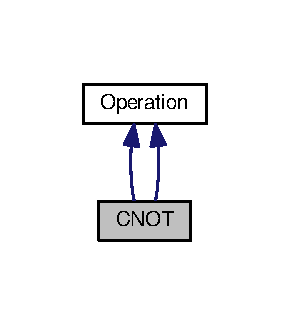
\includegraphics[width=139pt]{class_c_n_o_t__inherit__graph}
\end{center}
\end{figure}
\subsection*{Public Member Functions}
\begin{DoxyCompactItemize}
\item 
\hyperlink{class_c_n_o_t}{C\+N\+OT} $\ast$ \hyperlink{class_c_n_o_t_adaf82830347d53a38f83cc7d993f923f}{clone} ()
\begin{DoxyCompactList}\small\item\em Call to create a clone of the present class. \end{DoxyCompactList}\item 
\hyperlink{class_c_n_o_t}{C\+N\+OT} $\ast$ \hyperlink{class_c_n_o_t_ae5677074931b985f239441a96697d300}{clone} ()
\begin{DoxyCompactList}\small\item\em Call to create a clone of the present class. \end{DoxyCompactList}\item 
\hyperlink{class_c_n_o_t_a9e46511d49d6dc36e04bbd945d3483e4}{C\+N\+OT} (int qbit\+\_\+num\+\_\+in, int target\+\_\+qbit\+\_\+in, int control\+\_\+qbit\+\_\+in)
\begin{DoxyCompactList}\small\item\em Constructor of the class. \end{DoxyCompactList}\item 
\hyperlink{class_c_n_o_t_a9e46511d49d6dc36e04bbd945d3483e4}{C\+N\+OT} (int qbit\+\_\+num\+\_\+in, int target\+\_\+qbit\+\_\+in, int control\+\_\+qbit\+\_\+in)
\begin{DoxyCompactList}\small\item\em Constructor of the class. \end{DoxyCompactList}\item 
\hyperlink{struct_q_g_d___complex16}{Q\+G\+D\+\_\+\+Complex16} $\ast$ \hyperlink{class_c_n_o_t_ab664b7c42e2bd92b818bb2e4aa1aaa4b}{composite\+\_\+cnot} ()
\begin{DoxyCompactList}\small\item\em Calculate the matrix of a \hyperlink{class_c_n_o_t}{C\+N\+OT} gate operation acting on the space of qbit\+\_\+num qubits. \end{DoxyCompactList}\item 
\hyperlink{struct_q_g_d___complex16}{Q\+G\+D\+\_\+\+Complex16} $\ast$ \hyperlink{class_c_n_o_t_ad5caf96890e39fb6b7a8c7524fe324b4}{composite\+\_\+cnot} ()
\begin{DoxyCompactList}\small\item\em Calculate the matrix of a \hyperlink{class_c_n_o_t}{C\+N\+OT} gate operation acting on the space of qbit\+\_\+num qubits. \end{DoxyCompactList}\item 
int \hyperlink{class_c_n_o_t_aa74f9591e9746edde94c491a3f425315}{composite\+\_\+cnot} (\hyperlink{struct_q_g_d___complex16}{Q\+G\+D\+\_\+\+Complex16} $\ast$C\+N\+O\+T\+\_\+mtx)
\begin{DoxyCompactList}\small\item\em Calculate the matrix of a \hyperlink{class_c_n_o_t}{C\+N\+OT} gate operation acting on the space of qbit\+\_\+num qubits. \end{DoxyCompactList}\item 
int \hyperlink{class_c_n_o_t_aa74f9591e9746edde94c491a3f425315}{composite\+\_\+cnot} (\hyperlink{struct_q_g_d___complex16}{Q\+G\+D\+\_\+\+Complex16} $\ast$C\+N\+O\+T\+\_\+mtx)
\begin{DoxyCompactList}\small\item\em Calculate the matrix of a \hyperlink{class_c_n_o_t}{C\+N\+OT} gate operation acting on the space of qbit\+\_\+num qubits. \end{DoxyCompactList}\item 
int \hyperlink{class_operation_a2e9b60d334a0e0c99dede014ac989d0a}{get\+\_\+control\+\_\+qbit} ()
\begin{DoxyCompactList}\small\item\em Call to get the index of the control qubit. \end{DoxyCompactList}\item 
int \hyperlink{class_operation_a2e9b60d334a0e0c99dede014ac989d0a}{get\+\_\+control\+\_\+qbit} ()
\begin{DoxyCompactList}\small\item\em Call to get the index of the control qubit. \end{DoxyCompactList}\item 
int \hyperlink{class_operation_a670c1149cd1c675cf67bbcd861817223}{get\+\_\+parameter\+\_\+num} ()
\begin{DoxyCompactList}\small\item\em Call to get the number of free parameters. \end{DoxyCompactList}\item 
int \hyperlink{class_operation_a670c1149cd1c675cf67bbcd861817223}{get\+\_\+parameter\+\_\+num} ()
\begin{DoxyCompactList}\small\item\em Call to get the number of free parameters. \end{DoxyCompactList}\item 
int \hyperlink{class_operation_a55eee2ad4b90be085b1ec2ce018502f8}{get\+\_\+target\+\_\+qbit} ()
\begin{DoxyCompactList}\small\item\em Call to get the index of the target qubit. \end{DoxyCompactList}\item 
int \hyperlink{class_operation_a55eee2ad4b90be085b1ec2ce018502f8}{get\+\_\+target\+\_\+qbit} ()
\begin{DoxyCompactList}\small\item\em Call to get the index of the target qubit. \end{DoxyCompactList}\item 
\hyperlink{operations_2include_2_operation_8h_ad99e62941c8e4b13e5fc45ecaaf65eff}{operation\+\_\+type} \hyperlink{class_operation_acc601a7a00616fd6e2a61f61e084afac}{get\+\_\+type} ()
\begin{DoxyCompactList}\small\item\em Call to get the type of the operation. \end{DoxyCompactList}\item 
\hyperlink{operations_2include_2_operation_8h_ad99e62941c8e4b13e5fc45ecaaf65eff}{operation\+\_\+type} \hyperlink{class_operation_acc601a7a00616fd6e2a61f61e084afac}{get\+\_\+type} ()
\begin{DoxyCompactList}\small\item\em Call to get the type of the operation. \end{DoxyCompactList}\item 
\hyperlink{struct_q_g_d___complex16}{Q\+G\+D\+\_\+\+Complex16} $\ast$ \hyperlink{class_c_n_o_t_a50fefe3d884b9d5fcc20d6855e75e602}{matrix} ()
\begin{DoxyCompactList}\small\item\em Call to retrieve the operation matrix. \end{DoxyCompactList}\item 
\hyperlink{struct_q_g_d___complex16}{Q\+G\+D\+\_\+\+Complex16} $\ast$ \hyperlink{class_c_n_o_t_ae84e8aa35cc1354c896ce8c93918e7e4}{matrix} ()
\begin{DoxyCompactList}\small\item\em Call to retrieve the operation matrix. \end{DoxyCompactList}\item 
int \hyperlink{class_c_n_o_t_a8c9e4d814e5e883e0e10eb0a1e1dafe3}{matrix} (\hyperlink{struct_q_g_d___complex16}{Q\+G\+D\+\_\+\+Complex16} $\ast$retrieve\+\_\+matrix)
\begin{DoxyCompactList}\small\item\em Call to retrieve the operation matrix. \end{DoxyCompactList}\item 
int \hyperlink{class_c_n_o_t_a8c9e4d814e5e883e0e10eb0a1e1dafe3}{matrix} (\hyperlink{struct_q_g_d___complex16}{Q\+G\+D\+\_\+\+Complex16} $\ast$retrieve\+\_\+matrix)
\begin{DoxyCompactList}\small\item\em Call to retrieve the operation matrix. \end{DoxyCompactList}\item 
void \hyperlink{class_c_n_o_t_a2685ba9fe5fa414609a8ea6a9c2d18c7}{reorder\+\_\+qubits} (vector$<$ int $>$ qbit\+\_\+list)
\begin{DoxyCompactList}\small\item\em Call to reorder the qubits in the matrix of the operation. \end{DoxyCompactList}\item 
void \hyperlink{class_c_n_o_t_a2685ba9fe5fa414609a8ea6a9c2d18c7}{reorder\+\_\+qubits} (vector$<$ int $>$ qbit\+\_\+list)
\begin{DoxyCompactList}\small\item\em Call to reorder the qubits in the matrix of the operation. \end{DoxyCompactList}\item 
void \hyperlink{class_operation_a026d3dcf0ad00af99c7a9097d3cf1c74}{set\+\_\+matrix} (\hyperlink{struct_q_g_d___complex16}{Q\+G\+D\+\_\+\+Complex16} $\ast$input)
\begin{DoxyCompactList}\small\item\em Call to set the stored matrix in the operation. \end{DoxyCompactList}\item 
void \hyperlink{class_operation_a026d3dcf0ad00af99c7a9097d3cf1c74}{set\+\_\+matrix} (\hyperlink{struct_q_g_d___complex16}{Q\+G\+D\+\_\+\+Complex16} $\ast$input)
\begin{DoxyCompactList}\small\item\em Call to set the stored matrix in the operation. \end{DoxyCompactList}\item 
void \hyperlink{class_c_n_o_t_a8272bf6e7ce6705a87d1ae9ef1e09418}{set\+\_\+qbit\+\_\+num} (int \hyperlink{class_operation_aecd5fbf1dd4ea532b2e58471ff8bad69}{qbit\+\_\+num})
\begin{DoxyCompactList}\small\item\em Call to set the number of qubits spanning the matrix of the operation. \end{DoxyCompactList}\item 
void \hyperlink{class_c_n_o_t_a8272bf6e7ce6705a87d1ae9ef1e09418}{set\+\_\+qbit\+\_\+num} (int \hyperlink{class_operation_aecd5fbf1dd4ea532b2e58471ff8bad69}{qbit\+\_\+num})
\begin{DoxyCompactList}\small\item\em Call to set the number of qubits spanning the matrix of the operation. \end{DoxyCompactList}\item 
\hyperlink{class_c_n_o_t_a9074d4194dff57830d2495c245322b5b}{$\sim$\+C\+N\+OT} ()
\begin{DoxyCompactList}\small\item\em Destructor of the class. \end{DoxyCompactList}\item 
\hyperlink{class_c_n_o_t_a9074d4194dff57830d2495c245322b5b}{$\sim$\+C\+N\+OT} ()
\begin{DoxyCompactList}\small\item\em Destructor of the class. \end{DoxyCompactList}\end{DoxyCompactItemize}
\subsection*{Protected Attributes}
\begin{DoxyCompactItemize}
\item 
int \hyperlink{class_operation_a9a798ea8adec5a45fd2ca07996da88e1}{control\+\_\+qbit}
\begin{DoxyCompactList}\small\item\em The index of the qubit which acts as a control qubit (control\+\_\+qbit $>$= 0) in controlled operations. \end{DoxyCompactList}\item 
\hyperlink{struct_q_g_d___complex16}{Q\+G\+D\+\_\+\+Complex16} $\ast$ \hyperlink{class_operation_ade4d28d271ca13950d04363aac1c382e}{matrix\+\_\+alloc}
\begin{DoxyCompactList}\small\item\em Pointer to the operatrion matrix (if it is a constant general matrix) \end{DoxyCompactList}\item 
int \hyperlink{class_operation_a8236c07112cb165a00d3869363808624}{matrix\+\_\+size}
\begin{DoxyCompactList}\small\item\em The size N of the NxN matrix associated with the operations. \end{DoxyCompactList}\item 
int \hyperlink{class_operation_aa57505afe5b5ec27f6d053044b86e043}{parameter\+\_\+num}
\begin{DoxyCompactList}\small\item\em the number of free parameters of the operation \end{DoxyCompactList}\item 
int \hyperlink{class_operation_aecd5fbf1dd4ea532b2e58471ff8bad69}{qbit\+\_\+num}
\begin{DoxyCompactList}\small\item\em number of qubits spanning the matrix of the operation \end{DoxyCompactList}\item 
int \hyperlink{class_operation_a3e489b72c124b494777c71b1646bb1e9}{target\+\_\+qbit}
\begin{DoxyCompactList}\small\item\em The index of the qubit on which the operation acts (target\+\_\+qbit $>$= 0) \end{DoxyCompactList}\item 
\hyperlink{operations_2include_2_operation_8h_ad99e62941c8e4b13e5fc45ecaaf65eff}{operation\+\_\+type} \hyperlink{class_operation_ad47c56c86d62a4c775571e1600416479}{type}
\begin{DoxyCompactList}\small\item\em The type of the operation (see enumeration operation\+\_\+type) \end{DoxyCompactList}\end{DoxyCompactItemize}


\subsection{Detailed Description}
A class representing a \hyperlink{class_c_n_o_t}{C\+N\+OT} operation. 

Definition at line 35 of file operations/include/\+C\+N\+O\+T.\+h.



\subsection{Constructor \& Destructor Documentation}
\index{C\+N\+OT@{C\+N\+OT}!C\+N\+OT@{C\+N\+OT}}
\index{C\+N\+OT@{C\+N\+OT}!C\+N\+OT@{C\+N\+OT}}
\subsubsection[{\texorpdfstring{C\+N\+O\+T(int qbit\+\_\+num\+\_\+in, int target\+\_\+qbit\+\_\+in, int control\+\_\+qbit\+\_\+in)}{CNOT(int qbit_num_in, int target_qbit_in, int control_qbit_in)}}]{\setlength{\rightskip}{0pt plus 5cm}C\+N\+O\+T\+::\+C\+N\+OT (
\begin{DoxyParamCaption}
\item[{int}]{qbit\+\_\+num\+\_\+in, }
\item[{int}]{target\+\_\+qbit\+\_\+in, }
\item[{int}]{control\+\_\+qbit\+\_\+in}
\end{DoxyParamCaption}
)}\hypertarget{class_c_n_o_t_a9e46511d49d6dc36e04bbd945d3483e4}{}\label{class_c_n_o_t_a9e46511d49d6dc36e04bbd945d3483e4}


Constructor of the class. 


\begin{DoxyParams}{Parameters}
{\em qbit\+\_\+num\+\_\+in} & The number of qubits in the unitaries \\
\hline
{\em target\+\_\+qbit\+\_\+in} & The identification number of the target qubit. (0 $<$= target\+\_\+qbit $<$= qbit\+\_\+num-\/1) \\
\hline
{\em control\+\_\+qbit\+\_\+in} & The identification number of the control qubit. (0 $<$= target\+\_\+qbit $<$= qbit\+\_\+num-\/1) \\
\hline
\end{DoxyParams}


Definition at line 35 of file C\+N\+O\+T.\+cpp.



Here is the call graph for this function\+:
\nopagebreak
\begin{figure}[H]
\begin{center}
\leavevmode
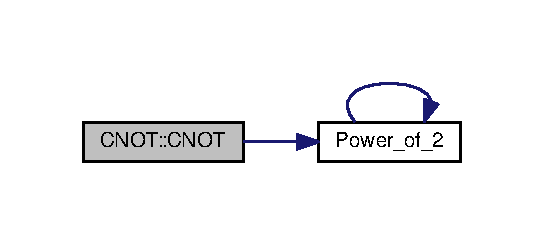
\includegraphics[width=261pt]{class_c_n_o_t_a9e46511d49d6dc36e04bbd945d3483e4_cgraph}
\end{center}
\end{figure}


\index{C\+N\+OT@{C\+N\+OT}!````~C\+N\+OT@{$\sim$\+C\+N\+OT}}
\index{````~C\+N\+OT@{$\sim$\+C\+N\+OT}!C\+N\+OT@{C\+N\+OT}}
\subsubsection[{\texorpdfstring{$\sim$\+C\+N\+O\+T()}{~CNOT()}}]{\setlength{\rightskip}{0pt plus 5cm}C\+N\+O\+T\+::$\sim$\+C\+N\+OT (
\begin{DoxyParamCaption}
{}
\end{DoxyParamCaption}
)}\hypertarget{class_c_n_o_t_a9074d4194dff57830d2495c245322b5b}{}\label{class_c_n_o_t_a9074d4194dff57830d2495c245322b5b}


Destructor of the class. 



Definition at line 69 of file C\+N\+O\+T.\+cpp.

\index{C\+N\+OT@{C\+N\+OT}!C\+N\+OT@{C\+N\+OT}}
\index{C\+N\+OT@{C\+N\+OT}!C\+N\+OT@{C\+N\+OT}}
\subsubsection[{\texorpdfstring{C\+N\+O\+T(int qbit\+\_\+num\+\_\+in, int target\+\_\+qbit\+\_\+in, int control\+\_\+qbit\+\_\+in)}{CNOT(int qbit_num_in, int target_qbit_in, int control_qbit_in)}}]{\setlength{\rightskip}{0pt plus 5cm}C\+N\+O\+T\+::\+C\+N\+OT (
\begin{DoxyParamCaption}
\item[{int}]{qbit\+\_\+num\+\_\+in, }
\item[{int}]{target\+\_\+qbit\+\_\+in, }
\item[{int}]{control\+\_\+qbit\+\_\+in}
\end{DoxyParamCaption}
)}\hypertarget{class_c_n_o_t_a9e46511d49d6dc36e04bbd945d3483e4}{}\label{class_c_n_o_t_a9e46511d49d6dc36e04bbd945d3483e4}


Constructor of the class. 


\begin{DoxyParams}{Parameters}
{\em qbit\+\_\+num\+\_\+in} & The number of qubits in the unitaries \\
\hline
{\em target\+\_\+qbit\+\_\+in} & The identification number of the target qubit. (0 $<$= target\+\_\+qbit $<$= qbit\+\_\+num-\/1) \\
\hline
{\em control\+\_\+qbit\+\_\+in} & The identification number of the control qubit. (0 $<$= target\+\_\+qbit $<$= qbit\+\_\+num-\/1) \\
\hline
\end{DoxyParams}
\index{C\+N\+OT@{C\+N\+OT}!````~C\+N\+OT@{$\sim$\+C\+N\+OT}}
\index{````~C\+N\+OT@{$\sim$\+C\+N\+OT}!C\+N\+OT@{C\+N\+OT}}
\subsubsection[{\texorpdfstring{$\sim$\+C\+N\+O\+T()}{~CNOT()}}]{\setlength{\rightskip}{0pt plus 5cm}C\+N\+O\+T\+::$\sim$\+C\+N\+OT (
\begin{DoxyParamCaption}
{}
\end{DoxyParamCaption}
)}\hypertarget{class_c_n_o_t_a9074d4194dff57830d2495c245322b5b}{}\label{class_c_n_o_t_a9074d4194dff57830d2495c245322b5b}


Destructor of the class. 



\subsection{Member Function Documentation}
\index{C\+N\+OT@{C\+N\+OT}!clone@{clone}}
\index{clone@{clone}!C\+N\+OT@{C\+N\+OT}}
\subsubsection[{\texorpdfstring{clone()}{clone()}}]{\setlength{\rightskip}{0pt plus 5cm}{\bf C\+N\+OT} $\ast$ C\+N\+O\+T\+::clone (
\begin{DoxyParamCaption}
{}
\end{DoxyParamCaption}
)}\hypertarget{class_c_n_o_t_adaf82830347d53a38f83cc7d993f923f}{}\label{class_c_n_o_t_adaf82830347d53a38f83cc7d993f923f}


Call to create a clone of the present class. 

\begin{DoxyReturn}{Returns}
Return with a pointer pointing to the cloned object 
\end{DoxyReturn}


Definition at line 219 of file C\+N\+O\+T.\+cpp.



Here is the call graph for this function\+:
\nopagebreak
\begin{figure}[H]
\begin{center}
\leavevmode
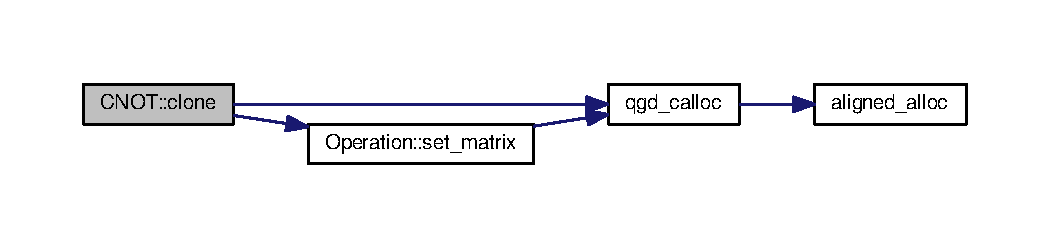
\includegraphics[width=350pt]{class_c_n_o_t_adaf82830347d53a38f83cc7d993f923f_cgraph}
\end{center}
\end{figure}




Here is the caller graph for this function\+:
\nopagebreak
\begin{figure}[H]
\begin{center}
\leavevmode
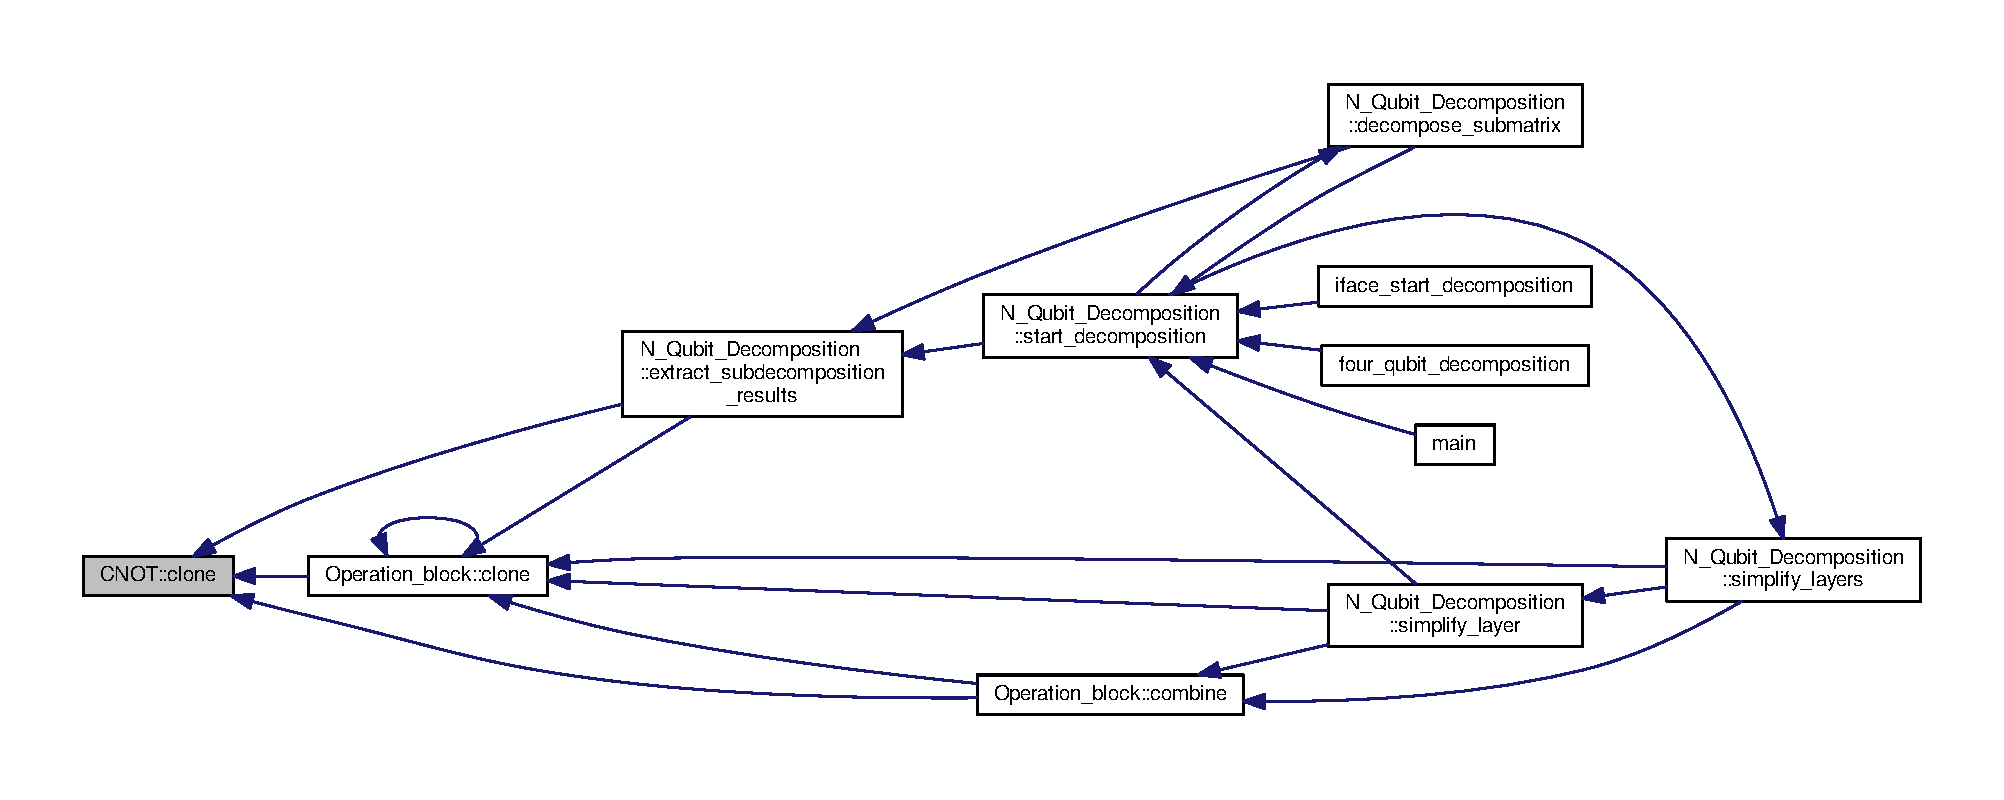
\includegraphics[width=350pt]{class_c_n_o_t_adaf82830347d53a38f83cc7d993f923f_icgraph}
\end{center}
\end{figure}


\index{C\+N\+OT@{C\+N\+OT}!clone@{clone}}
\index{clone@{clone}!C\+N\+OT@{C\+N\+OT}}
\subsubsection[{\texorpdfstring{clone()}{clone()}}]{\setlength{\rightskip}{0pt plus 5cm}{\bf C\+N\+OT}$\ast$ C\+N\+O\+T\+::clone (
\begin{DoxyParamCaption}
{}
\end{DoxyParamCaption}
)}\hypertarget{class_c_n_o_t_ae5677074931b985f239441a96697d300}{}\label{class_c_n_o_t_ae5677074931b985f239441a96697d300}


Call to create a clone of the present class. 

\begin{DoxyReturn}{Returns}
Return with a pointer pointing to the cloned object 
\end{DoxyReturn}
\index{C\+N\+OT@{C\+N\+OT}!composite\+\_\+cnot@{composite\+\_\+cnot}}
\index{composite\+\_\+cnot@{composite\+\_\+cnot}!C\+N\+OT@{C\+N\+OT}}
\subsubsection[{\texorpdfstring{composite\+\_\+cnot()}{composite_cnot()}}]{\setlength{\rightskip}{0pt plus 5cm}{\bf Q\+G\+D\+\_\+\+Complex16}$\ast$ C\+N\+O\+T\+::composite\+\_\+cnot (
\begin{DoxyParamCaption}
{}
\end{DoxyParamCaption}
)}\hypertarget{class_c_n_o_t_ad5caf96890e39fb6b7a8c7524fe324b4}{}\label{class_c_n_o_t_ad5caf96890e39fb6b7a8c7524fe324b4}


Calculate the matrix of a \hyperlink{class_c_n_o_t}{C\+N\+OT} gate operation acting on the space of qbit\+\_\+num qubits. 

\begin{DoxyReturn}{Returns}
Returns with a pointer to the operation matrix 
\end{DoxyReturn}
\index{C\+N\+OT@{C\+N\+OT}!composite\+\_\+cnot@{composite\+\_\+cnot}}
\index{composite\+\_\+cnot@{composite\+\_\+cnot}!C\+N\+OT@{C\+N\+OT}}
\subsubsection[{\texorpdfstring{composite\+\_\+cnot()}{composite_cnot()}}]{\setlength{\rightskip}{0pt plus 5cm}{\bf Q\+G\+D\+\_\+\+Complex16} $\ast$ C\+N\+O\+T\+::composite\+\_\+cnot (
\begin{DoxyParamCaption}
{}
\end{DoxyParamCaption}
)}\hypertarget{class_c_n_o_t_ab664b7c42e2bd92b818bb2e4aa1aaa4b}{}\label{class_c_n_o_t_ab664b7c42e2bd92b818bb2e4aa1aaa4b}


Calculate the matrix of a \hyperlink{class_c_n_o_t}{C\+N\+OT} gate operation acting on the space of qbit\+\_\+num qubits. 

\begin{DoxyReturn}{Returns}
Returns with a pointer to the operation matrix 
\end{DoxyReturn}


Definition at line 97 of file C\+N\+O\+T.\+cpp.



Here is the call graph for this function\+:
\nopagebreak
\begin{figure}[H]
\begin{center}
\leavevmode
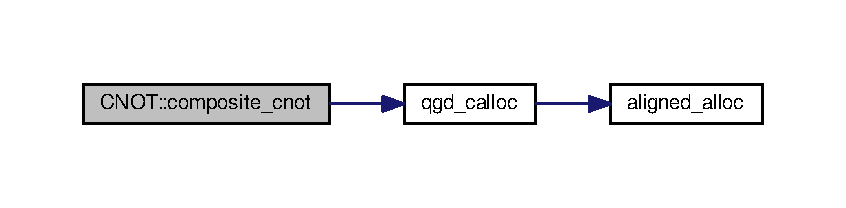
\includegraphics[width=350pt]{class_c_n_o_t_ab664b7c42e2bd92b818bb2e4aa1aaa4b_cgraph}
\end{center}
\end{figure}


\index{C\+N\+OT@{C\+N\+OT}!composite\+\_\+cnot@{composite\+\_\+cnot}}
\index{composite\+\_\+cnot@{composite\+\_\+cnot}!C\+N\+OT@{C\+N\+OT}}
\subsubsection[{\texorpdfstring{composite\+\_\+cnot(\+Q\+G\+D\+\_\+\+Complex16 $\ast$\+C\+N\+O\+T\+\_\+mtx)}{composite_cnot(QGD_Complex16 *CNOT_mtx)}}]{\setlength{\rightskip}{0pt plus 5cm}int C\+N\+O\+T\+::composite\+\_\+cnot (
\begin{DoxyParamCaption}
\item[{{\bf Q\+G\+D\+\_\+\+Complex16} $\ast$}]{C\+N\+O\+T\+\_\+mtx}
\end{DoxyParamCaption}
)}\hypertarget{class_c_n_o_t_aa74f9591e9746edde94c491a3f425315}{}\label{class_c_n_o_t_aa74f9591e9746edde94c491a3f425315}


Calculate the matrix of a \hyperlink{class_c_n_o_t}{C\+N\+OT} gate operation acting on the space of qbit\+\_\+num qubits. 


\begin{DoxyParams}{Parameters}
{\em C\+N\+O\+T\+\_\+mtx} & A pointer to the preallocated array of the operation matrix. \\
\hline
\end{DoxyParams}
\begin{DoxyReturn}{Returns}
Returns with 0 on success. 
\end{DoxyReturn}


Definition at line 114 of file C\+N\+O\+T.\+cpp.



Here is the call graph for this function\+:
\nopagebreak
\begin{figure}[H]
\begin{center}
\leavevmode
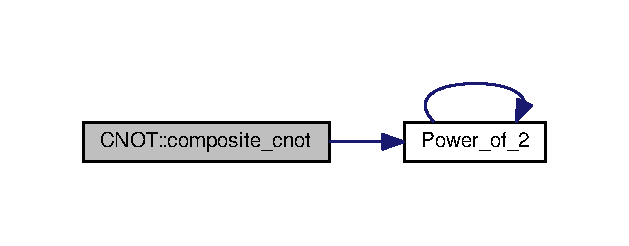
\includegraphics[width=302pt]{class_c_n_o_t_aa74f9591e9746edde94c491a3f425315_cgraph}
\end{center}
\end{figure}


\index{C\+N\+OT@{C\+N\+OT}!composite\+\_\+cnot@{composite\+\_\+cnot}}
\index{composite\+\_\+cnot@{composite\+\_\+cnot}!C\+N\+OT@{C\+N\+OT}}
\subsubsection[{\texorpdfstring{composite\+\_\+cnot(\+Q\+G\+D\+\_\+\+Complex16 $\ast$\+C\+N\+O\+T\+\_\+mtx)}{composite_cnot(QGD_Complex16 *CNOT_mtx)}}]{\setlength{\rightskip}{0pt plus 5cm}int C\+N\+O\+T\+::composite\+\_\+cnot (
\begin{DoxyParamCaption}
\item[{{\bf Q\+G\+D\+\_\+\+Complex16} $\ast$}]{C\+N\+O\+T\+\_\+mtx}
\end{DoxyParamCaption}
)}\hypertarget{class_c_n_o_t_aa74f9591e9746edde94c491a3f425315}{}\label{class_c_n_o_t_aa74f9591e9746edde94c491a3f425315}


Calculate the matrix of a \hyperlink{class_c_n_o_t}{C\+N\+OT} gate operation acting on the space of qbit\+\_\+num qubits. 


\begin{DoxyParams}{Parameters}
{\em C\+N\+O\+T\+\_\+mtx} & A pointer to the preallocated array of the operation matrix. \\
\hline
\end{DoxyParams}
\begin{DoxyReturn}{Returns}
Returns with 0 on success. 
\end{DoxyReturn}
\index{C\+N\+OT@{C\+N\+OT}!get\+\_\+control\+\_\+qbit@{get\+\_\+control\+\_\+qbit}}
\index{get\+\_\+control\+\_\+qbit@{get\+\_\+control\+\_\+qbit}!C\+N\+OT@{C\+N\+OT}}
\subsubsection[{\texorpdfstring{get\+\_\+control\+\_\+qbit()}{get_control_qbit()}}]{\setlength{\rightskip}{0pt plus 5cm}int Operation\+::get\+\_\+control\+\_\+qbit (
\begin{DoxyParamCaption}
{}
\end{DoxyParamCaption}
)\hspace{0.3cm}{\ttfamily [inherited]}}\hypertarget{class_operation_a2e9b60d334a0e0c99dede014ac989d0a}{}\label{class_operation_a2e9b60d334a0e0c99dede014ac989d0a}


Call to get the index of the control qubit. 

\begin{DoxyReturn}{Returns}
Return with the index of the control qubit (return with -\/1 if control qubit was not set) 
\end{DoxyReturn}


Definition at line 178 of file Operation.\+cpp.



Here is the caller graph for this function\+:
\nopagebreak
\begin{figure}[H]
\begin{center}
\leavevmode
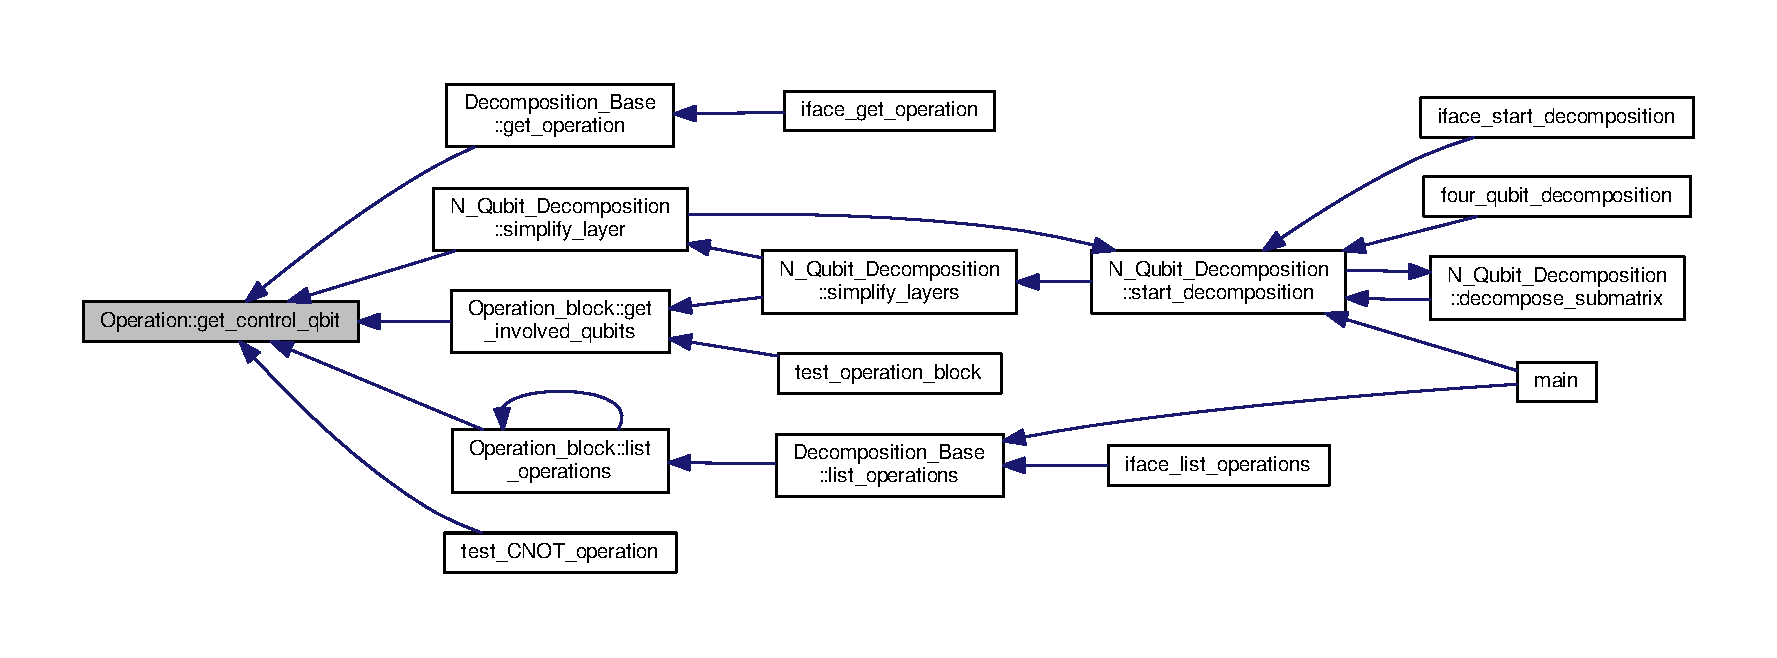
\includegraphics[width=350pt]{class_operation_a2e9b60d334a0e0c99dede014ac989d0a_icgraph}
\end{center}
\end{figure}


\index{C\+N\+OT@{C\+N\+OT}!get\+\_\+control\+\_\+qbit@{get\+\_\+control\+\_\+qbit}}
\index{get\+\_\+control\+\_\+qbit@{get\+\_\+control\+\_\+qbit}!C\+N\+OT@{C\+N\+OT}}
\subsubsection[{\texorpdfstring{get\+\_\+control\+\_\+qbit()}{get_control_qbit()}}]{\setlength{\rightskip}{0pt plus 5cm}int Operation\+::get\+\_\+control\+\_\+qbit (
\begin{DoxyParamCaption}
{}
\end{DoxyParamCaption}
)\hspace{0.3cm}{\ttfamily [inherited]}}\hypertarget{class_operation_a2e9b60d334a0e0c99dede014ac989d0a}{}\label{class_operation_a2e9b60d334a0e0c99dede014ac989d0a}


Call to get the index of the control qubit. 

\begin{DoxyReturn}{Returns}
Return with the index of the control qubit (return with -\/1 if control qubit was not set) 
\end{DoxyReturn}
\index{C\+N\+OT@{C\+N\+OT}!get\+\_\+parameter\+\_\+num@{get\+\_\+parameter\+\_\+num}}
\index{get\+\_\+parameter\+\_\+num@{get\+\_\+parameter\+\_\+num}!C\+N\+OT@{C\+N\+OT}}
\subsubsection[{\texorpdfstring{get\+\_\+parameter\+\_\+num()}{get_parameter_num()}}]{\setlength{\rightskip}{0pt plus 5cm}int Operation\+::get\+\_\+parameter\+\_\+num (
\begin{DoxyParamCaption}
{}
\end{DoxyParamCaption}
)\hspace{0.3cm}{\ttfamily [inherited]}}\hypertarget{class_operation_a670c1149cd1c675cf67bbcd861817223}{}\label{class_operation_a670c1149cd1c675cf67bbcd861817223}


Call to get the number of free parameters. 

\begin{DoxyReturn}{Returns}
Return with the number of the free parameters 
\end{DoxyReturn}


Definition at line 186 of file Operation.\+cpp.



Here is the caller graph for this function\+:
\nopagebreak
\begin{figure}[H]
\begin{center}
\leavevmode
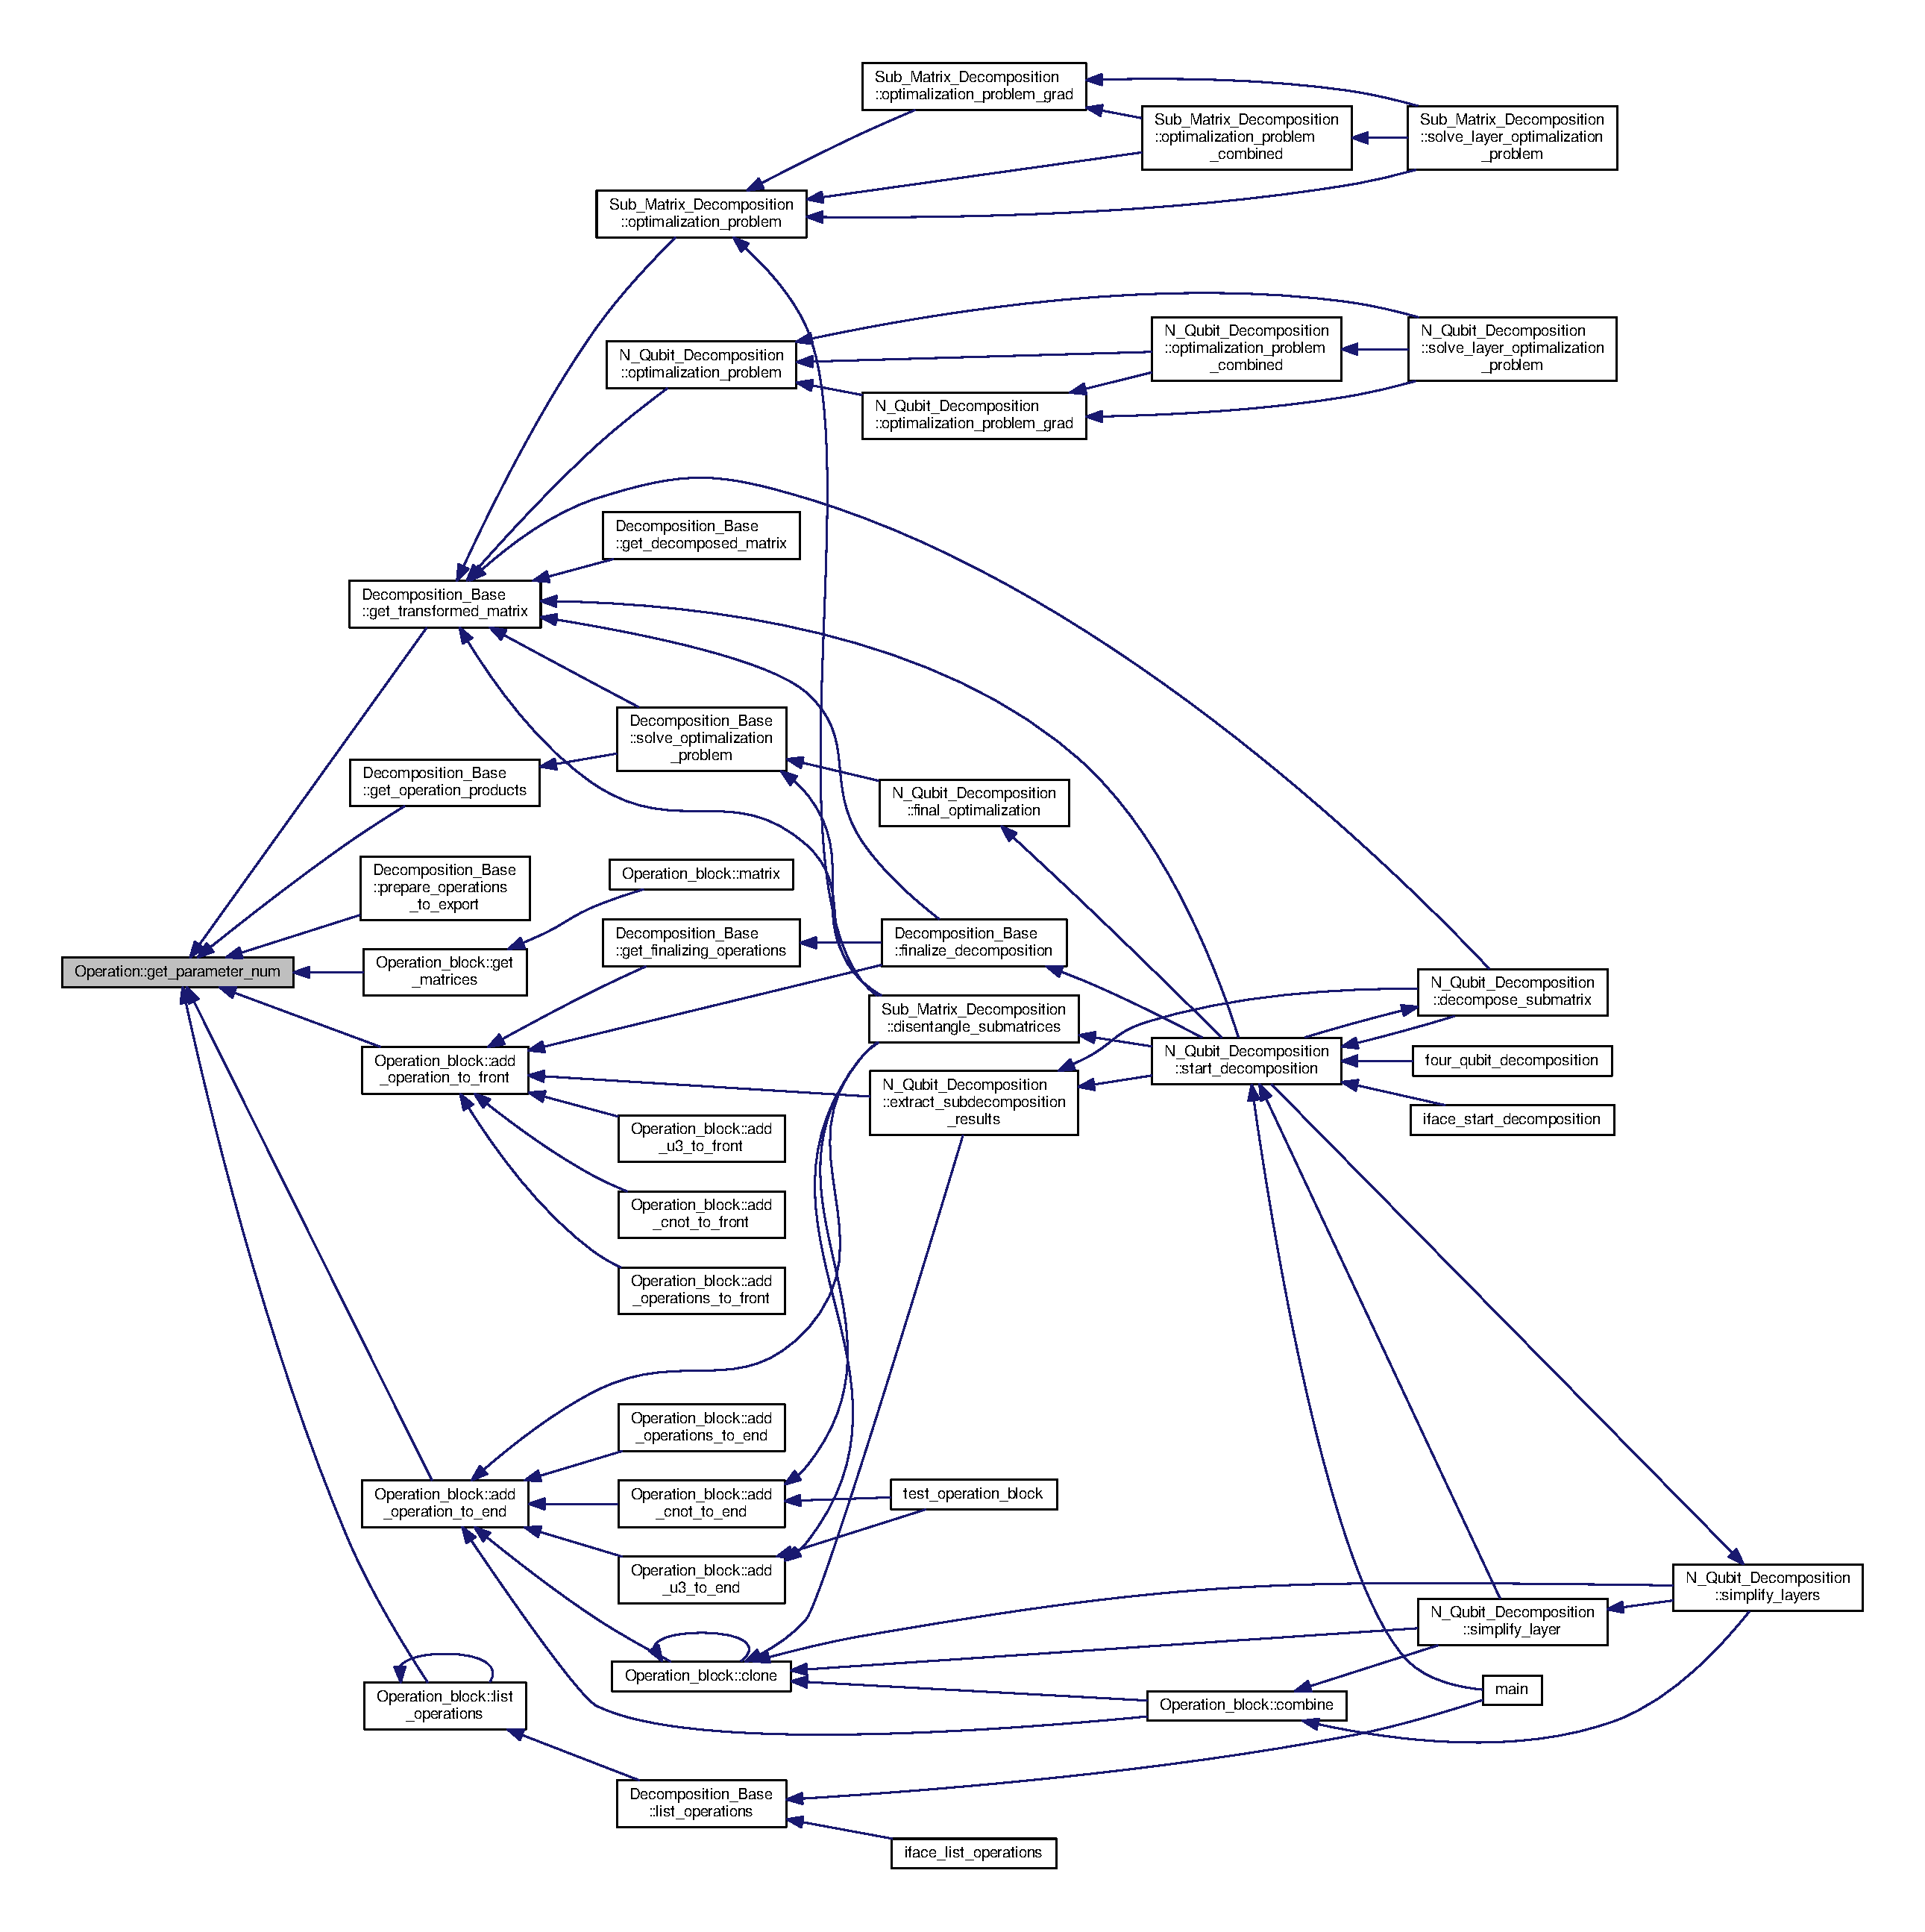
\includegraphics[width=350pt]{class_operation_a670c1149cd1c675cf67bbcd861817223_icgraph}
\end{center}
\end{figure}


\index{C\+N\+OT@{C\+N\+OT}!get\+\_\+parameter\+\_\+num@{get\+\_\+parameter\+\_\+num}}
\index{get\+\_\+parameter\+\_\+num@{get\+\_\+parameter\+\_\+num}!C\+N\+OT@{C\+N\+OT}}
\subsubsection[{\texorpdfstring{get\+\_\+parameter\+\_\+num()}{get_parameter_num()}}]{\setlength{\rightskip}{0pt plus 5cm}int Operation\+::get\+\_\+parameter\+\_\+num (
\begin{DoxyParamCaption}
{}
\end{DoxyParamCaption}
)\hspace{0.3cm}{\ttfamily [inherited]}}\hypertarget{class_operation_a670c1149cd1c675cf67bbcd861817223}{}\label{class_operation_a670c1149cd1c675cf67bbcd861817223}


Call to get the number of free parameters. 

\begin{DoxyReturn}{Returns}
Return with the number of the free parameters 
\end{DoxyReturn}
\index{C\+N\+OT@{C\+N\+OT}!get\+\_\+target\+\_\+qbit@{get\+\_\+target\+\_\+qbit}}
\index{get\+\_\+target\+\_\+qbit@{get\+\_\+target\+\_\+qbit}!C\+N\+OT@{C\+N\+OT}}
\subsubsection[{\texorpdfstring{get\+\_\+target\+\_\+qbit()}{get_target_qbit()}}]{\setlength{\rightskip}{0pt plus 5cm}int Operation\+::get\+\_\+target\+\_\+qbit (
\begin{DoxyParamCaption}
{}
\end{DoxyParamCaption}
)\hspace{0.3cm}{\ttfamily [inherited]}}\hypertarget{class_operation_a55eee2ad4b90be085b1ec2ce018502f8}{}\label{class_operation_a55eee2ad4b90be085b1ec2ce018502f8}


Call to get the index of the target qubit. 

\begin{DoxyReturn}{Returns}
Return with the index of the target qubit (return with -\/1 if target qubit was not set) 
\end{DoxyReturn}


Definition at line 170 of file Operation.\+cpp.



Here is the caller graph for this function\+:
\nopagebreak
\begin{figure}[H]
\begin{center}
\leavevmode
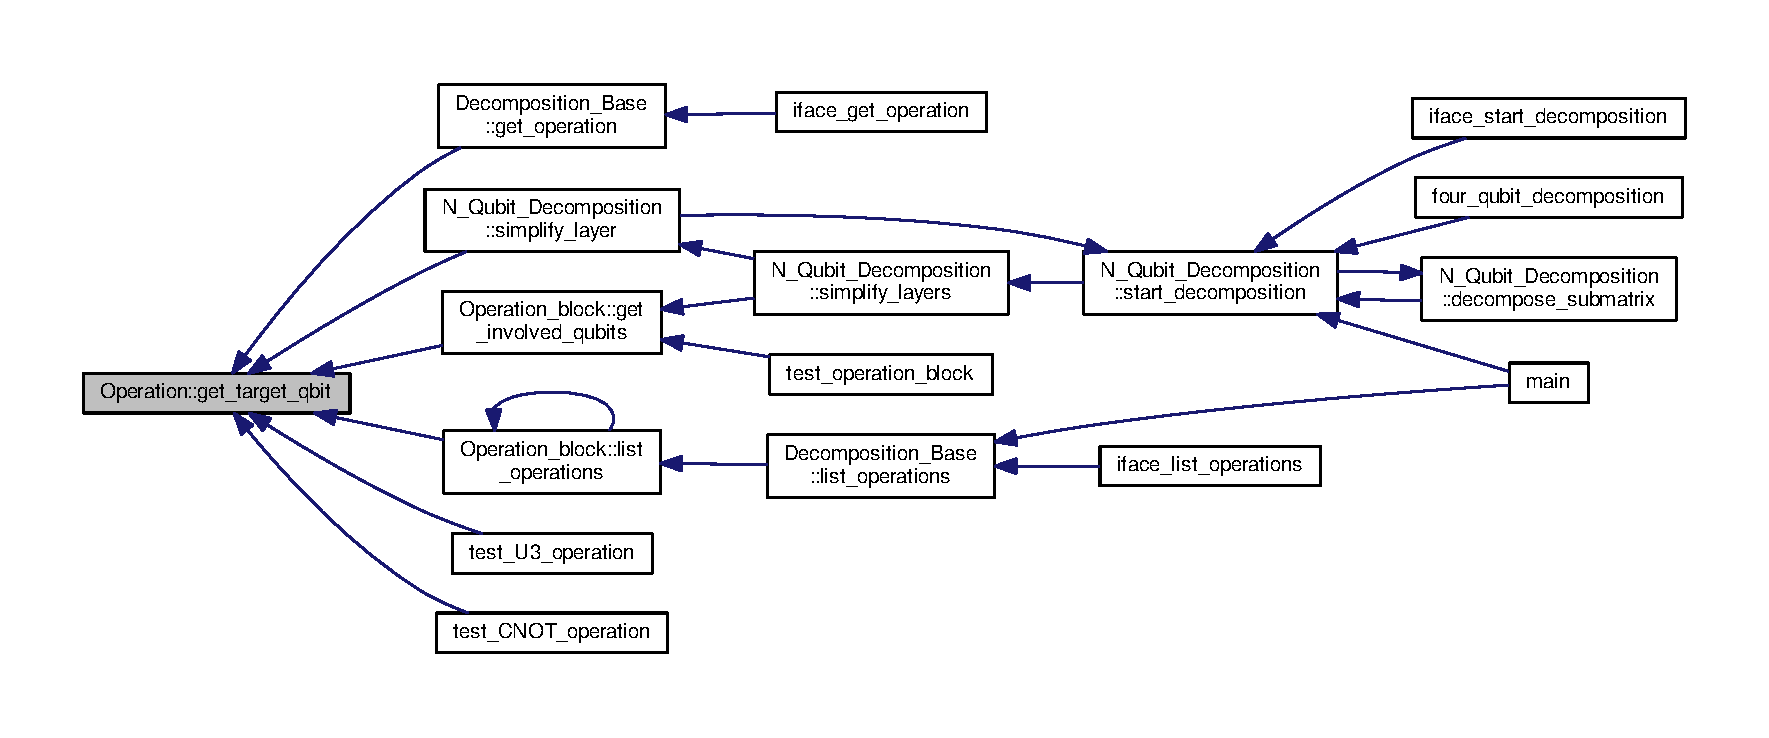
\includegraphics[width=350pt]{class_operation_a55eee2ad4b90be085b1ec2ce018502f8_icgraph}
\end{center}
\end{figure}


\index{C\+N\+OT@{C\+N\+OT}!get\+\_\+target\+\_\+qbit@{get\+\_\+target\+\_\+qbit}}
\index{get\+\_\+target\+\_\+qbit@{get\+\_\+target\+\_\+qbit}!C\+N\+OT@{C\+N\+OT}}
\subsubsection[{\texorpdfstring{get\+\_\+target\+\_\+qbit()}{get_target_qbit()}}]{\setlength{\rightskip}{0pt plus 5cm}int Operation\+::get\+\_\+target\+\_\+qbit (
\begin{DoxyParamCaption}
{}
\end{DoxyParamCaption}
)\hspace{0.3cm}{\ttfamily [inherited]}}\hypertarget{class_operation_a55eee2ad4b90be085b1ec2ce018502f8}{}\label{class_operation_a55eee2ad4b90be085b1ec2ce018502f8}


Call to get the index of the target qubit. 

\begin{DoxyReturn}{Returns}
Return with the index of the target qubit (return with -\/1 if target qubit was not set) 
\end{DoxyReturn}
\index{C\+N\+OT@{C\+N\+OT}!get\+\_\+type@{get\+\_\+type}}
\index{get\+\_\+type@{get\+\_\+type}!C\+N\+OT@{C\+N\+OT}}
\subsubsection[{\texorpdfstring{get\+\_\+type()}{get_type()}}]{\setlength{\rightskip}{0pt plus 5cm}{\bf operation\+\_\+type} Operation\+::get\+\_\+type (
\begin{DoxyParamCaption}
{}
\end{DoxyParamCaption}
)\hspace{0.3cm}{\ttfamily [inherited]}}\hypertarget{class_operation_acc601a7a00616fd6e2a61f61e084afac}{}\label{class_operation_acc601a7a00616fd6e2a61f61e084afac}


Call to get the type of the operation. 

\begin{DoxyReturn}{Returns}
Return with the type of the operation (see operation\+\_\+type for details)

Return with the type of the operation (see  for details) 
\end{DoxyReturn}


Definition at line 195 of file Operation.\+cpp.



Here is the caller graph for this function\+:
\nopagebreak
\begin{figure}[H]
\begin{center}
\leavevmode
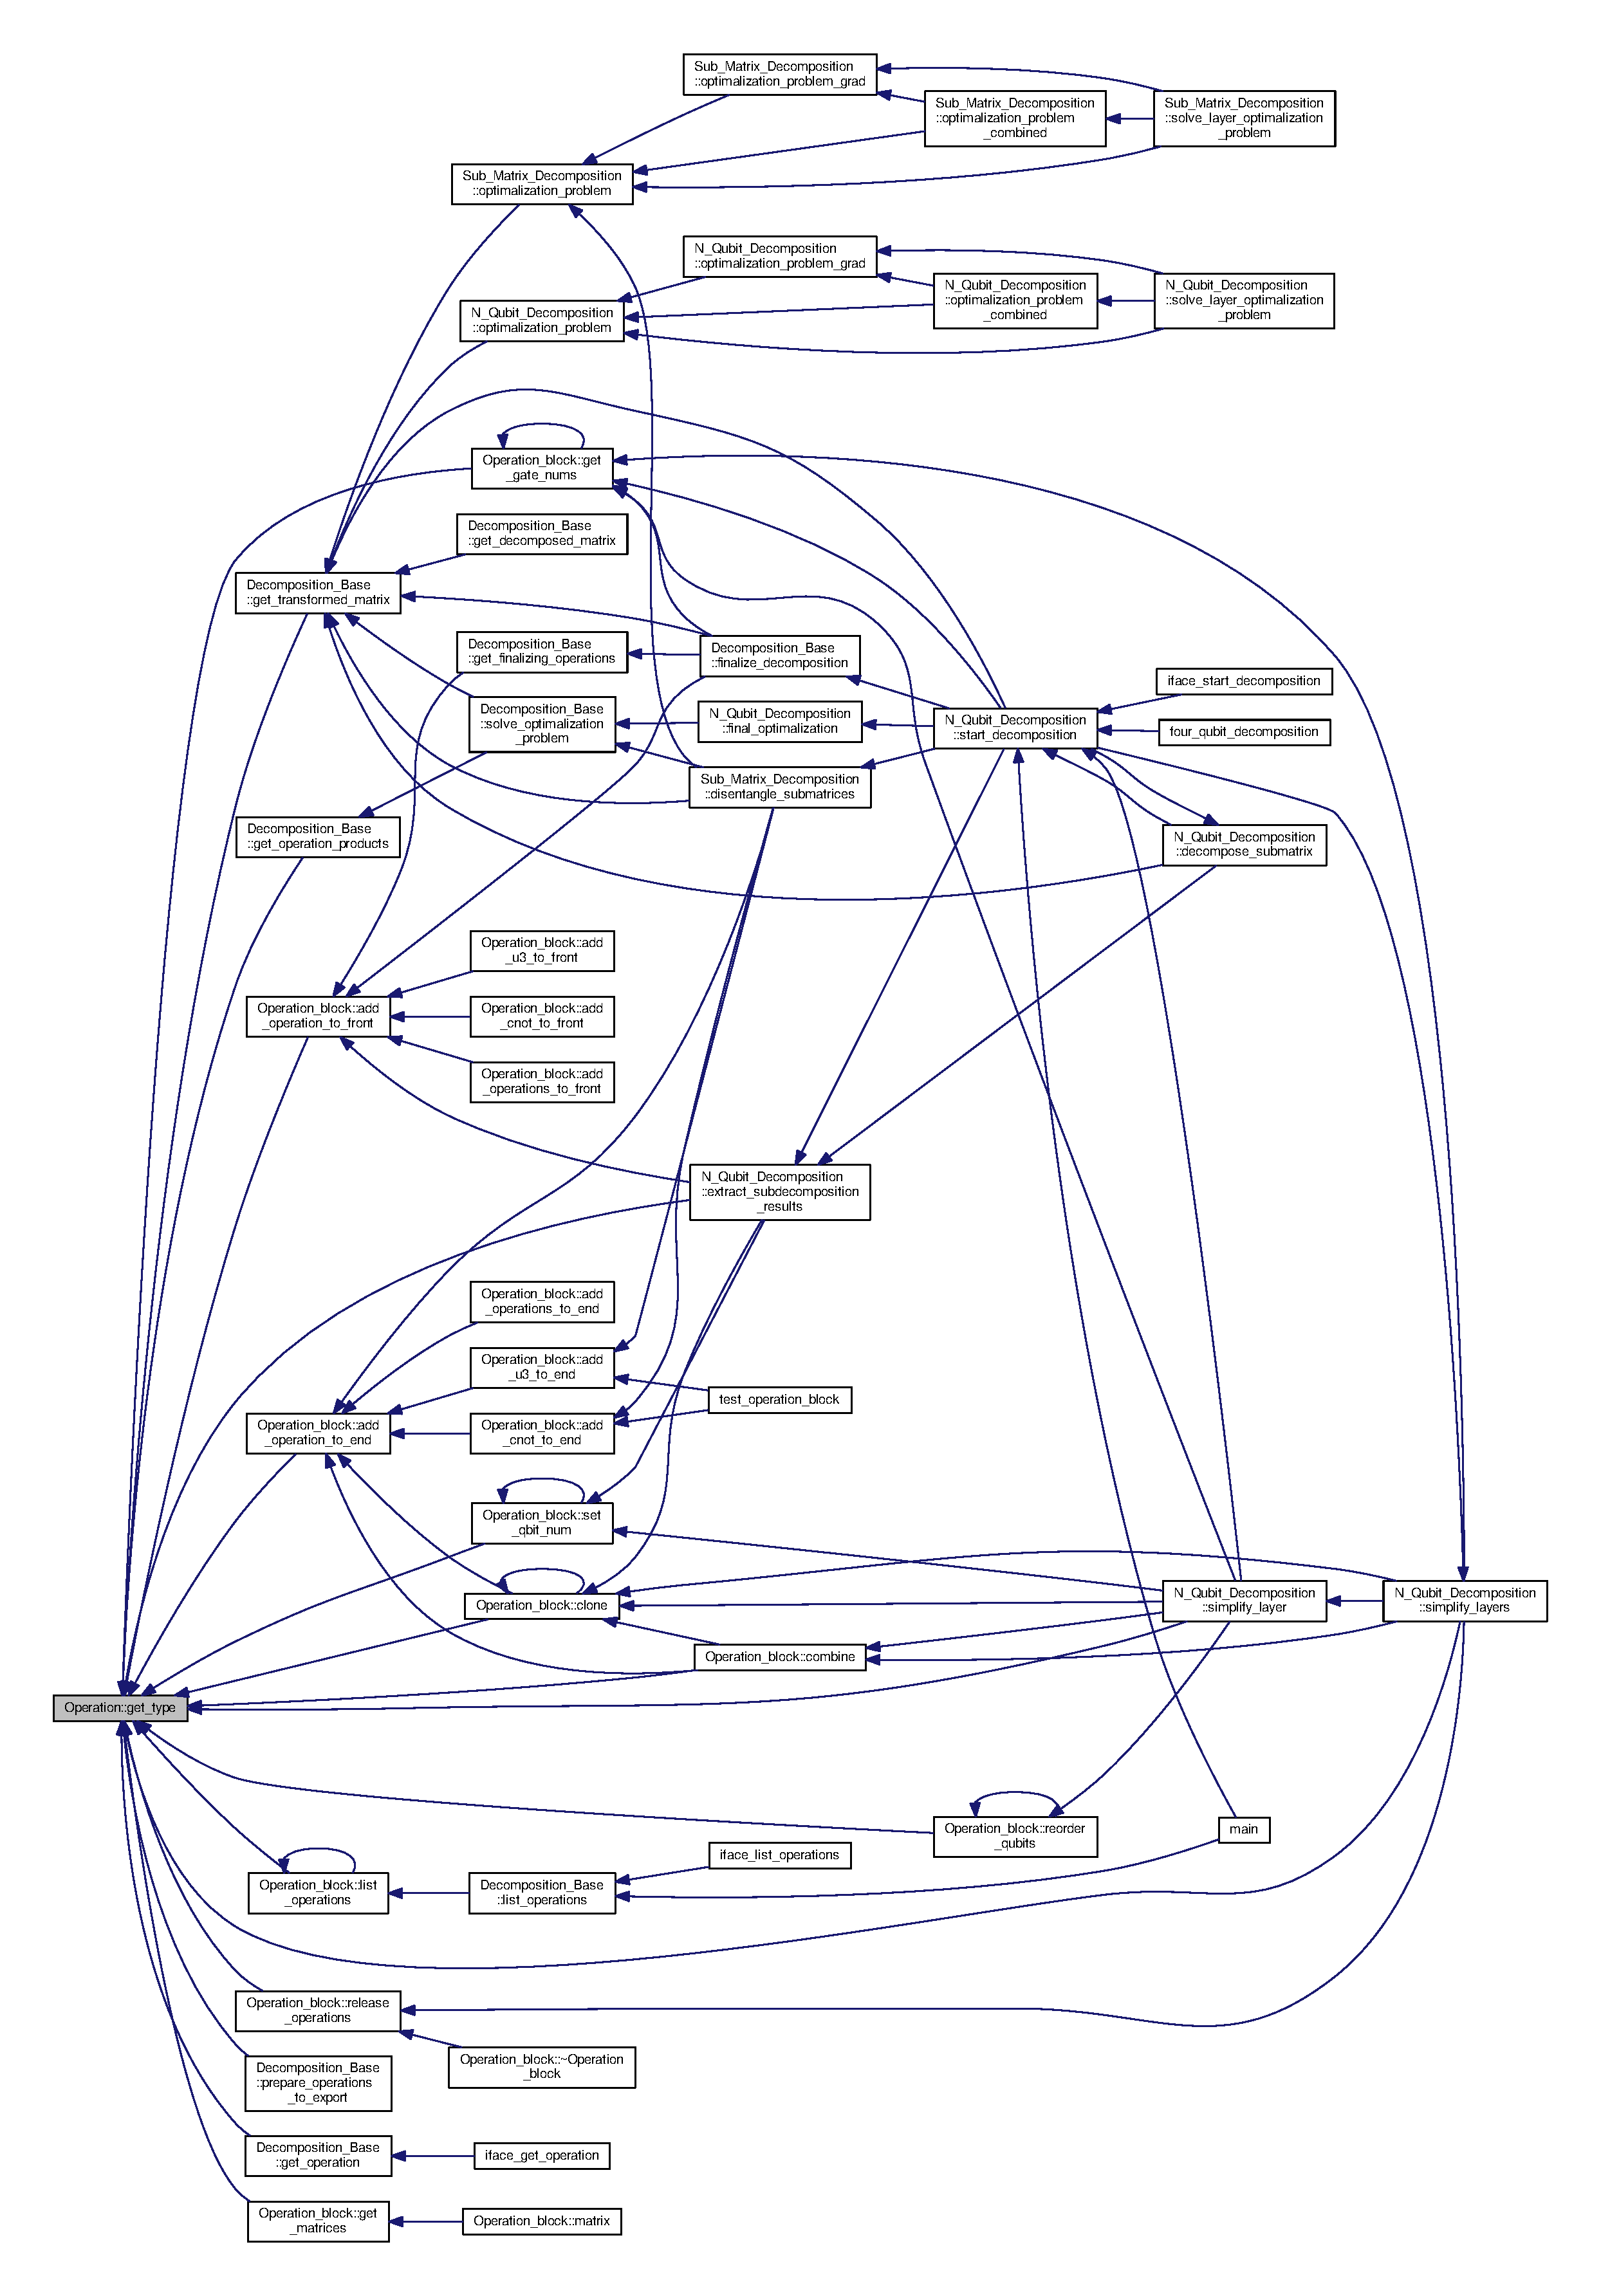
\includegraphics[width=350pt]{class_operation_acc601a7a00616fd6e2a61f61e084afac_icgraph}
\end{center}
\end{figure}


\index{C\+N\+OT@{C\+N\+OT}!get\+\_\+type@{get\+\_\+type}}
\index{get\+\_\+type@{get\+\_\+type}!C\+N\+OT@{C\+N\+OT}}
\subsubsection[{\texorpdfstring{get\+\_\+type()}{get_type()}}]{\setlength{\rightskip}{0pt plus 5cm}{\bf operation\+\_\+type} Operation\+::get\+\_\+type (
\begin{DoxyParamCaption}
{}
\end{DoxyParamCaption}
)\hspace{0.3cm}{\ttfamily [inherited]}}\hypertarget{class_operation_acc601a7a00616fd6e2a61f61e084afac}{}\label{class_operation_acc601a7a00616fd6e2a61f61e084afac}


Call to get the type of the operation. 

\begin{DoxyReturn}{Returns}
Return with the type of the operation (see operation\+\_\+type for details) 
\end{DoxyReturn}
\index{C\+N\+OT@{C\+N\+OT}!matrix@{matrix}}
\index{matrix@{matrix}!C\+N\+OT@{C\+N\+OT}}
\subsubsection[{\texorpdfstring{matrix()}{matrix()}}]{\setlength{\rightskip}{0pt plus 5cm}{\bf Q\+G\+D\+\_\+\+Complex16}$\ast$ C\+N\+O\+T\+::matrix (
\begin{DoxyParamCaption}
{}
\end{DoxyParamCaption}
)\hspace{0.3cm}{\ttfamily [virtual]}}\hypertarget{class_c_n_o_t_ae84e8aa35cc1354c896ce8c93918e7e4}{}\label{class_c_n_o_t_ae84e8aa35cc1354c896ce8c93918e7e4}


Call to retrieve the operation matrix. 

\begin{DoxyReturn}{Returns}
Returns with a pointer to the operation matrix 
\end{DoxyReturn}


Reimplemented from \hyperlink{class_operation_acf7d1765143285ff73772ae860109988}{Operation}.

\index{C\+N\+OT@{C\+N\+OT}!matrix@{matrix}}
\index{matrix@{matrix}!C\+N\+OT@{C\+N\+OT}}
\subsubsection[{\texorpdfstring{matrix()}{matrix()}}]{\setlength{\rightskip}{0pt plus 5cm}{\bf Q\+G\+D\+\_\+\+Complex16} $\ast$ C\+N\+O\+T\+::matrix (
\begin{DoxyParamCaption}
{}
\end{DoxyParamCaption}
)\hspace{0.3cm}{\ttfamily [virtual]}}\hypertarget{class_c_n_o_t_a50fefe3d884b9d5fcc20d6855e75e602}{}\label{class_c_n_o_t_a50fefe3d884b9d5fcc20d6855e75e602}


Call to retrieve the operation matrix. 

Call to terive the operation matrix.

\begin{DoxyReturn}{Returns}
Returns with a pointer to the operation matrix 
\end{DoxyReturn}


Reimplemented from \hyperlink{class_operation_acf7d1765143285ff73772ae860109988}{Operation}.



Definition at line 77 of file C\+N\+O\+T.\+cpp.



Here is the caller graph for this function\+:
\nopagebreak
\begin{figure}[H]
\begin{center}
\leavevmode
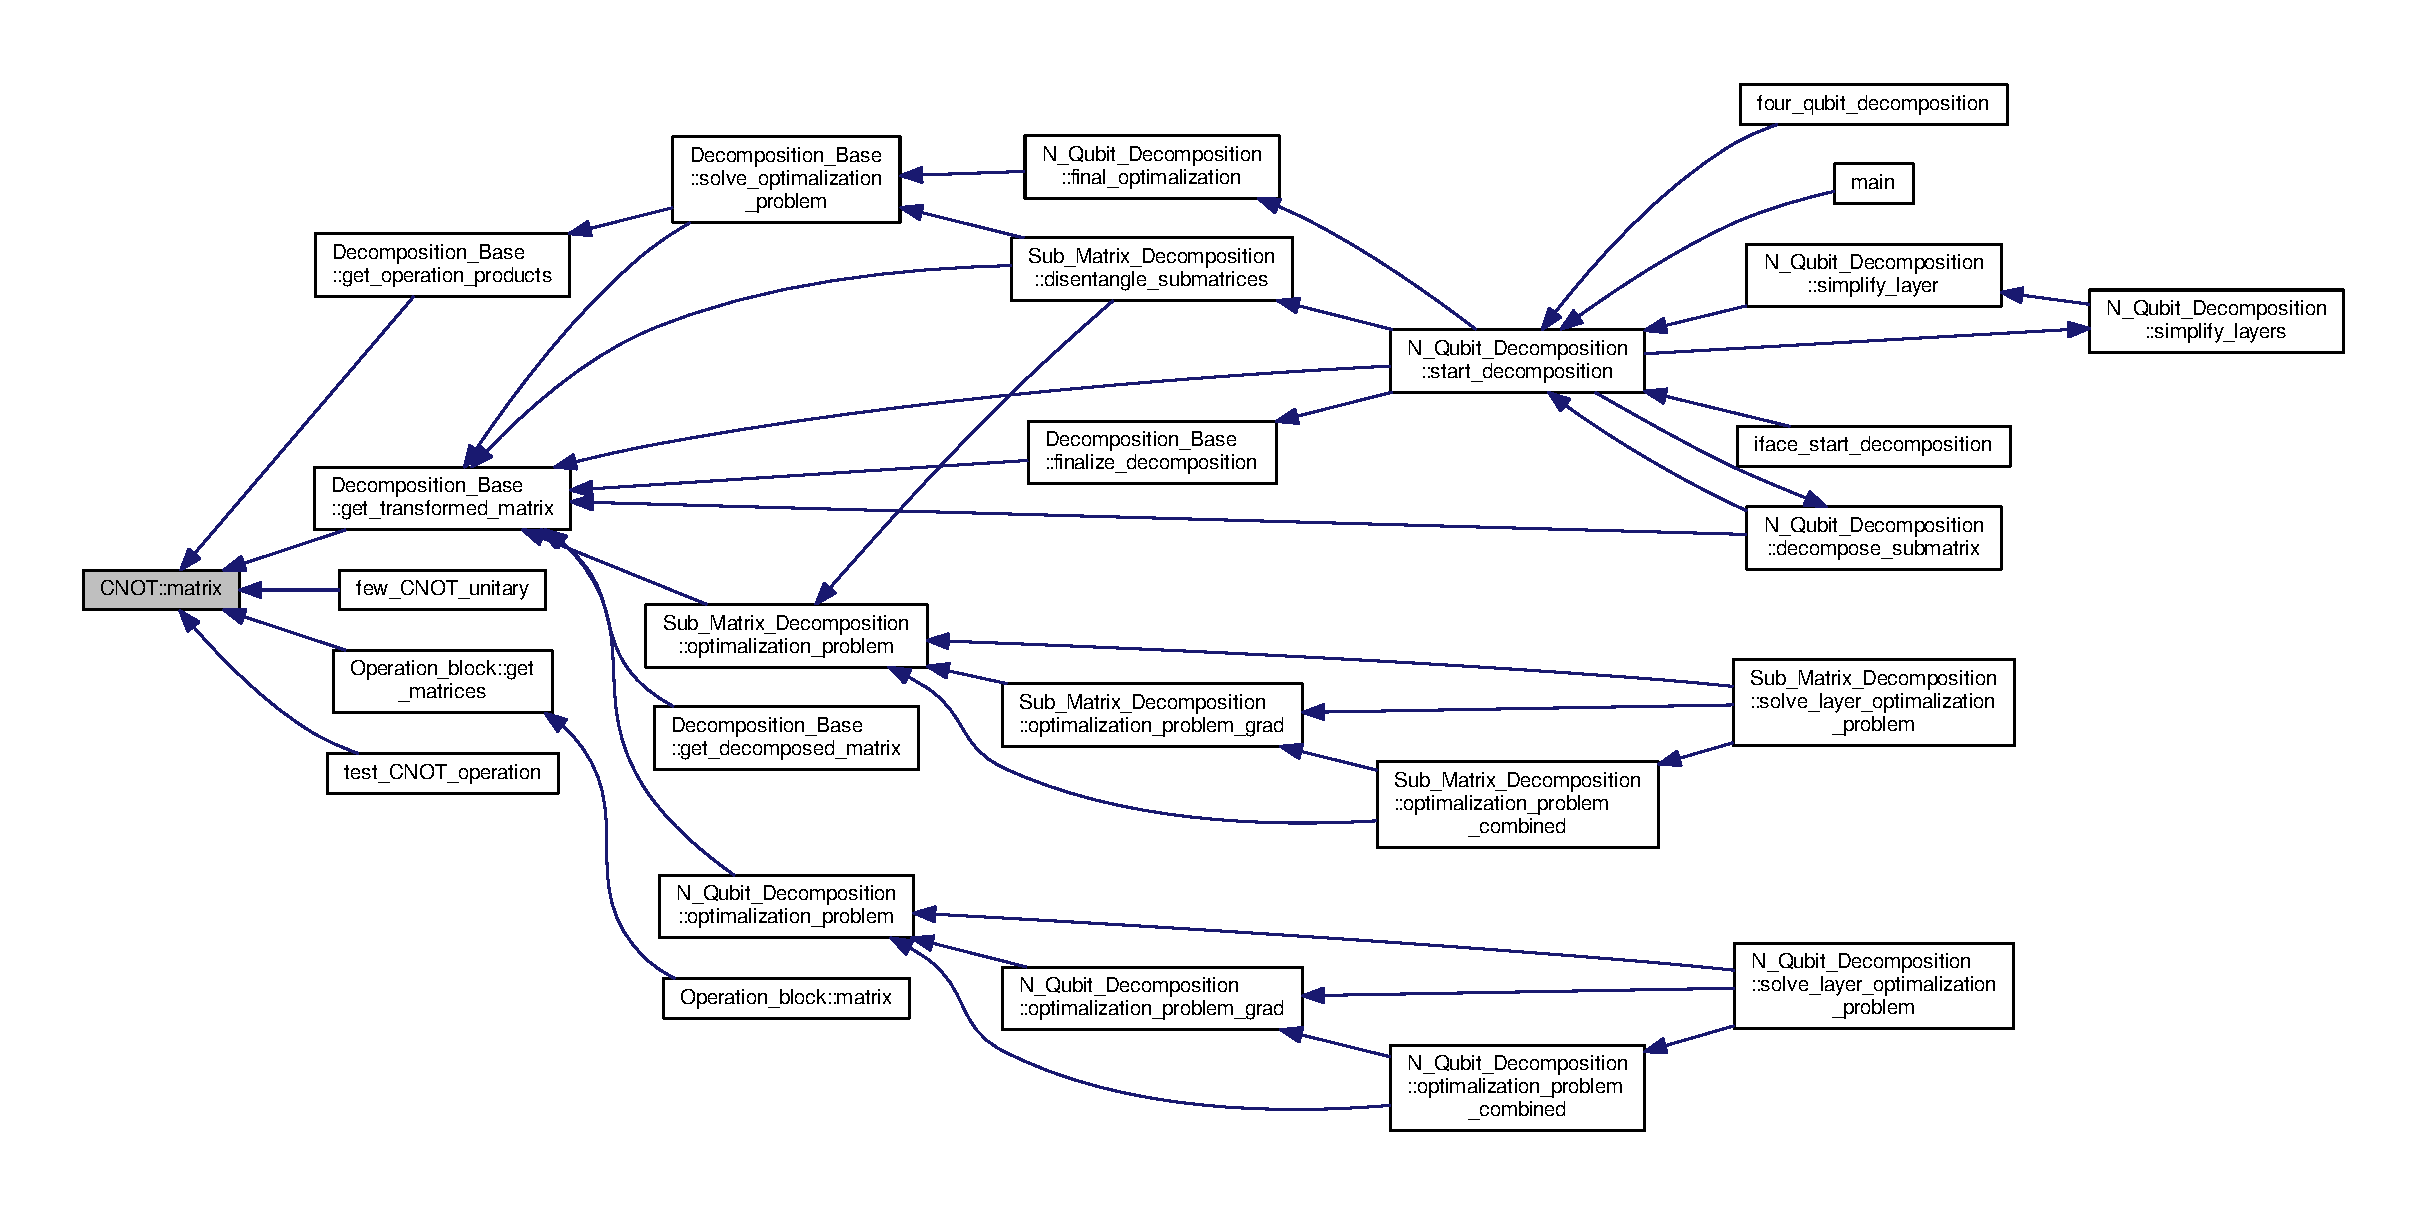
\includegraphics[width=350pt]{class_c_n_o_t_a50fefe3d884b9d5fcc20d6855e75e602_icgraph}
\end{center}
\end{figure}


\index{C\+N\+OT@{C\+N\+OT}!matrix@{matrix}}
\index{matrix@{matrix}!C\+N\+OT@{C\+N\+OT}}
\subsubsection[{\texorpdfstring{matrix(\+Q\+G\+D\+\_\+\+Complex16 $\ast$retrieve\+\_\+matrix)}{matrix(QGD_Complex16 *retrieve_matrix)}}]{\setlength{\rightskip}{0pt plus 5cm}int C\+N\+O\+T\+::matrix (
\begin{DoxyParamCaption}
\item[{{\bf Q\+G\+D\+\_\+\+Complex16} $\ast$}]{retrieve\+\_\+matrix}
\end{DoxyParamCaption}
)\hspace{0.3cm}{\ttfamily [virtual]}}\hypertarget{class_c_n_o_t_a8c9e4d814e5e883e0e10eb0a1e1dafe3}{}\label{class_c_n_o_t_a8c9e4d814e5e883e0e10eb0a1e1dafe3}


Call to retrieve the operation matrix. 


\begin{DoxyParams}{Parameters}
{\em retrieve\+\_\+matrix} & A pointer to the preallocated array of the operation matrix. \\
\hline
\end{DoxyParams}
\begin{DoxyReturn}{Returns}
Returns with 0 on success. 
\end{DoxyReturn}


Reimplemented from \hyperlink{class_operation_add11c6ea2626d8dbcbd00f328a8a8279}{Operation}.

\index{C\+N\+OT@{C\+N\+OT}!matrix@{matrix}}
\index{matrix@{matrix}!C\+N\+OT@{C\+N\+OT}}
\subsubsection[{\texorpdfstring{matrix(\+Q\+G\+D\+\_\+\+Complex16 $\ast$retrieve\+\_\+matrix)}{matrix(QGD_Complex16 *retrieve_matrix)}}]{\setlength{\rightskip}{0pt plus 5cm}int C\+N\+O\+T\+::matrix (
\begin{DoxyParamCaption}
\item[{{\bf Q\+G\+D\+\_\+\+Complex16} $\ast$}]{retrive\+\_\+matrix}
\end{DoxyParamCaption}
)\hspace{0.3cm}{\ttfamily [virtual]}}\hypertarget{class_c_n_o_t_a8c9e4d814e5e883e0e10eb0a1e1dafe3}{}\label{class_c_n_o_t_a8c9e4d814e5e883e0e10eb0a1e1dafe3}


Call to retrieve the operation matrix. 

Call to terive the operation matrix.


\begin{DoxyParams}{Parameters}
{\em retrieve\+\_\+matrix} & A pointer to the preallocated array of the operation matrix. \\
\hline
\end{DoxyParams}
\begin{DoxyReturn}{Returns}
Returns with 0 on success.
\end{DoxyReturn}

\begin{DoxyParams}{Parameters}
{\em retrive\+\_\+matrix} & A pointer to the preallocated array of the operation matrix. \\
\hline
\end{DoxyParams}
\begin{DoxyReturn}{Returns}
Returns with 0 on success. 
\end{DoxyReturn}


Reimplemented from \hyperlink{class_operation_add11c6ea2626d8dbcbd00f328a8a8279}{Operation}.



Definition at line 86 of file C\+N\+O\+T.\+cpp.

\index{C\+N\+OT@{C\+N\+OT}!reorder\+\_\+qubits@{reorder\+\_\+qubits}}
\index{reorder\+\_\+qubits@{reorder\+\_\+qubits}!C\+N\+OT@{C\+N\+OT}}
\subsubsection[{\texorpdfstring{reorder\+\_\+qubits(vector$<$ int $>$ qbit\+\_\+list)}{reorder_qubits(vector< int > qbit_list)}}]{\setlength{\rightskip}{0pt plus 5cm}void C\+N\+O\+T\+::reorder\+\_\+qubits (
\begin{DoxyParamCaption}
\item[{vector$<$ int $>$}]{qbit\+\_\+list}
\end{DoxyParamCaption}
)\hspace{0.3cm}{\ttfamily [virtual]}}\hypertarget{class_c_n_o_t_a2685ba9fe5fa414609a8ea6a9c2d18c7}{}\label{class_c_n_o_t_a2685ba9fe5fa414609a8ea6a9c2d18c7}


Call to reorder the qubits in the matrix of the operation. 


\begin{DoxyParams}{Parameters}
{\em qbit\+\_\+list} & The reordered list of qubits spanning the matrix \\
\hline
\end{DoxyParams}


Reimplemented from \hyperlink{class_operation_a73a8408873507d5630f57c200915a0c0}{Operation}.

\index{C\+N\+OT@{C\+N\+OT}!reorder\+\_\+qubits@{reorder\+\_\+qubits}}
\index{reorder\+\_\+qubits@{reorder\+\_\+qubits}!C\+N\+OT@{C\+N\+OT}}
\subsubsection[{\texorpdfstring{reorder\+\_\+qubits(vector$<$ int $>$ qbit\+\_\+list)}{reorder_qubits(vector< int > qbit_list)}}]{\setlength{\rightskip}{0pt plus 5cm}void C\+N\+O\+T\+::reorder\+\_\+qubits (
\begin{DoxyParamCaption}
\item[{vector$<$ int $>$}]{qbit\+\_\+list}
\end{DoxyParamCaption}
)\hspace{0.3cm}{\ttfamily [virtual]}}\hypertarget{class_c_n_o_t_a2685ba9fe5fa414609a8ea6a9c2d18c7}{}\label{class_c_n_o_t_a2685ba9fe5fa414609a8ea6a9c2d18c7}


Call to reorder the qubits in the matrix of the operation. 


\begin{DoxyParams}{Parameters}
{\em qbit\+\_\+list} & The reordered list of qubits spanning the matrix \\
\hline
\end{DoxyParams}


Reimplemented from \hyperlink{class_operation_a73a8408873507d5630f57c200915a0c0}{Operation}.



Definition at line 202 of file C\+N\+O\+T.\+cpp.



Here is the call graph for this function\+:
\nopagebreak
\begin{figure}[H]
\begin{center}
\leavevmode
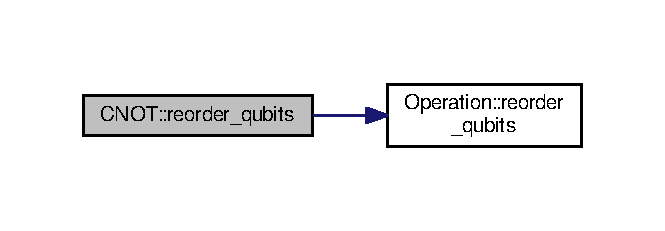
\includegraphics[width=319pt]{class_c_n_o_t_a2685ba9fe5fa414609a8ea6a9c2d18c7_cgraph}
\end{center}
\end{figure}




Here is the caller graph for this function\+:
\nopagebreak
\begin{figure}[H]
\begin{center}
\leavevmode
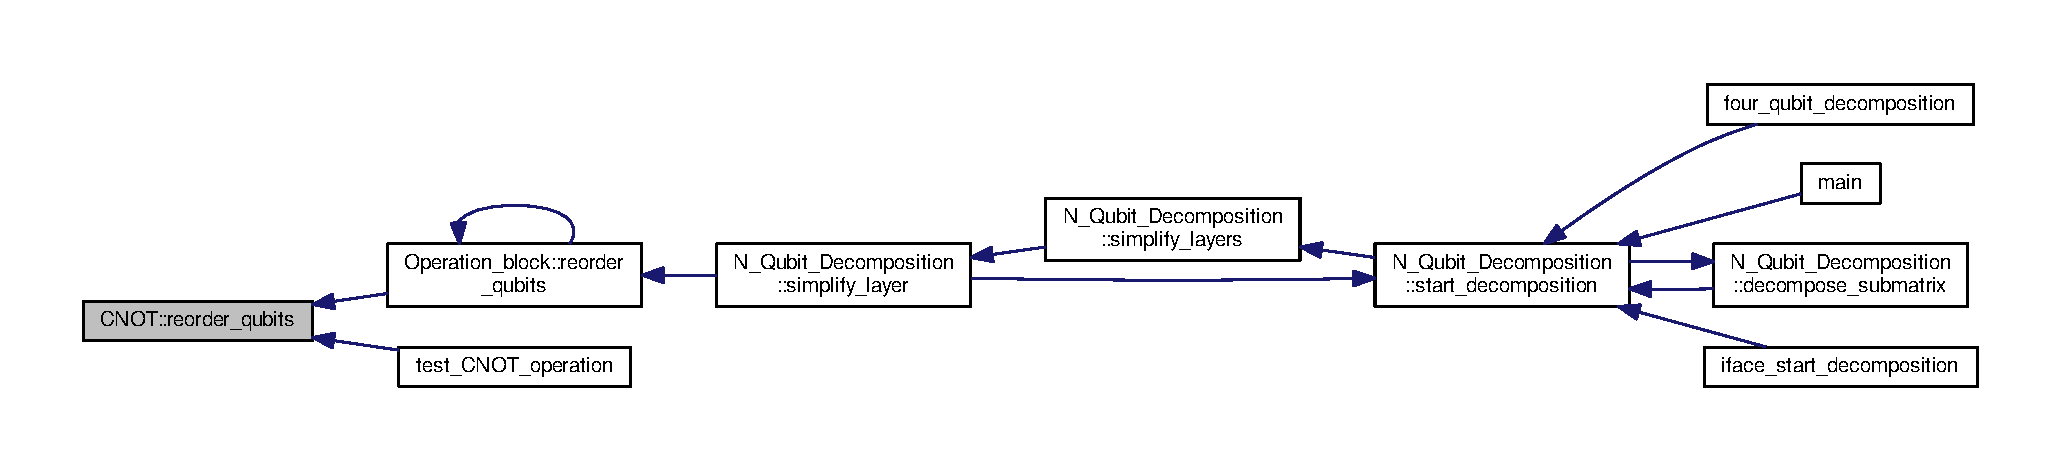
\includegraphics[width=350pt]{class_c_n_o_t_a2685ba9fe5fa414609a8ea6a9c2d18c7_icgraph}
\end{center}
\end{figure}


\index{C\+N\+OT@{C\+N\+OT}!set\+\_\+matrix@{set\+\_\+matrix}}
\index{set\+\_\+matrix@{set\+\_\+matrix}!C\+N\+OT@{C\+N\+OT}}
\subsubsection[{\texorpdfstring{set\+\_\+matrix(\+Q\+G\+D\+\_\+\+Complex16 $\ast$input)}{set_matrix(QGD_Complex16 *input)}}]{\setlength{\rightskip}{0pt plus 5cm}void Operation\+::set\+\_\+matrix (
\begin{DoxyParamCaption}
\item[{{\bf Q\+G\+D\+\_\+\+Complex16} $\ast$}]{input}
\end{DoxyParamCaption}
)\hspace{0.3cm}{\ttfamily [inherited]}}\hypertarget{class_operation_a026d3dcf0ad00af99c7a9097d3cf1c74}{}\label{class_operation_a026d3dcf0ad00af99c7a9097d3cf1c74}


Call to set the stored matrix in the operation. 


\begin{DoxyParams}{Parameters}
{\em input} & a pointer to the operation matrix to be stored. The matrix is copied into the storage pointed by . \\
\hline
\end{DoxyParams}
\begin{DoxyReturn}{Returns}
Returns with 0 on success. 
\end{DoxyReturn}
\index{C\+N\+OT@{C\+N\+OT}!set\+\_\+matrix@{set\+\_\+matrix}}
\index{set\+\_\+matrix@{set\+\_\+matrix}!C\+N\+OT@{C\+N\+OT}}
\subsubsection[{\texorpdfstring{set\+\_\+matrix(\+Q\+G\+D\+\_\+\+Complex16 $\ast$input)}{set_matrix(QGD_Complex16 *input)}}]{\setlength{\rightskip}{0pt plus 5cm}void Operation\+::set\+\_\+matrix (
\begin{DoxyParamCaption}
\item[{{\bf Q\+G\+D\+\_\+\+Complex16} $\ast$}]{input}
\end{DoxyParamCaption}
)\hspace{0.3cm}{\ttfamily [inherited]}}\hypertarget{class_operation_a026d3dcf0ad00af99c7a9097d3cf1c74}{}\label{class_operation_a026d3dcf0ad00af99c7a9097d3cf1c74}


Call to set the stored matrix in the operation. 


\begin{DoxyParams}{Parameters}
{\em input} & a pointer to the operation matrix to be stored. The matrix is copied into the storage pointed by . \\
\hline
\end{DoxyParams}
\begin{DoxyReturn}{Returns}
Returns with 0 on success. 
\end{DoxyReturn}


Definition at line 127 of file Operation.\+cpp.



Here is the call graph for this function\+:
\nopagebreak
\begin{figure}[H]
\begin{center}
\leavevmode
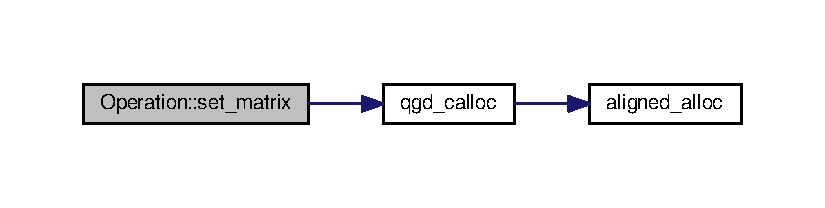
\includegraphics[width=350pt]{class_operation_a026d3dcf0ad00af99c7a9097d3cf1c74_cgraph}
\end{center}
\end{figure}




Here is the caller graph for this function\+:
\nopagebreak
\begin{figure}[H]
\begin{center}
\leavevmode
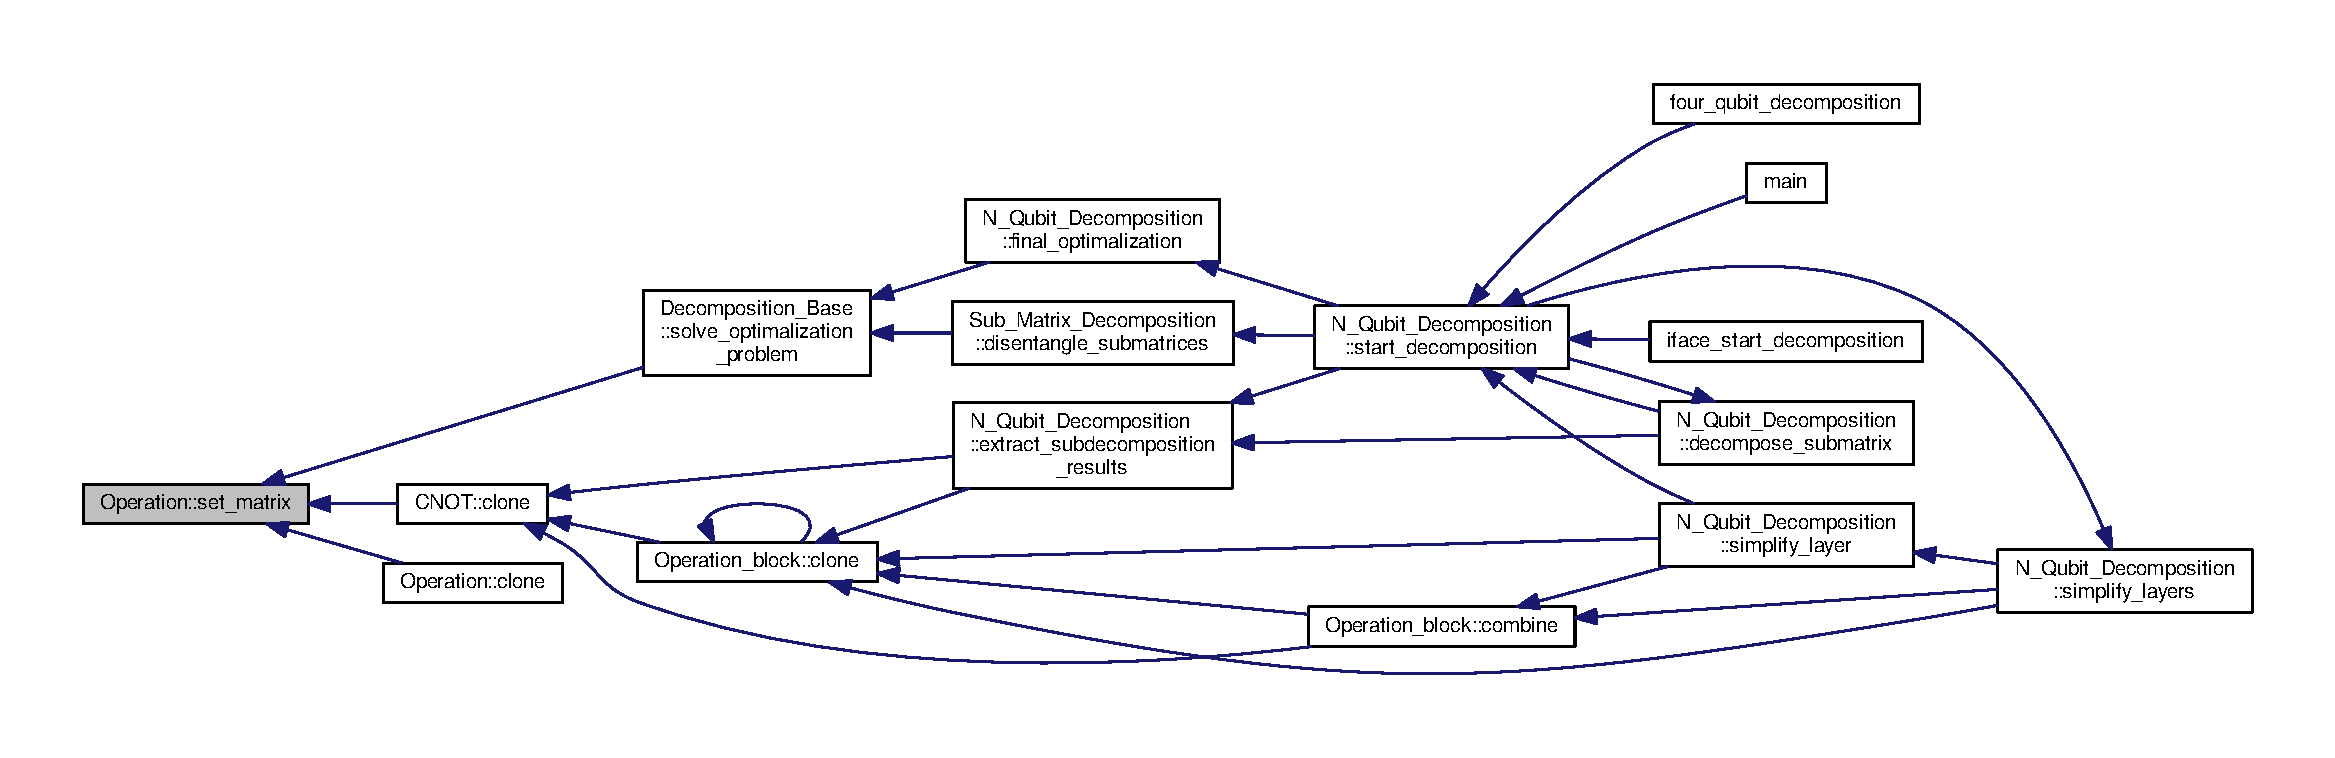
\includegraphics[width=350pt]{class_operation_a026d3dcf0ad00af99c7a9097d3cf1c74_icgraph}
\end{center}
\end{figure}


\index{C\+N\+OT@{C\+N\+OT}!set\+\_\+qbit\+\_\+num@{set\+\_\+qbit\+\_\+num}}
\index{set\+\_\+qbit\+\_\+num@{set\+\_\+qbit\+\_\+num}!C\+N\+OT@{C\+N\+OT}}
\subsubsection[{\texorpdfstring{set\+\_\+qbit\+\_\+num(int qbit\+\_\+num)}{set_qbit_num(int qbit_num)}}]{\setlength{\rightskip}{0pt plus 5cm}void C\+N\+O\+T\+::set\+\_\+qbit\+\_\+num (
\begin{DoxyParamCaption}
\item[{int}]{qbit\+\_\+num}
\end{DoxyParamCaption}
)\hspace{0.3cm}{\ttfamily [virtual]}}\hypertarget{class_c_n_o_t_a8272bf6e7ce6705a87d1ae9ef1e09418}{}\label{class_c_n_o_t_a8272bf6e7ce6705a87d1ae9ef1e09418}


Call to set the number of qubits spanning the matrix of the operation. 


\begin{DoxyParams}{Parameters}
{\em qbit\+\_\+num} & The number of qubits \\
\hline
\end{DoxyParams}


Reimplemented from \hyperlink{class_operation_ac107f65f10f3064e64372d4d17f2ff9b}{Operation}.

\index{C\+N\+OT@{C\+N\+OT}!set\+\_\+qbit\+\_\+num@{set\+\_\+qbit\+\_\+num}}
\index{set\+\_\+qbit\+\_\+num@{set\+\_\+qbit\+\_\+num}!C\+N\+OT@{C\+N\+OT}}
\subsubsection[{\texorpdfstring{set\+\_\+qbit\+\_\+num(int qbit\+\_\+num)}{set_qbit_num(int qbit_num)}}]{\setlength{\rightskip}{0pt plus 5cm}void C\+N\+O\+T\+::set\+\_\+qbit\+\_\+num (
\begin{DoxyParamCaption}
\item[{int}]{qbit\+\_\+num\+\_\+in}
\end{DoxyParamCaption}
)\hspace{0.3cm}{\ttfamily [virtual]}}\hypertarget{class_c_n_o_t_a8272bf6e7ce6705a87d1ae9ef1e09418}{}\label{class_c_n_o_t_a8272bf6e7ce6705a87d1ae9ef1e09418}


Call to set the number of qubits spanning the matrix of the operation. 


\begin{DoxyParams}{Parameters}
{\em qbit\+\_\+num} & The number of qubits \\
\hline
\end{DoxyParams}


Reimplemented from \hyperlink{class_operation_ac107f65f10f3064e64372d4d17f2ff9b}{Operation}.



Definition at line 190 of file C\+N\+O\+T.\+cpp.



Here is the call graph for this function\+:
\nopagebreak
\begin{figure}[H]
\begin{center}
\leavevmode
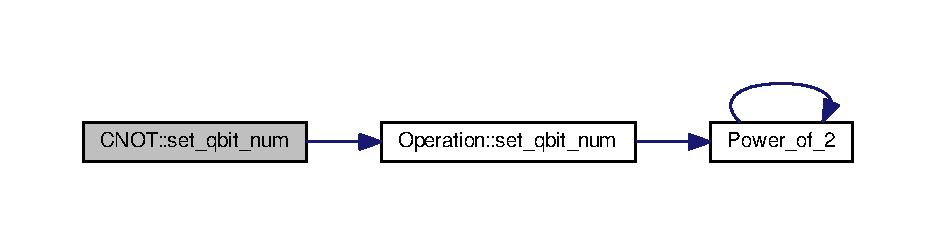
\includegraphics[width=350pt]{class_c_n_o_t_a8272bf6e7ce6705a87d1ae9ef1e09418_cgraph}
\end{center}
\end{figure}




Here is the caller graph for this function\+:
\nopagebreak
\begin{figure}[H]
\begin{center}
\leavevmode
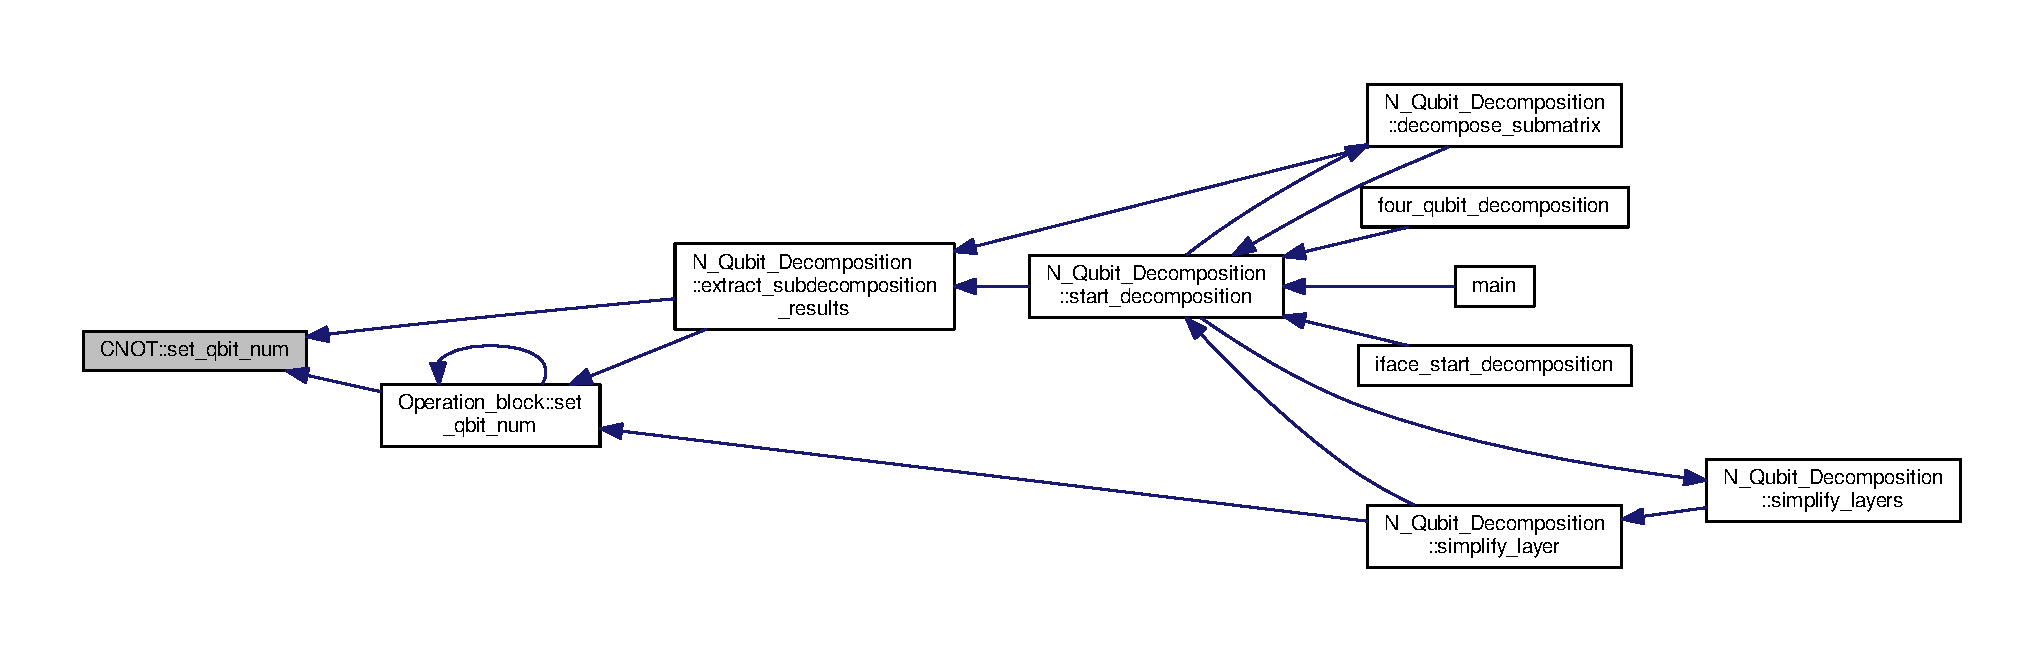
\includegraphics[width=350pt]{class_c_n_o_t_a8272bf6e7ce6705a87d1ae9ef1e09418_icgraph}
\end{center}
\end{figure}




\subsection{Member Data Documentation}
\index{C\+N\+OT@{C\+N\+OT}!control\+\_\+qbit@{control\+\_\+qbit}}
\index{control\+\_\+qbit@{control\+\_\+qbit}!C\+N\+OT@{C\+N\+OT}}
\subsubsection[{\texorpdfstring{control\+\_\+qbit}{control_qbit}}]{\setlength{\rightskip}{0pt plus 5cm}int Operation\+::control\+\_\+qbit\hspace{0.3cm}{\ttfamily [protected]}, {\ttfamily [inherited]}}\hypertarget{class_operation_a9a798ea8adec5a45fd2ca07996da88e1}{}\label{class_operation_a9a798ea8adec5a45fd2ca07996da88e1}


The index of the qubit which acts as a control qubit (control\+\_\+qbit $>$= 0) in controlled operations. 



Definition at line 54 of file operations/include/\+Operation.\+h.

\index{C\+N\+OT@{C\+N\+OT}!matrix\+\_\+alloc@{matrix\+\_\+alloc}}
\index{matrix\+\_\+alloc@{matrix\+\_\+alloc}!C\+N\+OT@{C\+N\+OT}}
\subsubsection[{\texorpdfstring{matrix\+\_\+alloc}{matrix_alloc}}]{\setlength{\rightskip}{0pt plus 5cm}{\bf Q\+G\+D\+\_\+\+Complex16} $\ast$ Operation\+::matrix\+\_\+alloc\hspace{0.3cm}{\ttfamily [protected]}, {\ttfamily [inherited]}}\hypertarget{class_operation_ade4d28d271ca13950d04363aac1c382e}{}\label{class_operation_ade4d28d271ca13950d04363aac1c382e}


Pointer to the operatrion matrix (if it is a constant general matrix) 



Definition at line 58 of file operations/include/\+Operation.\+h.

\index{C\+N\+OT@{C\+N\+OT}!matrix\+\_\+size@{matrix\+\_\+size}}
\index{matrix\+\_\+size@{matrix\+\_\+size}!C\+N\+OT@{C\+N\+OT}}
\subsubsection[{\texorpdfstring{matrix\+\_\+size}{matrix_size}}]{\setlength{\rightskip}{0pt plus 5cm}int Operation\+::matrix\+\_\+size\hspace{0.3cm}{\ttfamily [protected]}, {\ttfamily [inherited]}}\hypertarget{class_operation_a8236c07112cb165a00d3869363808624}{}\label{class_operation_a8236c07112cb165a00d3869363808624}


The size N of the NxN matrix associated with the operations. 



Definition at line 56 of file operations/include/\+Operation.\+h.

\index{C\+N\+OT@{C\+N\+OT}!parameter\+\_\+num@{parameter\+\_\+num}}
\index{parameter\+\_\+num@{parameter\+\_\+num}!C\+N\+OT@{C\+N\+OT}}
\subsubsection[{\texorpdfstring{parameter\+\_\+num}{parameter_num}}]{\setlength{\rightskip}{0pt plus 5cm}int Operation\+::parameter\+\_\+num\hspace{0.3cm}{\ttfamily [protected]}, {\ttfamily [inherited]}}\hypertarget{class_operation_aa57505afe5b5ec27f6d053044b86e043}{}\label{class_operation_aa57505afe5b5ec27f6d053044b86e043}


the number of free parameters of the operation 



Definition at line 60 of file operations/include/\+Operation.\+h.

\index{C\+N\+OT@{C\+N\+OT}!qbit\+\_\+num@{qbit\+\_\+num}}
\index{qbit\+\_\+num@{qbit\+\_\+num}!C\+N\+OT@{C\+N\+OT}}
\subsubsection[{\texorpdfstring{qbit\+\_\+num}{qbit_num}}]{\setlength{\rightskip}{0pt plus 5cm}int Operation\+::qbit\+\_\+num\hspace{0.3cm}{\ttfamily [protected]}, {\ttfamily [inherited]}}\hypertarget{class_operation_aecd5fbf1dd4ea532b2e58471ff8bad69}{}\label{class_operation_aecd5fbf1dd4ea532b2e58471ff8bad69}


number of qubits spanning the matrix of the operation 



Definition at line 48 of file operations/include/\+Operation.\+h.

\index{C\+N\+OT@{C\+N\+OT}!target\+\_\+qbit@{target\+\_\+qbit}}
\index{target\+\_\+qbit@{target\+\_\+qbit}!C\+N\+OT@{C\+N\+OT}}
\subsubsection[{\texorpdfstring{target\+\_\+qbit}{target_qbit}}]{\setlength{\rightskip}{0pt plus 5cm}int Operation\+::target\+\_\+qbit\hspace{0.3cm}{\ttfamily [protected]}, {\ttfamily [inherited]}}\hypertarget{class_operation_a3e489b72c124b494777c71b1646bb1e9}{}\label{class_operation_a3e489b72c124b494777c71b1646bb1e9}


The index of the qubit on which the operation acts (target\+\_\+qbit $>$= 0) 



Definition at line 52 of file operations/include/\+Operation.\+h.

\index{C\+N\+OT@{C\+N\+OT}!type@{type}}
\index{type@{type}!C\+N\+OT@{C\+N\+OT}}
\subsubsection[{\texorpdfstring{type}{type}}]{\setlength{\rightskip}{0pt plus 5cm}{\bf operation\+\_\+type} Operation\+::type\hspace{0.3cm}{\ttfamily [protected]}, {\ttfamily [inherited]}}\hypertarget{class_operation_ad47c56c86d62a4c775571e1600416479}{}\label{class_operation_ad47c56c86d62a4c775571e1600416479}


The type of the operation (see enumeration operation\+\_\+type) 



Definition at line 50 of file operations/include/\+Operation.\+h.



The documentation for this class was generated from the following files\+:\begin{DoxyCompactItemize}
\item 
\hyperlink{operations_2include_2_c_n_o_t_8h}{operations/include/\+C\+N\+O\+T.\+h}\item 
\hyperlink{_c_n_o_t_8cpp}{C\+N\+O\+T.\+cpp}\end{DoxyCompactItemize}

\hypertarget{class_decomposition___base}{}\section{Decomposition\+\_\+\+Base Class Reference}
\label{class_decomposition___base}\index{Decomposition\+\_\+\+Base@{Decomposition\+\_\+\+Base}}


A class containing basic methods for the decomposition process.  




{\ttfamily \#include $<$Decomposition\+\_\+\+Base.\+h$>$}



Inheritance diagram for Decomposition\+\_\+\+Base\+:
\nopagebreak
\begin{figure}[H]
\begin{center}
\leavevmode
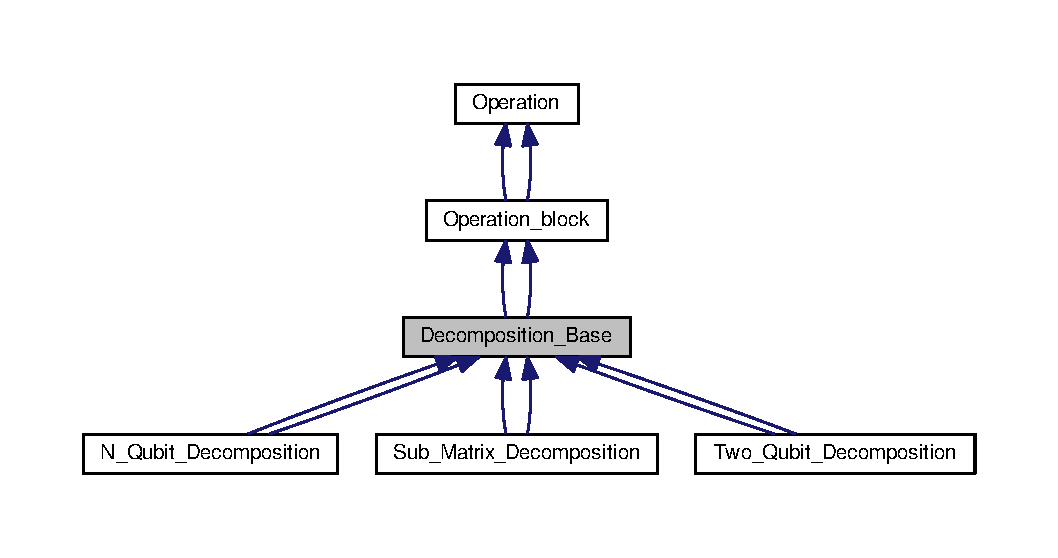
\includegraphics[width=350pt]{class_decomposition___base__inherit__graph}
\end{center}
\end{figure}
\subsection*{Public Member Functions}
\begin{DoxyCompactItemize}
\item 
void \hyperlink{class_operation__block_a3779e559654f12c5544129c46305b6ce}{add\+\_\+cnot\+\_\+to\+\_\+end} (int \hyperlink{class_operation_a9a798ea8adec5a45fd2ca07996da88e1}{control\+\_\+qbit}, int \hyperlink{class_operation_a3e489b72c124b494777c71b1646bb1e9}{target\+\_\+qbit})
\begin{DoxyCompactList}\small\item\em Append a C\+\_\+\+N\+OT gate operation to the list of operations. \end{DoxyCompactList}\item 
void \hyperlink{class_operation__block_a3779e559654f12c5544129c46305b6ce}{add\+\_\+cnot\+\_\+to\+\_\+end} (int \hyperlink{class_operation_a9a798ea8adec5a45fd2ca07996da88e1}{control\+\_\+qbit}, int \hyperlink{class_operation_a3e489b72c124b494777c71b1646bb1e9}{target\+\_\+qbit})
\begin{DoxyCompactList}\small\item\em Append a C\+\_\+\+N\+OT gate operation to the list of operations. \end{DoxyCompactList}\item 
void \hyperlink{class_operation__block_a207dfeddc26d79125a58e2c282bb0987}{add\+\_\+cnot\+\_\+to\+\_\+front} (int \hyperlink{class_operation_a9a798ea8adec5a45fd2ca07996da88e1}{control\+\_\+qbit}, int \hyperlink{class_operation_a3e489b72c124b494777c71b1646bb1e9}{target\+\_\+qbit})
\begin{DoxyCompactList}\small\item\em Add a C\+\_\+\+N\+OT gate operation to the front of the list of operations. \end{DoxyCompactList}\item 
void \hyperlink{class_operation__block_a207dfeddc26d79125a58e2c282bb0987}{add\+\_\+cnot\+\_\+to\+\_\+front} (int \hyperlink{class_operation_a9a798ea8adec5a45fd2ca07996da88e1}{control\+\_\+qbit}, int \hyperlink{class_operation_a3e489b72c124b494777c71b1646bb1e9}{target\+\_\+qbit})
\begin{DoxyCompactList}\small\item\em Add a C\+\_\+\+N\+OT gate operation to the front of the list of operations. \end{DoxyCompactList}\item 
void \hyperlink{class_operation__block_a0048efcfca374a6b960a1092ab564f03}{add\+\_\+operation\+\_\+to\+\_\+end} (\hyperlink{class_operation}{Operation} $\ast$operation)
\begin{DoxyCompactList}\small\item\em Append a general operation to the list of operations. \end{DoxyCompactList}\item 
void \hyperlink{class_operation__block_a0048efcfca374a6b960a1092ab564f03}{add\+\_\+operation\+\_\+to\+\_\+end} (\hyperlink{class_operation}{Operation} $\ast$operation)
\begin{DoxyCompactList}\small\item\em Append a general operation to the list of operations. \end{DoxyCompactList}\item 
void \hyperlink{class_operation__block_a1db22aed1f33a97bcaa2fad8c321a243}{add\+\_\+operation\+\_\+to\+\_\+front} (\hyperlink{class_operation}{Operation} $\ast$operation)
\begin{DoxyCompactList}\small\item\em Add an operation to the front of the list of operations. \end{DoxyCompactList}\item 
void \hyperlink{class_operation__block_a1db22aed1f33a97bcaa2fad8c321a243}{add\+\_\+operation\+\_\+to\+\_\+front} (\hyperlink{class_operation}{Operation} $\ast$operation)
\begin{DoxyCompactList}\small\item\em Add an operation to the front of the list of operations. \end{DoxyCompactList}\item 
void \hyperlink{class_operation__block_a2253d0a652bdce52a53d45e6d0a41abd}{add\+\_\+operations\+\_\+to\+\_\+end} (vector$<$ \hyperlink{class_operation}{Operation} $\ast$ $>$ operations\+\_\+in)
\begin{DoxyCompactList}\small\item\em Append a list of operations to the list of operations. \end{DoxyCompactList}\item 
void \hyperlink{class_operation__block_a2253d0a652bdce52a53d45e6d0a41abd}{add\+\_\+operations\+\_\+to\+\_\+end} (vector$<$ \hyperlink{class_operation}{Operation} $\ast$ $>$ operations\+\_\+in)
\begin{DoxyCompactList}\small\item\em Append a list of operations to the list of operations. \end{DoxyCompactList}\item 
void \hyperlink{class_operation__block_a50210aa57a18243de26631e0f6f823b6}{add\+\_\+operations\+\_\+to\+\_\+front} (vector$<$ \hyperlink{class_operation}{Operation} $\ast$ $>$ operations\+\_\+in)
\begin{DoxyCompactList}\small\item\em Add an array of operations to the front of the list of operations. \end{DoxyCompactList}\item 
void \hyperlink{class_operation__block_a50210aa57a18243de26631e0f6f823b6}{add\+\_\+operations\+\_\+to\+\_\+front} (vector$<$ \hyperlink{class_operation}{Operation} $\ast$ $>$ operations\+\_\+in)
\begin{DoxyCompactList}\small\item\em Add an array of operations to the front of the list of operations. \end{DoxyCompactList}\item 
void \hyperlink{class_operation__block_a44940209dbc5754b676b5a493bb153f4}{add\+\_\+u3\+\_\+to\+\_\+end} (int \hyperlink{class_operation_a3e489b72c124b494777c71b1646bb1e9}{target\+\_\+qbit}, bool Theta, bool Phi, bool Lambda)
\begin{DoxyCompactList}\small\item\em Append a \hyperlink{class_u3}{U3} gate to the list of operations. \end{DoxyCompactList}\item 
void \hyperlink{class_operation__block_a44940209dbc5754b676b5a493bb153f4}{add\+\_\+u3\+\_\+to\+\_\+end} (int \hyperlink{class_operation_a3e489b72c124b494777c71b1646bb1e9}{target\+\_\+qbit}, bool Theta, bool Phi, bool Lambda)
\begin{DoxyCompactList}\small\item\em Append a \hyperlink{class_u3}{U3} gate to the list of operations. \end{DoxyCompactList}\item 
void \hyperlink{class_operation__block_ac870a2afab73fa33f706e2e35829b452}{add\+\_\+u3\+\_\+to\+\_\+front} (int \hyperlink{class_operation_a3e489b72c124b494777c71b1646bb1e9}{target\+\_\+qbit}, bool Theta, bool Phi, bool Lambda)
\begin{DoxyCompactList}\small\item\em Add a \hyperlink{class_u3}{U3} gate to the front of the list of operations. \end{DoxyCompactList}\item 
void \hyperlink{class_operation__block_ac870a2afab73fa33f706e2e35829b452}{add\+\_\+u3\+\_\+to\+\_\+front} (int \hyperlink{class_operation_a3e489b72c124b494777c71b1646bb1e9}{target\+\_\+qbit}, bool Theta, bool Phi, bool Lambda)
\begin{DoxyCompactList}\small\item\em Add a \hyperlink{class_u3}{U3} gate to the front of the list of operations. \end{DoxyCompactList}\item 
\hyperlink{struct_q_g_d___complex16}{Q\+G\+D\+\_\+\+Complex16} $\ast$ \hyperlink{class_decomposition___base_a07d2b71ccdf4925377ee18bc552bb257}{apply\+\_\+operation} (\hyperlink{struct_q_g_d___complex16}{Q\+G\+D\+\_\+\+Complex16} $\ast$operation\+\_\+mtx, \hyperlink{struct_q_g_d___complex16}{Q\+G\+D\+\_\+\+Complex16} $\ast$input\+\_\+matrix)
\begin{DoxyCompactList}\small\item\em Apply an operations on the input matrix. \end{DoxyCompactList}\item 
\hyperlink{struct_q_g_d___complex16}{Q\+G\+D\+\_\+\+Complex16} $\ast$ \hyperlink{class_decomposition___base_a4963d3fe033c225eb19a0e6f271ef37a}{apply\+\_\+operation} (\hyperlink{struct_q_g_d___complex16}{Q\+G\+D\+\_\+\+Complex16} $\ast$operation\+\_\+mtx, \hyperlink{struct_q_g_d___complex16}{Q\+G\+D\+\_\+\+Complex16} $\ast$input\+\_\+matrix)
\begin{DoxyCompactList}\small\item\em Apply an operations on the input matrix. \end{DoxyCompactList}\item 
int \hyperlink{class_decomposition___base_aa6d12ac493c26af71613bc570fb87858}{apply\+\_\+operation} (\hyperlink{struct_q_g_d___complex16}{Q\+G\+D\+\_\+\+Complex16} $\ast$operation\+\_\+mtx, \hyperlink{struct_q_g_d___complex16}{Q\+G\+D\+\_\+\+Complex16} $\ast$input\+\_\+matrix, \hyperlink{struct_q_g_d___complex16}{Q\+G\+D\+\_\+\+Complex16} $\ast$result\+\_\+matrix)
\begin{DoxyCompactList}\small\item\em Apply an operations on the input matrix. \end{DoxyCompactList}\item 
int \hyperlink{class_decomposition___base_aa6d12ac493c26af71613bc570fb87858}{apply\+\_\+operation} (\hyperlink{struct_q_g_d___complex16}{Q\+G\+D\+\_\+\+Complex16} $\ast$operation\+\_\+mtx, \hyperlink{struct_q_g_d___complex16}{Q\+G\+D\+\_\+\+Complex16} $\ast$input\+\_\+matrix, \hyperlink{struct_q_g_d___complex16}{Q\+G\+D\+\_\+\+Complex16} $\ast$result\+\_\+matrix)
\begin{DoxyCompactList}\small\item\em Apply an operations on the input matrix. \end{DoxyCompactList}\item 
bool \hyperlink{class_decomposition___base_aa01a8d70b76215a235cb0d71894b2595}{check\+\_\+optimalization\+\_\+solution} ()
\begin{DoxyCompactList}\small\item\em check\+\_\+optimalization\+\_\+solution \end{DoxyCompactList}\item 
bool \hyperlink{class_decomposition___base_aa01a8d70b76215a235cb0d71894b2595}{check\+\_\+optimalization\+\_\+solution} ()
\begin{DoxyCompactList}\small\item\em check\+\_\+optimalization\+\_\+solution \end{DoxyCompactList}\item 
\hyperlink{class_operation__block}{Operation\+\_\+block} $\ast$ \hyperlink{class_operation__block_a2aa75d20b21c3b5802730c0abe54db5e}{clone} ()
\begin{DoxyCompactList}\small\item\em Create a clone of the present class. \end{DoxyCompactList}\item 
\hyperlink{class_operation__block}{Operation\+\_\+block} $\ast$ \hyperlink{class_operation__block_af5d1f81be3a54eada1de293d1e9877c5}{clone} ()
\begin{DoxyCompactList}\small\item\em Create a clone of the present class. \end{DoxyCompactList}\item 
void \hyperlink{class_operation__block_a60062cf6f48ebfdcaae9db3367a66147}{combine} (\hyperlink{class_operation__block}{Operation\+\_\+block} $\ast$op\+\_\+block)
\begin{DoxyCompactList}\small\item\em Call to append the operations of an operation block to the current block. \end{DoxyCompactList}\item 
void \hyperlink{class_operation__block_a60062cf6f48ebfdcaae9db3367a66147}{combine} (\hyperlink{class_operation__block}{Operation\+\_\+block} $\ast$op\+\_\+block)
\begin{DoxyCompactList}\small\item\em Call to append the operations of an operation block to the current block. \end{DoxyCompactList}\item 
\hyperlink{class_decomposition___base_a1f3d192d35a7154ac02e2bb3de80cd45}{Decomposition\+\_\+\+Base} (\hyperlink{struct_q_g_d___complex16}{Q\+G\+D\+\_\+\+Complex16} $\ast$Umtx\+\_\+in, int qbit\+\_\+num\+\_\+in, \hyperlink{decomposition_2include_2_decomposition___base_8h_a0e76cf2e4eb5edbf067ba5014ffa2134}{guess\+\_\+type} initial\+\_\+guess\+\_\+in)
\begin{DoxyCompactList}\small\item\em Contructor of the class. \end{DoxyCompactList}\item 
\hyperlink{class_decomposition___base_a1f3d192d35a7154ac02e2bb3de80cd45}{Decomposition\+\_\+\+Base} (\hyperlink{struct_q_g_d___complex16}{Q\+G\+D\+\_\+\+Complex16} $\ast$Umtx\+\_\+in, int qbit\+\_\+num\+\_\+in, \hyperlink{decomposition_2include_2_decomposition___base_8h_a0e76cf2e4eb5edbf067ba5014ffa2134}{guess\+\_\+type} initial\+\_\+guess\+\_\+in)
\begin{DoxyCompactList}\small\item\em Contructor of the class. \end{DoxyCompactList}\item 
void \hyperlink{class_decomposition___base_a0cdd12741e72e2c074a188fe3867e6d5}{finalize\+\_\+decomposition} ()
\begin{DoxyCompactList}\small\item\em After the main optimalization problem is solved, the indepent qubits can be rotated into state $\vert$0$>$ by this def. \end{DoxyCompactList}\item 
void \hyperlink{class_decomposition___base_a0cdd12741e72e2c074a188fe3867e6d5}{finalize\+\_\+decomposition} ()
\begin{DoxyCompactList}\small\item\em After the main optimalization problem is solved, the indepent qubits can be rotated into state $\vert$0$>$ by this def. \end{DoxyCompactList}\item 
int \hyperlink{class_operation_a2e9b60d334a0e0c99dede014ac989d0a}{get\+\_\+control\+\_\+qbit} ()
\begin{DoxyCompactList}\small\item\em Call to get the index of the control qubit. \end{DoxyCompactList}\item 
int \hyperlink{class_operation_a2e9b60d334a0e0c99dede014ac989d0a}{get\+\_\+control\+\_\+qbit} ()
\begin{DoxyCompactList}\small\item\em Call to get the index of the control qubit. \end{DoxyCompactList}\item 
\hyperlink{struct_q_g_d___complex16}{Q\+G\+D\+\_\+\+Complex16} $\ast$ \hyperlink{class_decomposition___base_ae71eaec68c77e79716cae632f97d42eb}{get\+\_\+decomposed\+\_\+matrix} ()
\begin{DoxyCompactList}\small\item\em Calculate the decomposed matrix resulted by the effect of the optimized operations on the unitary . \end{DoxyCompactList}\item 
\hyperlink{struct_q_g_d___complex16}{Q\+G\+D\+\_\+\+Complex16} $\ast$ \hyperlink{class_decomposition___base_a40154345dce69fd5a9cb28c0b677746b}{get\+\_\+decomposed\+\_\+matrix} ()
\begin{DoxyCompactList}\small\item\em Calculate the decomposed matrix resulted by the effect of the optimized operations on the unitary . \end{DoxyCompactList}\item 
void \hyperlink{class_decomposition___base_a9832cc5308c00b73d3e6bc331a77c7f7}{get\+\_\+finalizing\+\_\+operations} (\hyperlink{struct_q_g_d___complex16}{Q\+G\+D\+\_\+\+Complex16} $\ast$mtx, \hyperlink{class_operation__block}{Operation\+\_\+block} $\ast$finalizing\+\_\+operations, double $\ast$finalizing\+\_\+parameters)
\begin{DoxyCompactList}\small\item\em This method determine the operations needed to rotate the indepent qubits into the state $\vert$0$>$ \end{DoxyCompactList}\item 
void \hyperlink{class_decomposition___base_a9832cc5308c00b73d3e6bc331a77c7f7}{get\+\_\+finalizing\+\_\+operations} (\hyperlink{struct_q_g_d___complex16}{Q\+G\+D\+\_\+\+Complex16} $\ast$mtx, \hyperlink{class_operation__block}{Operation\+\_\+block} $\ast$finalizing\+\_\+operations, double $\ast$finalizing\+\_\+parameters)
\begin{DoxyCompactList}\small\item\em This method determine the operations needed to rotate the indepent qubits into the state $\vert$0$>$ \end{DoxyCompactList}\item 
\hyperlink{structgates__num}{gates\+\_\+num} \hyperlink{class_operation__block_ac39ab782da3e34c8ec4acf6181fbc5f7}{get\+\_\+gate\+\_\+nums} ()
\begin{DoxyCompactList}\small\item\em Call to get the number of the individual gate types in the list of operations. \end{DoxyCompactList}\item 
\hyperlink{structgates__num}{gates\+\_\+num} \hyperlink{class_operation__block_ac39ab782da3e34c8ec4acf6181fbc5f7}{get\+\_\+gate\+\_\+nums} ()
\begin{DoxyCompactList}\small\item\em Call to get the number of the individual gate types in the list of operations. \end{DoxyCompactList}\item 
std\+::vector$<$ int $>$ \hyperlink{class_operation__block_a92e4f0566e4b36830652729377a8e936}{get\+\_\+involved\+\_\+qubits} ()
\begin{DoxyCompactList}\small\item\em Call to get the qubits involved in the operations stored in the block of operations. \end{DoxyCompactList}\item 
std\+::vector$<$ int $>$ \hyperlink{class_operation__block_aebdbb71e02ff6826d967d55f4cd4db28}{get\+\_\+involved\+\_\+qubits} ()
\begin{DoxyCompactList}\small\item\em Call to get the qubits involved in the operations stored in the block of operations. \end{DoxyCompactList}\item 
std\+::vector$<$ \hyperlink{struct_q_g_d___complex16}{Q\+G\+D\+\_\+\+Complex16} $\ast$ $>$ \hyperlink{class_operation__block_af3e794fd9a409978a414af539ad23320}{get\+\_\+matrices} (const double $\ast$parameters)
\begin{DoxyCompactList}\small\item\em Call to get the list of matrix representation of the operations grouped in the block. \end{DoxyCompactList}\item 
std\+::vector$<$ \hyperlink{struct_q_g_d___complex16}{Q\+G\+D\+\_\+\+Complex16} $\ast$ $>$ \hyperlink{class_operation__block_aedddbc5242eab7c00125359a835ac53d}{get\+\_\+matrices} (const double $\ast$parameters)
\begin{DoxyCompactList}\small\item\em Call to get the list of matrix representation of the operations grouped in the block. \end{DoxyCompactList}\item 
int \hyperlink{class_decomposition___base_a64e2b692d38fe3ccbd49708d8fa24493}{get\+\_\+operation} (int n, \hyperlink{operations_2include_2_operation_8h_ad99e62941c8e4b13e5fc45ecaaf65eff}{operation\+\_\+type} \&\hyperlink{class_operation_ad47c56c86d62a4c775571e1600416479}{type}, int \&\hyperlink{class_operation_a3e489b72c124b494777c71b1646bb1e9}{target\+\_\+qbit}, int \&\hyperlink{class_operation_a9a798ea8adec5a45fd2ca07996da88e1}{control\+\_\+qbit}, double $\ast$parameters)
\begin{DoxyCompactList}\small\item\em Call to prepare the optimized operations to export. \end{DoxyCompactList}\item 
int \hyperlink{class_decomposition___base_a64e2b692d38fe3ccbd49708d8fa24493}{get\+\_\+operation} (int n, \hyperlink{operations_2include_2_operation_8h_ad99e62941c8e4b13e5fc45ecaaf65eff}{operation\+\_\+type} \&\hyperlink{class_operation_ad47c56c86d62a4c775571e1600416479}{type}, int \&\hyperlink{class_operation_a3e489b72c124b494777c71b1646bb1e9}{target\+\_\+qbit}, int \&\hyperlink{class_operation_a9a798ea8adec5a45fd2ca07996da88e1}{control\+\_\+qbit}, double $\ast$parameters)
\begin{DoxyCompactList}\small\item\em Call to prepare the optimized operations to export. \end{DoxyCompactList}\item 
int \hyperlink{class_operation__block_a27592a2d25c7e74416de2b9d7997efca}{get\+\_\+operation\+\_\+num} ()
\begin{DoxyCompactList}\small\item\em Call to get the number of operations grouped in the block. \end{DoxyCompactList}\item 
int \hyperlink{class_operation__block_a27592a2d25c7e74416de2b9d7997efca}{get\+\_\+operation\+\_\+num} ()
\begin{DoxyCompactList}\small\item\em Call to get the number of operations grouped in the block. \end{DoxyCompactList}\item 
std\+::vector$<$ \hyperlink{struct_q_g_d___complex16}{Q\+G\+D\+\_\+\+Complex16} $\ast$ $>$ \hyperlink{class_decomposition___base_a7e6efc3b157653de20275e234d4df3d9}{get\+\_\+operation\+\_\+products} (double $\ast$parameters, std\+::vector$<$ \hyperlink{class_operation}{Operation} $\ast$ $>$\+::iterator operations\+\_\+it, int num\+\_\+of\+\_\+operations)
\begin{DoxyCompactList}\small\item\em Calculate the list of gate operation matrices such that the i$>$0-\/th element in the result list is the product of the operations of all 0$<$=n$<$i operations from the input list and the 0th element in the result list is the identity. \end{DoxyCompactList}\item 
std\+::vector$<$ \hyperlink{struct_q_g_d___complex16}{Q\+G\+D\+\_\+\+Complex16} $\ast$ $>$ \hyperlink{class_decomposition___base_a7f3fd202c32e65cbc312ec61d426442a}{get\+\_\+operation\+\_\+products} (double $\ast$parameters, std\+::vector$<$ \hyperlink{class_operation}{Operation} $\ast$ $>$\+::iterator operations\+\_\+it, int num\+\_\+of\+\_\+operations)
\begin{DoxyCompactList}\small\item\em Calculate the list of gate operation matrices such that the i$>$0-\/th element in the result list is the product of the operations of all 0$<$=n$<$i operations from the input list and the 0th element in the result list is the identity. \end{DoxyCompactList}\item 
std\+::vector$<$ \hyperlink{class_operation}{Operation} $\ast$ $>$ \hyperlink{class_operation__block_a489d0c5758732ca49d5f5aca225e9318}{get\+\_\+operations} ()
\begin{DoxyCompactList}\small\item\em Call to get the operations stored in the block. \end{DoxyCompactList}\item 
std\+::vector$<$ \hyperlink{class_operation}{Operation} $\ast$ $>$ \hyperlink{class_operation__block_aecb9b674dfd43456605a6c13dfba3afb}{get\+\_\+operations} ()
\begin{DoxyCompactList}\small\item\em Call to get the operations stored in the block. \end{DoxyCompactList}\item 
double $\ast$ \hyperlink{class_decomposition___base_a27c8d07322621ccd644aaff8af667809}{get\+\_\+optimized\+\_\+parameters} ()
\begin{DoxyCompactList}\small\item\em Call to get the optimized parameters. \end{DoxyCompactList}\item 
double $\ast$ \hyperlink{class_decomposition___base_ae2dd23fc79127ca9d25eafeb1137d094}{get\+\_\+optimized\+\_\+parameters} ()
\begin{DoxyCompactList}\small\item\em Call to get the optimized parameters. \end{DoxyCompactList}\item 
void \hyperlink{class_decomposition___base_ae9d74e7137a05ceda5d6efeba8cc6c8e}{get\+\_\+optimized\+\_\+parameters} (double $\ast$ret)
\begin{DoxyCompactList}\small\item\em Call to get the optimized parameters. \end{DoxyCompactList}\item 
void \hyperlink{class_decomposition___base_ae9d74e7137a05ceda5d6efeba8cc6c8e}{get\+\_\+optimized\+\_\+parameters} (double $\ast$ret)
\begin{DoxyCompactList}\small\item\em Call to get the optimized parameters. \end{DoxyCompactList}\item 
int \hyperlink{class_operation__block_af7ff4a8876a7b1c062ea2f35efac18b0}{get\+\_\+parameter\+\_\+num} ()
\begin{DoxyCompactList}\small\item\em Call to get the number of free parameters. \end{DoxyCompactList}\item 
int \hyperlink{class_operation__block_af7ff4a8876a7b1c062ea2f35efac18b0}{get\+\_\+parameter\+\_\+num} ()
\begin{DoxyCompactList}\small\item\em Call to get the number of free parameters. \end{DoxyCompactList}\item 
int \hyperlink{class_operation_a55eee2ad4b90be085b1ec2ce018502f8}{get\+\_\+target\+\_\+qbit} ()
\begin{DoxyCompactList}\small\item\em Call to get the index of the target qubit. \end{DoxyCompactList}\item 
int \hyperlink{class_operation_a55eee2ad4b90be085b1ec2ce018502f8}{get\+\_\+target\+\_\+qbit} ()
\begin{DoxyCompactList}\small\item\em Call to get the index of the target qubit. \end{DoxyCompactList}\item 
\hyperlink{struct_q_g_d___complex16}{Q\+G\+D\+\_\+\+Complex16} $\ast$ \hyperlink{class_decomposition___base_a8e26f5a31475e4d5a2e9c785a2a57dd9}{get\+\_\+transformed\+\_\+matrix} (const double $\ast$parameters, std\+::vector$<$ \hyperlink{class_operation}{Operation} $\ast$ $>$\+::iterator \hyperlink{class_operation__block_a1efec4139888e591b59acd7b84497af1}{operations}, int num\+\_\+of\+\_\+operations, \hyperlink{struct_q_g_d___complex16}{Q\+G\+D\+\_\+\+Complex16} $\ast$initial\+\_\+matrix)
\begin{DoxyCompactList}\small\item\em Calculate the transformed matrix resulting by an array of operations on a given initial matrix. \end{DoxyCompactList}\item 
\hyperlink{struct_q_g_d___complex16}{Q\+G\+D\+\_\+\+Complex16} $\ast$ \hyperlink{class_decomposition___base_a74159036ee14ac2c33a0ccd45de782d5}{get\+\_\+transformed\+\_\+matrix} (const double $\ast$parameters, std\+::vector$<$ \hyperlink{class_operation}{Operation} $\ast$ $>$\+::iterator \hyperlink{class_operation__block_a1efec4139888e591b59acd7b84497af1}{operations}, int num\+\_\+of\+\_\+operations, \hyperlink{struct_q_g_d___complex16}{Q\+G\+D\+\_\+\+Complex16} $\ast$initial\+\_\+matrix)
\begin{DoxyCompactList}\small\item\em Calculate the transformed matrix resulting by an array of operations on a given initial matrix. \end{DoxyCompactList}\item 
\hyperlink{operations_2include_2_operation_8h_ad99e62941c8e4b13e5fc45ecaaf65eff}{operation\+\_\+type} \hyperlink{class_operation_acc601a7a00616fd6e2a61f61e084afac}{get\+\_\+type} ()
\begin{DoxyCompactList}\small\item\em Call to get the type of the operation. \end{DoxyCompactList}\item 
\hyperlink{operations_2include_2_operation_8h_ad99e62941c8e4b13e5fc45ecaaf65eff}{operation\+\_\+type} \hyperlink{class_operation_acc601a7a00616fd6e2a61f61e084afac}{get\+\_\+type} ()
\begin{DoxyCompactList}\small\item\em Call to get the type of the operation. \end{DoxyCompactList}\item 
\hyperlink{struct_q_g_d___complex16}{Q\+G\+D\+\_\+\+Complex16} $\ast$ \hyperlink{class_decomposition___base_a8375551739dde405c4e121ae0bbb09bf}{get\+\_\+\+Umtx} ()
\begin{DoxyCompactList}\small\item\em Call to retrive a pointer to the unitary to be transformed. \end{DoxyCompactList}\item 
\hyperlink{struct_q_g_d___complex16}{Q\+G\+D\+\_\+\+Complex16} $\ast$ \hyperlink{class_decomposition___base_ad1e8fca5e5710d3a59f10ed6c523a502}{get\+\_\+\+Umtx} ()
\begin{DoxyCompactList}\small\item\em Call to retrive a pointer to the unitary to be transformed. \end{DoxyCompactList}\item 
int \hyperlink{class_decomposition___base_a3a1f83b85fd9e7e67a89a79b8cdc1e4a}{get\+\_\+\+Umtx\+\_\+size} ()
\begin{DoxyCompactList}\small\item\em Call to get the size of the unitary to be transformed. \end{DoxyCompactList}\item 
int \hyperlink{class_decomposition___base_a3a1f83b85fd9e7e67a89a79b8cdc1e4a}{get\+\_\+\+Umtx\+\_\+size} ()
\begin{DoxyCompactList}\small\item\em Call to get the size of the unitary to be transformed. \end{DoxyCompactList}\item 
void \hyperlink{class_decomposition___base_a4c6c81d70f49ee249aa455a4f2718ee2}{list\+\_\+operations} (int start\+\_\+index)
\begin{DoxyCompactList}\small\item\em Call to print the operations decomposing the initial unitary. \end{DoxyCompactList}\item 
void \hyperlink{class_decomposition___base_a4c6c81d70f49ee249aa455a4f2718ee2}{list\+\_\+operations} (int start\+\_\+index)
\begin{DoxyCompactList}\small\item\em Call to print the operations decomposing the initial unitary. \end{DoxyCompactList}\item 
void \hyperlink{class_operation__block_a29e2c74d7fa7344193a17e39248eb803}{list\+\_\+operations} (const double $\ast$parameters, int start\+\_\+index)
\begin{DoxyCompactList}\small\item\em Call to print the list of operations stored in the block of operations for a specific set of parameters. \end{DoxyCompactList}\item 
\hyperlink{struct_q_g_d___complex16}{Q\+G\+D\+\_\+\+Complex16} $\ast$ \hyperlink{class_operation__block_a916db3ef5d6fcf25367843a1306cd4e0}{matrix} (const double $\ast$parameters)
\begin{DoxyCompactList}\small\item\em Call to retrieve the operation matrix (Which is the product of all the operation matrices stored in the operation block) \end{DoxyCompactList}\item 
\hyperlink{struct_q_g_d___complex16}{Q\+G\+D\+\_\+\+Complex16} $\ast$ \hyperlink{class_operation__block_a43cdb87a4ee2a339de30c94cc94fa40e}{matrix} (const double $\ast$parameters)
\begin{DoxyCompactList}\small\item\em Call to retrieve the operation matrix (Which is the product of all the operation matrices stored in the operation block) \end{DoxyCompactList}\item 
int \hyperlink{class_operation__block_abf4287a38eeca35a81163f86a361d95c}{matrix} (const double $\ast$parameters, \hyperlink{struct_q_g_d___complex16}{Q\+G\+D\+\_\+\+Complex16} $\ast$block\+\_\+mtx)
\begin{DoxyCompactList}\small\item\em Call to retrieve the operation matrix (Which is the product of all the operation matrices stored in the operation block) \end{DoxyCompactList}\item 
int \hyperlink{class_operation__block_abf4287a38eeca35a81163f86a361d95c}{matrix} (const double $\ast$parameters, \hyperlink{struct_q_g_d___complex16}{Q\+G\+D\+\_\+\+Complex16} $\ast$block\+\_\+mtx)
\begin{DoxyCompactList}\small\item\em Call to retrieve the operation matrix (Which is the product of all the operation matrices stored in the operation block) \end{DoxyCompactList}\item 
virtual \hyperlink{struct_q_g_d___complex16}{Q\+G\+D\+\_\+\+Complex16} $\ast$ \hyperlink{class_operation_acf7d1765143285ff73772ae860109988}{matrix} ()
\begin{DoxyCompactList}\small\item\em Call to terive the operation matrix. \end{DoxyCompactList}\item 
virtual int \hyperlink{class_operation_add11c6ea2626d8dbcbd00f328a8a8279}{matrix} (\hyperlink{struct_q_g_d___complex16}{Q\+G\+D\+\_\+\+Complex16} $\ast$retrieve\+\_\+matrix)
\begin{DoxyCompactList}\small\item\em Call to retrieve the operation matrix. \end{DoxyCompactList}\item 
virtual double \hyperlink{class_decomposition___base_abc06e307be293edcd0cecae99dfbed04}{optimalization\+\_\+problem} (const double $\ast$parameters)
\begin{DoxyCompactList}\small\item\em This is an abstact definition of function giving the cost functions measuring the entaglement of the qubits. \end{DoxyCompactList}\item 
virtual double \hyperlink{class_decomposition___base_a274b510011ebbc14c8acb67d844a5aef}{optimalization\+\_\+problem} (const double $\ast$parameters)
\begin{DoxyCompactList}\small\item\em This is an abstact definition of function giving the cost functions measuring the entaglement of the qubits. \end{DoxyCompactList}\item 
void \hyperlink{class_decomposition___base_a965838902240670119c0ad68d087c322}{prepare\+\_\+operations\+\_\+to\+\_\+export} ()
\begin{DoxyCompactList}\small\item\em Call to prepare the optimized operations to export. \end{DoxyCompactList}\item 
void \hyperlink{class_decomposition___base_a965838902240670119c0ad68d087c322}{prepare\+\_\+operations\+\_\+to\+\_\+export} ()
\begin{DoxyCompactList}\small\item\em Call to prepare the optimized operations to export. \end{DoxyCompactList}\item 
std\+::vector$<$ \hyperlink{class_operation}{Operation} $\ast$ $>$ \hyperlink{class_decomposition___base_a3efce739eaf575d284156813436bb469}{prepare\+\_\+operations\+\_\+to\+\_\+export} (std\+::vector$<$ \hyperlink{class_operation}{Operation} $\ast$ $>$ ops, const double $\ast$parameters)
\begin{DoxyCompactList}\small\item\em Call to prepare the optimized operations to export. \end{DoxyCompactList}\item 
std\+::vector$<$ \hyperlink{class_operation}{Operation} $\ast$ $>$ \hyperlink{class_decomposition___base_a68dcc2cdfa644cf8043021367cc07d28}{prepare\+\_\+operations\+\_\+to\+\_\+export} (std\+::vector$<$ \hyperlink{class_operation}{Operation} $\ast$ $>$ ops, const double $\ast$parameters)
\begin{DoxyCompactList}\small\item\em Call to prepare the optimized operations to export. \end{DoxyCompactList}\item 
std\+::vector$<$ \hyperlink{class_operation}{Operation} $\ast$ $>$ \hyperlink{class_decomposition___base_a267addf036c4207905f7f443aea471bb}{prepare\+\_\+operations\+\_\+to\+\_\+export} (\hyperlink{class_operation__block}{Operation\+\_\+block} $\ast$block\+\_\+op, const double $\ast$parameters)
\begin{DoxyCompactList}\small\item\em Call to prepare the operations of an operation block to export. \end{DoxyCompactList}\item 
std\+::vector$<$ \hyperlink{class_operation}{Operation} $\ast$ $>$ \hyperlink{class_decomposition___base_a9d4cf31a7409fcc6a74d6ed927839f15}{prepare\+\_\+operations\+\_\+to\+\_\+export} (\hyperlink{class_operation__block}{Operation\+\_\+block} $\ast$block\+\_\+op, const double $\ast$parameters)
\begin{DoxyCompactList}\small\item\em Call to prepare the operations of an operation block to export. \end{DoxyCompactList}\item 
void \hyperlink{class_operation__block_a7c3d4eadaef2f21f1c5dd9227faec7ce}{release\+\_\+operations} ()
\begin{DoxyCompactList}\small\item\em Call to release the stored operations. \end{DoxyCompactList}\item 
void \hyperlink{class_operation__block_a7c3d4eadaef2f21f1c5dd9227faec7ce}{release\+\_\+operations} ()
\begin{DoxyCompactList}\small\item\em Call to release the stored operations. \end{DoxyCompactList}\item 
void \hyperlink{class_operation__block_af2a71d29cdbce498e85f11b9ed81e0c9}{reorder\+\_\+qubits} (vector$<$ int $>$)
\begin{DoxyCompactList}\small\item\em Call to reorder the qubits in the matrix of the operation. \end{DoxyCompactList}\item 
void \hyperlink{class_operation__block_af2a71d29cdbce498e85f11b9ed81e0c9}{reorder\+\_\+qubits} (vector$<$ int $>$)
\begin{DoxyCompactList}\small\item\em Call to reorder the qubits in the matrix of the operation. \end{DoxyCompactList}\item 
int \hyperlink{class_decomposition___base_aaf2862ee2211dac36242551340190b4b}{set\+\_\+iteration\+\_\+loops} (int qbit, int iteration\+\_\+loops\+\_\+in)
\begin{DoxyCompactList}\small\item\em Set the number of iteration loops during the subdecomposition of the qbit-\/th qubit. \end{DoxyCompactList}\item 
int \hyperlink{class_decomposition___base_aaf2862ee2211dac36242551340190b4b}{set\+\_\+iteration\+\_\+loops} (int qbit, int iteration\+\_\+loops\+\_\+in)
\begin{DoxyCompactList}\small\item\em Set the number of iteration loops during the subdecomposition of the qbit-\/th qubit. \end{DoxyCompactList}\item 
int \hyperlink{class_decomposition___base_aa376f8cfdb1b9ed06bceff9c72ddf496}{set\+\_\+iteration\+\_\+loops} (std\+::map$<$ int, int $>$ iteration\+\_\+loops\+\_\+in)
\begin{DoxyCompactList}\small\item\em Set the number of iteration loops during the subdecomposition of the qbit-\/th qubit. \end{DoxyCompactList}\item 
int \hyperlink{class_decomposition___base_aa376f8cfdb1b9ed06bceff9c72ddf496}{set\+\_\+iteration\+\_\+loops} (std\+::map$<$ int, int $>$ iteration\+\_\+loops\+\_\+in)
\begin{DoxyCompactList}\small\item\em Set the number of iteration loops during the subdecomposition of the qbit-\/th qubit. \end{DoxyCompactList}\item 
void \hyperlink{class_operation_a026d3dcf0ad00af99c7a9097d3cf1c74}{set\+\_\+matrix} (\hyperlink{struct_q_g_d___complex16}{Q\+G\+D\+\_\+\+Complex16} $\ast$input)
\begin{DoxyCompactList}\small\item\em Call to set the stored matrix in the operation. \end{DoxyCompactList}\item 
void \hyperlink{class_operation_a026d3dcf0ad00af99c7a9097d3cf1c74}{set\+\_\+matrix} (\hyperlink{struct_q_g_d___complex16}{Q\+G\+D\+\_\+\+Complex16} $\ast$input)
\begin{DoxyCompactList}\small\item\em Call to set the stored matrix in the operation. \end{DoxyCompactList}\item 
void \hyperlink{class_decomposition___base_a26e98bca148157ec42e5f1618deb50ea}{set\+\_\+max\+\_\+iteration} (int \hyperlink{class_decomposition___base_a89e74f075626c21e23228772bf8ad395}{max\+\_\+iterations})
\begin{DoxyCompactList}\small\item\em Call to set the maximal number of the iterations in the optimalization process. \end{DoxyCompactList}\item 
void \hyperlink{class_decomposition___base_a26e98bca148157ec42e5f1618deb50ea}{set\+\_\+max\+\_\+iteration} (int \hyperlink{class_decomposition___base_a89e74f075626c21e23228772bf8ad395}{max\+\_\+iterations})
\begin{DoxyCompactList}\small\item\em Call to set the maximal number of the iterations in the optimalization process. \end{DoxyCompactList}\item 
int \hyperlink{class_decomposition___base_a6cbee8cd37f42b2fe6bdd6f5c0fd3fdb}{set\+\_\+max\+\_\+layer\+\_\+num} (int qbit, int max\+\_\+layer\+\_\+num\+\_\+in)
\begin{DoxyCompactList}\small\item\em Set the maximal number of layers used in the subdecomposition of the qbit-\/th qubit. \end{DoxyCompactList}\item 
int \hyperlink{class_decomposition___base_a6cbee8cd37f42b2fe6bdd6f5c0fd3fdb}{set\+\_\+max\+\_\+layer\+\_\+num} (int qbit, int max\+\_\+layer\+\_\+num\+\_\+in)
\begin{DoxyCompactList}\small\item\em Set the maximal number of layers used in the subdecomposition of the qbit-\/th qubit. \end{DoxyCompactList}\item 
void \hyperlink{class_decomposition___base_af3b3574285055f66f4769f6398a84745}{set\+\_\+optimalization\+\_\+blocks} (int)
\begin{DoxyCompactList}\small\item\em Call to set the number of operation blocks to be optimized in one shot. \end{DoxyCompactList}\item 
void \hyperlink{class_decomposition___base_af3b3574285055f66f4769f6398a84745}{set\+\_\+optimalization\+\_\+blocks} (int)
\begin{DoxyCompactList}\small\item\em Call to set the number of operation blocks to be optimized in one shot. \end{DoxyCompactList}\item 
void \hyperlink{class_operation__block_acc41ac933723558df3f4e65ae1158091}{set\+\_\+qbit\+\_\+num} (int qbit\+\_\+num\+\_\+in)
\begin{DoxyCompactList}\small\item\em Set the number of qubits spanning the matrix of the operations stored in the block of operations. \end{DoxyCompactList}\item 
void \hyperlink{class_operation__block_acc41ac933723558df3f4e65ae1158091}{set\+\_\+qbit\+\_\+num} (int qbit\+\_\+num\+\_\+in)
\begin{DoxyCompactList}\small\item\em Set the number of qubits spanning the matrix of the operations stored in the block of operations. \end{DoxyCompactList}\item 
virtual void \hyperlink{class_decomposition___base_acd8a90c71e28ddac71d0941b7d00acb7}{solve\+\_\+layer\+\_\+optimalization\+\_\+problem} (int num\+\_\+of\+\_\+parameters, gsl\+\_\+vector $\ast$solution\+\_\+guess\+\_\+gsl)
\begin{DoxyCompactList}\small\item\em Abstarct function to be used to solve a single sub-\/layer optimalization problem. \end{DoxyCompactList}\item 
virtual void \hyperlink{class_decomposition___base_af9e43f240238e3327e2701555a174ee4}{solve\+\_\+layer\+\_\+optimalization\+\_\+problem} (int num\+\_\+of\+\_\+parameters, gsl\+\_\+vector $\ast$solution\+\_\+guess\+\_\+gsl)
\begin{DoxyCompactList}\small\item\em Abstarct function to be used to solve a single sub-\/layer optimalization problem. \end{DoxyCompactList}\item 
void \hyperlink{class_decomposition___base_ae21ecd8c5016a6ec942330247e8cdebc}{solve\+\_\+optimalization\+\_\+problem} (double $\ast$solution\+\_\+guess, int solution\+\_\+guess\+\_\+num)
\begin{DoxyCompactList}\small\item\em This method can be used to solve the main optimalization problem which is devidid into sub-\/layer optimalization processes. \end{DoxyCompactList}\item 
void \hyperlink{class_decomposition___base_ae21ecd8c5016a6ec942330247e8cdebc}{solve\+\_\+optimalization\+\_\+problem} (double $\ast$solution\+\_\+guess, int solution\+\_\+guess\+\_\+num)
\begin{DoxyCompactList}\small\item\em This method can be used to solve the main optimalization problem which is devidid into sub-\/layer optimalization processes. \end{DoxyCompactList}\item 
\hyperlink{class_decomposition___base_ae0c67b0a277454c77e0b50e3dfd0ee84}{$\sim$\+Decomposition\+\_\+\+Base} ()
\begin{DoxyCompactList}\small\item\em Destructor of the class. \end{DoxyCompactList}\item 
\hyperlink{class_decomposition___base_ae0c67b0a277454c77e0b50e3dfd0ee84}{$\sim$\+Decomposition\+\_\+\+Base} ()
\begin{DoxyCompactList}\small\item\em Destructor of the class. \end{DoxyCompactList}\end{DoxyCompactItemize}
\subsection*{Static Public Member Functions}
\begin{DoxyCompactItemize}
\item 
static void \hyperlink{class_decomposition___base_a24c7d112a4f3b2346c3d885316f3bfa1}{Init\+\_\+max\+\_\+layer\+\_\+num} ()
\begin{DoxyCompactList}\small\item\em Initializes default layer numbers. \end{DoxyCompactList}\item 
static void \hyperlink{class_decomposition___base_abdb59c6b355a338eb958f58d6f28b966}{Init\+\_\+max\+\_\+layer\+\_\+num} ()
\begin{DoxyCompactList}\small\item\em Initializes default layer numbers. \end{DoxyCompactList}\end{DoxyCompactItemize}
\subsection*{Public Attributes}
\begin{DoxyCompactItemize}
\item 
int \hyperlink{class_decomposition___base_adae1205825aea9a9544d9ca42855b849}{optimalization\+\_\+block}
\begin{DoxyCompactList}\small\item\em number of operation blocks used in one shot of the optimalization process \end{DoxyCompactList}\item 
double \hyperlink{class_decomposition___base_ae08336b2cdfc58bbd03ba231716f28dd}{optimalization\+\_\+tolerance}
\begin{DoxyCompactList}\small\item\em The maximal allowed error of the optimalization problem. \end{DoxyCompactList}\item 
bool \hyperlink{class_decomposition___base_a0636a9e49a19f7167b7abdf309882042}{verbose}
\end{DoxyCompactItemize}
\subsection*{Static Public Attributes}
\begin{DoxyCompactItemize}
\item 
static std\+::map$<$ int, int $>$ \hyperlink{class_decomposition___base_a17952d9e72bbc214eb3a1466270b853d}{max\+\_\+layer\+\_\+num\+\_\+def}
\begin{DoxyCompactList}\small\item\em A map of $<$int n\+: int num$>$ indicating that how many layers should be used in the subdecomposition process by default for the subdecomposing of the nth qubits. \end{DoxyCompactList}\end{DoxyCompactItemize}
\subsection*{Protected Attributes}
\begin{DoxyCompactItemize}
\item 
int \hyperlink{class_operation_a9a798ea8adec5a45fd2ca07996da88e1}{control\+\_\+qbit}
\begin{DoxyCompactList}\small\item\em The index of the qubit which acts as a control qubit (control\+\_\+qbit $>$= 0) in controlled operations. \end{DoxyCompactList}\item 
double \hyperlink{class_decomposition___base_a7a8a6050c20f7965286792493a55d877}{current\+\_\+minimum}
\begin{DoxyCompactList}\small\item\em The current minimum of the optimalization problem. \end{DoxyCompactList}\item 
double \hyperlink{class_decomposition___base_a9b181a78ecfd103c9b233ddafa2defdd}{decomposition\+\_\+error}
\begin{DoxyCompactList}\small\item\em error of the unitarity of the final decomposition \end{DoxyCompactList}\item 
bool \hyperlink{class_decomposition___base_a488bfdaecfefa4fb9fb3149657b40b6d}{decomposition\+\_\+finalized}
\begin{DoxyCompactList}\small\item\em logical value describing whether the decomposition was finalized or not (i.\+e. whether the decomposed qubits were rotated into the state $\vert$0$>$ or not) \end{DoxyCompactList}\item 
int \hyperlink{class_decomposition___base_a0685291401fc40fee1121eddba63a429}{finalizing\+\_\+operations\+\_\+num}
\begin{DoxyCompactList}\small\item\em number of finalizing (deterministic) opertaions rotating the disentangled qubits into state $\vert$0$>$. \end{DoxyCompactList}\item 
int \hyperlink{class_decomposition___base_ae83ca982ee7da29119245860d212864c}{finalizing\+\_\+parameter\+\_\+num}
\begin{DoxyCompactList}\small\item\em the number of the finalizing (deterministic) parameters of operations rotating the disentangled qubits into state $\vert$0$>$. \end{DoxyCompactList}\item 
double \hyperlink{class_decomposition___base_a6bc9e026221fab165ecc56f287d731a8}{global\+\_\+target\+\_\+minimum}
\begin{DoxyCompactList}\small\item\em The global target minimum of the optimalization problem. \end{DoxyCompactList}\item 
\hyperlink{decomposition_2include_2_decomposition___base_8h_a0e76cf2e4eb5edbf067ba5014ffa2134}{guess\+\_\+type} \hyperlink{class_decomposition___base_ad8df090247ebaea3ebb69e7737b194b9}{initial\+\_\+guess}
\begin{DoxyCompactList}\small\item\em type to guess the initial values for the optimalization. Possible values\+: Z\+E\+R\+OS=0, R\+A\+N\+D\+OM=1, C\+L\+O\+S\+E\+\_\+\+T\+O\+\_\+\+Z\+E\+RO=2 \end{DoxyCompactList}\item 
std\+::map$<$ int, int $>$ \hyperlink{class_decomposition___base_aa6f08845d47e18b6e6739b46d8fe35eb}{iteration\+\_\+loops}
\begin{DoxyCompactList}\small\item\em A map of $<$int n\+: int num$>$ indicating the number of iteration in each step of the decomposition. \end{DoxyCompactList}\item 
int \hyperlink{class_operation__block_a907101b9a80e6ebeaa96cc7b973cf413}{layer\+\_\+num}
\begin{DoxyCompactList}\small\item\em number of operation layers \end{DoxyCompactList}\item 
\hyperlink{struct_q_g_d___complex16}{Q\+G\+D\+\_\+\+Complex16} $\ast$ \hyperlink{class_operation_ade4d28d271ca13950d04363aac1c382e}{matrix\+\_\+alloc}
\begin{DoxyCompactList}\small\item\em Pointer to the operatrion matrix (if it is a constant general matrix) \end{DoxyCompactList}\item 
int \hyperlink{class_operation_a8236c07112cb165a00d3869363808624}{matrix\+\_\+size}
\begin{DoxyCompactList}\small\item\em The size N of the NxN matrix associated with the operations. \end{DoxyCompactList}\item 
int \hyperlink{class_decomposition___base_a89e74f075626c21e23228772bf8ad395}{max\+\_\+iterations}
\begin{DoxyCompactList}\small\item\em Maximal number of iterations allowed in the optimalization process. \end{DoxyCompactList}\item 
std\+::map$<$ int, int $>$ \hyperlink{class_decomposition___base_a861d7b10226fc13f05c131e18c8be908}{max\+\_\+layer\+\_\+num}
\begin{DoxyCompactList}\small\item\em A map of $<$int n\+: int num$>$ indicating that how many layers should be used in the subdecomposition process for the subdecomposing of the nth qubits. \end{DoxyCompactList}\item 
vector$<$ \hyperlink{class_operation}{Operation} $\ast$ $>$ \hyperlink{class_operation__block_a1efec4139888e591b59acd7b84497af1}{operations}
\begin{DoxyCompactList}\small\item\em The list of stored operations. \end{DoxyCompactList}\item 
bool \hyperlink{class_decomposition___base_ae9c42d3d9cdeeae765d6e7ebc2563d34}{optimalization\+\_\+problem\+\_\+solved}
\begin{DoxyCompactList}\small\item\em logical value describing whether the optimalization problem was solved or not \end{DoxyCompactList}\item 
double $\ast$ \hyperlink{class_decomposition___base_a38bb2fae99a99736eaafbf9741eb2f5d}{optimized\+\_\+parameters}
\begin{DoxyCompactList}\small\item\em The optimized parameters for the operations. \end{DoxyCompactList}\item 
int \hyperlink{class_operation_aa57505afe5b5ec27f6d053044b86e043}{parameter\+\_\+num}
\begin{DoxyCompactList}\small\item\em the number of free parameters of the operation \end{DoxyCompactList}\item 
int \hyperlink{class_operation_aecd5fbf1dd4ea532b2e58471ff8bad69}{qbit\+\_\+num}
\begin{DoxyCompactList}\small\item\em number of qubits spanning the matrix of the operation \end{DoxyCompactList}\item 
int \hyperlink{class_operation_a3e489b72c124b494777c71b1646bb1e9}{target\+\_\+qbit}
\begin{DoxyCompactList}\small\item\em The index of the qubit on which the operation acts (target\+\_\+qbit $>$= 0) \end{DoxyCompactList}\item 
\hyperlink{struct_q_g_d___complex16}{Q\+G\+D\+\_\+\+Complex16} $\ast$ \hyperlink{class_decomposition___base_ae6fa4013266ee6e702b7e645c6bbfed1}{transformed\+\_\+mtx}
\begin{DoxyCompactList}\small\item\em auxiliary variable storing the transformed matrix \end{DoxyCompactList}\item 
\hyperlink{operations_2include_2_operation_8h_ad99e62941c8e4b13e5fc45ecaaf65eff}{operation\+\_\+type} \hyperlink{class_operation_ad47c56c86d62a4c775571e1600416479}{type}
\begin{DoxyCompactList}\small\item\em The type of the operation (see enumeration operation\+\_\+type) \end{DoxyCompactList}\item 
\hyperlink{struct_q_g_d___complex16}{Q\+G\+D\+\_\+\+Complex16} $\ast$ \hyperlink{class_decomposition___base_a61a784aaba39276260b3f73709b51ccc}{Umtx}
\begin{DoxyCompactList}\small\item\em The unitary to be decomposed. \end{DoxyCompactList}\end{DoxyCompactItemize}


\subsection{Detailed Description}
A class containing basic methods for the decomposition process. 

Definition at line 41 of file decomposition/include/\+Decomposition\+\_\+\+Base.\+h.



\subsection{Constructor \& Destructor Documentation}
\index{Decomposition\+\_\+\+Base@{Decomposition\+\_\+\+Base}!Decomposition\+\_\+\+Base@{Decomposition\+\_\+\+Base}}
\index{Decomposition\+\_\+\+Base@{Decomposition\+\_\+\+Base}!Decomposition\+\_\+\+Base@{Decomposition\+\_\+\+Base}}
\subsubsection[{\texorpdfstring{Decomposition\+\_\+\+Base(\+Q\+G\+D\+\_\+\+Complex16 $\ast$\+Umtx\+\_\+in, int qbit\+\_\+num\+\_\+in, guess\+\_\+type initial\+\_\+guess\+\_\+in)}{Decomposition_Base(QGD_Complex16 *Umtx_in, int qbit_num_in, guess_type initial_guess_in)}}]{\setlength{\rightskip}{0pt plus 5cm}Decomposition\+\_\+\+Base\+::\+Decomposition\+\_\+\+Base (
\begin{DoxyParamCaption}
\item[{{\bf Q\+G\+D\+\_\+\+Complex16} $\ast$}]{Umtx\+\_\+in, }
\item[{int}]{qbit\+\_\+num\+\_\+in, }
\item[{{\bf guess\+\_\+type}}]{initial\+\_\+guess\+\_\+in = {\ttfamily {\bf C\+L\+O\+S\+E\+\_\+\+T\+O\+\_\+\+Z\+E\+RO}}}
\end{DoxyParamCaption}
)}\hypertarget{class_decomposition___base_a1f3d192d35a7154ac02e2bb3de80cd45}{}\label{class_decomposition___base_a1f3d192d35a7154ac02e2bb3de80cd45}


Contructor of the class. 

Constructor of the class. 
\begin{DoxyParams}{Parameters}
{\em Umtx\+\_\+in} & The unitary matrix to be decomposed \\
\hline
{\em qbit\+\_\+num\+\_\+in} & The number of qubits spanning the unitary to be decomposed. \\
\hline
{\em initial\+\_\+guess} & Type to guess the initial values for the optimalization. Possible values\+: Z\+E\+R\+OS=0, R\+A\+N\+D\+OM=1, C\+L\+O\+S\+E\+\_\+\+T\+O\+\_\+\+Z\+E\+RO=2 \\
\hline
\end{DoxyParams}
\begin{DoxyReturn}{Returns}
An instance of the class 
\end{DoxyReturn}


Definition at line 39 of file Decomposition\+\_\+\+Base.\+cpp.



Here is the call graph for this function\+:
\nopagebreak
\begin{figure}[H]
\begin{center}
\leavevmode
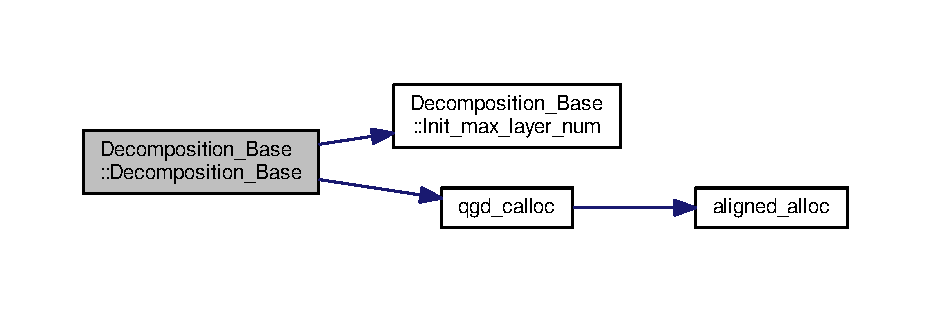
\includegraphics[width=350pt]{class_decomposition___base_a1f3d192d35a7154ac02e2bb3de80cd45_cgraph}
\end{center}
\end{figure}


\index{Decomposition\+\_\+\+Base@{Decomposition\+\_\+\+Base}!````~Decomposition\+\_\+\+Base@{$\sim$\+Decomposition\+\_\+\+Base}}
\index{````~Decomposition\+\_\+\+Base@{$\sim$\+Decomposition\+\_\+\+Base}!Decomposition\+\_\+\+Base@{Decomposition\+\_\+\+Base}}
\subsubsection[{\texorpdfstring{$\sim$\+Decomposition\+\_\+\+Base()}{~Decomposition_Base()}}]{\setlength{\rightskip}{0pt plus 5cm}Decomposition\+\_\+\+Base\+::$\sim$\+Decomposition\+\_\+\+Base (
\begin{DoxyParamCaption}
{}
\end{DoxyParamCaption}
)}\hypertarget{class_decomposition___base_ae0c67b0a277454c77e0b50e3dfd0ee84}{}\label{class_decomposition___base_ae0c67b0a277454c77e0b50e3dfd0ee84}


Destructor of the class. 



Definition at line 97 of file Decomposition\+\_\+\+Base.\+cpp.



Here is the call graph for this function\+:
\nopagebreak
\begin{figure}[H]
\begin{center}
\leavevmode
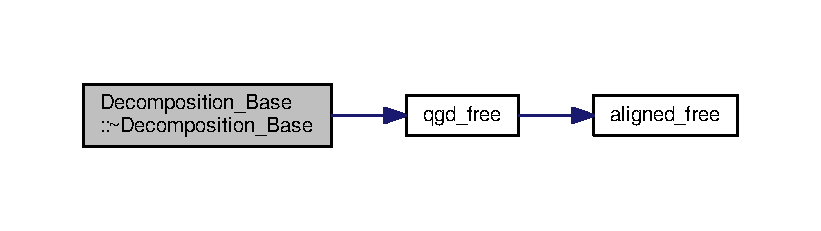
\includegraphics[width=350pt]{class_decomposition___base_ae0c67b0a277454c77e0b50e3dfd0ee84_cgraph}
\end{center}
\end{figure}


\index{Decomposition\+\_\+\+Base@{Decomposition\+\_\+\+Base}!Decomposition\+\_\+\+Base@{Decomposition\+\_\+\+Base}}
\index{Decomposition\+\_\+\+Base@{Decomposition\+\_\+\+Base}!Decomposition\+\_\+\+Base@{Decomposition\+\_\+\+Base}}
\subsubsection[{\texorpdfstring{Decomposition\+\_\+\+Base(\+Q\+G\+D\+\_\+\+Complex16 $\ast$\+Umtx\+\_\+in, int qbit\+\_\+num\+\_\+in, guess\+\_\+type initial\+\_\+guess\+\_\+in)}{Decomposition_Base(QGD_Complex16 *Umtx_in, int qbit_num_in, guess_type initial_guess_in)}}]{\setlength{\rightskip}{0pt plus 5cm}Decomposition\+\_\+\+Base\+::\+Decomposition\+\_\+\+Base (
\begin{DoxyParamCaption}
\item[{{\bf Q\+G\+D\+\_\+\+Complex16} $\ast$}]{Umtx\+\_\+in, }
\item[{int}]{qbit\+\_\+num\+\_\+in, }
\item[{{\bf guess\+\_\+type}}]{initial\+\_\+guess\+\_\+in}
\end{DoxyParamCaption}
)}\hypertarget{class_decomposition___base_a1f3d192d35a7154ac02e2bb3de80cd45}{}\label{class_decomposition___base_a1f3d192d35a7154ac02e2bb3de80cd45}


Contructor of the class. 

Constructor of the class. 
\begin{DoxyParams}{Parameters}
{\em Umtx\+\_\+in} & The unitary matrix to be decomposed \\
\hline
{\em qbit\+\_\+num\+\_\+in} & The number of qubits spanning the unitary to be decomposed. \\
\hline
{\em initial\+\_\+guess} & Type to guess the initial values for the optimalization. Possible values\+: Z\+E\+R\+OS=0, R\+A\+N\+D\+OM=1, C\+L\+O\+S\+E\+\_\+\+T\+O\+\_\+\+Z\+E\+RO=2 \\
\hline
\end{DoxyParams}
\begin{DoxyReturn}{Returns}
An instance of the class 
\end{DoxyReturn}
\index{Decomposition\+\_\+\+Base@{Decomposition\+\_\+\+Base}!````~Decomposition\+\_\+\+Base@{$\sim$\+Decomposition\+\_\+\+Base}}
\index{````~Decomposition\+\_\+\+Base@{$\sim$\+Decomposition\+\_\+\+Base}!Decomposition\+\_\+\+Base@{Decomposition\+\_\+\+Base}}
\subsubsection[{\texorpdfstring{$\sim$\+Decomposition\+\_\+\+Base()}{~Decomposition_Base()}}]{\setlength{\rightskip}{0pt plus 5cm}Decomposition\+\_\+\+Base\+::$\sim$\+Decomposition\+\_\+\+Base (
\begin{DoxyParamCaption}
{}
\end{DoxyParamCaption}
)}\hypertarget{class_decomposition___base_ae0c67b0a277454c77e0b50e3dfd0ee84}{}\label{class_decomposition___base_ae0c67b0a277454c77e0b50e3dfd0ee84}


Destructor of the class. 



\subsection{Member Function Documentation}
\index{Decomposition\+\_\+\+Base@{Decomposition\+\_\+\+Base}!add\+\_\+cnot\+\_\+to\+\_\+end@{add\+\_\+cnot\+\_\+to\+\_\+end}}
\index{add\+\_\+cnot\+\_\+to\+\_\+end@{add\+\_\+cnot\+\_\+to\+\_\+end}!Decomposition\+\_\+\+Base@{Decomposition\+\_\+\+Base}}
\subsubsection[{\texorpdfstring{add\+\_\+cnot\+\_\+to\+\_\+end(int control\+\_\+qbit, int target\+\_\+qbit)}{add_cnot_to_end(int control_qbit, int target_qbit)}}]{\setlength{\rightskip}{0pt plus 5cm}void Operation\+\_\+block\+::add\+\_\+cnot\+\_\+to\+\_\+end (
\begin{DoxyParamCaption}
\item[{int}]{control\+\_\+qbit, }
\item[{int}]{target\+\_\+qbit}
\end{DoxyParamCaption}
)\hspace{0.3cm}{\ttfamily [inherited]}}\hypertarget{class_operation__block_a3779e559654f12c5544129c46305b6ce}{}\label{class_operation__block_a3779e559654f12c5544129c46305b6ce}


Append a C\+\_\+\+N\+OT gate operation to the list of operations. 


\begin{DoxyParams}{Parameters}
{\em control\+\_\+qbit} & The identification number of the control qubit. (0 $<$= target\+\_\+qbit $<$= qbit\+\_\+num-\/1) \\
\hline
{\em target\+\_\+qbit} & The identification number of the target qubit. (0 $<$= target\+\_\+qbit $<$= qbit\+\_\+num-\/1) \\
\hline
\end{DoxyParams}


Definition at line 304 of file Operation\+\_\+block.\+cpp.



Here is the call graph for this function\+:
\nopagebreak
\begin{figure}[H]
\begin{center}
\leavevmode
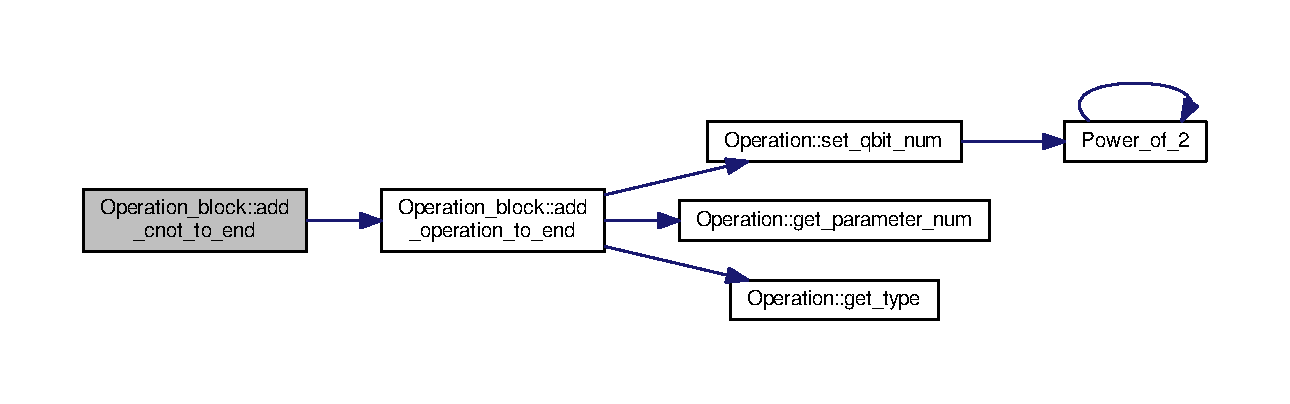
\includegraphics[width=350pt]{class_operation__block_a3779e559654f12c5544129c46305b6ce_cgraph}
\end{center}
\end{figure}




Here is the caller graph for this function\+:
\nopagebreak
\begin{figure}[H]
\begin{center}
\leavevmode
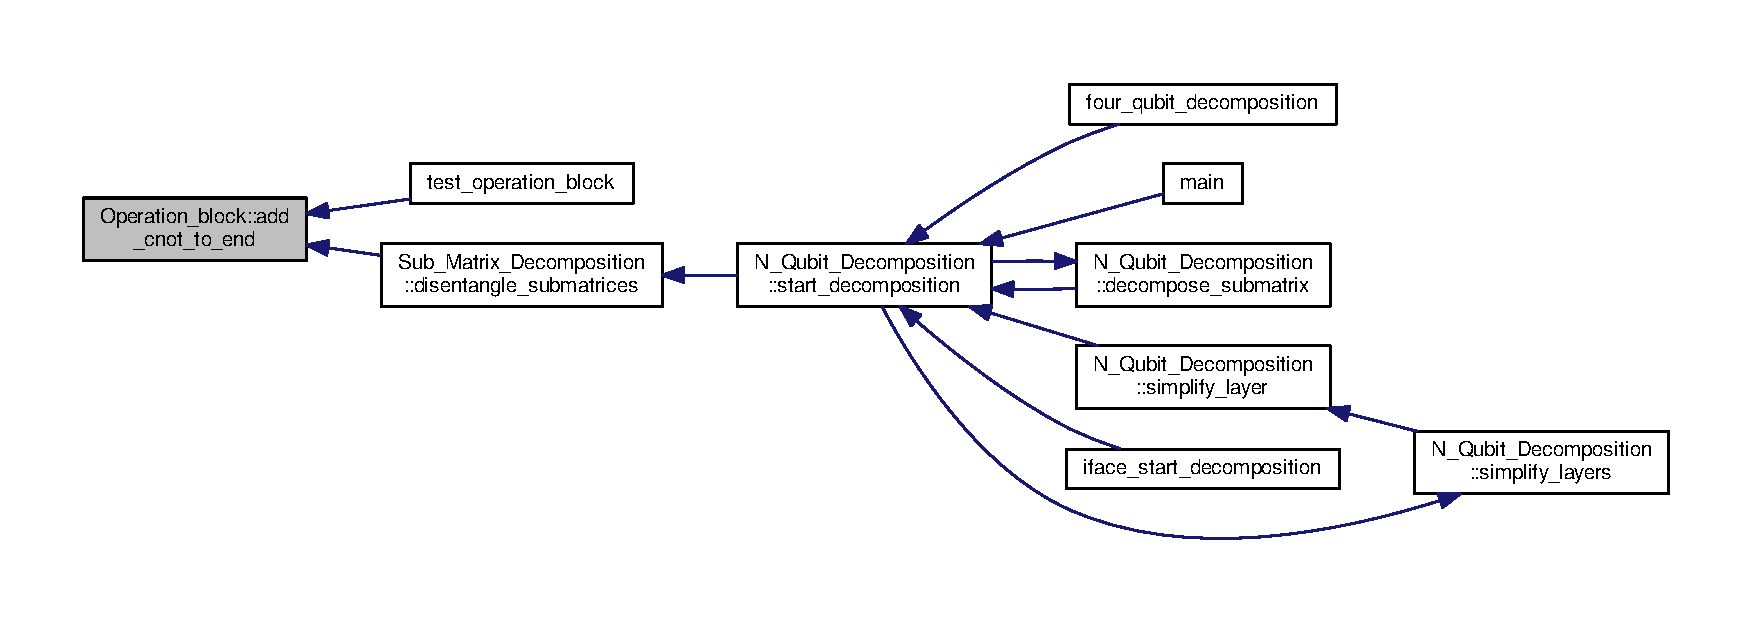
\includegraphics[width=350pt]{class_operation__block_a3779e559654f12c5544129c46305b6ce_icgraph}
\end{center}
\end{figure}


\index{Decomposition\+\_\+\+Base@{Decomposition\+\_\+\+Base}!add\+\_\+cnot\+\_\+to\+\_\+end@{add\+\_\+cnot\+\_\+to\+\_\+end}}
\index{add\+\_\+cnot\+\_\+to\+\_\+end@{add\+\_\+cnot\+\_\+to\+\_\+end}!Decomposition\+\_\+\+Base@{Decomposition\+\_\+\+Base}}
\subsubsection[{\texorpdfstring{add\+\_\+cnot\+\_\+to\+\_\+end(int control\+\_\+qbit, int target\+\_\+qbit)}{add_cnot_to_end(int control_qbit, int target_qbit)}}]{\setlength{\rightskip}{0pt plus 5cm}void Operation\+\_\+block\+::add\+\_\+cnot\+\_\+to\+\_\+end (
\begin{DoxyParamCaption}
\item[{int}]{control\+\_\+qbit, }
\item[{int}]{target\+\_\+qbit}
\end{DoxyParamCaption}
)\hspace{0.3cm}{\ttfamily [inherited]}}\hypertarget{class_operation__block_a3779e559654f12c5544129c46305b6ce}{}\label{class_operation__block_a3779e559654f12c5544129c46305b6ce}


Append a C\+\_\+\+N\+OT gate operation to the list of operations. 


\begin{DoxyParams}{Parameters}
{\em control\+\_\+qbit} & The identification number of the control qubit. (0 $<$= target\+\_\+qbit $<$= qbit\+\_\+num-\/1) \\
\hline
{\em target\+\_\+qbit} & The identification number of the target qubit. (0 $<$= target\+\_\+qbit $<$= qbit\+\_\+num-\/1) \\
\hline
\end{DoxyParams}
\index{Decomposition\+\_\+\+Base@{Decomposition\+\_\+\+Base}!add\+\_\+cnot\+\_\+to\+\_\+front@{add\+\_\+cnot\+\_\+to\+\_\+front}}
\index{add\+\_\+cnot\+\_\+to\+\_\+front@{add\+\_\+cnot\+\_\+to\+\_\+front}!Decomposition\+\_\+\+Base@{Decomposition\+\_\+\+Base}}
\subsubsection[{\texorpdfstring{add\+\_\+cnot\+\_\+to\+\_\+front(int control\+\_\+qbit, int target\+\_\+qbit)}{add_cnot_to_front(int control_qbit, int target_qbit)}}]{\setlength{\rightskip}{0pt plus 5cm}void Operation\+\_\+block\+::add\+\_\+cnot\+\_\+to\+\_\+front (
\begin{DoxyParamCaption}
\item[{int}]{control\+\_\+qbit, }
\item[{int}]{target\+\_\+qbit}
\end{DoxyParamCaption}
)\hspace{0.3cm}{\ttfamily [inherited]}}\hypertarget{class_operation__block_a207dfeddc26d79125a58e2c282bb0987}{}\label{class_operation__block_a207dfeddc26d79125a58e2c282bb0987}


Add a C\+\_\+\+N\+OT gate operation to the front of the list of operations. 


\begin{DoxyParams}{Parameters}
{\em control\+\_\+qbit} & The identification number of the control qubit. (0 $<$= target\+\_\+qbit $<$= qbit\+\_\+num-\/1) \\
\hline
{\em target\+\_\+qbit} & The identification number of the target qubit. (0 $<$= target\+\_\+qbit $<$= qbit\+\_\+num-\/1) \\
\hline
\end{DoxyParams}


Definition at line 321 of file Operation\+\_\+block.\+cpp.



Here is the call graph for this function\+:
\nopagebreak
\begin{figure}[H]
\begin{center}
\leavevmode
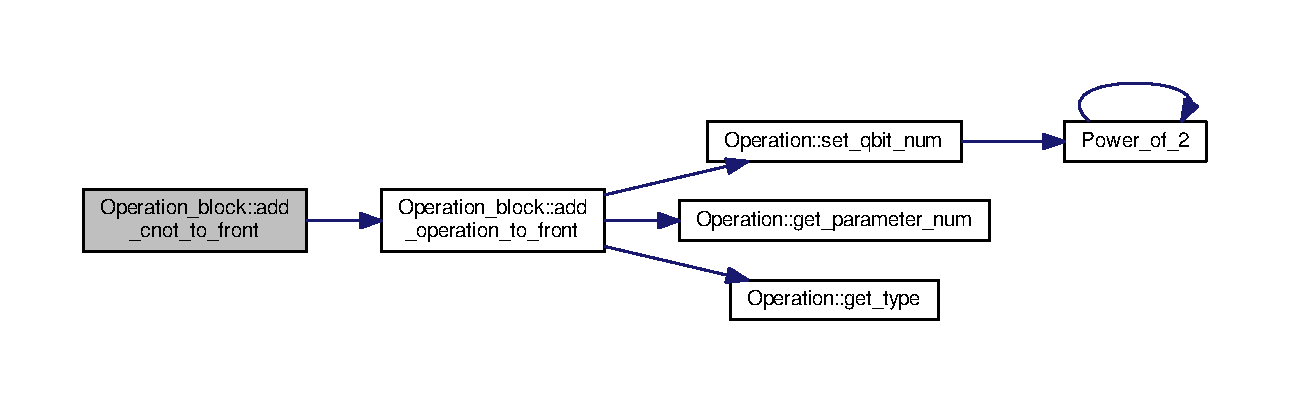
\includegraphics[width=350pt]{class_operation__block_a207dfeddc26d79125a58e2c282bb0987_cgraph}
\end{center}
\end{figure}


\index{Decomposition\+\_\+\+Base@{Decomposition\+\_\+\+Base}!add\+\_\+cnot\+\_\+to\+\_\+front@{add\+\_\+cnot\+\_\+to\+\_\+front}}
\index{add\+\_\+cnot\+\_\+to\+\_\+front@{add\+\_\+cnot\+\_\+to\+\_\+front}!Decomposition\+\_\+\+Base@{Decomposition\+\_\+\+Base}}
\subsubsection[{\texorpdfstring{add\+\_\+cnot\+\_\+to\+\_\+front(int control\+\_\+qbit, int target\+\_\+qbit)}{add_cnot_to_front(int control_qbit, int target_qbit)}}]{\setlength{\rightskip}{0pt plus 5cm}void Operation\+\_\+block\+::add\+\_\+cnot\+\_\+to\+\_\+front (
\begin{DoxyParamCaption}
\item[{int}]{control\+\_\+qbit, }
\item[{int}]{target\+\_\+qbit}
\end{DoxyParamCaption}
)\hspace{0.3cm}{\ttfamily [inherited]}}\hypertarget{class_operation__block_a207dfeddc26d79125a58e2c282bb0987}{}\label{class_operation__block_a207dfeddc26d79125a58e2c282bb0987}


Add a C\+\_\+\+N\+OT gate operation to the front of the list of operations. 


\begin{DoxyParams}{Parameters}
{\em control\+\_\+qbit} & The identification number of the control qubit. (0 $<$= target\+\_\+qbit $<$= qbit\+\_\+num-\/1) \\
\hline
{\em target\+\_\+qbit} & The identification number of the target qubit. (0 $<$= target\+\_\+qbit $<$= qbit\+\_\+num-\/1) \\
\hline
\end{DoxyParams}
\index{Decomposition\+\_\+\+Base@{Decomposition\+\_\+\+Base}!add\+\_\+operation\+\_\+to\+\_\+end@{add\+\_\+operation\+\_\+to\+\_\+end}}
\index{add\+\_\+operation\+\_\+to\+\_\+end@{add\+\_\+operation\+\_\+to\+\_\+end}!Decomposition\+\_\+\+Base@{Decomposition\+\_\+\+Base}}
\subsubsection[{\texorpdfstring{add\+\_\+operation\+\_\+to\+\_\+end(\+Operation $\ast$operation)}{add_operation_to_end(Operation *operation)}}]{\setlength{\rightskip}{0pt plus 5cm}void Operation\+\_\+block\+::add\+\_\+operation\+\_\+to\+\_\+end (
\begin{DoxyParamCaption}
\item[{{\bf Operation} $\ast$}]{operation}
\end{DoxyParamCaption}
)\hspace{0.3cm}{\ttfamily [inherited]}}\hypertarget{class_operation__block_a0048efcfca374a6b960a1092ab564f03}{}\label{class_operation__block_a0048efcfca374a6b960a1092ab564f03}


Append a general operation to the list of operations. 


\begin{DoxyParams}{Parameters}
{\em operation} & A pointer to a class \hyperlink{class_operation}{Operation} describing an operation.\\
\hline
{\em operation} & An instance of class  describing an operation. \\
\hline
\end{DoxyParams}


Definition at line 362 of file Operation\+\_\+block.\+cpp.



Here is the call graph for this function\+:
\nopagebreak
\begin{figure}[H]
\begin{center}
\leavevmode
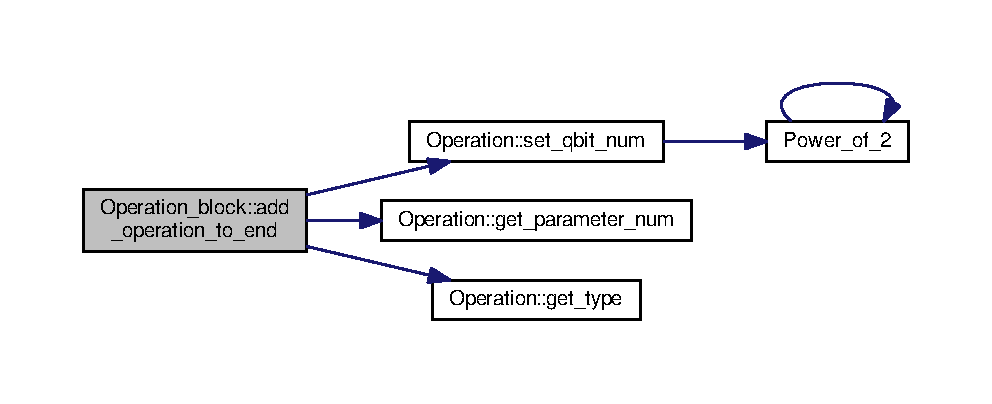
\includegraphics[width=350pt]{class_operation__block_a0048efcfca374a6b960a1092ab564f03_cgraph}
\end{center}
\end{figure}




Here is the caller graph for this function\+:
\nopagebreak
\begin{figure}[H]
\begin{center}
\leavevmode
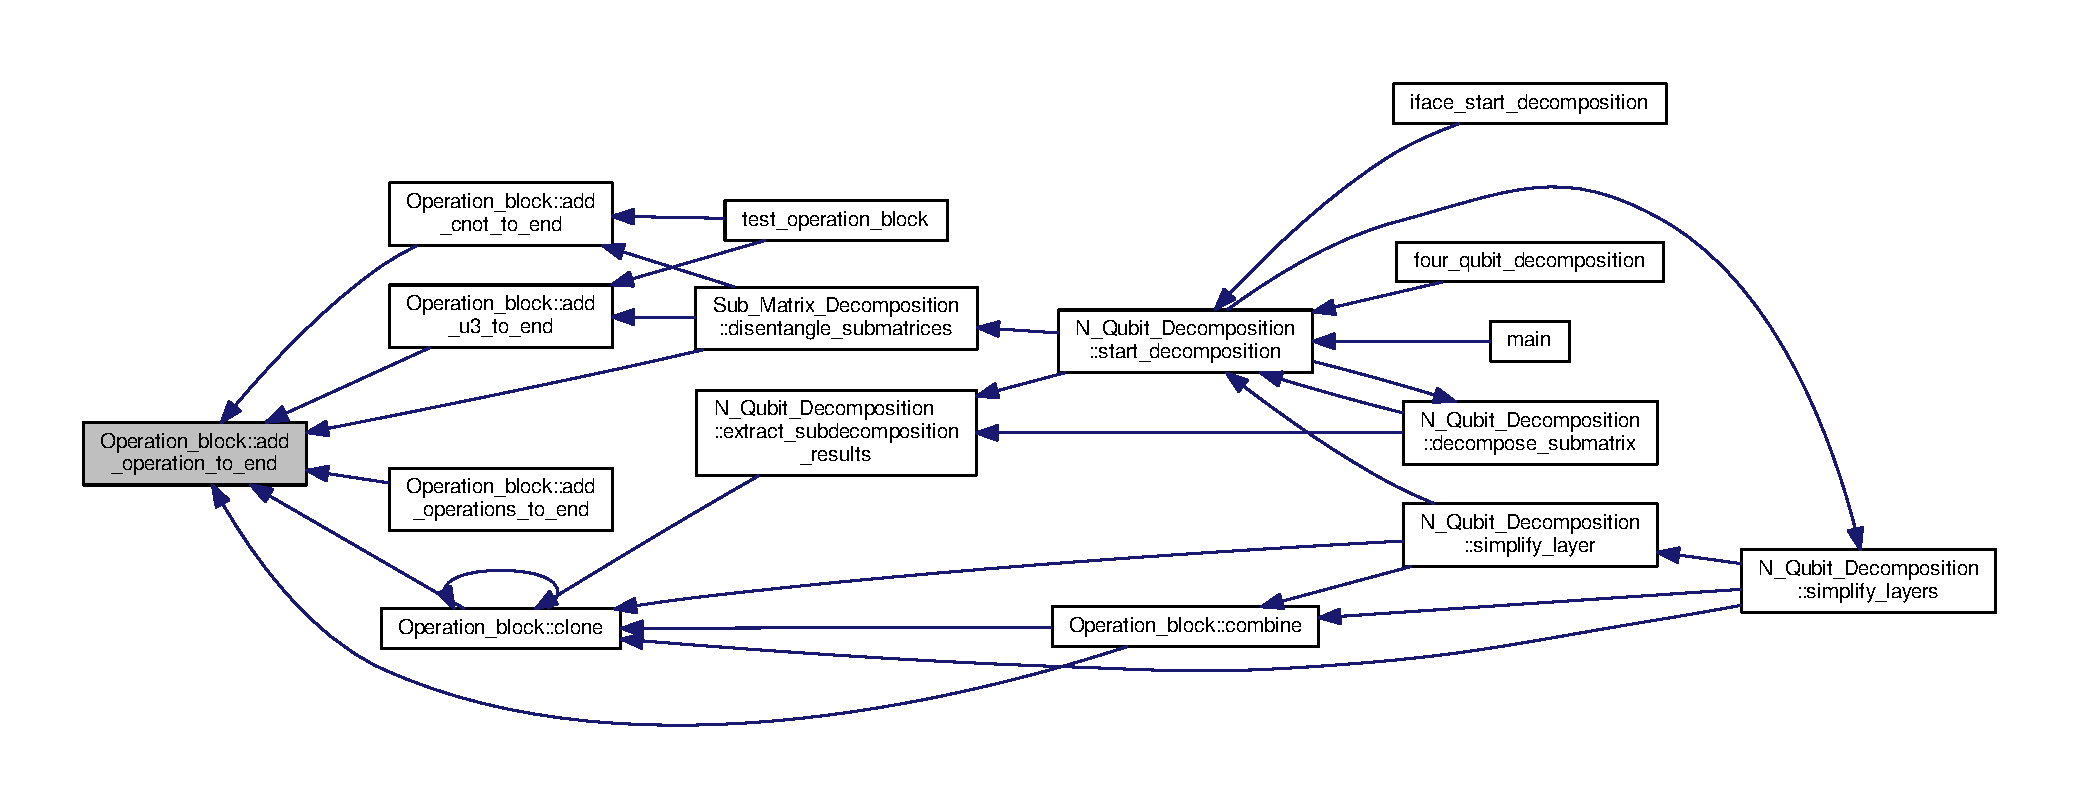
\includegraphics[width=350pt]{class_operation__block_a0048efcfca374a6b960a1092ab564f03_icgraph}
\end{center}
\end{figure}


\index{Decomposition\+\_\+\+Base@{Decomposition\+\_\+\+Base}!add\+\_\+operation\+\_\+to\+\_\+end@{add\+\_\+operation\+\_\+to\+\_\+end}}
\index{add\+\_\+operation\+\_\+to\+\_\+end@{add\+\_\+operation\+\_\+to\+\_\+end}!Decomposition\+\_\+\+Base@{Decomposition\+\_\+\+Base}}
\subsubsection[{\texorpdfstring{add\+\_\+operation\+\_\+to\+\_\+end(\+Operation $\ast$operation)}{add_operation_to_end(Operation *operation)}}]{\setlength{\rightskip}{0pt plus 5cm}void Operation\+\_\+block\+::add\+\_\+operation\+\_\+to\+\_\+end (
\begin{DoxyParamCaption}
\item[{{\bf Operation} $\ast$}]{operation}
\end{DoxyParamCaption}
)\hspace{0.3cm}{\ttfamily [inherited]}}\hypertarget{class_operation__block_a0048efcfca374a6b960a1092ab564f03}{}\label{class_operation__block_a0048efcfca374a6b960a1092ab564f03}


Append a general operation to the list of operations. 


\begin{DoxyParams}{Parameters}
{\em operation} & A pointer to a class \hyperlink{class_operation}{Operation} describing an operation. \\
\hline
\end{DoxyParams}
\index{Decomposition\+\_\+\+Base@{Decomposition\+\_\+\+Base}!add\+\_\+operation\+\_\+to\+\_\+front@{add\+\_\+operation\+\_\+to\+\_\+front}}
\index{add\+\_\+operation\+\_\+to\+\_\+front@{add\+\_\+operation\+\_\+to\+\_\+front}!Decomposition\+\_\+\+Base@{Decomposition\+\_\+\+Base}}
\subsubsection[{\texorpdfstring{add\+\_\+operation\+\_\+to\+\_\+front(\+Operation $\ast$operation)}{add_operation_to_front(Operation *operation)}}]{\setlength{\rightskip}{0pt plus 5cm}void Operation\+\_\+block\+::add\+\_\+operation\+\_\+to\+\_\+front (
\begin{DoxyParamCaption}
\item[{{\bf Operation} $\ast$}]{operation}
\end{DoxyParamCaption}
)\hspace{0.3cm}{\ttfamily [inherited]}}\hypertarget{class_operation__block_a1db22aed1f33a97bcaa2fad8c321a243}{}\label{class_operation__block_a1db22aed1f33a97bcaa2fad8c321a243}


Add an operation to the front of the list of operations. 


\begin{DoxyParams}{Parameters}
{\em operation} & A pointer to a class \hyperlink{class_operation}{Operation} describing an operation.\\
\hline
{\em operation} & A pointer to a class  describing an operation. \\
\hline
\end{DoxyParams}


Definition at line 385 of file Operation\+\_\+block.\+cpp.



Here is the call graph for this function\+:
\nopagebreak
\begin{figure}[H]
\begin{center}
\leavevmode
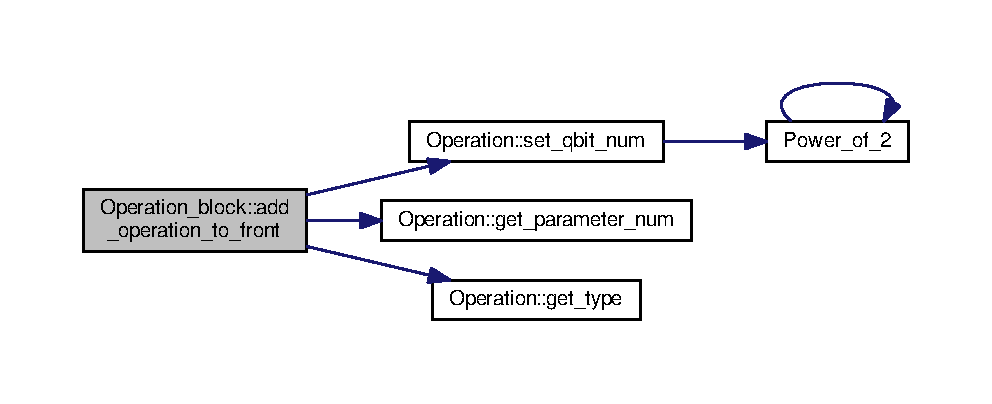
\includegraphics[width=350pt]{class_operation__block_a1db22aed1f33a97bcaa2fad8c321a243_cgraph}
\end{center}
\end{figure}




Here is the caller graph for this function\+:
\nopagebreak
\begin{figure}[H]
\begin{center}
\leavevmode
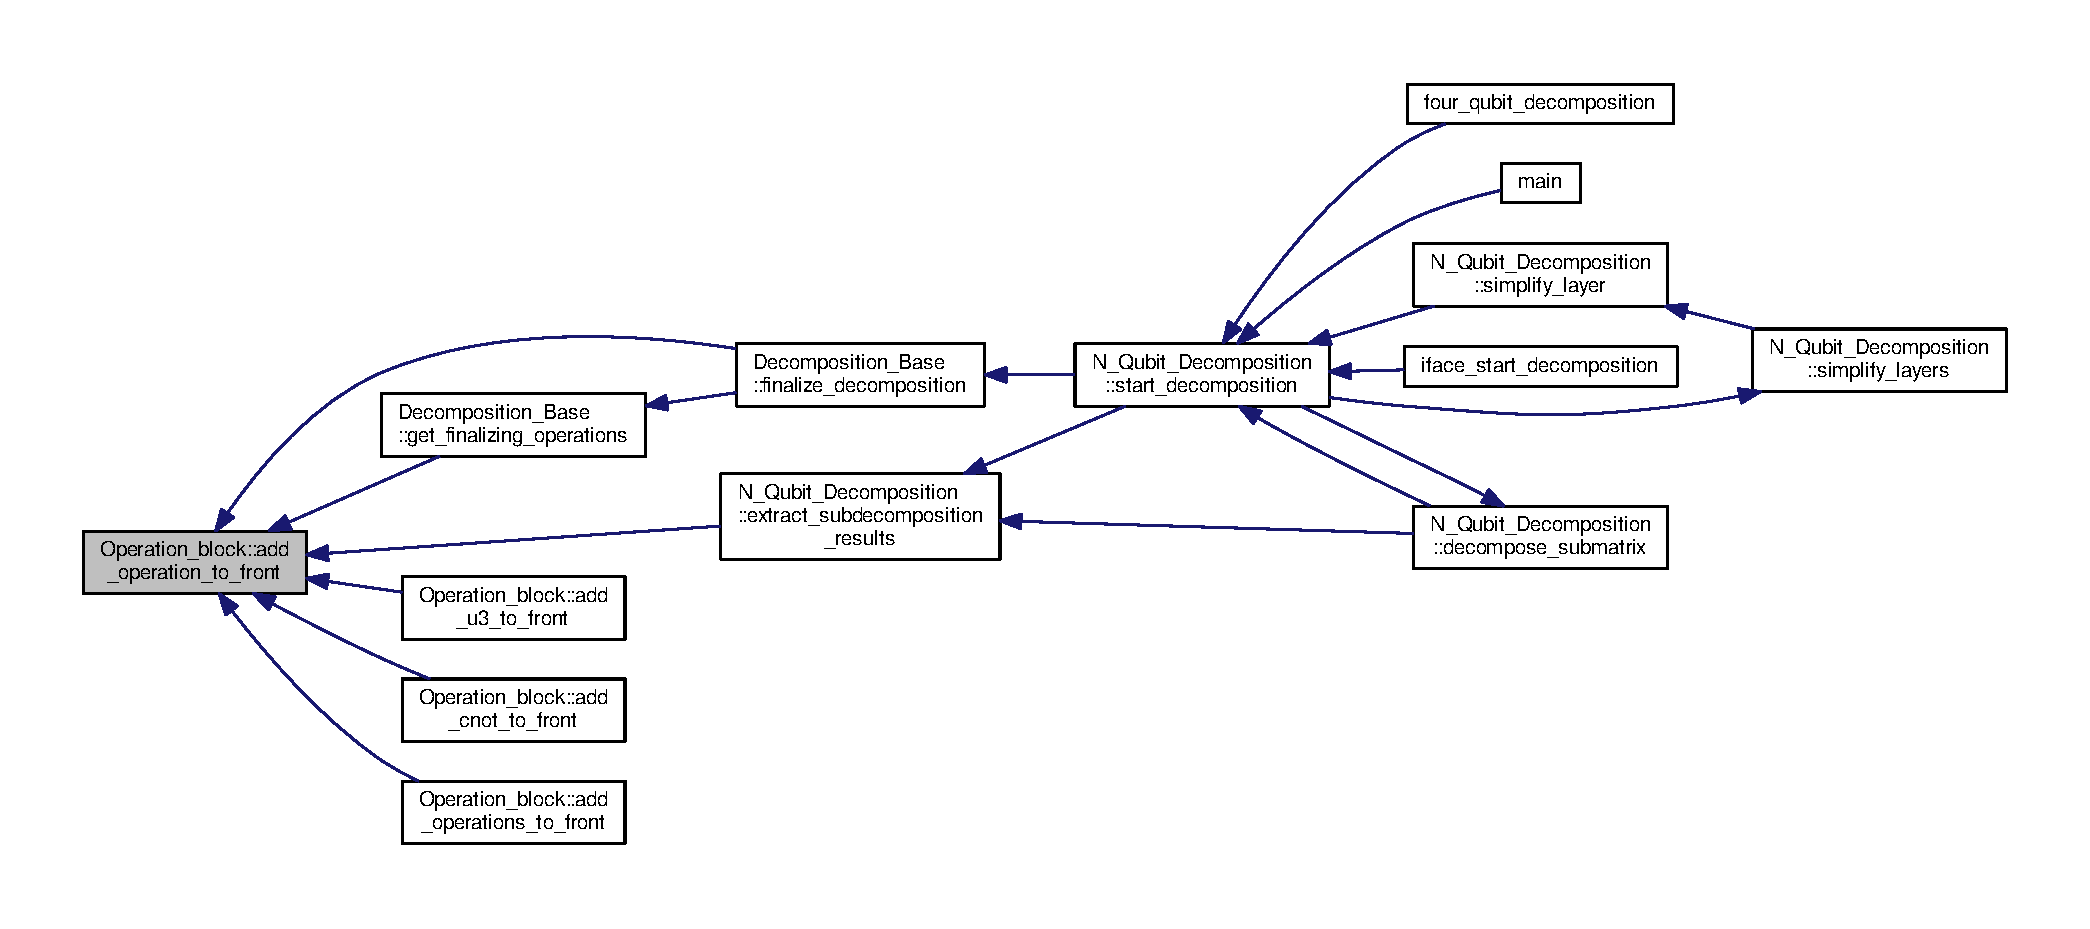
\includegraphics[width=350pt]{class_operation__block_a1db22aed1f33a97bcaa2fad8c321a243_icgraph}
\end{center}
\end{figure}


\index{Decomposition\+\_\+\+Base@{Decomposition\+\_\+\+Base}!add\+\_\+operation\+\_\+to\+\_\+front@{add\+\_\+operation\+\_\+to\+\_\+front}}
\index{add\+\_\+operation\+\_\+to\+\_\+front@{add\+\_\+operation\+\_\+to\+\_\+front}!Decomposition\+\_\+\+Base@{Decomposition\+\_\+\+Base}}
\subsubsection[{\texorpdfstring{add\+\_\+operation\+\_\+to\+\_\+front(\+Operation $\ast$operation)}{add_operation_to_front(Operation *operation)}}]{\setlength{\rightskip}{0pt plus 5cm}void Operation\+\_\+block\+::add\+\_\+operation\+\_\+to\+\_\+front (
\begin{DoxyParamCaption}
\item[{{\bf Operation} $\ast$}]{operation}
\end{DoxyParamCaption}
)\hspace{0.3cm}{\ttfamily [inherited]}}\hypertarget{class_operation__block_a1db22aed1f33a97bcaa2fad8c321a243}{}\label{class_operation__block_a1db22aed1f33a97bcaa2fad8c321a243}


Add an operation to the front of the list of operations. 


\begin{DoxyParams}{Parameters}
{\em operation} & A pointer to a class \hyperlink{class_operation}{Operation} describing an operation. \\
\hline
\end{DoxyParams}
\index{Decomposition\+\_\+\+Base@{Decomposition\+\_\+\+Base}!add\+\_\+operations\+\_\+to\+\_\+end@{add\+\_\+operations\+\_\+to\+\_\+end}}
\index{add\+\_\+operations\+\_\+to\+\_\+end@{add\+\_\+operations\+\_\+to\+\_\+end}!Decomposition\+\_\+\+Base@{Decomposition\+\_\+\+Base}}
\subsubsection[{\texorpdfstring{add\+\_\+operations\+\_\+to\+\_\+end(vector$<$ Operation $\ast$ $>$ operations\+\_\+in)}{add_operations_to_end(vector< Operation * > operations_in)}}]{\setlength{\rightskip}{0pt plus 5cm}void Operation\+\_\+block\+::add\+\_\+operations\+\_\+to\+\_\+end (
\begin{DoxyParamCaption}
\item[{vector$<$ {\bf Operation} $\ast$ $>$}]{operations\+\_\+in}
\end{DoxyParamCaption}
)\hspace{0.3cm}{\ttfamily [inherited]}}\hypertarget{class_operation__block_a2253d0a652bdce52a53d45e6d0a41abd}{}\label{class_operation__block_a2253d0a652bdce52a53d45e6d0a41abd}


Append a list of operations to the list of operations. 


\begin{DoxyParams}{Parameters}
{\em operations} & A list of operation class instances. \\
\hline
\end{DoxyParams}


Definition at line 335 of file Operation\+\_\+block.\+cpp.



Here is the call graph for this function\+:
\nopagebreak
\begin{figure}[H]
\begin{center}
\leavevmode
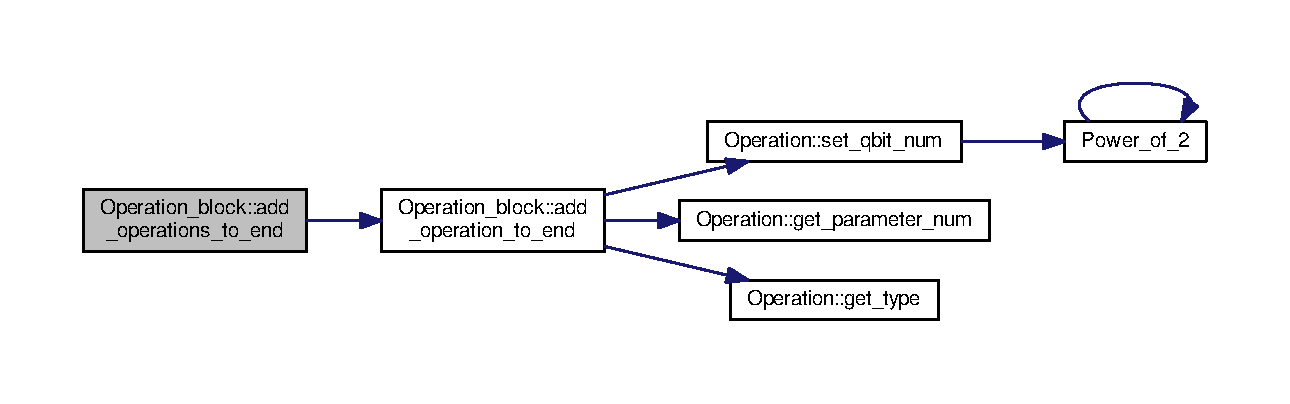
\includegraphics[width=350pt]{class_operation__block_a2253d0a652bdce52a53d45e6d0a41abd_cgraph}
\end{center}
\end{figure}


\index{Decomposition\+\_\+\+Base@{Decomposition\+\_\+\+Base}!add\+\_\+operations\+\_\+to\+\_\+end@{add\+\_\+operations\+\_\+to\+\_\+end}}
\index{add\+\_\+operations\+\_\+to\+\_\+end@{add\+\_\+operations\+\_\+to\+\_\+end}!Decomposition\+\_\+\+Base@{Decomposition\+\_\+\+Base}}
\subsubsection[{\texorpdfstring{add\+\_\+operations\+\_\+to\+\_\+end(vector$<$ Operation $\ast$ $>$ operations\+\_\+in)}{add_operations_to_end(vector< Operation * > operations_in)}}]{\setlength{\rightskip}{0pt plus 5cm}void Operation\+\_\+block\+::add\+\_\+operations\+\_\+to\+\_\+end (
\begin{DoxyParamCaption}
\item[{vector$<$ {\bf Operation} $\ast$ $>$}]{operations\+\_\+in}
\end{DoxyParamCaption}
)\hspace{0.3cm}{\ttfamily [inherited]}}\hypertarget{class_operation__block_a2253d0a652bdce52a53d45e6d0a41abd}{}\label{class_operation__block_a2253d0a652bdce52a53d45e6d0a41abd}


Append a list of operations to the list of operations. 


\begin{DoxyParams}{Parameters}
{\em operations} & A list of operation class instances. \\
\hline
\end{DoxyParams}
\index{Decomposition\+\_\+\+Base@{Decomposition\+\_\+\+Base}!add\+\_\+operations\+\_\+to\+\_\+front@{add\+\_\+operations\+\_\+to\+\_\+front}}
\index{add\+\_\+operations\+\_\+to\+\_\+front@{add\+\_\+operations\+\_\+to\+\_\+front}!Decomposition\+\_\+\+Base@{Decomposition\+\_\+\+Base}}
\subsubsection[{\texorpdfstring{add\+\_\+operations\+\_\+to\+\_\+front(vector$<$ Operation $\ast$ $>$ operations\+\_\+in)}{add_operations_to_front(vector< Operation * > operations_in)}}]{\setlength{\rightskip}{0pt plus 5cm}void Operation\+\_\+block\+::add\+\_\+operations\+\_\+to\+\_\+front (
\begin{DoxyParamCaption}
\item[{vector$<$ {\bf Operation} $\ast$ $>$}]{operations\+\_\+in}
\end{DoxyParamCaption}
)\hspace{0.3cm}{\ttfamily [inherited]}}\hypertarget{class_operation__block_a50210aa57a18243de26631e0f6f823b6}{}\label{class_operation__block_a50210aa57a18243de26631e0f6f823b6}


Add an array of operations to the front of the list of operations. 


\begin{DoxyParams}{Parameters}
{\em operations} & A list of operation class instances. \\
\hline
\end{DoxyParams}


Definition at line 348 of file Operation\+\_\+block.\+cpp.



Here is the call graph for this function\+:
\nopagebreak
\begin{figure}[H]
\begin{center}
\leavevmode
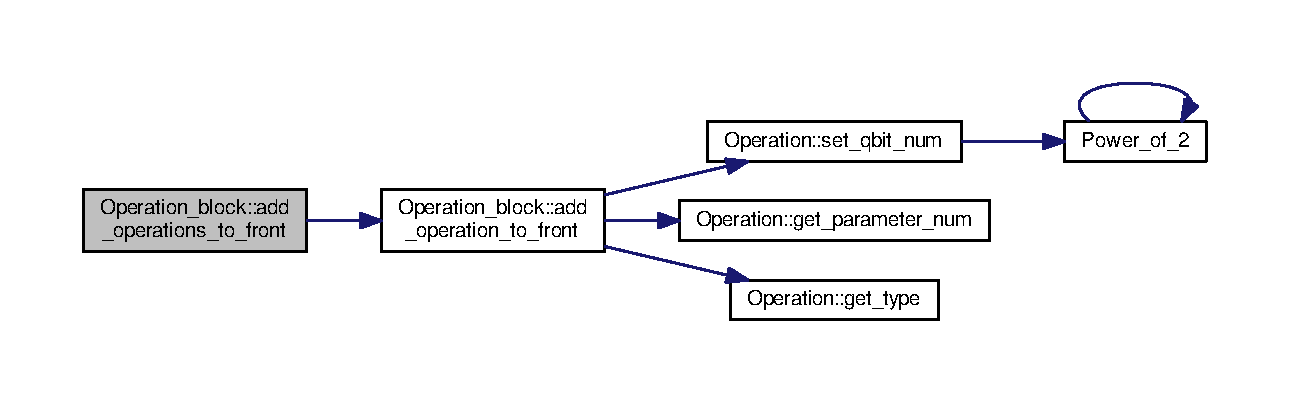
\includegraphics[width=350pt]{class_operation__block_a50210aa57a18243de26631e0f6f823b6_cgraph}
\end{center}
\end{figure}


\index{Decomposition\+\_\+\+Base@{Decomposition\+\_\+\+Base}!add\+\_\+operations\+\_\+to\+\_\+front@{add\+\_\+operations\+\_\+to\+\_\+front}}
\index{add\+\_\+operations\+\_\+to\+\_\+front@{add\+\_\+operations\+\_\+to\+\_\+front}!Decomposition\+\_\+\+Base@{Decomposition\+\_\+\+Base}}
\subsubsection[{\texorpdfstring{add\+\_\+operations\+\_\+to\+\_\+front(vector$<$ Operation $\ast$ $>$ operations\+\_\+in)}{add_operations_to_front(vector< Operation * > operations_in)}}]{\setlength{\rightskip}{0pt plus 5cm}void Operation\+\_\+block\+::add\+\_\+operations\+\_\+to\+\_\+front (
\begin{DoxyParamCaption}
\item[{vector$<$ {\bf Operation} $\ast$ $>$}]{operations\+\_\+in}
\end{DoxyParamCaption}
)\hspace{0.3cm}{\ttfamily [inherited]}}\hypertarget{class_operation__block_a50210aa57a18243de26631e0f6f823b6}{}\label{class_operation__block_a50210aa57a18243de26631e0f6f823b6}


Add an array of operations to the front of the list of operations. 


\begin{DoxyParams}{Parameters}
{\em operations} & A list of operation class instances. \\
\hline
\end{DoxyParams}
\index{Decomposition\+\_\+\+Base@{Decomposition\+\_\+\+Base}!add\+\_\+u3\+\_\+to\+\_\+end@{add\+\_\+u3\+\_\+to\+\_\+end}}
\index{add\+\_\+u3\+\_\+to\+\_\+end@{add\+\_\+u3\+\_\+to\+\_\+end}!Decomposition\+\_\+\+Base@{Decomposition\+\_\+\+Base}}
\subsubsection[{\texorpdfstring{add\+\_\+u3\+\_\+to\+\_\+end(int target\+\_\+qbit, bool Theta, bool Phi, bool Lambda)}{add_u3_to_end(int target_qbit, bool Theta, bool Phi, bool Lambda)}}]{\setlength{\rightskip}{0pt plus 5cm}void Operation\+\_\+block\+::add\+\_\+u3\+\_\+to\+\_\+end (
\begin{DoxyParamCaption}
\item[{int}]{target\+\_\+qbit, }
\item[{bool}]{Theta, }
\item[{bool}]{Phi, }
\item[{bool}]{Lambda}
\end{DoxyParamCaption}
)\hspace{0.3cm}{\ttfamily [inherited]}}\hypertarget{class_operation__block_a44940209dbc5754b676b5a493bb153f4}{}\label{class_operation__block_a44940209dbc5754b676b5a493bb153f4}


Append a \hyperlink{class_u3}{U3} gate to the list of operations. 


\begin{DoxyParams}{Parameters}
{\em target\+\_\+qbit} & The identification number of the targt qubit. (0 $<$= target\+\_\+qbit $<$= qbit\+\_\+num-\/1) \\
\hline
{\em Theta} & The Theta parameter of the \hyperlink{class_u3}{U3} operation \\
\hline
{\em Phi} & The Phi parameter of the \hyperlink{class_u3}{U3} operation \\
\hline
{\em Lambda} & The Lambda parameter of the \hyperlink{class_u3}{U3} operation \\
\hline
\end{DoxyParams}


Definition at line 273 of file Operation\+\_\+block.\+cpp.



Here is the call graph for this function\+:
\nopagebreak
\begin{figure}[H]
\begin{center}
\leavevmode
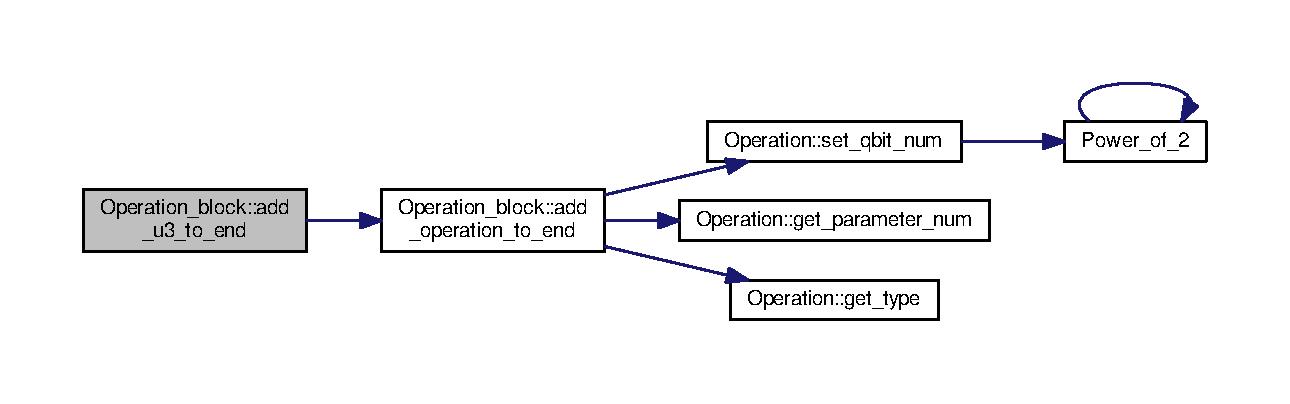
\includegraphics[width=350pt]{class_operation__block_a44940209dbc5754b676b5a493bb153f4_cgraph}
\end{center}
\end{figure}




Here is the caller graph for this function\+:
\nopagebreak
\begin{figure}[H]
\begin{center}
\leavevmode
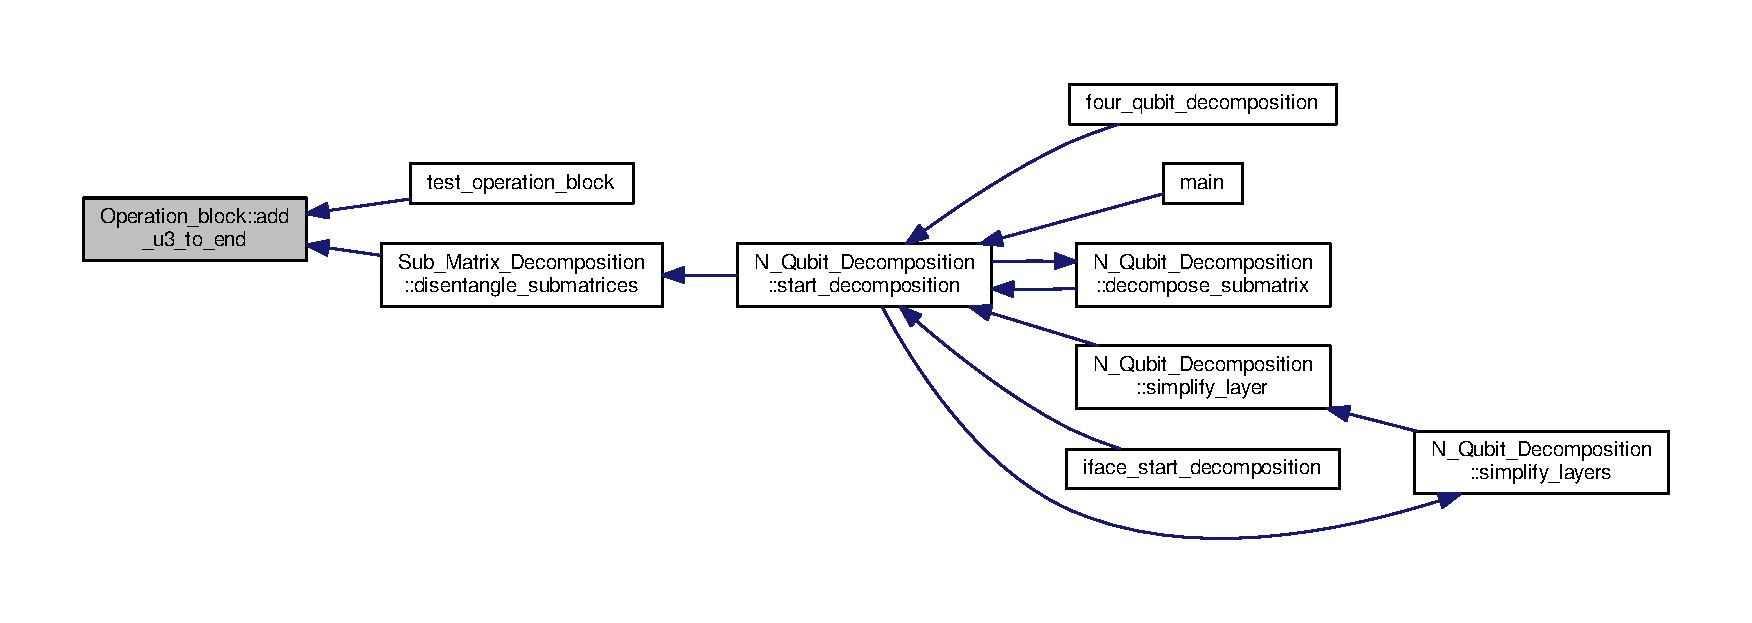
\includegraphics[width=350pt]{class_operation__block_a44940209dbc5754b676b5a493bb153f4_icgraph}
\end{center}
\end{figure}


\index{Decomposition\+\_\+\+Base@{Decomposition\+\_\+\+Base}!add\+\_\+u3\+\_\+to\+\_\+end@{add\+\_\+u3\+\_\+to\+\_\+end}}
\index{add\+\_\+u3\+\_\+to\+\_\+end@{add\+\_\+u3\+\_\+to\+\_\+end}!Decomposition\+\_\+\+Base@{Decomposition\+\_\+\+Base}}
\subsubsection[{\texorpdfstring{add\+\_\+u3\+\_\+to\+\_\+end(int target\+\_\+qbit, bool Theta, bool Phi, bool Lambda)}{add_u3_to_end(int target_qbit, bool Theta, bool Phi, bool Lambda)}}]{\setlength{\rightskip}{0pt plus 5cm}void Operation\+\_\+block\+::add\+\_\+u3\+\_\+to\+\_\+end (
\begin{DoxyParamCaption}
\item[{int}]{target\+\_\+qbit, }
\item[{bool}]{Theta, }
\item[{bool}]{Phi, }
\item[{bool}]{Lambda}
\end{DoxyParamCaption}
)\hspace{0.3cm}{\ttfamily [inherited]}}\hypertarget{class_operation__block_a44940209dbc5754b676b5a493bb153f4}{}\label{class_operation__block_a44940209dbc5754b676b5a493bb153f4}


Append a \hyperlink{class_u3}{U3} gate to the list of operations. 


\begin{DoxyParams}{Parameters}
{\em target\+\_\+qbit} & The identification number of the targt qubit. (0 $<$= target\+\_\+qbit $<$= qbit\+\_\+num-\/1) \\
\hline
{\em Theta} & The Theta parameter of the \hyperlink{class_u3}{U3} operation \\
\hline
{\em Phi} & The Phi parameter of the \hyperlink{class_u3}{U3} operation \\
\hline
{\em Lambda} & The Lambda parameter of the \hyperlink{class_u3}{U3} operation \\
\hline
\end{DoxyParams}
\index{Decomposition\+\_\+\+Base@{Decomposition\+\_\+\+Base}!add\+\_\+u3\+\_\+to\+\_\+front@{add\+\_\+u3\+\_\+to\+\_\+front}}
\index{add\+\_\+u3\+\_\+to\+\_\+front@{add\+\_\+u3\+\_\+to\+\_\+front}!Decomposition\+\_\+\+Base@{Decomposition\+\_\+\+Base}}
\subsubsection[{\texorpdfstring{add\+\_\+u3\+\_\+to\+\_\+front(int target\+\_\+qbit, bool Theta, bool Phi, bool Lambda)}{add_u3_to_front(int target_qbit, bool Theta, bool Phi, bool Lambda)}}]{\setlength{\rightskip}{0pt plus 5cm}void Operation\+\_\+block\+::add\+\_\+u3\+\_\+to\+\_\+front (
\begin{DoxyParamCaption}
\item[{int}]{target\+\_\+qbit, }
\item[{bool}]{Theta, }
\item[{bool}]{Phi, }
\item[{bool}]{Lambda}
\end{DoxyParamCaption}
)\hspace{0.3cm}{\ttfamily [inherited]}}\hypertarget{class_operation__block_ac870a2afab73fa33f706e2e35829b452}{}\label{class_operation__block_ac870a2afab73fa33f706e2e35829b452}


Add a \hyperlink{class_u3}{U3} gate to the front of the list of operations. 


\begin{DoxyParams}{Parameters}
{\em target\+\_\+qbit} & The identification number of the targt qubit. (0 $<$= target\+\_\+qbit $<$= qbit\+\_\+num-\/1) \\
\hline
{\em Theta} & The Theta parameter of the \hyperlink{class_u3}{U3} operation \\
\hline
{\em Phi} & The Phi parameter of the \hyperlink{class_u3}{U3} operation \\
\hline
{\em Lambda} & The Lambda parameter of the \hyperlink{class_u3}{U3} operation \\
\hline
\end{DoxyParams}
\index{Decomposition\+\_\+\+Base@{Decomposition\+\_\+\+Base}!add\+\_\+u3\+\_\+to\+\_\+front@{add\+\_\+u3\+\_\+to\+\_\+front}}
\index{add\+\_\+u3\+\_\+to\+\_\+front@{add\+\_\+u3\+\_\+to\+\_\+front}!Decomposition\+\_\+\+Base@{Decomposition\+\_\+\+Base}}
\subsubsection[{\texorpdfstring{add\+\_\+u3\+\_\+to\+\_\+front(int target\+\_\+qbit, bool Theta, bool Phi, bool Lambda)}{add_u3_to_front(int target_qbit, bool Theta, bool Phi, bool Lambda)}}]{\setlength{\rightskip}{0pt plus 5cm}void Operation\+\_\+block\+::add\+\_\+u3\+\_\+to\+\_\+front (
\begin{DoxyParamCaption}
\item[{int}]{target\+\_\+qbit, }
\item[{bool}]{Theta, }
\item[{bool}]{Phi, }
\item[{bool}]{Lambda}
\end{DoxyParamCaption}
)\hspace{0.3cm}{\ttfamily [inherited]}}\hypertarget{class_operation__block_ac870a2afab73fa33f706e2e35829b452}{}\label{class_operation__block_ac870a2afab73fa33f706e2e35829b452}


Add a \hyperlink{class_u3}{U3} gate to the front of the list of operations. 


\begin{DoxyParams}{Parameters}
{\em target\+\_\+qbit} & The identification number of the targt qubit. (0 $<$= target\+\_\+qbit $<$= qbit\+\_\+num-\/1) \\
\hline
{\em Theta} & The Theta parameter of the \hyperlink{class_u3}{U3} operation \\
\hline
{\em Phi} & The Phi parameter of the \hyperlink{class_u3}{U3} operation \\
\hline
{\em Lambda} & The Lambda parameter of the \hyperlink{class_u3}{U3} operation \\
\hline
\end{DoxyParams}


Definition at line 289 of file Operation\+\_\+block.\+cpp.



Here is the call graph for this function\+:
\nopagebreak
\begin{figure}[H]
\begin{center}
\leavevmode
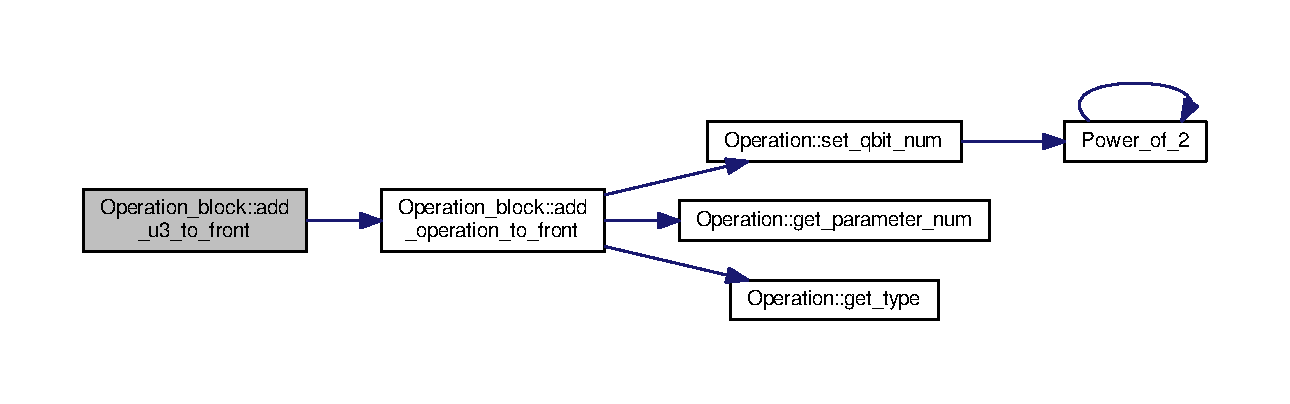
\includegraphics[width=350pt]{class_operation__block_ac870a2afab73fa33f706e2e35829b452_cgraph}
\end{center}
\end{figure}


\index{Decomposition\+\_\+\+Base@{Decomposition\+\_\+\+Base}!apply\+\_\+operation@{apply\+\_\+operation}}
\index{apply\+\_\+operation@{apply\+\_\+operation}!Decomposition\+\_\+\+Base@{Decomposition\+\_\+\+Base}}
\subsubsection[{\texorpdfstring{apply\+\_\+operation(\+Q\+G\+D\+\_\+\+Complex16 $\ast$operation\+\_\+mtx, Q\+G\+D\+\_\+\+Complex16 $\ast$input\+\_\+matrix)}{apply_operation(QGD_Complex16 *operation_mtx, QGD_Complex16 *input_matrix)}}]{\setlength{\rightskip}{0pt plus 5cm}{\bf Q\+G\+D\+\_\+\+Complex16}$\ast$ Decomposition\+\_\+\+Base\+::apply\+\_\+operation (
\begin{DoxyParamCaption}
\item[{{\bf Q\+G\+D\+\_\+\+Complex16} $\ast$}]{operation\+\_\+mtx, }
\item[{{\bf Q\+G\+D\+\_\+\+Complex16} $\ast$}]{input\+\_\+matrix}
\end{DoxyParamCaption}
)}\hypertarget{class_decomposition___base_a07d2b71ccdf4925377ee18bc552bb257}{}\label{class_decomposition___base_a07d2b71ccdf4925377ee18bc552bb257}


Apply an operations on the input matrix. 


\begin{DoxyParams}{Parameters}
{\em operation\+\_\+mtx} & The matrix of the operation. \\
\hline
{\em input\+\_\+matrix} & The input matrix to be transformed. \\
\hline
\end{DoxyParams}
\begin{DoxyReturn}{Returns}
Returns with the transformed matrix 
\end{DoxyReturn}
\index{Decomposition\+\_\+\+Base@{Decomposition\+\_\+\+Base}!apply\+\_\+operation@{apply\+\_\+operation}}
\index{apply\+\_\+operation@{apply\+\_\+operation}!Decomposition\+\_\+\+Base@{Decomposition\+\_\+\+Base}}
\subsubsection[{\texorpdfstring{apply\+\_\+operation(\+Q\+G\+D\+\_\+\+Complex16 $\ast$operation\+\_\+mtx, Q\+G\+D\+\_\+\+Complex16 $\ast$input\+\_\+matrix)}{apply_operation(QGD_Complex16 *operation_mtx, QGD_Complex16 *input_matrix)}}]{\setlength{\rightskip}{0pt plus 5cm}{\bf Q\+G\+D\+\_\+\+Complex16} $\ast$ Decomposition\+\_\+\+Base\+::apply\+\_\+operation (
\begin{DoxyParamCaption}
\item[{{\bf Q\+G\+D\+\_\+\+Complex16} $\ast$}]{operation\+\_\+mtx, }
\item[{{\bf Q\+G\+D\+\_\+\+Complex16} $\ast$}]{input\+\_\+matrix}
\end{DoxyParamCaption}
)}\hypertarget{class_decomposition___base_a4963d3fe033c225eb19a0e6f271ef37a}{}\label{class_decomposition___base_a4963d3fe033c225eb19a0e6f271ef37a}


Apply an operations on the input matrix. 


\begin{DoxyParams}{Parameters}
{\em operation\+\_\+mtx} & The matrix of the operation. \\
\hline
{\em input\+\_\+matrix} & The input matrix to be transformed. \\
\hline
\end{DoxyParams}
\begin{DoxyReturn}{Returns}
Returns with the transformed matrix
\end{DoxyReturn}

\begin{DoxyParams}{Parameters}
{\em operation\+\_\+mtx} & The matrix of the operation. \\
\hline
{\em input\+\_\+matrix} & The input matrix to be transformed. \\
\hline
{\em The} & result is returned via this matrix \\
\hline
\end{DoxyParams}


Definition at line 840 of file Decomposition\+\_\+\+Base.\+cpp.



Here is the call graph for this function\+:
\nopagebreak
\begin{figure}[H]
\begin{center}
\leavevmode
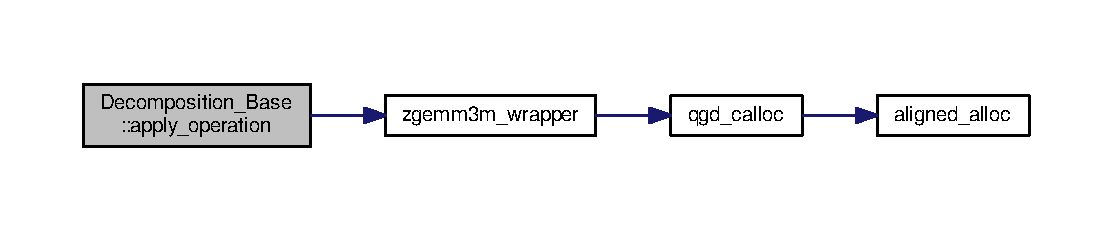
\includegraphics[width=350pt]{class_decomposition___base_a4963d3fe033c225eb19a0e6f271ef37a_cgraph}
\end{center}
\end{figure}




Here is the caller graph for this function\+:
\nopagebreak
\begin{figure}[H]
\begin{center}
\leavevmode
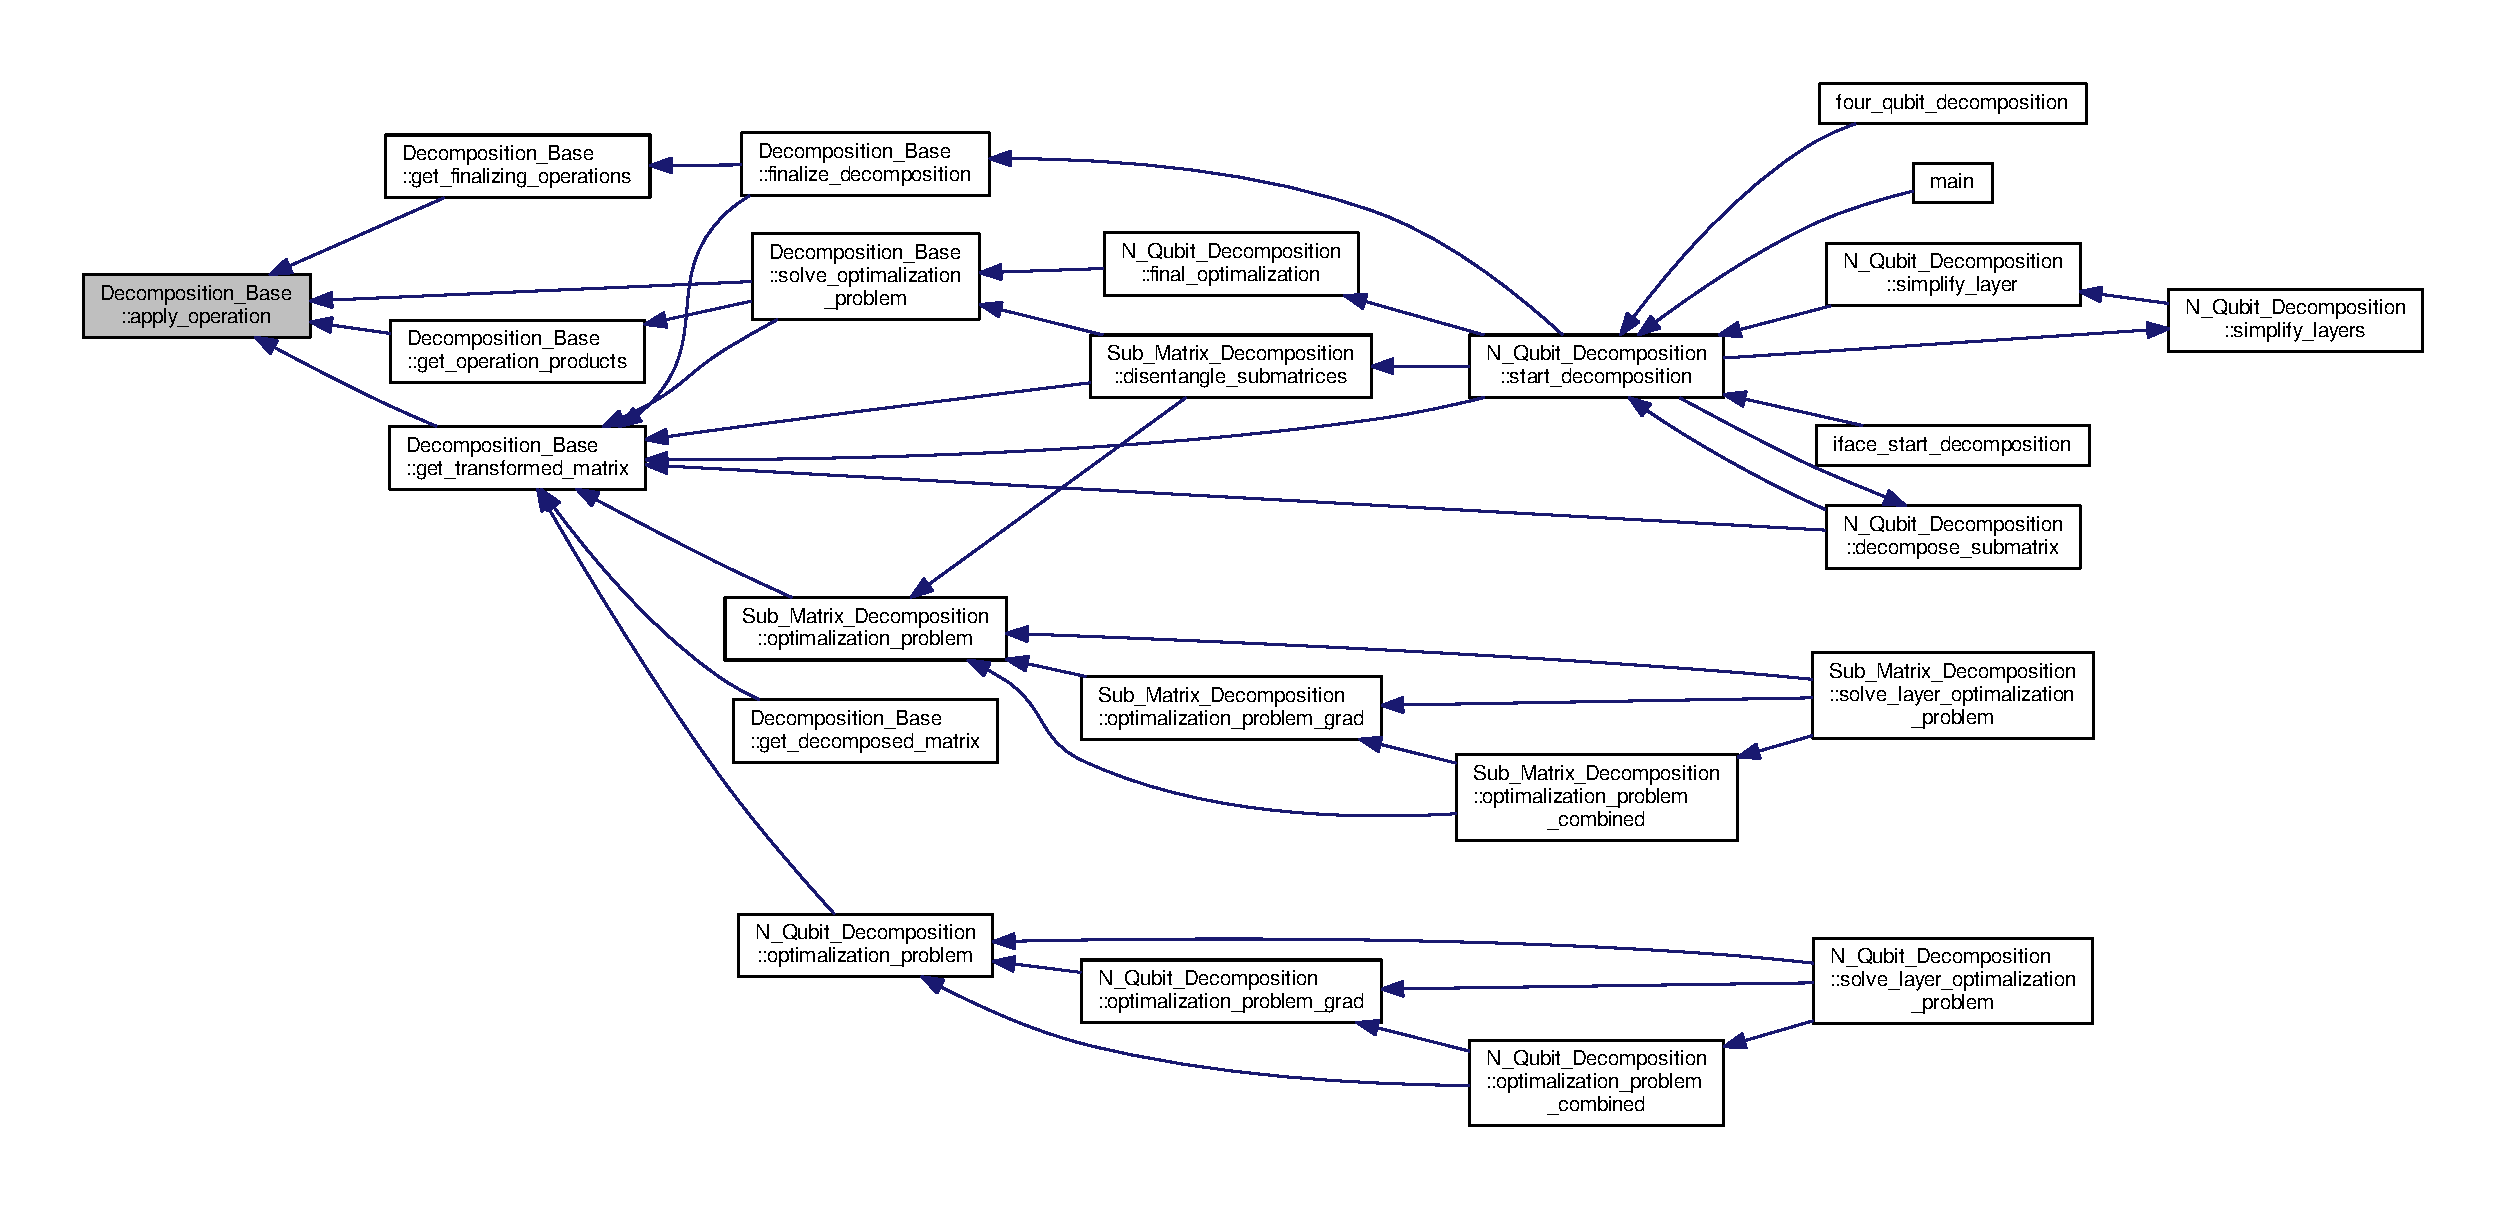
\includegraphics[width=350pt]{class_decomposition___base_a4963d3fe033c225eb19a0e6f271ef37a_icgraph}
\end{center}
\end{figure}


\index{Decomposition\+\_\+\+Base@{Decomposition\+\_\+\+Base}!apply\+\_\+operation@{apply\+\_\+operation}}
\index{apply\+\_\+operation@{apply\+\_\+operation}!Decomposition\+\_\+\+Base@{Decomposition\+\_\+\+Base}}
\subsubsection[{\texorpdfstring{apply\+\_\+operation(\+Q\+G\+D\+\_\+\+Complex16 $\ast$operation\+\_\+mtx, Q\+G\+D\+\_\+\+Complex16 $\ast$input\+\_\+matrix, Q\+G\+D\+\_\+\+Complex16 $\ast$result\+\_\+matrix)}{apply_operation(QGD_Complex16 *operation_mtx, QGD_Complex16 *input_matrix, QGD_Complex16 *result_matrix)}}]{\setlength{\rightskip}{0pt plus 5cm}int Decomposition\+\_\+\+Base\+::apply\+\_\+operation (
\begin{DoxyParamCaption}
\item[{{\bf Q\+G\+D\+\_\+\+Complex16} $\ast$}]{operation\+\_\+mtx, }
\item[{{\bf Q\+G\+D\+\_\+\+Complex16} $\ast$}]{input\+\_\+matrix, }
\item[{{\bf Q\+G\+D\+\_\+\+Complex16} $\ast$}]{result\+\_\+matrix}
\end{DoxyParamCaption}
)}\hypertarget{class_decomposition___base_aa6d12ac493c26af71613bc570fb87858}{}\label{class_decomposition___base_aa6d12ac493c26af71613bc570fb87858}


Apply an operations on the input matrix. 


\begin{DoxyParams}{Parameters}
{\em operation\+\_\+mtx} & The matrix of the operation. \\
\hline
{\em input\+\_\+matrix} & The input matrix to be transformed. \\
\hline
{\em The} & result is returned via this matrix \\
\hline
\end{DoxyParams}


Definition at line 852 of file Decomposition\+\_\+\+Base.\+cpp.



Here is the call graph for this function\+:
\nopagebreak
\begin{figure}[H]
\begin{center}
\leavevmode
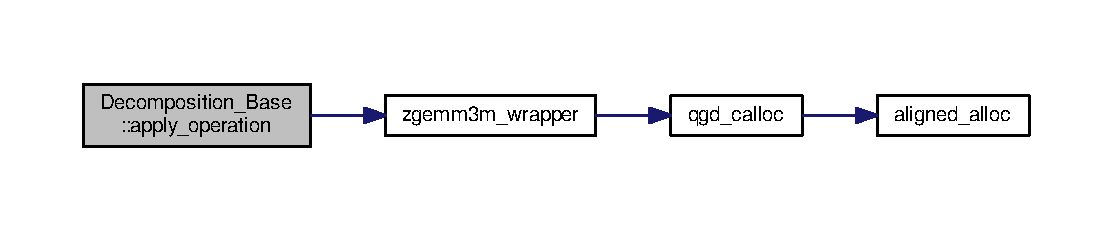
\includegraphics[width=350pt]{class_decomposition___base_aa6d12ac493c26af71613bc570fb87858_cgraph}
\end{center}
\end{figure}


\index{Decomposition\+\_\+\+Base@{Decomposition\+\_\+\+Base}!apply\+\_\+operation@{apply\+\_\+operation}}
\index{apply\+\_\+operation@{apply\+\_\+operation}!Decomposition\+\_\+\+Base@{Decomposition\+\_\+\+Base}}
\subsubsection[{\texorpdfstring{apply\+\_\+operation(\+Q\+G\+D\+\_\+\+Complex16 $\ast$operation\+\_\+mtx, Q\+G\+D\+\_\+\+Complex16 $\ast$input\+\_\+matrix, Q\+G\+D\+\_\+\+Complex16 $\ast$result\+\_\+matrix)}{apply_operation(QGD_Complex16 *operation_mtx, QGD_Complex16 *input_matrix, QGD_Complex16 *result_matrix)}}]{\setlength{\rightskip}{0pt plus 5cm}int Decomposition\+\_\+\+Base\+::apply\+\_\+operation (
\begin{DoxyParamCaption}
\item[{{\bf Q\+G\+D\+\_\+\+Complex16} $\ast$}]{operation\+\_\+mtx, }
\item[{{\bf Q\+G\+D\+\_\+\+Complex16} $\ast$}]{input\+\_\+matrix, }
\item[{{\bf Q\+G\+D\+\_\+\+Complex16} $\ast$}]{result\+\_\+matrix}
\end{DoxyParamCaption}
)}\hypertarget{class_decomposition___base_aa6d12ac493c26af71613bc570fb87858}{}\label{class_decomposition___base_aa6d12ac493c26af71613bc570fb87858}


Apply an operations on the input matrix. 


\begin{DoxyParams}{Parameters}
{\em operation\+\_\+mtx} & The matrix of the operation. \\
\hline
{\em input\+\_\+matrix} & The input matrix to be transformed. \\
\hline
{\em The} & result is returned via this matrix \\
\hline
\end{DoxyParams}
\index{Decomposition\+\_\+\+Base@{Decomposition\+\_\+\+Base}!check\+\_\+optimalization\+\_\+solution@{check\+\_\+optimalization\+\_\+solution}}
\index{check\+\_\+optimalization\+\_\+solution@{check\+\_\+optimalization\+\_\+solution}!Decomposition\+\_\+\+Base@{Decomposition\+\_\+\+Base}}
\subsubsection[{\texorpdfstring{check\+\_\+optimalization\+\_\+solution()}{check_optimalization_solution()}}]{\setlength{\rightskip}{0pt plus 5cm}bool Decomposition\+\_\+\+Base\+::check\+\_\+optimalization\+\_\+solution (
\begin{DoxyParamCaption}
{}
\end{DoxyParamCaption}
)}\hypertarget{class_decomposition___base_aa01a8d70b76215a235cb0d71894b2595}{}\label{class_decomposition___base_aa01a8d70b76215a235cb0d71894b2595}


check\+\_\+optimalization\+\_\+solution 

Checks the convergence of the optimalization problem. \begin{DoxyReturn}{Returns}
Returns with true if the target global minimum was reached during the optimalization process, or false otherwise. 
\end{DoxyReturn}
\index{Decomposition\+\_\+\+Base@{Decomposition\+\_\+\+Base}!check\+\_\+optimalization\+\_\+solution@{check\+\_\+optimalization\+\_\+solution}}
\index{check\+\_\+optimalization\+\_\+solution@{check\+\_\+optimalization\+\_\+solution}!Decomposition\+\_\+\+Base@{Decomposition\+\_\+\+Base}}
\subsubsection[{\texorpdfstring{check\+\_\+optimalization\+\_\+solution()}{check_optimalization_solution()}}]{\setlength{\rightskip}{0pt plus 5cm}bool Decomposition\+\_\+\+Base\+::check\+\_\+optimalization\+\_\+solution (
\begin{DoxyParamCaption}
{}
\end{DoxyParamCaption}
)}\hypertarget{class_decomposition___base_aa01a8d70b76215a235cb0d71894b2595}{}\label{class_decomposition___base_aa01a8d70b76215a235cb0d71894b2595}


check\+\_\+optimalization\+\_\+solution 

Checks the convergence of the optimalization problem. \begin{DoxyReturn}{Returns}
Returns with true if the target global minimum was reached during the optimalization process, or false otherwise. 
\end{DoxyReturn}


Definition at line 619 of file Decomposition\+\_\+\+Base.\+cpp.



Here is the caller graph for this function\+:
\nopagebreak
\begin{figure}[H]
\begin{center}
\leavevmode
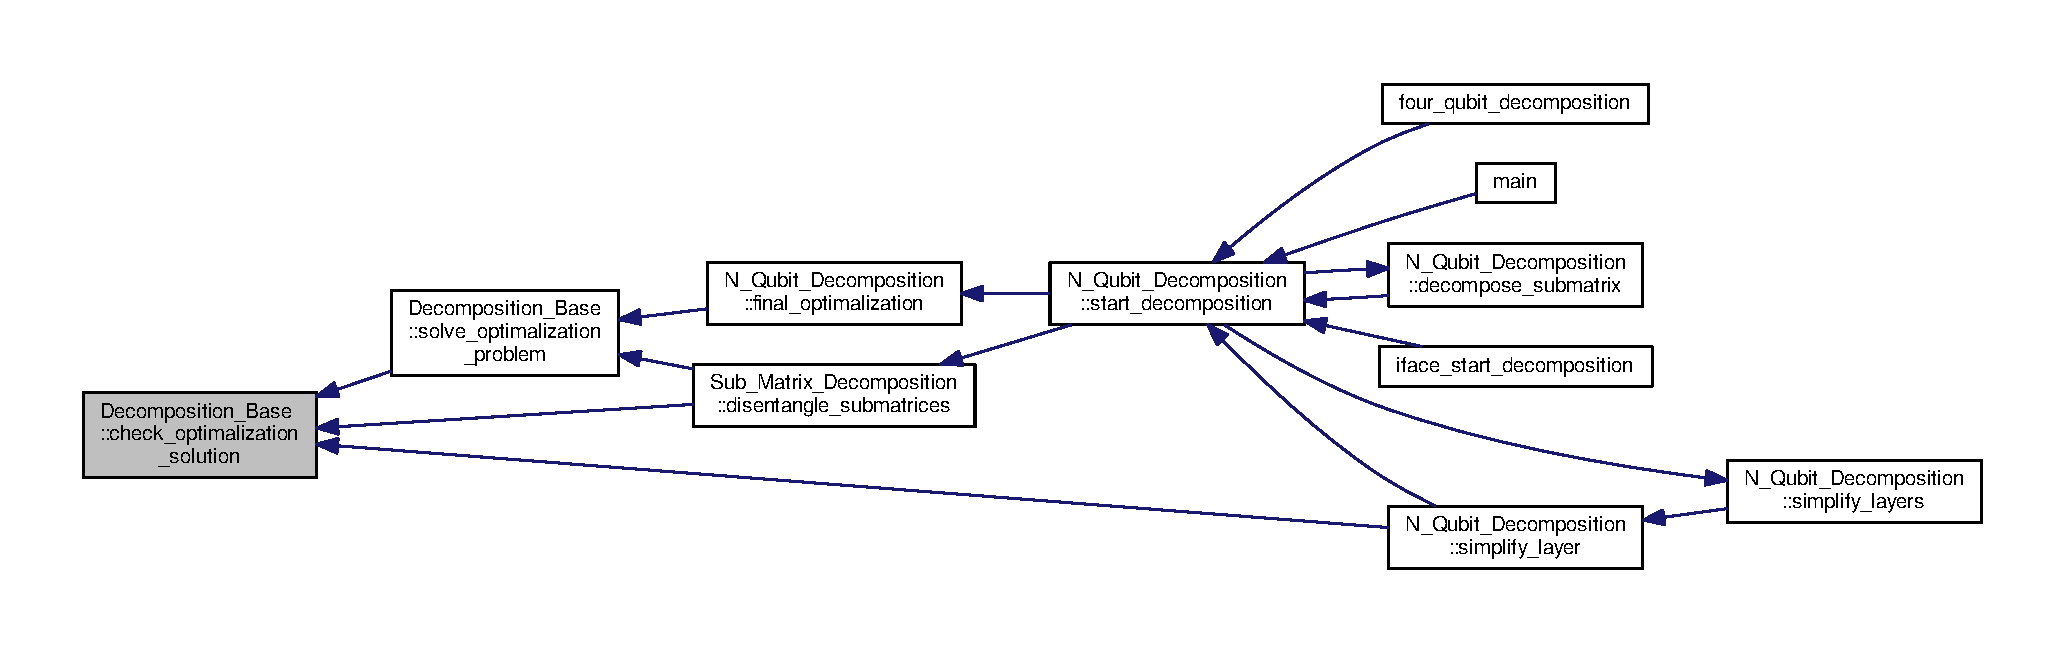
\includegraphics[width=350pt]{class_decomposition___base_aa01a8d70b76215a235cb0d71894b2595_icgraph}
\end{center}
\end{figure}


\index{Decomposition\+\_\+\+Base@{Decomposition\+\_\+\+Base}!clone@{clone}}
\index{clone@{clone}!Decomposition\+\_\+\+Base@{Decomposition\+\_\+\+Base}}
\subsubsection[{\texorpdfstring{clone()}{clone()}}]{\setlength{\rightskip}{0pt plus 5cm}{\bf Operation\+\_\+block} $\ast$ Operation\+\_\+block\+::clone (
\begin{DoxyParamCaption}
{}
\end{DoxyParamCaption}
)\hspace{0.3cm}{\ttfamily [inherited]}}\hypertarget{class_operation__block_a2aa75d20b21c3b5802730c0abe54db5e}{}\label{class_operation__block_a2aa75d20b21c3b5802730c0abe54db5e}


Create a clone of the present class. 

\begin{DoxyReturn}{Returns}
Return with a pointer pointing to the cloned object. 
\end{DoxyReturn}


Definition at line 698 of file Operation\+\_\+block.\+cpp.



Here is the call graph for this function\+:
\nopagebreak
\begin{figure}[H]
\begin{center}
\leavevmode
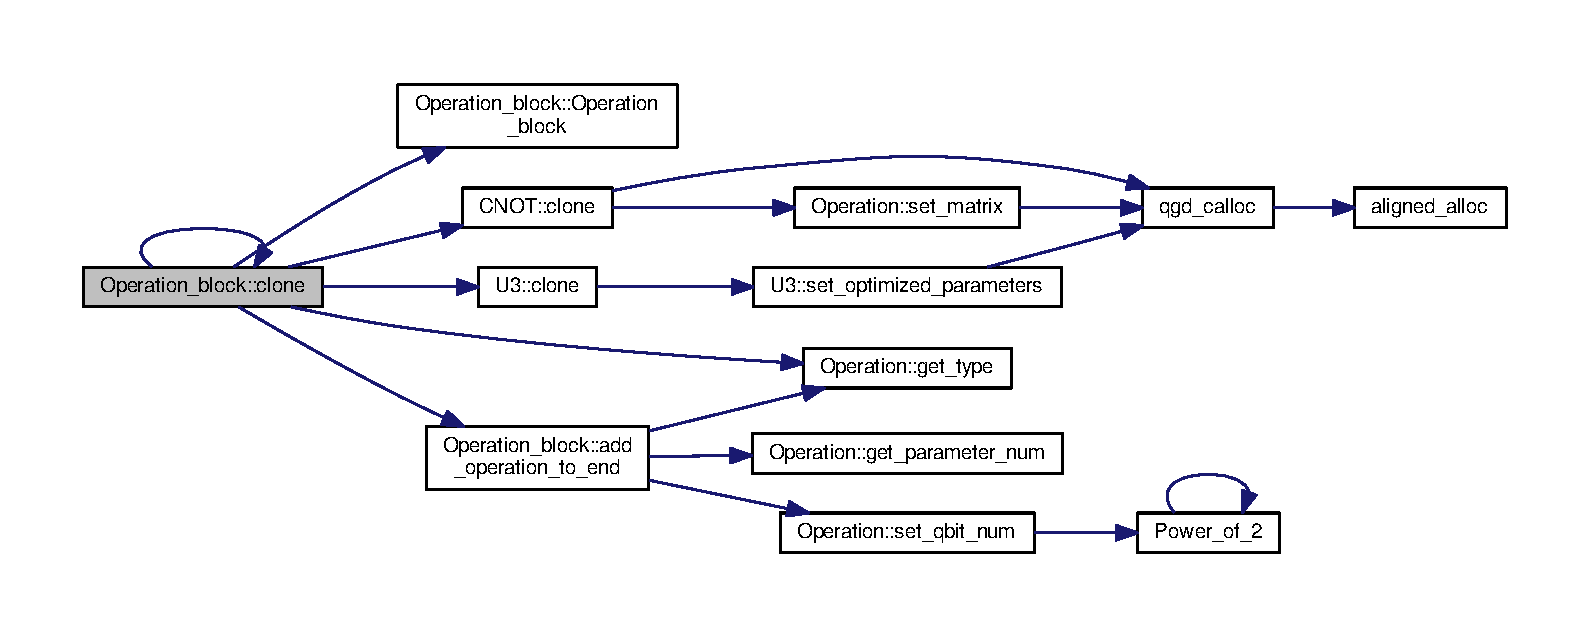
\includegraphics[width=350pt]{class_operation__block_a2aa75d20b21c3b5802730c0abe54db5e_cgraph}
\end{center}
\end{figure}




Here is the caller graph for this function\+:
\nopagebreak
\begin{figure}[H]
\begin{center}
\leavevmode
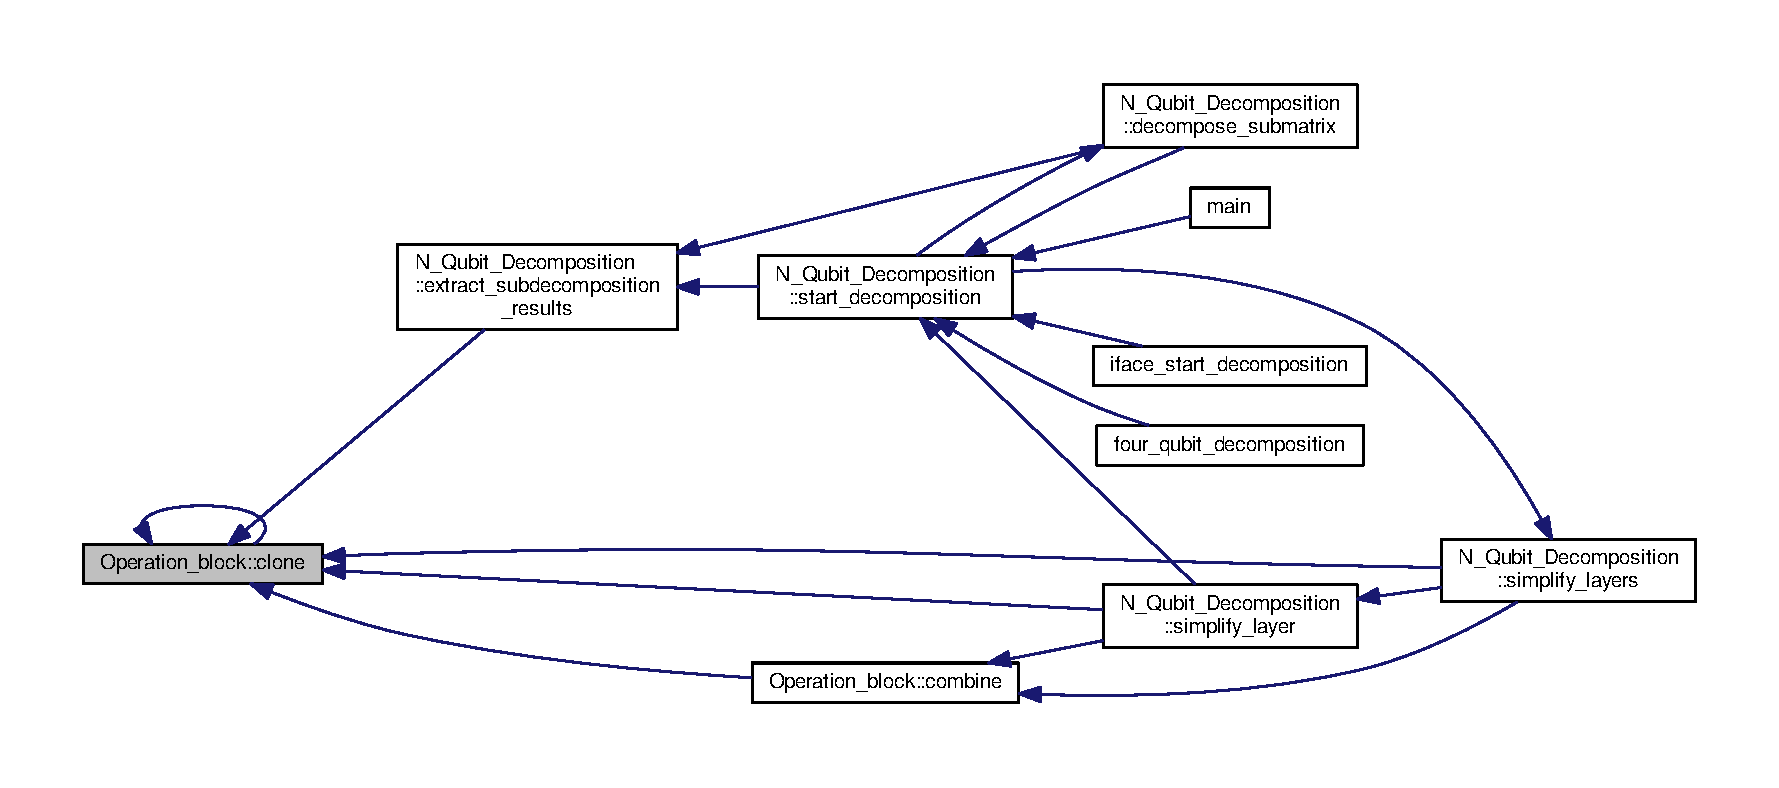
\includegraphics[width=350pt]{class_operation__block_a2aa75d20b21c3b5802730c0abe54db5e_icgraph}
\end{center}
\end{figure}


\index{Decomposition\+\_\+\+Base@{Decomposition\+\_\+\+Base}!clone@{clone}}
\index{clone@{clone}!Decomposition\+\_\+\+Base@{Decomposition\+\_\+\+Base}}
\subsubsection[{\texorpdfstring{clone()}{clone()}}]{\setlength{\rightskip}{0pt plus 5cm}{\bf Operation\+\_\+block}$\ast$ Operation\+\_\+block\+::clone (
\begin{DoxyParamCaption}
{}
\end{DoxyParamCaption}
)\hspace{0.3cm}{\ttfamily [inherited]}}\hypertarget{class_operation__block_af5d1f81be3a54eada1de293d1e9877c5}{}\label{class_operation__block_af5d1f81be3a54eada1de293d1e9877c5}


Create a clone of the present class. 

\begin{DoxyReturn}{Returns}
Return with a pointer pointing to the cloned object. 
\end{DoxyReturn}
\index{Decomposition\+\_\+\+Base@{Decomposition\+\_\+\+Base}!combine@{combine}}
\index{combine@{combine}!Decomposition\+\_\+\+Base@{Decomposition\+\_\+\+Base}}
\subsubsection[{\texorpdfstring{combine(\+Operation\+\_\+block $\ast$op\+\_\+block)}{combine(Operation_block *op_block)}}]{\setlength{\rightskip}{0pt plus 5cm}void Operation\+\_\+block\+::combine (
\begin{DoxyParamCaption}
\item[{{\bf Operation\+\_\+block} $\ast$}]{op\+\_\+block}
\end{DoxyParamCaption}
)\hspace{0.3cm}{\ttfamily [inherited]}}\hypertarget{class_operation__block_a60062cf6f48ebfdcaae9db3367a66147}{}\label{class_operation__block_a60062cf6f48ebfdcaae9db3367a66147}


Call to append the operations of an operation block to the current block. 


\begin{DoxyParams}{Parameters}
{\em op\+\_\+block} & A pointer to an instance of class \hyperlink{class_operation__block}{Operation\+\_\+block}\\
\hline
{\em op\+\_\+block} & A pointer to an instance of class  \\
\hline
\end{DoxyParams}


Definition at line 633 of file Operation\+\_\+block.\+cpp.



Here is the call graph for this function\+:
\nopagebreak
\begin{figure}[H]
\begin{center}
\leavevmode
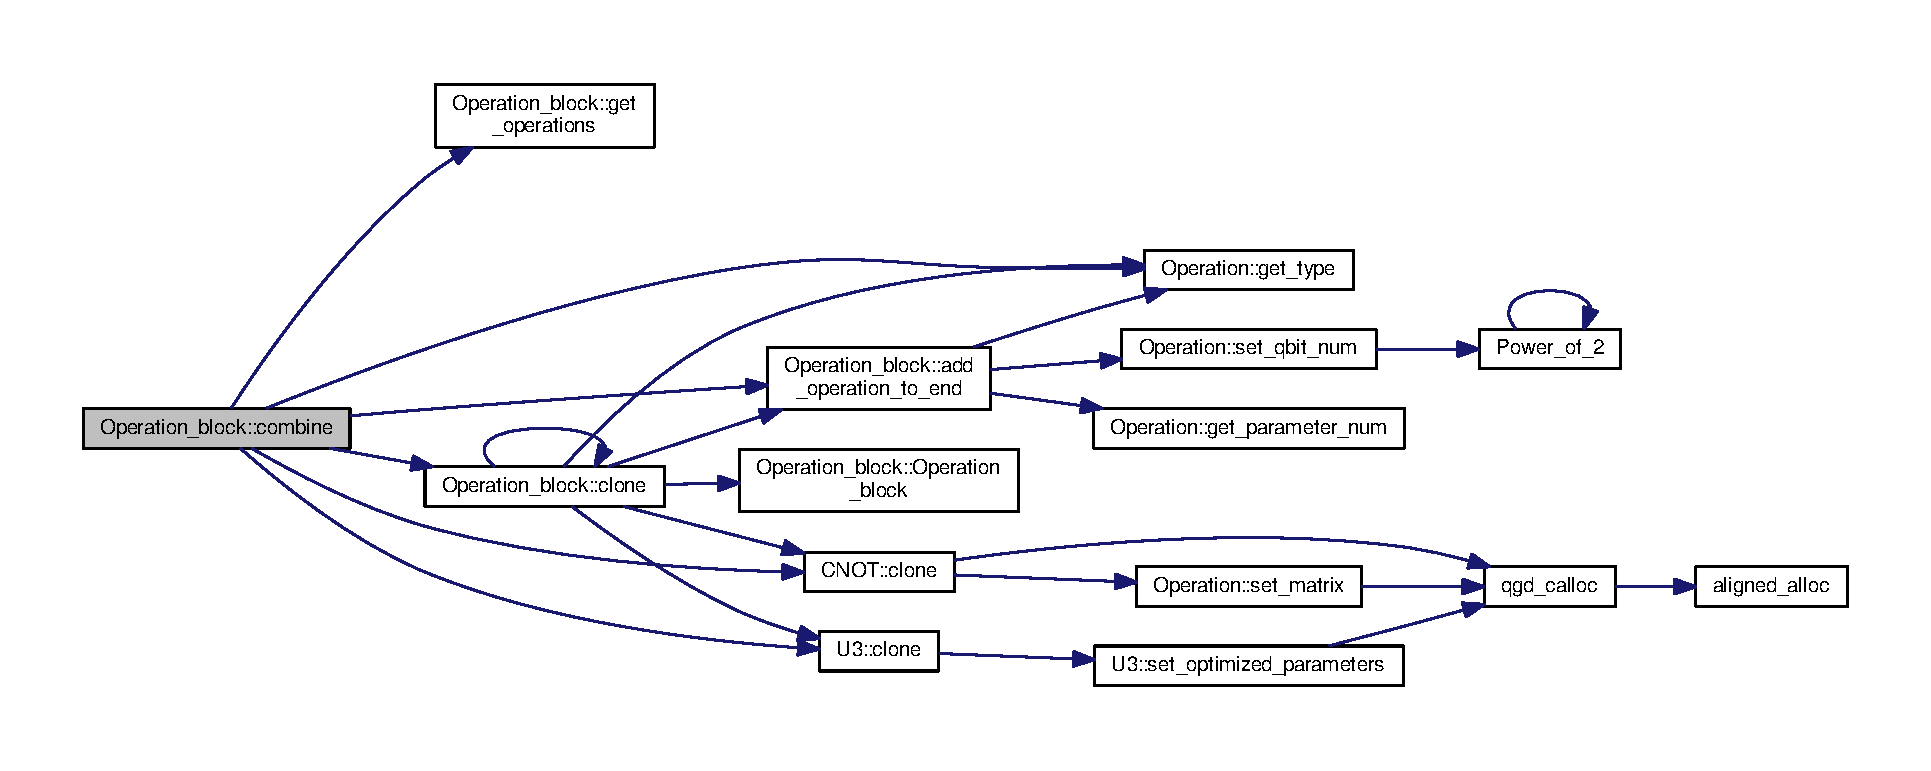
\includegraphics[width=350pt]{class_operation__block_a60062cf6f48ebfdcaae9db3367a66147_cgraph}
\end{center}
\end{figure}




Here is the caller graph for this function\+:
\nopagebreak
\begin{figure}[H]
\begin{center}
\leavevmode
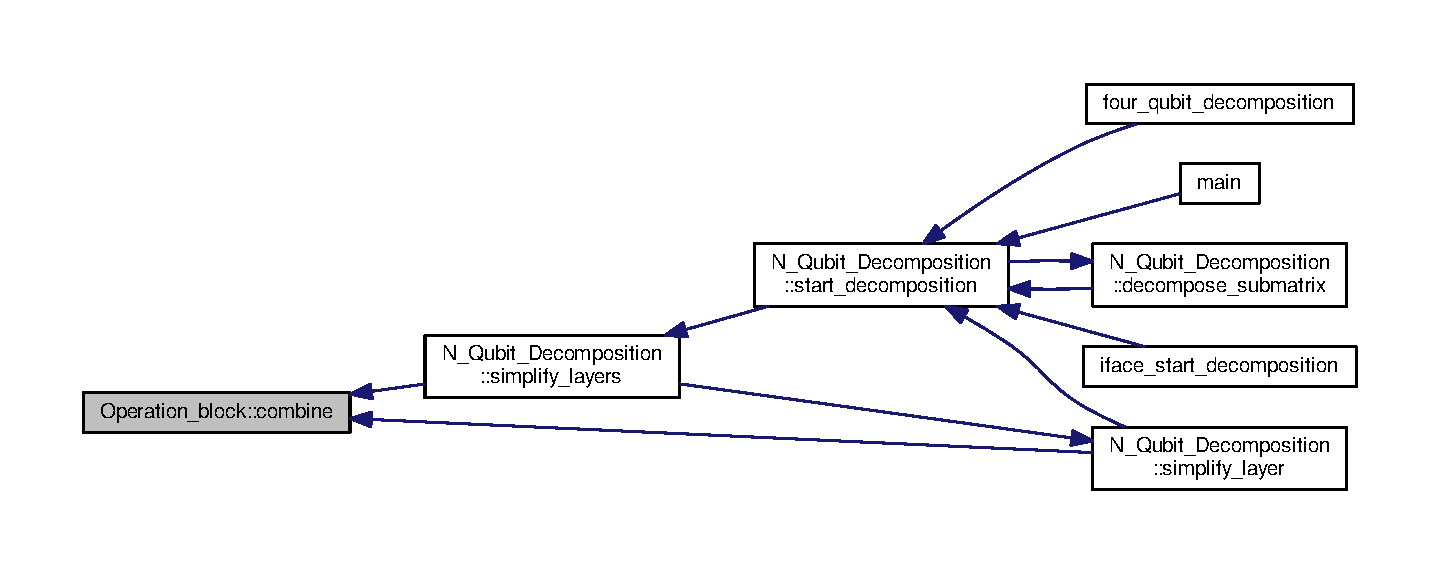
\includegraphics[width=350pt]{class_operation__block_a60062cf6f48ebfdcaae9db3367a66147_icgraph}
\end{center}
\end{figure}


\index{Decomposition\+\_\+\+Base@{Decomposition\+\_\+\+Base}!combine@{combine}}
\index{combine@{combine}!Decomposition\+\_\+\+Base@{Decomposition\+\_\+\+Base}}
\subsubsection[{\texorpdfstring{combine(\+Operation\+\_\+block $\ast$op\+\_\+block)}{combine(Operation_block *op_block)}}]{\setlength{\rightskip}{0pt plus 5cm}void Operation\+\_\+block\+::combine (
\begin{DoxyParamCaption}
\item[{{\bf Operation\+\_\+block} $\ast$}]{op\+\_\+block}
\end{DoxyParamCaption}
)\hspace{0.3cm}{\ttfamily [inherited]}}\hypertarget{class_operation__block_a60062cf6f48ebfdcaae9db3367a66147}{}\label{class_operation__block_a60062cf6f48ebfdcaae9db3367a66147}


Call to append the operations of an operation block to the current block. 


\begin{DoxyParams}{Parameters}
{\em op\+\_\+block} & A pointer to an instance of class \hyperlink{class_operation__block}{Operation\+\_\+block} \\
\hline
\end{DoxyParams}
\index{Decomposition\+\_\+\+Base@{Decomposition\+\_\+\+Base}!finalize\+\_\+decomposition@{finalize\+\_\+decomposition}}
\index{finalize\+\_\+decomposition@{finalize\+\_\+decomposition}!Decomposition\+\_\+\+Base@{Decomposition\+\_\+\+Base}}
\subsubsection[{\texorpdfstring{finalize\+\_\+decomposition()}{finalize_decomposition()}}]{\setlength{\rightskip}{0pt plus 5cm}void Decomposition\+\_\+\+Base\+::finalize\+\_\+decomposition (
\begin{DoxyParamCaption}
{}
\end{DoxyParamCaption}
)}\hypertarget{class_decomposition___base_a0cdd12741e72e2c074a188fe3867e6d5}{}\label{class_decomposition___base_a0cdd12741e72e2c074a188fe3867e6d5}


After the main optimalization problem is solved, the indepent qubits can be rotated into state $\vert$0$>$ by this def. 

The constructed operations are added to the array of operations needed to the decomposition of the input unitary. 

Definition at line 134 of file Decomposition\+\_\+\+Base.\+cpp.



Here is the call graph for this function\+:
\nopagebreak
\begin{figure}[H]
\begin{center}
\leavevmode
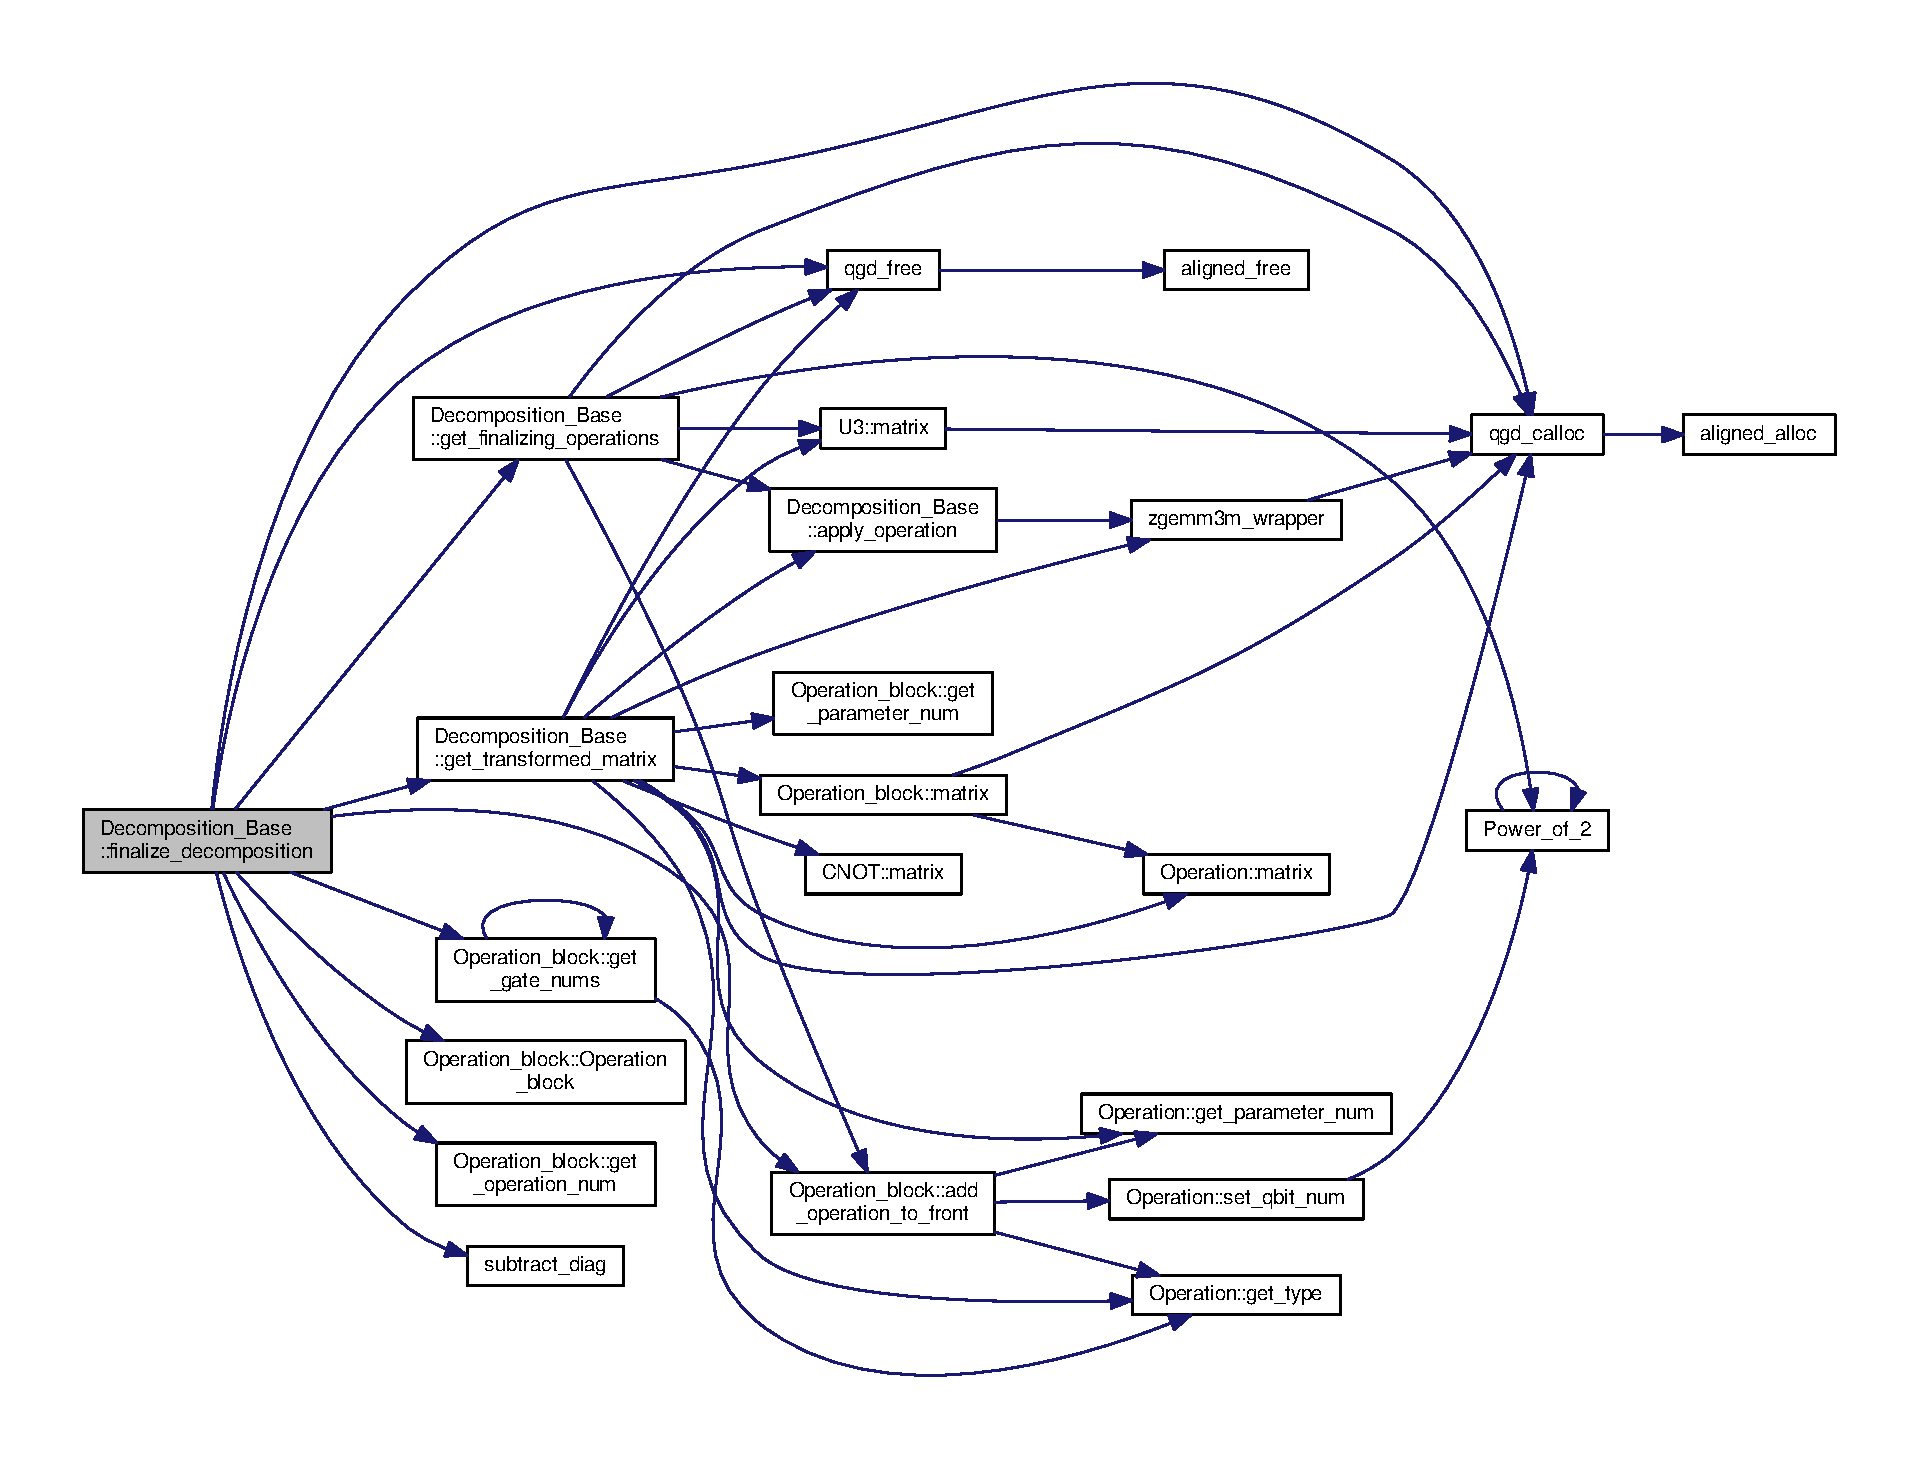
\includegraphics[width=350pt]{class_decomposition___base_a0cdd12741e72e2c074a188fe3867e6d5_cgraph}
\end{center}
\end{figure}




Here is the caller graph for this function\+:
\nopagebreak
\begin{figure}[H]
\begin{center}
\leavevmode
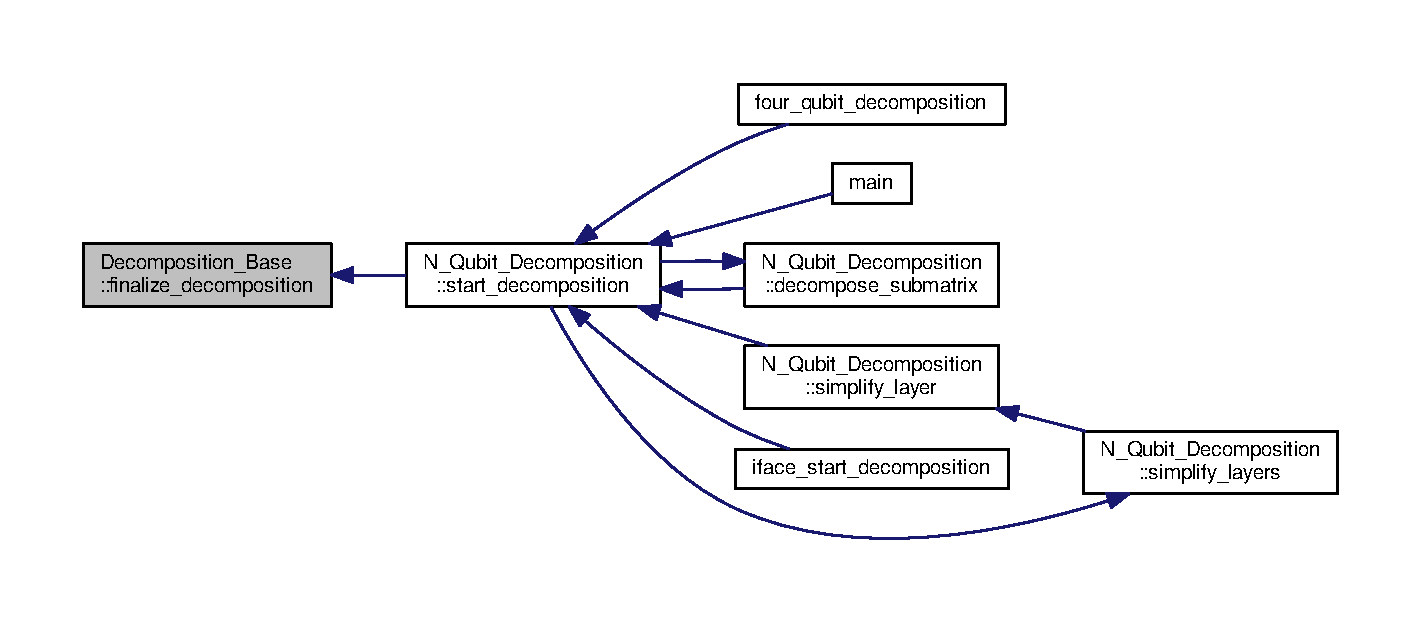
\includegraphics[width=350pt]{class_decomposition___base_a0cdd12741e72e2c074a188fe3867e6d5_icgraph}
\end{center}
\end{figure}


\index{Decomposition\+\_\+\+Base@{Decomposition\+\_\+\+Base}!finalize\+\_\+decomposition@{finalize\+\_\+decomposition}}
\index{finalize\+\_\+decomposition@{finalize\+\_\+decomposition}!Decomposition\+\_\+\+Base@{Decomposition\+\_\+\+Base}}
\subsubsection[{\texorpdfstring{finalize\+\_\+decomposition()}{finalize_decomposition()}}]{\setlength{\rightskip}{0pt plus 5cm}void Decomposition\+\_\+\+Base\+::finalize\+\_\+decomposition (
\begin{DoxyParamCaption}
{}
\end{DoxyParamCaption}
)}\hypertarget{class_decomposition___base_a0cdd12741e72e2c074a188fe3867e6d5}{}\label{class_decomposition___base_a0cdd12741e72e2c074a188fe3867e6d5}


After the main optimalization problem is solved, the indepent qubits can be rotated into state $\vert$0$>$ by this def. 

The constructed operations are added to the array of operations needed to the decomposition of the input unitary. \index{Decomposition\+\_\+\+Base@{Decomposition\+\_\+\+Base}!get\+\_\+control\+\_\+qbit@{get\+\_\+control\+\_\+qbit}}
\index{get\+\_\+control\+\_\+qbit@{get\+\_\+control\+\_\+qbit}!Decomposition\+\_\+\+Base@{Decomposition\+\_\+\+Base}}
\subsubsection[{\texorpdfstring{get\+\_\+control\+\_\+qbit()}{get_control_qbit()}}]{\setlength{\rightskip}{0pt plus 5cm}int Operation\+::get\+\_\+control\+\_\+qbit (
\begin{DoxyParamCaption}
{}
\end{DoxyParamCaption}
)\hspace{0.3cm}{\ttfamily [inherited]}}\hypertarget{class_operation_a2e9b60d334a0e0c99dede014ac989d0a}{}\label{class_operation_a2e9b60d334a0e0c99dede014ac989d0a}


Call to get the index of the control qubit. 

\begin{DoxyReturn}{Returns}
Return with the index of the control qubit (return with -\/1 if control qubit was not set) 
\end{DoxyReturn}


Definition at line 178 of file Operation.\+cpp.



Here is the caller graph for this function\+:
\nopagebreak
\begin{figure}[H]
\begin{center}
\leavevmode
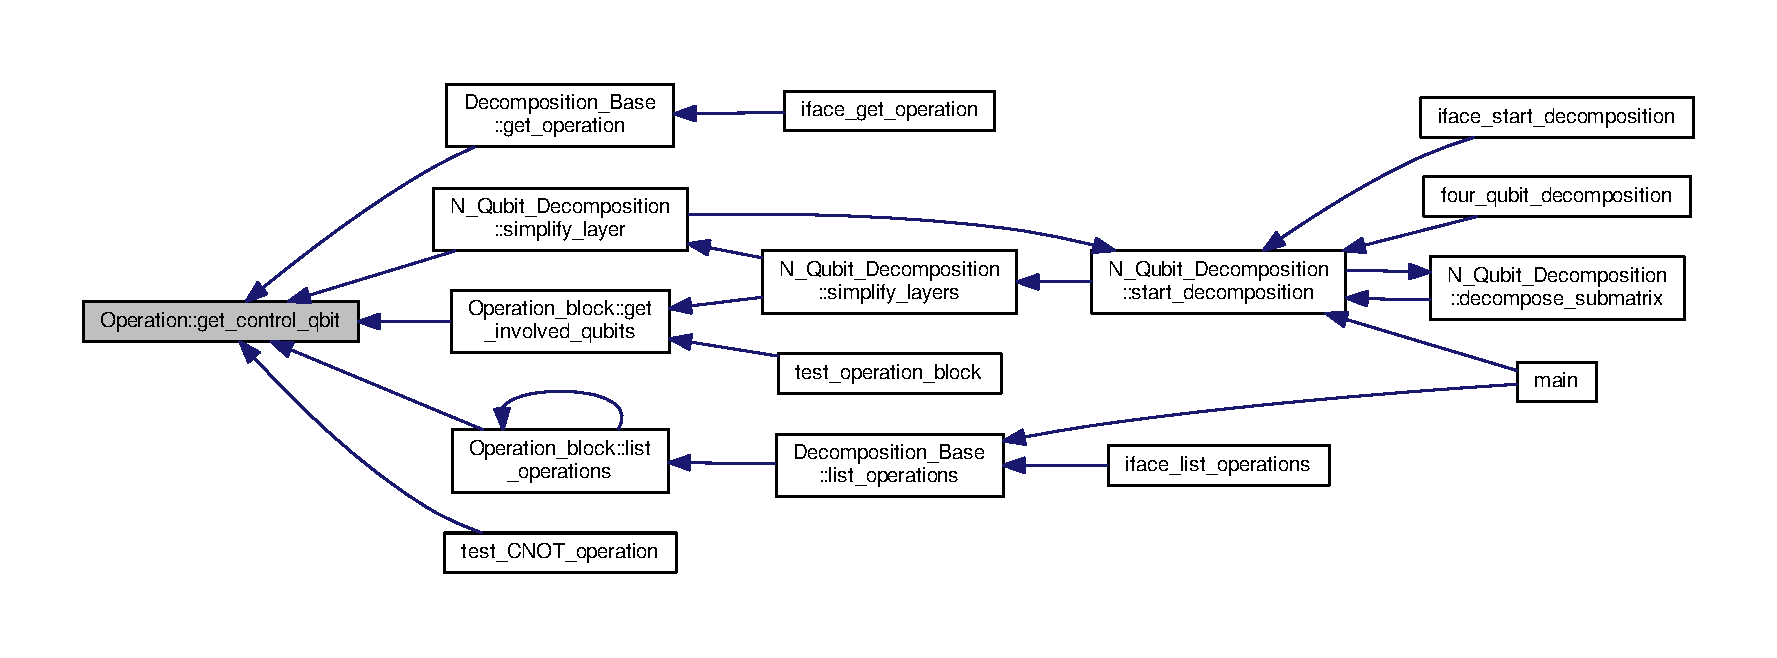
\includegraphics[width=350pt]{class_operation_a2e9b60d334a0e0c99dede014ac989d0a_icgraph}
\end{center}
\end{figure}


\index{Decomposition\+\_\+\+Base@{Decomposition\+\_\+\+Base}!get\+\_\+control\+\_\+qbit@{get\+\_\+control\+\_\+qbit}}
\index{get\+\_\+control\+\_\+qbit@{get\+\_\+control\+\_\+qbit}!Decomposition\+\_\+\+Base@{Decomposition\+\_\+\+Base}}
\subsubsection[{\texorpdfstring{get\+\_\+control\+\_\+qbit()}{get_control_qbit()}}]{\setlength{\rightskip}{0pt plus 5cm}int Operation\+::get\+\_\+control\+\_\+qbit (
\begin{DoxyParamCaption}
{}
\end{DoxyParamCaption}
)\hspace{0.3cm}{\ttfamily [inherited]}}\hypertarget{class_operation_a2e9b60d334a0e0c99dede014ac989d0a}{}\label{class_operation_a2e9b60d334a0e0c99dede014ac989d0a}


Call to get the index of the control qubit. 

\begin{DoxyReturn}{Returns}
Return with the index of the control qubit (return with -\/1 if control qubit was not set) 
\end{DoxyReturn}
\index{Decomposition\+\_\+\+Base@{Decomposition\+\_\+\+Base}!get\+\_\+decomposed\+\_\+matrix@{get\+\_\+decomposed\+\_\+matrix}}
\index{get\+\_\+decomposed\+\_\+matrix@{get\+\_\+decomposed\+\_\+matrix}!Decomposition\+\_\+\+Base@{Decomposition\+\_\+\+Base}}
\subsubsection[{\texorpdfstring{get\+\_\+decomposed\+\_\+matrix()}{get_decomposed_matrix()}}]{\setlength{\rightskip}{0pt plus 5cm}{\bf Q\+G\+D\+\_\+\+Complex16} $\ast$ Decomposition\+\_\+\+Base\+::get\+\_\+decomposed\+\_\+matrix (
\begin{DoxyParamCaption}
{}
\end{DoxyParamCaption}
)}\hypertarget{class_decomposition___base_a40154345dce69fd5a9cb28c0b677746b}{}\label{class_decomposition___base_a40154345dce69fd5a9cb28c0b677746b}


Calculate the decomposed matrix resulted by the effect of the optimized operations on the unitary . 

\begin{DoxyReturn}{Returns}
Returns with the decomposed matrix. 
\end{DoxyReturn}


Definition at line 828 of file Decomposition\+\_\+\+Base.\+cpp.



Here is the call graph for this function\+:
\nopagebreak
\begin{figure}[H]
\begin{center}
\leavevmode
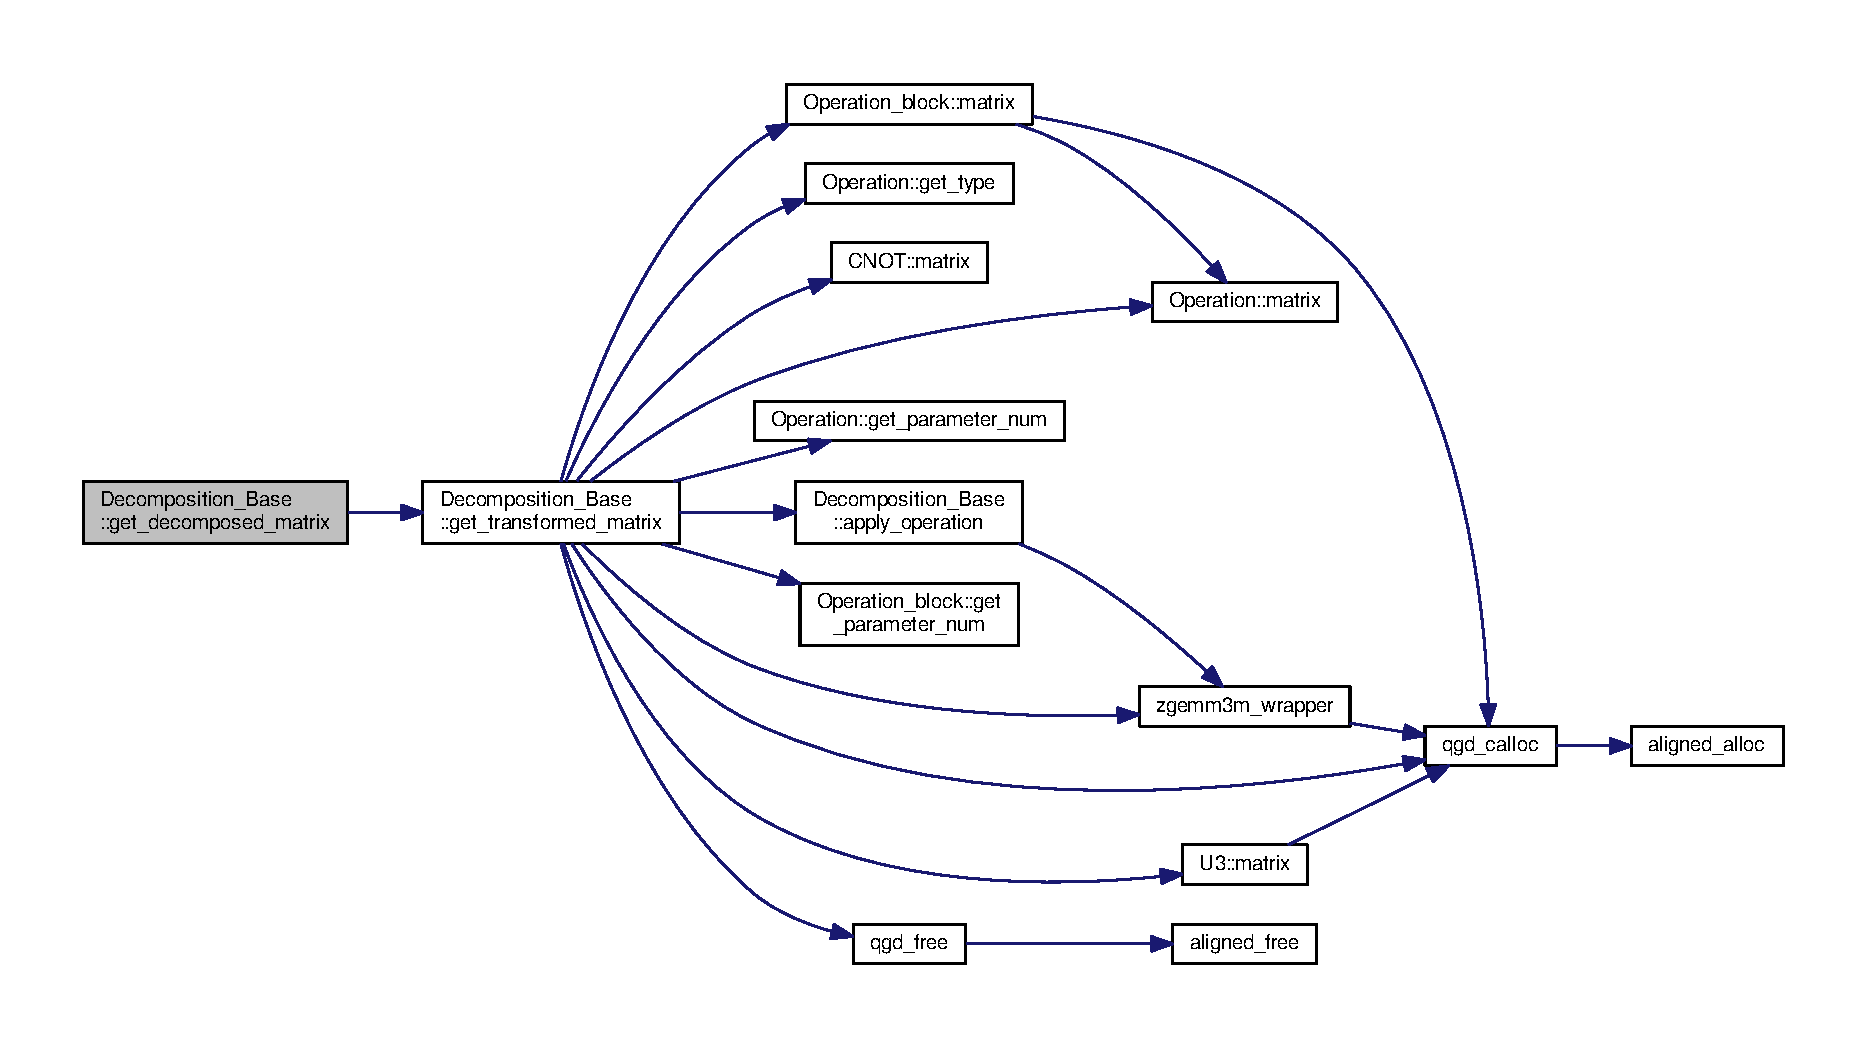
\includegraphics[width=350pt]{class_decomposition___base_a40154345dce69fd5a9cb28c0b677746b_cgraph}
\end{center}
\end{figure}


\index{Decomposition\+\_\+\+Base@{Decomposition\+\_\+\+Base}!get\+\_\+decomposed\+\_\+matrix@{get\+\_\+decomposed\+\_\+matrix}}
\index{get\+\_\+decomposed\+\_\+matrix@{get\+\_\+decomposed\+\_\+matrix}!Decomposition\+\_\+\+Base@{Decomposition\+\_\+\+Base}}
\subsubsection[{\texorpdfstring{get\+\_\+decomposed\+\_\+matrix()}{get_decomposed_matrix()}}]{\setlength{\rightskip}{0pt plus 5cm}{\bf Q\+G\+D\+\_\+\+Complex16}$\ast$ Decomposition\+\_\+\+Base\+::get\+\_\+decomposed\+\_\+matrix (
\begin{DoxyParamCaption}
{}
\end{DoxyParamCaption}
)}\hypertarget{class_decomposition___base_ae71eaec68c77e79716cae632f97d42eb}{}\label{class_decomposition___base_ae71eaec68c77e79716cae632f97d42eb}


Calculate the decomposed matrix resulted by the effect of the optimized operations on the unitary . 

\begin{DoxyReturn}{Returns}
Returns with the decomposed matrix. 
\end{DoxyReturn}
\index{Decomposition\+\_\+\+Base@{Decomposition\+\_\+\+Base}!get\+\_\+finalizing\+\_\+operations@{get\+\_\+finalizing\+\_\+operations}}
\index{get\+\_\+finalizing\+\_\+operations@{get\+\_\+finalizing\+\_\+operations}!Decomposition\+\_\+\+Base@{Decomposition\+\_\+\+Base}}
\subsubsection[{\texorpdfstring{get\+\_\+finalizing\+\_\+operations(\+Q\+G\+D\+\_\+\+Complex16 $\ast$mtx, Operation\+\_\+block $\ast$finalizing\+\_\+operations, double $\ast$finalizing\+\_\+parameters)}{get_finalizing_operations(QGD_Complex16 *mtx, Operation_block *finalizing_operations, double *finalizing_parameters)}}]{\setlength{\rightskip}{0pt plus 5cm}void Decomposition\+\_\+\+Base\+::get\+\_\+finalizing\+\_\+operations (
\begin{DoxyParamCaption}
\item[{{\bf Q\+G\+D\+\_\+\+Complex16} $\ast$}]{mtx, }
\item[{{\bf Operation\+\_\+block} $\ast$}]{finalizing\+\_\+operations, }
\item[{double $\ast$}]{finalizing\+\_\+parameters}
\end{DoxyParamCaption}
)}\hypertarget{class_decomposition___base_a9832cc5308c00b73d3e6bc331a77c7f7}{}\label{class_decomposition___base_a9832cc5308c00b73d3e6bc331a77c7f7}


This method determine the operations needed to rotate the indepent qubits into the state $\vert$0$>$ 


\begin{DoxyParams}{Parameters}
{\em mtx} & The unitary describing indepent qubits. The resulting matrix is returned by this pointer \\
\hline
{\em finalizing\+\_\+operations} & Pointer pointig to a block of operations containing the final operations. \\
\hline
{\em finalizing\+\_\+parameters} & Parameters corresponding to the finalizing operations. \\
\hline
\end{DoxyParams}


Definition at line 202 of file Decomposition\+\_\+\+Base.\+cpp.



Here is the call graph for this function\+:
\nopagebreak
\begin{figure}[H]
\begin{center}
\leavevmode
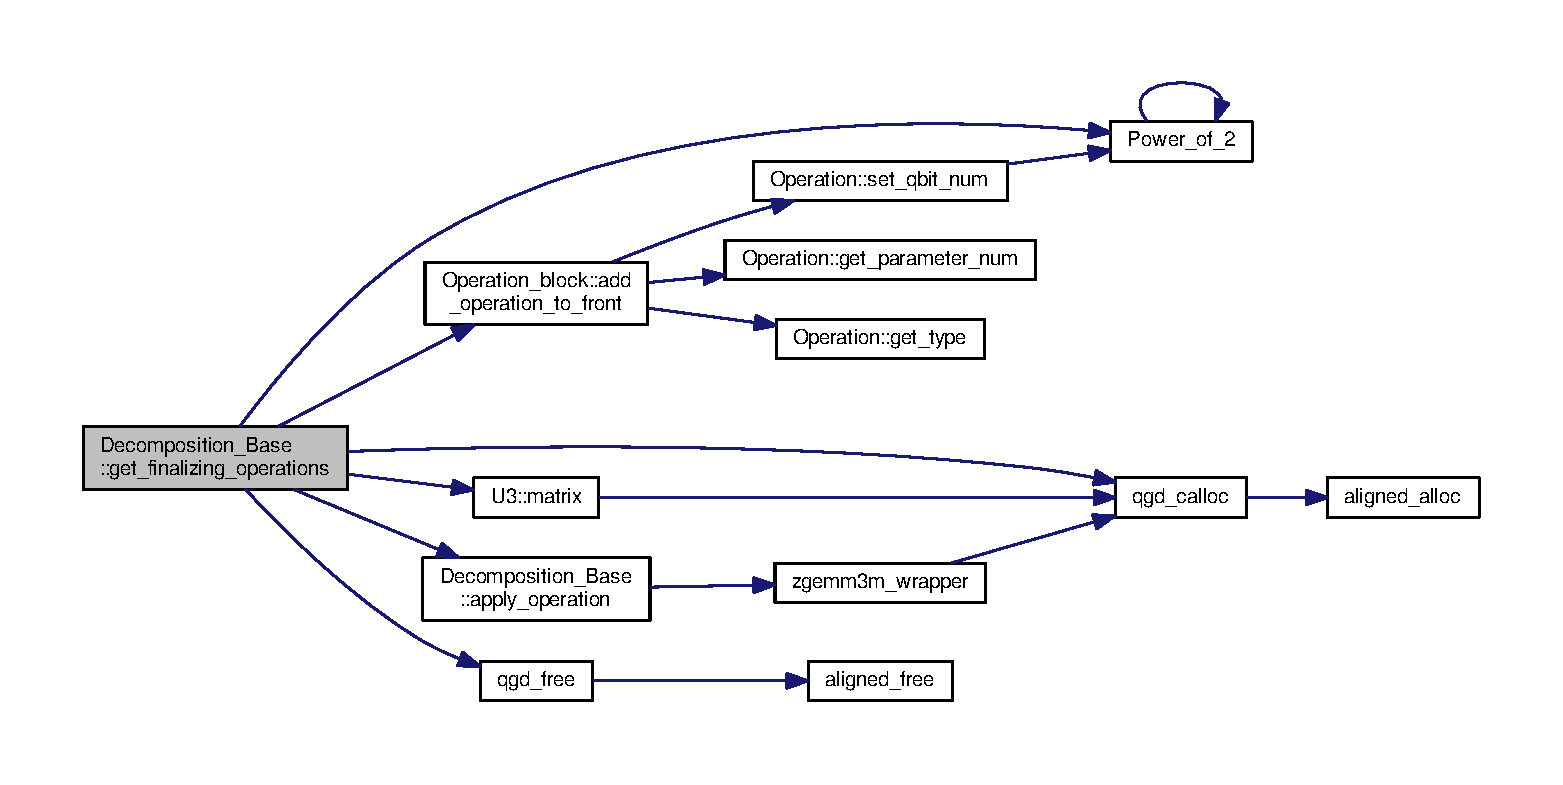
\includegraphics[width=350pt]{class_decomposition___base_a9832cc5308c00b73d3e6bc331a77c7f7_cgraph}
\end{center}
\end{figure}




Here is the caller graph for this function\+:
\nopagebreak
\begin{figure}[H]
\begin{center}
\leavevmode
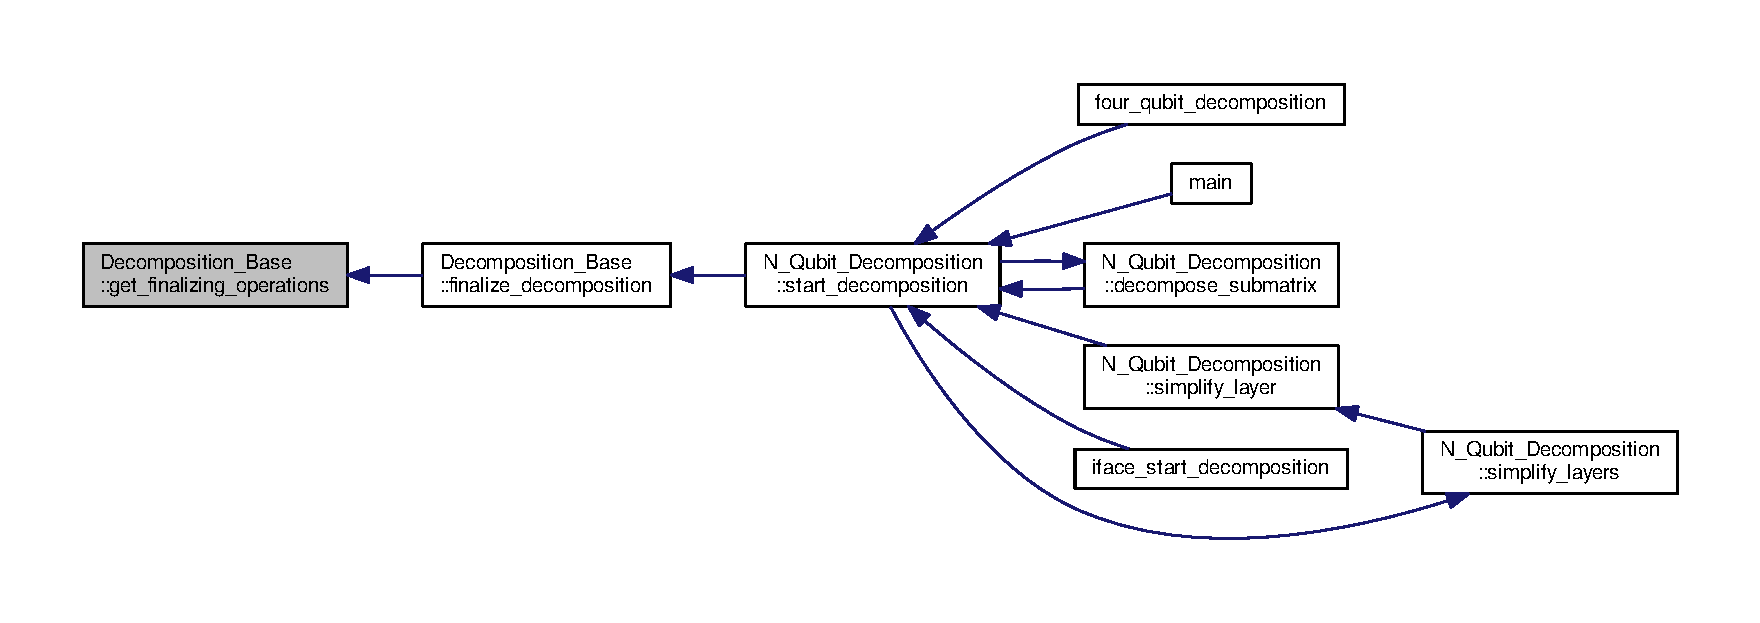
\includegraphics[width=350pt]{class_decomposition___base_a9832cc5308c00b73d3e6bc331a77c7f7_icgraph}
\end{center}
\end{figure}


\index{Decomposition\+\_\+\+Base@{Decomposition\+\_\+\+Base}!get\+\_\+finalizing\+\_\+operations@{get\+\_\+finalizing\+\_\+operations}}
\index{get\+\_\+finalizing\+\_\+operations@{get\+\_\+finalizing\+\_\+operations}!Decomposition\+\_\+\+Base@{Decomposition\+\_\+\+Base}}
\subsubsection[{\texorpdfstring{get\+\_\+finalizing\+\_\+operations(\+Q\+G\+D\+\_\+\+Complex16 $\ast$mtx, Operation\+\_\+block $\ast$finalizing\+\_\+operations, double $\ast$finalizing\+\_\+parameters)}{get_finalizing_operations(QGD_Complex16 *mtx, Operation_block *finalizing_operations, double *finalizing_parameters)}}]{\setlength{\rightskip}{0pt plus 5cm}void Decomposition\+\_\+\+Base\+::get\+\_\+finalizing\+\_\+operations (
\begin{DoxyParamCaption}
\item[{{\bf Q\+G\+D\+\_\+\+Complex16} $\ast$}]{mtx, }
\item[{{\bf Operation\+\_\+block} $\ast$}]{finalizing\+\_\+operations, }
\item[{double $\ast$}]{finalizing\+\_\+parameters}
\end{DoxyParamCaption}
)}\hypertarget{class_decomposition___base_a9832cc5308c00b73d3e6bc331a77c7f7}{}\label{class_decomposition___base_a9832cc5308c00b73d3e6bc331a77c7f7}


This method determine the operations needed to rotate the indepent qubits into the state $\vert$0$>$ 


\begin{DoxyParams}{Parameters}
{\em mtx} & The unitary describing indepent qubits. The resulting matrix is returned by this pointer \\
\hline
{\em finalizing\+\_\+operations} & Pointer pointig to a block of operations containing the final operations. \\
\hline
{\em finalizing\+\_\+parameters} & Parameters corresponding to the finalizing operations. \\
\hline
\end{DoxyParams}
\index{Decomposition\+\_\+\+Base@{Decomposition\+\_\+\+Base}!get\+\_\+gate\+\_\+nums@{get\+\_\+gate\+\_\+nums}}
\index{get\+\_\+gate\+\_\+nums@{get\+\_\+gate\+\_\+nums}!Decomposition\+\_\+\+Base@{Decomposition\+\_\+\+Base}}
\subsubsection[{\texorpdfstring{get\+\_\+gate\+\_\+nums()}{get_gate_nums()}}]{\setlength{\rightskip}{0pt plus 5cm}{\bf gates\+\_\+num} Operation\+\_\+block\+::get\+\_\+gate\+\_\+nums (
\begin{DoxyParamCaption}
{}
\end{DoxyParamCaption}
)\hspace{0.3cm}{\ttfamily [inherited]}}\hypertarget{class_operation__block_ac39ab782da3e34c8ec4acf6181fbc5f7}{}\label{class_operation__block_ac39ab782da3e34c8ec4acf6181fbc5f7}


Call to get the number of the individual gate types in the list of operations. 

\begin{DoxyReturn}{Returns}
Returns with an instance  describing the number of the individual gate types 
\end{DoxyReturn}


Definition at line 409 of file Operation\+\_\+block.\+cpp.



Here is the call graph for this function\+:
\nopagebreak
\begin{figure}[H]
\begin{center}
\leavevmode
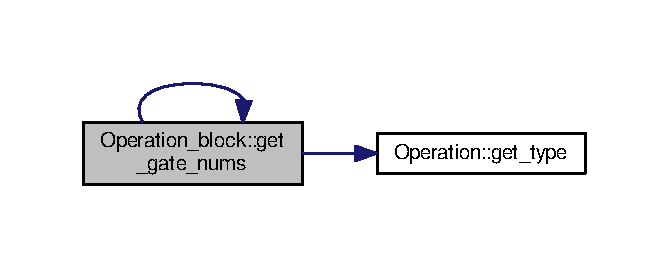
\includegraphics[width=321pt]{class_operation__block_ac39ab782da3e34c8ec4acf6181fbc5f7_cgraph}
\end{center}
\end{figure}




Here is the caller graph for this function\+:
\nopagebreak
\begin{figure}[H]
\begin{center}
\leavevmode
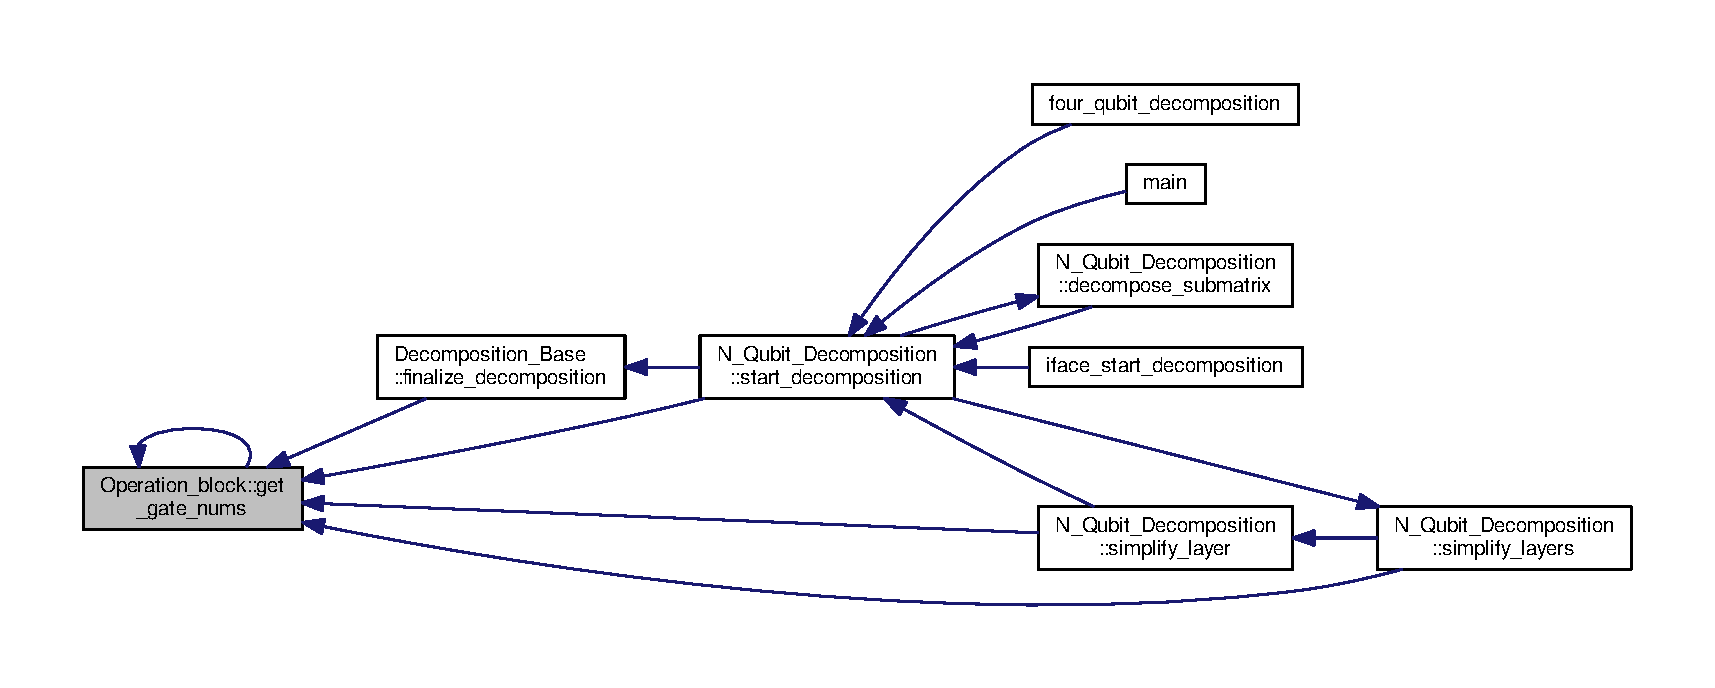
\includegraphics[width=350pt]{class_operation__block_ac39ab782da3e34c8ec4acf6181fbc5f7_icgraph}
\end{center}
\end{figure}


\index{Decomposition\+\_\+\+Base@{Decomposition\+\_\+\+Base}!get\+\_\+gate\+\_\+nums@{get\+\_\+gate\+\_\+nums}}
\index{get\+\_\+gate\+\_\+nums@{get\+\_\+gate\+\_\+nums}!Decomposition\+\_\+\+Base@{Decomposition\+\_\+\+Base}}
\subsubsection[{\texorpdfstring{get\+\_\+gate\+\_\+nums()}{get_gate_nums()}}]{\setlength{\rightskip}{0pt plus 5cm}{\bf gates\+\_\+num} Operation\+\_\+block\+::get\+\_\+gate\+\_\+nums (
\begin{DoxyParamCaption}
{}
\end{DoxyParamCaption}
)\hspace{0.3cm}{\ttfamily [inherited]}}\hypertarget{class_operation__block_ac39ab782da3e34c8ec4acf6181fbc5f7}{}\label{class_operation__block_ac39ab782da3e34c8ec4acf6181fbc5f7}


Call to get the number of the individual gate types in the list of operations. 

\begin{DoxyReturn}{Returns}
Returns with an instance  describing the number of the individual gate types 
\end{DoxyReturn}
\index{Decomposition\+\_\+\+Base@{Decomposition\+\_\+\+Base}!get\+\_\+involved\+\_\+qubits@{get\+\_\+involved\+\_\+qubits}}
\index{get\+\_\+involved\+\_\+qubits@{get\+\_\+involved\+\_\+qubits}!Decomposition\+\_\+\+Base@{Decomposition\+\_\+\+Base}}
\subsubsection[{\texorpdfstring{get\+\_\+involved\+\_\+qubits()}{get_involved_qubits()}}]{\setlength{\rightskip}{0pt plus 5cm}std\+::vector$<$ int $>$ Operation\+\_\+block\+::get\+\_\+involved\+\_\+qubits (
\begin{DoxyParamCaption}
{}
\end{DoxyParamCaption}
)\hspace{0.3cm}{\ttfamily [inherited]}}\hypertarget{class_operation__block_a92e4f0566e4b36830652729377a8e936}{}\label{class_operation__block_a92e4f0566e4b36830652729377a8e936}


Call to get the qubits involved in the operations stored in the block of operations. 

\begin{DoxyReturn}{Returns}
Return with a list of the invovled qubits 
\end{DoxyReturn}


Definition at line 592 of file Operation\+\_\+block.\+cpp.



Here is the call graph for this function\+:
\nopagebreak
\begin{figure}[H]
\begin{center}
\leavevmode
\includegraphics[width=350pt]{class_operation__block_a92e4f0566e4b36830652729377a8e936_cgraph}
\end{center}
\end{figure}




Here is the caller graph for this function\+:
\nopagebreak
\begin{figure}[H]
\begin{center}
\leavevmode
\includegraphics[width=350pt]{class_operation__block_a92e4f0566e4b36830652729377a8e936_icgraph}
\end{center}
\end{figure}


\index{Decomposition\+\_\+\+Base@{Decomposition\+\_\+\+Base}!get\+\_\+involved\+\_\+qubits@{get\+\_\+involved\+\_\+qubits}}
\index{get\+\_\+involved\+\_\+qubits@{get\+\_\+involved\+\_\+qubits}!Decomposition\+\_\+\+Base@{Decomposition\+\_\+\+Base}}
\subsubsection[{\texorpdfstring{get\+\_\+involved\+\_\+qubits()}{get_involved_qubits()}}]{\setlength{\rightskip}{0pt plus 5cm}std\+::vector$<$int$>$ Operation\+\_\+block\+::get\+\_\+involved\+\_\+qubits (
\begin{DoxyParamCaption}
{}
\end{DoxyParamCaption}
)\hspace{0.3cm}{\ttfamily [inherited]}}\hypertarget{class_operation__block_aebdbb71e02ff6826d967d55f4cd4db28}{}\label{class_operation__block_aebdbb71e02ff6826d967d55f4cd4db28}


Call to get the qubits involved in the operations stored in the block of operations. 

\begin{DoxyReturn}{Returns}
Return with a list of the invovled qubits 
\end{DoxyReturn}
\index{Decomposition\+\_\+\+Base@{Decomposition\+\_\+\+Base}!get\+\_\+matrices@{get\+\_\+matrices}}
\index{get\+\_\+matrices@{get\+\_\+matrices}!Decomposition\+\_\+\+Base@{Decomposition\+\_\+\+Base}}
\subsubsection[{\texorpdfstring{get\+\_\+matrices(const double $\ast$parameters)}{get_matrices(const double *parameters)}}]{\setlength{\rightskip}{0pt plus 5cm}std\+::vector$<$ {\bf Q\+G\+D\+\_\+\+Complex16} $\ast$ $>$ Operation\+\_\+block\+::get\+\_\+matrices (
\begin{DoxyParamCaption}
\item[{const double $\ast$}]{parameters}
\end{DoxyParamCaption}
)\hspace{0.3cm}{\ttfamily [inherited]}}\hypertarget{class_operation__block_aedddbc5242eab7c00125359a835ac53d}{}\label{class_operation__block_aedddbc5242eab7c00125359a835ac53d}


Call to get the list of matrix representation of the operations grouped in the block. 


\begin{DoxyParams}{Parameters}
{\em parameters} & Array of parameters to calculate the matrix of the operation block \\
\hline
\end{DoxyParams}
\begin{DoxyReturn}{Returns}
Returns with the list of the operations 
\end{DoxyReturn}


Definition at line 214 of file Operation\+\_\+block.\+cpp.



Here is the call graph for this function\+:
\nopagebreak
\begin{figure}[H]
\begin{center}
\leavevmode
\includegraphics[width=350pt]{class_operation__block_aedddbc5242eab7c00125359a835ac53d_cgraph}
\end{center}
\end{figure}




Here is the caller graph for this function\+:
\nopagebreak
\begin{figure}[H]
\begin{center}
\leavevmode
\includegraphics[width=339pt]{class_operation__block_aedddbc5242eab7c00125359a835ac53d_icgraph}
\end{center}
\end{figure}


\index{Decomposition\+\_\+\+Base@{Decomposition\+\_\+\+Base}!get\+\_\+matrices@{get\+\_\+matrices}}
\index{get\+\_\+matrices@{get\+\_\+matrices}!Decomposition\+\_\+\+Base@{Decomposition\+\_\+\+Base}}
\subsubsection[{\texorpdfstring{get\+\_\+matrices(const double $\ast$parameters)}{get_matrices(const double *parameters)}}]{\setlength{\rightskip}{0pt plus 5cm}std\+::vector$<${\bf Q\+G\+D\+\_\+\+Complex16}$\ast$$>$ Operation\+\_\+block\+::get\+\_\+matrices (
\begin{DoxyParamCaption}
\item[{const double $\ast$}]{parameters}
\end{DoxyParamCaption}
)\hspace{0.3cm}{\ttfamily [inherited]}}\hypertarget{class_operation__block_af3e794fd9a409978a414af539ad23320}{}\label{class_operation__block_af3e794fd9a409978a414af539ad23320}


Call to get the list of matrix representation of the operations grouped in the block. 


\begin{DoxyParams}{Parameters}
{\em parameters} & Array of parameters to calculate the matrix of the operation block \\
\hline
\end{DoxyParams}
\begin{DoxyReturn}{Returns}
Returns with the list of the operations 
\end{DoxyReturn}
\index{Decomposition\+\_\+\+Base@{Decomposition\+\_\+\+Base}!get\+\_\+operation@{get\+\_\+operation}}
\index{get\+\_\+operation@{get\+\_\+operation}!Decomposition\+\_\+\+Base@{Decomposition\+\_\+\+Base}}
\subsubsection[{\texorpdfstring{get\+\_\+operation(int n, operation\+\_\+type \&type, int \&target\+\_\+qbit, int \&control\+\_\+qbit, double $\ast$parameters)}{get_operation(int n, operation_type &type, int &target_qbit, int &control_qbit, double *parameters)}}]{\setlength{\rightskip}{0pt plus 5cm}int Decomposition\+\_\+\+Base\+::get\+\_\+operation (
\begin{DoxyParamCaption}
\item[{int}]{n, }
\item[{{\bf operation\+\_\+type} \&}]{type, }
\item[{int \&}]{target\+\_\+qbit, }
\item[{int \&}]{control\+\_\+qbit, }
\item[{double $\ast$}]{parameters}
\end{DoxyParamCaption}
)}\hypertarget{class_decomposition___base_a64e2b692d38fe3ccbd49708d8fa24493}{}\label{class_decomposition___base_a64e2b692d38fe3ccbd49708d8fa24493}


Call to prepare the optimized operations to export. 


\begin{DoxyParams}{Parameters}
{\em n} & Integer labeling the n-\/th oepration (n$>$=0). \\
\hline
{\em block\+\_\+op} & A pointer to a block of operations \\
\hline
{\em parameters} & The parameters of the operations \\
\hline
\end{DoxyParams}
\begin{DoxyReturn}{Returns}
Returns with 0 if the export of the n-\/th operation was successful. If the n-\/th operation does not exists, -\/1 is returned. If the operation is not allowed to be exported, i.\+e. it is not a \hyperlink{class_c_n_o_t}{C\+N\+OT} or \hyperlink{class_u3}{U3} operation, then -\/2 is returned. 
\end{DoxyReturn}
\index{Decomposition\+\_\+\+Base@{Decomposition\+\_\+\+Base}!get\+\_\+operation@{get\+\_\+operation}}
\index{get\+\_\+operation@{get\+\_\+operation}!Decomposition\+\_\+\+Base@{Decomposition\+\_\+\+Base}}
\subsubsection[{\texorpdfstring{get\+\_\+operation(int n, operation\+\_\+type \&type, int \&target\+\_\+qbit, int \&control\+\_\+qbit, double $\ast$parameters)}{get_operation(int n, operation_type &type, int &target_qbit, int &control_qbit, double *parameters)}}]{\setlength{\rightskip}{0pt plus 5cm}int Decomposition\+\_\+\+Base\+::get\+\_\+operation (
\begin{DoxyParamCaption}
\item[{int}]{n, }
\item[{{\bf operation\+\_\+type} \&}]{type, }
\item[{int \&}]{target\+\_\+qbit, }
\item[{int \&}]{control\+\_\+qbit, }
\item[{double $\ast$}]{parameters}
\end{DoxyParamCaption}
)}\hypertarget{class_decomposition___base_a64e2b692d38fe3ccbd49708d8fa24493}{}\label{class_decomposition___base_a64e2b692d38fe3ccbd49708d8fa24493}


Call to prepare the optimized operations to export. 


\begin{DoxyParams}{Parameters}
{\em n} & Integer labeling the n-\/th oepration (n$>$=0). \\
\hline
{\em block\+\_\+op} & A pointer to a block of operations \\
\hline
{\em parameters} & The parameters of the operations \\
\hline
\end{DoxyParams}
\begin{DoxyReturn}{Returns}
Returns with 0 if the export of the n-\/th operation was successful. If the n-\/th operation does not exists, -\/1 is returned. If the operation is not allowed to be exported, i.\+e. it is not a \hyperlink{class_c_n_o_t}{C\+N\+OT} or \hyperlink{class_u3}{U3} operation, then -\/2 is returned. 
\end{DoxyReturn}


Definition at line 1065 of file Decomposition\+\_\+\+Base.\+cpp.



Here is the call graph for this function\+:
\nopagebreak
\begin{figure}[H]
\begin{center}
\leavevmode
\includegraphics[width=350pt]{class_decomposition___base_a64e2b692d38fe3ccbd49708d8fa24493_cgraph}
\end{center}
\end{figure}




Here is the caller graph for this function\+:
\nopagebreak
\begin{figure}[H]
\begin{center}
\leavevmode
\includegraphics[width=326pt]{class_decomposition___base_a64e2b692d38fe3ccbd49708d8fa24493_icgraph}
\end{center}
\end{figure}


\index{Decomposition\+\_\+\+Base@{Decomposition\+\_\+\+Base}!get\+\_\+operation\+\_\+num@{get\+\_\+operation\+\_\+num}}
\index{get\+\_\+operation\+\_\+num@{get\+\_\+operation\+\_\+num}!Decomposition\+\_\+\+Base@{Decomposition\+\_\+\+Base}}
\subsubsection[{\texorpdfstring{get\+\_\+operation\+\_\+num()}{get_operation_num()}}]{\setlength{\rightskip}{0pt plus 5cm}int Operation\+\_\+block\+::get\+\_\+operation\+\_\+num (
\begin{DoxyParamCaption}
{}
\end{DoxyParamCaption}
)\hspace{0.3cm}{\ttfamily [inherited]}}\hypertarget{class_operation__block_a27592a2d25c7e74416de2b9d7997efca}{}\label{class_operation__block_a27592a2d25c7e74416de2b9d7997efca}


Call to get the number of operations grouped in the block. 

\begin{DoxyReturn}{Returns}
Return with the number of the operations grouped in the operation block. 
\end{DoxyReturn}


Definition at line 458 of file Operation\+\_\+block.\+cpp.



Here is the caller graph for this function\+:
\nopagebreak
\begin{figure}[H]
\begin{center}
\leavevmode
\includegraphics[width=350pt]{class_operation__block_a27592a2d25c7e74416de2b9d7997efca_icgraph}
\end{center}
\end{figure}


\index{Decomposition\+\_\+\+Base@{Decomposition\+\_\+\+Base}!get\+\_\+operation\+\_\+num@{get\+\_\+operation\+\_\+num}}
\index{get\+\_\+operation\+\_\+num@{get\+\_\+operation\+\_\+num}!Decomposition\+\_\+\+Base@{Decomposition\+\_\+\+Base}}
\subsubsection[{\texorpdfstring{get\+\_\+operation\+\_\+num()}{get_operation_num()}}]{\setlength{\rightskip}{0pt plus 5cm}int Operation\+\_\+block\+::get\+\_\+operation\+\_\+num (
\begin{DoxyParamCaption}
{}
\end{DoxyParamCaption}
)\hspace{0.3cm}{\ttfamily [inherited]}}\hypertarget{class_operation__block_a27592a2d25c7e74416de2b9d7997efca}{}\label{class_operation__block_a27592a2d25c7e74416de2b9d7997efca}


Call to get the number of operations grouped in the block. 

\begin{DoxyReturn}{Returns}
Return with the number of the operations grouped in the operation block. 
\end{DoxyReturn}
\index{Decomposition\+\_\+\+Base@{Decomposition\+\_\+\+Base}!get\+\_\+operation\+\_\+products@{get\+\_\+operation\+\_\+products}}
\index{get\+\_\+operation\+\_\+products@{get\+\_\+operation\+\_\+products}!Decomposition\+\_\+\+Base@{Decomposition\+\_\+\+Base}}
\subsubsection[{\texorpdfstring{get\+\_\+operation\+\_\+products(double $\ast$parameters, std\+::vector$<$ Operation $\ast$ $>$\+::iterator operations\+\_\+it, int num\+\_\+of\+\_\+operations)}{get_operation_products(double *parameters, std::vector< Operation * >::iterator operations_it, int num_of_operations)}}]{\setlength{\rightskip}{0pt plus 5cm}std\+::vector$<${\bf Q\+G\+D\+\_\+\+Complex16}$\ast$$>$ Decomposition\+\_\+\+Base\+::get\+\_\+operation\+\_\+products (
\begin{DoxyParamCaption}
\item[{double $\ast$}]{parameters, }
\item[{std\+::vector$<$ {\bf Operation} $\ast$ $>$\+::iterator}]{operations\+\_\+it, }
\item[{int}]{num\+\_\+of\+\_\+operations}
\end{DoxyParamCaption}
)}\hypertarget{class_decomposition___base_a7e6efc3b157653de20275e234d4df3d9}{}\label{class_decomposition___base_a7e6efc3b157653de20275e234d4df3d9}


Calculate the list of gate operation matrices such that the i$>$0-\/th element in the result list is the product of the operations of all 0$<$=n$<$i operations from the input list and the 0th element in the result list is the identity. 


\begin{DoxyParams}{Parameters}
{\em parameters} & An array containing the parameters of the \hyperlink{class_u3}{U3} operations. \\
\hline
{\em operations\+\_\+it} & An iterator pointing to the forst operation. \\
\hline
{\em num\+\_\+of\+\_\+operations} & The number of operations involved in the calculations \\
\hline
\end{DoxyParams}
\begin{DoxyReturn}{Returns}
Returns with a vector of the product matrices. 
\end{DoxyReturn}
\index{Decomposition\+\_\+\+Base@{Decomposition\+\_\+\+Base}!get\+\_\+operation\+\_\+products@{get\+\_\+operation\+\_\+products}}
\index{get\+\_\+operation\+\_\+products@{get\+\_\+operation\+\_\+products}!Decomposition\+\_\+\+Base@{Decomposition\+\_\+\+Base}}
\subsubsection[{\texorpdfstring{get\+\_\+operation\+\_\+products(double $\ast$parameters, std\+::vector$<$ Operation $\ast$ $>$\+::iterator operations\+\_\+it, int num\+\_\+of\+\_\+operations)}{get_operation_products(double *parameters, std::vector< Operation * >::iterator operations_it, int num_of_operations)}}]{\setlength{\rightskip}{0pt plus 5cm}std\+::vector$<$ {\bf Q\+G\+D\+\_\+\+Complex16} $\ast$ $>$ Decomposition\+\_\+\+Base\+::get\+\_\+operation\+\_\+products (
\begin{DoxyParamCaption}
\item[{double $\ast$}]{parameters, }
\item[{std\+::vector$<$ {\bf Operation} $\ast$ $>$\+::iterator}]{operations\+\_\+it, }
\item[{int}]{num\+\_\+of\+\_\+operations}
\end{DoxyParamCaption}
)}\hypertarget{class_decomposition___base_a7f3fd202c32e65cbc312ec61d426442a}{}\label{class_decomposition___base_a7f3fd202c32e65cbc312ec61d426442a}


Calculate the list of gate operation matrices such that the i$>$0-\/th element in the result list is the product of the operations of all 0$<$=n$<$i operations from the input list and the 0th element in the result list is the identity. 


\begin{DoxyParams}{Parameters}
{\em parameters} & An array containing the parameters of the \hyperlink{class_u3}{U3} operations. \\
\hline
{\em operations\+\_\+it} & An iterator pointing to the forst operation. \\
\hline
{\em num\+\_\+of\+\_\+operations} & The number of operations involved in the calculations \\
\hline
\end{DoxyParams}
\begin{DoxyReturn}{Returns}
Returns with a vector of the product matrices. 
\end{DoxyReturn}


Definition at line 632 of file Decomposition\+\_\+\+Base.\+cpp.



Here is the call graph for this function\+:
\nopagebreak
\begin{figure}[H]
\begin{center}
\leavevmode
\includegraphics[width=350pt]{class_decomposition___base_a7f3fd202c32e65cbc312ec61d426442a_cgraph}
\end{center}
\end{figure}




Here is the caller graph for this function\+:
\nopagebreak
\begin{figure}[H]
\begin{center}
\leavevmode
\includegraphics[width=350pt]{class_decomposition___base_a7f3fd202c32e65cbc312ec61d426442a_icgraph}
\end{center}
\end{figure}


\index{Decomposition\+\_\+\+Base@{Decomposition\+\_\+\+Base}!get\+\_\+operations@{get\+\_\+operations}}
\index{get\+\_\+operations@{get\+\_\+operations}!Decomposition\+\_\+\+Base@{Decomposition\+\_\+\+Base}}
\subsubsection[{\texorpdfstring{get\+\_\+operations()}{get_operations()}}]{\setlength{\rightskip}{0pt plus 5cm}std\+::vector$<${\bf Operation}$\ast$$>$ Operation\+\_\+block\+::get\+\_\+operations (
\begin{DoxyParamCaption}
{}
\end{DoxyParamCaption}
)\hspace{0.3cm}{\ttfamily [inherited]}}\hypertarget{class_operation__block_a489d0c5758732ca49d5f5aca225e9318}{}\label{class_operation__block_a489d0c5758732ca49d5f5aca225e9318}


Call to get the operations stored in the block. 

\begin{DoxyReturn}{Returns}
Return with a list of the operations. 
\end{DoxyReturn}
\index{Decomposition\+\_\+\+Base@{Decomposition\+\_\+\+Base}!get\+\_\+operations@{get\+\_\+operations}}
\index{get\+\_\+operations@{get\+\_\+operations}!Decomposition\+\_\+\+Base@{Decomposition\+\_\+\+Base}}
\subsubsection[{\texorpdfstring{get\+\_\+operations()}{get_operations()}}]{\setlength{\rightskip}{0pt plus 5cm}std\+::vector$<$ {\bf Operation} $\ast$ $>$ Operation\+\_\+block\+::get\+\_\+operations (
\begin{DoxyParamCaption}
{}
\end{DoxyParamCaption}
)\hspace{0.3cm}{\ttfamily [inherited]}}\hypertarget{class_operation__block_aecb9b674dfd43456605a6c13dfba3afb}{}\label{class_operation__block_aecb9b674dfd43456605a6c13dfba3afb}


Call to get the operations stored in the block. 

\begin{DoxyReturn}{Returns}
Return with a list of the operations. 
\end{DoxyReturn}


Definition at line 624 of file Operation\+\_\+block.\+cpp.



Here is the caller graph for this function\+:
\nopagebreak
\begin{figure}[H]
\begin{center}
\leavevmode
\includegraphics[width=350pt]{class_operation__block_aecb9b674dfd43456605a6c13dfba3afb_icgraph}
\end{center}
\end{figure}


\index{Decomposition\+\_\+\+Base@{Decomposition\+\_\+\+Base}!get\+\_\+optimized\+\_\+parameters@{get\+\_\+optimized\+\_\+parameters}}
\index{get\+\_\+optimized\+\_\+parameters@{get\+\_\+optimized\+\_\+parameters}!Decomposition\+\_\+\+Base@{Decomposition\+\_\+\+Base}}
\subsubsection[{\texorpdfstring{get\+\_\+optimized\+\_\+parameters()}{get_optimized_parameters()}}]{\setlength{\rightskip}{0pt plus 5cm}double$\ast$ Decomposition\+\_\+\+Base\+::get\+\_\+optimized\+\_\+parameters (
\begin{DoxyParamCaption}
{}
\end{DoxyParamCaption}
)}\hypertarget{class_decomposition___base_a27c8d07322621ccd644aaff8af667809}{}\label{class_decomposition___base_a27c8d07322621ccd644aaff8af667809}


Call to get the optimized parameters. 

\begin{DoxyReturn}{Returns}
Return with the pointer pointing to the array storing the optimized parameters 
\end{DoxyReturn}
\index{Decomposition\+\_\+\+Base@{Decomposition\+\_\+\+Base}!get\+\_\+optimized\+\_\+parameters@{get\+\_\+optimized\+\_\+parameters}}
\index{get\+\_\+optimized\+\_\+parameters@{get\+\_\+optimized\+\_\+parameters}!Decomposition\+\_\+\+Base@{Decomposition\+\_\+\+Base}}
\subsubsection[{\texorpdfstring{get\+\_\+optimized\+\_\+parameters()}{get_optimized_parameters()}}]{\setlength{\rightskip}{0pt plus 5cm}double $\ast$ Decomposition\+\_\+\+Base\+::get\+\_\+optimized\+\_\+parameters (
\begin{DoxyParamCaption}
{}
\end{DoxyParamCaption}
)}\hypertarget{class_decomposition___base_ae2dd23fc79127ca9d25eafeb1137d094}{}\label{class_decomposition___base_ae2dd23fc79127ca9d25eafeb1137d094}


Call to get the optimized parameters. 

\begin{DoxyReturn}{Returns}
Return with the pointer pointing to the array storing the optimized parameters 
\end{DoxyReturn}


Definition at line 712 of file Decomposition\+\_\+\+Base.\+cpp.



Here is the call graph for this function\+:
\nopagebreak
\begin{figure}[H]
\begin{center}
\leavevmode
\includegraphics[width=350pt]{class_decomposition___base_ae2dd23fc79127ca9d25eafeb1137d094_cgraph}
\end{center}
\end{figure}




Here is the caller graph for this function\+:
\nopagebreak
\begin{figure}[H]
\begin{center}
\leavevmode
\includegraphics[width=350pt]{class_decomposition___base_ae2dd23fc79127ca9d25eafeb1137d094_icgraph}
\end{center}
\end{figure}


\index{Decomposition\+\_\+\+Base@{Decomposition\+\_\+\+Base}!get\+\_\+optimized\+\_\+parameters@{get\+\_\+optimized\+\_\+parameters}}
\index{get\+\_\+optimized\+\_\+parameters@{get\+\_\+optimized\+\_\+parameters}!Decomposition\+\_\+\+Base@{Decomposition\+\_\+\+Base}}
\subsubsection[{\texorpdfstring{get\+\_\+optimized\+\_\+parameters(double $\ast$ret)}{get_optimized_parameters(double *ret)}}]{\setlength{\rightskip}{0pt plus 5cm}void Decomposition\+\_\+\+Base\+::get\+\_\+optimized\+\_\+parameters (
\begin{DoxyParamCaption}
\item[{double $\ast$}]{ret}
\end{DoxyParamCaption}
)}\hypertarget{class_decomposition___base_ae9d74e7137a05ceda5d6efeba8cc6c8e}{}\label{class_decomposition___base_ae9d74e7137a05ceda5d6efeba8cc6c8e}


Call to get the optimized parameters. 


\begin{DoxyParams}{Parameters}
{\em ret} & Preallocated array to store the optimized parameters. \\
\hline
\end{DoxyParams}
\index{Decomposition\+\_\+\+Base@{Decomposition\+\_\+\+Base}!get\+\_\+optimized\+\_\+parameters@{get\+\_\+optimized\+\_\+parameters}}
\index{get\+\_\+optimized\+\_\+parameters@{get\+\_\+optimized\+\_\+parameters}!Decomposition\+\_\+\+Base@{Decomposition\+\_\+\+Base}}
\subsubsection[{\texorpdfstring{get\+\_\+optimized\+\_\+parameters(double $\ast$ret)}{get_optimized_parameters(double *ret)}}]{\setlength{\rightskip}{0pt plus 5cm}void Decomposition\+\_\+\+Base\+::get\+\_\+optimized\+\_\+parameters (
\begin{DoxyParamCaption}
\item[{double $\ast$}]{ret}
\end{DoxyParamCaption}
)}\hypertarget{class_decomposition___base_ae9d74e7137a05ceda5d6efeba8cc6c8e}{}\label{class_decomposition___base_ae9d74e7137a05ceda5d6efeba8cc6c8e}


Call to get the optimized parameters. 


\begin{DoxyParams}{Parameters}
{\em ret} & Preallocated array to store the optimized parameters. \\
\hline
\end{DoxyParams}


Definition at line 722 of file Decomposition\+\_\+\+Base.\+cpp.

\index{Decomposition\+\_\+\+Base@{Decomposition\+\_\+\+Base}!get\+\_\+parameter\+\_\+num@{get\+\_\+parameter\+\_\+num}}
\index{get\+\_\+parameter\+\_\+num@{get\+\_\+parameter\+\_\+num}!Decomposition\+\_\+\+Base@{Decomposition\+\_\+\+Base}}
\subsubsection[{\texorpdfstring{get\+\_\+parameter\+\_\+num()}{get_parameter_num()}}]{\setlength{\rightskip}{0pt plus 5cm}int Operation\+\_\+block\+::get\+\_\+parameter\+\_\+num (
\begin{DoxyParamCaption}
{}
\end{DoxyParamCaption}
)\hspace{0.3cm}{\ttfamily [inherited]}}\hypertarget{class_operation__block_af7ff4a8876a7b1c062ea2f35efac18b0}{}\label{class_operation__block_af7ff4a8876a7b1c062ea2f35efac18b0}


Call to get the number of free parameters. 

\begin{DoxyReturn}{Returns}
Return with the number of parameters of the operations grouped in the operation block. 
\end{DoxyReturn}


Definition at line 449 of file Operation\+\_\+block.\+cpp.



Here is the caller graph for this function\+:
\nopagebreak
\begin{figure}[H]
\begin{center}
\leavevmode
\includegraphics[width=350pt]{class_operation__block_af7ff4a8876a7b1c062ea2f35efac18b0_icgraph}
\end{center}
\end{figure}


\index{Decomposition\+\_\+\+Base@{Decomposition\+\_\+\+Base}!get\+\_\+parameter\+\_\+num@{get\+\_\+parameter\+\_\+num}}
\index{get\+\_\+parameter\+\_\+num@{get\+\_\+parameter\+\_\+num}!Decomposition\+\_\+\+Base@{Decomposition\+\_\+\+Base}}
\subsubsection[{\texorpdfstring{get\+\_\+parameter\+\_\+num()}{get_parameter_num()}}]{\setlength{\rightskip}{0pt plus 5cm}int Operation\+\_\+block\+::get\+\_\+parameter\+\_\+num (
\begin{DoxyParamCaption}
{}
\end{DoxyParamCaption}
)\hspace{0.3cm}{\ttfamily [inherited]}}\hypertarget{class_operation__block_af7ff4a8876a7b1c062ea2f35efac18b0}{}\label{class_operation__block_af7ff4a8876a7b1c062ea2f35efac18b0}


Call to get the number of free parameters. 

\begin{DoxyReturn}{Returns}
Return with the number of parameters of the operations grouped in the operation block. 
\end{DoxyReturn}
\index{Decomposition\+\_\+\+Base@{Decomposition\+\_\+\+Base}!get\+\_\+target\+\_\+qbit@{get\+\_\+target\+\_\+qbit}}
\index{get\+\_\+target\+\_\+qbit@{get\+\_\+target\+\_\+qbit}!Decomposition\+\_\+\+Base@{Decomposition\+\_\+\+Base}}
\subsubsection[{\texorpdfstring{get\+\_\+target\+\_\+qbit()}{get_target_qbit()}}]{\setlength{\rightskip}{0pt plus 5cm}int Operation\+::get\+\_\+target\+\_\+qbit (
\begin{DoxyParamCaption}
{}
\end{DoxyParamCaption}
)\hspace{0.3cm}{\ttfamily [inherited]}}\hypertarget{class_operation_a55eee2ad4b90be085b1ec2ce018502f8}{}\label{class_operation_a55eee2ad4b90be085b1ec2ce018502f8}


Call to get the index of the target qubit. 

\begin{DoxyReturn}{Returns}
Return with the index of the target qubit (return with -\/1 if target qubit was not set) 
\end{DoxyReturn}


Definition at line 170 of file Operation.\+cpp.



Here is the caller graph for this function\+:
\nopagebreak
\begin{figure}[H]
\begin{center}
\leavevmode
\includegraphics[width=350pt]{class_operation_a55eee2ad4b90be085b1ec2ce018502f8_icgraph}
\end{center}
\end{figure}


\index{Decomposition\+\_\+\+Base@{Decomposition\+\_\+\+Base}!get\+\_\+target\+\_\+qbit@{get\+\_\+target\+\_\+qbit}}
\index{get\+\_\+target\+\_\+qbit@{get\+\_\+target\+\_\+qbit}!Decomposition\+\_\+\+Base@{Decomposition\+\_\+\+Base}}
\subsubsection[{\texorpdfstring{get\+\_\+target\+\_\+qbit()}{get_target_qbit()}}]{\setlength{\rightskip}{0pt plus 5cm}int Operation\+::get\+\_\+target\+\_\+qbit (
\begin{DoxyParamCaption}
{}
\end{DoxyParamCaption}
)\hspace{0.3cm}{\ttfamily [inherited]}}\hypertarget{class_operation_a55eee2ad4b90be085b1ec2ce018502f8}{}\label{class_operation_a55eee2ad4b90be085b1ec2ce018502f8}


Call to get the index of the target qubit. 

\begin{DoxyReturn}{Returns}
Return with the index of the target qubit (return with -\/1 if target qubit was not set) 
\end{DoxyReturn}
\index{Decomposition\+\_\+\+Base@{Decomposition\+\_\+\+Base}!get\+\_\+transformed\+\_\+matrix@{get\+\_\+transformed\+\_\+matrix}}
\index{get\+\_\+transformed\+\_\+matrix@{get\+\_\+transformed\+\_\+matrix}!Decomposition\+\_\+\+Base@{Decomposition\+\_\+\+Base}}
\subsubsection[{\texorpdfstring{get\+\_\+transformed\+\_\+matrix(const double $\ast$parameters, std\+::vector$<$ Operation $\ast$ $>$\+::iterator operations, int num\+\_\+of\+\_\+operations, Q\+G\+D\+\_\+\+Complex16 $\ast$initial\+\_\+matrix)}{get_transformed_matrix(const double *parameters, std::vector< Operation * >::iterator operations, int num_of_operations, QGD_Complex16 *initial_matrix)}}]{\setlength{\rightskip}{0pt plus 5cm}{\bf Q\+G\+D\+\_\+\+Complex16}$\ast$ Decomposition\+\_\+\+Base\+::get\+\_\+transformed\+\_\+matrix (
\begin{DoxyParamCaption}
\item[{const double $\ast$}]{parameters, }
\item[{std\+::vector$<$ {\bf Operation} $\ast$ $>$\+::iterator}]{operations, }
\item[{int}]{num\+\_\+of\+\_\+operations, }
\item[{{\bf Q\+G\+D\+\_\+\+Complex16} $\ast$}]{initial\+\_\+matrix}
\end{DoxyParamCaption}
)}\hypertarget{class_decomposition___base_a74159036ee14ac2c33a0ccd45de782d5}{}\label{class_decomposition___base_a74159036ee14ac2c33a0ccd45de782d5}


Calculate the transformed matrix resulting by an array of operations on a given initial matrix. 


\begin{DoxyParams}{Parameters}
{\em parameters} & An array containing the parameters of the \hyperlink{class_u3}{U3} operations. \\
\hline
{\em operations} & An iterator pointing to the first operation to be applied on the initial matrix. \\
\hline
{\em num\+\_\+of\+\_\+operations} & The number of operations to be applied on the initial matrix \\
\hline
{\em initial\+\_\+matrix} & The initial matrix wich is transformed by the given operations. (by deafult it is set to the attribute ) \\
\hline
\end{DoxyParams}
\begin{DoxyReturn}{Returns}
Returns with the transformed matrix (ehich is also stored in the attribute ). 
\end{DoxyReturn}
\index{Decomposition\+\_\+\+Base@{Decomposition\+\_\+\+Base}!get\+\_\+transformed\+\_\+matrix@{get\+\_\+transformed\+\_\+matrix}}
\index{get\+\_\+transformed\+\_\+matrix@{get\+\_\+transformed\+\_\+matrix}!Decomposition\+\_\+\+Base@{Decomposition\+\_\+\+Base}}
\subsubsection[{\texorpdfstring{get\+\_\+transformed\+\_\+matrix(const double $\ast$parameters, std\+::vector$<$ Operation $\ast$ $>$\+::iterator operations, int num\+\_\+of\+\_\+operations, Q\+G\+D\+\_\+\+Complex16 $\ast$initial\+\_\+matrix)}{get_transformed_matrix(const double *parameters, std::vector< Operation * >::iterator operations, int num_of_operations, QGD_Complex16 *initial_matrix)}}]{\setlength{\rightskip}{0pt plus 5cm}{\bf Q\+G\+D\+\_\+\+Complex16} $\ast$ Decomposition\+\_\+\+Base\+::get\+\_\+transformed\+\_\+matrix (
\begin{DoxyParamCaption}
\item[{const double $\ast$}]{parameters, }
\item[{std\+::vector$<$ {\bf Operation} $\ast$ $>$\+::iterator}]{operations\+\_\+it, }
\item[{int}]{num\+\_\+of\+\_\+operations, }
\item[{{\bf Q\+G\+D\+\_\+\+Complex16} $\ast$}]{initial\+\_\+matrix = {\ttfamily NULL}}
\end{DoxyParamCaption}
)}\hypertarget{class_decomposition___base_a8e26f5a31475e4d5a2e9c785a2a57dd9}{}\label{class_decomposition___base_a8e26f5a31475e4d5a2e9c785a2a57dd9}


Calculate the transformed matrix resulting by an array of operations on a given initial matrix. 


\begin{DoxyParams}{Parameters}
{\em parameters} & An array containing the parameters of the \hyperlink{class_u3}{U3} operations. \\
\hline
{\em operations} & An iterator pointing to the first operation to be applied on the initial matrix. \\
\hline
{\em num\+\_\+of\+\_\+operations} & The number of operations to be applied on the initial matrix \\
\hline
{\em initial\+\_\+matrix} & The initial matrix wich is transformed by the given operations. (by deafult it is set to the attribute ) \\
\hline
\end{DoxyParams}
\begin{DoxyReturn}{Returns}
Returns with the transformed matrix (ehich is also stored in the attribute ). 
\end{DoxyReturn}


Definition at line 737 of file Decomposition\+\_\+\+Base.\+cpp.



Here is the call graph for this function\+:
\nopagebreak
\begin{figure}[H]
\begin{center}
\leavevmode
\includegraphics[width=350pt]{class_decomposition___base_a8e26f5a31475e4d5a2e9c785a2a57dd9_cgraph}
\end{center}
\end{figure}




Here is the caller graph for this function\+:
\nopagebreak
\begin{figure}[H]
\begin{center}
\leavevmode
\includegraphics[width=350pt]{class_decomposition___base_a8e26f5a31475e4d5a2e9c785a2a57dd9_icgraph}
\end{center}
\end{figure}


\index{Decomposition\+\_\+\+Base@{Decomposition\+\_\+\+Base}!get\+\_\+type@{get\+\_\+type}}
\index{get\+\_\+type@{get\+\_\+type}!Decomposition\+\_\+\+Base@{Decomposition\+\_\+\+Base}}
\subsubsection[{\texorpdfstring{get\+\_\+type()}{get_type()}}]{\setlength{\rightskip}{0pt plus 5cm}{\bf operation\+\_\+type} Operation\+::get\+\_\+type (
\begin{DoxyParamCaption}
{}
\end{DoxyParamCaption}
)\hspace{0.3cm}{\ttfamily [inherited]}}\hypertarget{class_operation_acc601a7a00616fd6e2a61f61e084afac}{}\label{class_operation_acc601a7a00616fd6e2a61f61e084afac}


Call to get the type of the operation. 

\begin{DoxyReturn}{Returns}
Return with the type of the operation (see operation\+\_\+type for details)

Return with the type of the operation (see  for details) 
\end{DoxyReturn}


Definition at line 195 of file Operation.\+cpp.



Here is the caller graph for this function\+:
\nopagebreak
\begin{figure}[H]
\begin{center}
\leavevmode
\includegraphics[width=350pt]{class_operation_acc601a7a00616fd6e2a61f61e084afac_icgraph}
\end{center}
\end{figure}


\index{Decomposition\+\_\+\+Base@{Decomposition\+\_\+\+Base}!get\+\_\+type@{get\+\_\+type}}
\index{get\+\_\+type@{get\+\_\+type}!Decomposition\+\_\+\+Base@{Decomposition\+\_\+\+Base}}
\subsubsection[{\texorpdfstring{get\+\_\+type()}{get_type()}}]{\setlength{\rightskip}{0pt plus 5cm}{\bf operation\+\_\+type} Operation\+::get\+\_\+type (
\begin{DoxyParamCaption}
{}
\end{DoxyParamCaption}
)\hspace{0.3cm}{\ttfamily [inherited]}}\hypertarget{class_operation_acc601a7a00616fd6e2a61f61e084afac}{}\label{class_operation_acc601a7a00616fd6e2a61f61e084afac}


Call to get the type of the operation. 

\begin{DoxyReturn}{Returns}
Return with the type of the operation (see operation\+\_\+type for details) 
\end{DoxyReturn}
\index{Decomposition\+\_\+\+Base@{Decomposition\+\_\+\+Base}!get\+\_\+\+Umtx@{get\+\_\+\+Umtx}}
\index{get\+\_\+\+Umtx@{get\+\_\+\+Umtx}!Decomposition\+\_\+\+Base@{Decomposition\+\_\+\+Base}}
\subsubsection[{\texorpdfstring{get\+\_\+\+Umtx()}{get_Umtx()}}]{\setlength{\rightskip}{0pt plus 5cm}{\bf Q\+G\+D\+\_\+\+Complex16}$\ast$ Decomposition\+\_\+\+Base\+::get\+\_\+\+Umtx (
\begin{DoxyParamCaption}
{}
\end{DoxyParamCaption}
)}\hypertarget{class_decomposition___base_a8375551739dde405c4e121ae0bbb09bf}{}\label{class_decomposition___base_a8375551739dde405c4e121ae0bbb09bf}


Call to retrive a pointer to the unitary to be transformed. 

\begin{DoxyReturn}{Returns}
Return with a pointer pointing to the unitary  
\end{DoxyReturn}
\index{Decomposition\+\_\+\+Base@{Decomposition\+\_\+\+Base}!get\+\_\+\+Umtx@{get\+\_\+\+Umtx}}
\index{get\+\_\+\+Umtx@{get\+\_\+\+Umtx}!Decomposition\+\_\+\+Base@{Decomposition\+\_\+\+Base}}
\subsubsection[{\texorpdfstring{get\+\_\+\+Umtx()}{get_Umtx()}}]{\setlength{\rightskip}{0pt plus 5cm}{\bf Q\+G\+D\+\_\+\+Complex16} $\ast$ Decomposition\+\_\+\+Base\+::get\+\_\+\+Umtx (
\begin{DoxyParamCaption}
{}
\end{DoxyParamCaption}
)}\hypertarget{class_decomposition___base_ad1e8fca5e5710d3a59f10ed6c523a502}{}\label{class_decomposition___base_ad1e8fca5e5710d3a59f10ed6c523a502}


Call to retrive a pointer to the unitary to be transformed. 

\begin{DoxyReturn}{Returns}
Return with a pointer pointing to the unitary  
\end{DoxyReturn}


Definition at line 695 of file Decomposition\+\_\+\+Base.\+cpp.



Here is the caller graph for this function\+:
\nopagebreak
\begin{figure}[H]
\begin{center}
\leavevmode
\includegraphics[width=350pt]{class_decomposition___base_ad1e8fca5e5710d3a59f10ed6c523a502_icgraph}
\end{center}
\end{figure}


\index{Decomposition\+\_\+\+Base@{Decomposition\+\_\+\+Base}!get\+\_\+\+Umtx\+\_\+size@{get\+\_\+\+Umtx\+\_\+size}}
\index{get\+\_\+\+Umtx\+\_\+size@{get\+\_\+\+Umtx\+\_\+size}!Decomposition\+\_\+\+Base@{Decomposition\+\_\+\+Base}}
\subsubsection[{\texorpdfstring{get\+\_\+\+Umtx\+\_\+size()}{get_Umtx_size()}}]{\setlength{\rightskip}{0pt plus 5cm}int Decomposition\+\_\+\+Base\+::get\+\_\+\+Umtx\+\_\+size (
\begin{DoxyParamCaption}
{}
\end{DoxyParamCaption}
)}\hypertarget{class_decomposition___base_a3a1f83b85fd9e7e67a89a79b8cdc1e4a}{}\label{class_decomposition___base_a3a1f83b85fd9e7e67a89a79b8cdc1e4a}


Call to get the size of the unitary to be transformed. 

\begin{DoxyReturn}{Returns}
Return with the size N of the unitary NxN 
\end{DoxyReturn}


Definition at line 704 of file Decomposition\+\_\+\+Base.\+cpp.



Here is the caller graph for this function\+:
\nopagebreak
\begin{figure}[H]
\begin{center}
\leavevmode
\includegraphics[width=350pt]{class_decomposition___base_a3a1f83b85fd9e7e67a89a79b8cdc1e4a_icgraph}
\end{center}
\end{figure}


\index{Decomposition\+\_\+\+Base@{Decomposition\+\_\+\+Base}!get\+\_\+\+Umtx\+\_\+size@{get\+\_\+\+Umtx\+\_\+size}}
\index{get\+\_\+\+Umtx\+\_\+size@{get\+\_\+\+Umtx\+\_\+size}!Decomposition\+\_\+\+Base@{Decomposition\+\_\+\+Base}}
\subsubsection[{\texorpdfstring{get\+\_\+\+Umtx\+\_\+size()}{get_Umtx_size()}}]{\setlength{\rightskip}{0pt plus 5cm}int Decomposition\+\_\+\+Base\+::get\+\_\+\+Umtx\+\_\+size (
\begin{DoxyParamCaption}
{}
\end{DoxyParamCaption}
)}\hypertarget{class_decomposition___base_a3a1f83b85fd9e7e67a89a79b8cdc1e4a}{}\label{class_decomposition___base_a3a1f83b85fd9e7e67a89a79b8cdc1e4a}


Call to get the size of the unitary to be transformed. 

\begin{DoxyReturn}{Returns}
Return with the size N of the unitary NxN 
\end{DoxyReturn}
\index{Decomposition\+\_\+\+Base@{Decomposition\+\_\+\+Base}!Init\+\_\+max\+\_\+layer\+\_\+num@{Init\+\_\+max\+\_\+layer\+\_\+num}}
\index{Init\+\_\+max\+\_\+layer\+\_\+num@{Init\+\_\+max\+\_\+layer\+\_\+num}!Decomposition\+\_\+\+Base@{Decomposition\+\_\+\+Base}}
\subsubsection[{\texorpdfstring{Init\+\_\+max\+\_\+layer\+\_\+num()}{Init_max_layer_num()}}]{\setlength{\rightskip}{0pt plus 5cm}void Decomposition\+\_\+\+Base\+::\+Init\+\_\+max\+\_\+layer\+\_\+num (
\begin{DoxyParamCaption}
{}
\end{DoxyParamCaption}
)\hspace{0.3cm}{\ttfamily [static]}}\hypertarget{class_decomposition___base_a24c7d112a4f3b2346c3d885316f3bfa1}{}\label{class_decomposition___base_a24c7d112a4f3b2346c3d885316f3bfa1}


Initializes default layer numbers. 



Definition at line 915 of file Decomposition\+\_\+\+Base.\+cpp.



Here is the caller graph for this function\+:
\nopagebreak
\begin{figure}[H]
\begin{center}
\leavevmode
\includegraphics[width=338pt]{class_decomposition___base_a24c7d112a4f3b2346c3d885316f3bfa1_icgraph}
\end{center}
\end{figure}


\index{Decomposition\+\_\+\+Base@{Decomposition\+\_\+\+Base}!Init\+\_\+max\+\_\+layer\+\_\+num@{Init\+\_\+max\+\_\+layer\+\_\+num}}
\index{Init\+\_\+max\+\_\+layer\+\_\+num@{Init\+\_\+max\+\_\+layer\+\_\+num}!Decomposition\+\_\+\+Base@{Decomposition\+\_\+\+Base}}
\subsubsection[{\texorpdfstring{Init\+\_\+max\+\_\+layer\+\_\+num()}{Init_max_layer_num()}}]{\setlength{\rightskip}{0pt plus 5cm}static void Decomposition\+\_\+\+Base\+::\+Init\+\_\+max\+\_\+layer\+\_\+num (
\begin{DoxyParamCaption}
{}
\end{DoxyParamCaption}
)\hspace{0.3cm}{\ttfamily [static]}}\hypertarget{class_decomposition___base_abdb59c6b355a338eb958f58d6f28b966}{}\label{class_decomposition___base_abdb59c6b355a338eb958f58d6f28b966}


Initializes default layer numbers. 

\index{Decomposition\+\_\+\+Base@{Decomposition\+\_\+\+Base}!list\+\_\+operations@{list\+\_\+operations}}
\index{list\+\_\+operations@{list\+\_\+operations}!Decomposition\+\_\+\+Base@{Decomposition\+\_\+\+Base}}
\subsubsection[{\texorpdfstring{list\+\_\+operations(int start\+\_\+index)}{list_operations(int start_index)}}]{\setlength{\rightskip}{0pt plus 5cm}void Decomposition\+\_\+\+Base\+::list\+\_\+operations (
\begin{DoxyParamCaption}
\item[{int}]{start\+\_\+index}
\end{DoxyParamCaption}
)}\hypertarget{class_decomposition___base_a4c6c81d70f49ee249aa455a4f2718ee2}{}\label{class_decomposition___base_a4c6c81d70f49ee249aa455a4f2718ee2}


Call to print the operations decomposing the initial unitary. 

These operations brings the intial matrix into unity. 
\begin{DoxyParams}{Parameters}
{\em start\+\_\+index} & The index of the first operation \\
\hline
\end{DoxyParams}


Definition at line 188 of file Decomposition\+\_\+\+Base.\+cpp.



Here is the call graph for this function\+:
\nopagebreak
\begin{figure}[H]
\begin{center}
\leavevmode
\includegraphics[width=350pt]{class_decomposition___base_a4c6c81d70f49ee249aa455a4f2718ee2_cgraph}
\end{center}
\end{figure}




Here is the caller graph for this function\+:
\nopagebreak
\begin{figure}[H]
\begin{center}
\leavevmode
\includegraphics[width=331pt]{class_decomposition___base_a4c6c81d70f49ee249aa455a4f2718ee2_icgraph}
\end{center}
\end{figure}


\index{Decomposition\+\_\+\+Base@{Decomposition\+\_\+\+Base}!list\+\_\+operations@{list\+\_\+operations}}
\index{list\+\_\+operations@{list\+\_\+operations}!Decomposition\+\_\+\+Base@{Decomposition\+\_\+\+Base}}
\subsubsection[{\texorpdfstring{list\+\_\+operations(int start\+\_\+index)}{list_operations(int start_index)}}]{\setlength{\rightskip}{0pt plus 5cm}void Decomposition\+\_\+\+Base\+::list\+\_\+operations (
\begin{DoxyParamCaption}
\item[{int}]{start\+\_\+index}
\end{DoxyParamCaption}
)}\hypertarget{class_decomposition___base_a4c6c81d70f49ee249aa455a4f2718ee2}{}\label{class_decomposition___base_a4c6c81d70f49ee249aa455a4f2718ee2}


Call to print the operations decomposing the initial unitary. 

These operations brings the intial matrix into unity. 
\begin{DoxyParams}{Parameters}
{\em start\+\_\+index} & The index of the first operation \\
\hline
\end{DoxyParams}
\index{Decomposition\+\_\+\+Base@{Decomposition\+\_\+\+Base}!list\+\_\+operations@{list\+\_\+operations}}
\index{list\+\_\+operations@{list\+\_\+operations}!Decomposition\+\_\+\+Base@{Decomposition\+\_\+\+Base}}
\subsubsection[{\texorpdfstring{list\+\_\+operations(const double $\ast$parameters, int start\+\_\+index)}{list_operations(const double *parameters, int start_index)}}]{\setlength{\rightskip}{0pt plus 5cm}void Operation\+\_\+block\+::list\+\_\+operations (
\begin{DoxyParamCaption}
\item[{const double $\ast$}]{parameters, }
\item[{int}]{start\+\_\+index}
\end{DoxyParamCaption}
)\hspace{0.3cm}{\ttfamily [inherited]}}\hypertarget{class_operation__block_a29e2c74d7fa7344193a17e39248eb803}{}\label{class_operation__block_a29e2c74d7fa7344193a17e39248eb803}


Call to print the list of operations stored in the block of operations for a specific set of parameters. 


\begin{DoxyParams}{Parameters}
{\em parameters} & The parameters of the operations that should be printed. \\
\hline
{\em start\+\_\+index} & The ordinal number of the first operation.\\
\hline
{\em parameters} & The parameters of the operations that should be printed. \\
\hline
{\em start\+\_\+index} & The index of the first operation to be printed. \\
\hline
\end{DoxyParams}


Definition at line 468 of file Operation\+\_\+block.\+cpp.



Here is the call graph for this function\+:
\nopagebreak
\begin{figure}[H]
\begin{center}
\leavevmode
\includegraphics[width=350pt]{class_operation__block_a29e2c74d7fa7344193a17e39248eb803_cgraph}
\end{center}
\end{figure}




Here is the caller graph for this function\+:
\nopagebreak
\begin{figure}[H]
\begin{center}
\leavevmode
\includegraphics[width=350pt]{class_operation__block_a29e2c74d7fa7344193a17e39248eb803_icgraph}
\end{center}
\end{figure}


\index{Decomposition\+\_\+\+Base@{Decomposition\+\_\+\+Base}!matrix@{matrix}}
\index{matrix@{matrix}!Decomposition\+\_\+\+Base@{Decomposition\+\_\+\+Base}}
\subsubsection[{\texorpdfstring{matrix(const double $\ast$parameters)}{matrix(const double *parameters)}}]{\setlength{\rightskip}{0pt plus 5cm}{\bf Q\+G\+D\+\_\+\+Complex16} $\ast$ Operation\+\_\+block\+::matrix (
\begin{DoxyParamCaption}
\item[{const double $\ast$}]{parameters}
\end{DoxyParamCaption}
)\hspace{0.3cm}{\ttfamily [inherited]}}\hypertarget{class_operation__block_a916db3ef5d6fcf25367843a1306cd4e0}{}\label{class_operation__block_a916db3ef5d6fcf25367843a1306cd4e0}


Call to retrieve the operation matrix (Which is the product of all the operation matrices stored in the operation block) 

Call to terive the operation matrix (Which is the product of all the operation matrices stored in the operation block)


\begin{DoxyParams}{Parameters}
{\em parameters} & An array pointing to the parameters of the operations \\
\hline
\end{DoxyParams}
\begin{DoxyReturn}{Returns}
Returns with a pointer to the operation matrix
\end{DoxyReturn}

\begin{DoxyParams}{Parameters}
{\em parameters} & An arary pointing to the parameters of the operations \\
\hline
\end{DoxyParams}
\begin{DoxyReturn}{Returns}
Returns with a pointer to the operation matrix 
\end{DoxyReturn}


Definition at line 108 of file Operation\+\_\+block.\+cpp.



Here is the call graph for this function\+:
\nopagebreak
\begin{figure}[H]
\begin{center}
\leavevmode
\includegraphics[width=350pt]{class_operation__block_a916db3ef5d6fcf25367843a1306cd4e0_cgraph}
\end{center}
\end{figure}




Here is the caller graph for this function\+:
\nopagebreak
\begin{figure}[H]
\begin{center}
\leavevmode
\includegraphics[width=350pt]{class_operation__block_a916db3ef5d6fcf25367843a1306cd4e0_icgraph}
\end{center}
\end{figure}


\index{Decomposition\+\_\+\+Base@{Decomposition\+\_\+\+Base}!matrix@{matrix}}
\index{matrix@{matrix}!Decomposition\+\_\+\+Base@{Decomposition\+\_\+\+Base}}
\subsubsection[{\texorpdfstring{matrix(const double $\ast$parameters)}{matrix(const double *parameters)}}]{\setlength{\rightskip}{0pt plus 5cm}{\bf Q\+G\+D\+\_\+\+Complex16}$\ast$ Operation\+\_\+block\+::matrix (
\begin{DoxyParamCaption}
\item[{const double $\ast$}]{parameters}
\end{DoxyParamCaption}
)\hspace{0.3cm}{\ttfamily [inherited]}}\hypertarget{class_operation__block_a43cdb87a4ee2a339de30c94cc94fa40e}{}\label{class_operation__block_a43cdb87a4ee2a339de30c94cc94fa40e}


Call to retrieve the operation matrix (Which is the product of all the operation matrices stored in the operation block) 


\begin{DoxyParams}{Parameters}
{\em parameters} & An array pointing to the parameters of the operations \\
\hline
\end{DoxyParams}
\begin{DoxyReturn}{Returns}
Returns with a pointer to the operation matrix 
\end{DoxyReturn}
\index{Decomposition\+\_\+\+Base@{Decomposition\+\_\+\+Base}!matrix@{matrix}}
\index{matrix@{matrix}!Decomposition\+\_\+\+Base@{Decomposition\+\_\+\+Base}}
\subsubsection[{\texorpdfstring{matrix(const double $\ast$parameters, Q\+G\+D\+\_\+\+Complex16 $\ast$block\+\_\+mtx)}{matrix(const double *parameters, QGD_Complex16 *block_mtx)}}]{\setlength{\rightskip}{0pt plus 5cm}int Operation\+\_\+block\+::matrix (
\begin{DoxyParamCaption}
\item[{const double $\ast$}]{parameters, }
\item[{{\bf Q\+G\+D\+\_\+\+Complex16} $\ast$}]{block\+\_\+mtx}
\end{DoxyParamCaption}
)\hspace{0.3cm}{\ttfamily [inherited]}}\hypertarget{class_operation__block_abf4287a38eeca35a81163f86a361d95c}{}\label{class_operation__block_abf4287a38eeca35a81163f86a361d95c}


Call to retrieve the operation matrix (Which is the product of all the operation matrices stored in the operation block) 


\begin{DoxyParams}{Parameters}
{\em parameters} & An array pointing to the parameters of the operations \\
\hline
{\em block\+\_\+mtx} & A preallocated array to store the matrix of the operation block. \\
\hline
\end{DoxyParams}
\begin{DoxyReturn}{Returns}
Returns with 0 on seccess 
\end{DoxyReturn}


Definition at line 126 of file Operation\+\_\+block.\+cpp.



Here is the call graph for this function\+:
\nopagebreak
\begin{figure}[H]
\begin{center}
\leavevmode
\includegraphics[width=350pt]{class_operation__block_abf4287a38eeca35a81163f86a361d95c_cgraph}
\end{center}
\end{figure}


\index{Decomposition\+\_\+\+Base@{Decomposition\+\_\+\+Base}!matrix@{matrix}}
\index{matrix@{matrix}!Decomposition\+\_\+\+Base@{Decomposition\+\_\+\+Base}}
\subsubsection[{\texorpdfstring{matrix(const double $\ast$parameters, Q\+G\+D\+\_\+\+Complex16 $\ast$block\+\_\+mtx)}{matrix(const double *parameters, QGD_Complex16 *block_mtx)}}]{\setlength{\rightskip}{0pt plus 5cm}int Operation\+\_\+block\+::matrix (
\begin{DoxyParamCaption}
\item[{const double $\ast$}]{parameters, }
\item[{{\bf Q\+G\+D\+\_\+\+Complex16} $\ast$}]{block\+\_\+mtx}
\end{DoxyParamCaption}
)\hspace{0.3cm}{\ttfamily [inherited]}}\hypertarget{class_operation__block_abf4287a38eeca35a81163f86a361d95c}{}\label{class_operation__block_abf4287a38eeca35a81163f86a361d95c}


Call to retrieve the operation matrix (Which is the product of all the operation matrices stored in the operation block) 


\begin{DoxyParams}{Parameters}
{\em parameters} & An array pointing to the parameters of the operations \\
\hline
{\em block\+\_\+mtx} & A preallocated array to store the matrix of the operation block. \\
\hline
\end{DoxyParams}
\begin{DoxyReturn}{Returns}
Returns with 0 on seccess 
\end{DoxyReturn}
\index{Decomposition\+\_\+\+Base@{Decomposition\+\_\+\+Base}!matrix@{matrix}}
\index{matrix@{matrix}!Decomposition\+\_\+\+Base@{Decomposition\+\_\+\+Base}}
\subsubsection[{\texorpdfstring{matrix()}{matrix()}}]{\setlength{\rightskip}{0pt plus 5cm}{\bf Q\+G\+D\+\_\+\+Complex16} $\ast$ Operation\+::matrix (
\begin{DoxyParamCaption}
{}
\end{DoxyParamCaption}
)\hspace{0.3cm}{\ttfamily [virtual]}, {\ttfamily [inherited]}}\hypertarget{class_operation_acf7d1765143285ff73772ae860109988}{}\label{class_operation_acf7d1765143285ff73772ae860109988}


Call to terive the operation matrix. 

\begin{DoxyReturn}{Returns}
Returns with a pointer to the operation matrix 
\end{DoxyReturn}


Reimplemented in \hyperlink{class_c_n_o_t_a50fefe3d884b9d5fcc20d6855e75e602}{C\+N\+OT}, and \hyperlink{class_c_n_o_t_ae84e8aa35cc1354c896ce8c93918e7e4}{C\+N\+OT}.



Definition at line 107 of file Operation.\+cpp.



Here is the caller graph for this function\+:
\nopagebreak
\begin{figure}[H]
\begin{center}
\leavevmode
\includegraphics[width=350pt]{class_operation_acf7d1765143285ff73772ae860109988_icgraph}
\end{center}
\end{figure}


\index{Decomposition\+\_\+\+Base@{Decomposition\+\_\+\+Base}!matrix@{matrix}}
\index{matrix@{matrix}!Decomposition\+\_\+\+Base@{Decomposition\+\_\+\+Base}}
\subsubsection[{\texorpdfstring{matrix(\+Q\+G\+D\+\_\+\+Complex16 $\ast$retrieve\+\_\+matrix)}{matrix(QGD_Complex16 *retrieve_matrix)}}]{\setlength{\rightskip}{0pt plus 5cm}int Operation\+::matrix (
\begin{DoxyParamCaption}
\item[{{\bf Q\+G\+D\+\_\+\+Complex16} $\ast$}]{retrieve\+\_\+matrix}
\end{DoxyParamCaption}
)\hspace{0.3cm}{\ttfamily [virtual]}, {\ttfamily [inherited]}}\hypertarget{class_operation_add11c6ea2626d8dbcbd00f328a8a8279}{}\label{class_operation_add11c6ea2626d8dbcbd00f328a8a8279}


Call to retrieve the operation matrix. 


\begin{DoxyParams}{Parameters}
{\em retrieve\+\_\+matrix} & Preallocated array where the operation matrix is copied \\
\hline
\end{DoxyParams}
\begin{DoxyReturn}{Returns}
Returns with 0 on success. 
\end{DoxyReturn}


Reimplemented in \hyperlink{class_c_n_o_t_a8c9e4d814e5e883e0e10eb0a1e1dafe3}{C\+N\+OT}, and \hyperlink{class_c_n_o_t_a8c9e4d814e5e883e0e10eb0a1e1dafe3}{C\+N\+OT}.



Definition at line 116 of file Operation.\+cpp.

\index{Decomposition\+\_\+\+Base@{Decomposition\+\_\+\+Base}!optimalization\+\_\+problem@{optimalization\+\_\+problem}}
\index{optimalization\+\_\+problem@{optimalization\+\_\+problem}!Decomposition\+\_\+\+Base@{Decomposition\+\_\+\+Base}}
\subsubsection[{\texorpdfstring{optimalization\+\_\+problem(const double $\ast$parameters)}{optimalization_problem(const double *parameters)}}]{\setlength{\rightskip}{0pt plus 5cm}virtual double Decomposition\+\_\+\+Base\+::optimalization\+\_\+problem (
\begin{DoxyParamCaption}
\item[{const double $\ast$}]{parameters}
\end{DoxyParamCaption}
)\hspace{0.3cm}{\ttfamily [virtual]}}\hypertarget{class_decomposition___base_abc06e307be293edcd0cecae99dfbed04}{}\label{class_decomposition___base_abc06e307be293edcd0cecae99dfbed04}


This is an abstact definition of function giving the cost functions measuring the entaglement of the qubits. 

When the qubits are indepent, teh cost function should be zero. 
\begin{DoxyParams}{Parameters}
{\em parameters} & An array of the free parameters to be optimized. (The number of the free paramaters should be equal to the number of parameters in one sub-\/layer) \\
\hline
\end{DoxyParams}


Reimplemented in \hyperlink{class_n___qubit___decomposition_a662b885a5930cd1e53975490ed65ed40}{N\+\_\+\+Qubit\+\_\+\+Decomposition}, \hyperlink{class_n___qubit___decomposition_a662b885a5930cd1e53975490ed65ed40}{N\+\_\+\+Qubit\+\_\+\+Decomposition}, \hyperlink{class_sub___matrix___decomposition_aea877119fa244d090a1ddc20d2aec431}{Sub\+\_\+\+Matrix\+\_\+\+Decomposition}, \hyperlink{class_sub___matrix___decomposition_aea877119fa244d090a1ddc20d2aec431}{Sub\+\_\+\+Matrix\+\_\+\+Decomposition}, \hyperlink{class_two___qubit___decomposition_a5e78d4451729dee394c6f3b0b78c5816}{Two\+\_\+\+Qubit\+\_\+\+Decomposition}, and \hyperlink{class_two___qubit___decomposition_a5e78d4451729dee394c6f3b0b78c5816}{Two\+\_\+\+Qubit\+\_\+\+Decomposition}.

\index{Decomposition\+\_\+\+Base@{Decomposition\+\_\+\+Base}!optimalization\+\_\+problem@{optimalization\+\_\+problem}}
\index{optimalization\+\_\+problem@{optimalization\+\_\+problem}!Decomposition\+\_\+\+Base@{Decomposition\+\_\+\+Base}}
\subsubsection[{\texorpdfstring{optimalization\+\_\+problem(const double $\ast$parameters)}{optimalization_problem(const double *parameters)}}]{\setlength{\rightskip}{0pt plus 5cm}double Decomposition\+\_\+\+Base\+::optimalization\+\_\+problem (
\begin{DoxyParamCaption}
\item[{const double $\ast$}]{parameters}
\end{DoxyParamCaption}
)\hspace{0.3cm}{\ttfamily [virtual]}}\hypertarget{class_decomposition___base_a274b510011ebbc14c8acb67d844a5aef}{}\label{class_decomposition___base_a274b510011ebbc14c8acb67d844a5aef}


This is an abstact definition of function giving the cost functions measuring the entaglement of the qubits. 

When the qubits are indepent, teh cost function should be zero. 
\begin{DoxyParams}{Parameters}
{\em parameters} & An array of the free parameters to be optimized. (The number of the free paramaters should be equal to the number of parameters in one sub-\/layer) \\
\hline
\end{DoxyParams}


Reimplemented in \hyperlink{class_n___qubit___decomposition_a662b885a5930cd1e53975490ed65ed40}{N\+\_\+\+Qubit\+\_\+\+Decomposition}, \hyperlink{class_n___qubit___decomposition_a662b885a5930cd1e53975490ed65ed40}{N\+\_\+\+Qubit\+\_\+\+Decomposition}, \hyperlink{class_sub___matrix___decomposition_aea877119fa244d090a1ddc20d2aec431}{Sub\+\_\+\+Matrix\+\_\+\+Decomposition}, \hyperlink{class_sub___matrix___decomposition_aea877119fa244d090a1ddc20d2aec431}{Sub\+\_\+\+Matrix\+\_\+\+Decomposition}, \hyperlink{class_two___qubit___decomposition_a5e78d4451729dee394c6f3b0b78c5816}{Two\+\_\+\+Qubit\+\_\+\+Decomposition}, and \hyperlink{class_two___qubit___decomposition_a5e78d4451729dee394c6f3b0b78c5816}{Two\+\_\+\+Qubit\+\_\+\+Decomposition}.



Definition at line 607 of file Decomposition\+\_\+\+Base.\+cpp.

\index{Decomposition\+\_\+\+Base@{Decomposition\+\_\+\+Base}!prepare\+\_\+operations\+\_\+to\+\_\+export@{prepare\+\_\+operations\+\_\+to\+\_\+export}}
\index{prepare\+\_\+operations\+\_\+to\+\_\+export@{prepare\+\_\+operations\+\_\+to\+\_\+export}!Decomposition\+\_\+\+Base@{Decomposition\+\_\+\+Base}}
\subsubsection[{\texorpdfstring{prepare\+\_\+operations\+\_\+to\+\_\+export()}{prepare_operations_to_export()}}]{\setlength{\rightskip}{0pt plus 5cm}void Decomposition\+\_\+\+Base\+::prepare\+\_\+operations\+\_\+to\+\_\+export (
\begin{DoxyParamCaption}
{}
\end{DoxyParamCaption}
)}\hypertarget{class_decomposition___base_a965838902240670119c0ad68d087c322}{}\label{class_decomposition___base_a965838902240670119c0ad68d087c322}


Call to prepare the optimized operations to export. 

The operations are stored in the attribute  

Definition at line 932 of file Decomposition\+\_\+\+Base.\+cpp.



Here is the caller graph for this function\+:
\nopagebreak
\begin{figure}[H]
\begin{center}
\leavevmode
\includegraphics[width=350pt]{class_decomposition___base_a965838902240670119c0ad68d087c322_icgraph}
\end{center}
\end{figure}


\index{Decomposition\+\_\+\+Base@{Decomposition\+\_\+\+Base}!prepare\+\_\+operations\+\_\+to\+\_\+export@{prepare\+\_\+operations\+\_\+to\+\_\+export}}
\index{prepare\+\_\+operations\+\_\+to\+\_\+export@{prepare\+\_\+operations\+\_\+to\+\_\+export}!Decomposition\+\_\+\+Base@{Decomposition\+\_\+\+Base}}
\subsubsection[{\texorpdfstring{prepare\+\_\+operations\+\_\+to\+\_\+export()}{prepare_operations_to_export()}}]{\setlength{\rightskip}{0pt plus 5cm}void Decomposition\+\_\+\+Base\+::prepare\+\_\+operations\+\_\+to\+\_\+export (
\begin{DoxyParamCaption}
{}
\end{DoxyParamCaption}
)}\hypertarget{class_decomposition___base_a965838902240670119c0ad68d087c322}{}\label{class_decomposition___base_a965838902240670119c0ad68d087c322}


Call to prepare the optimized operations to export. 

The operations are stored in the attribute  \index{Decomposition\+\_\+\+Base@{Decomposition\+\_\+\+Base}!prepare\+\_\+operations\+\_\+to\+\_\+export@{prepare\+\_\+operations\+\_\+to\+\_\+export}}
\index{prepare\+\_\+operations\+\_\+to\+\_\+export@{prepare\+\_\+operations\+\_\+to\+\_\+export}!Decomposition\+\_\+\+Base@{Decomposition\+\_\+\+Base}}
\subsubsection[{\texorpdfstring{prepare\+\_\+operations\+\_\+to\+\_\+export(std\+::vector$<$ Operation $\ast$ $>$ ops, const double $\ast$parameters)}{prepare_operations_to_export(std::vector< Operation * > ops, const double *parameters)}}]{\setlength{\rightskip}{0pt plus 5cm}std\+::vector$<${\bf Operation}$\ast$$>$ Decomposition\+\_\+\+Base\+::prepare\+\_\+operations\+\_\+to\+\_\+export (
\begin{DoxyParamCaption}
\item[{std\+::vector$<$ {\bf Operation} $\ast$ $>$}]{ops, }
\item[{const double $\ast$}]{parameters}
\end{DoxyParamCaption}
)}\hypertarget{class_decomposition___base_a3efce739eaf575d284156813436bb469}{}\label{class_decomposition___base_a3efce739eaf575d284156813436bb469}


Call to prepare the optimized operations to export. 


\begin{DoxyParams}{Parameters}
{\em ops} & A list of operations \\
\hline
{\em parameters} & The parameters of the operations \\
\hline
\end{DoxyParams}
\begin{DoxyReturn}{Returns}
Returns with a list of \hyperlink{class_c_n_o_t}{C\+N\+OT} and \hyperlink{class_u3}{U3} operations. 
\end{DoxyReturn}
\index{Decomposition\+\_\+\+Base@{Decomposition\+\_\+\+Base}!prepare\+\_\+operations\+\_\+to\+\_\+export@{prepare\+\_\+operations\+\_\+to\+\_\+export}}
\index{prepare\+\_\+operations\+\_\+to\+\_\+export@{prepare\+\_\+operations\+\_\+to\+\_\+export}!Decomposition\+\_\+\+Base@{Decomposition\+\_\+\+Base}}
\subsubsection[{\texorpdfstring{prepare\+\_\+operations\+\_\+to\+\_\+export(std\+::vector$<$ Operation $\ast$ $>$ ops, const double $\ast$parameters)}{prepare_operations_to_export(std::vector< Operation * > ops, const double *parameters)}}]{\setlength{\rightskip}{0pt plus 5cm}std\+::vector$<$ {\bf Operation} $\ast$ $>$ Decomposition\+\_\+\+Base\+::prepare\+\_\+operations\+\_\+to\+\_\+export (
\begin{DoxyParamCaption}
\item[{std\+::vector$<$ {\bf Operation} $\ast$ $>$}]{ops, }
\item[{const double $\ast$}]{parameters}
\end{DoxyParamCaption}
)}\hypertarget{class_decomposition___base_a68dcc2cdfa644cf8043021367cc07d28}{}\label{class_decomposition___base_a68dcc2cdfa644cf8043021367cc07d28}


Call to prepare the optimized operations to export. 


\begin{DoxyParams}{Parameters}
{\em ops} & A list of operations \\
\hline
{\em parameters} & The parameters of the operations \\
\hline
\end{DoxyParams}
\begin{DoxyReturn}{Returns}
Returns with a list of \hyperlink{class_c_n_o_t}{C\+N\+OT} and \hyperlink{class_u3}{U3} operations. 
\end{DoxyReturn}


Definition at line 950 of file Decomposition\+\_\+\+Base.\+cpp.



Here is the call graph for this function\+:
\nopagebreak
\begin{figure}[H]
\begin{center}
\leavevmode
\includegraphics[width=350pt]{class_decomposition___base_a68dcc2cdfa644cf8043021367cc07d28_cgraph}
\end{center}
\end{figure}


\index{Decomposition\+\_\+\+Base@{Decomposition\+\_\+\+Base}!prepare\+\_\+operations\+\_\+to\+\_\+export@{prepare\+\_\+operations\+\_\+to\+\_\+export}}
\index{prepare\+\_\+operations\+\_\+to\+\_\+export@{prepare\+\_\+operations\+\_\+to\+\_\+export}!Decomposition\+\_\+\+Base@{Decomposition\+\_\+\+Base}}
\subsubsection[{\texorpdfstring{prepare\+\_\+operations\+\_\+to\+\_\+export(\+Operation\+\_\+block $\ast$block\+\_\+op, const double $\ast$parameters)}{prepare_operations_to_export(Operation_block *block_op, const double *parameters)}}]{\setlength{\rightskip}{0pt plus 5cm}std\+::vector$<$ {\bf Operation} $\ast$ $>$ Decomposition\+\_\+\+Base\+::prepare\+\_\+operations\+\_\+to\+\_\+export (
\begin{DoxyParamCaption}
\item[{{\bf Operation\+\_\+block} $\ast$}]{block\+\_\+op, }
\item[{const double $\ast$}]{parameters}
\end{DoxyParamCaption}
)}\hypertarget{class_decomposition___base_a267addf036c4207905f7f443aea471bb}{}\label{class_decomposition___base_a267addf036c4207905f7f443aea471bb}


Call to prepare the operations of an operation block to export. 


\begin{DoxyParams}{Parameters}
{\em block\+\_\+op} & A pointer to a block of operations \\
\hline
{\em parameters} & The parameters of the operations \\
\hline
\end{DoxyParams}
\begin{DoxyReturn}{Returns}
Returns with a list of \hyperlink{class_c_n_o_t}{C\+N\+OT} and \hyperlink{class_u3}{U3} operations. 
\end{DoxyReturn}


Definition at line 1048 of file Decomposition\+\_\+\+Base.\+cpp.



Here is the call graph for this function\+:
\nopagebreak
\begin{figure}[H]
\begin{center}
\leavevmode
\includegraphics[width=334pt]{class_decomposition___base_a267addf036c4207905f7f443aea471bb_cgraph}
\end{center}
\end{figure}


\index{Decomposition\+\_\+\+Base@{Decomposition\+\_\+\+Base}!prepare\+\_\+operations\+\_\+to\+\_\+export@{prepare\+\_\+operations\+\_\+to\+\_\+export}}
\index{prepare\+\_\+operations\+\_\+to\+\_\+export@{prepare\+\_\+operations\+\_\+to\+\_\+export}!Decomposition\+\_\+\+Base@{Decomposition\+\_\+\+Base}}
\subsubsection[{\texorpdfstring{prepare\+\_\+operations\+\_\+to\+\_\+export(\+Operation\+\_\+block $\ast$block\+\_\+op, const double $\ast$parameters)}{prepare_operations_to_export(Operation_block *block_op, const double *parameters)}}]{\setlength{\rightskip}{0pt plus 5cm}std\+::vector$<${\bf Operation}$\ast$$>$ Decomposition\+\_\+\+Base\+::prepare\+\_\+operations\+\_\+to\+\_\+export (
\begin{DoxyParamCaption}
\item[{{\bf Operation\+\_\+block} $\ast$}]{block\+\_\+op, }
\item[{const double $\ast$}]{parameters}
\end{DoxyParamCaption}
)}\hypertarget{class_decomposition___base_a9d4cf31a7409fcc6a74d6ed927839f15}{}\label{class_decomposition___base_a9d4cf31a7409fcc6a74d6ed927839f15}


Call to prepare the operations of an operation block to export. 


\begin{DoxyParams}{Parameters}
{\em block\+\_\+op} & A pointer to a block of operations \\
\hline
{\em parameters} & The parameters of the operations \\
\hline
\end{DoxyParams}
\begin{DoxyReturn}{Returns}
Returns with a list of \hyperlink{class_c_n_o_t}{C\+N\+OT} and \hyperlink{class_u3}{U3} operations. 
\end{DoxyReturn}
\index{Decomposition\+\_\+\+Base@{Decomposition\+\_\+\+Base}!release\+\_\+operations@{release\+\_\+operations}}
\index{release\+\_\+operations@{release\+\_\+operations}!Decomposition\+\_\+\+Base@{Decomposition\+\_\+\+Base}}
\subsubsection[{\texorpdfstring{release\+\_\+operations()}{release_operations()}}]{\setlength{\rightskip}{0pt plus 5cm}void Operation\+\_\+block\+::release\+\_\+operations (
\begin{DoxyParamCaption}
{}
\end{DoxyParamCaption}
)\hspace{0.3cm}{\ttfamily [inherited]}}\hypertarget{class_operation__block_a7c3d4eadaef2f21f1c5dd9227faec7ce}{}\label{class_operation__block_a7c3d4eadaef2f21f1c5dd9227faec7ce}


Call to release the stored operations. 



Definition at line 69 of file Operation\+\_\+block.\+cpp.



Here is the call graph for this function\+:
\nopagebreak
\begin{figure}[H]
\begin{center}
\leavevmode
\includegraphics[width=339pt]{class_operation__block_a7c3d4eadaef2f21f1c5dd9227faec7ce_cgraph}
\end{center}
\end{figure}




Here is the caller graph for this function\+:
\nopagebreak
\begin{figure}[H]
\begin{center}
\leavevmode
\includegraphics[width=350pt]{class_operation__block_a7c3d4eadaef2f21f1c5dd9227faec7ce_icgraph}
\end{center}
\end{figure}


\index{Decomposition\+\_\+\+Base@{Decomposition\+\_\+\+Base}!release\+\_\+operations@{release\+\_\+operations}}
\index{release\+\_\+operations@{release\+\_\+operations}!Decomposition\+\_\+\+Base@{Decomposition\+\_\+\+Base}}
\subsubsection[{\texorpdfstring{release\+\_\+operations()}{release_operations()}}]{\setlength{\rightskip}{0pt plus 5cm}void Operation\+\_\+block\+::release\+\_\+operations (
\begin{DoxyParamCaption}
{}
\end{DoxyParamCaption}
)\hspace{0.3cm}{\ttfamily [inherited]}}\hypertarget{class_operation__block_a7c3d4eadaef2f21f1c5dd9227faec7ce}{}\label{class_operation__block_a7c3d4eadaef2f21f1c5dd9227faec7ce}


Call to release the stored operations. 

\index{Decomposition\+\_\+\+Base@{Decomposition\+\_\+\+Base}!reorder\+\_\+qubits@{reorder\+\_\+qubits}}
\index{reorder\+\_\+qubits@{reorder\+\_\+qubits}!Decomposition\+\_\+\+Base@{Decomposition\+\_\+\+Base}}
\subsubsection[{\texorpdfstring{reorder\+\_\+qubits(vector$<$ int $>$)}{reorder_qubits(vector< int >)}}]{\setlength{\rightskip}{0pt plus 5cm}void Operation\+\_\+block\+::reorder\+\_\+qubits (
\begin{DoxyParamCaption}
\item[{vector$<$ int $>$}]{qbit\+\_\+list}
\end{DoxyParamCaption}
)\hspace{0.3cm}{\ttfamily [virtual]}, {\ttfamily [inherited]}}\hypertarget{class_operation__block_af2a71d29cdbce498e85f11b9ed81e0c9}{}\label{class_operation__block_af2a71d29cdbce498e85f11b9ed81e0c9}


Call to reorder the qubits in the matrix of the operation. 


\begin{DoxyParams}{Parameters}
{\em qbit\+\_\+list} & The reordered list of qubits spanning the matrix \\
\hline
\end{DoxyParams}


Reimplemented from \hyperlink{class_operation_a73a8408873507d5630f57c200915a0c0}{Operation}.



Definition at line 562 of file Operation\+\_\+block.\+cpp.



Here is the call graph for this function\+:
\nopagebreak
\begin{figure}[H]
\begin{center}
\leavevmode
\includegraphics[width=350pt]{class_operation__block_af2a71d29cdbce498e85f11b9ed81e0c9_cgraph}
\end{center}
\end{figure}




Here is the caller graph for this function\+:
\nopagebreak
\begin{figure}[H]
\begin{center}
\leavevmode
\includegraphics[width=350pt]{class_operation__block_af2a71d29cdbce498e85f11b9ed81e0c9_icgraph}
\end{center}
\end{figure}


\index{Decomposition\+\_\+\+Base@{Decomposition\+\_\+\+Base}!reorder\+\_\+qubits@{reorder\+\_\+qubits}}
\index{reorder\+\_\+qubits@{reorder\+\_\+qubits}!Decomposition\+\_\+\+Base@{Decomposition\+\_\+\+Base}}
\subsubsection[{\texorpdfstring{reorder\+\_\+qubits(vector$<$ int $>$)}{reorder_qubits(vector< int >)}}]{\setlength{\rightskip}{0pt plus 5cm}void Operation\+\_\+block\+::reorder\+\_\+qubits (
\begin{DoxyParamCaption}
\item[{vector$<$ int $>$}]{}
\end{DoxyParamCaption}
)\hspace{0.3cm}{\ttfamily [virtual]}, {\ttfamily [inherited]}}\hypertarget{class_operation__block_af2a71d29cdbce498e85f11b9ed81e0c9}{}\label{class_operation__block_af2a71d29cdbce498e85f11b9ed81e0c9}


Call to reorder the qubits in the matrix of the operation. 


\begin{DoxyParams}{Parameters}
{\em qbit\+\_\+list} & The reordered list of qubits spanning the matrix \\
\hline
\end{DoxyParams}


Reimplemented from \hyperlink{class_operation_a73a8408873507d5630f57c200915a0c0}{Operation}.

\index{Decomposition\+\_\+\+Base@{Decomposition\+\_\+\+Base}!set\+\_\+iteration\+\_\+loops@{set\+\_\+iteration\+\_\+loops}}
\index{set\+\_\+iteration\+\_\+loops@{set\+\_\+iteration\+\_\+loops}!Decomposition\+\_\+\+Base@{Decomposition\+\_\+\+Base}}
\subsubsection[{\texorpdfstring{set\+\_\+iteration\+\_\+loops(int qbit, int iteration\+\_\+loops\+\_\+in)}{set_iteration_loops(int qbit, int iteration_loops_in)}}]{\setlength{\rightskip}{0pt plus 5cm}int Decomposition\+\_\+\+Base\+::set\+\_\+iteration\+\_\+loops (
\begin{DoxyParamCaption}
\item[{int}]{qbit, }
\item[{int}]{iteration\+\_\+loops\+\_\+in}
\end{DoxyParamCaption}
)}\hypertarget{class_decomposition___base_aaf2862ee2211dac36242551340190b4b}{}\label{class_decomposition___base_aaf2862ee2211dac36242551340190b4b}


Set the number of iteration loops during the subdecomposition of the qbit-\/th qubit. 


\begin{DoxyParams}{Parameters}
{\em qbit} & The number of qubits for which the maximal number of layers should be used in the subdecomposition., \\
\hline
{\em iteration\+\_\+loops} & The number of iteration loops in each sted of the subdecomposition. \\
\hline
\end{DoxyParams}
\begin{DoxyReturn}{Returns}
Returns with 0 if succeded. 
\end{DoxyReturn}


Definition at line 884 of file Decomposition\+\_\+\+Base.\+cpp.



Here is the caller graph for this function\+:
\nopagebreak
\begin{figure}[H]
\begin{center}
\leavevmode
\includegraphics[width=350pt]{class_decomposition___base_aaf2862ee2211dac36242551340190b4b_icgraph}
\end{center}
\end{figure}


\index{Decomposition\+\_\+\+Base@{Decomposition\+\_\+\+Base}!set\+\_\+iteration\+\_\+loops@{set\+\_\+iteration\+\_\+loops}}
\index{set\+\_\+iteration\+\_\+loops@{set\+\_\+iteration\+\_\+loops}!Decomposition\+\_\+\+Base@{Decomposition\+\_\+\+Base}}
\subsubsection[{\texorpdfstring{set\+\_\+iteration\+\_\+loops(int qbit, int iteration\+\_\+loops\+\_\+in)}{set_iteration_loops(int qbit, int iteration_loops_in)}}]{\setlength{\rightskip}{0pt plus 5cm}int Decomposition\+\_\+\+Base\+::set\+\_\+iteration\+\_\+loops (
\begin{DoxyParamCaption}
\item[{int}]{qbit, }
\item[{int}]{iteration\+\_\+loops\+\_\+in}
\end{DoxyParamCaption}
)}\hypertarget{class_decomposition___base_aaf2862ee2211dac36242551340190b4b}{}\label{class_decomposition___base_aaf2862ee2211dac36242551340190b4b}


Set the number of iteration loops during the subdecomposition of the qbit-\/th qubit. 


\begin{DoxyParams}{Parameters}
{\em qbit} & The number of qubits for which the maximal number of layers should be used in the subdecomposition., \\
\hline
{\em iteration\+\_\+loops} & The number of iteration loops in each sted of the subdecomposition. \\
\hline
\end{DoxyParams}
\begin{DoxyReturn}{Returns}
Returns with 0 if succeded. 
\end{DoxyReturn}
\index{Decomposition\+\_\+\+Base@{Decomposition\+\_\+\+Base}!set\+\_\+iteration\+\_\+loops@{set\+\_\+iteration\+\_\+loops}}
\index{set\+\_\+iteration\+\_\+loops@{set\+\_\+iteration\+\_\+loops}!Decomposition\+\_\+\+Base@{Decomposition\+\_\+\+Base}}
\subsubsection[{\texorpdfstring{set\+\_\+iteration\+\_\+loops(std\+::map$<$ int, int $>$ iteration\+\_\+loops\+\_\+in)}{set_iteration_loops(std::map< int, int > iteration_loops_in)}}]{\setlength{\rightskip}{0pt plus 5cm}int Decomposition\+\_\+\+Base\+::set\+\_\+iteration\+\_\+loops (
\begin{DoxyParamCaption}
\item[{std\+::map$<$ int, int $>$}]{iteration\+\_\+loops\+\_\+in}
\end{DoxyParamCaption}
)}\hypertarget{class_decomposition___base_aa376f8cfdb1b9ed06bceff9c72ddf496}{}\label{class_decomposition___base_aa376f8cfdb1b9ed06bceff9c72ddf496}


Set the number of iteration loops during the subdecomposition of the qbit-\/th qubit. 


\begin{DoxyParams}{Parameters}
{\em iteration\+\_\+loops\+\_\+in} & An $<$int,int$>$ map contining the iteration loops for the individual subdecomposition processes \\
\hline
\end{DoxyParams}
\begin{DoxyReturn}{Returns}
Returns with 0 if succeded. 
\end{DoxyReturn}


Definition at line 902 of file Decomposition\+\_\+\+Base.\+cpp.



Here is the call graph for this function\+:
\nopagebreak
\begin{figure}[H]
\begin{center}
\leavevmode
\includegraphics[width=334pt]{class_decomposition___base_aa376f8cfdb1b9ed06bceff9c72ddf496_cgraph}
\end{center}
\end{figure}


\index{Decomposition\+\_\+\+Base@{Decomposition\+\_\+\+Base}!set\+\_\+iteration\+\_\+loops@{set\+\_\+iteration\+\_\+loops}}
\index{set\+\_\+iteration\+\_\+loops@{set\+\_\+iteration\+\_\+loops}!Decomposition\+\_\+\+Base@{Decomposition\+\_\+\+Base}}
\subsubsection[{\texorpdfstring{set\+\_\+iteration\+\_\+loops(std\+::map$<$ int, int $>$ iteration\+\_\+loops\+\_\+in)}{set_iteration_loops(std::map< int, int > iteration_loops_in)}}]{\setlength{\rightskip}{0pt plus 5cm}int Decomposition\+\_\+\+Base\+::set\+\_\+iteration\+\_\+loops (
\begin{DoxyParamCaption}
\item[{std\+::map$<$ int, int $>$}]{iteration\+\_\+loops\+\_\+in}
\end{DoxyParamCaption}
)}\hypertarget{class_decomposition___base_aa376f8cfdb1b9ed06bceff9c72ddf496}{}\label{class_decomposition___base_aa376f8cfdb1b9ed06bceff9c72ddf496}


Set the number of iteration loops during the subdecomposition of the qbit-\/th qubit. 


\begin{DoxyParams}{Parameters}
{\em iteration\+\_\+loops\+\_\+in} & An $<$int,int$>$ map contining the iteration loops for the individual subdecomposition processes \\
\hline
\end{DoxyParams}
\begin{DoxyReturn}{Returns}
Returns with 0 if succeded. 
\end{DoxyReturn}
\index{Decomposition\+\_\+\+Base@{Decomposition\+\_\+\+Base}!set\+\_\+matrix@{set\+\_\+matrix}}
\index{set\+\_\+matrix@{set\+\_\+matrix}!Decomposition\+\_\+\+Base@{Decomposition\+\_\+\+Base}}
\subsubsection[{\texorpdfstring{set\+\_\+matrix(\+Q\+G\+D\+\_\+\+Complex16 $\ast$input)}{set_matrix(QGD_Complex16 *input)}}]{\setlength{\rightskip}{0pt plus 5cm}void Operation\+::set\+\_\+matrix (
\begin{DoxyParamCaption}
\item[{{\bf Q\+G\+D\+\_\+\+Complex16} $\ast$}]{input}
\end{DoxyParamCaption}
)\hspace{0.3cm}{\ttfamily [inherited]}}\hypertarget{class_operation_a026d3dcf0ad00af99c7a9097d3cf1c74}{}\label{class_operation_a026d3dcf0ad00af99c7a9097d3cf1c74}


Call to set the stored matrix in the operation. 


\begin{DoxyParams}{Parameters}
{\em input} & a pointer to the operation matrix to be stored. The matrix is copied into the storage pointed by . \\
\hline
\end{DoxyParams}
\begin{DoxyReturn}{Returns}
Returns with 0 on success. 
\end{DoxyReturn}


Definition at line 127 of file Operation.\+cpp.



Here is the call graph for this function\+:
\nopagebreak
\begin{figure}[H]
\begin{center}
\leavevmode
\includegraphics[width=350pt]{class_operation_a026d3dcf0ad00af99c7a9097d3cf1c74_cgraph}
\end{center}
\end{figure}




Here is the caller graph for this function\+:
\nopagebreak
\begin{figure}[H]
\begin{center}
\leavevmode
\includegraphics[width=350pt]{class_operation_a026d3dcf0ad00af99c7a9097d3cf1c74_icgraph}
\end{center}
\end{figure}


\index{Decomposition\+\_\+\+Base@{Decomposition\+\_\+\+Base}!set\+\_\+matrix@{set\+\_\+matrix}}
\index{set\+\_\+matrix@{set\+\_\+matrix}!Decomposition\+\_\+\+Base@{Decomposition\+\_\+\+Base}}
\subsubsection[{\texorpdfstring{set\+\_\+matrix(\+Q\+G\+D\+\_\+\+Complex16 $\ast$input)}{set_matrix(QGD_Complex16 *input)}}]{\setlength{\rightskip}{0pt plus 5cm}void Operation\+::set\+\_\+matrix (
\begin{DoxyParamCaption}
\item[{{\bf Q\+G\+D\+\_\+\+Complex16} $\ast$}]{input}
\end{DoxyParamCaption}
)\hspace{0.3cm}{\ttfamily [inherited]}}\hypertarget{class_operation_a026d3dcf0ad00af99c7a9097d3cf1c74}{}\label{class_operation_a026d3dcf0ad00af99c7a9097d3cf1c74}


Call to set the stored matrix in the operation. 


\begin{DoxyParams}{Parameters}
{\em input} & a pointer to the operation matrix to be stored. The matrix is copied into the storage pointed by . \\
\hline
\end{DoxyParams}
\begin{DoxyReturn}{Returns}
Returns with 0 on success. 
\end{DoxyReturn}
\index{Decomposition\+\_\+\+Base@{Decomposition\+\_\+\+Base}!set\+\_\+max\+\_\+iteration@{set\+\_\+max\+\_\+iteration}}
\index{set\+\_\+max\+\_\+iteration@{set\+\_\+max\+\_\+iteration}!Decomposition\+\_\+\+Base@{Decomposition\+\_\+\+Base}}
\subsubsection[{\texorpdfstring{set\+\_\+max\+\_\+iteration(int max\+\_\+iterations)}{set_max_iteration(int max_iterations)}}]{\setlength{\rightskip}{0pt plus 5cm}void Decomposition\+\_\+\+Base\+::set\+\_\+max\+\_\+iteration (
\begin{DoxyParamCaption}
\item[{int}]{max\+\_\+iterations\+\_\+in}
\end{DoxyParamCaption}
)}\hypertarget{class_decomposition___base_a26e98bca148157ec42e5f1618deb50ea}{}\label{class_decomposition___base_a26e98bca148157ec42e5f1618deb50ea}


Call to set the maximal number of the iterations in the optimalization process. 


\begin{DoxyParams}{Parameters}
{\em max\+\_\+iterations} & aximal number of iteartions in the optimalization process \\
\hline
\end{DoxyParams}


Definition at line 126 of file Decomposition\+\_\+\+Base.\+cpp.



Here is the caller graph for this function\+:
\nopagebreak
\begin{figure}[H]
\begin{center}
\leavevmode
\includegraphics[width=350pt]{class_decomposition___base_a26e98bca148157ec42e5f1618deb50ea_icgraph}
\end{center}
\end{figure}


\index{Decomposition\+\_\+\+Base@{Decomposition\+\_\+\+Base}!set\+\_\+max\+\_\+iteration@{set\+\_\+max\+\_\+iteration}}
\index{set\+\_\+max\+\_\+iteration@{set\+\_\+max\+\_\+iteration}!Decomposition\+\_\+\+Base@{Decomposition\+\_\+\+Base}}
\subsubsection[{\texorpdfstring{set\+\_\+max\+\_\+iteration(int max\+\_\+iterations)}{set_max_iteration(int max_iterations)}}]{\setlength{\rightskip}{0pt plus 5cm}void Decomposition\+\_\+\+Base\+::set\+\_\+max\+\_\+iteration (
\begin{DoxyParamCaption}
\item[{int}]{max\+\_\+iterations}
\end{DoxyParamCaption}
)}\hypertarget{class_decomposition___base_a26e98bca148157ec42e5f1618deb50ea}{}\label{class_decomposition___base_a26e98bca148157ec42e5f1618deb50ea}


Call to set the maximal number of the iterations in the optimalization process. 


\begin{DoxyParams}{Parameters}
{\em max\+\_\+iterations} & aximal number of iteartions in the optimalization process \\
\hline
\end{DoxyParams}
\index{Decomposition\+\_\+\+Base@{Decomposition\+\_\+\+Base}!set\+\_\+max\+\_\+layer\+\_\+num@{set\+\_\+max\+\_\+layer\+\_\+num}}
\index{set\+\_\+max\+\_\+layer\+\_\+num@{set\+\_\+max\+\_\+layer\+\_\+num}!Decomposition\+\_\+\+Base@{Decomposition\+\_\+\+Base}}
\subsubsection[{\texorpdfstring{set\+\_\+max\+\_\+layer\+\_\+num(int qbit, int max\+\_\+layer\+\_\+num\+\_\+in)}{set_max_layer_num(int qbit, int max_layer_num_in)}}]{\setlength{\rightskip}{0pt plus 5cm}int Decomposition\+\_\+\+Base\+::set\+\_\+max\+\_\+layer\+\_\+num (
\begin{DoxyParamCaption}
\item[{int}]{qbit, }
\item[{int}]{max\+\_\+layer\+\_\+num\+\_\+in}
\end{DoxyParamCaption}
)}\hypertarget{class_decomposition___base_a6cbee8cd37f42b2fe6bdd6f5c0fd3fdb}{}\label{class_decomposition___base_a6cbee8cd37f42b2fe6bdd6f5c0fd3fdb}


Set the maximal number of layers used in the subdecomposition of the qbit-\/th qubit. 


\begin{DoxyParams}{Parameters}
{\em qbit} & The number of qubits for which the maximal number of layers should be used in the subdecomposition. \\
\hline
{\em max\+\_\+layer\+\_\+num} & The maximal number of the operation layers used in the subdecomposition. \\
\hline
\end{DoxyParams}
\begin{DoxyReturn}{Returns}
Returns with 0 if succeded. 
\end{DoxyReturn}
\index{Decomposition\+\_\+\+Base@{Decomposition\+\_\+\+Base}!set\+\_\+max\+\_\+layer\+\_\+num@{set\+\_\+max\+\_\+layer\+\_\+num}}
\index{set\+\_\+max\+\_\+layer\+\_\+num@{set\+\_\+max\+\_\+layer\+\_\+num}!Decomposition\+\_\+\+Base@{Decomposition\+\_\+\+Base}}
\subsubsection[{\texorpdfstring{set\+\_\+max\+\_\+layer\+\_\+num(int qbit, int max\+\_\+layer\+\_\+num\+\_\+in)}{set_max_layer_num(int qbit, int max_layer_num_in)}}]{\setlength{\rightskip}{0pt plus 5cm}int Decomposition\+\_\+\+Base\+::set\+\_\+max\+\_\+layer\+\_\+num (
\begin{DoxyParamCaption}
\item[{int}]{qbit, }
\item[{int}]{max\+\_\+layer\+\_\+num\+\_\+in}
\end{DoxyParamCaption}
)}\hypertarget{class_decomposition___base_a6cbee8cd37f42b2fe6bdd6f5c0fd3fdb}{}\label{class_decomposition___base_a6cbee8cd37f42b2fe6bdd6f5c0fd3fdb}


Set the maximal number of layers used in the subdecomposition of the qbit-\/th qubit. 


\begin{DoxyParams}{Parameters}
{\em qbit} & The number of qubits for which the maximal number of layers should be used in the subdecomposition. \\
\hline
{\em max\+\_\+layer\+\_\+num} & The maximal number of the operation layers used in the subdecomposition. \\
\hline
\end{DoxyParams}
\begin{DoxyReturn}{Returns}
Returns with 0 if succeded. 
\end{DoxyReturn}


Definition at line 865 of file Decomposition\+\_\+\+Base.\+cpp.



Here is the caller graph for this function\+:
\nopagebreak
\begin{figure}[H]
\begin{center}
\leavevmode
\includegraphics[width=350pt]{class_decomposition___base_a6cbee8cd37f42b2fe6bdd6f5c0fd3fdb_icgraph}
\end{center}
\end{figure}


\index{Decomposition\+\_\+\+Base@{Decomposition\+\_\+\+Base}!set\+\_\+optimalization\+\_\+blocks@{set\+\_\+optimalization\+\_\+blocks}}
\index{set\+\_\+optimalization\+\_\+blocks@{set\+\_\+optimalization\+\_\+blocks}!Decomposition\+\_\+\+Base@{Decomposition\+\_\+\+Base}}
\subsubsection[{\texorpdfstring{set\+\_\+optimalization\+\_\+blocks(int)}{set_optimalization_blocks(int)}}]{\setlength{\rightskip}{0pt plus 5cm}void Decomposition\+\_\+\+Base\+::set\+\_\+optimalization\+\_\+blocks (
\begin{DoxyParamCaption}
\item[{int}]{optimalization\+\_\+block\+\_\+in}
\end{DoxyParamCaption}
)}\hypertarget{class_decomposition___base_af3b3574285055f66f4769f6398a84745}{}\label{class_decomposition___base_af3b3574285055f66f4769f6398a84745}


Call to set the number of operation blocks to be optimized in one shot. 


\begin{DoxyParams}{Parameters}
{\em optimalization\+\_\+block} & The number of operation blocks to be optimized in one shot \\
\hline
\end{DoxyParams}


Definition at line 118 of file Decomposition\+\_\+\+Base.\+cpp.



Here is the caller graph for this function\+:
\nopagebreak
\begin{figure}[H]
\begin{center}
\leavevmode
\includegraphics[width=350pt]{class_decomposition___base_af3b3574285055f66f4769f6398a84745_icgraph}
\end{center}
\end{figure}


\index{Decomposition\+\_\+\+Base@{Decomposition\+\_\+\+Base}!set\+\_\+optimalization\+\_\+blocks@{set\+\_\+optimalization\+\_\+blocks}}
\index{set\+\_\+optimalization\+\_\+blocks@{set\+\_\+optimalization\+\_\+blocks}!Decomposition\+\_\+\+Base@{Decomposition\+\_\+\+Base}}
\subsubsection[{\texorpdfstring{set\+\_\+optimalization\+\_\+blocks(int)}{set_optimalization_blocks(int)}}]{\setlength{\rightskip}{0pt plus 5cm}void Decomposition\+\_\+\+Base\+::set\+\_\+optimalization\+\_\+blocks (
\begin{DoxyParamCaption}
\item[{int}]{}
\end{DoxyParamCaption}
)}\hypertarget{class_decomposition___base_af3b3574285055f66f4769f6398a84745}{}\label{class_decomposition___base_af3b3574285055f66f4769f6398a84745}


Call to set the number of operation blocks to be optimized in one shot. 


\begin{DoxyParams}{Parameters}
{\em optimalization\+\_\+block} & The number of operation blocks to be optimized in one shot \\
\hline
\end{DoxyParams}
\index{Decomposition\+\_\+\+Base@{Decomposition\+\_\+\+Base}!set\+\_\+qbit\+\_\+num@{set\+\_\+qbit\+\_\+num}}
\index{set\+\_\+qbit\+\_\+num@{set\+\_\+qbit\+\_\+num}!Decomposition\+\_\+\+Base@{Decomposition\+\_\+\+Base}}
\subsubsection[{\texorpdfstring{set\+\_\+qbit\+\_\+num(int qbit\+\_\+num\+\_\+in)}{set_qbit_num(int qbit_num_in)}}]{\setlength{\rightskip}{0pt plus 5cm}void Operation\+\_\+block\+::set\+\_\+qbit\+\_\+num (
\begin{DoxyParamCaption}
\item[{int}]{qbit\+\_\+num\+\_\+in}
\end{DoxyParamCaption}
)\hspace{0.3cm}{\ttfamily [virtual]}, {\ttfamily [inherited]}}\hypertarget{class_operation__block_acc41ac933723558df3f4e65ae1158091}{}\label{class_operation__block_acc41ac933723558df3f4e65ae1158091}


Set the number of qubits spanning the matrix of the operations stored in the block of operations. 


\begin{DoxyParams}{Parameters}
{\em qbit\+\_\+num\+\_\+in} & The number of qubits spanning the matrices. \\
\hline
\end{DoxyParams}


Reimplemented from \hyperlink{class_operation_ac107f65f10f3064e64372d4d17f2ff9b}{Operation}.

\index{Decomposition\+\_\+\+Base@{Decomposition\+\_\+\+Base}!set\+\_\+qbit\+\_\+num@{set\+\_\+qbit\+\_\+num}}
\index{set\+\_\+qbit\+\_\+num@{set\+\_\+qbit\+\_\+num}!Decomposition\+\_\+\+Base@{Decomposition\+\_\+\+Base}}
\subsubsection[{\texorpdfstring{set\+\_\+qbit\+\_\+num(int qbit\+\_\+num\+\_\+in)}{set_qbit_num(int qbit_num_in)}}]{\setlength{\rightskip}{0pt plus 5cm}void Operation\+\_\+block\+::set\+\_\+qbit\+\_\+num (
\begin{DoxyParamCaption}
\item[{int}]{qbit\+\_\+num\+\_\+in}
\end{DoxyParamCaption}
)\hspace{0.3cm}{\ttfamily [virtual]}, {\ttfamily [inherited]}}\hypertarget{class_operation__block_acc41ac933723558df3f4e65ae1158091}{}\label{class_operation__block_acc41ac933723558df3f4e65ae1158091}


Set the number of qubits spanning the matrix of the operations stored in the block of operations. 


\begin{DoxyParams}{Parameters}
{\em qbit\+\_\+num\+\_\+in} & The number of qubits spanning the matrices. \\
\hline
\end{DoxyParams}


Reimplemented from \hyperlink{class_operation_ac107f65f10f3064e64372d4d17f2ff9b}{Operation}.



Definition at line 669 of file Operation\+\_\+block.\+cpp.



Here is the call graph for this function\+:
\nopagebreak
\begin{figure}[H]
\begin{center}
\leavevmode
\includegraphics[width=350pt]{class_operation__block_acc41ac933723558df3f4e65ae1158091_cgraph}
\end{center}
\end{figure}




Here is the caller graph for this function\+:
\nopagebreak
\begin{figure}[H]
\begin{center}
\leavevmode
\includegraphics[width=350pt]{class_operation__block_acc41ac933723558df3f4e65ae1158091_icgraph}
\end{center}
\end{figure}


\index{Decomposition\+\_\+\+Base@{Decomposition\+\_\+\+Base}!solve\+\_\+layer\+\_\+optimalization\+\_\+problem@{solve\+\_\+layer\+\_\+optimalization\+\_\+problem}}
\index{solve\+\_\+layer\+\_\+optimalization\+\_\+problem@{solve\+\_\+layer\+\_\+optimalization\+\_\+problem}!Decomposition\+\_\+\+Base@{Decomposition\+\_\+\+Base}}
\subsubsection[{\texorpdfstring{solve\+\_\+layer\+\_\+optimalization\+\_\+problem(int num\+\_\+of\+\_\+parameters, gsl\+\_\+vector $\ast$solution\+\_\+guess\+\_\+gsl)}{solve_layer_optimalization_problem(int num_of_parameters, gsl_vector *solution_guess_gsl)}}]{\setlength{\rightskip}{0pt plus 5cm}void Decomposition\+\_\+\+Base\+::solve\+\_\+layer\+\_\+optimalization\+\_\+problem (
\begin{DoxyParamCaption}
\item[{int}]{num\+\_\+of\+\_\+parameters, }
\item[{gsl\+\_\+vector $\ast$}]{solution\+\_\+guess\+\_\+gsl}
\end{DoxyParamCaption}
)\hspace{0.3cm}{\ttfamily [virtual]}}\hypertarget{class_decomposition___base_acd8a90c71e28ddac71d0941b7d00acb7}{}\label{class_decomposition___base_acd8a90c71e28ddac71d0941b7d00acb7}


Abstarct function to be used to solve a single sub-\/layer optimalization problem. 

The optimalized parameters are stored in attribute . 
\begin{DoxyParams}{Parameters}
{\em \textquotesingle{}num\+\_\+of\+\_\+parameters\textquotesingle{}} & The number of free parameters to be optimized \\
\hline
{\em solution\+\_\+guess\+\_\+gsl} & A G\+NU Scientific Libarary vector containing the free parameters to be optimized. \\
\hline
\end{DoxyParams}


Reimplemented in \hyperlink{class_n___qubit___decomposition_a868492cd4a56a047f740bb69a132c8dc}{N\+\_\+\+Qubit\+\_\+\+Decomposition}, \hyperlink{class_n___qubit___decomposition_a868492cd4a56a047f740bb69a132c8dc}{N\+\_\+\+Qubit\+\_\+\+Decomposition}, \hyperlink{class_sub___matrix___decomposition_ad2f34f8f0dbaced159b29ec882a3c4d2}{Sub\+\_\+\+Matrix\+\_\+\+Decomposition}, \hyperlink{class_sub___matrix___decomposition_ad2f34f8f0dbaced159b29ec882a3c4d2}{Sub\+\_\+\+Matrix\+\_\+\+Decomposition}, \hyperlink{class_two___qubit___decomposition_a78cd2a6470743e5a8b48f5857e440e52}{Two\+\_\+\+Qubit\+\_\+\+Decomposition}, and \hyperlink{class_two___qubit___decomposition_a78cd2a6470743e5a8b48f5857e440e52}{Two\+\_\+\+Qubit\+\_\+\+Decomposition}.



Definition at line 596 of file Decomposition\+\_\+\+Base.\+cpp.



Here is the caller graph for this function\+:
\nopagebreak
\begin{figure}[H]
\begin{center}
\leavevmode
\includegraphics[width=350pt]{class_decomposition___base_acd8a90c71e28ddac71d0941b7d00acb7_icgraph}
\end{center}
\end{figure}


\index{Decomposition\+\_\+\+Base@{Decomposition\+\_\+\+Base}!solve\+\_\+layer\+\_\+optimalization\+\_\+problem@{solve\+\_\+layer\+\_\+optimalization\+\_\+problem}}
\index{solve\+\_\+layer\+\_\+optimalization\+\_\+problem@{solve\+\_\+layer\+\_\+optimalization\+\_\+problem}!Decomposition\+\_\+\+Base@{Decomposition\+\_\+\+Base}}
\subsubsection[{\texorpdfstring{solve\+\_\+layer\+\_\+optimalization\+\_\+problem(int num\+\_\+of\+\_\+parameters, gsl\+\_\+vector $\ast$solution\+\_\+guess\+\_\+gsl)}{solve_layer_optimalization_problem(int num_of_parameters, gsl_vector *solution_guess_gsl)}}]{\setlength{\rightskip}{0pt plus 5cm}virtual void Decomposition\+\_\+\+Base\+::solve\+\_\+layer\+\_\+optimalization\+\_\+problem (
\begin{DoxyParamCaption}
\item[{int}]{num\+\_\+of\+\_\+parameters, }
\item[{gsl\+\_\+vector $\ast$}]{solution\+\_\+guess\+\_\+gsl}
\end{DoxyParamCaption}
)\hspace{0.3cm}{\ttfamily [virtual]}}\hypertarget{class_decomposition___base_af9e43f240238e3327e2701555a174ee4}{}\label{class_decomposition___base_af9e43f240238e3327e2701555a174ee4}


Abstarct function to be used to solve a single sub-\/layer optimalization problem. 

The optimalized parameters are stored in attribute . 
\begin{DoxyParams}{Parameters}
{\em \textquotesingle{}num\+\_\+of\+\_\+parameters\textquotesingle{}} & The number of free parameters to be optimized \\
\hline
{\em solution\+\_\+guess\+\_\+gsl} & A G\+NU Scientific Libarary vector containing the free parameters to be optimized. \\
\hline
\end{DoxyParams}


Reimplemented in \hyperlink{class_n___qubit___decomposition_a868492cd4a56a047f740bb69a132c8dc}{N\+\_\+\+Qubit\+\_\+\+Decomposition}, \hyperlink{class_n___qubit___decomposition_a868492cd4a56a047f740bb69a132c8dc}{N\+\_\+\+Qubit\+\_\+\+Decomposition}, \hyperlink{class_sub___matrix___decomposition_ad2f34f8f0dbaced159b29ec882a3c4d2}{Sub\+\_\+\+Matrix\+\_\+\+Decomposition}, \hyperlink{class_sub___matrix___decomposition_ad2f34f8f0dbaced159b29ec882a3c4d2}{Sub\+\_\+\+Matrix\+\_\+\+Decomposition}, \hyperlink{class_two___qubit___decomposition_a78cd2a6470743e5a8b48f5857e440e52}{Two\+\_\+\+Qubit\+\_\+\+Decomposition}, and \hyperlink{class_two___qubit___decomposition_a78cd2a6470743e5a8b48f5857e440e52}{Two\+\_\+\+Qubit\+\_\+\+Decomposition}.

\index{Decomposition\+\_\+\+Base@{Decomposition\+\_\+\+Base}!solve\+\_\+optimalization\+\_\+problem@{solve\+\_\+optimalization\+\_\+problem}}
\index{solve\+\_\+optimalization\+\_\+problem@{solve\+\_\+optimalization\+\_\+problem}!Decomposition\+\_\+\+Base@{Decomposition\+\_\+\+Base}}
\subsubsection[{\texorpdfstring{solve\+\_\+optimalization\+\_\+problem(double $\ast$solution\+\_\+guess, int solution\+\_\+guess\+\_\+num)}{solve_optimalization_problem(double *solution_guess, int solution_guess_num)}}]{\setlength{\rightskip}{0pt plus 5cm}void Decomposition\+\_\+\+Base\+::solve\+\_\+optimalization\+\_\+problem (
\begin{DoxyParamCaption}
\item[{double $\ast$}]{solution\+\_\+guess, }
\item[{int}]{solution\+\_\+guess\+\_\+num}
\end{DoxyParamCaption}
)}\hypertarget{class_decomposition___base_ae21ecd8c5016a6ec942330247e8cdebc}{}\label{class_decomposition___base_ae21ecd8c5016a6ec942330247e8cdebc}


This method can be used to solve the main optimalization problem which is devidid into sub-\/layer optimalization processes. 

(The aim of the optimalization problem is to disentangle one or more qubits) The optimalized parameters are stored in attribute . 
\begin{DoxyParams}{Parameters}
{\em solution\+\_\+guess} & An array of the guessed parameters \\
\hline
{\em solution\+\_\+guess\+\_\+num} & The number of guessed parameters. (not necessarily equal to the number of free parameters) \\
\hline
\end{DoxyParams}


Definition at line 295 of file Decomposition\+\_\+\+Base.\+cpp.



Here is the call graph for this function\+:
\nopagebreak
\begin{figure}[H]
\begin{center}
\leavevmode
\includegraphics[width=350pt]{class_decomposition___base_ae21ecd8c5016a6ec942330247e8cdebc_cgraph}
\end{center}
\end{figure}




Here is the caller graph for this function\+:
\nopagebreak
\begin{figure}[H]
\begin{center}
\leavevmode
\includegraphics[width=350pt]{class_decomposition___base_ae21ecd8c5016a6ec942330247e8cdebc_icgraph}
\end{center}
\end{figure}


\index{Decomposition\+\_\+\+Base@{Decomposition\+\_\+\+Base}!solve\+\_\+optimalization\+\_\+problem@{solve\+\_\+optimalization\+\_\+problem}}
\index{solve\+\_\+optimalization\+\_\+problem@{solve\+\_\+optimalization\+\_\+problem}!Decomposition\+\_\+\+Base@{Decomposition\+\_\+\+Base}}
\subsubsection[{\texorpdfstring{solve\+\_\+optimalization\+\_\+problem(double $\ast$solution\+\_\+guess, int solution\+\_\+guess\+\_\+num)}{solve_optimalization_problem(double *solution_guess, int solution_guess_num)}}]{\setlength{\rightskip}{0pt plus 5cm}void Decomposition\+\_\+\+Base\+::solve\+\_\+optimalization\+\_\+problem (
\begin{DoxyParamCaption}
\item[{double $\ast$}]{solution\+\_\+guess, }
\item[{int}]{solution\+\_\+guess\+\_\+num}
\end{DoxyParamCaption}
)}\hypertarget{class_decomposition___base_ae21ecd8c5016a6ec942330247e8cdebc}{}\label{class_decomposition___base_ae21ecd8c5016a6ec942330247e8cdebc}


This method can be used to solve the main optimalization problem which is devidid into sub-\/layer optimalization processes. 

(The aim of the optimalization problem is to disentangle one or more qubits) The optimalized parameters are stored in attribute . 
\begin{DoxyParams}{Parameters}
{\em solution\+\_\+guess} & An array of the guessed parameters \\
\hline
{\em solution\+\_\+guess\+\_\+num} & The number of guessed parameters. (not necessarily equal to the number of free parameters) \\
\hline
\end{DoxyParams}


\subsection{Member Data Documentation}
\index{Decomposition\+\_\+\+Base@{Decomposition\+\_\+\+Base}!control\+\_\+qbit@{control\+\_\+qbit}}
\index{control\+\_\+qbit@{control\+\_\+qbit}!Decomposition\+\_\+\+Base@{Decomposition\+\_\+\+Base}}
\subsubsection[{\texorpdfstring{control\+\_\+qbit}{control_qbit}}]{\setlength{\rightskip}{0pt plus 5cm}int Operation\+::control\+\_\+qbit\hspace{0.3cm}{\ttfamily [protected]}, {\ttfamily [inherited]}}\hypertarget{class_operation_a9a798ea8adec5a45fd2ca07996da88e1}{}\label{class_operation_a9a798ea8adec5a45fd2ca07996da88e1}


The index of the qubit which acts as a control qubit (control\+\_\+qbit $>$= 0) in controlled operations. 



Definition at line 54 of file operations/include/\+Operation.\+h.

\index{Decomposition\+\_\+\+Base@{Decomposition\+\_\+\+Base}!current\+\_\+minimum@{current\+\_\+minimum}}
\index{current\+\_\+minimum@{current\+\_\+minimum}!Decomposition\+\_\+\+Base@{Decomposition\+\_\+\+Base}}
\subsubsection[{\texorpdfstring{current\+\_\+minimum}{current_minimum}}]{\setlength{\rightskip}{0pt plus 5cm}double Decomposition\+\_\+\+Base\+::current\+\_\+minimum\hspace{0.3cm}{\ttfamily [protected]}}\hypertarget{class_decomposition___base_a7a8a6050c20f7965286792493a55d877}{}\label{class_decomposition___base_a7a8a6050c20f7965286792493a55d877}


The current minimum of the optimalization problem. 



Definition at line 85 of file decomposition/include/\+Decomposition\+\_\+\+Base.\+h.

\index{Decomposition\+\_\+\+Base@{Decomposition\+\_\+\+Base}!decomposition\+\_\+error@{decomposition\+\_\+error}}
\index{decomposition\+\_\+error@{decomposition\+\_\+error}!Decomposition\+\_\+\+Base@{Decomposition\+\_\+\+Base}}
\subsubsection[{\texorpdfstring{decomposition\+\_\+error}{decomposition_error}}]{\setlength{\rightskip}{0pt plus 5cm}double Decomposition\+\_\+\+Base\+::decomposition\+\_\+error\hspace{0.3cm}{\ttfamily [protected]}}\hypertarget{class_decomposition___base_a9b181a78ecfd103c9b233ddafa2defdd}{}\label{class_decomposition___base_a9b181a78ecfd103c9b233ddafa2defdd}


error of the unitarity of the final decomposition 



Definition at line 76 of file decomposition/include/\+Decomposition\+\_\+\+Base.\+h.

\index{Decomposition\+\_\+\+Base@{Decomposition\+\_\+\+Base}!decomposition\+\_\+finalized@{decomposition\+\_\+finalized}}
\index{decomposition\+\_\+finalized@{decomposition\+\_\+finalized}!Decomposition\+\_\+\+Base@{Decomposition\+\_\+\+Base}}
\subsubsection[{\texorpdfstring{decomposition\+\_\+finalized}{decomposition_finalized}}]{\setlength{\rightskip}{0pt plus 5cm}bool Decomposition\+\_\+\+Base\+::decomposition\+\_\+finalized\hspace{0.3cm}{\ttfamily [protected]}}\hypertarget{class_decomposition___base_a488bfdaecfefa4fb9fb3149657b40b6d}{}\label{class_decomposition___base_a488bfdaecfefa4fb9fb3149657b40b6d}


logical value describing whether the decomposition was finalized or not (i.\+e. whether the decomposed qubits were rotated into the state $\vert$0$>$ or not) 



Definition at line 73 of file decomposition/include/\+Decomposition\+\_\+\+Base.\+h.

\index{Decomposition\+\_\+\+Base@{Decomposition\+\_\+\+Base}!finalizing\+\_\+operations\+\_\+num@{finalizing\+\_\+operations\+\_\+num}}
\index{finalizing\+\_\+operations\+\_\+num@{finalizing\+\_\+operations\+\_\+num}!Decomposition\+\_\+\+Base@{Decomposition\+\_\+\+Base}}
\subsubsection[{\texorpdfstring{finalizing\+\_\+operations\+\_\+num}{finalizing_operations_num}}]{\setlength{\rightskip}{0pt plus 5cm}int Decomposition\+\_\+\+Base\+::finalizing\+\_\+operations\+\_\+num\hspace{0.3cm}{\ttfamily [protected]}}\hypertarget{class_decomposition___base_a0685291401fc40fee1121eddba63a429}{}\label{class_decomposition___base_a0685291401fc40fee1121eddba63a429}


number of finalizing (deterministic) opertaions rotating the disentangled qubits into state $\vert$0$>$. 



Definition at line 79 of file decomposition/include/\+Decomposition\+\_\+\+Base.\+h.

\index{Decomposition\+\_\+\+Base@{Decomposition\+\_\+\+Base}!finalizing\+\_\+parameter\+\_\+num@{finalizing\+\_\+parameter\+\_\+num}}
\index{finalizing\+\_\+parameter\+\_\+num@{finalizing\+\_\+parameter\+\_\+num}!Decomposition\+\_\+\+Base@{Decomposition\+\_\+\+Base}}
\subsubsection[{\texorpdfstring{finalizing\+\_\+parameter\+\_\+num}{finalizing_parameter_num}}]{\setlength{\rightskip}{0pt plus 5cm}int Decomposition\+\_\+\+Base\+::finalizing\+\_\+parameter\+\_\+num\hspace{0.3cm}{\ttfamily [protected]}}\hypertarget{class_decomposition___base_ae83ca982ee7da29119245860d212864c}{}\label{class_decomposition___base_ae83ca982ee7da29119245860d212864c}


the number of the finalizing (deterministic) parameters of operations rotating the disentangled qubits into state $\vert$0$>$. 



Definition at line 82 of file decomposition/include/\+Decomposition\+\_\+\+Base.\+h.

\index{Decomposition\+\_\+\+Base@{Decomposition\+\_\+\+Base}!global\+\_\+target\+\_\+minimum@{global\+\_\+target\+\_\+minimum}}
\index{global\+\_\+target\+\_\+minimum@{global\+\_\+target\+\_\+minimum}!Decomposition\+\_\+\+Base@{Decomposition\+\_\+\+Base}}
\subsubsection[{\texorpdfstring{global\+\_\+target\+\_\+minimum}{global_target_minimum}}]{\setlength{\rightskip}{0pt plus 5cm}double Decomposition\+\_\+\+Base\+::global\+\_\+target\+\_\+minimum\hspace{0.3cm}{\ttfamily [protected]}}\hypertarget{class_decomposition___base_a6bc9e026221fab165ecc56f287d731a8}{}\label{class_decomposition___base_a6bc9e026221fab165ecc56f287d731a8}


The global target minimum of the optimalization problem. 



Definition at line 88 of file decomposition/include/\+Decomposition\+\_\+\+Base.\+h.

\index{Decomposition\+\_\+\+Base@{Decomposition\+\_\+\+Base}!initial\+\_\+guess@{initial\+\_\+guess}}
\index{initial\+\_\+guess@{initial\+\_\+guess}!Decomposition\+\_\+\+Base@{Decomposition\+\_\+\+Base}}
\subsubsection[{\texorpdfstring{initial\+\_\+guess}{initial_guess}}]{\setlength{\rightskip}{0pt plus 5cm}{\bf guess\+\_\+type} Decomposition\+\_\+\+Base\+::initial\+\_\+guess\hspace{0.3cm}{\ttfamily [protected]}}\hypertarget{class_decomposition___base_ad8df090247ebaea3ebb69e7737b194b9}{}\label{class_decomposition___base_ad8df090247ebaea3ebb69e7737b194b9}


type to guess the initial values for the optimalization. Possible values\+: Z\+E\+R\+OS=0, R\+A\+N\+D\+OM=1, C\+L\+O\+S\+E\+\_\+\+T\+O\+\_\+\+Z\+E\+RO=2 



Definition at line 97 of file decomposition/include/\+Decomposition\+\_\+\+Base.\+h.

\index{Decomposition\+\_\+\+Base@{Decomposition\+\_\+\+Base}!iteration\+\_\+loops@{iteration\+\_\+loops}}
\index{iteration\+\_\+loops@{iteration\+\_\+loops}!Decomposition\+\_\+\+Base@{Decomposition\+\_\+\+Base}}
\subsubsection[{\texorpdfstring{iteration\+\_\+loops}{iteration_loops}}]{\setlength{\rightskip}{0pt plus 5cm}std\+::map$<$ int, int $>$ Decomposition\+\_\+\+Base\+::iteration\+\_\+loops\hspace{0.3cm}{\ttfamily [protected]}}\hypertarget{class_decomposition___base_aa6f08845d47e18b6e6739b46d8fe35eb}{}\label{class_decomposition___base_aa6f08845d47e18b6e6739b46d8fe35eb}


A map of $<$int n\+: int num$>$ indicating the number of iteration in each step of the decomposition. 



Definition at line 64 of file decomposition/include/\+Decomposition\+\_\+\+Base.\+h.

\index{Decomposition\+\_\+\+Base@{Decomposition\+\_\+\+Base}!layer\+\_\+num@{layer\+\_\+num}}
\index{layer\+\_\+num@{layer\+\_\+num}!Decomposition\+\_\+\+Base@{Decomposition\+\_\+\+Base}}
\subsubsection[{\texorpdfstring{layer\+\_\+num}{layer_num}}]{\setlength{\rightskip}{0pt plus 5cm}int Operation\+\_\+block\+::layer\+\_\+num\hspace{0.3cm}{\ttfamily [protected]}, {\ttfamily [inherited]}}\hypertarget{class_operation__block_a907101b9a80e6ebeaa96cc7b973cf413}{}\label{class_operation__block_a907101b9a80e6ebeaa96cc7b973cf413}


number of operation layers 



Definition at line 40 of file operations/include/\+Operation\+\_\+block.\+h.

\index{Decomposition\+\_\+\+Base@{Decomposition\+\_\+\+Base}!matrix\+\_\+alloc@{matrix\+\_\+alloc}}
\index{matrix\+\_\+alloc@{matrix\+\_\+alloc}!Decomposition\+\_\+\+Base@{Decomposition\+\_\+\+Base}}
\subsubsection[{\texorpdfstring{matrix\+\_\+alloc}{matrix_alloc}}]{\setlength{\rightskip}{0pt plus 5cm}{\bf Q\+G\+D\+\_\+\+Complex16} $\ast$ Operation\+::matrix\+\_\+alloc\hspace{0.3cm}{\ttfamily [protected]}, {\ttfamily [inherited]}}\hypertarget{class_operation_ade4d28d271ca13950d04363aac1c382e}{}\label{class_operation_ade4d28d271ca13950d04363aac1c382e}


Pointer to the operatrion matrix (if it is a constant general matrix) 



Definition at line 58 of file operations/include/\+Operation.\+h.

\index{Decomposition\+\_\+\+Base@{Decomposition\+\_\+\+Base}!matrix\+\_\+size@{matrix\+\_\+size}}
\index{matrix\+\_\+size@{matrix\+\_\+size}!Decomposition\+\_\+\+Base@{Decomposition\+\_\+\+Base}}
\subsubsection[{\texorpdfstring{matrix\+\_\+size}{matrix_size}}]{\setlength{\rightskip}{0pt plus 5cm}int Operation\+::matrix\+\_\+size\hspace{0.3cm}{\ttfamily [protected]}, {\ttfamily [inherited]}}\hypertarget{class_operation_a8236c07112cb165a00d3869363808624}{}\label{class_operation_a8236c07112cb165a00d3869363808624}


The size N of the NxN matrix associated with the operations. 



Definition at line 56 of file operations/include/\+Operation.\+h.

\index{Decomposition\+\_\+\+Base@{Decomposition\+\_\+\+Base}!max\+\_\+iterations@{max\+\_\+iterations}}
\index{max\+\_\+iterations@{max\+\_\+iterations}!Decomposition\+\_\+\+Base@{Decomposition\+\_\+\+Base}}
\subsubsection[{\texorpdfstring{max\+\_\+iterations}{max_iterations}}]{\setlength{\rightskip}{0pt plus 5cm}int Decomposition\+\_\+\+Base\+::max\+\_\+iterations\hspace{0.3cm}{\ttfamily [protected]}}\hypertarget{class_decomposition___base_a89e74f075626c21e23228772bf8ad395}{}\label{class_decomposition___base_a89e74f075626c21e23228772bf8ad395}


Maximal number of iterations allowed in the optimalization process. 



Definition at line 94 of file decomposition/include/\+Decomposition\+\_\+\+Base.\+h.

\index{Decomposition\+\_\+\+Base@{Decomposition\+\_\+\+Base}!max\+\_\+layer\+\_\+num@{max\+\_\+layer\+\_\+num}}
\index{max\+\_\+layer\+\_\+num@{max\+\_\+layer\+\_\+num}!Decomposition\+\_\+\+Base@{Decomposition\+\_\+\+Base}}
\subsubsection[{\texorpdfstring{max\+\_\+layer\+\_\+num}{max_layer_num}}]{\setlength{\rightskip}{0pt plus 5cm}std\+::map$<$ int, int $>$ Decomposition\+\_\+\+Base\+::max\+\_\+layer\+\_\+num\hspace{0.3cm}{\ttfamily [protected]}}\hypertarget{class_decomposition___base_a861d7b10226fc13f05c131e18c8be908}{}\label{class_decomposition___base_a861d7b10226fc13f05c131e18c8be908}


A map of $<$int n\+: int num$>$ indicating that how many layers should be used in the subdecomposition process for the subdecomposing of the nth qubits. 



Definition at line 61 of file decomposition/include/\+Decomposition\+\_\+\+Base.\+h.

\index{Decomposition\+\_\+\+Base@{Decomposition\+\_\+\+Base}!max\+\_\+layer\+\_\+num\+\_\+def@{max\+\_\+layer\+\_\+num\+\_\+def}}
\index{max\+\_\+layer\+\_\+num\+\_\+def@{max\+\_\+layer\+\_\+num\+\_\+def}!Decomposition\+\_\+\+Base@{Decomposition\+\_\+\+Base}}
\subsubsection[{\texorpdfstring{max\+\_\+layer\+\_\+num\+\_\+def}{max_layer_num_def}}]{\setlength{\rightskip}{0pt plus 5cm}static std\+::map$<$ int, int $>$ Decomposition\+\_\+\+Base\+::max\+\_\+layer\+\_\+num\+\_\+def\hspace{0.3cm}{\ttfamily [static]}}\hypertarget{class_decomposition___base_a17952d9e72bbc214eb3a1466270b853d}{}\label{class_decomposition___base_a17952d9e72bbc214eb3a1466270b853d}


A map of $<$int n\+: int num$>$ indicating that how many layers should be used in the subdecomposition process by default for the subdecomposing of the nth qubits. 



Definition at line 51 of file decomposition/include/\+Decomposition\+\_\+\+Base.\+h.

\index{Decomposition\+\_\+\+Base@{Decomposition\+\_\+\+Base}!operations@{operations}}
\index{operations@{operations}!Decomposition\+\_\+\+Base@{Decomposition\+\_\+\+Base}}
\subsubsection[{\texorpdfstring{operations}{operations}}]{\setlength{\rightskip}{0pt plus 5cm}vector$<$ {\bf Operation} $\ast$ $>$ Operation\+\_\+block\+::operations\hspace{0.3cm}{\ttfamily [protected]}, {\ttfamily [inherited]}}\hypertarget{class_operation__block_a1efec4139888e591b59acd7b84497af1}{}\label{class_operation__block_a1efec4139888e591b59acd7b84497af1}


The list of stored operations. 



Definition at line 38 of file operations/include/\+Operation\+\_\+block.\+h.

\index{Decomposition\+\_\+\+Base@{Decomposition\+\_\+\+Base}!optimalization\+\_\+block@{optimalization\+\_\+block}}
\index{optimalization\+\_\+block@{optimalization\+\_\+block}!Decomposition\+\_\+\+Base@{Decomposition\+\_\+\+Base}}
\subsubsection[{\texorpdfstring{optimalization\+\_\+block}{optimalization_block}}]{\setlength{\rightskip}{0pt plus 5cm}int Decomposition\+\_\+\+Base\+::optimalization\+\_\+block}\hypertarget{class_decomposition___base_adae1205825aea9a9544d9ca42855b849}{}\label{class_decomposition___base_adae1205825aea9a9544d9ca42855b849}


number of operation blocks used in one shot of the optimalization process 



Definition at line 48 of file decomposition/include/\+Decomposition\+\_\+\+Base.\+h.

\index{Decomposition\+\_\+\+Base@{Decomposition\+\_\+\+Base}!optimalization\+\_\+problem\+\_\+solved@{optimalization\+\_\+problem\+\_\+solved}}
\index{optimalization\+\_\+problem\+\_\+solved@{optimalization\+\_\+problem\+\_\+solved}!Decomposition\+\_\+\+Base@{Decomposition\+\_\+\+Base}}
\subsubsection[{\texorpdfstring{optimalization\+\_\+problem\+\_\+solved}{optimalization_problem_solved}}]{\setlength{\rightskip}{0pt plus 5cm}bool Decomposition\+\_\+\+Base\+::optimalization\+\_\+problem\+\_\+solved\hspace{0.3cm}{\ttfamily [protected]}}\hypertarget{class_decomposition___base_ae9c42d3d9cdeeae765d6e7ebc2563d34}{}\label{class_decomposition___base_ae9c42d3d9cdeeae765d6e7ebc2563d34}


logical value describing whether the optimalization problem was solved or not 



Definition at line 91 of file decomposition/include/\+Decomposition\+\_\+\+Base.\+h.

\index{Decomposition\+\_\+\+Base@{Decomposition\+\_\+\+Base}!optimalization\+\_\+tolerance@{optimalization\+\_\+tolerance}}
\index{optimalization\+\_\+tolerance@{optimalization\+\_\+tolerance}!Decomposition\+\_\+\+Base@{Decomposition\+\_\+\+Base}}
\subsubsection[{\texorpdfstring{optimalization\+\_\+tolerance}{optimalization_tolerance}}]{\setlength{\rightskip}{0pt plus 5cm}double Decomposition\+\_\+\+Base\+::optimalization\+\_\+tolerance}\hypertarget{class_decomposition___base_ae08336b2cdfc58bbd03ba231716f28dd}{}\label{class_decomposition___base_ae08336b2cdfc58bbd03ba231716f28dd}


The maximal allowed error of the optimalization problem. 



Definition at line 54 of file decomposition/include/\+Decomposition\+\_\+\+Base.\+h.

\index{Decomposition\+\_\+\+Base@{Decomposition\+\_\+\+Base}!optimized\+\_\+parameters@{optimized\+\_\+parameters}}
\index{optimized\+\_\+parameters@{optimized\+\_\+parameters}!Decomposition\+\_\+\+Base@{Decomposition\+\_\+\+Base}}
\subsubsection[{\texorpdfstring{optimized\+\_\+parameters}{optimized_parameters}}]{\setlength{\rightskip}{0pt plus 5cm}double $\ast$ Decomposition\+\_\+\+Base\+::optimized\+\_\+parameters\hspace{0.3cm}{\ttfamily [protected]}}\hypertarget{class_decomposition___base_a38bb2fae99a99736eaafbf9741eb2f5d}{}\label{class_decomposition___base_a38bb2fae99a99736eaafbf9741eb2f5d}


The optimized parameters for the operations. 



Definition at line 70 of file decomposition/include/\+Decomposition\+\_\+\+Base.\+h.

\index{Decomposition\+\_\+\+Base@{Decomposition\+\_\+\+Base}!parameter\+\_\+num@{parameter\+\_\+num}}
\index{parameter\+\_\+num@{parameter\+\_\+num}!Decomposition\+\_\+\+Base@{Decomposition\+\_\+\+Base}}
\subsubsection[{\texorpdfstring{parameter\+\_\+num}{parameter_num}}]{\setlength{\rightskip}{0pt plus 5cm}int Operation\+::parameter\+\_\+num\hspace{0.3cm}{\ttfamily [protected]}, {\ttfamily [inherited]}}\hypertarget{class_operation_aa57505afe5b5ec27f6d053044b86e043}{}\label{class_operation_aa57505afe5b5ec27f6d053044b86e043}


the number of free parameters of the operation 



Definition at line 60 of file operations/include/\+Operation.\+h.

\index{Decomposition\+\_\+\+Base@{Decomposition\+\_\+\+Base}!qbit\+\_\+num@{qbit\+\_\+num}}
\index{qbit\+\_\+num@{qbit\+\_\+num}!Decomposition\+\_\+\+Base@{Decomposition\+\_\+\+Base}}
\subsubsection[{\texorpdfstring{qbit\+\_\+num}{qbit_num}}]{\setlength{\rightskip}{0pt plus 5cm}int Operation\+::qbit\+\_\+num\hspace{0.3cm}{\ttfamily [protected]}, {\ttfamily [inherited]}}\hypertarget{class_operation_aecd5fbf1dd4ea532b2e58471ff8bad69}{}\label{class_operation_aecd5fbf1dd4ea532b2e58471ff8bad69}


number of qubits spanning the matrix of the operation 



Definition at line 48 of file operations/include/\+Operation.\+h.

\index{Decomposition\+\_\+\+Base@{Decomposition\+\_\+\+Base}!target\+\_\+qbit@{target\+\_\+qbit}}
\index{target\+\_\+qbit@{target\+\_\+qbit}!Decomposition\+\_\+\+Base@{Decomposition\+\_\+\+Base}}
\subsubsection[{\texorpdfstring{target\+\_\+qbit}{target_qbit}}]{\setlength{\rightskip}{0pt plus 5cm}int Operation\+::target\+\_\+qbit\hspace{0.3cm}{\ttfamily [protected]}, {\ttfamily [inherited]}}\hypertarget{class_operation_a3e489b72c124b494777c71b1646bb1e9}{}\label{class_operation_a3e489b72c124b494777c71b1646bb1e9}


The index of the qubit on which the operation acts (target\+\_\+qbit $>$= 0) 



Definition at line 52 of file operations/include/\+Operation.\+h.

\index{Decomposition\+\_\+\+Base@{Decomposition\+\_\+\+Base}!transformed\+\_\+mtx@{transformed\+\_\+mtx}}
\index{transformed\+\_\+mtx@{transformed\+\_\+mtx}!Decomposition\+\_\+\+Base@{Decomposition\+\_\+\+Base}}
\subsubsection[{\texorpdfstring{transformed\+\_\+mtx}{transformed_mtx}}]{\setlength{\rightskip}{0pt plus 5cm}{\bf Q\+G\+D\+\_\+\+Complex16} $\ast$ Decomposition\+\_\+\+Base\+::transformed\+\_\+mtx\hspace{0.3cm}{\ttfamily [protected]}}\hypertarget{class_decomposition___base_ae6fa4013266ee6e702b7e645c6bbfed1}{}\label{class_decomposition___base_ae6fa4013266ee6e702b7e645c6bbfed1}


auxiliary variable storing the transformed matrix 



Definition at line 100 of file decomposition/include/\+Decomposition\+\_\+\+Base.\+h.

\index{Decomposition\+\_\+\+Base@{Decomposition\+\_\+\+Base}!type@{type}}
\index{type@{type}!Decomposition\+\_\+\+Base@{Decomposition\+\_\+\+Base}}
\subsubsection[{\texorpdfstring{type}{type}}]{\setlength{\rightskip}{0pt plus 5cm}{\bf operation\+\_\+type} Operation\+::type\hspace{0.3cm}{\ttfamily [protected]}, {\ttfamily [inherited]}}\hypertarget{class_operation_ad47c56c86d62a4c775571e1600416479}{}\label{class_operation_ad47c56c86d62a4c775571e1600416479}


The type of the operation (see enumeration operation\+\_\+type) 



Definition at line 50 of file operations/include/\+Operation.\+h.

\index{Decomposition\+\_\+\+Base@{Decomposition\+\_\+\+Base}!Umtx@{Umtx}}
\index{Umtx@{Umtx}!Decomposition\+\_\+\+Base@{Decomposition\+\_\+\+Base}}
\subsubsection[{\texorpdfstring{Umtx}{Umtx}}]{\setlength{\rightskip}{0pt plus 5cm}{\bf Q\+G\+D\+\_\+\+Complex16} $\ast$ Decomposition\+\_\+\+Base\+::\+Umtx\hspace{0.3cm}{\ttfamily [protected]}}\hypertarget{class_decomposition___base_a61a784aaba39276260b3f73709b51ccc}{}\label{class_decomposition___base_a61a784aaba39276260b3f73709b51ccc}


The unitary to be decomposed. 



Definition at line 67 of file decomposition/include/\+Decomposition\+\_\+\+Base.\+h.

\index{Decomposition\+\_\+\+Base@{Decomposition\+\_\+\+Base}!verbose@{verbose}}
\index{verbose@{verbose}!Decomposition\+\_\+\+Base@{Decomposition\+\_\+\+Base}}
\subsubsection[{\texorpdfstring{verbose}{verbose}}]{\setlength{\rightskip}{0pt plus 5cm}bool Decomposition\+\_\+\+Base\+::verbose}\hypertarget{class_decomposition___base_a0636a9e49a19f7167b7abdf309882042}{}\label{class_decomposition___base_a0636a9e49a19f7167b7abdf309882042}


Definition at line 45 of file decomposition/include/\+Decomposition\+\_\+\+Base.\+h.



The documentation for this class was generated from the following files\+:\begin{DoxyCompactItemize}
\item 
\hyperlink{decomposition_2include_2_decomposition___base_8h}{decomposition/include/\+Decomposition\+\_\+\+Base.\+h}\item 
\hyperlink{_decomposition___base_8cpp}{Decomposition\+\_\+\+Base.\+cpp}\end{DoxyCompactItemize}

\hypertarget{structgates__num}{}\section{gates\+\_\+num Struct Reference}
\label{structgates__num}\index{gates\+\_\+num@{gates\+\_\+num}}


Structure type conatining numbers of gates.  




{\ttfamily \#include $<$common.\+h$>$}

\subsection*{Public Attributes}
\begin{DoxyCompactItemize}
\item 
int \hyperlink{structgates__num_abcf819b25f7319deb68b22ef23dd109e}{cnot}
\begin{DoxyCompactList}\small\item\em The number of \hyperlink{class_c_n_o_t}{C\+N\+OT} gates. \end{DoxyCompactList}\item 
int \hyperlink{structgates__num_aed89b33df39ec82ae7f620c944d66846}{general}
\begin{DoxyCompactList}\small\item\em The number of general gates. \end{DoxyCompactList}\item 
int \hyperlink{structgates__num_a4a2b09456d5676e18d441cff35f375d9}{u3}
\begin{DoxyCompactList}\small\item\em The number of \hyperlink{class_u3}{U3} gates. \end{DoxyCompactList}\end{DoxyCompactItemize}


\subsection{Detailed Description}
Structure type conatining numbers of gates. 

Definition at line 78 of file common/include/common.\+h.



\subsection{Member Data Documentation}
\index{gates\+\_\+num@{gates\+\_\+num}!cnot@{cnot}}
\index{cnot@{cnot}!gates\+\_\+num@{gates\+\_\+num}}
\subsubsection[{\texorpdfstring{cnot}{cnot}}]{\setlength{\rightskip}{0pt plus 5cm}int gates\+\_\+num\+::cnot}\hypertarget{structgates__num_abcf819b25f7319deb68b22ef23dd109e}{}\label{structgates__num_abcf819b25f7319deb68b22ef23dd109e}


The number of \hyperlink{class_c_n_o_t}{C\+N\+OT} gates. 



Definition at line 82 of file common/include/common.\+h.

\index{gates\+\_\+num@{gates\+\_\+num}!general@{general}}
\index{general@{general}!gates\+\_\+num@{gates\+\_\+num}}
\subsubsection[{\texorpdfstring{general}{general}}]{\setlength{\rightskip}{0pt plus 5cm}int gates\+\_\+num\+::general}\hypertarget{structgates__num_aed89b33df39ec82ae7f620c944d66846}{}\label{structgates__num_aed89b33df39ec82ae7f620c944d66846}


The number of general gates. 



Definition at line 84 of file common/include/common.\+h.

\index{gates\+\_\+num@{gates\+\_\+num}!u3@{u3}}
\index{u3@{u3}!gates\+\_\+num@{gates\+\_\+num}}
\subsubsection[{\texorpdfstring{u3}{u3}}]{\setlength{\rightskip}{0pt plus 5cm}int gates\+\_\+num\+::u3}\hypertarget{structgates__num_a4a2b09456d5676e18d441cff35f375d9}{}\label{structgates__num_a4a2b09456d5676e18d441cff35f375d9}


The number of \hyperlink{class_u3}{U3} gates. 



Definition at line 80 of file common/include/common.\+h.



The documentation for this struct was generated from the following file\+:\begin{DoxyCompactItemize}
\item 
\hyperlink{common_2include_2common_8h}{common/include/common.\+h}\end{DoxyCompactItemize}

\hypertarget{class_n___qubit___decomposition}{}\section{N\+\_\+\+Qubit\+\_\+\+Decomposition Class Reference}
\label{class_n___qubit___decomposition}\index{N\+\_\+\+Qubit\+\_\+\+Decomposition@{N\+\_\+\+Qubit\+\_\+\+Decomposition}}


A class to determine the decomposition of a unitary into a sequence of \hyperlink{class_c_n_o_t}{C\+N\+OT} and \hyperlink{class_u3}{U3} operations.  




{\ttfamily \#include $<$N\+\_\+\+Qubit\+\_\+\+Decomposition.\+h$>$}



Inheritance diagram for N\+\_\+\+Qubit\+\_\+\+Decomposition\+:
\nopagebreak
\begin{figure}[H]
\begin{center}
\leavevmode
\includegraphics[width=202pt]{class_n___qubit___decomposition__inherit__graph}
\end{center}
\end{figure}
\subsection*{Public Member Functions}
\begin{DoxyCompactItemize}
\item 
void \hyperlink{class_operation__block_a3779e559654f12c5544129c46305b6ce}{add\+\_\+cnot\+\_\+to\+\_\+end} (int \hyperlink{class_operation_a9a798ea8adec5a45fd2ca07996da88e1}{control\+\_\+qbit}, int \hyperlink{class_operation_a3e489b72c124b494777c71b1646bb1e9}{target\+\_\+qbit})
\begin{DoxyCompactList}\small\item\em Append a C\+\_\+\+N\+OT gate operation to the list of operations. \end{DoxyCompactList}\item 
void \hyperlink{class_operation__block_a3779e559654f12c5544129c46305b6ce}{add\+\_\+cnot\+\_\+to\+\_\+end} (int \hyperlink{class_operation_a9a798ea8adec5a45fd2ca07996da88e1}{control\+\_\+qbit}, int \hyperlink{class_operation_a3e489b72c124b494777c71b1646bb1e9}{target\+\_\+qbit})
\begin{DoxyCompactList}\small\item\em Append a C\+\_\+\+N\+OT gate operation to the list of operations. \end{DoxyCompactList}\item 
void \hyperlink{class_operation__block_a207dfeddc26d79125a58e2c282bb0987}{add\+\_\+cnot\+\_\+to\+\_\+front} (int \hyperlink{class_operation_a9a798ea8adec5a45fd2ca07996da88e1}{control\+\_\+qbit}, int \hyperlink{class_operation_a3e489b72c124b494777c71b1646bb1e9}{target\+\_\+qbit})
\begin{DoxyCompactList}\small\item\em Add a C\+\_\+\+N\+OT gate operation to the front of the list of operations. \end{DoxyCompactList}\item 
void \hyperlink{class_operation__block_a207dfeddc26d79125a58e2c282bb0987}{add\+\_\+cnot\+\_\+to\+\_\+front} (int \hyperlink{class_operation_a9a798ea8adec5a45fd2ca07996da88e1}{control\+\_\+qbit}, int \hyperlink{class_operation_a3e489b72c124b494777c71b1646bb1e9}{target\+\_\+qbit})
\begin{DoxyCompactList}\small\item\em Add a C\+\_\+\+N\+OT gate operation to the front of the list of operations. \end{DoxyCompactList}\item 
void \hyperlink{class_operation__block_a0048efcfca374a6b960a1092ab564f03}{add\+\_\+operation\+\_\+to\+\_\+end} (\hyperlink{class_operation}{Operation} $\ast$operation)
\begin{DoxyCompactList}\small\item\em Append a general operation to the list of operations. \end{DoxyCompactList}\item 
void \hyperlink{class_operation__block_a0048efcfca374a6b960a1092ab564f03}{add\+\_\+operation\+\_\+to\+\_\+end} (\hyperlink{class_operation}{Operation} $\ast$operation)
\begin{DoxyCompactList}\small\item\em Append a general operation to the list of operations. \end{DoxyCompactList}\item 
void \hyperlink{class_operation__block_a1db22aed1f33a97bcaa2fad8c321a243}{add\+\_\+operation\+\_\+to\+\_\+front} (\hyperlink{class_operation}{Operation} $\ast$operation)
\begin{DoxyCompactList}\small\item\em Add an operation to the front of the list of operations. \end{DoxyCompactList}\item 
void \hyperlink{class_operation__block_a1db22aed1f33a97bcaa2fad8c321a243}{add\+\_\+operation\+\_\+to\+\_\+front} (\hyperlink{class_operation}{Operation} $\ast$operation)
\begin{DoxyCompactList}\small\item\em Add an operation to the front of the list of operations. \end{DoxyCompactList}\item 
void \hyperlink{class_operation__block_a2253d0a652bdce52a53d45e6d0a41abd}{add\+\_\+operations\+\_\+to\+\_\+end} (vector$<$ \hyperlink{class_operation}{Operation} $\ast$ $>$ operations\+\_\+in)
\begin{DoxyCompactList}\small\item\em Append a list of operations to the list of operations. \end{DoxyCompactList}\item 
void \hyperlink{class_operation__block_a2253d0a652bdce52a53d45e6d0a41abd}{add\+\_\+operations\+\_\+to\+\_\+end} (vector$<$ \hyperlink{class_operation}{Operation} $\ast$ $>$ operations\+\_\+in)
\begin{DoxyCompactList}\small\item\em Append a list of operations to the list of operations. \end{DoxyCompactList}\item 
void \hyperlink{class_operation__block_a50210aa57a18243de26631e0f6f823b6}{add\+\_\+operations\+\_\+to\+\_\+front} (vector$<$ \hyperlink{class_operation}{Operation} $\ast$ $>$ operations\+\_\+in)
\begin{DoxyCompactList}\small\item\em Add an array of operations to the front of the list of operations. \end{DoxyCompactList}\item 
void \hyperlink{class_operation__block_a50210aa57a18243de26631e0f6f823b6}{add\+\_\+operations\+\_\+to\+\_\+front} (vector$<$ \hyperlink{class_operation}{Operation} $\ast$ $>$ operations\+\_\+in)
\begin{DoxyCompactList}\small\item\em Add an array of operations to the front of the list of operations. \end{DoxyCompactList}\item 
void \hyperlink{class_operation__block_a44940209dbc5754b676b5a493bb153f4}{add\+\_\+u3\+\_\+to\+\_\+end} (int \hyperlink{class_operation_a3e489b72c124b494777c71b1646bb1e9}{target\+\_\+qbit}, bool Theta, bool Phi, bool Lambda)
\begin{DoxyCompactList}\small\item\em Append a \hyperlink{class_u3}{U3} gate to the list of operations. \end{DoxyCompactList}\item 
void \hyperlink{class_operation__block_a44940209dbc5754b676b5a493bb153f4}{add\+\_\+u3\+\_\+to\+\_\+end} (int \hyperlink{class_operation_a3e489b72c124b494777c71b1646bb1e9}{target\+\_\+qbit}, bool Theta, bool Phi, bool Lambda)
\begin{DoxyCompactList}\small\item\em Append a \hyperlink{class_u3}{U3} gate to the list of operations. \end{DoxyCompactList}\item 
void \hyperlink{class_operation__block_ac870a2afab73fa33f706e2e35829b452}{add\+\_\+u3\+\_\+to\+\_\+front} (int \hyperlink{class_operation_a3e489b72c124b494777c71b1646bb1e9}{target\+\_\+qbit}, bool Theta, bool Phi, bool Lambda)
\begin{DoxyCompactList}\small\item\em Add a \hyperlink{class_u3}{U3} gate to the front of the list of operations. \end{DoxyCompactList}\item 
void \hyperlink{class_operation__block_ac870a2afab73fa33f706e2e35829b452}{add\+\_\+u3\+\_\+to\+\_\+front} (int \hyperlink{class_operation_a3e489b72c124b494777c71b1646bb1e9}{target\+\_\+qbit}, bool Theta, bool Phi, bool Lambda)
\begin{DoxyCompactList}\small\item\em Add a \hyperlink{class_u3}{U3} gate to the front of the list of operations. \end{DoxyCompactList}\item 
\hyperlink{struct_q_g_d___complex16}{Q\+G\+D\+\_\+\+Complex16} $\ast$ \hyperlink{class_decomposition___base_a4963d3fe033c225eb19a0e6f271ef37a}{apply\+\_\+operation} (\hyperlink{struct_q_g_d___complex16}{Q\+G\+D\+\_\+\+Complex16} $\ast$operation\+\_\+mtx, \hyperlink{struct_q_g_d___complex16}{Q\+G\+D\+\_\+\+Complex16} $\ast$input\+\_\+matrix)
\begin{DoxyCompactList}\small\item\em Apply an operations on the input matrix. \end{DoxyCompactList}\item 
\hyperlink{struct_q_g_d___complex16}{Q\+G\+D\+\_\+\+Complex16} $\ast$ \hyperlink{class_decomposition___base_a07d2b71ccdf4925377ee18bc552bb257}{apply\+\_\+operation} (\hyperlink{struct_q_g_d___complex16}{Q\+G\+D\+\_\+\+Complex16} $\ast$operation\+\_\+mtx, \hyperlink{struct_q_g_d___complex16}{Q\+G\+D\+\_\+\+Complex16} $\ast$input\+\_\+matrix)
\begin{DoxyCompactList}\small\item\em Apply an operations on the input matrix. \end{DoxyCompactList}\item 
int \hyperlink{class_decomposition___base_aa6d12ac493c26af71613bc570fb87858}{apply\+\_\+operation} (\hyperlink{struct_q_g_d___complex16}{Q\+G\+D\+\_\+\+Complex16} $\ast$operation\+\_\+mtx, \hyperlink{struct_q_g_d___complex16}{Q\+G\+D\+\_\+\+Complex16} $\ast$input\+\_\+matrix, \hyperlink{struct_q_g_d___complex16}{Q\+G\+D\+\_\+\+Complex16} $\ast$result\+\_\+matrix)
\begin{DoxyCompactList}\small\item\em Apply an operations on the input matrix. \end{DoxyCompactList}\item 
int \hyperlink{class_decomposition___base_aa6d12ac493c26af71613bc570fb87858}{apply\+\_\+operation} (\hyperlink{struct_q_g_d___complex16}{Q\+G\+D\+\_\+\+Complex16} $\ast$operation\+\_\+mtx, \hyperlink{struct_q_g_d___complex16}{Q\+G\+D\+\_\+\+Complex16} $\ast$input\+\_\+matrix, \hyperlink{struct_q_g_d___complex16}{Q\+G\+D\+\_\+\+Complex16} $\ast$result\+\_\+matrix)
\begin{DoxyCompactList}\small\item\em Apply an operations on the input matrix. \end{DoxyCompactList}\item 
bool \hyperlink{class_decomposition___base_aa01a8d70b76215a235cb0d71894b2595}{check\+\_\+optimalization\+\_\+solution} ()
\begin{DoxyCompactList}\small\item\em check\+\_\+optimalization\+\_\+solution \end{DoxyCompactList}\item 
bool \hyperlink{class_decomposition___base_aa01a8d70b76215a235cb0d71894b2595}{check\+\_\+optimalization\+\_\+solution} ()
\begin{DoxyCompactList}\small\item\em check\+\_\+optimalization\+\_\+solution \end{DoxyCompactList}\item 
\hyperlink{class_operation__block}{Operation\+\_\+block} $\ast$ \hyperlink{class_operation__block_a2aa75d20b21c3b5802730c0abe54db5e}{clone} ()
\begin{DoxyCompactList}\small\item\em Create a clone of the present class. \end{DoxyCompactList}\item 
\hyperlink{class_operation__block}{Operation\+\_\+block} $\ast$ \hyperlink{class_operation__block_af5d1f81be3a54eada1de293d1e9877c5}{clone} ()
\begin{DoxyCompactList}\small\item\em Create a clone of the present class. \end{DoxyCompactList}\item 
void \hyperlink{class_operation__block_a60062cf6f48ebfdcaae9db3367a66147}{combine} (\hyperlink{class_operation__block}{Operation\+\_\+block} $\ast$op\+\_\+block)
\begin{DoxyCompactList}\small\item\em Call to append the operations of an operation block to the current block. \end{DoxyCompactList}\item 
void \hyperlink{class_operation__block_a60062cf6f48ebfdcaae9db3367a66147}{combine} (\hyperlink{class_operation__block}{Operation\+\_\+block} $\ast$op\+\_\+block)
\begin{DoxyCompactList}\small\item\em Call to append the operations of an operation block to the current block. \end{DoxyCompactList}\item 
void \hyperlink{class_n___qubit___decomposition_a7d01c357e16448fc65f0a4fa77a1d66e}{decompose\+\_\+submatrix} ()
\begin{DoxyCompactList}\small\item\em Start the decompostion process to recursively decompose the submatrices. \end{DoxyCompactList}\item 
void \hyperlink{class_n___qubit___decomposition_a7d01c357e16448fc65f0a4fa77a1d66e}{decompose\+\_\+submatrix} ()
\begin{DoxyCompactList}\small\item\em Start the decompostion process to recursively decompose the submatrices. \end{DoxyCompactList}\item 
void \hyperlink{class_n___qubit___decomposition_a7d5519d19cc77f2d994e7f5674e233eb}{extract\+\_\+subdecomposition\+\_\+results} (\hyperlink{class_sub___matrix___decomposition}{Sub\+\_\+\+Matrix\+\_\+\+Decomposition} $\ast$c\+Sub\+\_\+decomposition)
\begin{DoxyCompactList}\small\item\em Call to extract and store the calculated parameters and operations of the sub-\/decomposition processes. \end{DoxyCompactList}\item 
void \hyperlink{class_n___qubit___decomposition_a7d5519d19cc77f2d994e7f5674e233eb}{extract\+\_\+subdecomposition\+\_\+results} (\hyperlink{class_sub___matrix___decomposition}{Sub\+\_\+\+Matrix\+\_\+\+Decomposition} $\ast$c\+Sub\+\_\+decomposition)
\begin{DoxyCompactList}\small\item\em Call to extract and store the calculated parameters and operations of the sub-\/decomposition processes. \end{DoxyCompactList}\item 
void \hyperlink{class_n___qubit___decomposition_a3a94b94920838968d4798096e969cd78}{final\+\_\+optimalization} ()
\begin{DoxyCompactList}\small\item\em final optimalization procedure improving the accuracy of the decompositin when all the qubits were already disentangled. \end{DoxyCompactList}\item 
void \hyperlink{class_n___qubit___decomposition_a3a94b94920838968d4798096e969cd78}{final\+\_\+optimalization} ()
\begin{DoxyCompactList}\small\item\em final optimalization procedure improving the accuracy of the decompositin when all the qubits were already disentangled. \end{DoxyCompactList}\item 
void \hyperlink{class_decomposition___base_a0cdd12741e72e2c074a188fe3867e6d5}{finalize\+\_\+decomposition} ()
\begin{DoxyCompactList}\small\item\em After the main optimalization problem is solved, the indepent qubits can be rotated into state $\vert$0$>$ by this def. \end{DoxyCompactList}\item 
void \hyperlink{class_decomposition___base_a0cdd12741e72e2c074a188fe3867e6d5}{finalize\+\_\+decomposition} ()
\begin{DoxyCompactList}\small\item\em After the main optimalization problem is solved, the indepent qubits can be rotated into state $\vert$0$>$ by this def. \end{DoxyCompactList}\item 
int \hyperlink{class_operation_a2e9b60d334a0e0c99dede014ac989d0a}{get\+\_\+control\+\_\+qbit} ()
\begin{DoxyCompactList}\small\item\em Call to get the index of the control qubit. \end{DoxyCompactList}\item 
int \hyperlink{class_operation_a2e9b60d334a0e0c99dede014ac989d0a}{get\+\_\+control\+\_\+qbit} ()
\begin{DoxyCompactList}\small\item\em Call to get the index of the control qubit. \end{DoxyCompactList}\item 
\hyperlink{struct_q_g_d___complex16}{Q\+G\+D\+\_\+\+Complex16} $\ast$ \hyperlink{class_decomposition___base_a40154345dce69fd5a9cb28c0b677746b}{get\+\_\+decomposed\+\_\+matrix} ()
\begin{DoxyCompactList}\small\item\em Calculate the decomposed matrix resulted by the effect of the optimized operations on the unitary . \end{DoxyCompactList}\item 
\hyperlink{struct_q_g_d___complex16}{Q\+G\+D\+\_\+\+Complex16} $\ast$ \hyperlink{class_decomposition___base_ae71eaec68c77e79716cae632f97d42eb}{get\+\_\+decomposed\+\_\+matrix} ()
\begin{DoxyCompactList}\small\item\em Calculate the decomposed matrix resulted by the effect of the optimized operations on the unitary . \end{DoxyCompactList}\item 
void \hyperlink{class_decomposition___base_a9832cc5308c00b73d3e6bc331a77c7f7}{get\+\_\+finalizing\+\_\+operations} (\hyperlink{struct_q_g_d___complex16}{Q\+G\+D\+\_\+\+Complex16} $\ast$mtx, \hyperlink{class_operation__block}{Operation\+\_\+block} $\ast$finalizing\+\_\+operations, double $\ast$finalizing\+\_\+parameters)
\begin{DoxyCompactList}\small\item\em This method determine the operations needed to rotate the indepent qubits into the state $\vert$0$>$ \end{DoxyCompactList}\item 
void \hyperlink{class_decomposition___base_a9832cc5308c00b73d3e6bc331a77c7f7}{get\+\_\+finalizing\+\_\+operations} (\hyperlink{struct_q_g_d___complex16}{Q\+G\+D\+\_\+\+Complex16} $\ast$mtx, \hyperlink{class_operation__block}{Operation\+\_\+block} $\ast$finalizing\+\_\+operations, double $\ast$finalizing\+\_\+parameters)
\begin{DoxyCompactList}\small\item\em This method determine the operations needed to rotate the indepent qubits into the state $\vert$0$>$ \end{DoxyCompactList}\item 
\hyperlink{structgates__num}{gates\+\_\+num} \hyperlink{class_operation__block_ac39ab782da3e34c8ec4acf6181fbc5f7}{get\+\_\+gate\+\_\+nums} ()
\begin{DoxyCompactList}\small\item\em Call to get the number of the individual gate types in the list of operations. \end{DoxyCompactList}\item 
\hyperlink{structgates__num}{gates\+\_\+num} \hyperlink{class_operation__block_ac39ab782da3e34c8ec4acf6181fbc5f7}{get\+\_\+gate\+\_\+nums} ()
\begin{DoxyCompactList}\small\item\em Call to get the number of the individual gate types in the list of operations. \end{DoxyCompactList}\item 
std\+::vector$<$ int $>$ \hyperlink{class_operation__block_a92e4f0566e4b36830652729377a8e936}{get\+\_\+involved\+\_\+qubits} ()
\begin{DoxyCompactList}\small\item\em Call to get the qubits involved in the operations stored in the block of operations. \end{DoxyCompactList}\item 
std\+::vector$<$ int $>$ \hyperlink{class_operation__block_aebdbb71e02ff6826d967d55f4cd4db28}{get\+\_\+involved\+\_\+qubits} ()
\begin{DoxyCompactList}\small\item\em Call to get the qubits involved in the operations stored in the block of operations. \end{DoxyCompactList}\item 
std\+::vector$<$ \hyperlink{struct_q_g_d___complex16}{Q\+G\+D\+\_\+\+Complex16} $\ast$ $>$ \hyperlink{class_operation__block_aedddbc5242eab7c00125359a835ac53d}{get\+\_\+matrices} (const double $\ast$parameters)
\begin{DoxyCompactList}\small\item\em Call to get the list of matrix representation of the operations grouped in the block. \end{DoxyCompactList}\item 
std\+::vector$<$ \hyperlink{struct_q_g_d___complex16}{Q\+G\+D\+\_\+\+Complex16} $\ast$ $>$ \hyperlink{class_operation__block_af3e794fd9a409978a414af539ad23320}{get\+\_\+matrices} (const double $\ast$parameters)
\begin{DoxyCompactList}\small\item\em Call to get the list of matrix representation of the operations grouped in the block. \end{DoxyCompactList}\item 
int \hyperlink{class_decomposition___base_a64e2b692d38fe3ccbd49708d8fa24493}{get\+\_\+operation} (int n, \hyperlink{operations_2include_2_operation_8h_ad99e62941c8e4b13e5fc45ecaaf65eff}{operation\+\_\+type} \&\hyperlink{class_operation_ad47c56c86d62a4c775571e1600416479}{type}, int \&\hyperlink{class_operation_a3e489b72c124b494777c71b1646bb1e9}{target\+\_\+qbit}, int \&\hyperlink{class_operation_a9a798ea8adec5a45fd2ca07996da88e1}{control\+\_\+qbit}, double $\ast$parameters)
\begin{DoxyCompactList}\small\item\em Call to prepare the optimized operations to export. \end{DoxyCompactList}\item 
int \hyperlink{class_decomposition___base_a64e2b692d38fe3ccbd49708d8fa24493}{get\+\_\+operation} (int n, \hyperlink{operations_2include_2_operation_8h_ad99e62941c8e4b13e5fc45ecaaf65eff}{operation\+\_\+type} \&\hyperlink{class_operation_ad47c56c86d62a4c775571e1600416479}{type}, int \&\hyperlink{class_operation_a3e489b72c124b494777c71b1646bb1e9}{target\+\_\+qbit}, int \&\hyperlink{class_operation_a9a798ea8adec5a45fd2ca07996da88e1}{control\+\_\+qbit}, double $\ast$parameters)
\begin{DoxyCompactList}\small\item\em Call to prepare the optimized operations to export. \end{DoxyCompactList}\item 
int \hyperlink{class_operation__block_a27592a2d25c7e74416de2b9d7997efca}{get\+\_\+operation\+\_\+num} ()
\begin{DoxyCompactList}\small\item\em Call to get the number of operations grouped in the block. \end{DoxyCompactList}\item 
int \hyperlink{class_operation__block_a27592a2d25c7e74416de2b9d7997efca}{get\+\_\+operation\+\_\+num} ()
\begin{DoxyCompactList}\small\item\em Call to get the number of operations grouped in the block. \end{DoxyCompactList}\item 
std\+::vector$<$ \hyperlink{struct_q_g_d___complex16}{Q\+G\+D\+\_\+\+Complex16} $\ast$ $>$ \hyperlink{class_decomposition___base_a7e6efc3b157653de20275e234d4df3d9}{get\+\_\+operation\+\_\+products} (double $\ast$parameters, std\+::vector$<$ \hyperlink{class_operation}{Operation} $\ast$ $>$\+::iterator operations\+\_\+it, int num\+\_\+of\+\_\+operations)
\begin{DoxyCompactList}\small\item\em Calculate the list of gate operation matrices such that the i$>$0-\/th element in the result list is the product of the operations of all 0$<$=n$<$i operations from the input list and the 0th element in the result list is the identity. \end{DoxyCompactList}\item 
std\+::vector$<$ \hyperlink{struct_q_g_d___complex16}{Q\+G\+D\+\_\+\+Complex16} $\ast$ $>$ \hyperlink{class_decomposition___base_a7f3fd202c32e65cbc312ec61d426442a}{get\+\_\+operation\+\_\+products} (double $\ast$parameters, std\+::vector$<$ \hyperlink{class_operation}{Operation} $\ast$ $>$\+::iterator operations\+\_\+it, int num\+\_\+of\+\_\+operations)
\begin{DoxyCompactList}\small\item\em Calculate the list of gate operation matrices such that the i$>$0-\/th element in the result list is the product of the operations of all 0$<$=n$<$i operations from the input list and the 0th element in the result list is the identity. \end{DoxyCompactList}\item 
std\+::vector$<$ \hyperlink{class_operation}{Operation} $\ast$ $>$ \hyperlink{class_operation__block_a489d0c5758732ca49d5f5aca225e9318}{get\+\_\+operations} ()
\begin{DoxyCompactList}\small\item\em Call to get the operations stored in the block. \end{DoxyCompactList}\item 
std\+::vector$<$ \hyperlink{class_operation}{Operation} $\ast$ $>$ \hyperlink{class_operation__block_aecb9b674dfd43456605a6c13dfba3afb}{get\+\_\+operations} ()
\begin{DoxyCompactList}\small\item\em Call to get the operations stored in the block. \end{DoxyCompactList}\item 
double $\ast$ \hyperlink{class_decomposition___base_ae2dd23fc79127ca9d25eafeb1137d094}{get\+\_\+optimized\+\_\+parameters} ()
\begin{DoxyCompactList}\small\item\em Call to get the optimized parameters. \end{DoxyCompactList}\item 
double $\ast$ \hyperlink{class_decomposition___base_a27c8d07322621ccd644aaff8af667809}{get\+\_\+optimized\+\_\+parameters} ()
\begin{DoxyCompactList}\small\item\em Call to get the optimized parameters. \end{DoxyCompactList}\item 
void \hyperlink{class_decomposition___base_ae9d74e7137a05ceda5d6efeba8cc6c8e}{get\+\_\+optimized\+\_\+parameters} (double $\ast$ret)
\begin{DoxyCompactList}\small\item\em Call to get the optimized parameters. \end{DoxyCompactList}\item 
void \hyperlink{class_decomposition___base_ae9d74e7137a05ceda5d6efeba8cc6c8e}{get\+\_\+optimized\+\_\+parameters} (double $\ast$ret)
\begin{DoxyCompactList}\small\item\em Call to get the optimized parameters. \end{DoxyCompactList}\item 
int \hyperlink{class_operation__block_af7ff4a8876a7b1c062ea2f35efac18b0}{get\+\_\+parameter\+\_\+num} ()
\begin{DoxyCompactList}\small\item\em Call to get the number of free parameters. \end{DoxyCompactList}\item 
int \hyperlink{class_operation__block_af7ff4a8876a7b1c062ea2f35efac18b0}{get\+\_\+parameter\+\_\+num} ()
\begin{DoxyCompactList}\small\item\em Call to get the number of free parameters. \end{DoxyCompactList}\item 
int \hyperlink{class_operation_a55eee2ad4b90be085b1ec2ce018502f8}{get\+\_\+target\+\_\+qbit} ()
\begin{DoxyCompactList}\small\item\em Call to get the index of the target qubit. \end{DoxyCompactList}\item 
int \hyperlink{class_operation_a55eee2ad4b90be085b1ec2ce018502f8}{get\+\_\+target\+\_\+qbit} ()
\begin{DoxyCompactList}\small\item\em Call to get the index of the target qubit. \end{DoxyCompactList}\item 
\hyperlink{struct_q_g_d___complex16}{Q\+G\+D\+\_\+\+Complex16} $\ast$ \hyperlink{class_decomposition___base_a8e26f5a31475e4d5a2e9c785a2a57dd9}{get\+\_\+transformed\+\_\+matrix} (const double $\ast$parameters, std\+::vector$<$ \hyperlink{class_operation}{Operation} $\ast$ $>$\+::iterator \hyperlink{class_operation__block_a1efec4139888e591b59acd7b84497af1}{operations}, int num\+\_\+of\+\_\+operations, \hyperlink{struct_q_g_d___complex16}{Q\+G\+D\+\_\+\+Complex16} $\ast$initial\+\_\+matrix)
\begin{DoxyCompactList}\small\item\em Calculate the transformed matrix resulting by an array of operations on a given initial matrix. \end{DoxyCompactList}\item 
\hyperlink{struct_q_g_d___complex16}{Q\+G\+D\+\_\+\+Complex16} $\ast$ \hyperlink{class_decomposition___base_a74159036ee14ac2c33a0ccd45de782d5}{get\+\_\+transformed\+\_\+matrix} (const double $\ast$parameters, std\+::vector$<$ \hyperlink{class_operation}{Operation} $\ast$ $>$\+::iterator \hyperlink{class_operation__block_a1efec4139888e591b59acd7b84497af1}{operations}, int num\+\_\+of\+\_\+operations, \hyperlink{struct_q_g_d___complex16}{Q\+G\+D\+\_\+\+Complex16} $\ast$initial\+\_\+matrix)
\begin{DoxyCompactList}\small\item\em Calculate the transformed matrix resulting by an array of operations on a given initial matrix. \end{DoxyCompactList}\item 
\hyperlink{operations_2include_2_operation_8h_ad99e62941c8e4b13e5fc45ecaaf65eff}{operation\+\_\+type} \hyperlink{class_operation_acc601a7a00616fd6e2a61f61e084afac}{get\+\_\+type} ()
\begin{DoxyCompactList}\small\item\em Call to get the type of the operation. \end{DoxyCompactList}\item 
\hyperlink{operations_2include_2_operation_8h_ad99e62941c8e4b13e5fc45ecaaf65eff}{operation\+\_\+type} \hyperlink{class_operation_acc601a7a00616fd6e2a61f61e084afac}{get\+\_\+type} ()
\begin{DoxyCompactList}\small\item\em Call to get the type of the operation. \end{DoxyCompactList}\item 
\hyperlink{struct_q_g_d___complex16}{Q\+G\+D\+\_\+\+Complex16} $\ast$ \hyperlink{class_decomposition___base_a8375551739dde405c4e121ae0bbb09bf}{get\+\_\+\+Umtx} ()
\begin{DoxyCompactList}\small\item\em Call to retrive a pointer to the unitary to be transformed. \end{DoxyCompactList}\item 
\hyperlink{struct_q_g_d___complex16}{Q\+G\+D\+\_\+\+Complex16} $\ast$ \hyperlink{class_decomposition___base_ad1e8fca5e5710d3a59f10ed6c523a502}{get\+\_\+\+Umtx} ()
\begin{DoxyCompactList}\small\item\em Call to retrive a pointer to the unitary to be transformed. \end{DoxyCompactList}\item 
int \hyperlink{class_decomposition___base_a3a1f83b85fd9e7e67a89a79b8cdc1e4a}{get\+\_\+\+Umtx\+\_\+size} ()
\begin{DoxyCompactList}\small\item\em Call to get the size of the unitary to be transformed. \end{DoxyCompactList}\item 
int \hyperlink{class_decomposition___base_a3a1f83b85fd9e7e67a89a79b8cdc1e4a}{get\+\_\+\+Umtx\+\_\+size} ()
\begin{DoxyCompactList}\small\item\em Call to get the size of the unitary to be transformed. \end{DoxyCompactList}\item 
void \hyperlink{class_decomposition___base_a4c6c81d70f49ee249aa455a4f2718ee2}{list\+\_\+operations} (int start\+\_\+index)
\begin{DoxyCompactList}\small\item\em Call to print the operations decomposing the initial unitary. \end{DoxyCompactList}\item 
void \hyperlink{class_decomposition___base_a4c6c81d70f49ee249aa455a4f2718ee2}{list\+\_\+operations} (int start\+\_\+index)
\begin{DoxyCompactList}\small\item\em Call to print the operations decomposing the initial unitary. \end{DoxyCompactList}\item 
void \hyperlink{class_operation__block_a29e2c74d7fa7344193a17e39248eb803}{list\+\_\+operations} (const double $\ast$parameters, int start\+\_\+index)
\begin{DoxyCompactList}\small\item\em Call to print the list of operations stored in the block of operations for a specific set of parameters. \end{DoxyCompactList}\item 
\hyperlink{struct_q_g_d___complex16}{Q\+G\+D\+\_\+\+Complex16} $\ast$ \hyperlink{class_operation__block_a916db3ef5d6fcf25367843a1306cd4e0}{matrix} (const double $\ast$parameters)
\begin{DoxyCompactList}\small\item\em Call to retrieve the operation matrix (Which is the product of all the operation matrices stored in the operation block) \end{DoxyCompactList}\item 
\hyperlink{struct_q_g_d___complex16}{Q\+G\+D\+\_\+\+Complex16} $\ast$ \hyperlink{class_operation__block_a43cdb87a4ee2a339de30c94cc94fa40e}{matrix} (const double $\ast$parameters)
\begin{DoxyCompactList}\small\item\em Call to retrieve the operation matrix (Which is the product of all the operation matrices stored in the operation block) \end{DoxyCompactList}\item 
int \hyperlink{class_operation__block_abf4287a38eeca35a81163f86a361d95c}{matrix} (const double $\ast$parameters, \hyperlink{struct_q_g_d___complex16}{Q\+G\+D\+\_\+\+Complex16} $\ast$block\+\_\+mtx)
\begin{DoxyCompactList}\small\item\em Call to retrieve the operation matrix (Which is the product of all the operation matrices stored in the operation block) \end{DoxyCompactList}\item 
int \hyperlink{class_operation__block_abf4287a38eeca35a81163f86a361d95c}{matrix} (const double $\ast$parameters, \hyperlink{struct_q_g_d___complex16}{Q\+G\+D\+\_\+\+Complex16} $\ast$block\+\_\+mtx)
\begin{DoxyCompactList}\small\item\em Call to retrieve the operation matrix (Which is the product of all the operation matrices stored in the operation block) \end{DoxyCompactList}\item 
virtual \hyperlink{struct_q_g_d___complex16}{Q\+G\+D\+\_\+\+Complex16} $\ast$ \hyperlink{class_operation_acf7d1765143285ff73772ae860109988}{matrix} ()
\begin{DoxyCompactList}\small\item\em Call to terive the operation matrix. \end{DoxyCompactList}\item 
virtual int \hyperlink{class_operation_add11c6ea2626d8dbcbd00f328a8a8279}{matrix} (\hyperlink{struct_q_g_d___complex16}{Q\+G\+D\+\_\+\+Complex16} $\ast$retrieve\+\_\+matrix)
\begin{DoxyCompactList}\small\item\em Call to retrieve the operation matrix. \end{DoxyCompactList}\item 
\hyperlink{class_n___qubit___decomposition_a37d8f49ff9178f55a622528d9cbcdbc5}{N\+\_\+\+Qubit\+\_\+\+Decomposition} (\hyperlink{struct_q_g_d___complex16}{Q\+G\+D\+\_\+\+Complex16} $\ast$Umtx\+\_\+in, int qbit\+\_\+num\+\_\+in, std\+::map$<$ int, int $>$ max\+\_\+layer\+\_\+num\+\_\+in, std\+::map$<$ int, int $>$ identical\+\_\+blocks\+\_\+in, bool optimize\+\_\+layer\+\_\+num\+\_\+in, \hyperlink{decomposition_2include_2_decomposition___base_8h_a0e76cf2e4eb5edbf067ba5014ffa2134}{guess\+\_\+type} initial\+\_\+guess\+\_\+in)
\begin{DoxyCompactList}\small\item\em Constructor of the class. \end{DoxyCompactList}\item 
\hyperlink{class_n___qubit___decomposition_a37d8f49ff9178f55a622528d9cbcdbc5}{N\+\_\+\+Qubit\+\_\+\+Decomposition} (\hyperlink{struct_q_g_d___complex16}{Q\+G\+D\+\_\+\+Complex16} $\ast$Umtx\+\_\+in, int qbit\+\_\+num\+\_\+in, std\+::map$<$ int, int $>$ max\+\_\+layer\+\_\+num\+\_\+in, std\+::map$<$ int, int $>$ identical\+\_\+blocks\+\_\+in, bool optimize\+\_\+layer\+\_\+num\+\_\+in, \hyperlink{decomposition_2include_2_decomposition___base_8h_a0e76cf2e4eb5edbf067ba5014ffa2134}{guess\+\_\+type} initial\+\_\+guess\+\_\+in)
\begin{DoxyCompactList}\small\item\em Constructor of the class. \end{DoxyCompactList}\item 
double \hyperlink{class_n___qubit___decomposition_a662b885a5930cd1e53975490ed65ed40}{optimalization\+\_\+problem} (const double $\ast$parameters)
\begin{DoxyCompactList}\small\item\em The optimalization problem of the final optimization. \end{DoxyCompactList}\item 
double \hyperlink{class_n___qubit___decomposition_a662b885a5930cd1e53975490ed65ed40}{optimalization\+\_\+problem} (const double $\ast$parameters)
\begin{DoxyCompactList}\small\item\em The optimalization problem of the final optimization. \end{DoxyCompactList}\item 
void \hyperlink{class_decomposition___base_a965838902240670119c0ad68d087c322}{prepare\+\_\+operations\+\_\+to\+\_\+export} ()
\begin{DoxyCompactList}\small\item\em Call to prepare the optimized operations to export. \end{DoxyCompactList}\item 
void \hyperlink{class_decomposition___base_a965838902240670119c0ad68d087c322}{prepare\+\_\+operations\+\_\+to\+\_\+export} ()
\begin{DoxyCompactList}\small\item\em Call to prepare the optimized operations to export. \end{DoxyCompactList}\item 
std\+::vector$<$ \hyperlink{class_operation}{Operation} $\ast$ $>$ \hyperlink{class_decomposition___base_a3efce739eaf575d284156813436bb469}{prepare\+\_\+operations\+\_\+to\+\_\+export} (std\+::vector$<$ \hyperlink{class_operation}{Operation} $\ast$ $>$ ops, const double $\ast$parameters)
\begin{DoxyCompactList}\small\item\em Call to prepare the optimized operations to export. \end{DoxyCompactList}\item 
std\+::vector$<$ \hyperlink{class_operation}{Operation} $\ast$ $>$ \hyperlink{class_decomposition___base_a68dcc2cdfa644cf8043021367cc07d28}{prepare\+\_\+operations\+\_\+to\+\_\+export} (std\+::vector$<$ \hyperlink{class_operation}{Operation} $\ast$ $>$ ops, const double $\ast$parameters)
\begin{DoxyCompactList}\small\item\em Call to prepare the optimized operations to export. \end{DoxyCompactList}\item 
std\+::vector$<$ \hyperlink{class_operation}{Operation} $\ast$ $>$ \hyperlink{class_decomposition___base_a267addf036c4207905f7f443aea471bb}{prepare\+\_\+operations\+\_\+to\+\_\+export} (\hyperlink{class_operation__block}{Operation\+\_\+block} $\ast$block\+\_\+op, const double $\ast$parameters)
\begin{DoxyCompactList}\small\item\em Call to prepare the operations of an operation block to export. \end{DoxyCompactList}\item 
std\+::vector$<$ \hyperlink{class_operation}{Operation} $\ast$ $>$ \hyperlink{class_decomposition___base_a9d4cf31a7409fcc6a74d6ed927839f15}{prepare\+\_\+operations\+\_\+to\+\_\+export} (\hyperlink{class_operation__block}{Operation\+\_\+block} $\ast$block\+\_\+op, const double $\ast$parameters)
\begin{DoxyCompactList}\small\item\em Call to prepare the operations of an operation block to export. \end{DoxyCompactList}\item 
void \hyperlink{class_operation__block_a7c3d4eadaef2f21f1c5dd9227faec7ce}{release\+\_\+operations} ()
\begin{DoxyCompactList}\small\item\em Call to release the stored operations. \end{DoxyCompactList}\item 
void \hyperlink{class_operation__block_a7c3d4eadaef2f21f1c5dd9227faec7ce}{release\+\_\+operations} ()
\begin{DoxyCompactList}\small\item\em Call to release the stored operations. \end{DoxyCompactList}\item 
void \hyperlink{class_operation__block_af2a71d29cdbce498e85f11b9ed81e0c9}{reorder\+\_\+qubits} (vector$<$ int $>$)
\begin{DoxyCompactList}\small\item\em Call to reorder the qubits in the matrix of the operation. \end{DoxyCompactList}\item 
void \hyperlink{class_operation__block_af2a71d29cdbce498e85f11b9ed81e0c9}{reorder\+\_\+qubits} (vector$<$ int $>$)
\begin{DoxyCompactList}\small\item\em Call to reorder the qubits in the matrix of the operation. \end{DoxyCompactList}\item 
int \hyperlink{class_n___qubit___decomposition_a425313eac156f97abc2581c7350c16b4}{set\+\_\+identical\+\_\+blocks} (int qbit, int identical\+\_\+blocks\+\_\+in)
\begin{DoxyCompactList}\small\item\em Set the number of identical successive blocks during the subdecomposition of the qbit-\/th qubit. \end{DoxyCompactList}\item 
int \hyperlink{class_n___qubit___decomposition_a425313eac156f97abc2581c7350c16b4}{set\+\_\+identical\+\_\+blocks} (int qbit, int identical\+\_\+blocks\+\_\+in)
\begin{DoxyCompactList}\small\item\em Set the number of identical successive blocks during the subdecomposition of the qbit-\/th qubit. \end{DoxyCompactList}\item 
int \hyperlink{class_decomposition___base_aaf2862ee2211dac36242551340190b4b}{set\+\_\+iteration\+\_\+loops} (int qbit, int iteration\+\_\+loops\+\_\+in)
\begin{DoxyCompactList}\small\item\em Set the number of iteration loops during the subdecomposition of the qbit-\/th qubit. \end{DoxyCompactList}\item 
int \hyperlink{class_decomposition___base_aaf2862ee2211dac36242551340190b4b}{set\+\_\+iteration\+\_\+loops} (int qbit, int iteration\+\_\+loops\+\_\+in)
\begin{DoxyCompactList}\small\item\em Set the number of iteration loops during the subdecomposition of the qbit-\/th qubit. \end{DoxyCompactList}\item 
int \hyperlink{class_decomposition___base_aa376f8cfdb1b9ed06bceff9c72ddf496}{set\+\_\+iteration\+\_\+loops} (std\+::map$<$ int, int $>$ iteration\+\_\+loops\+\_\+in)
\begin{DoxyCompactList}\small\item\em Set the number of iteration loops during the subdecomposition of the qbit-\/th qubit. \end{DoxyCompactList}\item 
int \hyperlink{class_decomposition___base_aa376f8cfdb1b9ed06bceff9c72ddf496}{set\+\_\+iteration\+\_\+loops} (std\+::map$<$ int, int $>$ iteration\+\_\+loops\+\_\+in)
\begin{DoxyCompactList}\small\item\em Set the number of iteration loops during the subdecomposition of the qbit-\/th qubit. \end{DoxyCompactList}\item 
void \hyperlink{class_operation_a026d3dcf0ad00af99c7a9097d3cf1c74}{set\+\_\+matrix} (\hyperlink{struct_q_g_d___complex16}{Q\+G\+D\+\_\+\+Complex16} $\ast$input)
\begin{DoxyCompactList}\small\item\em Call to set the stored matrix in the operation. \end{DoxyCompactList}\item 
void \hyperlink{class_operation_a026d3dcf0ad00af99c7a9097d3cf1c74}{set\+\_\+matrix} (\hyperlink{struct_q_g_d___complex16}{Q\+G\+D\+\_\+\+Complex16} $\ast$input)
\begin{DoxyCompactList}\small\item\em Call to set the stored matrix in the operation. \end{DoxyCompactList}\item 
void \hyperlink{class_decomposition___base_a26e98bca148157ec42e5f1618deb50ea}{set\+\_\+max\+\_\+iteration} (int \hyperlink{class_decomposition___base_a89e74f075626c21e23228772bf8ad395}{max\+\_\+iterations})
\begin{DoxyCompactList}\small\item\em Call to set the maximal number of the iterations in the optimalization process. \end{DoxyCompactList}\item 
void \hyperlink{class_decomposition___base_a26e98bca148157ec42e5f1618deb50ea}{set\+\_\+max\+\_\+iteration} (int \hyperlink{class_decomposition___base_a89e74f075626c21e23228772bf8ad395}{max\+\_\+iterations})
\begin{DoxyCompactList}\small\item\em Call to set the maximal number of the iterations in the optimalization process. \end{DoxyCompactList}\item 
int \hyperlink{class_decomposition___base_a6cbee8cd37f42b2fe6bdd6f5c0fd3fdb}{set\+\_\+max\+\_\+layer\+\_\+num} (int qbit, int max\+\_\+layer\+\_\+num\+\_\+in)
\begin{DoxyCompactList}\small\item\em Set the maximal number of layers used in the subdecomposition of the qbit-\/th qubit. \end{DoxyCompactList}\item 
int \hyperlink{class_decomposition___base_a6cbee8cd37f42b2fe6bdd6f5c0fd3fdb}{set\+\_\+max\+\_\+layer\+\_\+num} (int qbit, int max\+\_\+layer\+\_\+num\+\_\+in)
\begin{DoxyCompactList}\small\item\em Set the maximal number of layers used in the subdecomposition of the qbit-\/th qubit. \end{DoxyCompactList}\item 
void \hyperlink{class_decomposition___base_af3b3574285055f66f4769f6398a84745}{set\+\_\+optimalization\+\_\+blocks} (int)
\begin{DoxyCompactList}\small\item\em Call to set the number of operation blocks to be optimized in one shot. \end{DoxyCompactList}\item 
void \hyperlink{class_decomposition___base_af3b3574285055f66f4769f6398a84745}{set\+\_\+optimalization\+\_\+blocks} (int)
\begin{DoxyCompactList}\small\item\em Call to set the number of operation blocks to be optimized in one shot. \end{DoxyCompactList}\item 
void \hyperlink{class_operation__block_acc41ac933723558df3f4e65ae1158091}{set\+\_\+qbit\+\_\+num} (int qbit\+\_\+num\+\_\+in)
\begin{DoxyCompactList}\small\item\em Set the number of qubits spanning the matrix of the operations stored in the block of operations. \end{DoxyCompactList}\item 
void \hyperlink{class_operation__block_acc41ac933723558df3f4e65ae1158091}{set\+\_\+qbit\+\_\+num} (int qbit\+\_\+num\+\_\+in)
\begin{DoxyCompactList}\small\item\em Set the number of qubits spanning the matrix of the operations stored in the block of operations. \end{DoxyCompactList}\item 
int \hyperlink{class_n___qubit___decomposition_a13453d7704869cfc8536767c2db4518d}{simplify\+\_\+layer} (\hyperlink{class_operation__block}{Operation\+\_\+block} $\ast$layer, double $\ast$parameters, int parameter\+\_\+num\+\_\+block, std\+::map$<$ int, int $>$ \hyperlink{class_decomposition___base_a861d7b10226fc13f05c131e18c8be908}{max\+\_\+layer\+\_\+num}, \hyperlink{class_operation__block}{Operation\+\_\+block} $\ast$\&simplified\+\_\+layer, double $\ast$\&simplified\+\_\+parameters, int \&simplified\+\_\+parameter\+\_\+num)
\begin{DoxyCompactList}\small\item\em Call to simplify the gate structure in a block of operations (i.\+e. \end{DoxyCompactList}\item 
int \hyperlink{class_n___qubit___decomposition_a13453d7704869cfc8536767c2db4518d}{simplify\+\_\+layer} (\hyperlink{class_operation__block}{Operation\+\_\+block} $\ast$layer, double $\ast$parameters, int parameter\+\_\+num\+\_\+block, std\+::map$<$ int, int $>$ \hyperlink{class_decomposition___base_a861d7b10226fc13f05c131e18c8be908}{max\+\_\+layer\+\_\+num}, \hyperlink{class_operation__block}{Operation\+\_\+block} $\ast$\&simplified\+\_\+layer, double $\ast$\&simplified\+\_\+parameters, int \&simplified\+\_\+parameter\+\_\+num)
\begin{DoxyCompactList}\small\item\em Call to simplify the gate structure in a block of operations (i.\+e. \end{DoxyCompactList}\item 
void \hyperlink{class_n___qubit___decomposition_af768a6b3f20e1fd9909271941cf34b6f}{simplify\+\_\+layers} ()
\begin{DoxyCompactList}\small\item\em Call to simplify the gate structure in the layers if possible (i.\+e. \end{DoxyCompactList}\item 
void \hyperlink{class_n___qubit___decomposition_af768a6b3f20e1fd9909271941cf34b6f}{simplify\+\_\+layers} ()
\begin{DoxyCompactList}\small\item\em Call to simplify the gate structure in the layers if possible (i.\+e. \end{DoxyCompactList}\item 
void \hyperlink{class_n___qubit___decomposition_a868492cd4a56a047f740bb69a132c8dc}{solve\+\_\+layer\+\_\+optimalization\+\_\+problem} (int num\+\_\+of\+\_\+parameters, gsl\+\_\+vector $\ast$solution\+\_\+guess\+\_\+gsl)
\begin{DoxyCompactList}\small\item\em Call to solve layer by layer the optimization problem. \end{DoxyCompactList}\item 
void \hyperlink{class_n___qubit___decomposition_a868492cd4a56a047f740bb69a132c8dc}{solve\+\_\+layer\+\_\+optimalization\+\_\+problem} (int num\+\_\+of\+\_\+parameters, gsl\+\_\+vector $\ast$solution\+\_\+guess\+\_\+gsl)
\begin{DoxyCompactList}\small\item\em Call to solve layer by layer the optimization problem. \end{DoxyCompactList}\item 
void \hyperlink{class_decomposition___base_ae21ecd8c5016a6ec942330247e8cdebc}{solve\+\_\+optimalization\+\_\+problem} (double $\ast$solution\+\_\+guess, int solution\+\_\+guess\+\_\+num)
\begin{DoxyCompactList}\small\item\em This method can be used to solve the main optimalization problem which is devidid into sub-\/layer optimalization processes. \end{DoxyCompactList}\item 
void \hyperlink{class_decomposition___base_ae21ecd8c5016a6ec942330247e8cdebc}{solve\+\_\+optimalization\+\_\+problem} (double $\ast$solution\+\_\+guess, int solution\+\_\+guess\+\_\+num)
\begin{DoxyCompactList}\small\item\em This method can be used to solve the main optimalization problem which is devidid into sub-\/layer optimalization processes. \end{DoxyCompactList}\item 
void \hyperlink{class_n___qubit___decomposition_ae7fd1992d645a7ff41c02e48ba1dc5ad}{start\+\_\+decomposition} (bool \hyperlink{class_decomposition___base_a0cdd12741e72e2c074a188fe3867e6d5}{finalize\+\_\+decomposition}, bool prepare\+\_\+export)
\begin{DoxyCompactList}\small\item\em Start the disentanglig process of the unitary. \end{DoxyCompactList}\item 
void \hyperlink{class_n___qubit___decomposition_ae7fd1992d645a7ff41c02e48ba1dc5ad}{start\+\_\+decomposition} (bool \hyperlink{class_decomposition___base_a0cdd12741e72e2c074a188fe3867e6d5}{finalize\+\_\+decomposition}, bool prepare\+\_\+export)
\begin{DoxyCompactList}\small\item\em Start the disentanglig process of the unitary. \end{DoxyCompactList}\item 
\hyperlink{class_n___qubit___decomposition_a004ce968593854e1a32f61039105d6eb}{$\sim$\+N\+\_\+\+Qubit\+\_\+\+Decomposition} ()
\begin{DoxyCompactList}\small\item\em Destructor of the class. \end{DoxyCompactList}\item 
\hyperlink{class_n___qubit___decomposition_a004ce968593854e1a32f61039105d6eb}{$\sim$\+N\+\_\+\+Qubit\+\_\+\+Decomposition} ()
\begin{DoxyCompactList}\small\item\em Destructor of the class. \end{DoxyCompactList}\end{DoxyCompactItemize}
\subsection*{Static Public Member Functions}
\begin{DoxyCompactItemize}
\item 
static void \hyperlink{class_decomposition___base_a24c7d112a4f3b2346c3d885316f3bfa1}{Init\+\_\+max\+\_\+layer\+\_\+num} ()
\begin{DoxyCompactList}\small\item\em Initializes default layer numbers. \end{DoxyCompactList}\item 
static void \hyperlink{class_decomposition___base_abdb59c6b355a338eb958f58d6f28b966}{Init\+\_\+max\+\_\+layer\+\_\+num} ()
\begin{DoxyCompactList}\small\item\em Initializes default layer numbers. \end{DoxyCompactList}\item 
static double \hyperlink{class_n___qubit___decomposition_ad033ed0d5e3f1795f5c7c8c4952ac6da}{optimalization\+\_\+problem} (const gsl\+\_\+vector $\ast$parameters, void $\ast$void\+\_\+instance)
\begin{DoxyCompactList}\small\item\em The optimalization problem of the final optimization. \end{DoxyCompactList}\item 
static double \hyperlink{class_n___qubit___decomposition_a8494fcf34e2896b9272def3b0fd36f0b}{optimalization\+\_\+problem} (const gsl\+\_\+vector $\ast$parameters, void $\ast$void\+\_\+instance)
\begin{DoxyCompactList}\small\item\em The optimalization problem of the final optimization. \end{DoxyCompactList}\item 
static void \hyperlink{class_n___qubit___decomposition_ac7f9831d2b69be26e34a9862ed85d44b}{optimalization\+\_\+problem\+\_\+combined} (const gsl\+\_\+vector $\ast$parameters, void $\ast$void\+\_\+instance, double $\ast$f0, gsl\+\_\+vector $\ast$grad)
\begin{DoxyCompactList}\small\item\em Call to calculate both the cost function and the its gradient components. \end{DoxyCompactList}\item 
static void \hyperlink{class_n___qubit___decomposition_a164b7438c02f0a6df4f4e202b0dab468}{optimalization\+\_\+problem\+\_\+combined} (const gsl\+\_\+vector $\ast$parameters, void $\ast$void\+\_\+instance, double $\ast$f0, gsl\+\_\+vector $\ast$grad)
\begin{DoxyCompactList}\small\item\em Call to calculate both the cost function and the its gradient components. \end{DoxyCompactList}\item 
static void \hyperlink{class_n___qubit___decomposition_ab03a0f4e7cecacc48fc73999fd9ff16c}{optimalization\+\_\+problem\+\_\+grad} (const gsl\+\_\+vector $\ast$parameters, void $\ast$void\+\_\+instance, gsl\+\_\+vector $\ast$grad)
\begin{DoxyCompactList}\small\item\em Calculate the approximate derivative (f-\/f0)/(x-\/x0) of the cost function with respect to the free parameters. \end{DoxyCompactList}\item 
static void \hyperlink{class_n___qubit___decomposition_a1f5e04ff47aa56af894a20d0a6dff785}{optimalization\+\_\+problem\+\_\+grad} (const gsl\+\_\+vector $\ast$parameters, void $\ast$void\+\_\+instance, gsl\+\_\+vector $\ast$grad)
\begin{DoxyCompactList}\small\item\em Calculate the approximate derivative (f-\/f0)/(x-\/x0) of the cost function with respect to the free parameters. \end{DoxyCompactList}\item 
static void \hyperlink{class_n___qubit___decomposition_aba92bf1617eae42f1669a0c47c7b6b74}{optimalization\+\_\+problem\+\_\+grad} (const gsl\+\_\+vector $\ast$parameters, void $\ast$void\+\_\+instance, gsl\+\_\+vector $\ast$grad, double f0)
\begin{DoxyCompactList}\small\item\em Calculate the approximate derivative (f-\/f0)/(x-\/x0) of the cost function with respect to the free parameters. \end{DoxyCompactList}\item 
static void \hyperlink{class_n___qubit___decomposition_a361ac1cbe8ee38d5e1fd61eb931870bb}{optimalization\+\_\+problem\+\_\+grad} (const gsl\+\_\+vector $\ast$parameters, void $\ast$void\+\_\+instance, gsl\+\_\+vector $\ast$grad, double f0)
\begin{DoxyCompactList}\small\item\em Calculate the approximate derivative (f-\/f0)/(x-\/x0) of the cost function with respect to the free parameters. \end{DoxyCompactList}\end{DoxyCompactItemize}
\subsection*{Public Attributes}
\begin{DoxyCompactItemize}
\item 
int \hyperlink{class_decomposition___base_adae1205825aea9a9544d9ca42855b849}{optimalization\+\_\+block}
\begin{DoxyCompactList}\small\item\em number of operation blocks used in one shot of the optimalization process \end{DoxyCompactList}\item 
double \hyperlink{class_decomposition___base_ae08336b2cdfc58bbd03ba231716f28dd}{optimalization\+\_\+tolerance}
\begin{DoxyCompactList}\small\item\em The maximal allowed error of the optimalization problem. \end{DoxyCompactList}\item 
bool \hyperlink{class_decomposition___base_a0636a9e49a19f7167b7abdf309882042}{verbose}
\end{DoxyCompactItemize}
\subsection*{Static Public Attributes}
\begin{DoxyCompactItemize}
\item 
static std\+::map$<$ int, int $>$ \hyperlink{class_decomposition___base_a17952d9e72bbc214eb3a1466270b853d}{max\+\_\+layer\+\_\+num\+\_\+def}
\begin{DoxyCompactList}\small\item\em A map of $<$int n\+: int num$>$ indicating that how many layers should be used in the subdecomposition process by default for the subdecomposing of the nth qubits. \end{DoxyCompactList}\end{DoxyCompactItemize}
\subsection*{Protected Attributes}
\begin{DoxyCompactItemize}
\item 
int \hyperlink{class_operation_a9a798ea8adec5a45fd2ca07996da88e1}{control\+\_\+qbit}
\begin{DoxyCompactList}\small\item\em The index of the qubit which acts as a control qubit (control\+\_\+qbit $>$= 0) in controlled operations. \end{DoxyCompactList}\item 
double \hyperlink{class_decomposition___base_a7a8a6050c20f7965286792493a55d877}{current\+\_\+minimum}
\begin{DoxyCompactList}\small\item\em The current minimum of the optimalization problem. \end{DoxyCompactList}\item 
double \hyperlink{class_decomposition___base_a9b181a78ecfd103c9b233ddafa2defdd}{decomposition\+\_\+error}
\begin{DoxyCompactList}\small\item\em error of the unitarity of the final decomposition \end{DoxyCompactList}\item 
bool \hyperlink{class_decomposition___base_a488bfdaecfefa4fb9fb3149657b40b6d}{decomposition\+\_\+finalized}
\begin{DoxyCompactList}\small\item\em logical value describing whether the decomposition was finalized or not (i.\+e. whether the decomposed qubits were rotated into the state $\vert$0$>$ or not) \end{DoxyCompactList}\item 
int \hyperlink{class_decomposition___base_a0685291401fc40fee1121eddba63a429}{finalizing\+\_\+operations\+\_\+num}
\begin{DoxyCompactList}\small\item\em number of finalizing (deterministic) opertaions rotating the disentangled qubits into state $\vert$0$>$. \end{DoxyCompactList}\item 
int \hyperlink{class_decomposition___base_ae83ca982ee7da29119245860d212864c}{finalizing\+\_\+parameter\+\_\+num}
\begin{DoxyCompactList}\small\item\em the number of the finalizing (deterministic) parameters of operations rotating the disentangled qubits into state $\vert$0$>$. \end{DoxyCompactList}\item 
double \hyperlink{class_decomposition___base_a6bc9e026221fab165ecc56f287d731a8}{global\+\_\+target\+\_\+minimum}
\begin{DoxyCompactList}\small\item\em The global target minimum of the optimalization problem. \end{DoxyCompactList}\item 
std\+::map$<$ int, int $>$ \hyperlink{class_n___qubit___decomposition_a92081a657b7bd6877831538a67f1d65e}{identical\+\_\+blocks}
\begin{DoxyCompactList}\small\item\em A map of $<$int n\+: int num$>$ indicating that how many identical succesive blocks should be used in the disentanglement of the nth qubit from the others. \end{DoxyCompactList}\item 
\hyperlink{decomposition_2include_2_decomposition___base_8h_a0e76cf2e4eb5edbf067ba5014ffa2134}{guess\+\_\+type} \hyperlink{class_decomposition___base_ad8df090247ebaea3ebb69e7737b194b9}{initial\+\_\+guess}
\begin{DoxyCompactList}\small\item\em type to guess the initial values for the optimalization. Possible values\+: Z\+E\+R\+OS=0, R\+A\+N\+D\+OM=1, C\+L\+O\+S\+E\+\_\+\+T\+O\+\_\+\+Z\+E\+RO=2 \end{DoxyCompactList}\item 
std\+::map$<$ int, int $>$ \hyperlink{class_decomposition___base_aa6f08845d47e18b6e6739b46d8fe35eb}{iteration\+\_\+loops}
\begin{DoxyCompactList}\small\item\em A map of $<$int n\+: int num$>$ indicating the number of iteration in each step of the decomposition. \end{DoxyCompactList}\item 
int \hyperlink{class_operation__block_a907101b9a80e6ebeaa96cc7b973cf413}{layer\+\_\+num}
\begin{DoxyCompactList}\small\item\em number of operation layers \end{DoxyCompactList}\item 
\hyperlink{struct_q_g_d___complex16}{Q\+G\+D\+\_\+\+Complex16} $\ast$ \hyperlink{class_operation_ade4d28d271ca13950d04363aac1c382e}{matrix\+\_\+alloc}
\begin{DoxyCompactList}\small\item\em Pointer to the operatrion matrix (if it is a constant general matrix) \end{DoxyCompactList}\item 
int \hyperlink{class_operation_a8236c07112cb165a00d3869363808624}{matrix\+\_\+size}
\begin{DoxyCompactList}\small\item\em The size N of the NxN matrix associated with the operations. \end{DoxyCompactList}\item 
int \hyperlink{class_decomposition___base_a89e74f075626c21e23228772bf8ad395}{max\+\_\+iterations}
\begin{DoxyCompactList}\small\item\em Maximal number of iterations allowed in the optimalization process. \end{DoxyCompactList}\item 
std\+::map$<$ int, int $>$ \hyperlink{class_decomposition___base_a861d7b10226fc13f05c131e18c8be908}{max\+\_\+layer\+\_\+num}
\begin{DoxyCompactList}\small\item\em A map of $<$int n\+: int num$>$ indicating that how many layers should be used in the subdecomposition process for the subdecomposing of the nth qubits. \end{DoxyCompactList}\item 
vector$<$ \hyperlink{class_operation}{Operation} $\ast$ $>$ \hyperlink{class_operation__block_a1efec4139888e591b59acd7b84497af1}{operations}
\begin{DoxyCompactList}\small\item\em The list of stored operations. \end{DoxyCompactList}\item 
bool \hyperlink{class_decomposition___base_ae9c42d3d9cdeeae765d6e7ebc2563d34}{optimalization\+\_\+problem\+\_\+solved}
\begin{DoxyCompactList}\small\item\em logical value describing whether the optimalization problem was solved or not \end{DoxyCompactList}\item 
bool \hyperlink{class_n___qubit___decomposition_aad88308faf408e7b270b0853841a5fd0}{optimize\+\_\+layer\+\_\+num}
\begin{DoxyCompactList}\small\item\em logical value. Set true to optimize the minimum number of operation layers required in the decomposition, or false when the predefined maximal number of layer gates is used (ideal for general unitaries). \end{DoxyCompactList}\item 
double $\ast$ \hyperlink{class_decomposition___base_a38bb2fae99a99736eaafbf9741eb2f5d}{optimized\+\_\+parameters}
\begin{DoxyCompactList}\small\item\em The optimized parameters for the operations. \end{DoxyCompactList}\item 
int \hyperlink{class_operation_aa57505afe5b5ec27f6d053044b86e043}{parameter\+\_\+num}
\begin{DoxyCompactList}\small\item\em the number of free parameters of the operation \end{DoxyCompactList}\item 
int \hyperlink{class_operation_aecd5fbf1dd4ea532b2e58471ff8bad69}{qbit\+\_\+num}
\begin{DoxyCompactList}\small\item\em number of qubits spanning the matrix of the operation \end{DoxyCompactList}\item 
int \hyperlink{class_operation_a3e489b72c124b494777c71b1646bb1e9}{target\+\_\+qbit}
\begin{DoxyCompactList}\small\item\em The index of the qubit on which the operation acts (target\+\_\+qbit $>$= 0) \end{DoxyCompactList}\item 
\hyperlink{struct_q_g_d___complex16}{Q\+G\+D\+\_\+\+Complex16} $\ast$ \hyperlink{class_decomposition___base_ae6fa4013266ee6e702b7e645c6bbfed1}{transformed\+\_\+mtx}
\begin{DoxyCompactList}\small\item\em auxiliary variable storing the transformed matrix \end{DoxyCompactList}\item 
\hyperlink{operations_2include_2_operation_8h_ad99e62941c8e4b13e5fc45ecaaf65eff}{operation\+\_\+type} \hyperlink{class_operation_ad47c56c86d62a4c775571e1600416479}{type}
\begin{DoxyCompactList}\small\item\em The type of the operation (see enumeration operation\+\_\+type) \end{DoxyCompactList}\item 
\hyperlink{struct_q_g_d___complex16}{Q\+G\+D\+\_\+\+Complex16} $\ast$ \hyperlink{class_decomposition___base_a61a784aaba39276260b3f73709b51ccc}{Umtx}
\begin{DoxyCompactList}\small\item\em The unitary to be decomposed. \end{DoxyCompactList}\end{DoxyCompactItemize}


\subsection{Detailed Description}
A class to determine the decomposition of a unitary into a sequence of \hyperlink{class_c_n_o_t}{C\+N\+OT} and \hyperlink{class_u3}{U3} operations. 

Definition at line 33 of file decomposition/include/\+N\+\_\+\+Qubit\+\_\+\+Decomposition.\+h.



\subsection{Constructor \& Destructor Documentation}
\index{N\+\_\+\+Qubit\+\_\+\+Decomposition@{N\+\_\+\+Qubit\+\_\+\+Decomposition}!N\+\_\+\+Qubit\+\_\+\+Decomposition@{N\+\_\+\+Qubit\+\_\+\+Decomposition}}
\index{N\+\_\+\+Qubit\+\_\+\+Decomposition@{N\+\_\+\+Qubit\+\_\+\+Decomposition}!N\+\_\+\+Qubit\+\_\+\+Decomposition@{N\+\_\+\+Qubit\+\_\+\+Decomposition}}
\subsubsection[{\texorpdfstring{N\+\_\+\+Qubit\+\_\+\+Decomposition(\+Q\+G\+D\+\_\+\+Complex16 $\ast$\+Umtx\+\_\+in, int qbit\+\_\+num\+\_\+in, std\+::map$<$ int, int $>$ max\+\_\+layer\+\_\+num\+\_\+in, std\+::map$<$ int, int $>$ identical\+\_\+blocks\+\_\+in, bool optimize\+\_\+layer\+\_\+num\+\_\+in, guess\+\_\+type initial\+\_\+guess\+\_\+in)}{N_Qubit_Decomposition(QGD_Complex16 *Umtx_in, int qbit_num_in, std::map< int, int > max_layer_num_in, std::map< int, int > identical_blocks_in, bool optimize_layer_num_in, guess_type initial_guess_in)}}]{\setlength{\rightskip}{0pt plus 5cm}N\+\_\+\+Qubit\+\_\+\+Decomposition\+::\+N\+\_\+\+Qubit\+\_\+\+Decomposition (
\begin{DoxyParamCaption}
\item[{{\bf Q\+G\+D\+\_\+\+Complex16} $\ast$}]{Umtx\+\_\+in, }
\item[{int}]{qbit\+\_\+num\+\_\+in, }
\item[{std\+::map$<$ int, int $>$}]{max\+\_\+layer\+\_\+num\+\_\+in, }
\item[{std\+::map$<$ int, int $>$}]{identical\+\_\+blocks\+\_\+in, }
\item[{bool}]{optimize\+\_\+layer\+\_\+num\+\_\+in, }
\item[{{\bf guess\+\_\+type}}]{initial\+\_\+guess\+\_\+in = {\ttfamily {\bf C\+L\+O\+S\+E\+\_\+\+T\+O\+\_\+\+Z\+E\+RO}}}
\end{DoxyParamCaption}
)}\hypertarget{class_n___qubit___decomposition_a37d8f49ff9178f55a622528d9cbcdbc5}{}\label{class_n___qubit___decomposition_a37d8f49ff9178f55a622528d9cbcdbc5}


Constructor of the class. 


\begin{DoxyParams}{Parameters}
{\em Umtx\+\_\+in} & The unitary matrix to be decomposed \\
\hline
{\em qbit\+\_\+num\+\_\+in} & The number of qubits spanning the unitary Umtx \\
\hline
{\em max\+\_\+layer\+\_\+num\+\_\+in} & A map of $<$int n\+: int num$>$ indicating that how many layers should be used in the subdecomposition process at the subdecomposing of n-\/th qubits. \\
\hline
{\em identical\+\_\+blocks\+\_\+in} & A map of $<$int n\+: int num$>$ indicating that how many identical succesive blocks should be used in the disentanglement of the nth qubit from the others \\
\hline
{\em optimize\+\_\+layer\+\_\+num\+\_\+in} & Optional logical value. If true, then the optimalization tries to determine the lowest number of the layers needed for the decomposition. If False (default), the optimalization is performed for the maximal number of layers. \\
\hline
{\em initial\+\_\+guess\+\_\+in} & Enumeration element indicating the method to guess initial values for the optimalization. Possible values\+: \textquotesingle{}zeros=0\textquotesingle{} ,\textquotesingle{}random=1\textquotesingle{}, \textquotesingle{}close\+\_\+to\+\_\+zero=2\textquotesingle{} \\
\hline
\end{DoxyParams}
\begin{DoxyReturn}{Returns}
An instance of the class
\end{DoxyReturn}

\begin{DoxyParams}{Parameters}
{\em Umtx} & The unitary matrix to be decomposed \\
\hline
{\em qbit\+\_\+num} & The number of qubits spanning the unitary Umtx \\
\hline
{\em max\+\_\+layer\+\_\+num\+\_\+in} & A map of $<$int n\+: int num$>$ indicating that how many layers should be used in the subdecomposition process at the subdecomposing of n-\/th qubits. \\
\hline
{\em identical\+\_\+blocks\+\_\+in} & A map of $<$int n\+: int num$>$ indicating that how many identical succesive blocks should be used in the disentanglement of the nth qubit from the others \\
\hline
{\em optimize\+\_\+layer\+\_\+num} & Optional logical value. If true, then the optimalization tries to determine the lowest number of the layers needed for the decomposition. If False (default), the optimalization is performed for the maximal number of layers. \\
\hline
{\em initial\+\_\+guess} & Enumeration element indicating the method to guess initial values for the optimalization. Possible values\+: \textquotesingle{}zeros=0\textquotesingle{} ,\textquotesingle{}random=1\textquotesingle{}, \textquotesingle{}close\+\_\+to\+\_\+zero=2\textquotesingle{} \\
\hline
\end{DoxyParams}
\begin{DoxyReturn}{Returns}
An instance of the class 
\end{DoxyReturn}


Definition at line 38 of file N\+\_\+\+Qubit\+\_\+\+Decomposition.\+cpp.



Here is the caller graph for this function\+:
\nopagebreak
\begin{figure}[H]
\begin{center}
\leavevmode
\includegraphics[width=350pt]{class_n___qubit___decomposition_a37d8f49ff9178f55a622528d9cbcdbc5_icgraph}
\end{center}
\end{figure}


\index{N\+\_\+\+Qubit\+\_\+\+Decomposition@{N\+\_\+\+Qubit\+\_\+\+Decomposition}!````~N\+\_\+\+Qubit\+\_\+\+Decomposition@{$\sim$\+N\+\_\+\+Qubit\+\_\+\+Decomposition}}
\index{````~N\+\_\+\+Qubit\+\_\+\+Decomposition@{$\sim$\+N\+\_\+\+Qubit\+\_\+\+Decomposition}!N\+\_\+\+Qubit\+\_\+\+Decomposition@{N\+\_\+\+Qubit\+\_\+\+Decomposition}}
\subsubsection[{\texorpdfstring{$\sim$\+N\+\_\+\+Qubit\+\_\+\+Decomposition()}{~N_Qubit_Decomposition()}}]{\setlength{\rightskip}{0pt plus 5cm}N\+\_\+\+Qubit\+\_\+\+Decomposition\+::$\sim$\+N\+\_\+\+Qubit\+\_\+\+Decomposition (
\begin{DoxyParamCaption}
{}
\end{DoxyParamCaption}
)}\hypertarget{class_n___qubit___decomposition_a004ce968593854e1a32f61039105d6eb}{}\label{class_n___qubit___decomposition_a004ce968593854e1a32f61039105d6eb}


Destructor of the class. 



Definition at line 79 of file N\+\_\+\+Qubit\+\_\+\+Decomposition.\+cpp.

\index{N\+\_\+\+Qubit\+\_\+\+Decomposition@{N\+\_\+\+Qubit\+\_\+\+Decomposition}!N\+\_\+\+Qubit\+\_\+\+Decomposition@{N\+\_\+\+Qubit\+\_\+\+Decomposition}}
\index{N\+\_\+\+Qubit\+\_\+\+Decomposition@{N\+\_\+\+Qubit\+\_\+\+Decomposition}!N\+\_\+\+Qubit\+\_\+\+Decomposition@{N\+\_\+\+Qubit\+\_\+\+Decomposition}}
\subsubsection[{\texorpdfstring{N\+\_\+\+Qubit\+\_\+\+Decomposition(\+Q\+G\+D\+\_\+\+Complex16 $\ast$\+Umtx\+\_\+in, int qbit\+\_\+num\+\_\+in, std\+::map$<$ int, int $>$ max\+\_\+layer\+\_\+num\+\_\+in, std\+::map$<$ int, int $>$ identical\+\_\+blocks\+\_\+in, bool optimize\+\_\+layer\+\_\+num\+\_\+in, guess\+\_\+type initial\+\_\+guess\+\_\+in)}{N_Qubit_Decomposition(QGD_Complex16 *Umtx_in, int qbit_num_in, std::map< int, int > max_layer_num_in, std::map< int, int > identical_blocks_in, bool optimize_layer_num_in, guess_type initial_guess_in)}}]{\setlength{\rightskip}{0pt plus 5cm}N\+\_\+\+Qubit\+\_\+\+Decomposition\+::\+N\+\_\+\+Qubit\+\_\+\+Decomposition (
\begin{DoxyParamCaption}
\item[{{\bf Q\+G\+D\+\_\+\+Complex16} $\ast$}]{Umtx\+\_\+in, }
\item[{int}]{qbit\+\_\+num\+\_\+in, }
\item[{std\+::map$<$ int, int $>$}]{max\+\_\+layer\+\_\+num\+\_\+in, }
\item[{std\+::map$<$ int, int $>$}]{identical\+\_\+blocks\+\_\+in, }
\item[{bool}]{optimize\+\_\+layer\+\_\+num\+\_\+in, }
\item[{{\bf guess\+\_\+type}}]{initial\+\_\+guess\+\_\+in}
\end{DoxyParamCaption}
)}\hypertarget{class_n___qubit___decomposition_a37d8f49ff9178f55a622528d9cbcdbc5}{}\label{class_n___qubit___decomposition_a37d8f49ff9178f55a622528d9cbcdbc5}


Constructor of the class. 


\begin{DoxyParams}{Parameters}
{\em Umtx\+\_\+in} & The unitary matrix to be decomposed \\
\hline
{\em qbit\+\_\+num\+\_\+in} & The number of qubits spanning the unitary Umtx \\
\hline
{\em max\+\_\+layer\+\_\+num\+\_\+in} & A map of $<$int n\+: int num$>$ indicating that how many layers should be used in the subdecomposition process at the subdecomposing of n-\/th qubits. \\
\hline
{\em identical\+\_\+blocks\+\_\+in} & A map of $<$int n\+: int num$>$ indicating that how many identical succesive blocks should be used in the disentanglement of the nth qubit from the others \\
\hline
{\em optimize\+\_\+layer\+\_\+num\+\_\+in} & Optional logical value. If true, then the optimalization tries to determine the lowest number of the layers needed for the decomposition. If False (default), the optimalization is performed for the maximal number of layers. \\
\hline
{\em initial\+\_\+guess\+\_\+in} & Enumeration element indicating the method to guess initial values for the optimalization. Possible values\+: \textquotesingle{}zeros=0\textquotesingle{} ,\textquotesingle{}random=1\textquotesingle{}, \textquotesingle{}close\+\_\+to\+\_\+zero=2\textquotesingle{} \\
\hline
\end{DoxyParams}
\begin{DoxyReturn}{Returns}
An instance of the class 
\end{DoxyReturn}
\index{N\+\_\+\+Qubit\+\_\+\+Decomposition@{N\+\_\+\+Qubit\+\_\+\+Decomposition}!````~N\+\_\+\+Qubit\+\_\+\+Decomposition@{$\sim$\+N\+\_\+\+Qubit\+\_\+\+Decomposition}}
\index{````~N\+\_\+\+Qubit\+\_\+\+Decomposition@{$\sim$\+N\+\_\+\+Qubit\+\_\+\+Decomposition}!N\+\_\+\+Qubit\+\_\+\+Decomposition@{N\+\_\+\+Qubit\+\_\+\+Decomposition}}
\subsubsection[{\texorpdfstring{$\sim$\+N\+\_\+\+Qubit\+\_\+\+Decomposition()}{~N_Qubit_Decomposition()}}]{\setlength{\rightskip}{0pt plus 5cm}N\+\_\+\+Qubit\+\_\+\+Decomposition\+::$\sim$\+N\+\_\+\+Qubit\+\_\+\+Decomposition (
\begin{DoxyParamCaption}
{}
\end{DoxyParamCaption}
)}\hypertarget{class_n___qubit___decomposition_a004ce968593854e1a32f61039105d6eb}{}\label{class_n___qubit___decomposition_a004ce968593854e1a32f61039105d6eb}


Destructor of the class. 



\subsection{Member Function Documentation}
\index{N\+\_\+\+Qubit\+\_\+\+Decomposition@{N\+\_\+\+Qubit\+\_\+\+Decomposition}!add\+\_\+cnot\+\_\+to\+\_\+end@{add\+\_\+cnot\+\_\+to\+\_\+end}}
\index{add\+\_\+cnot\+\_\+to\+\_\+end@{add\+\_\+cnot\+\_\+to\+\_\+end}!N\+\_\+\+Qubit\+\_\+\+Decomposition@{N\+\_\+\+Qubit\+\_\+\+Decomposition}}
\subsubsection[{\texorpdfstring{add\+\_\+cnot\+\_\+to\+\_\+end(int control\+\_\+qbit, int target\+\_\+qbit)}{add_cnot_to_end(int control_qbit, int target_qbit)}}]{\setlength{\rightskip}{0pt plus 5cm}void Operation\+\_\+block\+::add\+\_\+cnot\+\_\+to\+\_\+end (
\begin{DoxyParamCaption}
\item[{int}]{control\+\_\+qbit, }
\item[{int}]{target\+\_\+qbit}
\end{DoxyParamCaption}
)\hspace{0.3cm}{\ttfamily [inherited]}}\hypertarget{class_operation__block_a3779e559654f12c5544129c46305b6ce}{}\label{class_operation__block_a3779e559654f12c5544129c46305b6ce}


Append a C\+\_\+\+N\+OT gate operation to the list of operations. 


\begin{DoxyParams}{Parameters}
{\em control\+\_\+qbit} & The identification number of the control qubit. (0 $<$= target\+\_\+qbit $<$= qbit\+\_\+num-\/1) \\
\hline
{\em target\+\_\+qbit} & The identification number of the target qubit. (0 $<$= target\+\_\+qbit $<$= qbit\+\_\+num-\/1) \\
\hline
\end{DoxyParams}


Definition at line 304 of file Operation\+\_\+block.\+cpp.



Here is the call graph for this function\+:
\nopagebreak
\begin{figure}[H]
\begin{center}
\leavevmode
\includegraphics[width=350pt]{class_operation__block_a3779e559654f12c5544129c46305b6ce_cgraph}
\end{center}
\end{figure}




Here is the caller graph for this function\+:
\nopagebreak
\begin{figure}[H]
\begin{center}
\leavevmode
\includegraphics[width=350pt]{class_operation__block_a3779e559654f12c5544129c46305b6ce_icgraph}
\end{center}
\end{figure}


\index{N\+\_\+\+Qubit\+\_\+\+Decomposition@{N\+\_\+\+Qubit\+\_\+\+Decomposition}!add\+\_\+cnot\+\_\+to\+\_\+end@{add\+\_\+cnot\+\_\+to\+\_\+end}}
\index{add\+\_\+cnot\+\_\+to\+\_\+end@{add\+\_\+cnot\+\_\+to\+\_\+end}!N\+\_\+\+Qubit\+\_\+\+Decomposition@{N\+\_\+\+Qubit\+\_\+\+Decomposition}}
\subsubsection[{\texorpdfstring{add\+\_\+cnot\+\_\+to\+\_\+end(int control\+\_\+qbit, int target\+\_\+qbit)}{add_cnot_to_end(int control_qbit, int target_qbit)}}]{\setlength{\rightskip}{0pt plus 5cm}void Operation\+\_\+block\+::add\+\_\+cnot\+\_\+to\+\_\+end (
\begin{DoxyParamCaption}
\item[{int}]{control\+\_\+qbit, }
\item[{int}]{target\+\_\+qbit}
\end{DoxyParamCaption}
)\hspace{0.3cm}{\ttfamily [inherited]}}\hypertarget{class_operation__block_a3779e559654f12c5544129c46305b6ce}{}\label{class_operation__block_a3779e559654f12c5544129c46305b6ce}


Append a C\+\_\+\+N\+OT gate operation to the list of operations. 


\begin{DoxyParams}{Parameters}
{\em control\+\_\+qbit} & The identification number of the control qubit. (0 $<$= target\+\_\+qbit $<$= qbit\+\_\+num-\/1) \\
\hline
{\em target\+\_\+qbit} & The identification number of the target qubit. (0 $<$= target\+\_\+qbit $<$= qbit\+\_\+num-\/1) \\
\hline
\end{DoxyParams}
\index{N\+\_\+\+Qubit\+\_\+\+Decomposition@{N\+\_\+\+Qubit\+\_\+\+Decomposition}!add\+\_\+cnot\+\_\+to\+\_\+front@{add\+\_\+cnot\+\_\+to\+\_\+front}}
\index{add\+\_\+cnot\+\_\+to\+\_\+front@{add\+\_\+cnot\+\_\+to\+\_\+front}!N\+\_\+\+Qubit\+\_\+\+Decomposition@{N\+\_\+\+Qubit\+\_\+\+Decomposition}}
\subsubsection[{\texorpdfstring{add\+\_\+cnot\+\_\+to\+\_\+front(int control\+\_\+qbit, int target\+\_\+qbit)}{add_cnot_to_front(int control_qbit, int target_qbit)}}]{\setlength{\rightskip}{0pt plus 5cm}void Operation\+\_\+block\+::add\+\_\+cnot\+\_\+to\+\_\+front (
\begin{DoxyParamCaption}
\item[{int}]{control\+\_\+qbit, }
\item[{int}]{target\+\_\+qbit}
\end{DoxyParamCaption}
)\hspace{0.3cm}{\ttfamily [inherited]}}\hypertarget{class_operation__block_a207dfeddc26d79125a58e2c282bb0987}{}\label{class_operation__block_a207dfeddc26d79125a58e2c282bb0987}


Add a C\+\_\+\+N\+OT gate operation to the front of the list of operations. 


\begin{DoxyParams}{Parameters}
{\em control\+\_\+qbit} & The identification number of the control qubit. (0 $<$= target\+\_\+qbit $<$= qbit\+\_\+num-\/1) \\
\hline
{\em target\+\_\+qbit} & The identification number of the target qubit. (0 $<$= target\+\_\+qbit $<$= qbit\+\_\+num-\/1) \\
\hline
\end{DoxyParams}


Definition at line 321 of file Operation\+\_\+block.\+cpp.



Here is the call graph for this function\+:
\nopagebreak
\begin{figure}[H]
\begin{center}
\leavevmode
\includegraphics[width=350pt]{class_operation__block_a207dfeddc26d79125a58e2c282bb0987_cgraph}
\end{center}
\end{figure}


\index{N\+\_\+\+Qubit\+\_\+\+Decomposition@{N\+\_\+\+Qubit\+\_\+\+Decomposition}!add\+\_\+cnot\+\_\+to\+\_\+front@{add\+\_\+cnot\+\_\+to\+\_\+front}}
\index{add\+\_\+cnot\+\_\+to\+\_\+front@{add\+\_\+cnot\+\_\+to\+\_\+front}!N\+\_\+\+Qubit\+\_\+\+Decomposition@{N\+\_\+\+Qubit\+\_\+\+Decomposition}}
\subsubsection[{\texorpdfstring{add\+\_\+cnot\+\_\+to\+\_\+front(int control\+\_\+qbit, int target\+\_\+qbit)}{add_cnot_to_front(int control_qbit, int target_qbit)}}]{\setlength{\rightskip}{0pt plus 5cm}void Operation\+\_\+block\+::add\+\_\+cnot\+\_\+to\+\_\+front (
\begin{DoxyParamCaption}
\item[{int}]{control\+\_\+qbit, }
\item[{int}]{target\+\_\+qbit}
\end{DoxyParamCaption}
)\hspace{0.3cm}{\ttfamily [inherited]}}\hypertarget{class_operation__block_a207dfeddc26d79125a58e2c282bb0987}{}\label{class_operation__block_a207dfeddc26d79125a58e2c282bb0987}


Add a C\+\_\+\+N\+OT gate operation to the front of the list of operations. 


\begin{DoxyParams}{Parameters}
{\em control\+\_\+qbit} & The identification number of the control qubit. (0 $<$= target\+\_\+qbit $<$= qbit\+\_\+num-\/1) \\
\hline
{\em target\+\_\+qbit} & The identification number of the target qubit. (0 $<$= target\+\_\+qbit $<$= qbit\+\_\+num-\/1) \\
\hline
\end{DoxyParams}
\index{N\+\_\+\+Qubit\+\_\+\+Decomposition@{N\+\_\+\+Qubit\+\_\+\+Decomposition}!add\+\_\+operation\+\_\+to\+\_\+end@{add\+\_\+operation\+\_\+to\+\_\+end}}
\index{add\+\_\+operation\+\_\+to\+\_\+end@{add\+\_\+operation\+\_\+to\+\_\+end}!N\+\_\+\+Qubit\+\_\+\+Decomposition@{N\+\_\+\+Qubit\+\_\+\+Decomposition}}
\subsubsection[{\texorpdfstring{add\+\_\+operation\+\_\+to\+\_\+end(\+Operation $\ast$operation)}{add_operation_to_end(Operation *operation)}}]{\setlength{\rightskip}{0pt plus 5cm}void Operation\+\_\+block\+::add\+\_\+operation\+\_\+to\+\_\+end (
\begin{DoxyParamCaption}
\item[{{\bf Operation} $\ast$}]{operation}
\end{DoxyParamCaption}
)\hspace{0.3cm}{\ttfamily [inherited]}}\hypertarget{class_operation__block_a0048efcfca374a6b960a1092ab564f03}{}\label{class_operation__block_a0048efcfca374a6b960a1092ab564f03}


Append a general operation to the list of operations. 


\begin{DoxyParams}{Parameters}
{\em operation} & A pointer to a class \hyperlink{class_operation}{Operation} describing an operation.\\
\hline
{\em operation} & An instance of class  describing an operation. \\
\hline
\end{DoxyParams}


Definition at line 362 of file Operation\+\_\+block.\+cpp.



Here is the call graph for this function\+:
\nopagebreak
\begin{figure}[H]
\begin{center}
\leavevmode
\includegraphics[width=350pt]{class_operation__block_a0048efcfca374a6b960a1092ab564f03_cgraph}
\end{center}
\end{figure}




Here is the caller graph for this function\+:
\nopagebreak
\begin{figure}[H]
\begin{center}
\leavevmode
\includegraphics[width=350pt]{class_operation__block_a0048efcfca374a6b960a1092ab564f03_icgraph}
\end{center}
\end{figure}


\index{N\+\_\+\+Qubit\+\_\+\+Decomposition@{N\+\_\+\+Qubit\+\_\+\+Decomposition}!add\+\_\+operation\+\_\+to\+\_\+end@{add\+\_\+operation\+\_\+to\+\_\+end}}
\index{add\+\_\+operation\+\_\+to\+\_\+end@{add\+\_\+operation\+\_\+to\+\_\+end}!N\+\_\+\+Qubit\+\_\+\+Decomposition@{N\+\_\+\+Qubit\+\_\+\+Decomposition}}
\subsubsection[{\texorpdfstring{add\+\_\+operation\+\_\+to\+\_\+end(\+Operation $\ast$operation)}{add_operation_to_end(Operation *operation)}}]{\setlength{\rightskip}{0pt plus 5cm}void Operation\+\_\+block\+::add\+\_\+operation\+\_\+to\+\_\+end (
\begin{DoxyParamCaption}
\item[{{\bf Operation} $\ast$}]{operation}
\end{DoxyParamCaption}
)\hspace{0.3cm}{\ttfamily [inherited]}}\hypertarget{class_operation__block_a0048efcfca374a6b960a1092ab564f03}{}\label{class_operation__block_a0048efcfca374a6b960a1092ab564f03}


Append a general operation to the list of operations. 


\begin{DoxyParams}{Parameters}
{\em operation} & A pointer to a class \hyperlink{class_operation}{Operation} describing an operation. \\
\hline
\end{DoxyParams}
\index{N\+\_\+\+Qubit\+\_\+\+Decomposition@{N\+\_\+\+Qubit\+\_\+\+Decomposition}!add\+\_\+operation\+\_\+to\+\_\+front@{add\+\_\+operation\+\_\+to\+\_\+front}}
\index{add\+\_\+operation\+\_\+to\+\_\+front@{add\+\_\+operation\+\_\+to\+\_\+front}!N\+\_\+\+Qubit\+\_\+\+Decomposition@{N\+\_\+\+Qubit\+\_\+\+Decomposition}}
\subsubsection[{\texorpdfstring{add\+\_\+operation\+\_\+to\+\_\+front(\+Operation $\ast$operation)}{add_operation_to_front(Operation *operation)}}]{\setlength{\rightskip}{0pt plus 5cm}void Operation\+\_\+block\+::add\+\_\+operation\+\_\+to\+\_\+front (
\begin{DoxyParamCaption}
\item[{{\bf Operation} $\ast$}]{operation}
\end{DoxyParamCaption}
)\hspace{0.3cm}{\ttfamily [inherited]}}\hypertarget{class_operation__block_a1db22aed1f33a97bcaa2fad8c321a243}{}\label{class_operation__block_a1db22aed1f33a97bcaa2fad8c321a243}


Add an operation to the front of the list of operations. 


\begin{DoxyParams}{Parameters}
{\em operation} & A pointer to a class \hyperlink{class_operation}{Operation} describing an operation.\\
\hline
{\em operation} & A pointer to a class  describing an operation. \\
\hline
\end{DoxyParams}


Definition at line 385 of file Operation\+\_\+block.\+cpp.



Here is the call graph for this function\+:
\nopagebreak
\begin{figure}[H]
\begin{center}
\leavevmode
\includegraphics[width=350pt]{class_operation__block_a1db22aed1f33a97bcaa2fad8c321a243_cgraph}
\end{center}
\end{figure}




Here is the caller graph for this function\+:
\nopagebreak
\begin{figure}[H]
\begin{center}
\leavevmode
\includegraphics[width=350pt]{class_operation__block_a1db22aed1f33a97bcaa2fad8c321a243_icgraph}
\end{center}
\end{figure}


\index{N\+\_\+\+Qubit\+\_\+\+Decomposition@{N\+\_\+\+Qubit\+\_\+\+Decomposition}!add\+\_\+operation\+\_\+to\+\_\+front@{add\+\_\+operation\+\_\+to\+\_\+front}}
\index{add\+\_\+operation\+\_\+to\+\_\+front@{add\+\_\+operation\+\_\+to\+\_\+front}!N\+\_\+\+Qubit\+\_\+\+Decomposition@{N\+\_\+\+Qubit\+\_\+\+Decomposition}}
\subsubsection[{\texorpdfstring{add\+\_\+operation\+\_\+to\+\_\+front(\+Operation $\ast$operation)}{add_operation_to_front(Operation *operation)}}]{\setlength{\rightskip}{0pt plus 5cm}void Operation\+\_\+block\+::add\+\_\+operation\+\_\+to\+\_\+front (
\begin{DoxyParamCaption}
\item[{{\bf Operation} $\ast$}]{operation}
\end{DoxyParamCaption}
)\hspace{0.3cm}{\ttfamily [inherited]}}\hypertarget{class_operation__block_a1db22aed1f33a97bcaa2fad8c321a243}{}\label{class_operation__block_a1db22aed1f33a97bcaa2fad8c321a243}


Add an operation to the front of the list of operations. 


\begin{DoxyParams}{Parameters}
{\em operation} & A pointer to a class \hyperlink{class_operation}{Operation} describing an operation. \\
\hline
\end{DoxyParams}
\index{N\+\_\+\+Qubit\+\_\+\+Decomposition@{N\+\_\+\+Qubit\+\_\+\+Decomposition}!add\+\_\+operations\+\_\+to\+\_\+end@{add\+\_\+operations\+\_\+to\+\_\+end}}
\index{add\+\_\+operations\+\_\+to\+\_\+end@{add\+\_\+operations\+\_\+to\+\_\+end}!N\+\_\+\+Qubit\+\_\+\+Decomposition@{N\+\_\+\+Qubit\+\_\+\+Decomposition}}
\subsubsection[{\texorpdfstring{add\+\_\+operations\+\_\+to\+\_\+end(vector$<$ Operation $\ast$ $>$ operations\+\_\+in)}{add_operations_to_end(vector< Operation * > operations_in)}}]{\setlength{\rightskip}{0pt plus 5cm}void Operation\+\_\+block\+::add\+\_\+operations\+\_\+to\+\_\+end (
\begin{DoxyParamCaption}
\item[{vector$<$ {\bf Operation} $\ast$ $>$}]{operations\+\_\+in}
\end{DoxyParamCaption}
)\hspace{0.3cm}{\ttfamily [inherited]}}\hypertarget{class_operation__block_a2253d0a652bdce52a53d45e6d0a41abd}{}\label{class_operation__block_a2253d0a652bdce52a53d45e6d0a41abd}


Append a list of operations to the list of operations. 


\begin{DoxyParams}{Parameters}
{\em operations} & A list of operation class instances. \\
\hline
\end{DoxyParams}


Definition at line 335 of file Operation\+\_\+block.\+cpp.



Here is the call graph for this function\+:
\nopagebreak
\begin{figure}[H]
\begin{center}
\leavevmode
\includegraphics[width=350pt]{class_operation__block_a2253d0a652bdce52a53d45e6d0a41abd_cgraph}
\end{center}
\end{figure}


\index{N\+\_\+\+Qubit\+\_\+\+Decomposition@{N\+\_\+\+Qubit\+\_\+\+Decomposition}!add\+\_\+operations\+\_\+to\+\_\+end@{add\+\_\+operations\+\_\+to\+\_\+end}}
\index{add\+\_\+operations\+\_\+to\+\_\+end@{add\+\_\+operations\+\_\+to\+\_\+end}!N\+\_\+\+Qubit\+\_\+\+Decomposition@{N\+\_\+\+Qubit\+\_\+\+Decomposition}}
\subsubsection[{\texorpdfstring{add\+\_\+operations\+\_\+to\+\_\+end(vector$<$ Operation $\ast$ $>$ operations\+\_\+in)}{add_operations_to_end(vector< Operation * > operations_in)}}]{\setlength{\rightskip}{0pt plus 5cm}void Operation\+\_\+block\+::add\+\_\+operations\+\_\+to\+\_\+end (
\begin{DoxyParamCaption}
\item[{vector$<$ {\bf Operation} $\ast$ $>$}]{operations\+\_\+in}
\end{DoxyParamCaption}
)\hspace{0.3cm}{\ttfamily [inherited]}}\hypertarget{class_operation__block_a2253d0a652bdce52a53d45e6d0a41abd}{}\label{class_operation__block_a2253d0a652bdce52a53d45e6d0a41abd}


Append a list of operations to the list of operations. 


\begin{DoxyParams}{Parameters}
{\em operations} & A list of operation class instances. \\
\hline
\end{DoxyParams}
\index{N\+\_\+\+Qubit\+\_\+\+Decomposition@{N\+\_\+\+Qubit\+\_\+\+Decomposition}!add\+\_\+operations\+\_\+to\+\_\+front@{add\+\_\+operations\+\_\+to\+\_\+front}}
\index{add\+\_\+operations\+\_\+to\+\_\+front@{add\+\_\+operations\+\_\+to\+\_\+front}!N\+\_\+\+Qubit\+\_\+\+Decomposition@{N\+\_\+\+Qubit\+\_\+\+Decomposition}}
\subsubsection[{\texorpdfstring{add\+\_\+operations\+\_\+to\+\_\+front(vector$<$ Operation $\ast$ $>$ operations\+\_\+in)}{add_operations_to_front(vector< Operation * > operations_in)}}]{\setlength{\rightskip}{0pt plus 5cm}void Operation\+\_\+block\+::add\+\_\+operations\+\_\+to\+\_\+front (
\begin{DoxyParamCaption}
\item[{vector$<$ {\bf Operation} $\ast$ $>$}]{operations\+\_\+in}
\end{DoxyParamCaption}
)\hspace{0.3cm}{\ttfamily [inherited]}}\hypertarget{class_operation__block_a50210aa57a18243de26631e0f6f823b6}{}\label{class_operation__block_a50210aa57a18243de26631e0f6f823b6}


Add an array of operations to the front of the list of operations. 


\begin{DoxyParams}{Parameters}
{\em operations} & A list of operation class instances. \\
\hline
\end{DoxyParams}
\index{N\+\_\+\+Qubit\+\_\+\+Decomposition@{N\+\_\+\+Qubit\+\_\+\+Decomposition}!add\+\_\+operations\+\_\+to\+\_\+front@{add\+\_\+operations\+\_\+to\+\_\+front}}
\index{add\+\_\+operations\+\_\+to\+\_\+front@{add\+\_\+operations\+\_\+to\+\_\+front}!N\+\_\+\+Qubit\+\_\+\+Decomposition@{N\+\_\+\+Qubit\+\_\+\+Decomposition}}
\subsubsection[{\texorpdfstring{add\+\_\+operations\+\_\+to\+\_\+front(vector$<$ Operation $\ast$ $>$ operations\+\_\+in)}{add_operations_to_front(vector< Operation * > operations_in)}}]{\setlength{\rightskip}{0pt plus 5cm}void Operation\+\_\+block\+::add\+\_\+operations\+\_\+to\+\_\+front (
\begin{DoxyParamCaption}
\item[{vector$<$ {\bf Operation} $\ast$ $>$}]{operations\+\_\+in}
\end{DoxyParamCaption}
)\hspace{0.3cm}{\ttfamily [inherited]}}\hypertarget{class_operation__block_a50210aa57a18243de26631e0f6f823b6}{}\label{class_operation__block_a50210aa57a18243de26631e0f6f823b6}


Add an array of operations to the front of the list of operations. 


\begin{DoxyParams}{Parameters}
{\em operations} & A list of operation class instances. \\
\hline
\end{DoxyParams}


Definition at line 348 of file Operation\+\_\+block.\+cpp.



Here is the call graph for this function\+:
\nopagebreak
\begin{figure}[H]
\begin{center}
\leavevmode
\includegraphics[width=350pt]{class_operation__block_a50210aa57a18243de26631e0f6f823b6_cgraph}
\end{center}
\end{figure}


\index{N\+\_\+\+Qubit\+\_\+\+Decomposition@{N\+\_\+\+Qubit\+\_\+\+Decomposition}!add\+\_\+u3\+\_\+to\+\_\+end@{add\+\_\+u3\+\_\+to\+\_\+end}}
\index{add\+\_\+u3\+\_\+to\+\_\+end@{add\+\_\+u3\+\_\+to\+\_\+end}!N\+\_\+\+Qubit\+\_\+\+Decomposition@{N\+\_\+\+Qubit\+\_\+\+Decomposition}}
\subsubsection[{\texorpdfstring{add\+\_\+u3\+\_\+to\+\_\+end(int target\+\_\+qbit, bool Theta, bool Phi, bool Lambda)}{add_u3_to_end(int target_qbit, bool Theta, bool Phi, bool Lambda)}}]{\setlength{\rightskip}{0pt plus 5cm}void Operation\+\_\+block\+::add\+\_\+u3\+\_\+to\+\_\+end (
\begin{DoxyParamCaption}
\item[{int}]{target\+\_\+qbit, }
\item[{bool}]{Theta, }
\item[{bool}]{Phi, }
\item[{bool}]{Lambda}
\end{DoxyParamCaption}
)\hspace{0.3cm}{\ttfamily [inherited]}}\hypertarget{class_operation__block_a44940209dbc5754b676b5a493bb153f4}{}\label{class_operation__block_a44940209dbc5754b676b5a493bb153f4}


Append a \hyperlink{class_u3}{U3} gate to the list of operations. 


\begin{DoxyParams}{Parameters}
{\em target\+\_\+qbit} & The identification number of the targt qubit. (0 $<$= target\+\_\+qbit $<$= qbit\+\_\+num-\/1) \\
\hline
{\em Theta} & The Theta parameter of the \hyperlink{class_u3}{U3} operation \\
\hline
{\em Phi} & The Phi parameter of the \hyperlink{class_u3}{U3} operation \\
\hline
{\em Lambda} & The Lambda parameter of the \hyperlink{class_u3}{U3} operation \\
\hline
\end{DoxyParams}
\index{N\+\_\+\+Qubit\+\_\+\+Decomposition@{N\+\_\+\+Qubit\+\_\+\+Decomposition}!add\+\_\+u3\+\_\+to\+\_\+end@{add\+\_\+u3\+\_\+to\+\_\+end}}
\index{add\+\_\+u3\+\_\+to\+\_\+end@{add\+\_\+u3\+\_\+to\+\_\+end}!N\+\_\+\+Qubit\+\_\+\+Decomposition@{N\+\_\+\+Qubit\+\_\+\+Decomposition}}
\subsubsection[{\texorpdfstring{add\+\_\+u3\+\_\+to\+\_\+end(int target\+\_\+qbit, bool Theta, bool Phi, bool Lambda)}{add_u3_to_end(int target_qbit, bool Theta, bool Phi, bool Lambda)}}]{\setlength{\rightskip}{0pt plus 5cm}void Operation\+\_\+block\+::add\+\_\+u3\+\_\+to\+\_\+end (
\begin{DoxyParamCaption}
\item[{int}]{target\+\_\+qbit, }
\item[{bool}]{Theta, }
\item[{bool}]{Phi, }
\item[{bool}]{Lambda}
\end{DoxyParamCaption}
)\hspace{0.3cm}{\ttfamily [inherited]}}\hypertarget{class_operation__block_a44940209dbc5754b676b5a493bb153f4}{}\label{class_operation__block_a44940209dbc5754b676b5a493bb153f4}


Append a \hyperlink{class_u3}{U3} gate to the list of operations. 


\begin{DoxyParams}{Parameters}
{\em target\+\_\+qbit} & The identification number of the targt qubit. (0 $<$= target\+\_\+qbit $<$= qbit\+\_\+num-\/1) \\
\hline
{\em Theta} & The Theta parameter of the \hyperlink{class_u3}{U3} operation \\
\hline
{\em Phi} & The Phi parameter of the \hyperlink{class_u3}{U3} operation \\
\hline
{\em Lambda} & The Lambda parameter of the \hyperlink{class_u3}{U3} operation \\
\hline
\end{DoxyParams}


Definition at line 273 of file Operation\+\_\+block.\+cpp.



Here is the call graph for this function\+:
\nopagebreak
\begin{figure}[H]
\begin{center}
\leavevmode
\includegraphics[width=350pt]{class_operation__block_a44940209dbc5754b676b5a493bb153f4_cgraph}
\end{center}
\end{figure}




Here is the caller graph for this function\+:
\nopagebreak
\begin{figure}[H]
\begin{center}
\leavevmode
\includegraphics[width=350pt]{class_operation__block_a44940209dbc5754b676b5a493bb153f4_icgraph}
\end{center}
\end{figure}


\index{N\+\_\+\+Qubit\+\_\+\+Decomposition@{N\+\_\+\+Qubit\+\_\+\+Decomposition}!add\+\_\+u3\+\_\+to\+\_\+front@{add\+\_\+u3\+\_\+to\+\_\+front}}
\index{add\+\_\+u3\+\_\+to\+\_\+front@{add\+\_\+u3\+\_\+to\+\_\+front}!N\+\_\+\+Qubit\+\_\+\+Decomposition@{N\+\_\+\+Qubit\+\_\+\+Decomposition}}
\subsubsection[{\texorpdfstring{add\+\_\+u3\+\_\+to\+\_\+front(int target\+\_\+qbit, bool Theta, bool Phi, bool Lambda)}{add_u3_to_front(int target_qbit, bool Theta, bool Phi, bool Lambda)}}]{\setlength{\rightskip}{0pt plus 5cm}void Operation\+\_\+block\+::add\+\_\+u3\+\_\+to\+\_\+front (
\begin{DoxyParamCaption}
\item[{int}]{target\+\_\+qbit, }
\item[{bool}]{Theta, }
\item[{bool}]{Phi, }
\item[{bool}]{Lambda}
\end{DoxyParamCaption}
)\hspace{0.3cm}{\ttfamily [inherited]}}\hypertarget{class_operation__block_ac870a2afab73fa33f706e2e35829b452}{}\label{class_operation__block_ac870a2afab73fa33f706e2e35829b452}


Add a \hyperlink{class_u3}{U3} gate to the front of the list of operations. 


\begin{DoxyParams}{Parameters}
{\em target\+\_\+qbit} & The identification number of the targt qubit. (0 $<$= target\+\_\+qbit $<$= qbit\+\_\+num-\/1) \\
\hline
{\em Theta} & The Theta parameter of the \hyperlink{class_u3}{U3} operation \\
\hline
{\em Phi} & The Phi parameter of the \hyperlink{class_u3}{U3} operation \\
\hline
{\em Lambda} & The Lambda parameter of the \hyperlink{class_u3}{U3} operation \\
\hline
\end{DoxyParams}


Definition at line 289 of file Operation\+\_\+block.\+cpp.



Here is the call graph for this function\+:
\nopagebreak
\begin{figure}[H]
\begin{center}
\leavevmode
\includegraphics[width=350pt]{class_operation__block_ac870a2afab73fa33f706e2e35829b452_cgraph}
\end{center}
\end{figure}


\index{N\+\_\+\+Qubit\+\_\+\+Decomposition@{N\+\_\+\+Qubit\+\_\+\+Decomposition}!add\+\_\+u3\+\_\+to\+\_\+front@{add\+\_\+u3\+\_\+to\+\_\+front}}
\index{add\+\_\+u3\+\_\+to\+\_\+front@{add\+\_\+u3\+\_\+to\+\_\+front}!N\+\_\+\+Qubit\+\_\+\+Decomposition@{N\+\_\+\+Qubit\+\_\+\+Decomposition}}
\subsubsection[{\texorpdfstring{add\+\_\+u3\+\_\+to\+\_\+front(int target\+\_\+qbit, bool Theta, bool Phi, bool Lambda)}{add_u3_to_front(int target_qbit, bool Theta, bool Phi, bool Lambda)}}]{\setlength{\rightskip}{0pt plus 5cm}void Operation\+\_\+block\+::add\+\_\+u3\+\_\+to\+\_\+front (
\begin{DoxyParamCaption}
\item[{int}]{target\+\_\+qbit, }
\item[{bool}]{Theta, }
\item[{bool}]{Phi, }
\item[{bool}]{Lambda}
\end{DoxyParamCaption}
)\hspace{0.3cm}{\ttfamily [inherited]}}\hypertarget{class_operation__block_ac870a2afab73fa33f706e2e35829b452}{}\label{class_operation__block_ac870a2afab73fa33f706e2e35829b452}


Add a \hyperlink{class_u3}{U3} gate to the front of the list of operations. 


\begin{DoxyParams}{Parameters}
{\em target\+\_\+qbit} & The identification number of the targt qubit. (0 $<$= target\+\_\+qbit $<$= qbit\+\_\+num-\/1) \\
\hline
{\em Theta} & The Theta parameter of the \hyperlink{class_u3}{U3} operation \\
\hline
{\em Phi} & The Phi parameter of the \hyperlink{class_u3}{U3} operation \\
\hline
{\em Lambda} & The Lambda parameter of the \hyperlink{class_u3}{U3} operation \\
\hline
\end{DoxyParams}
\index{N\+\_\+\+Qubit\+\_\+\+Decomposition@{N\+\_\+\+Qubit\+\_\+\+Decomposition}!apply\+\_\+operation@{apply\+\_\+operation}}
\index{apply\+\_\+operation@{apply\+\_\+operation}!N\+\_\+\+Qubit\+\_\+\+Decomposition@{N\+\_\+\+Qubit\+\_\+\+Decomposition}}
\subsubsection[{\texorpdfstring{apply\+\_\+operation(\+Q\+G\+D\+\_\+\+Complex16 $\ast$operation\+\_\+mtx, Q\+G\+D\+\_\+\+Complex16 $\ast$input\+\_\+matrix)}{apply_operation(QGD_Complex16 *operation_mtx, QGD_Complex16 *input_matrix)}}]{\setlength{\rightskip}{0pt plus 5cm}{\bf Q\+G\+D\+\_\+\+Complex16} $\ast$ Decomposition\+\_\+\+Base\+::apply\+\_\+operation (
\begin{DoxyParamCaption}
\item[{{\bf Q\+G\+D\+\_\+\+Complex16} $\ast$}]{operation\+\_\+mtx, }
\item[{{\bf Q\+G\+D\+\_\+\+Complex16} $\ast$}]{input\+\_\+matrix}
\end{DoxyParamCaption}
)\hspace{0.3cm}{\ttfamily [inherited]}}\hypertarget{class_decomposition___base_a4963d3fe033c225eb19a0e6f271ef37a}{}\label{class_decomposition___base_a4963d3fe033c225eb19a0e6f271ef37a}


Apply an operations on the input matrix. 


\begin{DoxyParams}{Parameters}
{\em operation\+\_\+mtx} & The matrix of the operation. \\
\hline
{\em input\+\_\+matrix} & The input matrix to be transformed. \\
\hline
\end{DoxyParams}
\begin{DoxyReturn}{Returns}
Returns with the transformed matrix
\end{DoxyReturn}

\begin{DoxyParams}{Parameters}
{\em operation\+\_\+mtx} & The matrix of the operation. \\
\hline
{\em input\+\_\+matrix} & The input matrix to be transformed. \\
\hline
{\em The} & result is returned via this matrix \\
\hline
\end{DoxyParams}


Definition at line 840 of file Decomposition\+\_\+\+Base.\+cpp.



Here is the call graph for this function\+:
\nopagebreak
\begin{figure}[H]
\begin{center}
\leavevmode
\includegraphics[width=350pt]{class_decomposition___base_a4963d3fe033c225eb19a0e6f271ef37a_cgraph}
\end{center}
\end{figure}




Here is the caller graph for this function\+:
\nopagebreak
\begin{figure}[H]
\begin{center}
\leavevmode
\includegraphics[width=350pt]{class_decomposition___base_a4963d3fe033c225eb19a0e6f271ef37a_icgraph}
\end{center}
\end{figure}


\index{N\+\_\+\+Qubit\+\_\+\+Decomposition@{N\+\_\+\+Qubit\+\_\+\+Decomposition}!apply\+\_\+operation@{apply\+\_\+operation}}
\index{apply\+\_\+operation@{apply\+\_\+operation}!N\+\_\+\+Qubit\+\_\+\+Decomposition@{N\+\_\+\+Qubit\+\_\+\+Decomposition}}
\subsubsection[{\texorpdfstring{apply\+\_\+operation(\+Q\+G\+D\+\_\+\+Complex16 $\ast$operation\+\_\+mtx, Q\+G\+D\+\_\+\+Complex16 $\ast$input\+\_\+matrix)}{apply_operation(QGD_Complex16 *operation_mtx, QGD_Complex16 *input_matrix)}}]{\setlength{\rightskip}{0pt plus 5cm}{\bf Q\+G\+D\+\_\+\+Complex16}$\ast$ Decomposition\+\_\+\+Base\+::apply\+\_\+operation (
\begin{DoxyParamCaption}
\item[{{\bf Q\+G\+D\+\_\+\+Complex16} $\ast$}]{operation\+\_\+mtx, }
\item[{{\bf Q\+G\+D\+\_\+\+Complex16} $\ast$}]{input\+\_\+matrix}
\end{DoxyParamCaption}
)\hspace{0.3cm}{\ttfamily [inherited]}}\hypertarget{class_decomposition___base_a07d2b71ccdf4925377ee18bc552bb257}{}\label{class_decomposition___base_a07d2b71ccdf4925377ee18bc552bb257}


Apply an operations on the input matrix. 


\begin{DoxyParams}{Parameters}
{\em operation\+\_\+mtx} & The matrix of the operation. \\
\hline
{\em input\+\_\+matrix} & The input matrix to be transformed. \\
\hline
\end{DoxyParams}
\begin{DoxyReturn}{Returns}
Returns with the transformed matrix 
\end{DoxyReturn}
\index{N\+\_\+\+Qubit\+\_\+\+Decomposition@{N\+\_\+\+Qubit\+\_\+\+Decomposition}!apply\+\_\+operation@{apply\+\_\+operation}}
\index{apply\+\_\+operation@{apply\+\_\+operation}!N\+\_\+\+Qubit\+\_\+\+Decomposition@{N\+\_\+\+Qubit\+\_\+\+Decomposition}}
\subsubsection[{\texorpdfstring{apply\+\_\+operation(\+Q\+G\+D\+\_\+\+Complex16 $\ast$operation\+\_\+mtx, Q\+G\+D\+\_\+\+Complex16 $\ast$input\+\_\+matrix, Q\+G\+D\+\_\+\+Complex16 $\ast$result\+\_\+matrix)}{apply_operation(QGD_Complex16 *operation_mtx, QGD_Complex16 *input_matrix, QGD_Complex16 *result_matrix)}}]{\setlength{\rightskip}{0pt plus 5cm}int Decomposition\+\_\+\+Base\+::apply\+\_\+operation (
\begin{DoxyParamCaption}
\item[{{\bf Q\+G\+D\+\_\+\+Complex16} $\ast$}]{operation\+\_\+mtx, }
\item[{{\bf Q\+G\+D\+\_\+\+Complex16} $\ast$}]{input\+\_\+matrix, }
\item[{{\bf Q\+G\+D\+\_\+\+Complex16} $\ast$}]{result\+\_\+matrix}
\end{DoxyParamCaption}
)\hspace{0.3cm}{\ttfamily [inherited]}}\hypertarget{class_decomposition___base_aa6d12ac493c26af71613bc570fb87858}{}\label{class_decomposition___base_aa6d12ac493c26af71613bc570fb87858}


Apply an operations on the input matrix. 


\begin{DoxyParams}{Parameters}
{\em operation\+\_\+mtx} & The matrix of the operation. \\
\hline
{\em input\+\_\+matrix} & The input matrix to be transformed. \\
\hline
{\em The} & result is returned via this matrix \\
\hline
\end{DoxyParams}


Definition at line 852 of file Decomposition\+\_\+\+Base.\+cpp.



Here is the call graph for this function\+:
\nopagebreak
\begin{figure}[H]
\begin{center}
\leavevmode
\includegraphics[width=350pt]{class_decomposition___base_aa6d12ac493c26af71613bc570fb87858_cgraph}
\end{center}
\end{figure}


\index{N\+\_\+\+Qubit\+\_\+\+Decomposition@{N\+\_\+\+Qubit\+\_\+\+Decomposition}!apply\+\_\+operation@{apply\+\_\+operation}}
\index{apply\+\_\+operation@{apply\+\_\+operation}!N\+\_\+\+Qubit\+\_\+\+Decomposition@{N\+\_\+\+Qubit\+\_\+\+Decomposition}}
\subsubsection[{\texorpdfstring{apply\+\_\+operation(\+Q\+G\+D\+\_\+\+Complex16 $\ast$operation\+\_\+mtx, Q\+G\+D\+\_\+\+Complex16 $\ast$input\+\_\+matrix, Q\+G\+D\+\_\+\+Complex16 $\ast$result\+\_\+matrix)}{apply_operation(QGD_Complex16 *operation_mtx, QGD_Complex16 *input_matrix, QGD_Complex16 *result_matrix)}}]{\setlength{\rightskip}{0pt plus 5cm}int Decomposition\+\_\+\+Base\+::apply\+\_\+operation (
\begin{DoxyParamCaption}
\item[{{\bf Q\+G\+D\+\_\+\+Complex16} $\ast$}]{operation\+\_\+mtx, }
\item[{{\bf Q\+G\+D\+\_\+\+Complex16} $\ast$}]{input\+\_\+matrix, }
\item[{{\bf Q\+G\+D\+\_\+\+Complex16} $\ast$}]{result\+\_\+matrix}
\end{DoxyParamCaption}
)\hspace{0.3cm}{\ttfamily [inherited]}}\hypertarget{class_decomposition___base_aa6d12ac493c26af71613bc570fb87858}{}\label{class_decomposition___base_aa6d12ac493c26af71613bc570fb87858}


Apply an operations on the input matrix. 


\begin{DoxyParams}{Parameters}
{\em operation\+\_\+mtx} & The matrix of the operation. \\
\hline
{\em input\+\_\+matrix} & The input matrix to be transformed. \\
\hline
{\em The} & result is returned via this matrix \\
\hline
\end{DoxyParams}
\index{N\+\_\+\+Qubit\+\_\+\+Decomposition@{N\+\_\+\+Qubit\+\_\+\+Decomposition}!check\+\_\+optimalization\+\_\+solution@{check\+\_\+optimalization\+\_\+solution}}
\index{check\+\_\+optimalization\+\_\+solution@{check\+\_\+optimalization\+\_\+solution}!N\+\_\+\+Qubit\+\_\+\+Decomposition@{N\+\_\+\+Qubit\+\_\+\+Decomposition}}
\subsubsection[{\texorpdfstring{check\+\_\+optimalization\+\_\+solution()}{check_optimalization_solution()}}]{\setlength{\rightskip}{0pt plus 5cm}bool Decomposition\+\_\+\+Base\+::check\+\_\+optimalization\+\_\+solution (
\begin{DoxyParamCaption}
{}
\end{DoxyParamCaption}
)\hspace{0.3cm}{\ttfamily [inherited]}}\hypertarget{class_decomposition___base_aa01a8d70b76215a235cb0d71894b2595}{}\label{class_decomposition___base_aa01a8d70b76215a235cb0d71894b2595}


check\+\_\+optimalization\+\_\+solution 

Checks the convergence of the optimalization problem. \begin{DoxyReturn}{Returns}
Returns with true if the target global minimum was reached during the optimalization process, or false otherwise. 
\end{DoxyReturn}
\index{N\+\_\+\+Qubit\+\_\+\+Decomposition@{N\+\_\+\+Qubit\+\_\+\+Decomposition}!check\+\_\+optimalization\+\_\+solution@{check\+\_\+optimalization\+\_\+solution}}
\index{check\+\_\+optimalization\+\_\+solution@{check\+\_\+optimalization\+\_\+solution}!N\+\_\+\+Qubit\+\_\+\+Decomposition@{N\+\_\+\+Qubit\+\_\+\+Decomposition}}
\subsubsection[{\texorpdfstring{check\+\_\+optimalization\+\_\+solution()}{check_optimalization_solution()}}]{\setlength{\rightskip}{0pt plus 5cm}bool Decomposition\+\_\+\+Base\+::check\+\_\+optimalization\+\_\+solution (
\begin{DoxyParamCaption}
{}
\end{DoxyParamCaption}
)\hspace{0.3cm}{\ttfamily [inherited]}}\hypertarget{class_decomposition___base_aa01a8d70b76215a235cb0d71894b2595}{}\label{class_decomposition___base_aa01a8d70b76215a235cb0d71894b2595}


check\+\_\+optimalization\+\_\+solution 

Checks the convergence of the optimalization problem. \begin{DoxyReturn}{Returns}
Returns with true if the target global minimum was reached during the optimalization process, or false otherwise. 
\end{DoxyReturn}


Definition at line 619 of file Decomposition\+\_\+\+Base.\+cpp.



Here is the caller graph for this function\+:
\nopagebreak
\begin{figure}[H]
\begin{center}
\leavevmode
\includegraphics[width=350pt]{class_decomposition___base_aa01a8d70b76215a235cb0d71894b2595_icgraph}
\end{center}
\end{figure}


\index{N\+\_\+\+Qubit\+\_\+\+Decomposition@{N\+\_\+\+Qubit\+\_\+\+Decomposition}!clone@{clone}}
\index{clone@{clone}!N\+\_\+\+Qubit\+\_\+\+Decomposition@{N\+\_\+\+Qubit\+\_\+\+Decomposition}}
\subsubsection[{\texorpdfstring{clone()}{clone()}}]{\setlength{\rightskip}{0pt plus 5cm}{\bf Operation\+\_\+block}$\ast$ Operation\+\_\+block\+::clone (
\begin{DoxyParamCaption}
{}
\end{DoxyParamCaption}
)\hspace{0.3cm}{\ttfamily [inherited]}}\hypertarget{class_operation__block_af5d1f81be3a54eada1de293d1e9877c5}{}\label{class_operation__block_af5d1f81be3a54eada1de293d1e9877c5}


Create a clone of the present class. 

\begin{DoxyReturn}{Returns}
Return with a pointer pointing to the cloned object. 
\end{DoxyReturn}
\index{N\+\_\+\+Qubit\+\_\+\+Decomposition@{N\+\_\+\+Qubit\+\_\+\+Decomposition}!clone@{clone}}
\index{clone@{clone}!N\+\_\+\+Qubit\+\_\+\+Decomposition@{N\+\_\+\+Qubit\+\_\+\+Decomposition}}
\subsubsection[{\texorpdfstring{clone()}{clone()}}]{\setlength{\rightskip}{0pt plus 5cm}{\bf Operation\+\_\+block} $\ast$ Operation\+\_\+block\+::clone (
\begin{DoxyParamCaption}
{}
\end{DoxyParamCaption}
)\hspace{0.3cm}{\ttfamily [inherited]}}\hypertarget{class_operation__block_a2aa75d20b21c3b5802730c0abe54db5e}{}\label{class_operation__block_a2aa75d20b21c3b5802730c0abe54db5e}


Create a clone of the present class. 

\begin{DoxyReturn}{Returns}
Return with a pointer pointing to the cloned object. 
\end{DoxyReturn}


Definition at line 698 of file Operation\+\_\+block.\+cpp.



Here is the call graph for this function\+:
\nopagebreak
\begin{figure}[H]
\begin{center}
\leavevmode
\includegraphics[width=350pt]{class_operation__block_a2aa75d20b21c3b5802730c0abe54db5e_cgraph}
\end{center}
\end{figure}




Here is the caller graph for this function\+:
\nopagebreak
\begin{figure}[H]
\begin{center}
\leavevmode
\includegraphics[width=350pt]{class_operation__block_a2aa75d20b21c3b5802730c0abe54db5e_icgraph}
\end{center}
\end{figure}


\index{N\+\_\+\+Qubit\+\_\+\+Decomposition@{N\+\_\+\+Qubit\+\_\+\+Decomposition}!combine@{combine}}
\index{combine@{combine}!N\+\_\+\+Qubit\+\_\+\+Decomposition@{N\+\_\+\+Qubit\+\_\+\+Decomposition}}
\subsubsection[{\texorpdfstring{combine(\+Operation\+\_\+block $\ast$op\+\_\+block)}{combine(Operation_block *op_block)}}]{\setlength{\rightskip}{0pt plus 5cm}void Operation\+\_\+block\+::combine (
\begin{DoxyParamCaption}
\item[{{\bf Operation\+\_\+block} $\ast$}]{op\+\_\+block}
\end{DoxyParamCaption}
)\hspace{0.3cm}{\ttfamily [inherited]}}\hypertarget{class_operation__block_a60062cf6f48ebfdcaae9db3367a66147}{}\label{class_operation__block_a60062cf6f48ebfdcaae9db3367a66147}


Call to append the operations of an operation block to the current block. 


\begin{DoxyParams}{Parameters}
{\em op\+\_\+block} & A pointer to an instance of class \hyperlink{class_operation__block}{Operation\+\_\+block}\\
\hline
{\em op\+\_\+block} & A pointer to an instance of class  \\
\hline
\end{DoxyParams}


Definition at line 633 of file Operation\+\_\+block.\+cpp.



Here is the call graph for this function\+:
\nopagebreak
\begin{figure}[H]
\begin{center}
\leavevmode
\includegraphics[width=350pt]{class_operation__block_a60062cf6f48ebfdcaae9db3367a66147_cgraph}
\end{center}
\end{figure}




Here is the caller graph for this function\+:
\nopagebreak
\begin{figure}[H]
\begin{center}
\leavevmode
\includegraphics[width=350pt]{class_operation__block_a60062cf6f48ebfdcaae9db3367a66147_icgraph}
\end{center}
\end{figure}


\index{N\+\_\+\+Qubit\+\_\+\+Decomposition@{N\+\_\+\+Qubit\+\_\+\+Decomposition}!combine@{combine}}
\index{combine@{combine}!N\+\_\+\+Qubit\+\_\+\+Decomposition@{N\+\_\+\+Qubit\+\_\+\+Decomposition}}
\subsubsection[{\texorpdfstring{combine(\+Operation\+\_\+block $\ast$op\+\_\+block)}{combine(Operation_block *op_block)}}]{\setlength{\rightskip}{0pt plus 5cm}void Operation\+\_\+block\+::combine (
\begin{DoxyParamCaption}
\item[{{\bf Operation\+\_\+block} $\ast$}]{op\+\_\+block}
\end{DoxyParamCaption}
)\hspace{0.3cm}{\ttfamily [inherited]}}\hypertarget{class_operation__block_a60062cf6f48ebfdcaae9db3367a66147}{}\label{class_operation__block_a60062cf6f48ebfdcaae9db3367a66147}


Call to append the operations of an operation block to the current block. 


\begin{DoxyParams}{Parameters}
{\em op\+\_\+block} & A pointer to an instance of class \hyperlink{class_operation__block}{Operation\+\_\+block} \\
\hline
\end{DoxyParams}
\index{N\+\_\+\+Qubit\+\_\+\+Decomposition@{N\+\_\+\+Qubit\+\_\+\+Decomposition}!decompose\+\_\+submatrix@{decompose\+\_\+submatrix}}
\index{decompose\+\_\+submatrix@{decompose\+\_\+submatrix}!N\+\_\+\+Qubit\+\_\+\+Decomposition@{N\+\_\+\+Qubit\+\_\+\+Decomposition}}
\subsubsection[{\texorpdfstring{decompose\+\_\+submatrix()}{decompose_submatrix()}}]{\setlength{\rightskip}{0pt plus 5cm}void N\+\_\+\+Qubit\+\_\+\+Decomposition\+::decompose\+\_\+submatrix (
\begin{DoxyParamCaption}
{}
\end{DoxyParamCaption}
)}\hypertarget{class_n___qubit___decomposition_a7d01c357e16448fc65f0a4fa77a1d66e}{}\label{class_n___qubit___decomposition_a7d01c357e16448fc65f0a4fa77a1d66e}


Start the decompostion process to recursively decompose the submatrices. 



Definition at line 233 of file N\+\_\+\+Qubit\+\_\+\+Decomposition.\+cpp.



Here is the call graph for this function\+:
\nopagebreak
\begin{figure}[H]
\begin{center}
\leavevmode
\includegraphics[width=350pt]{class_n___qubit___decomposition_a7d01c357e16448fc65f0a4fa77a1d66e_cgraph}
\end{center}
\end{figure}




Here is the caller graph for this function\+:
\nopagebreak
\begin{figure}[H]
\begin{center}
\leavevmode
\includegraphics[width=350pt]{class_n___qubit___decomposition_a7d01c357e16448fc65f0a4fa77a1d66e_icgraph}
\end{center}
\end{figure}


\index{N\+\_\+\+Qubit\+\_\+\+Decomposition@{N\+\_\+\+Qubit\+\_\+\+Decomposition}!decompose\+\_\+submatrix@{decompose\+\_\+submatrix}}
\index{decompose\+\_\+submatrix@{decompose\+\_\+submatrix}!N\+\_\+\+Qubit\+\_\+\+Decomposition@{N\+\_\+\+Qubit\+\_\+\+Decomposition}}
\subsubsection[{\texorpdfstring{decompose\+\_\+submatrix()}{decompose_submatrix()}}]{\setlength{\rightskip}{0pt plus 5cm}void N\+\_\+\+Qubit\+\_\+\+Decomposition\+::decompose\+\_\+submatrix (
\begin{DoxyParamCaption}
{}
\end{DoxyParamCaption}
)}\hypertarget{class_n___qubit___decomposition_a7d01c357e16448fc65f0a4fa77a1d66e}{}\label{class_n___qubit___decomposition_a7d01c357e16448fc65f0a4fa77a1d66e}


Start the decompostion process to recursively decompose the submatrices. 

\index{N\+\_\+\+Qubit\+\_\+\+Decomposition@{N\+\_\+\+Qubit\+\_\+\+Decomposition}!extract\+\_\+subdecomposition\+\_\+results@{extract\+\_\+subdecomposition\+\_\+results}}
\index{extract\+\_\+subdecomposition\+\_\+results@{extract\+\_\+subdecomposition\+\_\+results}!N\+\_\+\+Qubit\+\_\+\+Decomposition@{N\+\_\+\+Qubit\+\_\+\+Decomposition}}
\subsubsection[{\texorpdfstring{extract\+\_\+subdecomposition\+\_\+results(\+Sub\+\_\+\+Matrix\+\_\+\+Decomposition $\ast$c\+Sub\+\_\+decomposition)}{extract_subdecomposition_results(Sub_Matrix_Decomposition *cSub_decomposition)}}]{\setlength{\rightskip}{0pt plus 5cm}void N\+\_\+\+Qubit\+\_\+\+Decomposition\+::extract\+\_\+subdecomposition\+\_\+results (
\begin{DoxyParamCaption}
\item[{{\bf Sub\+\_\+\+Matrix\+\_\+\+Decomposition} $\ast$}]{c\+Sub\+\_\+decomposition}
\end{DoxyParamCaption}
)}\hypertarget{class_n___qubit___decomposition_a7d5519d19cc77f2d994e7f5674e233eb}{}\label{class_n___qubit___decomposition_a7d5519d19cc77f2d994e7f5674e233eb}


Call to extract and store the calculated parameters and operations of the sub-\/decomposition processes. 


\begin{DoxyParams}{Parameters}
{\em c\+Sub\+\_\+decomposition} & An instance of class  used to disentangle the n-\/th qubit from the others. \\
\hline
\end{DoxyParams}
\index{N\+\_\+\+Qubit\+\_\+\+Decomposition@{N\+\_\+\+Qubit\+\_\+\+Decomposition}!extract\+\_\+subdecomposition\+\_\+results@{extract\+\_\+subdecomposition\+\_\+results}}
\index{extract\+\_\+subdecomposition\+\_\+results@{extract\+\_\+subdecomposition\+\_\+results}!N\+\_\+\+Qubit\+\_\+\+Decomposition@{N\+\_\+\+Qubit\+\_\+\+Decomposition}}
\subsubsection[{\texorpdfstring{extract\+\_\+subdecomposition\+\_\+results(\+Sub\+\_\+\+Matrix\+\_\+\+Decomposition $\ast$c\+Sub\+\_\+decomposition)}{extract_subdecomposition_results(Sub_Matrix_Decomposition *cSub_decomposition)}}]{\setlength{\rightskip}{0pt plus 5cm}void N\+\_\+\+Qubit\+\_\+\+Decomposition\+::extract\+\_\+subdecomposition\+\_\+results (
\begin{DoxyParamCaption}
\item[{{\bf Sub\+\_\+\+Matrix\+\_\+\+Decomposition} $\ast$}]{c\+Sub\+\_\+decomposition}
\end{DoxyParamCaption}
)}\hypertarget{class_n___qubit___decomposition_a7d5519d19cc77f2d994e7f5674e233eb}{}\label{class_n___qubit___decomposition_a7d5519d19cc77f2d994e7f5674e233eb}


Call to extract and store the calculated parameters and operations of the sub-\/decomposition processes. 


\begin{DoxyParams}{Parameters}
{\em c\+Sub\+\_\+decomposition} & An instance of class  used to disentangle the n-\/th qubit from the others. \\
\hline
\end{DoxyParams}


Definition at line 176 of file N\+\_\+\+Qubit\+\_\+\+Decomposition.\+cpp.



Here is the call graph for this function\+:
\nopagebreak
\begin{figure}[H]
\begin{center}
\leavevmode
\includegraphics[width=350pt]{class_n___qubit___decomposition_a7d5519d19cc77f2d994e7f5674e233eb_cgraph}
\end{center}
\end{figure}




Here is the caller graph for this function\+:
\nopagebreak
\begin{figure}[H]
\begin{center}
\leavevmode
\includegraphics[width=350pt]{class_n___qubit___decomposition_a7d5519d19cc77f2d994e7f5674e233eb_icgraph}
\end{center}
\end{figure}


\index{N\+\_\+\+Qubit\+\_\+\+Decomposition@{N\+\_\+\+Qubit\+\_\+\+Decomposition}!final\+\_\+optimalization@{final\+\_\+optimalization}}
\index{final\+\_\+optimalization@{final\+\_\+optimalization}!N\+\_\+\+Qubit\+\_\+\+Decomposition@{N\+\_\+\+Qubit\+\_\+\+Decomposition}}
\subsubsection[{\texorpdfstring{final\+\_\+optimalization()}{final_optimalization()}}]{\setlength{\rightskip}{0pt plus 5cm}void N\+\_\+\+Qubit\+\_\+\+Decomposition\+::final\+\_\+optimalization (
\begin{DoxyParamCaption}
{}
\end{DoxyParamCaption}
)}\hypertarget{class_n___qubit___decomposition_a3a94b94920838968d4798096e969cd78}{}\label{class_n___qubit___decomposition_a3a94b94920838968d4798096e969cd78}


final optimalization procedure improving the accuracy of the decompositin when all the qubits were already disentangled. 



Definition at line 333 of file N\+\_\+\+Qubit\+\_\+\+Decomposition.\+cpp.



Here is the call graph for this function\+:
\nopagebreak
\begin{figure}[H]
\begin{center}
\leavevmode
\includegraphics[width=350pt]{class_n___qubit___decomposition_a3a94b94920838968d4798096e969cd78_cgraph}
\end{center}
\end{figure}




Here is the caller graph for this function\+:
\nopagebreak
\begin{figure}[H]
\begin{center}
\leavevmode
\includegraphics[width=350pt]{class_n___qubit___decomposition_a3a94b94920838968d4798096e969cd78_icgraph}
\end{center}
\end{figure}


\index{N\+\_\+\+Qubit\+\_\+\+Decomposition@{N\+\_\+\+Qubit\+\_\+\+Decomposition}!final\+\_\+optimalization@{final\+\_\+optimalization}}
\index{final\+\_\+optimalization@{final\+\_\+optimalization}!N\+\_\+\+Qubit\+\_\+\+Decomposition@{N\+\_\+\+Qubit\+\_\+\+Decomposition}}
\subsubsection[{\texorpdfstring{final\+\_\+optimalization()}{final_optimalization()}}]{\setlength{\rightskip}{0pt plus 5cm}void N\+\_\+\+Qubit\+\_\+\+Decomposition\+::final\+\_\+optimalization (
\begin{DoxyParamCaption}
{}
\end{DoxyParamCaption}
)}\hypertarget{class_n___qubit___decomposition_a3a94b94920838968d4798096e969cd78}{}\label{class_n___qubit___decomposition_a3a94b94920838968d4798096e969cd78}


final optimalization procedure improving the accuracy of the decompositin when all the qubits were already disentangled. 

\index{N\+\_\+\+Qubit\+\_\+\+Decomposition@{N\+\_\+\+Qubit\+\_\+\+Decomposition}!finalize\+\_\+decomposition@{finalize\+\_\+decomposition}}
\index{finalize\+\_\+decomposition@{finalize\+\_\+decomposition}!N\+\_\+\+Qubit\+\_\+\+Decomposition@{N\+\_\+\+Qubit\+\_\+\+Decomposition}}
\subsubsection[{\texorpdfstring{finalize\+\_\+decomposition()}{finalize_decomposition()}}]{\setlength{\rightskip}{0pt plus 5cm}void Decomposition\+\_\+\+Base\+::finalize\+\_\+decomposition (
\begin{DoxyParamCaption}
{}
\end{DoxyParamCaption}
)\hspace{0.3cm}{\ttfamily [inherited]}}\hypertarget{class_decomposition___base_a0cdd12741e72e2c074a188fe3867e6d5}{}\label{class_decomposition___base_a0cdd12741e72e2c074a188fe3867e6d5}


After the main optimalization problem is solved, the indepent qubits can be rotated into state $\vert$0$>$ by this def. 

The constructed operations are added to the array of operations needed to the decomposition of the input unitary. \index{N\+\_\+\+Qubit\+\_\+\+Decomposition@{N\+\_\+\+Qubit\+\_\+\+Decomposition}!finalize\+\_\+decomposition@{finalize\+\_\+decomposition}}
\index{finalize\+\_\+decomposition@{finalize\+\_\+decomposition}!N\+\_\+\+Qubit\+\_\+\+Decomposition@{N\+\_\+\+Qubit\+\_\+\+Decomposition}}
\subsubsection[{\texorpdfstring{finalize\+\_\+decomposition()}{finalize_decomposition()}}]{\setlength{\rightskip}{0pt plus 5cm}void Decomposition\+\_\+\+Base\+::finalize\+\_\+decomposition (
\begin{DoxyParamCaption}
{}
\end{DoxyParamCaption}
)\hspace{0.3cm}{\ttfamily [inherited]}}\hypertarget{class_decomposition___base_a0cdd12741e72e2c074a188fe3867e6d5}{}\label{class_decomposition___base_a0cdd12741e72e2c074a188fe3867e6d5}


After the main optimalization problem is solved, the indepent qubits can be rotated into state $\vert$0$>$ by this def. 

The constructed operations are added to the array of operations needed to the decomposition of the input unitary. 

Definition at line 134 of file Decomposition\+\_\+\+Base.\+cpp.



Here is the call graph for this function\+:
\nopagebreak
\begin{figure}[H]
\begin{center}
\leavevmode
\includegraphics[width=350pt]{class_decomposition___base_a0cdd12741e72e2c074a188fe3867e6d5_cgraph}
\end{center}
\end{figure}




Here is the caller graph for this function\+:
\nopagebreak
\begin{figure}[H]
\begin{center}
\leavevmode
\includegraphics[width=350pt]{class_decomposition___base_a0cdd12741e72e2c074a188fe3867e6d5_icgraph}
\end{center}
\end{figure}


\index{N\+\_\+\+Qubit\+\_\+\+Decomposition@{N\+\_\+\+Qubit\+\_\+\+Decomposition}!get\+\_\+control\+\_\+qbit@{get\+\_\+control\+\_\+qbit}}
\index{get\+\_\+control\+\_\+qbit@{get\+\_\+control\+\_\+qbit}!N\+\_\+\+Qubit\+\_\+\+Decomposition@{N\+\_\+\+Qubit\+\_\+\+Decomposition}}
\subsubsection[{\texorpdfstring{get\+\_\+control\+\_\+qbit()}{get_control_qbit()}}]{\setlength{\rightskip}{0pt plus 5cm}int Operation\+::get\+\_\+control\+\_\+qbit (
\begin{DoxyParamCaption}
{}
\end{DoxyParamCaption}
)\hspace{0.3cm}{\ttfamily [inherited]}}\hypertarget{class_operation_a2e9b60d334a0e0c99dede014ac989d0a}{}\label{class_operation_a2e9b60d334a0e0c99dede014ac989d0a}


Call to get the index of the control qubit. 

\begin{DoxyReturn}{Returns}
Return with the index of the control qubit (return with -\/1 if control qubit was not set) 
\end{DoxyReturn}


Definition at line 178 of file Operation.\+cpp.



Here is the caller graph for this function\+:
\nopagebreak
\begin{figure}[H]
\begin{center}
\leavevmode
\includegraphics[width=350pt]{class_operation_a2e9b60d334a0e0c99dede014ac989d0a_icgraph}
\end{center}
\end{figure}


\index{N\+\_\+\+Qubit\+\_\+\+Decomposition@{N\+\_\+\+Qubit\+\_\+\+Decomposition}!get\+\_\+control\+\_\+qbit@{get\+\_\+control\+\_\+qbit}}
\index{get\+\_\+control\+\_\+qbit@{get\+\_\+control\+\_\+qbit}!N\+\_\+\+Qubit\+\_\+\+Decomposition@{N\+\_\+\+Qubit\+\_\+\+Decomposition}}
\subsubsection[{\texorpdfstring{get\+\_\+control\+\_\+qbit()}{get_control_qbit()}}]{\setlength{\rightskip}{0pt plus 5cm}int Operation\+::get\+\_\+control\+\_\+qbit (
\begin{DoxyParamCaption}
{}
\end{DoxyParamCaption}
)\hspace{0.3cm}{\ttfamily [inherited]}}\hypertarget{class_operation_a2e9b60d334a0e0c99dede014ac989d0a}{}\label{class_operation_a2e9b60d334a0e0c99dede014ac989d0a}


Call to get the index of the control qubit. 

\begin{DoxyReturn}{Returns}
Return with the index of the control qubit (return with -\/1 if control qubit was not set) 
\end{DoxyReturn}
\index{N\+\_\+\+Qubit\+\_\+\+Decomposition@{N\+\_\+\+Qubit\+\_\+\+Decomposition}!get\+\_\+decomposed\+\_\+matrix@{get\+\_\+decomposed\+\_\+matrix}}
\index{get\+\_\+decomposed\+\_\+matrix@{get\+\_\+decomposed\+\_\+matrix}!N\+\_\+\+Qubit\+\_\+\+Decomposition@{N\+\_\+\+Qubit\+\_\+\+Decomposition}}
\subsubsection[{\texorpdfstring{get\+\_\+decomposed\+\_\+matrix()}{get_decomposed_matrix()}}]{\setlength{\rightskip}{0pt plus 5cm}{\bf Q\+G\+D\+\_\+\+Complex16} $\ast$ Decomposition\+\_\+\+Base\+::get\+\_\+decomposed\+\_\+matrix (
\begin{DoxyParamCaption}
{}
\end{DoxyParamCaption}
)\hspace{0.3cm}{\ttfamily [inherited]}}\hypertarget{class_decomposition___base_a40154345dce69fd5a9cb28c0b677746b}{}\label{class_decomposition___base_a40154345dce69fd5a9cb28c0b677746b}


Calculate the decomposed matrix resulted by the effect of the optimized operations on the unitary . 

\begin{DoxyReturn}{Returns}
Returns with the decomposed matrix. 
\end{DoxyReturn}


Definition at line 828 of file Decomposition\+\_\+\+Base.\+cpp.



Here is the call graph for this function\+:
\nopagebreak
\begin{figure}[H]
\begin{center}
\leavevmode
\includegraphics[width=350pt]{class_decomposition___base_a40154345dce69fd5a9cb28c0b677746b_cgraph}
\end{center}
\end{figure}


\index{N\+\_\+\+Qubit\+\_\+\+Decomposition@{N\+\_\+\+Qubit\+\_\+\+Decomposition}!get\+\_\+decomposed\+\_\+matrix@{get\+\_\+decomposed\+\_\+matrix}}
\index{get\+\_\+decomposed\+\_\+matrix@{get\+\_\+decomposed\+\_\+matrix}!N\+\_\+\+Qubit\+\_\+\+Decomposition@{N\+\_\+\+Qubit\+\_\+\+Decomposition}}
\subsubsection[{\texorpdfstring{get\+\_\+decomposed\+\_\+matrix()}{get_decomposed_matrix()}}]{\setlength{\rightskip}{0pt plus 5cm}{\bf Q\+G\+D\+\_\+\+Complex16}$\ast$ Decomposition\+\_\+\+Base\+::get\+\_\+decomposed\+\_\+matrix (
\begin{DoxyParamCaption}
{}
\end{DoxyParamCaption}
)\hspace{0.3cm}{\ttfamily [inherited]}}\hypertarget{class_decomposition___base_ae71eaec68c77e79716cae632f97d42eb}{}\label{class_decomposition___base_ae71eaec68c77e79716cae632f97d42eb}


Calculate the decomposed matrix resulted by the effect of the optimized operations on the unitary . 

\begin{DoxyReturn}{Returns}
Returns with the decomposed matrix. 
\end{DoxyReturn}
\index{N\+\_\+\+Qubit\+\_\+\+Decomposition@{N\+\_\+\+Qubit\+\_\+\+Decomposition}!get\+\_\+finalizing\+\_\+operations@{get\+\_\+finalizing\+\_\+operations}}
\index{get\+\_\+finalizing\+\_\+operations@{get\+\_\+finalizing\+\_\+operations}!N\+\_\+\+Qubit\+\_\+\+Decomposition@{N\+\_\+\+Qubit\+\_\+\+Decomposition}}
\subsubsection[{\texorpdfstring{get\+\_\+finalizing\+\_\+operations(\+Q\+G\+D\+\_\+\+Complex16 $\ast$mtx, Operation\+\_\+block $\ast$finalizing\+\_\+operations, double $\ast$finalizing\+\_\+parameters)}{get_finalizing_operations(QGD_Complex16 *mtx, Operation_block *finalizing_operations, double *finalizing_parameters)}}]{\setlength{\rightskip}{0pt plus 5cm}void Decomposition\+\_\+\+Base\+::get\+\_\+finalizing\+\_\+operations (
\begin{DoxyParamCaption}
\item[{{\bf Q\+G\+D\+\_\+\+Complex16} $\ast$}]{mtx, }
\item[{{\bf Operation\+\_\+block} $\ast$}]{finalizing\+\_\+operations, }
\item[{double $\ast$}]{finalizing\+\_\+parameters}
\end{DoxyParamCaption}
)\hspace{0.3cm}{\ttfamily [inherited]}}\hypertarget{class_decomposition___base_a9832cc5308c00b73d3e6bc331a77c7f7}{}\label{class_decomposition___base_a9832cc5308c00b73d3e6bc331a77c7f7}


This method determine the operations needed to rotate the indepent qubits into the state $\vert$0$>$ 


\begin{DoxyParams}{Parameters}
{\em mtx} & The unitary describing indepent qubits. The resulting matrix is returned by this pointer \\
\hline
{\em finalizing\+\_\+operations} & Pointer pointig to a block of operations containing the final operations. \\
\hline
{\em finalizing\+\_\+parameters} & Parameters corresponding to the finalizing operations. \\
\hline
\end{DoxyParams}


Definition at line 202 of file Decomposition\+\_\+\+Base.\+cpp.



Here is the call graph for this function\+:
\nopagebreak
\begin{figure}[H]
\begin{center}
\leavevmode
\includegraphics[width=350pt]{class_decomposition___base_a9832cc5308c00b73d3e6bc331a77c7f7_cgraph}
\end{center}
\end{figure}




Here is the caller graph for this function\+:
\nopagebreak
\begin{figure}[H]
\begin{center}
\leavevmode
\includegraphics[width=350pt]{class_decomposition___base_a9832cc5308c00b73d3e6bc331a77c7f7_icgraph}
\end{center}
\end{figure}


\index{N\+\_\+\+Qubit\+\_\+\+Decomposition@{N\+\_\+\+Qubit\+\_\+\+Decomposition}!get\+\_\+finalizing\+\_\+operations@{get\+\_\+finalizing\+\_\+operations}}
\index{get\+\_\+finalizing\+\_\+operations@{get\+\_\+finalizing\+\_\+operations}!N\+\_\+\+Qubit\+\_\+\+Decomposition@{N\+\_\+\+Qubit\+\_\+\+Decomposition}}
\subsubsection[{\texorpdfstring{get\+\_\+finalizing\+\_\+operations(\+Q\+G\+D\+\_\+\+Complex16 $\ast$mtx, Operation\+\_\+block $\ast$finalizing\+\_\+operations, double $\ast$finalizing\+\_\+parameters)}{get_finalizing_operations(QGD_Complex16 *mtx, Operation_block *finalizing_operations, double *finalizing_parameters)}}]{\setlength{\rightskip}{0pt plus 5cm}void Decomposition\+\_\+\+Base\+::get\+\_\+finalizing\+\_\+operations (
\begin{DoxyParamCaption}
\item[{{\bf Q\+G\+D\+\_\+\+Complex16} $\ast$}]{mtx, }
\item[{{\bf Operation\+\_\+block} $\ast$}]{finalizing\+\_\+operations, }
\item[{double $\ast$}]{finalizing\+\_\+parameters}
\end{DoxyParamCaption}
)\hspace{0.3cm}{\ttfamily [inherited]}}\hypertarget{class_decomposition___base_a9832cc5308c00b73d3e6bc331a77c7f7}{}\label{class_decomposition___base_a9832cc5308c00b73d3e6bc331a77c7f7}


This method determine the operations needed to rotate the indepent qubits into the state $\vert$0$>$ 


\begin{DoxyParams}{Parameters}
{\em mtx} & The unitary describing indepent qubits. The resulting matrix is returned by this pointer \\
\hline
{\em finalizing\+\_\+operations} & Pointer pointig to a block of operations containing the final operations. \\
\hline
{\em finalizing\+\_\+parameters} & Parameters corresponding to the finalizing operations. \\
\hline
\end{DoxyParams}
\index{N\+\_\+\+Qubit\+\_\+\+Decomposition@{N\+\_\+\+Qubit\+\_\+\+Decomposition}!get\+\_\+gate\+\_\+nums@{get\+\_\+gate\+\_\+nums}}
\index{get\+\_\+gate\+\_\+nums@{get\+\_\+gate\+\_\+nums}!N\+\_\+\+Qubit\+\_\+\+Decomposition@{N\+\_\+\+Qubit\+\_\+\+Decomposition}}
\subsubsection[{\texorpdfstring{get\+\_\+gate\+\_\+nums()}{get_gate_nums()}}]{\setlength{\rightskip}{0pt plus 5cm}{\bf gates\+\_\+num} Operation\+\_\+block\+::get\+\_\+gate\+\_\+nums (
\begin{DoxyParamCaption}
{}
\end{DoxyParamCaption}
)\hspace{0.3cm}{\ttfamily [inherited]}}\hypertarget{class_operation__block_ac39ab782da3e34c8ec4acf6181fbc5f7}{}\label{class_operation__block_ac39ab782da3e34c8ec4acf6181fbc5f7}


Call to get the number of the individual gate types in the list of operations. 

\begin{DoxyReturn}{Returns}
Returns with an instance  describing the number of the individual gate types 
\end{DoxyReturn}


Definition at line 409 of file Operation\+\_\+block.\+cpp.



Here is the call graph for this function\+:
\nopagebreak
\begin{figure}[H]
\begin{center}
\leavevmode
\includegraphics[width=321pt]{class_operation__block_ac39ab782da3e34c8ec4acf6181fbc5f7_cgraph}
\end{center}
\end{figure}




Here is the caller graph for this function\+:
\nopagebreak
\begin{figure}[H]
\begin{center}
\leavevmode
\includegraphics[width=350pt]{class_operation__block_ac39ab782da3e34c8ec4acf6181fbc5f7_icgraph}
\end{center}
\end{figure}


\index{N\+\_\+\+Qubit\+\_\+\+Decomposition@{N\+\_\+\+Qubit\+\_\+\+Decomposition}!get\+\_\+gate\+\_\+nums@{get\+\_\+gate\+\_\+nums}}
\index{get\+\_\+gate\+\_\+nums@{get\+\_\+gate\+\_\+nums}!N\+\_\+\+Qubit\+\_\+\+Decomposition@{N\+\_\+\+Qubit\+\_\+\+Decomposition}}
\subsubsection[{\texorpdfstring{get\+\_\+gate\+\_\+nums()}{get_gate_nums()}}]{\setlength{\rightskip}{0pt plus 5cm}{\bf gates\+\_\+num} Operation\+\_\+block\+::get\+\_\+gate\+\_\+nums (
\begin{DoxyParamCaption}
{}
\end{DoxyParamCaption}
)\hspace{0.3cm}{\ttfamily [inherited]}}\hypertarget{class_operation__block_ac39ab782da3e34c8ec4acf6181fbc5f7}{}\label{class_operation__block_ac39ab782da3e34c8ec4acf6181fbc5f7}


Call to get the number of the individual gate types in the list of operations. 

\begin{DoxyReturn}{Returns}
Returns with an instance  describing the number of the individual gate types 
\end{DoxyReturn}
\index{N\+\_\+\+Qubit\+\_\+\+Decomposition@{N\+\_\+\+Qubit\+\_\+\+Decomposition}!get\+\_\+involved\+\_\+qubits@{get\+\_\+involved\+\_\+qubits}}
\index{get\+\_\+involved\+\_\+qubits@{get\+\_\+involved\+\_\+qubits}!N\+\_\+\+Qubit\+\_\+\+Decomposition@{N\+\_\+\+Qubit\+\_\+\+Decomposition}}
\subsubsection[{\texorpdfstring{get\+\_\+involved\+\_\+qubits()}{get_involved_qubits()}}]{\setlength{\rightskip}{0pt plus 5cm}std\+::vector$<$ int $>$ Operation\+\_\+block\+::get\+\_\+involved\+\_\+qubits (
\begin{DoxyParamCaption}
{}
\end{DoxyParamCaption}
)\hspace{0.3cm}{\ttfamily [inherited]}}\hypertarget{class_operation__block_a92e4f0566e4b36830652729377a8e936}{}\label{class_operation__block_a92e4f0566e4b36830652729377a8e936}


Call to get the qubits involved in the operations stored in the block of operations. 

\begin{DoxyReturn}{Returns}
Return with a list of the invovled qubits 
\end{DoxyReturn}


Definition at line 592 of file Operation\+\_\+block.\+cpp.



Here is the call graph for this function\+:
\nopagebreak
\begin{figure}[H]
\begin{center}
\leavevmode
\includegraphics[width=350pt]{class_operation__block_a92e4f0566e4b36830652729377a8e936_cgraph}
\end{center}
\end{figure}




Here is the caller graph for this function\+:
\nopagebreak
\begin{figure}[H]
\begin{center}
\leavevmode
\includegraphics[width=350pt]{class_operation__block_a92e4f0566e4b36830652729377a8e936_icgraph}
\end{center}
\end{figure}


\index{N\+\_\+\+Qubit\+\_\+\+Decomposition@{N\+\_\+\+Qubit\+\_\+\+Decomposition}!get\+\_\+involved\+\_\+qubits@{get\+\_\+involved\+\_\+qubits}}
\index{get\+\_\+involved\+\_\+qubits@{get\+\_\+involved\+\_\+qubits}!N\+\_\+\+Qubit\+\_\+\+Decomposition@{N\+\_\+\+Qubit\+\_\+\+Decomposition}}
\subsubsection[{\texorpdfstring{get\+\_\+involved\+\_\+qubits()}{get_involved_qubits()}}]{\setlength{\rightskip}{0pt plus 5cm}std\+::vector$<$int$>$ Operation\+\_\+block\+::get\+\_\+involved\+\_\+qubits (
\begin{DoxyParamCaption}
{}
\end{DoxyParamCaption}
)\hspace{0.3cm}{\ttfamily [inherited]}}\hypertarget{class_operation__block_aebdbb71e02ff6826d967d55f4cd4db28}{}\label{class_operation__block_aebdbb71e02ff6826d967d55f4cd4db28}


Call to get the qubits involved in the operations stored in the block of operations. 

\begin{DoxyReturn}{Returns}
Return with a list of the invovled qubits 
\end{DoxyReturn}
\index{N\+\_\+\+Qubit\+\_\+\+Decomposition@{N\+\_\+\+Qubit\+\_\+\+Decomposition}!get\+\_\+matrices@{get\+\_\+matrices}}
\index{get\+\_\+matrices@{get\+\_\+matrices}!N\+\_\+\+Qubit\+\_\+\+Decomposition@{N\+\_\+\+Qubit\+\_\+\+Decomposition}}
\subsubsection[{\texorpdfstring{get\+\_\+matrices(const double $\ast$parameters)}{get_matrices(const double *parameters)}}]{\setlength{\rightskip}{0pt plus 5cm}std\+::vector$<${\bf Q\+G\+D\+\_\+\+Complex16}$\ast$$>$ Operation\+\_\+block\+::get\+\_\+matrices (
\begin{DoxyParamCaption}
\item[{const double $\ast$}]{parameters}
\end{DoxyParamCaption}
)\hspace{0.3cm}{\ttfamily [inherited]}}\hypertarget{class_operation__block_af3e794fd9a409978a414af539ad23320}{}\label{class_operation__block_af3e794fd9a409978a414af539ad23320}


Call to get the list of matrix representation of the operations grouped in the block. 


\begin{DoxyParams}{Parameters}
{\em parameters} & Array of parameters to calculate the matrix of the operation block \\
\hline
\end{DoxyParams}
\begin{DoxyReturn}{Returns}
Returns with the list of the operations 
\end{DoxyReturn}
\index{N\+\_\+\+Qubit\+\_\+\+Decomposition@{N\+\_\+\+Qubit\+\_\+\+Decomposition}!get\+\_\+matrices@{get\+\_\+matrices}}
\index{get\+\_\+matrices@{get\+\_\+matrices}!N\+\_\+\+Qubit\+\_\+\+Decomposition@{N\+\_\+\+Qubit\+\_\+\+Decomposition}}
\subsubsection[{\texorpdfstring{get\+\_\+matrices(const double $\ast$parameters)}{get_matrices(const double *parameters)}}]{\setlength{\rightskip}{0pt plus 5cm}std\+::vector$<$ {\bf Q\+G\+D\+\_\+\+Complex16} $\ast$ $>$ Operation\+\_\+block\+::get\+\_\+matrices (
\begin{DoxyParamCaption}
\item[{const double $\ast$}]{parameters}
\end{DoxyParamCaption}
)\hspace{0.3cm}{\ttfamily [inherited]}}\hypertarget{class_operation__block_aedddbc5242eab7c00125359a835ac53d}{}\label{class_operation__block_aedddbc5242eab7c00125359a835ac53d}


Call to get the list of matrix representation of the operations grouped in the block. 


\begin{DoxyParams}{Parameters}
{\em parameters} & Array of parameters to calculate the matrix of the operation block \\
\hline
\end{DoxyParams}
\begin{DoxyReturn}{Returns}
Returns with the list of the operations 
\end{DoxyReturn}


Definition at line 214 of file Operation\+\_\+block.\+cpp.



Here is the call graph for this function\+:
\nopagebreak
\begin{figure}[H]
\begin{center}
\leavevmode
\includegraphics[width=350pt]{class_operation__block_aedddbc5242eab7c00125359a835ac53d_cgraph}
\end{center}
\end{figure}




Here is the caller graph for this function\+:
\nopagebreak
\begin{figure}[H]
\begin{center}
\leavevmode
\includegraphics[width=339pt]{class_operation__block_aedddbc5242eab7c00125359a835ac53d_icgraph}
\end{center}
\end{figure}


\index{N\+\_\+\+Qubit\+\_\+\+Decomposition@{N\+\_\+\+Qubit\+\_\+\+Decomposition}!get\+\_\+operation@{get\+\_\+operation}}
\index{get\+\_\+operation@{get\+\_\+operation}!N\+\_\+\+Qubit\+\_\+\+Decomposition@{N\+\_\+\+Qubit\+\_\+\+Decomposition}}
\subsubsection[{\texorpdfstring{get\+\_\+operation(int n, operation\+\_\+type \&type, int \&target\+\_\+qbit, int \&control\+\_\+qbit, double $\ast$parameters)}{get_operation(int n, operation_type &type, int &target_qbit, int &control_qbit, double *parameters)}}]{\setlength{\rightskip}{0pt plus 5cm}int Decomposition\+\_\+\+Base\+::get\+\_\+operation (
\begin{DoxyParamCaption}
\item[{int}]{n, }
\item[{{\bf operation\+\_\+type} \&}]{type, }
\item[{int \&}]{target\+\_\+qbit, }
\item[{int \&}]{control\+\_\+qbit, }
\item[{double $\ast$}]{parameters}
\end{DoxyParamCaption}
)\hspace{0.3cm}{\ttfamily [inherited]}}\hypertarget{class_decomposition___base_a64e2b692d38fe3ccbd49708d8fa24493}{}\label{class_decomposition___base_a64e2b692d38fe3ccbd49708d8fa24493}


Call to prepare the optimized operations to export. 


\begin{DoxyParams}{Parameters}
{\em n} & Integer labeling the n-\/th oepration (n$>$=0). \\
\hline
{\em block\+\_\+op} & A pointer to a block of operations \\
\hline
{\em parameters} & The parameters of the operations \\
\hline
\end{DoxyParams}
\begin{DoxyReturn}{Returns}
Returns with 0 if the export of the n-\/th operation was successful. If the n-\/th operation does not exists, -\/1 is returned. If the operation is not allowed to be exported, i.\+e. it is not a \hyperlink{class_c_n_o_t}{C\+N\+OT} or \hyperlink{class_u3}{U3} operation, then -\/2 is returned. 
\end{DoxyReturn}


Definition at line 1065 of file Decomposition\+\_\+\+Base.\+cpp.



Here is the call graph for this function\+:
\nopagebreak
\begin{figure}[H]
\begin{center}
\leavevmode
\includegraphics[width=350pt]{class_decomposition___base_a64e2b692d38fe3ccbd49708d8fa24493_cgraph}
\end{center}
\end{figure}




Here is the caller graph for this function\+:
\nopagebreak
\begin{figure}[H]
\begin{center}
\leavevmode
\includegraphics[width=326pt]{class_decomposition___base_a64e2b692d38fe3ccbd49708d8fa24493_icgraph}
\end{center}
\end{figure}


\index{N\+\_\+\+Qubit\+\_\+\+Decomposition@{N\+\_\+\+Qubit\+\_\+\+Decomposition}!get\+\_\+operation@{get\+\_\+operation}}
\index{get\+\_\+operation@{get\+\_\+operation}!N\+\_\+\+Qubit\+\_\+\+Decomposition@{N\+\_\+\+Qubit\+\_\+\+Decomposition}}
\subsubsection[{\texorpdfstring{get\+\_\+operation(int n, operation\+\_\+type \&type, int \&target\+\_\+qbit, int \&control\+\_\+qbit, double $\ast$parameters)}{get_operation(int n, operation_type &type, int &target_qbit, int &control_qbit, double *parameters)}}]{\setlength{\rightskip}{0pt plus 5cm}int Decomposition\+\_\+\+Base\+::get\+\_\+operation (
\begin{DoxyParamCaption}
\item[{int}]{n, }
\item[{{\bf operation\+\_\+type} \&}]{type, }
\item[{int \&}]{target\+\_\+qbit, }
\item[{int \&}]{control\+\_\+qbit, }
\item[{double $\ast$}]{parameters}
\end{DoxyParamCaption}
)\hspace{0.3cm}{\ttfamily [inherited]}}\hypertarget{class_decomposition___base_a64e2b692d38fe3ccbd49708d8fa24493}{}\label{class_decomposition___base_a64e2b692d38fe3ccbd49708d8fa24493}


Call to prepare the optimized operations to export. 


\begin{DoxyParams}{Parameters}
{\em n} & Integer labeling the n-\/th oepration (n$>$=0). \\
\hline
{\em block\+\_\+op} & A pointer to a block of operations \\
\hline
{\em parameters} & The parameters of the operations \\
\hline
\end{DoxyParams}
\begin{DoxyReturn}{Returns}
Returns with 0 if the export of the n-\/th operation was successful. If the n-\/th operation does not exists, -\/1 is returned. If the operation is not allowed to be exported, i.\+e. it is not a \hyperlink{class_c_n_o_t}{C\+N\+OT} or \hyperlink{class_u3}{U3} operation, then -\/2 is returned. 
\end{DoxyReturn}
\index{N\+\_\+\+Qubit\+\_\+\+Decomposition@{N\+\_\+\+Qubit\+\_\+\+Decomposition}!get\+\_\+operation\+\_\+num@{get\+\_\+operation\+\_\+num}}
\index{get\+\_\+operation\+\_\+num@{get\+\_\+operation\+\_\+num}!N\+\_\+\+Qubit\+\_\+\+Decomposition@{N\+\_\+\+Qubit\+\_\+\+Decomposition}}
\subsubsection[{\texorpdfstring{get\+\_\+operation\+\_\+num()}{get_operation_num()}}]{\setlength{\rightskip}{0pt plus 5cm}int Operation\+\_\+block\+::get\+\_\+operation\+\_\+num (
\begin{DoxyParamCaption}
{}
\end{DoxyParamCaption}
)\hspace{0.3cm}{\ttfamily [inherited]}}\hypertarget{class_operation__block_a27592a2d25c7e74416de2b9d7997efca}{}\label{class_operation__block_a27592a2d25c7e74416de2b9d7997efca}


Call to get the number of operations grouped in the block. 

\begin{DoxyReturn}{Returns}
Return with the number of the operations grouped in the operation block. 
\end{DoxyReturn}


Definition at line 458 of file Operation\+\_\+block.\+cpp.



Here is the caller graph for this function\+:
\nopagebreak
\begin{figure}[H]
\begin{center}
\leavevmode
\includegraphics[width=350pt]{class_operation__block_a27592a2d25c7e74416de2b9d7997efca_icgraph}
\end{center}
\end{figure}


\index{N\+\_\+\+Qubit\+\_\+\+Decomposition@{N\+\_\+\+Qubit\+\_\+\+Decomposition}!get\+\_\+operation\+\_\+num@{get\+\_\+operation\+\_\+num}}
\index{get\+\_\+operation\+\_\+num@{get\+\_\+operation\+\_\+num}!N\+\_\+\+Qubit\+\_\+\+Decomposition@{N\+\_\+\+Qubit\+\_\+\+Decomposition}}
\subsubsection[{\texorpdfstring{get\+\_\+operation\+\_\+num()}{get_operation_num()}}]{\setlength{\rightskip}{0pt plus 5cm}int Operation\+\_\+block\+::get\+\_\+operation\+\_\+num (
\begin{DoxyParamCaption}
{}
\end{DoxyParamCaption}
)\hspace{0.3cm}{\ttfamily [inherited]}}\hypertarget{class_operation__block_a27592a2d25c7e74416de2b9d7997efca}{}\label{class_operation__block_a27592a2d25c7e74416de2b9d7997efca}


Call to get the number of operations grouped in the block. 

\begin{DoxyReturn}{Returns}
Return with the number of the operations grouped in the operation block. 
\end{DoxyReturn}
\index{N\+\_\+\+Qubit\+\_\+\+Decomposition@{N\+\_\+\+Qubit\+\_\+\+Decomposition}!get\+\_\+operation\+\_\+products@{get\+\_\+operation\+\_\+products}}
\index{get\+\_\+operation\+\_\+products@{get\+\_\+operation\+\_\+products}!N\+\_\+\+Qubit\+\_\+\+Decomposition@{N\+\_\+\+Qubit\+\_\+\+Decomposition}}
\subsubsection[{\texorpdfstring{get\+\_\+operation\+\_\+products(double $\ast$parameters, std\+::vector$<$ Operation $\ast$ $>$\+::iterator operations\+\_\+it, int num\+\_\+of\+\_\+operations)}{get_operation_products(double *parameters, std::vector< Operation * >::iterator operations_it, int num_of_operations)}}]{\setlength{\rightskip}{0pt plus 5cm}std\+::vector$<$ {\bf Q\+G\+D\+\_\+\+Complex16} $\ast$ $>$ Decomposition\+\_\+\+Base\+::get\+\_\+operation\+\_\+products (
\begin{DoxyParamCaption}
\item[{double $\ast$}]{parameters, }
\item[{std\+::vector$<$ {\bf Operation} $\ast$ $>$\+::iterator}]{operations\+\_\+it, }
\item[{int}]{num\+\_\+of\+\_\+operations}
\end{DoxyParamCaption}
)\hspace{0.3cm}{\ttfamily [inherited]}}\hypertarget{class_decomposition___base_a7f3fd202c32e65cbc312ec61d426442a}{}\label{class_decomposition___base_a7f3fd202c32e65cbc312ec61d426442a}


Calculate the list of gate operation matrices such that the i$>$0-\/th element in the result list is the product of the operations of all 0$<$=n$<$i operations from the input list and the 0th element in the result list is the identity. 


\begin{DoxyParams}{Parameters}
{\em parameters} & An array containing the parameters of the \hyperlink{class_u3}{U3} operations. \\
\hline
{\em operations\+\_\+it} & An iterator pointing to the forst operation. \\
\hline
{\em num\+\_\+of\+\_\+operations} & The number of operations involved in the calculations \\
\hline
\end{DoxyParams}
\begin{DoxyReturn}{Returns}
Returns with a vector of the product matrices. 
\end{DoxyReturn}


Definition at line 632 of file Decomposition\+\_\+\+Base.\+cpp.



Here is the call graph for this function\+:
\nopagebreak
\begin{figure}[H]
\begin{center}
\leavevmode
\includegraphics[width=350pt]{class_decomposition___base_a7f3fd202c32e65cbc312ec61d426442a_cgraph}
\end{center}
\end{figure}




Here is the caller graph for this function\+:
\nopagebreak
\begin{figure}[H]
\begin{center}
\leavevmode
\includegraphics[width=350pt]{class_decomposition___base_a7f3fd202c32e65cbc312ec61d426442a_icgraph}
\end{center}
\end{figure}


\index{N\+\_\+\+Qubit\+\_\+\+Decomposition@{N\+\_\+\+Qubit\+\_\+\+Decomposition}!get\+\_\+operation\+\_\+products@{get\+\_\+operation\+\_\+products}}
\index{get\+\_\+operation\+\_\+products@{get\+\_\+operation\+\_\+products}!N\+\_\+\+Qubit\+\_\+\+Decomposition@{N\+\_\+\+Qubit\+\_\+\+Decomposition}}
\subsubsection[{\texorpdfstring{get\+\_\+operation\+\_\+products(double $\ast$parameters, std\+::vector$<$ Operation $\ast$ $>$\+::iterator operations\+\_\+it, int num\+\_\+of\+\_\+operations)}{get_operation_products(double *parameters, std::vector< Operation * >::iterator operations_it, int num_of_operations)}}]{\setlength{\rightskip}{0pt plus 5cm}std\+::vector$<${\bf Q\+G\+D\+\_\+\+Complex16}$\ast$$>$ Decomposition\+\_\+\+Base\+::get\+\_\+operation\+\_\+products (
\begin{DoxyParamCaption}
\item[{double $\ast$}]{parameters, }
\item[{std\+::vector$<$ {\bf Operation} $\ast$ $>$\+::iterator}]{operations\+\_\+it, }
\item[{int}]{num\+\_\+of\+\_\+operations}
\end{DoxyParamCaption}
)\hspace{0.3cm}{\ttfamily [inherited]}}\hypertarget{class_decomposition___base_a7e6efc3b157653de20275e234d4df3d9}{}\label{class_decomposition___base_a7e6efc3b157653de20275e234d4df3d9}


Calculate the list of gate operation matrices such that the i$>$0-\/th element in the result list is the product of the operations of all 0$<$=n$<$i operations from the input list and the 0th element in the result list is the identity. 


\begin{DoxyParams}{Parameters}
{\em parameters} & An array containing the parameters of the \hyperlink{class_u3}{U3} operations. \\
\hline
{\em operations\+\_\+it} & An iterator pointing to the forst operation. \\
\hline
{\em num\+\_\+of\+\_\+operations} & The number of operations involved in the calculations \\
\hline
\end{DoxyParams}
\begin{DoxyReturn}{Returns}
Returns with a vector of the product matrices. 
\end{DoxyReturn}
\index{N\+\_\+\+Qubit\+\_\+\+Decomposition@{N\+\_\+\+Qubit\+\_\+\+Decomposition}!get\+\_\+operations@{get\+\_\+operations}}
\index{get\+\_\+operations@{get\+\_\+operations}!N\+\_\+\+Qubit\+\_\+\+Decomposition@{N\+\_\+\+Qubit\+\_\+\+Decomposition}}
\subsubsection[{\texorpdfstring{get\+\_\+operations()}{get_operations()}}]{\setlength{\rightskip}{0pt plus 5cm}std\+::vector$<${\bf Operation}$\ast$$>$ Operation\+\_\+block\+::get\+\_\+operations (
\begin{DoxyParamCaption}
{}
\end{DoxyParamCaption}
)\hspace{0.3cm}{\ttfamily [inherited]}}\hypertarget{class_operation__block_a489d0c5758732ca49d5f5aca225e9318}{}\label{class_operation__block_a489d0c5758732ca49d5f5aca225e9318}


Call to get the operations stored in the block. 

\begin{DoxyReturn}{Returns}
Return with a list of the operations. 
\end{DoxyReturn}
\index{N\+\_\+\+Qubit\+\_\+\+Decomposition@{N\+\_\+\+Qubit\+\_\+\+Decomposition}!get\+\_\+operations@{get\+\_\+operations}}
\index{get\+\_\+operations@{get\+\_\+operations}!N\+\_\+\+Qubit\+\_\+\+Decomposition@{N\+\_\+\+Qubit\+\_\+\+Decomposition}}
\subsubsection[{\texorpdfstring{get\+\_\+operations()}{get_operations()}}]{\setlength{\rightskip}{0pt plus 5cm}std\+::vector$<$ {\bf Operation} $\ast$ $>$ Operation\+\_\+block\+::get\+\_\+operations (
\begin{DoxyParamCaption}
{}
\end{DoxyParamCaption}
)\hspace{0.3cm}{\ttfamily [inherited]}}\hypertarget{class_operation__block_aecb9b674dfd43456605a6c13dfba3afb}{}\label{class_operation__block_aecb9b674dfd43456605a6c13dfba3afb}


Call to get the operations stored in the block. 

\begin{DoxyReturn}{Returns}
Return with a list of the operations. 
\end{DoxyReturn}


Definition at line 624 of file Operation\+\_\+block.\+cpp.



Here is the caller graph for this function\+:
\nopagebreak
\begin{figure}[H]
\begin{center}
\leavevmode
\includegraphics[width=350pt]{class_operation__block_aecb9b674dfd43456605a6c13dfba3afb_icgraph}
\end{center}
\end{figure}


\index{N\+\_\+\+Qubit\+\_\+\+Decomposition@{N\+\_\+\+Qubit\+\_\+\+Decomposition}!get\+\_\+optimized\+\_\+parameters@{get\+\_\+optimized\+\_\+parameters}}
\index{get\+\_\+optimized\+\_\+parameters@{get\+\_\+optimized\+\_\+parameters}!N\+\_\+\+Qubit\+\_\+\+Decomposition@{N\+\_\+\+Qubit\+\_\+\+Decomposition}}
\subsubsection[{\texorpdfstring{get\+\_\+optimized\+\_\+parameters()}{get_optimized_parameters()}}]{\setlength{\rightskip}{0pt plus 5cm}double$\ast$ Decomposition\+\_\+\+Base\+::get\+\_\+optimized\+\_\+parameters (
\begin{DoxyParamCaption}
{}
\end{DoxyParamCaption}
)\hspace{0.3cm}{\ttfamily [inherited]}}\hypertarget{class_decomposition___base_a27c8d07322621ccd644aaff8af667809}{}\label{class_decomposition___base_a27c8d07322621ccd644aaff8af667809}


Call to get the optimized parameters. 

\begin{DoxyReturn}{Returns}
Return with the pointer pointing to the array storing the optimized parameters 
\end{DoxyReturn}
\index{N\+\_\+\+Qubit\+\_\+\+Decomposition@{N\+\_\+\+Qubit\+\_\+\+Decomposition}!get\+\_\+optimized\+\_\+parameters@{get\+\_\+optimized\+\_\+parameters}}
\index{get\+\_\+optimized\+\_\+parameters@{get\+\_\+optimized\+\_\+parameters}!N\+\_\+\+Qubit\+\_\+\+Decomposition@{N\+\_\+\+Qubit\+\_\+\+Decomposition}}
\subsubsection[{\texorpdfstring{get\+\_\+optimized\+\_\+parameters()}{get_optimized_parameters()}}]{\setlength{\rightskip}{0pt plus 5cm}double $\ast$ Decomposition\+\_\+\+Base\+::get\+\_\+optimized\+\_\+parameters (
\begin{DoxyParamCaption}
{}
\end{DoxyParamCaption}
)\hspace{0.3cm}{\ttfamily [inherited]}}\hypertarget{class_decomposition___base_ae2dd23fc79127ca9d25eafeb1137d094}{}\label{class_decomposition___base_ae2dd23fc79127ca9d25eafeb1137d094}


Call to get the optimized parameters. 

\begin{DoxyReturn}{Returns}
Return with the pointer pointing to the array storing the optimized parameters 
\end{DoxyReturn}


Definition at line 712 of file Decomposition\+\_\+\+Base.\+cpp.



Here is the call graph for this function\+:
\nopagebreak
\begin{figure}[H]
\begin{center}
\leavevmode
\includegraphics[width=350pt]{class_decomposition___base_ae2dd23fc79127ca9d25eafeb1137d094_cgraph}
\end{center}
\end{figure}




Here is the caller graph for this function\+:
\nopagebreak
\begin{figure}[H]
\begin{center}
\leavevmode
\includegraphics[width=350pt]{class_decomposition___base_ae2dd23fc79127ca9d25eafeb1137d094_icgraph}
\end{center}
\end{figure}


\index{N\+\_\+\+Qubit\+\_\+\+Decomposition@{N\+\_\+\+Qubit\+\_\+\+Decomposition}!get\+\_\+optimized\+\_\+parameters@{get\+\_\+optimized\+\_\+parameters}}
\index{get\+\_\+optimized\+\_\+parameters@{get\+\_\+optimized\+\_\+parameters}!N\+\_\+\+Qubit\+\_\+\+Decomposition@{N\+\_\+\+Qubit\+\_\+\+Decomposition}}
\subsubsection[{\texorpdfstring{get\+\_\+optimized\+\_\+parameters(double $\ast$ret)}{get_optimized_parameters(double *ret)}}]{\setlength{\rightskip}{0pt plus 5cm}void Decomposition\+\_\+\+Base\+::get\+\_\+optimized\+\_\+parameters (
\begin{DoxyParamCaption}
\item[{double $\ast$}]{ret}
\end{DoxyParamCaption}
)\hspace{0.3cm}{\ttfamily [inherited]}}\hypertarget{class_decomposition___base_ae9d74e7137a05ceda5d6efeba8cc6c8e}{}\label{class_decomposition___base_ae9d74e7137a05ceda5d6efeba8cc6c8e}


Call to get the optimized parameters. 


\begin{DoxyParams}{Parameters}
{\em ret} & Preallocated array to store the optimized parameters. \\
\hline
\end{DoxyParams}


Definition at line 722 of file Decomposition\+\_\+\+Base.\+cpp.

\index{N\+\_\+\+Qubit\+\_\+\+Decomposition@{N\+\_\+\+Qubit\+\_\+\+Decomposition}!get\+\_\+optimized\+\_\+parameters@{get\+\_\+optimized\+\_\+parameters}}
\index{get\+\_\+optimized\+\_\+parameters@{get\+\_\+optimized\+\_\+parameters}!N\+\_\+\+Qubit\+\_\+\+Decomposition@{N\+\_\+\+Qubit\+\_\+\+Decomposition}}
\subsubsection[{\texorpdfstring{get\+\_\+optimized\+\_\+parameters(double $\ast$ret)}{get_optimized_parameters(double *ret)}}]{\setlength{\rightskip}{0pt plus 5cm}void Decomposition\+\_\+\+Base\+::get\+\_\+optimized\+\_\+parameters (
\begin{DoxyParamCaption}
\item[{double $\ast$}]{ret}
\end{DoxyParamCaption}
)\hspace{0.3cm}{\ttfamily [inherited]}}\hypertarget{class_decomposition___base_ae9d74e7137a05ceda5d6efeba8cc6c8e}{}\label{class_decomposition___base_ae9d74e7137a05ceda5d6efeba8cc6c8e}


Call to get the optimized parameters. 


\begin{DoxyParams}{Parameters}
{\em ret} & Preallocated array to store the optimized parameters. \\
\hline
\end{DoxyParams}
\index{N\+\_\+\+Qubit\+\_\+\+Decomposition@{N\+\_\+\+Qubit\+\_\+\+Decomposition}!get\+\_\+parameter\+\_\+num@{get\+\_\+parameter\+\_\+num}}
\index{get\+\_\+parameter\+\_\+num@{get\+\_\+parameter\+\_\+num}!N\+\_\+\+Qubit\+\_\+\+Decomposition@{N\+\_\+\+Qubit\+\_\+\+Decomposition}}
\subsubsection[{\texorpdfstring{get\+\_\+parameter\+\_\+num()}{get_parameter_num()}}]{\setlength{\rightskip}{0pt plus 5cm}int Operation\+\_\+block\+::get\+\_\+parameter\+\_\+num (
\begin{DoxyParamCaption}
{}
\end{DoxyParamCaption}
)\hspace{0.3cm}{\ttfamily [inherited]}}\hypertarget{class_operation__block_af7ff4a8876a7b1c062ea2f35efac18b0}{}\label{class_operation__block_af7ff4a8876a7b1c062ea2f35efac18b0}


Call to get the number of free parameters. 

\begin{DoxyReturn}{Returns}
Return with the number of parameters of the operations grouped in the operation block. 
\end{DoxyReturn}
\index{N\+\_\+\+Qubit\+\_\+\+Decomposition@{N\+\_\+\+Qubit\+\_\+\+Decomposition}!get\+\_\+parameter\+\_\+num@{get\+\_\+parameter\+\_\+num}}
\index{get\+\_\+parameter\+\_\+num@{get\+\_\+parameter\+\_\+num}!N\+\_\+\+Qubit\+\_\+\+Decomposition@{N\+\_\+\+Qubit\+\_\+\+Decomposition}}
\subsubsection[{\texorpdfstring{get\+\_\+parameter\+\_\+num()}{get_parameter_num()}}]{\setlength{\rightskip}{0pt plus 5cm}int Operation\+\_\+block\+::get\+\_\+parameter\+\_\+num (
\begin{DoxyParamCaption}
{}
\end{DoxyParamCaption}
)\hspace{0.3cm}{\ttfamily [inherited]}}\hypertarget{class_operation__block_af7ff4a8876a7b1c062ea2f35efac18b0}{}\label{class_operation__block_af7ff4a8876a7b1c062ea2f35efac18b0}


Call to get the number of free parameters. 

\begin{DoxyReturn}{Returns}
Return with the number of parameters of the operations grouped in the operation block. 
\end{DoxyReturn}


Definition at line 449 of file Operation\+\_\+block.\+cpp.



Here is the caller graph for this function\+:
\nopagebreak
\begin{figure}[H]
\begin{center}
\leavevmode
\includegraphics[width=350pt]{class_operation__block_af7ff4a8876a7b1c062ea2f35efac18b0_icgraph}
\end{center}
\end{figure}


\index{N\+\_\+\+Qubit\+\_\+\+Decomposition@{N\+\_\+\+Qubit\+\_\+\+Decomposition}!get\+\_\+target\+\_\+qbit@{get\+\_\+target\+\_\+qbit}}
\index{get\+\_\+target\+\_\+qbit@{get\+\_\+target\+\_\+qbit}!N\+\_\+\+Qubit\+\_\+\+Decomposition@{N\+\_\+\+Qubit\+\_\+\+Decomposition}}
\subsubsection[{\texorpdfstring{get\+\_\+target\+\_\+qbit()}{get_target_qbit()}}]{\setlength{\rightskip}{0pt plus 5cm}int Operation\+::get\+\_\+target\+\_\+qbit (
\begin{DoxyParamCaption}
{}
\end{DoxyParamCaption}
)\hspace{0.3cm}{\ttfamily [inherited]}}\hypertarget{class_operation_a55eee2ad4b90be085b1ec2ce018502f8}{}\label{class_operation_a55eee2ad4b90be085b1ec2ce018502f8}


Call to get the index of the target qubit. 

\begin{DoxyReturn}{Returns}
Return with the index of the target qubit (return with -\/1 if target qubit was not set) 
\end{DoxyReturn}


Definition at line 170 of file Operation.\+cpp.



Here is the caller graph for this function\+:
\nopagebreak
\begin{figure}[H]
\begin{center}
\leavevmode
\includegraphics[width=350pt]{class_operation_a55eee2ad4b90be085b1ec2ce018502f8_icgraph}
\end{center}
\end{figure}


\index{N\+\_\+\+Qubit\+\_\+\+Decomposition@{N\+\_\+\+Qubit\+\_\+\+Decomposition}!get\+\_\+target\+\_\+qbit@{get\+\_\+target\+\_\+qbit}}
\index{get\+\_\+target\+\_\+qbit@{get\+\_\+target\+\_\+qbit}!N\+\_\+\+Qubit\+\_\+\+Decomposition@{N\+\_\+\+Qubit\+\_\+\+Decomposition}}
\subsubsection[{\texorpdfstring{get\+\_\+target\+\_\+qbit()}{get_target_qbit()}}]{\setlength{\rightskip}{0pt plus 5cm}int Operation\+::get\+\_\+target\+\_\+qbit (
\begin{DoxyParamCaption}
{}
\end{DoxyParamCaption}
)\hspace{0.3cm}{\ttfamily [inherited]}}\hypertarget{class_operation_a55eee2ad4b90be085b1ec2ce018502f8}{}\label{class_operation_a55eee2ad4b90be085b1ec2ce018502f8}


Call to get the index of the target qubit. 

\begin{DoxyReturn}{Returns}
Return with the index of the target qubit (return with -\/1 if target qubit was not set) 
\end{DoxyReturn}
\index{N\+\_\+\+Qubit\+\_\+\+Decomposition@{N\+\_\+\+Qubit\+\_\+\+Decomposition}!get\+\_\+transformed\+\_\+matrix@{get\+\_\+transformed\+\_\+matrix}}
\index{get\+\_\+transformed\+\_\+matrix@{get\+\_\+transformed\+\_\+matrix}!N\+\_\+\+Qubit\+\_\+\+Decomposition@{N\+\_\+\+Qubit\+\_\+\+Decomposition}}
\subsubsection[{\texorpdfstring{get\+\_\+transformed\+\_\+matrix(const double $\ast$parameters, std\+::vector$<$ Operation $\ast$ $>$\+::iterator operations, int num\+\_\+of\+\_\+operations, Q\+G\+D\+\_\+\+Complex16 $\ast$initial\+\_\+matrix)}{get_transformed_matrix(const double *parameters, std::vector< Operation * >::iterator operations, int num_of_operations, QGD_Complex16 *initial_matrix)}}]{\setlength{\rightskip}{0pt plus 5cm}{\bf Q\+G\+D\+\_\+\+Complex16}$\ast$ Decomposition\+\_\+\+Base\+::get\+\_\+transformed\+\_\+matrix (
\begin{DoxyParamCaption}
\item[{const double $\ast$}]{parameters, }
\item[{std\+::vector$<$ {\bf Operation} $\ast$ $>$\+::iterator}]{operations, }
\item[{int}]{num\+\_\+of\+\_\+operations, }
\item[{{\bf Q\+G\+D\+\_\+\+Complex16} $\ast$}]{initial\+\_\+matrix}
\end{DoxyParamCaption}
)\hspace{0.3cm}{\ttfamily [inherited]}}\hypertarget{class_decomposition___base_a74159036ee14ac2c33a0ccd45de782d5}{}\label{class_decomposition___base_a74159036ee14ac2c33a0ccd45de782d5}


Calculate the transformed matrix resulting by an array of operations on a given initial matrix. 


\begin{DoxyParams}{Parameters}
{\em parameters} & An array containing the parameters of the \hyperlink{class_u3}{U3} operations. \\
\hline
{\em operations} & An iterator pointing to the first operation to be applied on the initial matrix. \\
\hline
{\em num\+\_\+of\+\_\+operations} & The number of operations to be applied on the initial matrix \\
\hline
{\em initial\+\_\+matrix} & The initial matrix wich is transformed by the given operations. (by deafult it is set to the attribute ) \\
\hline
\end{DoxyParams}
\begin{DoxyReturn}{Returns}
Returns with the transformed matrix (ehich is also stored in the attribute ). 
\end{DoxyReturn}
\index{N\+\_\+\+Qubit\+\_\+\+Decomposition@{N\+\_\+\+Qubit\+\_\+\+Decomposition}!get\+\_\+transformed\+\_\+matrix@{get\+\_\+transformed\+\_\+matrix}}
\index{get\+\_\+transformed\+\_\+matrix@{get\+\_\+transformed\+\_\+matrix}!N\+\_\+\+Qubit\+\_\+\+Decomposition@{N\+\_\+\+Qubit\+\_\+\+Decomposition}}
\subsubsection[{\texorpdfstring{get\+\_\+transformed\+\_\+matrix(const double $\ast$parameters, std\+::vector$<$ Operation $\ast$ $>$\+::iterator operations, int num\+\_\+of\+\_\+operations, Q\+G\+D\+\_\+\+Complex16 $\ast$initial\+\_\+matrix)}{get_transformed_matrix(const double *parameters, std::vector< Operation * >::iterator operations, int num_of_operations, QGD_Complex16 *initial_matrix)}}]{\setlength{\rightskip}{0pt plus 5cm}{\bf Q\+G\+D\+\_\+\+Complex16} $\ast$ Decomposition\+\_\+\+Base\+::get\+\_\+transformed\+\_\+matrix (
\begin{DoxyParamCaption}
\item[{const double $\ast$}]{parameters, }
\item[{std\+::vector$<$ {\bf Operation} $\ast$ $>$\+::iterator}]{operations\+\_\+it, }
\item[{int}]{num\+\_\+of\+\_\+operations, }
\item[{{\bf Q\+G\+D\+\_\+\+Complex16} $\ast$}]{initial\+\_\+matrix = {\ttfamily NULL}}
\end{DoxyParamCaption}
)\hspace{0.3cm}{\ttfamily [inherited]}}\hypertarget{class_decomposition___base_a8e26f5a31475e4d5a2e9c785a2a57dd9}{}\label{class_decomposition___base_a8e26f5a31475e4d5a2e9c785a2a57dd9}


Calculate the transformed matrix resulting by an array of operations on a given initial matrix. 


\begin{DoxyParams}{Parameters}
{\em parameters} & An array containing the parameters of the \hyperlink{class_u3}{U3} operations. \\
\hline
{\em operations} & An iterator pointing to the first operation to be applied on the initial matrix. \\
\hline
{\em num\+\_\+of\+\_\+operations} & The number of operations to be applied on the initial matrix \\
\hline
{\em initial\+\_\+matrix} & The initial matrix wich is transformed by the given operations. (by deafult it is set to the attribute ) \\
\hline
\end{DoxyParams}
\begin{DoxyReturn}{Returns}
Returns with the transformed matrix (ehich is also stored in the attribute ). 
\end{DoxyReturn}


Definition at line 737 of file Decomposition\+\_\+\+Base.\+cpp.



Here is the call graph for this function\+:
\nopagebreak
\begin{figure}[H]
\begin{center}
\leavevmode
\includegraphics[width=350pt]{class_decomposition___base_a8e26f5a31475e4d5a2e9c785a2a57dd9_cgraph}
\end{center}
\end{figure}




Here is the caller graph for this function\+:
\nopagebreak
\begin{figure}[H]
\begin{center}
\leavevmode
\includegraphics[width=350pt]{class_decomposition___base_a8e26f5a31475e4d5a2e9c785a2a57dd9_icgraph}
\end{center}
\end{figure}


\index{N\+\_\+\+Qubit\+\_\+\+Decomposition@{N\+\_\+\+Qubit\+\_\+\+Decomposition}!get\+\_\+type@{get\+\_\+type}}
\index{get\+\_\+type@{get\+\_\+type}!N\+\_\+\+Qubit\+\_\+\+Decomposition@{N\+\_\+\+Qubit\+\_\+\+Decomposition}}
\subsubsection[{\texorpdfstring{get\+\_\+type()}{get_type()}}]{\setlength{\rightskip}{0pt plus 5cm}{\bf operation\+\_\+type} Operation\+::get\+\_\+type (
\begin{DoxyParamCaption}
{}
\end{DoxyParamCaption}
)\hspace{0.3cm}{\ttfamily [inherited]}}\hypertarget{class_operation_acc601a7a00616fd6e2a61f61e084afac}{}\label{class_operation_acc601a7a00616fd6e2a61f61e084afac}


Call to get the type of the operation. 

\begin{DoxyReturn}{Returns}
Return with the type of the operation (see operation\+\_\+type for details) 
\end{DoxyReturn}
\index{N\+\_\+\+Qubit\+\_\+\+Decomposition@{N\+\_\+\+Qubit\+\_\+\+Decomposition}!get\+\_\+type@{get\+\_\+type}}
\index{get\+\_\+type@{get\+\_\+type}!N\+\_\+\+Qubit\+\_\+\+Decomposition@{N\+\_\+\+Qubit\+\_\+\+Decomposition}}
\subsubsection[{\texorpdfstring{get\+\_\+type()}{get_type()}}]{\setlength{\rightskip}{0pt plus 5cm}{\bf operation\+\_\+type} Operation\+::get\+\_\+type (
\begin{DoxyParamCaption}
{}
\end{DoxyParamCaption}
)\hspace{0.3cm}{\ttfamily [inherited]}}\hypertarget{class_operation_acc601a7a00616fd6e2a61f61e084afac}{}\label{class_operation_acc601a7a00616fd6e2a61f61e084afac}


Call to get the type of the operation. 

\begin{DoxyReturn}{Returns}
Return with the type of the operation (see operation\+\_\+type for details)

Return with the type of the operation (see  for details) 
\end{DoxyReturn}


Definition at line 195 of file Operation.\+cpp.



Here is the caller graph for this function\+:
\nopagebreak
\begin{figure}[H]
\begin{center}
\leavevmode
\includegraphics[width=350pt]{class_operation_acc601a7a00616fd6e2a61f61e084afac_icgraph}
\end{center}
\end{figure}


\index{N\+\_\+\+Qubit\+\_\+\+Decomposition@{N\+\_\+\+Qubit\+\_\+\+Decomposition}!get\+\_\+\+Umtx@{get\+\_\+\+Umtx}}
\index{get\+\_\+\+Umtx@{get\+\_\+\+Umtx}!N\+\_\+\+Qubit\+\_\+\+Decomposition@{N\+\_\+\+Qubit\+\_\+\+Decomposition}}
\subsubsection[{\texorpdfstring{get\+\_\+\+Umtx()}{get_Umtx()}}]{\setlength{\rightskip}{0pt plus 5cm}{\bf Q\+G\+D\+\_\+\+Complex16} $\ast$ Decomposition\+\_\+\+Base\+::get\+\_\+\+Umtx (
\begin{DoxyParamCaption}
{}
\end{DoxyParamCaption}
)\hspace{0.3cm}{\ttfamily [inherited]}}\hypertarget{class_decomposition___base_ad1e8fca5e5710d3a59f10ed6c523a502}{}\label{class_decomposition___base_ad1e8fca5e5710d3a59f10ed6c523a502}


Call to retrive a pointer to the unitary to be transformed. 

\begin{DoxyReturn}{Returns}
Return with a pointer pointing to the unitary  
\end{DoxyReturn}


Definition at line 695 of file Decomposition\+\_\+\+Base.\+cpp.



Here is the caller graph for this function\+:
\nopagebreak
\begin{figure}[H]
\begin{center}
\leavevmode
\includegraphics[width=350pt]{class_decomposition___base_ad1e8fca5e5710d3a59f10ed6c523a502_icgraph}
\end{center}
\end{figure}


\index{N\+\_\+\+Qubit\+\_\+\+Decomposition@{N\+\_\+\+Qubit\+\_\+\+Decomposition}!get\+\_\+\+Umtx@{get\+\_\+\+Umtx}}
\index{get\+\_\+\+Umtx@{get\+\_\+\+Umtx}!N\+\_\+\+Qubit\+\_\+\+Decomposition@{N\+\_\+\+Qubit\+\_\+\+Decomposition}}
\subsubsection[{\texorpdfstring{get\+\_\+\+Umtx()}{get_Umtx()}}]{\setlength{\rightskip}{0pt plus 5cm}{\bf Q\+G\+D\+\_\+\+Complex16}$\ast$ Decomposition\+\_\+\+Base\+::get\+\_\+\+Umtx (
\begin{DoxyParamCaption}
{}
\end{DoxyParamCaption}
)\hspace{0.3cm}{\ttfamily [inherited]}}\hypertarget{class_decomposition___base_a8375551739dde405c4e121ae0bbb09bf}{}\label{class_decomposition___base_a8375551739dde405c4e121ae0bbb09bf}


Call to retrive a pointer to the unitary to be transformed. 

\begin{DoxyReturn}{Returns}
Return with a pointer pointing to the unitary  
\end{DoxyReturn}
\index{N\+\_\+\+Qubit\+\_\+\+Decomposition@{N\+\_\+\+Qubit\+\_\+\+Decomposition}!get\+\_\+\+Umtx\+\_\+size@{get\+\_\+\+Umtx\+\_\+size}}
\index{get\+\_\+\+Umtx\+\_\+size@{get\+\_\+\+Umtx\+\_\+size}!N\+\_\+\+Qubit\+\_\+\+Decomposition@{N\+\_\+\+Qubit\+\_\+\+Decomposition}}
\subsubsection[{\texorpdfstring{get\+\_\+\+Umtx\+\_\+size()}{get_Umtx_size()}}]{\setlength{\rightskip}{0pt plus 5cm}int Decomposition\+\_\+\+Base\+::get\+\_\+\+Umtx\+\_\+size (
\begin{DoxyParamCaption}
{}
\end{DoxyParamCaption}
)\hspace{0.3cm}{\ttfamily [inherited]}}\hypertarget{class_decomposition___base_a3a1f83b85fd9e7e67a89a79b8cdc1e4a}{}\label{class_decomposition___base_a3a1f83b85fd9e7e67a89a79b8cdc1e4a}


Call to get the size of the unitary to be transformed. 

\begin{DoxyReturn}{Returns}
Return with the size N of the unitary NxN 
\end{DoxyReturn}


Definition at line 704 of file Decomposition\+\_\+\+Base.\+cpp.



Here is the caller graph for this function\+:
\nopagebreak
\begin{figure}[H]
\begin{center}
\leavevmode
\includegraphics[width=350pt]{class_decomposition___base_a3a1f83b85fd9e7e67a89a79b8cdc1e4a_icgraph}
\end{center}
\end{figure}


\index{N\+\_\+\+Qubit\+\_\+\+Decomposition@{N\+\_\+\+Qubit\+\_\+\+Decomposition}!get\+\_\+\+Umtx\+\_\+size@{get\+\_\+\+Umtx\+\_\+size}}
\index{get\+\_\+\+Umtx\+\_\+size@{get\+\_\+\+Umtx\+\_\+size}!N\+\_\+\+Qubit\+\_\+\+Decomposition@{N\+\_\+\+Qubit\+\_\+\+Decomposition}}
\subsubsection[{\texorpdfstring{get\+\_\+\+Umtx\+\_\+size()}{get_Umtx_size()}}]{\setlength{\rightskip}{0pt plus 5cm}int Decomposition\+\_\+\+Base\+::get\+\_\+\+Umtx\+\_\+size (
\begin{DoxyParamCaption}
{}
\end{DoxyParamCaption}
)\hspace{0.3cm}{\ttfamily [inherited]}}\hypertarget{class_decomposition___base_a3a1f83b85fd9e7e67a89a79b8cdc1e4a}{}\label{class_decomposition___base_a3a1f83b85fd9e7e67a89a79b8cdc1e4a}


Call to get the size of the unitary to be transformed. 

\begin{DoxyReturn}{Returns}
Return with the size N of the unitary NxN 
\end{DoxyReturn}
\index{N\+\_\+\+Qubit\+\_\+\+Decomposition@{N\+\_\+\+Qubit\+\_\+\+Decomposition}!Init\+\_\+max\+\_\+layer\+\_\+num@{Init\+\_\+max\+\_\+layer\+\_\+num}}
\index{Init\+\_\+max\+\_\+layer\+\_\+num@{Init\+\_\+max\+\_\+layer\+\_\+num}!N\+\_\+\+Qubit\+\_\+\+Decomposition@{N\+\_\+\+Qubit\+\_\+\+Decomposition}}
\subsubsection[{\texorpdfstring{Init\+\_\+max\+\_\+layer\+\_\+num()}{Init_max_layer_num()}}]{\setlength{\rightskip}{0pt plus 5cm}void Decomposition\+\_\+\+Base\+::\+Init\+\_\+max\+\_\+layer\+\_\+num (
\begin{DoxyParamCaption}
{}
\end{DoxyParamCaption}
)\hspace{0.3cm}{\ttfamily [static]}, {\ttfamily [inherited]}}\hypertarget{class_decomposition___base_a24c7d112a4f3b2346c3d885316f3bfa1}{}\label{class_decomposition___base_a24c7d112a4f3b2346c3d885316f3bfa1}


Initializes default layer numbers. 



Definition at line 915 of file Decomposition\+\_\+\+Base.\+cpp.



Here is the caller graph for this function\+:
\nopagebreak
\begin{figure}[H]
\begin{center}
\leavevmode
\includegraphics[width=338pt]{class_decomposition___base_a24c7d112a4f3b2346c3d885316f3bfa1_icgraph}
\end{center}
\end{figure}


\index{N\+\_\+\+Qubit\+\_\+\+Decomposition@{N\+\_\+\+Qubit\+\_\+\+Decomposition}!Init\+\_\+max\+\_\+layer\+\_\+num@{Init\+\_\+max\+\_\+layer\+\_\+num}}
\index{Init\+\_\+max\+\_\+layer\+\_\+num@{Init\+\_\+max\+\_\+layer\+\_\+num}!N\+\_\+\+Qubit\+\_\+\+Decomposition@{N\+\_\+\+Qubit\+\_\+\+Decomposition}}
\subsubsection[{\texorpdfstring{Init\+\_\+max\+\_\+layer\+\_\+num()}{Init_max_layer_num()}}]{\setlength{\rightskip}{0pt plus 5cm}static void Decomposition\+\_\+\+Base\+::\+Init\+\_\+max\+\_\+layer\+\_\+num (
\begin{DoxyParamCaption}
{}
\end{DoxyParamCaption}
)\hspace{0.3cm}{\ttfamily [static]}, {\ttfamily [inherited]}}\hypertarget{class_decomposition___base_abdb59c6b355a338eb958f58d6f28b966}{}\label{class_decomposition___base_abdb59c6b355a338eb958f58d6f28b966}


Initializes default layer numbers. 

\index{N\+\_\+\+Qubit\+\_\+\+Decomposition@{N\+\_\+\+Qubit\+\_\+\+Decomposition}!list\+\_\+operations@{list\+\_\+operations}}
\index{list\+\_\+operations@{list\+\_\+operations}!N\+\_\+\+Qubit\+\_\+\+Decomposition@{N\+\_\+\+Qubit\+\_\+\+Decomposition}}
\subsubsection[{\texorpdfstring{list\+\_\+operations(int start\+\_\+index)}{list_operations(int start_index)}}]{\setlength{\rightskip}{0pt plus 5cm}void Decomposition\+\_\+\+Base\+::list\+\_\+operations (
\begin{DoxyParamCaption}
\item[{int}]{start\+\_\+index}
\end{DoxyParamCaption}
)\hspace{0.3cm}{\ttfamily [inherited]}}\hypertarget{class_decomposition___base_a4c6c81d70f49ee249aa455a4f2718ee2}{}\label{class_decomposition___base_a4c6c81d70f49ee249aa455a4f2718ee2}


Call to print the operations decomposing the initial unitary. 

These operations brings the intial matrix into unity. 
\begin{DoxyParams}{Parameters}
{\em start\+\_\+index} & The index of the first operation \\
\hline
\end{DoxyParams}


Definition at line 188 of file Decomposition\+\_\+\+Base.\+cpp.



Here is the call graph for this function\+:
\nopagebreak
\begin{figure}[H]
\begin{center}
\leavevmode
\includegraphics[width=350pt]{class_decomposition___base_a4c6c81d70f49ee249aa455a4f2718ee2_cgraph}
\end{center}
\end{figure}




Here is the caller graph for this function\+:
\nopagebreak
\begin{figure}[H]
\begin{center}
\leavevmode
\includegraphics[width=331pt]{class_decomposition___base_a4c6c81d70f49ee249aa455a4f2718ee2_icgraph}
\end{center}
\end{figure}


\index{N\+\_\+\+Qubit\+\_\+\+Decomposition@{N\+\_\+\+Qubit\+\_\+\+Decomposition}!list\+\_\+operations@{list\+\_\+operations}}
\index{list\+\_\+operations@{list\+\_\+operations}!N\+\_\+\+Qubit\+\_\+\+Decomposition@{N\+\_\+\+Qubit\+\_\+\+Decomposition}}
\subsubsection[{\texorpdfstring{list\+\_\+operations(int start\+\_\+index)}{list_operations(int start_index)}}]{\setlength{\rightskip}{0pt plus 5cm}void Decomposition\+\_\+\+Base\+::list\+\_\+operations (
\begin{DoxyParamCaption}
\item[{int}]{start\+\_\+index}
\end{DoxyParamCaption}
)\hspace{0.3cm}{\ttfamily [inherited]}}\hypertarget{class_decomposition___base_a4c6c81d70f49ee249aa455a4f2718ee2}{}\label{class_decomposition___base_a4c6c81d70f49ee249aa455a4f2718ee2}


Call to print the operations decomposing the initial unitary. 

These operations brings the intial matrix into unity. 
\begin{DoxyParams}{Parameters}
{\em start\+\_\+index} & The index of the first operation \\
\hline
\end{DoxyParams}
\index{N\+\_\+\+Qubit\+\_\+\+Decomposition@{N\+\_\+\+Qubit\+\_\+\+Decomposition}!list\+\_\+operations@{list\+\_\+operations}}
\index{list\+\_\+operations@{list\+\_\+operations}!N\+\_\+\+Qubit\+\_\+\+Decomposition@{N\+\_\+\+Qubit\+\_\+\+Decomposition}}
\subsubsection[{\texorpdfstring{list\+\_\+operations(const double $\ast$parameters, int start\+\_\+index)}{list_operations(const double *parameters, int start_index)}}]{\setlength{\rightskip}{0pt plus 5cm}void Operation\+\_\+block\+::list\+\_\+operations (
\begin{DoxyParamCaption}
\item[{const double $\ast$}]{parameters, }
\item[{int}]{start\+\_\+index}
\end{DoxyParamCaption}
)\hspace{0.3cm}{\ttfamily [inherited]}}\hypertarget{class_operation__block_a29e2c74d7fa7344193a17e39248eb803}{}\label{class_operation__block_a29e2c74d7fa7344193a17e39248eb803}


Call to print the list of operations stored in the block of operations for a specific set of parameters. 


\begin{DoxyParams}{Parameters}
{\em parameters} & The parameters of the operations that should be printed. \\
\hline
{\em start\+\_\+index} & The ordinal number of the first operation.\\
\hline
{\em parameters} & The parameters of the operations that should be printed. \\
\hline
{\em start\+\_\+index} & The index of the first operation to be printed. \\
\hline
\end{DoxyParams}


Definition at line 468 of file Operation\+\_\+block.\+cpp.



Here is the call graph for this function\+:
\nopagebreak
\begin{figure}[H]
\begin{center}
\leavevmode
\includegraphics[width=350pt]{class_operation__block_a29e2c74d7fa7344193a17e39248eb803_cgraph}
\end{center}
\end{figure}




Here is the caller graph for this function\+:
\nopagebreak
\begin{figure}[H]
\begin{center}
\leavevmode
\includegraphics[width=350pt]{class_operation__block_a29e2c74d7fa7344193a17e39248eb803_icgraph}
\end{center}
\end{figure}


\index{N\+\_\+\+Qubit\+\_\+\+Decomposition@{N\+\_\+\+Qubit\+\_\+\+Decomposition}!matrix@{matrix}}
\index{matrix@{matrix}!N\+\_\+\+Qubit\+\_\+\+Decomposition@{N\+\_\+\+Qubit\+\_\+\+Decomposition}}
\subsubsection[{\texorpdfstring{matrix(const double $\ast$parameters)}{matrix(const double *parameters)}}]{\setlength{\rightskip}{0pt plus 5cm}{\bf Q\+G\+D\+\_\+\+Complex16} $\ast$ Operation\+\_\+block\+::matrix (
\begin{DoxyParamCaption}
\item[{const double $\ast$}]{parameters}
\end{DoxyParamCaption}
)\hspace{0.3cm}{\ttfamily [inherited]}}\hypertarget{class_operation__block_a916db3ef5d6fcf25367843a1306cd4e0}{}\label{class_operation__block_a916db3ef5d6fcf25367843a1306cd4e0}


Call to retrieve the operation matrix (Which is the product of all the operation matrices stored in the operation block) 

Call to terive the operation matrix (Which is the product of all the operation matrices stored in the operation block)


\begin{DoxyParams}{Parameters}
{\em parameters} & An array pointing to the parameters of the operations \\
\hline
\end{DoxyParams}
\begin{DoxyReturn}{Returns}
Returns with a pointer to the operation matrix
\end{DoxyReturn}

\begin{DoxyParams}{Parameters}
{\em parameters} & An arary pointing to the parameters of the operations \\
\hline
\end{DoxyParams}
\begin{DoxyReturn}{Returns}
Returns with a pointer to the operation matrix 
\end{DoxyReturn}


Definition at line 108 of file Operation\+\_\+block.\+cpp.



Here is the call graph for this function\+:
\nopagebreak
\begin{figure}[H]
\begin{center}
\leavevmode
\includegraphics[width=350pt]{class_operation__block_a916db3ef5d6fcf25367843a1306cd4e0_cgraph}
\end{center}
\end{figure}




Here is the caller graph for this function\+:
\nopagebreak
\begin{figure}[H]
\begin{center}
\leavevmode
\includegraphics[width=350pt]{class_operation__block_a916db3ef5d6fcf25367843a1306cd4e0_icgraph}
\end{center}
\end{figure}


\index{N\+\_\+\+Qubit\+\_\+\+Decomposition@{N\+\_\+\+Qubit\+\_\+\+Decomposition}!matrix@{matrix}}
\index{matrix@{matrix}!N\+\_\+\+Qubit\+\_\+\+Decomposition@{N\+\_\+\+Qubit\+\_\+\+Decomposition}}
\subsubsection[{\texorpdfstring{matrix(const double $\ast$parameters)}{matrix(const double *parameters)}}]{\setlength{\rightskip}{0pt plus 5cm}{\bf Q\+G\+D\+\_\+\+Complex16}$\ast$ Operation\+\_\+block\+::matrix (
\begin{DoxyParamCaption}
\item[{const double $\ast$}]{parameters}
\end{DoxyParamCaption}
)\hspace{0.3cm}{\ttfamily [inherited]}}\hypertarget{class_operation__block_a43cdb87a4ee2a339de30c94cc94fa40e}{}\label{class_operation__block_a43cdb87a4ee2a339de30c94cc94fa40e}


Call to retrieve the operation matrix (Which is the product of all the operation matrices stored in the operation block) 


\begin{DoxyParams}{Parameters}
{\em parameters} & An array pointing to the parameters of the operations \\
\hline
\end{DoxyParams}
\begin{DoxyReturn}{Returns}
Returns with a pointer to the operation matrix 
\end{DoxyReturn}
\index{N\+\_\+\+Qubit\+\_\+\+Decomposition@{N\+\_\+\+Qubit\+\_\+\+Decomposition}!matrix@{matrix}}
\index{matrix@{matrix}!N\+\_\+\+Qubit\+\_\+\+Decomposition@{N\+\_\+\+Qubit\+\_\+\+Decomposition}}
\subsubsection[{\texorpdfstring{matrix(const double $\ast$parameters, Q\+G\+D\+\_\+\+Complex16 $\ast$block\+\_\+mtx)}{matrix(const double *parameters, QGD_Complex16 *block_mtx)}}]{\setlength{\rightskip}{0pt plus 5cm}int Operation\+\_\+block\+::matrix (
\begin{DoxyParamCaption}
\item[{const double $\ast$}]{parameters, }
\item[{{\bf Q\+G\+D\+\_\+\+Complex16} $\ast$}]{block\+\_\+mtx}
\end{DoxyParamCaption}
)\hspace{0.3cm}{\ttfamily [inherited]}}\hypertarget{class_operation__block_abf4287a38eeca35a81163f86a361d95c}{}\label{class_operation__block_abf4287a38eeca35a81163f86a361d95c}


Call to retrieve the operation matrix (Which is the product of all the operation matrices stored in the operation block) 


\begin{DoxyParams}{Parameters}
{\em parameters} & An array pointing to the parameters of the operations \\
\hline
{\em block\+\_\+mtx} & A preallocated array to store the matrix of the operation block. \\
\hline
\end{DoxyParams}
\begin{DoxyReturn}{Returns}
Returns with 0 on seccess 
\end{DoxyReturn}


Definition at line 126 of file Operation\+\_\+block.\+cpp.



Here is the call graph for this function\+:
\nopagebreak
\begin{figure}[H]
\begin{center}
\leavevmode
\includegraphics[width=350pt]{class_operation__block_abf4287a38eeca35a81163f86a361d95c_cgraph}
\end{center}
\end{figure}


\index{N\+\_\+\+Qubit\+\_\+\+Decomposition@{N\+\_\+\+Qubit\+\_\+\+Decomposition}!matrix@{matrix}}
\index{matrix@{matrix}!N\+\_\+\+Qubit\+\_\+\+Decomposition@{N\+\_\+\+Qubit\+\_\+\+Decomposition}}
\subsubsection[{\texorpdfstring{matrix(const double $\ast$parameters, Q\+G\+D\+\_\+\+Complex16 $\ast$block\+\_\+mtx)}{matrix(const double *parameters, QGD_Complex16 *block_mtx)}}]{\setlength{\rightskip}{0pt plus 5cm}int Operation\+\_\+block\+::matrix (
\begin{DoxyParamCaption}
\item[{const double $\ast$}]{parameters, }
\item[{{\bf Q\+G\+D\+\_\+\+Complex16} $\ast$}]{block\+\_\+mtx}
\end{DoxyParamCaption}
)\hspace{0.3cm}{\ttfamily [inherited]}}\hypertarget{class_operation__block_abf4287a38eeca35a81163f86a361d95c}{}\label{class_operation__block_abf4287a38eeca35a81163f86a361d95c}


Call to retrieve the operation matrix (Which is the product of all the operation matrices stored in the operation block) 


\begin{DoxyParams}{Parameters}
{\em parameters} & An array pointing to the parameters of the operations \\
\hline
{\em block\+\_\+mtx} & A preallocated array to store the matrix of the operation block. \\
\hline
\end{DoxyParams}
\begin{DoxyReturn}{Returns}
Returns with 0 on seccess 
\end{DoxyReturn}
\index{N\+\_\+\+Qubit\+\_\+\+Decomposition@{N\+\_\+\+Qubit\+\_\+\+Decomposition}!matrix@{matrix}}
\index{matrix@{matrix}!N\+\_\+\+Qubit\+\_\+\+Decomposition@{N\+\_\+\+Qubit\+\_\+\+Decomposition}}
\subsubsection[{\texorpdfstring{matrix()}{matrix()}}]{\setlength{\rightskip}{0pt plus 5cm}{\bf Q\+G\+D\+\_\+\+Complex16} $\ast$ Operation\+::matrix (
\begin{DoxyParamCaption}
{}
\end{DoxyParamCaption}
)\hspace{0.3cm}{\ttfamily [virtual]}, {\ttfamily [inherited]}}\hypertarget{class_operation_acf7d1765143285ff73772ae860109988}{}\label{class_operation_acf7d1765143285ff73772ae860109988}


Call to terive the operation matrix. 

\begin{DoxyReturn}{Returns}
Returns with a pointer to the operation matrix 
\end{DoxyReturn}


Reimplemented in \hyperlink{class_c_n_o_t_a50fefe3d884b9d5fcc20d6855e75e602}{C\+N\+OT}, and \hyperlink{class_c_n_o_t_ae84e8aa35cc1354c896ce8c93918e7e4}{C\+N\+OT}.



Definition at line 107 of file Operation.\+cpp.



Here is the caller graph for this function\+:
\nopagebreak
\begin{figure}[H]
\begin{center}
\leavevmode
\includegraphics[width=350pt]{class_operation_acf7d1765143285ff73772ae860109988_icgraph}
\end{center}
\end{figure}


\index{N\+\_\+\+Qubit\+\_\+\+Decomposition@{N\+\_\+\+Qubit\+\_\+\+Decomposition}!matrix@{matrix}}
\index{matrix@{matrix}!N\+\_\+\+Qubit\+\_\+\+Decomposition@{N\+\_\+\+Qubit\+\_\+\+Decomposition}}
\subsubsection[{\texorpdfstring{matrix(\+Q\+G\+D\+\_\+\+Complex16 $\ast$retrieve\+\_\+matrix)}{matrix(QGD_Complex16 *retrieve_matrix)}}]{\setlength{\rightskip}{0pt plus 5cm}int Operation\+::matrix (
\begin{DoxyParamCaption}
\item[{{\bf Q\+G\+D\+\_\+\+Complex16} $\ast$}]{retrieve\+\_\+matrix}
\end{DoxyParamCaption}
)\hspace{0.3cm}{\ttfamily [virtual]}, {\ttfamily [inherited]}}\hypertarget{class_operation_add11c6ea2626d8dbcbd00f328a8a8279}{}\label{class_operation_add11c6ea2626d8dbcbd00f328a8a8279}


Call to retrieve the operation matrix. 


\begin{DoxyParams}{Parameters}
{\em retrieve\+\_\+matrix} & Preallocated array where the operation matrix is copied \\
\hline
\end{DoxyParams}
\begin{DoxyReturn}{Returns}
Returns with 0 on success. 
\end{DoxyReturn}


Reimplemented in \hyperlink{class_c_n_o_t_a8c9e4d814e5e883e0e10eb0a1e1dafe3}{C\+N\+OT}, and \hyperlink{class_c_n_o_t_a8c9e4d814e5e883e0e10eb0a1e1dafe3}{C\+N\+OT}.



Definition at line 116 of file Operation.\+cpp.

\index{N\+\_\+\+Qubit\+\_\+\+Decomposition@{N\+\_\+\+Qubit\+\_\+\+Decomposition}!optimalization\+\_\+problem@{optimalization\+\_\+problem}}
\index{optimalization\+\_\+problem@{optimalization\+\_\+problem}!N\+\_\+\+Qubit\+\_\+\+Decomposition@{N\+\_\+\+Qubit\+\_\+\+Decomposition}}
\subsubsection[{\texorpdfstring{optimalization\+\_\+problem(const double $\ast$parameters)}{optimalization_problem(const double *parameters)}}]{\setlength{\rightskip}{0pt plus 5cm}double N\+\_\+\+Qubit\+\_\+\+Decomposition\+::optimalization\+\_\+problem (
\begin{DoxyParamCaption}
\item[{const double $\ast$}]{parameters}
\end{DoxyParamCaption}
)\hspace{0.3cm}{\ttfamily [virtual]}}\hypertarget{class_n___qubit___decomposition_a662b885a5930cd1e53975490ed65ed40}{}\label{class_n___qubit___decomposition_a662b885a5930cd1e53975490ed65ed40}


The optimalization problem of the final optimization. 


\begin{DoxyParams}{Parameters}
{\em parameters} & An array of the free parameters to be optimized. (The number of teh free paramaters should be equal to the number of parameters in one sub-\/layer) \\
\hline
\end{DoxyParams}
\begin{DoxyReturn}{Returns}
Returns with the cost function. (zero if the qubits are desintangled.) 
\end{DoxyReturn}


Reimplemented from \hyperlink{class_decomposition___base_a274b510011ebbc14c8acb67d844a5aef}{Decomposition\+\_\+\+Base}.

\index{N\+\_\+\+Qubit\+\_\+\+Decomposition@{N\+\_\+\+Qubit\+\_\+\+Decomposition}!optimalization\+\_\+problem@{optimalization\+\_\+problem}}
\index{optimalization\+\_\+problem@{optimalization\+\_\+problem}!N\+\_\+\+Qubit\+\_\+\+Decomposition@{N\+\_\+\+Qubit\+\_\+\+Decomposition}}
\subsubsection[{\texorpdfstring{optimalization\+\_\+problem(const double $\ast$parameters)}{optimalization_problem(const double *parameters)}}]{\setlength{\rightskip}{0pt plus 5cm}double N\+\_\+\+Qubit\+\_\+\+Decomposition\+::optimalization\+\_\+problem (
\begin{DoxyParamCaption}
\item[{const double $\ast$}]{parameters}
\end{DoxyParamCaption}
)\hspace{0.3cm}{\ttfamily [virtual]}}\hypertarget{class_n___qubit___decomposition_a662b885a5930cd1e53975490ed65ed40}{}\label{class_n___qubit___decomposition_a662b885a5930cd1e53975490ed65ed40}


The optimalization problem of the final optimization. 


\begin{DoxyParams}{Parameters}
{\em parameters} & An array of the free parameters to be optimized. (The number of teh free paramaters should be equal to the number of parameters in one sub-\/layer) \\
\hline
\end{DoxyParams}
\begin{DoxyReturn}{Returns}
Returns with the cost function. (zero if the qubits are desintangled.) 
\end{DoxyReturn}


Reimplemented from \hyperlink{class_decomposition___base_a274b510011ebbc14c8acb67d844a5aef}{Decomposition\+\_\+\+Base}.



Definition at line 459 of file N\+\_\+\+Qubit\+\_\+\+Decomposition.\+cpp.



Here is the call graph for this function\+:
\nopagebreak
\begin{figure}[H]
\begin{center}
\leavevmode
\includegraphics[width=350pt]{class_n___qubit___decomposition_a662b885a5930cd1e53975490ed65ed40_cgraph}
\end{center}
\end{figure}




Here is the caller graph for this function\+:
\nopagebreak
\begin{figure}[H]
\begin{center}
\leavevmode
\includegraphics[width=350pt]{class_n___qubit___decomposition_a662b885a5930cd1e53975490ed65ed40_icgraph}
\end{center}
\end{figure}


\index{N\+\_\+\+Qubit\+\_\+\+Decomposition@{N\+\_\+\+Qubit\+\_\+\+Decomposition}!optimalization\+\_\+problem@{optimalization\+\_\+problem}}
\index{optimalization\+\_\+problem@{optimalization\+\_\+problem}!N\+\_\+\+Qubit\+\_\+\+Decomposition@{N\+\_\+\+Qubit\+\_\+\+Decomposition}}
\subsubsection[{\texorpdfstring{optimalization\+\_\+problem(const gsl\+\_\+vector $\ast$parameters, void $\ast$void\+\_\+instance)}{optimalization_problem(const gsl_vector *parameters, void *void_instance)}}]{\setlength{\rightskip}{0pt plus 5cm}static double N\+\_\+\+Qubit\+\_\+\+Decomposition\+::optimalization\+\_\+problem (
\begin{DoxyParamCaption}
\item[{const gsl\+\_\+vector $\ast$}]{parameters, }
\item[{void $\ast$}]{void\+\_\+instance}
\end{DoxyParamCaption}
)\hspace{0.3cm}{\ttfamily [static]}}\hypertarget{class_n___qubit___decomposition_ad033ed0d5e3f1795f5c7c8c4952ac6da}{}\label{class_n___qubit___decomposition_ad033ed0d5e3f1795f5c7c8c4952ac6da}


The optimalization problem of the final optimization. 


\begin{DoxyParams}{Parameters}
{\em parameters} & A G\+NU Scientific Library containing the parameters to be optimized. \\
\hline
{\em void\+\_\+instance} & A void pointer pointing to the instance of the current class. \\
\hline
\end{DoxyParams}
\begin{DoxyReturn}{Returns}
Returns with the cost function. (zero if the qubits are desintangled.) 
\end{DoxyReturn}
\index{N\+\_\+\+Qubit\+\_\+\+Decomposition@{N\+\_\+\+Qubit\+\_\+\+Decomposition}!optimalization\+\_\+problem@{optimalization\+\_\+problem}}
\index{optimalization\+\_\+problem@{optimalization\+\_\+problem}!N\+\_\+\+Qubit\+\_\+\+Decomposition@{N\+\_\+\+Qubit\+\_\+\+Decomposition}}
\subsubsection[{\texorpdfstring{optimalization\+\_\+problem(const gsl\+\_\+vector $\ast$parameters, void $\ast$void\+\_\+instance)}{optimalization_problem(const gsl_vector *parameters, void *void_instance)}}]{\setlength{\rightskip}{0pt plus 5cm}double N\+\_\+\+Qubit\+\_\+\+Decomposition\+::optimalization\+\_\+problem (
\begin{DoxyParamCaption}
\item[{const gsl\+\_\+vector $\ast$}]{parameters, }
\item[{void $\ast$}]{void\+\_\+instance}
\end{DoxyParamCaption}
)\hspace{0.3cm}{\ttfamily [static]}}\hypertarget{class_n___qubit___decomposition_a8494fcf34e2896b9272def3b0fd36f0b}{}\label{class_n___qubit___decomposition_a8494fcf34e2896b9272def3b0fd36f0b}


The optimalization problem of the final optimization. 


\begin{DoxyParams}{Parameters}
{\em parameters} & A G\+NU Scientific Library containing the parameters to be optimized. \\
\hline
{\em void\+\_\+instance} & A void pointer pointing to the instance of the current class. \\
\hline
\end{DoxyParams}
\begin{DoxyReturn}{Returns}
Returns with the cost function. (zero if the qubits are desintangled.) 
\end{DoxyReturn}


Definition at line 476 of file N\+\_\+\+Qubit\+\_\+\+Decomposition.\+cpp.



Here is the call graph for this function\+:
\nopagebreak
\begin{figure}[H]
\begin{center}
\leavevmode
\includegraphics[width=350pt]{class_n___qubit___decomposition_a8494fcf34e2896b9272def3b0fd36f0b_cgraph}
\end{center}
\end{figure}


\index{N\+\_\+\+Qubit\+\_\+\+Decomposition@{N\+\_\+\+Qubit\+\_\+\+Decomposition}!optimalization\+\_\+problem\+\_\+combined@{optimalization\+\_\+problem\+\_\+combined}}
\index{optimalization\+\_\+problem\+\_\+combined@{optimalization\+\_\+problem\+\_\+combined}!N\+\_\+\+Qubit\+\_\+\+Decomposition@{N\+\_\+\+Qubit\+\_\+\+Decomposition}}
\subsubsection[{\texorpdfstring{optimalization\+\_\+problem\+\_\+combined(const gsl\+\_\+vector $\ast$parameters, void $\ast$void\+\_\+instance, double $\ast$f0, gsl\+\_\+vector $\ast$grad)}{optimalization_problem_combined(const gsl_vector *parameters, void *void_instance, double *f0, gsl_vector *grad)}}]{\setlength{\rightskip}{0pt plus 5cm}void N\+\_\+\+Qubit\+\_\+\+Decomposition\+::optimalization\+\_\+problem\+\_\+combined (
\begin{DoxyParamCaption}
\item[{const gsl\+\_\+vector $\ast$}]{parameters, }
\item[{void $\ast$}]{void\+\_\+instance, }
\item[{double $\ast$}]{f0, }
\item[{gsl\+\_\+vector $\ast$}]{grad}
\end{DoxyParamCaption}
)\hspace{0.3cm}{\ttfamily [static]}}\hypertarget{class_n___qubit___decomposition_ac7f9831d2b69be26e34a9862ed85d44b}{}\label{class_n___qubit___decomposition_ac7f9831d2b69be26e34a9862ed85d44b}


Call to calculate both the cost function and the its gradient components. 


\begin{DoxyParams}{Parameters}
{\em parameters} & A G\+NU Scientific Library vector containing the free parameters to be optimized. \\
\hline
{\em void\+\_\+instance} & A void pointer pointing to the instance of the current class. \\
\hline
{\em f0} & The value of the cost function at x0. \\
\hline
{\em grad} & A G\+NU Scientific Library vector containing the calculated gradient components. \\
\hline
\end{DoxyParams}


Definition at line 572 of file N\+\_\+\+Qubit\+\_\+\+Decomposition.\+cpp.



Here is the call graph for this function\+:
\nopagebreak
\begin{figure}[H]
\begin{center}
\leavevmode
\includegraphics[width=350pt]{class_n___qubit___decomposition_ac7f9831d2b69be26e34a9862ed85d44b_cgraph}
\end{center}
\end{figure}




Here is the caller graph for this function\+:
\nopagebreak
\begin{figure}[H]
\begin{center}
\leavevmode
\includegraphics[width=350pt]{class_n___qubit___decomposition_ac7f9831d2b69be26e34a9862ed85d44b_icgraph}
\end{center}
\end{figure}


\index{N\+\_\+\+Qubit\+\_\+\+Decomposition@{N\+\_\+\+Qubit\+\_\+\+Decomposition}!optimalization\+\_\+problem\+\_\+combined@{optimalization\+\_\+problem\+\_\+combined}}
\index{optimalization\+\_\+problem\+\_\+combined@{optimalization\+\_\+problem\+\_\+combined}!N\+\_\+\+Qubit\+\_\+\+Decomposition@{N\+\_\+\+Qubit\+\_\+\+Decomposition}}
\subsubsection[{\texorpdfstring{optimalization\+\_\+problem\+\_\+combined(const gsl\+\_\+vector $\ast$parameters, void $\ast$void\+\_\+instance, double $\ast$f0, gsl\+\_\+vector $\ast$grad)}{optimalization_problem_combined(const gsl_vector *parameters, void *void_instance, double *f0, gsl_vector *grad)}}]{\setlength{\rightskip}{0pt plus 5cm}static void N\+\_\+\+Qubit\+\_\+\+Decomposition\+::optimalization\+\_\+problem\+\_\+combined (
\begin{DoxyParamCaption}
\item[{const gsl\+\_\+vector $\ast$}]{parameters, }
\item[{void $\ast$}]{void\+\_\+instance, }
\item[{double $\ast$}]{f0, }
\item[{gsl\+\_\+vector $\ast$}]{grad}
\end{DoxyParamCaption}
)\hspace{0.3cm}{\ttfamily [static]}}\hypertarget{class_n___qubit___decomposition_a164b7438c02f0a6df4f4e202b0dab468}{}\label{class_n___qubit___decomposition_a164b7438c02f0a6df4f4e202b0dab468}


Call to calculate both the cost function and the its gradient components. 


\begin{DoxyParams}{Parameters}
{\em parameters} & A G\+NU Scientific Library vector containing the free parameters to be optimized. \\
\hline
{\em void\+\_\+instance} & A void pointer pointing to the instance of the current class. \\
\hline
{\em f0} & The value of the cost function at x0. \\
\hline
{\em grad} & A G\+NU Scientific Library vector containing the calculated gradient components. \\
\hline
\end{DoxyParams}
\index{N\+\_\+\+Qubit\+\_\+\+Decomposition@{N\+\_\+\+Qubit\+\_\+\+Decomposition}!optimalization\+\_\+problem\+\_\+grad@{optimalization\+\_\+problem\+\_\+grad}}
\index{optimalization\+\_\+problem\+\_\+grad@{optimalization\+\_\+problem\+\_\+grad}!N\+\_\+\+Qubit\+\_\+\+Decomposition@{N\+\_\+\+Qubit\+\_\+\+Decomposition}}
\subsubsection[{\texorpdfstring{optimalization\+\_\+problem\+\_\+grad(const gsl\+\_\+vector $\ast$parameters, void $\ast$void\+\_\+instance, gsl\+\_\+vector $\ast$grad)}{optimalization_problem_grad(const gsl_vector *parameters, void *void_instance, gsl_vector *grad)}}]{\setlength{\rightskip}{0pt plus 5cm}void N\+\_\+\+Qubit\+\_\+\+Decomposition\+::optimalization\+\_\+problem\+\_\+grad (
\begin{DoxyParamCaption}
\item[{const gsl\+\_\+vector $\ast$}]{parameters, }
\item[{void $\ast$}]{void\+\_\+instance, }
\item[{gsl\+\_\+vector $\ast$}]{grad}
\end{DoxyParamCaption}
)\hspace{0.3cm}{\ttfamily [static]}}\hypertarget{class_n___qubit___decomposition_ab03a0f4e7cecacc48fc73999fd9ff16c}{}\label{class_n___qubit___decomposition_ab03a0f4e7cecacc48fc73999fd9ff16c}


Calculate the approximate derivative (f-\/f0)/(x-\/x0) of the cost function with respect to the free parameters. 

Calculate the approximate derivative of the cost function with respect to the free parameters.


\begin{DoxyParams}{Parameters}
{\em parameters} & A G\+NU Scientific Library vector containing the free parameters to be optimized. \\
\hline
{\em void\+\_\+instance} & A void pointer pointing to the instance of the current class. \\
\hline
{\em grad} & A G\+NU Scientific Library vector containing the calculated gradient components. \\
\hline
\end{DoxyParams}


Definition at line 499 of file N\+\_\+\+Qubit\+\_\+\+Decomposition.\+cpp.



Here is the call graph for this function\+:
\nopagebreak
\begin{figure}[H]
\begin{center}
\leavevmode
\includegraphics[width=350pt]{class_n___qubit___decomposition_ab03a0f4e7cecacc48fc73999fd9ff16c_cgraph}
\end{center}
\end{figure}




Here is the caller graph for this function\+:
\nopagebreak
\begin{figure}[H]
\begin{center}
\leavevmode
\includegraphics[width=350pt]{class_n___qubit___decomposition_ab03a0f4e7cecacc48fc73999fd9ff16c_icgraph}
\end{center}
\end{figure}


\index{N\+\_\+\+Qubit\+\_\+\+Decomposition@{N\+\_\+\+Qubit\+\_\+\+Decomposition}!optimalization\+\_\+problem\+\_\+grad@{optimalization\+\_\+problem\+\_\+grad}}
\index{optimalization\+\_\+problem\+\_\+grad@{optimalization\+\_\+problem\+\_\+grad}!N\+\_\+\+Qubit\+\_\+\+Decomposition@{N\+\_\+\+Qubit\+\_\+\+Decomposition}}
\subsubsection[{\texorpdfstring{optimalization\+\_\+problem\+\_\+grad(const gsl\+\_\+vector $\ast$parameters, void $\ast$void\+\_\+instance, gsl\+\_\+vector $\ast$grad)}{optimalization_problem_grad(const gsl_vector *parameters, void *void_instance, gsl_vector *grad)}}]{\setlength{\rightskip}{0pt plus 5cm}static void N\+\_\+\+Qubit\+\_\+\+Decomposition\+::optimalization\+\_\+problem\+\_\+grad (
\begin{DoxyParamCaption}
\item[{const gsl\+\_\+vector $\ast$}]{parameters, }
\item[{void $\ast$}]{void\+\_\+instance, }
\item[{gsl\+\_\+vector $\ast$}]{grad}
\end{DoxyParamCaption}
)\hspace{0.3cm}{\ttfamily [static]}}\hypertarget{class_n___qubit___decomposition_a1f5e04ff47aa56af894a20d0a6dff785}{}\label{class_n___qubit___decomposition_a1f5e04ff47aa56af894a20d0a6dff785}


Calculate the approximate derivative (f-\/f0)/(x-\/x0) of the cost function with respect to the free parameters. 


\begin{DoxyParams}{Parameters}
{\em parameters} & A G\+NU Scientific Library vector containing the free parameters to be optimized. \\
\hline
{\em void\+\_\+instance} & A void pointer pointing to the instance of the current class. \\
\hline
{\em grad} & A G\+NU Scientific Library vector containing the calculated gradient components. \\
\hline
\end{DoxyParams}
\index{N\+\_\+\+Qubit\+\_\+\+Decomposition@{N\+\_\+\+Qubit\+\_\+\+Decomposition}!optimalization\+\_\+problem\+\_\+grad@{optimalization\+\_\+problem\+\_\+grad}}
\index{optimalization\+\_\+problem\+\_\+grad@{optimalization\+\_\+problem\+\_\+grad}!N\+\_\+\+Qubit\+\_\+\+Decomposition@{N\+\_\+\+Qubit\+\_\+\+Decomposition}}
\subsubsection[{\texorpdfstring{optimalization\+\_\+problem\+\_\+grad(const gsl\+\_\+vector $\ast$parameters, void $\ast$void\+\_\+instance, gsl\+\_\+vector $\ast$grad, double f0)}{optimalization_problem_grad(const gsl_vector *parameters, void *void_instance, gsl_vector *grad, double f0)}}]{\setlength{\rightskip}{0pt plus 5cm}static void N\+\_\+\+Qubit\+\_\+\+Decomposition\+::optimalization\+\_\+problem\+\_\+grad (
\begin{DoxyParamCaption}
\item[{const gsl\+\_\+vector $\ast$}]{parameters, }
\item[{void $\ast$}]{void\+\_\+instance, }
\item[{gsl\+\_\+vector $\ast$}]{grad, }
\item[{double}]{f0}
\end{DoxyParamCaption}
)\hspace{0.3cm}{\ttfamily [static]}}\hypertarget{class_n___qubit___decomposition_a361ac1cbe8ee38d5e1fd61eb931870bb}{}\label{class_n___qubit___decomposition_a361ac1cbe8ee38d5e1fd61eb931870bb}


Calculate the approximate derivative (f-\/f0)/(x-\/x0) of the cost function with respect to the free parameters. 


\begin{DoxyParams}{Parameters}
{\em parameters} & A G\+NU Scientific Library vector containing the free parameters to be optimized. \\
\hline
{\em void\+\_\+instance} & A void pointer pointing to the instance of the current class. \\
\hline
{\em grad} & A G\+NU Scientific Library vector containing the calculated gradient components. \\
\hline
{\em f0} & The value of the cost function at x0. \\
\hline
\end{DoxyParams}
\index{N\+\_\+\+Qubit\+\_\+\+Decomposition@{N\+\_\+\+Qubit\+\_\+\+Decomposition}!optimalization\+\_\+problem\+\_\+grad@{optimalization\+\_\+problem\+\_\+grad}}
\index{optimalization\+\_\+problem\+\_\+grad@{optimalization\+\_\+problem\+\_\+grad}!N\+\_\+\+Qubit\+\_\+\+Decomposition@{N\+\_\+\+Qubit\+\_\+\+Decomposition}}
\subsubsection[{\texorpdfstring{optimalization\+\_\+problem\+\_\+grad(const gsl\+\_\+vector $\ast$parameters, void $\ast$void\+\_\+instance, gsl\+\_\+vector $\ast$grad, double f0)}{optimalization_problem_grad(const gsl_vector *parameters, void *void_instance, gsl_vector *grad, double f0)}}]{\setlength{\rightskip}{0pt plus 5cm}void N\+\_\+\+Qubit\+\_\+\+Decomposition\+::optimalization\+\_\+problem\+\_\+grad (
\begin{DoxyParamCaption}
\item[{const gsl\+\_\+vector $\ast$}]{parameters, }
\item[{void $\ast$}]{void\+\_\+instance, }
\item[{gsl\+\_\+vector $\ast$}]{grad, }
\item[{double}]{f0}
\end{DoxyParamCaption}
)\hspace{0.3cm}{\ttfamily [static]}}\hypertarget{class_n___qubit___decomposition_aba92bf1617eae42f1669a0c47c7b6b74}{}\label{class_n___qubit___decomposition_aba92bf1617eae42f1669a0c47c7b6b74}


Calculate the approximate derivative (f-\/f0)/(x-\/x0) of the cost function with respect to the free parameters. 


\begin{DoxyParams}{Parameters}
{\em parameters} & A G\+NU Scientific Library vector containing the free parameters to be optimized. \\
\hline
{\em void\+\_\+instance} & A void pointer pointing to the instance of the current class. \\
\hline
{\em grad} & A G\+NU Scientific Library vector containing the calculated gradient components. \\
\hline
{\em f0} & The value of the cost function at x0. \\
\hline
\end{DoxyParams}


Definition at line 517 of file N\+\_\+\+Qubit\+\_\+\+Decomposition.\+cpp.



Here is the call graph for this function\+:
\nopagebreak
\begin{figure}[H]
\begin{center}
\leavevmode
\includegraphics[width=350pt]{class_n___qubit___decomposition_aba92bf1617eae42f1669a0c47c7b6b74_cgraph}
\end{center}
\end{figure}


\index{N\+\_\+\+Qubit\+\_\+\+Decomposition@{N\+\_\+\+Qubit\+\_\+\+Decomposition}!prepare\+\_\+operations\+\_\+to\+\_\+export@{prepare\+\_\+operations\+\_\+to\+\_\+export}}
\index{prepare\+\_\+operations\+\_\+to\+\_\+export@{prepare\+\_\+operations\+\_\+to\+\_\+export}!N\+\_\+\+Qubit\+\_\+\+Decomposition@{N\+\_\+\+Qubit\+\_\+\+Decomposition}}
\subsubsection[{\texorpdfstring{prepare\+\_\+operations\+\_\+to\+\_\+export()}{prepare_operations_to_export()}}]{\setlength{\rightskip}{0pt plus 5cm}void Decomposition\+\_\+\+Base\+::prepare\+\_\+operations\+\_\+to\+\_\+export (
\begin{DoxyParamCaption}
{}
\end{DoxyParamCaption}
)\hspace{0.3cm}{\ttfamily [inherited]}}\hypertarget{class_decomposition___base_a965838902240670119c0ad68d087c322}{}\label{class_decomposition___base_a965838902240670119c0ad68d087c322}


Call to prepare the optimized operations to export. 

The operations are stored in the attribute  \index{N\+\_\+\+Qubit\+\_\+\+Decomposition@{N\+\_\+\+Qubit\+\_\+\+Decomposition}!prepare\+\_\+operations\+\_\+to\+\_\+export@{prepare\+\_\+operations\+\_\+to\+\_\+export}}
\index{prepare\+\_\+operations\+\_\+to\+\_\+export@{prepare\+\_\+operations\+\_\+to\+\_\+export}!N\+\_\+\+Qubit\+\_\+\+Decomposition@{N\+\_\+\+Qubit\+\_\+\+Decomposition}}
\subsubsection[{\texorpdfstring{prepare\+\_\+operations\+\_\+to\+\_\+export()}{prepare_operations_to_export()}}]{\setlength{\rightskip}{0pt plus 5cm}void Decomposition\+\_\+\+Base\+::prepare\+\_\+operations\+\_\+to\+\_\+export (
\begin{DoxyParamCaption}
{}
\end{DoxyParamCaption}
)\hspace{0.3cm}{\ttfamily [inherited]}}\hypertarget{class_decomposition___base_a965838902240670119c0ad68d087c322}{}\label{class_decomposition___base_a965838902240670119c0ad68d087c322}


Call to prepare the optimized operations to export. 

The operations are stored in the attribute  

Definition at line 932 of file Decomposition\+\_\+\+Base.\+cpp.



Here is the caller graph for this function\+:
\nopagebreak
\begin{figure}[H]
\begin{center}
\leavevmode
\includegraphics[width=350pt]{class_decomposition___base_a965838902240670119c0ad68d087c322_icgraph}
\end{center}
\end{figure}


\index{N\+\_\+\+Qubit\+\_\+\+Decomposition@{N\+\_\+\+Qubit\+\_\+\+Decomposition}!prepare\+\_\+operations\+\_\+to\+\_\+export@{prepare\+\_\+operations\+\_\+to\+\_\+export}}
\index{prepare\+\_\+operations\+\_\+to\+\_\+export@{prepare\+\_\+operations\+\_\+to\+\_\+export}!N\+\_\+\+Qubit\+\_\+\+Decomposition@{N\+\_\+\+Qubit\+\_\+\+Decomposition}}
\subsubsection[{\texorpdfstring{prepare\+\_\+operations\+\_\+to\+\_\+export(std\+::vector$<$ Operation $\ast$ $>$ ops, const double $\ast$parameters)}{prepare_operations_to_export(std::vector< Operation * > ops, const double *parameters)}}]{\setlength{\rightskip}{0pt plus 5cm}std\+::vector$<${\bf Operation}$\ast$$>$ Decomposition\+\_\+\+Base\+::prepare\+\_\+operations\+\_\+to\+\_\+export (
\begin{DoxyParamCaption}
\item[{std\+::vector$<$ {\bf Operation} $\ast$ $>$}]{ops, }
\item[{const double $\ast$}]{parameters}
\end{DoxyParamCaption}
)\hspace{0.3cm}{\ttfamily [inherited]}}\hypertarget{class_decomposition___base_a3efce739eaf575d284156813436bb469}{}\label{class_decomposition___base_a3efce739eaf575d284156813436bb469}


Call to prepare the optimized operations to export. 


\begin{DoxyParams}{Parameters}
{\em ops} & A list of operations \\
\hline
{\em parameters} & The parameters of the operations \\
\hline
\end{DoxyParams}
\begin{DoxyReturn}{Returns}
Returns with a list of \hyperlink{class_c_n_o_t}{C\+N\+OT} and \hyperlink{class_u3}{U3} operations. 
\end{DoxyReturn}
\index{N\+\_\+\+Qubit\+\_\+\+Decomposition@{N\+\_\+\+Qubit\+\_\+\+Decomposition}!prepare\+\_\+operations\+\_\+to\+\_\+export@{prepare\+\_\+operations\+\_\+to\+\_\+export}}
\index{prepare\+\_\+operations\+\_\+to\+\_\+export@{prepare\+\_\+operations\+\_\+to\+\_\+export}!N\+\_\+\+Qubit\+\_\+\+Decomposition@{N\+\_\+\+Qubit\+\_\+\+Decomposition}}
\subsubsection[{\texorpdfstring{prepare\+\_\+operations\+\_\+to\+\_\+export(std\+::vector$<$ Operation $\ast$ $>$ ops, const double $\ast$parameters)}{prepare_operations_to_export(std::vector< Operation * > ops, const double *parameters)}}]{\setlength{\rightskip}{0pt plus 5cm}std\+::vector$<$ {\bf Operation} $\ast$ $>$ Decomposition\+\_\+\+Base\+::prepare\+\_\+operations\+\_\+to\+\_\+export (
\begin{DoxyParamCaption}
\item[{std\+::vector$<$ {\bf Operation} $\ast$ $>$}]{ops, }
\item[{const double $\ast$}]{parameters}
\end{DoxyParamCaption}
)\hspace{0.3cm}{\ttfamily [inherited]}}\hypertarget{class_decomposition___base_a68dcc2cdfa644cf8043021367cc07d28}{}\label{class_decomposition___base_a68dcc2cdfa644cf8043021367cc07d28}


Call to prepare the optimized operations to export. 


\begin{DoxyParams}{Parameters}
{\em ops} & A list of operations \\
\hline
{\em parameters} & The parameters of the operations \\
\hline
\end{DoxyParams}
\begin{DoxyReturn}{Returns}
Returns with a list of \hyperlink{class_c_n_o_t}{C\+N\+OT} and \hyperlink{class_u3}{U3} operations. 
\end{DoxyReturn}


Definition at line 950 of file Decomposition\+\_\+\+Base.\+cpp.



Here is the call graph for this function\+:
\nopagebreak
\begin{figure}[H]
\begin{center}
\leavevmode
\includegraphics[width=350pt]{class_decomposition___base_a68dcc2cdfa644cf8043021367cc07d28_cgraph}
\end{center}
\end{figure}


\index{N\+\_\+\+Qubit\+\_\+\+Decomposition@{N\+\_\+\+Qubit\+\_\+\+Decomposition}!prepare\+\_\+operations\+\_\+to\+\_\+export@{prepare\+\_\+operations\+\_\+to\+\_\+export}}
\index{prepare\+\_\+operations\+\_\+to\+\_\+export@{prepare\+\_\+operations\+\_\+to\+\_\+export}!N\+\_\+\+Qubit\+\_\+\+Decomposition@{N\+\_\+\+Qubit\+\_\+\+Decomposition}}
\subsubsection[{\texorpdfstring{prepare\+\_\+operations\+\_\+to\+\_\+export(\+Operation\+\_\+block $\ast$block\+\_\+op, const double $\ast$parameters)}{prepare_operations_to_export(Operation_block *block_op, const double *parameters)}}]{\setlength{\rightskip}{0pt plus 5cm}std\+::vector$<${\bf Operation}$\ast$$>$ Decomposition\+\_\+\+Base\+::prepare\+\_\+operations\+\_\+to\+\_\+export (
\begin{DoxyParamCaption}
\item[{{\bf Operation\+\_\+block} $\ast$}]{block\+\_\+op, }
\item[{const double $\ast$}]{parameters}
\end{DoxyParamCaption}
)\hspace{0.3cm}{\ttfamily [inherited]}}\hypertarget{class_decomposition___base_a9d4cf31a7409fcc6a74d6ed927839f15}{}\label{class_decomposition___base_a9d4cf31a7409fcc6a74d6ed927839f15}


Call to prepare the operations of an operation block to export. 


\begin{DoxyParams}{Parameters}
{\em block\+\_\+op} & A pointer to a block of operations \\
\hline
{\em parameters} & The parameters of the operations \\
\hline
\end{DoxyParams}
\begin{DoxyReturn}{Returns}
Returns with a list of \hyperlink{class_c_n_o_t}{C\+N\+OT} and \hyperlink{class_u3}{U3} operations. 
\end{DoxyReturn}
\index{N\+\_\+\+Qubit\+\_\+\+Decomposition@{N\+\_\+\+Qubit\+\_\+\+Decomposition}!prepare\+\_\+operations\+\_\+to\+\_\+export@{prepare\+\_\+operations\+\_\+to\+\_\+export}}
\index{prepare\+\_\+operations\+\_\+to\+\_\+export@{prepare\+\_\+operations\+\_\+to\+\_\+export}!N\+\_\+\+Qubit\+\_\+\+Decomposition@{N\+\_\+\+Qubit\+\_\+\+Decomposition}}
\subsubsection[{\texorpdfstring{prepare\+\_\+operations\+\_\+to\+\_\+export(\+Operation\+\_\+block $\ast$block\+\_\+op, const double $\ast$parameters)}{prepare_operations_to_export(Operation_block *block_op, const double *parameters)}}]{\setlength{\rightskip}{0pt plus 5cm}std\+::vector$<$ {\bf Operation} $\ast$ $>$ Decomposition\+\_\+\+Base\+::prepare\+\_\+operations\+\_\+to\+\_\+export (
\begin{DoxyParamCaption}
\item[{{\bf Operation\+\_\+block} $\ast$}]{block\+\_\+op, }
\item[{const double $\ast$}]{parameters}
\end{DoxyParamCaption}
)\hspace{0.3cm}{\ttfamily [inherited]}}\hypertarget{class_decomposition___base_a267addf036c4207905f7f443aea471bb}{}\label{class_decomposition___base_a267addf036c4207905f7f443aea471bb}


Call to prepare the operations of an operation block to export. 


\begin{DoxyParams}{Parameters}
{\em block\+\_\+op} & A pointer to a block of operations \\
\hline
{\em parameters} & The parameters of the operations \\
\hline
\end{DoxyParams}
\begin{DoxyReturn}{Returns}
Returns with a list of \hyperlink{class_c_n_o_t}{C\+N\+OT} and \hyperlink{class_u3}{U3} operations. 
\end{DoxyReturn}


Definition at line 1048 of file Decomposition\+\_\+\+Base.\+cpp.



Here is the call graph for this function\+:
\nopagebreak
\begin{figure}[H]
\begin{center}
\leavevmode
\includegraphics[width=334pt]{class_decomposition___base_a267addf036c4207905f7f443aea471bb_cgraph}
\end{center}
\end{figure}


\index{N\+\_\+\+Qubit\+\_\+\+Decomposition@{N\+\_\+\+Qubit\+\_\+\+Decomposition}!release\+\_\+operations@{release\+\_\+operations}}
\index{release\+\_\+operations@{release\+\_\+operations}!N\+\_\+\+Qubit\+\_\+\+Decomposition@{N\+\_\+\+Qubit\+\_\+\+Decomposition}}
\subsubsection[{\texorpdfstring{release\+\_\+operations()}{release_operations()}}]{\setlength{\rightskip}{0pt plus 5cm}void Operation\+\_\+block\+::release\+\_\+operations (
\begin{DoxyParamCaption}
{}
\end{DoxyParamCaption}
)\hspace{0.3cm}{\ttfamily [inherited]}}\hypertarget{class_operation__block_a7c3d4eadaef2f21f1c5dd9227faec7ce}{}\label{class_operation__block_a7c3d4eadaef2f21f1c5dd9227faec7ce}


Call to release the stored operations. 



Definition at line 69 of file Operation\+\_\+block.\+cpp.



Here is the call graph for this function\+:
\nopagebreak
\begin{figure}[H]
\begin{center}
\leavevmode
\includegraphics[width=339pt]{class_operation__block_a7c3d4eadaef2f21f1c5dd9227faec7ce_cgraph}
\end{center}
\end{figure}




Here is the caller graph for this function\+:
\nopagebreak
\begin{figure}[H]
\begin{center}
\leavevmode
\includegraphics[width=350pt]{class_operation__block_a7c3d4eadaef2f21f1c5dd9227faec7ce_icgraph}
\end{center}
\end{figure}


\index{N\+\_\+\+Qubit\+\_\+\+Decomposition@{N\+\_\+\+Qubit\+\_\+\+Decomposition}!release\+\_\+operations@{release\+\_\+operations}}
\index{release\+\_\+operations@{release\+\_\+operations}!N\+\_\+\+Qubit\+\_\+\+Decomposition@{N\+\_\+\+Qubit\+\_\+\+Decomposition}}
\subsubsection[{\texorpdfstring{release\+\_\+operations()}{release_operations()}}]{\setlength{\rightskip}{0pt plus 5cm}void Operation\+\_\+block\+::release\+\_\+operations (
\begin{DoxyParamCaption}
{}
\end{DoxyParamCaption}
)\hspace{0.3cm}{\ttfamily [inherited]}}\hypertarget{class_operation__block_a7c3d4eadaef2f21f1c5dd9227faec7ce}{}\label{class_operation__block_a7c3d4eadaef2f21f1c5dd9227faec7ce}


Call to release the stored operations. 

\index{N\+\_\+\+Qubit\+\_\+\+Decomposition@{N\+\_\+\+Qubit\+\_\+\+Decomposition}!reorder\+\_\+qubits@{reorder\+\_\+qubits}}
\index{reorder\+\_\+qubits@{reorder\+\_\+qubits}!N\+\_\+\+Qubit\+\_\+\+Decomposition@{N\+\_\+\+Qubit\+\_\+\+Decomposition}}
\subsubsection[{\texorpdfstring{reorder\+\_\+qubits(vector$<$ int $>$)}{reorder_qubits(vector< int >)}}]{\setlength{\rightskip}{0pt plus 5cm}void Operation\+\_\+block\+::reorder\+\_\+qubits (
\begin{DoxyParamCaption}
\item[{vector$<$ int $>$}]{qbit\+\_\+list}
\end{DoxyParamCaption}
)\hspace{0.3cm}{\ttfamily [virtual]}, {\ttfamily [inherited]}}\hypertarget{class_operation__block_af2a71d29cdbce498e85f11b9ed81e0c9}{}\label{class_operation__block_af2a71d29cdbce498e85f11b9ed81e0c9}


Call to reorder the qubits in the matrix of the operation. 


\begin{DoxyParams}{Parameters}
{\em qbit\+\_\+list} & The reordered list of qubits spanning the matrix \\
\hline
\end{DoxyParams}


Reimplemented from \hyperlink{class_operation_a73a8408873507d5630f57c200915a0c0}{Operation}.



Definition at line 562 of file Operation\+\_\+block.\+cpp.



Here is the call graph for this function\+:
\nopagebreak
\begin{figure}[H]
\begin{center}
\leavevmode
\includegraphics[width=350pt]{class_operation__block_af2a71d29cdbce498e85f11b9ed81e0c9_cgraph}
\end{center}
\end{figure}




Here is the caller graph for this function\+:
\nopagebreak
\begin{figure}[H]
\begin{center}
\leavevmode
\includegraphics[width=350pt]{class_operation__block_af2a71d29cdbce498e85f11b9ed81e0c9_icgraph}
\end{center}
\end{figure}


\index{N\+\_\+\+Qubit\+\_\+\+Decomposition@{N\+\_\+\+Qubit\+\_\+\+Decomposition}!reorder\+\_\+qubits@{reorder\+\_\+qubits}}
\index{reorder\+\_\+qubits@{reorder\+\_\+qubits}!N\+\_\+\+Qubit\+\_\+\+Decomposition@{N\+\_\+\+Qubit\+\_\+\+Decomposition}}
\subsubsection[{\texorpdfstring{reorder\+\_\+qubits(vector$<$ int $>$)}{reorder_qubits(vector< int >)}}]{\setlength{\rightskip}{0pt plus 5cm}void Operation\+\_\+block\+::reorder\+\_\+qubits (
\begin{DoxyParamCaption}
\item[{vector$<$ int $>$}]{}
\end{DoxyParamCaption}
)\hspace{0.3cm}{\ttfamily [virtual]}, {\ttfamily [inherited]}}\hypertarget{class_operation__block_af2a71d29cdbce498e85f11b9ed81e0c9}{}\label{class_operation__block_af2a71d29cdbce498e85f11b9ed81e0c9}


Call to reorder the qubits in the matrix of the operation. 


\begin{DoxyParams}{Parameters}
{\em qbit\+\_\+list} & The reordered list of qubits spanning the matrix \\
\hline
\end{DoxyParams}


Reimplemented from \hyperlink{class_operation_a73a8408873507d5630f57c200915a0c0}{Operation}.

\index{N\+\_\+\+Qubit\+\_\+\+Decomposition@{N\+\_\+\+Qubit\+\_\+\+Decomposition}!set\+\_\+identical\+\_\+blocks@{set\+\_\+identical\+\_\+blocks}}
\index{set\+\_\+identical\+\_\+blocks@{set\+\_\+identical\+\_\+blocks}!N\+\_\+\+Qubit\+\_\+\+Decomposition@{N\+\_\+\+Qubit\+\_\+\+Decomposition}}
\subsubsection[{\texorpdfstring{set\+\_\+identical\+\_\+blocks(int qbit, int identical\+\_\+blocks\+\_\+in)}{set_identical_blocks(int qbit, int identical_blocks_in)}}]{\setlength{\rightskip}{0pt plus 5cm}int N\+\_\+\+Qubit\+\_\+\+Decomposition\+::set\+\_\+identical\+\_\+blocks (
\begin{DoxyParamCaption}
\item[{int}]{qbit, }
\item[{int}]{identical\+\_\+blocks\+\_\+in}
\end{DoxyParamCaption}
)}\hypertarget{class_n___qubit___decomposition_a425313eac156f97abc2581c7350c16b4}{}\label{class_n___qubit___decomposition_a425313eac156f97abc2581c7350c16b4}


Set the number of identical successive blocks during the subdecomposition of the qbit-\/th qubit. 


\begin{DoxyParams}{Parameters}
{\em qbit} & The number of qubits for which the maximal number of layers should be used in the subdecomposition. \\
\hline
{\em identical\+\_\+blocks} & The number of successive identical layers used in the subdecomposition. \\
\hline
\end{DoxyParams}
\begin{DoxyReturn}{Returns}
Returns with zero in case of success. 
\end{DoxyReturn}


Definition at line 886 of file N\+\_\+\+Qubit\+\_\+\+Decomposition.\+cpp.



Here is the caller graph for this function\+:
\nopagebreak
\begin{figure}[H]
\begin{center}
\leavevmode
\includegraphics[width=336pt]{class_n___qubit___decomposition_a425313eac156f97abc2581c7350c16b4_icgraph}
\end{center}
\end{figure}


\index{N\+\_\+\+Qubit\+\_\+\+Decomposition@{N\+\_\+\+Qubit\+\_\+\+Decomposition}!set\+\_\+identical\+\_\+blocks@{set\+\_\+identical\+\_\+blocks}}
\index{set\+\_\+identical\+\_\+blocks@{set\+\_\+identical\+\_\+blocks}!N\+\_\+\+Qubit\+\_\+\+Decomposition@{N\+\_\+\+Qubit\+\_\+\+Decomposition}}
\subsubsection[{\texorpdfstring{set\+\_\+identical\+\_\+blocks(int qbit, int identical\+\_\+blocks\+\_\+in)}{set_identical_blocks(int qbit, int identical_blocks_in)}}]{\setlength{\rightskip}{0pt plus 5cm}int N\+\_\+\+Qubit\+\_\+\+Decomposition\+::set\+\_\+identical\+\_\+blocks (
\begin{DoxyParamCaption}
\item[{int}]{qbit, }
\item[{int}]{identical\+\_\+blocks\+\_\+in}
\end{DoxyParamCaption}
)}\hypertarget{class_n___qubit___decomposition_a425313eac156f97abc2581c7350c16b4}{}\label{class_n___qubit___decomposition_a425313eac156f97abc2581c7350c16b4}


Set the number of identical successive blocks during the subdecomposition of the qbit-\/th qubit. 


\begin{DoxyParams}{Parameters}
{\em qbit} & The number of qubits for which the maximal number of layers should be used in the subdecomposition. \\
\hline
{\em identical\+\_\+blocks} & The number of successive identical layers used in the subdecomposition. \\
\hline
\end{DoxyParams}
\begin{DoxyReturn}{Returns}
Returns with zero in case of success. 
\end{DoxyReturn}
\index{N\+\_\+\+Qubit\+\_\+\+Decomposition@{N\+\_\+\+Qubit\+\_\+\+Decomposition}!set\+\_\+iteration\+\_\+loops@{set\+\_\+iteration\+\_\+loops}}
\index{set\+\_\+iteration\+\_\+loops@{set\+\_\+iteration\+\_\+loops}!N\+\_\+\+Qubit\+\_\+\+Decomposition@{N\+\_\+\+Qubit\+\_\+\+Decomposition}}
\subsubsection[{\texorpdfstring{set\+\_\+iteration\+\_\+loops(int qbit, int iteration\+\_\+loops\+\_\+in)}{set_iteration_loops(int qbit, int iteration_loops_in)}}]{\setlength{\rightskip}{0pt plus 5cm}int Decomposition\+\_\+\+Base\+::set\+\_\+iteration\+\_\+loops (
\begin{DoxyParamCaption}
\item[{int}]{qbit, }
\item[{int}]{iteration\+\_\+loops\+\_\+in}
\end{DoxyParamCaption}
)\hspace{0.3cm}{\ttfamily [inherited]}}\hypertarget{class_decomposition___base_aaf2862ee2211dac36242551340190b4b}{}\label{class_decomposition___base_aaf2862ee2211dac36242551340190b4b}


Set the number of iteration loops during the subdecomposition of the qbit-\/th qubit. 


\begin{DoxyParams}{Parameters}
{\em qbit} & The number of qubits for which the maximal number of layers should be used in the subdecomposition., \\
\hline
{\em iteration\+\_\+loops} & The number of iteration loops in each sted of the subdecomposition. \\
\hline
\end{DoxyParams}
\begin{DoxyReturn}{Returns}
Returns with 0 if succeded. 
\end{DoxyReturn}
\index{N\+\_\+\+Qubit\+\_\+\+Decomposition@{N\+\_\+\+Qubit\+\_\+\+Decomposition}!set\+\_\+iteration\+\_\+loops@{set\+\_\+iteration\+\_\+loops}}
\index{set\+\_\+iteration\+\_\+loops@{set\+\_\+iteration\+\_\+loops}!N\+\_\+\+Qubit\+\_\+\+Decomposition@{N\+\_\+\+Qubit\+\_\+\+Decomposition}}
\subsubsection[{\texorpdfstring{set\+\_\+iteration\+\_\+loops(int qbit, int iteration\+\_\+loops\+\_\+in)}{set_iteration_loops(int qbit, int iteration_loops_in)}}]{\setlength{\rightskip}{0pt plus 5cm}int Decomposition\+\_\+\+Base\+::set\+\_\+iteration\+\_\+loops (
\begin{DoxyParamCaption}
\item[{int}]{qbit, }
\item[{int}]{iteration\+\_\+loops\+\_\+in}
\end{DoxyParamCaption}
)\hspace{0.3cm}{\ttfamily [inherited]}}\hypertarget{class_decomposition___base_aaf2862ee2211dac36242551340190b4b}{}\label{class_decomposition___base_aaf2862ee2211dac36242551340190b4b}


Set the number of iteration loops during the subdecomposition of the qbit-\/th qubit. 


\begin{DoxyParams}{Parameters}
{\em qbit} & The number of qubits for which the maximal number of layers should be used in the subdecomposition., \\
\hline
{\em iteration\+\_\+loops} & The number of iteration loops in each sted of the subdecomposition. \\
\hline
\end{DoxyParams}
\begin{DoxyReturn}{Returns}
Returns with 0 if succeded. 
\end{DoxyReturn}


Definition at line 884 of file Decomposition\+\_\+\+Base.\+cpp.



Here is the caller graph for this function\+:
\nopagebreak
\begin{figure}[H]
\begin{center}
\leavevmode
\includegraphics[width=350pt]{class_decomposition___base_aaf2862ee2211dac36242551340190b4b_icgraph}
\end{center}
\end{figure}


\index{N\+\_\+\+Qubit\+\_\+\+Decomposition@{N\+\_\+\+Qubit\+\_\+\+Decomposition}!set\+\_\+iteration\+\_\+loops@{set\+\_\+iteration\+\_\+loops}}
\index{set\+\_\+iteration\+\_\+loops@{set\+\_\+iteration\+\_\+loops}!N\+\_\+\+Qubit\+\_\+\+Decomposition@{N\+\_\+\+Qubit\+\_\+\+Decomposition}}
\subsubsection[{\texorpdfstring{set\+\_\+iteration\+\_\+loops(std\+::map$<$ int, int $>$ iteration\+\_\+loops\+\_\+in)}{set_iteration_loops(std::map< int, int > iteration_loops_in)}}]{\setlength{\rightskip}{0pt plus 5cm}int Decomposition\+\_\+\+Base\+::set\+\_\+iteration\+\_\+loops (
\begin{DoxyParamCaption}
\item[{std\+::map$<$ int, int $>$}]{iteration\+\_\+loops\+\_\+in}
\end{DoxyParamCaption}
)\hspace{0.3cm}{\ttfamily [inherited]}}\hypertarget{class_decomposition___base_aa376f8cfdb1b9ed06bceff9c72ddf496}{}\label{class_decomposition___base_aa376f8cfdb1b9ed06bceff9c72ddf496}


Set the number of iteration loops during the subdecomposition of the qbit-\/th qubit. 


\begin{DoxyParams}{Parameters}
{\em iteration\+\_\+loops\+\_\+in} & An $<$int,int$>$ map contining the iteration loops for the individual subdecomposition processes \\
\hline
\end{DoxyParams}
\begin{DoxyReturn}{Returns}
Returns with 0 if succeded. 
\end{DoxyReturn}
\index{N\+\_\+\+Qubit\+\_\+\+Decomposition@{N\+\_\+\+Qubit\+\_\+\+Decomposition}!set\+\_\+iteration\+\_\+loops@{set\+\_\+iteration\+\_\+loops}}
\index{set\+\_\+iteration\+\_\+loops@{set\+\_\+iteration\+\_\+loops}!N\+\_\+\+Qubit\+\_\+\+Decomposition@{N\+\_\+\+Qubit\+\_\+\+Decomposition}}
\subsubsection[{\texorpdfstring{set\+\_\+iteration\+\_\+loops(std\+::map$<$ int, int $>$ iteration\+\_\+loops\+\_\+in)}{set_iteration_loops(std::map< int, int > iteration_loops_in)}}]{\setlength{\rightskip}{0pt plus 5cm}int Decomposition\+\_\+\+Base\+::set\+\_\+iteration\+\_\+loops (
\begin{DoxyParamCaption}
\item[{std\+::map$<$ int, int $>$}]{iteration\+\_\+loops\+\_\+in}
\end{DoxyParamCaption}
)\hspace{0.3cm}{\ttfamily [inherited]}}\hypertarget{class_decomposition___base_aa376f8cfdb1b9ed06bceff9c72ddf496}{}\label{class_decomposition___base_aa376f8cfdb1b9ed06bceff9c72ddf496}


Set the number of iteration loops during the subdecomposition of the qbit-\/th qubit. 


\begin{DoxyParams}{Parameters}
{\em iteration\+\_\+loops\+\_\+in} & An $<$int,int$>$ map contining the iteration loops for the individual subdecomposition processes \\
\hline
\end{DoxyParams}
\begin{DoxyReturn}{Returns}
Returns with 0 if succeded. 
\end{DoxyReturn}


Definition at line 902 of file Decomposition\+\_\+\+Base.\+cpp.



Here is the call graph for this function\+:
\nopagebreak
\begin{figure}[H]
\begin{center}
\leavevmode
\includegraphics[width=334pt]{class_decomposition___base_aa376f8cfdb1b9ed06bceff9c72ddf496_cgraph}
\end{center}
\end{figure}


\index{N\+\_\+\+Qubit\+\_\+\+Decomposition@{N\+\_\+\+Qubit\+\_\+\+Decomposition}!set\+\_\+matrix@{set\+\_\+matrix}}
\index{set\+\_\+matrix@{set\+\_\+matrix}!N\+\_\+\+Qubit\+\_\+\+Decomposition@{N\+\_\+\+Qubit\+\_\+\+Decomposition}}
\subsubsection[{\texorpdfstring{set\+\_\+matrix(\+Q\+G\+D\+\_\+\+Complex16 $\ast$input)}{set_matrix(QGD_Complex16 *input)}}]{\setlength{\rightskip}{0pt plus 5cm}void Operation\+::set\+\_\+matrix (
\begin{DoxyParamCaption}
\item[{{\bf Q\+G\+D\+\_\+\+Complex16} $\ast$}]{input}
\end{DoxyParamCaption}
)\hspace{0.3cm}{\ttfamily [inherited]}}\hypertarget{class_operation_a026d3dcf0ad00af99c7a9097d3cf1c74}{}\label{class_operation_a026d3dcf0ad00af99c7a9097d3cf1c74}


Call to set the stored matrix in the operation. 


\begin{DoxyParams}{Parameters}
{\em input} & a pointer to the operation matrix to be stored. The matrix is copied into the storage pointed by . \\
\hline
\end{DoxyParams}
\begin{DoxyReturn}{Returns}
Returns with 0 on success. 
\end{DoxyReturn}
\index{N\+\_\+\+Qubit\+\_\+\+Decomposition@{N\+\_\+\+Qubit\+\_\+\+Decomposition}!set\+\_\+matrix@{set\+\_\+matrix}}
\index{set\+\_\+matrix@{set\+\_\+matrix}!N\+\_\+\+Qubit\+\_\+\+Decomposition@{N\+\_\+\+Qubit\+\_\+\+Decomposition}}
\subsubsection[{\texorpdfstring{set\+\_\+matrix(\+Q\+G\+D\+\_\+\+Complex16 $\ast$input)}{set_matrix(QGD_Complex16 *input)}}]{\setlength{\rightskip}{0pt plus 5cm}void Operation\+::set\+\_\+matrix (
\begin{DoxyParamCaption}
\item[{{\bf Q\+G\+D\+\_\+\+Complex16} $\ast$}]{input}
\end{DoxyParamCaption}
)\hspace{0.3cm}{\ttfamily [inherited]}}\hypertarget{class_operation_a026d3dcf0ad00af99c7a9097d3cf1c74}{}\label{class_operation_a026d3dcf0ad00af99c7a9097d3cf1c74}


Call to set the stored matrix in the operation. 


\begin{DoxyParams}{Parameters}
{\em input} & a pointer to the operation matrix to be stored. The matrix is copied into the storage pointed by . \\
\hline
\end{DoxyParams}
\begin{DoxyReturn}{Returns}
Returns with 0 on success. 
\end{DoxyReturn}


Definition at line 127 of file Operation.\+cpp.



Here is the call graph for this function\+:
\nopagebreak
\begin{figure}[H]
\begin{center}
\leavevmode
\includegraphics[width=350pt]{class_operation_a026d3dcf0ad00af99c7a9097d3cf1c74_cgraph}
\end{center}
\end{figure}




Here is the caller graph for this function\+:
\nopagebreak
\begin{figure}[H]
\begin{center}
\leavevmode
\includegraphics[width=350pt]{class_operation_a026d3dcf0ad00af99c7a9097d3cf1c74_icgraph}
\end{center}
\end{figure}


\index{N\+\_\+\+Qubit\+\_\+\+Decomposition@{N\+\_\+\+Qubit\+\_\+\+Decomposition}!set\+\_\+max\+\_\+iteration@{set\+\_\+max\+\_\+iteration}}
\index{set\+\_\+max\+\_\+iteration@{set\+\_\+max\+\_\+iteration}!N\+\_\+\+Qubit\+\_\+\+Decomposition@{N\+\_\+\+Qubit\+\_\+\+Decomposition}}
\subsubsection[{\texorpdfstring{set\+\_\+max\+\_\+iteration(int max\+\_\+iterations)}{set_max_iteration(int max_iterations)}}]{\setlength{\rightskip}{0pt plus 5cm}void Decomposition\+\_\+\+Base\+::set\+\_\+max\+\_\+iteration (
\begin{DoxyParamCaption}
\item[{int}]{max\+\_\+iterations}
\end{DoxyParamCaption}
)\hspace{0.3cm}{\ttfamily [inherited]}}\hypertarget{class_decomposition___base_a26e98bca148157ec42e5f1618deb50ea}{}\label{class_decomposition___base_a26e98bca148157ec42e5f1618deb50ea}


Call to set the maximal number of the iterations in the optimalization process. 


\begin{DoxyParams}{Parameters}
{\em max\+\_\+iterations} & aximal number of iteartions in the optimalization process \\
\hline
\end{DoxyParams}
\index{N\+\_\+\+Qubit\+\_\+\+Decomposition@{N\+\_\+\+Qubit\+\_\+\+Decomposition}!set\+\_\+max\+\_\+iteration@{set\+\_\+max\+\_\+iteration}}
\index{set\+\_\+max\+\_\+iteration@{set\+\_\+max\+\_\+iteration}!N\+\_\+\+Qubit\+\_\+\+Decomposition@{N\+\_\+\+Qubit\+\_\+\+Decomposition}}
\subsubsection[{\texorpdfstring{set\+\_\+max\+\_\+iteration(int max\+\_\+iterations)}{set_max_iteration(int max_iterations)}}]{\setlength{\rightskip}{0pt plus 5cm}void Decomposition\+\_\+\+Base\+::set\+\_\+max\+\_\+iteration (
\begin{DoxyParamCaption}
\item[{int}]{max\+\_\+iterations\+\_\+in}
\end{DoxyParamCaption}
)\hspace{0.3cm}{\ttfamily [inherited]}}\hypertarget{class_decomposition___base_a26e98bca148157ec42e5f1618deb50ea}{}\label{class_decomposition___base_a26e98bca148157ec42e5f1618deb50ea}


Call to set the maximal number of the iterations in the optimalization process. 


\begin{DoxyParams}{Parameters}
{\em max\+\_\+iterations} & aximal number of iteartions in the optimalization process \\
\hline
\end{DoxyParams}


Definition at line 126 of file Decomposition\+\_\+\+Base.\+cpp.



Here is the caller graph for this function\+:
\nopagebreak
\begin{figure}[H]
\begin{center}
\leavevmode
\includegraphics[width=350pt]{class_decomposition___base_a26e98bca148157ec42e5f1618deb50ea_icgraph}
\end{center}
\end{figure}


\index{N\+\_\+\+Qubit\+\_\+\+Decomposition@{N\+\_\+\+Qubit\+\_\+\+Decomposition}!set\+\_\+max\+\_\+layer\+\_\+num@{set\+\_\+max\+\_\+layer\+\_\+num}}
\index{set\+\_\+max\+\_\+layer\+\_\+num@{set\+\_\+max\+\_\+layer\+\_\+num}!N\+\_\+\+Qubit\+\_\+\+Decomposition@{N\+\_\+\+Qubit\+\_\+\+Decomposition}}
\subsubsection[{\texorpdfstring{set\+\_\+max\+\_\+layer\+\_\+num(int qbit, int max\+\_\+layer\+\_\+num\+\_\+in)}{set_max_layer_num(int qbit, int max_layer_num_in)}}]{\setlength{\rightskip}{0pt plus 5cm}int Decomposition\+\_\+\+Base\+::set\+\_\+max\+\_\+layer\+\_\+num (
\begin{DoxyParamCaption}
\item[{int}]{qbit, }
\item[{int}]{max\+\_\+layer\+\_\+num\+\_\+in}
\end{DoxyParamCaption}
)\hspace{0.3cm}{\ttfamily [inherited]}}\hypertarget{class_decomposition___base_a6cbee8cd37f42b2fe6bdd6f5c0fd3fdb}{}\label{class_decomposition___base_a6cbee8cd37f42b2fe6bdd6f5c0fd3fdb}


Set the maximal number of layers used in the subdecomposition of the qbit-\/th qubit. 


\begin{DoxyParams}{Parameters}
{\em qbit} & The number of qubits for which the maximal number of layers should be used in the subdecomposition. \\
\hline
{\em max\+\_\+layer\+\_\+num} & The maximal number of the operation layers used in the subdecomposition. \\
\hline
\end{DoxyParams}
\begin{DoxyReturn}{Returns}
Returns with 0 if succeded. 
\end{DoxyReturn}


Definition at line 865 of file Decomposition\+\_\+\+Base.\+cpp.



Here is the caller graph for this function\+:
\nopagebreak
\begin{figure}[H]
\begin{center}
\leavevmode
\includegraphics[width=350pt]{class_decomposition___base_a6cbee8cd37f42b2fe6bdd6f5c0fd3fdb_icgraph}
\end{center}
\end{figure}


\index{N\+\_\+\+Qubit\+\_\+\+Decomposition@{N\+\_\+\+Qubit\+\_\+\+Decomposition}!set\+\_\+max\+\_\+layer\+\_\+num@{set\+\_\+max\+\_\+layer\+\_\+num}}
\index{set\+\_\+max\+\_\+layer\+\_\+num@{set\+\_\+max\+\_\+layer\+\_\+num}!N\+\_\+\+Qubit\+\_\+\+Decomposition@{N\+\_\+\+Qubit\+\_\+\+Decomposition}}
\subsubsection[{\texorpdfstring{set\+\_\+max\+\_\+layer\+\_\+num(int qbit, int max\+\_\+layer\+\_\+num\+\_\+in)}{set_max_layer_num(int qbit, int max_layer_num_in)}}]{\setlength{\rightskip}{0pt plus 5cm}int Decomposition\+\_\+\+Base\+::set\+\_\+max\+\_\+layer\+\_\+num (
\begin{DoxyParamCaption}
\item[{int}]{qbit, }
\item[{int}]{max\+\_\+layer\+\_\+num\+\_\+in}
\end{DoxyParamCaption}
)\hspace{0.3cm}{\ttfamily [inherited]}}\hypertarget{class_decomposition___base_a6cbee8cd37f42b2fe6bdd6f5c0fd3fdb}{}\label{class_decomposition___base_a6cbee8cd37f42b2fe6bdd6f5c0fd3fdb}


Set the maximal number of layers used in the subdecomposition of the qbit-\/th qubit. 


\begin{DoxyParams}{Parameters}
{\em qbit} & The number of qubits for which the maximal number of layers should be used in the subdecomposition. \\
\hline
{\em max\+\_\+layer\+\_\+num} & The maximal number of the operation layers used in the subdecomposition. \\
\hline
\end{DoxyParams}
\begin{DoxyReturn}{Returns}
Returns with 0 if succeded. 
\end{DoxyReturn}
\index{N\+\_\+\+Qubit\+\_\+\+Decomposition@{N\+\_\+\+Qubit\+\_\+\+Decomposition}!set\+\_\+optimalization\+\_\+blocks@{set\+\_\+optimalization\+\_\+blocks}}
\index{set\+\_\+optimalization\+\_\+blocks@{set\+\_\+optimalization\+\_\+blocks}!N\+\_\+\+Qubit\+\_\+\+Decomposition@{N\+\_\+\+Qubit\+\_\+\+Decomposition}}
\subsubsection[{\texorpdfstring{set\+\_\+optimalization\+\_\+blocks(int)}{set_optimalization_blocks(int)}}]{\setlength{\rightskip}{0pt plus 5cm}void Decomposition\+\_\+\+Base\+::set\+\_\+optimalization\+\_\+blocks (
\begin{DoxyParamCaption}
\item[{int}]{}
\end{DoxyParamCaption}
)\hspace{0.3cm}{\ttfamily [inherited]}}\hypertarget{class_decomposition___base_af3b3574285055f66f4769f6398a84745}{}\label{class_decomposition___base_af3b3574285055f66f4769f6398a84745}


Call to set the number of operation blocks to be optimized in one shot. 


\begin{DoxyParams}{Parameters}
{\em optimalization\+\_\+block} & The number of operation blocks to be optimized in one shot \\
\hline
\end{DoxyParams}
\index{N\+\_\+\+Qubit\+\_\+\+Decomposition@{N\+\_\+\+Qubit\+\_\+\+Decomposition}!set\+\_\+optimalization\+\_\+blocks@{set\+\_\+optimalization\+\_\+blocks}}
\index{set\+\_\+optimalization\+\_\+blocks@{set\+\_\+optimalization\+\_\+blocks}!N\+\_\+\+Qubit\+\_\+\+Decomposition@{N\+\_\+\+Qubit\+\_\+\+Decomposition}}
\subsubsection[{\texorpdfstring{set\+\_\+optimalization\+\_\+blocks(int)}{set_optimalization_blocks(int)}}]{\setlength{\rightskip}{0pt plus 5cm}void Decomposition\+\_\+\+Base\+::set\+\_\+optimalization\+\_\+blocks (
\begin{DoxyParamCaption}
\item[{int}]{optimalization\+\_\+block\+\_\+in}
\end{DoxyParamCaption}
)\hspace{0.3cm}{\ttfamily [inherited]}}\hypertarget{class_decomposition___base_af3b3574285055f66f4769f6398a84745}{}\label{class_decomposition___base_af3b3574285055f66f4769f6398a84745}


Call to set the number of operation blocks to be optimized in one shot. 


\begin{DoxyParams}{Parameters}
{\em optimalization\+\_\+block} & The number of operation blocks to be optimized in one shot \\
\hline
\end{DoxyParams}


Definition at line 118 of file Decomposition\+\_\+\+Base.\+cpp.



Here is the caller graph for this function\+:
\nopagebreak
\begin{figure}[H]
\begin{center}
\leavevmode
\includegraphics[width=350pt]{class_decomposition___base_af3b3574285055f66f4769f6398a84745_icgraph}
\end{center}
\end{figure}


\index{N\+\_\+\+Qubit\+\_\+\+Decomposition@{N\+\_\+\+Qubit\+\_\+\+Decomposition}!set\+\_\+qbit\+\_\+num@{set\+\_\+qbit\+\_\+num}}
\index{set\+\_\+qbit\+\_\+num@{set\+\_\+qbit\+\_\+num}!N\+\_\+\+Qubit\+\_\+\+Decomposition@{N\+\_\+\+Qubit\+\_\+\+Decomposition}}
\subsubsection[{\texorpdfstring{set\+\_\+qbit\+\_\+num(int qbit\+\_\+num\+\_\+in)}{set_qbit_num(int qbit_num_in)}}]{\setlength{\rightskip}{0pt plus 5cm}void Operation\+\_\+block\+::set\+\_\+qbit\+\_\+num (
\begin{DoxyParamCaption}
\item[{int}]{qbit\+\_\+num\+\_\+in}
\end{DoxyParamCaption}
)\hspace{0.3cm}{\ttfamily [virtual]}, {\ttfamily [inherited]}}\hypertarget{class_operation__block_acc41ac933723558df3f4e65ae1158091}{}\label{class_operation__block_acc41ac933723558df3f4e65ae1158091}


Set the number of qubits spanning the matrix of the operations stored in the block of operations. 


\begin{DoxyParams}{Parameters}
{\em qbit\+\_\+num\+\_\+in} & The number of qubits spanning the matrices. \\
\hline
\end{DoxyParams}


Reimplemented from \hyperlink{class_operation_ac107f65f10f3064e64372d4d17f2ff9b}{Operation}.



Definition at line 669 of file Operation\+\_\+block.\+cpp.



Here is the call graph for this function\+:
\nopagebreak
\begin{figure}[H]
\begin{center}
\leavevmode
\includegraphics[width=350pt]{class_operation__block_acc41ac933723558df3f4e65ae1158091_cgraph}
\end{center}
\end{figure}




Here is the caller graph for this function\+:
\nopagebreak
\begin{figure}[H]
\begin{center}
\leavevmode
\includegraphics[width=350pt]{class_operation__block_acc41ac933723558df3f4e65ae1158091_icgraph}
\end{center}
\end{figure}


\index{N\+\_\+\+Qubit\+\_\+\+Decomposition@{N\+\_\+\+Qubit\+\_\+\+Decomposition}!set\+\_\+qbit\+\_\+num@{set\+\_\+qbit\+\_\+num}}
\index{set\+\_\+qbit\+\_\+num@{set\+\_\+qbit\+\_\+num}!N\+\_\+\+Qubit\+\_\+\+Decomposition@{N\+\_\+\+Qubit\+\_\+\+Decomposition}}
\subsubsection[{\texorpdfstring{set\+\_\+qbit\+\_\+num(int qbit\+\_\+num\+\_\+in)}{set_qbit_num(int qbit_num_in)}}]{\setlength{\rightskip}{0pt plus 5cm}void Operation\+\_\+block\+::set\+\_\+qbit\+\_\+num (
\begin{DoxyParamCaption}
\item[{int}]{qbit\+\_\+num\+\_\+in}
\end{DoxyParamCaption}
)\hspace{0.3cm}{\ttfamily [virtual]}, {\ttfamily [inherited]}}\hypertarget{class_operation__block_acc41ac933723558df3f4e65ae1158091}{}\label{class_operation__block_acc41ac933723558df3f4e65ae1158091}


Set the number of qubits spanning the matrix of the operations stored in the block of operations. 


\begin{DoxyParams}{Parameters}
{\em qbit\+\_\+num\+\_\+in} & The number of qubits spanning the matrices. \\
\hline
\end{DoxyParams}


Reimplemented from \hyperlink{class_operation_ac107f65f10f3064e64372d4d17f2ff9b}{Operation}.

\index{N\+\_\+\+Qubit\+\_\+\+Decomposition@{N\+\_\+\+Qubit\+\_\+\+Decomposition}!simplify\+\_\+layer@{simplify\+\_\+layer}}
\index{simplify\+\_\+layer@{simplify\+\_\+layer}!N\+\_\+\+Qubit\+\_\+\+Decomposition@{N\+\_\+\+Qubit\+\_\+\+Decomposition}}
\subsubsection[{\texorpdfstring{simplify\+\_\+layer(\+Operation\+\_\+block $\ast$layer, double $\ast$parameters, int parameter\+\_\+num\+\_\+block, std\+::map$<$ int, int $>$ max\+\_\+layer\+\_\+num, Operation\+\_\+block $\ast$\&simplified\+\_\+layer, double $\ast$\&simplified\+\_\+parameters, int \&simplified\+\_\+parameter\+\_\+num)}{simplify_layer(Operation_block *layer, double *parameters, int parameter_num_block, std::map< int, int > max_layer_num, Operation_block *&simplified_layer, double *&simplified_parameters, int &simplified_parameter_num)}}]{\setlength{\rightskip}{0pt plus 5cm}int N\+\_\+\+Qubit\+\_\+\+Decomposition\+::simplify\+\_\+layer (
\begin{DoxyParamCaption}
\item[{{\bf Operation\+\_\+block} $\ast$}]{layer, }
\item[{double $\ast$}]{parameters, }
\item[{int}]{parameter\+\_\+num\+\_\+block, }
\item[{std\+::map$<$ int, int $>$}]{max\+\_\+layer\+\_\+num, }
\item[{{\bf Operation\+\_\+block} $\ast$\&}]{simplified\+\_\+layer, }
\item[{double $\ast$\&}]{simplified\+\_\+parameters, }
\item[{int \&}]{simplified\+\_\+parameter\+\_\+num}
\end{DoxyParamCaption}
)}\hypertarget{class_n___qubit___decomposition_a13453d7704869cfc8536767c2db4518d}{}\label{class_n___qubit___decomposition_a13453d7704869cfc8536767c2db4518d}


Call to simplify the gate structure in a block of operations (i.\+e. 

tries to reduce the number of \hyperlink{class_c_n_o_t}{C\+N\+OT} gates) 
\begin{DoxyParams}{Parameters}
{\em layer} & An instance of class  containing the 2-\/qubit gate structure to be simplified \\
\hline
{\em parameters} & An array of parameters to calculate the matrix representation of the operations in the block of operations. \\
\hline
{\em parameter\+\_\+num\+\_\+block} & N\+Umber of parameters in the block of operations to be simplified. \\
\hline
{\em max\+\_\+layer\+\_\+num} & A map of $<$int n\+: int num$>$ indicating the maximal number of \hyperlink{class_c_n_o_t}{C\+N\+OT} operations allowed in the simplification. \\
\hline
{\em simplified\+\_\+layer} & An instance of  containing the simplified structure of operations. \\
\hline
{\em simplified\+\_\+parameters} & An array of parameters containing the parameters of the simplified block structure. \\
\hline
{\em simplified\+\_\+parameter\+\_\+num} & The number of parameters in the simplified block structure. \\
\hline
\end{DoxyParams}
\begin{DoxyReturn}{Returns}
Returns with 0 if the simplification wa ssuccessful. 
\end{DoxyReturn}
\index{N\+\_\+\+Qubit\+\_\+\+Decomposition@{N\+\_\+\+Qubit\+\_\+\+Decomposition}!simplify\+\_\+layer@{simplify\+\_\+layer}}
\index{simplify\+\_\+layer@{simplify\+\_\+layer}!N\+\_\+\+Qubit\+\_\+\+Decomposition@{N\+\_\+\+Qubit\+\_\+\+Decomposition}}
\subsubsection[{\texorpdfstring{simplify\+\_\+layer(\+Operation\+\_\+block $\ast$layer, double $\ast$parameters, int parameter\+\_\+num\+\_\+block, std\+::map$<$ int, int $>$ max\+\_\+layer\+\_\+num, Operation\+\_\+block $\ast$\&simplified\+\_\+layer, double $\ast$\&simplified\+\_\+parameters, int \&simplified\+\_\+parameter\+\_\+num)}{simplify_layer(Operation_block *layer, double *parameters, int parameter_num_block, std::map< int, int > max_layer_num, Operation_block *&simplified_layer, double *&simplified_parameters, int &simplified_parameter_num)}}]{\setlength{\rightskip}{0pt plus 5cm}int N\+\_\+\+Qubit\+\_\+\+Decomposition\+::simplify\+\_\+layer (
\begin{DoxyParamCaption}
\item[{{\bf Operation\+\_\+block} $\ast$}]{layer, }
\item[{double $\ast$}]{parameters, }
\item[{int}]{parameter\+\_\+num\+\_\+block, }
\item[{std\+::map$<$ int, int $>$}]{max\+\_\+layer\+\_\+num, }
\item[{{\bf Operation\+\_\+block} $\ast$\&}]{simplified\+\_\+layer, }
\item[{double $\ast$\&}]{simplified\+\_\+parameters, }
\item[{int \&}]{simplified\+\_\+parameter\+\_\+num}
\end{DoxyParamCaption}
)}\hypertarget{class_n___qubit___decomposition_a13453d7704869cfc8536767c2db4518d}{}\label{class_n___qubit___decomposition_a13453d7704869cfc8536767c2db4518d}


Call to simplify the gate structure in a block of operations (i.\+e. 

tries to reduce the number of \hyperlink{class_c_n_o_t}{C\+N\+OT} gates) 
\begin{DoxyParams}{Parameters}
{\em layer} & An instance of class  containing the 2-\/qubit gate structure to be simplified \\
\hline
{\em parameters} & An array of parameters to calculate the matrix representation of the operations in the block of operations. \\
\hline
{\em parameter\+\_\+num\+\_\+block} & N\+Umber of parameters in the block of operations to be simplified. \\
\hline
{\em max\+\_\+layer\+\_\+num} & A map of $<$int n\+: int num$>$ indicating the maximal number of \hyperlink{class_c_n_o_t}{C\+N\+OT} operations allowed in the simplification. \\
\hline
{\em simplified\+\_\+layer} & An instance of  containing the simplified structure of operations. \\
\hline
{\em simplified\+\_\+parameters} & An array of parameters containing the parameters of the simplified block structure. \\
\hline
{\em simplified\+\_\+parameter\+\_\+num} & The number of parameters in the simplified block structure. \\
\hline
\end{DoxyParams}
\begin{DoxyReturn}{Returns}
Returns with 0 if the simplification wa ssuccessful. 
\end{DoxyReturn}


Definition at line 740 of file N\+\_\+\+Qubit\+\_\+\+Decomposition.\+cpp.



Here is the call graph for this function\+:
\nopagebreak
\begin{figure}[H]
\begin{center}
\leavevmode
\includegraphics[width=350pt]{class_n___qubit___decomposition_a13453d7704869cfc8536767c2db4518d_cgraph}
\end{center}
\end{figure}




Here is the caller graph for this function\+:
\nopagebreak
\begin{figure}[H]
\begin{center}
\leavevmode
\includegraphics[width=350pt]{class_n___qubit___decomposition_a13453d7704869cfc8536767c2db4518d_icgraph}
\end{center}
\end{figure}


\index{N\+\_\+\+Qubit\+\_\+\+Decomposition@{N\+\_\+\+Qubit\+\_\+\+Decomposition}!simplify\+\_\+layers@{simplify\+\_\+layers}}
\index{simplify\+\_\+layers@{simplify\+\_\+layers}!N\+\_\+\+Qubit\+\_\+\+Decomposition@{N\+\_\+\+Qubit\+\_\+\+Decomposition}}
\subsubsection[{\texorpdfstring{simplify\+\_\+layers()}{simplify_layers()}}]{\setlength{\rightskip}{0pt plus 5cm}void N\+\_\+\+Qubit\+\_\+\+Decomposition\+::simplify\+\_\+layers (
\begin{DoxyParamCaption}
{}
\end{DoxyParamCaption}
)}\hypertarget{class_n___qubit___decomposition_af768a6b3f20e1fd9909271941cf34b6f}{}\label{class_n___qubit___decomposition_af768a6b3f20e1fd9909271941cf34b6f}


Call to simplify the gate structure in the layers if possible (i.\+e. 

tries to reduce the number of \hyperlink{class_c_n_o_t}{C\+N\+OT} gates) \index{N\+\_\+\+Qubit\+\_\+\+Decomposition@{N\+\_\+\+Qubit\+\_\+\+Decomposition}!simplify\+\_\+layers@{simplify\+\_\+layers}}
\index{simplify\+\_\+layers@{simplify\+\_\+layers}!N\+\_\+\+Qubit\+\_\+\+Decomposition@{N\+\_\+\+Qubit\+\_\+\+Decomposition}}
\subsubsection[{\texorpdfstring{simplify\+\_\+layers()}{simplify_layers()}}]{\setlength{\rightskip}{0pt plus 5cm}void N\+\_\+\+Qubit\+\_\+\+Decomposition\+::simplify\+\_\+layers (
\begin{DoxyParamCaption}
{}
\end{DoxyParamCaption}
)}\hypertarget{class_n___qubit___decomposition_af768a6b3f20e1fd9909271941cf34b6f}{}\label{class_n___qubit___decomposition_af768a6b3f20e1fd9909271941cf34b6f}


Call to simplify the gate structure in the layers if possible (i.\+e. 

tries to reduce the number of \hyperlink{class_c_n_o_t}{C\+N\+OT} gates) 

Definition at line 581 of file N\+\_\+\+Qubit\+\_\+\+Decomposition.\+cpp.



Here is the call graph for this function\+:
\nopagebreak
\begin{figure}[H]
\begin{center}
\leavevmode
\includegraphics[width=350pt]{class_n___qubit___decomposition_af768a6b3f20e1fd9909271941cf34b6f_cgraph}
\end{center}
\end{figure}




Here is the caller graph for this function\+:
\nopagebreak
\begin{figure}[H]
\begin{center}
\leavevmode
\includegraphics[width=350pt]{class_n___qubit___decomposition_af768a6b3f20e1fd9909271941cf34b6f_icgraph}
\end{center}
\end{figure}


\index{N\+\_\+\+Qubit\+\_\+\+Decomposition@{N\+\_\+\+Qubit\+\_\+\+Decomposition}!solve\+\_\+layer\+\_\+optimalization\+\_\+problem@{solve\+\_\+layer\+\_\+optimalization\+\_\+problem}}
\index{solve\+\_\+layer\+\_\+optimalization\+\_\+problem@{solve\+\_\+layer\+\_\+optimalization\+\_\+problem}!N\+\_\+\+Qubit\+\_\+\+Decomposition@{N\+\_\+\+Qubit\+\_\+\+Decomposition}}
\subsubsection[{\texorpdfstring{solve\+\_\+layer\+\_\+optimalization\+\_\+problem(int num\+\_\+of\+\_\+parameters, gsl\+\_\+vector $\ast$solution\+\_\+guess\+\_\+gsl)}{solve_layer_optimalization_problem(int num_of_parameters, gsl_vector *solution_guess_gsl)}}]{\setlength{\rightskip}{0pt plus 5cm}void N\+\_\+\+Qubit\+\_\+\+Decomposition\+::solve\+\_\+layer\+\_\+optimalization\+\_\+problem (
\begin{DoxyParamCaption}
\item[{int}]{num\+\_\+of\+\_\+parameters, }
\item[{gsl\+\_\+vector $\ast$}]{solution\+\_\+guess\+\_\+gsl}
\end{DoxyParamCaption}
)\hspace{0.3cm}{\ttfamily [virtual]}}\hypertarget{class_n___qubit___decomposition_a868492cd4a56a047f740bb69a132c8dc}{}\label{class_n___qubit___decomposition_a868492cd4a56a047f740bb69a132c8dc}


Call to solve layer by layer the optimization problem. 

The optimalized parameters are stored in attribute . 
\begin{DoxyParams}{Parameters}
{\em num\+\_\+of\+\_\+parameters} & Number of parameters to be optimized \\
\hline
{\em solution\+\_\+guess\+\_\+gsl} & A G\+NU Scientific Library vector containing the solution guess. \\
\hline
\end{DoxyParams}


Reimplemented from \hyperlink{class_decomposition___base_acd8a90c71e28ddac71d0941b7d00acb7}{Decomposition\+\_\+\+Base}.

\index{N\+\_\+\+Qubit\+\_\+\+Decomposition@{N\+\_\+\+Qubit\+\_\+\+Decomposition}!solve\+\_\+layer\+\_\+optimalization\+\_\+problem@{solve\+\_\+layer\+\_\+optimalization\+\_\+problem}}
\index{solve\+\_\+layer\+\_\+optimalization\+\_\+problem@{solve\+\_\+layer\+\_\+optimalization\+\_\+problem}!N\+\_\+\+Qubit\+\_\+\+Decomposition@{N\+\_\+\+Qubit\+\_\+\+Decomposition}}
\subsubsection[{\texorpdfstring{solve\+\_\+layer\+\_\+optimalization\+\_\+problem(int num\+\_\+of\+\_\+parameters, gsl\+\_\+vector $\ast$solution\+\_\+guess\+\_\+gsl)}{solve_layer_optimalization_problem(int num_of_parameters, gsl_vector *solution_guess_gsl)}}]{\setlength{\rightskip}{0pt plus 5cm}void N\+\_\+\+Qubit\+\_\+\+Decomposition\+::solve\+\_\+layer\+\_\+optimalization\+\_\+problem (
\begin{DoxyParamCaption}
\item[{int}]{num\+\_\+of\+\_\+parameters, }
\item[{gsl\+\_\+vector $\ast$}]{solution\+\_\+guess\+\_\+gsl}
\end{DoxyParamCaption}
)\hspace{0.3cm}{\ttfamily [virtual]}}\hypertarget{class_n___qubit___decomposition_a868492cd4a56a047f740bb69a132c8dc}{}\label{class_n___qubit___decomposition_a868492cd4a56a047f740bb69a132c8dc}


Call to solve layer by layer the optimization problem. 

The optimalized parameters are stored in attribute . 
\begin{DoxyParams}{Parameters}
{\em num\+\_\+of\+\_\+parameters} & Number of parameters to be optimized \\
\hline
{\em solution\+\_\+guess\+\_\+gsl} & A G\+NU Scientific Library vector containing the solution guess. \\
\hline
\end{DoxyParams}


Reimplemented from \hyperlink{class_decomposition___base_acd8a90c71e28ddac71d0941b7d00acb7}{Decomposition\+\_\+\+Base}.



Definition at line 358 of file N\+\_\+\+Qubit\+\_\+\+Decomposition.\+cpp.



Here is the call graph for this function\+:
\nopagebreak
\begin{figure}[H]
\begin{center}
\leavevmode
\includegraphics[width=350pt]{class_n___qubit___decomposition_a868492cd4a56a047f740bb69a132c8dc_cgraph}
\end{center}
\end{figure}


\index{N\+\_\+\+Qubit\+\_\+\+Decomposition@{N\+\_\+\+Qubit\+\_\+\+Decomposition}!solve\+\_\+optimalization\+\_\+problem@{solve\+\_\+optimalization\+\_\+problem}}
\index{solve\+\_\+optimalization\+\_\+problem@{solve\+\_\+optimalization\+\_\+problem}!N\+\_\+\+Qubit\+\_\+\+Decomposition@{N\+\_\+\+Qubit\+\_\+\+Decomposition}}
\subsubsection[{\texorpdfstring{solve\+\_\+optimalization\+\_\+problem(double $\ast$solution\+\_\+guess, int solution\+\_\+guess\+\_\+num)}{solve_optimalization_problem(double *solution_guess, int solution_guess_num)}}]{\setlength{\rightskip}{0pt plus 5cm}void Decomposition\+\_\+\+Base\+::solve\+\_\+optimalization\+\_\+problem (
\begin{DoxyParamCaption}
\item[{double $\ast$}]{solution\+\_\+guess, }
\item[{int}]{solution\+\_\+guess\+\_\+num}
\end{DoxyParamCaption}
)\hspace{0.3cm}{\ttfamily [inherited]}}\hypertarget{class_decomposition___base_ae21ecd8c5016a6ec942330247e8cdebc}{}\label{class_decomposition___base_ae21ecd8c5016a6ec942330247e8cdebc}


This method can be used to solve the main optimalization problem which is devidid into sub-\/layer optimalization processes. 

(The aim of the optimalization problem is to disentangle one or more qubits) The optimalized parameters are stored in attribute . 
\begin{DoxyParams}{Parameters}
{\em solution\+\_\+guess} & An array of the guessed parameters \\
\hline
{\em solution\+\_\+guess\+\_\+num} & The number of guessed parameters. (not necessarily equal to the number of free parameters) \\
\hline
\end{DoxyParams}
\index{N\+\_\+\+Qubit\+\_\+\+Decomposition@{N\+\_\+\+Qubit\+\_\+\+Decomposition}!solve\+\_\+optimalization\+\_\+problem@{solve\+\_\+optimalization\+\_\+problem}}
\index{solve\+\_\+optimalization\+\_\+problem@{solve\+\_\+optimalization\+\_\+problem}!N\+\_\+\+Qubit\+\_\+\+Decomposition@{N\+\_\+\+Qubit\+\_\+\+Decomposition}}
\subsubsection[{\texorpdfstring{solve\+\_\+optimalization\+\_\+problem(double $\ast$solution\+\_\+guess, int solution\+\_\+guess\+\_\+num)}{solve_optimalization_problem(double *solution_guess, int solution_guess_num)}}]{\setlength{\rightskip}{0pt plus 5cm}void Decomposition\+\_\+\+Base\+::solve\+\_\+optimalization\+\_\+problem (
\begin{DoxyParamCaption}
\item[{double $\ast$}]{solution\+\_\+guess, }
\item[{int}]{solution\+\_\+guess\+\_\+num}
\end{DoxyParamCaption}
)\hspace{0.3cm}{\ttfamily [inherited]}}\hypertarget{class_decomposition___base_ae21ecd8c5016a6ec942330247e8cdebc}{}\label{class_decomposition___base_ae21ecd8c5016a6ec942330247e8cdebc}


This method can be used to solve the main optimalization problem which is devidid into sub-\/layer optimalization processes. 

(The aim of the optimalization problem is to disentangle one or more qubits) The optimalized parameters are stored in attribute . 
\begin{DoxyParams}{Parameters}
{\em solution\+\_\+guess} & An array of the guessed parameters \\
\hline
{\em solution\+\_\+guess\+\_\+num} & The number of guessed parameters. (not necessarily equal to the number of free parameters) \\
\hline
\end{DoxyParams}


Definition at line 295 of file Decomposition\+\_\+\+Base.\+cpp.



Here is the call graph for this function\+:
\nopagebreak
\begin{figure}[H]
\begin{center}
\leavevmode
\includegraphics[width=350pt]{class_decomposition___base_ae21ecd8c5016a6ec942330247e8cdebc_cgraph}
\end{center}
\end{figure}




Here is the caller graph for this function\+:
\nopagebreak
\begin{figure}[H]
\begin{center}
\leavevmode
\includegraphics[width=350pt]{class_decomposition___base_ae21ecd8c5016a6ec942330247e8cdebc_icgraph}
\end{center}
\end{figure}


\index{N\+\_\+\+Qubit\+\_\+\+Decomposition@{N\+\_\+\+Qubit\+\_\+\+Decomposition}!start\+\_\+decomposition@{start\+\_\+decomposition}}
\index{start\+\_\+decomposition@{start\+\_\+decomposition}!N\+\_\+\+Qubit\+\_\+\+Decomposition@{N\+\_\+\+Qubit\+\_\+\+Decomposition}}
\subsubsection[{\texorpdfstring{start\+\_\+decomposition(bool finalize\+\_\+decomposition, bool prepare\+\_\+export)}{start_decomposition(bool finalize_decomposition, bool prepare_export)}}]{\setlength{\rightskip}{0pt plus 5cm}void N\+\_\+\+Qubit\+\_\+\+Decomposition\+::start\+\_\+decomposition (
\begin{DoxyParamCaption}
\item[{bool}]{finalize\+\_\+decomp = {\ttfamily true}, }
\item[{bool}]{prepare\+\_\+export = {\ttfamily true}}
\end{DoxyParamCaption}
)}\hypertarget{class_n___qubit___decomposition_ae7fd1992d645a7ff41c02e48ba1dc5ad}{}\label{class_n___qubit___decomposition_ae7fd1992d645a7ff41c02e48ba1dc5ad}


Start the disentanglig process of the unitary. 


\begin{DoxyParams}{Parameters}
{\em finalize\+\_\+decomposition} & Optional logical parameter. If true (default), the decoupled qubits are rotated into state $\vert$0$>$ when the disentangling of the qubits is done. Set to False to omit this procedure \\
\hline
{\em prepare\+\_\+export} & Logical parameter. Set true to prepare the list of operations to be exported, or false otherwise. \\
\hline
\end{DoxyParams}


Definition at line 91 of file N\+\_\+\+Qubit\+\_\+\+Decomposition.\+cpp.



Here is the call graph for this function\+:
\nopagebreak
\begin{figure}[H]
\begin{center}
\leavevmode
\includegraphics[height=550pt]{class_n___qubit___decomposition_ae7fd1992d645a7ff41c02e48ba1dc5ad_cgraph}
\end{center}
\end{figure}




Here is the caller graph for this function\+:
\nopagebreak
\begin{figure}[H]
\begin{center}
\leavevmode
\includegraphics[width=350pt]{class_n___qubit___decomposition_ae7fd1992d645a7ff41c02e48ba1dc5ad_icgraph}
\end{center}
\end{figure}


\index{N\+\_\+\+Qubit\+\_\+\+Decomposition@{N\+\_\+\+Qubit\+\_\+\+Decomposition}!start\+\_\+decomposition@{start\+\_\+decomposition}}
\index{start\+\_\+decomposition@{start\+\_\+decomposition}!N\+\_\+\+Qubit\+\_\+\+Decomposition@{N\+\_\+\+Qubit\+\_\+\+Decomposition}}
\subsubsection[{\texorpdfstring{start\+\_\+decomposition(bool finalize\+\_\+decomposition, bool prepare\+\_\+export)}{start_decomposition(bool finalize_decomposition, bool prepare_export)}}]{\setlength{\rightskip}{0pt plus 5cm}void N\+\_\+\+Qubit\+\_\+\+Decomposition\+::start\+\_\+decomposition (
\begin{DoxyParamCaption}
\item[{bool}]{finalize\+\_\+decomposition, }
\item[{bool}]{prepare\+\_\+export}
\end{DoxyParamCaption}
)}\hypertarget{class_n___qubit___decomposition_ae7fd1992d645a7ff41c02e48ba1dc5ad}{}\label{class_n___qubit___decomposition_ae7fd1992d645a7ff41c02e48ba1dc5ad}


Start the disentanglig process of the unitary. 


\begin{DoxyParams}{Parameters}
{\em finalize\+\_\+decomposition} & Optional logical parameter. If true (default), the decoupled qubits are rotated into state $\vert$0$>$ when the disentangling of the qubits is done. Set to False to omit this procedure \\
\hline
{\em prepare\+\_\+export} & Logical parameter. Set true to prepare the list of operations to be exported, or false otherwise. \\
\hline
\end{DoxyParams}


\subsection{Member Data Documentation}
\index{N\+\_\+\+Qubit\+\_\+\+Decomposition@{N\+\_\+\+Qubit\+\_\+\+Decomposition}!control\+\_\+qbit@{control\+\_\+qbit}}
\index{control\+\_\+qbit@{control\+\_\+qbit}!N\+\_\+\+Qubit\+\_\+\+Decomposition@{N\+\_\+\+Qubit\+\_\+\+Decomposition}}
\subsubsection[{\texorpdfstring{control\+\_\+qbit}{control_qbit}}]{\setlength{\rightskip}{0pt plus 5cm}int Operation\+::control\+\_\+qbit\hspace{0.3cm}{\ttfamily [protected]}, {\ttfamily [inherited]}}\hypertarget{class_operation_a9a798ea8adec5a45fd2ca07996da88e1}{}\label{class_operation_a9a798ea8adec5a45fd2ca07996da88e1}


The index of the qubit which acts as a control qubit (control\+\_\+qbit $>$= 0) in controlled operations. 



Definition at line 54 of file operations/include/\+Operation.\+h.

\index{N\+\_\+\+Qubit\+\_\+\+Decomposition@{N\+\_\+\+Qubit\+\_\+\+Decomposition}!current\+\_\+minimum@{current\+\_\+minimum}}
\index{current\+\_\+minimum@{current\+\_\+minimum}!N\+\_\+\+Qubit\+\_\+\+Decomposition@{N\+\_\+\+Qubit\+\_\+\+Decomposition}}
\subsubsection[{\texorpdfstring{current\+\_\+minimum}{current_minimum}}]{\setlength{\rightskip}{0pt plus 5cm}double Decomposition\+\_\+\+Base\+::current\+\_\+minimum\hspace{0.3cm}{\ttfamily [protected]}, {\ttfamily [inherited]}}\hypertarget{class_decomposition___base_a7a8a6050c20f7965286792493a55d877}{}\label{class_decomposition___base_a7a8a6050c20f7965286792493a55d877}


The current minimum of the optimalization problem. 



Definition at line 85 of file decomposition/include/\+Decomposition\+\_\+\+Base.\+h.

\index{N\+\_\+\+Qubit\+\_\+\+Decomposition@{N\+\_\+\+Qubit\+\_\+\+Decomposition}!decomposition\+\_\+error@{decomposition\+\_\+error}}
\index{decomposition\+\_\+error@{decomposition\+\_\+error}!N\+\_\+\+Qubit\+\_\+\+Decomposition@{N\+\_\+\+Qubit\+\_\+\+Decomposition}}
\subsubsection[{\texorpdfstring{decomposition\+\_\+error}{decomposition_error}}]{\setlength{\rightskip}{0pt plus 5cm}double Decomposition\+\_\+\+Base\+::decomposition\+\_\+error\hspace{0.3cm}{\ttfamily [protected]}, {\ttfamily [inherited]}}\hypertarget{class_decomposition___base_a9b181a78ecfd103c9b233ddafa2defdd}{}\label{class_decomposition___base_a9b181a78ecfd103c9b233ddafa2defdd}


error of the unitarity of the final decomposition 



Definition at line 76 of file decomposition/include/\+Decomposition\+\_\+\+Base.\+h.

\index{N\+\_\+\+Qubit\+\_\+\+Decomposition@{N\+\_\+\+Qubit\+\_\+\+Decomposition}!decomposition\+\_\+finalized@{decomposition\+\_\+finalized}}
\index{decomposition\+\_\+finalized@{decomposition\+\_\+finalized}!N\+\_\+\+Qubit\+\_\+\+Decomposition@{N\+\_\+\+Qubit\+\_\+\+Decomposition}}
\subsubsection[{\texorpdfstring{decomposition\+\_\+finalized}{decomposition_finalized}}]{\setlength{\rightskip}{0pt plus 5cm}bool Decomposition\+\_\+\+Base\+::decomposition\+\_\+finalized\hspace{0.3cm}{\ttfamily [protected]}, {\ttfamily [inherited]}}\hypertarget{class_decomposition___base_a488bfdaecfefa4fb9fb3149657b40b6d}{}\label{class_decomposition___base_a488bfdaecfefa4fb9fb3149657b40b6d}


logical value describing whether the decomposition was finalized or not (i.\+e. whether the decomposed qubits were rotated into the state $\vert$0$>$ or not) 



Definition at line 73 of file decomposition/include/\+Decomposition\+\_\+\+Base.\+h.

\index{N\+\_\+\+Qubit\+\_\+\+Decomposition@{N\+\_\+\+Qubit\+\_\+\+Decomposition}!finalizing\+\_\+operations\+\_\+num@{finalizing\+\_\+operations\+\_\+num}}
\index{finalizing\+\_\+operations\+\_\+num@{finalizing\+\_\+operations\+\_\+num}!N\+\_\+\+Qubit\+\_\+\+Decomposition@{N\+\_\+\+Qubit\+\_\+\+Decomposition}}
\subsubsection[{\texorpdfstring{finalizing\+\_\+operations\+\_\+num}{finalizing_operations_num}}]{\setlength{\rightskip}{0pt plus 5cm}int Decomposition\+\_\+\+Base\+::finalizing\+\_\+operations\+\_\+num\hspace{0.3cm}{\ttfamily [protected]}, {\ttfamily [inherited]}}\hypertarget{class_decomposition___base_a0685291401fc40fee1121eddba63a429}{}\label{class_decomposition___base_a0685291401fc40fee1121eddba63a429}


number of finalizing (deterministic) opertaions rotating the disentangled qubits into state $\vert$0$>$. 



Definition at line 79 of file decomposition/include/\+Decomposition\+\_\+\+Base.\+h.

\index{N\+\_\+\+Qubit\+\_\+\+Decomposition@{N\+\_\+\+Qubit\+\_\+\+Decomposition}!finalizing\+\_\+parameter\+\_\+num@{finalizing\+\_\+parameter\+\_\+num}}
\index{finalizing\+\_\+parameter\+\_\+num@{finalizing\+\_\+parameter\+\_\+num}!N\+\_\+\+Qubit\+\_\+\+Decomposition@{N\+\_\+\+Qubit\+\_\+\+Decomposition}}
\subsubsection[{\texorpdfstring{finalizing\+\_\+parameter\+\_\+num}{finalizing_parameter_num}}]{\setlength{\rightskip}{0pt plus 5cm}int Decomposition\+\_\+\+Base\+::finalizing\+\_\+parameter\+\_\+num\hspace{0.3cm}{\ttfamily [protected]}, {\ttfamily [inherited]}}\hypertarget{class_decomposition___base_ae83ca982ee7da29119245860d212864c}{}\label{class_decomposition___base_ae83ca982ee7da29119245860d212864c}


the number of the finalizing (deterministic) parameters of operations rotating the disentangled qubits into state $\vert$0$>$. 



Definition at line 82 of file decomposition/include/\+Decomposition\+\_\+\+Base.\+h.

\index{N\+\_\+\+Qubit\+\_\+\+Decomposition@{N\+\_\+\+Qubit\+\_\+\+Decomposition}!global\+\_\+target\+\_\+minimum@{global\+\_\+target\+\_\+minimum}}
\index{global\+\_\+target\+\_\+minimum@{global\+\_\+target\+\_\+minimum}!N\+\_\+\+Qubit\+\_\+\+Decomposition@{N\+\_\+\+Qubit\+\_\+\+Decomposition}}
\subsubsection[{\texorpdfstring{global\+\_\+target\+\_\+minimum}{global_target_minimum}}]{\setlength{\rightskip}{0pt plus 5cm}double Decomposition\+\_\+\+Base\+::global\+\_\+target\+\_\+minimum\hspace{0.3cm}{\ttfamily [protected]}, {\ttfamily [inherited]}}\hypertarget{class_decomposition___base_a6bc9e026221fab165ecc56f287d731a8}{}\label{class_decomposition___base_a6bc9e026221fab165ecc56f287d731a8}


The global target minimum of the optimalization problem. 



Definition at line 88 of file decomposition/include/\+Decomposition\+\_\+\+Base.\+h.

\index{N\+\_\+\+Qubit\+\_\+\+Decomposition@{N\+\_\+\+Qubit\+\_\+\+Decomposition}!identical\+\_\+blocks@{identical\+\_\+blocks}}
\index{identical\+\_\+blocks@{identical\+\_\+blocks}!N\+\_\+\+Qubit\+\_\+\+Decomposition@{N\+\_\+\+Qubit\+\_\+\+Decomposition}}
\subsubsection[{\texorpdfstring{identical\+\_\+blocks}{identical_blocks}}]{\setlength{\rightskip}{0pt plus 5cm}std\+::map$<$ int, int $>$ N\+\_\+\+Qubit\+\_\+\+Decomposition\+::identical\+\_\+blocks\hspace{0.3cm}{\ttfamily [protected]}}\hypertarget{class_n___qubit___decomposition_a92081a657b7bd6877831538a67f1d65e}{}\label{class_n___qubit___decomposition_a92081a657b7bd6877831538a67f1d65e}


A map of $<$int n\+: int num$>$ indicating that how many identical succesive blocks should be used in the disentanglement of the nth qubit from the others. 



Definition at line 45 of file decomposition/include/\+N\+\_\+\+Qubit\+\_\+\+Decomposition.\+h.

\index{N\+\_\+\+Qubit\+\_\+\+Decomposition@{N\+\_\+\+Qubit\+\_\+\+Decomposition}!initial\+\_\+guess@{initial\+\_\+guess}}
\index{initial\+\_\+guess@{initial\+\_\+guess}!N\+\_\+\+Qubit\+\_\+\+Decomposition@{N\+\_\+\+Qubit\+\_\+\+Decomposition}}
\subsubsection[{\texorpdfstring{initial\+\_\+guess}{initial_guess}}]{\setlength{\rightskip}{0pt plus 5cm}{\bf guess\+\_\+type} Decomposition\+\_\+\+Base\+::initial\+\_\+guess\hspace{0.3cm}{\ttfamily [protected]}, {\ttfamily [inherited]}}\hypertarget{class_decomposition___base_ad8df090247ebaea3ebb69e7737b194b9}{}\label{class_decomposition___base_ad8df090247ebaea3ebb69e7737b194b9}


type to guess the initial values for the optimalization. Possible values\+: Z\+E\+R\+OS=0, R\+A\+N\+D\+OM=1, C\+L\+O\+S\+E\+\_\+\+T\+O\+\_\+\+Z\+E\+RO=2 



Definition at line 97 of file decomposition/include/\+Decomposition\+\_\+\+Base.\+h.

\index{N\+\_\+\+Qubit\+\_\+\+Decomposition@{N\+\_\+\+Qubit\+\_\+\+Decomposition}!iteration\+\_\+loops@{iteration\+\_\+loops}}
\index{iteration\+\_\+loops@{iteration\+\_\+loops}!N\+\_\+\+Qubit\+\_\+\+Decomposition@{N\+\_\+\+Qubit\+\_\+\+Decomposition}}
\subsubsection[{\texorpdfstring{iteration\+\_\+loops}{iteration_loops}}]{\setlength{\rightskip}{0pt plus 5cm}std\+::map$<$ int, int $>$ Decomposition\+\_\+\+Base\+::iteration\+\_\+loops\hspace{0.3cm}{\ttfamily [protected]}, {\ttfamily [inherited]}}\hypertarget{class_decomposition___base_aa6f08845d47e18b6e6739b46d8fe35eb}{}\label{class_decomposition___base_aa6f08845d47e18b6e6739b46d8fe35eb}


A map of $<$int n\+: int num$>$ indicating the number of iteration in each step of the decomposition. 



Definition at line 64 of file decomposition/include/\+Decomposition\+\_\+\+Base.\+h.

\index{N\+\_\+\+Qubit\+\_\+\+Decomposition@{N\+\_\+\+Qubit\+\_\+\+Decomposition}!layer\+\_\+num@{layer\+\_\+num}}
\index{layer\+\_\+num@{layer\+\_\+num}!N\+\_\+\+Qubit\+\_\+\+Decomposition@{N\+\_\+\+Qubit\+\_\+\+Decomposition}}
\subsubsection[{\texorpdfstring{layer\+\_\+num}{layer_num}}]{\setlength{\rightskip}{0pt plus 5cm}int Operation\+\_\+block\+::layer\+\_\+num\hspace{0.3cm}{\ttfamily [protected]}, {\ttfamily [inherited]}}\hypertarget{class_operation__block_a907101b9a80e6ebeaa96cc7b973cf413}{}\label{class_operation__block_a907101b9a80e6ebeaa96cc7b973cf413}


number of operation layers 



Definition at line 40 of file operations/include/\+Operation\+\_\+block.\+h.

\index{N\+\_\+\+Qubit\+\_\+\+Decomposition@{N\+\_\+\+Qubit\+\_\+\+Decomposition}!matrix\+\_\+alloc@{matrix\+\_\+alloc}}
\index{matrix\+\_\+alloc@{matrix\+\_\+alloc}!N\+\_\+\+Qubit\+\_\+\+Decomposition@{N\+\_\+\+Qubit\+\_\+\+Decomposition}}
\subsubsection[{\texorpdfstring{matrix\+\_\+alloc}{matrix_alloc}}]{\setlength{\rightskip}{0pt plus 5cm}{\bf Q\+G\+D\+\_\+\+Complex16} $\ast$ Operation\+::matrix\+\_\+alloc\hspace{0.3cm}{\ttfamily [protected]}, {\ttfamily [inherited]}}\hypertarget{class_operation_ade4d28d271ca13950d04363aac1c382e}{}\label{class_operation_ade4d28d271ca13950d04363aac1c382e}


Pointer to the operatrion matrix (if it is a constant general matrix) 



Definition at line 58 of file operations/include/\+Operation.\+h.

\index{N\+\_\+\+Qubit\+\_\+\+Decomposition@{N\+\_\+\+Qubit\+\_\+\+Decomposition}!matrix\+\_\+size@{matrix\+\_\+size}}
\index{matrix\+\_\+size@{matrix\+\_\+size}!N\+\_\+\+Qubit\+\_\+\+Decomposition@{N\+\_\+\+Qubit\+\_\+\+Decomposition}}
\subsubsection[{\texorpdfstring{matrix\+\_\+size}{matrix_size}}]{\setlength{\rightskip}{0pt plus 5cm}int Operation\+::matrix\+\_\+size\hspace{0.3cm}{\ttfamily [protected]}, {\ttfamily [inherited]}}\hypertarget{class_operation_a8236c07112cb165a00d3869363808624}{}\label{class_operation_a8236c07112cb165a00d3869363808624}


The size N of the NxN matrix associated with the operations. 



Definition at line 56 of file operations/include/\+Operation.\+h.

\index{N\+\_\+\+Qubit\+\_\+\+Decomposition@{N\+\_\+\+Qubit\+\_\+\+Decomposition}!max\+\_\+iterations@{max\+\_\+iterations}}
\index{max\+\_\+iterations@{max\+\_\+iterations}!N\+\_\+\+Qubit\+\_\+\+Decomposition@{N\+\_\+\+Qubit\+\_\+\+Decomposition}}
\subsubsection[{\texorpdfstring{max\+\_\+iterations}{max_iterations}}]{\setlength{\rightskip}{0pt plus 5cm}int Decomposition\+\_\+\+Base\+::max\+\_\+iterations\hspace{0.3cm}{\ttfamily [protected]}, {\ttfamily [inherited]}}\hypertarget{class_decomposition___base_a89e74f075626c21e23228772bf8ad395}{}\label{class_decomposition___base_a89e74f075626c21e23228772bf8ad395}


Maximal number of iterations allowed in the optimalization process. 



Definition at line 94 of file decomposition/include/\+Decomposition\+\_\+\+Base.\+h.

\index{N\+\_\+\+Qubit\+\_\+\+Decomposition@{N\+\_\+\+Qubit\+\_\+\+Decomposition}!max\+\_\+layer\+\_\+num@{max\+\_\+layer\+\_\+num}}
\index{max\+\_\+layer\+\_\+num@{max\+\_\+layer\+\_\+num}!N\+\_\+\+Qubit\+\_\+\+Decomposition@{N\+\_\+\+Qubit\+\_\+\+Decomposition}}
\subsubsection[{\texorpdfstring{max\+\_\+layer\+\_\+num}{max_layer_num}}]{\setlength{\rightskip}{0pt plus 5cm}std\+::map$<$ int, int $>$ Decomposition\+\_\+\+Base\+::max\+\_\+layer\+\_\+num\hspace{0.3cm}{\ttfamily [protected]}, {\ttfamily [inherited]}}\hypertarget{class_decomposition___base_a861d7b10226fc13f05c131e18c8be908}{}\label{class_decomposition___base_a861d7b10226fc13f05c131e18c8be908}


A map of $<$int n\+: int num$>$ indicating that how many layers should be used in the subdecomposition process for the subdecomposing of the nth qubits. 



Definition at line 61 of file decomposition/include/\+Decomposition\+\_\+\+Base.\+h.

\index{N\+\_\+\+Qubit\+\_\+\+Decomposition@{N\+\_\+\+Qubit\+\_\+\+Decomposition}!max\+\_\+layer\+\_\+num\+\_\+def@{max\+\_\+layer\+\_\+num\+\_\+def}}
\index{max\+\_\+layer\+\_\+num\+\_\+def@{max\+\_\+layer\+\_\+num\+\_\+def}!N\+\_\+\+Qubit\+\_\+\+Decomposition@{N\+\_\+\+Qubit\+\_\+\+Decomposition}}
\subsubsection[{\texorpdfstring{max\+\_\+layer\+\_\+num\+\_\+def}{max_layer_num_def}}]{\setlength{\rightskip}{0pt plus 5cm}static std\+::map$<$ int, int $>$ Decomposition\+\_\+\+Base\+::max\+\_\+layer\+\_\+num\+\_\+def\hspace{0.3cm}{\ttfamily [static]}, {\ttfamily [inherited]}}\hypertarget{class_decomposition___base_a17952d9e72bbc214eb3a1466270b853d}{}\label{class_decomposition___base_a17952d9e72bbc214eb3a1466270b853d}


A map of $<$int n\+: int num$>$ indicating that how many layers should be used in the subdecomposition process by default for the subdecomposing of the nth qubits. 



Definition at line 51 of file decomposition/include/\+Decomposition\+\_\+\+Base.\+h.

\index{N\+\_\+\+Qubit\+\_\+\+Decomposition@{N\+\_\+\+Qubit\+\_\+\+Decomposition}!operations@{operations}}
\index{operations@{operations}!N\+\_\+\+Qubit\+\_\+\+Decomposition@{N\+\_\+\+Qubit\+\_\+\+Decomposition}}
\subsubsection[{\texorpdfstring{operations}{operations}}]{\setlength{\rightskip}{0pt plus 5cm}vector$<$ {\bf Operation} $\ast$ $>$ Operation\+\_\+block\+::operations\hspace{0.3cm}{\ttfamily [protected]}, {\ttfamily [inherited]}}\hypertarget{class_operation__block_a1efec4139888e591b59acd7b84497af1}{}\label{class_operation__block_a1efec4139888e591b59acd7b84497af1}


The list of stored operations. 



Definition at line 38 of file operations/include/\+Operation\+\_\+block.\+h.

\index{N\+\_\+\+Qubit\+\_\+\+Decomposition@{N\+\_\+\+Qubit\+\_\+\+Decomposition}!optimalization\+\_\+block@{optimalization\+\_\+block}}
\index{optimalization\+\_\+block@{optimalization\+\_\+block}!N\+\_\+\+Qubit\+\_\+\+Decomposition@{N\+\_\+\+Qubit\+\_\+\+Decomposition}}
\subsubsection[{\texorpdfstring{optimalization\+\_\+block}{optimalization_block}}]{\setlength{\rightskip}{0pt plus 5cm}int Decomposition\+\_\+\+Base\+::optimalization\+\_\+block\hspace{0.3cm}{\ttfamily [inherited]}}\hypertarget{class_decomposition___base_adae1205825aea9a9544d9ca42855b849}{}\label{class_decomposition___base_adae1205825aea9a9544d9ca42855b849}


number of operation blocks used in one shot of the optimalization process 



Definition at line 48 of file decomposition/include/\+Decomposition\+\_\+\+Base.\+h.

\index{N\+\_\+\+Qubit\+\_\+\+Decomposition@{N\+\_\+\+Qubit\+\_\+\+Decomposition}!optimalization\+\_\+problem\+\_\+solved@{optimalization\+\_\+problem\+\_\+solved}}
\index{optimalization\+\_\+problem\+\_\+solved@{optimalization\+\_\+problem\+\_\+solved}!N\+\_\+\+Qubit\+\_\+\+Decomposition@{N\+\_\+\+Qubit\+\_\+\+Decomposition}}
\subsubsection[{\texorpdfstring{optimalization\+\_\+problem\+\_\+solved}{optimalization_problem_solved}}]{\setlength{\rightskip}{0pt plus 5cm}bool Decomposition\+\_\+\+Base\+::optimalization\+\_\+problem\+\_\+solved\hspace{0.3cm}{\ttfamily [protected]}, {\ttfamily [inherited]}}\hypertarget{class_decomposition___base_ae9c42d3d9cdeeae765d6e7ebc2563d34}{}\label{class_decomposition___base_ae9c42d3d9cdeeae765d6e7ebc2563d34}


logical value describing whether the optimalization problem was solved or not 



Definition at line 91 of file decomposition/include/\+Decomposition\+\_\+\+Base.\+h.

\index{N\+\_\+\+Qubit\+\_\+\+Decomposition@{N\+\_\+\+Qubit\+\_\+\+Decomposition}!optimalization\+\_\+tolerance@{optimalization\+\_\+tolerance}}
\index{optimalization\+\_\+tolerance@{optimalization\+\_\+tolerance}!N\+\_\+\+Qubit\+\_\+\+Decomposition@{N\+\_\+\+Qubit\+\_\+\+Decomposition}}
\subsubsection[{\texorpdfstring{optimalization\+\_\+tolerance}{optimalization_tolerance}}]{\setlength{\rightskip}{0pt plus 5cm}double Decomposition\+\_\+\+Base\+::optimalization\+\_\+tolerance\hspace{0.3cm}{\ttfamily [inherited]}}\hypertarget{class_decomposition___base_ae08336b2cdfc58bbd03ba231716f28dd}{}\label{class_decomposition___base_ae08336b2cdfc58bbd03ba231716f28dd}


The maximal allowed error of the optimalization problem. 



Definition at line 54 of file decomposition/include/\+Decomposition\+\_\+\+Base.\+h.

\index{N\+\_\+\+Qubit\+\_\+\+Decomposition@{N\+\_\+\+Qubit\+\_\+\+Decomposition}!optimize\+\_\+layer\+\_\+num@{optimize\+\_\+layer\+\_\+num}}
\index{optimize\+\_\+layer\+\_\+num@{optimize\+\_\+layer\+\_\+num}!N\+\_\+\+Qubit\+\_\+\+Decomposition@{N\+\_\+\+Qubit\+\_\+\+Decomposition}}
\subsubsection[{\texorpdfstring{optimize\+\_\+layer\+\_\+num}{optimize_layer_num}}]{\setlength{\rightskip}{0pt plus 5cm}bool N\+\_\+\+Qubit\+\_\+\+Decomposition\+::optimize\+\_\+layer\+\_\+num\hspace{0.3cm}{\ttfamily [protected]}}\hypertarget{class_n___qubit___decomposition_aad88308faf408e7b270b0853841a5fd0}{}\label{class_n___qubit___decomposition_aad88308faf408e7b270b0853841a5fd0}


logical value. Set true to optimize the minimum number of operation layers required in the decomposition, or false when the predefined maximal number of layer gates is used (ideal for general unitaries). 



Definition at line 42 of file decomposition/include/\+N\+\_\+\+Qubit\+\_\+\+Decomposition.\+h.

\index{N\+\_\+\+Qubit\+\_\+\+Decomposition@{N\+\_\+\+Qubit\+\_\+\+Decomposition}!optimized\+\_\+parameters@{optimized\+\_\+parameters}}
\index{optimized\+\_\+parameters@{optimized\+\_\+parameters}!N\+\_\+\+Qubit\+\_\+\+Decomposition@{N\+\_\+\+Qubit\+\_\+\+Decomposition}}
\subsubsection[{\texorpdfstring{optimized\+\_\+parameters}{optimized_parameters}}]{\setlength{\rightskip}{0pt plus 5cm}double $\ast$ Decomposition\+\_\+\+Base\+::optimized\+\_\+parameters\hspace{0.3cm}{\ttfamily [protected]}, {\ttfamily [inherited]}}\hypertarget{class_decomposition___base_a38bb2fae99a99736eaafbf9741eb2f5d}{}\label{class_decomposition___base_a38bb2fae99a99736eaafbf9741eb2f5d}


The optimized parameters for the operations. 



Definition at line 70 of file decomposition/include/\+Decomposition\+\_\+\+Base.\+h.

\index{N\+\_\+\+Qubit\+\_\+\+Decomposition@{N\+\_\+\+Qubit\+\_\+\+Decomposition}!parameter\+\_\+num@{parameter\+\_\+num}}
\index{parameter\+\_\+num@{parameter\+\_\+num}!N\+\_\+\+Qubit\+\_\+\+Decomposition@{N\+\_\+\+Qubit\+\_\+\+Decomposition}}
\subsubsection[{\texorpdfstring{parameter\+\_\+num}{parameter_num}}]{\setlength{\rightskip}{0pt plus 5cm}int Operation\+::parameter\+\_\+num\hspace{0.3cm}{\ttfamily [protected]}, {\ttfamily [inherited]}}\hypertarget{class_operation_aa57505afe5b5ec27f6d053044b86e043}{}\label{class_operation_aa57505afe5b5ec27f6d053044b86e043}


the number of free parameters of the operation 



Definition at line 60 of file operations/include/\+Operation.\+h.

\index{N\+\_\+\+Qubit\+\_\+\+Decomposition@{N\+\_\+\+Qubit\+\_\+\+Decomposition}!qbit\+\_\+num@{qbit\+\_\+num}}
\index{qbit\+\_\+num@{qbit\+\_\+num}!N\+\_\+\+Qubit\+\_\+\+Decomposition@{N\+\_\+\+Qubit\+\_\+\+Decomposition}}
\subsubsection[{\texorpdfstring{qbit\+\_\+num}{qbit_num}}]{\setlength{\rightskip}{0pt plus 5cm}int Operation\+::qbit\+\_\+num\hspace{0.3cm}{\ttfamily [protected]}, {\ttfamily [inherited]}}\hypertarget{class_operation_aecd5fbf1dd4ea532b2e58471ff8bad69}{}\label{class_operation_aecd5fbf1dd4ea532b2e58471ff8bad69}


number of qubits spanning the matrix of the operation 



Definition at line 48 of file operations/include/\+Operation.\+h.

\index{N\+\_\+\+Qubit\+\_\+\+Decomposition@{N\+\_\+\+Qubit\+\_\+\+Decomposition}!target\+\_\+qbit@{target\+\_\+qbit}}
\index{target\+\_\+qbit@{target\+\_\+qbit}!N\+\_\+\+Qubit\+\_\+\+Decomposition@{N\+\_\+\+Qubit\+\_\+\+Decomposition}}
\subsubsection[{\texorpdfstring{target\+\_\+qbit}{target_qbit}}]{\setlength{\rightskip}{0pt plus 5cm}int Operation\+::target\+\_\+qbit\hspace{0.3cm}{\ttfamily [protected]}, {\ttfamily [inherited]}}\hypertarget{class_operation_a3e489b72c124b494777c71b1646bb1e9}{}\label{class_operation_a3e489b72c124b494777c71b1646bb1e9}


The index of the qubit on which the operation acts (target\+\_\+qbit $>$= 0) 



Definition at line 52 of file operations/include/\+Operation.\+h.

\index{N\+\_\+\+Qubit\+\_\+\+Decomposition@{N\+\_\+\+Qubit\+\_\+\+Decomposition}!transformed\+\_\+mtx@{transformed\+\_\+mtx}}
\index{transformed\+\_\+mtx@{transformed\+\_\+mtx}!N\+\_\+\+Qubit\+\_\+\+Decomposition@{N\+\_\+\+Qubit\+\_\+\+Decomposition}}
\subsubsection[{\texorpdfstring{transformed\+\_\+mtx}{transformed_mtx}}]{\setlength{\rightskip}{0pt plus 5cm}{\bf Q\+G\+D\+\_\+\+Complex16} $\ast$ Decomposition\+\_\+\+Base\+::transformed\+\_\+mtx\hspace{0.3cm}{\ttfamily [protected]}, {\ttfamily [inherited]}}\hypertarget{class_decomposition___base_ae6fa4013266ee6e702b7e645c6bbfed1}{}\label{class_decomposition___base_ae6fa4013266ee6e702b7e645c6bbfed1}


auxiliary variable storing the transformed matrix 



Definition at line 100 of file decomposition/include/\+Decomposition\+\_\+\+Base.\+h.

\index{N\+\_\+\+Qubit\+\_\+\+Decomposition@{N\+\_\+\+Qubit\+\_\+\+Decomposition}!type@{type}}
\index{type@{type}!N\+\_\+\+Qubit\+\_\+\+Decomposition@{N\+\_\+\+Qubit\+\_\+\+Decomposition}}
\subsubsection[{\texorpdfstring{type}{type}}]{\setlength{\rightskip}{0pt plus 5cm}{\bf operation\+\_\+type} Operation\+::type\hspace{0.3cm}{\ttfamily [protected]}, {\ttfamily [inherited]}}\hypertarget{class_operation_ad47c56c86d62a4c775571e1600416479}{}\label{class_operation_ad47c56c86d62a4c775571e1600416479}


The type of the operation (see enumeration operation\+\_\+type) 



Definition at line 50 of file operations/include/\+Operation.\+h.

\index{N\+\_\+\+Qubit\+\_\+\+Decomposition@{N\+\_\+\+Qubit\+\_\+\+Decomposition}!Umtx@{Umtx}}
\index{Umtx@{Umtx}!N\+\_\+\+Qubit\+\_\+\+Decomposition@{N\+\_\+\+Qubit\+\_\+\+Decomposition}}
\subsubsection[{\texorpdfstring{Umtx}{Umtx}}]{\setlength{\rightskip}{0pt plus 5cm}{\bf Q\+G\+D\+\_\+\+Complex16} $\ast$ Decomposition\+\_\+\+Base\+::\+Umtx\hspace{0.3cm}{\ttfamily [protected]}, {\ttfamily [inherited]}}\hypertarget{class_decomposition___base_a61a784aaba39276260b3f73709b51ccc}{}\label{class_decomposition___base_a61a784aaba39276260b3f73709b51ccc}


The unitary to be decomposed. 



Definition at line 67 of file decomposition/include/\+Decomposition\+\_\+\+Base.\+h.

\index{N\+\_\+\+Qubit\+\_\+\+Decomposition@{N\+\_\+\+Qubit\+\_\+\+Decomposition}!verbose@{verbose}}
\index{verbose@{verbose}!N\+\_\+\+Qubit\+\_\+\+Decomposition@{N\+\_\+\+Qubit\+\_\+\+Decomposition}}
\subsubsection[{\texorpdfstring{verbose}{verbose}}]{\setlength{\rightskip}{0pt plus 5cm}bool Decomposition\+\_\+\+Base\+::verbose\hspace{0.3cm}{\ttfamily [inherited]}}\hypertarget{class_decomposition___base_a0636a9e49a19f7167b7abdf309882042}{}\label{class_decomposition___base_a0636a9e49a19f7167b7abdf309882042}


Definition at line 45 of file decomposition/include/\+Decomposition\+\_\+\+Base.\+h.



The documentation for this class was generated from the following files\+:\begin{DoxyCompactItemize}
\item 
\hyperlink{decomposition_2include_2_n___qubit___decomposition_8h}{decomposition/include/\+N\+\_\+\+Qubit\+\_\+\+Decomposition.\+h}\item 
\hyperlink{_n___qubit___decomposition_8cpp}{N\+\_\+\+Qubit\+\_\+\+Decomposition.\+cpp}\end{DoxyCompactItemize}

\hypertarget{classqgd__python_1_1_n___qubit___decomposition_1_1_n___qubit___decomposition}{}\section{qgd\+\_\+python.\+N\+\_\+\+Qubit\+\_\+\+Decomposition.\+N\+\_\+\+Qubit\+\_\+\+Decomposition Class Reference}
\label{classqgd__python_1_1_n___qubit___decomposition_1_1_n___qubit___decomposition}\index{qgd\+\_\+python.\+N\+\_\+\+Qubit\+\_\+\+Decomposition.\+N\+\_\+\+Qubit\+\_\+\+Decomposition@{qgd\+\_\+python.\+N\+\_\+\+Qubit\+\_\+\+Decomposition.\+N\+\_\+\+Qubit\+\_\+\+Decomposition}}


A class for the decomposition of N-\/qubit unitaries into \hyperlink{class_u3}{U3} and \hyperlink{class_c_n_o_t}{C\+N\+OT} gates.  




\subsection{Detailed Description}
A class for the decomposition of N-\/qubit unitaries into \hyperlink{class_u3}{U3} and \hyperlink{class_c_n_o_t}{C\+N\+OT} gates. 



Definition at line 69 of file N\+\_\+\+Qubit\+\_\+\+Decomposition.\+py.



The documentation for this class was generated from the following file\+:\begin{DoxyCompactItemize}
\item 
\hyperlink{_n___qubit___decomposition_8py}{N\+\_\+\+Qubit\+\_\+\+Decomposition.\+py}\end{DoxyCompactItemize}

\hypertarget{class_operation}{}\section{Operation Class Reference}
\label{class_operation}\index{Operation@{Operation}}


Base class for the representation of one-\/ and two-\/qubit operations.  




{\ttfamily \#include $<$Operation.\+h$>$}



Inheritance diagram for Operation\+:
\nopagebreak
\begin{figure}[H]
\begin{center}
\leavevmode
\includegraphics[width=350pt]{class_operation__inherit__graph}
\end{center}
\end{figure}
\subsection*{Public Member Functions}
\begin{DoxyCompactItemize}
\item 
\hyperlink{class_operation}{Operation} $\ast$ \hyperlink{class_operation_a122739dffd4717b337f5e24ac6560f4a}{clone} ()
\begin{DoxyCompactList}\small\item\em Call to create a clone of the present class. \end{DoxyCompactList}\item 
\hyperlink{class_operation}{Operation} $\ast$ \hyperlink{class_operation_afe8d6c0272d173f7157dded83f497b0c}{clone} ()
\begin{DoxyCompactList}\small\item\em Call to create a clone of the present class. \end{DoxyCompactList}\item 
int \hyperlink{class_operation_a2e9b60d334a0e0c99dede014ac989d0a}{get\+\_\+control\+\_\+qbit} ()
\begin{DoxyCompactList}\small\item\em Call to get the index of the control qubit. \end{DoxyCompactList}\item 
int \hyperlink{class_operation_a2e9b60d334a0e0c99dede014ac989d0a}{get\+\_\+control\+\_\+qbit} ()
\begin{DoxyCompactList}\small\item\em Call to get the index of the control qubit. \end{DoxyCompactList}\item 
int \hyperlink{class_operation_a670c1149cd1c675cf67bbcd861817223}{get\+\_\+parameter\+\_\+num} ()
\begin{DoxyCompactList}\small\item\em Call to get the number of free parameters. \end{DoxyCompactList}\item 
int \hyperlink{class_operation_a670c1149cd1c675cf67bbcd861817223}{get\+\_\+parameter\+\_\+num} ()
\begin{DoxyCompactList}\small\item\em Call to get the number of free parameters. \end{DoxyCompactList}\item 
int \hyperlink{class_operation_a55eee2ad4b90be085b1ec2ce018502f8}{get\+\_\+target\+\_\+qbit} ()
\begin{DoxyCompactList}\small\item\em Call to get the index of the target qubit. \end{DoxyCompactList}\item 
int \hyperlink{class_operation_a55eee2ad4b90be085b1ec2ce018502f8}{get\+\_\+target\+\_\+qbit} ()
\begin{DoxyCompactList}\small\item\em Call to get the index of the target qubit. \end{DoxyCompactList}\item 
\hyperlink{operations_2include_2_operation_8h_ad99e62941c8e4b13e5fc45ecaaf65eff}{operation\+\_\+type} \hyperlink{class_operation_acc601a7a00616fd6e2a61f61e084afac}{get\+\_\+type} ()
\begin{DoxyCompactList}\small\item\em Call to get the type of the operation. \end{DoxyCompactList}\item 
\hyperlink{operations_2include_2_operation_8h_ad99e62941c8e4b13e5fc45ecaaf65eff}{operation\+\_\+type} \hyperlink{class_operation_acc601a7a00616fd6e2a61f61e084afac}{get\+\_\+type} ()
\begin{DoxyCompactList}\small\item\em Call to get the type of the operation. \end{DoxyCompactList}\item 
virtual \hyperlink{struct_q_g_d___complex16}{Q\+G\+D\+\_\+\+Complex16} $\ast$ \hyperlink{class_operation_a96d59ef5c87bc90a99f56319971885d6}{matrix} ()
\begin{DoxyCompactList}\small\item\em Call to terive the operation matrix. \end{DoxyCompactList}\item 
virtual \hyperlink{struct_q_g_d___complex16}{Q\+G\+D\+\_\+\+Complex16} $\ast$ \hyperlink{class_operation_acf7d1765143285ff73772ae860109988}{matrix} ()
\begin{DoxyCompactList}\small\item\em Call to terive the operation matrix. \end{DoxyCompactList}\item 
virtual int \hyperlink{class_operation_add11c6ea2626d8dbcbd00f328a8a8279}{matrix} (\hyperlink{struct_q_g_d___complex16}{Q\+G\+D\+\_\+\+Complex16} $\ast$retrieve\+\_\+matrix)
\begin{DoxyCompactList}\small\item\em Call to retrieve the operation matrix. \end{DoxyCompactList}\item 
virtual int \hyperlink{class_operation_aabfd51f93aa6855b27d434b8a43ee4aa}{matrix} (\hyperlink{struct_q_g_d___complex16}{Q\+G\+D\+\_\+\+Complex16} $\ast$retrieve\+\_\+matrix)
\begin{DoxyCompactList}\small\item\em Call to retrieve the operation matrix. \end{DoxyCompactList}\item 
\hyperlink{class_operation_a55f76bcb8990f4dba577990af0c8399e}{Operation} ()
\begin{DoxyCompactList}\small\item\em Default constructor of the class. \end{DoxyCompactList}\item 
\hyperlink{class_operation_a55f76bcb8990f4dba577990af0c8399e}{Operation} ()
\begin{DoxyCompactList}\small\item\em Default constructor of the class. \end{DoxyCompactList}\item 
\hyperlink{class_operation_a22ab12ef9cdb3234e6ad9656d9dfa9ce}{Operation} (int qbit\+\_\+num\+\_\+in)
\begin{DoxyCompactList}\small\item\em Constructor of the class. \end{DoxyCompactList}\item 
\hyperlink{class_operation_a22ab12ef9cdb3234e6ad9656d9dfa9ce}{Operation} (int qbit\+\_\+num\+\_\+in)
\begin{DoxyCompactList}\small\item\em Constructor of the class. \end{DoxyCompactList}\item 
virtual void \hyperlink{class_operation_a73a8408873507d5630f57c200915a0c0}{reorder\+\_\+qubits} (vector$<$ int $>$ qbit\+\_\+list)
\begin{DoxyCompactList}\small\item\em Call to reorder the qubits in the matrix of the operation. \end{DoxyCompactList}\item 
virtual void \hyperlink{class_operation_adc9e17e2a576bb413177eb729e3373bc}{reorder\+\_\+qubits} (vector$<$ int $>$ qbit\+\_\+list)
\begin{DoxyCompactList}\small\item\em Call to reorder the qubits in the matrix of the operation. \end{DoxyCompactList}\item 
void \hyperlink{class_operation_a026d3dcf0ad00af99c7a9097d3cf1c74}{set\+\_\+matrix} (\hyperlink{struct_q_g_d___complex16}{Q\+G\+D\+\_\+\+Complex16} $\ast$input)
\begin{DoxyCompactList}\small\item\em Call to set the stored matrix in the operation. \end{DoxyCompactList}\item 
void \hyperlink{class_operation_a026d3dcf0ad00af99c7a9097d3cf1c74}{set\+\_\+matrix} (\hyperlink{struct_q_g_d___complex16}{Q\+G\+D\+\_\+\+Complex16} $\ast$input)
\begin{DoxyCompactList}\small\item\em Call to set the stored matrix in the operation. \end{DoxyCompactList}\item 
virtual void \hyperlink{class_operation_ac107f65f10f3064e64372d4d17f2ff9b}{set\+\_\+qbit\+\_\+num} (int qbit\+\_\+num\+\_\+in)
\begin{DoxyCompactList}\small\item\em Set the number of qubits spanning the matrix of the operation. \end{DoxyCompactList}\item 
virtual void \hyperlink{class_operation_afdb60384bda6b1b1dfcc6f70ee074b57}{set\+\_\+qbit\+\_\+num} (int qbit\+\_\+num\+\_\+in)
\begin{DoxyCompactList}\small\item\em Set the number of qubits spanning the matrix of the operation. \end{DoxyCompactList}\item 
\hyperlink{class_operation_a14089623bd8a73e73375353c3d8a4b6e}{$\sim$\+Operation} ()
\begin{DoxyCompactList}\small\item\em Destructor of the class. \end{DoxyCompactList}\item 
\hyperlink{class_operation_a14089623bd8a73e73375353c3d8a4b6e}{$\sim$\+Operation} ()
\begin{DoxyCompactList}\small\item\em Destructor of the class. \end{DoxyCompactList}\end{DoxyCompactItemize}
\subsection*{Protected Attributes}
\begin{DoxyCompactItemize}
\item 
int \hyperlink{class_operation_a9a798ea8adec5a45fd2ca07996da88e1}{control\+\_\+qbit}
\begin{DoxyCompactList}\small\item\em The index of the qubit which acts as a control qubit (control\+\_\+qbit $>$= 0) in controlled operations. \end{DoxyCompactList}\item 
\hyperlink{struct_q_g_d___complex16}{Q\+G\+D\+\_\+\+Complex16} $\ast$ \hyperlink{class_operation_ade4d28d271ca13950d04363aac1c382e}{matrix\+\_\+alloc}
\begin{DoxyCompactList}\small\item\em Pointer to the operatrion matrix (if it is a constant general matrix) \end{DoxyCompactList}\item 
int \hyperlink{class_operation_a8236c07112cb165a00d3869363808624}{matrix\+\_\+size}
\begin{DoxyCompactList}\small\item\em The size N of the NxN matrix associated with the operations. \end{DoxyCompactList}\item 
int \hyperlink{class_operation_aa57505afe5b5ec27f6d053044b86e043}{parameter\+\_\+num}
\begin{DoxyCompactList}\small\item\em the number of free parameters of the operation \end{DoxyCompactList}\item 
int \hyperlink{class_operation_aecd5fbf1dd4ea532b2e58471ff8bad69}{qbit\+\_\+num}
\begin{DoxyCompactList}\small\item\em number of qubits spanning the matrix of the operation \end{DoxyCompactList}\item 
int \hyperlink{class_operation_a3e489b72c124b494777c71b1646bb1e9}{target\+\_\+qbit}
\begin{DoxyCompactList}\small\item\em The index of the qubit on which the operation acts (target\+\_\+qbit $>$= 0) \end{DoxyCompactList}\item 
\hyperlink{operations_2include_2_operation_8h_ad99e62941c8e4b13e5fc45ecaaf65eff}{operation\+\_\+type} \hyperlink{class_operation_ad47c56c86d62a4c775571e1600416479}{type}
\begin{DoxyCompactList}\small\item\em The type of the operation (see enumeration operation\+\_\+type) \end{DoxyCompactList}\end{DoxyCompactItemize}


\subsection{Detailed Description}
Base class for the representation of one-\/ and two-\/qubit operations. 

Definition at line 42 of file operations/include/\+Operation.\+h.



\subsection{Constructor \& Destructor Documentation}
\index{Operation@{Operation}!Operation@{Operation}}
\index{Operation@{Operation}!Operation@{Operation}}
\subsubsection[{\texorpdfstring{Operation()}{Operation()}}]{\setlength{\rightskip}{0pt plus 5cm}Operation\+::\+Operation (
\begin{DoxyParamCaption}
{}
\end{DoxyParamCaption}
)}\hypertarget{class_operation_a55f76bcb8990f4dba577990af0c8399e}{}\label{class_operation_a55f76bcb8990f4dba577990af0c8399e}


Default constructor of the class. 

Deafult constructor of the class.

\begin{DoxyReturn}{Returns}
An instance of the class 
\end{DoxyReturn}
number of qubits spanning the matrix of the operation

The size N of the NxN matrix associated with the operations.

The type of the operation (see enumeration )

The index of the qubit on which the operation acts (target\+\_\+qbit $>$= 0)

The index of the qubit which acts as a control qubit (control\+\_\+qbit $>$= 0) in controlled operations

Pointer to the operatrion matrix (if it is a constant general matrix)

the number of free parameters of the operation 

Definition at line 35 of file Operation.\+cpp.



Here is the caller graph for this function\+:
\nopagebreak
\begin{figure}[H]
\begin{center}
\leavevmode
\includegraphics[width=350pt]{class_operation_a55f76bcb8990f4dba577990af0c8399e_icgraph}
\end{center}
\end{figure}


\index{Operation@{Operation}!````~Operation@{$\sim$\+Operation}}
\index{````~Operation@{$\sim$\+Operation}!Operation@{Operation}}
\subsubsection[{\texorpdfstring{$\sim$\+Operation()}{~Operation()}}]{\setlength{\rightskip}{0pt plus 5cm}Operation\+::$\sim$\+Operation (
\begin{DoxyParamCaption}
{}
\end{DoxyParamCaption}
)}\hypertarget{class_operation_a14089623bd8a73e73375353c3d8a4b6e}{}\label{class_operation_a14089623bd8a73e73375353c3d8a4b6e}


Destructor of the class. 



Definition at line 82 of file Operation.\+cpp.



Here is the call graph for this function\+:
\nopagebreak
\begin{figure}[H]
\begin{center}
\leavevmode
\includegraphics[width=350pt]{class_operation_a14089623bd8a73e73375353c3d8a4b6e_cgraph}
\end{center}
\end{figure}


\index{Operation@{Operation}!Operation@{Operation}}
\index{Operation@{Operation}!Operation@{Operation}}
\subsubsection[{\texorpdfstring{Operation(int qbit\+\_\+num\+\_\+in)}{Operation(int qbit_num_in)}}]{\setlength{\rightskip}{0pt plus 5cm}Operation\+::\+Operation (
\begin{DoxyParamCaption}
\item[{int}]{qbit\+\_\+num\+\_\+in}
\end{DoxyParamCaption}
)}\hypertarget{class_operation_a22ab12ef9cdb3234e6ad9656d9dfa9ce}{}\label{class_operation_a22ab12ef9cdb3234e6ad9656d9dfa9ce}


Constructor of the class. 


\begin{DoxyParams}{Parameters}
{\em qbit\+\_\+num} & The number of qubits spanning the unitaries \\
\hline
\end{DoxyParams}
\begin{DoxyReturn}{Returns}
An instance of the class 
\end{DoxyReturn}


Definition at line 60 of file Operation.\+cpp.



Here is the call graph for this function\+:
\nopagebreak
\begin{figure}[H]
\begin{center}
\leavevmode
\includegraphics[width=289pt]{class_operation_a22ab12ef9cdb3234e6ad9656d9dfa9ce_cgraph}
\end{center}
\end{figure}


\index{Operation@{Operation}!Operation@{Operation}}
\index{Operation@{Operation}!Operation@{Operation}}
\subsubsection[{\texorpdfstring{Operation()}{Operation()}}]{\setlength{\rightskip}{0pt plus 5cm}Operation\+::\+Operation (
\begin{DoxyParamCaption}
{}
\end{DoxyParamCaption}
)}\hypertarget{class_operation_a55f76bcb8990f4dba577990af0c8399e}{}\label{class_operation_a55f76bcb8990f4dba577990af0c8399e}


Default constructor of the class. 

\begin{DoxyReturn}{Returns}
An instance of the class 
\end{DoxyReturn}
\index{Operation@{Operation}!````~Operation@{$\sim$\+Operation}}
\index{````~Operation@{$\sim$\+Operation}!Operation@{Operation}}
\subsubsection[{\texorpdfstring{$\sim$\+Operation()}{~Operation()}}]{\setlength{\rightskip}{0pt plus 5cm}Operation\+::$\sim$\+Operation (
\begin{DoxyParamCaption}
{}
\end{DoxyParamCaption}
)}\hypertarget{class_operation_a14089623bd8a73e73375353c3d8a4b6e}{}\label{class_operation_a14089623bd8a73e73375353c3d8a4b6e}


Destructor of the class. 

\index{Operation@{Operation}!Operation@{Operation}}
\index{Operation@{Operation}!Operation@{Operation}}
\subsubsection[{\texorpdfstring{Operation(int qbit\+\_\+num\+\_\+in)}{Operation(int qbit_num_in)}}]{\setlength{\rightskip}{0pt plus 5cm}Operation\+::\+Operation (
\begin{DoxyParamCaption}
\item[{int}]{qbit\+\_\+num\+\_\+in}
\end{DoxyParamCaption}
)}\hypertarget{class_operation_a22ab12ef9cdb3234e6ad9656d9dfa9ce}{}\label{class_operation_a22ab12ef9cdb3234e6ad9656d9dfa9ce}


Constructor of the class. 


\begin{DoxyParams}{Parameters}
{\em qbit\+\_\+num} & The number of qubits spanning the unitaries \\
\hline
\end{DoxyParams}
\begin{DoxyReturn}{Returns}
An instance of the class 
\end{DoxyReturn}


\subsection{Member Function Documentation}
\index{Operation@{Operation}!clone@{clone}}
\index{clone@{clone}!Operation@{Operation}}
\subsubsection[{\texorpdfstring{clone()}{clone()}}]{\setlength{\rightskip}{0pt plus 5cm}{\bf Operation} $\ast$ Operation\+::clone (
\begin{DoxyParamCaption}
{}
\end{DoxyParamCaption}
)}\hypertarget{class_operation_a122739dffd4717b337f5e24ac6560f4a}{}\label{class_operation_a122739dffd4717b337f5e24ac6560f4a}


Call to create a clone of the present class. 

\begin{DoxyReturn}{Returns}
Return with a pointer pointing to the cloned object 
\end{DoxyReturn}


Definition at line 204 of file Operation.\+cpp.



Here is the call graph for this function\+:
\nopagebreak
\begin{figure}[H]
\begin{center}
\leavevmode
\includegraphics[width=350pt]{class_operation_a122739dffd4717b337f5e24ac6560f4a_cgraph}
\end{center}
\end{figure}


\index{Operation@{Operation}!clone@{clone}}
\index{clone@{clone}!Operation@{Operation}}
\subsubsection[{\texorpdfstring{clone()}{clone()}}]{\setlength{\rightskip}{0pt plus 5cm}{\bf Operation}$\ast$ Operation\+::clone (
\begin{DoxyParamCaption}
{}
\end{DoxyParamCaption}
)}\hypertarget{class_operation_afe8d6c0272d173f7157dded83f497b0c}{}\label{class_operation_afe8d6c0272d173f7157dded83f497b0c}


Call to create a clone of the present class. 

\begin{DoxyReturn}{Returns}
Return with a pointer pointing to the cloned object 
\end{DoxyReturn}
\index{Operation@{Operation}!get\+\_\+control\+\_\+qbit@{get\+\_\+control\+\_\+qbit}}
\index{get\+\_\+control\+\_\+qbit@{get\+\_\+control\+\_\+qbit}!Operation@{Operation}}
\subsubsection[{\texorpdfstring{get\+\_\+control\+\_\+qbit()}{get_control_qbit()}}]{\setlength{\rightskip}{0pt plus 5cm}int Operation\+::get\+\_\+control\+\_\+qbit (
\begin{DoxyParamCaption}
{}
\end{DoxyParamCaption}
)}\hypertarget{class_operation_a2e9b60d334a0e0c99dede014ac989d0a}{}\label{class_operation_a2e9b60d334a0e0c99dede014ac989d0a}


Call to get the index of the control qubit. 

\begin{DoxyReturn}{Returns}
Return with the index of the control qubit (return with -\/1 if control qubit was not set) 
\end{DoxyReturn}
\index{Operation@{Operation}!get\+\_\+control\+\_\+qbit@{get\+\_\+control\+\_\+qbit}}
\index{get\+\_\+control\+\_\+qbit@{get\+\_\+control\+\_\+qbit}!Operation@{Operation}}
\subsubsection[{\texorpdfstring{get\+\_\+control\+\_\+qbit()}{get_control_qbit()}}]{\setlength{\rightskip}{0pt plus 5cm}int Operation\+::get\+\_\+control\+\_\+qbit (
\begin{DoxyParamCaption}
{}
\end{DoxyParamCaption}
)}\hypertarget{class_operation_a2e9b60d334a0e0c99dede014ac989d0a}{}\label{class_operation_a2e9b60d334a0e0c99dede014ac989d0a}


Call to get the index of the control qubit. 

\begin{DoxyReturn}{Returns}
Return with the index of the control qubit (return with -\/1 if control qubit was not set) 
\end{DoxyReturn}


Definition at line 178 of file Operation.\+cpp.



Here is the caller graph for this function\+:
\nopagebreak
\begin{figure}[H]
\begin{center}
\leavevmode
\includegraphics[width=350pt]{class_operation_a2e9b60d334a0e0c99dede014ac989d0a_icgraph}
\end{center}
\end{figure}


\index{Operation@{Operation}!get\+\_\+parameter\+\_\+num@{get\+\_\+parameter\+\_\+num}}
\index{get\+\_\+parameter\+\_\+num@{get\+\_\+parameter\+\_\+num}!Operation@{Operation}}
\subsubsection[{\texorpdfstring{get\+\_\+parameter\+\_\+num()}{get_parameter_num()}}]{\setlength{\rightskip}{0pt plus 5cm}int Operation\+::get\+\_\+parameter\+\_\+num (
\begin{DoxyParamCaption}
{}
\end{DoxyParamCaption}
)}\hypertarget{class_operation_a670c1149cd1c675cf67bbcd861817223}{}\label{class_operation_a670c1149cd1c675cf67bbcd861817223}


Call to get the number of free parameters. 

\begin{DoxyReturn}{Returns}
Return with the number of the free parameters 
\end{DoxyReturn}
\index{Operation@{Operation}!get\+\_\+parameter\+\_\+num@{get\+\_\+parameter\+\_\+num}}
\index{get\+\_\+parameter\+\_\+num@{get\+\_\+parameter\+\_\+num}!Operation@{Operation}}
\subsubsection[{\texorpdfstring{get\+\_\+parameter\+\_\+num()}{get_parameter_num()}}]{\setlength{\rightskip}{0pt plus 5cm}int Operation\+::get\+\_\+parameter\+\_\+num (
\begin{DoxyParamCaption}
{}
\end{DoxyParamCaption}
)}\hypertarget{class_operation_a670c1149cd1c675cf67bbcd861817223}{}\label{class_operation_a670c1149cd1c675cf67bbcd861817223}


Call to get the number of free parameters. 

\begin{DoxyReturn}{Returns}
Return with the number of the free parameters 
\end{DoxyReturn}


Definition at line 186 of file Operation.\+cpp.



Here is the caller graph for this function\+:
\nopagebreak
\begin{figure}[H]
\begin{center}
\leavevmode
\includegraphics[width=350pt]{class_operation_a670c1149cd1c675cf67bbcd861817223_icgraph}
\end{center}
\end{figure}


\index{Operation@{Operation}!get\+\_\+target\+\_\+qbit@{get\+\_\+target\+\_\+qbit}}
\index{get\+\_\+target\+\_\+qbit@{get\+\_\+target\+\_\+qbit}!Operation@{Operation}}
\subsubsection[{\texorpdfstring{get\+\_\+target\+\_\+qbit()}{get_target_qbit()}}]{\setlength{\rightskip}{0pt plus 5cm}int Operation\+::get\+\_\+target\+\_\+qbit (
\begin{DoxyParamCaption}
{}
\end{DoxyParamCaption}
)}\hypertarget{class_operation_a55eee2ad4b90be085b1ec2ce018502f8}{}\label{class_operation_a55eee2ad4b90be085b1ec2ce018502f8}


Call to get the index of the target qubit. 

\begin{DoxyReturn}{Returns}
Return with the index of the target qubit (return with -\/1 if target qubit was not set) 
\end{DoxyReturn}
\index{Operation@{Operation}!get\+\_\+target\+\_\+qbit@{get\+\_\+target\+\_\+qbit}}
\index{get\+\_\+target\+\_\+qbit@{get\+\_\+target\+\_\+qbit}!Operation@{Operation}}
\subsubsection[{\texorpdfstring{get\+\_\+target\+\_\+qbit()}{get_target_qbit()}}]{\setlength{\rightskip}{0pt plus 5cm}int Operation\+::get\+\_\+target\+\_\+qbit (
\begin{DoxyParamCaption}
{}
\end{DoxyParamCaption}
)}\hypertarget{class_operation_a55eee2ad4b90be085b1ec2ce018502f8}{}\label{class_operation_a55eee2ad4b90be085b1ec2ce018502f8}


Call to get the index of the target qubit. 

\begin{DoxyReturn}{Returns}
Return with the index of the target qubit (return with -\/1 if target qubit was not set) 
\end{DoxyReturn}


Definition at line 170 of file Operation.\+cpp.



Here is the caller graph for this function\+:
\nopagebreak
\begin{figure}[H]
\begin{center}
\leavevmode
\includegraphics[width=350pt]{class_operation_a55eee2ad4b90be085b1ec2ce018502f8_icgraph}
\end{center}
\end{figure}


\index{Operation@{Operation}!get\+\_\+type@{get\+\_\+type}}
\index{get\+\_\+type@{get\+\_\+type}!Operation@{Operation}}
\subsubsection[{\texorpdfstring{get\+\_\+type()}{get_type()}}]{\setlength{\rightskip}{0pt plus 5cm}{\bf operation\+\_\+type} Operation\+::get\+\_\+type (
\begin{DoxyParamCaption}
{}
\end{DoxyParamCaption}
)}\hypertarget{class_operation_acc601a7a00616fd6e2a61f61e084afac}{}\label{class_operation_acc601a7a00616fd6e2a61f61e084afac}


Call to get the type of the operation. 

\begin{DoxyReturn}{Returns}
Return with the type of the operation (see operation\+\_\+type for details)

Return with the type of the operation (see  for details) 
\end{DoxyReturn}


Definition at line 195 of file Operation.\+cpp.



Here is the caller graph for this function\+:
\nopagebreak
\begin{figure}[H]
\begin{center}
\leavevmode
\includegraphics[width=350pt]{class_operation_acc601a7a00616fd6e2a61f61e084afac_icgraph}
\end{center}
\end{figure}


\index{Operation@{Operation}!get\+\_\+type@{get\+\_\+type}}
\index{get\+\_\+type@{get\+\_\+type}!Operation@{Operation}}
\subsubsection[{\texorpdfstring{get\+\_\+type()}{get_type()}}]{\setlength{\rightskip}{0pt plus 5cm}{\bf operation\+\_\+type} Operation\+::get\+\_\+type (
\begin{DoxyParamCaption}
{}
\end{DoxyParamCaption}
)}\hypertarget{class_operation_acc601a7a00616fd6e2a61f61e084afac}{}\label{class_operation_acc601a7a00616fd6e2a61f61e084afac}


Call to get the type of the operation. 

\begin{DoxyReturn}{Returns}
Return with the type of the operation (see operation\+\_\+type for details) 
\end{DoxyReturn}
\index{Operation@{Operation}!matrix@{matrix}}
\index{matrix@{matrix}!Operation@{Operation}}
\subsubsection[{\texorpdfstring{matrix()}{matrix()}}]{\setlength{\rightskip}{0pt plus 5cm}virtual {\bf Q\+G\+D\+\_\+\+Complex16}$\ast$ Operation\+::matrix (
\begin{DoxyParamCaption}
{}
\end{DoxyParamCaption}
)\hspace{0.3cm}{\ttfamily [virtual]}}\hypertarget{class_operation_a96d59ef5c87bc90a99f56319971885d6}{}\label{class_operation_a96d59ef5c87bc90a99f56319971885d6}


Call to terive the operation matrix. 

\begin{DoxyReturn}{Returns}
Returns with a pointer to the operation matrix 
\end{DoxyReturn}


Reimplemented in \hyperlink{class_c_n_o_t_a50fefe3d884b9d5fcc20d6855e75e602}{C\+N\+OT}, and \hyperlink{class_c_n_o_t_ae84e8aa35cc1354c896ce8c93918e7e4}{C\+N\+OT}.

\index{Operation@{Operation}!matrix@{matrix}}
\index{matrix@{matrix}!Operation@{Operation}}
\subsubsection[{\texorpdfstring{matrix()}{matrix()}}]{\setlength{\rightskip}{0pt plus 5cm}{\bf Q\+G\+D\+\_\+\+Complex16} $\ast$ Operation\+::matrix (
\begin{DoxyParamCaption}
{}
\end{DoxyParamCaption}
)\hspace{0.3cm}{\ttfamily [virtual]}}\hypertarget{class_operation_acf7d1765143285ff73772ae860109988}{}\label{class_operation_acf7d1765143285ff73772ae860109988}


Call to terive the operation matrix. 

\begin{DoxyReturn}{Returns}
Returns with a pointer to the operation matrix 
\end{DoxyReturn}


Reimplemented in \hyperlink{class_c_n_o_t_a50fefe3d884b9d5fcc20d6855e75e602}{C\+N\+OT}, and \hyperlink{class_c_n_o_t_ae84e8aa35cc1354c896ce8c93918e7e4}{C\+N\+OT}.



Definition at line 107 of file Operation.\+cpp.



Here is the caller graph for this function\+:
\nopagebreak
\begin{figure}[H]
\begin{center}
\leavevmode
\includegraphics[width=350pt]{class_operation_acf7d1765143285ff73772ae860109988_icgraph}
\end{center}
\end{figure}


\index{Operation@{Operation}!matrix@{matrix}}
\index{matrix@{matrix}!Operation@{Operation}}
\subsubsection[{\texorpdfstring{matrix(\+Q\+G\+D\+\_\+\+Complex16 $\ast$retrieve\+\_\+matrix)}{matrix(QGD_Complex16 *retrieve_matrix)}}]{\setlength{\rightskip}{0pt plus 5cm}int Operation\+::matrix (
\begin{DoxyParamCaption}
\item[{{\bf Q\+G\+D\+\_\+\+Complex16} $\ast$}]{retrieve\+\_\+matrix}
\end{DoxyParamCaption}
)\hspace{0.3cm}{\ttfamily [virtual]}}\hypertarget{class_operation_add11c6ea2626d8dbcbd00f328a8a8279}{}\label{class_operation_add11c6ea2626d8dbcbd00f328a8a8279}


Call to retrieve the operation matrix. 


\begin{DoxyParams}{Parameters}
{\em retrieve\+\_\+matrix} & Preallocated array where the operation matrix is copied \\
\hline
\end{DoxyParams}
\begin{DoxyReturn}{Returns}
Returns with 0 on success. 
\end{DoxyReturn}


Reimplemented in \hyperlink{class_c_n_o_t_a8c9e4d814e5e883e0e10eb0a1e1dafe3}{C\+N\+OT}, and \hyperlink{class_c_n_o_t_a8c9e4d814e5e883e0e10eb0a1e1dafe3}{C\+N\+OT}.



Definition at line 116 of file Operation.\+cpp.

\index{Operation@{Operation}!matrix@{matrix}}
\index{matrix@{matrix}!Operation@{Operation}}
\subsubsection[{\texorpdfstring{matrix(\+Q\+G\+D\+\_\+\+Complex16 $\ast$retrieve\+\_\+matrix)}{matrix(QGD_Complex16 *retrieve_matrix)}}]{\setlength{\rightskip}{0pt plus 5cm}virtual int Operation\+::matrix (
\begin{DoxyParamCaption}
\item[{{\bf Q\+G\+D\+\_\+\+Complex16} $\ast$}]{retrieve\+\_\+matrix}
\end{DoxyParamCaption}
)\hspace{0.3cm}{\ttfamily [virtual]}}\hypertarget{class_operation_aabfd51f93aa6855b27d434b8a43ee4aa}{}\label{class_operation_aabfd51f93aa6855b27d434b8a43ee4aa}


Call to retrieve the operation matrix. 


\begin{DoxyParams}{Parameters}
{\em retrieve\+\_\+matrix} & Preallocated array where the operation matrix is copied \\
\hline
\end{DoxyParams}
\begin{DoxyReturn}{Returns}
Returns with 0 on success. 
\end{DoxyReturn}


Reimplemented in \hyperlink{class_c_n_o_t_a8c9e4d814e5e883e0e10eb0a1e1dafe3}{C\+N\+OT}, and \hyperlink{class_c_n_o_t_a8c9e4d814e5e883e0e10eb0a1e1dafe3}{C\+N\+OT}.

\index{Operation@{Operation}!reorder\+\_\+qubits@{reorder\+\_\+qubits}}
\index{reorder\+\_\+qubits@{reorder\+\_\+qubits}!Operation@{Operation}}
\subsubsection[{\texorpdfstring{reorder\+\_\+qubits(vector$<$ int $>$ qbit\+\_\+list)}{reorder_qubits(vector< int > qbit_list)}}]{\setlength{\rightskip}{0pt plus 5cm}virtual void Operation\+::reorder\+\_\+qubits (
\begin{DoxyParamCaption}
\item[{vector$<$ int $>$}]{qbit\+\_\+list}
\end{DoxyParamCaption}
)\hspace{0.3cm}{\ttfamily [virtual]}}\hypertarget{class_operation_adc9e17e2a576bb413177eb729e3373bc}{}\label{class_operation_adc9e17e2a576bb413177eb729e3373bc}


Call to reorder the qubits in the matrix of the operation. 


\begin{DoxyParams}{Parameters}
{\em qbit\+\_\+list} & The reordered list of qubits spanning the matrix \\
\hline
\end{DoxyParams}


Reimplemented in \hyperlink{class_operation__block_af2a71d29cdbce498e85f11b9ed81e0c9}{Operation\+\_\+block}, \hyperlink{class_operation__block_af2a71d29cdbce498e85f11b9ed81e0c9}{Operation\+\_\+block}, \hyperlink{class_u3_a700efa043c863f32465861d338efdd2b}{U3}, \hyperlink{class_u3_a700efa043c863f32465861d338efdd2b}{U3}, \hyperlink{class_c_n_o_t_a2685ba9fe5fa414609a8ea6a9c2d18c7}{C\+N\+OT}, and \hyperlink{class_c_n_o_t_a2685ba9fe5fa414609a8ea6a9c2d18c7}{C\+N\+OT}.

\index{Operation@{Operation}!reorder\+\_\+qubits@{reorder\+\_\+qubits}}
\index{reorder\+\_\+qubits@{reorder\+\_\+qubits}!Operation@{Operation}}
\subsubsection[{\texorpdfstring{reorder\+\_\+qubits(vector$<$ int $>$ qbit\+\_\+list)}{reorder_qubits(vector< int > qbit_list)}}]{\setlength{\rightskip}{0pt plus 5cm}void Operation\+::reorder\+\_\+qubits (
\begin{DoxyParamCaption}
\item[{vector$<$ int $>$}]{qbit\+\_\+list}
\end{DoxyParamCaption}
)\hspace{0.3cm}{\ttfamily [virtual]}}\hypertarget{class_operation_a73a8408873507d5630f57c200915a0c0}{}\label{class_operation_a73a8408873507d5630f57c200915a0c0}


Call to reorder the qubits in the matrix of the operation. 


\begin{DoxyParams}{Parameters}
{\em qbit\+\_\+list} & The reordered list of qubits spanning the matrix \\
\hline
\end{DoxyParams}


Reimplemented in \hyperlink{class_operation__block_af2a71d29cdbce498e85f11b9ed81e0c9}{Operation\+\_\+block}, \hyperlink{class_operation__block_af2a71d29cdbce498e85f11b9ed81e0c9}{Operation\+\_\+block}, \hyperlink{class_u3_a700efa043c863f32465861d338efdd2b}{U3}, \hyperlink{class_u3_a700efa043c863f32465861d338efdd2b}{U3}, \hyperlink{class_c_n_o_t_a2685ba9fe5fa414609a8ea6a9c2d18c7}{C\+N\+OT}, and \hyperlink{class_c_n_o_t_a2685ba9fe5fa414609a8ea6a9c2d18c7}{C\+N\+OT}.



Definition at line 139 of file Operation.\+cpp.



Here is the caller graph for this function\+:
\nopagebreak
\begin{figure}[H]
\begin{center}
\leavevmode
\includegraphics[width=350pt]{class_operation_a73a8408873507d5630f57c200915a0c0_icgraph}
\end{center}
\end{figure}


\index{Operation@{Operation}!set\+\_\+matrix@{set\+\_\+matrix}}
\index{set\+\_\+matrix@{set\+\_\+matrix}!Operation@{Operation}}
\subsubsection[{\texorpdfstring{set\+\_\+matrix(\+Q\+G\+D\+\_\+\+Complex16 $\ast$input)}{set_matrix(QGD_Complex16 *input)}}]{\setlength{\rightskip}{0pt plus 5cm}void Operation\+::set\+\_\+matrix (
\begin{DoxyParamCaption}
\item[{{\bf Q\+G\+D\+\_\+\+Complex16} $\ast$}]{input}
\end{DoxyParamCaption}
)}\hypertarget{class_operation_a026d3dcf0ad00af99c7a9097d3cf1c74}{}\label{class_operation_a026d3dcf0ad00af99c7a9097d3cf1c74}


Call to set the stored matrix in the operation. 


\begin{DoxyParams}{Parameters}
{\em input} & a pointer to the operation matrix to be stored. The matrix is copied into the storage pointed by . \\
\hline
\end{DoxyParams}
\begin{DoxyReturn}{Returns}
Returns with 0 on success. 
\end{DoxyReturn}
\index{Operation@{Operation}!set\+\_\+matrix@{set\+\_\+matrix}}
\index{set\+\_\+matrix@{set\+\_\+matrix}!Operation@{Operation}}
\subsubsection[{\texorpdfstring{set\+\_\+matrix(\+Q\+G\+D\+\_\+\+Complex16 $\ast$input)}{set_matrix(QGD_Complex16 *input)}}]{\setlength{\rightskip}{0pt plus 5cm}void Operation\+::set\+\_\+matrix (
\begin{DoxyParamCaption}
\item[{{\bf Q\+G\+D\+\_\+\+Complex16} $\ast$}]{input}
\end{DoxyParamCaption}
)}\hypertarget{class_operation_a026d3dcf0ad00af99c7a9097d3cf1c74}{}\label{class_operation_a026d3dcf0ad00af99c7a9097d3cf1c74}


Call to set the stored matrix in the operation. 


\begin{DoxyParams}{Parameters}
{\em input} & a pointer to the operation matrix to be stored. The matrix is copied into the storage pointed by . \\
\hline
\end{DoxyParams}
\begin{DoxyReturn}{Returns}
Returns with 0 on success. 
\end{DoxyReturn}


Definition at line 127 of file Operation.\+cpp.



Here is the call graph for this function\+:
\nopagebreak
\begin{figure}[H]
\begin{center}
\leavevmode
\includegraphics[width=350pt]{class_operation_a026d3dcf0ad00af99c7a9097d3cf1c74_cgraph}
\end{center}
\end{figure}




Here is the caller graph for this function\+:
\nopagebreak
\begin{figure}[H]
\begin{center}
\leavevmode
\includegraphics[width=350pt]{class_operation_a026d3dcf0ad00af99c7a9097d3cf1c74_icgraph}
\end{center}
\end{figure}


\index{Operation@{Operation}!set\+\_\+qbit\+\_\+num@{set\+\_\+qbit\+\_\+num}}
\index{set\+\_\+qbit\+\_\+num@{set\+\_\+qbit\+\_\+num}!Operation@{Operation}}
\subsubsection[{\texorpdfstring{set\+\_\+qbit\+\_\+num(int qbit\+\_\+num\+\_\+in)}{set_qbit_num(int qbit_num_in)}}]{\setlength{\rightskip}{0pt plus 5cm}void Operation\+::set\+\_\+qbit\+\_\+num (
\begin{DoxyParamCaption}
\item[{int}]{qbit\+\_\+num\+\_\+in}
\end{DoxyParamCaption}
)\hspace{0.3cm}{\ttfamily [virtual]}}\hypertarget{class_operation_ac107f65f10f3064e64372d4d17f2ff9b}{}\label{class_operation_ac107f65f10f3064e64372d4d17f2ff9b}


Set the number of qubits spanning the matrix of the operation. 


\begin{DoxyParams}{Parameters}
{\em qbit\+\_\+num} & The number of qubits spanning the matrix \\
\hline
\end{DoxyParams}


Reimplemented in \hyperlink{class_operation__block_acc41ac933723558df3f4e65ae1158091}{Operation\+\_\+block}, \hyperlink{class_operation__block_acc41ac933723558df3f4e65ae1158091}{Operation\+\_\+block}, \hyperlink{class_u3_acba4c571368bbd628b817b89d96a6ab3}{U3}, \hyperlink{class_u3_acba4c571368bbd628b817b89d96a6ab3}{U3}, \hyperlink{class_c_n_o_t_a8272bf6e7ce6705a87d1ae9ef1e09418}{C\+N\+OT}, and \hyperlink{class_c_n_o_t_a8272bf6e7ce6705a87d1ae9ef1e09418}{C\+N\+OT}.



Definition at line 94 of file Operation.\+cpp.



Here is the call graph for this function\+:
\nopagebreak
\begin{figure}[H]
\begin{center}
\leavevmode
\includegraphics[width=306pt]{class_operation_ac107f65f10f3064e64372d4d17f2ff9b_cgraph}
\end{center}
\end{figure}




Here is the caller graph for this function\+:
\nopagebreak
\begin{figure}[H]
\begin{center}
\leavevmode
\includegraphics[width=350pt]{class_operation_ac107f65f10f3064e64372d4d17f2ff9b_icgraph}
\end{center}
\end{figure}


\index{Operation@{Operation}!set\+\_\+qbit\+\_\+num@{set\+\_\+qbit\+\_\+num}}
\index{set\+\_\+qbit\+\_\+num@{set\+\_\+qbit\+\_\+num}!Operation@{Operation}}
\subsubsection[{\texorpdfstring{set\+\_\+qbit\+\_\+num(int qbit\+\_\+num\+\_\+in)}{set_qbit_num(int qbit_num_in)}}]{\setlength{\rightskip}{0pt plus 5cm}virtual void Operation\+::set\+\_\+qbit\+\_\+num (
\begin{DoxyParamCaption}
\item[{int}]{qbit\+\_\+num\+\_\+in}
\end{DoxyParamCaption}
)\hspace{0.3cm}{\ttfamily [virtual]}}\hypertarget{class_operation_afdb60384bda6b1b1dfcc6f70ee074b57}{}\label{class_operation_afdb60384bda6b1b1dfcc6f70ee074b57}


Set the number of qubits spanning the matrix of the operation. 


\begin{DoxyParams}{Parameters}
{\em qbit\+\_\+num} & The number of qubits spanning the matrix \\
\hline
\end{DoxyParams}


Reimplemented in \hyperlink{class_operation__block_acc41ac933723558df3f4e65ae1158091}{Operation\+\_\+block}, \hyperlink{class_operation__block_acc41ac933723558df3f4e65ae1158091}{Operation\+\_\+block}, \hyperlink{class_u3_acba4c571368bbd628b817b89d96a6ab3}{U3}, \hyperlink{class_u3_acba4c571368bbd628b817b89d96a6ab3}{U3}, \hyperlink{class_c_n_o_t_a8272bf6e7ce6705a87d1ae9ef1e09418}{C\+N\+OT}, and \hyperlink{class_c_n_o_t_a8272bf6e7ce6705a87d1ae9ef1e09418}{C\+N\+OT}.



\subsection{Member Data Documentation}
\index{Operation@{Operation}!control\+\_\+qbit@{control\+\_\+qbit}}
\index{control\+\_\+qbit@{control\+\_\+qbit}!Operation@{Operation}}
\subsubsection[{\texorpdfstring{control\+\_\+qbit}{control_qbit}}]{\setlength{\rightskip}{0pt plus 5cm}int Operation\+::control\+\_\+qbit\hspace{0.3cm}{\ttfamily [protected]}}\hypertarget{class_operation_a9a798ea8adec5a45fd2ca07996da88e1}{}\label{class_operation_a9a798ea8adec5a45fd2ca07996da88e1}


The index of the qubit which acts as a control qubit (control\+\_\+qbit $>$= 0) in controlled operations. 



Definition at line 54 of file operations/include/\+Operation.\+h.

\index{Operation@{Operation}!matrix\+\_\+alloc@{matrix\+\_\+alloc}}
\index{matrix\+\_\+alloc@{matrix\+\_\+alloc}!Operation@{Operation}}
\subsubsection[{\texorpdfstring{matrix\+\_\+alloc}{matrix_alloc}}]{\setlength{\rightskip}{0pt plus 5cm}{\bf Q\+G\+D\+\_\+\+Complex16} $\ast$ Operation\+::matrix\+\_\+alloc\hspace{0.3cm}{\ttfamily [protected]}}\hypertarget{class_operation_ade4d28d271ca13950d04363aac1c382e}{}\label{class_operation_ade4d28d271ca13950d04363aac1c382e}


Pointer to the operatrion matrix (if it is a constant general matrix) 



Definition at line 58 of file operations/include/\+Operation.\+h.

\index{Operation@{Operation}!matrix\+\_\+size@{matrix\+\_\+size}}
\index{matrix\+\_\+size@{matrix\+\_\+size}!Operation@{Operation}}
\subsubsection[{\texorpdfstring{matrix\+\_\+size}{matrix_size}}]{\setlength{\rightskip}{0pt plus 5cm}int Operation\+::matrix\+\_\+size\hspace{0.3cm}{\ttfamily [protected]}}\hypertarget{class_operation_a8236c07112cb165a00d3869363808624}{}\label{class_operation_a8236c07112cb165a00d3869363808624}


The size N of the NxN matrix associated with the operations. 



Definition at line 56 of file operations/include/\+Operation.\+h.

\index{Operation@{Operation}!parameter\+\_\+num@{parameter\+\_\+num}}
\index{parameter\+\_\+num@{parameter\+\_\+num}!Operation@{Operation}}
\subsubsection[{\texorpdfstring{parameter\+\_\+num}{parameter_num}}]{\setlength{\rightskip}{0pt plus 5cm}int Operation\+::parameter\+\_\+num\hspace{0.3cm}{\ttfamily [protected]}}\hypertarget{class_operation_aa57505afe5b5ec27f6d053044b86e043}{}\label{class_operation_aa57505afe5b5ec27f6d053044b86e043}


the number of free parameters of the operation 



Definition at line 60 of file operations/include/\+Operation.\+h.

\index{Operation@{Operation}!qbit\+\_\+num@{qbit\+\_\+num}}
\index{qbit\+\_\+num@{qbit\+\_\+num}!Operation@{Operation}}
\subsubsection[{\texorpdfstring{qbit\+\_\+num}{qbit_num}}]{\setlength{\rightskip}{0pt plus 5cm}int Operation\+::qbit\+\_\+num\hspace{0.3cm}{\ttfamily [protected]}}\hypertarget{class_operation_aecd5fbf1dd4ea532b2e58471ff8bad69}{}\label{class_operation_aecd5fbf1dd4ea532b2e58471ff8bad69}


number of qubits spanning the matrix of the operation 



Definition at line 48 of file operations/include/\+Operation.\+h.

\index{Operation@{Operation}!target\+\_\+qbit@{target\+\_\+qbit}}
\index{target\+\_\+qbit@{target\+\_\+qbit}!Operation@{Operation}}
\subsubsection[{\texorpdfstring{target\+\_\+qbit}{target_qbit}}]{\setlength{\rightskip}{0pt plus 5cm}int Operation\+::target\+\_\+qbit\hspace{0.3cm}{\ttfamily [protected]}}\hypertarget{class_operation_a3e489b72c124b494777c71b1646bb1e9}{}\label{class_operation_a3e489b72c124b494777c71b1646bb1e9}


The index of the qubit on which the operation acts (target\+\_\+qbit $>$= 0) 



Definition at line 52 of file operations/include/\+Operation.\+h.

\index{Operation@{Operation}!type@{type}}
\index{type@{type}!Operation@{Operation}}
\subsubsection[{\texorpdfstring{type}{type}}]{\setlength{\rightskip}{0pt plus 5cm}{\bf operation\+\_\+type} Operation\+::type\hspace{0.3cm}{\ttfamily [protected]}}\hypertarget{class_operation_ad47c56c86d62a4c775571e1600416479}{}\label{class_operation_ad47c56c86d62a4c775571e1600416479}


The type of the operation (see enumeration operation\+\_\+type) 



Definition at line 50 of file operations/include/\+Operation.\+h.



The documentation for this class was generated from the following files\+:\begin{DoxyCompactItemize}
\item 
\hyperlink{operations_2include_2_operation_8h}{operations/include/\+Operation.\+h}\item 
\hyperlink{_operation_8cpp}{Operation.\+cpp}\end{DoxyCompactItemize}

\hypertarget{class_operation__block}{}\section{Operation\+\_\+block Class Reference}
\label{class_operation__block}\index{Operation\+\_\+block@{Operation\+\_\+block}}


A class responsible for grouping \hyperlink{class_c_n_o_t}{C\+N\+OT} and \hyperlink{class_u3}{U3} operations into layers.  




{\ttfamily \#include $<$Operation\+\_\+block.\+h$>$}



Inheritance diagram for Operation\+\_\+block\+:
\nopagebreak
\begin{figure}[H]
\begin{center}
\leavevmode
\includegraphics[width=350pt]{class_operation__block__inherit__graph}
\end{center}
\end{figure}
\subsection*{Public Member Functions}
\begin{DoxyCompactItemize}
\item 
void \hyperlink{class_operation__block_a3779e559654f12c5544129c46305b6ce}{add\+\_\+cnot\+\_\+to\+\_\+end} (int \hyperlink{class_operation_a9a798ea8adec5a45fd2ca07996da88e1}{control\+\_\+qbit}, int \hyperlink{class_operation_a3e489b72c124b494777c71b1646bb1e9}{target\+\_\+qbit})
\begin{DoxyCompactList}\small\item\em Append a C\+\_\+\+N\+OT gate operation to the list of operations. \end{DoxyCompactList}\item 
void \hyperlink{class_operation__block_a3779e559654f12c5544129c46305b6ce}{add\+\_\+cnot\+\_\+to\+\_\+end} (int \hyperlink{class_operation_a9a798ea8adec5a45fd2ca07996da88e1}{control\+\_\+qbit}, int \hyperlink{class_operation_a3e489b72c124b494777c71b1646bb1e9}{target\+\_\+qbit})
\begin{DoxyCompactList}\small\item\em Append a C\+\_\+\+N\+OT gate operation to the list of operations. \end{DoxyCompactList}\item 
void \hyperlink{class_operation__block_a207dfeddc26d79125a58e2c282bb0987}{add\+\_\+cnot\+\_\+to\+\_\+front} (int \hyperlink{class_operation_a9a798ea8adec5a45fd2ca07996da88e1}{control\+\_\+qbit}, int \hyperlink{class_operation_a3e489b72c124b494777c71b1646bb1e9}{target\+\_\+qbit})
\begin{DoxyCompactList}\small\item\em Add a C\+\_\+\+N\+OT gate operation to the front of the list of operations. \end{DoxyCompactList}\item 
void \hyperlink{class_operation__block_a207dfeddc26d79125a58e2c282bb0987}{add\+\_\+cnot\+\_\+to\+\_\+front} (int \hyperlink{class_operation_a9a798ea8adec5a45fd2ca07996da88e1}{control\+\_\+qbit}, int \hyperlink{class_operation_a3e489b72c124b494777c71b1646bb1e9}{target\+\_\+qbit})
\begin{DoxyCompactList}\small\item\em Add a C\+\_\+\+N\+OT gate operation to the front of the list of operations. \end{DoxyCompactList}\item 
void \hyperlink{class_operation__block_a0048efcfca374a6b960a1092ab564f03}{add\+\_\+operation\+\_\+to\+\_\+end} (\hyperlink{class_operation}{Operation} $\ast$operation)
\begin{DoxyCompactList}\small\item\em Append a general operation to the list of operations. \end{DoxyCompactList}\item 
void \hyperlink{class_operation__block_a0048efcfca374a6b960a1092ab564f03}{add\+\_\+operation\+\_\+to\+\_\+end} (\hyperlink{class_operation}{Operation} $\ast$operation)
\begin{DoxyCompactList}\small\item\em Append a general operation to the list of operations. \end{DoxyCompactList}\item 
void \hyperlink{class_operation__block_a1db22aed1f33a97bcaa2fad8c321a243}{add\+\_\+operation\+\_\+to\+\_\+front} (\hyperlink{class_operation}{Operation} $\ast$operation)
\begin{DoxyCompactList}\small\item\em Add an operation to the front of the list of operations. \end{DoxyCompactList}\item 
void \hyperlink{class_operation__block_a1db22aed1f33a97bcaa2fad8c321a243}{add\+\_\+operation\+\_\+to\+\_\+front} (\hyperlink{class_operation}{Operation} $\ast$operation)
\begin{DoxyCompactList}\small\item\em Add an operation to the front of the list of operations. \end{DoxyCompactList}\item 
void \hyperlink{class_operation__block_a2253d0a652bdce52a53d45e6d0a41abd}{add\+\_\+operations\+\_\+to\+\_\+end} (vector$<$ \hyperlink{class_operation}{Operation} $\ast$ $>$ operations\+\_\+in)
\begin{DoxyCompactList}\small\item\em Append a list of operations to the list of operations. \end{DoxyCompactList}\item 
void \hyperlink{class_operation__block_a2253d0a652bdce52a53d45e6d0a41abd}{add\+\_\+operations\+\_\+to\+\_\+end} (vector$<$ \hyperlink{class_operation}{Operation} $\ast$ $>$ operations\+\_\+in)
\begin{DoxyCompactList}\small\item\em Append a list of operations to the list of operations. \end{DoxyCompactList}\item 
void \hyperlink{class_operation__block_a50210aa57a18243de26631e0f6f823b6}{add\+\_\+operations\+\_\+to\+\_\+front} (vector$<$ \hyperlink{class_operation}{Operation} $\ast$ $>$ operations\+\_\+in)
\begin{DoxyCompactList}\small\item\em Add an array of operations to the front of the list of operations. \end{DoxyCompactList}\item 
void \hyperlink{class_operation__block_a50210aa57a18243de26631e0f6f823b6}{add\+\_\+operations\+\_\+to\+\_\+front} (vector$<$ \hyperlink{class_operation}{Operation} $\ast$ $>$ operations\+\_\+in)
\begin{DoxyCompactList}\small\item\em Add an array of operations to the front of the list of operations. \end{DoxyCompactList}\item 
void \hyperlink{class_operation__block_a44940209dbc5754b676b5a493bb153f4}{add\+\_\+u3\+\_\+to\+\_\+end} (int \hyperlink{class_operation_a3e489b72c124b494777c71b1646bb1e9}{target\+\_\+qbit}, bool Theta, bool Phi, bool Lambda)
\begin{DoxyCompactList}\small\item\em Append a \hyperlink{class_u3}{U3} gate to the list of operations. \end{DoxyCompactList}\item 
void \hyperlink{class_operation__block_a44940209dbc5754b676b5a493bb153f4}{add\+\_\+u3\+\_\+to\+\_\+end} (int \hyperlink{class_operation_a3e489b72c124b494777c71b1646bb1e9}{target\+\_\+qbit}, bool Theta, bool Phi, bool Lambda)
\begin{DoxyCompactList}\small\item\em Append a \hyperlink{class_u3}{U3} gate to the list of operations. \end{DoxyCompactList}\item 
void \hyperlink{class_operation__block_ac870a2afab73fa33f706e2e35829b452}{add\+\_\+u3\+\_\+to\+\_\+front} (int \hyperlink{class_operation_a3e489b72c124b494777c71b1646bb1e9}{target\+\_\+qbit}, bool Theta, bool Phi, bool Lambda)
\begin{DoxyCompactList}\small\item\em Add a \hyperlink{class_u3}{U3} gate to the front of the list of operations. \end{DoxyCompactList}\item 
void \hyperlink{class_operation__block_ac870a2afab73fa33f706e2e35829b452}{add\+\_\+u3\+\_\+to\+\_\+front} (int \hyperlink{class_operation_a3e489b72c124b494777c71b1646bb1e9}{target\+\_\+qbit}, bool Theta, bool Phi, bool Lambda)
\begin{DoxyCompactList}\small\item\em Add a \hyperlink{class_u3}{U3} gate to the front of the list of operations. \end{DoxyCompactList}\item 
\hyperlink{class_operation__block}{Operation\+\_\+block} $\ast$ \hyperlink{class_operation__block_a2aa75d20b21c3b5802730c0abe54db5e}{clone} ()
\begin{DoxyCompactList}\small\item\em Create a clone of the present class. \end{DoxyCompactList}\item 
\hyperlink{class_operation__block}{Operation\+\_\+block} $\ast$ \hyperlink{class_operation__block_af5d1f81be3a54eada1de293d1e9877c5}{clone} ()
\begin{DoxyCompactList}\small\item\em Create a clone of the present class. \end{DoxyCompactList}\item 
void \hyperlink{class_operation__block_a60062cf6f48ebfdcaae9db3367a66147}{combine} (\hyperlink{class_operation__block}{Operation\+\_\+block} $\ast$op\+\_\+block)
\begin{DoxyCompactList}\small\item\em Call to append the operations of an operation block to the current block. \end{DoxyCompactList}\item 
void \hyperlink{class_operation__block_a60062cf6f48ebfdcaae9db3367a66147}{combine} (\hyperlink{class_operation__block}{Operation\+\_\+block} $\ast$op\+\_\+block)
\begin{DoxyCompactList}\small\item\em Call to append the operations of an operation block to the current block. \end{DoxyCompactList}\item 
int \hyperlink{class_operation_a2e9b60d334a0e0c99dede014ac989d0a}{get\+\_\+control\+\_\+qbit} ()
\begin{DoxyCompactList}\small\item\em Call to get the index of the control qubit. \end{DoxyCompactList}\item 
int \hyperlink{class_operation_a2e9b60d334a0e0c99dede014ac989d0a}{get\+\_\+control\+\_\+qbit} ()
\begin{DoxyCompactList}\small\item\em Call to get the index of the control qubit. \end{DoxyCompactList}\item 
\hyperlink{structgates__num}{gates\+\_\+num} \hyperlink{class_operation__block_ac39ab782da3e34c8ec4acf6181fbc5f7}{get\+\_\+gate\+\_\+nums} ()
\begin{DoxyCompactList}\small\item\em Call to get the number of the individual gate types in the list of operations. \end{DoxyCompactList}\item 
\hyperlink{structgates__num}{gates\+\_\+num} \hyperlink{class_operation__block_ac39ab782da3e34c8ec4acf6181fbc5f7}{get\+\_\+gate\+\_\+nums} ()
\begin{DoxyCompactList}\small\item\em Call to get the number of the individual gate types in the list of operations. \end{DoxyCompactList}\item 
std\+::vector$<$ int $>$ \hyperlink{class_operation__block_a92e4f0566e4b36830652729377a8e936}{get\+\_\+involved\+\_\+qubits} ()
\begin{DoxyCompactList}\small\item\em Call to get the qubits involved in the operations stored in the block of operations. \end{DoxyCompactList}\item 
std\+::vector$<$ int $>$ \hyperlink{class_operation__block_aebdbb71e02ff6826d967d55f4cd4db28}{get\+\_\+involved\+\_\+qubits} ()
\begin{DoxyCompactList}\small\item\em Call to get the qubits involved in the operations stored in the block of operations. \end{DoxyCompactList}\item 
std\+::vector$<$ \hyperlink{struct_q_g_d___complex16}{Q\+G\+D\+\_\+\+Complex16} $\ast$ $>$ \hyperlink{class_operation__block_aedddbc5242eab7c00125359a835ac53d}{get\+\_\+matrices} (const double $\ast$parameters)
\begin{DoxyCompactList}\small\item\em Call to get the list of matrix representation of the operations grouped in the block. \end{DoxyCompactList}\item 
std\+::vector$<$ \hyperlink{struct_q_g_d___complex16}{Q\+G\+D\+\_\+\+Complex16} $\ast$ $>$ \hyperlink{class_operation__block_af3e794fd9a409978a414af539ad23320}{get\+\_\+matrices} (const double $\ast$parameters)
\begin{DoxyCompactList}\small\item\em Call to get the list of matrix representation of the operations grouped in the block. \end{DoxyCompactList}\item 
int \hyperlink{class_operation__block_a27592a2d25c7e74416de2b9d7997efca}{get\+\_\+operation\+\_\+num} ()
\begin{DoxyCompactList}\small\item\em Call to get the number of operations grouped in the block. \end{DoxyCompactList}\item 
int \hyperlink{class_operation__block_a27592a2d25c7e74416de2b9d7997efca}{get\+\_\+operation\+\_\+num} ()
\begin{DoxyCompactList}\small\item\em Call to get the number of operations grouped in the block. \end{DoxyCompactList}\item 
std\+::vector$<$ \hyperlink{class_operation}{Operation} $\ast$ $>$ \hyperlink{class_operation__block_aecb9b674dfd43456605a6c13dfba3afb}{get\+\_\+operations} ()
\begin{DoxyCompactList}\small\item\em Call to get the operations stored in the block. \end{DoxyCompactList}\item 
std\+::vector$<$ \hyperlink{class_operation}{Operation} $\ast$ $>$ \hyperlink{class_operation__block_a489d0c5758732ca49d5f5aca225e9318}{get\+\_\+operations} ()
\begin{DoxyCompactList}\small\item\em Call to get the operations stored in the block. \end{DoxyCompactList}\item 
int \hyperlink{class_operation__block_af7ff4a8876a7b1c062ea2f35efac18b0}{get\+\_\+parameter\+\_\+num} ()
\begin{DoxyCompactList}\small\item\em Call to get the number of free parameters. \end{DoxyCompactList}\item 
int \hyperlink{class_operation__block_af7ff4a8876a7b1c062ea2f35efac18b0}{get\+\_\+parameter\+\_\+num} ()
\begin{DoxyCompactList}\small\item\em Call to get the number of free parameters. \end{DoxyCompactList}\item 
int \hyperlink{class_operation_a55eee2ad4b90be085b1ec2ce018502f8}{get\+\_\+target\+\_\+qbit} ()
\begin{DoxyCompactList}\small\item\em Call to get the index of the target qubit. \end{DoxyCompactList}\item 
int \hyperlink{class_operation_a55eee2ad4b90be085b1ec2ce018502f8}{get\+\_\+target\+\_\+qbit} ()
\begin{DoxyCompactList}\small\item\em Call to get the index of the target qubit. \end{DoxyCompactList}\item 
\hyperlink{operations_2include_2_operation_8h_ad99e62941c8e4b13e5fc45ecaaf65eff}{operation\+\_\+type} \hyperlink{class_operation_acc601a7a00616fd6e2a61f61e084afac}{get\+\_\+type} ()
\begin{DoxyCompactList}\small\item\em Call to get the type of the operation. \end{DoxyCompactList}\item 
\hyperlink{operations_2include_2_operation_8h_ad99e62941c8e4b13e5fc45ecaaf65eff}{operation\+\_\+type} \hyperlink{class_operation_acc601a7a00616fd6e2a61f61e084afac}{get\+\_\+type} ()
\begin{DoxyCompactList}\small\item\em Call to get the type of the operation. \end{DoxyCompactList}\item 
void \hyperlink{class_operation__block_a29e2c74d7fa7344193a17e39248eb803}{list\+\_\+operations} (const double $\ast$parameters, int start\+\_\+index)
\begin{DoxyCompactList}\small\item\em Call to print the list of operations stored in the block of operations for a specific set of parameters. \end{DoxyCompactList}\item 
void \hyperlink{class_operation__block_a29e2c74d7fa7344193a17e39248eb803}{list\+\_\+operations} (const double $\ast$parameters, int start\+\_\+index)
\begin{DoxyCompactList}\small\item\em Call to print the list of operations stored in the block of operations for a specific set of parameters. \end{DoxyCompactList}\item 
\hyperlink{struct_q_g_d___complex16}{Q\+G\+D\+\_\+\+Complex16} $\ast$ \hyperlink{class_operation__block_a43cdb87a4ee2a339de30c94cc94fa40e}{matrix} (const double $\ast$parameters)
\begin{DoxyCompactList}\small\item\em Call to retrieve the operation matrix (Which is the product of all the operation matrices stored in the operation block) \end{DoxyCompactList}\item 
\hyperlink{struct_q_g_d___complex16}{Q\+G\+D\+\_\+\+Complex16} $\ast$ \hyperlink{class_operation__block_a916db3ef5d6fcf25367843a1306cd4e0}{matrix} (const double $\ast$parameters)
\begin{DoxyCompactList}\small\item\em Call to retrieve the operation matrix (Which is the product of all the operation matrices stored in the operation block) \end{DoxyCompactList}\item 
int \hyperlink{class_operation__block_abf4287a38eeca35a81163f86a361d95c}{matrix} (const double $\ast$parameters, \hyperlink{struct_q_g_d___complex16}{Q\+G\+D\+\_\+\+Complex16} $\ast$block\+\_\+mtx)
\begin{DoxyCompactList}\small\item\em Call to retrieve the operation matrix (Which is the product of all the operation matrices stored in the operation block) \end{DoxyCompactList}\item 
int \hyperlink{class_operation__block_abf4287a38eeca35a81163f86a361d95c}{matrix} (const double $\ast$parameters, \hyperlink{struct_q_g_d___complex16}{Q\+G\+D\+\_\+\+Complex16} $\ast$block\+\_\+mtx)
\begin{DoxyCompactList}\small\item\em Call to retrieve the operation matrix (Which is the product of all the operation matrices stored in the operation block) \end{DoxyCompactList}\item 
virtual \hyperlink{struct_q_g_d___complex16}{Q\+G\+D\+\_\+\+Complex16} $\ast$ \hyperlink{class_operation_acf7d1765143285ff73772ae860109988}{matrix} ()
\begin{DoxyCompactList}\small\item\em Call to terive the operation matrix. \end{DoxyCompactList}\item 
virtual int \hyperlink{class_operation_add11c6ea2626d8dbcbd00f328a8a8279}{matrix} (\hyperlink{struct_q_g_d___complex16}{Q\+G\+D\+\_\+\+Complex16} $\ast$retrieve\+\_\+matrix)
\begin{DoxyCompactList}\small\item\em Call to retrieve the operation matrix. \end{DoxyCompactList}\item 
\hyperlink{class_operation__block_a3ee535e12ee1edb3923fc0c6340d7567}{Operation\+\_\+block} ()
\begin{DoxyCompactList}\small\item\em Deafult constructor of the class. \end{DoxyCompactList}\item 
\hyperlink{class_operation__block_a3ee535e12ee1edb3923fc0c6340d7567}{Operation\+\_\+block} ()
\begin{DoxyCompactList}\small\item\em Deafult constructor of the class. \end{DoxyCompactList}\item 
\hyperlink{class_operation__block_a8acfc70f86a9777ea272ec4ccdfbc7b7}{Operation\+\_\+block} (int qbit\+\_\+num\+\_\+in)
\begin{DoxyCompactList}\small\item\em Constructor of the class. \end{DoxyCompactList}\item 
\hyperlink{class_operation__block_a8acfc70f86a9777ea272ec4ccdfbc7b7}{Operation\+\_\+block} (int qbit\+\_\+num\+\_\+in)
\begin{DoxyCompactList}\small\item\em Constructor of the class. \end{DoxyCompactList}\item 
void \hyperlink{class_operation__block_a7c3d4eadaef2f21f1c5dd9227faec7ce}{release\+\_\+operations} ()
\begin{DoxyCompactList}\small\item\em Call to release the stored operations. \end{DoxyCompactList}\item 
void \hyperlink{class_operation__block_a7c3d4eadaef2f21f1c5dd9227faec7ce}{release\+\_\+operations} ()
\begin{DoxyCompactList}\small\item\em Call to release the stored operations. \end{DoxyCompactList}\item 
void \hyperlink{class_operation__block_af2a71d29cdbce498e85f11b9ed81e0c9}{reorder\+\_\+qubits} (vector$<$ int $>$)
\begin{DoxyCompactList}\small\item\em Call to reorder the qubits in the matrix of the operation. \end{DoxyCompactList}\item 
void \hyperlink{class_operation__block_af2a71d29cdbce498e85f11b9ed81e0c9}{reorder\+\_\+qubits} (vector$<$ int $>$)
\begin{DoxyCompactList}\small\item\em Call to reorder the qubits in the matrix of the operation. \end{DoxyCompactList}\item 
void \hyperlink{class_operation_a026d3dcf0ad00af99c7a9097d3cf1c74}{set\+\_\+matrix} (\hyperlink{struct_q_g_d___complex16}{Q\+G\+D\+\_\+\+Complex16} $\ast$input)
\begin{DoxyCompactList}\small\item\em Call to set the stored matrix in the operation. \end{DoxyCompactList}\item 
void \hyperlink{class_operation_a026d3dcf0ad00af99c7a9097d3cf1c74}{set\+\_\+matrix} (\hyperlink{struct_q_g_d___complex16}{Q\+G\+D\+\_\+\+Complex16} $\ast$input)
\begin{DoxyCompactList}\small\item\em Call to set the stored matrix in the operation. \end{DoxyCompactList}\item 
void \hyperlink{class_operation__block_acc41ac933723558df3f4e65ae1158091}{set\+\_\+qbit\+\_\+num} (int qbit\+\_\+num\+\_\+in)
\begin{DoxyCompactList}\small\item\em Set the number of qubits spanning the matrix of the operations stored in the block of operations. \end{DoxyCompactList}\item 
void \hyperlink{class_operation__block_acc41ac933723558df3f4e65ae1158091}{set\+\_\+qbit\+\_\+num} (int qbit\+\_\+num\+\_\+in)
\begin{DoxyCompactList}\small\item\em Set the number of qubits spanning the matrix of the operations stored in the block of operations. \end{DoxyCompactList}\item 
\hyperlink{class_operation__block_a45267880235adbe428861c9838ae0459}{$\sim$\+Operation\+\_\+block} ()
\begin{DoxyCompactList}\small\item\em Destructor of the class. \end{DoxyCompactList}\item 
\hyperlink{class_operation__block_a45267880235adbe428861c9838ae0459}{$\sim$\+Operation\+\_\+block} ()
\begin{DoxyCompactList}\small\item\em Destructor of the class. \end{DoxyCompactList}\end{DoxyCompactItemize}
\subsection*{Protected Attributes}
\begin{DoxyCompactItemize}
\item 
int \hyperlink{class_operation_a9a798ea8adec5a45fd2ca07996da88e1}{control\+\_\+qbit}
\begin{DoxyCompactList}\small\item\em The index of the qubit which acts as a control qubit (control\+\_\+qbit $>$= 0) in controlled operations. \end{DoxyCompactList}\item 
int \hyperlink{class_operation__block_a907101b9a80e6ebeaa96cc7b973cf413}{layer\+\_\+num}
\begin{DoxyCompactList}\small\item\em number of operation layers \end{DoxyCompactList}\item 
\hyperlink{struct_q_g_d___complex16}{Q\+G\+D\+\_\+\+Complex16} $\ast$ \hyperlink{class_operation_ade4d28d271ca13950d04363aac1c382e}{matrix\+\_\+alloc}
\begin{DoxyCompactList}\small\item\em Pointer to the operatrion matrix (if it is a constant general matrix) \end{DoxyCompactList}\item 
int \hyperlink{class_operation_a8236c07112cb165a00d3869363808624}{matrix\+\_\+size}
\begin{DoxyCompactList}\small\item\em The size N of the NxN matrix associated with the operations. \end{DoxyCompactList}\item 
vector$<$ \hyperlink{class_operation}{Operation} $\ast$ $>$ \hyperlink{class_operation__block_a1efec4139888e591b59acd7b84497af1}{operations}
\begin{DoxyCompactList}\small\item\em The list of stored operations. \end{DoxyCompactList}\item 
int \hyperlink{class_operation_aa57505afe5b5ec27f6d053044b86e043}{parameter\+\_\+num}
\begin{DoxyCompactList}\small\item\em the number of free parameters of the operation \end{DoxyCompactList}\item 
int \hyperlink{class_operation_aecd5fbf1dd4ea532b2e58471ff8bad69}{qbit\+\_\+num}
\begin{DoxyCompactList}\small\item\em number of qubits spanning the matrix of the operation \end{DoxyCompactList}\item 
int \hyperlink{class_operation_a3e489b72c124b494777c71b1646bb1e9}{target\+\_\+qbit}
\begin{DoxyCompactList}\small\item\em The index of the qubit on which the operation acts (target\+\_\+qbit $>$= 0) \end{DoxyCompactList}\item 
\hyperlink{operations_2include_2_operation_8h_ad99e62941c8e4b13e5fc45ecaaf65eff}{operation\+\_\+type} \hyperlink{class_operation_ad47c56c86d62a4c775571e1600416479}{type}
\begin{DoxyCompactList}\small\item\em The type of the operation (see enumeration operation\+\_\+type) \end{DoxyCompactList}\end{DoxyCompactItemize}


\subsection{Detailed Description}
A class responsible for grouping \hyperlink{class_c_n_o_t}{C\+N\+OT} and \hyperlink{class_u3}{U3} operations into layers. 

Definition at line 33 of file operations/include/\+Operation\+\_\+block.\+h.



\subsection{Constructor \& Destructor Documentation}
\index{Operation\+\_\+block@{Operation\+\_\+block}!Operation\+\_\+block@{Operation\+\_\+block}}
\index{Operation\+\_\+block@{Operation\+\_\+block}!Operation\+\_\+block@{Operation\+\_\+block}}
\subsubsection[{\texorpdfstring{Operation\+\_\+block()}{Operation_block()}}]{\setlength{\rightskip}{0pt plus 5cm}Operation\+\_\+block\+::\+Operation\+\_\+block (
\begin{DoxyParamCaption}
{}
\end{DoxyParamCaption}
)}\hypertarget{class_operation__block_a3ee535e12ee1edb3923fc0c6340d7567}{}\label{class_operation__block_a3ee535e12ee1edb3923fc0c6340d7567}


Deafult constructor of the class. 



Definition at line 35 of file Operation\+\_\+block.\+cpp.



Here is the caller graph for this function\+:
\nopagebreak
\begin{figure}[H]
\begin{center}
\leavevmode
\includegraphics[width=350pt]{class_operation__block_a3ee535e12ee1edb3923fc0c6340d7567_icgraph}
\end{center}
\end{figure}


\index{Operation\+\_\+block@{Operation\+\_\+block}!Operation\+\_\+block@{Operation\+\_\+block}}
\index{Operation\+\_\+block@{Operation\+\_\+block}!Operation\+\_\+block@{Operation\+\_\+block}}
\subsubsection[{\texorpdfstring{Operation\+\_\+block(int qbit\+\_\+num\+\_\+in)}{Operation_block(int qbit_num_in)}}]{\setlength{\rightskip}{0pt plus 5cm}Operation\+\_\+block\+::\+Operation\+\_\+block (
\begin{DoxyParamCaption}
\item[{int}]{qbit\+\_\+num\+\_\+in}
\end{DoxyParamCaption}
)}\hypertarget{class_operation__block_a8acfc70f86a9777ea272ec4ccdfbc7b7}{}\label{class_operation__block_a8acfc70f86a9777ea272ec4ccdfbc7b7}


Constructor of the class. 


\begin{DoxyParams}{Parameters}
{\em qbit\+\_\+num} & The number of qubits in the unitaries \\
\hline
\end{DoxyParams}


Definition at line 49 of file Operation\+\_\+block.\+cpp.

\index{Operation\+\_\+block@{Operation\+\_\+block}!````~Operation\+\_\+block@{$\sim$\+Operation\+\_\+block}}
\index{````~Operation\+\_\+block@{$\sim$\+Operation\+\_\+block}!Operation\+\_\+block@{Operation\+\_\+block}}
\subsubsection[{\texorpdfstring{$\sim$\+Operation\+\_\+block()}{~Operation_block()}}]{\setlength{\rightskip}{0pt plus 5cm}Operation\+\_\+block\+::$\sim$\+Operation\+\_\+block (
\begin{DoxyParamCaption}
{}
\end{DoxyParamCaption}
)}\hypertarget{class_operation__block_a45267880235adbe428861c9838ae0459}{}\label{class_operation__block_a45267880235adbe428861c9838ae0459}


Destructor of the class. 



Definition at line 61 of file Operation\+\_\+block.\+cpp.



Here is the call graph for this function\+:
\nopagebreak
\begin{figure}[H]
\begin{center}
\leavevmode
\includegraphics[width=350pt]{class_operation__block_a45267880235adbe428861c9838ae0459_cgraph}
\end{center}
\end{figure}


\index{Operation\+\_\+block@{Operation\+\_\+block}!Operation\+\_\+block@{Operation\+\_\+block}}
\index{Operation\+\_\+block@{Operation\+\_\+block}!Operation\+\_\+block@{Operation\+\_\+block}}
\subsubsection[{\texorpdfstring{Operation\+\_\+block()}{Operation_block()}}]{\setlength{\rightskip}{0pt plus 5cm}Operation\+\_\+block\+::\+Operation\+\_\+block (
\begin{DoxyParamCaption}
{}
\end{DoxyParamCaption}
)}\hypertarget{class_operation__block_a3ee535e12ee1edb3923fc0c6340d7567}{}\label{class_operation__block_a3ee535e12ee1edb3923fc0c6340d7567}


Deafult constructor of the class. 

\index{Operation\+\_\+block@{Operation\+\_\+block}!Operation\+\_\+block@{Operation\+\_\+block}}
\index{Operation\+\_\+block@{Operation\+\_\+block}!Operation\+\_\+block@{Operation\+\_\+block}}
\subsubsection[{\texorpdfstring{Operation\+\_\+block(int qbit\+\_\+num\+\_\+in)}{Operation_block(int qbit_num_in)}}]{\setlength{\rightskip}{0pt plus 5cm}Operation\+\_\+block\+::\+Operation\+\_\+block (
\begin{DoxyParamCaption}
\item[{int}]{qbit\+\_\+num\+\_\+in}
\end{DoxyParamCaption}
)}\hypertarget{class_operation__block_a8acfc70f86a9777ea272ec4ccdfbc7b7}{}\label{class_operation__block_a8acfc70f86a9777ea272ec4ccdfbc7b7}


Constructor of the class. 


\begin{DoxyParams}{Parameters}
{\em qbit\+\_\+num} & The number of qubits in the unitaries \\
\hline
\end{DoxyParams}
\index{Operation\+\_\+block@{Operation\+\_\+block}!````~Operation\+\_\+block@{$\sim$\+Operation\+\_\+block}}
\index{````~Operation\+\_\+block@{$\sim$\+Operation\+\_\+block}!Operation\+\_\+block@{Operation\+\_\+block}}
\subsubsection[{\texorpdfstring{$\sim$\+Operation\+\_\+block()}{~Operation_block()}}]{\setlength{\rightskip}{0pt plus 5cm}Operation\+\_\+block\+::$\sim$\+Operation\+\_\+block (
\begin{DoxyParamCaption}
{}
\end{DoxyParamCaption}
)}\hypertarget{class_operation__block_a45267880235adbe428861c9838ae0459}{}\label{class_operation__block_a45267880235adbe428861c9838ae0459}


Destructor of the class. 



\subsection{Member Function Documentation}
\index{Operation\+\_\+block@{Operation\+\_\+block}!add\+\_\+cnot\+\_\+to\+\_\+end@{add\+\_\+cnot\+\_\+to\+\_\+end}}
\index{add\+\_\+cnot\+\_\+to\+\_\+end@{add\+\_\+cnot\+\_\+to\+\_\+end}!Operation\+\_\+block@{Operation\+\_\+block}}
\subsubsection[{\texorpdfstring{add\+\_\+cnot\+\_\+to\+\_\+end(int control\+\_\+qbit, int target\+\_\+qbit)}{add_cnot_to_end(int control_qbit, int target_qbit)}}]{\setlength{\rightskip}{0pt plus 5cm}void Operation\+\_\+block\+::add\+\_\+cnot\+\_\+to\+\_\+end (
\begin{DoxyParamCaption}
\item[{int}]{control\+\_\+qbit, }
\item[{int}]{target\+\_\+qbit}
\end{DoxyParamCaption}
)}\hypertarget{class_operation__block_a3779e559654f12c5544129c46305b6ce}{}\label{class_operation__block_a3779e559654f12c5544129c46305b6ce}


Append a C\+\_\+\+N\+OT gate operation to the list of operations. 


\begin{DoxyParams}{Parameters}
{\em control\+\_\+qbit} & The identification number of the control qubit. (0 $<$= target\+\_\+qbit $<$= qbit\+\_\+num-\/1) \\
\hline
{\em target\+\_\+qbit} & The identification number of the target qubit. (0 $<$= target\+\_\+qbit $<$= qbit\+\_\+num-\/1) \\
\hline
\end{DoxyParams}


Definition at line 304 of file Operation\+\_\+block.\+cpp.



Here is the call graph for this function\+:
\nopagebreak
\begin{figure}[H]
\begin{center}
\leavevmode
\includegraphics[width=350pt]{class_operation__block_a3779e559654f12c5544129c46305b6ce_cgraph}
\end{center}
\end{figure}




Here is the caller graph for this function\+:
\nopagebreak
\begin{figure}[H]
\begin{center}
\leavevmode
\includegraphics[width=350pt]{class_operation__block_a3779e559654f12c5544129c46305b6ce_icgraph}
\end{center}
\end{figure}


\index{Operation\+\_\+block@{Operation\+\_\+block}!add\+\_\+cnot\+\_\+to\+\_\+end@{add\+\_\+cnot\+\_\+to\+\_\+end}}
\index{add\+\_\+cnot\+\_\+to\+\_\+end@{add\+\_\+cnot\+\_\+to\+\_\+end}!Operation\+\_\+block@{Operation\+\_\+block}}
\subsubsection[{\texorpdfstring{add\+\_\+cnot\+\_\+to\+\_\+end(int control\+\_\+qbit, int target\+\_\+qbit)}{add_cnot_to_end(int control_qbit, int target_qbit)}}]{\setlength{\rightskip}{0pt plus 5cm}void Operation\+\_\+block\+::add\+\_\+cnot\+\_\+to\+\_\+end (
\begin{DoxyParamCaption}
\item[{int}]{control\+\_\+qbit, }
\item[{int}]{target\+\_\+qbit}
\end{DoxyParamCaption}
)}\hypertarget{class_operation__block_a3779e559654f12c5544129c46305b6ce}{}\label{class_operation__block_a3779e559654f12c5544129c46305b6ce}


Append a C\+\_\+\+N\+OT gate operation to the list of operations. 


\begin{DoxyParams}{Parameters}
{\em control\+\_\+qbit} & The identification number of the control qubit. (0 $<$= target\+\_\+qbit $<$= qbit\+\_\+num-\/1) \\
\hline
{\em target\+\_\+qbit} & The identification number of the target qubit. (0 $<$= target\+\_\+qbit $<$= qbit\+\_\+num-\/1) \\
\hline
\end{DoxyParams}
\index{Operation\+\_\+block@{Operation\+\_\+block}!add\+\_\+cnot\+\_\+to\+\_\+front@{add\+\_\+cnot\+\_\+to\+\_\+front}}
\index{add\+\_\+cnot\+\_\+to\+\_\+front@{add\+\_\+cnot\+\_\+to\+\_\+front}!Operation\+\_\+block@{Operation\+\_\+block}}
\subsubsection[{\texorpdfstring{add\+\_\+cnot\+\_\+to\+\_\+front(int control\+\_\+qbit, int target\+\_\+qbit)}{add_cnot_to_front(int control_qbit, int target_qbit)}}]{\setlength{\rightskip}{0pt plus 5cm}void Operation\+\_\+block\+::add\+\_\+cnot\+\_\+to\+\_\+front (
\begin{DoxyParamCaption}
\item[{int}]{control\+\_\+qbit, }
\item[{int}]{target\+\_\+qbit}
\end{DoxyParamCaption}
)}\hypertarget{class_operation__block_a207dfeddc26d79125a58e2c282bb0987}{}\label{class_operation__block_a207dfeddc26d79125a58e2c282bb0987}


Add a C\+\_\+\+N\+OT gate operation to the front of the list of operations. 


\begin{DoxyParams}{Parameters}
{\em control\+\_\+qbit} & The identification number of the control qubit. (0 $<$= target\+\_\+qbit $<$= qbit\+\_\+num-\/1) \\
\hline
{\em target\+\_\+qbit} & The identification number of the target qubit. (0 $<$= target\+\_\+qbit $<$= qbit\+\_\+num-\/1) \\
\hline
\end{DoxyParams}


Definition at line 321 of file Operation\+\_\+block.\+cpp.



Here is the call graph for this function\+:
\nopagebreak
\begin{figure}[H]
\begin{center}
\leavevmode
\includegraphics[width=350pt]{class_operation__block_a207dfeddc26d79125a58e2c282bb0987_cgraph}
\end{center}
\end{figure}


\index{Operation\+\_\+block@{Operation\+\_\+block}!add\+\_\+cnot\+\_\+to\+\_\+front@{add\+\_\+cnot\+\_\+to\+\_\+front}}
\index{add\+\_\+cnot\+\_\+to\+\_\+front@{add\+\_\+cnot\+\_\+to\+\_\+front}!Operation\+\_\+block@{Operation\+\_\+block}}
\subsubsection[{\texorpdfstring{add\+\_\+cnot\+\_\+to\+\_\+front(int control\+\_\+qbit, int target\+\_\+qbit)}{add_cnot_to_front(int control_qbit, int target_qbit)}}]{\setlength{\rightskip}{0pt plus 5cm}void Operation\+\_\+block\+::add\+\_\+cnot\+\_\+to\+\_\+front (
\begin{DoxyParamCaption}
\item[{int}]{control\+\_\+qbit, }
\item[{int}]{target\+\_\+qbit}
\end{DoxyParamCaption}
)}\hypertarget{class_operation__block_a207dfeddc26d79125a58e2c282bb0987}{}\label{class_operation__block_a207dfeddc26d79125a58e2c282bb0987}


Add a C\+\_\+\+N\+OT gate operation to the front of the list of operations. 


\begin{DoxyParams}{Parameters}
{\em control\+\_\+qbit} & The identification number of the control qubit. (0 $<$= target\+\_\+qbit $<$= qbit\+\_\+num-\/1) \\
\hline
{\em target\+\_\+qbit} & The identification number of the target qubit. (0 $<$= target\+\_\+qbit $<$= qbit\+\_\+num-\/1) \\
\hline
\end{DoxyParams}
\index{Operation\+\_\+block@{Operation\+\_\+block}!add\+\_\+operation\+\_\+to\+\_\+end@{add\+\_\+operation\+\_\+to\+\_\+end}}
\index{add\+\_\+operation\+\_\+to\+\_\+end@{add\+\_\+operation\+\_\+to\+\_\+end}!Operation\+\_\+block@{Operation\+\_\+block}}
\subsubsection[{\texorpdfstring{add\+\_\+operation\+\_\+to\+\_\+end(\+Operation $\ast$operation)}{add_operation_to_end(Operation *operation)}}]{\setlength{\rightskip}{0pt plus 5cm}void Operation\+\_\+block\+::add\+\_\+operation\+\_\+to\+\_\+end (
\begin{DoxyParamCaption}
\item[{{\bf Operation} $\ast$}]{operation}
\end{DoxyParamCaption}
)}\hypertarget{class_operation__block_a0048efcfca374a6b960a1092ab564f03}{}\label{class_operation__block_a0048efcfca374a6b960a1092ab564f03}


Append a general operation to the list of operations. 


\begin{DoxyParams}{Parameters}
{\em operation} & A pointer to a class \hyperlink{class_operation}{Operation} describing an operation. \\
\hline
\end{DoxyParams}
\index{Operation\+\_\+block@{Operation\+\_\+block}!add\+\_\+operation\+\_\+to\+\_\+end@{add\+\_\+operation\+\_\+to\+\_\+end}}
\index{add\+\_\+operation\+\_\+to\+\_\+end@{add\+\_\+operation\+\_\+to\+\_\+end}!Operation\+\_\+block@{Operation\+\_\+block}}
\subsubsection[{\texorpdfstring{add\+\_\+operation\+\_\+to\+\_\+end(\+Operation $\ast$operation)}{add_operation_to_end(Operation *operation)}}]{\setlength{\rightskip}{0pt plus 5cm}void Operation\+\_\+block\+::add\+\_\+operation\+\_\+to\+\_\+end (
\begin{DoxyParamCaption}
\item[{{\bf Operation} $\ast$}]{operation}
\end{DoxyParamCaption}
)}\hypertarget{class_operation__block_a0048efcfca374a6b960a1092ab564f03}{}\label{class_operation__block_a0048efcfca374a6b960a1092ab564f03}


Append a general operation to the list of operations. 


\begin{DoxyParams}{Parameters}
{\em operation} & A pointer to a class \hyperlink{class_operation}{Operation} describing an operation.\\
\hline
{\em operation} & An instance of class  describing an operation. \\
\hline
\end{DoxyParams}


Definition at line 362 of file Operation\+\_\+block.\+cpp.



Here is the call graph for this function\+:
\nopagebreak
\begin{figure}[H]
\begin{center}
\leavevmode
\includegraphics[width=350pt]{class_operation__block_a0048efcfca374a6b960a1092ab564f03_cgraph}
\end{center}
\end{figure}




Here is the caller graph for this function\+:
\nopagebreak
\begin{figure}[H]
\begin{center}
\leavevmode
\includegraphics[width=350pt]{class_operation__block_a0048efcfca374a6b960a1092ab564f03_icgraph}
\end{center}
\end{figure}


\index{Operation\+\_\+block@{Operation\+\_\+block}!add\+\_\+operation\+\_\+to\+\_\+front@{add\+\_\+operation\+\_\+to\+\_\+front}}
\index{add\+\_\+operation\+\_\+to\+\_\+front@{add\+\_\+operation\+\_\+to\+\_\+front}!Operation\+\_\+block@{Operation\+\_\+block}}
\subsubsection[{\texorpdfstring{add\+\_\+operation\+\_\+to\+\_\+front(\+Operation $\ast$operation)}{add_operation_to_front(Operation *operation)}}]{\setlength{\rightskip}{0pt plus 5cm}void Operation\+\_\+block\+::add\+\_\+operation\+\_\+to\+\_\+front (
\begin{DoxyParamCaption}
\item[{{\bf Operation} $\ast$}]{operation}
\end{DoxyParamCaption}
)}\hypertarget{class_operation__block_a1db22aed1f33a97bcaa2fad8c321a243}{}\label{class_operation__block_a1db22aed1f33a97bcaa2fad8c321a243}


Add an operation to the front of the list of operations. 


\begin{DoxyParams}{Parameters}
{\em operation} & A pointer to a class \hyperlink{class_operation}{Operation} describing an operation. \\
\hline
\end{DoxyParams}
\index{Operation\+\_\+block@{Operation\+\_\+block}!add\+\_\+operation\+\_\+to\+\_\+front@{add\+\_\+operation\+\_\+to\+\_\+front}}
\index{add\+\_\+operation\+\_\+to\+\_\+front@{add\+\_\+operation\+\_\+to\+\_\+front}!Operation\+\_\+block@{Operation\+\_\+block}}
\subsubsection[{\texorpdfstring{add\+\_\+operation\+\_\+to\+\_\+front(\+Operation $\ast$operation)}{add_operation_to_front(Operation *operation)}}]{\setlength{\rightskip}{0pt plus 5cm}void Operation\+\_\+block\+::add\+\_\+operation\+\_\+to\+\_\+front (
\begin{DoxyParamCaption}
\item[{{\bf Operation} $\ast$}]{operation}
\end{DoxyParamCaption}
)}\hypertarget{class_operation__block_a1db22aed1f33a97bcaa2fad8c321a243}{}\label{class_operation__block_a1db22aed1f33a97bcaa2fad8c321a243}


Add an operation to the front of the list of operations. 


\begin{DoxyParams}{Parameters}
{\em operation} & A pointer to a class \hyperlink{class_operation}{Operation} describing an operation.\\
\hline
{\em operation} & A pointer to a class  describing an operation. \\
\hline
\end{DoxyParams}


Definition at line 385 of file Operation\+\_\+block.\+cpp.



Here is the call graph for this function\+:
\nopagebreak
\begin{figure}[H]
\begin{center}
\leavevmode
\includegraphics[width=350pt]{class_operation__block_a1db22aed1f33a97bcaa2fad8c321a243_cgraph}
\end{center}
\end{figure}




Here is the caller graph for this function\+:
\nopagebreak
\begin{figure}[H]
\begin{center}
\leavevmode
\includegraphics[width=350pt]{class_operation__block_a1db22aed1f33a97bcaa2fad8c321a243_icgraph}
\end{center}
\end{figure}


\index{Operation\+\_\+block@{Operation\+\_\+block}!add\+\_\+operations\+\_\+to\+\_\+end@{add\+\_\+operations\+\_\+to\+\_\+end}}
\index{add\+\_\+operations\+\_\+to\+\_\+end@{add\+\_\+operations\+\_\+to\+\_\+end}!Operation\+\_\+block@{Operation\+\_\+block}}
\subsubsection[{\texorpdfstring{add\+\_\+operations\+\_\+to\+\_\+end(vector$<$ Operation $\ast$ $>$ operations\+\_\+in)}{add_operations_to_end(vector< Operation * > operations_in)}}]{\setlength{\rightskip}{0pt plus 5cm}void Operation\+\_\+block\+::add\+\_\+operations\+\_\+to\+\_\+end (
\begin{DoxyParamCaption}
\item[{vector$<$ {\bf Operation} $\ast$ $>$}]{operations\+\_\+in}
\end{DoxyParamCaption}
)}\hypertarget{class_operation__block_a2253d0a652bdce52a53d45e6d0a41abd}{}\label{class_operation__block_a2253d0a652bdce52a53d45e6d0a41abd}


Append a list of operations to the list of operations. 


\begin{DoxyParams}{Parameters}
{\em operations} & A list of operation class instances. \\
\hline
\end{DoxyParams}


Definition at line 335 of file Operation\+\_\+block.\+cpp.



Here is the call graph for this function\+:
\nopagebreak
\begin{figure}[H]
\begin{center}
\leavevmode
\includegraphics[width=350pt]{class_operation__block_a2253d0a652bdce52a53d45e6d0a41abd_cgraph}
\end{center}
\end{figure}


\index{Operation\+\_\+block@{Operation\+\_\+block}!add\+\_\+operations\+\_\+to\+\_\+end@{add\+\_\+operations\+\_\+to\+\_\+end}}
\index{add\+\_\+operations\+\_\+to\+\_\+end@{add\+\_\+operations\+\_\+to\+\_\+end}!Operation\+\_\+block@{Operation\+\_\+block}}
\subsubsection[{\texorpdfstring{add\+\_\+operations\+\_\+to\+\_\+end(vector$<$ Operation $\ast$ $>$ operations\+\_\+in)}{add_operations_to_end(vector< Operation * > operations_in)}}]{\setlength{\rightskip}{0pt plus 5cm}void Operation\+\_\+block\+::add\+\_\+operations\+\_\+to\+\_\+end (
\begin{DoxyParamCaption}
\item[{vector$<$ {\bf Operation} $\ast$ $>$}]{operations\+\_\+in}
\end{DoxyParamCaption}
)}\hypertarget{class_operation__block_a2253d0a652bdce52a53d45e6d0a41abd}{}\label{class_operation__block_a2253d0a652bdce52a53d45e6d0a41abd}


Append a list of operations to the list of operations. 


\begin{DoxyParams}{Parameters}
{\em operations} & A list of operation class instances. \\
\hline
\end{DoxyParams}
\index{Operation\+\_\+block@{Operation\+\_\+block}!add\+\_\+operations\+\_\+to\+\_\+front@{add\+\_\+operations\+\_\+to\+\_\+front}}
\index{add\+\_\+operations\+\_\+to\+\_\+front@{add\+\_\+operations\+\_\+to\+\_\+front}!Operation\+\_\+block@{Operation\+\_\+block}}
\subsubsection[{\texorpdfstring{add\+\_\+operations\+\_\+to\+\_\+front(vector$<$ Operation $\ast$ $>$ operations\+\_\+in)}{add_operations_to_front(vector< Operation * > operations_in)}}]{\setlength{\rightskip}{0pt plus 5cm}void Operation\+\_\+block\+::add\+\_\+operations\+\_\+to\+\_\+front (
\begin{DoxyParamCaption}
\item[{vector$<$ {\bf Operation} $\ast$ $>$}]{operations\+\_\+in}
\end{DoxyParamCaption}
)}\hypertarget{class_operation__block_a50210aa57a18243de26631e0f6f823b6}{}\label{class_operation__block_a50210aa57a18243de26631e0f6f823b6}


Add an array of operations to the front of the list of operations. 


\begin{DoxyParams}{Parameters}
{\em operations} & A list of operation class instances. \\
\hline
\end{DoxyParams}
\index{Operation\+\_\+block@{Operation\+\_\+block}!add\+\_\+operations\+\_\+to\+\_\+front@{add\+\_\+operations\+\_\+to\+\_\+front}}
\index{add\+\_\+operations\+\_\+to\+\_\+front@{add\+\_\+operations\+\_\+to\+\_\+front}!Operation\+\_\+block@{Operation\+\_\+block}}
\subsubsection[{\texorpdfstring{add\+\_\+operations\+\_\+to\+\_\+front(vector$<$ Operation $\ast$ $>$ operations\+\_\+in)}{add_operations_to_front(vector< Operation * > operations_in)}}]{\setlength{\rightskip}{0pt plus 5cm}void Operation\+\_\+block\+::add\+\_\+operations\+\_\+to\+\_\+front (
\begin{DoxyParamCaption}
\item[{vector$<$ {\bf Operation} $\ast$ $>$}]{operations\+\_\+in}
\end{DoxyParamCaption}
)}\hypertarget{class_operation__block_a50210aa57a18243de26631e0f6f823b6}{}\label{class_operation__block_a50210aa57a18243de26631e0f6f823b6}


Add an array of operations to the front of the list of operations. 


\begin{DoxyParams}{Parameters}
{\em operations} & A list of operation class instances. \\
\hline
\end{DoxyParams}


Definition at line 348 of file Operation\+\_\+block.\+cpp.



Here is the call graph for this function\+:
\nopagebreak
\begin{figure}[H]
\begin{center}
\leavevmode
\includegraphics[width=350pt]{class_operation__block_a50210aa57a18243de26631e0f6f823b6_cgraph}
\end{center}
\end{figure}


\index{Operation\+\_\+block@{Operation\+\_\+block}!add\+\_\+u3\+\_\+to\+\_\+end@{add\+\_\+u3\+\_\+to\+\_\+end}}
\index{add\+\_\+u3\+\_\+to\+\_\+end@{add\+\_\+u3\+\_\+to\+\_\+end}!Operation\+\_\+block@{Operation\+\_\+block}}
\subsubsection[{\texorpdfstring{add\+\_\+u3\+\_\+to\+\_\+end(int target\+\_\+qbit, bool Theta, bool Phi, bool Lambda)}{add_u3_to_end(int target_qbit, bool Theta, bool Phi, bool Lambda)}}]{\setlength{\rightskip}{0pt plus 5cm}void Operation\+\_\+block\+::add\+\_\+u3\+\_\+to\+\_\+end (
\begin{DoxyParamCaption}
\item[{int}]{target\+\_\+qbit, }
\item[{bool}]{Theta, }
\item[{bool}]{Phi, }
\item[{bool}]{Lambda}
\end{DoxyParamCaption}
)}\hypertarget{class_operation__block_a44940209dbc5754b676b5a493bb153f4}{}\label{class_operation__block_a44940209dbc5754b676b5a493bb153f4}


Append a \hyperlink{class_u3}{U3} gate to the list of operations. 


\begin{DoxyParams}{Parameters}
{\em target\+\_\+qbit} & The identification number of the targt qubit. (0 $<$= target\+\_\+qbit $<$= qbit\+\_\+num-\/1) \\
\hline
{\em Theta} & The Theta parameter of the \hyperlink{class_u3}{U3} operation \\
\hline
{\em Phi} & The Phi parameter of the \hyperlink{class_u3}{U3} operation \\
\hline
{\em Lambda} & The Lambda parameter of the \hyperlink{class_u3}{U3} operation \\
\hline
\end{DoxyParams}


Definition at line 273 of file Operation\+\_\+block.\+cpp.



Here is the call graph for this function\+:
\nopagebreak
\begin{figure}[H]
\begin{center}
\leavevmode
\includegraphics[width=350pt]{class_operation__block_a44940209dbc5754b676b5a493bb153f4_cgraph}
\end{center}
\end{figure}




Here is the caller graph for this function\+:
\nopagebreak
\begin{figure}[H]
\begin{center}
\leavevmode
\includegraphics[width=350pt]{class_operation__block_a44940209dbc5754b676b5a493bb153f4_icgraph}
\end{center}
\end{figure}


\index{Operation\+\_\+block@{Operation\+\_\+block}!add\+\_\+u3\+\_\+to\+\_\+end@{add\+\_\+u3\+\_\+to\+\_\+end}}
\index{add\+\_\+u3\+\_\+to\+\_\+end@{add\+\_\+u3\+\_\+to\+\_\+end}!Operation\+\_\+block@{Operation\+\_\+block}}
\subsubsection[{\texorpdfstring{add\+\_\+u3\+\_\+to\+\_\+end(int target\+\_\+qbit, bool Theta, bool Phi, bool Lambda)}{add_u3_to_end(int target_qbit, bool Theta, bool Phi, bool Lambda)}}]{\setlength{\rightskip}{0pt plus 5cm}void Operation\+\_\+block\+::add\+\_\+u3\+\_\+to\+\_\+end (
\begin{DoxyParamCaption}
\item[{int}]{target\+\_\+qbit, }
\item[{bool}]{Theta, }
\item[{bool}]{Phi, }
\item[{bool}]{Lambda}
\end{DoxyParamCaption}
)}\hypertarget{class_operation__block_a44940209dbc5754b676b5a493bb153f4}{}\label{class_operation__block_a44940209dbc5754b676b5a493bb153f4}


Append a \hyperlink{class_u3}{U3} gate to the list of operations. 


\begin{DoxyParams}{Parameters}
{\em target\+\_\+qbit} & The identification number of the targt qubit. (0 $<$= target\+\_\+qbit $<$= qbit\+\_\+num-\/1) \\
\hline
{\em Theta} & The Theta parameter of the \hyperlink{class_u3}{U3} operation \\
\hline
{\em Phi} & The Phi parameter of the \hyperlink{class_u3}{U3} operation \\
\hline
{\em Lambda} & The Lambda parameter of the \hyperlink{class_u3}{U3} operation \\
\hline
\end{DoxyParams}
\index{Operation\+\_\+block@{Operation\+\_\+block}!add\+\_\+u3\+\_\+to\+\_\+front@{add\+\_\+u3\+\_\+to\+\_\+front}}
\index{add\+\_\+u3\+\_\+to\+\_\+front@{add\+\_\+u3\+\_\+to\+\_\+front}!Operation\+\_\+block@{Operation\+\_\+block}}
\subsubsection[{\texorpdfstring{add\+\_\+u3\+\_\+to\+\_\+front(int target\+\_\+qbit, bool Theta, bool Phi, bool Lambda)}{add_u3_to_front(int target_qbit, bool Theta, bool Phi, bool Lambda)}}]{\setlength{\rightskip}{0pt plus 5cm}void Operation\+\_\+block\+::add\+\_\+u3\+\_\+to\+\_\+front (
\begin{DoxyParamCaption}
\item[{int}]{target\+\_\+qbit, }
\item[{bool}]{Theta, }
\item[{bool}]{Phi, }
\item[{bool}]{Lambda}
\end{DoxyParamCaption}
)}\hypertarget{class_operation__block_ac870a2afab73fa33f706e2e35829b452}{}\label{class_operation__block_ac870a2afab73fa33f706e2e35829b452}


Add a \hyperlink{class_u3}{U3} gate to the front of the list of operations. 


\begin{DoxyParams}{Parameters}
{\em target\+\_\+qbit} & The identification number of the targt qubit. (0 $<$= target\+\_\+qbit $<$= qbit\+\_\+num-\/1) \\
\hline
{\em Theta} & The Theta parameter of the \hyperlink{class_u3}{U3} operation \\
\hline
{\em Phi} & The Phi parameter of the \hyperlink{class_u3}{U3} operation \\
\hline
{\em Lambda} & The Lambda parameter of the \hyperlink{class_u3}{U3} operation \\
\hline
\end{DoxyParams}


Definition at line 289 of file Operation\+\_\+block.\+cpp.



Here is the call graph for this function\+:
\nopagebreak
\begin{figure}[H]
\begin{center}
\leavevmode
\includegraphics[width=350pt]{class_operation__block_ac870a2afab73fa33f706e2e35829b452_cgraph}
\end{center}
\end{figure}


\index{Operation\+\_\+block@{Operation\+\_\+block}!add\+\_\+u3\+\_\+to\+\_\+front@{add\+\_\+u3\+\_\+to\+\_\+front}}
\index{add\+\_\+u3\+\_\+to\+\_\+front@{add\+\_\+u3\+\_\+to\+\_\+front}!Operation\+\_\+block@{Operation\+\_\+block}}
\subsubsection[{\texorpdfstring{add\+\_\+u3\+\_\+to\+\_\+front(int target\+\_\+qbit, bool Theta, bool Phi, bool Lambda)}{add_u3_to_front(int target_qbit, bool Theta, bool Phi, bool Lambda)}}]{\setlength{\rightskip}{0pt plus 5cm}void Operation\+\_\+block\+::add\+\_\+u3\+\_\+to\+\_\+front (
\begin{DoxyParamCaption}
\item[{int}]{target\+\_\+qbit, }
\item[{bool}]{Theta, }
\item[{bool}]{Phi, }
\item[{bool}]{Lambda}
\end{DoxyParamCaption}
)}\hypertarget{class_operation__block_ac870a2afab73fa33f706e2e35829b452}{}\label{class_operation__block_ac870a2afab73fa33f706e2e35829b452}


Add a \hyperlink{class_u3}{U3} gate to the front of the list of operations. 


\begin{DoxyParams}{Parameters}
{\em target\+\_\+qbit} & The identification number of the targt qubit. (0 $<$= target\+\_\+qbit $<$= qbit\+\_\+num-\/1) \\
\hline
{\em Theta} & The Theta parameter of the \hyperlink{class_u3}{U3} operation \\
\hline
{\em Phi} & The Phi parameter of the \hyperlink{class_u3}{U3} operation \\
\hline
{\em Lambda} & The Lambda parameter of the \hyperlink{class_u3}{U3} operation \\
\hline
\end{DoxyParams}
\index{Operation\+\_\+block@{Operation\+\_\+block}!clone@{clone}}
\index{clone@{clone}!Operation\+\_\+block@{Operation\+\_\+block}}
\subsubsection[{\texorpdfstring{clone()}{clone()}}]{\setlength{\rightskip}{0pt plus 5cm}{\bf Operation\+\_\+block} $\ast$ Operation\+\_\+block\+::clone (
\begin{DoxyParamCaption}
{}
\end{DoxyParamCaption}
)}\hypertarget{class_operation__block_a2aa75d20b21c3b5802730c0abe54db5e}{}\label{class_operation__block_a2aa75d20b21c3b5802730c0abe54db5e}


Create a clone of the present class. 

\begin{DoxyReturn}{Returns}
Return with a pointer pointing to the cloned object. 
\end{DoxyReturn}


Definition at line 698 of file Operation\+\_\+block.\+cpp.



Here is the call graph for this function\+:
\nopagebreak
\begin{figure}[H]
\begin{center}
\leavevmode
\includegraphics[width=350pt]{class_operation__block_a2aa75d20b21c3b5802730c0abe54db5e_cgraph}
\end{center}
\end{figure}




Here is the caller graph for this function\+:
\nopagebreak
\begin{figure}[H]
\begin{center}
\leavevmode
\includegraphics[width=350pt]{class_operation__block_a2aa75d20b21c3b5802730c0abe54db5e_icgraph}
\end{center}
\end{figure}


\index{Operation\+\_\+block@{Operation\+\_\+block}!clone@{clone}}
\index{clone@{clone}!Operation\+\_\+block@{Operation\+\_\+block}}
\subsubsection[{\texorpdfstring{clone()}{clone()}}]{\setlength{\rightskip}{0pt plus 5cm}{\bf Operation\+\_\+block}$\ast$ Operation\+\_\+block\+::clone (
\begin{DoxyParamCaption}
{}
\end{DoxyParamCaption}
)}\hypertarget{class_operation__block_af5d1f81be3a54eada1de293d1e9877c5}{}\label{class_operation__block_af5d1f81be3a54eada1de293d1e9877c5}


Create a clone of the present class. 

\begin{DoxyReturn}{Returns}
Return with a pointer pointing to the cloned object. 
\end{DoxyReturn}
\index{Operation\+\_\+block@{Operation\+\_\+block}!combine@{combine}}
\index{combine@{combine}!Operation\+\_\+block@{Operation\+\_\+block}}
\subsubsection[{\texorpdfstring{combine(\+Operation\+\_\+block $\ast$op\+\_\+block)}{combine(Operation_block *op_block)}}]{\setlength{\rightskip}{0pt plus 5cm}void Operation\+\_\+block\+::combine (
\begin{DoxyParamCaption}
\item[{{\bf Operation\+\_\+block} $\ast$}]{op\+\_\+block}
\end{DoxyParamCaption}
)}\hypertarget{class_operation__block_a60062cf6f48ebfdcaae9db3367a66147}{}\label{class_operation__block_a60062cf6f48ebfdcaae9db3367a66147}


Call to append the operations of an operation block to the current block. 


\begin{DoxyParams}{Parameters}
{\em op\+\_\+block} & A pointer to an instance of class \hyperlink{class_operation__block}{Operation\+\_\+block}\\
\hline
{\em op\+\_\+block} & A pointer to an instance of class  \\
\hline
\end{DoxyParams}


Definition at line 633 of file Operation\+\_\+block.\+cpp.



Here is the call graph for this function\+:
\nopagebreak
\begin{figure}[H]
\begin{center}
\leavevmode
\includegraphics[width=350pt]{class_operation__block_a60062cf6f48ebfdcaae9db3367a66147_cgraph}
\end{center}
\end{figure}




Here is the caller graph for this function\+:
\nopagebreak
\begin{figure}[H]
\begin{center}
\leavevmode
\includegraphics[width=350pt]{class_operation__block_a60062cf6f48ebfdcaae9db3367a66147_icgraph}
\end{center}
\end{figure}


\index{Operation\+\_\+block@{Operation\+\_\+block}!combine@{combine}}
\index{combine@{combine}!Operation\+\_\+block@{Operation\+\_\+block}}
\subsubsection[{\texorpdfstring{combine(\+Operation\+\_\+block $\ast$op\+\_\+block)}{combine(Operation_block *op_block)}}]{\setlength{\rightskip}{0pt plus 5cm}void Operation\+\_\+block\+::combine (
\begin{DoxyParamCaption}
\item[{{\bf Operation\+\_\+block} $\ast$}]{op\+\_\+block}
\end{DoxyParamCaption}
)}\hypertarget{class_operation__block_a60062cf6f48ebfdcaae9db3367a66147}{}\label{class_operation__block_a60062cf6f48ebfdcaae9db3367a66147}


Call to append the operations of an operation block to the current block. 


\begin{DoxyParams}{Parameters}
{\em op\+\_\+block} & A pointer to an instance of class \hyperlink{class_operation__block}{Operation\+\_\+block} \\
\hline
\end{DoxyParams}
\index{Operation\+\_\+block@{Operation\+\_\+block}!get\+\_\+control\+\_\+qbit@{get\+\_\+control\+\_\+qbit}}
\index{get\+\_\+control\+\_\+qbit@{get\+\_\+control\+\_\+qbit}!Operation\+\_\+block@{Operation\+\_\+block}}
\subsubsection[{\texorpdfstring{get\+\_\+control\+\_\+qbit()}{get_control_qbit()}}]{\setlength{\rightskip}{0pt plus 5cm}int Operation\+::get\+\_\+control\+\_\+qbit (
\begin{DoxyParamCaption}
{}
\end{DoxyParamCaption}
)\hspace{0.3cm}{\ttfamily [inherited]}}\hypertarget{class_operation_a2e9b60d334a0e0c99dede014ac989d0a}{}\label{class_operation_a2e9b60d334a0e0c99dede014ac989d0a}


Call to get the index of the control qubit. 

\begin{DoxyReturn}{Returns}
Return with the index of the control qubit (return with -\/1 if control qubit was not set) 
\end{DoxyReturn}


Definition at line 178 of file Operation.\+cpp.



Here is the caller graph for this function\+:
\nopagebreak
\begin{figure}[H]
\begin{center}
\leavevmode
\includegraphics[width=350pt]{class_operation_a2e9b60d334a0e0c99dede014ac989d0a_icgraph}
\end{center}
\end{figure}


\index{Operation\+\_\+block@{Operation\+\_\+block}!get\+\_\+control\+\_\+qbit@{get\+\_\+control\+\_\+qbit}}
\index{get\+\_\+control\+\_\+qbit@{get\+\_\+control\+\_\+qbit}!Operation\+\_\+block@{Operation\+\_\+block}}
\subsubsection[{\texorpdfstring{get\+\_\+control\+\_\+qbit()}{get_control_qbit()}}]{\setlength{\rightskip}{0pt plus 5cm}int Operation\+::get\+\_\+control\+\_\+qbit (
\begin{DoxyParamCaption}
{}
\end{DoxyParamCaption}
)\hspace{0.3cm}{\ttfamily [inherited]}}\hypertarget{class_operation_a2e9b60d334a0e0c99dede014ac989d0a}{}\label{class_operation_a2e9b60d334a0e0c99dede014ac989d0a}


Call to get the index of the control qubit. 

\begin{DoxyReturn}{Returns}
Return with the index of the control qubit (return with -\/1 if control qubit was not set) 
\end{DoxyReturn}
\index{Operation\+\_\+block@{Operation\+\_\+block}!get\+\_\+gate\+\_\+nums@{get\+\_\+gate\+\_\+nums}}
\index{get\+\_\+gate\+\_\+nums@{get\+\_\+gate\+\_\+nums}!Operation\+\_\+block@{Operation\+\_\+block}}
\subsubsection[{\texorpdfstring{get\+\_\+gate\+\_\+nums()}{get_gate_nums()}}]{\setlength{\rightskip}{0pt plus 5cm}{\bf gates\+\_\+num} Operation\+\_\+block\+::get\+\_\+gate\+\_\+nums (
\begin{DoxyParamCaption}
{}
\end{DoxyParamCaption}
)}\hypertarget{class_operation__block_ac39ab782da3e34c8ec4acf6181fbc5f7}{}\label{class_operation__block_ac39ab782da3e34c8ec4acf6181fbc5f7}


Call to get the number of the individual gate types in the list of operations. 

\begin{DoxyReturn}{Returns}
Returns with an instance  describing the number of the individual gate types 
\end{DoxyReturn}
\index{Operation\+\_\+block@{Operation\+\_\+block}!get\+\_\+gate\+\_\+nums@{get\+\_\+gate\+\_\+nums}}
\index{get\+\_\+gate\+\_\+nums@{get\+\_\+gate\+\_\+nums}!Operation\+\_\+block@{Operation\+\_\+block}}
\subsubsection[{\texorpdfstring{get\+\_\+gate\+\_\+nums()}{get_gate_nums()}}]{\setlength{\rightskip}{0pt plus 5cm}{\bf gates\+\_\+num} Operation\+\_\+block\+::get\+\_\+gate\+\_\+nums (
\begin{DoxyParamCaption}
{}
\end{DoxyParamCaption}
)}\hypertarget{class_operation__block_ac39ab782da3e34c8ec4acf6181fbc5f7}{}\label{class_operation__block_ac39ab782da3e34c8ec4acf6181fbc5f7}


Call to get the number of the individual gate types in the list of operations. 

\begin{DoxyReturn}{Returns}
Returns with an instance  describing the number of the individual gate types 
\end{DoxyReturn}


Definition at line 409 of file Operation\+\_\+block.\+cpp.



Here is the call graph for this function\+:
\nopagebreak
\begin{figure}[H]
\begin{center}
\leavevmode
\includegraphics[width=321pt]{class_operation__block_ac39ab782da3e34c8ec4acf6181fbc5f7_cgraph}
\end{center}
\end{figure}




Here is the caller graph for this function\+:
\nopagebreak
\begin{figure}[H]
\begin{center}
\leavevmode
\includegraphics[width=350pt]{class_operation__block_ac39ab782da3e34c8ec4acf6181fbc5f7_icgraph}
\end{center}
\end{figure}


\index{Operation\+\_\+block@{Operation\+\_\+block}!get\+\_\+involved\+\_\+qubits@{get\+\_\+involved\+\_\+qubits}}
\index{get\+\_\+involved\+\_\+qubits@{get\+\_\+involved\+\_\+qubits}!Operation\+\_\+block@{Operation\+\_\+block}}
\subsubsection[{\texorpdfstring{get\+\_\+involved\+\_\+qubits()}{get_involved_qubits()}}]{\setlength{\rightskip}{0pt plus 5cm}std\+::vector$<$ int $>$ Operation\+\_\+block\+::get\+\_\+involved\+\_\+qubits (
\begin{DoxyParamCaption}
{}
\end{DoxyParamCaption}
)}\hypertarget{class_operation__block_a92e4f0566e4b36830652729377a8e936}{}\label{class_operation__block_a92e4f0566e4b36830652729377a8e936}


Call to get the qubits involved in the operations stored in the block of operations. 

\begin{DoxyReturn}{Returns}
Return with a list of the invovled qubits 
\end{DoxyReturn}


Definition at line 592 of file Operation\+\_\+block.\+cpp.



Here is the call graph for this function\+:
\nopagebreak
\begin{figure}[H]
\begin{center}
\leavevmode
\includegraphics[width=350pt]{class_operation__block_a92e4f0566e4b36830652729377a8e936_cgraph}
\end{center}
\end{figure}




Here is the caller graph for this function\+:
\nopagebreak
\begin{figure}[H]
\begin{center}
\leavevmode
\includegraphics[width=350pt]{class_operation__block_a92e4f0566e4b36830652729377a8e936_icgraph}
\end{center}
\end{figure}


\index{Operation\+\_\+block@{Operation\+\_\+block}!get\+\_\+involved\+\_\+qubits@{get\+\_\+involved\+\_\+qubits}}
\index{get\+\_\+involved\+\_\+qubits@{get\+\_\+involved\+\_\+qubits}!Operation\+\_\+block@{Operation\+\_\+block}}
\subsubsection[{\texorpdfstring{get\+\_\+involved\+\_\+qubits()}{get_involved_qubits()}}]{\setlength{\rightskip}{0pt plus 5cm}std\+::vector$<$int$>$ Operation\+\_\+block\+::get\+\_\+involved\+\_\+qubits (
\begin{DoxyParamCaption}
{}
\end{DoxyParamCaption}
)}\hypertarget{class_operation__block_aebdbb71e02ff6826d967d55f4cd4db28}{}\label{class_operation__block_aebdbb71e02ff6826d967d55f4cd4db28}


Call to get the qubits involved in the operations stored in the block of operations. 

\begin{DoxyReturn}{Returns}
Return with a list of the invovled qubits 
\end{DoxyReturn}
\index{Operation\+\_\+block@{Operation\+\_\+block}!get\+\_\+matrices@{get\+\_\+matrices}}
\index{get\+\_\+matrices@{get\+\_\+matrices}!Operation\+\_\+block@{Operation\+\_\+block}}
\subsubsection[{\texorpdfstring{get\+\_\+matrices(const double $\ast$parameters)}{get_matrices(const double *parameters)}}]{\setlength{\rightskip}{0pt plus 5cm}std\+::vector$<$ {\bf Q\+G\+D\+\_\+\+Complex16} $\ast$ $>$ Operation\+\_\+block\+::get\+\_\+matrices (
\begin{DoxyParamCaption}
\item[{const double $\ast$}]{parameters}
\end{DoxyParamCaption}
)}\hypertarget{class_operation__block_aedddbc5242eab7c00125359a835ac53d}{}\label{class_operation__block_aedddbc5242eab7c00125359a835ac53d}


Call to get the list of matrix representation of the operations grouped in the block. 


\begin{DoxyParams}{Parameters}
{\em parameters} & Array of parameters to calculate the matrix of the operation block \\
\hline
\end{DoxyParams}
\begin{DoxyReturn}{Returns}
Returns with the list of the operations 
\end{DoxyReturn}


Definition at line 214 of file Operation\+\_\+block.\+cpp.



Here is the call graph for this function\+:
\nopagebreak
\begin{figure}[H]
\begin{center}
\leavevmode
\includegraphics[width=350pt]{class_operation__block_aedddbc5242eab7c00125359a835ac53d_cgraph}
\end{center}
\end{figure}




Here is the caller graph for this function\+:
\nopagebreak
\begin{figure}[H]
\begin{center}
\leavevmode
\includegraphics[width=339pt]{class_operation__block_aedddbc5242eab7c00125359a835ac53d_icgraph}
\end{center}
\end{figure}


\index{Operation\+\_\+block@{Operation\+\_\+block}!get\+\_\+matrices@{get\+\_\+matrices}}
\index{get\+\_\+matrices@{get\+\_\+matrices}!Operation\+\_\+block@{Operation\+\_\+block}}
\subsubsection[{\texorpdfstring{get\+\_\+matrices(const double $\ast$parameters)}{get_matrices(const double *parameters)}}]{\setlength{\rightskip}{0pt plus 5cm}std\+::vector$<${\bf Q\+G\+D\+\_\+\+Complex16}$\ast$$>$ Operation\+\_\+block\+::get\+\_\+matrices (
\begin{DoxyParamCaption}
\item[{const double $\ast$}]{parameters}
\end{DoxyParamCaption}
)}\hypertarget{class_operation__block_af3e794fd9a409978a414af539ad23320}{}\label{class_operation__block_af3e794fd9a409978a414af539ad23320}


Call to get the list of matrix representation of the operations grouped in the block. 


\begin{DoxyParams}{Parameters}
{\em parameters} & Array of parameters to calculate the matrix of the operation block \\
\hline
\end{DoxyParams}
\begin{DoxyReturn}{Returns}
Returns with the list of the operations 
\end{DoxyReturn}
\index{Operation\+\_\+block@{Operation\+\_\+block}!get\+\_\+operation\+\_\+num@{get\+\_\+operation\+\_\+num}}
\index{get\+\_\+operation\+\_\+num@{get\+\_\+operation\+\_\+num}!Operation\+\_\+block@{Operation\+\_\+block}}
\subsubsection[{\texorpdfstring{get\+\_\+operation\+\_\+num()}{get_operation_num()}}]{\setlength{\rightskip}{0pt plus 5cm}int Operation\+\_\+block\+::get\+\_\+operation\+\_\+num (
\begin{DoxyParamCaption}
{}
\end{DoxyParamCaption}
)}\hypertarget{class_operation__block_a27592a2d25c7e74416de2b9d7997efca}{}\label{class_operation__block_a27592a2d25c7e74416de2b9d7997efca}


Call to get the number of operations grouped in the block. 

\begin{DoxyReturn}{Returns}
Return with the number of the operations grouped in the operation block. 
\end{DoxyReturn}
\index{Operation\+\_\+block@{Operation\+\_\+block}!get\+\_\+operation\+\_\+num@{get\+\_\+operation\+\_\+num}}
\index{get\+\_\+operation\+\_\+num@{get\+\_\+operation\+\_\+num}!Operation\+\_\+block@{Operation\+\_\+block}}
\subsubsection[{\texorpdfstring{get\+\_\+operation\+\_\+num()}{get_operation_num()}}]{\setlength{\rightskip}{0pt plus 5cm}int Operation\+\_\+block\+::get\+\_\+operation\+\_\+num (
\begin{DoxyParamCaption}
{}
\end{DoxyParamCaption}
)}\hypertarget{class_operation__block_a27592a2d25c7e74416de2b9d7997efca}{}\label{class_operation__block_a27592a2d25c7e74416de2b9d7997efca}


Call to get the number of operations grouped in the block. 

\begin{DoxyReturn}{Returns}
Return with the number of the operations grouped in the operation block. 
\end{DoxyReturn}


Definition at line 458 of file Operation\+\_\+block.\+cpp.



Here is the caller graph for this function\+:
\nopagebreak
\begin{figure}[H]
\begin{center}
\leavevmode
\includegraphics[width=350pt]{class_operation__block_a27592a2d25c7e74416de2b9d7997efca_icgraph}
\end{center}
\end{figure}


\index{Operation\+\_\+block@{Operation\+\_\+block}!get\+\_\+operations@{get\+\_\+operations}}
\index{get\+\_\+operations@{get\+\_\+operations}!Operation\+\_\+block@{Operation\+\_\+block}}
\subsubsection[{\texorpdfstring{get\+\_\+operations()}{get_operations()}}]{\setlength{\rightskip}{0pt plus 5cm}std\+::vector$<$ {\bf Operation} $\ast$ $>$ Operation\+\_\+block\+::get\+\_\+operations (
\begin{DoxyParamCaption}
{}
\end{DoxyParamCaption}
)}\hypertarget{class_operation__block_aecb9b674dfd43456605a6c13dfba3afb}{}\label{class_operation__block_aecb9b674dfd43456605a6c13dfba3afb}


Call to get the operations stored in the block. 

\begin{DoxyReturn}{Returns}
Return with a list of the operations. 
\end{DoxyReturn}


Definition at line 624 of file Operation\+\_\+block.\+cpp.



Here is the caller graph for this function\+:
\nopagebreak
\begin{figure}[H]
\begin{center}
\leavevmode
\includegraphics[width=350pt]{class_operation__block_aecb9b674dfd43456605a6c13dfba3afb_icgraph}
\end{center}
\end{figure}


\index{Operation\+\_\+block@{Operation\+\_\+block}!get\+\_\+operations@{get\+\_\+operations}}
\index{get\+\_\+operations@{get\+\_\+operations}!Operation\+\_\+block@{Operation\+\_\+block}}
\subsubsection[{\texorpdfstring{get\+\_\+operations()}{get_operations()}}]{\setlength{\rightskip}{0pt plus 5cm}std\+::vector$<${\bf Operation}$\ast$$>$ Operation\+\_\+block\+::get\+\_\+operations (
\begin{DoxyParamCaption}
{}
\end{DoxyParamCaption}
)}\hypertarget{class_operation__block_a489d0c5758732ca49d5f5aca225e9318}{}\label{class_operation__block_a489d0c5758732ca49d5f5aca225e9318}


Call to get the operations stored in the block. 

\begin{DoxyReturn}{Returns}
Return with a list of the operations. 
\end{DoxyReturn}
\index{Operation\+\_\+block@{Operation\+\_\+block}!get\+\_\+parameter\+\_\+num@{get\+\_\+parameter\+\_\+num}}
\index{get\+\_\+parameter\+\_\+num@{get\+\_\+parameter\+\_\+num}!Operation\+\_\+block@{Operation\+\_\+block}}
\subsubsection[{\texorpdfstring{get\+\_\+parameter\+\_\+num()}{get_parameter_num()}}]{\setlength{\rightskip}{0pt plus 5cm}int Operation\+\_\+block\+::get\+\_\+parameter\+\_\+num (
\begin{DoxyParamCaption}
{}
\end{DoxyParamCaption}
)}\hypertarget{class_operation__block_af7ff4a8876a7b1c062ea2f35efac18b0}{}\label{class_operation__block_af7ff4a8876a7b1c062ea2f35efac18b0}


Call to get the number of free parameters. 

\begin{DoxyReturn}{Returns}
Return with the number of parameters of the operations grouped in the operation block. 
\end{DoxyReturn}
\index{Operation\+\_\+block@{Operation\+\_\+block}!get\+\_\+parameter\+\_\+num@{get\+\_\+parameter\+\_\+num}}
\index{get\+\_\+parameter\+\_\+num@{get\+\_\+parameter\+\_\+num}!Operation\+\_\+block@{Operation\+\_\+block}}
\subsubsection[{\texorpdfstring{get\+\_\+parameter\+\_\+num()}{get_parameter_num()}}]{\setlength{\rightskip}{0pt plus 5cm}int Operation\+\_\+block\+::get\+\_\+parameter\+\_\+num (
\begin{DoxyParamCaption}
{}
\end{DoxyParamCaption}
)}\hypertarget{class_operation__block_af7ff4a8876a7b1c062ea2f35efac18b0}{}\label{class_operation__block_af7ff4a8876a7b1c062ea2f35efac18b0}


Call to get the number of free parameters. 

\begin{DoxyReturn}{Returns}
Return with the number of parameters of the operations grouped in the operation block. 
\end{DoxyReturn}


Definition at line 449 of file Operation\+\_\+block.\+cpp.



Here is the caller graph for this function\+:
\nopagebreak
\begin{figure}[H]
\begin{center}
\leavevmode
\includegraphics[width=350pt]{class_operation__block_af7ff4a8876a7b1c062ea2f35efac18b0_icgraph}
\end{center}
\end{figure}


\index{Operation\+\_\+block@{Operation\+\_\+block}!get\+\_\+target\+\_\+qbit@{get\+\_\+target\+\_\+qbit}}
\index{get\+\_\+target\+\_\+qbit@{get\+\_\+target\+\_\+qbit}!Operation\+\_\+block@{Operation\+\_\+block}}
\subsubsection[{\texorpdfstring{get\+\_\+target\+\_\+qbit()}{get_target_qbit()}}]{\setlength{\rightskip}{0pt plus 5cm}int Operation\+::get\+\_\+target\+\_\+qbit (
\begin{DoxyParamCaption}
{}
\end{DoxyParamCaption}
)\hspace{0.3cm}{\ttfamily [inherited]}}\hypertarget{class_operation_a55eee2ad4b90be085b1ec2ce018502f8}{}\label{class_operation_a55eee2ad4b90be085b1ec2ce018502f8}


Call to get the index of the target qubit. 

\begin{DoxyReturn}{Returns}
Return with the index of the target qubit (return with -\/1 if target qubit was not set) 
\end{DoxyReturn}
\index{Operation\+\_\+block@{Operation\+\_\+block}!get\+\_\+target\+\_\+qbit@{get\+\_\+target\+\_\+qbit}}
\index{get\+\_\+target\+\_\+qbit@{get\+\_\+target\+\_\+qbit}!Operation\+\_\+block@{Operation\+\_\+block}}
\subsubsection[{\texorpdfstring{get\+\_\+target\+\_\+qbit()}{get_target_qbit()}}]{\setlength{\rightskip}{0pt plus 5cm}int Operation\+::get\+\_\+target\+\_\+qbit (
\begin{DoxyParamCaption}
{}
\end{DoxyParamCaption}
)\hspace{0.3cm}{\ttfamily [inherited]}}\hypertarget{class_operation_a55eee2ad4b90be085b1ec2ce018502f8}{}\label{class_operation_a55eee2ad4b90be085b1ec2ce018502f8}


Call to get the index of the target qubit. 

\begin{DoxyReturn}{Returns}
Return with the index of the target qubit (return with -\/1 if target qubit was not set) 
\end{DoxyReturn}


Definition at line 170 of file Operation.\+cpp.



Here is the caller graph for this function\+:
\nopagebreak
\begin{figure}[H]
\begin{center}
\leavevmode
\includegraphics[width=350pt]{class_operation_a55eee2ad4b90be085b1ec2ce018502f8_icgraph}
\end{center}
\end{figure}


\index{Operation\+\_\+block@{Operation\+\_\+block}!get\+\_\+type@{get\+\_\+type}}
\index{get\+\_\+type@{get\+\_\+type}!Operation\+\_\+block@{Operation\+\_\+block}}
\subsubsection[{\texorpdfstring{get\+\_\+type()}{get_type()}}]{\setlength{\rightskip}{0pt plus 5cm}{\bf operation\+\_\+type} Operation\+::get\+\_\+type (
\begin{DoxyParamCaption}
{}
\end{DoxyParamCaption}
)\hspace{0.3cm}{\ttfamily [inherited]}}\hypertarget{class_operation_acc601a7a00616fd6e2a61f61e084afac}{}\label{class_operation_acc601a7a00616fd6e2a61f61e084afac}


Call to get the type of the operation. 

\begin{DoxyReturn}{Returns}
Return with the type of the operation (see operation\+\_\+type for details)

Return with the type of the operation (see  for details) 
\end{DoxyReturn}


Definition at line 195 of file Operation.\+cpp.



Here is the caller graph for this function\+:
\nopagebreak
\begin{figure}[H]
\begin{center}
\leavevmode
\includegraphics[width=350pt]{class_operation_acc601a7a00616fd6e2a61f61e084afac_icgraph}
\end{center}
\end{figure}


\index{Operation\+\_\+block@{Operation\+\_\+block}!get\+\_\+type@{get\+\_\+type}}
\index{get\+\_\+type@{get\+\_\+type}!Operation\+\_\+block@{Operation\+\_\+block}}
\subsubsection[{\texorpdfstring{get\+\_\+type()}{get_type()}}]{\setlength{\rightskip}{0pt plus 5cm}{\bf operation\+\_\+type} Operation\+::get\+\_\+type (
\begin{DoxyParamCaption}
{}
\end{DoxyParamCaption}
)\hspace{0.3cm}{\ttfamily [inherited]}}\hypertarget{class_operation_acc601a7a00616fd6e2a61f61e084afac}{}\label{class_operation_acc601a7a00616fd6e2a61f61e084afac}


Call to get the type of the operation. 

\begin{DoxyReturn}{Returns}
Return with the type of the operation (see operation\+\_\+type for details) 
\end{DoxyReturn}
\index{Operation\+\_\+block@{Operation\+\_\+block}!list\+\_\+operations@{list\+\_\+operations}}
\index{list\+\_\+operations@{list\+\_\+operations}!Operation\+\_\+block@{Operation\+\_\+block}}
\subsubsection[{\texorpdfstring{list\+\_\+operations(const double $\ast$parameters, int start\+\_\+index)}{list_operations(const double *parameters, int start_index)}}]{\setlength{\rightskip}{0pt plus 5cm}void Operation\+\_\+block\+::list\+\_\+operations (
\begin{DoxyParamCaption}
\item[{const double $\ast$}]{parameters, }
\item[{int}]{start\+\_\+index}
\end{DoxyParamCaption}
)}\hypertarget{class_operation__block_a29e2c74d7fa7344193a17e39248eb803}{}\label{class_operation__block_a29e2c74d7fa7344193a17e39248eb803}


Call to print the list of operations stored in the block of operations for a specific set of parameters. 


\begin{DoxyParams}{Parameters}
{\em parameters} & The parameters of the operations that should be printed. \\
\hline
{\em start\+\_\+index} & The ordinal number of the first operation.\\
\hline
{\em parameters} & The parameters of the operations that should be printed. \\
\hline
{\em start\+\_\+index} & The index of the first operation to be printed. \\
\hline
\end{DoxyParams}


Definition at line 468 of file Operation\+\_\+block.\+cpp.



Here is the call graph for this function\+:
\nopagebreak
\begin{figure}[H]
\begin{center}
\leavevmode
\includegraphics[width=350pt]{class_operation__block_a29e2c74d7fa7344193a17e39248eb803_cgraph}
\end{center}
\end{figure}




Here is the caller graph for this function\+:
\nopagebreak
\begin{figure}[H]
\begin{center}
\leavevmode
\includegraphics[width=350pt]{class_operation__block_a29e2c74d7fa7344193a17e39248eb803_icgraph}
\end{center}
\end{figure}


\index{Operation\+\_\+block@{Operation\+\_\+block}!list\+\_\+operations@{list\+\_\+operations}}
\index{list\+\_\+operations@{list\+\_\+operations}!Operation\+\_\+block@{Operation\+\_\+block}}
\subsubsection[{\texorpdfstring{list\+\_\+operations(const double $\ast$parameters, int start\+\_\+index)}{list_operations(const double *parameters, int start_index)}}]{\setlength{\rightskip}{0pt plus 5cm}void Operation\+\_\+block\+::list\+\_\+operations (
\begin{DoxyParamCaption}
\item[{const double $\ast$}]{parameters, }
\item[{int}]{start\+\_\+index}
\end{DoxyParamCaption}
)}\hypertarget{class_operation__block_a29e2c74d7fa7344193a17e39248eb803}{}\label{class_operation__block_a29e2c74d7fa7344193a17e39248eb803}


Call to print the list of operations stored in the block of operations for a specific set of parameters. 


\begin{DoxyParams}{Parameters}
{\em parameters} & The parameters of the operations that should be printed. \\
\hline
{\em start\+\_\+index} & The ordinal number of the first operation. \\
\hline
\end{DoxyParams}
\index{Operation\+\_\+block@{Operation\+\_\+block}!matrix@{matrix}}
\index{matrix@{matrix}!Operation\+\_\+block@{Operation\+\_\+block}}
\subsubsection[{\texorpdfstring{matrix(const double $\ast$parameters)}{matrix(const double *parameters)}}]{\setlength{\rightskip}{0pt plus 5cm}{\bf Q\+G\+D\+\_\+\+Complex16}$\ast$ Operation\+\_\+block\+::matrix (
\begin{DoxyParamCaption}
\item[{const double $\ast$}]{parameters}
\end{DoxyParamCaption}
)}\hypertarget{class_operation__block_a43cdb87a4ee2a339de30c94cc94fa40e}{}\label{class_operation__block_a43cdb87a4ee2a339de30c94cc94fa40e}


Call to retrieve the operation matrix (Which is the product of all the operation matrices stored in the operation block) 


\begin{DoxyParams}{Parameters}
{\em parameters} & An array pointing to the parameters of the operations \\
\hline
\end{DoxyParams}
\begin{DoxyReturn}{Returns}
Returns with a pointer to the operation matrix 
\end{DoxyReturn}
\index{Operation\+\_\+block@{Operation\+\_\+block}!matrix@{matrix}}
\index{matrix@{matrix}!Operation\+\_\+block@{Operation\+\_\+block}}
\subsubsection[{\texorpdfstring{matrix(const double $\ast$parameters)}{matrix(const double *parameters)}}]{\setlength{\rightskip}{0pt plus 5cm}{\bf Q\+G\+D\+\_\+\+Complex16} $\ast$ Operation\+\_\+block\+::matrix (
\begin{DoxyParamCaption}
\item[{const double $\ast$}]{parameters}
\end{DoxyParamCaption}
)}\hypertarget{class_operation__block_a916db3ef5d6fcf25367843a1306cd4e0}{}\label{class_operation__block_a916db3ef5d6fcf25367843a1306cd4e0}


Call to retrieve the operation matrix (Which is the product of all the operation matrices stored in the operation block) 

Call to terive the operation matrix (Which is the product of all the operation matrices stored in the operation block)


\begin{DoxyParams}{Parameters}
{\em parameters} & An array pointing to the parameters of the operations \\
\hline
\end{DoxyParams}
\begin{DoxyReturn}{Returns}
Returns with a pointer to the operation matrix
\end{DoxyReturn}

\begin{DoxyParams}{Parameters}
{\em parameters} & An arary pointing to the parameters of the operations \\
\hline
\end{DoxyParams}
\begin{DoxyReturn}{Returns}
Returns with a pointer to the operation matrix 
\end{DoxyReturn}


Definition at line 108 of file Operation\+\_\+block.\+cpp.



Here is the call graph for this function\+:
\nopagebreak
\begin{figure}[H]
\begin{center}
\leavevmode
\includegraphics[width=350pt]{class_operation__block_a916db3ef5d6fcf25367843a1306cd4e0_cgraph}
\end{center}
\end{figure}




Here is the caller graph for this function\+:
\nopagebreak
\begin{figure}[H]
\begin{center}
\leavevmode
\includegraphics[width=350pt]{class_operation__block_a916db3ef5d6fcf25367843a1306cd4e0_icgraph}
\end{center}
\end{figure}


\index{Operation\+\_\+block@{Operation\+\_\+block}!matrix@{matrix}}
\index{matrix@{matrix}!Operation\+\_\+block@{Operation\+\_\+block}}
\subsubsection[{\texorpdfstring{matrix(const double $\ast$parameters, Q\+G\+D\+\_\+\+Complex16 $\ast$block\+\_\+mtx)}{matrix(const double *parameters, QGD_Complex16 *block_mtx)}}]{\setlength{\rightskip}{0pt plus 5cm}int Operation\+\_\+block\+::matrix (
\begin{DoxyParamCaption}
\item[{const double $\ast$}]{parameters, }
\item[{{\bf Q\+G\+D\+\_\+\+Complex16} $\ast$}]{block\+\_\+mtx}
\end{DoxyParamCaption}
)}\hypertarget{class_operation__block_abf4287a38eeca35a81163f86a361d95c}{}\label{class_operation__block_abf4287a38eeca35a81163f86a361d95c}


Call to retrieve the operation matrix (Which is the product of all the operation matrices stored in the operation block) 


\begin{DoxyParams}{Parameters}
{\em parameters} & An array pointing to the parameters of the operations \\
\hline
{\em block\+\_\+mtx} & A preallocated array to store the matrix of the operation block. \\
\hline
\end{DoxyParams}
\begin{DoxyReturn}{Returns}
Returns with 0 on seccess 
\end{DoxyReturn}


Definition at line 126 of file Operation\+\_\+block.\+cpp.



Here is the call graph for this function\+:
\nopagebreak
\begin{figure}[H]
\begin{center}
\leavevmode
\includegraphics[width=350pt]{class_operation__block_abf4287a38eeca35a81163f86a361d95c_cgraph}
\end{center}
\end{figure}


\index{Operation\+\_\+block@{Operation\+\_\+block}!matrix@{matrix}}
\index{matrix@{matrix}!Operation\+\_\+block@{Operation\+\_\+block}}
\subsubsection[{\texorpdfstring{matrix(const double $\ast$parameters, Q\+G\+D\+\_\+\+Complex16 $\ast$block\+\_\+mtx)}{matrix(const double *parameters, QGD_Complex16 *block_mtx)}}]{\setlength{\rightskip}{0pt plus 5cm}int Operation\+\_\+block\+::matrix (
\begin{DoxyParamCaption}
\item[{const double $\ast$}]{parameters, }
\item[{{\bf Q\+G\+D\+\_\+\+Complex16} $\ast$}]{block\+\_\+mtx}
\end{DoxyParamCaption}
)}\hypertarget{class_operation__block_abf4287a38eeca35a81163f86a361d95c}{}\label{class_operation__block_abf4287a38eeca35a81163f86a361d95c}


Call to retrieve the operation matrix (Which is the product of all the operation matrices stored in the operation block) 


\begin{DoxyParams}{Parameters}
{\em parameters} & An array pointing to the parameters of the operations \\
\hline
{\em block\+\_\+mtx} & A preallocated array to store the matrix of the operation block. \\
\hline
\end{DoxyParams}
\begin{DoxyReturn}{Returns}
Returns with 0 on seccess 
\end{DoxyReturn}
\index{Operation\+\_\+block@{Operation\+\_\+block}!matrix@{matrix}}
\index{matrix@{matrix}!Operation\+\_\+block@{Operation\+\_\+block}}
\subsubsection[{\texorpdfstring{matrix()}{matrix()}}]{\setlength{\rightskip}{0pt plus 5cm}{\bf Q\+G\+D\+\_\+\+Complex16} $\ast$ Operation\+::matrix (
\begin{DoxyParamCaption}
{}
\end{DoxyParamCaption}
)\hspace{0.3cm}{\ttfamily [virtual]}, {\ttfamily [inherited]}}\hypertarget{class_operation_acf7d1765143285ff73772ae860109988}{}\label{class_operation_acf7d1765143285ff73772ae860109988}


Call to terive the operation matrix. 

\begin{DoxyReturn}{Returns}
Returns with a pointer to the operation matrix 
\end{DoxyReturn}


Reimplemented in \hyperlink{class_c_n_o_t_a50fefe3d884b9d5fcc20d6855e75e602}{C\+N\+OT}, and \hyperlink{class_c_n_o_t_ae84e8aa35cc1354c896ce8c93918e7e4}{C\+N\+OT}.



Definition at line 107 of file Operation.\+cpp.



Here is the caller graph for this function\+:
\nopagebreak
\begin{figure}[H]
\begin{center}
\leavevmode
\includegraphics[width=350pt]{class_operation_acf7d1765143285ff73772ae860109988_icgraph}
\end{center}
\end{figure}


\index{Operation\+\_\+block@{Operation\+\_\+block}!matrix@{matrix}}
\index{matrix@{matrix}!Operation\+\_\+block@{Operation\+\_\+block}}
\subsubsection[{\texorpdfstring{matrix(\+Q\+G\+D\+\_\+\+Complex16 $\ast$retrieve\+\_\+matrix)}{matrix(QGD_Complex16 *retrieve_matrix)}}]{\setlength{\rightskip}{0pt plus 5cm}int Operation\+::matrix (
\begin{DoxyParamCaption}
\item[{{\bf Q\+G\+D\+\_\+\+Complex16} $\ast$}]{retrieve\+\_\+matrix}
\end{DoxyParamCaption}
)\hspace{0.3cm}{\ttfamily [virtual]}, {\ttfamily [inherited]}}\hypertarget{class_operation_add11c6ea2626d8dbcbd00f328a8a8279}{}\label{class_operation_add11c6ea2626d8dbcbd00f328a8a8279}


Call to retrieve the operation matrix. 


\begin{DoxyParams}{Parameters}
{\em retrieve\+\_\+matrix} & Preallocated array where the operation matrix is copied \\
\hline
\end{DoxyParams}
\begin{DoxyReturn}{Returns}
Returns with 0 on success. 
\end{DoxyReturn}


Reimplemented in \hyperlink{class_c_n_o_t_a8c9e4d814e5e883e0e10eb0a1e1dafe3}{C\+N\+OT}, and \hyperlink{class_c_n_o_t_a8c9e4d814e5e883e0e10eb0a1e1dafe3}{C\+N\+OT}.



Definition at line 116 of file Operation.\+cpp.

\index{Operation\+\_\+block@{Operation\+\_\+block}!release\+\_\+operations@{release\+\_\+operations}}
\index{release\+\_\+operations@{release\+\_\+operations}!Operation\+\_\+block@{Operation\+\_\+block}}
\subsubsection[{\texorpdfstring{release\+\_\+operations()}{release_operations()}}]{\setlength{\rightskip}{0pt plus 5cm}void Operation\+\_\+block\+::release\+\_\+operations (
\begin{DoxyParamCaption}
{}
\end{DoxyParamCaption}
)}\hypertarget{class_operation__block_a7c3d4eadaef2f21f1c5dd9227faec7ce}{}\label{class_operation__block_a7c3d4eadaef2f21f1c5dd9227faec7ce}


Call to release the stored operations. 



Definition at line 69 of file Operation\+\_\+block.\+cpp.



Here is the call graph for this function\+:
\nopagebreak
\begin{figure}[H]
\begin{center}
\leavevmode
\includegraphics[width=339pt]{class_operation__block_a7c3d4eadaef2f21f1c5dd9227faec7ce_cgraph}
\end{center}
\end{figure}




Here is the caller graph for this function\+:
\nopagebreak
\begin{figure}[H]
\begin{center}
\leavevmode
\includegraphics[width=350pt]{class_operation__block_a7c3d4eadaef2f21f1c5dd9227faec7ce_icgraph}
\end{center}
\end{figure}


\index{Operation\+\_\+block@{Operation\+\_\+block}!release\+\_\+operations@{release\+\_\+operations}}
\index{release\+\_\+operations@{release\+\_\+operations}!Operation\+\_\+block@{Operation\+\_\+block}}
\subsubsection[{\texorpdfstring{release\+\_\+operations()}{release_operations()}}]{\setlength{\rightskip}{0pt plus 5cm}void Operation\+\_\+block\+::release\+\_\+operations (
\begin{DoxyParamCaption}
{}
\end{DoxyParamCaption}
)}\hypertarget{class_operation__block_a7c3d4eadaef2f21f1c5dd9227faec7ce}{}\label{class_operation__block_a7c3d4eadaef2f21f1c5dd9227faec7ce}


Call to release the stored operations. 

\index{Operation\+\_\+block@{Operation\+\_\+block}!reorder\+\_\+qubits@{reorder\+\_\+qubits}}
\index{reorder\+\_\+qubits@{reorder\+\_\+qubits}!Operation\+\_\+block@{Operation\+\_\+block}}
\subsubsection[{\texorpdfstring{reorder\+\_\+qubits(vector$<$ int $>$)}{reorder_qubits(vector< int >)}}]{\setlength{\rightskip}{0pt plus 5cm}void Operation\+\_\+block\+::reorder\+\_\+qubits (
\begin{DoxyParamCaption}
\item[{vector$<$ int $>$}]{}
\end{DoxyParamCaption}
)\hspace{0.3cm}{\ttfamily [virtual]}}\hypertarget{class_operation__block_af2a71d29cdbce498e85f11b9ed81e0c9}{}\label{class_operation__block_af2a71d29cdbce498e85f11b9ed81e0c9}


Call to reorder the qubits in the matrix of the operation. 


\begin{DoxyParams}{Parameters}
{\em qbit\+\_\+list} & The reordered list of qubits spanning the matrix \\
\hline
\end{DoxyParams}


Reimplemented from \hyperlink{class_operation_a73a8408873507d5630f57c200915a0c0}{Operation}.

\index{Operation\+\_\+block@{Operation\+\_\+block}!reorder\+\_\+qubits@{reorder\+\_\+qubits}}
\index{reorder\+\_\+qubits@{reorder\+\_\+qubits}!Operation\+\_\+block@{Operation\+\_\+block}}
\subsubsection[{\texorpdfstring{reorder\+\_\+qubits(vector$<$ int $>$)}{reorder_qubits(vector< int >)}}]{\setlength{\rightskip}{0pt plus 5cm}void Operation\+\_\+block\+::reorder\+\_\+qubits (
\begin{DoxyParamCaption}
\item[{vector$<$ int $>$}]{qbit\+\_\+list}
\end{DoxyParamCaption}
)\hspace{0.3cm}{\ttfamily [virtual]}}\hypertarget{class_operation__block_af2a71d29cdbce498e85f11b9ed81e0c9}{}\label{class_operation__block_af2a71d29cdbce498e85f11b9ed81e0c9}


Call to reorder the qubits in the matrix of the operation. 


\begin{DoxyParams}{Parameters}
{\em qbit\+\_\+list} & The reordered list of qubits spanning the matrix \\
\hline
\end{DoxyParams}


Reimplemented from \hyperlink{class_operation_a73a8408873507d5630f57c200915a0c0}{Operation}.



Definition at line 562 of file Operation\+\_\+block.\+cpp.



Here is the call graph for this function\+:
\nopagebreak
\begin{figure}[H]
\begin{center}
\leavevmode
\includegraphics[width=350pt]{class_operation__block_af2a71d29cdbce498e85f11b9ed81e0c9_cgraph}
\end{center}
\end{figure}




Here is the caller graph for this function\+:
\nopagebreak
\begin{figure}[H]
\begin{center}
\leavevmode
\includegraphics[width=350pt]{class_operation__block_af2a71d29cdbce498e85f11b9ed81e0c9_icgraph}
\end{center}
\end{figure}


\index{Operation\+\_\+block@{Operation\+\_\+block}!set\+\_\+matrix@{set\+\_\+matrix}}
\index{set\+\_\+matrix@{set\+\_\+matrix}!Operation\+\_\+block@{Operation\+\_\+block}}
\subsubsection[{\texorpdfstring{set\+\_\+matrix(\+Q\+G\+D\+\_\+\+Complex16 $\ast$input)}{set_matrix(QGD_Complex16 *input)}}]{\setlength{\rightskip}{0pt plus 5cm}void Operation\+::set\+\_\+matrix (
\begin{DoxyParamCaption}
\item[{{\bf Q\+G\+D\+\_\+\+Complex16} $\ast$}]{input}
\end{DoxyParamCaption}
)\hspace{0.3cm}{\ttfamily [inherited]}}\hypertarget{class_operation_a026d3dcf0ad00af99c7a9097d3cf1c74}{}\label{class_operation_a026d3dcf0ad00af99c7a9097d3cf1c74}


Call to set the stored matrix in the operation. 


\begin{DoxyParams}{Parameters}
{\em input} & a pointer to the operation matrix to be stored. The matrix is copied into the storage pointed by . \\
\hline
\end{DoxyParams}
\begin{DoxyReturn}{Returns}
Returns with 0 on success. 
\end{DoxyReturn}


Definition at line 127 of file Operation.\+cpp.



Here is the call graph for this function\+:
\nopagebreak
\begin{figure}[H]
\begin{center}
\leavevmode
\includegraphics[width=350pt]{class_operation_a026d3dcf0ad00af99c7a9097d3cf1c74_cgraph}
\end{center}
\end{figure}




Here is the caller graph for this function\+:
\nopagebreak
\begin{figure}[H]
\begin{center}
\leavevmode
\includegraphics[width=350pt]{class_operation_a026d3dcf0ad00af99c7a9097d3cf1c74_icgraph}
\end{center}
\end{figure}


\index{Operation\+\_\+block@{Operation\+\_\+block}!set\+\_\+matrix@{set\+\_\+matrix}}
\index{set\+\_\+matrix@{set\+\_\+matrix}!Operation\+\_\+block@{Operation\+\_\+block}}
\subsubsection[{\texorpdfstring{set\+\_\+matrix(\+Q\+G\+D\+\_\+\+Complex16 $\ast$input)}{set_matrix(QGD_Complex16 *input)}}]{\setlength{\rightskip}{0pt plus 5cm}void Operation\+::set\+\_\+matrix (
\begin{DoxyParamCaption}
\item[{{\bf Q\+G\+D\+\_\+\+Complex16} $\ast$}]{input}
\end{DoxyParamCaption}
)\hspace{0.3cm}{\ttfamily [inherited]}}\hypertarget{class_operation_a026d3dcf0ad00af99c7a9097d3cf1c74}{}\label{class_operation_a026d3dcf0ad00af99c7a9097d3cf1c74}


Call to set the stored matrix in the operation. 


\begin{DoxyParams}{Parameters}
{\em input} & a pointer to the operation matrix to be stored. The matrix is copied into the storage pointed by . \\
\hline
\end{DoxyParams}
\begin{DoxyReturn}{Returns}
Returns with 0 on success. 
\end{DoxyReturn}
\index{Operation\+\_\+block@{Operation\+\_\+block}!set\+\_\+qbit\+\_\+num@{set\+\_\+qbit\+\_\+num}}
\index{set\+\_\+qbit\+\_\+num@{set\+\_\+qbit\+\_\+num}!Operation\+\_\+block@{Operation\+\_\+block}}
\subsubsection[{\texorpdfstring{set\+\_\+qbit\+\_\+num(int qbit\+\_\+num\+\_\+in)}{set_qbit_num(int qbit_num_in)}}]{\setlength{\rightskip}{0pt plus 5cm}void Operation\+\_\+block\+::set\+\_\+qbit\+\_\+num (
\begin{DoxyParamCaption}
\item[{int}]{qbit\+\_\+num\+\_\+in}
\end{DoxyParamCaption}
)\hspace{0.3cm}{\ttfamily [virtual]}}\hypertarget{class_operation__block_acc41ac933723558df3f4e65ae1158091}{}\label{class_operation__block_acc41ac933723558df3f4e65ae1158091}


Set the number of qubits spanning the matrix of the operations stored in the block of operations. 


\begin{DoxyParams}{Parameters}
{\em qbit\+\_\+num\+\_\+in} & The number of qubits spanning the matrices. \\
\hline
\end{DoxyParams}


Reimplemented from \hyperlink{class_operation_ac107f65f10f3064e64372d4d17f2ff9b}{Operation}.



Definition at line 669 of file Operation\+\_\+block.\+cpp.



Here is the call graph for this function\+:
\nopagebreak
\begin{figure}[H]
\begin{center}
\leavevmode
\includegraphics[width=350pt]{class_operation__block_acc41ac933723558df3f4e65ae1158091_cgraph}
\end{center}
\end{figure}




Here is the caller graph for this function\+:
\nopagebreak
\begin{figure}[H]
\begin{center}
\leavevmode
\includegraphics[width=350pt]{class_operation__block_acc41ac933723558df3f4e65ae1158091_icgraph}
\end{center}
\end{figure}


\index{Operation\+\_\+block@{Operation\+\_\+block}!set\+\_\+qbit\+\_\+num@{set\+\_\+qbit\+\_\+num}}
\index{set\+\_\+qbit\+\_\+num@{set\+\_\+qbit\+\_\+num}!Operation\+\_\+block@{Operation\+\_\+block}}
\subsubsection[{\texorpdfstring{set\+\_\+qbit\+\_\+num(int qbit\+\_\+num\+\_\+in)}{set_qbit_num(int qbit_num_in)}}]{\setlength{\rightskip}{0pt plus 5cm}void Operation\+\_\+block\+::set\+\_\+qbit\+\_\+num (
\begin{DoxyParamCaption}
\item[{int}]{qbit\+\_\+num\+\_\+in}
\end{DoxyParamCaption}
)\hspace{0.3cm}{\ttfamily [virtual]}}\hypertarget{class_operation__block_acc41ac933723558df3f4e65ae1158091}{}\label{class_operation__block_acc41ac933723558df3f4e65ae1158091}


Set the number of qubits spanning the matrix of the operations stored in the block of operations. 


\begin{DoxyParams}{Parameters}
{\em qbit\+\_\+num\+\_\+in} & The number of qubits spanning the matrices. \\
\hline
\end{DoxyParams}


Reimplemented from \hyperlink{class_operation_ac107f65f10f3064e64372d4d17f2ff9b}{Operation}.



\subsection{Member Data Documentation}
\index{Operation\+\_\+block@{Operation\+\_\+block}!control\+\_\+qbit@{control\+\_\+qbit}}
\index{control\+\_\+qbit@{control\+\_\+qbit}!Operation\+\_\+block@{Operation\+\_\+block}}
\subsubsection[{\texorpdfstring{control\+\_\+qbit}{control_qbit}}]{\setlength{\rightskip}{0pt plus 5cm}int Operation\+::control\+\_\+qbit\hspace{0.3cm}{\ttfamily [protected]}, {\ttfamily [inherited]}}\hypertarget{class_operation_a9a798ea8adec5a45fd2ca07996da88e1}{}\label{class_operation_a9a798ea8adec5a45fd2ca07996da88e1}


The index of the qubit which acts as a control qubit (control\+\_\+qbit $>$= 0) in controlled operations. 



Definition at line 54 of file operations/include/\+Operation.\+h.

\index{Operation\+\_\+block@{Operation\+\_\+block}!layer\+\_\+num@{layer\+\_\+num}}
\index{layer\+\_\+num@{layer\+\_\+num}!Operation\+\_\+block@{Operation\+\_\+block}}
\subsubsection[{\texorpdfstring{layer\+\_\+num}{layer_num}}]{\setlength{\rightskip}{0pt plus 5cm}int Operation\+\_\+block\+::layer\+\_\+num\hspace{0.3cm}{\ttfamily [protected]}}\hypertarget{class_operation__block_a907101b9a80e6ebeaa96cc7b973cf413}{}\label{class_operation__block_a907101b9a80e6ebeaa96cc7b973cf413}


number of operation layers 



Definition at line 40 of file operations/include/\+Operation\+\_\+block.\+h.

\index{Operation\+\_\+block@{Operation\+\_\+block}!matrix\+\_\+alloc@{matrix\+\_\+alloc}}
\index{matrix\+\_\+alloc@{matrix\+\_\+alloc}!Operation\+\_\+block@{Operation\+\_\+block}}
\subsubsection[{\texorpdfstring{matrix\+\_\+alloc}{matrix_alloc}}]{\setlength{\rightskip}{0pt plus 5cm}{\bf Q\+G\+D\+\_\+\+Complex16} $\ast$ Operation\+::matrix\+\_\+alloc\hspace{0.3cm}{\ttfamily [protected]}, {\ttfamily [inherited]}}\hypertarget{class_operation_ade4d28d271ca13950d04363aac1c382e}{}\label{class_operation_ade4d28d271ca13950d04363aac1c382e}


Pointer to the operatrion matrix (if it is a constant general matrix) 



Definition at line 58 of file operations/include/\+Operation.\+h.

\index{Operation\+\_\+block@{Operation\+\_\+block}!matrix\+\_\+size@{matrix\+\_\+size}}
\index{matrix\+\_\+size@{matrix\+\_\+size}!Operation\+\_\+block@{Operation\+\_\+block}}
\subsubsection[{\texorpdfstring{matrix\+\_\+size}{matrix_size}}]{\setlength{\rightskip}{0pt plus 5cm}int Operation\+::matrix\+\_\+size\hspace{0.3cm}{\ttfamily [protected]}, {\ttfamily [inherited]}}\hypertarget{class_operation_a8236c07112cb165a00d3869363808624}{}\label{class_operation_a8236c07112cb165a00d3869363808624}


The size N of the NxN matrix associated with the operations. 



Definition at line 56 of file operations/include/\+Operation.\+h.

\index{Operation\+\_\+block@{Operation\+\_\+block}!operations@{operations}}
\index{operations@{operations}!Operation\+\_\+block@{Operation\+\_\+block}}
\subsubsection[{\texorpdfstring{operations}{operations}}]{\setlength{\rightskip}{0pt plus 5cm}vector$<$ {\bf Operation} $\ast$ $>$ Operation\+\_\+block\+::operations\hspace{0.3cm}{\ttfamily [protected]}}\hypertarget{class_operation__block_a1efec4139888e591b59acd7b84497af1}{}\label{class_operation__block_a1efec4139888e591b59acd7b84497af1}


The list of stored operations. 



Definition at line 38 of file operations/include/\+Operation\+\_\+block.\+h.

\index{Operation\+\_\+block@{Operation\+\_\+block}!parameter\+\_\+num@{parameter\+\_\+num}}
\index{parameter\+\_\+num@{parameter\+\_\+num}!Operation\+\_\+block@{Operation\+\_\+block}}
\subsubsection[{\texorpdfstring{parameter\+\_\+num}{parameter_num}}]{\setlength{\rightskip}{0pt plus 5cm}int Operation\+::parameter\+\_\+num\hspace{0.3cm}{\ttfamily [protected]}, {\ttfamily [inherited]}}\hypertarget{class_operation_aa57505afe5b5ec27f6d053044b86e043}{}\label{class_operation_aa57505afe5b5ec27f6d053044b86e043}


the number of free parameters of the operation 



Definition at line 60 of file operations/include/\+Operation.\+h.

\index{Operation\+\_\+block@{Operation\+\_\+block}!qbit\+\_\+num@{qbit\+\_\+num}}
\index{qbit\+\_\+num@{qbit\+\_\+num}!Operation\+\_\+block@{Operation\+\_\+block}}
\subsubsection[{\texorpdfstring{qbit\+\_\+num}{qbit_num}}]{\setlength{\rightskip}{0pt plus 5cm}int Operation\+::qbit\+\_\+num\hspace{0.3cm}{\ttfamily [protected]}, {\ttfamily [inherited]}}\hypertarget{class_operation_aecd5fbf1dd4ea532b2e58471ff8bad69}{}\label{class_operation_aecd5fbf1dd4ea532b2e58471ff8bad69}


number of qubits spanning the matrix of the operation 



Definition at line 48 of file operations/include/\+Operation.\+h.

\index{Operation\+\_\+block@{Operation\+\_\+block}!target\+\_\+qbit@{target\+\_\+qbit}}
\index{target\+\_\+qbit@{target\+\_\+qbit}!Operation\+\_\+block@{Operation\+\_\+block}}
\subsubsection[{\texorpdfstring{target\+\_\+qbit}{target_qbit}}]{\setlength{\rightskip}{0pt plus 5cm}int Operation\+::target\+\_\+qbit\hspace{0.3cm}{\ttfamily [protected]}, {\ttfamily [inherited]}}\hypertarget{class_operation_a3e489b72c124b494777c71b1646bb1e9}{}\label{class_operation_a3e489b72c124b494777c71b1646bb1e9}


The index of the qubit on which the operation acts (target\+\_\+qbit $>$= 0) 



Definition at line 52 of file operations/include/\+Operation.\+h.

\index{Operation\+\_\+block@{Operation\+\_\+block}!type@{type}}
\index{type@{type}!Operation\+\_\+block@{Operation\+\_\+block}}
\subsubsection[{\texorpdfstring{type}{type}}]{\setlength{\rightskip}{0pt plus 5cm}{\bf operation\+\_\+type} Operation\+::type\hspace{0.3cm}{\ttfamily [protected]}, {\ttfamily [inherited]}}\hypertarget{class_operation_ad47c56c86d62a4c775571e1600416479}{}\label{class_operation_ad47c56c86d62a4c775571e1600416479}


The type of the operation (see enumeration operation\+\_\+type) 



Definition at line 50 of file operations/include/\+Operation.\+h.



The documentation for this class was generated from the following files\+:\begin{DoxyCompactItemize}
\item 
\hyperlink{operations_2include_2_operation__block_8h}{operations/include/\+Operation\+\_\+block.\+h}\item 
\hyperlink{_operation__block_8cpp}{Operation\+\_\+block.\+cpp}\end{DoxyCompactItemize}

\hypertarget{struct_q_g_d___complex16}{}\section{Q\+G\+D\+\_\+\+Complex16 Struct Reference}
\label{struct_q_g_d___complex16}\index{Q\+G\+D\+\_\+\+Complex16@{Q\+G\+D\+\_\+\+Complex16}}


Structure type representing complex numbers in the Q\+GD package (compatible with cblas libraries)  




{\ttfamily \#include $<$common.\+h$>$}

\subsection*{Public Attributes}
\begin{DoxyCompactItemize}
\item 
double \hyperlink{struct_q_g_d___complex16_a189304d34eb9dc54e19de7eeb0b71370}{imag}
\begin{DoxyCompactList}\small\item\em the imaginary part of a complex number \end{DoxyCompactList}\item 
double \hyperlink{struct_q_g_d___complex16_aea2798213f363d5b681562b889ff7260}{real}
\begin{DoxyCompactList}\small\item\em the real part of a complex number \end{DoxyCompactList}\end{DoxyCompactItemize}


\subsection{Detailed Description}
Structure type representing complex numbers in the Q\+GD package (compatible with cblas libraries) 

Definition at line 70 of file common/include/common.\+h.



\subsection{Member Data Documentation}
\index{Q\+G\+D\+\_\+\+Complex16@{Q\+G\+D\+\_\+\+Complex16}!imag@{imag}}
\index{imag@{imag}!Q\+G\+D\+\_\+\+Complex16@{Q\+G\+D\+\_\+\+Complex16}}
\subsubsection[{\texorpdfstring{imag}{imag}}]{\setlength{\rightskip}{0pt plus 5cm}double Q\+G\+D\+\_\+\+Complex16\+::imag}\hypertarget{struct_q_g_d___complex16_a189304d34eb9dc54e19de7eeb0b71370}{}\label{struct_q_g_d___complex16_a189304d34eb9dc54e19de7eeb0b71370}


the imaginary part of a complex number 



Definition at line 74 of file common/include/common.\+h.

\index{Q\+G\+D\+\_\+\+Complex16@{Q\+G\+D\+\_\+\+Complex16}!real@{real}}
\index{real@{real}!Q\+G\+D\+\_\+\+Complex16@{Q\+G\+D\+\_\+\+Complex16}}
\subsubsection[{\texorpdfstring{real}{real}}]{\setlength{\rightskip}{0pt plus 5cm}double Q\+G\+D\+\_\+\+Complex16\+::real}\hypertarget{struct_q_g_d___complex16_aea2798213f363d5b681562b889ff7260}{}\label{struct_q_g_d___complex16_aea2798213f363d5b681562b889ff7260}


the real part of a complex number 



Definition at line 72 of file common/include/common.\+h.



The documentation for this struct was generated from the following file\+:\begin{DoxyCompactItemize}
\item 
\hyperlink{common_2include_2common_8h}{common/include/common.\+h}\end{DoxyCompactItemize}

\hypertarget{class_random___unitary}{}\section{Random\+\_\+\+Unitary Class Reference}
\label{class_random___unitary}\index{Random\+\_\+\+Unitary@{Random\+\_\+\+Unitary}}


{\ttfamily \#include $<$Random\+\_\+\+Unitary.\+h$>$}

\subsection*{Public Member Functions}
\begin{DoxyCompactItemize}
\item 
\hyperlink{struct_q_g_d___complex16}{Q\+G\+D\+\_\+\+Complex16} $\ast$ \hyperlink{class_random___unitary_ab02771b7201251866750d79c98a9ff22}{Construct\+\_\+\+Unitary\+\_\+\+Matrix} ()
\item 
\hyperlink{struct_q_g_d___complex16}{Q\+G\+D\+\_\+\+Complex16} $\ast$ \hyperlink{class_random___unitary_ae5953d8b46006211b7d81d5cdbd92122}{Construct\+\_\+\+Unitary\+\_\+\+Matrix} ()
\item 
\hyperlink{struct_q_g_d___complex16}{Q\+G\+D\+\_\+\+Complex16} $\ast$ \hyperlink{class_random___unitary_ace2ab5baafad04139f4ffc52c1174881}{Construct\+\_\+\+Unitary\+\_\+\+Matrix} (double $\ast$vartheta, double $\ast$varphi, double $\ast$varkappa)
\item 
\hyperlink{struct_q_g_d___complex16}{Q\+G\+D\+\_\+\+Complex16} $\ast$ \hyperlink{class_random___unitary_a005ca9750d5ecf057254b8f056b80251}{Construct\+\_\+\+Unitary\+\_\+\+Matrix} (double $\ast$vartheta, double $\ast$varphi, double $\ast$varkappa)
\item 
\hyperlink{struct_q_g_d___complex16}{Q\+G\+D\+\_\+\+Complex16} $\ast$ \hyperlink{class_random___unitary_ae46d7cdae00dcbe0a872014e2a331e90}{Construct\+\_\+\+Unitary\+\_\+\+Matrix} (double $\ast$parameters)
\item 
\hyperlink{struct_q_g_d___complex16}{Q\+G\+D\+\_\+\+Complex16} $\ast$ \hyperlink{class_random___unitary_a2d65369d746684ed1af412fa135d1690}{Construct\+\_\+\+Unitary\+\_\+\+Matrix} (double $\ast$parameters)
\item 
int \hyperlink{class_random___unitary_add356e845b1af5b0443302d9128b9392}{convert\+\_\+indexes} (int varalpha, int varbeta)
\item 
int \hyperlink{class_random___unitary_add356e845b1af5b0443302d9128b9392}{convert\+\_\+indexes} (int varalpha, int varbeta)
\item 
\hyperlink{struct_q_g_d___complex16}{Q\+G\+D\+\_\+\+Complex16} $\ast$ \hyperlink{class_random___unitary_a52313a597b3167368c8b38bacb9f08b2}{E\+\_\+alpha\+\_\+beta} (int varalpha, int varbeta)
\item 
\hyperlink{struct_q_g_d___complex16}{Q\+G\+D\+\_\+\+Complex16} $\ast$ \hyperlink{class_random___unitary_ae878c9ab32e5dbc6258c637987b28c46}{E\+\_\+alpha\+\_\+beta} (int varalpha, int varbeta)
\item 
double \hyperlink{class_random___unitary_a298d1b7fc0a39ffcc8f8de065acd78f8}{gamma} ()
\item 
double \hyperlink{class_random___unitary_a298d1b7fc0a39ffcc8f8de065acd78f8}{gamma} ()
\item 
\hyperlink{struct_q_g_d___complex16}{Q\+G\+D\+\_\+\+Complex16} $\ast$ \hyperlink{class_random___unitary_a60a417454200c6e38e9f71b703ddc2ff}{I\+\_\+alpha\+\_\+beta} (int varalpha, int varbeta)
\item 
\hyperlink{struct_q_g_d___complex16}{Q\+G\+D\+\_\+\+Complex16} $\ast$ \hyperlink{class_random___unitary_a779864d1d2485c8c7cca750e5c332b39}{I\+\_\+alpha\+\_\+beta} (int varalpha, int varbeta)
\item 
double \hyperlink{class_random___unitary_ae5a3c0359574e6483064e56572463f1b}{kronecker} (int a, int b)
\item 
double \hyperlink{class_random___unitary_ae5a3c0359574e6483064e56572463f1b}{kronecker} (int a, int b)
\item 
\hyperlink{struct_q_g_d___complex16}{Q\+G\+D\+\_\+\+Complex16} $\ast$ \hyperlink{class_random___unitary_a0a0f5dabf78c826af773b9bd8b192d4b}{M} (int varalpha, int varbeta, \hyperlink{struct_q_g_d___complex16}{Q\+G\+D\+\_\+\+Complex16} s, \hyperlink{struct_q_g_d___complex16}{Q\+G\+D\+\_\+\+Complex16} t)
\item 
\hyperlink{struct_q_g_d___complex16}{Q\+G\+D\+\_\+\+Complex16} $\ast$ \hyperlink{class_random___unitary_a3592b5740dbc7aa0e15a52b4358d3775}{M} (int varalpha, int varbeta, \hyperlink{struct_q_g_d___complex16}{Q\+G\+D\+\_\+\+Complex16} s, \hyperlink{struct_q_g_d___complex16}{Q\+G\+D\+\_\+\+Complex16} t)
\item 
\hyperlink{struct_q_g_d___complex16}{Q\+G\+D\+\_\+\+Complex16} $\ast$ \hyperlink{class_random___unitary_a1dfd08ca71a8609ae71325a9f40e7570}{Omega} (int varalpha, int varbeta, \hyperlink{struct_q_g_d___complex16}{Q\+G\+D\+\_\+\+Complex16} x, \hyperlink{struct_q_g_d___complex16}{Q\+G\+D\+\_\+\+Complex16} y)
\item 
\hyperlink{struct_q_g_d___complex16}{Q\+G\+D\+\_\+\+Complex16} $\ast$ \hyperlink{class_random___unitary_af4675568a9052db352b6beba6d319ab2}{Omega} (int varalpha, int varbeta, \hyperlink{struct_q_g_d___complex16}{Q\+G\+D\+\_\+\+Complex16} x, \hyperlink{struct_q_g_d___complex16}{Q\+G\+D\+\_\+\+Complex16} y)
\item 
\hyperlink{struct_q_g_d___complex16}{Q\+G\+D\+\_\+\+Complex16} $\ast$ \hyperlink{class_random___unitary_a8ac4986bebf98c3ef790937834388c01}{Q} (\hyperlink{struct_q_g_d___complex16}{Q\+G\+D\+\_\+\+Complex16} u1, \hyperlink{struct_q_g_d___complex16}{Q\+G\+D\+\_\+\+Complex16} u2)
\item 
\hyperlink{struct_q_g_d___complex16}{Q\+G\+D\+\_\+\+Complex16} $\ast$ \hyperlink{class_random___unitary_ab3637c7e026793b579119289dbbf4269}{Q} (\hyperlink{struct_q_g_d___complex16}{Q\+G\+D\+\_\+\+Complex16} u1, \hyperlink{struct_q_g_d___complex16}{Q\+G\+D\+\_\+\+Complex16} u2)
\item 
\hyperlink{class_random___unitary_abe3761f23489a4147f0f1ebbb3bb8b9f}{Random\+\_\+\+Unitary} (int dim\+\_\+in)
\item 
\hyperlink{class_random___unitary_abe3761f23489a4147f0f1ebbb3bb8b9f}{Random\+\_\+\+Unitary} (int dim\+\_\+in)
\end{DoxyCompactItemize}
\subsection*{Public Attributes}
\begin{DoxyCompactItemize}
\item 
int \hyperlink{class_random___unitary_a8988de68bf439f8ff5a44d90992ea97e}{dim}
\end{DoxyCompactItemize}


\subsection{Detailed Description}


Definition at line 37 of file qgd/\+Random\+\_\+\+Unitary.\+h.



\subsection{Constructor \& Destructor Documentation}
\index{Random\+\_\+\+Unitary@{Random\+\_\+\+Unitary}!Random\+\_\+\+Unitary@{Random\+\_\+\+Unitary}}
\index{Random\+\_\+\+Unitary@{Random\+\_\+\+Unitary}!Random\+\_\+\+Unitary@{Random\+\_\+\+Unitary}}
\subsubsection[{\texorpdfstring{Random\+\_\+\+Unitary(int dim\+\_\+in)}{Random_Unitary(int dim_in)}}]{\setlength{\rightskip}{0pt plus 5cm}Random\+\_\+\+Unitary\+::\+Random\+\_\+\+Unitary (
\begin{DoxyParamCaption}
\item[{int}]{dim\+\_\+in}
\end{DoxyParamCaption}
)}\hypertarget{class_random___unitary_abe3761f23489a4147f0f1ebbb3bb8b9f}{}\label{class_random___unitary_abe3761f23489a4147f0f1ebbb3bb8b9f}


Definition at line 32 of file Random\+\_\+\+Unitary.\+cpp.

\index{Random\+\_\+\+Unitary@{Random\+\_\+\+Unitary}!Random\+\_\+\+Unitary@{Random\+\_\+\+Unitary}}
\index{Random\+\_\+\+Unitary@{Random\+\_\+\+Unitary}!Random\+\_\+\+Unitary@{Random\+\_\+\+Unitary}}
\subsubsection[{\texorpdfstring{Random\+\_\+\+Unitary(int dim\+\_\+in)}{Random_Unitary(int dim_in)}}]{\setlength{\rightskip}{0pt plus 5cm}Random\+\_\+\+Unitary\+::\+Random\+\_\+\+Unitary (
\begin{DoxyParamCaption}
\item[{int}]{dim\+\_\+in}
\end{DoxyParamCaption}
)}\hypertarget{class_random___unitary_abe3761f23489a4147f0f1ebbb3bb8b9f}{}\label{class_random___unitary_abe3761f23489a4147f0f1ebbb3bb8b9f}


\subsection{Member Function Documentation}
\index{Random\+\_\+\+Unitary@{Random\+\_\+\+Unitary}!Construct\+\_\+\+Unitary\+\_\+\+Matrix@{Construct\+\_\+\+Unitary\+\_\+\+Matrix}}
\index{Construct\+\_\+\+Unitary\+\_\+\+Matrix@{Construct\+\_\+\+Unitary\+\_\+\+Matrix}!Random\+\_\+\+Unitary@{Random\+\_\+\+Unitary}}
\subsubsection[{\texorpdfstring{Construct\+\_\+\+Unitary\+\_\+\+Matrix()}{Construct_Unitary_Matrix()}}]{\setlength{\rightskip}{0pt plus 5cm}{\bf Q\+G\+D\+\_\+\+Complex16} $\ast$ Random\+\_\+\+Unitary\+::\+Construct\+\_\+\+Unitary\+\_\+\+Matrix (
\begin{DoxyParamCaption}
{}
\end{DoxyParamCaption}
)}\hypertarget{class_random___unitary_ab02771b7201251866750d79c98a9ff22}{}\label{class_random___unitary_ab02771b7201251866750d79c98a9ff22}


Definition at line 48 of file Random\+\_\+\+Unitary.\+cpp.



Here is the call graph for this function\+:
\nopagebreak
\begin{figure}[H]
\begin{center}
\leavevmode
\includegraphics[width=350pt]{class_random___unitary_ab02771b7201251866750d79c98a9ff22_cgraph}
\end{center}
\end{figure}




Here is the caller graph for this function\+:
\nopagebreak
\begin{figure}[H]
\begin{center}
\leavevmode
\includegraphics[width=350pt]{class_random___unitary_ab02771b7201251866750d79c98a9ff22_icgraph}
\end{center}
\end{figure}


\index{Random\+\_\+\+Unitary@{Random\+\_\+\+Unitary}!Construct\+\_\+\+Unitary\+\_\+\+Matrix@{Construct\+\_\+\+Unitary\+\_\+\+Matrix}}
\index{Construct\+\_\+\+Unitary\+\_\+\+Matrix@{Construct\+\_\+\+Unitary\+\_\+\+Matrix}!Random\+\_\+\+Unitary@{Random\+\_\+\+Unitary}}
\subsubsection[{\texorpdfstring{Construct\+\_\+\+Unitary\+\_\+\+Matrix()}{Construct_Unitary_Matrix()}}]{\setlength{\rightskip}{0pt plus 5cm}{\bf Q\+G\+D\+\_\+\+Complex16}$\ast$ Random\+\_\+\+Unitary\+::\+Construct\+\_\+\+Unitary\+\_\+\+Matrix (
\begin{DoxyParamCaption}
{}
\end{DoxyParamCaption}
)}\hypertarget{class_random___unitary_ae5953d8b46006211b7d81d5cdbd92122}{}\label{class_random___unitary_ae5953d8b46006211b7d81d5cdbd92122}
\index{Random\+\_\+\+Unitary@{Random\+\_\+\+Unitary}!Construct\+\_\+\+Unitary\+\_\+\+Matrix@{Construct\+\_\+\+Unitary\+\_\+\+Matrix}}
\index{Construct\+\_\+\+Unitary\+\_\+\+Matrix@{Construct\+\_\+\+Unitary\+\_\+\+Matrix}!Random\+\_\+\+Unitary@{Random\+\_\+\+Unitary}}
\subsubsection[{\texorpdfstring{Construct\+\_\+\+Unitary\+\_\+\+Matrix(double $\ast$vartheta, double $\ast$varphi, double $\ast$varkappa)}{Construct_Unitary_Matrix(double *vartheta, double *varphi, double *varkappa)}}]{\setlength{\rightskip}{0pt plus 5cm}{\bf Q\+G\+D\+\_\+\+Complex16} $\ast$ Random\+\_\+\+Unitary\+::\+Construct\+\_\+\+Unitary\+\_\+\+Matrix (
\begin{DoxyParamCaption}
\item[{double $\ast$}]{vartheta, }
\item[{double $\ast$}]{varphi, }
\item[{double $\ast$}]{varkappa}
\end{DoxyParamCaption}
)}\hypertarget{class_random___unitary_ace2ab5baafad04139f4ffc52c1174881}{}\label{class_random___unitary_ace2ab5baafad04139f4ffc52c1174881}


Definition at line 90 of file Random\+\_\+\+Unitary.\+cpp.



Here is the call graph for this function\+:
\nopagebreak
\begin{figure}[H]
\begin{center}
\leavevmode
\includegraphics[width=350pt]{class_random___unitary_ace2ab5baafad04139f4ffc52c1174881_cgraph}
\end{center}
\end{figure}


\index{Random\+\_\+\+Unitary@{Random\+\_\+\+Unitary}!Construct\+\_\+\+Unitary\+\_\+\+Matrix@{Construct\+\_\+\+Unitary\+\_\+\+Matrix}}
\index{Construct\+\_\+\+Unitary\+\_\+\+Matrix@{Construct\+\_\+\+Unitary\+\_\+\+Matrix}!Random\+\_\+\+Unitary@{Random\+\_\+\+Unitary}}
\subsubsection[{\texorpdfstring{Construct\+\_\+\+Unitary\+\_\+\+Matrix(double $\ast$vartheta, double $\ast$varphi, double $\ast$varkappa)}{Construct_Unitary_Matrix(double *vartheta, double *varphi, double *varkappa)}}]{\setlength{\rightskip}{0pt plus 5cm}{\bf Q\+G\+D\+\_\+\+Complex16}$\ast$ Random\+\_\+\+Unitary\+::\+Construct\+\_\+\+Unitary\+\_\+\+Matrix (
\begin{DoxyParamCaption}
\item[{double $\ast$}]{vartheta, }
\item[{double $\ast$}]{varphi, }
\item[{double $\ast$}]{varkappa}
\end{DoxyParamCaption}
)}\hypertarget{class_random___unitary_a005ca9750d5ecf057254b8f056b80251}{}\label{class_random___unitary_a005ca9750d5ecf057254b8f056b80251}
\index{Random\+\_\+\+Unitary@{Random\+\_\+\+Unitary}!Construct\+\_\+\+Unitary\+\_\+\+Matrix@{Construct\+\_\+\+Unitary\+\_\+\+Matrix}}
\index{Construct\+\_\+\+Unitary\+\_\+\+Matrix@{Construct\+\_\+\+Unitary\+\_\+\+Matrix}!Random\+\_\+\+Unitary@{Random\+\_\+\+Unitary}}
\subsubsection[{\texorpdfstring{Construct\+\_\+\+Unitary\+\_\+\+Matrix(double $\ast$parameters)}{Construct_Unitary_Matrix(double *parameters)}}]{\setlength{\rightskip}{0pt plus 5cm}{\bf Q\+G\+D\+\_\+\+Complex16} $\ast$ Random\+\_\+\+Unitary\+::\+Construct\+\_\+\+Unitary\+\_\+\+Matrix (
\begin{DoxyParamCaption}
\item[{double $\ast$}]{parameters}
\end{DoxyParamCaption}
)}\hypertarget{class_random___unitary_ae46d7cdae00dcbe0a872014e2a331e90}{}\label{class_random___unitary_ae46d7cdae00dcbe0a872014e2a331e90}


Definition at line 152 of file Random\+\_\+\+Unitary.\+cpp.



Here is the call graph for this function\+:
\nopagebreak
\begin{figure}[H]
\begin{center}
\leavevmode
\includegraphics[width=350pt]{class_random___unitary_ae46d7cdae00dcbe0a872014e2a331e90_cgraph}
\end{center}
\end{figure}


\index{Random\+\_\+\+Unitary@{Random\+\_\+\+Unitary}!Construct\+\_\+\+Unitary\+\_\+\+Matrix@{Construct\+\_\+\+Unitary\+\_\+\+Matrix}}
\index{Construct\+\_\+\+Unitary\+\_\+\+Matrix@{Construct\+\_\+\+Unitary\+\_\+\+Matrix}!Random\+\_\+\+Unitary@{Random\+\_\+\+Unitary}}
\subsubsection[{\texorpdfstring{Construct\+\_\+\+Unitary\+\_\+\+Matrix(double $\ast$parameters)}{Construct_Unitary_Matrix(double *parameters)}}]{\setlength{\rightskip}{0pt plus 5cm}{\bf Q\+G\+D\+\_\+\+Complex16}$\ast$ Random\+\_\+\+Unitary\+::\+Construct\+\_\+\+Unitary\+\_\+\+Matrix (
\begin{DoxyParamCaption}
\item[{double $\ast$}]{parameters}
\end{DoxyParamCaption}
)}\hypertarget{class_random___unitary_a2d65369d746684ed1af412fa135d1690}{}\label{class_random___unitary_a2d65369d746684ed1af412fa135d1690}
\index{Random\+\_\+\+Unitary@{Random\+\_\+\+Unitary}!convert\+\_\+indexes@{convert\+\_\+indexes}}
\index{convert\+\_\+indexes@{convert\+\_\+indexes}!Random\+\_\+\+Unitary@{Random\+\_\+\+Unitary}}
\subsubsection[{\texorpdfstring{convert\+\_\+indexes(int varalpha, int varbeta)}{convert_indexes(int varalpha, int varbeta)}}]{\setlength{\rightskip}{0pt plus 5cm}int Random\+\_\+\+Unitary\+::convert\+\_\+indexes (
\begin{DoxyParamCaption}
\item[{int}]{varalpha, }
\item[{int}]{varbeta}
\end{DoxyParamCaption}
)}\hypertarget{class_random___unitary_add356e845b1af5b0443302d9128b9392}{}\label{class_random___unitary_add356e845b1af5b0443302d9128b9392}


Definition at line 142 of file Random\+\_\+\+Unitary.\+cpp.



Here is the caller graph for this function\+:
\nopagebreak
\begin{figure}[H]
\begin{center}
\leavevmode
\includegraphics[width=350pt]{class_random___unitary_add356e845b1af5b0443302d9128b9392_icgraph}
\end{center}
\end{figure}


\index{Random\+\_\+\+Unitary@{Random\+\_\+\+Unitary}!convert\+\_\+indexes@{convert\+\_\+indexes}}
\index{convert\+\_\+indexes@{convert\+\_\+indexes}!Random\+\_\+\+Unitary@{Random\+\_\+\+Unitary}}
\subsubsection[{\texorpdfstring{convert\+\_\+indexes(int varalpha, int varbeta)}{convert_indexes(int varalpha, int varbeta)}}]{\setlength{\rightskip}{0pt plus 5cm}int Random\+\_\+\+Unitary\+::convert\+\_\+indexes (
\begin{DoxyParamCaption}
\item[{int}]{varalpha, }
\item[{int}]{varbeta}
\end{DoxyParamCaption}
)}\hypertarget{class_random___unitary_add356e845b1af5b0443302d9128b9392}{}\label{class_random___unitary_add356e845b1af5b0443302d9128b9392}
\index{Random\+\_\+\+Unitary@{Random\+\_\+\+Unitary}!E\+\_\+alpha\+\_\+beta@{E\+\_\+alpha\+\_\+beta}}
\index{E\+\_\+alpha\+\_\+beta@{E\+\_\+alpha\+\_\+beta}!Random\+\_\+\+Unitary@{Random\+\_\+\+Unitary}}
\subsubsection[{\texorpdfstring{E\+\_\+alpha\+\_\+beta(int varalpha, int varbeta)}{E_alpha_beta(int varalpha, int varbeta)}}]{\setlength{\rightskip}{0pt plus 5cm}{\bf Q\+G\+D\+\_\+\+Complex16} $\ast$ Random\+\_\+\+Unitary\+::\+E\+\_\+alpha\+\_\+beta (
\begin{DoxyParamCaption}
\item[{int}]{varalpha, }
\item[{int}]{varbeta}
\end{DoxyParamCaption}
)}\hypertarget{class_random___unitary_a52313a597b3167368c8b38bacb9f08b2}{}\label{class_random___unitary_a52313a597b3167368c8b38bacb9f08b2}


Definition at line 262 of file Random\+\_\+\+Unitary.\+cpp.



Here is the call graph for this function\+:
\nopagebreak
\begin{figure}[H]
\begin{center}
\leavevmode
\includegraphics[width=350pt]{class_random___unitary_a52313a597b3167368c8b38bacb9f08b2_cgraph}
\end{center}
\end{figure}




Here is the caller graph for this function\+:
\nopagebreak
\begin{figure}[H]
\begin{center}
\leavevmode
\includegraphics[width=350pt]{class_random___unitary_a52313a597b3167368c8b38bacb9f08b2_icgraph}
\end{center}
\end{figure}


\index{Random\+\_\+\+Unitary@{Random\+\_\+\+Unitary}!E\+\_\+alpha\+\_\+beta@{E\+\_\+alpha\+\_\+beta}}
\index{E\+\_\+alpha\+\_\+beta@{E\+\_\+alpha\+\_\+beta}!Random\+\_\+\+Unitary@{Random\+\_\+\+Unitary}}
\subsubsection[{\texorpdfstring{E\+\_\+alpha\+\_\+beta(int varalpha, int varbeta)}{E_alpha_beta(int varalpha, int varbeta)}}]{\setlength{\rightskip}{0pt plus 5cm}{\bf Q\+G\+D\+\_\+\+Complex16}$\ast$ Random\+\_\+\+Unitary\+::\+E\+\_\+alpha\+\_\+beta (
\begin{DoxyParamCaption}
\item[{int}]{varalpha, }
\item[{int}]{varbeta}
\end{DoxyParamCaption}
)}\hypertarget{class_random___unitary_ae878c9ab32e5dbc6258c637987b28c46}{}\label{class_random___unitary_ae878c9ab32e5dbc6258c637987b28c46}
\index{Random\+\_\+\+Unitary@{Random\+\_\+\+Unitary}!gamma@{gamma}}
\index{gamma@{gamma}!Random\+\_\+\+Unitary@{Random\+\_\+\+Unitary}}
\subsubsection[{\texorpdfstring{gamma()}{gamma()}}]{\setlength{\rightskip}{0pt plus 5cm}double Random\+\_\+\+Unitary\+::gamma (
\begin{DoxyParamCaption}
{}
\end{DoxyParamCaption}
)}\hypertarget{class_random___unitary_a298d1b7fc0a39ffcc8f8de065acd78f8}{}\label{class_random___unitary_a298d1b7fc0a39ffcc8f8de065acd78f8}


Definition at line 288 of file Random\+\_\+\+Unitary.\+cpp.



Here is the caller graph for this function\+:
\nopagebreak
\begin{figure}[H]
\begin{center}
\leavevmode
\includegraphics[width=350pt]{class_random___unitary_a298d1b7fc0a39ffcc8f8de065acd78f8_icgraph}
\end{center}
\end{figure}


\index{Random\+\_\+\+Unitary@{Random\+\_\+\+Unitary}!gamma@{gamma}}
\index{gamma@{gamma}!Random\+\_\+\+Unitary@{Random\+\_\+\+Unitary}}
\subsubsection[{\texorpdfstring{gamma()}{gamma()}}]{\setlength{\rightskip}{0pt plus 5cm}double Random\+\_\+\+Unitary\+::gamma (
\begin{DoxyParamCaption}
{}
\end{DoxyParamCaption}
)}\hypertarget{class_random___unitary_a298d1b7fc0a39ffcc8f8de065acd78f8}{}\label{class_random___unitary_a298d1b7fc0a39ffcc8f8de065acd78f8}
\index{Random\+\_\+\+Unitary@{Random\+\_\+\+Unitary}!I\+\_\+alpha\+\_\+beta@{I\+\_\+alpha\+\_\+beta}}
\index{I\+\_\+alpha\+\_\+beta@{I\+\_\+alpha\+\_\+beta}!Random\+\_\+\+Unitary@{Random\+\_\+\+Unitary}}
\subsubsection[{\texorpdfstring{I\+\_\+alpha\+\_\+beta(int varalpha, int varbeta)}{I_alpha_beta(int varalpha, int varbeta)}}]{\setlength{\rightskip}{0pt plus 5cm}{\bf Q\+G\+D\+\_\+\+Complex16}$\ast$ Random\+\_\+\+Unitary\+::\+I\+\_\+alpha\+\_\+beta (
\begin{DoxyParamCaption}
\item[{int}]{varalpha, }
\item[{int}]{varbeta}
\end{DoxyParamCaption}
)}\hypertarget{class_random___unitary_a779864d1d2485c8c7cca750e5c332b39}{}\label{class_random___unitary_a779864d1d2485c8c7cca750e5c332b39}
\index{Random\+\_\+\+Unitary@{Random\+\_\+\+Unitary}!I\+\_\+alpha\+\_\+beta@{I\+\_\+alpha\+\_\+beta}}
\index{I\+\_\+alpha\+\_\+beta@{I\+\_\+alpha\+\_\+beta}!Random\+\_\+\+Unitary@{Random\+\_\+\+Unitary}}
\subsubsection[{\texorpdfstring{I\+\_\+alpha\+\_\+beta(int varalpha, int varbeta)}{I_alpha_beta(int varalpha, int varbeta)}}]{\setlength{\rightskip}{0pt plus 5cm}{\bf Q\+G\+D\+\_\+\+Complex16} $\ast$ Random\+\_\+\+Unitary\+::\+I\+\_\+alpha\+\_\+beta (
\begin{DoxyParamCaption}
\item[{int}]{varalpha, }
\item[{int}]{varbeta}
\end{DoxyParamCaption}
)}\hypertarget{class_random___unitary_a60a417454200c6e38e9f71b703ddc2ff}{}\label{class_random___unitary_a60a417454200c6e38e9f71b703ddc2ff}


Definition at line 273 of file Random\+\_\+\+Unitary.\+cpp.



Here is the call graph for this function\+:
\nopagebreak
\begin{figure}[H]
\begin{center}
\leavevmode
\includegraphics[width=350pt]{class_random___unitary_a60a417454200c6e38e9f71b703ddc2ff_cgraph}
\end{center}
\end{figure}




Here is the caller graph for this function\+:
\nopagebreak
\begin{figure}[H]
\begin{center}
\leavevmode
\includegraphics[width=350pt]{class_random___unitary_a60a417454200c6e38e9f71b703ddc2ff_icgraph}
\end{center}
\end{figure}


\index{Random\+\_\+\+Unitary@{Random\+\_\+\+Unitary}!kronecker@{kronecker}}
\index{kronecker@{kronecker}!Random\+\_\+\+Unitary@{Random\+\_\+\+Unitary}}
\subsubsection[{\texorpdfstring{kronecker(int a, int b)}{kronecker(int a, int b)}}]{\setlength{\rightskip}{0pt plus 5cm}double Random\+\_\+\+Unitary\+::kronecker (
\begin{DoxyParamCaption}
\item[{int}]{a, }
\item[{int}]{b}
\end{DoxyParamCaption}
)}\hypertarget{class_random___unitary_ae5a3c0359574e6483064e56572463f1b}{}\label{class_random___unitary_ae5a3c0359574e6483064e56572463f1b}


Definition at line 297 of file Random\+\_\+\+Unitary.\+cpp.



Here is the caller graph for this function\+:
\nopagebreak
\begin{figure}[H]
\begin{center}
\leavevmode
\includegraphics[width=350pt]{class_random___unitary_ae5a3c0359574e6483064e56572463f1b_icgraph}
\end{center}
\end{figure}


\index{Random\+\_\+\+Unitary@{Random\+\_\+\+Unitary}!kronecker@{kronecker}}
\index{kronecker@{kronecker}!Random\+\_\+\+Unitary@{Random\+\_\+\+Unitary}}
\subsubsection[{\texorpdfstring{kronecker(int a, int b)}{kronecker(int a, int b)}}]{\setlength{\rightskip}{0pt plus 5cm}double Random\+\_\+\+Unitary\+::kronecker (
\begin{DoxyParamCaption}
\item[{int}]{a, }
\item[{int}]{b}
\end{DoxyParamCaption}
)}\hypertarget{class_random___unitary_ae5a3c0359574e6483064e56572463f1b}{}\label{class_random___unitary_ae5a3c0359574e6483064e56572463f1b}
\index{Random\+\_\+\+Unitary@{Random\+\_\+\+Unitary}!M@{M}}
\index{M@{M}!Random\+\_\+\+Unitary@{Random\+\_\+\+Unitary}}
\subsubsection[{\texorpdfstring{M(int varalpha, int varbeta, Q\+G\+D\+\_\+\+Complex16 s, Q\+G\+D\+\_\+\+Complex16 t)}{M(int varalpha, int varbeta, QGD_Complex16 s, QGD_Complex16 t)}}]{\setlength{\rightskip}{0pt plus 5cm}{\bf Q\+G\+D\+\_\+\+Complex16}$\ast$ Random\+\_\+\+Unitary\+::M (
\begin{DoxyParamCaption}
\item[{int}]{varalpha, }
\item[{int}]{varbeta, }
\item[{{\bf Q\+G\+D\+\_\+\+Complex16}}]{s, }
\item[{{\bf Q\+G\+D\+\_\+\+Complex16}}]{t}
\end{DoxyParamCaption}
)}\hypertarget{class_random___unitary_a0a0f5dabf78c826af773b9bd8b192d4b}{}\label{class_random___unitary_a0a0f5dabf78c826af773b9bd8b192d4b}
\index{Random\+\_\+\+Unitary@{Random\+\_\+\+Unitary}!M@{M}}
\index{M@{M}!Random\+\_\+\+Unitary@{Random\+\_\+\+Unitary}}
\subsubsection[{\texorpdfstring{M(int varalpha, int varbeta, Q\+G\+D\+\_\+\+Complex16 s, Q\+G\+D\+\_\+\+Complex16 t)}{M(int varalpha, int varbeta, QGD_Complex16 s, QGD_Complex16 t)}}]{\setlength{\rightskip}{0pt plus 5cm}{\bf Q\+G\+D\+\_\+\+Complex16} $\ast$ Random\+\_\+\+Unitary\+::M (
\begin{DoxyParamCaption}
\item[{int}]{varalpha, }
\item[{int}]{varbeta, }
\item[{{\bf Q\+G\+D\+\_\+\+Complex16}}]{s, }
\item[{{\bf Q\+G\+D\+\_\+\+Complex16}}]{t}
\end{DoxyParamCaption}
)}\hypertarget{class_random___unitary_a3592b5740dbc7aa0e15a52b4358d3775}{}\label{class_random___unitary_a3592b5740dbc7aa0e15a52b4358d3775}


Definition at line 201 of file Random\+\_\+\+Unitary.\+cpp.



Here is the call graph for this function\+:
\nopagebreak
\begin{figure}[H]
\begin{center}
\leavevmode
\includegraphics[width=350pt]{class_random___unitary_a3592b5740dbc7aa0e15a52b4358d3775_cgraph}
\end{center}
\end{figure}




Here is the caller graph for this function\+:
\nopagebreak
\begin{figure}[H]
\begin{center}
\leavevmode
\includegraphics[width=350pt]{class_random___unitary_a3592b5740dbc7aa0e15a52b4358d3775_icgraph}
\end{center}
\end{figure}


\index{Random\+\_\+\+Unitary@{Random\+\_\+\+Unitary}!Omega@{Omega}}
\index{Omega@{Omega}!Random\+\_\+\+Unitary@{Random\+\_\+\+Unitary}}
\subsubsection[{\texorpdfstring{Omega(int varalpha, int varbeta, Q\+G\+D\+\_\+\+Complex16 x, Q\+G\+D\+\_\+\+Complex16 y)}{Omega(int varalpha, int varbeta, QGD_Complex16 x, QGD_Complex16 y)}}]{\setlength{\rightskip}{0pt plus 5cm}{\bf Q\+G\+D\+\_\+\+Complex16}$\ast$ Random\+\_\+\+Unitary\+::\+Omega (
\begin{DoxyParamCaption}
\item[{int}]{varalpha, }
\item[{int}]{varbeta, }
\item[{{\bf Q\+G\+D\+\_\+\+Complex16}}]{x, }
\item[{{\bf Q\+G\+D\+\_\+\+Complex16}}]{y}
\end{DoxyParamCaption}
)}\hypertarget{class_random___unitary_af4675568a9052db352b6beba6d319ab2}{}\label{class_random___unitary_af4675568a9052db352b6beba6d319ab2}
\index{Random\+\_\+\+Unitary@{Random\+\_\+\+Unitary}!Omega@{Omega}}
\index{Omega@{Omega}!Random\+\_\+\+Unitary@{Random\+\_\+\+Unitary}}
\subsubsection[{\texorpdfstring{Omega(int varalpha, int varbeta, Q\+G\+D\+\_\+\+Complex16 x, Q\+G\+D\+\_\+\+Complex16 y)}{Omega(int varalpha, int varbeta, QGD_Complex16 x, QGD_Complex16 y)}}]{\setlength{\rightskip}{0pt plus 5cm}{\bf Q\+G\+D\+\_\+\+Complex16} $\ast$ Random\+\_\+\+Unitary\+::\+Omega (
\begin{DoxyParamCaption}
\item[{int}]{varalpha, }
\item[{int}]{varbeta, }
\item[{{\bf Q\+G\+D\+\_\+\+Complex16}}]{x, }
\item[{{\bf Q\+G\+D\+\_\+\+Complex16}}]{y}
\end{DoxyParamCaption}
)}\hypertarget{class_random___unitary_a1dfd08ca71a8609ae71325a9f40e7570}{}\label{class_random___unitary_a1dfd08ca71a8609ae71325a9f40e7570}


Definition at line 161 of file Random\+\_\+\+Unitary.\+cpp.



Here is the call graph for this function\+:
\nopagebreak
\begin{figure}[H]
\begin{center}
\leavevmode
\includegraphics[width=350pt]{class_random___unitary_a1dfd08ca71a8609ae71325a9f40e7570_cgraph}
\end{center}
\end{figure}




Here is the caller graph for this function\+:
\nopagebreak
\begin{figure}[H]
\begin{center}
\leavevmode
\includegraphics[width=350pt]{class_random___unitary_a1dfd08ca71a8609ae71325a9f40e7570_icgraph}
\end{center}
\end{figure}


\index{Random\+\_\+\+Unitary@{Random\+\_\+\+Unitary}!Q@{Q}}
\index{Q@{Q}!Random\+\_\+\+Unitary@{Random\+\_\+\+Unitary}}
\subsubsection[{\texorpdfstring{Q(\+Q\+G\+D\+\_\+\+Complex16 u1, Q\+G\+D\+\_\+\+Complex16 u2)}{Q(QGD_Complex16 u1, QGD_Complex16 u2)}}]{\setlength{\rightskip}{0pt plus 5cm}{\bf Q\+G\+D\+\_\+\+Complex16}$\ast$ Random\+\_\+\+Unitary\+::Q (
\begin{DoxyParamCaption}
\item[{{\bf Q\+G\+D\+\_\+\+Complex16}}]{u1, }
\item[{{\bf Q\+G\+D\+\_\+\+Complex16}}]{u2}
\end{DoxyParamCaption}
)}\hypertarget{class_random___unitary_ab3637c7e026793b579119289dbbf4269}{}\label{class_random___unitary_ab3637c7e026793b579119289dbbf4269}
\index{Random\+\_\+\+Unitary@{Random\+\_\+\+Unitary}!Q@{Q}}
\index{Q@{Q}!Random\+\_\+\+Unitary@{Random\+\_\+\+Unitary}}
\subsubsection[{\texorpdfstring{Q(\+Q\+G\+D\+\_\+\+Complex16 u1, Q\+G\+D\+\_\+\+Complex16 u2)}{Q(QGD_Complex16 u1, QGD_Complex16 u2)}}]{\setlength{\rightskip}{0pt plus 5cm}{\bf Q\+G\+D\+\_\+\+Complex16} $\ast$ Random\+\_\+\+Unitary\+::Q (
\begin{DoxyParamCaption}
\item[{{\bf Q\+G\+D\+\_\+\+Complex16}}]{u1, }
\item[{{\bf Q\+G\+D\+\_\+\+Complex16}}]{u2}
\end{DoxyParamCaption}
)}\hypertarget{class_random___unitary_a8ac4986bebf98c3ef790937834388c01}{}\label{class_random___unitary_a8ac4986bebf98c3ef790937834388c01}


Definition at line 245 of file Random\+\_\+\+Unitary.\+cpp.



Here is the call graph for this function\+:
\nopagebreak
\begin{figure}[H]
\begin{center}
\leavevmode
\includegraphics[width=350pt]{class_random___unitary_a8ac4986bebf98c3ef790937834388c01_cgraph}
\end{center}
\end{figure}




Here is the caller graph for this function\+:
\nopagebreak
\begin{figure}[H]
\begin{center}
\leavevmode
\includegraphics[width=350pt]{class_random___unitary_a8ac4986bebf98c3ef790937834388c01_icgraph}
\end{center}
\end{figure}




\subsection{Member Data Documentation}
\index{Random\+\_\+\+Unitary@{Random\+\_\+\+Unitary}!dim@{dim}}
\index{dim@{dim}!Random\+\_\+\+Unitary@{Random\+\_\+\+Unitary}}
\subsubsection[{\texorpdfstring{dim}{dim}}]{\setlength{\rightskip}{0pt plus 5cm}int Random\+\_\+\+Unitary\+::dim}\hypertarget{class_random___unitary_a8988de68bf439f8ff5a44d90992ea97e}{}\label{class_random___unitary_a8988de68bf439f8ff5a44d90992ea97e}


Definition at line 42 of file qgd/\+Random\+\_\+\+Unitary.\+h.



The documentation for this class was generated from the following files\+:\begin{DoxyCompactItemize}
\item 
\hyperlink{qgd_2_random___unitary_8h}{qgd/\+Random\+\_\+\+Unitary.\+h}\item 
\hyperlink{_random___unitary_8cpp}{Random\+\_\+\+Unitary.\+cpp}\end{DoxyCompactItemize}

\hypertarget{class_sub___matrix___decomposition}{}\section{Sub\+\_\+\+Matrix\+\_\+\+Decomposition Class Reference}
\label{class_sub___matrix___decomposition}\index{Sub\+\_\+\+Matrix\+\_\+\+Decomposition@{Sub\+\_\+\+Matrix\+\_\+\+Decomposition}}


A class responsible for the disentanglement of one qubit from the others.  




{\ttfamily \#include $<$Sub\+\_\+\+Matrix\+\_\+\+Decomposition.\+h$>$}



Inheritance diagram for Sub\+\_\+\+Matrix\+\_\+\+Decomposition\+:
\nopagebreak
\begin{figure}[H]
\begin{center}
\leavevmode
\includegraphics[width=215pt]{class_sub___matrix___decomposition__inherit__graph}
\end{center}
\end{figure}
\subsection*{Public Member Functions}
\begin{DoxyCompactItemize}
\item 
void \hyperlink{class_operation__block_a3779e559654f12c5544129c46305b6ce}{add\+\_\+cnot\+\_\+to\+\_\+end} (int \hyperlink{class_operation_a9a798ea8adec5a45fd2ca07996da88e1}{control\+\_\+qbit}, int \hyperlink{class_operation_a3e489b72c124b494777c71b1646bb1e9}{target\+\_\+qbit})
\begin{DoxyCompactList}\small\item\em Append a C\+\_\+\+N\+OT gate operation to the list of operations. \end{DoxyCompactList}\item 
void \hyperlink{class_operation__block_a3779e559654f12c5544129c46305b6ce}{add\+\_\+cnot\+\_\+to\+\_\+end} (int \hyperlink{class_operation_a9a798ea8adec5a45fd2ca07996da88e1}{control\+\_\+qbit}, int \hyperlink{class_operation_a3e489b72c124b494777c71b1646bb1e9}{target\+\_\+qbit})
\begin{DoxyCompactList}\small\item\em Append a C\+\_\+\+N\+OT gate operation to the list of operations. \end{DoxyCompactList}\item 
void \hyperlink{class_operation__block_a207dfeddc26d79125a58e2c282bb0987}{add\+\_\+cnot\+\_\+to\+\_\+front} (int \hyperlink{class_operation_a9a798ea8adec5a45fd2ca07996da88e1}{control\+\_\+qbit}, int \hyperlink{class_operation_a3e489b72c124b494777c71b1646bb1e9}{target\+\_\+qbit})
\begin{DoxyCompactList}\small\item\em Add a C\+\_\+\+N\+OT gate operation to the front of the list of operations. \end{DoxyCompactList}\item 
void \hyperlink{class_operation__block_a207dfeddc26d79125a58e2c282bb0987}{add\+\_\+cnot\+\_\+to\+\_\+front} (int \hyperlink{class_operation_a9a798ea8adec5a45fd2ca07996da88e1}{control\+\_\+qbit}, int \hyperlink{class_operation_a3e489b72c124b494777c71b1646bb1e9}{target\+\_\+qbit})
\begin{DoxyCompactList}\small\item\em Add a C\+\_\+\+N\+OT gate operation to the front of the list of operations. \end{DoxyCompactList}\item 
void \hyperlink{class_operation__block_a0048efcfca374a6b960a1092ab564f03}{add\+\_\+operation\+\_\+to\+\_\+end} (\hyperlink{class_operation}{Operation} $\ast$operation)
\begin{DoxyCompactList}\small\item\em Append a general operation to the list of operations. \end{DoxyCompactList}\item 
void \hyperlink{class_operation__block_a0048efcfca374a6b960a1092ab564f03}{add\+\_\+operation\+\_\+to\+\_\+end} (\hyperlink{class_operation}{Operation} $\ast$operation)
\begin{DoxyCompactList}\small\item\em Append a general operation to the list of operations. \end{DoxyCompactList}\item 
void \hyperlink{class_operation__block_a1db22aed1f33a97bcaa2fad8c321a243}{add\+\_\+operation\+\_\+to\+\_\+front} (\hyperlink{class_operation}{Operation} $\ast$operation)
\begin{DoxyCompactList}\small\item\em Add an operation to the front of the list of operations. \end{DoxyCompactList}\item 
void \hyperlink{class_operation__block_a1db22aed1f33a97bcaa2fad8c321a243}{add\+\_\+operation\+\_\+to\+\_\+front} (\hyperlink{class_operation}{Operation} $\ast$operation)
\begin{DoxyCompactList}\small\item\em Add an operation to the front of the list of operations. \end{DoxyCompactList}\item 
void \hyperlink{class_operation__block_a2253d0a652bdce52a53d45e6d0a41abd}{add\+\_\+operations\+\_\+to\+\_\+end} (vector$<$ \hyperlink{class_operation}{Operation} $\ast$ $>$ operations\+\_\+in)
\begin{DoxyCompactList}\small\item\em Append a list of operations to the list of operations. \end{DoxyCompactList}\item 
void \hyperlink{class_operation__block_a2253d0a652bdce52a53d45e6d0a41abd}{add\+\_\+operations\+\_\+to\+\_\+end} (vector$<$ \hyperlink{class_operation}{Operation} $\ast$ $>$ operations\+\_\+in)
\begin{DoxyCompactList}\small\item\em Append a list of operations to the list of operations. \end{DoxyCompactList}\item 
void \hyperlink{class_operation__block_a50210aa57a18243de26631e0f6f823b6}{add\+\_\+operations\+\_\+to\+\_\+front} (vector$<$ \hyperlink{class_operation}{Operation} $\ast$ $>$ operations\+\_\+in)
\begin{DoxyCompactList}\small\item\em Add an array of operations to the front of the list of operations. \end{DoxyCompactList}\item 
void \hyperlink{class_operation__block_a50210aa57a18243de26631e0f6f823b6}{add\+\_\+operations\+\_\+to\+\_\+front} (vector$<$ \hyperlink{class_operation}{Operation} $\ast$ $>$ operations\+\_\+in)
\begin{DoxyCompactList}\small\item\em Add an array of operations to the front of the list of operations. \end{DoxyCompactList}\item 
void \hyperlink{class_operation__block_a44940209dbc5754b676b5a493bb153f4}{add\+\_\+u3\+\_\+to\+\_\+end} (int \hyperlink{class_operation_a3e489b72c124b494777c71b1646bb1e9}{target\+\_\+qbit}, bool Theta, bool Phi, bool Lambda)
\begin{DoxyCompactList}\small\item\em Append a \hyperlink{class_u3}{U3} gate to the list of operations. \end{DoxyCompactList}\item 
void \hyperlink{class_operation__block_a44940209dbc5754b676b5a493bb153f4}{add\+\_\+u3\+\_\+to\+\_\+end} (int \hyperlink{class_operation_a3e489b72c124b494777c71b1646bb1e9}{target\+\_\+qbit}, bool Theta, bool Phi, bool Lambda)
\begin{DoxyCompactList}\small\item\em Append a \hyperlink{class_u3}{U3} gate to the list of operations. \end{DoxyCompactList}\item 
void \hyperlink{class_operation__block_ac870a2afab73fa33f706e2e35829b452}{add\+\_\+u3\+\_\+to\+\_\+front} (int \hyperlink{class_operation_a3e489b72c124b494777c71b1646bb1e9}{target\+\_\+qbit}, bool Theta, bool Phi, bool Lambda)
\begin{DoxyCompactList}\small\item\em Add a \hyperlink{class_u3}{U3} gate to the front of the list of operations. \end{DoxyCompactList}\item 
void \hyperlink{class_operation__block_ac870a2afab73fa33f706e2e35829b452}{add\+\_\+u3\+\_\+to\+\_\+front} (int \hyperlink{class_operation_a3e489b72c124b494777c71b1646bb1e9}{target\+\_\+qbit}, bool Theta, bool Phi, bool Lambda)
\begin{DoxyCompactList}\small\item\em Add a \hyperlink{class_u3}{U3} gate to the front of the list of operations. \end{DoxyCompactList}\item 
\hyperlink{struct_q_g_d___complex16}{Q\+G\+D\+\_\+\+Complex16} $\ast$ \hyperlink{class_decomposition___base_a4963d3fe033c225eb19a0e6f271ef37a}{apply\+\_\+operation} (\hyperlink{struct_q_g_d___complex16}{Q\+G\+D\+\_\+\+Complex16} $\ast$operation\+\_\+mtx, \hyperlink{struct_q_g_d___complex16}{Q\+G\+D\+\_\+\+Complex16} $\ast$input\+\_\+matrix)
\begin{DoxyCompactList}\small\item\em Apply an operations on the input matrix. \end{DoxyCompactList}\item 
\hyperlink{struct_q_g_d___complex16}{Q\+G\+D\+\_\+\+Complex16} $\ast$ \hyperlink{class_decomposition___base_a07d2b71ccdf4925377ee18bc552bb257}{apply\+\_\+operation} (\hyperlink{struct_q_g_d___complex16}{Q\+G\+D\+\_\+\+Complex16} $\ast$operation\+\_\+mtx, \hyperlink{struct_q_g_d___complex16}{Q\+G\+D\+\_\+\+Complex16} $\ast$input\+\_\+matrix)
\begin{DoxyCompactList}\small\item\em Apply an operations on the input matrix. \end{DoxyCompactList}\item 
int \hyperlink{class_decomposition___base_aa6d12ac493c26af71613bc570fb87858}{apply\+\_\+operation} (\hyperlink{struct_q_g_d___complex16}{Q\+G\+D\+\_\+\+Complex16} $\ast$operation\+\_\+mtx, \hyperlink{struct_q_g_d___complex16}{Q\+G\+D\+\_\+\+Complex16} $\ast$input\+\_\+matrix, \hyperlink{struct_q_g_d___complex16}{Q\+G\+D\+\_\+\+Complex16} $\ast$result\+\_\+matrix)
\begin{DoxyCompactList}\small\item\em Apply an operations on the input matrix. \end{DoxyCompactList}\item 
int \hyperlink{class_decomposition___base_aa6d12ac493c26af71613bc570fb87858}{apply\+\_\+operation} (\hyperlink{struct_q_g_d___complex16}{Q\+G\+D\+\_\+\+Complex16} $\ast$operation\+\_\+mtx, \hyperlink{struct_q_g_d___complex16}{Q\+G\+D\+\_\+\+Complex16} $\ast$input\+\_\+matrix, \hyperlink{struct_q_g_d___complex16}{Q\+G\+D\+\_\+\+Complex16} $\ast$result\+\_\+matrix)
\begin{DoxyCompactList}\small\item\em Apply an operations on the input matrix. \end{DoxyCompactList}\item 
bool \hyperlink{class_decomposition___base_aa01a8d70b76215a235cb0d71894b2595}{check\+\_\+optimalization\+\_\+solution} ()
\begin{DoxyCompactList}\small\item\em check\+\_\+optimalization\+\_\+solution \end{DoxyCompactList}\item 
bool \hyperlink{class_decomposition___base_aa01a8d70b76215a235cb0d71894b2595}{check\+\_\+optimalization\+\_\+solution} ()
\begin{DoxyCompactList}\small\item\em check\+\_\+optimalization\+\_\+solution \end{DoxyCompactList}\item 
\hyperlink{class_operation__block}{Operation\+\_\+block} $\ast$ \hyperlink{class_operation__block_a2aa75d20b21c3b5802730c0abe54db5e}{clone} ()
\begin{DoxyCompactList}\small\item\em Create a clone of the present class. \end{DoxyCompactList}\item 
\hyperlink{class_operation__block}{Operation\+\_\+block} $\ast$ \hyperlink{class_operation__block_af5d1f81be3a54eada1de293d1e9877c5}{clone} ()
\begin{DoxyCompactList}\small\item\em Create a clone of the present class. \end{DoxyCompactList}\item 
void \hyperlink{class_operation__block_a60062cf6f48ebfdcaae9db3367a66147}{combine} (\hyperlink{class_operation__block}{Operation\+\_\+block} $\ast$op\+\_\+block)
\begin{DoxyCompactList}\small\item\em Call to append the operations of an operation block to the current block. \end{DoxyCompactList}\item 
void \hyperlink{class_operation__block_a60062cf6f48ebfdcaae9db3367a66147}{combine} (\hyperlink{class_operation__block}{Operation\+\_\+block} $\ast$op\+\_\+block)
\begin{DoxyCompactList}\small\item\em Call to append the operations of an operation block to the current block. \end{DoxyCompactList}\item 
void \hyperlink{class_sub___matrix___decomposition_a8522d56a01b94f51e477c01ad917a5e3}{disentangle\+\_\+submatrices} ()
\begin{DoxyCompactList}\small\item\em Start the optimalization process to disentangle the most significant qubit from the others. \end{DoxyCompactList}\item 
void \hyperlink{class_sub___matrix___decomposition_a8522d56a01b94f51e477c01ad917a5e3}{disentangle\+\_\+submatrices} ()
\begin{DoxyCompactList}\small\item\em Start the optimalization process to disentangle the most significant qubit from the others. \end{DoxyCompactList}\item 
void \hyperlink{class_decomposition___base_a0cdd12741e72e2c074a188fe3867e6d5}{finalize\+\_\+decomposition} ()
\begin{DoxyCompactList}\small\item\em After the main optimalization problem is solved, the indepent qubits can be rotated into state $\vert$0$>$ by this def. \end{DoxyCompactList}\item 
void \hyperlink{class_decomposition___base_a0cdd12741e72e2c074a188fe3867e6d5}{finalize\+\_\+decomposition} ()
\begin{DoxyCompactList}\small\item\em After the main optimalization problem is solved, the indepent qubits can be rotated into state $\vert$0$>$ by this def. \end{DoxyCompactList}\item 
int \hyperlink{class_operation_a2e9b60d334a0e0c99dede014ac989d0a}{get\+\_\+control\+\_\+qbit} ()
\begin{DoxyCompactList}\small\item\em Call to get the index of the control qubit. \end{DoxyCompactList}\item 
int \hyperlink{class_operation_a2e9b60d334a0e0c99dede014ac989d0a}{get\+\_\+control\+\_\+qbit} ()
\begin{DoxyCompactList}\small\item\em Call to get the index of the control qubit. \end{DoxyCompactList}\item 
\hyperlink{struct_q_g_d___complex16}{Q\+G\+D\+\_\+\+Complex16} $\ast$ \hyperlink{class_decomposition___base_a40154345dce69fd5a9cb28c0b677746b}{get\+\_\+decomposed\+\_\+matrix} ()
\begin{DoxyCompactList}\small\item\em Calculate the decomposed matrix resulted by the effect of the optimized operations on the unitary . \end{DoxyCompactList}\item 
\hyperlink{struct_q_g_d___complex16}{Q\+G\+D\+\_\+\+Complex16} $\ast$ \hyperlink{class_decomposition___base_ae71eaec68c77e79716cae632f97d42eb}{get\+\_\+decomposed\+\_\+matrix} ()
\begin{DoxyCompactList}\small\item\em Calculate the decomposed matrix resulted by the effect of the optimized operations on the unitary . \end{DoxyCompactList}\item 
void \hyperlink{class_decomposition___base_a9832cc5308c00b73d3e6bc331a77c7f7}{get\+\_\+finalizing\+\_\+operations} (\hyperlink{struct_q_g_d___complex16}{Q\+G\+D\+\_\+\+Complex16} $\ast$mtx, \hyperlink{class_operation__block}{Operation\+\_\+block} $\ast$finalizing\+\_\+operations, double $\ast$finalizing\+\_\+parameters)
\begin{DoxyCompactList}\small\item\em This method determine the operations needed to rotate the indepent qubits into the state $\vert$0$>$ \end{DoxyCompactList}\item 
void \hyperlink{class_decomposition___base_a9832cc5308c00b73d3e6bc331a77c7f7}{get\+\_\+finalizing\+\_\+operations} (\hyperlink{struct_q_g_d___complex16}{Q\+G\+D\+\_\+\+Complex16} $\ast$mtx, \hyperlink{class_operation__block}{Operation\+\_\+block} $\ast$finalizing\+\_\+operations, double $\ast$finalizing\+\_\+parameters)
\begin{DoxyCompactList}\small\item\em This method determine the operations needed to rotate the indepent qubits into the state $\vert$0$>$ \end{DoxyCompactList}\item 
\hyperlink{structgates__num}{gates\+\_\+num} \hyperlink{class_operation__block_ac39ab782da3e34c8ec4acf6181fbc5f7}{get\+\_\+gate\+\_\+nums} ()
\begin{DoxyCompactList}\small\item\em Call to get the number of the individual gate types in the list of operations. \end{DoxyCompactList}\item 
\hyperlink{structgates__num}{gates\+\_\+num} \hyperlink{class_operation__block_ac39ab782da3e34c8ec4acf6181fbc5f7}{get\+\_\+gate\+\_\+nums} ()
\begin{DoxyCompactList}\small\item\em Call to get the number of the individual gate types in the list of operations. \end{DoxyCompactList}\item 
std\+::vector$<$ int $>$ \hyperlink{class_operation__block_a92e4f0566e4b36830652729377a8e936}{get\+\_\+involved\+\_\+qubits} ()
\begin{DoxyCompactList}\small\item\em Call to get the qubits involved in the operations stored in the block of operations. \end{DoxyCompactList}\item 
std\+::vector$<$ int $>$ \hyperlink{class_operation__block_aebdbb71e02ff6826d967d55f4cd4db28}{get\+\_\+involved\+\_\+qubits} ()
\begin{DoxyCompactList}\small\item\em Call to get the qubits involved in the operations stored in the block of operations. \end{DoxyCompactList}\item 
std\+::vector$<$ \hyperlink{struct_q_g_d___complex16}{Q\+G\+D\+\_\+\+Complex16} $\ast$ $>$ \hyperlink{class_operation__block_aedddbc5242eab7c00125359a835ac53d}{get\+\_\+matrices} (const double $\ast$parameters)
\begin{DoxyCompactList}\small\item\em Call to get the list of matrix representation of the operations grouped in the block. \end{DoxyCompactList}\item 
std\+::vector$<$ \hyperlink{struct_q_g_d___complex16}{Q\+G\+D\+\_\+\+Complex16} $\ast$ $>$ \hyperlink{class_operation__block_af3e794fd9a409978a414af539ad23320}{get\+\_\+matrices} (const double $\ast$parameters)
\begin{DoxyCompactList}\small\item\em Call to get the list of matrix representation of the operations grouped in the block. \end{DoxyCompactList}\item 
int \hyperlink{class_decomposition___base_a64e2b692d38fe3ccbd49708d8fa24493}{get\+\_\+operation} (int n, \hyperlink{operations_2include_2_operation_8h_ad99e62941c8e4b13e5fc45ecaaf65eff}{operation\+\_\+type} \&\hyperlink{class_operation_ad47c56c86d62a4c775571e1600416479}{type}, int \&\hyperlink{class_operation_a3e489b72c124b494777c71b1646bb1e9}{target\+\_\+qbit}, int \&\hyperlink{class_operation_a9a798ea8adec5a45fd2ca07996da88e1}{control\+\_\+qbit}, double $\ast$parameters)
\begin{DoxyCompactList}\small\item\em Call to prepare the optimized operations to export. \end{DoxyCompactList}\item 
int \hyperlink{class_decomposition___base_a64e2b692d38fe3ccbd49708d8fa24493}{get\+\_\+operation} (int n, \hyperlink{operations_2include_2_operation_8h_ad99e62941c8e4b13e5fc45ecaaf65eff}{operation\+\_\+type} \&\hyperlink{class_operation_ad47c56c86d62a4c775571e1600416479}{type}, int \&\hyperlink{class_operation_a3e489b72c124b494777c71b1646bb1e9}{target\+\_\+qbit}, int \&\hyperlink{class_operation_a9a798ea8adec5a45fd2ca07996da88e1}{control\+\_\+qbit}, double $\ast$parameters)
\begin{DoxyCompactList}\small\item\em Call to prepare the optimized operations to export. \end{DoxyCompactList}\item 
int \hyperlink{class_operation__block_a27592a2d25c7e74416de2b9d7997efca}{get\+\_\+operation\+\_\+num} ()
\begin{DoxyCompactList}\small\item\em Call to get the number of operations grouped in the block. \end{DoxyCompactList}\item 
int \hyperlink{class_operation__block_a27592a2d25c7e74416de2b9d7997efca}{get\+\_\+operation\+\_\+num} ()
\begin{DoxyCompactList}\small\item\em Call to get the number of operations grouped in the block. \end{DoxyCompactList}\item 
std\+::vector$<$ \hyperlink{struct_q_g_d___complex16}{Q\+G\+D\+\_\+\+Complex16} $\ast$ $>$ \hyperlink{class_decomposition___base_a7e6efc3b157653de20275e234d4df3d9}{get\+\_\+operation\+\_\+products} (double $\ast$parameters, std\+::vector$<$ \hyperlink{class_operation}{Operation} $\ast$ $>$\+::iterator operations\+\_\+it, int num\+\_\+of\+\_\+operations)
\begin{DoxyCompactList}\small\item\em Calculate the list of gate operation matrices such that the i$>$0-\/th element in the result list is the product of the operations of all 0$<$=n$<$i operations from the input list and the 0th element in the result list is the identity. \end{DoxyCompactList}\item 
std\+::vector$<$ \hyperlink{struct_q_g_d___complex16}{Q\+G\+D\+\_\+\+Complex16} $\ast$ $>$ \hyperlink{class_decomposition___base_a7f3fd202c32e65cbc312ec61d426442a}{get\+\_\+operation\+\_\+products} (double $\ast$parameters, std\+::vector$<$ \hyperlink{class_operation}{Operation} $\ast$ $>$\+::iterator operations\+\_\+it, int num\+\_\+of\+\_\+operations)
\begin{DoxyCompactList}\small\item\em Calculate the list of gate operation matrices such that the i$>$0-\/th element in the result list is the product of the operations of all 0$<$=n$<$i operations from the input list and the 0th element in the result list is the identity. \end{DoxyCompactList}\item 
std\+::vector$<$ \hyperlink{class_operation}{Operation} $\ast$ $>$ \hyperlink{class_operation__block_aecb9b674dfd43456605a6c13dfba3afb}{get\+\_\+operations} ()
\begin{DoxyCompactList}\small\item\em Call to get the operations stored in the block. \end{DoxyCompactList}\item 
std\+::vector$<$ \hyperlink{class_operation}{Operation} $\ast$ $>$ \hyperlink{class_operation__block_a489d0c5758732ca49d5f5aca225e9318}{get\+\_\+operations} ()
\begin{DoxyCompactList}\small\item\em Call to get the operations stored in the block. \end{DoxyCompactList}\item 
double $\ast$ \hyperlink{class_decomposition___base_ae2dd23fc79127ca9d25eafeb1137d094}{get\+\_\+optimized\+\_\+parameters} ()
\begin{DoxyCompactList}\small\item\em Call to get the optimized parameters. \end{DoxyCompactList}\item 
double $\ast$ \hyperlink{class_decomposition___base_a27c8d07322621ccd644aaff8af667809}{get\+\_\+optimized\+\_\+parameters} ()
\begin{DoxyCompactList}\small\item\em Call to get the optimized parameters. \end{DoxyCompactList}\item 
void \hyperlink{class_decomposition___base_ae9d74e7137a05ceda5d6efeba8cc6c8e}{get\+\_\+optimized\+\_\+parameters} (double $\ast$ret)
\begin{DoxyCompactList}\small\item\em Call to get the optimized parameters. \end{DoxyCompactList}\item 
void \hyperlink{class_decomposition___base_ae9d74e7137a05ceda5d6efeba8cc6c8e}{get\+\_\+optimized\+\_\+parameters} (double $\ast$ret)
\begin{DoxyCompactList}\small\item\em Call to get the optimized parameters. \end{DoxyCompactList}\item 
int \hyperlink{class_operation__block_af7ff4a8876a7b1c062ea2f35efac18b0}{get\+\_\+parameter\+\_\+num} ()
\begin{DoxyCompactList}\small\item\em Call to get the number of free parameters. \end{DoxyCompactList}\item 
int \hyperlink{class_operation__block_af7ff4a8876a7b1c062ea2f35efac18b0}{get\+\_\+parameter\+\_\+num} ()
\begin{DoxyCompactList}\small\item\em Call to get the number of free parameters. \end{DoxyCompactList}\item 
\hyperlink{struct_q_g_d___complex16}{Q\+G\+D\+\_\+\+Complex16} $\ast$$\ast$ \hyperlink{class_sub___matrix___decomposition_acb59a69a1e9b88476796d77c0a86a597}{get\+\_\+submatrices} ()
\begin{DoxyCompactList}\small\item\em Call to retrive the pointer pointing to the preallocated memory space of submatrices. \end{DoxyCompactList}\item 
\hyperlink{struct_q_g_d___complex16}{Q\+G\+D\+\_\+\+Complex16} $\ast$$\ast$ \hyperlink{class_sub___matrix___decomposition_a57425b0b1008e6b412732f1032e6316d}{get\+\_\+submatrices} ()
\begin{DoxyCompactList}\small\item\em Call to retrive the pointer pointing to the preallocated memory space of submatrices. \end{DoxyCompactList}\item 
\hyperlink{struct_q_g_d___complex16}{Q\+G\+D\+\_\+\+Complex16} $\ast$ \hyperlink{class_sub___matrix___decomposition_afd3e1d04d7582ce7b8d7a772baff44c3}{get\+\_\+submatrix\+\_\+prod} ()
\begin{DoxyCompactList}\small\item\em Call to retrive the pointer pointing to the preallocated array of submatrix product. \end{DoxyCompactList}\item 
\hyperlink{struct_q_g_d___complex16}{Q\+G\+D\+\_\+\+Complex16} $\ast$ \hyperlink{class_sub___matrix___decomposition_abac35ecb6606cc598658fa66601b3892}{get\+\_\+submatrix\+\_\+prod} ()
\begin{DoxyCompactList}\small\item\em Call to retrive the pointer pointing to the preallocated array of submatrix product. \end{DoxyCompactList}\item 
int \hyperlink{class_operation_a55eee2ad4b90be085b1ec2ce018502f8}{get\+\_\+target\+\_\+qbit} ()
\begin{DoxyCompactList}\small\item\em Call to get the index of the target qubit. \end{DoxyCompactList}\item 
int \hyperlink{class_operation_a55eee2ad4b90be085b1ec2ce018502f8}{get\+\_\+target\+\_\+qbit} ()
\begin{DoxyCompactList}\small\item\em Call to get the index of the target qubit. \end{DoxyCompactList}\item 
\hyperlink{struct_q_g_d___complex16}{Q\+G\+D\+\_\+\+Complex16} $\ast$ \hyperlink{class_decomposition___base_a8e26f5a31475e4d5a2e9c785a2a57dd9}{get\+\_\+transformed\+\_\+matrix} (const double $\ast$parameters, std\+::vector$<$ \hyperlink{class_operation}{Operation} $\ast$ $>$\+::iterator \hyperlink{class_operation__block_a1efec4139888e591b59acd7b84497af1}{operations}, int num\+\_\+of\+\_\+operations, \hyperlink{struct_q_g_d___complex16}{Q\+G\+D\+\_\+\+Complex16} $\ast$initial\+\_\+matrix)
\begin{DoxyCompactList}\small\item\em Calculate the transformed matrix resulting by an array of operations on a given initial matrix. \end{DoxyCompactList}\item 
\hyperlink{struct_q_g_d___complex16}{Q\+G\+D\+\_\+\+Complex16} $\ast$ \hyperlink{class_decomposition___base_a74159036ee14ac2c33a0ccd45de782d5}{get\+\_\+transformed\+\_\+matrix} (const double $\ast$parameters, std\+::vector$<$ \hyperlink{class_operation}{Operation} $\ast$ $>$\+::iterator \hyperlink{class_operation__block_a1efec4139888e591b59acd7b84497af1}{operations}, int num\+\_\+of\+\_\+operations, \hyperlink{struct_q_g_d___complex16}{Q\+G\+D\+\_\+\+Complex16} $\ast$initial\+\_\+matrix)
\begin{DoxyCompactList}\small\item\em Calculate the transformed matrix resulting by an array of operations on a given initial matrix. \end{DoxyCompactList}\item 
\hyperlink{operations_2include_2_operation_8h_ad99e62941c8e4b13e5fc45ecaaf65eff}{operation\+\_\+type} \hyperlink{class_operation_acc601a7a00616fd6e2a61f61e084afac}{get\+\_\+type} ()
\begin{DoxyCompactList}\small\item\em Call to get the type of the operation. \end{DoxyCompactList}\item 
\hyperlink{operations_2include_2_operation_8h_ad99e62941c8e4b13e5fc45ecaaf65eff}{operation\+\_\+type} \hyperlink{class_operation_acc601a7a00616fd6e2a61f61e084afac}{get\+\_\+type} ()
\begin{DoxyCompactList}\small\item\em Call to get the type of the operation. \end{DoxyCompactList}\item 
\hyperlink{struct_q_g_d___complex16}{Q\+G\+D\+\_\+\+Complex16} $\ast$ \hyperlink{class_decomposition___base_ad1e8fca5e5710d3a59f10ed6c523a502}{get\+\_\+\+Umtx} ()
\begin{DoxyCompactList}\small\item\em Call to retrive a pointer to the unitary to be transformed. \end{DoxyCompactList}\item 
\hyperlink{struct_q_g_d___complex16}{Q\+G\+D\+\_\+\+Complex16} $\ast$ \hyperlink{class_decomposition___base_a8375551739dde405c4e121ae0bbb09bf}{get\+\_\+\+Umtx} ()
\begin{DoxyCompactList}\small\item\em Call to retrive a pointer to the unitary to be transformed. \end{DoxyCompactList}\item 
int \hyperlink{class_decomposition___base_a3a1f83b85fd9e7e67a89a79b8cdc1e4a}{get\+\_\+\+Umtx\+\_\+size} ()
\begin{DoxyCompactList}\small\item\em Call to get the size of the unitary to be transformed. \end{DoxyCompactList}\item 
int \hyperlink{class_decomposition___base_a3a1f83b85fd9e7e67a89a79b8cdc1e4a}{get\+\_\+\+Umtx\+\_\+size} ()
\begin{DoxyCompactList}\small\item\em Call to get the size of the unitary to be transformed. \end{DoxyCompactList}\item 
void \hyperlink{class_decomposition___base_a4c6c81d70f49ee249aa455a4f2718ee2}{list\+\_\+operations} (int start\+\_\+index)
\begin{DoxyCompactList}\small\item\em Call to print the operations decomposing the initial unitary. \end{DoxyCompactList}\item 
void \hyperlink{class_decomposition___base_a4c6c81d70f49ee249aa455a4f2718ee2}{list\+\_\+operations} (int start\+\_\+index)
\begin{DoxyCompactList}\small\item\em Call to print the operations decomposing the initial unitary. \end{DoxyCompactList}\item 
void \hyperlink{class_operation__block_a29e2c74d7fa7344193a17e39248eb803}{list\+\_\+operations} (const double $\ast$parameters, int start\+\_\+index)
\begin{DoxyCompactList}\small\item\em Call to print the list of operations stored in the block of operations for a specific set of parameters. \end{DoxyCompactList}\item 
\hyperlink{struct_q_g_d___complex16}{Q\+G\+D\+\_\+\+Complex16} $\ast$ \hyperlink{class_operation__block_a916db3ef5d6fcf25367843a1306cd4e0}{matrix} (const double $\ast$parameters)
\begin{DoxyCompactList}\small\item\em Call to retrieve the operation matrix (Which is the product of all the operation matrices stored in the operation block) \end{DoxyCompactList}\item 
\hyperlink{struct_q_g_d___complex16}{Q\+G\+D\+\_\+\+Complex16} $\ast$ \hyperlink{class_operation__block_a43cdb87a4ee2a339de30c94cc94fa40e}{matrix} (const double $\ast$parameters)
\begin{DoxyCompactList}\small\item\em Call to retrieve the operation matrix (Which is the product of all the operation matrices stored in the operation block) \end{DoxyCompactList}\item 
int \hyperlink{class_operation__block_abf4287a38eeca35a81163f86a361d95c}{matrix} (const double $\ast$parameters, \hyperlink{struct_q_g_d___complex16}{Q\+G\+D\+\_\+\+Complex16} $\ast$block\+\_\+mtx)
\begin{DoxyCompactList}\small\item\em Call to retrieve the operation matrix (Which is the product of all the operation matrices stored in the operation block) \end{DoxyCompactList}\item 
int \hyperlink{class_operation__block_abf4287a38eeca35a81163f86a361d95c}{matrix} (const double $\ast$parameters, \hyperlink{struct_q_g_d___complex16}{Q\+G\+D\+\_\+\+Complex16} $\ast$block\+\_\+mtx)
\begin{DoxyCompactList}\small\item\em Call to retrieve the operation matrix (Which is the product of all the operation matrices stored in the operation block) \end{DoxyCompactList}\item 
virtual \hyperlink{struct_q_g_d___complex16}{Q\+G\+D\+\_\+\+Complex16} $\ast$ \hyperlink{class_operation_acf7d1765143285ff73772ae860109988}{matrix} ()
\begin{DoxyCompactList}\small\item\em Call to terive the operation matrix. \end{DoxyCompactList}\item 
virtual int \hyperlink{class_operation_add11c6ea2626d8dbcbd00f328a8a8279}{matrix} (\hyperlink{struct_q_g_d___complex16}{Q\+G\+D\+\_\+\+Complex16} $\ast$retrieve\+\_\+matrix)
\begin{DoxyCompactList}\small\item\em Call to retrieve the operation matrix. \end{DoxyCompactList}\item 
double \hyperlink{class_sub___matrix___decomposition_aea877119fa244d090a1ddc20d2aec431}{optimalization\+\_\+problem} (const double $\ast$parameters)
\begin{DoxyCompactList}\small\item\em The optimalization problem of the final optimization. \end{DoxyCompactList}\item 
double \hyperlink{class_sub___matrix___decomposition_aea877119fa244d090a1ddc20d2aec431}{optimalization\+\_\+problem} (const double $\ast$parameters)
\begin{DoxyCompactList}\small\item\em The optimalization problem of the final optimization. \end{DoxyCompactList}\item 
void \hyperlink{class_decomposition___base_a965838902240670119c0ad68d087c322}{prepare\+\_\+operations\+\_\+to\+\_\+export} ()
\begin{DoxyCompactList}\small\item\em Call to prepare the optimized operations to export. \end{DoxyCompactList}\item 
void \hyperlink{class_decomposition___base_a965838902240670119c0ad68d087c322}{prepare\+\_\+operations\+\_\+to\+\_\+export} ()
\begin{DoxyCompactList}\small\item\em Call to prepare the optimized operations to export. \end{DoxyCompactList}\item 
std\+::vector$<$ \hyperlink{class_operation}{Operation} $\ast$ $>$ \hyperlink{class_decomposition___base_a68dcc2cdfa644cf8043021367cc07d28}{prepare\+\_\+operations\+\_\+to\+\_\+export} (std\+::vector$<$ \hyperlink{class_operation}{Operation} $\ast$ $>$ ops, const double $\ast$parameters)
\begin{DoxyCompactList}\small\item\em Call to prepare the optimized operations to export. \end{DoxyCompactList}\item 
std\+::vector$<$ \hyperlink{class_operation}{Operation} $\ast$ $>$ \hyperlink{class_decomposition___base_a3efce739eaf575d284156813436bb469}{prepare\+\_\+operations\+\_\+to\+\_\+export} (std\+::vector$<$ \hyperlink{class_operation}{Operation} $\ast$ $>$ ops, const double $\ast$parameters)
\begin{DoxyCompactList}\small\item\em Call to prepare the optimized operations to export. \end{DoxyCompactList}\item 
std\+::vector$<$ \hyperlink{class_operation}{Operation} $\ast$ $>$ \hyperlink{class_decomposition___base_a267addf036c4207905f7f443aea471bb}{prepare\+\_\+operations\+\_\+to\+\_\+export} (\hyperlink{class_operation__block}{Operation\+\_\+block} $\ast$block\+\_\+op, const double $\ast$parameters)
\begin{DoxyCompactList}\small\item\em Call to prepare the operations of an operation block to export. \end{DoxyCompactList}\item 
std\+::vector$<$ \hyperlink{class_operation}{Operation} $\ast$ $>$ \hyperlink{class_decomposition___base_a9d4cf31a7409fcc6a74d6ed927839f15}{prepare\+\_\+operations\+\_\+to\+\_\+export} (\hyperlink{class_operation__block}{Operation\+\_\+block} $\ast$block\+\_\+op, const double $\ast$parameters)
\begin{DoxyCompactList}\small\item\em Call to prepare the operations of an operation block to export. \end{DoxyCompactList}\item 
void \hyperlink{class_operation__block_a7c3d4eadaef2f21f1c5dd9227faec7ce}{release\+\_\+operations} ()
\begin{DoxyCompactList}\small\item\em Call to release the stored operations. \end{DoxyCompactList}\item 
void \hyperlink{class_operation__block_a7c3d4eadaef2f21f1c5dd9227faec7ce}{release\+\_\+operations} ()
\begin{DoxyCompactList}\small\item\em Call to release the stored operations. \end{DoxyCompactList}\item 
void \hyperlink{class_operation__block_af2a71d29cdbce498e85f11b9ed81e0c9}{reorder\+\_\+qubits} (vector$<$ int $>$)
\begin{DoxyCompactList}\small\item\em Call to reorder the qubits in the matrix of the operation. \end{DoxyCompactList}\item 
void \hyperlink{class_operation__block_af2a71d29cdbce498e85f11b9ed81e0c9}{reorder\+\_\+qubits} (vector$<$ int $>$)
\begin{DoxyCompactList}\small\item\em Call to reorder the qubits in the matrix of the operation. \end{DoxyCompactList}\item 
int \hyperlink{class_sub___matrix___decomposition_a05944754b07d6b5ec16b6febbc79c1a9}{set\+\_\+identical\+\_\+blocks} (int qbit, int identical\+\_\+blocks\+\_\+in)
\begin{DoxyCompactList}\small\item\em Set the number of identical successive blocks during the subdecomposition of the qbit-\/th qubit. \end{DoxyCompactList}\item 
int \hyperlink{class_sub___matrix___decomposition_a05944754b07d6b5ec16b6febbc79c1a9}{set\+\_\+identical\+\_\+blocks} (int qbit, int identical\+\_\+blocks\+\_\+in)
\begin{DoxyCompactList}\small\item\em Set the number of identical successive blocks during the subdecomposition of the qbit-\/th qubit. \end{DoxyCompactList}\item 
int \hyperlink{class_decomposition___base_aaf2862ee2211dac36242551340190b4b}{set\+\_\+iteration\+\_\+loops} (int qbit, int iteration\+\_\+loops\+\_\+in)
\begin{DoxyCompactList}\small\item\em Set the number of iteration loops during the subdecomposition of the qbit-\/th qubit. \end{DoxyCompactList}\item 
int \hyperlink{class_decomposition___base_aaf2862ee2211dac36242551340190b4b}{set\+\_\+iteration\+\_\+loops} (int qbit, int iteration\+\_\+loops\+\_\+in)
\begin{DoxyCompactList}\small\item\em Set the number of iteration loops during the subdecomposition of the qbit-\/th qubit. \end{DoxyCompactList}\item 
int \hyperlink{class_decomposition___base_aa376f8cfdb1b9ed06bceff9c72ddf496}{set\+\_\+iteration\+\_\+loops} (std\+::map$<$ int, int $>$ iteration\+\_\+loops\+\_\+in)
\begin{DoxyCompactList}\small\item\em Set the number of iteration loops during the subdecomposition of the qbit-\/th qubit. \end{DoxyCompactList}\item 
int \hyperlink{class_decomposition___base_aa376f8cfdb1b9ed06bceff9c72ddf496}{set\+\_\+iteration\+\_\+loops} (std\+::map$<$ int, int $>$ iteration\+\_\+loops\+\_\+in)
\begin{DoxyCompactList}\small\item\em Set the number of iteration loops during the subdecomposition of the qbit-\/th qubit. \end{DoxyCompactList}\item 
void \hyperlink{class_operation_a026d3dcf0ad00af99c7a9097d3cf1c74}{set\+\_\+matrix} (\hyperlink{struct_q_g_d___complex16}{Q\+G\+D\+\_\+\+Complex16} $\ast$input)
\begin{DoxyCompactList}\small\item\em Call to set the stored matrix in the operation. \end{DoxyCompactList}\item 
void \hyperlink{class_operation_a026d3dcf0ad00af99c7a9097d3cf1c74}{set\+\_\+matrix} (\hyperlink{struct_q_g_d___complex16}{Q\+G\+D\+\_\+\+Complex16} $\ast$input)
\begin{DoxyCompactList}\small\item\em Call to set the stored matrix in the operation. \end{DoxyCompactList}\item 
void \hyperlink{class_decomposition___base_a26e98bca148157ec42e5f1618deb50ea}{set\+\_\+max\+\_\+iteration} (int \hyperlink{class_decomposition___base_a89e74f075626c21e23228772bf8ad395}{max\+\_\+iterations})
\begin{DoxyCompactList}\small\item\em Call to set the maximal number of the iterations in the optimalization process. \end{DoxyCompactList}\item 
void \hyperlink{class_decomposition___base_a26e98bca148157ec42e5f1618deb50ea}{set\+\_\+max\+\_\+iteration} (int \hyperlink{class_decomposition___base_a89e74f075626c21e23228772bf8ad395}{max\+\_\+iterations})
\begin{DoxyCompactList}\small\item\em Call to set the maximal number of the iterations in the optimalization process. \end{DoxyCompactList}\item 
int \hyperlink{class_decomposition___base_a6cbee8cd37f42b2fe6bdd6f5c0fd3fdb}{set\+\_\+max\+\_\+layer\+\_\+num} (int qbit, int max\+\_\+layer\+\_\+num\+\_\+in)
\begin{DoxyCompactList}\small\item\em Set the maximal number of layers used in the subdecomposition of the qbit-\/th qubit. \end{DoxyCompactList}\item 
int \hyperlink{class_decomposition___base_a6cbee8cd37f42b2fe6bdd6f5c0fd3fdb}{set\+\_\+max\+\_\+layer\+\_\+num} (int qbit, int max\+\_\+layer\+\_\+num\+\_\+in)
\begin{DoxyCompactList}\small\item\em Set the maximal number of layers used in the subdecomposition of the qbit-\/th qubit. \end{DoxyCompactList}\item 
void \hyperlink{class_decomposition___base_af3b3574285055f66f4769f6398a84745}{set\+\_\+optimalization\+\_\+blocks} (int)
\begin{DoxyCompactList}\small\item\em Call to set the number of operation blocks to be optimized in one shot. \end{DoxyCompactList}\item 
void \hyperlink{class_decomposition___base_af3b3574285055f66f4769f6398a84745}{set\+\_\+optimalization\+\_\+blocks} (int)
\begin{DoxyCompactList}\small\item\em Call to set the number of operation blocks to be optimized in one shot. \end{DoxyCompactList}\item 
void \hyperlink{class_operation__block_acc41ac933723558df3f4e65ae1158091}{set\+\_\+qbit\+\_\+num} (int qbit\+\_\+num\+\_\+in)
\begin{DoxyCompactList}\small\item\em Set the number of qubits spanning the matrix of the operations stored in the block of operations. \end{DoxyCompactList}\item 
void \hyperlink{class_operation__block_acc41ac933723558df3f4e65ae1158091}{set\+\_\+qbit\+\_\+num} (int qbit\+\_\+num\+\_\+in)
\begin{DoxyCompactList}\small\item\em Set the number of qubits spanning the matrix of the operations stored in the block of operations. \end{DoxyCompactList}\item 
void \hyperlink{class_sub___matrix___decomposition_ad2f34f8f0dbaced159b29ec882a3c4d2}{solve\+\_\+layer\+\_\+optimalization\+\_\+problem} (int num\+\_\+of\+\_\+parameters, gsl\+\_\+vector $\ast$solution\+\_\+guess\+\_\+gsl)
\begin{DoxyCompactList}\small\item\em Call to solve layer by layer the optimization problem. \end{DoxyCompactList}\item 
void \hyperlink{class_sub___matrix___decomposition_ad2f34f8f0dbaced159b29ec882a3c4d2}{solve\+\_\+layer\+\_\+optimalization\+\_\+problem} (int num\+\_\+of\+\_\+parameters, gsl\+\_\+vector $\ast$solution\+\_\+guess\+\_\+gsl)
\begin{DoxyCompactList}\small\item\em Call to solve layer by layer the optimization problem. \end{DoxyCompactList}\item 
void \hyperlink{class_decomposition___base_ae21ecd8c5016a6ec942330247e8cdebc}{solve\+\_\+optimalization\+\_\+problem} (double $\ast$solution\+\_\+guess, int solution\+\_\+guess\+\_\+num)
\begin{DoxyCompactList}\small\item\em This method can be used to solve the main optimalization problem which is devidid into sub-\/layer optimalization processes. \end{DoxyCompactList}\item 
void \hyperlink{class_decomposition___base_ae21ecd8c5016a6ec942330247e8cdebc}{solve\+\_\+optimalization\+\_\+problem} (double $\ast$solution\+\_\+guess, int solution\+\_\+guess\+\_\+num)
\begin{DoxyCompactList}\small\item\em This method can be used to solve the main optimalization problem which is devidid into sub-\/layer optimalization processes. \end{DoxyCompactList}\item 
\hyperlink{class_sub___matrix___decomposition_a1a487473112b2f92e3cd47fd9fa4e2c9}{Sub\+\_\+\+Matrix\+\_\+\+Decomposition} (\hyperlink{struct_q_g_d___complex16}{Q\+G\+D\+\_\+\+Complex16} $\ast$Umtx\+\_\+in, int qbit\+\_\+num\+\_\+in, std\+::map$<$ int, int $>$ max\+\_\+layer\+\_\+num\+\_\+in, std\+::map$<$ int, int $>$ identical\+\_\+blocks\+\_\+in, bool optimize\+\_\+layer\+\_\+num\+\_\+in, \hyperlink{decomposition_2include_2_decomposition___base_8h_a0e76cf2e4eb5edbf067ba5014ffa2134}{guess\+\_\+type} initial\+\_\+guess\+\_\+in)
\begin{DoxyCompactList}\small\item\em Constructor of the class. \end{DoxyCompactList}\item 
\hyperlink{class_sub___matrix___decomposition_a1a487473112b2f92e3cd47fd9fa4e2c9}{Sub\+\_\+\+Matrix\+\_\+\+Decomposition} (\hyperlink{struct_q_g_d___complex16}{Q\+G\+D\+\_\+\+Complex16} $\ast$Umtx\+\_\+in, int qbit\+\_\+num\+\_\+in, std\+::map$<$ int, int $>$ max\+\_\+layer\+\_\+num\+\_\+in, std\+::map$<$ int, int $>$ identical\+\_\+blocks\+\_\+in, bool optimize\+\_\+layer\+\_\+num\+\_\+in, \hyperlink{decomposition_2include_2_decomposition___base_8h_a0e76cf2e4eb5edbf067ba5014ffa2134}{guess\+\_\+type} initial\+\_\+guess\+\_\+in)
\begin{DoxyCompactList}\small\item\em Constructor of the class. \end{DoxyCompactList}\item 
\hyperlink{class_sub___matrix___decomposition_aab0a780ee7b2a42d4031a03624be9ea8}{$\sim$\+Sub\+\_\+\+Matrix\+\_\+\+Decomposition} ()
\begin{DoxyCompactList}\small\item\em Destructor of the class. \end{DoxyCompactList}\item 
\hyperlink{class_sub___matrix___decomposition_aab0a780ee7b2a42d4031a03624be9ea8}{$\sim$\+Sub\+\_\+\+Matrix\+\_\+\+Decomposition} ()
\begin{DoxyCompactList}\small\item\em Destructor of the class. \end{DoxyCompactList}\end{DoxyCompactItemize}
\subsection*{Static Public Member Functions}
\begin{DoxyCompactItemize}
\item 
static void \hyperlink{class_decomposition___base_a24c7d112a4f3b2346c3d885316f3bfa1}{Init\+\_\+max\+\_\+layer\+\_\+num} ()
\begin{DoxyCompactList}\small\item\em Initializes default layer numbers. \end{DoxyCompactList}\item 
static void \hyperlink{class_decomposition___base_abdb59c6b355a338eb958f58d6f28b966}{Init\+\_\+max\+\_\+layer\+\_\+num} ()
\begin{DoxyCompactList}\small\item\em Initializes default layer numbers. \end{DoxyCompactList}\item 
static double \hyperlink{class_sub___matrix___decomposition_a37b3fe87c937cc47590646a2ac901f54}{optimalization\+\_\+problem} (const gsl\+\_\+vector $\ast$parameters, void $\ast$void\+\_\+instance)
\begin{DoxyCompactList}\small\item\em The optimalization problem of the final optimization. \end{DoxyCompactList}\item 
static double \hyperlink{class_sub___matrix___decomposition_a3270d215316879d7300d40637958ba0c}{optimalization\+\_\+problem} (const gsl\+\_\+vector $\ast$parameters, void $\ast$void\+\_\+instance)
\begin{DoxyCompactList}\small\item\em The optimalization problem of the final optimization. \end{DoxyCompactList}\item 
static void \hyperlink{class_sub___matrix___decomposition_a5509def527f89c880a5d043f65f78c05}{optimalization\+\_\+problem\+\_\+combined} (const gsl\+\_\+vector $\ast$parameters, void $\ast$void\+\_\+instance, double $\ast$cost\+\_\+function, gsl\+\_\+vector $\ast$grad)
\begin{DoxyCompactList}\small\item\em Call to calculate both the cost function and the its gradient components. \end{DoxyCompactList}\item 
static void \hyperlink{class_sub___matrix___decomposition_a809f1ef599059bc78d7ce569b219d7eb}{optimalization\+\_\+problem\+\_\+combined} (const gsl\+\_\+vector $\ast$parameters, void $\ast$void\+\_\+instance, double $\ast$cost\+\_\+function, gsl\+\_\+vector $\ast$grad)
\begin{DoxyCompactList}\small\item\em Call to calculate both the cost function and the its gradient components. \end{DoxyCompactList}\item 
static void \hyperlink{class_sub___matrix___decomposition_a8ba9ff25e30fc416363806401bb2362a}{optimalization\+\_\+problem\+\_\+grad} (const gsl\+\_\+vector $\ast$parameters, void $\ast$void\+\_\+instance, gsl\+\_\+vector $\ast$grad)
\begin{DoxyCompactList}\small\item\em Calculate the approximate derivative (f-\/f0)/(x-\/x0) of the cost function with respect to the free parameters. \end{DoxyCompactList}\item 
static void \hyperlink{class_sub___matrix___decomposition_a290b68ba2fad388b635800d00b37d125}{optimalization\+\_\+problem\+\_\+grad} (const gsl\+\_\+vector $\ast$parameters, void $\ast$void\+\_\+instance, gsl\+\_\+vector $\ast$grad)
\begin{DoxyCompactList}\small\item\em Calculate the approximate derivative (f-\/f0)/(x-\/x0) of the cost function with respect to the free parameters. \end{DoxyCompactList}\item 
static void \hyperlink{class_sub___matrix___decomposition_aa74b77aa48c9a54669d10a06c5022e31}{optimalization\+\_\+problem\+\_\+grad} (const gsl\+\_\+vector $\ast$parameters, void $\ast$void\+\_\+instance, gsl\+\_\+vector $\ast$grad, double f0)
\begin{DoxyCompactList}\small\item\em Calculate the approximate derivative (f-\/f0)/(x-\/x0) of the cost function with respect to the free parameters. \end{DoxyCompactList}\item 
static void \hyperlink{class_sub___matrix___decomposition_a7aeb313fcab51d95dd2ee88120f28168}{optimalization\+\_\+problem\+\_\+grad} (const gsl\+\_\+vector $\ast$parameters, void $\ast$void\+\_\+instance, gsl\+\_\+vector $\ast$grad, double f0)
\begin{DoxyCompactList}\small\item\em Calculate the approximate derivative (f-\/f0)/(x-\/x0) of the cost function with respect to the free parameters. \end{DoxyCompactList}\end{DoxyCompactItemize}
\subsection*{Public Attributes}
\begin{DoxyCompactItemize}
\item 
std\+::map$<$ int, int $>$ \hyperlink{class_sub___matrix___decomposition_a9432351be5654ab8939fe7844c78bbb5}{identical\+\_\+blocks}
\begin{DoxyCompactList}\small\item\em A map of $<$int n\+: int num$>$ indicating that how many identical succesive blocks should be used in the disentanglement of the nth qubit from the others. \end{DoxyCompactList}\item 
int \hyperlink{class_decomposition___base_adae1205825aea9a9544d9ca42855b849}{optimalization\+\_\+block}
\begin{DoxyCompactList}\small\item\em number of operation blocks used in one shot of the optimalization process \end{DoxyCompactList}\item 
double \hyperlink{class_decomposition___base_ae08336b2cdfc58bbd03ba231716f28dd}{optimalization\+\_\+tolerance}
\begin{DoxyCompactList}\small\item\em The maximal allowed error of the optimalization problem. \end{DoxyCompactList}\item 
bool \hyperlink{class_sub___matrix___decomposition_a8027c13bc6b484a89b634f1fc9bba8da}{optimize\+\_\+layer\+\_\+num}
\begin{DoxyCompactList}\small\item\em logical value. Set true to optimize the minimum number of operation layers required in the decomposition, or false when the predefined maximal number of layer gates is used (ideal for general unitaries). \end{DoxyCompactList}\item 
\hyperlink{struct_q_g_d___complex16}{Q\+G\+D\+\_\+\+Complex16} $\ast$ \hyperlink{class_sub___matrix___decomposition_a6287cd71e03f5677dce69c7341aa452c}{subdecomposed\+\_\+mtx}
\begin{DoxyCompactList}\small\item\em The subdecomposed matrix. \end{DoxyCompactList}\item 
bool \hyperlink{class_sub___matrix___decomposition_a569c72bfb90a0593b45f29606ef5c068}{subdisentaglement\+\_\+done}
\begin{DoxyCompactList}\small\item\em logical value indicating whether the disentamglement of a qubit from the othetrs was done or not \end{DoxyCompactList}\item 
bool \hyperlink{class_decomposition___base_a0636a9e49a19f7167b7abdf309882042}{verbose}
\end{DoxyCompactItemize}
\subsection*{Static Public Attributes}
\begin{DoxyCompactItemize}
\item 
static std\+::map$<$ int, int $>$ \hyperlink{class_decomposition___base_a17952d9e72bbc214eb3a1466270b853d}{max\+\_\+layer\+\_\+num\+\_\+def}
\begin{DoxyCompactList}\small\item\em A map of $<$int n\+: int num$>$ indicating that how many layers should be used in the subdecomposition process by default for the subdecomposing of the nth qubits. \end{DoxyCompactList}\end{DoxyCompactItemize}
\subsection*{Protected Attributes}
\begin{DoxyCompactItemize}
\item 
int \hyperlink{class_operation_a9a798ea8adec5a45fd2ca07996da88e1}{control\+\_\+qbit}
\begin{DoxyCompactList}\small\item\em The index of the qubit which acts as a control qubit (control\+\_\+qbit $>$= 0) in controlled operations. \end{DoxyCompactList}\item 
double \hyperlink{class_decomposition___base_a7a8a6050c20f7965286792493a55d877}{current\+\_\+minimum}
\begin{DoxyCompactList}\small\item\em The current minimum of the optimalization problem. \end{DoxyCompactList}\item 
double \hyperlink{class_decomposition___base_a9b181a78ecfd103c9b233ddafa2defdd}{decomposition\+\_\+error}
\begin{DoxyCompactList}\small\item\em error of the unitarity of the final decomposition \end{DoxyCompactList}\item 
bool \hyperlink{class_decomposition___base_a488bfdaecfefa4fb9fb3149657b40b6d}{decomposition\+\_\+finalized}
\begin{DoxyCompactList}\small\item\em logical value describing whether the decomposition was finalized or not (i.\+e. whether the decomposed qubits were rotated into the state $\vert$0$>$ or not) \end{DoxyCompactList}\item 
int \hyperlink{class_decomposition___base_a0685291401fc40fee1121eddba63a429}{finalizing\+\_\+operations\+\_\+num}
\begin{DoxyCompactList}\small\item\em number of finalizing (deterministic) opertaions rotating the disentangled qubits into state $\vert$0$>$. \end{DoxyCompactList}\item 
int \hyperlink{class_decomposition___base_ae83ca982ee7da29119245860d212864c}{finalizing\+\_\+parameter\+\_\+num}
\begin{DoxyCompactList}\small\item\em the number of the finalizing (deterministic) parameters of operations rotating the disentangled qubits into state $\vert$0$>$. \end{DoxyCompactList}\item 
double \hyperlink{class_decomposition___base_a6bc9e026221fab165ecc56f287d731a8}{global\+\_\+target\+\_\+minimum}
\begin{DoxyCompactList}\small\item\em The global target minimum of the optimalization problem. \end{DoxyCompactList}\item 
\hyperlink{decomposition_2include_2_decomposition___base_8h_a0e76cf2e4eb5edbf067ba5014ffa2134}{guess\+\_\+type} \hyperlink{class_decomposition___base_ad8df090247ebaea3ebb69e7737b194b9}{initial\+\_\+guess}
\begin{DoxyCompactList}\small\item\em type to guess the initial values for the optimalization. Possible values\+: Z\+E\+R\+OS=0, R\+A\+N\+D\+OM=1, C\+L\+O\+S\+E\+\_\+\+T\+O\+\_\+\+Z\+E\+RO=2 \end{DoxyCompactList}\item 
std\+::map$<$ int, int $>$ \hyperlink{class_decomposition___base_aa6f08845d47e18b6e6739b46d8fe35eb}{iteration\+\_\+loops}
\begin{DoxyCompactList}\small\item\em A map of $<$int n\+: int num$>$ indicating the number of iteration in each step of the decomposition. \end{DoxyCompactList}\item 
int \hyperlink{class_operation__block_a907101b9a80e6ebeaa96cc7b973cf413}{layer\+\_\+num}
\begin{DoxyCompactList}\small\item\em number of operation layers \end{DoxyCompactList}\item 
\hyperlink{struct_q_g_d___complex16}{Q\+G\+D\+\_\+\+Complex16} $\ast$ \hyperlink{class_operation_ade4d28d271ca13950d04363aac1c382e}{matrix\+\_\+alloc}
\begin{DoxyCompactList}\small\item\em Pointer to the operatrion matrix (if it is a constant general matrix) \end{DoxyCompactList}\item 
int \hyperlink{class_operation_a8236c07112cb165a00d3869363808624}{matrix\+\_\+size}
\begin{DoxyCompactList}\small\item\em The size N of the NxN matrix associated with the operations. \end{DoxyCompactList}\item 
int \hyperlink{class_decomposition___base_a89e74f075626c21e23228772bf8ad395}{max\+\_\+iterations}
\begin{DoxyCompactList}\small\item\em Maximal number of iterations allowed in the optimalization process. \end{DoxyCompactList}\item 
std\+::map$<$ int, int $>$ \hyperlink{class_decomposition___base_a861d7b10226fc13f05c131e18c8be908}{max\+\_\+layer\+\_\+num}
\begin{DoxyCompactList}\small\item\em A map of $<$int n\+: int num$>$ indicating that how many layers should be used in the subdecomposition process for the subdecomposing of the nth qubits. \end{DoxyCompactList}\item 
vector$<$ \hyperlink{class_operation}{Operation} $\ast$ $>$ \hyperlink{class_operation__block_a1efec4139888e591b59acd7b84497af1}{operations}
\begin{DoxyCompactList}\small\item\em The list of stored operations. \end{DoxyCompactList}\item 
bool \hyperlink{class_decomposition___base_ae9c42d3d9cdeeae765d6e7ebc2563d34}{optimalization\+\_\+problem\+\_\+solved}
\begin{DoxyCompactList}\small\item\em logical value describing whether the optimalization problem was solved or not \end{DoxyCompactList}\item 
double $\ast$ \hyperlink{class_decomposition___base_a38bb2fae99a99736eaafbf9741eb2f5d}{optimized\+\_\+parameters}
\begin{DoxyCompactList}\small\item\em The optimized parameters for the operations. \end{DoxyCompactList}\item 
int \hyperlink{class_operation_aa57505afe5b5ec27f6d053044b86e043}{parameter\+\_\+num}
\begin{DoxyCompactList}\small\item\em the number of free parameters of the operation \end{DoxyCompactList}\item 
int \hyperlink{class_operation_aecd5fbf1dd4ea532b2e58471ff8bad69}{qbit\+\_\+num}
\begin{DoxyCompactList}\small\item\em number of qubits spanning the matrix of the operation \end{DoxyCompactList}\item 
\hyperlink{struct_q_g_d___complex16}{Q\+G\+D\+\_\+\+Complex16} $\ast$$\ast$ \hyperlink{class_sub___matrix___decomposition_ac0e3764e04bd296fb015cbba032aa4e4}{submatrices}
\begin{DoxyCompactList}\small\item\em auxiliary variable storing the submatrices of the transformed matrix \end{DoxyCompactList}\item 
int \hyperlink{class_sub___matrix___decomposition_a512831dd6b7f62fbfde10fb02dec3c5f}{submatrices\+\_\+num}
\begin{DoxyCompactList}\small\item\em The number of submatrices. \end{DoxyCompactList}\item 
\hyperlink{struct_q_g_d___complex16}{Q\+G\+D\+\_\+\+Complex16} $\ast$ \hyperlink{class_sub___matrix___decomposition_a47dd88c6f311dc24a3e0fa695a2c490e}{submatrix\+\_\+prod}
\begin{DoxyCompactList}\small\item\em auxiliary variable storing the product of two submatrices when calculating the cost function of the subdecomposition \end{DoxyCompactList}\item 
int \hyperlink{class_operation_a3e489b72c124b494777c71b1646bb1e9}{target\+\_\+qbit}
\begin{DoxyCompactList}\small\item\em The index of the qubit on which the operation acts (target\+\_\+qbit $>$= 0) \end{DoxyCompactList}\item 
\hyperlink{struct_q_g_d___complex16}{Q\+G\+D\+\_\+\+Complex16} $\ast$ \hyperlink{class_decomposition___base_ae6fa4013266ee6e702b7e645c6bbfed1}{transformed\+\_\+mtx}
\begin{DoxyCompactList}\small\item\em auxiliary variable storing the transformed matrix \end{DoxyCompactList}\item 
\hyperlink{operations_2include_2_operation_8h_ad99e62941c8e4b13e5fc45ecaaf65eff}{operation\+\_\+type} \hyperlink{class_operation_ad47c56c86d62a4c775571e1600416479}{type}
\begin{DoxyCompactList}\small\item\em The type of the operation (see enumeration operation\+\_\+type) \end{DoxyCompactList}\item 
\hyperlink{struct_q_g_d___complex16}{Q\+G\+D\+\_\+\+Complex16} $\ast$ \hyperlink{class_decomposition___base_a61a784aaba39276260b3f73709b51ccc}{Umtx}
\begin{DoxyCompactList}\small\item\em The unitary to be decomposed. \end{DoxyCompactList}\end{DoxyCompactItemize}


\subsection{Detailed Description}
A class responsible for the disentanglement of one qubit from the others. 

Definition at line 29 of file decomposition/include/\+Sub\+\_\+\+Matrix\+\_\+\+Decomposition.\+h.



\subsection{Constructor \& Destructor Documentation}
\index{Sub\+\_\+\+Matrix\+\_\+\+Decomposition@{Sub\+\_\+\+Matrix\+\_\+\+Decomposition}!Sub\+\_\+\+Matrix\+\_\+\+Decomposition@{Sub\+\_\+\+Matrix\+\_\+\+Decomposition}}
\index{Sub\+\_\+\+Matrix\+\_\+\+Decomposition@{Sub\+\_\+\+Matrix\+\_\+\+Decomposition}!Sub\+\_\+\+Matrix\+\_\+\+Decomposition@{Sub\+\_\+\+Matrix\+\_\+\+Decomposition}}
\subsubsection[{\texorpdfstring{Sub\+\_\+\+Matrix\+\_\+\+Decomposition(\+Q\+G\+D\+\_\+\+Complex16 $\ast$\+Umtx\+\_\+in, int qbit\+\_\+num\+\_\+in, std\+::map$<$ int, int $>$ max\+\_\+layer\+\_\+num\+\_\+in, std\+::map$<$ int, int $>$ identical\+\_\+blocks\+\_\+in, bool optimize\+\_\+layer\+\_\+num\+\_\+in, guess\+\_\+type initial\+\_\+guess\+\_\+in)}{Sub_Matrix_Decomposition(QGD_Complex16 *Umtx_in, int qbit_num_in, std::map< int, int > max_layer_num_in, std::map< int, int > identical_blocks_in, bool optimize_layer_num_in, guess_type initial_guess_in)}}]{\setlength{\rightskip}{0pt plus 5cm}Sub\+\_\+\+Matrix\+\_\+\+Decomposition\+::\+Sub\+\_\+\+Matrix\+\_\+\+Decomposition (
\begin{DoxyParamCaption}
\item[{{\bf Q\+G\+D\+\_\+\+Complex16} $\ast$}]{Umtx\+\_\+in, }
\item[{int}]{qbit\+\_\+num\+\_\+in, }
\item[{std\+::map$<$ int, int $>$}]{max\+\_\+layer\+\_\+num\+\_\+in, }
\item[{std\+::map$<$ int, int $>$}]{identical\+\_\+blocks\+\_\+in, }
\item[{bool}]{optimize\+\_\+layer\+\_\+num\+\_\+in = {\ttfamily false}, }
\item[{{\bf guess\+\_\+type}}]{initial\+\_\+guess\+\_\+in = {\ttfamily {\bf C\+L\+O\+S\+E\+\_\+\+T\+O\+\_\+\+Z\+E\+RO}}}
\end{DoxyParamCaption}
)}\hypertarget{class_sub___matrix___decomposition_a1a487473112b2f92e3cd47fd9fa4e2c9}{}\label{class_sub___matrix___decomposition_a1a487473112b2f92e3cd47fd9fa4e2c9}


Constructor of the class. 


\begin{DoxyParams}{Parameters}
{\em Umtx\+\_\+in} & The unitary matrix to be decomposed \\
\hline
{\em qbit\+\_\+num\+\_\+in} & The number of qubits spanning the unitary Umtx \\
\hline
{\em max\+\_\+layer\+\_\+num\+\_\+in} & A map of $<$int n\+: int num$>$ indicating that how many layers should be used in the subdecomposition process at the subdecomposing of n-\/th qubits. \\
\hline
{\em identical\+\_\+blocks\+\_\+in} & A map of $<$int n\+: int num$>$ indicating that how many identical succesive blocks should be used in the disentanglement of the nth qubit from the others \\
\hline
{\em optimize\+\_\+layer\+\_\+num\+\_\+in} & Optional logical value. If true, then the optimalization tries to determine the lowest number of the layers needed for the decomposition. If False (default), the optimalization is performed for the maximal number of layers. \\
\hline
{\em initial\+\_\+guess\+\_\+in} & Enumeration element indicating the method to guess initial values for the optimalization. Possible values\+: \textquotesingle{}zeros=0\textquotesingle{} ,\textquotesingle{}random=1\textquotesingle{}, \textquotesingle{}close\+\_\+to\+\_\+zero=2\textquotesingle{} \\
\hline
\end{DoxyParams}
\begin{DoxyReturn}{Returns}
An instance of the class 
\end{DoxyReturn}


Definition at line 41 of file Sub\+\_\+\+Matrix\+\_\+\+Decomposition.\+cpp.



Here is the call graph for this function\+:
\nopagebreak
\begin{figure}[H]
\begin{center}
\leavevmode
\includegraphics[width=350pt]{class_sub___matrix___decomposition_a1a487473112b2f92e3cd47fd9fa4e2c9_cgraph}
\end{center}
\end{figure}


\index{Sub\+\_\+\+Matrix\+\_\+\+Decomposition@{Sub\+\_\+\+Matrix\+\_\+\+Decomposition}!````~Sub\+\_\+\+Matrix\+\_\+\+Decomposition@{$\sim$\+Sub\+\_\+\+Matrix\+\_\+\+Decomposition}}
\index{````~Sub\+\_\+\+Matrix\+\_\+\+Decomposition@{$\sim$\+Sub\+\_\+\+Matrix\+\_\+\+Decomposition}!Sub\+\_\+\+Matrix\+\_\+\+Decomposition@{Sub\+\_\+\+Matrix\+\_\+\+Decomposition}}
\subsubsection[{\texorpdfstring{$\sim$\+Sub\+\_\+\+Matrix\+\_\+\+Decomposition()}{~Sub_Matrix_Decomposition()}}]{\setlength{\rightskip}{0pt plus 5cm}Sub\+\_\+\+Matrix\+\_\+\+Decomposition\+::$\sim$\+Sub\+\_\+\+Matrix\+\_\+\+Decomposition (
\begin{DoxyParamCaption}
{}
\end{DoxyParamCaption}
)}\hypertarget{class_sub___matrix___decomposition_aab0a780ee7b2a42d4031a03624be9ea8}{}\label{class_sub___matrix___decomposition_aab0a780ee7b2a42d4031a03624be9ea8}


Destructor of the class. 



Definition at line 113 of file Sub\+\_\+\+Matrix\+\_\+\+Decomposition.\+cpp.



Here is the call graph for this function\+:
\nopagebreak
\begin{figure}[H]
\begin{center}
\leavevmode
\includegraphics[width=350pt]{class_sub___matrix___decomposition_aab0a780ee7b2a42d4031a03624be9ea8_cgraph}
\end{center}
\end{figure}


\index{Sub\+\_\+\+Matrix\+\_\+\+Decomposition@{Sub\+\_\+\+Matrix\+\_\+\+Decomposition}!Sub\+\_\+\+Matrix\+\_\+\+Decomposition@{Sub\+\_\+\+Matrix\+\_\+\+Decomposition}}
\index{Sub\+\_\+\+Matrix\+\_\+\+Decomposition@{Sub\+\_\+\+Matrix\+\_\+\+Decomposition}!Sub\+\_\+\+Matrix\+\_\+\+Decomposition@{Sub\+\_\+\+Matrix\+\_\+\+Decomposition}}
\subsubsection[{\texorpdfstring{Sub\+\_\+\+Matrix\+\_\+\+Decomposition(\+Q\+G\+D\+\_\+\+Complex16 $\ast$\+Umtx\+\_\+in, int qbit\+\_\+num\+\_\+in, std\+::map$<$ int, int $>$ max\+\_\+layer\+\_\+num\+\_\+in, std\+::map$<$ int, int $>$ identical\+\_\+blocks\+\_\+in, bool optimize\+\_\+layer\+\_\+num\+\_\+in, guess\+\_\+type initial\+\_\+guess\+\_\+in)}{Sub_Matrix_Decomposition(QGD_Complex16 *Umtx_in, int qbit_num_in, std::map< int, int > max_layer_num_in, std::map< int, int > identical_blocks_in, bool optimize_layer_num_in, guess_type initial_guess_in)}}]{\setlength{\rightskip}{0pt plus 5cm}Sub\+\_\+\+Matrix\+\_\+\+Decomposition\+::\+Sub\+\_\+\+Matrix\+\_\+\+Decomposition (
\begin{DoxyParamCaption}
\item[{{\bf Q\+G\+D\+\_\+\+Complex16} $\ast$}]{Umtx\+\_\+in, }
\item[{int}]{qbit\+\_\+num\+\_\+in, }
\item[{std\+::map$<$ int, int $>$}]{max\+\_\+layer\+\_\+num\+\_\+in, }
\item[{std\+::map$<$ int, int $>$}]{identical\+\_\+blocks\+\_\+in, }
\item[{bool}]{optimize\+\_\+layer\+\_\+num\+\_\+in, }
\item[{{\bf guess\+\_\+type}}]{initial\+\_\+guess\+\_\+in}
\end{DoxyParamCaption}
)}\hypertarget{class_sub___matrix___decomposition_a1a487473112b2f92e3cd47fd9fa4e2c9}{}\label{class_sub___matrix___decomposition_a1a487473112b2f92e3cd47fd9fa4e2c9}


Constructor of the class. 


\begin{DoxyParams}{Parameters}
{\em Umtx\+\_\+in} & The unitary matrix to be decomposed \\
\hline
{\em qbit\+\_\+num\+\_\+in} & The number of qubits spanning the unitary Umtx \\
\hline
{\em max\+\_\+layer\+\_\+num\+\_\+in} & A map of $<$int n\+: int num$>$ indicating that how many layers should be used in the subdecomposition process at the subdecomposing of n-\/th qubits. \\
\hline
{\em identical\+\_\+blocks\+\_\+in} & A map of $<$int n\+: int num$>$ indicating that how many identical succesive blocks should be used in the disentanglement of the nth qubit from the others \\
\hline
{\em optimize\+\_\+layer\+\_\+num\+\_\+in} & Optional logical value. If true, then the optimalization tries to determine the lowest number of the layers needed for the decomposition. If False (default), the optimalization is performed for the maximal number of layers. \\
\hline
{\em initial\+\_\+guess\+\_\+in} & Enumeration element indicating the method to guess initial values for the optimalization. Possible values\+: \textquotesingle{}zeros=0\textquotesingle{} ,\textquotesingle{}random=1\textquotesingle{}, \textquotesingle{}close\+\_\+to\+\_\+zero=2\textquotesingle{} \\
\hline
\end{DoxyParams}
\begin{DoxyReturn}{Returns}
An instance of the class 
\end{DoxyReturn}
\index{Sub\+\_\+\+Matrix\+\_\+\+Decomposition@{Sub\+\_\+\+Matrix\+\_\+\+Decomposition}!````~Sub\+\_\+\+Matrix\+\_\+\+Decomposition@{$\sim$\+Sub\+\_\+\+Matrix\+\_\+\+Decomposition}}
\index{````~Sub\+\_\+\+Matrix\+\_\+\+Decomposition@{$\sim$\+Sub\+\_\+\+Matrix\+\_\+\+Decomposition}!Sub\+\_\+\+Matrix\+\_\+\+Decomposition@{Sub\+\_\+\+Matrix\+\_\+\+Decomposition}}
\subsubsection[{\texorpdfstring{$\sim$\+Sub\+\_\+\+Matrix\+\_\+\+Decomposition()}{~Sub_Matrix_Decomposition()}}]{\setlength{\rightskip}{0pt plus 5cm}Sub\+\_\+\+Matrix\+\_\+\+Decomposition\+::$\sim$\+Sub\+\_\+\+Matrix\+\_\+\+Decomposition (
\begin{DoxyParamCaption}
{}
\end{DoxyParamCaption}
)}\hypertarget{class_sub___matrix___decomposition_aab0a780ee7b2a42d4031a03624be9ea8}{}\label{class_sub___matrix___decomposition_aab0a780ee7b2a42d4031a03624be9ea8}


Destructor of the class. 



\subsection{Member Function Documentation}
\index{Sub\+\_\+\+Matrix\+\_\+\+Decomposition@{Sub\+\_\+\+Matrix\+\_\+\+Decomposition}!add\+\_\+cnot\+\_\+to\+\_\+end@{add\+\_\+cnot\+\_\+to\+\_\+end}}
\index{add\+\_\+cnot\+\_\+to\+\_\+end@{add\+\_\+cnot\+\_\+to\+\_\+end}!Sub\+\_\+\+Matrix\+\_\+\+Decomposition@{Sub\+\_\+\+Matrix\+\_\+\+Decomposition}}
\subsubsection[{\texorpdfstring{add\+\_\+cnot\+\_\+to\+\_\+end(int control\+\_\+qbit, int target\+\_\+qbit)}{add_cnot_to_end(int control_qbit, int target_qbit)}}]{\setlength{\rightskip}{0pt plus 5cm}void Operation\+\_\+block\+::add\+\_\+cnot\+\_\+to\+\_\+end (
\begin{DoxyParamCaption}
\item[{int}]{control\+\_\+qbit, }
\item[{int}]{target\+\_\+qbit}
\end{DoxyParamCaption}
)\hspace{0.3cm}{\ttfamily [inherited]}}\hypertarget{class_operation__block_a3779e559654f12c5544129c46305b6ce}{}\label{class_operation__block_a3779e559654f12c5544129c46305b6ce}


Append a C\+\_\+\+N\+OT gate operation to the list of operations. 


\begin{DoxyParams}{Parameters}
{\em control\+\_\+qbit} & The identification number of the control qubit. (0 $<$= target\+\_\+qbit $<$= qbit\+\_\+num-\/1) \\
\hline
{\em target\+\_\+qbit} & The identification number of the target qubit. (0 $<$= target\+\_\+qbit $<$= qbit\+\_\+num-\/1) \\
\hline
\end{DoxyParams}


Definition at line 304 of file Operation\+\_\+block.\+cpp.



Here is the call graph for this function\+:
\nopagebreak
\begin{figure}[H]
\begin{center}
\leavevmode
\includegraphics[width=350pt]{class_operation__block_a3779e559654f12c5544129c46305b6ce_cgraph}
\end{center}
\end{figure}




Here is the caller graph for this function\+:
\nopagebreak
\begin{figure}[H]
\begin{center}
\leavevmode
\includegraphics[width=350pt]{class_operation__block_a3779e559654f12c5544129c46305b6ce_icgraph}
\end{center}
\end{figure}


\index{Sub\+\_\+\+Matrix\+\_\+\+Decomposition@{Sub\+\_\+\+Matrix\+\_\+\+Decomposition}!add\+\_\+cnot\+\_\+to\+\_\+end@{add\+\_\+cnot\+\_\+to\+\_\+end}}
\index{add\+\_\+cnot\+\_\+to\+\_\+end@{add\+\_\+cnot\+\_\+to\+\_\+end}!Sub\+\_\+\+Matrix\+\_\+\+Decomposition@{Sub\+\_\+\+Matrix\+\_\+\+Decomposition}}
\subsubsection[{\texorpdfstring{add\+\_\+cnot\+\_\+to\+\_\+end(int control\+\_\+qbit, int target\+\_\+qbit)}{add_cnot_to_end(int control_qbit, int target_qbit)}}]{\setlength{\rightskip}{0pt plus 5cm}void Operation\+\_\+block\+::add\+\_\+cnot\+\_\+to\+\_\+end (
\begin{DoxyParamCaption}
\item[{int}]{control\+\_\+qbit, }
\item[{int}]{target\+\_\+qbit}
\end{DoxyParamCaption}
)\hspace{0.3cm}{\ttfamily [inherited]}}\hypertarget{class_operation__block_a3779e559654f12c5544129c46305b6ce}{}\label{class_operation__block_a3779e559654f12c5544129c46305b6ce}


Append a C\+\_\+\+N\+OT gate operation to the list of operations. 


\begin{DoxyParams}{Parameters}
{\em control\+\_\+qbit} & The identification number of the control qubit. (0 $<$= target\+\_\+qbit $<$= qbit\+\_\+num-\/1) \\
\hline
{\em target\+\_\+qbit} & The identification number of the target qubit. (0 $<$= target\+\_\+qbit $<$= qbit\+\_\+num-\/1) \\
\hline
\end{DoxyParams}
\index{Sub\+\_\+\+Matrix\+\_\+\+Decomposition@{Sub\+\_\+\+Matrix\+\_\+\+Decomposition}!add\+\_\+cnot\+\_\+to\+\_\+front@{add\+\_\+cnot\+\_\+to\+\_\+front}}
\index{add\+\_\+cnot\+\_\+to\+\_\+front@{add\+\_\+cnot\+\_\+to\+\_\+front}!Sub\+\_\+\+Matrix\+\_\+\+Decomposition@{Sub\+\_\+\+Matrix\+\_\+\+Decomposition}}
\subsubsection[{\texorpdfstring{add\+\_\+cnot\+\_\+to\+\_\+front(int control\+\_\+qbit, int target\+\_\+qbit)}{add_cnot_to_front(int control_qbit, int target_qbit)}}]{\setlength{\rightskip}{0pt plus 5cm}void Operation\+\_\+block\+::add\+\_\+cnot\+\_\+to\+\_\+front (
\begin{DoxyParamCaption}
\item[{int}]{control\+\_\+qbit, }
\item[{int}]{target\+\_\+qbit}
\end{DoxyParamCaption}
)\hspace{0.3cm}{\ttfamily [inherited]}}\hypertarget{class_operation__block_a207dfeddc26d79125a58e2c282bb0987}{}\label{class_operation__block_a207dfeddc26d79125a58e2c282bb0987}


Add a C\+\_\+\+N\+OT gate operation to the front of the list of operations. 


\begin{DoxyParams}{Parameters}
{\em control\+\_\+qbit} & The identification number of the control qubit. (0 $<$= target\+\_\+qbit $<$= qbit\+\_\+num-\/1) \\
\hline
{\em target\+\_\+qbit} & The identification number of the target qubit. (0 $<$= target\+\_\+qbit $<$= qbit\+\_\+num-\/1) \\
\hline
\end{DoxyParams}


Definition at line 321 of file Operation\+\_\+block.\+cpp.



Here is the call graph for this function\+:
\nopagebreak
\begin{figure}[H]
\begin{center}
\leavevmode
\includegraphics[width=350pt]{class_operation__block_a207dfeddc26d79125a58e2c282bb0987_cgraph}
\end{center}
\end{figure}


\index{Sub\+\_\+\+Matrix\+\_\+\+Decomposition@{Sub\+\_\+\+Matrix\+\_\+\+Decomposition}!add\+\_\+cnot\+\_\+to\+\_\+front@{add\+\_\+cnot\+\_\+to\+\_\+front}}
\index{add\+\_\+cnot\+\_\+to\+\_\+front@{add\+\_\+cnot\+\_\+to\+\_\+front}!Sub\+\_\+\+Matrix\+\_\+\+Decomposition@{Sub\+\_\+\+Matrix\+\_\+\+Decomposition}}
\subsubsection[{\texorpdfstring{add\+\_\+cnot\+\_\+to\+\_\+front(int control\+\_\+qbit, int target\+\_\+qbit)}{add_cnot_to_front(int control_qbit, int target_qbit)}}]{\setlength{\rightskip}{0pt plus 5cm}void Operation\+\_\+block\+::add\+\_\+cnot\+\_\+to\+\_\+front (
\begin{DoxyParamCaption}
\item[{int}]{control\+\_\+qbit, }
\item[{int}]{target\+\_\+qbit}
\end{DoxyParamCaption}
)\hspace{0.3cm}{\ttfamily [inherited]}}\hypertarget{class_operation__block_a207dfeddc26d79125a58e2c282bb0987}{}\label{class_operation__block_a207dfeddc26d79125a58e2c282bb0987}


Add a C\+\_\+\+N\+OT gate operation to the front of the list of operations. 


\begin{DoxyParams}{Parameters}
{\em control\+\_\+qbit} & The identification number of the control qubit. (0 $<$= target\+\_\+qbit $<$= qbit\+\_\+num-\/1) \\
\hline
{\em target\+\_\+qbit} & The identification number of the target qubit. (0 $<$= target\+\_\+qbit $<$= qbit\+\_\+num-\/1) \\
\hline
\end{DoxyParams}
\index{Sub\+\_\+\+Matrix\+\_\+\+Decomposition@{Sub\+\_\+\+Matrix\+\_\+\+Decomposition}!add\+\_\+operation\+\_\+to\+\_\+end@{add\+\_\+operation\+\_\+to\+\_\+end}}
\index{add\+\_\+operation\+\_\+to\+\_\+end@{add\+\_\+operation\+\_\+to\+\_\+end}!Sub\+\_\+\+Matrix\+\_\+\+Decomposition@{Sub\+\_\+\+Matrix\+\_\+\+Decomposition}}
\subsubsection[{\texorpdfstring{add\+\_\+operation\+\_\+to\+\_\+end(\+Operation $\ast$operation)}{add_operation_to_end(Operation *operation)}}]{\setlength{\rightskip}{0pt plus 5cm}void Operation\+\_\+block\+::add\+\_\+operation\+\_\+to\+\_\+end (
\begin{DoxyParamCaption}
\item[{{\bf Operation} $\ast$}]{operation}
\end{DoxyParamCaption}
)\hspace{0.3cm}{\ttfamily [inherited]}}\hypertarget{class_operation__block_a0048efcfca374a6b960a1092ab564f03}{}\label{class_operation__block_a0048efcfca374a6b960a1092ab564f03}


Append a general operation to the list of operations. 


\begin{DoxyParams}{Parameters}
{\em operation} & A pointer to a class \hyperlink{class_operation}{Operation} describing an operation.\\
\hline
{\em operation} & An instance of class  describing an operation. \\
\hline
\end{DoxyParams}


Definition at line 362 of file Operation\+\_\+block.\+cpp.



Here is the call graph for this function\+:
\nopagebreak
\begin{figure}[H]
\begin{center}
\leavevmode
\includegraphics[width=350pt]{class_operation__block_a0048efcfca374a6b960a1092ab564f03_cgraph}
\end{center}
\end{figure}




Here is the caller graph for this function\+:
\nopagebreak
\begin{figure}[H]
\begin{center}
\leavevmode
\includegraphics[width=350pt]{class_operation__block_a0048efcfca374a6b960a1092ab564f03_icgraph}
\end{center}
\end{figure}


\index{Sub\+\_\+\+Matrix\+\_\+\+Decomposition@{Sub\+\_\+\+Matrix\+\_\+\+Decomposition}!add\+\_\+operation\+\_\+to\+\_\+end@{add\+\_\+operation\+\_\+to\+\_\+end}}
\index{add\+\_\+operation\+\_\+to\+\_\+end@{add\+\_\+operation\+\_\+to\+\_\+end}!Sub\+\_\+\+Matrix\+\_\+\+Decomposition@{Sub\+\_\+\+Matrix\+\_\+\+Decomposition}}
\subsubsection[{\texorpdfstring{add\+\_\+operation\+\_\+to\+\_\+end(\+Operation $\ast$operation)}{add_operation_to_end(Operation *operation)}}]{\setlength{\rightskip}{0pt plus 5cm}void Operation\+\_\+block\+::add\+\_\+operation\+\_\+to\+\_\+end (
\begin{DoxyParamCaption}
\item[{{\bf Operation} $\ast$}]{operation}
\end{DoxyParamCaption}
)\hspace{0.3cm}{\ttfamily [inherited]}}\hypertarget{class_operation__block_a0048efcfca374a6b960a1092ab564f03}{}\label{class_operation__block_a0048efcfca374a6b960a1092ab564f03}


Append a general operation to the list of operations. 


\begin{DoxyParams}{Parameters}
{\em operation} & A pointer to a class \hyperlink{class_operation}{Operation} describing an operation. \\
\hline
\end{DoxyParams}
\index{Sub\+\_\+\+Matrix\+\_\+\+Decomposition@{Sub\+\_\+\+Matrix\+\_\+\+Decomposition}!add\+\_\+operation\+\_\+to\+\_\+front@{add\+\_\+operation\+\_\+to\+\_\+front}}
\index{add\+\_\+operation\+\_\+to\+\_\+front@{add\+\_\+operation\+\_\+to\+\_\+front}!Sub\+\_\+\+Matrix\+\_\+\+Decomposition@{Sub\+\_\+\+Matrix\+\_\+\+Decomposition}}
\subsubsection[{\texorpdfstring{add\+\_\+operation\+\_\+to\+\_\+front(\+Operation $\ast$operation)}{add_operation_to_front(Operation *operation)}}]{\setlength{\rightskip}{0pt plus 5cm}void Operation\+\_\+block\+::add\+\_\+operation\+\_\+to\+\_\+front (
\begin{DoxyParamCaption}
\item[{{\bf Operation} $\ast$}]{operation}
\end{DoxyParamCaption}
)\hspace{0.3cm}{\ttfamily [inherited]}}\hypertarget{class_operation__block_a1db22aed1f33a97bcaa2fad8c321a243}{}\label{class_operation__block_a1db22aed1f33a97bcaa2fad8c321a243}


Add an operation to the front of the list of operations. 


\begin{DoxyParams}{Parameters}
{\em operation} & A pointer to a class \hyperlink{class_operation}{Operation} describing an operation.\\
\hline
{\em operation} & A pointer to a class  describing an operation. \\
\hline
\end{DoxyParams}


Definition at line 385 of file Operation\+\_\+block.\+cpp.



Here is the call graph for this function\+:
\nopagebreak
\begin{figure}[H]
\begin{center}
\leavevmode
\includegraphics[width=350pt]{class_operation__block_a1db22aed1f33a97bcaa2fad8c321a243_cgraph}
\end{center}
\end{figure}




Here is the caller graph for this function\+:
\nopagebreak
\begin{figure}[H]
\begin{center}
\leavevmode
\includegraphics[width=350pt]{class_operation__block_a1db22aed1f33a97bcaa2fad8c321a243_icgraph}
\end{center}
\end{figure}


\index{Sub\+\_\+\+Matrix\+\_\+\+Decomposition@{Sub\+\_\+\+Matrix\+\_\+\+Decomposition}!add\+\_\+operation\+\_\+to\+\_\+front@{add\+\_\+operation\+\_\+to\+\_\+front}}
\index{add\+\_\+operation\+\_\+to\+\_\+front@{add\+\_\+operation\+\_\+to\+\_\+front}!Sub\+\_\+\+Matrix\+\_\+\+Decomposition@{Sub\+\_\+\+Matrix\+\_\+\+Decomposition}}
\subsubsection[{\texorpdfstring{add\+\_\+operation\+\_\+to\+\_\+front(\+Operation $\ast$operation)}{add_operation_to_front(Operation *operation)}}]{\setlength{\rightskip}{0pt plus 5cm}void Operation\+\_\+block\+::add\+\_\+operation\+\_\+to\+\_\+front (
\begin{DoxyParamCaption}
\item[{{\bf Operation} $\ast$}]{operation}
\end{DoxyParamCaption}
)\hspace{0.3cm}{\ttfamily [inherited]}}\hypertarget{class_operation__block_a1db22aed1f33a97bcaa2fad8c321a243}{}\label{class_operation__block_a1db22aed1f33a97bcaa2fad8c321a243}


Add an operation to the front of the list of operations. 


\begin{DoxyParams}{Parameters}
{\em operation} & A pointer to a class \hyperlink{class_operation}{Operation} describing an operation. \\
\hline
\end{DoxyParams}
\index{Sub\+\_\+\+Matrix\+\_\+\+Decomposition@{Sub\+\_\+\+Matrix\+\_\+\+Decomposition}!add\+\_\+operations\+\_\+to\+\_\+end@{add\+\_\+operations\+\_\+to\+\_\+end}}
\index{add\+\_\+operations\+\_\+to\+\_\+end@{add\+\_\+operations\+\_\+to\+\_\+end}!Sub\+\_\+\+Matrix\+\_\+\+Decomposition@{Sub\+\_\+\+Matrix\+\_\+\+Decomposition}}
\subsubsection[{\texorpdfstring{add\+\_\+operations\+\_\+to\+\_\+end(vector$<$ Operation $\ast$ $>$ operations\+\_\+in)}{add_operations_to_end(vector< Operation * > operations_in)}}]{\setlength{\rightskip}{0pt plus 5cm}void Operation\+\_\+block\+::add\+\_\+operations\+\_\+to\+\_\+end (
\begin{DoxyParamCaption}
\item[{vector$<$ {\bf Operation} $\ast$ $>$}]{operations\+\_\+in}
\end{DoxyParamCaption}
)\hspace{0.3cm}{\ttfamily [inherited]}}\hypertarget{class_operation__block_a2253d0a652bdce52a53d45e6d0a41abd}{}\label{class_operation__block_a2253d0a652bdce52a53d45e6d0a41abd}


Append a list of operations to the list of operations. 


\begin{DoxyParams}{Parameters}
{\em operations} & A list of operation class instances. \\
\hline
\end{DoxyParams}
\index{Sub\+\_\+\+Matrix\+\_\+\+Decomposition@{Sub\+\_\+\+Matrix\+\_\+\+Decomposition}!add\+\_\+operations\+\_\+to\+\_\+end@{add\+\_\+operations\+\_\+to\+\_\+end}}
\index{add\+\_\+operations\+\_\+to\+\_\+end@{add\+\_\+operations\+\_\+to\+\_\+end}!Sub\+\_\+\+Matrix\+\_\+\+Decomposition@{Sub\+\_\+\+Matrix\+\_\+\+Decomposition}}
\subsubsection[{\texorpdfstring{add\+\_\+operations\+\_\+to\+\_\+end(vector$<$ Operation $\ast$ $>$ operations\+\_\+in)}{add_operations_to_end(vector< Operation * > operations_in)}}]{\setlength{\rightskip}{0pt plus 5cm}void Operation\+\_\+block\+::add\+\_\+operations\+\_\+to\+\_\+end (
\begin{DoxyParamCaption}
\item[{vector$<$ {\bf Operation} $\ast$ $>$}]{operations\+\_\+in}
\end{DoxyParamCaption}
)\hspace{0.3cm}{\ttfamily [inherited]}}\hypertarget{class_operation__block_a2253d0a652bdce52a53d45e6d0a41abd}{}\label{class_operation__block_a2253d0a652bdce52a53d45e6d0a41abd}


Append a list of operations to the list of operations. 


\begin{DoxyParams}{Parameters}
{\em operations} & A list of operation class instances. \\
\hline
\end{DoxyParams}


Definition at line 335 of file Operation\+\_\+block.\+cpp.



Here is the call graph for this function\+:
\nopagebreak
\begin{figure}[H]
\begin{center}
\leavevmode
\includegraphics[width=350pt]{class_operation__block_a2253d0a652bdce52a53d45e6d0a41abd_cgraph}
\end{center}
\end{figure}


\index{Sub\+\_\+\+Matrix\+\_\+\+Decomposition@{Sub\+\_\+\+Matrix\+\_\+\+Decomposition}!add\+\_\+operations\+\_\+to\+\_\+front@{add\+\_\+operations\+\_\+to\+\_\+front}}
\index{add\+\_\+operations\+\_\+to\+\_\+front@{add\+\_\+operations\+\_\+to\+\_\+front}!Sub\+\_\+\+Matrix\+\_\+\+Decomposition@{Sub\+\_\+\+Matrix\+\_\+\+Decomposition}}
\subsubsection[{\texorpdfstring{add\+\_\+operations\+\_\+to\+\_\+front(vector$<$ Operation $\ast$ $>$ operations\+\_\+in)}{add_operations_to_front(vector< Operation * > operations_in)}}]{\setlength{\rightskip}{0pt plus 5cm}void Operation\+\_\+block\+::add\+\_\+operations\+\_\+to\+\_\+front (
\begin{DoxyParamCaption}
\item[{vector$<$ {\bf Operation} $\ast$ $>$}]{operations\+\_\+in}
\end{DoxyParamCaption}
)\hspace{0.3cm}{\ttfamily [inherited]}}\hypertarget{class_operation__block_a50210aa57a18243de26631e0f6f823b6}{}\label{class_operation__block_a50210aa57a18243de26631e0f6f823b6}


Add an array of operations to the front of the list of operations. 


\begin{DoxyParams}{Parameters}
{\em operations} & A list of operation class instances. \\
\hline
\end{DoxyParams}


Definition at line 348 of file Operation\+\_\+block.\+cpp.



Here is the call graph for this function\+:
\nopagebreak
\begin{figure}[H]
\begin{center}
\leavevmode
\includegraphics[width=350pt]{class_operation__block_a50210aa57a18243de26631e0f6f823b6_cgraph}
\end{center}
\end{figure}


\index{Sub\+\_\+\+Matrix\+\_\+\+Decomposition@{Sub\+\_\+\+Matrix\+\_\+\+Decomposition}!add\+\_\+operations\+\_\+to\+\_\+front@{add\+\_\+operations\+\_\+to\+\_\+front}}
\index{add\+\_\+operations\+\_\+to\+\_\+front@{add\+\_\+operations\+\_\+to\+\_\+front}!Sub\+\_\+\+Matrix\+\_\+\+Decomposition@{Sub\+\_\+\+Matrix\+\_\+\+Decomposition}}
\subsubsection[{\texorpdfstring{add\+\_\+operations\+\_\+to\+\_\+front(vector$<$ Operation $\ast$ $>$ operations\+\_\+in)}{add_operations_to_front(vector< Operation * > operations_in)}}]{\setlength{\rightskip}{0pt plus 5cm}void Operation\+\_\+block\+::add\+\_\+operations\+\_\+to\+\_\+front (
\begin{DoxyParamCaption}
\item[{vector$<$ {\bf Operation} $\ast$ $>$}]{operations\+\_\+in}
\end{DoxyParamCaption}
)\hspace{0.3cm}{\ttfamily [inherited]}}\hypertarget{class_operation__block_a50210aa57a18243de26631e0f6f823b6}{}\label{class_operation__block_a50210aa57a18243de26631e0f6f823b6}


Add an array of operations to the front of the list of operations. 


\begin{DoxyParams}{Parameters}
{\em operations} & A list of operation class instances. \\
\hline
\end{DoxyParams}
\index{Sub\+\_\+\+Matrix\+\_\+\+Decomposition@{Sub\+\_\+\+Matrix\+\_\+\+Decomposition}!add\+\_\+u3\+\_\+to\+\_\+end@{add\+\_\+u3\+\_\+to\+\_\+end}}
\index{add\+\_\+u3\+\_\+to\+\_\+end@{add\+\_\+u3\+\_\+to\+\_\+end}!Sub\+\_\+\+Matrix\+\_\+\+Decomposition@{Sub\+\_\+\+Matrix\+\_\+\+Decomposition}}
\subsubsection[{\texorpdfstring{add\+\_\+u3\+\_\+to\+\_\+end(int target\+\_\+qbit, bool Theta, bool Phi, bool Lambda)}{add_u3_to_end(int target_qbit, bool Theta, bool Phi, bool Lambda)}}]{\setlength{\rightskip}{0pt plus 5cm}void Operation\+\_\+block\+::add\+\_\+u3\+\_\+to\+\_\+end (
\begin{DoxyParamCaption}
\item[{int}]{target\+\_\+qbit, }
\item[{bool}]{Theta, }
\item[{bool}]{Phi, }
\item[{bool}]{Lambda}
\end{DoxyParamCaption}
)\hspace{0.3cm}{\ttfamily [inherited]}}\hypertarget{class_operation__block_a44940209dbc5754b676b5a493bb153f4}{}\label{class_operation__block_a44940209dbc5754b676b5a493bb153f4}


Append a \hyperlink{class_u3}{U3} gate to the list of operations. 


\begin{DoxyParams}{Parameters}
{\em target\+\_\+qbit} & The identification number of the targt qubit. (0 $<$= target\+\_\+qbit $<$= qbit\+\_\+num-\/1) \\
\hline
{\em Theta} & The Theta parameter of the \hyperlink{class_u3}{U3} operation \\
\hline
{\em Phi} & The Phi parameter of the \hyperlink{class_u3}{U3} operation \\
\hline
{\em Lambda} & The Lambda parameter of the \hyperlink{class_u3}{U3} operation \\
\hline
\end{DoxyParams}


Definition at line 273 of file Operation\+\_\+block.\+cpp.



Here is the call graph for this function\+:
\nopagebreak
\begin{figure}[H]
\begin{center}
\leavevmode
\includegraphics[width=350pt]{class_operation__block_a44940209dbc5754b676b5a493bb153f4_cgraph}
\end{center}
\end{figure}




Here is the caller graph for this function\+:
\nopagebreak
\begin{figure}[H]
\begin{center}
\leavevmode
\includegraphics[width=350pt]{class_operation__block_a44940209dbc5754b676b5a493bb153f4_icgraph}
\end{center}
\end{figure}


\index{Sub\+\_\+\+Matrix\+\_\+\+Decomposition@{Sub\+\_\+\+Matrix\+\_\+\+Decomposition}!add\+\_\+u3\+\_\+to\+\_\+end@{add\+\_\+u3\+\_\+to\+\_\+end}}
\index{add\+\_\+u3\+\_\+to\+\_\+end@{add\+\_\+u3\+\_\+to\+\_\+end}!Sub\+\_\+\+Matrix\+\_\+\+Decomposition@{Sub\+\_\+\+Matrix\+\_\+\+Decomposition}}
\subsubsection[{\texorpdfstring{add\+\_\+u3\+\_\+to\+\_\+end(int target\+\_\+qbit, bool Theta, bool Phi, bool Lambda)}{add_u3_to_end(int target_qbit, bool Theta, bool Phi, bool Lambda)}}]{\setlength{\rightskip}{0pt plus 5cm}void Operation\+\_\+block\+::add\+\_\+u3\+\_\+to\+\_\+end (
\begin{DoxyParamCaption}
\item[{int}]{target\+\_\+qbit, }
\item[{bool}]{Theta, }
\item[{bool}]{Phi, }
\item[{bool}]{Lambda}
\end{DoxyParamCaption}
)\hspace{0.3cm}{\ttfamily [inherited]}}\hypertarget{class_operation__block_a44940209dbc5754b676b5a493bb153f4}{}\label{class_operation__block_a44940209dbc5754b676b5a493bb153f4}


Append a \hyperlink{class_u3}{U3} gate to the list of operations. 


\begin{DoxyParams}{Parameters}
{\em target\+\_\+qbit} & The identification number of the targt qubit. (0 $<$= target\+\_\+qbit $<$= qbit\+\_\+num-\/1) \\
\hline
{\em Theta} & The Theta parameter of the \hyperlink{class_u3}{U3} operation \\
\hline
{\em Phi} & The Phi parameter of the \hyperlink{class_u3}{U3} operation \\
\hline
{\em Lambda} & The Lambda parameter of the \hyperlink{class_u3}{U3} operation \\
\hline
\end{DoxyParams}
\index{Sub\+\_\+\+Matrix\+\_\+\+Decomposition@{Sub\+\_\+\+Matrix\+\_\+\+Decomposition}!add\+\_\+u3\+\_\+to\+\_\+front@{add\+\_\+u3\+\_\+to\+\_\+front}}
\index{add\+\_\+u3\+\_\+to\+\_\+front@{add\+\_\+u3\+\_\+to\+\_\+front}!Sub\+\_\+\+Matrix\+\_\+\+Decomposition@{Sub\+\_\+\+Matrix\+\_\+\+Decomposition}}
\subsubsection[{\texorpdfstring{add\+\_\+u3\+\_\+to\+\_\+front(int target\+\_\+qbit, bool Theta, bool Phi, bool Lambda)}{add_u3_to_front(int target_qbit, bool Theta, bool Phi, bool Lambda)}}]{\setlength{\rightskip}{0pt plus 5cm}void Operation\+\_\+block\+::add\+\_\+u3\+\_\+to\+\_\+front (
\begin{DoxyParamCaption}
\item[{int}]{target\+\_\+qbit, }
\item[{bool}]{Theta, }
\item[{bool}]{Phi, }
\item[{bool}]{Lambda}
\end{DoxyParamCaption}
)\hspace{0.3cm}{\ttfamily [inherited]}}\hypertarget{class_operation__block_ac870a2afab73fa33f706e2e35829b452}{}\label{class_operation__block_ac870a2afab73fa33f706e2e35829b452}


Add a \hyperlink{class_u3}{U3} gate to the front of the list of operations. 


\begin{DoxyParams}{Parameters}
{\em target\+\_\+qbit} & The identification number of the targt qubit. (0 $<$= target\+\_\+qbit $<$= qbit\+\_\+num-\/1) \\
\hline
{\em Theta} & The Theta parameter of the \hyperlink{class_u3}{U3} operation \\
\hline
{\em Phi} & The Phi parameter of the \hyperlink{class_u3}{U3} operation \\
\hline
{\em Lambda} & The Lambda parameter of the \hyperlink{class_u3}{U3} operation \\
\hline
\end{DoxyParams}
\index{Sub\+\_\+\+Matrix\+\_\+\+Decomposition@{Sub\+\_\+\+Matrix\+\_\+\+Decomposition}!add\+\_\+u3\+\_\+to\+\_\+front@{add\+\_\+u3\+\_\+to\+\_\+front}}
\index{add\+\_\+u3\+\_\+to\+\_\+front@{add\+\_\+u3\+\_\+to\+\_\+front}!Sub\+\_\+\+Matrix\+\_\+\+Decomposition@{Sub\+\_\+\+Matrix\+\_\+\+Decomposition}}
\subsubsection[{\texorpdfstring{add\+\_\+u3\+\_\+to\+\_\+front(int target\+\_\+qbit, bool Theta, bool Phi, bool Lambda)}{add_u3_to_front(int target_qbit, bool Theta, bool Phi, bool Lambda)}}]{\setlength{\rightskip}{0pt plus 5cm}void Operation\+\_\+block\+::add\+\_\+u3\+\_\+to\+\_\+front (
\begin{DoxyParamCaption}
\item[{int}]{target\+\_\+qbit, }
\item[{bool}]{Theta, }
\item[{bool}]{Phi, }
\item[{bool}]{Lambda}
\end{DoxyParamCaption}
)\hspace{0.3cm}{\ttfamily [inherited]}}\hypertarget{class_operation__block_ac870a2afab73fa33f706e2e35829b452}{}\label{class_operation__block_ac870a2afab73fa33f706e2e35829b452}


Add a \hyperlink{class_u3}{U3} gate to the front of the list of operations. 


\begin{DoxyParams}{Parameters}
{\em target\+\_\+qbit} & The identification number of the targt qubit. (0 $<$= target\+\_\+qbit $<$= qbit\+\_\+num-\/1) \\
\hline
{\em Theta} & The Theta parameter of the \hyperlink{class_u3}{U3} operation \\
\hline
{\em Phi} & The Phi parameter of the \hyperlink{class_u3}{U3} operation \\
\hline
{\em Lambda} & The Lambda parameter of the \hyperlink{class_u3}{U3} operation \\
\hline
\end{DoxyParams}


Definition at line 289 of file Operation\+\_\+block.\+cpp.



Here is the call graph for this function\+:
\nopagebreak
\begin{figure}[H]
\begin{center}
\leavevmode
\includegraphics[width=350pt]{class_operation__block_ac870a2afab73fa33f706e2e35829b452_cgraph}
\end{center}
\end{figure}


\index{Sub\+\_\+\+Matrix\+\_\+\+Decomposition@{Sub\+\_\+\+Matrix\+\_\+\+Decomposition}!apply\+\_\+operation@{apply\+\_\+operation}}
\index{apply\+\_\+operation@{apply\+\_\+operation}!Sub\+\_\+\+Matrix\+\_\+\+Decomposition@{Sub\+\_\+\+Matrix\+\_\+\+Decomposition}}
\subsubsection[{\texorpdfstring{apply\+\_\+operation(\+Q\+G\+D\+\_\+\+Complex16 $\ast$operation\+\_\+mtx, Q\+G\+D\+\_\+\+Complex16 $\ast$input\+\_\+matrix)}{apply_operation(QGD_Complex16 *operation_mtx, QGD_Complex16 *input_matrix)}}]{\setlength{\rightskip}{0pt plus 5cm}{\bf Q\+G\+D\+\_\+\+Complex16} $\ast$ Decomposition\+\_\+\+Base\+::apply\+\_\+operation (
\begin{DoxyParamCaption}
\item[{{\bf Q\+G\+D\+\_\+\+Complex16} $\ast$}]{operation\+\_\+mtx, }
\item[{{\bf Q\+G\+D\+\_\+\+Complex16} $\ast$}]{input\+\_\+matrix}
\end{DoxyParamCaption}
)\hspace{0.3cm}{\ttfamily [inherited]}}\hypertarget{class_decomposition___base_a4963d3fe033c225eb19a0e6f271ef37a}{}\label{class_decomposition___base_a4963d3fe033c225eb19a0e6f271ef37a}


Apply an operations on the input matrix. 


\begin{DoxyParams}{Parameters}
{\em operation\+\_\+mtx} & The matrix of the operation. \\
\hline
{\em input\+\_\+matrix} & The input matrix to be transformed. \\
\hline
\end{DoxyParams}
\begin{DoxyReturn}{Returns}
Returns with the transformed matrix
\end{DoxyReturn}

\begin{DoxyParams}{Parameters}
{\em operation\+\_\+mtx} & The matrix of the operation. \\
\hline
{\em input\+\_\+matrix} & The input matrix to be transformed. \\
\hline
{\em The} & result is returned via this matrix \\
\hline
\end{DoxyParams}


Definition at line 840 of file Decomposition\+\_\+\+Base.\+cpp.



Here is the call graph for this function\+:
\nopagebreak
\begin{figure}[H]
\begin{center}
\leavevmode
\includegraphics[width=350pt]{class_decomposition___base_a4963d3fe033c225eb19a0e6f271ef37a_cgraph}
\end{center}
\end{figure}




Here is the caller graph for this function\+:
\nopagebreak
\begin{figure}[H]
\begin{center}
\leavevmode
\includegraphics[width=350pt]{class_decomposition___base_a4963d3fe033c225eb19a0e6f271ef37a_icgraph}
\end{center}
\end{figure}


\index{Sub\+\_\+\+Matrix\+\_\+\+Decomposition@{Sub\+\_\+\+Matrix\+\_\+\+Decomposition}!apply\+\_\+operation@{apply\+\_\+operation}}
\index{apply\+\_\+operation@{apply\+\_\+operation}!Sub\+\_\+\+Matrix\+\_\+\+Decomposition@{Sub\+\_\+\+Matrix\+\_\+\+Decomposition}}
\subsubsection[{\texorpdfstring{apply\+\_\+operation(\+Q\+G\+D\+\_\+\+Complex16 $\ast$operation\+\_\+mtx, Q\+G\+D\+\_\+\+Complex16 $\ast$input\+\_\+matrix)}{apply_operation(QGD_Complex16 *operation_mtx, QGD_Complex16 *input_matrix)}}]{\setlength{\rightskip}{0pt plus 5cm}{\bf Q\+G\+D\+\_\+\+Complex16}$\ast$ Decomposition\+\_\+\+Base\+::apply\+\_\+operation (
\begin{DoxyParamCaption}
\item[{{\bf Q\+G\+D\+\_\+\+Complex16} $\ast$}]{operation\+\_\+mtx, }
\item[{{\bf Q\+G\+D\+\_\+\+Complex16} $\ast$}]{input\+\_\+matrix}
\end{DoxyParamCaption}
)\hspace{0.3cm}{\ttfamily [inherited]}}\hypertarget{class_decomposition___base_a07d2b71ccdf4925377ee18bc552bb257}{}\label{class_decomposition___base_a07d2b71ccdf4925377ee18bc552bb257}


Apply an operations on the input matrix. 


\begin{DoxyParams}{Parameters}
{\em operation\+\_\+mtx} & The matrix of the operation. \\
\hline
{\em input\+\_\+matrix} & The input matrix to be transformed. \\
\hline
\end{DoxyParams}
\begin{DoxyReturn}{Returns}
Returns with the transformed matrix 
\end{DoxyReturn}
\index{Sub\+\_\+\+Matrix\+\_\+\+Decomposition@{Sub\+\_\+\+Matrix\+\_\+\+Decomposition}!apply\+\_\+operation@{apply\+\_\+operation}}
\index{apply\+\_\+operation@{apply\+\_\+operation}!Sub\+\_\+\+Matrix\+\_\+\+Decomposition@{Sub\+\_\+\+Matrix\+\_\+\+Decomposition}}
\subsubsection[{\texorpdfstring{apply\+\_\+operation(\+Q\+G\+D\+\_\+\+Complex16 $\ast$operation\+\_\+mtx, Q\+G\+D\+\_\+\+Complex16 $\ast$input\+\_\+matrix, Q\+G\+D\+\_\+\+Complex16 $\ast$result\+\_\+matrix)}{apply_operation(QGD_Complex16 *operation_mtx, QGD_Complex16 *input_matrix, QGD_Complex16 *result_matrix)}}]{\setlength{\rightskip}{0pt plus 5cm}int Decomposition\+\_\+\+Base\+::apply\+\_\+operation (
\begin{DoxyParamCaption}
\item[{{\bf Q\+G\+D\+\_\+\+Complex16} $\ast$}]{operation\+\_\+mtx, }
\item[{{\bf Q\+G\+D\+\_\+\+Complex16} $\ast$}]{input\+\_\+matrix, }
\item[{{\bf Q\+G\+D\+\_\+\+Complex16} $\ast$}]{result\+\_\+matrix}
\end{DoxyParamCaption}
)\hspace{0.3cm}{\ttfamily [inherited]}}\hypertarget{class_decomposition___base_aa6d12ac493c26af71613bc570fb87858}{}\label{class_decomposition___base_aa6d12ac493c26af71613bc570fb87858}


Apply an operations on the input matrix. 


\begin{DoxyParams}{Parameters}
{\em operation\+\_\+mtx} & The matrix of the operation. \\
\hline
{\em input\+\_\+matrix} & The input matrix to be transformed. \\
\hline
{\em The} & result is returned via this matrix \\
\hline
\end{DoxyParams}


Definition at line 852 of file Decomposition\+\_\+\+Base.\+cpp.



Here is the call graph for this function\+:
\nopagebreak
\begin{figure}[H]
\begin{center}
\leavevmode
\includegraphics[width=350pt]{class_decomposition___base_aa6d12ac493c26af71613bc570fb87858_cgraph}
\end{center}
\end{figure}


\index{Sub\+\_\+\+Matrix\+\_\+\+Decomposition@{Sub\+\_\+\+Matrix\+\_\+\+Decomposition}!apply\+\_\+operation@{apply\+\_\+operation}}
\index{apply\+\_\+operation@{apply\+\_\+operation}!Sub\+\_\+\+Matrix\+\_\+\+Decomposition@{Sub\+\_\+\+Matrix\+\_\+\+Decomposition}}
\subsubsection[{\texorpdfstring{apply\+\_\+operation(\+Q\+G\+D\+\_\+\+Complex16 $\ast$operation\+\_\+mtx, Q\+G\+D\+\_\+\+Complex16 $\ast$input\+\_\+matrix, Q\+G\+D\+\_\+\+Complex16 $\ast$result\+\_\+matrix)}{apply_operation(QGD_Complex16 *operation_mtx, QGD_Complex16 *input_matrix, QGD_Complex16 *result_matrix)}}]{\setlength{\rightskip}{0pt plus 5cm}int Decomposition\+\_\+\+Base\+::apply\+\_\+operation (
\begin{DoxyParamCaption}
\item[{{\bf Q\+G\+D\+\_\+\+Complex16} $\ast$}]{operation\+\_\+mtx, }
\item[{{\bf Q\+G\+D\+\_\+\+Complex16} $\ast$}]{input\+\_\+matrix, }
\item[{{\bf Q\+G\+D\+\_\+\+Complex16} $\ast$}]{result\+\_\+matrix}
\end{DoxyParamCaption}
)\hspace{0.3cm}{\ttfamily [inherited]}}\hypertarget{class_decomposition___base_aa6d12ac493c26af71613bc570fb87858}{}\label{class_decomposition___base_aa6d12ac493c26af71613bc570fb87858}


Apply an operations on the input matrix. 


\begin{DoxyParams}{Parameters}
{\em operation\+\_\+mtx} & The matrix of the operation. \\
\hline
{\em input\+\_\+matrix} & The input matrix to be transformed. \\
\hline
{\em The} & result is returned via this matrix \\
\hline
\end{DoxyParams}
\index{Sub\+\_\+\+Matrix\+\_\+\+Decomposition@{Sub\+\_\+\+Matrix\+\_\+\+Decomposition}!check\+\_\+optimalization\+\_\+solution@{check\+\_\+optimalization\+\_\+solution}}
\index{check\+\_\+optimalization\+\_\+solution@{check\+\_\+optimalization\+\_\+solution}!Sub\+\_\+\+Matrix\+\_\+\+Decomposition@{Sub\+\_\+\+Matrix\+\_\+\+Decomposition}}
\subsubsection[{\texorpdfstring{check\+\_\+optimalization\+\_\+solution()}{check_optimalization_solution()}}]{\setlength{\rightskip}{0pt plus 5cm}bool Decomposition\+\_\+\+Base\+::check\+\_\+optimalization\+\_\+solution (
\begin{DoxyParamCaption}
{}
\end{DoxyParamCaption}
)\hspace{0.3cm}{\ttfamily [inherited]}}\hypertarget{class_decomposition___base_aa01a8d70b76215a235cb0d71894b2595}{}\label{class_decomposition___base_aa01a8d70b76215a235cb0d71894b2595}


check\+\_\+optimalization\+\_\+solution 

Checks the convergence of the optimalization problem. \begin{DoxyReturn}{Returns}
Returns with true if the target global minimum was reached during the optimalization process, or false otherwise. 
\end{DoxyReturn}
\index{Sub\+\_\+\+Matrix\+\_\+\+Decomposition@{Sub\+\_\+\+Matrix\+\_\+\+Decomposition}!check\+\_\+optimalization\+\_\+solution@{check\+\_\+optimalization\+\_\+solution}}
\index{check\+\_\+optimalization\+\_\+solution@{check\+\_\+optimalization\+\_\+solution}!Sub\+\_\+\+Matrix\+\_\+\+Decomposition@{Sub\+\_\+\+Matrix\+\_\+\+Decomposition}}
\subsubsection[{\texorpdfstring{check\+\_\+optimalization\+\_\+solution()}{check_optimalization_solution()}}]{\setlength{\rightskip}{0pt plus 5cm}bool Decomposition\+\_\+\+Base\+::check\+\_\+optimalization\+\_\+solution (
\begin{DoxyParamCaption}
{}
\end{DoxyParamCaption}
)\hspace{0.3cm}{\ttfamily [inherited]}}\hypertarget{class_decomposition___base_aa01a8d70b76215a235cb0d71894b2595}{}\label{class_decomposition___base_aa01a8d70b76215a235cb0d71894b2595}


check\+\_\+optimalization\+\_\+solution 

Checks the convergence of the optimalization problem. \begin{DoxyReturn}{Returns}
Returns with true if the target global minimum was reached during the optimalization process, or false otherwise. 
\end{DoxyReturn}


Definition at line 619 of file Decomposition\+\_\+\+Base.\+cpp.



Here is the caller graph for this function\+:
\nopagebreak
\begin{figure}[H]
\begin{center}
\leavevmode
\includegraphics[width=350pt]{class_decomposition___base_aa01a8d70b76215a235cb0d71894b2595_icgraph}
\end{center}
\end{figure}


\index{Sub\+\_\+\+Matrix\+\_\+\+Decomposition@{Sub\+\_\+\+Matrix\+\_\+\+Decomposition}!clone@{clone}}
\index{clone@{clone}!Sub\+\_\+\+Matrix\+\_\+\+Decomposition@{Sub\+\_\+\+Matrix\+\_\+\+Decomposition}}
\subsubsection[{\texorpdfstring{clone()}{clone()}}]{\setlength{\rightskip}{0pt plus 5cm}{\bf Operation\+\_\+block} $\ast$ Operation\+\_\+block\+::clone (
\begin{DoxyParamCaption}
{}
\end{DoxyParamCaption}
)\hspace{0.3cm}{\ttfamily [inherited]}}\hypertarget{class_operation__block_a2aa75d20b21c3b5802730c0abe54db5e}{}\label{class_operation__block_a2aa75d20b21c3b5802730c0abe54db5e}


Create a clone of the present class. 

\begin{DoxyReturn}{Returns}
Return with a pointer pointing to the cloned object. 
\end{DoxyReturn}


Definition at line 698 of file Operation\+\_\+block.\+cpp.



Here is the call graph for this function\+:
\nopagebreak
\begin{figure}[H]
\begin{center}
\leavevmode
\includegraphics[width=350pt]{class_operation__block_a2aa75d20b21c3b5802730c0abe54db5e_cgraph}
\end{center}
\end{figure}




Here is the caller graph for this function\+:
\nopagebreak
\begin{figure}[H]
\begin{center}
\leavevmode
\includegraphics[width=350pt]{class_operation__block_a2aa75d20b21c3b5802730c0abe54db5e_icgraph}
\end{center}
\end{figure}


\index{Sub\+\_\+\+Matrix\+\_\+\+Decomposition@{Sub\+\_\+\+Matrix\+\_\+\+Decomposition}!clone@{clone}}
\index{clone@{clone}!Sub\+\_\+\+Matrix\+\_\+\+Decomposition@{Sub\+\_\+\+Matrix\+\_\+\+Decomposition}}
\subsubsection[{\texorpdfstring{clone()}{clone()}}]{\setlength{\rightskip}{0pt plus 5cm}{\bf Operation\+\_\+block}$\ast$ Operation\+\_\+block\+::clone (
\begin{DoxyParamCaption}
{}
\end{DoxyParamCaption}
)\hspace{0.3cm}{\ttfamily [inherited]}}\hypertarget{class_operation__block_af5d1f81be3a54eada1de293d1e9877c5}{}\label{class_operation__block_af5d1f81be3a54eada1de293d1e9877c5}


Create a clone of the present class. 

\begin{DoxyReturn}{Returns}
Return with a pointer pointing to the cloned object. 
\end{DoxyReturn}
\index{Sub\+\_\+\+Matrix\+\_\+\+Decomposition@{Sub\+\_\+\+Matrix\+\_\+\+Decomposition}!combine@{combine}}
\index{combine@{combine}!Sub\+\_\+\+Matrix\+\_\+\+Decomposition@{Sub\+\_\+\+Matrix\+\_\+\+Decomposition}}
\subsubsection[{\texorpdfstring{combine(\+Operation\+\_\+block $\ast$op\+\_\+block)}{combine(Operation_block *op_block)}}]{\setlength{\rightskip}{0pt plus 5cm}void Operation\+\_\+block\+::combine (
\begin{DoxyParamCaption}
\item[{{\bf Operation\+\_\+block} $\ast$}]{op\+\_\+block}
\end{DoxyParamCaption}
)\hspace{0.3cm}{\ttfamily [inherited]}}\hypertarget{class_operation__block_a60062cf6f48ebfdcaae9db3367a66147}{}\label{class_operation__block_a60062cf6f48ebfdcaae9db3367a66147}


Call to append the operations of an operation block to the current block. 


\begin{DoxyParams}{Parameters}
{\em op\+\_\+block} & A pointer to an instance of class \hyperlink{class_operation__block}{Operation\+\_\+block}\\
\hline
{\em op\+\_\+block} & A pointer to an instance of class  \\
\hline
\end{DoxyParams}


Definition at line 633 of file Operation\+\_\+block.\+cpp.



Here is the call graph for this function\+:
\nopagebreak
\begin{figure}[H]
\begin{center}
\leavevmode
\includegraphics[width=350pt]{class_operation__block_a60062cf6f48ebfdcaae9db3367a66147_cgraph}
\end{center}
\end{figure}




Here is the caller graph for this function\+:
\nopagebreak
\begin{figure}[H]
\begin{center}
\leavevmode
\includegraphics[width=350pt]{class_operation__block_a60062cf6f48ebfdcaae9db3367a66147_icgraph}
\end{center}
\end{figure}


\index{Sub\+\_\+\+Matrix\+\_\+\+Decomposition@{Sub\+\_\+\+Matrix\+\_\+\+Decomposition}!combine@{combine}}
\index{combine@{combine}!Sub\+\_\+\+Matrix\+\_\+\+Decomposition@{Sub\+\_\+\+Matrix\+\_\+\+Decomposition}}
\subsubsection[{\texorpdfstring{combine(\+Operation\+\_\+block $\ast$op\+\_\+block)}{combine(Operation_block *op_block)}}]{\setlength{\rightskip}{0pt plus 5cm}void Operation\+\_\+block\+::combine (
\begin{DoxyParamCaption}
\item[{{\bf Operation\+\_\+block} $\ast$}]{op\+\_\+block}
\end{DoxyParamCaption}
)\hspace{0.3cm}{\ttfamily [inherited]}}\hypertarget{class_operation__block_a60062cf6f48ebfdcaae9db3367a66147}{}\label{class_operation__block_a60062cf6f48ebfdcaae9db3367a66147}


Call to append the operations of an operation block to the current block. 


\begin{DoxyParams}{Parameters}
{\em op\+\_\+block} & A pointer to an instance of class \hyperlink{class_operation__block}{Operation\+\_\+block} \\
\hline
\end{DoxyParams}
\index{Sub\+\_\+\+Matrix\+\_\+\+Decomposition@{Sub\+\_\+\+Matrix\+\_\+\+Decomposition}!disentangle\+\_\+submatrices@{disentangle\+\_\+submatrices}}
\index{disentangle\+\_\+submatrices@{disentangle\+\_\+submatrices}!Sub\+\_\+\+Matrix\+\_\+\+Decomposition@{Sub\+\_\+\+Matrix\+\_\+\+Decomposition}}
\subsubsection[{\texorpdfstring{disentangle\+\_\+submatrices()}{disentangle_submatrices()}}]{\setlength{\rightskip}{0pt plus 5cm}void Sub\+\_\+\+Matrix\+\_\+\+Decomposition\+::disentangle\+\_\+submatrices (
\begin{DoxyParamCaption}
{}
\end{DoxyParamCaption}
)}\hypertarget{class_sub___matrix___decomposition_a8522d56a01b94f51e477c01ad917a5e3}{}\label{class_sub___matrix___decomposition_a8522d56a01b94f51e477c01ad917a5e3}


Start the optimalization process to disentangle the most significant qubit from the others. 

The optimized parameters and operations are stored in the attributes  and . 

Definition at line 142 of file Sub\+\_\+\+Matrix\+\_\+\+Decomposition.\+cpp.



Here is the call graph for this function\+:
\nopagebreak
\begin{figure}[H]
\begin{center}
\leavevmode
\includegraphics[width=350pt]{class_sub___matrix___decomposition_a8522d56a01b94f51e477c01ad917a5e3_cgraph}
\end{center}
\end{figure}




Here is the caller graph for this function\+:
\nopagebreak
\begin{figure}[H]
\begin{center}
\leavevmode
\includegraphics[width=350pt]{class_sub___matrix___decomposition_a8522d56a01b94f51e477c01ad917a5e3_icgraph}
\end{center}
\end{figure}


\index{Sub\+\_\+\+Matrix\+\_\+\+Decomposition@{Sub\+\_\+\+Matrix\+\_\+\+Decomposition}!disentangle\+\_\+submatrices@{disentangle\+\_\+submatrices}}
\index{disentangle\+\_\+submatrices@{disentangle\+\_\+submatrices}!Sub\+\_\+\+Matrix\+\_\+\+Decomposition@{Sub\+\_\+\+Matrix\+\_\+\+Decomposition}}
\subsubsection[{\texorpdfstring{disentangle\+\_\+submatrices()}{disentangle_submatrices()}}]{\setlength{\rightskip}{0pt plus 5cm}void Sub\+\_\+\+Matrix\+\_\+\+Decomposition\+::disentangle\+\_\+submatrices (
\begin{DoxyParamCaption}
{}
\end{DoxyParamCaption}
)}\hypertarget{class_sub___matrix___decomposition_a8522d56a01b94f51e477c01ad917a5e3}{}\label{class_sub___matrix___decomposition_a8522d56a01b94f51e477c01ad917a5e3}


Start the optimalization process to disentangle the most significant qubit from the others. 

The optimized parameters and operations are stored in the attributes  and . \index{Sub\+\_\+\+Matrix\+\_\+\+Decomposition@{Sub\+\_\+\+Matrix\+\_\+\+Decomposition}!finalize\+\_\+decomposition@{finalize\+\_\+decomposition}}
\index{finalize\+\_\+decomposition@{finalize\+\_\+decomposition}!Sub\+\_\+\+Matrix\+\_\+\+Decomposition@{Sub\+\_\+\+Matrix\+\_\+\+Decomposition}}
\subsubsection[{\texorpdfstring{finalize\+\_\+decomposition()}{finalize_decomposition()}}]{\setlength{\rightskip}{0pt plus 5cm}void Decomposition\+\_\+\+Base\+::finalize\+\_\+decomposition (
\begin{DoxyParamCaption}
{}
\end{DoxyParamCaption}
)\hspace{0.3cm}{\ttfamily [inherited]}}\hypertarget{class_decomposition___base_a0cdd12741e72e2c074a188fe3867e6d5}{}\label{class_decomposition___base_a0cdd12741e72e2c074a188fe3867e6d5}


After the main optimalization problem is solved, the indepent qubits can be rotated into state $\vert$0$>$ by this def. 

The constructed operations are added to the array of operations needed to the decomposition of the input unitary. 

Definition at line 134 of file Decomposition\+\_\+\+Base.\+cpp.



Here is the call graph for this function\+:
\nopagebreak
\begin{figure}[H]
\begin{center}
\leavevmode
\includegraphics[width=350pt]{class_decomposition___base_a0cdd12741e72e2c074a188fe3867e6d5_cgraph}
\end{center}
\end{figure}




Here is the caller graph for this function\+:
\nopagebreak
\begin{figure}[H]
\begin{center}
\leavevmode
\includegraphics[width=350pt]{class_decomposition___base_a0cdd12741e72e2c074a188fe3867e6d5_icgraph}
\end{center}
\end{figure}


\index{Sub\+\_\+\+Matrix\+\_\+\+Decomposition@{Sub\+\_\+\+Matrix\+\_\+\+Decomposition}!finalize\+\_\+decomposition@{finalize\+\_\+decomposition}}
\index{finalize\+\_\+decomposition@{finalize\+\_\+decomposition}!Sub\+\_\+\+Matrix\+\_\+\+Decomposition@{Sub\+\_\+\+Matrix\+\_\+\+Decomposition}}
\subsubsection[{\texorpdfstring{finalize\+\_\+decomposition()}{finalize_decomposition()}}]{\setlength{\rightskip}{0pt plus 5cm}void Decomposition\+\_\+\+Base\+::finalize\+\_\+decomposition (
\begin{DoxyParamCaption}
{}
\end{DoxyParamCaption}
)\hspace{0.3cm}{\ttfamily [inherited]}}\hypertarget{class_decomposition___base_a0cdd12741e72e2c074a188fe3867e6d5}{}\label{class_decomposition___base_a0cdd12741e72e2c074a188fe3867e6d5}


After the main optimalization problem is solved, the indepent qubits can be rotated into state $\vert$0$>$ by this def. 

The constructed operations are added to the array of operations needed to the decomposition of the input unitary. \index{Sub\+\_\+\+Matrix\+\_\+\+Decomposition@{Sub\+\_\+\+Matrix\+\_\+\+Decomposition}!get\+\_\+control\+\_\+qbit@{get\+\_\+control\+\_\+qbit}}
\index{get\+\_\+control\+\_\+qbit@{get\+\_\+control\+\_\+qbit}!Sub\+\_\+\+Matrix\+\_\+\+Decomposition@{Sub\+\_\+\+Matrix\+\_\+\+Decomposition}}
\subsubsection[{\texorpdfstring{get\+\_\+control\+\_\+qbit()}{get_control_qbit()}}]{\setlength{\rightskip}{0pt plus 5cm}int Operation\+::get\+\_\+control\+\_\+qbit (
\begin{DoxyParamCaption}
{}
\end{DoxyParamCaption}
)\hspace{0.3cm}{\ttfamily [inherited]}}\hypertarget{class_operation_a2e9b60d334a0e0c99dede014ac989d0a}{}\label{class_operation_a2e9b60d334a0e0c99dede014ac989d0a}


Call to get the index of the control qubit. 

\begin{DoxyReturn}{Returns}
Return with the index of the control qubit (return with -\/1 if control qubit was not set) 
\end{DoxyReturn}


Definition at line 178 of file Operation.\+cpp.



Here is the caller graph for this function\+:
\nopagebreak
\begin{figure}[H]
\begin{center}
\leavevmode
\includegraphics[width=350pt]{class_operation_a2e9b60d334a0e0c99dede014ac989d0a_icgraph}
\end{center}
\end{figure}


\index{Sub\+\_\+\+Matrix\+\_\+\+Decomposition@{Sub\+\_\+\+Matrix\+\_\+\+Decomposition}!get\+\_\+control\+\_\+qbit@{get\+\_\+control\+\_\+qbit}}
\index{get\+\_\+control\+\_\+qbit@{get\+\_\+control\+\_\+qbit}!Sub\+\_\+\+Matrix\+\_\+\+Decomposition@{Sub\+\_\+\+Matrix\+\_\+\+Decomposition}}
\subsubsection[{\texorpdfstring{get\+\_\+control\+\_\+qbit()}{get_control_qbit()}}]{\setlength{\rightskip}{0pt plus 5cm}int Operation\+::get\+\_\+control\+\_\+qbit (
\begin{DoxyParamCaption}
{}
\end{DoxyParamCaption}
)\hspace{0.3cm}{\ttfamily [inherited]}}\hypertarget{class_operation_a2e9b60d334a0e0c99dede014ac989d0a}{}\label{class_operation_a2e9b60d334a0e0c99dede014ac989d0a}


Call to get the index of the control qubit. 

\begin{DoxyReturn}{Returns}
Return with the index of the control qubit (return with -\/1 if control qubit was not set) 
\end{DoxyReturn}
\index{Sub\+\_\+\+Matrix\+\_\+\+Decomposition@{Sub\+\_\+\+Matrix\+\_\+\+Decomposition}!get\+\_\+decomposed\+\_\+matrix@{get\+\_\+decomposed\+\_\+matrix}}
\index{get\+\_\+decomposed\+\_\+matrix@{get\+\_\+decomposed\+\_\+matrix}!Sub\+\_\+\+Matrix\+\_\+\+Decomposition@{Sub\+\_\+\+Matrix\+\_\+\+Decomposition}}
\subsubsection[{\texorpdfstring{get\+\_\+decomposed\+\_\+matrix()}{get_decomposed_matrix()}}]{\setlength{\rightskip}{0pt plus 5cm}{\bf Q\+G\+D\+\_\+\+Complex16}$\ast$ Decomposition\+\_\+\+Base\+::get\+\_\+decomposed\+\_\+matrix (
\begin{DoxyParamCaption}
{}
\end{DoxyParamCaption}
)\hspace{0.3cm}{\ttfamily [inherited]}}\hypertarget{class_decomposition___base_ae71eaec68c77e79716cae632f97d42eb}{}\label{class_decomposition___base_ae71eaec68c77e79716cae632f97d42eb}


Calculate the decomposed matrix resulted by the effect of the optimized operations on the unitary . 

\begin{DoxyReturn}{Returns}
Returns with the decomposed matrix. 
\end{DoxyReturn}
\index{Sub\+\_\+\+Matrix\+\_\+\+Decomposition@{Sub\+\_\+\+Matrix\+\_\+\+Decomposition}!get\+\_\+decomposed\+\_\+matrix@{get\+\_\+decomposed\+\_\+matrix}}
\index{get\+\_\+decomposed\+\_\+matrix@{get\+\_\+decomposed\+\_\+matrix}!Sub\+\_\+\+Matrix\+\_\+\+Decomposition@{Sub\+\_\+\+Matrix\+\_\+\+Decomposition}}
\subsubsection[{\texorpdfstring{get\+\_\+decomposed\+\_\+matrix()}{get_decomposed_matrix()}}]{\setlength{\rightskip}{0pt plus 5cm}{\bf Q\+G\+D\+\_\+\+Complex16} $\ast$ Decomposition\+\_\+\+Base\+::get\+\_\+decomposed\+\_\+matrix (
\begin{DoxyParamCaption}
{}
\end{DoxyParamCaption}
)\hspace{0.3cm}{\ttfamily [inherited]}}\hypertarget{class_decomposition___base_a40154345dce69fd5a9cb28c0b677746b}{}\label{class_decomposition___base_a40154345dce69fd5a9cb28c0b677746b}


Calculate the decomposed matrix resulted by the effect of the optimized operations on the unitary . 

\begin{DoxyReturn}{Returns}
Returns with the decomposed matrix. 
\end{DoxyReturn}


Definition at line 828 of file Decomposition\+\_\+\+Base.\+cpp.



Here is the call graph for this function\+:
\nopagebreak
\begin{figure}[H]
\begin{center}
\leavevmode
\includegraphics[width=350pt]{class_decomposition___base_a40154345dce69fd5a9cb28c0b677746b_cgraph}
\end{center}
\end{figure}


\index{Sub\+\_\+\+Matrix\+\_\+\+Decomposition@{Sub\+\_\+\+Matrix\+\_\+\+Decomposition}!get\+\_\+finalizing\+\_\+operations@{get\+\_\+finalizing\+\_\+operations}}
\index{get\+\_\+finalizing\+\_\+operations@{get\+\_\+finalizing\+\_\+operations}!Sub\+\_\+\+Matrix\+\_\+\+Decomposition@{Sub\+\_\+\+Matrix\+\_\+\+Decomposition}}
\subsubsection[{\texorpdfstring{get\+\_\+finalizing\+\_\+operations(\+Q\+G\+D\+\_\+\+Complex16 $\ast$mtx, Operation\+\_\+block $\ast$finalizing\+\_\+operations, double $\ast$finalizing\+\_\+parameters)}{get_finalizing_operations(QGD_Complex16 *mtx, Operation_block *finalizing_operations, double *finalizing_parameters)}}]{\setlength{\rightskip}{0pt plus 5cm}void Decomposition\+\_\+\+Base\+::get\+\_\+finalizing\+\_\+operations (
\begin{DoxyParamCaption}
\item[{{\bf Q\+G\+D\+\_\+\+Complex16} $\ast$}]{mtx, }
\item[{{\bf Operation\+\_\+block} $\ast$}]{finalizing\+\_\+operations, }
\item[{double $\ast$}]{finalizing\+\_\+parameters}
\end{DoxyParamCaption}
)\hspace{0.3cm}{\ttfamily [inherited]}}\hypertarget{class_decomposition___base_a9832cc5308c00b73d3e6bc331a77c7f7}{}\label{class_decomposition___base_a9832cc5308c00b73d3e6bc331a77c7f7}


This method determine the operations needed to rotate the indepent qubits into the state $\vert$0$>$ 


\begin{DoxyParams}{Parameters}
{\em mtx} & The unitary describing indepent qubits. The resulting matrix is returned by this pointer \\
\hline
{\em finalizing\+\_\+operations} & Pointer pointig to a block of operations containing the final operations. \\
\hline
{\em finalizing\+\_\+parameters} & Parameters corresponding to the finalizing operations. \\
\hline
\end{DoxyParams}


Definition at line 202 of file Decomposition\+\_\+\+Base.\+cpp.



Here is the call graph for this function\+:
\nopagebreak
\begin{figure}[H]
\begin{center}
\leavevmode
\includegraphics[width=350pt]{class_decomposition___base_a9832cc5308c00b73d3e6bc331a77c7f7_cgraph}
\end{center}
\end{figure}




Here is the caller graph for this function\+:
\nopagebreak
\begin{figure}[H]
\begin{center}
\leavevmode
\includegraphics[width=350pt]{class_decomposition___base_a9832cc5308c00b73d3e6bc331a77c7f7_icgraph}
\end{center}
\end{figure}


\index{Sub\+\_\+\+Matrix\+\_\+\+Decomposition@{Sub\+\_\+\+Matrix\+\_\+\+Decomposition}!get\+\_\+finalizing\+\_\+operations@{get\+\_\+finalizing\+\_\+operations}}
\index{get\+\_\+finalizing\+\_\+operations@{get\+\_\+finalizing\+\_\+operations}!Sub\+\_\+\+Matrix\+\_\+\+Decomposition@{Sub\+\_\+\+Matrix\+\_\+\+Decomposition}}
\subsubsection[{\texorpdfstring{get\+\_\+finalizing\+\_\+operations(\+Q\+G\+D\+\_\+\+Complex16 $\ast$mtx, Operation\+\_\+block $\ast$finalizing\+\_\+operations, double $\ast$finalizing\+\_\+parameters)}{get_finalizing_operations(QGD_Complex16 *mtx, Operation_block *finalizing_operations, double *finalizing_parameters)}}]{\setlength{\rightskip}{0pt plus 5cm}void Decomposition\+\_\+\+Base\+::get\+\_\+finalizing\+\_\+operations (
\begin{DoxyParamCaption}
\item[{{\bf Q\+G\+D\+\_\+\+Complex16} $\ast$}]{mtx, }
\item[{{\bf Operation\+\_\+block} $\ast$}]{finalizing\+\_\+operations, }
\item[{double $\ast$}]{finalizing\+\_\+parameters}
\end{DoxyParamCaption}
)\hspace{0.3cm}{\ttfamily [inherited]}}\hypertarget{class_decomposition___base_a9832cc5308c00b73d3e6bc331a77c7f7}{}\label{class_decomposition___base_a9832cc5308c00b73d3e6bc331a77c7f7}


This method determine the operations needed to rotate the indepent qubits into the state $\vert$0$>$ 


\begin{DoxyParams}{Parameters}
{\em mtx} & The unitary describing indepent qubits. The resulting matrix is returned by this pointer \\
\hline
{\em finalizing\+\_\+operations} & Pointer pointig to a block of operations containing the final operations. \\
\hline
{\em finalizing\+\_\+parameters} & Parameters corresponding to the finalizing operations. \\
\hline
\end{DoxyParams}
\index{Sub\+\_\+\+Matrix\+\_\+\+Decomposition@{Sub\+\_\+\+Matrix\+\_\+\+Decomposition}!get\+\_\+gate\+\_\+nums@{get\+\_\+gate\+\_\+nums}}
\index{get\+\_\+gate\+\_\+nums@{get\+\_\+gate\+\_\+nums}!Sub\+\_\+\+Matrix\+\_\+\+Decomposition@{Sub\+\_\+\+Matrix\+\_\+\+Decomposition}}
\subsubsection[{\texorpdfstring{get\+\_\+gate\+\_\+nums()}{get_gate_nums()}}]{\setlength{\rightskip}{0pt plus 5cm}{\bf gates\+\_\+num} Operation\+\_\+block\+::get\+\_\+gate\+\_\+nums (
\begin{DoxyParamCaption}
{}
\end{DoxyParamCaption}
)\hspace{0.3cm}{\ttfamily [inherited]}}\hypertarget{class_operation__block_ac39ab782da3e34c8ec4acf6181fbc5f7}{}\label{class_operation__block_ac39ab782da3e34c8ec4acf6181fbc5f7}


Call to get the number of the individual gate types in the list of operations. 

\begin{DoxyReturn}{Returns}
Returns with an instance  describing the number of the individual gate types 
\end{DoxyReturn}
\index{Sub\+\_\+\+Matrix\+\_\+\+Decomposition@{Sub\+\_\+\+Matrix\+\_\+\+Decomposition}!get\+\_\+gate\+\_\+nums@{get\+\_\+gate\+\_\+nums}}
\index{get\+\_\+gate\+\_\+nums@{get\+\_\+gate\+\_\+nums}!Sub\+\_\+\+Matrix\+\_\+\+Decomposition@{Sub\+\_\+\+Matrix\+\_\+\+Decomposition}}
\subsubsection[{\texorpdfstring{get\+\_\+gate\+\_\+nums()}{get_gate_nums()}}]{\setlength{\rightskip}{0pt plus 5cm}{\bf gates\+\_\+num} Operation\+\_\+block\+::get\+\_\+gate\+\_\+nums (
\begin{DoxyParamCaption}
{}
\end{DoxyParamCaption}
)\hspace{0.3cm}{\ttfamily [inherited]}}\hypertarget{class_operation__block_ac39ab782da3e34c8ec4acf6181fbc5f7}{}\label{class_operation__block_ac39ab782da3e34c8ec4acf6181fbc5f7}


Call to get the number of the individual gate types in the list of operations. 

\begin{DoxyReturn}{Returns}
Returns with an instance  describing the number of the individual gate types 
\end{DoxyReturn}


Definition at line 409 of file Operation\+\_\+block.\+cpp.



Here is the call graph for this function\+:
\nopagebreak
\begin{figure}[H]
\begin{center}
\leavevmode
\includegraphics[width=321pt]{class_operation__block_ac39ab782da3e34c8ec4acf6181fbc5f7_cgraph}
\end{center}
\end{figure}




Here is the caller graph for this function\+:
\nopagebreak
\begin{figure}[H]
\begin{center}
\leavevmode
\includegraphics[width=350pt]{class_operation__block_ac39ab782da3e34c8ec4acf6181fbc5f7_icgraph}
\end{center}
\end{figure}


\index{Sub\+\_\+\+Matrix\+\_\+\+Decomposition@{Sub\+\_\+\+Matrix\+\_\+\+Decomposition}!get\+\_\+involved\+\_\+qubits@{get\+\_\+involved\+\_\+qubits}}
\index{get\+\_\+involved\+\_\+qubits@{get\+\_\+involved\+\_\+qubits}!Sub\+\_\+\+Matrix\+\_\+\+Decomposition@{Sub\+\_\+\+Matrix\+\_\+\+Decomposition}}
\subsubsection[{\texorpdfstring{get\+\_\+involved\+\_\+qubits()}{get_involved_qubits()}}]{\setlength{\rightskip}{0pt plus 5cm}std\+::vector$<$int$>$ Operation\+\_\+block\+::get\+\_\+involved\+\_\+qubits (
\begin{DoxyParamCaption}
{}
\end{DoxyParamCaption}
)\hspace{0.3cm}{\ttfamily [inherited]}}\hypertarget{class_operation__block_aebdbb71e02ff6826d967d55f4cd4db28}{}\label{class_operation__block_aebdbb71e02ff6826d967d55f4cd4db28}


Call to get the qubits involved in the operations stored in the block of operations. 

\begin{DoxyReturn}{Returns}
Return with a list of the invovled qubits 
\end{DoxyReturn}
\index{Sub\+\_\+\+Matrix\+\_\+\+Decomposition@{Sub\+\_\+\+Matrix\+\_\+\+Decomposition}!get\+\_\+involved\+\_\+qubits@{get\+\_\+involved\+\_\+qubits}}
\index{get\+\_\+involved\+\_\+qubits@{get\+\_\+involved\+\_\+qubits}!Sub\+\_\+\+Matrix\+\_\+\+Decomposition@{Sub\+\_\+\+Matrix\+\_\+\+Decomposition}}
\subsubsection[{\texorpdfstring{get\+\_\+involved\+\_\+qubits()}{get_involved_qubits()}}]{\setlength{\rightskip}{0pt plus 5cm}std\+::vector$<$ int $>$ Operation\+\_\+block\+::get\+\_\+involved\+\_\+qubits (
\begin{DoxyParamCaption}
{}
\end{DoxyParamCaption}
)\hspace{0.3cm}{\ttfamily [inherited]}}\hypertarget{class_operation__block_a92e4f0566e4b36830652729377a8e936}{}\label{class_operation__block_a92e4f0566e4b36830652729377a8e936}


Call to get the qubits involved in the operations stored in the block of operations. 

\begin{DoxyReturn}{Returns}
Return with a list of the invovled qubits 
\end{DoxyReturn}


Definition at line 592 of file Operation\+\_\+block.\+cpp.



Here is the call graph for this function\+:
\nopagebreak
\begin{figure}[H]
\begin{center}
\leavevmode
\includegraphics[width=350pt]{class_operation__block_a92e4f0566e4b36830652729377a8e936_cgraph}
\end{center}
\end{figure}




Here is the caller graph for this function\+:
\nopagebreak
\begin{figure}[H]
\begin{center}
\leavevmode
\includegraphics[width=350pt]{class_operation__block_a92e4f0566e4b36830652729377a8e936_icgraph}
\end{center}
\end{figure}


\index{Sub\+\_\+\+Matrix\+\_\+\+Decomposition@{Sub\+\_\+\+Matrix\+\_\+\+Decomposition}!get\+\_\+matrices@{get\+\_\+matrices}}
\index{get\+\_\+matrices@{get\+\_\+matrices}!Sub\+\_\+\+Matrix\+\_\+\+Decomposition@{Sub\+\_\+\+Matrix\+\_\+\+Decomposition}}
\subsubsection[{\texorpdfstring{get\+\_\+matrices(const double $\ast$parameters)}{get_matrices(const double *parameters)}}]{\setlength{\rightskip}{0pt plus 5cm}std\+::vector$<$ {\bf Q\+G\+D\+\_\+\+Complex16} $\ast$ $>$ Operation\+\_\+block\+::get\+\_\+matrices (
\begin{DoxyParamCaption}
\item[{const double $\ast$}]{parameters}
\end{DoxyParamCaption}
)\hspace{0.3cm}{\ttfamily [inherited]}}\hypertarget{class_operation__block_aedddbc5242eab7c00125359a835ac53d}{}\label{class_operation__block_aedddbc5242eab7c00125359a835ac53d}


Call to get the list of matrix representation of the operations grouped in the block. 


\begin{DoxyParams}{Parameters}
{\em parameters} & Array of parameters to calculate the matrix of the operation block \\
\hline
\end{DoxyParams}
\begin{DoxyReturn}{Returns}
Returns with the list of the operations 
\end{DoxyReturn}


Definition at line 214 of file Operation\+\_\+block.\+cpp.



Here is the call graph for this function\+:
\nopagebreak
\begin{figure}[H]
\begin{center}
\leavevmode
\includegraphics[width=350pt]{class_operation__block_aedddbc5242eab7c00125359a835ac53d_cgraph}
\end{center}
\end{figure}




Here is the caller graph for this function\+:
\nopagebreak
\begin{figure}[H]
\begin{center}
\leavevmode
\includegraphics[width=339pt]{class_operation__block_aedddbc5242eab7c00125359a835ac53d_icgraph}
\end{center}
\end{figure}


\index{Sub\+\_\+\+Matrix\+\_\+\+Decomposition@{Sub\+\_\+\+Matrix\+\_\+\+Decomposition}!get\+\_\+matrices@{get\+\_\+matrices}}
\index{get\+\_\+matrices@{get\+\_\+matrices}!Sub\+\_\+\+Matrix\+\_\+\+Decomposition@{Sub\+\_\+\+Matrix\+\_\+\+Decomposition}}
\subsubsection[{\texorpdfstring{get\+\_\+matrices(const double $\ast$parameters)}{get_matrices(const double *parameters)}}]{\setlength{\rightskip}{0pt plus 5cm}std\+::vector$<${\bf Q\+G\+D\+\_\+\+Complex16}$\ast$$>$ Operation\+\_\+block\+::get\+\_\+matrices (
\begin{DoxyParamCaption}
\item[{const double $\ast$}]{parameters}
\end{DoxyParamCaption}
)\hspace{0.3cm}{\ttfamily [inherited]}}\hypertarget{class_operation__block_af3e794fd9a409978a414af539ad23320}{}\label{class_operation__block_af3e794fd9a409978a414af539ad23320}


Call to get the list of matrix representation of the operations grouped in the block. 


\begin{DoxyParams}{Parameters}
{\em parameters} & Array of parameters to calculate the matrix of the operation block \\
\hline
\end{DoxyParams}
\begin{DoxyReturn}{Returns}
Returns with the list of the operations 
\end{DoxyReturn}
\index{Sub\+\_\+\+Matrix\+\_\+\+Decomposition@{Sub\+\_\+\+Matrix\+\_\+\+Decomposition}!get\+\_\+operation@{get\+\_\+operation}}
\index{get\+\_\+operation@{get\+\_\+operation}!Sub\+\_\+\+Matrix\+\_\+\+Decomposition@{Sub\+\_\+\+Matrix\+\_\+\+Decomposition}}
\subsubsection[{\texorpdfstring{get\+\_\+operation(int n, operation\+\_\+type \&type, int \&target\+\_\+qbit, int \&control\+\_\+qbit, double $\ast$parameters)}{get_operation(int n, operation_type &type, int &target_qbit, int &control_qbit, double *parameters)}}]{\setlength{\rightskip}{0pt plus 5cm}int Decomposition\+\_\+\+Base\+::get\+\_\+operation (
\begin{DoxyParamCaption}
\item[{int}]{n, }
\item[{{\bf operation\+\_\+type} \&}]{type, }
\item[{int \&}]{target\+\_\+qbit, }
\item[{int \&}]{control\+\_\+qbit, }
\item[{double $\ast$}]{parameters}
\end{DoxyParamCaption}
)\hspace{0.3cm}{\ttfamily [inherited]}}\hypertarget{class_decomposition___base_a64e2b692d38fe3ccbd49708d8fa24493}{}\label{class_decomposition___base_a64e2b692d38fe3ccbd49708d8fa24493}


Call to prepare the optimized operations to export. 


\begin{DoxyParams}{Parameters}
{\em n} & Integer labeling the n-\/th oepration (n$>$=0). \\
\hline
{\em block\+\_\+op} & A pointer to a block of operations \\
\hline
{\em parameters} & The parameters of the operations \\
\hline
\end{DoxyParams}
\begin{DoxyReturn}{Returns}
Returns with 0 if the export of the n-\/th operation was successful. If the n-\/th operation does not exists, -\/1 is returned. If the operation is not allowed to be exported, i.\+e. it is not a \hyperlink{class_c_n_o_t}{C\+N\+OT} or \hyperlink{class_u3}{U3} operation, then -\/2 is returned. 
\end{DoxyReturn}


Definition at line 1065 of file Decomposition\+\_\+\+Base.\+cpp.



Here is the call graph for this function\+:
\nopagebreak
\begin{figure}[H]
\begin{center}
\leavevmode
\includegraphics[width=350pt]{class_decomposition___base_a64e2b692d38fe3ccbd49708d8fa24493_cgraph}
\end{center}
\end{figure}




Here is the caller graph for this function\+:
\nopagebreak
\begin{figure}[H]
\begin{center}
\leavevmode
\includegraphics[width=326pt]{class_decomposition___base_a64e2b692d38fe3ccbd49708d8fa24493_icgraph}
\end{center}
\end{figure}


\index{Sub\+\_\+\+Matrix\+\_\+\+Decomposition@{Sub\+\_\+\+Matrix\+\_\+\+Decomposition}!get\+\_\+operation@{get\+\_\+operation}}
\index{get\+\_\+operation@{get\+\_\+operation}!Sub\+\_\+\+Matrix\+\_\+\+Decomposition@{Sub\+\_\+\+Matrix\+\_\+\+Decomposition}}
\subsubsection[{\texorpdfstring{get\+\_\+operation(int n, operation\+\_\+type \&type, int \&target\+\_\+qbit, int \&control\+\_\+qbit, double $\ast$parameters)}{get_operation(int n, operation_type &type, int &target_qbit, int &control_qbit, double *parameters)}}]{\setlength{\rightskip}{0pt plus 5cm}int Decomposition\+\_\+\+Base\+::get\+\_\+operation (
\begin{DoxyParamCaption}
\item[{int}]{n, }
\item[{{\bf operation\+\_\+type} \&}]{type, }
\item[{int \&}]{target\+\_\+qbit, }
\item[{int \&}]{control\+\_\+qbit, }
\item[{double $\ast$}]{parameters}
\end{DoxyParamCaption}
)\hspace{0.3cm}{\ttfamily [inherited]}}\hypertarget{class_decomposition___base_a64e2b692d38fe3ccbd49708d8fa24493}{}\label{class_decomposition___base_a64e2b692d38fe3ccbd49708d8fa24493}


Call to prepare the optimized operations to export. 


\begin{DoxyParams}{Parameters}
{\em n} & Integer labeling the n-\/th oepration (n$>$=0). \\
\hline
{\em block\+\_\+op} & A pointer to a block of operations \\
\hline
{\em parameters} & The parameters of the operations \\
\hline
\end{DoxyParams}
\begin{DoxyReturn}{Returns}
Returns with 0 if the export of the n-\/th operation was successful. If the n-\/th operation does not exists, -\/1 is returned. If the operation is not allowed to be exported, i.\+e. it is not a \hyperlink{class_c_n_o_t}{C\+N\+OT} or \hyperlink{class_u3}{U3} operation, then -\/2 is returned. 
\end{DoxyReturn}
\index{Sub\+\_\+\+Matrix\+\_\+\+Decomposition@{Sub\+\_\+\+Matrix\+\_\+\+Decomposition}!get\+\_\+operation\+\_\+num@{get\+\_\+operation\+\_\+num}}
\index{get\+\_\+operation\+\_\+num@{get\+\_\+operation\+\_\+num}!Sub\+\_\+\+Matrix\+\_\+\+Decomposition@{Sub\+\_\+\+Matrix\+\_\+\+Decomposition}}
\subsubsection[{\texorpdfstring{get\+\_\+operation\+\_\+num()}{get_operation_num()}}]{\setlength{\rightskip}{0pt plus 5cm}int Operation\+\_\+block\+::get\+\_\+operation\+\_\+num (
\begin{DoxyParamCaption}
{}
\end{DoxyParamCaption}
)\hspace{0.3cm}{\ttfamily [inherited]}}\hypertarget{class_operation__block_a27592a2d25c7e74416de2b9d7997efca}{}\label{class_operation__block_a27592a2d25c7e74416de2b9d7997efca}


Call to get the number of operations grouped in the block. 

\begin{DoxyReturn}{Returns}
Return with the number of the operations grouped in the operation block. 
\end{DoxyReturn}


Definition at line 458 of file Operation\+\_\+block.\+cpp.



Here is the caller graph for this function\+:
\nopagebreak
\begin{figure}[H]
\begin{center}
\leavevmode
\includegraphics[width=350pt]{class_operation__block_a27592a2d25c7e74416de2b9d7997efca_icgraph}
\end{center}
\end{figure}


\index{Sub\+\_\+\+Matrix\+\_\+\+Decomposition@{Sub\+\_\+\+Matrix\+\_\+\+Decomposition}!get\+\_\+operation\+\_\+num@{get\+\_\+operation\+\_\+num}}
\index{get\+\_\+operation\+\_\+num@{get\+\_\+operation\+\_\+num}!Sub\+\_\+\+Matrix\+\_\+\+Decomposition@{Sub\+\_\+\+Matrix\+\_\+\+Decomposition}}
\subsubsection[{\texorpdfstring{get\+\_\+operation\+\_\+num()}{get_operation_num()}}]{\setlength{\rightskip}{0pt plus 5cm}int Operation\+\_\+block\+::get\+\_\+operation\+\_\+num (
\begin{DoxyParamCaption}
{}
\end{DoxyParamCaption}
)\hspace{0.3cm}{\ttfamily [inherited]}}\hypertarget{class_operation__block_a27592a2d25c7e74416de2b9d7997efca}{}\label{class_operation__block_a27592a2d25c7e74416de2b9d7997efca}


Call to get the number of operations grouped in the block. 

\begin{DoxyReturn}{Returns}
Return with the number of the operations grouped in the operation block. 
\end{DoxyReturn}
\index{Sub\+\_\+\+Matrix\+\_\+\+Decomposition@{Sub\+\_\+\+Matrix\+\_\+\+Decomposition}!get\+\_\+operation\+\_\+products@{get\+\_\+operation\+\_\+products}}
\index{get\+\_\+operation\+\_\+products@{get\+\_\+operation\+\_\+products}!Sub\+\_\+\+Matrix\+\_\+\+Decomposition@{Sub\+\_\+\+Matrix\+\_\+\+Decomposition}}
\subsubsection[{\texorpdfstring{get\+\_\+operation\+\_\+products(double $\ast$parameters, std\+::vector$<$ Operation $\ast$ $>$\+::iterator operations\+\_\+it, int num\+\_\+of\+\_\+operations)}{get_operation_products(double *parameters, std::vector< Operation * >::iterator operations_it, int num_of_operations)}}]{\setlength{\rightskip}{0pt plus 5cm}std\+::vector$<${\bf Q\+G\+D\+\_\+\+Complex16}$\ast$$>$ Decomposition\+\_\+\+Base\+::get\+\_\+operation\+\_\+products (
\begin{DoxyParamCaption}
\item[{double $\ast$}]{parameters, }
\item[{std\+::vector$<$ {\bf Operation} $\ast$ $>$\+::iterator}]{operations\+\_\+it, }
\item[{int}]{num\+\_\+of\+\_\+operations}
\end{DoxyParamCaption}
)\hspace{0.3cm}{\ttfamily [inherited]}}\hypertarget{class_decomposition___base_a7e6efc3b157653de20275e234d4df3d9}{}\label{class_decomposition___base_a7e6efc3b157653de20275e234d4df3d9}


Calculate the list of gate operation matrices such that the i$>$0-\/th element in the result list is the product of the operations of all 0$<$=n$<$i operations from the input list and the 0th element in the result list is the identity. 


\begin{DoxyParams}{Parameters}
{\em parameters} & An array containing the parameters of the \hyperlink{class_u3}{U3} operations. \\
\hline
{\em operations\+\_\+it} & An iterator pointing to the forst operation. \\
\hline
{\em num\+\_\+of\+\_\+operations} & The number of operations involved in the calculations \\
\hline
\end{DoxyParams}
\begin{DoxyReturn}{Returns}
Returns with a vector of the product matrices. 
\end{DoxyReturn}
\index{Sub\+\_\+\+Matrix\+\_\+\+Decomposition@{Sub\+\_\+\+Matrix\+\_\+\+Decomposition}!get\+\_\+operation\+\_\+products@{get\+\_\+operation\+\_\+products}}
\index{get\+\_\+operation\+\_\+products@{get\+\_\+operation\+\_\+products}!Sub\+\_\+\+Matrix\+\_\+\+Decomposition@{Sub\+\_\+\+Matrix\+\_\+\+Decomposition}}
\subsubsection[{\texorpdfstring{get\+\_\+operation\+\_\+products(double $\ast$parameters, std\+::vector$<$ Operation $\ast$ $>$\+::iterator operations\+\_\+it, int num\+\_\+of\+\_\+operations)}{get_operation_products(double *parameters, std::vector< Operation * >::iterator operations_it, int num_of_operations)}}]{\setlength{\rightskip}{0pt plus 5cm}std\+::vector$<$ {\bf Q\+G\+D\+\_\+\+Complex16} $\ast$ $>$ Decomposition\+\_\+\+Base\+::get\+\_\+operation\+\_\+products (
\begin{DoxyParamCaption}
\item[{double $\ast$}]{parameters, }
\item[{std\+::vector$<$ {\bf Operation} $\ast$ $>$\+::iterator}]{operations\+\_\+it, }
\item[{int}]{num\+\_\+of\+\_\+operations}
\end{DoxyParamCaption}
)\hspace{0.3cm}{\ttfamily [inherited]}}\hypertarget{class_decomposition___base_a7f3fd202c32e65cbc312ec61d426442a}{}\label{class_decomposition___base_a7f3fd202c32e65cbc312ec61d426442a}


Calculate the list of gate operation matrices such that the i$>$0-\/th element in the result list is the product of the operations of all 0$<$=n$<$i operations from the input list and the 0th element in the result list is the identity. 


\begin{DoxyParams}{Parameters}
{\em parameters} & An array containing the parameters of the \hyperlink{class_u3}{U3} operations. \\
\hline
{\em operations\+\_\+it} & An iterator pointing to the forst operation. \\
\hline
{\em num\+\_\+of\+\_\+operations} & The number of operations involved in the calculations \\
\hline
\end{DoxyParams}
\begin{DoxyReturn}{Returns}
Returns with a vector of the product matrices. 
\end{DoxyReturn}


Definition at line 632 of file Decomposition\+\_\+\+Base.\+cpp.



Here is the call graph for this function\+:
\nopagebreak
\begin{figure}[H]
\begin{center}
\leavevmode
\includegraphics[width=350pt]{class_decomposition___base_a7f3fd202c32e65cbc312ec61d426442a_cgraph}
\end{center}
\end{figure}




Here is the caller graph for this function\+:
\nopagebreak
\begin{figure}[H]
\begin{center}
\leavevmode
\includegraphics[width=350pt]{class_decomposition___base_a7f3fd202c32e65cbc312ec61d426442a_icgraph}
\end{center}
\end{figure}


\index{Sub\+\_\+\+Matrix\+\_\+\+Decomposition@{Sub\+\_\+\+Matrix\+\_\+\+Decomposition}!get\+\_\+operations@{get\+\_\+operations}}
\index{get\+\_\+operations@{get\+\_\+operations}!Sub\+\_\+\+Matrix\+\_\+\+Decomposition@{Sub\+\_\+\+Matrix\+\_\+\+Decomposition}}
\subsubsection[{\texorpdfstring{get\+\_\+operations()}{get_operations()}}]{\setlength{\rightskip}{0pt plus 5cm}std\+::vector$<${\bf Operation}$\ast$$>$ Operation\+\_\+block\+::get\+\_\+operations (
\begin{DoxyParamCaption}
{}
\end{DoxyParamCaption}
)\hspace{0.3cm}{\ttfamily [inherited]}}\hypertarget{class_operation__block_a489d0c5758732ca49d5f5aca225e9318}{}\label{class_operation__block_a489d0c5758732ca49d5f5aca225e9318}


Call to get the operations stored in the block. 

\begin{DoxyReturn}{Returns}
Return with a list of the operations. 
\end{DoxyReturn}
\index{Sub\+\_\+\+Matrix\+\_\+\+Decomposition@{Sub\+\_\+\+Matrix\+\_\+\+Decomposition}!get\+\_\+operations@{get\+\_\+operations}}
\index{get\+\_\+operations@{get\+\_\+operations}!Sub\+\_\+\+Matrix\+\_\+\+Decomposition@{Sub\+\_\+\+Matrix\+\_\+\+Decomposition}}
\subsubsection[{\texorpdfstring{get\+\_\+operations()}{get_operations()}}]{\setlength{\rightskip}{0pt plus 5cm}std\+::vector$<$ {\bf Operation} $\ast$ $>$ Operation\+\_\+block\+::get\+\_\+operations (
\begin{DoxyParamCaption}
{}
\end{DoxyParamCaption}
)\hspace{0.3cm}{\ttfamily [inherited]}}\hypertarget{class_operation__block_aecb9b674dfd43456605a6c13dfba3afb}{}\label{class_operation__block_aecb9b674dfd43456605a6c13dfba3afb}


Call to get the operations stored in the block. 

\begin{DoxyReturn}{Returns}
Return with a list of the operations. 
\end{DoxyReturn}


Definition at line 624 of file Operation\+\_\+block.\+cpp.



Here is the caller graph for this function\+:
\nopagebreak
\begin{figure}[H]
\begin{center}
\leavevmode
\includegraphics[width=350pt]{class_operation__block_aecb9b674dfd43456605a6c13dfba3afb_icgraph}
\end{center}
\end{figure}


\index{Sub\+\_\+\+Matrix\+\_\+\+Decomposition@{Sub\+\_\+\+Matrix\+\_\+\+Decomposition}!get\+\_\+optimized\+\_\+parameters@{get\+\_\+optimized\+\_\+parameters}}
\index{get\+\_\+optimized\+\_\+parameters@{get\+\_\+optimized\+\_\+parameters}!Sub\+\_\+\+Matrix\+\_\+\+Decomposition@{Sub\+\_\+\+Matrix\+\_\+\+Decomposition}}
\subsubsection[{\texorpdfstring{get\+\_\+optimized\+\_\+parameters()}{get_optimized_parameters()}}]{\setlength{\rightskip}{0pt plus 5cm}double $\ast$ Decomposition\+\_\+\+Base\+::get\+\_\+optimized\+\_\+parameters (
\begin{DoxyParamCaption}
{}
\end{DoxyParamCaption}
)\hspace{0.3cm}{\ttfamily [inherited]}}\hypertarget{class_decomposition___base_ae2dd23fc79127ca9d25eafeb1137d094}{}\label{class_decomposition___base_ae2dd23fc79127ca9d25eafeb1137d094}


Call to get the optimized parameters. 

\begin{DoxyReturn}{Returns}
Return with the pointer pointing to the array storing the optimized parameters 
\end{DoxyReturn}


Definition at line 712 of file Decomposition\+\_\+\+Base.\+cpp.



Here is the call graph for this function\+:
\nopagebreak
\begin{figure}[H]
\begin{center}
\leavevmode
\includegraphics[width=350pt]{class_decomposition___base_ae2dd23fc79127ca9d25eafeb1137d094_cgraph}
\end{center}
\end{figure}




Here is the caller graph for this function\+:
\nopagebreak
\begin{figure}[H]
\begin{center}
\leavevmode
\includegraphics[width=350pt]{class_decomposition___base_ae2dd23fc79127ca9d25eafeb1137d094_icgraph}
\end{center}
\end{figure}


\index{Sub\+\_\+\+Matrix\+\_\+\+Decomposition@{Sub\+\_\+\+Matrix\+\_\+\+Decomposition}!get\+\_\+optimized\+\_\+parameters@{get\+\_\+optimized\+\_\+parameters}}
\index{get\+\_\+optimized\+\_\+parameters@{get\+\_\+optimized\+\_\+parameters}!Sub\+\_\+\+Matrix\+\_\+\+Decomposition@{Sub\+\_\+\+Matrix\+\_\+\+Decomposition}}
\subsubsection[{\texorpdfstring{get\+\_\+optimized\+\_\+parameters()}{get_optimized_parameters()}}]{\setlength{\rightskip}{0pt plus 5cm}double$\ast$ Decomposition\+\_\+\+Base\+::get\+\_\+optimized\+\_\+parameters (
\begin{DoxyParamCaption}
{}
\end{DoxyParamCaption}
)\hspace{0.3cm}{\ttfamily [inherited]}}\hypertarget{class_decomposition___base_a27c8d07322621ccd644aaff8af667809}{}\label{class_decomposition___base_a27c8d07322621ccd644aaff8af667809}


Call to get the optimized parameters. 

\begin{DoxyReturn}{Returns}
Return with the pointer pointing to the array storing the optimized parameters 
\end{DoxyReturn}
\index{Sub\+\_\+\+Matrix\+\_\+\+Decomposition@{Sub\+\_\+\+Matrix\+\_\+\+Decomposition}!get\+\_\+optimized\+\_\+parameters@{get\+\_\+optimized\+\_\+parameters}}
\index{get\+\_\+optimized\+\_\+parameters@{get\+\_\+optimized\+\_\+parameters}!Sub\+\_\+\+Matrix\+\_\+\+Decomposition@{Sub\+\_\+\+Matrix\+\_\+\+Decomposition}}
\subsubsection[{\texorpdfstring{get\+\_\+optimized\+\_\+parameters(double $\ast$ret)}{get_optimized_parameters(double *ret)}}]{\setlength{\rightskip}{0pt plus 5cm}void Decomposition\+\_\+\+Base\+::get\+\_\+optimized\+\_\+parameters (
\begin{DoxyParamCaption}
\item[{double $\ast$}]{ret}
\end{DoxyParamCaption}
)\hspace{0.3cm}{\ttfamily [inherited]}}\hypertarget{class_decomposition___base_ae9d74e7137a05ceda5d6efeba8cc6c8e}{}\label{class_decomposition___base_ae9d74e7137a05ceda5d6efeba8cc6c8e}


Call to get the optimized parameters. 


\begin{DoxyParams}{Parameters}
{\em ret} & Preallocated array to store the optimized parameters. \\
\hline
\end{DoxyParams}


Definition at line 722 of file Decomposition\+\_\+\+Base.\+cpp.

\index{Sub\+\_\+\+Matrix\+\_\+\+Decomposition@{Sub\+\_\+\+Matrix\+\_\+\+Decomposition}!get\+\_\+optimized\+\_\+parameters@{get\+\_\+optimized\+\_\+parameters}}
\index{get\+\_\+optimized\+\_\+parameters@{get\+\_\+optimized\+\_\+parameters}!Sub\+\_\+\+Matrix\+\_\+\+Decomposition@{Sub\+\_\+\+Matrix\+\_\+\+Decomposition}}
\subsubsection[{\texorpdfstring{get\+\_\+optimized\+\_\+parameters(double $\ast$ret)}{get_optimized_parameters(double *ret)}}]{\setlength{\rightskip}{0pt plus 5cm}void Decomposition\+\_\+\+Base\+::get\+\_\+optimized\+\_\+parameters (
\begin{DoxyParamCaption}
\item[{double $\ast$}]{ret}
\end{DoxyParamCaption}
)\hspace{0.3cm}{\ttfamily [inherited]}}\hypertarget{class_decomposition___base_ae9d74e7137a05ceda5d6efeba8cc6c8e}{}\label{class_decomposition___base_ae9d74e7137a05ceda5d6efeba8cc6c8e}


Call to get the optimized parameters. 


\begin{DoxyParams}{Parameters}
{\em ret} & Preallocated array to store the optimized parameters. \\
\hline
\end{DoxyParams}
\index{Sub\+\_\+\+Matrix\+\_\+\+Decomposition@{Sub\+\_\+\+Matrix\+\_\+\+Decomposition}!get\+\_\+parameter\+\_\+num@{get\+\_\+parameter\+\_\+num}}
\index{get\+\_\+parameter\+\_\+num@{get\+\_\+parameter\+\_\+num}!Sub\+\_\+\+Matrix\+\_\+\+Decomposition@{Sub\+\_\+\+Matrix\+\_\+\+Decomposition}}
\subsubsection[{\texorpdfstring{get\+\_\+parameter\+\_\+num()}{get_parameter_num()}}]{\setlength{\rightskip}{0pt plus 5cm}int Operation\+\_\+block\+::get\+\_\+parameter\+\_\+num (
\begin{DoxyParamCaption}
{}
\end{DoxyParamCaption}
)\hspace{0.3cm}{\ttfamily [inherited]}}\hypertarget{class_operation__block_af7ff4a8876a7b1c062ea2f35efac18b0}{}\label{class_operation__block_af7ff4a8876a7b1c062ea2f35efac18b0}


Call to get the number of free parameters. 

\begin{DoxyReturn}{Returns}
Return with the number of parameters of the operations grouped in the operation block. 
\end{DoxyReturn}


Definition at line 449 of file Operation\+\_\+block.\+cpp.



Here is the caller graph for this function\+:
\nopagebreak
\begin{figure}[H]
\begin{center}
\leavevmode
\includegraphics[width=350pt]{class_operation__block_af7ff4a8876a7b1c062ea2f35efac18b0_icgraph}
\end{center}
\end{figure}


\index{Sub\+\_\+\+Matrix\+\_\+\+Decomposition@{Sub\+\_\+\+Matrix\+\_\+\+Decomposition}!get\+\_\+parameter\+\_\+num@{get\+\_\+parameter\+\_\+num}}
\index{get\+\_\+parameter\+\_\+num@{get\+\_\+parameter\+\_\+num}!Sub\+\_\+\+Matrix\+\_\+\+Decomposition@{Sub\+\_\+\+Matrix\+\_\+\+Decomposition}}
\subsubsection[{\texorpdfstring{get\+\_\+parameter\+\_\+num()}{get_parameter_num()}}]{\setlength{\rightskip}{0pt plus 5cm}int Operation\+\_\+block\+::get\+\_\+parameter\+\_\+num (
\begin{DoxyParamCaption}
{}
\end{DoxyParamCaption}
)\hspace{0.3cm}{\ttfamily [inherited]}}\hypertarget{class_operation__block_af7ff4a8876a7b1c062ea2f35efac18b0}{}\label{class_operation__block_af7ff4a8876a7b1c062ea2f35efac18b0}


Call to get the number of free parameters. 

\begin{DoxyReturn}{Returns}
Return with the number of parameters of the operations grouped in the operation block. 
\end{DoxyReturn}
\index{Sub\+\_\+\+Matrix\+\_\+\+Decomposition@{Sub\+\_\+\+Matrix\+\_\+\+Decomposition}!get\+\_\+submatrices@{get\+\_\+submatrices}}
\index{get\+\_\+submatrices@{get\+\_\+submatrices}!Sub\+\_\+\+Matrix\+\_\+\+Decomposition@{Sub\+\_\+\+Matrix\+\_\+\+Decomposition}}
\subsubsection[{\texorpdfstring{get\+\_\+submatrices()}{get_submatrices()}}]{\setlength{\rightskip}{0pt plus 5cm}{\bf Q\+G\+D\+\_\+\+Complex16}$\ast$$\ast$ Sub\+\_\+\+Matrix\+\_\+\+Decomposition\+::get\+\_\+submatrices (
\begin{DoxyParamCaption}
{}
\end{DoxyParamCaption}
)}\hypertarget{class_sub___matrix___decomposition_a57425b0b1008e6b412732f1032e6316d}{}\label{class_sub___matrix___decomposition_a57425b0b1008e6b412732f1032e6316d}


Call to retrive the pointer pointing to the preallocated memory space of submatrices. 

\begin{DoxyReturn}{Returns}
Returns with a pointer to the preallocated memory space. 
\end{DoxyReturn}
\index{Sub\+\_\+\+Matrix\+\_\+\+Decomposition@{Sub\+\_\+\+Matrix\+\_\+\+Decomposition}!get\+\_\+submatrices@{get\+\_\+submatrices}}
\index{get\+\_\+submatrices@{get\+\_\+submatrices}!Sub\+\_\+\+Matrix\+\_\+\+Decomposition@{Sub\+\_\+\+Matrix\+\_\+\+Decomposition}}
\subsubsection[{\texorpdfstring{get\+\_\+submatrices()}{get_submatrices()}}]{\setlength{\rightskip}{0pt plus 5cm}{\bf Q\+G\+D\+\_\+\+Complex16} $\ast$$\ast$ Sub\+\_\+\+Matrix\+\_\+\+Decomposition\+::get\+\_\+submatrices (
\begin{DoxyParamCaption}
{}
\end{DoxyParamCaption}
)}\hypertarget{class_sub___matrix___decomposition_acb59a69a1e9b88476796d77c0a86a597}{}\label{class_sub___matrix___decomposition_acb59a69a1e9b88476796d77c0a86a597}


Call to retrive the pointer pointing to the preallocated memory space of submatrices. 

\begin{DoxyReturn}{Returns}
Returns with a pointer to the preallocated memory space. 
\end{DoxyReturn}


Definition at line 559 of file Sub\+\_\+\+Matrix\+\_\+\+Decomposition.\+cpp.



Here is the caller graph for this function\+:
\nopagebreak
\begin{figure}[H]
\begin{center}
\leavevmode
\includegraphics[width=350pt]{class_sub___matrix___decomposition_acb59a69a1e9b88476796d77c0a86a597_icgraph}
\end{center}
\end{figure}


\index{Sub\+\_\+\+Matrix\+\_\+\+Decomposition@{Sub\+\_\+\+Matrix\+\_\+\+Decomposition}!get\+\_\+submatrix\+\_\+prod@{get\+\_\+submatrix\+\_\+prod}}
\index{get\+\_\+submatrix\+\_\+prod@{get\+\_\+submatrix\+\_\+prod}!Sub\+\_\+\+Matrix\+\_\+\+Decomposition@{Sub\+\_\+\+Matrix\+\_\+\+Decomposition}}
\subsubsection[{\texorpdfstring{get\+\_\+submatrix\+\_\+prod()}{get_submatrix_prod()}}]{\setlength{\rightskip}{0pt plus 5cm}{\bf Q\+G\+D\+\_\+\+Complex16}$\ast$ Sub\+\_\+\+Matrix\+\_\+\+Decomposition\+::get\+\_\+submatrix\+\_\+prod (
\begin{DoxyParamCaption}
{}
\end{DoxyParamCaption}
)}\hypertarget{class_sub___matrix___decomposition_afd3e1d04d7582ce7b8d7a772baff44c3}{}\label{class_sub___matrix___decomposition_afd3e1d04d7582ce7b8d7a772baff44c3}


Call to retrive the pointer pointing to the preallocated array of submatrix product. 

\begin{DoxyReturn}{Returns}
Returns with a pointer to the preallocated memory space. 
\end{DoxyReturn}
\index{Sub\+\_\+\+Matrix\+\_\+\+Decomposition@{Sub\+\_\+\+Matrix\+\_\+\+Decomposition}!get\+\_\+submatrix\+\_\+prod@{get\+\_\+submatrix\+\_\+prod}}
\index{get\+\_\+submatrix\+\_\+prod@{get\+\_\+submatrix\+\_\+prod}!Sub\+\_\+\+Matrix\+\_\+\+Decomposition@{Sub\+\_\+\+Matrix\+\_\+\+Decomposition}}
\subsubsection[{\texorpdfstring{get\+\_\+submatrix\+\_\+prod()}{get_submatrix_prod()}}]{\setlength{\rightskip}{0pt plus 5cm}{\bf Q\+G\+D\+\_\+\+Complex16} $\ast$ Sub\+\_\+\+Matrix\+\_\+\+Decomposition\+::get\+\_\+submatrix\+\_\+prod (
\begin{DoxyParamCaption}
{}
\end{DoxyParamCaption}
)}\hypertarget{class_sub___matrix___decomposition_abac35ecb6606cc598658fa66601b3892}{}\label{class_sub___matrix___decomposition_abac35ecb6606cc598658fa66601b3892}


Call to retrive the pointer pointing to the preallocated array of submatrix product. 

\begin{DoxyReturn}{Returns}
Returns with a pointer to the preallocated memory space. 
\end{DoxyReturn}


Definition at line 567 of file Sub\+\_\+\+Matrix\+\_\+\+Decomposition.\+cpp.



Here is the caller graph for this function\+:
\nopagebreak
\begin{figure}[H]
\begin{center}
\leavevmode
\includegraphics[width=350pt]{class_sub___matrix___decomposition_abac35ecb6606cc598658fa66601b3892_icgraph}
\end{center}
\end{figure}


\index{Sub\+\_\+\+Matrix\+\_\+\+Decomposition@{Sub\+\_\+\+Matrix\+\_\+\+Decomposition}!get\+\_\+target\+\_\+qbit@{get\+\_\+target\+\_\+qbit}}
\index{get\+\_\+target\+\_\+qbit@{get\+\_\+target\+\_\+qbit}!Sub\+\_\+\+Matrix\+\_\+\+Decomposition@{Sub\+\_\+\+Matrix\+\_\+\+Decomposition}}
\subsubsection[{\texorpdfstring{get\+\_\+target\+\_\+qbit()}{get_target_qbit()}}]{\setlength{\rightskip}{0pt plus 5cm}int Operation\+::get\+\_\+target\+\_\+qbit (
\begin{DoxyParamCaption}
{}
\end{DoxyParamCaption}
)\hspace{0.3cm}{\ttfamily [inherited]}}\hypertarget{class_operation_a55eee2ad4b90be085b1ec2ce018502f8}{}\label{class_operation_a55eee2ad4b90be085b1ec2ce018502f8}


Call to get the index of the target qubit. 

\begin{DoxyReturn}{Returns}
Return with the index of the target qubit (return with -\/1 if target qubit was not set) 
\end{DoxyReturn}


Definition at line 170 of file Operation.\+cpp.



Here is the caller graph for this function\+:
\nopagebreak
\begin{figure}[H]
\begin{center}
\leavevmode
\includegraphics[width=350pt]{class_operation_a55eee2ad4b90be085b1ec2ce018502f8_icgraph}
\end{center}
\end{figure}


\index{Sub\+\_\+\+Matrix\+\_\+\+Decomposition@{Sub\+\_\+\+Matrix\+\_\+\+Decomposition}!get\+\_\+target\+\_\+qbit@{get\+\_\+target\+\_\+qbit}}
\index{get\+\_\+target\+\_\+qbit@{get\+\_\+target\+\_\+qbit}!Sub\+\_\+\+Matrix\+\_\+\+Decomposition@{Sub\+\_\+\+Matrix\+\_\+\+Decomposition}}
\subsubsection[{\texorpdfstring{get\+\_\+target\+\_\+qbit()}{get_target_qbit()}}]{\setlength{\rightskip}{0pt plus 5cm}int Operation\+::get\+\_\+target\+\_\+qbit (
\begin{DoxyParamCaption}
{}
\end{DoxyParamCaption}
)\hspace{0.3cm}{\ttfamily [inherited]}}\hypertarget{class_operation_a55eee2ad4b90be085b1ec2ce018502f8}{}\label{class_operation_a55eee2ad4b90be085b1ec2ce018502f8}


Call to get the index of the target qubit. 

\begin{DoxyReturn}{Returns}
Return with the index of the target qubit (return with -\/1 if target qubit was not set) 
\end{DoxyReturn}
\index{Sub\+\_\+\+Matrix\+\_\+\+Decomposition@{Sub\+\_\+\+Matrix\+\_\+\+Decomposition}!get\+\_\+transformed\+\_\+matrix@{get\+\_\+transformed\+\_\+matrix}}
\index{get\+\_\+transformed\+\_\+matrix@{get\+\_\+transformed\+\_\+matrix}!Sub\+\_\+\+Matrix\+\_\+\+Decomposition@{Sub\+\_\+\+Matrix\+\_\+\+Decomposition}}
\subsubsection[{\texorpdfstring{get\+\_\+transformed\+\_\+matrix(const double $\ast$parameters, std\+::vector$<$ Operation $\ast$ $>$\+::iterator operations, int num\+\_\+of\+\_\+operations, Q\+G\+D\+\_\+\+Complex16 $\ast$initial\+\_\+matrix)}{get_transformed_matrix(const double *parameters, std::vector< Operation * >::iterator operations, int num_of_operations, QGD_Complex16 *initial_matrix)}}]{\setlength{\rightskip}{0pt plus 5cm}{\bf Q\+G\+D\+\_\+\+Complex16} $\ast$ Decomposition\+\_\+\+Base\+::get\+\_\+transformed\+\_\+matrix (
\begin{DoxyParamCaption}
\item[{const double $\ast$}]{parameters, }
\item[{std\+::vector$<$ {\bf Operation} $\ast$ $>$\+::iterator}]{operations\+\_\+it, }
\item[{int}]{num\+\_\+of\+\_\+operations, }
\item[{{\bf Q\+G\+D\+\_\+\+Complex16} $\ast$}]{initial\+\_\+matrix = {\ttfamily NULL}}
\end{DoxyParamCaption}
)\hspace{0.3cm}{\ttfamily [inherited]}}\hypertarget{class_decomposition___base_a8e26f5a31475e4d5a2e9c785a2a57dd9}{}\label{class_decomposition___base_a8e26f5a31475e4d5a2e9c785a2a57dd9}


Calculate the transformed matrix resulting by an array of operations on a given initial matrix. 


\begin{DoxyParams}{Parameters}
{\em parameters} & An array containing the parameters of the \hyperlink{class_u3}{U3} operations. \\
\hline
{\em operations} & An iterator pointing to the first operation to be applied on the initial matrix. \\
\hline
{\em num\+\_\+of\+\_\+operations} & The number of operations to be applied on the initial matrix \\
\hline
{\em initial\+\_\+matrix} & The initial matrix wich is transformed by the given operations. (by deafult it is set to the attribute ) \\
\hline
\end{DoxyParams}
\begin{DoxyReturn}{Returns}
Returns with the transformed matrix (ehich is also stored in the attribute ). 
\end{DoxyReturn}


Definition at line 737 of file Decomposition\+\_\+\+Base.\+cpp.



Here is the call graph for this function\+:
\nopagebreak
\begin{figure}[H]
\begin{center}
\leavevmode
\includegraphics[width=350pt]{class_decomposition___base_a8e26f5a31475e4d5a2e9c785a2a57dd9_cgraph}
\end{center}
\end{figure}




Here is the caller graph for this function\+:
\nopagebreak
\begin{figure}[H]
\begin{center}
\leavevmode
\includegraphics[width=350pt]{class_decomposition___base_a8e26f5a31475e4d5a2e9c785a2a57dd9_icgraph}
\end{center}
\end{figure}


\index{Sub\+\_\+\+Matrix\+\_\+\+Decomposition@{Sub\+\_\+\+Matrix\+\_\+\+Decomposition}!get\+\_\+transformed\+\_\+matrix@{get\+\_\+transformed\+\_\+matrix}}
\index{get\+\_\+transformed\+\_\+matrix@{get\+\_\+transformed\+\_\+matrix}!Sub\+\_\+\+Matrix\+\_\+\+Decomposition@{Sub\+\_\+\+Matrix\+\_\+\+Decomposition}}
\subsubsection[{\texorpdfstring{get\+\_\+transformed\+\_\+matrix(const double $\ast$parameters, std\+::vector$<$ Operation $\ast$ $>$\+::iterator operations, int num\+\_\+of\+\_\+operations, Q\+G\+D\+\_\+\+Complex16 $\ast$initial\+\_\+matrix)}{get_transformed_matrix(const double *parameters, std::vector< Operation * >::iterator operations, int num_of_operations, QGD_Complex16 *initial_matrix)}}]{\setlength{\rightskip}{0pt plus 5cm}{\bf Q\+G\+D\+\_\+\+Complex16}$\ast$ Decomposition\+\_\+\+Base\+::get\+\_\+transformed\+\_\+matrix (
\begin{DoxyParamCaption}
\item[{const double $\ast$}]{parameters, }
\item[{std\+::vector$<$ {\bf Operation} $\ast$ $>$\+::iterator}]{operations, }
\item[{int}]{num\+\_\+of\+\_\+operations, }
\item[{{\bf Q\+G\+D\+\_\+\+Complex16} $\ast$}]{initial\+\_\+matrix}
\end{DoxyParamCaption}
)\hspace{0.3cm}{\ttfamily [inherited]}}\hypertarget{class_decomposition___base_a74159036ee14ac2c33a0ccd45de782d5}{}\label{class_decomposition___base_a74159036ee14ac2c33a0ccd45de782d5}


Calculate the transformed matrix resulting by an array of operations on a given initial matrix. 


\begin{DoxyParams}{Parameters}
{\em parameters} & An array containing the parameters of the \hyperlink{class_u3}{U3} operations. \\
\hline
{\em operations} & An iterator pointing to the first operation to be applied on the initial matrix. \\
\hline
{\em num\+\_\+of\+\_\+operations} & The number of operations to be applied on the initial matrix \\
\hline
{\em initial\+\_\+matrix} & The initial matrix wich is transformed by the given operations. (by deafult it is set to the attribute ) \\
\hline
\end{DoxyParams}
\begin{DoxyReturn}{Returns}
Returns with the transformed matrix (ehich is also stored in the attribute ). 
\end{DoxyReturn}
\index{Sub\+\_\+\+Matrix\+\_\+\+Decomposition@{Sub\+\_\+\+Matrix\+\_\+\+Decomposition}!get\+\_\+type@{get\+\_\+type}}
\index{get\+\_\+type@{get\+\_\+type}!Sub\+\_\+\+Matrix\+\_\+\+Decomposition@{Sub\+\_\+\+Matrix\+\_\+\+Decomposition}}
\subsubsection[{\texorpdfstring{get\+\_\+type()}{get_type()}}]{\setlength{\rightskip}{0pt plus 5cm}{\bf operation\+\_\+type} Operation\+::get\+\_\+type (
\begin{DoxyParamCaption}
{}
\end{DoxyParamCaption}
)\hspace{0.3cm}{\ttfamily [inherited]}}\hypertarget{class_operation_acc601a7a00616fd6e2a61f61e084afac}{}\label{class_operation_acc601a7a00616fd6e2a61f61e084afac}


Call to get the type of the operation. 

\begin{DoxyReturn}{Returns}
Return with the type of the operation (see operation\+\_\+type for details)

Return with the type of the operation (see  for details) 
\end{DoxyReturn}


Definition at line 195 of file Operation.\+cpp.



Here is the caller graph for this function\+:
\nopagebreak
\begin{figure}[H]
\begin{center}
\leavevmode
\includegraphics[width=350pt]{class_operation_acc601a7a00616fd6e2a61f61e084afac_icgraph}
\end{center}
\end{figure}


\index{Sub\+\_\+\+Matrix\+\_\+\+Decomposition@{Sub\+\_\+\+Matrix\+\_\+\+Decomposition}!get\+\_\+type@{get\+\_\+type}}
\index{get\+\_\+type@{get\+\_\+type}!Sub\+\_\+\+Matrix\+\_\+\+Decomposition@{Sub\+\_\+\+Matrix\+\_\+\+Decomposition}}
\subsubsection[{\texorpdfstring{get\+\_\+type()}{get_type()}}]{\setlength{\rightskip}{0pt plus 5cm}{\bf operation\+\_\+type} Operation\+::get\+\_\+type (
\begin{DoxyParamCaption}
{}
\end{DoxyParamCaption}
)\hspace{0.3cm}{\ttfamily [inherited]}}\hypertarget{class_operation_acc601a7a00616fd6e2a61f61e084afac}{}\label{class_operation_acc601a7a00616fd6e2a61f61e084afac}


Call to get the type of the operation. 

\begin{DoxyReturn}{Returns}
Return with the type of the operation (see operation\+\_\+type for details) 
\end{DoxyReturn}
\index{Sub\+\_\+\+Matrix\+\_\+\+Decomposition@{Sub\+\_\+\+Matrix\+\_\+\+Decomposition}!get\+\_\+\+Umtx@{get\+\_\+\+Umtx}}
\index{get\+\_\+\+Umtx@{get\+\_\+\+Umtx}!Sub\+\_\+\+Matrix\+\_\+\+Decomposition@{Sub\+\_\+\+Matrix\+\_\+\+Decomposition}}
\subsubsection[{\texorpdfstring{get\+\_\+\+Umtx()}{get_Umtx()}}]{\setlength{\rightskip}{0pt plus 5cm}{\bf Q\+G\+D\+\_\+\+Complex16}$\ast$ Decomposition\+\_\+\+Base\+::get\+\_\+\+Umtx (
\begin{DoxyParamCaption}
{}
\end{DoxyParamCaption}
)\hspace{0.3cm}{\ttfamily [inherited]}}\hypertarget{class_decomposition___base_a8375551739dde405c4e121ae0bbb09bf}{}\label{class_decomposition___base_a8375551739dde405c4e121ae0bbb09bf}


Call to retrive a pointer to the unitary to be transformed. 

\begin{DoxyReturn}{Returns}
Return with a pointer pointing to the unitary  
\end{DoxyReturn}
\index{Sub\+\_\+\+Matrix\+\_\+\+Decomposition@{Sub\+\_\+\+Matrix\+\_\+\+Decomposition}!get\+\_\+\+Umtx@{get\+\_\+\+Umtx}}
\index{get\+\_\+\+Umtx@{get\+\_\+\+Umtx}!Sub\+\_\+\+Matrix\+\_\+\+Decomposition@{Sub\+\_\+\+Matrix\+\_\+\+Decomposition}}
\subsubsection[{\texorpdfstring{get\+\_\+\+Umtx()}{get_Umtx()}}]{\setlength{\rightskip}{0pt plus 5cm}{\bf Q\+G\+D\+\_\+\+Complex16} $\ast$ Decomposition\+\_\+\+Base\+::get\+\_\+\+Umtx (
\begin{DoxyParamCaption}
{}
\end{DoxyParamCaption}
)\hspace{0.3cm}{\ttfamily [inherited]}}\hypertarget{class_decomposition___base_ad1e8fca5e5710d3a59f10ed6c523a502}{}\label{class_decomposition___base_ad1e8fca5e5710d3a59f10ed6c523a502}


Call to retrive a pointer to the unitary to be transformed. 

\begin{DoxyReturn}{Returns}
Return with a pointer pointing to the unitary  
\end{DoxyReturn}


Definition at line 695 of file Decomposition\+\_\+\+Base.\+cpp.



Here is the caller graph for this function\+:
\nopagebreak
\begin{figure}[H]
\begin{center}
\leavevmode
\includegraphics[width=350pt]{class_decomposition___base_ad1e8fca5e5710d3a59f10ed6c523a502_icgraph}
\end{center}
\end{figure}


\index{Sub\+\_\+\+Matrix\+\_\+\+Decomposition@{Sub\+\_\+\+Matrix\+\_\+\+Decomposition}!get\+\_\+\+Umtx\+\_\+size@{get\+\_\+\+Umtx\+\_\+size}}
\index{get\+\_\+\+Umtx\+\_\+size@{get\+\_\+\+Umtx\+\_\+size}!Sub\+\_\+\+Matrix\+\_\+\+Decomposition@{Sub\+\_\+\+Matrix\+\_\+\+Decomposition}}
\subsubsection[{\texorpdfstring{get\+\_\+\+Umtx\+\_\+size()}{get_Umtx_size()}}]{\setlength{\rightskip}{0pt plus 5cm}int Decomposition\+\_\+\+Base\+::get\+\_\+\+Umtx\+\_\+size (
\begin{DoxyParamCaption}
{}
\end{DoxyParamCaption}
)\hspace{0.3cm}{\ttfamily [inherited]}}\hypertarget{class_decomposition___base_a3a1f83b85fd9e7e67a89a79b8cdc1e4a}{}\label{class_decomposition___base_a3a1f83b85fd9e7e67a89a79b8cdc1e4a}


Call to get the size of the unitary to be transformed. 

\begin{DoxyReturn}{Returns}
Return with the size N of the unitary NxN 
\end{DoxyReturn}


Definition at line 704 of file Decomposition\+\_\+\+Base.\+cpp.



Here is the caller graph for this function\+:
\nopagebreak
\begin{figure}[H]
\begin{center}
\leavevmode
\includegraphics[width=350pt]{class_decomposition___base_a3a1f83b85fd9e7e67a89a79b8cdc1e4a_icgraph}
\end{center}
\end{figure}


\index{Sub\+\_\+\+Matrix\+\_\+\+Decomposition@{Sub\+\_\+\+Matrix\+\_\+\+Decomposition}!get\+\_\+\+Umtx\+\_\+size@{get\+\_\+\+Umtx\+\_\+size}}
\index{get\+\_\+\+Umtx\+\_\+size@{get\+\_\+\+Umtx\+\_\+size}!Sub\+\_\+\+Matrix\+\_\+\+Decomposition@{Sub\+\_\+\+Matrix\+\_\+\+Decomposition}}
\subsubsection[{\texorpdfstring{get\+\_\+\+Umtx\+\_\+size()}{get_Umtx_size()}}]{\setlength{\rightskip}{0pt plus 5cm}int Decomposition\+\_\+\+Base\+::get\+\_\+\+Umtx\+\_\+size (
\begin{DoxyParamCaption}
{}
\end{DoxyParamCaption}
)\hspace{0.3cm}{\ttfamily [inherited]}}\hypertarget{class_decomposition___base_a3a1f83b85fd9e7e67a89a79b8cdc1e4a}{}\label{class_decomposition___base_a3a1f83b85fd9e7e67a89a79b8cdc1e4a}


Call to get the size of the unitary to be transformed. 

\begin{DoxyReturn}{Returns}
Return with the size N of the unitary NxN 
\end{DoxyReturn}
\index{Sub\+\_\+\+Matrix\+\_\+\+Decomposition@{Sub\+\_\+\+Matrix\+\_\+\+Decomposition}!Init\+\_\+max\+\_\+layer\+\_\+num@{Init\+\_\+max\+\_\+layer\+\_\+num}}
\index{Init\+\_\+max\+\_\+layer\+\_\+num@{Init\+\_\+max\+\_\+layer\+\_\+num}!Sub\+\_\+\+Matrix\+\_\+\+Decomposition@{Sub\+\_\+\+Matrix\+\_\+\+Decomposition}}
\subsubsection[{\texorpdfstring{Init\+\_\+max\+\_\+layer\+\_\+num()}{Init_max_layer_num()}}]{\setlength{\rightskip}{0pt plus 5cm}void Decomposition\+\_\+\+Base\+::\+Init\+\_\+max\+\_\+layer\+\_\+num (
\begin{DoxyParamCaption}
{}
\end{DoxyParamCaption}
)\hspace{0.3cm}{\ttfamily [static]}, {\ttfamily [inherited]}}\hypertarget{class_decomposition___base_a24c7d112a4f3b2346c3d885316f3bfa1}{}\label{class_decomposition___base_a24c7d112a4f3b2346c3d885316f3bfa1}


Initializes default layer numbers. 



Definition at line 915 of file Decomposition\+\_\+\+Base.\+cpp.



Here is the caller graph for this function\+:
\nopagebreak
\begin{figure}[H]
\begin{center}
\leavevmode
\includegraphics[width=338pt]{class_decomposition___base_a24c7d112a4f3b2346c3d885316f3bfa1_icgraph}
\end{center}
\end{figure}


\index{Sub\+\_\+\+Matrix\+\_\+\+Decomposition@{Sub\+\_\+\+Matrix\+\_\+\+Decomposition}!Init\+\_\+max\+\_\+layer\+\_\+num@{Init\+\_\+max\+\_\+layer\+\_\+num}}
\index{Init\+\_\+max\+\_\+layer\+\_\+num@{Init\+\_\+max\+\_\+layer\+\_\+num}!Sub\+\_\+\+Matrix\+\_\+\+Decomposition@{Sub\+\_\+\+Matrix\+\_\+\+Decomposition}}
\subsubsection[{\texorpdfstring{Init\+\_\+max\+\_\+layer\+\_\+num()}{Init_max_layer_num()}}]{\setlength{\rightskip}{0pt plus 5cm}static void Decomposition\+\_\+\+Base\+::\+Init\+\_\+max\+\_\+layer\+\_\+num (
\begin{DoxyParamCaption}
{}
\end{DoxyParamCaption}
)\hspace{0.3cm}{\ttfamily [static]}, {\ttfamily [inherited]}}\hypertarget{class_decomposition___base_abdb59c6b355a338eb958f58d6f28b966}{}\label{class_decomposition___base_abdb59c6b355a338eb958f58d6f28b966}


Initializes default layer numbers. 

\index{Sub\+\_\+\+Matrix\+\_\+\+Decomposition@{Sub\+\_\+\+Matrix\+\_\+\+Decomposition}!list\+\_\+operations@{list\+\_\+operations}}
\index{list\+\_\+operations@{list\+\_\+operations}!Sub\+\_\+\+Matrix\+\_\+\+Decomposition@{Sub\+\_\+\+Matrix\+\_\+\+Decomposition}}
\subsubsection[{\texorpdfstring{list\+\_\+operations(int start\+\_\+index)}{list_operations(int start_index)}}]{\setlength{\rightskip}{0pt plus 5cm}void Decomposition\+\_\+\+Base\+::list\+\_\+operations (
\begin{DoxyParamCaption}
\item[{int}]{start\+\_\+index}
\end{DoxyParamCaption}
)\hspace{0.3cm}{\ttfamily [inherited]}}\hypertarget{class_decomposition___base_a4c6c81d70f49ee249aa455a4f2718ee2}{}\label{class_decomposition___base_a4c6c81d70f49ee249aa455a4f2718ee2}


Call to print the operations decomposing the initial unitary. 

These operations brings the intial matrix into unity. 
\begin{DoxyParams}{Parameters}
{\em start\+\_\+index} & The index of the first operation \\
\hline
\end{DoxyParams}


Definition at line 188 of file Decomposition\+\_\+\+Base.\+cpp.



Here is the call graph for this function\+:
\nopagebreak
\begin{figure}[H]
\begin{center}
\leavevmode
\includegraphics[width=350pt]{class_decomposition___base_a4c6c81d70f49ee249aa455a4f2718ee2_cgraph}
\end{center}
\end{figure}




Here is the caller graph for this function\+:
\nopagebreak
\begin{figure}[H]
\begin{center}
\leavevmode
\includegraphics[width=331pt]{class_decomposition___base_a4c6c81d70f49ee249aa455a4f2718ee2_icgraph}
\end{center}
\end{figure}


\index{Sub\+\_\+\+Matrix\+\_\+\+Decomposition@{Sub\+\_\+\+Matrix\+\_\+\+Decomposition}!list\+\_\+operations@{list\+\_\+operations}}
\index{list\+\_\+operations@{list\+\_\+operations}!Sub\+\_\+\+Matrix\+\_\+\+Decomposition@{Sub\+\_\+\+Matrix\+\_\+\+Decomposition}}
\subsubsection[{\texorpdfstring{list\+\_\+operations(int start\+\_\+index)}{list_operations(int start_index)}}]{\setlength{\rightskip}{0pt plus 5cm}void Decomposition\+\_\+\+Base\+::list\+\_\+operations (
\begin{DoxyParamCaption}
\item[{int}]{start\+\_\+index}
\end{DoxyParamCaption}
)\hspace{0.3cm}{\ttfamily [inherited]}}\hypertarget{class_decomposition___base_a4c6c81d70f49ee249aa455a4f2718ee2}{}\label{class_decomposition___base_a4c6c81d70f49ee249aa455a4f2718ee2}


Call to print the operations decomposing the initial unitary. 

These operations brings the intial matrix into unity. 
\begin{DoxyParams}{Parameters}
{\em start\+\_\+index} & The index of the first operation \\
\hline
\end{DoxyParams}
\index{Sub\+\_\+\+Matrix\+\_\+\+Decomposition@{Sub\+\_\+\+Matrix\+\_\+\+Decomposition}!list\+\_\+operations@{list\+\_\+operations}}
\index{list\+\_\+operations@{list\+\_\+operations}!Sub\+\_\+\+Matrix\+\_\+\+Decomposition@{Sub\+\_\+\+Matrix\+\_\+\+Decomposition}}
\subsubsection[{\texorpdfstring{list\+\_\+operations(const double $\ast$parameters, int start\+\_\+index)}{list_operations(const double *parameters, int start_index)}}]{\setlength{\rightskip}{0pt plus 5cm}void Operation\+\_\+block\+::list\+\_\+operations (
\begin{DoxyParamCaption}
\item[{const double $\ast$}]{parameters, }
\item[{int}]{start\+\_\+index}
\end{DoxyParamCaption}
)\hspace{0.3cm}{\ttfamily [inherited]}}\hypertarget{class_operation__block_a29e2c74d7fa7344193a17e39248eb803}{}\label{class_operation__block_a29e2c74d7fa7344193a17e39248eb803}


Call to print the list of operations stored in the block of operations for a specific set of parameters. 


\begin{DoxyParams}{Parameters}
{\em parameters} & The parameters of the operations that should be printed. \\
\hline
{\em start\+\_\+index} & The ordinal number of the first operation.\\
\hline
{\em parameters} & The parameters of the operations that should be printed. \\
\hline
{\em start\+\_\+index} & The index of the first operation to be printed. \\
\hline
\end{DoxyParams}


Definition at line 468 of file Operation\+\_\+block.\+cpp.



Here is the call graph for this function\+:
\nopagebreak
\begin{figure}[H]
\begin{center}
\leavevmode
\includegraphics[width=350pt]{class_operation__block_a29e2c74d7fa7344193a17e39248eb803_cgraph}
\end{center}
\end{figure}




Here is the caller graph for this function\+:
\nopagebreak
\begin{figure}[H]
\begin{center}
\leavevmode
\includegraphics[width=350pt]{class_operation__block_a29e2c74d7fa7344193a17e39248eb803_icgraph}
\end{center}
\end{figure}


\index{Sub\+\_\+\+Matrix\+\_\+\+Decomposition@{Sub\+\_\+\+Matrix\+\_\+\+Decomposition}!matrix@{matrix}}
\index{matrix@{matrix}!Sub\+\_\+\+Matrix\+\_\+\+Decomposition@{Sub\+\_\+\+Matrix\+\_\+\+Decomposition}}
\subsubsection[{\texorpdfstring{matrix(const double $\ast$parameters)}{matrix(const double *parameters)}}]{\setlength{\rightskip}{0pt plus 5cm}{\bf Q\+G\+D\+\_\+\+Complex16} $\ast$ Operation\+\_\+block\+::matrix (
\begin{DoxyParamCaption}
\item[{const double $\ast$}]{parameters}
\end{DoxyParamCaption}
)\hspace{0.3cm}{\ttfamily [inherited]}}\hypertarget{class_operation__block_a916db3ef5d6fcf25367843a1306cd4e0}{}\label{class_operation__block_a916db3ef5d6fcf25367843a1306cd4e0}


Call to retrieve the operation matrix (Which is the product of all the operation matrices stored in the operation block) 

Call to terive the operation matrix (Which is the product of all the operation matrices stored in the operation block)


\begin{DoxyParams}{Parameters}
{\em parameters} & An array pointing to the parameters of the operations \\
\hline
\end{DoxyParams}
\begin{DoxyReturn}{Returns}
Returns with a pointer to the operation matrix
\end{DoxyReturn}

\begin{DoxyParams}{Parameters}
{\em parameters} & An arary pointing to the parameters of the operations \\
\hline
\end{DoxyParams}
\begin{DoxyReturn}{Returns}
Returns with a pointer to the operation matrix 
\end{DoxyReturn}


Definition at line 108 of file Operation\+\_\+block.\+cpp.



Here is the call graph for this function\+:
\nopagebreak
\begin{figure}[H]
\begin{center}
\leavevmode
\includegraphics[width=350pt]{class_operation__block_a916db3ef5d6fcf25367843a1306cd4e0_cgraph}
\end{center}
\end{figure}




Here is the caller graph for this function\+:
\nopagebreak
\begin{figure}[H]
\begin{center}
\leavevmode
\includegraphics[width=350pt]{class_operation__block_a916db3ef5d6fcf25367843a1306cd4e0_icgraph}
\end{center}
\end{figure}


\index{Sub\+\_\+\+Matrix\+\_\+\+Decomposition@{Sub\+\_\+\+Matrix\+\_\+\+Decomposition}!matrix@{matrix}}
\index{matrix@{matrix}!Sub\+\_\+\+Matrix\+\_\+\+Decomposition@{Sub\+\_\+\+Matrix\+\_\+\+Decomposition}}
\subsubsection[{\texorpdfstring{matrix(const double $\ast$parameters)}{matrix(const double *parameters)}}]{\setlength{\rightskip}{0pt plus 5cm}{\bf Q\+G\+D\+\_\+\+Complex16}$\ast$ Operation\+\_\+block\+::matrix (
\begin{DoxyParamCaption}
\item[{const double $\ast$}]{parameters}
\end{DoxyParamCaption}
)\hspace{0.3cm}{\ttfamily [inherited]}}\hypertarget{class_operation__block_a43cdb87a4ee2a339de30c94cc94fa40e}{}\label{class_operation__block_a43cdb87a4ee2a339de30c94cc94fa40e}


Call to retrieve the operation matrix (Which is the product of all the operation matrices stored in the operation block) 


\begin{DoxyParams}{Parameters}
{\em parameters} & An array pointing to the parameters of the operations \\
\hline
\end{DoxyParams}
\begin{DoxyReturn}{Returns}
Returns with a pointer to the operation matrix 
\end{DoxyReturn}
\index{Sub\+\_\+\+Matrix\+\_\+\+Decomposition@{Sub\+\_\+\+Matrix\+\_\+\+Decomposition}!matrix@{matrix}}
\index{matrix@{matrix}!Sub\+\_\+\+Matrix\+\_\+\+Decomposition@{Sub\+\_\+\+Matrix\+\_\+\+Decomposition}}
\subsubsection[{\texorpdfstring{matrix(const double $\ast$parameters, Q\+G\+D\+\_\+\+Complex16 $\ast$block\+\_\+mtx)}{matrix(const double *parameters, QGD_Complex16 *block_mtx)}}]{\setlength{\rightskip}{0pt plus 5cm}int Operation\+\_\+block\+::matrix (
\begin{DoxyParamCaption}
\item[{const double $\ast$}]{parameters, }
\item[{{\bf Q\+G\+D\+\_\+\+Complex16} $\ast$}]{block\+\_\+mtx}
\end{DoxyParamCaption}
)\hspace{0.3cm}{\ttfamily [inherited]}}\hypertarget{class_operation__block_abf4287a38eeca35a81163f86a361d95c}{}\label{class_operation__block_abf4287a38eeca35a81163f86a361d95c}


Call to retrieve the operation matrix (Which is the product of all the operation matrices stored in the operation block) 


\begin{DoxyParams}{Parameters}
{\em parameters} & An array pointing to the parameters of the operations \\
\hline
{\em block\+\_\+mtx} & A preallocated array to store the matrix of the operation block. \\
\hline
\end{DoxyParams}
\begin{DoxyReturn}{Returns}
Returns with 0 on seccess 
\end{DoxyReturn}


Definition at line 126 of file Operation\+\_\+block.\+cpp.



Here is the call graph for this function\+:
\nopagebreak
\begin{figure}[H]
\begin{center}
\leavevmode
\includegraphics[width=350pt]{class_operation__block_abf4287a38eeca35a81163f86a361d95c_cgraph}
\end{center}
\end{figure}


\index{Sub\+\_\+\+Matrix\+\_\+\+Decomposition@{Sub\+\_\+\+Matrix\+\_\+\+Decomposition}!matrix@{matrix}}
\index{matrix@{matrix}!Sub\+\_\+\+Matrix\+\_\+\+Decomposition@{Sub\+\_\+\+Matrix\+\_\+\+Decomposition}}
\subsubsection[{\texorpdfstring{matrix(const double $\ast$parameters, Q\+G\+D\+\_\+\+Complex16 $\ast$block\+\_\+mtx)}{matrix(const double *parameters, QGD_Complex16 *block_mtx)}}]{\setlength{\rightskip}{0pt plus 5cm}int Operation\+\_\+block\+::matrix (
\begin{DoxyParamCaption}
\item[{const double $\ast$}]{parameters, }
\item[{{\bf Q\+G\+D\+\_\+\+Complex16} $\ast$}]{block\+\_\+mtx}
\end{DoxyParamCaption}
)\hspace{0.3cm}{\ttfamily [inherited]}}\hypertarget{class_operation__block_abf4287a38eeca35a81163f86a361d95c}{}\label{class_operation__block_abf4287a38eeca35a81163f86a361d95c}


Call to retrieve the operation matrix (Which is the product of all the operation matrices stored in the operation block) 


\begin{DoxyParams}{Parameters}
{\em parameters} & An array pointing to the parameters of the operations \\
\hline
{\em block\+\_\+mtx} & A preallocated array to store the matrix of the operation block. \\
\hline
\end{DoxyParams}
\begin{DoxyReturn}{Returns}
Returns with 0 on seccess 
\end{DoxyReturn}
\index{Sub\+\_\+\+Matrix\+\_\+\+Decomposition@{Sub\+\_\+\+Matrix\+\_\+\+Decomposition}!matrix@{matrix}}
\index{matrix@{matrix}!Sub\+\_\+\+Matrix\+\_\+\+Decomposition@{Sub\+\_\+\+Matrix\+\_\+\+Decomposition}}
\subsubsection[{\texorpdfstring{matrix()}{matrix()}}]{\setlength{\rightskip}{0pt plus 5cm}{\bf Q\+G\+D\+\_\+\+Complex16} $\ast$ Operation\+::matrix (
\begin{DoxyParamCaption}
{}
\end{DoxyParamCaption}
)\hspace{0.3cm}{\ttfamily [virtual]}, {\ttfamily [inherited]}}\hypertarget{class_operation_acf7d1765143285ff73772ae860109988}{}\label{class_operation_acf7d1765143285ff73772ae860109988}


Call to terive the operation matrix. 

\begin{DoxyReturn}{Returns}
Returns with a pointer to the operation matrix 
\end{DoxyReturn}


Reimplemented in \hyperlink{class_c_n_o_t_a50fefe3d884b9d5fcc20d6855e75e602}{C\+N\+OT}, and \hyperlink{class_c_n_o_t_ae84e8aa35cc1354c896ce8c93918e7e4}{C\+N\+OT}.



Definition at line 107 of file Operation.\+cpp.



Here is the caller graph for this function\+:
\nopagebreak
\begin{figure}[H]
\begin{center}
\leavevmode
\includegraphics[width=350pt]{class_operation_acf7d1765143285ff73772ae860109988_icgraph}
\end{center}
\end{figure}


\index{Sub\+\_\+\+Matrix\+\_\+\+Decomposition@{Sub\+\_\+\+Matrix\+\_\+\+Decomposition}!matrix@{matrix}}
\index{matrix@{matrix}!Sub\+\_\+\+Matrix\+\_\+\+Decomposition@{Sub\+\_\+\+Matrix\+\_\+\+Decomposition}}
\subsubsection[{\texorpdfstring{matrix(\+Q\+G\+D\+\_\+\+Complex16 $\ast$retrieve\+\_\+matrix)}{matrix(QGD_Complex16 *retrieve_matrix)}}]{\setlength{\rightskip}{0pt plus 5cm}int Operation\+::matrix (
\begin{DoxyParamCaption}
\item[{{\bf Q\+G\+D\+\_\+\+Complex16} $\ast$}]{retrieve\+\_\+matrix}
\end{DoxyParamCaption}
)\hspace{0.3cm}{\ttfamily [virtual]}, {\ttfamily [inherited]}}\hypertarget{class_operation_add11c6ea2626d8dbcbd00f328a8a8279}{}\label{class_operation_add11c6ea2626d8dbcbd00f328a8a8279}


Call to retrieve the operation matrix. 


\begin{DoxyParams}{Parameters}
{\em retrieve\+\_\+matrix} & Preallocated array where the operation matrix is copied \\
\hline
\end{DoxyParams}
\begin{DoxyReturn}{Returns}
Returns with 0 on success. 
\end{DoxyReturn}


Reimplemented in \hyperlink{class_c_n_o_t_a8c9e4d814e5e883e0e10eb0a1e1dafe3}{C\+N\+OT}, and \hyperlink{class_c_n_o_t_a8c9e4d814e5e883e0e10eb0a1e1dafe3}{C\+N\+OT}.



Definition at line 116 of file Operation.\+cpp.

\index{Sub\+\_\+\+Matrix\+\_\+\+Decomposition@{Sub\+\_\+\+Matrix\+\_\+\+Decomposition}!optimalization\+\_\+problem@{optimalization\+\_\+problem}}
\index{optimalization\+\_\+problem@{optimalization\+\_\+problem}!Sub\+\_\+\+Matrix\+\_\+\+Decomposition@{Sub\+\_\+\+Matrix\+\_\+\+Decomposition}}
\subsubsection[{\texorpdfstring{optimalization\+\_\+problem(const double $\ast$parameters)}{optimalization_problem(const double *parameters)}}]{\setlength{\rightskip}{0pt plus 5cm}double Sub\+\_\+\+Matrix\+\_\+\+Decomposition\+::optimalization\+\_\+problem (
\begin{DoxyParamCaption}
\item[{const double $\ast$}]{parameters}
\end{DoxyParamCaption}
)\hspace{0.3cm}{\ttfamily [virtual]}}\hypertarget{class_sub___matrix___decomposition_aea877119fa244d090a1ddc20d2aec431}{}\label{class_sub___matrix___decomposition_aea877119fa244d090a1ddc20d2aec431}


The optimalization problem of the final optimization. 


\begin{DoxyParams}{Parameters}
{\em parameters} & An array of the free parameters to be optimized. (The number of teh free paramaters should be equal to the number of parameters in one sub-\/layer) \\
\hline
\end{DoxyParams}
\begin{DoxyReturn}{Returns}
Returns with the cost function. (zero if the qubits are desintangled.) 
\end{DoxyReturn}


Reimplemented from \hyperlink{class_decomposition___base_a274b510011ebbc14c8acb67d844a5aef}{Decomposition\+\_\+\+Base}.

\index{Sub\+\_\+\+Matrix\+\_\+\+Decomposition@{Sub\+\_\+\+Matrix\+\_\+\+Decomposition}!optimalization\+\_\+problem@{optimalization\+\_\+problem}}
\index{optimalization\+\_\+problem@{optimalization\+\_\+problem}!Sub\+\_\+\+Matrix\+\_\+\+Decomposition@{Sub\+\_\+\+Matrix\+\_\+\+Decomposition}}
\subsubsection[{\texorpdfstring{optimalization\+\_\+problem(const double $\ast$parameters)}{optimalization_problem(const double *parameters)}}]{\setlength{\rightskip}{0pt plus 5cm}double Sub\+\_\+\+Matrix\+\_\+\+Decomposition\+::optimalization\+\_\+problem (
\begin{DoxyParamCaption}
\item[{const double $\ast$}]{parameters}
\end{DoxyParamCaption}
)\hspace{0.3cm}{\ttfamily [virtual]}}\hypertarget{class_sub___matrix___decomposition_aea877119fa244d090a1ddc20d2aec431}{}\label{class_sub___matrix___decomposition_aea877119fa244d090a1ddc20d2aec431}


The optimalization problem of the final optimization. 


\begin{DoxyParams}{Parameters}
{\em parameters} & An array of the free parameters to be optimized. (The number of teh free paramaters should be equal to the number of parameters in one sub-\/layer) \\
\hline
\end{DoxyParams}
\begin{DoxyReturn}{Returns}
Returns with the cost function. (zero if the qubits are desintangled.) 
\end{DoxyReturn}


Reimplemented from \hyperlink{class_decomposition___base_a274b510011ebbc14c8acb67d844a5aef}{Decomposition\+\_\+\+Base}.



Definition at line 417 of file Sub\+\_\+\+Matrix\+\_\+\+Decomposition.\+cpp.



Here is the call graph for this function\+:
\nopagebreak
\begin{figure}[H]
\begin{center}
\leavevmode
\includegraphics[width=350pt]{class_sub___matrix___decomposition_aea877119fa244d090a1ddc20d2aec431_cgraph}
\end{center}
\end{figure}




Here is the caller graph for this function\+:
\nopagebreak
\begin{figure}[H]
\begin{center}
\leavevmode
\includegraphics[width=350pt]{class_sub___matrix___decomposition_aea877119fa244d090a1ddc20d2aec431_icgraph}
\end{center}
\end{figure}


\index{Sub\+\_\+\+Matrix\+\_\+\+Decomposition@{Sub\+\_\+\+Matrix\+\_\+\+Decomposition}!optimalization\+\_\+problem@{optimalization\+\_\+problem}}
\index{optimalization\+\_\+problem@{optimalization\+\_\+problem}!Sub\+\_\+\+Matrix\+\_\+\+Decomposition@{Sub\+\_\+\+Matrix\+\_\+\+Decomposition}}
\subsubsection[{\texorpdfstring{optimalization\+\_\+problem(const gsl\+\_\+vector $\ast$parameters, void $\ast$void\+\_\+instance)}{optimalization_problem(const gsl_vector *parameters, void *void_instance)}}]{\setlength{\rightskip}{0pt plus 5cm}double Sub\+\_\+\+Matrix\+\_\+\+Decomposition\+::optimalization\+\_\+problem (
\begin{DoxyParamCaption}
\item[{const gsl\+\_\+vector $\ast$}]{parameters, }
\item[{void $\ast$}]{void\+\_\+instance}
\end{DoxyParamCaption}
)\hspace{0.3cm}{\ttfamily [static]}}\hypertarget{class_sub___matrix___decomposition_a3270d215316879d7300d40637958ba0c}{}\label{class_sub___matrix___decomposition_a3270d215316879d7300d40637958ba0c}


The optimalization problem of the final optimization. 


\begin{DoxyParams}{Parameters}
{\em parameters} & A G\+NU Scientific Library containing the parameters to be optimized. \\
\hline
{\em void\+\_\+instance} & A void pointer pointing to the instance of the current class. \\
\hline
\end{DoxyParams}
\begin{DoxyReturn}{Returns}
Returns with the cost function. (zero if the qubits are desintangled.) 
\end{DoxyReturn}


Definition at line 434 of file Sub\+\_\+\+Matrix\+\_\+\+Decomposition.\+cpp.



Here is the call graph for this function\+:
\nopagebreak
\begin{figure}[H]
\begin{center}
\leavevmode
\includegraphics[width=350pt]{class_sub___matrix___decomposition_a3270d215316879d7300d40637958ba0c_cgraph}
\end{center}
\end{figure}


\index{Sub\+\_\+\+Matrix\+\_\+\+Decomposition@{Sub\+\_\+\+Matrix\+\_\+\+Decomposition}!optimalization\+\_\+problem@{optimalization\+\_\+problem}}
\index{optimalization\+\_\+problem@{optimalization\+\_\+problem}!Sub\+\_\+\+Matrix\+\_\+\+Decomposition@{Sub\+\_\+\+Matrix\+\_\+\+Decomposition}}
\subsubsection[{\texorpdfstring{optimalization\+\_\+problem(const gsl\+\_\+vector $\ast$parameters, void $\ast$void\+\_\+instance)}{optimalization_problem(const gsl_vector *parameters, void *void_instance)}}]{\setlength{\rightskip}{0pt plus 5cm}static double Sub\+\_\+\+Matrix\+\_\+\+Decomposition\+::optimalization\+\_\+problem (
\begin{DoxyParamCaption}
\item[{const gsl\+\_\+vector $\ast$}]{parameters, }
\item[{void $\ast$}]{void\+\_\+instance}
\end{DoxyParamCaption}
)\hspace{0.3cm}{\ttfamily [static]}}\hypertarget{class_sub___matrix___decomposition_a37b3fe87c937cc47590646a2ac901f54}{}\label{class_sub___matrix___decomposition_a37b3fe87c937cc47590646a2ac901f54}


The optimalization problem of the final optimization. 


\begin{DoxyParams}{Parameters}
{\em parameters} & A G\+NU Scientific Library containing the parameters to be optimized. \\
\hline
{\em void\+\_\+instance} & A void pointer pointing to the instance of the current class. \\
\hline
\end{DoxyParams}
\begin{DoxyReturn}{Returns}
Returns with the cost function. (zero if the qubits are desintangled.) 
\end{DoxyReturn}
\index{Sub\+\_\+\+Matrix\+\_\+\+Decomposition@{Sub\+\_\+\+Matrix\+\_\+\+Decomposition}!optimalization\+\_\+problem\+\_\+combined@{optimalization\+\_\+problem\+\_\+combined}}
\index{optimalization\+\_\+problem\+\_\+combined@{optimalization\+\_\+problem\+\_\+combined}!Sub\+\_\+\+Matrix\+\_\+\+Decomposition@{Sub\+\_\+\+Matrix\+\_\+\+Decomposition}}
\subsubsection[{\texorpdfstring{optimalization\+\_\+problem\+\_\+combined(const gsl\+\_\+vector $\ast$parameters, void $\ast$void\+\_\+instance, double $\ast$cost\+\_\+function, gsl\+\_\+vector $\ast$grad)}{optimalization_problem_combined(const gsl_vector *parameters, void *void_instance, double *cost_function, gsl_vector *grad)}}]{\setlength{\rightskip}{0pt plus 5cm}static void Sub\+\_\+\+Matrix\+\_\+\+Decomposition\+::optimalization\+\_\+problem\+\_\+combined (
\begin{DoxyParamCaption}
\item[{const gsl\+\_\+vector $\ast$}]{parameters, }
\item[{void $\ast$}]{void\+\_\+instance, }
\item[{double $\ast$}]{cost\+\_\+function, }
\item[{gsl\+\_\+vector $\ast$}]{grad}
\end{DoxyParamCaption}
)\hspace{0.3cm}{\ttfamily [static]}}\hypertarget{class_sub___matrix___decomposition_a809f1ef599059bc78d7ce569b219d7eb}{}\label{class_sub___matrix___decomposition_a809f1ef599059bc78d7ce569b219d7eb}


Call to calculate both the cost function and the its gradient components. 


\begin{DoxyParams}{Parameters}
{\em parameters} & A G\+NU Scientific Library vector containing the free parameters to be optimized. \\
\hline
{\em void\+\_\+instance} & A void pointer pointing to the instance of the current class. \\
\hline
{\em f0} & The value of the cost function at x0. \\
\hline
{\em grad} & A G\+NU Scientific Library vector containing the calculated gradient components. \\
\hline
\end{DoxyParams}
\index{Sub\+\_\+\+Matrix\+\_\+\+Decomposition@{Sub\+\_\+\+Matrix\+\_\+\+Decomposition}!optimalization\+\_\+problem\+\_\+combined@{optimalization\+\_\+problem\+\_\+combined}}
\index{optimalization\+\_\+problem\+\_\+combined@{optimalization\+\_\+problem\+\_\+combined}!Sub\+\_\+\+Matrix\+\_\+\+Decomposition@{Sub\+\_\+\+Matrix\+\_\+\+Decomposition}}
\subsubsection[{\texorpdfstring{optimalization\+\_\+problem\+\_\+combined(const gsl\+\_\+vector $\ast$parameters, void $\ast$void\+\_\+instance, double $\ast$cost\+\_\+function, gsl\+\_\+vector $\ast$grad)}{optimalization_problem_combined(const gsl_vector *parameters, void *void_instance, double *cost_function, gsl_vector *grad)}}]{\setlength{\rightskip}{0pt plus 5cm}void Sub\+\_\+\+Matrix\+\_\+\+Decomposition\+::optimalization\+\_\+problem\+\_\+combined (
\begin{DoxyParamCaption}
\item[{const gsl\+\_\+vector $\ast$}]{parameters, }
\item[{void $\ast$}]{void\+\_\+instance, }
\item[{double $\ast$}]{cost\+\_\+function, }
\item[{gsl\+\_\+vector $\ast$}]{grad}
\end{DoxyParamCaption}
)\hspace{0.3cm}{\ttfamily [static]}}\hypertarget{class_sub___matrix___decomposition_a5509def527f89c880a5d043f65f78c05}{}\label{class_sub___matrix___decomposition_a5509def527f89c880a5d043f65f78c05}


Call to calculate both the cost function and the its gradient components. 


\begin{DoxyParams}{Parameters}
{\em parameters} & A G\+NU Scientific Library vector containing the free parameters to be optimized. \\
\hline
{\em void\+\_\+instance} & A void pointer pointing to the instance of the current class. \\
\hline
{\em f0} & The value of the cost function at x0. \\
\hline
{\em grad} & A G\+NU Scientific Library vector containing the calculated gradient components. \\
\hline
\end{DoxyParams}


Definition at line 529 of file Sub\+\_\+\+Matrix\+\_\+\+Decomposition.\+cpp.



Here is the call graph for this function\+:
\nopagebreak
\begin{figure}[H]
\begin{center}
\leavevmode
\includegraphics[width=350pt]{class_sub___matrix___decomposition_a5509def527f89c880a5d043f65f78c05_cgraph}
\end{center}
\end{figure}




Here is the caller graph for this function\+:
\nopagebreak
\begin{figure}[H]
\begin{center}
\leavevmode
\includegraphics[width=350pt]{class_sub___matrix___decomposition_a5509def527f89c880a5d043f65f78c05_icgraph}
\end{center}
\end{figure}


\index{Sub\+\_\+\+Matrix\+\_\+\+Decomposition@{Sub\+\_\+\+Matrix\+\_\+\+Decomposition}!optimalization\+\_\+problem\+\_\+grad@{optimalization\+\_\+problem\+\_\+grad}}
\index{optimalization\+\_\+problem\+\_\+grad@{optimalization\+\_\+problem\+\_\+grad}!Sub\+\_\+\+Matrix\+\_\+\+Decomposition@{Sub\+\_\+\+Matrix\+\_\+\+Decomposition}}
\subsubsection[{\texorpdfstring{optimalization\+\_\+problem\+\_\+grad(const gsl\+\_\+vector $\ast$parameters, void $\ast$void\+\_\+instance, gsl\+\_\+vector $\ast$grad)}{optimalization_problem_grad(const gsl_vector *parameters, void *void_instance, gsl_vector *grad)}}]{\setlength{\rightskip}{0pt plus 5cm}void Sub\+\_\+\+Matrix\+\_\+\+Decomposition\+::optimalization\+\_\+problem\+\_\+grad (
\begin{DoxyParamCaption}
\item[{const gsl\+\_\+vector $\ast$}]{parameters, }
\item[{void $\ast$}]{void\+\_\+instance, }
\item[{gsl\+\_\+vector $\ast$}]{grad}
\end{DoxyParamCaption}
)\hspace{0.3cm}{\ttfamily [static]}}\hypertarget{class_sub___matrix___decomposition_a8ba9ff25e30fc416363806401bb2362a}{}\label{class_sub___matrix___decomposition_a8ba9ff25e30fc416363806401bb2362a}


Calculate the approximate derivative (f-\/f0)/(x-\/x0) of the cost function with respect to the free parameters. 


\begin{DoxyParams}{Parameters}
{\em parameters} & A G\+NU Scientific Library vector containing the free parameters to be optimized. \\
\hline
{\em void\+\_\+instance} & A void pointer pointing to the instance of the current class. \\
\hline
{\em grad} & A G\+NU Scientific Library vector containing the calculated gradient components. \\
\hline
\end{DoxyParams}


Definition at line 455 of file Sub\+\_\+\+Matrix\+\_\+\+Decomposition.\+cpp.



Here is the call graph for this function\+:
\nopagebreak
\begin{figure}[H]
\begin{center}
\leavevmode
\includegraphics[width=350pt]{class_sub___matrix___decomposition_a8ba9ff25e30fc416363806401bb2362a_cgraph}
\end{center}
\end{figure}




Here is the caller graph for this function\+:
\nopagebreak
\begin{figure}[H]
\begin{center}
\leavevmode
\includegraphics[width=350pt]{class_sub___matrix___decomposition_a8ba9ff25e30fc416363806401bb2362a_icgraph}
\end{center}
\end{figure}


\index{Sub\+\_\+\+Matrix\+\_\+\+Decomposition@{Sub\+\_\+\+Matrix\+\_\+\+Decomposition}!optimalization\+\_\+problem\+\_\+grad@{optimalization\+\_\+problem\+\_\+grad}}
\index{optimalization\+\_\+problem\+\_\+grad@{optimalization\+\_\+problem\+\_\+grad}!Sub\+\_\+\+Matrix\+\_\+\+Decomposition@{Sub\+\_\+\+Matrix\+\_\+\+Decomposition}}
\subsubsection[{\texorpdfstring{optimalization\+\_\+problem\+\_\+grad(const gsl\+\_\+vector $\ast$parameters, void $\ast$void\+\_\+instance, gsl\+\_\+vector $\ast$grad)}{optimalization_problem_grad(const gsl_vector *parameters, void *void_instance, gsl_vector *grad)}}]{\setlength{\rightskip}{0pt plus 5cm}static void Sub\+\_\+\+Matrix\+\_\+\+Decomposition\+::optimalization\+\_\+problem\+\_\+grad (
\begin{DoxyParamCaption}
\item[{const gsl\+\_\+vector $\ast$}]{parameters, }
\item[{void $\ast$}]{void\+\_\+instance, }
\item[{gsl\+\_\+vector $\ast$}]{grad}
\end{DoxyParamCaption}
)\hspace{0.3cm}{\ttfamily [static]}}\hypertarget{class_sub___matrix___decomposition_a290b68ba2fad388b635800d00b37d125}{}\label{class_sub___matrix___decomposition_a290b68ba2fad388b635800d00b37d125}


Calculate the approximate derivative (f-\/f0)/(x-\/x0) of the cost function with respect to the free parameters. 


\begin{DoxyParams}{Parameters}
{\em parameters} & A G\+NU Scientific Library vector containing the free parameters to be optimized. \\
\hline
{\em void\+\_\+instance} & A void pointer pointing to the instance of the current class. \\
\hline
{\em grad} & A G\+NU Scientific Library vector containing the calculated gradient components. \\
\hline
\end{DoxyParams}
\index{Sub\+\_\+\+Matrix\+\_\+\+Decomposition@{Sub\+\_\+\+Matrix\+\_\+\+Decomposition}!optimalization\+\_\+problem\+\_\+grad@{optimalization\+\_\+problem\+\_\+grad}}
\index{optimalization\+\_\+problem\+\_\+grad@{optimalization\+\_\+problem\+\_\+grad}!Sub\+\_\+\+Matrix\+\_\+\+Decomposition@{Sub\+\_\+\+Matrix\+\_\+\+Decomposition}}
\subsubsection[{\texorpdfstring{optimalization\+\_\+problem\+\_\+grad(const gsl\+\_\+vector $\ast$parameters, void $\ast$void\+\_\+instance, gsl\+\_\+vector $\ast$grad, double f0)}{optimalization_problem_grad(const gsl_vector *parameters, void *void_instance, gsl_vector *grad, double f0)}}]{\setlength{\rightskip}{0pt plus 5cm}static void Sub\+\_\+\+Matrix\+\_\+\+Decomposition\+::optimalization\+\_\+problem\+\_\+grad (
\begin{DoxyParamCaption}
\item[{const gsl\+\_\+vector $\ast$}]{parameters, }
\item[{void $\ast$}]{void\+\_\+instance, }
\item[{gsl\+\_\+vector $\ast$}]{grad, }
\item[{double}]{f0}
\end{DoxyParamCaption}
)\hspace{0.3cm}{\ttfamily [static]}}\hypertarget{class_sub___matrix___decomposition_a7aeb313fcab51d95dd2ee88120f28168}{}\label{class_sub___matrix___decomposition_a7aeb313fcab51d95dd2ee88120f28168}


Calculate the approximate derivative (f-\/f0)/(x-\/x0) of the cost function with respect to the free parameters. 


\begin{DoxyParams}{Parameters}
{\em parameters} & A G\+NU Scientific Library vector containing the free parameters to be optimized. \\
\hline
{\em void\+\_\+instance} & A void pointer pointing to the instance of the current class. \\
\hline
{\em grad} & A G\+NU Scientific Library vector containing the calculated gradient components. \\
\hline
{\em f0} & The value of the cost function at x0. \\
\hline
\end{DoxyParams}
\index{Sub\+\_\+\+Matrix\+\_\+\+Decomposition@{Sub\+\_\+\+Matrix\+\_\+\+Decomposition}!optimalization\+\_\+problem\+\_\+grad@{optimalization\+\_\+problem\+\_\+grad}}
\index{optimalization\+\_\+problem\+\_\+grad@{optimalization\+\_\+problem\+\_\+grad}!Sub\+\_\+\+Matrix\+\_\+\+Decomposition@{Sub\+\_\+\+Matrix\+\_\+\+Decomposition}}
\subsubsection[{\texorpdfstring{optimalization\+\_\+problem\+\_\+grad(const gsl\+\_\+vector $\ast$parameters, void $\ast$void\+\_\+instance, gsl\+\_\+vector $\ast$grad, double f0)}{optimalization_problem_grad(const gsl_vector *parameters, void *void_instance, gsl_vector *grad, double f0)}}]{\setlength{\rightskip}{0pt plus 5cm}void Sub\+\_\+\+Matrix\+\_\+\+Decomposition\+::optimalization\+\_\+problem\+\_\+grad (
\begin{DoxyParamCaption}
\item[{const gsl\+\_\+vector $\ast$}]{parameters, }
\item[{void $\ast$}]{void\+\_\+instance, }
\item[{gsl\+\_\+vector $\ast$}]{grad, }
\item[{double}]{f0}
\end{DoxyParamCaption}
)\hspace{0.3cm}{\ttfamily [static]}}\hypertarget{class_sub___matrix___decomposition_aa74b77aa48c9a54669d10a06c5022e31}{}\label{class_sub___matrix___decomposition_aa74b77aa48c9a54669d10a06c5022e31}


Calculate the approximate derivative (f-\/f0)/(x-\/x0) of the cost function with respect to the free parameters. 


\begin{DoxyParams}{Parameters}
{\em parameters} & A G\+NU Scientific Library vector containing the free parameters to be optimized. \\
\hline
{\em void\+\_\+instance} & A void pointer pointing to the instance of the current class. \\
\hline
{\em grad} & A G\+NU Scientific Library vector containing the calculated gradient components. \\
\hline
{\em f0} & The value of the cost function at x0. \\
\hline
\end{DoxyParams}


Definition at line 473 of file Sub\+\_\+\+Matrix\+\_\+\+Decomposition.\+cpp.



Here is the call graph for this function\+:
\nopagebreak
\begin{figure}[H]
\begin{center}
\leavevmode
\includegraphics[width=350pt]{class_sub___matrix___decomposition_aa74b77aa48c9a54669d10a06c5022e31_cgraph}
\end{center}
\end{figure}


\index{Sub\+\_\+\+Matrix\+\_\+\+Decomposition@{Sub\+\_\+\+Matrix\+\_\+\+Decomposition}!prepare\+\_\+operations\+\_\+to\+\_\+export@{prepare\+\_\+operations\+\_\+to\+\_\+export}}
\index{prepare\+\_\+operations\+\_\+to\+\_\+export@{prepare\+\_\+operations\+\_\+to\+\_\+export}!Sub\+\_\+\+Matrix\+\_\+\+Decomposition@{Sub\+\_\+\+Matrix\+\_\+\+Decomposition}}
\subsubsection[{\texorpdfstring{prepare\+\_\+operations\+\_\+to\+\_\+export()}{prepare_operations_to_export()}}]{\setlength{\rightskip}{0pt plus 5cm}void Decomposition\+\_\+\+Base\+::prepare\+\_\+operations\+\_\+to\+\_\+export (
\begin{DoxyParamCaption}
{}
\end{DoxyParamCaption}
)\hspace{0.3cm}{\ttfamily [inherited]}}\hypertarget{class_decomposition___base_a965838902240670119c0ad68d087c322}{}\label{class_decomposition___base_a965838902240670119c0ad68d087c322}


Call to prepare the optimized operations to export. 

The operations are stored in the attribute  \index{Sub\+\_\+\+Matrix\+\_\+\+Decomposition@{Sub\+\_\+\+Matrix\+\_\+\+Decomposition}!prepare\+\_\+operations\+\_\+to\+\_\+export@{prepare\+\_\+operations\+\_\+to\+\_\+export}}
\index{prepare\+\_\+operations\+\_\+to\+\_\+export@{prepare\+\_\+operations\+\_\+to\+\_\+export}!Sub\+\_\+\+Matrix\+\_\+\+Decomposition@{Sub\+\_\+\+Matrix\+\_\+\+Decomposition}}
\subsubsection[{\texorpdfstring{prepare\+\_\+operations\+\_\+to\+\_\+export()}{prepare_operations_to_export()}}]{\setlength{\rightskip}{0pt plus 5cm}void Decomposition\+\_\+\+Base\+::prepare\+\_\+operations\+\_\+to\+\_\+export (
\begin{DoxyParamCaption}
{}
\end{DoxyParamCaption}
)\hspace{0.3cm}{\ttfamily [inherited]}}\hypertarget{class_decomposition___base_a965838902240670119c0ad68d087c322}{}\label{class_decomposition___base_a965838902240670119c0ad68d087c322}


Call to prepare the optimized operations to export. 

The operations are stored in the attribute  

Definition at line 932 of file Decomposition\+\_\+\+Base.\+cpp.



Here is the caller graph for this function\+:
\nopagebreak
\begin{figure}[H]
\begin{center}
\leavevmode
\includegraphics[width=350pt]{class_decomposition___base_a965838902240670119c0ad68d087c322_icgraph}
\end{center}
\end{figure}


\index{Sub\+\_\+\+Matrix\+\_\+\+Decomposition@{Sub\+\_\+\+Matrix\+\_\+\+Decomposition}!prepare\+\_\+operations\+\_\+to\+\_\+export@{prepare\+\_\+operations\+\_\+to\+\_\+export}}
\index{prepare\+\_\+operations\+\_\+to\+\_\+export@{prepare\+\_\+operations\+\_\+to\+\_\+export}!Sub\+\_\+\+Matrix\+\_\+\+Decomposition@{Sub\+\_\+\+Matrix\+\_\+\+Decomposition}}
\subsubsection[{\texorpdfstring{prepare\+\_\+operations\+\_\+to\+\_\+export(std\+::vector$<$ Operation $\ast$ $>$ ops, const double $\ast$parameters)}{prepare_operations_to_export(std::vector< Operation * > ops, const double *parameters)}}]{\setlength{\rightskip}{0pt plus 5cm}std\+::vector$<${\bf Operation}$\ast$$>$ Decomposition\+\_\+\+Base\+::prepare\+\_\+operations\+\_\+to\+\_\+export (
\begin{DoxyParamCaption}
\item[{std\+::vector$<$ {\bf Operation} $\ast$ $>$}]{ops, }
\item[{const double $\ast$}]{parameters}
\end{DoxyParamCaption}
)\hspace{0.3cm}{\ttfamily [inherited]}}\hypertarget{class_decomposition___base_a3efce739eaf575d284156813436bb469}{}\label{class_decomposition___base_a3efce739eaf575d284156813436bb469}


Call to prepare the optimized operations to export. 


\begin{DoxyParams}{Parameters}
{\em ops} & A list of operations \\
\hline
{\em parameters} & The parameters of the operations \\
\hline
\end{DoxyParams}
\begin{DoxyReturn}{Returns}
Returns with a list of \hyperlink{class_c_n_o_t}{C\+N\+OT} and \hyperlink{class_u3}{U3} operations. 
\end{DoxyReturn}
\index{Sub\+\_\+\+Matrix\+\_\+\+Decomposition@{Sub\+\_\+\+Matrix\+\_\+\+Decomposition}!prepare\+\_\+operations\+\_\+to\+\_\+export@{prepare\+\_\+operations\+\_\+to\+\_\+export}}
\index{prepare\+\_\+operations\+\_\+to\+\_\+export@{prepare\+\_\+operations\+\_\+to\+\_\+export}!Sub\+\_\+\+Matrix\+\_\+\+Decomposition@{Sub\+\_\+\+Matrix\+\_\+\+Decomposition}}
\subsubsection[{\texorpdfstring{prepare\+\_\+operations\+\_\+to\+\_\+export(std\+::vector$<$ Operation $\ast$ $>$ ops, const double $\ast$parameters)}{prepare_operations_to_export(std::vector< Operation * > ops, const double *parameters)}}]{\setlength{\rightskip}{0pt plus 5cm}std\+::vector$<$ {\bf Operation} $\ast$ $>$ Decomposition\+\_\+\+Base\+::prepare\+\_\+operations\+\_\+to\+\_\+export (
\begin{DoxyParamCaption}
\item[{std\+::vector$<$ {\bf Operation} $\ast$ $>$}]{ops, }
\item[{const double $\ast$}]{parameters}
\end{DoxyParamCaption}
)\hspace{0.3cm}{\ttfamily [inherited]}}\hypertarget{class_decomposition___base_a68dcc2cdfa644cf8043021367cc07d28}{}\label{class_decomposition___base_a68dcc2cdfa644cf8043021367cc07d28}


Call to prepare the optimized operations to export. 


\begin{DoxyParams}{Parameters}
{\em ops} & A list of operations \\
\hline
{\em parameters} & The parameters of the operations \\
\hline
\end{DoxyParams}
\begin{DoxyReturn}{Returns}
Returns with a list of \hyperlink{class_c_n_o_t}{C\+N\+OT} and \hyperlink{class_u3}{U3} operations. 
\end{DoxyReturn}


Definition at line 950 of file Decomposition\+\_\+\+Base.\+cpp.



Here is the call graph for this function\+:
\nopagebreak
\begin{figure}[H]
\begin{center}
\leavevmode
\includegraphics[width=350pt]{class_decomposition___base_a68dcc2cdfa644cf8043021367cc07d28_cgraph}
\end{center}
\end{figure}


\index{Sub\+\_\+\+Matrix\+\_\+\+Decomposition@{Sub\+\_\+\+Matrix\+\_\+\+Decomposition}!prepare\+\_\+operations\+\_\+to\+\_\+export@{prepare\+\_\+operations\+\_\+to\+\_\+export}}
\index{prepare\+\_\+operations\+\_\+to\+\_\+export@{prepare\+\_\+operations\+\_\+to\+\_\+export}!Sub\+\_\+\+Matrix\+\_\+\+Decomposition@{Sub\+\_\+\+Matrix\+\_\+\+Decomposition}}
\subsubsection[{\texorpdfstring{prepare\+\_\+operations\+\_\+to\+\_\+export(\+Operation\+\_\+block $\ast$block\+\_\+op, const double $\ast$parameters)}{prepare_operations_to_export(Operation_block *block_op, const double *parameters)}}]{\setlength{\rightskip}{0pt plus 5cm}std\+::vector$<$ {\bf Operation} $\ast$ $>$ Decomposition\+\_\+\+Base\+::prepare\+\_\+operations\+\_\+to\+\_\+export (
\begin{DoxyParamCaption}
\item[{{\bf Operation\+\_\+block} $\ast$}]{block\+\_\+op, }
\item[{const double $\ast$}]{parameters}
\end{DoxyParamCaption}
)\hspace{0.3cm}{\ttfamily [inherited]}}\hypertarget{class_decomposition___base_a267addf036c4207905f7f443aea471bb}{}\label{class_decomposition___base_a267addf036c4207905f7f443aea471bb}


Call to prepare the operations of an operation block to export. 


\begin{DoxyParams}{Parameters}
{\em block\+\_\+op} & A pointer to a block of operations \\
\hline
{\em parameters} & The parameters of the operations \\
\hline
\end{DoxyParams}
\begin{DoxyReturn}{Returns}
Returns with a list of \hyperlink{class_c_n_o_t}{C\+N\+OT} and \hyperlink{class_u3}{U3} operations. 
\end{DoxyReturn}


Definition at line 1048 of file Decomposition\+\_\+\+Base.\+cpp.



Here is the call graph for this function\+:
\nopagebreak
\begin{figure}[H]
\begin{center}
\leavevmode
\includegraphics[width=334pt]{class_decomposition___base_a267addf036c4207905f7f443aea471bb_cgraph}
\end{center}
\end{figure}


\index{Sub\+\_\+\+Matrix\+\_\+\+Decomposition@{Sub\+\_\+\+Matrix\+\_\+\+Decomposition}!prepare\+\_\+operations\+\_\+to\+\_\+export@{prepare\+\_\+operations\+\_\+to\+\_\+export}}
\index{prepare\+\_\+operations\+\_\+to\+\_\+export@{prepare\+\_\+operations\+\_\+to\+\_\+export}!Sub\+\_\+\+Matrix\+\_\+\+Decomposition@{Sub\+\_\+\+Matrix\+\_\+\+Decomposition}}
\subsubsection[{\texorpdfstring{prepare\+\_\+operations\+\_\+to\+\_\+export(\+Operation\+\_\+block $\ast$block\+\_\+op, const double $\ast$parameters)}{prepare_operations_to_export(Operation_block *block_op, const double *parameters)}}]{\setlength{\rightskip}{0pt plus 5cm}std\+::vector$<${\bf Operation}$\ast$$>$ Decomposition\+\_\+\+Base\+::prepare\+\_\+operations\+\_\+to\+\_\+export (
\begin{DoxyParamCaption}
\item[{{\bf Operation\+\_\+block} $\ast$}]{block\+\_\+op, }
\item[{const double $\ast$}]{parameters}
\end{DoxyParamCaption}
)\hspace{0.3cm}{\ttfamily [inherited]}}\hypertarget{class_decomposition___base_a9d4cf31a7409fcc6a74d6ed927839f15}{}\label{class_decomposition___base_a9d4cf31a7409fcc6a74d6ed927839f15}


Call to prepare the operations of an operation block to export. 


\begin{DoxyParams}{Parameters}
{\em block\+\_\+op} & A pointer to a block of operations \\
\hline
{\em parameters} & The parameters of the operations \\
\hline
\end{DoxyParams}
\begin{DoxyReturn}{Returns}
Returns with a list of \hyperlink{class_c_n_o_t}{C\+N\+OT} and \hyperlink{class_u3}{U3} operations. 
\end{DoxyReturn}
\index{Sub\+\_\+\+Matrix\+\_\+\+Decomposition@{Sub\+\_\+\+Matrix\+\_\+\+Decomposition}!release\+\_\+operations@{release\+\_\+operations}}
\index{release\+\_\+operations@{release\+\_\+operations}!Sub\+\_\+\+Matrix\+\_\+\+Decomposition@{Sub\+\_\+\+Matrix\+\_\+\+Decomposition}}
\subsubsection[{\texorpdfstring{release\+\_\+operations()}{release_operations()}}]{\setlength{\rightskip}{0pt plus 5cm}void Operation\+\_\+block\+::release\+\_\+operations (
\begin{DoxyParamCaption}
{}
\end{DoxyParamCaption}
)\hspace{0.3cm}{\ttfamily [inherited]}}\hypertarget{class_operation__block_a7c3d4eadaef2f21f1c5dd9227faec7ce}{}\label{class_operation__block_a7c3d4eadaef2f21f1c5dd9227faec7ce}


Call to release the stored operations. 



Definition at line 69 of file Operation\+\_\+block.\+cpp.



Here is the call graph for this function\+:
\nopagebreak
\begin{figure}[H]
\begin{center}
\leavevmode
\includegraphics[width=339pt]{class_operation__block_a7c3d4eadaef2f21f1c5dd9227faec7ce_cgraph}
\end{center}
\end{figure}




Here is the caller graph for this function\+:
\nopagebreak
\begin{figure}[H]
\begin{center}
\leavevmode
\includegraphics[width=350pt]{class_operation__block_a7c3d4eadaef2f21f1c5dd9227faec7ce_icgraph}
\end{center}
\end{figure}


\index{Sub\+\_\+\+Matrix\+\_\+\+Decomposition@{Sub\+\_\+\+Matrix\+\_\+\+Decomposition}!release\+\_\+operations@{release\+\_\+operations}}
\index{release\+\_\+operations@{release\+\_\+operations}!Sub\+\_\+\+Matrix\+\_\+\+Decomposition@{Sub\+\_\+\+Matrix\+\_\+\+Decomposition}}
\subsubsection[{\texorpdfstring{release\+\_\+operations()}{release_operations()}}]{\setlength{\rightskip}{0pt plus 5cm}void Operation\+\_\+block\+::release\+\_\+operations (
\begin{DoxyParamCaption}
{}
\end{DoxyParamCaption}
)\hspace{0.3cm}{\ttfamily [inherited]}}\hypertarget{class_operation__block_a7c3d4eadaef2f21f1c5dd9227faec7ce}{}\label{class_operation__block_a7c3d4eadaef2f21f1c5dd9227faec7ce}


Call to release the stored operations. 

\index{Sub\+\_\+\+Matrix\+\_\+\+Decomposition@{Sub\+\_\+\+Matrix\+\_\+\+Decomposition}!reorder\+\_\+qubits@{reorder\+\_\+qubits}}
\index{reorder\+\_\+qubits@{reorder\+\_\+qubits}!Sub\+\_\+\+Matrix\+\_\+\+Decomposition@{Sub\+\_\+\+Matrix\+\_\+\+Decomposition}}
\subsubsection[{\texorpdfstring{reorder\+\_\+qubits(vector$<$ int $>$)}{reorder_qubits(vector< int >)}}]{\setlength{\rightskip}{0pt plus 5cm}void Operation\+\_\+block\+::reorder\+\_\+qubits (
\begin{DoxyParamCaption}
\item[{vector$<$ int $>$}]{qbit\+\_\+list}
\end{DoxyParamCaption}
)\hspace{0.3cm}{\ttfamily [virtual]}, {\ttfamily [inherited]}}\hypertarget{class_operation__block_af2a71d29cdbce498e85f11b9ed81e0c9}{}\label{class_operation__block_af2a71d29cdbce498e85f11b9ed81e0c9}


Call to reorder the qubits in the matrix of the operation. 


\begin{DoxyParams}{Parameters}
{\em qbit\+\_\+list} & The reordered list of qubits spanning the matrix \\
\hline
\end{DoxyParams}


Reimplemented from \hyperlink{class_operation_a73a8408873507d5630f57c200915a0c0}{Operation}.



Definition at line 562 of file Operation\+\_\+block.\+cpp.



Here is the call graph for this function\+:
\nopagebreak
\begin{figure}[H]
\begin{center}
\leavevmode
\includegraphics[width=350pt]{class_operation__block_af2a71d29cdbce498e85f11b9ed81e0c9_cgraph}
\end{center}
\end{figure}




Here is the caller graph for this function\+:
\nopagebreak
\begin{figure}[H]
\begin{center}
\leavevmode
\includegraphics[width=350pt]{class_operation__block_af2a71d29cdbce498e85f11b9ed81e0c9_icgraph}
\end{center}
\end{figure}


\index{Sub\+\_\+\+Matrix\+\_\+\+Decomposition@{Sub\+\_\+\+Matrix\+\_\+\+Decomposition}!reorder\+\_\+qubits@{reorder\+\_\+qubits}}
\index{reorder\+\_\+qubits@{reorder\+\_\+qubits}!Sub\+\_\+\+Matrix\+\_\+\+Decomposition@{Sub\+\_\+\+Matrix\+\_\+\+Decomposition}}
\subsubsection[{\texorpdfstring{reorder\+\_\+qubits(vector$<$ int $>$)}{reorder_qubits(vector< int >)}}]{\setlength{\rightskip}{0pt plus 5cm}void Operation\+\_\+block\+::reorder\+\_\+qubits (
\begin{DoxyParamCaption}
\item[{vector$<$ int $>$}]{}
\end{DoxyParamCaption}
)\hspace{0.3cm}{\ttfamily [virtual]}, {\ttfamily [inherited]}}\hypertarget{class_operation__block_af2a71d29cdbce498e85f11b9ed81e0c9}{}\label{class_operation__block_af2a71d29cdbce498e85f11b9ed81e0c9}


Call to reorder the qubits in the matrix of the operation. 


\begin{DoxyParams}{Parameters}
{\em qbit\+\_\+list} & The reordered list of qubits spanning the matrix \\
\hline
\end{DoxyParams}


Reimplemented from \hyperlink{class_operation_a73a8408873507d5630f57c200915a0c0}{Operation}.

\index{Sub\+\_\+\+Matrix\+\_\+\+Decomposition@{Sub\+\_\+\+Matrix\+\_\+\+Decomposition}!set\+\_\+identical\+\_\+blocks@{set\+\_\+identical\+\_\+blocks}}
\index{set\+\_\+identical\+\_\+blocks@{set\+\_\+identical\+\_\+blocks}!Sub\+\_\+\+Matrix\+\_\+\+Decomposition@{Sub\+\_\+\+Matrix\+\_\+\+Decomposition}}
\subsubsection[{\texorpdfstring{set\+\_\+identical\+\_\+blocks(int qbit, int identical\+\_\+blocks\+\_\+in)}{set_identical_blocks(int qbit, int identical_blocks_in)}}]{\setlength{\rightskip}{0pt plus 5cm}int Sub\+\_\+\+Matrix\+\_\+\+Decomposition\+::set\+\_\+identical\+\_\+blocks (
\begin{DoxyParamCaption}
\item[{int}]{qbit, }
\item[{int}]{identical\+\_\+blocks\+\_\+in}
\end{DoxyParamCaption}
)}\hypertarget{class_sub___matrix___decomposition_a05944754b07d6b5ec16b6febbc79c1a9}{}\label{class_sub___matrix___decomposition_a05944754b07d6b5ec16b6febbc79c1a9}


Set the number of identical successive blocks during the subdecomposition of the qbit-\/th qubit. 


\begin{DoxyParams}{Parameters}
{\em qbit} & The number of qubits for which the maximal number of layers should be used in the subdecomposition. \\
\hline
{\em identical\+\_\+blocks} & The number of successive identical layers used in the subdecomposition. \\
\hline
\end{DoxyParams}
\begin{DoxyReturn}{Returns}
Returns with zero in case of success. 
\end{DoxyReturn}


Definition at line 542 of file Sub\+\_\+\+Matrix\+\_\+\+Decomposition.\+cpp.

\index{Sub\+\_\+\+Matrix\+\_\+\+Decomposition@{Sub\+\_\+\+Matrix\+\_\+\+Decomposition}!set\+\_\+identical\+\_\+blocks@{set\+\_\+identical\+\_\+blocks}}
\index{set\+\_\+identical\+\_\+blocks@{set\+\_\+identical\+\_\+blocks}!Sub\+\_\+\+Matrix\+\_\+\+Decomposition@{Sub\+\_\+\+Matrix\+\_\+\+Decomposition}}
\subsubsection[{\texorpdfstring{set\+\_\+identical\+\_\+blocks(int qbit, int identical\+\_\+blocks\+\_\+in)}{set_identical_blocks(int qbit, int identical_blocks_in)}}]{\setlength{\rightskip}{0pt plus 5cm}int Sub\+\_\+\+Matrix\+\_\+\+Decomposition\+::set\+\_\+identical\+\_\+blocks (
\begin{DoxyParamCaption}
\item[{int}]{qbit, }
\item[{int}]{identical\+\_\+blocks\+\_\+in}
\end{DoxyParamCaption}
)}\hypertarget{class_sub___matrix___decomposition_a05944754b07d6b5ec16b6febbc79c1a9}{}\label{class_sub___matrix___decomposition_a05944754b07d6b5ec16b6febbc79c1a9}


Set the number of identical successive blocks during the subdecomposition of the qbit-\/th qubit. 


\begin{DoxyParams}{Parameters}
{\em qbit} & The number of qubits for which the maximal number of layers should be used in the subdecomposition. \\
\hline
{\em identical\+\_\+blocks} & The number of successive identical layers used in the subdecomposition. \\
\hline
\end{DoxyParams}
\begin{DoxyReturn}{Returns}
Returns with zero in case of success. 
\end{DoxyReturn}
\index{Sub\+\_\+\+Matrix\+\_\+\+Decomposition@{Sub\+\_\+\+Matrix\+\_\+\+Decomposition}!set\+\_\+iteration\+\_\+loops@{set\+\_\+iteration\+\_\+loops}}
\index{set\+\_\+iteration\+\_\+loops@{set\+\_\+iteration\+\_\+loops}!Sub\+\_\+\+Matrix\+\_\+\+Decomposition@{Sub\+\_\+\+Matrix\+\_\+\+Decomposition}}
\subsubsection[{\texorpdfstring{set\+\_\+iteration\+\_\+loops(int qbit, int iteration\+\_\+loops\+\_\+in)}{set_iteration_loops(int qbit, int iteration_loops_in)}}]{\setlength{\rightskip}{0pt plus 5cm}int Decomposition\+\_\+\+Base\+::set\+\_\+iteration\+\_\+loops (
\begin{DoxyParamCaption}
\item[{int}]{qbit, }
\item[{int}]{iteration\+\_\+loops\+\_\+in}
\end{DoxyParamCaption}
)\hspace{0.3cm}{\ttfamily [inherited]}}\hypertarget{class_decomposition___base_aaf2862ee2211dac36242551340190b4b}{}\label{class_decomposition___base_aaf2862ee2211dac36242551340190b4b}


Set the number of iteration loops during the subdecomposition of the qbit-\/th qubit. 


\begin{DoxyParams}{Parameters}
{\em qbit} & The number of qubits for which the maximal number of layers should be used in the subdecomposition., \\
\hline
{\em iteration\+\_\+loops} & The number of iteration loops in each sted of the subdecomposition. \\
\hline
\end{DoxyParams}
\begin{DoxyReturn}{Returns}
Returns with 0 if succeded. 
\end{DoxyReturn}
\index{Sub\+\_\+\+Matrix\+\_\+\+Decomposition@{Sub\+\_\+\+Matrix\+\_\+\+Decomposition}!set\+\_\+iteration\+\_\+loops@{set\+\_\+iteration\+\_\+loops}}
\index{set\+\_\+iteration\+\_\+loops@{set\+\_\+iteration\+\_\+loops}!Sub\+\_\+\+Matrix\+\_\+\+Decomposition@{Sub\+\_\+\+Matrix\+\_\+\+Decomposition}}
\subsubsection[{\texorpdfstring{set\+\_\+iteration\+\_\+loops(int qbit, int iteration\+\_\+loops\+\_\+in)}{set_iteration_loops(int qbit, int iteration_loops_in)}}]{\setlength{\rightskip}{0pt plus 5cm}int Decomposition\+\_\+\+Base\+::set\+\_\+iteration\+\_\+loops (
\begin{DoxyParamCaption}
\item[{int}]{qbit, }
\item[{int}]{iteration\+\_\+loops\+\_\+in}
\end{DoxyParamCaption}
)\hspace{0.3cm}{\ttfamily [inherited]}}\hypertarget{class_decomposition___base_aaf2862ee2211dac36242551340190b4b}{}\label{class_decomposition___base_aaf2862ee2211dac36242551340190b4b}


Set the number of iteration loops during the subdecomposition of the qbit-\/th qubit. 


\begin{DoxyParams}{Parameters}
{\em qbit} & The number of qubits for which the maximal number of layers should be used in the subdecomposition., \\
\hline
{\em iteration\+\_\+loops} & The number of iteration loops in each sted of the subdecomposition. \\
\hline
\end{DoxyParams}
\begin{DoxyReturn}{Returns}
Returns with 0 if succeded. 
\end{DoxyReturn}


Definition at line 884 of file Decomposition\+\_\+\+Base.\+cpp.



Here is the caller graph for this function\+:
\nopagebreak
\begin{figure}[H]
\begin{center}
\leavevmode
\includegraphics[width=350pt]{class_decomposition___base_aaf2862ee2211dac36242551340190b4b_icgraph}
\end{center}
\end{figure}


\index{Sub\+\_\+\+Matrix\+\_\+\+Decomposition@{Sub\+\_\+\+Matrix\+\_\+\+Decomposition}!set\+\_\+iteration\+\_\+loops@{set\+\_\+iteration\+\_\+loops}}
\index{set\+\_\+iteration\+\_\+loops@{set\+\_\+iteration\+\_\+loops}!Sub\+\_\+\+Matrix\+\_\+\+Decomposition@{Sub\+\_\+\+Matrix\+\_\+\+Decomposition}}
\subsubsection[{\texorpdfstring{set\+\_\+iteration\+\_\+loops(std\+::map$<$ int, int $>$ iteration\+\_\+loops\+\_\+in)}{set_iteration_loops(std::map< int, int > iteration_loops_in)}}]{\setlength{\rightskip}{0pt plus 5cm}int Decomposition\+\_\+\+Base\+::set\+\_\+iteration\+\_\+loops (
\begin{DoxyParamCaption}
\item[{std\+::map$<$ int, int $>$}]{iteration\+\_\+loops\+\_\+in}
\end{DoxyParamCaption}
)\hspace{0.3cm}{\ttfamily [inherited]}}\hypertarget{class_decomposition___base_aa376f8cfdb1b9ed06bceff9c72ddf496}{}\label{class_decomposition___base_aa376f8cfdb1b9ed06bceff9c72ddf496}


Set the number of iteration loops during the subdecomposition of the qbit-\/th qubit. 


\begin{DoxyParams}{Parameters}
{\em iteration\+\_\+loops\+\_\+in} & An $<$int,int$>$ map contining the iteration loops for the individual subdecomposition processes \\
\hline
\end{DoxyParams}
\begin{DoxyReturn}{Returns}
Returns with 0 if succeded. 
\end{DoxyReturn}


Definition at line 902 of file Decomposition\+\_\+\+Base.\+cpp.



Here is the call graph for this function\+:
\nopagebreak
\begin{figure}[H]
\begin{center}
\leavevmode
\includegraphics[width=334pt]{class_decomposition___base_aa376f8cfdb1b9ed06bceff9c72ddf496_cgraph}
\end{center}
\end{figure}


\index{Sub\+\_\+\+Matrix\+\_\+\+Decomposition@{Sub\+\_\+\+Matrix\+\_\+\+Decomposition}!set\+\_\+iteration\+\_\+loops@{set\+\_\+iteration\+\_\+loops}}
\index{set\+\_\+iteration\+\_\+loops@{set\+\_\+iteration\+\_\+loops}!Sub\+\_\+\+Matrix\+\_\+\+Decomposition@{Sub\+\_\+\+Matrix\+\_\+\+Decomposition}}
\subsubsection[{\texorpdfstring{set\+\_\+iteration\+\_\+loops(std\+::map$<$ int, int $>$ iteration\+\_\+loops\+\_\+in)}{set_iteration_loops(std::map< int, int > iteration_loops_in)}}]{\setlength{\rightskip}{0pt plus 5cm}int Decomposition\+\_\+\+Base\+::set\+\_\+iteration\+\_\+loops (
\begin{DoxyParamCaption}
\item[{std\+::map$<$ int, int $>$}]{iteration\+\_\+loops\+\_\+in}
\end{DoxyParamCaption}
)\hspace{0.3cm}{\ttfamily [inherited]}}\hypertarget{class_decomposition___base_aa376f8cfdb1b9ed06bceff9c72ddf496}{}\label{class_decomposition___base_aa376f8cfdb1b9ed06bceff9c72ddf496}


Set the number of iteration loops during the subdecomposition of the qbit-\/th qubit. 


\begin{DoxyParams}{Parameters}
{\em iteration\+\_\+loops\+\_\+in} & An $<$int,int$>$ map contining the iteration loops for the individual subdecomposition processes \\
\hline
\end{DoxyParams}
\begin{DoxyReturn}{Returns}
Returns with 0 if succeded. 
\end{DoxyReturn}
\index{Sub\+\_\+\+Matrix\+\_\+\+Decomposition@{Sub\+\_\+\+Matrix\+\_\+\+Decomposition}!set\+\_\+matrix@{set\+\_\+matrix}}
\index{set\+\_\+matrix@{set\+\_\+matrix}!Sub\+\_\+\+Matrix\+\_\+\+Decomposition@{Sub\+\_\+\+Matrix\+\_\+\+Decomposition}}
\subsubsection[{\texorpdfstring{set\+\_\+matrix(\+Q\+G\+D\+\_\+\+Complex16 $\ast$input)}{set_matrix(QGD_Complex16 *input)}}]{\setlength{\rightskip}{0pt plus 5cm}void Operation\+::set\+\_\+matrix (
\begin{DoxyParamCaption}
\item[{{\bf Q\+G\+D\+\_\+\+Complex16} $\ast$}]{input}
\end{DoxyParamCaption}
)\hspace{0.3cm}{\ttfamily [inherited]}}\hypertarget{class_operation_a026d3dcf0ad00af99c7a9097d3cf1c74}{}\label{class_operation_a026d3dcf0ad00af99c7a9097d3cf1c74}


Call to set the stored matrix in the operation. 


\begin{DoxyParams}{Parameters}
{\em input} & a pointer to the operation matrix to be stored. The matrix is copied into the storage pointed by . \\
\hline
\end{DoxyParams}
\begin{DoxyReturn}{Returns}
Returns with 0 on success. 
\end{DoxyReturn}


Definition at line 127 of file Operation.\+cpp.



Here is the call graph for this function\+:
\nopagebreak
\begin{figure}[H]
\begin{center}
\leavevmode
\includegraphics[width=350pt]{class_operation_a026d3dcf0ad00af99c7a9097d3cf1c74_cgraph}
\end{center}
\end{figure}




Here is the caller graph for this function\+:
\nopagebreak
\begin{figure}[H]
\begin{center}
\leavevmode
\includegraphics[width=350pt]{class_operation_a026d3dcf0ad00af99c7a9097d3cf1c74_icgraph}
\end{center}
\end{figure}


\index{Sub\+\_\+\+Matrix\+\_\+\+Decomposition@{Sub\+\_\+\+Matrix\+\_\+\+Decomposition}!set\+\_\+matrix@{set\+\_\+matrix}}
\index{set\+\_\+matrix@{set\+\_\+matrix}!Sub\+\_\+\+Matrix\+\_\+\+Decomposition@{Sub\+\_\+\+Matrix\+\_\+\+Decomposition}}
\subsubsection[{\texorpdfstring{set\+\_\+matrix(\+Q\+G\+D\+\_\+\+Complex16 $\ast$input)}{set_matrix(QGD_Complex16 *input)}}]{\setlength{\rightskip}{0pt plus 5cm}void Operation\+::set\+\_\+matrix (
\begin{DoxyParamCaption}
\item[{{\bf Q\+G\+D\+\_\+\+Complex16} $\ast$}]{input}
\end{DoxyParamCaption}
)\hspace{0.3cm}{\ttfamily [inherited]}}\hypertarget{class_operation_a026d3dcf0ad00af99c7a9097d3cf1c74}{}\label{class_operation_a026d3dcf0ad00af99c7a9097d3cf1c74}


Call to set the stored matrix in the operation. 


\begin{DoxyParams}{Parameters}
{\em input} & a pointer to the operation matrix to be stored. The matrix is copied into the storage pointed by . \\
\hline
\end{DoxyParams}
\begin{DoxyReturn}{Returns}
Returns with 0 on success. 
\end{DoxyReturn}
\index{Sub\+\_\+\+Matrix\+\_\+\+Decomposition@{Sub\+\_\+\+Matrix\+\_\+\+Decomposition}!set\+\_\+max\+\_\+iteration@{set\+\_\+max\+\_\+iteration}}
\index{set\+\_\+max\+\_\+iteration@{set\+\_\+max\+\_\+iteration}!Sub\+\_\+\+Matrix\+\_\+\+Decomposition@{Sub\+\_\+\+Matrix\+\_\+\+Decomposition}}
\subsubsection[{\texorpdfstring{set\+\_\+max\+\_\+iteration(int max\+\_\+iterations)}{set_max_iteration(int max_iterations)}}]{\setlength{\rightskip}{0pt plus 5cm}void Decomposition\+\_\+\+Base\+::set\+\_\+max\+\_\+iteration (
\begin{DoxyParamCaption}
\item[{int}]{max\+\_\+iterations}
\end{DoxyParamCaption}
)\hspace{0.3cm}{\ttfamily [inherited]}}\hypertarget{class_decomposition___base_a26e98bca148157ec42e5f1618deb50ea}{}\label{class_decomposition___base_a26e98bca148157ec42e5f1618deb50ea}


Call to set the maximal number of the iterations in the optimalization process. 


\begin{DoxyParams}{Parameters}
{\em max\+\_\+iterations} & aximal number of iteartions in the optimalization process \\
\hline
\end{DoxyParams}
\index{Sub\+\_\+\+Matrix\+\_\+\+Decomposition@{Sub\+\_\+\+Matrix\+\_\+\+Decomposition}!set\+\_\+max\+\_\+iteration@{set\+\_\+max\+\_\+iteration}}
\index{set\+\_\+max\+\_\+iteration@{set\+\_\+max\+\_\+iteration}!Sub\+\_\+\+Matrix\+\_\+\+Decomposition@{Sub\+\_\+\+Matrix\+\_\+\+Decomposition}}
\subsubsection[{\texorpdfstring{set\+\_\+max\+\_\+iteration(int max\+\_\+iterations)}{set_max_iteration(int max_iterations)}}]{\setlength{\rightskip}{0pt plus 5cm}void Decomposition\+\_\+\+Base\+::set\+\_\+max\+\_\+iteration (
\begin{DoxyParamCaption}
\item[{int}]{max\+\_\+iterations\+\_\+in}
\end{DoxyParamCaption}
)\hspace{0.3cm}{\ttfamily [inherited]}}\hypertarget{class_decomposition___base_a26e98bca148157ec42e5f1618deb50ea}{}\label{class_decomposition___base_a26e98bca148157ec42e5f1618deb50ea}


Call to set the maximal number of the iterations in the optimalization process. 


\begin{DoxyParams}{Parameters}
{\em max\+\_\+iterations} & aximal number of iteartions in the optimalization process \\
\hline
\end{DoxyParams}


Definition at line 126 of file Decomposition\+\_\+\+Base.\+cpp.



Here is the caller graph for this function\+:
\nopagebreak
\begin{figure}[H]
\begin{center}
\leavevmode
\includegraphics[width=350pt]{class_decomposition___base_a26e98bca148157ec42e5f1618deb50ea_icgraph}
\end{center}
\end{figure}


\index{Sub\+\_\+\+Matrix\+\_\+\+Decomposition@{Sub\+\_\+\+Matrix\+\_\+\+Decomposition}!set\+\_\+max\+\_\+layer\+\_\+num@{set\+\_\+max\+\_\+layer\+\_\+num}}
\index{set\+\_\+max\+\_\+layer\+\_\+num@{set\+\_\+max\+\_\+layer\+\_\+num}!Sub\+\_\+\+Matrix\+\_\+\+Decomposition@{Sub\+\_\+\+Matrix\+\_\+\+Decomposition}}
\subsubsection[{\texorpdfstring{set\+\_\+max\+\_\+layer\+\_\+num(int qbit, int max\+\_\+layer\+\_\+num\+\_\+in)}{set_max_layer_num(int qbit, int max_layer_num_in)}}]{\setlength{\rightskip}{0pt plus 5cm}int Decomposition\+\_\+\+Base\+::set\+\_\+max\+\_\+layer\+\_\+num (
\begin{DoxyParamCaption}
\item[{int}]{qbit, }
\item[{int}]{max\+\_\+layer\+\_\+num\+\_\+in}
\end{DoxyParamCaption}
)\hspace{0.3cm}{\ttfamily [inherited]}}\hypertarget{class_decomposition___base_a6cbee8cd37f42b2fe6bdd6f5c0fd3fdb}{}\label{class_decomposition___base_a6cbee8cd37f42b2fe6bdd6f5c0fd3fdb}


Set the maximal number of layers used in the subdecomposition of the qbit-\/th qubit. 


\begin{DoxyParams}{Parameters}
{\em qbit} & The number of qubits for which the maximal number of layers should be used in the subdecomposition. \\
\hline
{\em max\+\_\+layer\+\_\+num} & The maximal number of the operation layers used in the subdecomposition. \\
\hline
\end{DoxyParams}
\begin{DoxyReturn}{Returns}
Returns with 0 if succeded. 
\end{DoxyReturn}
\index{Sub\+\_\+\+Matrix\+\_\+\+Decomposition@{Sub\+\_\+\+Matrix\+\_\+\+Decomposition}!set\+\_\+max\+\_\+layer\+\_\+num@{set\+\_\+max\+\_\+layer\+\_\+num}}
\index{set\+\_\+max\+\_\+layer\+\_\+num@{set\+\_\+max\+\_\+layer\+\_\+num}!Sub\+\_\+\+Matrix\+\_\+\+Decomposition@{Sub\+\_\+\+Matrix\+\_\+\+Decomposition}}
\subsubsection[{\texorpdfstring{set\+\_\+max\+\_\+layer\+\_\+num(int qbit, int max\+\_\+layer\+\_\+num\+\_\+in)}{set_max_layer_num(int qbit, int max_layer_num_in)}}]{\setlength{\rightskip}{0pt plus 5cm}int Decomposition\+\_\+\+Base\+::set\+\_\+max\+\_\+layer\+\_\+num (
\begin{DoxyParamCaption}
\item[{int}]{qbit, }
\item[{int}]{max\+\_\+layer\+\_\+num\+\_\+in}
\end{DoxyParamCaption}
)\hspace{0.3cm}{\ttfamily [inherited]}}\hypertarget{class_decomposition___base_a6cbee8cd37f42b2fe6bdd6f5c0fd3fdb}{}\label{class_decomposition___base_a6cbee8cd37f42b2fe6bdd6f5c0fd3fdb}


Set the maximal number of layers used in the subdecomposition of the qbit-\/th qubit. 


\begin{DoxyParams}{Parameters}
{\em qbit} & The number of qubits for which the maximal number of layers should be used in the subdecomposition. \\
\hline
{\em max\+\_\+layer\+\_\+num} & The maximal number of the operation layers used in the subdecomposition. \\
\hline
\end{DoxyParams}
\begin{DoxyReturn}{Returns}
Returns with 0 if succeded. 
\end{DoxyReturn}


Definition at line 865 of file Decomposition\+\_\+\+Base.\+cpp.



Here is the caller graph for this function\+:
\nopagebreak
\begin{figure}[H]
\begin{center}
\leavevmode
\includegraphics[width=350pt]{class_decomposition___base_a6cbee8cd37f42b2fe6bdd6f5c0fd3fdb_icgraph}
\end{center}
\end{figure}


\index{Sub\+\_\+\+Matrix\+\_\+\+Decomposition@{Sub\+\_\+\+Matrix\+\_\+\+Decomposition}!set\+\_\+optimalization\+\_\+blocks@{set\+\_\+optimalization\+\_\+blocks}}
\index{set\+\_\+optimalization\+\_\+blocks@{set\+\_\+optimalization\+\_\+blocks}!Sub\+\_\+\+Matrix\+\_\+\+Decomposition@{Sub\+\_\+\+Matrix\+\_\+\+Decomposition}}
\subsubsection[{\texorpdfstring{set\+\_\+optimalization\+\_\+blocks(int)}{set_optimalization_blocks(int)}}]{\setlength{\rightskip}{0pt plus 5cm}void Decomposition\+\_\+\+Base\+::set\+\_\+optimalization\+\_\+blocks (
\begin{DoxyParamCaption}
\item[{int}]{}
\end{DoxyParamCaption}
)\hspace{0.3cm}{\ttfamily [inherited]}}\hypertarget{class_decomposition___base_af3b3574285055f66f4769f6398a84745}{}\label{class_decomposition___base_af3b3574285055f66f4769f6398a84745}


Call to set the number of operation blocks to be optimized in one shot. 


\begin{DoxyParams}{Parameters}
{\em optimalization\+\_\+block} & The number of operation blocks to be optimized in one shot \\
\hline
\end{DoxyParams}
\index{Sub\+\_\+\+Matrix\+\_\+\+Decomposition@{Sub\+\_\+\+Matrix\+\_\+\+Decomposition}!set\+\_\+optimalization\+\_\+blocks@{set\+\_\+optimalization\+\_\+blocks}}
\index{set\+\_\+optimalization\+\_\+blocks@{set\+\_\+optimalization\+\_\+blocks}!Sub\+\_\+\+Matrix\+\_\+\+Decomposition@{Sub\+\_\+\+Matrix\+\_\+\+Decomposition}}
\subsubsection[{\texorpdfstring{set\+\_\+optimalization\+\_\+blocks(int)}{set_optimalization_blocks(int)}}]{\setlength{\rightskip}{0pt plus 5cm}void Decomposition\+\_\+\+Base\+::set\+\_\+optimalization\+\_\+blocks (
\begin{DoxyParamCaption}
\item[{int}]{optimalization\+\_\+block\+\_\+in}
\end{DoxyParamCaption}
)\hspace{0.3cm}{\ttfamily [inherited]}}\hypertarget{class_decomposition___base_af3b3574285055f66f4769f6398a84745}{}\label{class_decomposition___base_af3b3574285055f66f4769f6398a84745}


Call to set the number of operation blocks to be optimized in one shot. 


\begin{DoxyParams}{Parameters}
{\em optimalization\+\_\+block} & The number of operation blocks to be optimized in one shot \\
\hline
\end{DoxyParams}


Definition at line 118 of file Decomposition\+\_\+\+Base.\+cpp.



Here is the caller graph for this function\+:
\nopagebreak
\begin{figure}[H]
\begin{center}
\leavevmode
\includegraphics[width=350pt]{class_decomposition___base_af3b3574285055f66f4769f6398a84745_icgraph}
\end{center}
\end{figure}


\index{Sub\+\_\+\+Matrix\+\_\+\+Decomposition@{Sub\+\_\+\+Matrix\+\_\+\+Decomposition}!set\+\_\+qbit\+\_\+num@{set\+\_\+qbit\+\_\+num}}
\index{set\+\_\+qbit\+\_\+num@{set\+\_\+qbit\+\_\+num}!Sub\+\_\+\+Matrix\+\_\+\+Decomposition@{Sub\+\_\+\+Matrix\+\_\+\+Decomposition}}
\subsubsection[{\texorpdfstring{set\+\_\+qbit\+\_\+num(int qbit\+\_\+num\+\_\+in)}{set_qbit_num(int qbit_num_in)}}]{\setlength{\rightskip}{0pt plus 5cm}void Operation\+\_\+block\+::set\+\_\+qbit\+\_\+num (
\begin{DoxyParamCaption}
\item[{int}]{qbit\+\_\+num\+\_\+in}
\end{DoxyParamCaption}
)\hspace{0.3cm}{\ttfamily [virtual]}, {\ttfamily [inherited]}}\hypertarget{class_operation__block_acc41ac933723558df3f4e65ae1158091}{}\label{class_operation__block_acc41ac933723558df3f4e65ae1158091}


Set the number of qubits spanning the matrix of the operations stored in the block of operations. 


\begin{DoxyParams}{Parameters}
{\em qbit\+\_\+num\+\_\+in} & The number of qubits spanning the matrices. \\
\hline
\end{DoxyParams}


Reimplemented from \hyperlink{class_operation_ac107f65f10f3064e64372d4d17f2ff9b}{Operation}.

\index{Sub\+\_\+\+Matrix\+\_\+\+Decomposition@{Sub\+\_\+\+Matrix\+\_\+\+Decomposition}!set\+\_\+qbit\+\_\+num@{set\+\_\+qbit\+\_\+num}}
\index{set\+\_\+qbit\+\_\+num@{set\+\_\+qbit\+\_\+num}!Sub\+\_\+\+Matrix\+\_\+\+Decomposition@{Sub\+\_\+\+Matrix\+\_\+\+Decomposition}}
\subsubsection[{\texorpdfstring{set\+\_\+qbit\+\_\+num(int qbit\+\_\+num\+\_\+in)}{set_qbit_num(int qbit_num_in)}}]{\setlength{\rightskip}{0pt plus 5cm}void Operation\+\_\+block\+::set\+\_\+qbit\+\_\+num (
\begin{DoxyParamCaption}
\item[{int}]{qbit\+\_\+num\+\_\+in}
\end{DoxyParamCaption}
)\hspace{0.3cm}{\ttfamily [virtual]}, {\ttfamily [inherited]}}\hypertarget{class_operation__block_acc41ac933723558df3f4e65ae1158091}{}\label{class_operation__block_acc41ac933723558df3f4e65ae1158091}


Set the number of qubits spanning the matrix of the operations stored in the block of operations. 


\begin{DoxyParams}{Parameters}
{\em qbit\+\_\+num\+\_\+in} & The number of qubits spanning the matrices. \\
\hline
\end{DoxyParams}


Reimplemented from \hyperlink{class_operation_ac107f65f10f3064e64372d4d17f2ff9b}{Operation}.



Definition at line 669 of file Operation\+\_\+block.\+cpp.



Here is the call graph for this function\+:
\nopagebreak
\begin{figure}[H]
\begin{center}
\leavevmode
\includegraphics[width=350pt]{class_operation__block_acc41ac933723558df3f4e65ae1158091_cgraph}
\end{center}
\end{figure}




Here is the caller graph for this function\+:
\nopagebreak
\begin{figure}[H]
\begin{center}
\leavevmode
\includegraphics[width=350pt]{class_operation__block_acc41ac933723558df3f4e65ae1158091_icgraph}
\end{center}
\end{figure}


\index{Sub\+\_\+\+Matrix\+\_\+\+Decomposition@{Sub\+\_\+\+Matrix\+\_\+\+Decomposition}!solve\+\_\+layer\+\_\+optimalization\+\_\+problem@{solve\+\_\+layer\+\_\+optimalization\+\_\+problem}}
\index{solve\+\_\+layer\+\_\+optimalization\+\_\+problem@{solve\+\_\+layer\+\_\+optimalization\+\_\+problem}!Sub\+\_\+\+Matrix\+\_\+\+Decomposition@{Sub\+\_\+\+Matrix\+\_\+\+Decomposition}}
\subsubsection[{\texorpdfstring{solve\+\_\+layer\+\_\+optimalization\+\_\+problem(int num\+\_\+of\+\_\+parameters, gsl\+\_\+vector $\ast$solution\+\_\+guess\+\_\+gsl)}{solve_layer_optimalization_problem(int num_of_parameters, gsl_vector *solution_guess_gsl)}}]{\setlength{\rightskip}{0pt plus 5cm}void Sub\+\_\+\+Matrix\+\_\+\+Decomposition\+::solve\+\_\+layer\+\_\+optimalization\+\_\+problem (
\begin{DoxyParamCaption}
\item[{int}]{num\+\_\+of\+\_\+parameters, }
\item[{gsl\+\_\+vector $\ast$}]{solution\+\_\+guess\+\_\+gsl}
\end{DoxyParamCaption}
)\hspace{0.3cm}{\ttfamily [virtual]}}\hypertarget{class_sub___matrix___decomposition_ad2f34f8f0dbaced159b29ec882a3c4d2}{}\label{class_sub___matrix___decomposition_ad2f34f8f0dbaced159b29ec882a3c4d2}


Call to solve layer by layer the optimization problem. 

The optimalized parameters are stored in attribute . 
\begin{DoxyParams}{Parameters}
{\em num\+\_\+of\+\_\+parameters} & Number of parameters to be optimized \\
\hline
{\em solution\+\_\+guess\+\_\+gsl} & A G\+NU Scientific Library vector containing the solution guess. \\
\hline
\end{DoxyParams}


Reimplemented from \hyperlink{class_decomposition___base_acd8a90c71e28ddac71d0941b7d00acb7}{Decomposition\+\_\+\+Base}.

\index{Sub\+\_\+\+Matrix\+\_\+\+Decomposition@{Sub\+\_\+\+Matrix\+\_\+\+Decomposition}!solve\+\_\+layer\+\_\+optimalization\+\_\+problem@{solve\+\_\+layer\+\_\+optimalization\+\_\+problem}}
\index{solve\+\_\+layer\+\_\+optimalization\+\_\+problem@{solve\+\_\+layer\+\_\+optimalization\+\_\+problem}!Sub\+\_\+\+Matrix\+\_\+\+Decomposition@{Sub\+\_\+\+Matrix\+\_\+\+Decomposition}}
\subsubsection[{\texorpdfstring{solve\+\_\+layer\+\_\+optimalization\+\_\+problem(int num\+\_\+of\+\_\+parameters, gsl\+\_\+vector $\ast$solution\+\_\+guess\+\_\+gsl)}{solve_layer_optimalization_problem(int num_of_parameters, gsl_vector *solution_guess_gsl)}}]{\setlength{\rightskip}{0pt plus 5cm}void Sub\+\_\+\+Matrix\+\_\+\+Decomposition\+::solve\+\_\+layer\+\_\+optimalization\+\_\+problem (
\begin{DoxyParamCaption}
\item[{int}]{num\+\_\+of\+\_\+parameters, }
\item[{gsl\+\_\+vector $\ast$}]{solution\+\_\+guess\+\_\+gsl}
\end{DoxyParamCaption}
)\hspace{0.3cm}{\ttfamily [virtual]}}\hypertarget{class_sub___matrix___decomposition_ad2f34f8f0dbaced159b29ec882a3c4d2}{}\label{class_sub___matrix___decomposition_ad2f34f8f0dbaced159b29ec882a3c4d2}


Call to solve layer by layer the optimization problem. 

The optimalized parameters are stored in attribute . 
\begin{DoxyParams}{Parameters}
{\em num\+\_\+of\+\_\+parameters} & Number of parameters to be optimized \\
\hline
{\em solution\+\_\+guess\+\_\+gsl} & A G\+NU Scientific Library vector containing the solution guess. \\
\hline
\end{DoxyParams}


Reimplemented from \hyperlink{class_decomposition___base_acd8a90c71e28ddac71d0941b7d00acb7}{Decomposition\+\_\+\+Base}.



Definition at line 276 of file Sub\+\_\+\+Matrix\+\_\+\+Decomposition.\+cpp.



Here is the call graph for this function\+:
\nopagebreak
\begin{figure}[H]
\begin{center}
\leavevmode
\includegraphics[width=350pt]{class_sub___matrix___decomposition_ad2f34f8f0dbaced159b29ec882a3c4d2_cgraph}
\end{center}
\end{figure}


\index{Sub\+\_\+\+Matrix\+\_\+\+Decomposition@{Sub\+\_\+\+Matrix\+\_\+\+Decomposition}!solve\+\_\+optimalization\+\_\+problem@{solve\+\_\+optimalization\+\_\+problem}}
\index{solve\+\_\+optimalization\+\_\+problem@{solve\+\_\+optimalization\+\_\+problem}!Sub\+\_\+\+Matrix\+\_\+\+Decomposition@{Sub\+\_\+\+Matrix\+\_\+\+Decomposition}}
\subsubsection[{\texorpdfstring{solve\+\_\+optimalization\+\_\+problem(double $\ast$solution\+\_\+guess, int solution\+\_\+guess\+\_\+num)}{solve_optimalization_problem(double *solution_guess, int solution_guess_num)}}]{\setlength{\rightskip}{0pt plus 5cm}void Decomposition\+\_\+\+Base\+::solve\+\_\+optimalization\+\_\+problem (
\begin{DoxyParamCaption}
\item[{double $\ast$}]{solution\+\_\+guess, }
\item[{int}]{solution\+\_\+guess\+\_\+num}
\end{DoxyParamCaption}
)\hspace{0.3cm}{\ttfamily [inherited]}}\hypertarget{class_decomposition___base_ae21ecd8c5016a6ec942330247e8cdebc}{}\label{class_decomposition___base_ae21ecd8c5016a6ec942330247e8cdebc}


This method can be used to solve the main optimalization problem which is devidid into sub-\/layer optimalization processes. 

(The aim of the optimalization problem is to disentangle one or more qubits) The optimalized parameters are stored in attribute . 
\begin{DoxyParams}{Parameters}
{\em solution\+\_\+guess} & An array of the guessed parameters \\
\hline
{\em solution\+\_\+guess\+\_\+num} & The number of guessed parameters. (not necessarily equal to the number of free parameters) \\
\hline
\end{DoxyParams}


Definition at line 295 of file Decomposition\+\_\+\+Base.\+cpp.



Here is the call graph for this function\+:
\nopagebreak
\begin{figure}[H]
\begin{center}
\leavevmode
\includegraphics[width=350pt]{class_decomposition___base_ae21ecd8c5016a6ec942330247e8cdebc_cgraph}
\end{center}
\end{figure}




Here is the caller graph for this function\+:
\nopagebreak
\begin{figure}[H]
\begin{center}
\leavevmode
\includegraphics[width=350pt]{class_decomposition___base_ae21ecd8c5016a6ec942330247e8cdebc_icgraph}
\end{center}
\end{figure}


\index{Sub\+\_\+\+Matrix\+\_\+\+Decomposition@{Sub\+\_\+\+Matrix\+\_\+\+Decomposition}!solve\+\_\+optimalization\+\_\+problem@{solve\+\_\+optimalization\+\_\+problem}}
\index{solve\+\_\+optimalization\+\_\+problem@{solve\+\_\+optimalization\+\_\+problem}!Sub\+\_\+\+Matrix\+\_\+\+Decomposition@{Sub\+\_\+\+Matrix\+\_\+\+Decomposition}}
\subsubsection[{\texorpdfstring{solve\+\_\+optimalization\+\_\+problem(double $\ast$solution\+\_\+guess, int solution\+\_\+guess\+\_\+num)}{solve_optimalization_problem(double *solution_guess, int solution_guess_num)}}]{\setlength{\rightskip}{0pt plus 5cm}void Decomposition\+\_\+\+Base\+::solve\+\_\+optimalization\+\_\+problem (
\begin{DoxyParamCaption}
\item[{double $\ast$}]{solution\+\_\+guess, }
\item[{int}]{solution\+\_\+guess\+\_\+num}
\end{DoxyParamCaption}
)\hspace{0.3cm}{\ttfamily [inherited]}}\hypertarget{class_decomposition___base_ae21ecd8c5016a6ec942330247e8cdebc}{}\label{class_decomposition___base_ae21ecd8c5016a6ec942330247e8cdebc}


This method can be used to solve the main optimalization problem which is devidid into sub-\/layer optimalization processes. 

(The aim of the optimalization problem is to disentangle one or more qubits) The optimalized parameters are stored in attribute . 
\begin{DoxyParams}{Parameters}
{\em solution\+\_\+guess} & An array of the guessed parameters \\
\hline
{\em solution\+\_\+guess\+\_\+num} & The number of guessed parameters. (not necessarily equal to the number of free parameters) \\
\hline
\end{DoxyParams}


\subsection{Member Data Documentation}
\index{Sub\+\_\+\+Matrix\+\_\+\+Decomposition@{Sub\+\_\+\+Matrix\+\_\+\+Decomposition}!control\+\_\+qbit@{control\+\_\+qbit}}
\index{control\+\_\+qbit@{control\+\_\+qbit}!Sub\+\_\+\+Matrix\+\_\+\+Decomposition@{Sub\+\_\+\+Matrix\+\_\+\+Decomposition}}
\subsubsection[{\texorpdfstring{control\+\_\+qbit}{control_qbit}}]{\setlength{\rightskip}{0pt plus 5cm}int Operation\+::control\+\_\+qbit\hspace{0.3cm}{\ttfamily [protected]}, {\ttfamily [inherited]}}\hypertarget{class_operation_a9a798ea8adec5a45fd2ca07996da88e1}{}\label{class_operation_a9a798ea8adec5a45fd2ca07996da88e1}


The index of the qubit which acts as a control qubit (control\+\_\+qbit $>$= 0) in controlled operations. 



Definition at line 54 of file operations/include/\+Operation.\+h.

\index{Sub\+\_\+\+Matrix\+\_\+\+Decomposition@{Sub\+\_\+\+Matrix\+\_\+\+Decomposition}!current\+\_\+minimum@{current\+\_\+minimum}}
\index{current\+\_\+minimum@{current\+\_\+minimum}!Sub\+\_\+\+Matrix\+\_\+\+Decomposition@{Sub\+\_\+\+Matrix\+\_\+\+Decomposition}}
\subsubsection[{\texorpdfstring{current\+\_\+minimum}{current_minimum}}]{\setlength{\rightskip}{0pt plus 5cm}double Decomposition\+\_\+\+Base\+::current\+\_\+minimum\hspace{0.3cm}{\ttfamily [protected]}, {\ttfamily [inherited]}}\hypertarget{class_decomposition___base_a7a8a6050c20f7965286792493a55d877}{}\label{class_decomposition___base_a7a8a6050c20f7965286792493a55d877}


The current minimum of the optimalization problem. 



Definition at line 85 of file decomposition/include/\+Decomposition\+\_\+\+Base.\+h.

\index{Sub\+\_\+\+Matrix\+\_\+\+Decomposition@{Sub\+\_\+\+Matrix\+\_\+\+Decomposition}!decomposition\+\_\+error@{decomposition\+\_\+error}}
\index{decomposition\+\_\+error@{decomposition\+\_\+error}!Sub\+\_\+\+Matrix\+\_\+\+Decomposition@{Sub\+\_\+\+Matrix\+\_\+\+Decomposition}}
\subsubsection[{\texorpdfstring{decomposition\+\_\+error}{decomposition_error}}]{\setlength{\rightskip}{0pt plus 5cm}double Decomposition\+\_\+\+Base\+::decomposition\+\_\+error\hspace{0.3cm}{\ttfamily [protected]}, {\ttfamily [inherited]}}\hypertarget{class_decomposition___base_a9b181a78ecfd103c9b233ddafa2defdd}{}\label{class_decomposition___base_a9b181a78ecfd103c9b233ddafa2defdd}


error of the unitarity of the final decomposition 



Definition at line 76 of file decomposition/include/\+Decomposition\+\_\+\+Base.\+h.

\index{Sub\+\_\+\+Matrix\+\_\+\+Decomposition@{Sub\+\_\+\+Matrix\+\_\+\+Decomposition}!decomposition\+\_\+finalized@{decomposition\+\_\+finalized}}
\index{decomposition\+\_\+finalized@{decomposition\+\_\+finalized}!Sub\+\_\+\+Matrix\+\_\+\+Decomposition@{Sub\+\_\+\+Matrix\+\_\+\+Decomposition}}
\subsubsection[{\texorpdfstring{decomposition\+\_\+finalized}{decomposition_finalized}}]{\setlength{\rightskip}{0pt plus 5cm}bool Decomposition\+\_\+\+Base\+::decomposition\+\_\+finalized\hspace{0.3cm}{\ttfamily [protected]}, {\ttfamily [inherited]}}\hypertarget{class_decomposition___base_a488bfdaecfefa4fb9fb3149657b40b6d}{}\label{class_decomposition___base_a488bfdaecfefa4fb9fb3149657b40b6d}


logical value describing whether the decomposition was finalized or not (i.\+e. whether the decomposed qubits were rotated into the state $\vert$0$>$ or not) 



Definition at line 73 of file decomposition/include/\+Decomposition\+\_\+\+Base.\+h.

\index{Sub\+\_\+\+Matrix\+\_\+\+Decomposition@{Sub\+\_\+\+Matrix\+\_\+\+Decomposition}!finalizing\+\_\+operations\+\_\+num@{finalizing\+\_\+operations\+\_\+num}}
\index{finalizing\+\_\+operations\+\_\+num@{finalizing\+\_\+operations\+\_\+num}!Sub\+\_\+\+Matrix\+\_\+\+Decomposition@{Sub\+\_\+\+Matrix\+\_\+\+Decomposition}}
\subsubsection[{\texorpdfstring{finalizing\+\_\+operations\+\_\+num}{finalizing_operations_num}}]{\setlength{\rightskip}{0pt plus 5cm}int Decomposition\+\_\+\+Base\+::finalizing\+\_\+operations\+\_\+num\hspace{0.3cm}{\ttfamily [protected]}, {\ttfamily [inherited]}}\hypertarget{class_decomposition___base_a0685291401fc40fee1121eddba63a429}{}\label{class_decomposition___base_a0685291401fc40fee1121eddba63a429}


number of finalizing (deterministic) opertaions rotating the disentangled qubits into state $\vert$0$>$. 



Definition at line 79 of file decomposition/include/\+Decomposition\+\_\+\+Base.\+h.

\index{Sub\+\_\+\+Matrix\+\_\+\+Decomposition@{Sub\+\_\+\+Matrix\+\_\+\+Decomposition}!finalizing\+\_\+parameter\+\_\+num@{finalizing\+\_\+parameter\+\_\+num}}
\index{finalizing\+\_\+parameter\+\_\+num@{finalizing\+\_\+parameter\+\_\+num}!Sub\+\_\+\+Matrix\+\_\+\+Decomposition@{Sub\+\_\+\+Matrix\+\_\+\+Decomposition}}
\subsubsection[{\texorpdfstring{finalizing\+\_\+parameter\+\_\+num}{finalizing_parameter_num}}]{\setlength{\rightskip}{0pt plus 5cm}int Decomposition\+\_\+\+Base\+::finalizing\+\_\+parameter\+\_\+num\hspace{0.3cm}{\ttfamily [protected]}, {\ttfamily [inherited]}}\hypertarget{class_decomposition___base_ae83ca982ee7da29119245860d212864c}{}\label{class_decomposition___base_ae83ca982ee7da29119245860d212864c}


the number of the finalizing (deterministic) parameters of operations rotating the disentangled qubits into state $\vert$0$>$. 



Definition at line 82 of file decomposition/include/\+Decomposition\+\_\+\+Base.\+h.

\index{Sub\+\_\+\+Matrix\+\_\+\+Decomposition@{Sub\+\_\+\+Matrix\+\_\+\+Decomposition}!global\+\_\+target\+\_\+minimum@{global\+\_\+target\+\_\+minimum}}
\index{global\+\_\+target\+\_\+minimum@{global\+\_\+target\+\_\+minimum}!Sub\+\_\+\+Matrix\+\_\+\+Decomposition@{Sub\+\_\+\+Matrix\+\_\+\+Decomposition}}
\subsubsection[{\texorpdfstring{global\+\_\+target\+\_\+minimum}{global_target_minimum}}]{\setlength{\rightskip}{0pt plus 5cm}double Decomposition\+\_\+\+Base\+::global\+\_\+target\+\_\+minimum\hspace{0.3cm}{\ttfamily [protected]}, {\ttfamily [inherited]}}\hypertarget{class_decomposition___base_a6bc9e026221fab165ecc56f287d731a8}{}\label{class_decomposition___base_a6bc9e026221fab165ecc56f287d731a8}


The global target minimum of the optimalization problem. 



Definition at line 88 of file decomposition/include/\+Decomposition\+\_\+\+Base.\+h.

\index{Sub\+\_\+\+Matrix\+\_\+\+Decomposition@{Sub\+\_\+\+Matrix\+\_\+\+Decomposition}!identical\+\_\+blocks@{identical\+\_\+blocks}}
\index{identical\+\_\+blocks@{identical\+\_\+blocks}!Sub\+\_\+\+Matrix\+\_\+\+Decomposition@{Sub\+\_\+\+Matrix\+\_\+\+Decomposition}}
\subsubsection[{\texorpdfstring{identical\+\_\+blocks}{identical_blocks}}]{\setlength{\rightskip}{0pt plus 5cm}std\+::map$<$ int, int $>$ Sub\+\_\+\+Matrix\+\_\+\+Decomposition\+::identical\+\_\+blocks}\hypertarget{class_sub___matrix___decomposition_a9432351be5654ab8939fe7844c78bbb5}{}\label{class_sub___matrix___decomposition_a9432351be5654ab8939fe7844c78bbb5}


A map of $<$int n\+: int num$>$ indicating that how many identical succesive blocks should be used in the disentanglement of the nth qubit from the others. 



Definition at line 44 of file decomposition/include/\+Sub\+\_\+\+Matrix\+\_\+\+Decomposition.\+h.

\index{Sub\+\_\+\+Matrix\+\_\+\+Decomposition@{Sub\+\_\+\+Matrix\+\_\+\+Decomposition}!initial\+\_\+guess@{initial\+\_\+guess}}
\index{initial\+\_\+guess@{initial\+\_\+guess}!Sub\+\_\+\+Matrix\+\_\+\+Decomposition@{Sub\+\_\+\+Matrix\+\_\+\+Decomposition}}
\subsubsection[{\texorpdfstring{initial\+\_\+guess}{initial_guess}}]{\setlength{\rightskip}{0pt plus 5cm}{\bf guess\+\_\+type} Decomposition\+\_\+\+Base\+::initial\+\_\+guess\hspace{0.3cm}{\ttfamily [protected]}, {\ttfamily [inherited]}}\hypertarget{class_decomposition___base_ad8df090247ebaea3ebb69e7737b194b9}{}\label{class_decomposition___base_ad8df090247ebaea3ebb69e7737b194b9}


type to guess the initial values for the optimalization. Possible values\+: Z\+E\+R\+OS=0, R\+A\+N\+D\+OM=1, C\+L\+O\+S\+E\+\_\+\+T\+O\+\_\+\+Z\+E\+RO=2 



Definition at line 97 of file decomposition/include/\+Decomposition\+\_\+\+Base.\+h.

\index{Sub\+\_\+\+Matrix\+\_\+\+Decomposition@{Sub\+\_\+\+Matrix\+\_\+\+Decomposition}!iteration\+\_\+loops@{iteration\+\_\+loops}}
\index{iteration\+\_\+loops@{iteration\+\_\+loops}!Sub\+\_\+\+Matrix\+\_\+\+Decomposition@{Sub\+\_\+\+Matrix\+\_\+\+Decomposition}}
\subsubsection[{\texorpdfstring{iteration\+\_\+loops}{iteration_loops}}]{\setlength{\rightskip}{0pt plus 5cm}std\+::map$<$ int, int $>$ Decomposition\+\_\+\+Base\+::iteration\+\_\+loops\hspace{0.3cm}{\ttfamily [protected]}, {\ttfamily [inherited]}}\hypertarget{class_decomposition___base_aa6f08845d47e18b6e6739b46d8fe35eb}{}\label{class_decomposition___base_aa6f08845d47e18b6e6739b46d8fe35eb}


A map of $<$int n\+: int num$>$ indicating the number of iteration in each step of the decomposition. 



Definition at line 64 of file decomposition/include/\+Decomposition\+\_\+\+Base.\+h.

\index{Sub\+\_\+\+Matrix\+\_\+\+Decomposition@{Sub\+\_\+\+Matrix\+\_\+\+Decomposition}!layer\+\_\+num@{layer\+\_\+num}}
\index{layer\+\_\+num@{layer\+\_\+num}!Sub\+\_\+\+Matrix\+\_\+\+Decomposition@{Sub\+\_\+\+Matrix\+\_\+\+Decomposition}}
\subsubsection[{\texorpdfstring{layer\+\_\+num}{layer_num}}]{\setlength{\rightskip}{0pt plus 5cm}int Operation\+\_\+block\+::layer\+\_\+num\hspace{0.3cm}{\ttfamily [protected]}, {\ttfamily [inherited]}}\hypertarget{class_operation__block_a907101b9a80e6ebeaa96cc7b973cf413}{}\label{class_operation__block_a907101b9a80e6ebeaa96cc7b973cf413}


number of operation layers 



Definition at line 40 of file operations/include/\+Operation\+\_\+block.\+h.

\index{Sub\+\_\+\+Matrix\+\_\+\+Decomposition@{Sub\+\_\+\+Matrix\+\_\+\+Decomposition}!matrix\+\_\+alloc@{matrix\+\_\+alloc}}
\index{matrix\+\_\+alloc@{matrix\+\_\+alloc}!Sub\+\_\+\+Matrix\+\_\+\+Decomposition@{Sub\+\_\+\+Matrix\+\_\+\+Decomposition}}
\subsubsection[{\texorpdfstring{matrix\+\_\+alloc}{matrix_alloc}}]{\setlength{\rightskip}{0pt plus 5cm}{\bf Q\+G\+D\+\_\+\+Complex16} $\ast$ Operation\+::matrix\+\_\+alloc\hspace{0.3cm}{\ttfamily [protected]}, {\ttfamily [inherited]}}\hypertarget{class_operation_ade4d28d271ca13950d04363aac1c382e}{}\label{class_operation_ade4d28d271ca13950d04363aac1c382e}


Pointer to the operatrion matrix (if it is a constant general matrix) 



Definition at line 58 of file operations/include/\+Operation.\+h.

\index{Sub\+\_\+\+Matrix\+\_\+\+Decomposition@{Sub\+\_\+\+Matrix\+\_\+\+Decomposition}!matrix\+\_\+size@{matrix\+\_\+size}}
\index{matrix\+\_\+size@{matrix\+\_\+size}!Sub\+\_\+\+Matrix\+\_\+\+Decomposition@{Sub\+\_\+\+Matrix\+\_\+\+Decomposition}}
\subsubsection[{\texorpdfstring{matrix\+\_\+size}{matrix_size}}]{\setlength{\rightskip}{0pt plus 5cm}int Operation\+::matrix\+\_\+size\hspace{0.3cm}{\ttfamily [protected]}, {\ttfamily [inherited]}}\hypertarget{class_operation_a8236c07112cb165a00d3869363808624}{}\label{class_operation_a8236c07112cb165a00d3869363808624}


The size N of the NxN matrix associated with the operations. 



Definition at line 56 of file operations/include/\+Operation.\+h.

\index{Sub\+\_\+\+Matrix\+\_\+\+Decomposition@{Sub\+\_\+\+Matrix\+\_\+\+Decomposition}!max\+\_\+iterations@{max\+\_\+iterations}}
\index{max\+\_\+iterations@{max\+\_\+iterations}!Sub\+\_\+\+Matrix\+\_\+\+Decomposition@{Sub\+\_\+\+Matrix\+\_\+\+Decomposition}}
\subsubsection[{\texorpdfstring{max\+\_\+iterations}{max_iterations}}]{\setlength{\rightskip}{0pt plus 5cm}int Decomposition\+\_\+\+Base\+::max\+\_\+iterations\hspace{0.3cm}{\ttfamily [protected]}, {\ttfamily [inherited]}}\hypertarget{class_decomposition___base_a89e74f075626c21e23228772bf8ad395}{}\label{class_decomposition___base_a89e74f075626c21e23228772bf8ad395}


Maximal number of iterations allowed in the optimalization process. 



Definition at line 94 of file decomposition/include/\+Decomposition\+\_\+\+Base.\+h.

\index{Sub\+\_\+\+Matrix\+\_\+\+Decomposition@{Sub\+\_\+\+Matrix\+\_\+\+Decomposition}!max\+\_\+layer\+\_\+num@{max\+\_\+layer\+\_\+num}}
\index{max\+\_\+layer\+\_\+num@{max\+\_\+layer\+\_\+num}!Sub\+\_\+\+Matrix\+\_\+\+Decomposition@{Sub\+\_\+\+Matrix\+\_\+\+Decomposition}}
\subsubsection[{\texorpdfstring{max\+\_\+layer\+\_\+num}{max_layer_num}}]{\setlength{\rightskip}{0pt plus 5cm}std\+::map$<$ int, int $>$ Decomposition\+\_\+\+Base\+::max\+\_\+layer\+\_\+num\hspace{0.3cm}{\ttfamily [protected]}, {\ttfamily [inherited]}}\hypertarget{class_decomposition___base_a861d7b10226fc13f05c131e18c8be908}{}\label{class_decomposition___base_a861d7b10226fc13f05c131e18c8be908}


A map of $<$int n\+: int num$>$ indicating that how many layers should be used in the subdecomposition process for the subdecomposing of the nth qubits. 



Definition at line 61 of file decomposition/include/\+Decomposition\+\_\+\+Base.\+h.

\index{Sub\+\_\+\+Matrix\+\_\+\+Decomposition@{Sub\+\_\+\+Matrix\+\_\+\+Decomposition}!max\+\_\+layer\+\_\+num\+\_\+def@{max\+\_\+layer\+\_\+num\+\_\+def}}
\index{max\+\_\+layer\+\_\+num\+\_\+def@{max\+\_\+layer\+\_\+num\+\_\+def}!Sub\+\_\+\+Matrix\+\_\+\+Decomposition@{Sub\+\_\+\+Matrix\+\_\+\+Decomposition}}
\subsubsection[{\texorpdfstring{max\+\_\+layer\+\_\+num\+\_\+def}{max_layer_num_def}}]{\setlength{\rightskip}{0pt plus 5cm}static std\+::map$<$ int, int $>$ Decomposition\+\_\+\+Base\+::max\+\_\+layer\+\_\+num\+\_\+def\hspace{0.3cm}{\ttfamily [static]}, {\ttfamily [inherited]}}\hypertarget{class_decomposition___base_a17952d9e72bbc214eb3a1466270b853d}{}\label{class_decomposition___base_a17952d9e72bbc214eb3a1466270b853d}


A map of $<$int n\+: int num$>$ indicating that how many layers should be used in the subdecomposition process by default for the subdecomposing of the nth qubits. 



Definition at line 51 of file decomposition/include/\+Decomposition\+\_\+\+Base.\+h.

\index{Sub\+\_\+\+Matrix\+\_\+\+Decomposition@{Sub\+\_\+\+Matrix\+\_\+\+Decomposition}!operations@{operations}}
\index{operations@{operations}!Sub\+\_\+\+Matrix\+\_\+\+Decomposition@{Sub\+\_\+\+Matrix\+\_\+\+Decomposition}}
\subsubsection[{\texorpdfstring{operations}{operations}}]{\setlength{\rightskip}{0pt plus 5cm}vector$<$ {\bf Operation} $\ast$ $>$ Operation\+\_\+block\+::operations\hspace{0.3cm}{\ttfamily [protected]}, {\ttfamily [inherited]}}\hypertarget{class_operation__block_a1efec4139888e591b59acd7b84497af1}{}\label{class_operation__block_a1efec4139888e591b59acd7b84497af1}


The list of stored operations. 



Definition at line 38 of file operations/include/\+Operation\+\_\+block.\+h.

\index{Sub\+\_\+\+Matrix\+\_\+\+Decomposition@{Sub\+\_\+\+Matrix\+\_\+\+Decomposition}!optimalization\+\_\+block@{optimalization\+\_\+block}}
\index{optimalization\+\_\+block@{optimalization\+\_\+block}!Sub\+\_\+\+Matrix\+\_\+\+Decomposition@{Sub\+\_\+\+Matrix\+\_\+\+Decomposition}}
\subsubsection[{\texorpdfstring{optimalization\+\_\+block}{optimalization_block}}]{\setlength{\rightskip}{0pt plus 5cm}int Decomposition\+\_\+\+Base\+::optimalization\+\_\+block\hspace{0.3cm}{\ttfamily [inherited]}}\hypertarget{class_decomposition___base_adae1205825aea9a9544d9ca42855b849}{}\label{class_decomposition___base_adae1205825aea9a9544d9ca42855b849}


number of operation blocks used in one shot of the optimalization process 



Definition at line 48 of file decomposition/include/\+Decomposition\+\_\+\+Base.\+h.

\index{Sub\+\_\+\+Matrix\+\_\+\+Decomposition@{Sub\+\_\+\+Matrix\+\_\+\+Decomposition}!optimalization\+\_\+problem\+\_\+solved@{optimalization\+\_\+problem\+\_\+solved}}
\index{optimalization\+\_\+problem\+\_\+solved@{optimalization\+\_\+problem\+\_\+solved}!Sub\+\_\+\+Matrix\+\_\+\+Decomposition@{Sub\+\_\+\+Matrix\+\_\+\+Decomposition}}
\subsubsection[{\texorpdfstring{optimalization\+\_\+problem\+\_\+solved}{optimalization_problem_solved}}]{\setlength{\rightskip}{0pt plus 5cm}bool Decomposition\+\_\+\+Base\+::optimalization\+\_\+problem\+\_\+solved\hspace{0.3cm}{\ttfamily [protected]}, {\ttfamily [inherited]}}\hypertarget{class_decomposition___base_ae9c42d3d9cdeeae765d6e7ebc2563d34}{}\label{class_decomposition___base_ae9c42d3d9cdeeae765d6e7ebc2563d34}


logical value describing whether the optimalization problem was solved or not 



Definition at line 91 of file decomposition/include/\+Decomposition\+\_\+\+Base.\+h.

\index{Sub\+\_\+\+Matrix\+\_\+\+Decomposition@{Sub\+\_\+\+Matrix\+\_\+\+Decomposition}!optimalization\+\_\+tolerance@{optimalization\+\_\+tolerance}}
\index{optimalization\+\_\+tolerance@{optimalization\+\_\+tolerance}!Sub\+\_\+\+Matrix\+\_\+\+Decomposition@{Sub\+\_\+\+Matrix\+\_\+\+Decomposition}}
\subsubsection[{\texorpdfstring{optimalization\+\_\+tolerance}{optimalization_tolerance}}]{\setlength{\rightskip}{0pt plus 5cm}double Decomposition\+\_\+\+Base\+::optimalization\+\_\+tolerance\hspace{0.3cm}{\ttfamily [inherited]}}\hypertarget{class_decomposition___base_ae08336b2cdfc58bbd03ba231716f28dd}{}\label{class_decomposition___base_ae08336b2cdfc58bbd03ba231716f28dd}


The maximal allowed error of the optimalization problem. 



Definition at line 54 of file decomposition/include/\+Decomposition\+\_\+\+Base.\+h.

\index{Sub\+\_\+\+Matrix\+\_\+\+Decomposition@{Sub\+\_\+\+Matrix\+\_\+\+Decomposition}!optimize\+\_\+layer\+\_\+num@{optimize\+\_\+layer\+\_\+num}}
\index{optimize\+\_\+layer\+\_\+num@{optimize\+\_\+layer\+\_\+num}!Sub\+\_\+\+Matrix\+\_\+\+Decomposition@{Sub\+\_\+\+Matrix\+\_\+\+Decomposition}}
\subsubsection[{\texorpdfstring{optimize\+\_\+layer\+\_\+num}{optimize_layer_num}}]{\setlength{\rightskip}{0pt plus 5cm}bool Sub\+\_\+\+Matrix\+\_\+\+Decomposition\+::optimize\+\_\+layer\+\_\+num}\hypertarget{class_sub___matrix___decomposition_a8027c13bc6b484a89b634f1fc9bba8da}{}\label{class_sub___matrix___decomposition_a8027c13bc6b484a89b634f1fc9bba8da}


logical value. Set true to optimize the minimum number of operation layers required in the decomposition, or false when the predefined maximal number of layer gates is used (ideal for general unitaries). 



Definition at line 41 of file decomposition/include/\+Sub\+\_\+\+Matrix\+\_\+\+Decomposition.\+h.

\index{Sub\+\_\+\+Matrix\+\_\+\+Decomposition@{Sub\+\_\+\+Matrix\+\_\+\+Decomposition}!optimized\+\_\+parameters@{optimized\+\_\+parameters}}
\index{optimized\+\_\+parameters@{optimized\+\_\+parameters}!Sub\+\_\+\+Matrix\+\_\+\+Decomposition@{Sub\+\_\+\+Matrix\+\_\+\+Decomposition}}
\subsubsection[{\texorpdfstring{optimized\+\_\+parameters}{optimized_parameters}}]{\setlength{\rightskip}{0pt plus 5cm}double $\ast$ Decomposition\+\_\+\+Base\+::optimized\+\_\+parameters\hspace{0.3cm}{\ttfamily [protected]}, {\ttfamily [inherited]}}\hypertarget{class_decomposition___base_a38bb2fae99a99736eaafbf9741eb2f5d}{}\label{class_decomposition___base_a38bb2fae99a99736eaafbf9741eb2f5d}


The optimized parameters for the operations. 



Definition at line 70 of file decomposition/include/\+Decomposition\+\_\+\+Base.\+h.

\index{Sub\+\_\+\+Matrix\+\_\+\+Decomposition@{Sub\+\_\+\+Matrix\+\_\+\+Decomposition}!parameter\+\_\+num@{parameter\+\_\+num}}
\index{parameter\+\_\+num@{parameter\+\_\+num}!Sub\+\_\+\+Matrix\+\_\+\+Decomposition@{Sub\+\_\+\+Matrix\+\_\+\+Decomposition}}
\subsubsection[{\texorpdfstring{parameter\+\_\+num}{parameter_num}}]{\setlength{\rightskip}{0pt plus 5cm}int Operation\+::parameter\+\_\+num\hspace{0.3cm}{\ttfamily [protected]}, {\ttfamily [inherited]}}\hypertarget{class_operation_aa57505afe5b5ec27f6d053044b86e043}{}\label{class_operation_aa57505afe5b5ec27f6d053044b86e043}


the number of free parameters of the operation 



Definition at line 60 of file operations/include/\+Operation.\+h.

\index{Sub\+\_\+\+Matrix\+\_\+\+Decomposition@{Sub\+\_\+\+Matrix\+\_\+\+Decomposition}!qbit\+\_\+num@{qbit\+\_\+num}}
\index{qbit\+\_\+num@{qbit\+\_\+num}!Sub\+\_\+\+Matrix\+\_\+\+Decomposition@{Sub\+\_\+\+Matrix\+\_\+\+Decomposition}}
\subsubsection[{\texorpdfstring{qbit\+\_\+num}{qbit_num}}]{\setlength{\rightskip}{0pt plus 5cm}int Operation\+::qbit\+\_\+num\hspace{0.3cm}{\ttfamily [protected]}, {\ttfamily [inherited]}}\hypertarget{class_operation_aecd5fbf1dd4ea532b2e58471ff8bad69}{}\label{class_operation_aecd5fbf1dd4ea532b2e58471ff8bad69}


number of qubits spanning the matrix of the operation 



Definition at line 48 of file operations/include/\+Operation.\+h.

\index{Sub\+\_\+\+Matrix\+\_\+\+Decomposition@{Sub\+\_\+\+Matrix\+\_\+\+Decomposition}!subdecomposed\+\_\+mtx@{subdecomposed\+\_\+mtx}}
\index{subdecomposed\+\_\+mtx@{subdecomposed\+\_\+mtx}!Sub\+\_\+\+Matrix\+\_\+\+Decomposition@{Sub\+\_\+\+Matrix\+\_\+\+Decomposition}}
\subsubsection[{\texorpdfstring{subdecomposed\+\_\+mtx}{subdecomposed_mtx}}]{\setlength{\rightskip}{0pt plus 5cm}{\bf Q\+G\+D\+\_\+\+Complex16} $\ast$ Sub\+\_\+\+Matrix\+\_\+\+Decomposition\+::subdecomposed\+\_\+mtx}\hypertarget{class_sub___matrix___decomposition_a6287cd71e03f5677dce69c7341aa452c}{}\label{class_sub___matrix___decomposition_a6287cd71e03f5677dce69c7341aa452c}


The subdecomposed matrix. 



Definition at line 38 of file decomposition/include/\+Sub\+\_\+\+Matrix\+\_\+\+Decomposition.\+h.

\index{Sub\+\_\+\+Matrix\+\_\+\+Decomposition@{Sub\+\_\+\+Matrix\+\_\+\+Decomposition}!subdisentaglement\+\_\+done@{subdisentaglement\+\_\+done}}
\index{subdisentaglement\+\_\+done@{subdisentaglement\+\_\+done}!Sub\+\_\+\+Matrix\+\_\+\+Decomposition@{Sub\+\_\+\+Matrix\+\_\+\+Decomposition}}
\subsubsection[{\texorpdfstring{subdisentaglement\+\_\+done}{subdisentaglement_done}}]{\setlength{\rightskip}{0pt plus 5cm}bool Sub\+\_\+\+Matrix\+\_\+\+Decomposition\+::subdisentaglement\+\_\+done}\hypertarget{class_sub___matrix___decomposition_a569c72bfb90a0593b45f29606ef5c068}{}\label{class_sub___matrix___decomposition_a569c72bfb90a0593b45f29606ef5c068}


logical value indicating whether the disentamglement of a qubit from the othetrs was done or not 



Definition at line 35 of file decomposition/include/\+Sub\+\_\+\+Matrix\+\_\+\+Decomposition.\+h.

\index{Sub\+\_\+\+Matrix\+\_\+\+Decomposition@{Sub\+\_\+\+Matrix\+\_\+\+Decomposition}!submatrices@{submatrices}}
\index{submatrices@{submatrices}!Sub\+\_\+\+Matrix\+\_\+\+Decomposition@{Sub\+\_\+\+Matrix\+\_\+\+Decomposition}}
\subsubsection[{\texorpdfstring{submatrices}{submatrices}}]{\setlength{\rightskip}{0pt plus 5cm}{\bf Q\+G\+D\+\_\+\+Complex16} $\ast$$\ast$ Sub\+\_\+\+Matrix\+\_\+\+Decomposition\+::submatrices\hspace{0.3cm}{\ttfamily [protected]}}\hypertarget{class_sub___matrix___decomposition_ac0e3764e04bd296fb015cbba032aa4e4}{}\label{class_sub___matrix___decomposition_ac0e3764e04bd296fb015cbba032aa4e4}


auxiliary variable storing the submatrices of the transformed matrix 



Definition at line 49 of file decomposition/include/\+Sub\+\_\+\+Matrix\+\_\+\+Decomposition.\+h.

\index{Sub\+\_\+\+Matrix\+\_\+\+Decomposition@{Sub\+\_\+\+Matrix\+\_\+\+Decomposition}!submatrices\+\_\+num@{submatrices\+\_\+num}}
\index{submatrices\+\_\+num@{submatrices\+\_\+num}!Sub\+\_\+\+Matrix\+\_\+\+Decomposition@{Sub\+\_\+\+Matrix\+\_\+\+Decomposition}}
\subsubsection[{\texorpdfstring{submatrices\+\_\+num}{submatrices_num}}]{\setlength{\rightskip}{0pt plus 5cm}int Sub\+\_\+\+Matrix\+\_\+\+Decomposition\+::submatrices\+\_\+num\hspace{0.3cm}{\ttfamily [protected]}}\hypertarget{class_sub___matrix___decomposition_a512831dd6b7f62fbfde10fb02dec3c5f}{}\label{class_sub___matrix___decomposition_a512831dd6b7f62fbfde10fb02dec3c5f}


The number of submatrices. 



Definition at line 55 of file decomposition/include/\+Sub\+\_\+\+Matrix\+\_\+\+Decomposition.\+h.

\index{Sub\+\_\+\+Matrix\+\_\+\+Decomposition@{Sub\+\_\+\+Matrix\+\_\+\+Decomposition}!submatrix\+\_\+prod@{submatrix\+\_\+prod}}
\index{submatrix\+\_\+prod@{submatrix\+\_\+prod}!Sub\+\_\+\+Matrix\+\_\+\+Decomposition@{Sub\+\_\+\+Matrix\+\_\+\+Decomposition}}
\subsubsection[{\texorpdfstring{submatrix\+\_\+prod}{submatrix_prod}}]{\setlength{\rightskip}{0pt plus 5cm}{\bf Q\+G\+D\+\_\+\+Complex16} $\ast$ Sub\+\_\+\+Matrix\+\_\+\+Decomposition\+::submatrix\+\_\+prod\hspace{0.3cm}{\ttfamily [protected]}}\hypertarget{class_sub___matrix___decomposition_a47dd88c6f311dc24a3e0fa695a2c490e}{}\label{class_sub___matrix___decomposition_a47dd88c6f311dc24a3e0fa695a2c490e}


auxiliary variable storing the product of two submatrices when calculating the cost function of the subdecomposition 



Definition at line 52 of file decomposition/include/\+Sub\+\_\+\+Matrix\+\_\+\+Decomposition.\+h.

\index{Sub\+\_\+\+Matrix\+\_\+\+Decomposition@{Sub\+\_\+\+Matrix\+\_\+\+Decomposition}!target\+\_\+qbit@{target\+\_\+qbit}}
\index{target\+\_\+qbit@{target\+\_\+qbit}!Sub\+\_\+\+Matrix\+\_\+\+Decomposition@{Sub\+\_\+\+Matrix\+\_\+\+Decomposition}}
\subsubsection[{\texorpdfstring{target\+\_\+qbit}{target_qbit}}]{\setlength{\rightskip}{0pt plus 5cm}int Operation\+::target\+\_\+qbit\hspace{0.3cm}{\ttfamily [protected]}, {\ttfamily [inherited]}}\hypertarget{class_operation_a3e489b72c124b494777c71b1646bb1e9}{}\label{class_operation_a3e489b72c124b494777c71b1646bb1e9}


The index of the qubit on which the operation acts (target\+\_\+qbit $>$= 0) 



Definition at line 52 of file operations/include/\+Operation.\+h.

\index{Sub\+\_\+\+Matrix\+\_\+\+Decomposition@{Sub\+\_\+\+Matrix\+\_\+\+Decomposition}!transformed\+\_\+mtx@{transformed\+\_\+mtx}}
\index{transformed\+\_\+mtx@{transformed\+\_\+mtx}!Sub\+\_\+\+Matrix\+\_\+\+Decomposition@{Sub\+\_\+\+Matrix\+\_\+\+Decomposition}}
\subsubsection[{\texorpdfstring{transformed\+\_\+mtx}{transformed_mtx}}]{\setlength{\rightskip}{0pt plus 5cm}{\bf Q\+G\+D\+\_\+\+Complex16} $\ast$ Decomposition\+\_\+\+Base\+::transformed\+\_\+mtx\hspace{0.3cm}{\ttfamily [protected]}, {\ttfamily [inherited]}}\hypertarget{class_decomposition___base_ae6fa4013266ee6e702b7e645c6bbfed1}{}\label{class_decomposition___base_ae6fa4013266ee6e702b7e645c6bbfed1}


auxiliary variable storing the transformed matrix 



Definition at line 100 of file decomposition/include/\+Decomposition\+\_\+\+Base.\+h.

\index{Sub\+\_\+\+Matrix\+\_\+\+Decomposition@{Sub\+\_\+\+Matrix\+\_\+\+Decomposition}!type@{type}}
\index{type@{type}!Sub\+\_\+\+Matrix\+\_\+\+Decomposition@{Sub\+\_\+\+Matrix\+\_\+\+Decomposition}}
\subsubsection[{\texorpdfstring{type}{type}}]{\setlength{\rightskip}{0pt plus 5cm}{\bf operation\+\_\+type} Operation\+::type\hspace{0.3cm}{\ttfamily [protected]}, {\ttfamily [inherited]}}\hypertarget{class_operation_ad47c56c86d62a4c775571e1600416479}{}\label{class_operation_ad47c56c86d62a4c775571e1600416479}


The type of the operation (see enumeration operation\+\_\+type) 



Definition at line 50 of file operations/include/\+Operation.\+h.

\index{Sub\+\_\+\+Matrix\+\_\+\+Decomposition@{Sub\+\_\+\+Matrix\+\_\+\+Decomposition}!Umtx@{Umtx}}
\index{Umtx@{Umtx}!Sub\+\_\+\+Matrix\+\_\+\+Decomposition@{Sub\+\_\+\+Matrix\+\_\+\+Decomposition}}
\subsubsection[{\texorpdfstring{Umtx}{Umtx}}]{\setlength{\rightskip}{0pt plus 5cm}{\bf Q\+G\+D\+\_\+\+Complex16} $\ast$ Decomposition\+\_\+\+Base\+::\+Umtx\hspace{0.3cm}{\ttfamily [protected]}, {\ttfamily [inherited]}}\hypertarget{class_decomposition___base_a61a784aaba39276260b3f73709b51ccc}{}\label{class_decomposition___base_a61a784aaba39276260b3f73709b51ccc}


The unitary to be decomposed. 



Definition at line 67 of file decomposition/include/\+Decomposition\+\_\+\+Base.\+h.

\index{Sub\+\_\+\+Matrix\+\_\+\+Decomposition@{Sub\+\_\+\+Matrix\+\_\+\+Decomposition}!verbose@{verbose}}
\index{verbose@{verbose}!Sub\+\_\+\+Matrix\+\_\+\+Decomposition@{Sub\+\_\+\+Matrix\+\_\+\+Decomposition}}
\subsubsection[{\texorpdfstring{verbose}{verbose}}]{\setlength{\rightskip}{0pt plus 5cm}bool Decomposition\+\_\+\+Base\+::verbose\hspace{0.3cm}{\ttfamily [inherited]}}\hypertarget{class_decomposition___base_a0636a9e49a19f7167b7abdf309882042}{}\label{class_decomposition___base_a0636a9e49a19f7167b7abdf309882042}


Definition at line 45 of file decomposition/include/\+Decomposition\+\_\+\+Base.\+h.



The documentation for this class was generated from the following files\+:\begin{DoxyCompactItemize}
\item 
\hyperlink{decomposition_2include_2_sub___matrix___decomposition_8h}{decomposition/include/\+Sub\+\_\+\+Matrix\+\_\+\+Decomposition.\+h}\item 
\hyperlink{_sub___matrix___decomposition_8cpp}{Sub\+\_\+\+Matrix\+\_\+\+Decomposition.\+cpp}\end{DoxyCompactItemize}

\hypertarget{class_two___qubit___decomposition}{}\section{Two\+\_\+\+Qubit\+\_\+\+Decomposition Class Reference}
\label{class_two___qubit___decomposition}\index{Two\+\_\+\+Qubit\+\_\+\+Decomposition@{Two\+\_\+\+Qubit\+\_\+\+Decomposition}}


{\ttfamily \#include $<$Two\+\_\+\+Qubit\+\_\+\+Decomposition.\+h$>$}



Inheritance diagram for Two\+\_\+\+Qubit\+\_\+\+Decomposition\+:
\nopagebreak
\begin{figure}[H]
\begin{center}
\leavevmode
\includegraphics[width=214pt]{class_two___qubit___decomposition__inherit__graph}
\end{center}
\end{figure}
\subsection*{Public Member Functions}
\begin{DoxyCompactItemize}
\item 
void \hyperlink{class_operation__block_a3779e559654f12c5544129c46305b6ce}{add\+\_\+cnot\+\_\+to\+\_\+end} (int \hyperlink{class_operation_a9a798ea8adec5a45fd2ca07996da88e1}{control\+\_\+qbit}, int \hyperlink{class_operation_a3e489b72c124b494777c71b1646bb1e9}{target\+\_\+qbit})
\begin{DoxyCompactList}\small\item\em Append a C\+\_\+\+N\+OT gate operation to the list of operations. \end{DoxyCompactList}\item 
void \hyperlink{class_operation__block_a3779e559654f12c5544129c46305b6ce}{add\+\_\+cnot\+\_\+to\+\_\+end} (int \hyperlink{class_operation_a9a798ea8adec5a45fd2ca07996da88e1}{control\+\_\+qbit}, int \hyperlink{class_operation_a3e489b72c124b494777c71b1646bb1e9}{target\+\_\+qbit})
\begin{DoxyCompactList}\small\item\em Append a C\+\_\+\+N\+OT gate operation to the list of operations. \end{DoxyCompactList}\item 
void \hyperlink{class_operation__block_a207dfeddc26d79125a58e2c282bb0987}{add\+\_\+cnot\+\_\+to\+\_\+front} (int \hyperlink{class_operation_a9a798ea8adec5a45fd2ca07996da88e1}{control\+\_\+qbit}, int \hyperlink{class_operation_a3e489b72c124b494777c71b1646bb1e9}{target\+\_\+qbit})
\begin{DoxyCompactList}\small\item\em Add a C\+\_\+\+N\+OT gate operation to the front of the list of operations. \end{DoxyCompactList}\item 
void \hyperlink{class_operation__block_a207dfeddc26d79125a58e2c282bb0987}{add\+\_\+cnot\+\_\+to\+\_\+front} (int \hyperlink{class_operation_a9a798ea8adec5a45fd2ca07996da88e1}{control\+\_\+qbit}, int \hyperlink{class_operation_a3e489b72c124b494777c71b1646bb1e9}{target\+\_\+qbit})
\begin{DoxyCompactList}\small\item\em Add a C\+\_\+\+N\+OT gate operation to the front of the list of operations. \end{DoxyCompactList}\item 
void \hyperlink{class_operation__block_a0048efcfca374a6b960a1092ab564f03}{add\+\_\+operation\+\_\+to\+\_\+end} (\hyperlink{class_operation}{Operation} $\ast$operation)
\begin{DoxyCompactList}\small\item\em Append a general operation to the list of operations. \end{DoxyCompactList}\item 
void \hyperlink{class_operation__block_a0048efcfca374a6b960a1092ab564f03}{add\+\_\+operation\+\_\+to\+\_\+end} (\hyperlink{class_operation}{Operation} $\ast$operation)
\begin{DoxyCompactList}\small\item\em Append a general operation to the list of operations. \end{DoxyCompactList}\item 
void \hyperlink{class_operation__block_a1db22aed1f33a97bcaa2fad8c321a243}{add\+\_\+operation\+\_\+to\+\_\+front} (\hyperlink{class_operation}{Operation} $\ast$operation)
\begin{DoxyCompactList}\small\item\em Add an operation to the front of the list of operations. \end{DoxyCompactList}\item 
void \hyperlink{class_operation__block_a1db22aed1f33a97bcaa2fad8c321a243}{add\+\_\+operation\+\_\+to\+\_\+front} (\hyperlink{class_operation}{Operation} $\ast$operation)
\begin{DoxyCompactList}\small\item\em Add an operation to the front of the list of operations. \end{DoxyCompactList}\item 
void \hyperlink{class_operation__block_a2253d0a652bdce52a53d45e6d0a41abd}{add\+\_\+operations\+\_\+to\+\_\+end} (vector$<$ \hyperlink{class_operation}{Operation} $\ast$ $>$ operations\+\_\+in)
\begin{DoxyCompactList}\small\item\em Append a list of operations to the list of operations. \end{DoxyCompactList}\item 
void \hyperlink{class_operation__block_a2253d0a652bdce52a53d45e6d0a41abd}{add\+\_\+operations\+\_\+to\+\_\+end} (vector$<$ \hyperlink{class_operation}{Operation} $\ast$ $>$ operations\+\_\+in)
\begin{DoxyCompactList}\small\item\em Append a list of operations to the list of operations. \end{DoxyCompactList}\item 
void \hyperlink{class_operation__block_a50210aa57a18243de26631e0f6f823b6}{add\+\_\+operations\+\_\+to\+\_\+front} (vector$<$ \hyperlink{class_operation}{Operation} $\ast$ $>$ operations\+\_\+in)
\begin{DoxyCompactList}\small\item\em Add an array of operations to the front of the list of operations. \end{DoxyCompactList}\item 
void \hyperlink{class_operation__block_a50210aa57a18243de26631e0f6f823b6}{add\+\_\+operations\+\_\+to\+\_\+front} (vector$<$ \hyperlink{class_operation}{Operation} $\ast$ $>$ operations\+\_\+in)
\begin{DoxyCompactList}\small\item\em Add an array of operations to the front of the list of operations. \end{DoxyCompactList}\item 
void \hyperlink{class_operation__block_a44940209dbc5754b676b5a493bb153f4}{add\+\_\+u3\+\_\+to\+\_\+end} (int \hyperlink{class_operation_a3e489b72c124b494777c71b1646bb1e9}{target\+\_\+qbit}, bool Theta, bool Phi, bool Lambda)
\begin{DoxyCompactList}\small\item\em Append a \hyperlink{class_u3}{U3} gate to the list of operations. \end{DoxyCompactList}\item 
void \hyperlink{class_operation__block_a44940209dbc5754b676b5a493bb153f4}{add\+\_\+u3\+\_\+to\+\_\+end} (int \hyperlink{class_operation_a3e489b72c124b494777c71b1646bb1e9}{target\+\_\+qbit}, bool Theta, bool Phi, bool Lambda)
\begin{DoxyCompactList}\small\item\em Append a \hyperlink{class_u3}{U3} gate to the list of operations. \end{DoxyCompactList}\item 
void \hyperlink{class_operation__block_ac870a2afab73fa33f706e2e35829b452}{add\+\_\+u3\+\_\+to\+\_\+front} (int \hyperlink{class_operation_a3e489b72c124b494777c71b1646bb1e9}{target\+\_\+qbit}, bool Theta, bool Phi, bool Lambda)
\begin{DoxyCompactList}\small\item\em Add a \hyperlink{class_u3}{U3} gate to the front of the list of operations. \end{DoxyCompactList}\item 
void \hyperlink{class_operation__block_ac870a2afab73fa33f706e2e35829b452}{add\+\_\+u3\+\_\+to\+\_\+front} (int \hyperlink{class_operation_a3e489b72c124b494777c71b1646bb1e9}{target\+\_\+qbit}, bool Theta, bool Phi, bool Lambda)
\begin{DoxyCompactList}\small\item\em Add a \hyperlink{class_u3}{U3} gate to the front of the list of operations. \end{DoxyCompactList}\item 
\hyperlink{struct_q_g_d___complex16}{Q\+G\+D\+\_\+\+Complex16} $\ast$ \hyperlink{class_decomposition___base_a4963d3fe033c225eb19a0e6f271ef37a}{apply\+\_\+operation} (\hyperlink{struct_q_g_d___complex16}{Q\+G\+D\+\_\+\+Complex16} $\ast$operation\+\_\+mtx, \hyperlink{struct_q_g_d___complex16}{Q\+G\+D\+\_\+\+Complex16} $\ast$input\+\_\+matrix)
\begin{DoxyCompactList}\small\item\em Apply an operations on the input matrix. \end{DoxyCompactList}\item 
\hyperlink{struct_q_g_d___complex16}{Q\+G\+D\+\_\+\+Complex16} $\ast$ \hyperlink{class_decomposition___base_a07d2b71ccdf4925377ee18bc552bb257}{apply\+\_\+operation} (\hyperlink{struct_q_g_d___complex16}{Q\+G\+D\+\_\+\+Complex16} $\ast$operation\+\_\+mtx, \hyperlink{struct_q_g_d___complex16}{Q\+G\+D\+\_\+\+Complex16} $\ast$input\+\_\+matrix)
\begin{DoxyCompactList}\small\item\em Apply an operations on the input matrix. \end{DoxyCompactList}\item 
int \hyperlink{class_decomposition___base_aa6d12ac493c26af71613bc570fb87858}{apply\+\_\+operation} (\hyperlink{struct_q_g_d___complex16}{Q\+G\+D\+\_\+\+Complex16} $\ast$operation\+\_\+mtx, \hyperlink{struct_q_g_d___complex16}{Q\+G\+D\+\_\+\+Complex16} $\ast$input\+\_\+matrix, \hyperlink{struct_q_g_d___complex16}{Q\+G\+D\+\_\+\+Complex16} $\ast$result\+\_\+matrix)
\begin{DoxyCompactList}\small\item\em Apply an operations on the input matrix. \end{DoxyCompactList}\item 
int \hyperlink{class_decomposition___base_aa6d12ac493c26af71613bc570fb87858}{apply\+\_\+operation} (\hyperlink{struct_q_g_d___complex16}{Q\+G\+D\+\_\+\+Complex16} $\ast$operation\+\_\+mtx, \hyperlink{struct_q_g_d___complex16}{Q\+G\+D\+\_\+\+Complex16} $\ast$input\+\_\+matrix, \hyperlink{struct_q_g_d___complex16}{Q\+G\+D\+\_\+\+Complex16} $\ast$result\+\_\+matrix)
\begin{DoxyCompactList}\small\item\em Apply an operations on the input matrix. \end{DoxyCompactList}\item 
bool \hyperlink{class_decomposition___base_aa01a8d70b76215a235cb0d71894b2595}{check\+\_\+optimalization\+\_\+solution} ()
\begin{DoxyCompactList}\small\item\em check\+\_\+optimalization\+\_\+solution \end{DoxyCompactList}\item 
bool \hyperlink{class_decomposition___base_aa01a8d70b76215a235cb0d71894b2595}{check\+\_\+optimalization\+\_\+solution} ()
\begin{DoxyCompactList}\small\item\em check\+\_\+optimalization\+\_\+solution \end{DoxyCompactList}\item 
\hyperlink{class_operation__block}{Operation\+\_\+block} $\ast$ \hyperlink{class_operation__block_a2aa75d20b21c3b5802730c0abe54db5e}{clone} ()
\begin{DoxyCompactList}\small\item\em Create a clone of the present class. \end{DoxyCompactList}\item 
\hyperlink{class_operation__block}{Operation\+\_\+block} $\ast$ \hyperlink{class_operation__block_af5d1f81be3a54eada1de293d1e9877c5}{clone} ()
\begin{DoxyCompactList}\small\item\em Create a clone of the present class. \end{DoxyCompactList}\item 
void \hyperlink{class_operation__block_a60062cf6f48ebfdcaae9db3367a66147}{combine} (\hyperlink{class_operation__block}{Operation\+\_\+block} $\ast$op\+\_\+block)
\begin{DoxyCompactList}\small\item\em Call to append the operations of an operation block to the current block. \end{DoxyCompactList}\item 
void \hyperlink{class_operation__block_a60062cf6f48ebfdcaae9db3367a66147}{combine} (\hyperlink{class_operation__block}{Operation\+\_\+block} $\ast$op\+\_\+block)
\begin{DoxyCompactList}\small\item\em Call to append the operations of an operation block to the current block. \end{DoxyCompactList}\item 
void \hyperlink{class_decomposition___base_a0cdd12741e72e2c074a188fe3867e6d5}{finalize\+\_\+decomposition} ()
\begin{DoxyCompactList}\small\item\em After the main optimalization problem is solved, the indepent qubits can be rotated into state $\vert$0$>$ by this def. \end{DoxyCompactList}\item 
void \hyperlink{class_decomposition___base_a0cdd12741e72e2c074a188fe3867e6d5}{finalize\+\_\+decomposition} ()
\begin{DoxyCompactList}\small\item\em After the main optimalization problem is solved, the indepent qubits can be rotated into state $\vert$0$>$ by this def. \end{DoxyCompactList}\item 
int \hyperlink{class_operation_a2e9b60d334a0e0c99dede014ac989d0a}{get\+\_\+control\+\_\+qbit} ()
\begin{DoxyCompactList}\small\item\em Call to get the index of the control qubit. \end{DoxyCompactList}\item 
int \hyperlink{class_operation_a2e9b60d334a0e0c99dede014ac989d0a}{get\+\_\+control\+\_\+qbit} ()
\begin{DoxyCompactList}\small\item\em Call to get the index of the control qubit. \end{DoxyCompactList}\item 
\hyperlink{struct_q_g_d___complex16}{Q\+G\+D\+\_\+\+Complex16} $\ast$ \hyperlink{class_decomposition___base_a40154345dce69fd5a9cb28c0b677746b}{get\+\_\+decomposed\+\_\+matrix} ()
\begin{DoxyCompactList}\small\item\em Calculate the decomposed matrix resulted by the effect of the optimized operations on the unitary . \end{DoxyCompactList}\item 
\hyperlink{struct_q_g_d___complex16}{Q\+G\+D\+\_\+\+Complex16} $\ast$ \hyperlink{class_decomposition___base_ae71eaec68c77e79716cae632f97d42eb}{get\+\_\+decomposed\+\_\+matrix} ()
\begin{DoxyCompactList}\small\item\em Calculate the decomposed matrix resulted by the effect of the optimized operations on the unitary . \end{DoxyCompactList}\item 
void \hyperlink{class_decomposition___base_a9832cc5308c00b73d3e6bc331a77c7f7}{get\+\_\+finalizing\+\_\+operations} (\hyperlink{struct_q_g_d___complex16}{Q\+G\+D\+\_\+\+Complex16} $\ast$mtx, \hyperlink{class_operation__block}{Operation\+\_\+block} $\ast$finalizing\+\_\+operations, double $\ast$finalizing\+\_\+parameters)
\begin{DoxyCompactList}\small\item\em This method determine the operations needed to rotate the indepent qubits into the state $\vert$0$>$ \end{DoxyCompactList}\item 
void \hyperlink{class_decomposition___base_a9832cc5308c00b73d3e6bc331a77c7f7}{get\+\_\+finalizing\+\_\+operations} (\hyperlink{struct_q_g_d___complex16}{Q\+G\+D\+\_\+\+Complex16} $\ast$mtx, \hyperlink{class_operation__block}{Operation\+\_\+block} $\ast$finalizing\+\_\+operations, double $\ast$finalizing\+\_\+parameters)
\begin{DoxyCompactList}\small\item\em This method determine the operations needed to rotate the indepent qubits into the state $\vert$0$>$ \end{DoxyCompactList}\item 
\hyperlink{structgates__num}{gates\+\_\+num} \hyperlink{class_operation__block_ac39ab782da3e34c8ec4acf6181fbc5f7}{get\+\_\+gate\+\_\+nums} ()
\begin{DoxyCompactList}\small\item\em Call to get the number of the individual gate types in the list of operations. \end{DoxyCompactList}\item 
\hyperlink{structgates__num}{gates\+\_\+num} \hyperlink{class_operation__block_ac39ab782da3e34c8ec4acf6181fbc5f7}{get\+\_\+gate\+\_\+nums} ()
\begin{DoxyCompactList}\small\item\em Call to get the number of the individual gate types in the list of operations. \end{DoxyCompactList}\item 
std\+::vector$<$ int $>$ \hyperlink{class_operation__block_a92e4f0566e4b36830652729377a8e936}{get\+\_\+involved\+\_\+qubits} ()
\begin{DoxyCompactList}\small\item\em Call to get the qubits involved in the operations stored in the block of operations. \end{DoxyCompactList}\item 
std\+::vector$<$ int $>$ \hyperlink{class_operation__block_aebdbb71e02ff6826d967d55f4cd4db28}{get\+\_\+involved\+\_\+qubits} ()
\begin{DoxyCompactList}\small\item\em Call to get the qubits involved in the operations stored in the block of operations. \end{DoxyCompactList}\item 
std\+::vector$<$ \hyperlink{struct_q_g_d___complex16}{Q\+G\+D\+\_\+\+Complex16} $\ast$ $>$ \hyperlink{class_operation__block_af3e794fd9a409978a414af539ad23320}{get\+\_\+matrices} (const double $\ast$parameters)
\begin{DoxyCompactList}\small\item\em Call to get the list of matrix representation of the operations grouped in the block. \end{DoxyCompactList}\item 
std\+::vector$<$ \hyperlink{struct_q_g_d___complex16}{Q\+G\+D\+\_\+\+Complex16} $\ast$ $>$ \hyperlink{class_operation__block_aedddbc5242eab7c00125359a835ac53d}{get\+\_\+matrices} (const double $\ast$parameters)
\begin{DoxyCompactList}\small\item\em Call to get the list of matrix representation of the operations grouped in the block. \end{DoxyCompactList}\item 
int \hyperlink{class_decomposition___base_a64e2b692d38fe3ccbd49708d8fa24493}{get\+\_\+operation} (int n, \hyperlink{operations_2include_2_operation_8h_ad99e62941c8e4b13e5fc45ecaaf65eff}{operation\+\_\+type} \&\hyperlink{class_operation_ad47c56c86d62a4c775571e1600416479}{type}, int \&\hyperlink{class_operation_a3e489b72c124b494777c71b1646bb1e9}{target\+\_\+qbit}, int \&\hyperlink{class_operation_a9a798ea8adec5a45fd2ca07996da88e1}{control\+\_\+qbit}, double $\ast$parameters)
\begin{DoxyCompactList}\small\item\em Call to prepare the optimized operations to export. \end{DoxyCompactList}\item 
int \hyperlink{class_decomposition___base_a64e2b692d38fe3ccbd49708d8fa24493}{get\+\_\+operation} (int n, \hyperlink{operations_2include_2_operation_8h_ad99e62941c8e4b13e5fc45ecaaf65eff}{operation\+\_\+type} \&\hyperlink{class_operation_ad47c56c86d62a4c775571e1600416479}{type}, int \&\hyperlink{class_operation_a3e489b72c124b494777c71b1646bb1e9}{target\+\_\+qbit}, int \&\hyperlink{class_operation_a9a798ea8adec5a45fd2ca07996da88e1}{control\+\_\+qbit}, double $\ast$parameters)
\begin{DoxyCompactList}\small\item\em Call to prepare the optimized operations to export. \end{DoxyCompactList}\item 
int \hyperlink{class_operation__block_a27592a2d25c7e74416de2b9d7997efca}{get\+\_\+operation\+\_\+num} ()
\begin{DoxyCompactList}\small\item\em Call to get the number of operations grouped in the block. \end{DoxyCompactList}\item 
int \hyperlink{class_operation__block_a27592a2d25c7e74416de2b9d7997efca}{get\+\_\+operation\+\_\+num} ()
\begin{DoxyCompactList}\small\item\em Call to get the number of operations grouped in the block. \end{DoxyCompactList}\item 
std\+::vector$<$ \hyperlink{struct_q_g_d___complex16}{Q\+G\+D\+\_\+\+Complex16} $\ast$ $>$ \hyperlink{class_decomposition___base_a7f3fd202c32e65cbc312ec61d426442a}{get\+\_\+operation\+\_\+products} (double $\ast$parameters, std\+::vector$<$ \hyperlink{class_operation}{Operation} $\ast$ $>$\+::iterator operations\+\_\+it, int num\+\_\+of\+\_\+operations)
\begin{DoxyCompactList}\small\item\em Calculate the list of gate operation matrices such that the i$>$0-\/th element in the result list is the product of the operations of all 0$<$=n$<$i operations from the input list and the 0th element in the result list is the identity. \end{DoxyCompactList}\item 
std\+::vector$<$ \hyperlink{struct_q_g_d___complex16}{Q\+G\+D\+\_\+\+Complex16} $\ast$ $>$ \hyperlink{class_decomposition___base_a7e6efc3b157653de20275e234d4df3d9}{get\+\_\+operation\+\_\+products} (double $\ast$parameters, std\+::vector$<$ \hyperlink{class_operation}{Operation} $\ast$ $>$\+::iterator operations\+\_\+it, int num\+\_\+of\+\_\+operations)
\begin{DoxyCompactList}\small\item\em Calculate the list of gate operation matrices such that the i$>$0-\/th element in the result list is the product of the operations of all 0$<$=n$<$i operations from the input list and the 0th element in the result list is the identity. \end{DoxyCompactList}\item 
std\+::vector$<$ \hyperlink{class_operation}{Operation} $\ast$ $>$ \hyperlink{class_operation__block_a489d0c5758732ca49d5f5aca225e9318}{get\+\_\+operations} ()
\begin{DoxyCompactList}\small\item\em Call to get the operations stored in the block. \end{DoxyCompactList}\item 
std\+::vector$<$ \hyperlink{class_operation}{Operation} $\ast$ $>$ \hyperlink{class_operation__block_aecb9b674dfd43456605a6c13dfba3afb}{get\+\_\+operations} ()
\begin{DoxyCompactList}\small\item\em Call to get the operations stored in the block. \end{DoxyCompactList}\item 
double $\ast$ \hyperlink{class_decomposition___base_a27c8d07322621ccd644aaff8af667809}{get\+\_\+optimized\+\_\+parameters} ()
\begin{DoxyCompactList}\small\item\em Call to get the optimized parameters. \end{DoxyCompactList}\item 
double $\ast$ \hyperlink{class_decomposition___base_ae2dd23fc79127ca9d25eafeb1137d094}{get\+\_\+optimized\+\_\+parameters} ()
\begin{DoxyCompactList}\small\item\em Call to get the optimized parameters. \end{DoxyCompactList}\item 
void \hyperlink{class_decomposition___base_ae9d74e7137a05ceda5d6efeba8cc6c8e}{get\+\_\+optimized\+\_\+parameters} (double $\ast$ret)
\begin{DoxyCompactList}\small\item\em Call to get the optimized parameters. \end{DoxyCompactList}\item 
void \hyperlink{class_decomposition___base_ae9d74e7137a05ceda5d6efeba8cc6c8e}{get\+\_\+optimized\+\_\+parameters} (double $\ast$ret)
\begin{DoxyCompactList}\small\item\em Call to get the optimized parameters. \end{DoxyCompactList}\item 
int \hyperlink{class_operation__block_af7ff4a8876a7b1c062ea2f35efac18b0}{get\+\_\+parameter\+\_\+num} ()
\begin{DoxyCompactList}\small\item\em Call to get the number of free parameters. \end{DoxyCompactList}\item 
int \hyperlink{class_operation__block_af7ff4a8876a7b1c062ea2f35efac18b0}{get\+\_\+parameter\+\_\+num} ()
\begin{DoxyCompactList}\small\item\em Call to get the number of free parameters. \end{DoxyCompactList}\item 
int \hyperlink{class_operation_a55eee2ad4b90be085b1ec2ce018502f8}{get\+\_\+target\+\_\+qbit} ()
\begin{DoxyCompactList}\small\item\em Call to get the index of the target qubit. \end{DoxyCompactList}\item 
int \hyperlink{class_operation_a55eee2ad4b90be085b1ec2ce018502f8}{get\+\_\+target\+\_\+qbit} ()
\begin{DoxyCompactList}\small\item\em Call to get the index of the target qubit. \end{DoxyCompactList}\item 
\hyperlink{struct_q_g_d___complex16}{Q\+G\+D\+\_\+\+Complex16} $\ast$ \hyperlink{class_decomposition___base_a74159036ee14ac2c33a0ccd45de782d5}{get\+\_\+transformed\+\_\+matrix} (const double $\ast$parameters, std\+::vector$<$ \hyperlink{class_operation}{Operation} $\ast$ $>$\+::iterator \hyperlink{class_operation__block_a1efec4139888e591b59acd7b84497af1}{operations}, int num\+\_\+of\+\_\+operations, \hyperlink{struct_q_g_d___complex16}{Q\+G\+D\+\_\+\+Complex16} $\ast$initial\+\_\+matrix)
\begin{DoxyCompactList}\small\item\em Calculate the transformed matrix resulting by an array of operations on a given initial matrix. \end{DoxyCompactList}\item 
\hyperlink{struct_q_g_d___complex16}{Q\+G\+D\+\_\+\+Complex16} $\ast$ \hyperlink{class_decomposition___base_a8e26f5a31475e4d5a2e9c785a2a57dd9}{get\+\_\+transformed\+\_\+matrix} (const double $\ast$parameters, std\+::vector$<$ \hyperlink{class_operation}{Operation} $\ast$ $>$\+::iterator \hyperlink{class_operation__block_a1efec4139888e591b59acd7b84497af1}{operations}, int num\+\_\+of\+\_\+operations, \hyperlink{struct_q_g_d___complex16}{Q\+G\+D\+\_\+\+Complex16} $\ast$initial\+\_\+matrix)
\begin{DoxyCompactList}\small\item\em Calculate the transformed matrix resulting by an array of operations on a given initial matrix. \end{DoxyCompactList}\item 
\hyperlink{operations_2include_2_operation_8h_ad99e62941c8e4b13e5fc45ecaaf65eff}{operation\+\_\+type} \hyperlink{class_operation_acc601a7a00616fd6e2a61f61e084afac}{get\+\_\+type} ()
\begin{DoxyCompactList}\small\item\em Call to get the type of the operation. \end{DoxyCompactList}\item 
\hyperlink{operations_2include_2_operation_8h_ad99e62941c8e4b13e5fc45ecaaf65eff}{operation\+\_\+type} \hyperlink{class_operation_acc601a7a00616fd6e2a61f61e084afac}{get\+\_\+type} ()
\begin{DoxyCompactList}\small\item\em Call to get the type of the operation. \end{DoxyCompactList}\item 
\hyperlink{struct_q_g_d___complex16}{Q\+G\+D\+\_\+\+Complex16} $\ast$ \hyperlink{class_decomposition___base_ad1e8fca5e5710d3a59f10ed6c523a502}{get\+\_\+\+Umtx} ()
\begin{DoxyCompactList}\small\item\em Call to retrive a pointer to the unitary to be transformed. \end{DoxyCompactList}\item 
\hyperlink{struct_q_g_d___complex16}{Q\+G\+D\+\_\+\+Complex16} $\ast$ \hyperlink{class_decomposition___base_a8375551739dde405c4e121ae0bbb09bf}{get\+\_\+\+Umtx} ()
\begin{DoxyCompactList}\small\item\em Call to retrive a pointer to the unitary to be transformed. \end{DoxyCompactList}\item 
int \hyperlink{class_decomposition___base_a3a1f83b85fd9e7e67a89a79b8cdc1e4a}{get\+\_\+\+Umtx\+\_\+size} ()
\begin{DoxyCompactList}\small\item\em Call to get the size of the unitary to be transformed. \end{DoxyCompactList}\item 
int \hyperlink{class_decomposition___base_a3a1f83b85fd9e7e67a89a79b8cdc1e4a}{get\+\_\+\+Umtx\+\_\+size} ()
\begin{DoxyCompactList}\small\item\em Call to get the size of the unitary to be transformed. \end{DoxyCompactList}\item 
void \hyperlink{class_decomposition___base_a4c6c81d70f49ee249aa455a4f2718ee2}{list\+\_\+operations} (int start\+\_\+index)
\begin{DoxyCompactList}\small\item\em Call to print the operations decomposing the initial unitary. \end{DoxyCompactList}\item 
void \hyperlink{class_decomposition___base_a4c6c81d70f49ee249aa455a4f2718ee2}{list\+\_\+operations} (int start\+\_\+index)
\begin{DoxyCompactList}\small\item\em Call to print the operations decomposing the initial unitary. \end{DoxyCompactList}\item 
void \hyperlink{class_operation__block_a29e2c74d7fa7344193a17e39248eb803}{list\+\_\+operations} (const double $\ast$parameters, int start\+\_\+index)
\begin{DoxyCompactList}\small\item\em Call to print the list of operations stored in the block of operations for a specific set of parameters. \end{DoxyCompactList}\item 
\hyperlink{struct_q_g_d___complex16}{Q\+G\+D\+\_\+\+Complex16} $\ast$ \hyperlink{class_operation__block_a43cdb87a4ee2a339de30c94cc94fa40e}{matrix} (const double $\ast$parameters)
\begin{DoxyCompactList}\small\item\em Call to retrieve the operation matrix (Which is the product of all the operation matrices stored in the operation block) \end{DoxyCompactList}\item 
\hyperlink{struct_q_g_d___complex16}{Q\+G\+D\+\_\+\+Complex16} $\ast$ \hyperlink{class_operation__block_a916db3ef5d6fcf25367843a1306cd4e0}{matrix} (const double $\ast$parameters)
\begin{DoxyCompactList}\small\item\em Call to retrieve the operation matrix (Which is the product of all the operation matrices stored in the operation block) \end{DoxyCompactList}\item 
int \hyperlink{class_operation__block_abf4287a38eeca35a81163f86a361d95c}{matrix} (const double $\ast$parameters, \hyperlink{struct_q_g_d___complex16}{Q\+G\+D\+\_\+\+Complex16} $\ast$block\+\_\+mtx)
\begin{DoxyCompactList}\small\item\em Call to retrieve the operation matrix (Which is the product of all the operation matrices stored in the operation block) \end{DoxyCompactList}\item 
int \hyperlink{class_operation__block_abf4287a38eeca35a81163f86a361d95c}{matrix} (const double $\ast$parameters, \hyperlink{struct_q_g_d___complex16}{Q\+G\+D\+\_\+\+Complex16} $\ast$block\+\_\+mtx)
\begin{DoxyCompactList}\small\item\em Call to retrieve the operation matrix (Which is the product of all the operation matrices stored in the operation block) \end{DoxyCompactList}\item 
virtual \hyperlink{struct_q_g_d___complex16}{Q\+G\+D\+\_\+\+Complex16} $\ast$ \hyperlink{class_operation_acf7d1765143285ff73772ae860109988}{matrix} ()
\begin{DoxyCompactList}\small\item\em Call to terive the operation matrix. \end{DoxyCompactList}\item 
virtual int \hyperlink{class_operation_add11c6ea2626d8dbcbd00f328a8a8279}{matrix} (\hyperlink{struct_q_g_d___complex16}{Q\+G\+D\+\_\+\+Complex16} $\ast$retrieve\+\_\+matrix)
\begin{DoxyCompactList}\small\item\em Call to retrieve the operation matrix. \end{DoxyCompactList}\item 
double \hyperlink{class_two___qubit___decomposition_a5e78d4451729dee394c6f3b0b78c5816}{optimalization\+\_\+problem} (const double $\ast$)
\begin{DoxyCompactList}\small\item\em This is an abstact definition of function giving the cost functions measuring the entaglement of the qubits. \end{DoxyCompactList}\item 
double \hyperlink{class_two___qubit___decomposition_a5e78d4451729dee394c6f3b0b78c5816}{optimalization\+\_\+problem} (const double $\ast$)
\begin{DoxyCompactList}\small\item\em This is an abstact definition of function giving the cost functions measuring the entaglement of the qubits. \end{DoxyCompactList}\item 
void \hyperlink{class_decomposition___base_a965838902240670119c0ad68d087c322}{prepare\+\_\+operations\+\_\+to\+\_\+export} ()
\begin{DoxyCompactList}\small\item\em Call to prepare the optimized operations to export. \end{DoxyCompactList}\item 
void \hyperlink{class_decomposition___base_a965838902240670119c0ad68d087c322}{prepare\+\_\+operations\+\_\+to\+\_\+export} ()
\begin{DoxyCompactList}\small\item\em Call to prepare the optimized operations to export. \end{DoxyCompactList}\item 
std\+::vector$<$ \hyperlink{class_operation}{Operation} $\ast$ $>$ \hyperlink{class_decomposition___base_a3efce739eaf575d284156813436bb469}{prepare\+\_\+operations\+\_\+to\+\_\+export} (std\+::vector$<$ \hyperlink{class_operation}{Operation} $\ast$ $>$ ops, const double $\ast$parameters)
\begin{DoxyCompactList}\small\item\em Call to prepare the optimized operations to export. \end{DoxyCompactList}\item 
std\+::vector$<$ \hyperlink{class_operation}{Operation} $\ast$ $>$ \hyperlink{class_decomposition___base_a68dcc2cdfa644cf8043021367cc07d28}{prepare\+\_\+operations\+\_\+to\+\_\+export} (std\+::vector$<$ \hyperlink{class_operation}{Operation} $\ast$ $>$ ops, const double $\ast$parameters)
\begin{DoxyCompactList}\small\item\em Call to prepare the optimized operations to export. \end{DoxyCompactList}\item 
std\+::vector$<$ \hyperlink{class_operation}{Operation} $\ast$ $>$ \hyperlink{class_decomposition___base_a267addf036c4207905f7f443aea471bb}{prepare\+\_\+operations\+\_\+to\+\_\+export} (\hyperlink{class_operation__block}{Operation\+\_\+block} $\ast$block\+\_\+op, const double $\ast$parameters)
\begin{DoxyCompactList}\small\item\em Call to prepare the operations of an operation block to export. \end{DoxyCompactList}\item 
std\+::vector$<$ \hyperlink{class_operation}{Operation} $\ast$ $>$ \hyperlink{class_decomposition___base_a9d4cf31a7409fcc6a74d6ed927839f15}{prepare\+\_\+operations\+\_\+to\+\_\+export} (\hyperlink{class_operation__block}{Operation\+\_\+block} $\ast$block\+\_\+op, const double $\ast$parameters)
\begin{DoxyCompactList}\small\item\em Call to prepare the operations of an operation block to export. \end{DoxyCompactList}\item 
void \hyperlink{class_operation__block_a7c3d4eadaef2f21f1c5dd9227faec7ce}{release\+\_\+operations} ()
\begin{DoxyCompactList}\small\item\em Call to release the stored operations. \end{DoxyCompactList}\item 
void \hyperlink{class_operation__block_a7c3d4eadaef2f21f1c5dd9227faec7ce}{release\+\_\+operations} ()
\begin{DoxyCompactList}\small\item\em Call to release the stored operations. \end{DoxyCompactList}\item 
void \hyperlink{class_operation__block_af2a71d29cdbce498e85f11b9ed81e0c9}{reorder\+\_\+qubits} (vector$<$ int $>$)
\begin{DoxyCompactList}\small\item\em Call to reorder the qubits in the matrix of the operation. \end{DoxyCompactList}\item 
void \hyperlink{class_operation__block_af2a71d29cdbce498e85f11b9ed81e0c9}{reorder\+\_\+qubits} (vector$<$ int $>$)
\begin{DoxyCompactList}\small\item\em Call to reorder the qubits in the matrix of the operation. \end{DoxyCompactList}\item 
int \hyperlink{class_decomposition___base_aaf2862ee2211dac36242551340190b4b}{set\+\_\+iteration\+\_\+loops} (int qbit, int iteration\+\_\+loops\+\_\+in)
\begin{DoxyCompactList}\small\item\em Set the number of iteration loops during the subdecomposition of the qbit-\/th qubit. \end{DoxyCompactList}\item 
int \hyperlink{class_decomposition___base_aaf2862ee2211dac36242551340190b4b}{set\+\_\+iteration\+\_\+loops} (int qbit, int iteration\+\_\+loops\+\_\+in)
\begin{DoxyCompactList}\small\item\em Set the number of iteration loops during the subdecomposition of the qbit-\/th qubit. \end{DoxyCompactList}\item 
int \hyperlink{class_decomposition___base_aa376f8cfdb1b9ed06bceff9c72ddf496}{set\+\_\+iteration\+\_\+loops} (std\+::map$<$ int, int $>$ iteration\+\_\+loops\+\_\+in)
\begin{DoxyCompactList}\small\item\em Set the number of iteration loops during the subdecomposition of the qbit-\/th qubit. \end{DoxyCompactList}\item 
int \hyperlink{class_decomposition___base_aa376f8cfdb1b9ed06bceff9c72ddf496}{set\+\_\+iteration\+\_\+loops} (std\+::map$<$ int, int $>$ iteration\+\_\+loops\+\_\+in)
\begin{DoxyCompactList}\small\item\em Set the number of iteration loops during the subdecomposition of the qbit-\/th qubit. \end{DoxyCompactList}\item 
void \hyperlink{class_operation_a026d3dcf0ad00af99c7a9097d3cf1c74}{set\+\_\+matrix} (\hyperlink{struct_q_g_d___complex16}{Q\+G\+D\+\_\+\+Complex16} $\ast$input)
\begin{DoxyCompactList}\small\item\em Call to set the stored matrix in the operation. \end{DoxyCompactList}\item 
void \hyperlink{class_operation_a026d3dcf0ad00af99c7a9097d3cf1c74}{set\+\_\+matrix} (\hyperlink{struct_q_g_d___complex16}{Q\+G\+D\+\_\+\+Complex16} $\ast$input)
\begin{DoxyCompactList}\small\item\em Call to set the stored matrix in the operation. \end{DoxyCompactList}\item 
void \hyperlink{class_decomposition___base_a26e98bca148157ec42e5f1618deb50ea}{set\+\_\+max\+\_\+iteration} (int \hyperlink{class_decomposition___base_a89e74f075626c21e23228772bf8ad395}{max\+\_\+iterations})
\begin{DoxyCompactList}\small\item\em Call to set the maximal number of the iterations in the optimalization process. \end{DoxyCompactList}\item 
void \hyperlink{class_decomposition___base_a26e98bca148157ec42e5f1618deb50ea}{set\+\_\+max\+\_\+iteration} (int \hyperlink{class_decomposition___base_a89e74f075626c21e23228772bf8ad395}{max\+\_\+iterations})
\begin{DoxyCompactList}\small\item\em Call to set the maximal number of the iterations in the optimalization process. \end{DoxyCompactList}\item 
int \hyperlink{class_decomposition___base_a6cbee8cd37f42b2fe6bdd6f5c0fd3fdb}{set\+\_\+max\+\_\+layer\+\_\+num} (int qbit, int max\+\_\+layer\+\_\+num\+\_\+in)
\begin{DoxyCompactList}\small\item\em Set the maximal number of layers used in the subdecomposition of the qbit-\/th qubit. \end{DoxyCompactList}\item 
int \hyperlink{class_decomposition___base_a6cbee8cd37f42b2fe6bdd6f5c0fd3fdb}{set\+\_\+max\+\_\+layer\+\_\+num} (int qbit, int max\+\_\+layer\+\_\+num\+\_\+in)
\begin{DoxyCompactList}\small\item\em Set the maximal number of layers used in the subdecomposition of the qbit-\/th qubit. \end{DoxyCompactList}\item 
void \hyperlink{class_decomposition___base_af3b3574285055f66f4769f6398a84745}{set\+\_\+optimalization\+\_\+blocks} (int)
\begin{DoxyCompactList}\small\item\em Call to set the number of operation blocks to be optimized in one shot. \end{DoxyCompactList}\item 
void \hyperlink{class_decomposition___base_af3b3574285055f66f4769f6398a84745}{set\+\_\+optimalization\+\_\+blocks} (int)
\begin{DoxyCompactList}\small\item\em Call to set the number of operation blocks to be optimized in one shot. \end{DoxyCompactList}\item 
void \hyperlink{class_operation__block_acc41ac933723558df3f4e65ae1158091}{set\+\_\+qbit\+\_\+num} (int qbit\+\_\+num\+\_\+in)
\begin{DoxyCompactList}\small\item\em Set the number of qubits spanning the matrix of the operations stored in the block of operations. \end{DoxyCompactList}\item 
void \hyperlink{class_operation__block_acc41ac933723558df3f4e65ae1158091}{set\+\_\+qbit\+\_\+num} (int qbit\+\_\+num\+\_\+in)
\begin{DoxyCompactList}\small\item\em Set the number of qubits spanning the matrix of the operations stored in the block of operations. \end{DoxyCompactList}\item 
void \hyperlink{class_two___qubit___decomposition_a78cd2a6470743e5a8b48f5857e440e52}{solve\+\_\+layer\+\_\+optimalization\+\_\+problem} (int num\+\_\+of\+\_\+parameters, gsl\+\_\+vector $\ast$solution\+\_\+guess\+\_\+gsl)
\begin{DoxyCompactList}\small\item\em Abstarct function to be used to solve a single sub-\/layer optimalization problem. \end{DoxyCompactList}\item 
void \hyperlink{class_two___qubit___decomposition_a78cd2a6470743e5a8b48f5857e440e52}{solve\+\_\+layer\+\_\+optimalization\+\_\+problem} (int num\+\_\+of\+\_\+parameters, gsl\+\_\+vector $\ast$solution\+\_\+guess\+\_\+gsl)
\begin{DoxyCompactList}\small\item\em Abstarct function to be used to solve a single sub-\/layer optimalization problem. \end{DoxyCompactList}\item 
void \hyperlink{class_decomposition___base_ae21ecd8c5016a6ec942330247e8cdebc}{solve\+\_\+optimalization\+\_\+problem} (double $\ast$solution\+\_\+guess, int solution\+\_\+guess\+\_\+num)
\begin{DoxyCompactList}\small\item\em This method can be used to solve the main optimalization problem which is devidid into sub-\/layer optimalization processes. \end{DoxyCompactList}\item 
void \hyperlink{class_decomposition___base_ae21ecd8c5016a6ec942330247e8cdebc}{solve\+\_\+optimalization\+\_\+problem} (double $\ast$solution\+\_\+guess, int solution\+\_\+guess\+\_\+num)
\begin{DoxyCompactList}\small\item\em This method can be used to solve the main optimalization problem which is devidid into sub-\/layer optimalization processes. \end{DoxyCompactList}\item 
void \hyperlink{class_two___qubit___decomposition_adb63f279cdb5045f88ffdff36220cb94}{start\+\_\+decomposition} (bool \hyperlink{class_decomposition___base_a0cdd12741e72e2c074a188fe3867e6d5}{finalize\+\_\+decomposition})
\item 
void \hyperlink{class_two___qubit___decomposition_adb63f279cdb5045f88ffdff36220cb94}{start\+\_\+decomposition} (bool \hyperlink{class_decomposition___base_a0cdd12741e72e2c074a188fe3867e6d5}{finalize\+\_\+decomposition})
\item 
bool \hyperlink{class_two___qubit___decomposition_a74d29b3b65307a5e460a693d03bca34f}{test\+\_\+indepency} ()
\item 
bool \hyperlink{class_two___qubit___decomposition_a74d29b3b65307a5e460a693d03bca34f}{test\+\_\+indepency} ()
\item 
\hyperlink{class_two___qubit___decomposition_ab34ed87f8c2a53c9b4ddc672b00dcf9d}{Two\+\_\+\+Qubit\+\_\+\+Decomposition} (\hyperlink{struct_q_g_d___complex16}{Q\+G\+D\+\_\+\+Complex16} $\ast$, int, std\+::map$<$ int, int $>$, bool, string)
\item 
\hyperlink{class_two___qubit___decomposition_ab34ed87f8c2a53c9b4ddc672b00dcf9d}{Two\+\_\+\+Qubit\+\_\+\+Decomposition} (\hyperlink{struct_q_g_d___complex16}{Q\+G\+D\+\_\+\+Complex16} $\ast$, int, std\+::map$<$ int, int $>$, bool, string)
\end{DoxyCompactItemize}
\subsection*{Static Public Member Functions}
\begin{DoxyCompactItemize}
\item 
static void \hyperlink{class_decomposition___base_a24c7d112a4f3b2346c3d885316f3bfa1}{Init\+\_\+max\+\_\+layer\+\_\+num} ()
\begin{DoxyCompactList}\small\item\em Initializes default layer numbers. \end{DoxyCompactList}\item 
static void \hyperlink{class_decomposition___base_abdb59c6b355a338eb958f58d6f28b966}{Init\+\_\+max\+\_\+layer\+\_\+num} ()
\begin{DoxyCompactList}\small\item\em Initializes default layer numbers. \end{DoxyCompactList}\item 
static double \hyperlink{class_two___qubit___decomposition_a0ec28676a053ce86b6da7306aa9bc411}{optimalization\+\_\+problem} (const gsl\+\_\+vector $\ast$, void $\ast$)
\item 
static double \hyperlink{class_two___qubit___decomposition_a0ec28676a053ce86b6da7306aa9bc411}{optimalization\+\_\+problem} (const gsl\+\_\+vector $\ast$, void $\ast$)
\item 
static void \hyperlink{class_two___qubit___decomposition_a92dd5a03d0b041b402d9f5f9dd657671}{optimalization\+\_\+problem\+\_\+combined} (const gsl\+\_\+vector $\ast$parameters, void $\ast$, double $\ast$, gsl\+\_\+vector $\ast$)
\item 
static void \hyperlink{class_two___qubit___decomposition_a92dd5a03d0b041b402d9f5f9dd657671}{optimalization\+\_\+problem\+\_\+combined} (const gsl\+\_\+vector $\ast$parameters, void $\ast$, double $\ast$, gsl\+\_\+vector $\ast$)
\item 
static double \hyperlink{class_two___qubit___decomposition_ac06d7f1bf56316d1bff952f18581a886}{optimalization\+\_\+problem\+\_\+deriv} (double x, void $\ast$)
\item 
static double \hyperlink{class_two___qubit___decomposition_ac06d7f1bf56316d1bff952f18581a886}{optimalization\+\_\+problem\+\_\+deriv} (double x, void $\ast$)
\item 
static void \hyperlink{class_two___qubit___decomposition_a5f26cb55a63838b483662633630a59f8}{optimalization\+\_\+problem\+\_\+grad} (const gsl\+\_\+vector $\ast$parameters, void $\ast$, gsl\+\_\+vector $\ast$)
\item 
static void \hyperlink{class_two___qubit___decomposition_a5f26cb55a63838b483662633630a59f8}{optimalization\+\_\+problem\+\_\+grad} (const gsl\+\_\+vector $\ast$parameters, void $\ast$, gsl\+\_\+vector $\ast$)
\end{DoxyCompactItemize}
\subsection*{Public Attributes}
\begin{DoxyCompactItemize}
\item 
int \hyperlink{class_decomposition___base_adae1205825aea9a9544d9ca42855b849}{optimalization\+\_\+block}
\begin{DoxyCompactList}\small\item\em number of operation blocks used in one shot of the optimalization process \end{DoxyCompactList}\item 
double \hyperlink{class_decomposition___base_ae08336b2cdfc58bbd03ba231716f28dd}{optimalization\+\_\+tolerance}
\begin{DoxyCompactList}\small\item\em The maximal allowed error of the optimalization problem. \end{DoxyCompactList}\item 
bool \hyperlink{class_decomposition___base_a0636a9e49a19f7167b7abdf309882042}{verbose}
\end{DoxyCompactItemize}
\subsection*{Static Public Attributes}
\begin{DoxyCompactItemize}
\item 
static std\+::map$<$ int, int $>$ \hyperlink{class_decomposition___base_a17952d9e72bbc214eb3a1466270b853d}{max\+\_\+layer\+\_\+num\+\_\+def}
\begin{DoxyCompactList}\small\item\em A map of $<$int n\+: int num$>$ indicating that how many layers should be used in the subdecomposition process by default for the subdecomposing of the nth qubits. \end{DoxyCompactList}\end{DoxyCompactItemize}
\subsection*{Protected Attributes}
\begin{DoxyCompactItemize}
\item 
int \hyperlink{class_operation_a9a798ea8adec5a45fd2ca07996da88e1}{control\+\_\+qbit}
\begin{DoxyCompactList}\small\item\em The index of the qubit which acts as a control qubit (control\+\_\+qbit $>$= 0) in controlled operations. \end{DoxyCompactList}\item 
double \hyperlink{class_decomposition___base_a7a8a6050c20f7965286792493a55d877}{current\+\_\+minimum}
\begin{DoxyCompactList}\small\item\em The current minimum of the optimalization problem. \end{DoxyCompactList}\item 
double \hyperlink{class_decomposition___base_a9b181a78ecfd103c9b233ddafa2defdd}{decomposition\+\_\+error}
\begin{DoxyCompactList}\small\item\em error of the unitarity of the final decomposition \end{DoxyCompactList}\item 
bool \hyperlink{class_decomposition___base_a488bfdaecfefa4fb9fb3149657b40b6d}{decomposition\+\_\+finalized}
\begin{DoxyCompactList}\small\item\em logical value describing whether the decomposition was finalized or not (i.\+e. whether the decomposed qubits were rotated into the state $\vert$0$>$ or not) \end{DoxyCompactList}\item 
int \hyperlink{class_decomposition___base_a0685291401fc40fee1121eddba63a429}{finalizing\+\_\+operations\+\_\+num}
\begin{DoxyCompactList}\small\item\em number of finalizing (deterministic) opertaions rotating the disentangled qubits into state $\vert$0$>$. \end{DoxyCompactList}\item 
int \hyperlink{class_decomposition___base_ae83ca982ee7da29119245860d212864c}{finalizing\+\_\+parameter\+\_\+num}
\begin{DoxyCompactList}\small\item\em the number of the finalizing (deterministic) parameters of operations rotating the disentangled qubits into state $\vert$0$>$. \end{DoxyCompactList}\item 
double \hyperlink{class_decomposition___base_a6bc9e026221fab165ecc56f287d731a8}{global\+\_\+target\+\_\+minimum}
\begin{DoxyCompactList}\small\item\em The global target minimum of the optimalization problem. \end{DoxyCompactList}\item 
\hyperlink{decomposition_2include_2_decomposition___base_8h_a0e76cf2e4eb5edbf067ba5014ffa2134}{guess\+\_\+type} \hyperlink{class_decomposition___base_ad8df090247ebaea3ebb69e7737b194b9}{initial\+\_\+guess}
\begin{DoxyCompactList}\small\item\em type to guess the initial values for the optimalization. Possible values\+: Z\+E\+R\+OS=0, R\+A\+N\+D\+OM=1, C\+L\+O\+S\+E\+\_\+\+T\+O\+\_\+\+Z\+E\+RO=2 \end{DoxyCompactList}\item 
std\+::map$<$ int, int $>$ \hyperlink{class_decomposition___base_aa6f08845d47e18b6e6739b46d8fe35eb}{iteration\+\_\+loops}
\begin{DoxyCompactList}\small\item\em A map of $<$int n\+: int num$>$ indicating the number of iteration in each step of the decomposition. \end{DoxyCompactList}\item 
int \hyperlink{class_operation__block_a907101b9a80e6ebeaa96cc7b973cf413}{layer\+\_\+num}
\begin{DoxyCompactList}\small\item\em number of operation layers \end{DoxyCompactList}\item 
\hyperlink{struct_q_g_d___complex16}{Q\+G\+D\+\_\+\+Complex16} $\ast$ \hyperlink{class_operation_ade4d28d271ca13950d04363aac1c382e}{matrix\+\_\+alloc}
\begin{DoxyCompactList}\small\item\em Pointer to the operatrion matrix (if it is a constant general matrix) \end{DoxyCompactList}\item 
int \hyperlink{class_operation_a8236c07112cb165a00d3869363808624}{matrix\+\_\+size}
\begin{DoxyCompactList}\small\item\em The size N of the NxN matrix associated with the operations. \end{DoxyCompactList}\item 
int \hyperlink{class_decomposition___base_a89e74f075626c21e23228772bf8ad395}{max\+\_\+iterations}
\begin{DoxyCompactList}\small\item\em Maximal number of iterations allowed in the optimalization process. \end{DoxyCompactList}\item 
std\+::map$<$ int, int $>$ \hyperlink{class_decomposition___base_a861d7b10226fc13f05c131e18c8be908}{max\+\_\+layer\+\_\+num}
\begin{DoxyCompactList}\small\item\em A map of $<$int n\+: int num$>$ indicating that how many layers should be used in the subdecomposition process for the subdecomposing of the nth qubits. \end{DoxyCompactList}\item 
vector$<$ \hyperlink{class_operation}{Operation} $\ast$ $>$ \hyperlink{class_operation__block_a1efec4139888e591b59acd7b84497af1}{operations}
\begin{DoxyCompactList}\small\item\em The list of stored operations. \end{DoxyCompactList}\item 
bool \hyperlink{class_decomposition___base_ae9c42d3d9cdeeae765d6e7ebc2563d34}{optimalization\+\_\+problem\+\_\+solved}
\begin{DoxyCompactList}\small\item\em logical value describing whether the optimalization problem was solved or not \end{DoxyCompactList}\item 
bool \hyperlink{class_two___qubit___decomposition_adef11f7613b1d3025451137233c92e92}{optimize\+\_\+layer\+\_\+num}
\item 
double $\ast$ \hyperlink{class_decomposition___base_a38bb2fae99a99736eaafbf9741eb2f5d}{optimized\+\_\+parameters}
\begin{DoxyCompactList}\small\item\em The optimized parameters for the operations. \end{DoxyCompactList}\item 
int \hyperlink{class_operation_aa57505afe5b5ec27f6d053044b86e043}{parameter\+\_\+num}
\begin{DoxyCompactList}\small\item\em the number of free parameters of the operation \end{DoxyCompactList}\item 
int \hyperlink{class_operation_aecd5fbf1dd4ea532b2e58471ff8bad69}{qbit\+\_\+num}
\begin{DoxyCompactList}\small\item\em number of qubits spanning the matrix of the operation \end{DoxyCompactList}\item 
int \hyperlink{class_operation_a3e489b72c124b494777c71b1646bb1e9}{target\+\_\+qbit}
\begin{DoxyCompactList}\small\item\em The index of the qubit on which the operation acts (target\+\_\+qbit $>$= 0) \end{DoxyCompactList}\item 
\hyperlink{struct_q_g_d___complex16}{Q\+G\+D\+\_\+\+Complex16} $\ast$ \hyperlink{class_decomposition___base_ae6fa4013266ee6e702b7e645c6bbfed1}{transformed\+\_\+mtx}
\begin{DoxyCompactList}\small\item\em auxiliary variable storing the transformed matrix \end{DoxyCompactList}\item 
\hyperlink{operations_2include_2_operation_8h_ad99e62941c8e4b13e5fc45ecaaf65eff}{operation\+\_\+type} \hyperlink{class_operation_ad47c56c86d62a4c775571e1600416479}{type}
\begin{DoxyCompactList}\small\item\em The type of the operation (see enumeration operation\+\_\+type) \end{DoxyCompactList}\item 
\hyperlink{struct_q_g_d___complex16}{Q\+G\+D\+\_\+\+Complex16} $\ast$ \hyperlink{class_decomposition___base_a61a784aaba39276260b3f73709b51ccc}{Umtx}
\begin{DoxyCompactList}\small\item\em The unitary to be decomposed. \end{DoxyCompactList}\end{DoxyCompactItemize}


\subsection{Detailed Description}


Definition at line 32 of file decomposition/include/\+Two\+\_\+\+Qubit\+\_\+\+Decomposition.\+h.



\subsection{Constructor \& Destructor Documentation}
\index{Two\+\_\+\+Qubit\+\_\+\+Decomposition@{Two\+\_\+\+Qubit\+\_\+\+Decomposition}!Two\+\_\+\+Qubit\+\_\+\+Decomposition@{Two\+\_\+\+Qubit\+\_\+\+Decomposition}}
\index{Two\+\_\+\+Qubit\+\_\+\+Decomposition@{Two\+\_\+\+Qubit\+\_\+\+Decomposition}!Two\+\_\+\+Qubit\+\_\+\+Decomposition@{Two\+\_\+\+Qubit\+\_\+\+Decomposition}}
\subsubsection[{\texorpdfstring{Two\+\_\+\+Qubit\+\_\+\+Decomposition(\+Q\+G\+D\+\_\+\+Complex16 $\ast$, int, std\+::map$<$ int, int $>$, bool, string)}{Two_Qubit_Decomposition(QGD_Complex16 *, int, std::map< int, int >, bool, string)}}]{\setlength{\rightskip}{0pt plus 5cm}Two\+\_\+\+Qubit\+\_\+\+Decomposition\+::\+Two\+\_\+\+Qubit\+\_\+\+Decomposition (
\begin{DoxyParamCaption}
\item[{{\bf Q\+G\+D\+\_\+\+Complex16} $\ast$}]{, }
\item[{int}]{, }
\item[{std\+::map$<$ int, int $>$}]{, }
\item[{bool}]{, }
\item[{string}]{}
\end{DoxyParamCaption}
)}\hypertarget{class_two___qubit___decomposition_ab34ed87f8c2a53c9b4ddc672b00dcf9d}{}\label{class_two___qubit___decomposition_ab34ed87f8c2a53c9b4ddc672b00dcf9d}
\index{Two\+\_\+\+Qubit\+\_\+\+Decomposition@{Two\+\_\+\+Qubit\+\_\+\+Decomposition}!Two\+\_\+\+Qubit\+\_\+\+Decomposition@{Two\+\_\+\+Qubit\+\_\+\+Decomposition}}
\index{Two\+\_\+\+Qubit\+\_\+\+Decomposition@{Two\+\_\+\+Qubit\+\_\+\+Decomposition}!Two\+\_\+\+Qubit\+\_\+\+Decomposition@{Two\+\_\+\+Qubit\+\_\+\+Decomposition}}
\subsubsection[{\texorpdfstring{Two\+\_\+\+Qubit\+\_\+\+Decomposition(\+Q\+G\+D\+\_\+\+Complex16 $\ast$, int, std\+::map$<$ int, int $>$, bool, string)}{Two_Qubit_Decomposition(QGD_Complex16 *, int, std::map< int, int >, bool, string)}}]{\setlength{\rightskip}{0pt plus 5cm}Two\+\_\+\+Qubit\+\_\+\+Decomposition\+::\+Two\+\_\+\+Qubit\+\_\+\+Decomposition (
\begin{DoxyParamCaption}
\item[{{\bf Q\+G\+D\+\_\+\+Complex16} $\ast$}]{, }
\item[{int}]{, }
\item[{std\+::map$<$ int, int $>$}]{, }
\item[{bool}]{, }
\item[{string}]{}
\end{DoxyParamCaption}
)}\hypertarget{class_two___qubit___decomposition_ab34ed87f8c2a53c9b4ddc672b00dcf9d}{}\label{class_two___qubit___decomposition_ab34ed87f8c2a53c9b4ddc672b00dcf9d}


\subsection{Member Function Documentation}
\index{Two\+\_\+\+Qubit\+\_\+\+Decomposition@{Two\+\_\+\+Qubit\+\_\+\+Decomposition}!add\+\_\+cnot\+\_\+to\+\_\+end@{add\+\_\+cnot\+\_\+to\+\_\+end}}
\index{add\+\_\+cnot\+\_\+to\+\_\+end@{add\+\_\+cnot\+\_\+to\+\_\+end}!Two\+\_\+\+Qubit\+\_\+\+Decomposition@{Two\+\_\+\+Qubit\+\_\+\+Decomposition}}
\subsubsection[{\texorpdfstring{add\+\_\+cnot\+\_\+to\+\_\+end(int control\+\_\+qbit, int target\+\_\+qbit)}{add_cnot_to_end(int control_qbit, int target_qbit)}}]{\setlength{\rightskip}{0pt plus 5cm}void Operation\+\_\+block\+::add\+\_\+cnot\+\_\+to\+\_\+end (
\begin{DoxyParamCaption}
\item[{int}]{control\+\_\+qbit, }
\item[{int}]{target\+\_\+qbit}
\end{DoxyParamCaption}
)\hspace{0.3cm}{\ttfamily [inherited]}}\hypertarget{class_operation__block_a3779e559654f12c5544129c46305b6ce}{}\label{class_operation__block_a3779e559654f12c5544129c46305b6ce}


Append a C\+\_\+\+N\+OT gate operation to the list of operations. 


\begin{DoxyParams}{Parameters}
{\em control\+\_\+qbit} & The identification number of the control qubit. (0 $<$= target\+\_\+qbit $<$= qbit\+\_\+num-\/1) \\
\hline
{\em target\+\_\+qbit} & The identification number of the target qubit. (0 $<$= target\+\_\+qbit $<$= qbit\+\_\+num-\/1) \\
\hline
\end{DoxyParams}


Definition at line 304 of file Operation\+\_\+block.\+cpp.



Here is the call graph for this function\+:
\nopagebreak
\begin{figure}[H]
\begin{center}
\leavevmode
\includegraphics[width=350pt]{class_operation__block_a3779e559654f12c5544129c46305b6ce_cgraph}
\end{center}
\end{figure}




Here is the caller graph for this function\+:
\nopagebreak
\begin{figure}[H]
\begin{center}
\leavevmode
\includegraphics[width=350pt]{class_operation__block_a3779e559654f12c5544129c46305b6ce_icgraph}
\end{center}
\end{figure}


\index{Two\+\_\+\+Qubit\+\_\+\+Decomposition@{Two\+\_\+\+Qubit\+\_\+\+Decomposition}!add\+\_\+cnot\+\_\+to\+\_\+end@{add\+\_\+cnot\+\_\+to\+\_\+end}}
\index{add\+\_\+cnot\+\_\+to\+\_\+end@{add\+\_\+cnot\+\_\+to\+\_\+end}!Two\+\_\+\+Qubit\+\_\+\+Decomposition@{Two\+\_\+\+Qubit\+\_\+\+Decomposition}}
\subsubsection[{\texorpdfstring{add\+\_\+cnot\+\_\+to\+\_\+end(int control\+\_\+qbit, int target\+\_\+qbit)}{add_cnot_to_end(int control_qbit, int target_qbit)}}]{\setlength{\rightskip}{0pt plus 5cm}void Operation\+\_\+block\+::add\+\_\+cnot\+\_\+to\+\_\+end (
\begin{DoxyParamCaption}
\item[{int}]{control\+\_\+qbit, }
\item[{int}]{target\+\_\+qbit}
\end{DoxyParamCaption}
)\hspace{0.3cm}{\ttfamily [inherited]}}\hypertarget{class_operation__block_a3779e559654f12c5544129c46305b6ce}{}\label{class_operation__block_a3779e559654f12c5544129c46305b6ce}


Append a C\+\_\+\+N\+OT gate operation to the list of operations. 


\begin{DoxyParams}{Parameters}
{\em control\+\_\+qbit} & The identification number of the control qubit. (0 $<$= target\+\_\+qbit $<$= qbit\+\_\+num-\/1) \\
\hline
{\em target\+\_\+qbit} & The identification number of the target qubit. (0 $<$= target\+\_\+qbit $<$= qbit\+\_\+num-\/1) \\
\hline
\end{DoxyParams}
\index{Two\+\_\+\+Qubit\+\_\+\+Decomposition@{Two\+\_\+\+Qubit\+\_\+\+Decomposition}!add\+\_\+cnot\+\_\+to\+\_\+front@{add\+\_\+cnot\+\_\+to\+\_\+front}}
\index{add\+\_\+cnot\+\_\+to\+\_\+front@{add\+\_\+cnot\+\_\+to\+\_\+front}!Two\+\_\+\+Qubit\+\_\+\+Decomposition@{Two\+\_\+\+Qubit\+\_\+\+Decomposition}}
\subsubsection[{\texorpdfstring{add\+\_\+cnot\+\_\+to\+\_\+front(int control\+\_\+qbit, int target\+\_\+qbit)}{add_cnot_to_front(int control_qbit, int target_qbit)}}]{\setlength{\rightskip}{0pt plus 5cm}void Operation\+\_\+block\+::add\+\_\+cnot\+\_\+to\+\_\+front (
\begin{DoxyParamCaption}
\item[{int}]{control\+\_\+qbit, }
\item[{int}]{target\+\_\+qbit}
\end{DoxyParamCaption}
)\hspace{0.3cm}{\ttfamily [inherited]}}\hypertarget{class_operation__block_a207dfeddc26d79125a58e2c282bb0987}{}\label{class_operation__block_a207dfeddc26d79125a58e2c282bb0987}


Add a C\+\_\+\+N\+OT gate operation to the front of the list of operations. 


\begin{DoxyParams}{Parameters}
{\em control\+\_\+qbit} & The identification number of the control qubit. (0 $<$= target\+\_\+qbit $<$= qbit\+\_\+num-\/1) \\
\hline
{\em target\+\_\+qbit} & The identification number of the target qubit. (0 $<$= target\+\_\+qbit $<$= qbit\+\_\+num-\/1) \\
\hline
\end{DoxyParams}


Definition at line 321 of file Operation\+\_\+block.\+cpp.



Here is the call graph for this function\+:
\nopagebreak
\begin{figure}[H]
\begin{center}
\leavevmode
\includegraphics[width=350pt]{class_operation__block_a207dfeddc26d79125a58e2c282bb0987_cgraph}
\end{center}
\end{figure}


\index{Two\+\_\+\+Qubit\+\_\+\+Decomposition@{Two\+\_\+\+Qubit\+\_\+\+Decomposition}!add\+\_\+cnot\+\_\+to\+\_\+front@{add\+\_\+cnot\+\_\+to\+\_\+front}}
\index{add\+\_\+cnot\+\_\+to\+\_\+front@{add\+\_\+cnot\+\_\+to\+\_\+front}!Two\+\_\+\+Qubit\+\_\+\+Decomposition@{Two\+\_\+\+Qubit\+\_\+\+Decomposition}}
\subsubsection[{\texorpdfstring{add\+\_\+cnot\+\_\+to\+\_\+front(int control\+\_\+qbit, int target\+\_\+qbit)}{add_cnot_to_front(int control_qbit, int target_qbit)}}]{\setlength{\rightskip}{0pt plus 5cm}void Operation\+\_\+block\+::add\+\_\+cnot\+\_\+to\+\_\+front (
\begin{DoxyParamCaption}
\item[{int}]{control\+\_\+qbit, }
\item[{int}]{target\+\_\+qbit}
\end{DoxyParamCaption}
)\hspace{0.3cm}{\ttfamily [inherited]}}\hypertarget{class_operation__block_a207dfeddc26d79125a58e2c282bb0987}{}\label{class_operation__block_a207dfeddc26d79125a58e2c282bb0987}


Add a C\+\_\+\+N\+OT gate operation to the front of the list of operations. 


\begin{DoxyParams}{Parameters}
{\em control\+\_\+qbit} & The identification number of the control qubit. (0 $<$= target\+\_\+qbit $<$= qbit\+\_\+num-\/1) \\
\hline
{\em target\+\_\+qbit} & The identification number of the target qubit. (0 $<$= target\+\_\+qbit $<$= qbit\+\_\+num-\/1) \\
\hline
\end{DoxyParams}
\index{Two\+\_\+\+Qubit\+\_\+\+Decomposition@{Two\+\_\+\+Qubit\+\_\+\+Decomposition}!add\+\_\+operation\+\_\+to\+\_\+end@{add\+\_\+operation\+\_\+to\+\_\+end}}
\index{add\+\_\+operation\+\_\+to\+\_\+end@{add\+\_\+operation\+\_\+to\+\_\+end}!Two\+\_\+\+Qubit\+\_\+\+Decomposition@{Two\+\_\+\+Qubit\+\_\+\+Decomposition}}
\subsubsection[{\texorpdfstring{add\+\_\+operation\+\_\+to\+\_\+end(\+Operation $\ast$operation)}{add_operation_to_end(Operation *operation)}}]{\setlength{\rightskip}{0pt plus 5cm}void Operation\+\_\+block\+::add\+\_\+operation\+\_\+to\+\_\+end (
\begin{DoxyParamCaption}
\item[{{\bf Operation} $\ast$}]{operation}
\end{DoxyParamCaption}
)\hspace{0.3cm}{\ttfamily [inherited]}}\hypertarget{class_operation__block_a0048efcfca374a6b960a1092ab564f03}{}\label{class_operation__block_a0048efcfca374a6b960a1092ab564f03}


Append a general operation to the list of operations. 


\begin{DoxyParams}{Parameters}
{\em operation} & A pointer to a class \hyperlink{class_operation}{Operation} describing an operation.\\
\hline
{\em operation} & An instance of class  describing an operation. \\
\hline
\end{DoxyParams}


Definition at line 362 of file Operation\+\_\+block.\+cpp.



Here is the call graph for this function\+:
\nopagebreak
\begin{figure}[H]
\begin{center}
\leavevmode
\includegraphics[width=350pt]{class_operation__block_a0048efcfca374a6b960a1092ab564f03_cgraph}
\end{center}
\end{figure}




Here is the caller graph for this function\+:
\nopagebreak
\begin{figure}[H]
\begin{center}
\leavevmode
\includegraphics[width=350pt]{class_operation__block_a0048efcfca374a6b960a1092ab564f03_icgraph}
\end{center}
\end{figure}


\index{Two\+\_\+\+Qubit\+\_\+\+Decomposition@{Two\+\_\+\+Qubit\+\_\+\+Decomposition}!add\+\_\+operation\+\_\+to\+\_\+end@{add\+\_\+operation\+\_\+to\+\_\+end}}
\index{add\+\_\+operation\+\_\+to\+\_\+end@{add\+\_\+operation\+\_\+to\+\_\+end}!Two\+\_\+\+Qubit\+\_\+\+Decomposition@{Two\+\_\+\+Qubit\+\_\+\+Decomposition}}
\subsubsection[{\texorpdfstring{add\+\_\+operation\+\_\+to\+\_\+end(\+Operation $\ast$operation)}{add_operation_to_end(Operation *operation)}}]{\setlength{\rightskip}{0pt plus 5cm}void Operation\+\_\+block\+::add\+\_\+operation\+\_\+to\+\_\+end (
\begin{DoxyParamCaption}
\item[{{\bf Operation} $\ast$}]{operation}
\end{DoxyParamCaption}
)\hspace{0.3cm}{\ttfamily [inherited]}}\hypertarget{class_operation__block_a0048efcfca374a6b960a1092ab564f03}{}\label{class_operation__block_a0048efcfca374a6b960a1092ab564f03}


Append a general operation to the list of operations. 


\begin{DoxyParams}{Parameters}
{\em operation} & A pointer to a class \hyperlink{class_operation}{Operation} describing an operation. \\
\hline
\end{DoxyParams}
\index{Two\+\_\+\+Qubit\+\_\+\+Decomposition@{Two\+\_\+\+Qubit\+\_\+\+Decomposition}!add\+\_\+operation\+\_\+to\+\_\+front@{add\+\_\+operation\+\_\+to\+\_\+front}}
\index{add\+\_\+operation\+\_\+to\+\_\+front@{add\+\_\+operation\+\_\+to\+\_\+front}!Two\+\_\+\+Qubit\+\_\+\+Decomposition@{Two\+\_\+\+Qubit\+\_\+\+Decomposition}}
\subsubsection[{\texorpdfstring{add\+\_\+operation\+\_\+to\+\_\+front(\+Operation $\ast$operation)}{add_operation_to_front(Operation *operation)}}]{\setlength{\rightskip}{0pt plus 5cm}void Operation\+\_\+block\+::add\+\_\+operation\+\_\+to\+\_\+front (
\begin{DoxyParamCaption}
\item[{{\bf Operation} $\ast$}]{operation}
\end{DoxyParamCaption}
)\hspace{0.3cm}{\ttfamily [inherited]}}\hypertarget{class_operation__block_a1db22aed1f33a97bcaa2fad8c321a243}{}\label{class_operation__block_a1db22aed1f33a97bcaa2fad8c321a243}


Add an operation to the front of the list of operations. 


\begin{DoxyParams}{Parameters}
{\em operation} & A pointer to a class \hyperlink{class_operation}{Operation} describing an operation.\\
\hline
{\em operation} & A pointer to a class  describing an operation. \\
\hline
\end{DoxyParams}


Definition at line 385 of file Operation\+\_\+block.\+cpp.



Here is the call graph for this function\+:
\nopagebreak
\begin{figure}[H]
\begin{center}
\leavevmode
\includegraphics[width=350pt]{class_operation__block_a1db22aed1f33a97bcaa2fad8c321a243_cgraph}
\end{center}
\end{figure}




Here is the caller graph for this function\+:
\nopagebreak
\begin{figure}[H]
\begin{center}
\leavevmode
\includegraphics[width=350pt]{class_operation__block_a1db22aed1f33a97bcaa2fad8c321a243_icgraph}
\end{center}
\end{figure}


\index{Two\+\_\+\+Qubit\+\_\+\+Decomposition@{Two\+\_\+\+Qubit\+\_\+\+Decomposition}!add\+\_\+operation\+\_\+to\+\_\+front@{add\+\_\+operation\+\_\+to\+\_\+front}}
\index{add\+\_\+operation\+\_\+to\+\_\+front@{add\+\_\+operation\+\_\+to\+\_\+front}!Two\+\_\+\+Qubit\+\_\+\+Decomposition@{Two\+\_\+\+Qubit\+\_\+\+Decomposition}}
\subsubsection[{\texorpdfstring{add\+\_\+operation\+\_\+to\+\_\+front(\+Operation $\ast$operation)}{add_operation_to_front(Operation *operation)}}]{\setlength{\rightskip}{0pt plus 5cm}void Operation\+\_\+block\+::add\+\_\+operation\+\_\+to\+\_\+front (
\begin{DoxyParamCaption}
\item[{{\bf Operation} $\ast$}]{operation}
\end{DoxyParamCaption}
)\hspace{0.3cm}{\ttfamily [inherited]}}\hypertarget{class_operation__block_a1db22aed1f33a97bcaa2fad8c321a243}{}\label{class_operation__block_a1db22aed1f33a97bcaa2fad8c321a243}


Add an operation to the front of the list of operations. 


\begin{DoxyParams}{Parameters}
{\em operation} & A pointer to a class \hyperlink{class_operation}{Operation} describing an operation. \\
\hline
\end{DoxyParams}
\index{Two\+\_\+\+Qubit\+\_\+\+Decomposition@{Two\+\_\+\+Qubit\+\_\+\+Decomposition}!add\+\_\+operations\+\_\+to\+\_\+end@{add\+\_\+operations\+\_\+to\+\_\+end}}
\index{add\+\_\+operations\+\_\+to\+\_\+end@{add\+\_\+operations\+\_\+to\+\_\+end}!Two\+\_\+\+Qubit\+\_\+\+Decomposition@{Two\+\_\+\+Qubit\+\_\+\+Decomposition}}
\subsubsection[{\texorpdfstring{add\+\_\+operations\+\_\+to\+\_\+end(vector$<$ Operation $\ast$ $>$ operations\+\_\+in)}{add_operations_to_end(vector< Operation * > operations_in)}}]{\setlength{\rightskip}{0pt plus 5cm}void Operation\+\_\+block\+::add\+\_\+operations\+\_\+to\+\_\+end (
\begin{DoxyParamCaption}
\item[{vector$<$ {\bf Operation} $\ast$ $>$}]{operations\+\_\+in}
\end{DoxyParamCaption}
)\hspace{0.3cm}{\ttfamily [inherited]}}\hypertarget{class_operation__block_a2253d0a652bdce52a53d45e6d0a41abd}{}\label{class_operation__block_a2253d0a652bdce52a53d45e6d0a41abd}


Append a list of operations to the list of operations. 


\begin{DoxyParams}{Parameters}
{\em operations} & A list of operation class instances. \\
\hline
\end{DoxyParams}


Definition at line 335 of file Operation\+\_\+block.\+cpp.



Here is the call graph for this function\+:
\nopagebreak
\begin{figure}[H]
\begin{center}
\leavevmode
\includegraphics[width=350pt]{class_operation__block_a2253d0a652bdce52a53d45e6d0a41abd_cgraph}
\end{center}
\end{figure}


\index{Two\+\_\+\+Qubit\+\_\+\+Decomposition@{Two\+\_\+\+Qubit\+\_\+\+Decomposition}!add\+\_\+operations\+\_\+to\+\_\+end@{add\+\_\+operations\+\_\+to\+\_\+end}}
\index{add\+\_\+operations\+\_\+to\+\_\+end@{add\+\_\+operations\+\_\+to\+\_\+end}!Two\+\_\+\+Qubit\+\_\+\+Decomposition@{Two\+\_\+\+Qubit\+\_\+\+Decomposition}}
\subsubsection[{\texorpdfstring{add\+\_\+operations\+\_\+to\+\_\+end(vector$<$ Operation $\ast$ $>$ operations\+\_\+in)}{add_operations_to_end(vector< Operation * > operations_in)}}]{\setlength{\rightskip}{0pt plus 5cm}void Operation\+\_\+block\+::add\+\_\+operations\+\_\+to\+\_\+end (
\begin{DoxyParamCaption}
\item[{vector$<$ {\bf Operation} $\ast$ $>$}]{operations\+\_\+in}
\end{DoxyParamCaption}
)\hspace{0.3cm}{\ttfamily [inherited]}}\hypertarget{class_operation__block_a2253d0a652bdce52a53d45e6d0a41abd}{}\label{class_operation__block_a2253d0a652bdce52a53d45e6d0a41abd}


Append a list of operations to the list of operations. 


\begin{DoxyParams}{Parameters}
{\em operations} & A list of operation class instances. \\
\hline
\end{DoxyParams}
\index{Two\+\_\+\+Qubit\+\_\+\+Decomposition@{Two\+\_\+\+Qubit\+\_\+\+Decomposition}!add\+\_\+operations\+\_\+to\+\_\+front@{add\+\_\+operations\+\_\+to\+\_\+front}}
\index{add\+\_\+operations\+\_\+to\+\_\+front@{add\+\_\+operations\+\_\+to\+\_\+front}!Two\+\_\+\+Qubit\+\_\+\+Decomposition@{Two\+\_\+\+Qubit\+\_\+\+Decomposition}}
\subsubsection[{\texorpdfstring{add\+\_\+operations\+\_\+to\+\_\+front(vector$<$ Operation $\ast$ $>$ operations\+\_\+in)}{add_operations_to_front(vector< Operation * > operations_in)}}]{\setlength{\rightskip}{0pt plus 5cm}void Operation\+\_\+block\+::add\+\_\+operations\+\_\+to\+\_\+front (
\begin{DoxyParamCaption}
\item[{vector$<$ {\bf Operation} $\ast$ $>$}]{operations\+\_\+in}
\end{DoxyParamCaption}
)\hspace{0.3cm}{\ttfamily [inherited]}}\hypertarget{class_operation__block_a50210aa57a18243de26631e0f6f823b6}{}\label{class_operation__block_a50210aa57a18243de26631e0f6f823b6}


Add an array of operations to the front of the list of operations. 


\begin{DoxyParams}{Parameters}
{\em operations} & A list of operation class instances. \\
\hline
\end{DoxyParams}


Definition at line 348 of file Operation\+\_\+block.\+cpp.



Here is the call graph for this function\+:
\nopagebreak
\begin{figure}[H]
\begin{center}
\leavevmode
\includegraphics[width=350pt]{class_operation__block_a50210aa57a18243de26631e0f6f823b6_cgraph}
\end{center}
\end{figure}


\index{Two\+\_\+\+Qubit\+\_\+\+Decomposition@{Two\+\_\+\+Qubit\+\_\+\+Decomposition}!add\+\_\+operations\+\_\+to\+\_\+front@{add\+\_\+operations\+\_\+to\+\_\+front}}
\index{add\+\_\+operations\+\_\+to\+\_\+front@{add\+\_\+operations\+\_\+to\+\_\+front}!Two\+\_\+\+Qubit\+\_\+\+Decomposition@{Two\+\_\+\+Qubit\+\_\+\+Decomposition}}
\subsubsection[{\texorpdfstring{add\+\_\+operations\+\_\+to\+\_\+front(vector$<$ Operation $\ast$ $>$ operations\+\_\+in)}{add_operations_to_front(vector< Operation * > operations_in)}}]{\setlength{\rightskip}{0pt plus 5cm}void Operation\+\_\+block\+::add\+\_\+operations\+\_\+to\+\_\+front (
\begin{DoxyParamCaption}
\item[{vector$<$ {\bf Operation} $\ast$ $>$}]{operations\+\_\+in}
\end{DoxyParamCaption}
)\hspace{0.3cm}{\ttfamily [inherited]}}\hypertarget{class_operation__block_a50210aa57a18243de26631e0f6f823b6}{}\label{class_operation__block_a50210aa57a18243de26631e0f6f823b6}


Add an array of operations to the front of the list of operations. 


\begin{DoxyParams}{Parameters}
{\em operations} & A list of operation class instances. \\
\hline
\end{DoxyParams}
\index{Two\+\_\+\+Qubit\+\_\+\+Decomposition@{Two\+\_\+\+Qubit\+\_\+\+Decomposition}!add\+\_\+u3\+\_\+to\+\_\+end@{add\+\_\+u3\+\_\+to\+\_\+end}}
\index{add\+\_\+u3\+\_\+to\+\_\+end@{add\+\_\+u3\+\_\+to\+\_\+end}!Two\+\_\+\+Qubit\+\_\+\+Decomposition@{Two\+\_\+\+Qubit\+\_\+\+Decomposition}}
\subsubsection[{\texorpdfstring{add\+\_\+u3\+\_\+to\+\_\+end(int target\+\_\+qbit, bool Theta, bool Phi, bool Lambda)}{add_u3_to_end(int target_qbit, bool Theta, bool Phi, bool Lambda)}}]{\setlength{\rightskip}{0pt plus 5cm}void Operation\+\_\+block\+::add\+\_\+u3\+\_\+to\+\_\+end (
\begin{DoxyParamCaption}
\item[{int}]{target\+\_\+qbit, }
\item[{bool}]{Theta, }
\item[{bool}]{Phi, }
\item[{bool}]{Lambda}
\end{DoxyParamCaption}
)\hspace{0.3cm}{\ttfamily [inherited]}}\hypertarget{class_operation__block_a44940209dbc5754b676b5a493bb153f4}{}\label{class_operation__block_a44940209dbc5754b676b5a493bb153f4}


Append a \hyperlink{class_u3}{U3} gate to the list of operations. 


\begin{DoxyParams}{Parameters}
{\em target\+\_\+qbit} & The identification number of the targt qubit. (0 $<$= target\+\_\+qbit $<$= qbit\+\_\+num-\/1) \\
\hline
{\em Theta} & The Theta parameter of the \hyperlink{class_u3}{U3} operation \\
\hline
{\em Phi} & The Phi parameter of the \hyperlink{class_u3}{U3} operation \\
\hline
{\em Lambda} & The Lambda parameter of the \hyperlink{class_u3}{U3} operation \\
\hline
\end{DoxyParams}


Definition at line 273 of file Operation\+\_\+block.\+cpp.



Here is the call graph for this function\+:
\nopagebreak
\begin{figure}[H]
\begin{center}
\leavevmode
\includegraphics[width=350pt]{class_operation__block_a44940209dbc5754b676b5a493bb153f4_cgraph}
\end{center}
\end{figure}




Here is the caller graph for this function\+:
\nopagebreak
\begin{figure}[H]
\begin{center}
\leavevmode
\includegraphics[width=350pt]{class_operation__block_a44940209dbc5754b676b5a493bb153f4_icgraph}
\end{center}
\end{figure}


\index{Two\+\_\+\+Qubit\+\_\+\+Decomposition@{Two\+\_\+\+Qubit\+\_\+\+Decomposition}!add\+\_\+u3\+\_\+to\+\_\+end@{add\+\_\+u3\+\_\+to\+\_\+end}}
\index{add\+\_\+u3\+\_\+to\+\_\+end@{add\+\_\+u3\+\_\+to\+\_\+end}!Two\+\_\+\+Qubit\+\_\+\+Decomposition@{Two\+\_\+\+Qubit\+\_\+\+Decomposition}}
\subsubsection[{\texorpdfstring{add\+\_\+u3\+\_\+to\+\_\+end(int target\+\_\+qbit, bool Theta, bool Phi, bool Lambda)}{add_u3_to_end(int target_qbit, bool Theta, bool Phi, bool Lambda)}}]{\setlength{\rightskip}{0pt plus 5cm}void Operation\+\_\+block\+::add\+\_\+u3\+\_\+to\+\_\+end (
\begin{DoxyParamCaption}
\item[{int}]{target\+\_\+qbit, }
\item[{bool}]{Theta, }
\item[{bool}]{Phi, }
\item[{bool}]{Lambda}
\end{DoxyParamCaption}
)\hspace{0.3cm}{\ttfamily [inherited]}}\hypertarget{class_operation__block_a44940209dbc5754b676b5a493bb153f4}{}\label{class_operation__block_a44940209dbc5754b676b5a493bb153f4}


Append a \hyperlink{class_u3}{U3} gate to the list of operations. 


\begin{DoxyParams}{Parameters}
{\em target\+\_\+qbit} & The identification number of the targt qubit. (0 $<$= target\+\_\+qbit $<$= qbit\+\_\+num-\/1) \\
\hline
{\em Theta} & The Theta parameter of the \hyperlink{class_u3}{U3} operation \\
\hline
{\em Phi} & The Phi parameter of the \hyperlink{class_u3}{U3} operation \\
\hline
{\em Lambda} & The Lambda parameter of the \hyperlink{class_u3}{U3} operation \\
\hline
\end{DoxyParams}
\index{Two\+\_\+\+Qubit\+\_\+\+Decomposition@{Two\+\_\+\+Qubit\+\_\+\+Decomposition}!add\+\_\+u3\+\_\+to\+\_\+front@{add\+\_\+u3\+\_\+to\+\_\+front}}
\index{add\+\_\+u3\+\_\+to\+\_\+front@{add\+\_\+u3\+\_\+to\+\_\+front}!Two\+\_\+\+Qubit\+\_\+\+Decomposition@{Two\+\_\+\+Qubit\+\_\+\+Decomposition}}
\subsubsection[{\texorpdfstring{add\+\_\+u3\+\_\+to\+\_\+front(int target\+\_\+qbit, bool Theta, bool Phi, bool Lambda)}{add_u3_to_front(int target_qbit, bool Theta, bool Phi, bool Lambda)}}]{\setlength{\rightskip}{0pt plus 5cm}void Operation\+\_\+block\+::add\+\_\+u3\+\_\+to\+\_\+front (
\begin{DoxyParamCaption}
\item[{int}]{target\+\_\+qbit, }
\item[{bool}]{Theta, }
\item[{bool}]{Phi, }
\item[{bool}]{Lambda}
\end{DoxyParamCaption}
)\hspace{0.3cm}{\ttfamily [inherited]}}\hypertarget{class_operation__block_ac870a2afab73fa33f706e2e35829b452}{}\label{class_operation__block_ac870a2afab73fa33f706e2e35829b452}


Add a \hyperlink{class_u3}{U3} gate to the front of the list of operations. 


\begin{DoxyParams}{Parameters}
{\em target\+\_\+qbit} & The identification number of the targt qubit. (0 $<$= target\+\_\+qbit $<$= qbit\+\_\+num-\/1) \\
\hline
{\em Theta} & The Theta parameter of the \hyperlink{class_u3}{U3} operation \\
\hline
{\em Phi} & The Phi parameter of the \hyperlink{class_u3}{U3} operation \\
\hline
{\em Lambda} & The Lambda parameter of the \hyperlink{class_u3}{U3} operation \\
\hline
\end{DoxyParams}


Definition at line 289 of file Operation\+\_\+block.\+cpp.



Here is the call graph for this function\+:
\nopagebreak
\begin{figure}[H]
\begin{center}
\leavevmode
\includegraphics[width=350pt]{class_operation__block_ac870a2afab73fa33f706e2e35829b452_cgraph}
\end{center}
\end{figure}


\index{Two\+\_\+\+Qubit\+\_\+\+Decomposition@{Two\+\_\+\+Qubit\+\_\+\+Decomposition}!add\+\_\+u3\+\_\+to\+\_\+front@{add\+\_\+u3\+\_\+to\+\_\+front}}
\index{add\+\_\+u3\+\_\+to\+\_\+front@{add\+\_\+u3\+\_\+to\+\_\+front}!Two\+\_\+\+Qubit\+\_\+\+Decomposition@{Two\+\_\+\+Qubit\+\_\+\+Decomposition}}
\subsubsection[{\texorpdfstring{add\+\_\+u3\+\_\+to\+\_\+front(int target\+\_\+qbit, bool Theta, bool Phi, bool Lambda)}{add_u3_to_front(int target_qbit, bool Theta, bool Phi, bool Lambda)}}]{\setlength{\rightskip}{0pt plus 5cm}void Operation\+\_\+block\+::add\+\_\+u3\+\_\+to\+\_\+front (
\begin{DoxyParamCaption}
\item[{int}]{target\+\_\+qbit, }
\item[{bool}]{Theta, }
\item[{bool}]{Phi, }
\item[{bool}]{Lambda}
\end{DoxyParamCaption}
)\hspace{0.3cm}{\ttfamily [inherited]}}\hypertarget{class_operation__block_ac870a2afab73fa33f706e2e35829b452}{}\label{class_operation__block_ac870a2afab73fa33f706e2e35829b452}


Add a \hyperlink{class_u3}{U3} gate to the front of the list of operations. 


\begin{DoxyParams}{Parameters}
{\em target\+\_\+qbit} & The identification number of the targt qubit. (0 $<$= target\+\_\+qbit $<$= qbit\+\_\+num-\/1) \\
\hline
{\em Theta} & The Theta parameter of the \hyperlink{class_u3}{U3} operation \\
\hline
{\em Phi} & The Phi parameter of the \hyperlink{class_u3}{U3} operation \\
\hline
{\em Lambda} & The Lambda parameter of the \hyperlink{class_u3}{U3} operation \\
\hline
\end{DoxyParams}
\index{Two\+\_\+\+Qubit\+\_\+\+Decomposition@{Two\+\_\+\+Qubit\+\_\+\+Decomposition}!apply\+\_\+operation@{apply\+\_\+operation}}
\index{apply\+\_\+operation@{apply\+\_\+operation}!Two\+\_\+\+Qubit\+\_\+\+Decomposition@{Two\+\_\+\+Qubit\+\_\+\+Decomposition}}
\subsubsection[{\texorpdfstring{apply\+\_\+operation(\+Q\+G\+D\+\_\+\+Complex16 $\ast$operation\+\_\+mtx, Q\+G\+D\+\_\+\+Complex16 $\ast$input\+\_\+matrix)}{apply_operation(QGD_Complex16 *operation_mtx, QGD_Complex16 *input_matrix)}}]{\setlength{\rightskip}{0pt plus 5cm}{\bf Q\+G\+D\+\_\+\+Complex16} $\ast$ Decomposition\+\_\+\+Base\+::apply\+\_\+operation (
\begin{DoxyParamCaption}
\item[{{\bf Q\+G\+D\+\_\+\+Complex16} $\ast$}]{operation\+\_\+mtx, }
\item[{{\bf Q\+G\+D\+\_\+\+Complex16} $\ast$}]{input\+\_\+matrix}
\end{DoxyParamCaption}
)\hspace{0.3cm}{\ttfamily [inherited]}}\hypertarget{class_decomposition___base_a4963d3fe033c225eb19a0e6f271ef37a}{}\label{class_decomposition___base_a4963d3fe033c225eb19a0e6f271ef37a}


Apply an operations on the input matrix. 


\begin{DoxyParams}{Parameters}
{\em operation\+\_\+mtx} & The matrix of the operation. \\
\hline
{\em input\+\_\+matrix} & The input matrix to be transformed. \\
\hline
\end{DoxyParams}
\begin{DoxyReturn}{Returns}
Returns with the transformed matrix
\end{DoxyReturn}

\begin{DoxyParams}{Parameters}
{\em operation\+\_\+mtx} & The matrix of the operation. \\
\hline
{\em input\+\_\+matrix} & The input matrix to be transformed. \\
\hline
{\em The} & result is returned via this matrix \\
\hline
\end{DoxyParams}


Definition at line 840 of file Decomposition\+\_\+\+Base.\+cpp.



Here is the call graph for this function\+:
\nopagebreak
\begin{figure}[H]
\begin{center}
\leavevmode
\includegraphics[width=350pt]{class_decomposition___base_a4963d3fe033c225eb19a0e6f271ef37a_cgraph}
\end{center}
\end{figure}




Here is the caller graph for this function\+:
\nopagebreak
\begin{figure}[H]
\begin{center}
\leavevmode
\includegraphics[width=350pt]{class_decomposition___base_a4963d3fe033c225eb19a0e6f271ef37a_icgraph}
\end{center}
\end{figure}


\index{Two\+\_\+\+Qubit\+\_\+\+Decomposition@{Two\+\_\+\+Qubit\+\_\+\+Decomposition}!apply\+\_\+operation@{apply\+\_\+operation}}
\index{apply\+\_\+operation@{apply\+\_\+operation}!Two\+\_\+\+Qubit\+\_\+\+Decomposition@{Two\+\_\+\+Qubit\+\_\+\+Decomposition}}
\subsubsection[{\texorpdfstring{apply\+\_\+operation(\+Q\+G\+D\+\_\+\+Complex16 $\ast$operation\+\_\+mtx, Q\+G\+D\+\_\+\+Complex16 $\ast$input\+\_\+matrix)}{apply_operation(QGD_Complex16 *operation_mtx, QGD_Complex16 *input_matrix)}}]{\setlength{\rightskip}{0pt plus 5cm}{\bf Q\+G\+D\+\_\+\+Complex16}$\ast$ Decomposition\+\_\+\+Base\+::apply\+\_\+operation (
\begin{DoxyParamCaption}
\item[{{\bf Q\+G\+D\+\_\+\+Complex16} $\ast$}]{operation\+\_\+mtx, }
\item[{{\bf Q\+G\+D\+\_\+\+Complex16} $\ast$}]{input\+\_\+matrix}
\end{DoxyParamCaption}
)\hspace{0.3cm}{\ttfamily [inherited]}}\hypertarget{class_decomposition___base_a07d2b71ccdf4925377ee18bc552bb257}{}\label{class_decomposition___base_a07d2b71ccdf4925377ee18bc552bb257}


Apply an operations on the input matrix. 


\begin{DoxyParams}{Parameters}
{\em operation\+\_\+mtx} & The matrix of the operation. \\
\hline
{\em input\+\_\+matrix} & The input matrix to be transformed. \\
\hline
\end{DoxyParams}
\begin{DoxyReturn}{Returns}
Returns with the transformed matrix 
\end{DoxyReturn}
\index{Two\+\_\+\+Qubit\+\_\+\+Decomposition@{Two\+\_\+\+Qubit\+\_\+\+Decomposition}!apply\+\_\+operation@{apply\+\_\+operation}}
\index{apply\+\_\+operation@{apply\+\_\+operation}!Two\+\_\+\+Qubit\+\_\+\+Decomposition@{Two\+\_\+\+Qubit\+\_\+\+Decomposition}}
\subsubsection[{\texorpdfstring{apply\+\_\+operation(\+Q\+G\+D\+\_\+\+Complex16 $\ast$operation\+\_\+mtx, Q\+G\+D\+\_\+\+Complex16 $\ast$input\+\_\+matrix, Q\+G\+D\+\_\+\+Complex16 $\ast$result\+\_\+matrix)}{apply_operation(QGD_Complex16 *operation_mtx, QGD_Complex16 *input_matrix, QGD_Complex16 *result_matrix)}}]{\setlength{\rightskip}{0pt plus 5cm}int Decomposition\+\_\+\+Base\+::apply\+\_\+operation (
\begin{DoxyParamCaption}
\item[{{\bf Q\+G\+D\+\_\+\+Complex16} $\ast$}]{operation\+\_\+mtx, }
\item[{{\bf Q\+G\+D\+\_\+\+Complex16} $\ast$}]{input\+\_\+matrix, }
\item[{{\bf Q\+G\+D\+\_\+\+Complex16} $\ast$}]{result\+\_\+matrix}
\end{DoxyParamCaption}
)\hspace{0.3cm}{\ttfamily [inherited]}}\hypertarget{class_decomposition___base_aa6d12ac493c26af71613bc570fb87858}{}\label{class_decomposition___base_aa6d12ac493c26af71613bc570fb87858}


Apply an operations on the input matrix. 


\begin{DoxyParams}{Parameters}
{\em operation\+\_\+mtx} & The matrix of the operation. \\
\hline
{\em input\+\_\+matrix} & The input matrix to be transformed. \\
\hline
{\em The} & result is returned via this matrix \\
\hline
\end{DoxyParams}


Definition at line 852 of file Decomposition\+\_\+\+Base.\+cpp.



Here is the call graph for this function\+:
\nopagebreak
\begin{figure}[H]
\begin{center}
\leavevmode
\includegraphics[width=350pt]{class_decomposition___base_aa6d12ac493c26af71613bc570fb87858_cgraph}
\end{center}
\end{figure}


\index{Two\+\_\+\+Qubit\+\_\+\+Decomposition@{Two\+\_\+\+Qubit\+\_\+\+Decomposition}!apply\+\_\+operation@{apply\+\_\+operation}}
\index{apply\+\_\+operation@{apply\+\_\+operation}!Two\+\_\+\+Qubit\+\_\+\+Decomposition@{Two\+\_\+\+Qubit\+\_\+\+Decomposition}}
\subsubsection[{\texorpdfstring{apply\+\_\+operation(\+Q\+G\+D\+\_\+\+Complex16 $\ast$operation\+\_\+mtx, Q\+G\+D\+\_\+\+Complex16 $\ast$input\+\_\+matrix, Q\+G\+D\+\_\+\+Complex16 $\ast$result\+\_\+matrix)}{apply_operation(QGD_Complex16 *operation_mtx, QGD_Complex16 *input_matrix, QGD_Complex16 *result_matrix)}}]{\setlength{\rightskip}{0pt plus 5cm}int Decomposition\+\_\+\+Base\+::apply\+\_\+operation (
\begin{DoxyParamCaption}
\item[{{\bf Q\+G\+D\+\_\+\+Complex16} $\ast$}]{operation\+\_\+mtx, }
\item[{{\bf Q\+G\+D\+\_\+\+Complex16} $\ast$}]{input\+\_\+matrix, }
\item[{{\bf Q\+G\+D\+\_\+\+Complex16} $\ast$}]{result\+\_\+matrix}
\end{DoxyParamCaption}
)\hspace{0.3cm}{\ttfamily [inherited]}}\hypertarget{class_decomposition___base_aa6d12ac493c26af71613bc570fb87858}{}\label{class_decomposition___base_aa6d12ac493c26af71613bc570fb87858}


Apply an operations on the input matrix. 


\begin{DoxyParams}{Parameters}
{\em operation\+\_\+mtx} & The matrix of the operation. \\
\hline
{\em input\+\_\+matrix} & The input matrix to be transformed. \\
\hline
{\em The} & result is returned via this matrix \\
\hline
\end{DoxyParams}
\index{Two\+\_\+\+Qubit\+\_\+\+Decomposition@{Two\+\_\+\+Qubit\+\_\+\+Decomposition}!check\+\_\+optimalization\+\_\+solution@{check\+\_\+optimalization\+\_\+solution}}
\index{check\+\_\+optimalization\+\_\+solution@{check\+\_\+optimalization\+\_\+solution}!Two\+\_\+\+Qubit\+\_\+\+Decomposition@{Two\+\_\+\+Qubit\+\_\+\+Decomposition}}
\subsubsection[{\texorpdfstring{check\+\_\+optimalization\+\_\+solution()}{check_optimalization_solution()}}]{\setlength{\rightskip}{0pt plus 5cm}bool Decomposition\+\_\+\+Base\+::check\+\_\+optimalization\+\_\+solution (
\begin{DoxyParamCaption}
{}
\end{DoxyParamCaption}
)\hspace{0.3cm}{\ttfamily [inherited]}}\hypertarget{class_decomposition___base_aa01a8d70b76215a235cb0d71894b2595}{}\label{class_decomposition___base_aa01a8d70b76215a235cb0d71894b2595}


check\+\_\+optimalization\+\_\+solution 

Checks the convergence of the optimalization problem. \begin{DoxyReturn}{Returns}
Returns with true if the target global minimum was reached during the optimalization process, or false otherwise. 
\end{DoxyReturn}


Definition at line 619 of file Decomposition\+\_\+\+Base.\+cpp.



Here is the caller graph for this function\+:
\nopagebreak
\begin{figure}[H]
\begin{center}
\leavevmode
\includegraphics[width=350pt]{class_decomposition___base_aa01a8d70b76215a235cb0d71894b2595_icgraph}
\end{center}
\end{figure}


\index{Two\+\_\+\+Qubit\+\_\+\+Decomposition@{Two\+\_\+\+Qubit\+\_\+\+Decomposition}!check\+\_\+optimalization\+\_\+solution@{check\+\_\+optimalization\+\_\+solution}}
\index{check\+\_\+optimalization\+\_\+solution@{check\+\_\+optimalization\+\_\+solution}!Two\+\_\+\+Qubit\+\_\+\+Decomposition@{Two\+\_\+\+Qubit\+\_\+\+Decomposition}}
\subsubsection[{\texorpdfstring{check\+\_\+optimalization\+\_\+solution()}{check_optimalization_solution()}}]{\setlength{\rightskip}{0pt plus 5cm}bool Decomposition\+\_\+\+Base\+::check\+\_\+optimalization\+\_\+solution (
\begin{DoxyParamCaption}
{}
\end{DoxyParamCaption}
)\hspace{0.3cm}{\ttfamily [inherited]}}\hypertarget{class_decomposition___base_aa01a8d70b76215a235cb0d71894b2595}{}\label{class_decomposition___base_aa01a8d70b76215a235cb0d71894b2595}


check\+\_\+optimalization\+\_\+solution 

Checks the convergence of the optimalization problem. \begin{DoxyReturn}{Returns}
Returns with true if the target global minimum was reached during the optimalization process, or false otherwise. 
\end{DoxyReturn}
\index{Two\+\_\+\+Qubit\+\_\+\+Decomposition@{Two\+\_\+\+Qubit\+\_\+\+Decomposition}!clone@{clone}}
\index{clone@{clone}!Two\+\_\+\+Qubit\+\_\+\+Decomposition@{Two\+\_\+\+Qubit\+\_\+\+Decomposition}}
\subsubsection[{\texorpdfstring{clone()}{clone()}}]{\setlength{\rightskip}{0pt plus 5cm}{\bf Operation\+\_\+block} $\ast$ Operation\+\_\+block\+::clone (
\begin{DoxyParamCaption}
{}
\end{DoxyParamCaption}
)\hspace{0.3cm}{\ttfamily [inherited]}}\hypertarget{class_operation__block_a2aa75d20b21c3b5802730c0abe54db5e}{}\label{class_operation__block_a2aa75d20b21c3b5802730c0abe54db5e}


Create a clone of the present class. 

\begin{DoxyReturn}{Returns}
Return with a pointer pointing to the cloned object. 
\end{DoxyReturn}


Definition at line 698 of file Operation\+\_\+block.\+cpp.



Here is the call graph for this function\+:
\nopagebreak
\begin{figure}[H]
\begin{center}
\leavevmode
\includegraphics[width=350pt]{class_operation__block_a2aa75d20b21c3b5802730c0abe54db5e_cgraph}
\end{center}
\end{figure}




Here is the caller graph for this function\+:
\nopagebreak
\begin{figure}[H]
\begin{center}
\leavevmode
\includegraphics[width=350pt]{class_operation__block_a2aa75d20b21c3b5802730c0abe54db5e_icgraph}
\end{center}
\end{figure}


\index{Two\+\_\+\+Qubit\+\_\+\+Decomposition@{Two\+\_\+\+Qubit\+\_\+\+Decomposition}!clone@{clone}}
\index{clone@{clone}!Two\+\_\+\+Qubit\+\_\+\+Decomposition@{Two\+\_\+\+Qubit\+\_\+\+Decomposition}}
\subsubsection[{\texorpdfstring{clone()}{clone()}}]{\setlength{\rightskip}{0pt plus 5cm}{\bf Operation\+\_\+block}$\ast$ Operation\+\_\+block\+::clone (
\begin{DoxyParamCaption}
{}
\end{DoxyParamCaption}
)\hspace{0.3cm}{\ttfamily [inherited]}}\hypertarget{class_operation__block_af5d1f81be3a54eada1de293d1e9877c5}{}\label{class_operation__block_af5d1f81be3a54eada1de293d1e9877c5}


Create a clone of the present class. 

\begin{DoxyReturn}{Returns}
Return with a pointer pointing to the cloned object. 
\end{DoxyReturn}
\index{Two\+\_\+\+Qubit\+\_\+\+Decomposition@{Two\+\_\+\+Qubit\+\_\+\+Decomposition}!combine@{combine}}
\index{combine@{combine}!Two\+\_\+\+Qubit\+\_\+\+Decomposition@{Two\+\_\+\+Qubit\+\_\+\+Decomposition}}
\subsubsection[{\texorpdfstring{combine(\+Operation\+\_\+block $\ast$op\+\_\+block)}{combine(Operation_block *op_block)}}]{\setlength{\rightskip}{0pt plus 5cm}void Operation\+\_\+block\+::combine (
\begin{DoxyParamCaption}
\item[{{\bf Operation\+\_\+block} $\ast$}]{op\+\_\+block}
\end{DoxyParamCaption}
)\hspace{0.3cm}{\ttfamily [inherited]}}\hypertarget{class_operation__block_a60062cf6f48ebfdcaae9db3367a66147}{}\label{class_operation__block_a60062cf6f48ebfdcaae9db3367a66147}


Call to append the operations of an operation block to the current block. 


\begin{DoxyParams}{Parameters}
{\em op\+\_\+block} & A pointer to an instance of class \hyperlink{class_operation__block}{Operation\+\_\+block} \\
\hline
\end{DoxyParams}
\index{Two\+\_\+\+Qubit\+\_\+\+Decomposition@{Two\+\_\+\+Qubit\+\_\+\+Decomposition}!combine@{combine}}
\index{combine@{combine}!Two\+\_\+\+Qubit\+\_\+\+Decomposition@{Two\+\_\+\+Qubit\+\_\+\+Decomposition}}
\subsubsection[{\texorpdfstring{combine(\+Operation\+\_\+block $\ast$op\+\_\+block)}{combine(Operation_block *op_block)}}]{\setlength{\rightskip}{0pt plus 5cm}void Operation\+\_\+block\+::combine (
\begin{DoxyParamCaption}
\item[{{\bf Operation\+\_\+block} $\ast$}]{op\+\_\+block}
\end{DoxyParamCaption}
)\hspace{0.3cm}{\ttfamily [inherited]}}\hypertarget{class_operation__block_a60062cf6f48ebfdcaae9db3367a66147}{}\label{class_operation__block_a60062cf6f48ebfdcaae9db3367a66147}


Call to append the operations of an operation block to the current block. 


\begin{DoxyParams}{Parameters}
{\em op\+\_\+block} & A pointer to an instance of class \hyperlink{class_operation__block}{Operation\+\_\+block}\\
\hline
{\em op\+\_\+block} & A pointer to an instance of class  \\
\hline
\end{DoxyParams}


Definition at line 633 of file Operation\+\_\+block.\+cpp.



Here is the call graph for this function\+:
\nopagebreak
\begin{figure}[H]
\begin{center}
\leavevmode
\includegraphics[width=350pt]{class_operation__block_a60062cf6f48ebfdcaae9db3367a66147_cgraph}
\end{center}
\end{figure}




Here is the caller graph for this function\+:
\nopagebreak
\begin{figure}[H]
\begin{center}
\leavevmode
\includegraphics[width=350pt]{class_operation__block_a60062cf6f48ebfdcaae9db3367a66147_icgraph}
\end{center}
\end{figure}


\index{Two\+\_\+\+Qubit\+\_\+\+Decomposition@{Two\+\_\+\+Qubit\+\_\+\+Decomposition}!finalize\+\_\+decomposition@{finalize\+\_\+decomposition}}
\index{finalize\+\_\+decomposition@{finalize\+\_\+decomposition}!Two\+\_\+\+Qubit\+\_\+\+Decomposition@{Two\+\_\+\+Qubit\+\_\+\+Decomposition}}
\subsubsection[{\texorpdfstring{finalize\+\_\+decomposition()}{finalize_decomposition()}}]{\setlength{\rightskip}{0pt plus 5cm}void Decomposition\+\_\+\+Base\+::finalize\+\_\+decomposition (
\begin{DoxyParamCaption}
{}
\end{DoxyParamCaption}
)\hspace{0.3cm}{\ttfamily [inherited]}}\hypertarget{class_decomposition___base_a0cdd12741e72e2c074a188fe3867e6d5}{}\label{class_decomposition___base_a0cdd12741e72e2c074a188fe3867e6d5}


After the main optimalization problem is solved, the indepent qubits can be rotated into state $\vert$0$>$ by this def. 

The constructed operations are added to the array of operations needed to the decomposition of the input unitary. \index{Two\+\_\+\+Qubit\+\_\+\+Decomposition@{Two\+\_\+\+Qubit\+\_\+\+Decomposition}!finalize\+\_\+decomposition@{finalize\+\_\+decomposition}}
\index{finalize\+\_\+decomposition@{finalize\+\_\+decomposition}!Two\+\_\+\+Qubit\+\_\+\+Decomposition@{Two\+\_\+\+Qubit\+\_\+\+Decomposition}}
\subsubsection[{\texorpdfstring{finalize\+\_\+decomposition()}{finalize_decomposition()}}]{\setlength{\rightskip}{0pt plus 5cm}void Decomposition\+\_\+\+Base\+::finalize\+\_\+decomposition (
\begin{DoxyParamCaption}
{}
\end{DoxyParamCaption}
)\hspace{0.3cm}{\ttfamily [inherited]}}\hypertarget{class_decomposition___base_a0cdd12741e72e2c074a188fe3867e6d5}{}\label{class_decomposition___base_a0cdd12741e72e2c074a188fe3867e6d5}


After the main optimalization problem is solved, the indepent qubits can be rotated into state $\vert$0$>$ by this def. 

The constructed operations are added to the array of operations needed to the decomposition of the input unitary. 

Definition at line 134 of file Decomposition\+\_\+\+Base.\+cpp.



Here is the call graph for this function\+:
\nopagebreak
\begin{figure}[H]
\begin{center}
\leavevmode
\includegraphics[width=350pt]{class_decomposition___base_a0cdd12741e72e2c074a188fe3867e6d5_cgraph}
\end{center}
\end{figure}




Here is the caller graph for this function\+:
\nopagebreak
\begin{figure}[H]
\begin{center}
\leavevmode
\includegraphics[width=350pt]{class_decomposition___base_a0cdd12741e72e2c074a188fe3867e6d5_icgraph}
\end{center}
\end{figure}


\index{Two\+\_\+\+Qubit\+\_\+\+Decomposition@{Two\+\_\+\+Qubit\+\_\+\+Decomposition}!get\+\_\+control\+\_\+qbit@{get\+\_\+control\+\_\+qbit}}
\index{get\+\_\+control\+\_\+qbit@{get\+\_\+control\+\_\+qbit}!Two\+\_\+\+Qubit\+\_\+\+Decomposition@{Two\+\_\+\+Qubit\+\_\+\+Decomposition}}
\subsubsection[{\texorpdfstring{get\+\_\+control\+\_\+qbit()}{get_control_qbit()}}]{\setlength{\rightskip}{0pt plus 5cm}int Operation\+::get\+\_\+control\+\_\+qbit (
\begin{DoxyParamCaption}
{}
\end{DoxyParamCaption}
)\hspace{0.3cm}{\ttfamily [inherited]}}\hypertarget{class_operation_a2e9b60d334a0e0c99dede014ac989d0a}{}\label{class_operation_a2e9b60d334a0e0c99dede014ac989d0a}


Call to get the index of the control qubit. 

\begin{DoxyReturn}{Returns}
Return with the index of the control qubit (return with -\/1 if control qubit was not set) 
\end{DoxyReturn}


Definition at line 178 of file Operation.\+cpp.



Here is the caller graph for this function\+:
\nopagebreak
\begin{figure}[H]
\begin{center}
\leavevmode
\includegraphics[width=350pt]{class_operation_a2e9b60d334a0e0c99dede014ac989d0a_icgraph}
\end{center}
\end{figure}


\index{Two\+\_\+\+Qubit\+\_\+\+Decomposition@{Two\+\_\+\+Qubit\+\_\+\+Decomposition}!get\+\_\+control\+\_\+qbit@{get\+\_\+control\+\_\+qbit}}
\index{get\+\_\+control\+\_\+qbit@{get\+\_\+control\+\_\+qbit}!Two\+\_\+\+Qubit\+\_\+\+Decomposition@{Two\+\_\+\+Qubit\+\_\+\+Decomposition}}
\subsubsection[{\texorpdfstring{get\+\_\+control\+\_\+qbit()}{get_control_qbit()}}]{\setlength{\rightskip}{0pt plus 5cm}int Operation\+::get\+\_\+control\+\_\+qbit (
\begin{DoxyParamCaption}
{}
\end{DoxyParamCaption}
)\hspace{0.3cm}{\ttfamily [inherited]}}\hypertarget{class_operation_a2e9b60d334a0e0c99dede014ac989d0a}{}\label{class_operation_a2e9b60d334a0e0c99dede014ac989d0a}


Call to get the index of the control qubit. 

\begin{DoxyReturn}{Returns}
Return with the index of the control qubit (return with -\/1 if control qubit was not set) 
\end{DoxyReturn}
\index{Two\+\_\+\+Qubit\+\_\+\+Decomposition@{Two\+\_\+\+Qubit\+\_\+\+Decomposition}!get\+\_\+decomposed\+\_\+matrix@{get\+\_\+decomposed\+\_\+matrix}}
\index{get\+\_\+decomposed\+\_\+matrix@{get\+\_\+decomposed\+\_\+matrix}!Two\+\_\+\+Qubit\+\_\+\+Decomposition@{Two\+\_\+\+Qubit\+\_\+\+Decomposition}}
\subsubsection[{\texorpdfstring{get\+\_\+decomposed\+\_\+matrix()}{get_decomposed_matrix()}}]{\setlength{\rightskip}{0pt plus 5cm}{\bf Q\+G\+D\+\_\+\+Complex16} $\ast$ Decomposition\+\_\+\+Base\+::get\+\_\+decomposed\+\_\+matrix (
\begin{DoxyParamCaption}
{}
\end{DoxyParamCaption}
)\hspace{0.3cm}{\ttfamily [inherited]}}\hypertarget{class_decomposition___base_a40154345dce69fd5a9cb28c0b677746b}{}\label{class_decomposition___base_a40154345dce69fd5a9cb28c0b677746b}


Calculate the decomposed matrix resulted by the effect of the optimized operations on the unitary . 

\begin{DoxyReturn}{Returns}
Returns with the decomposed matrix. 
\end{DoxyReturn}


Definition at line 828 of file Decomposition\+\_\+\+Base.\+cpp.



Here is the call graph for this function\+:
\nopagebreak
\begin{figure}[H]
\begin{center}
\leavevmode
\includegraphics[width=350pt]{class_decomposition___base_a40154345dce69fd5a9cb28c0b677746b_cgraph}
\end{center}
\end{figure}


\index{Two\+\_\+\+Qubit\+\_\+\+Decomposition@{Two\+\_\+\+Qubit\+\_\+\+Decomposition}!get\+\_\+decomposed\+\_\+matrix@{get\+\_\+decomposed\+\_\+matrix}}
\index{get\+\_\+decomposed\+\_\+matrix@{get\+\_\+decomposed\+\_\+matrix}!Two\+\_\+\+Qubit\+\_\+\+Decomposition@{Two\+\_\+\+Qubit\+\_\+\+Decomposition}}
\subsubsection[{\texorpdfstring{get\+\_\+decomposed\+\_\+matrix()}{get_decomposed_matrix()}}]{\setlength{\rightskip}{0pt plus 5cm}{\bf Q\+G\+D\+\_\+\+Complex16}$\ast$ Decomposition\+\_\+\+Base\+::get\+\_\+decomposed\+\_\+matrix (
\begin{DoxyParamCaption}
{}
\end{DoxyParamCaption}
)\hspace{0.3cm}{\ttfamily [inherited]}}\hypertarget{class_decomposition___base_ae71eaec68c77e79716cae632f97d42eb}{}\label{class_decomposition___base_ae71eaec68c77e79716cae632f97d42eb}


Calculate the decomposed matrix resulted by the effect of the optimized operations on the unitary . 

\begin{DoxyReturn}{Returns}
Returns with the decomposed matrix. 
\end{DoxyReturn}
\index{Two\+\_\+\+Qubit\+\_\+\+Decomposition@{Two\+\_\+\+Qubit\+\_\+\+Decomposition}!get\+\_\+finalizing\+\_\+operations@{get\+\_\+finalizing\+\_\+operations}}
\index{get\+\_\+finalizing\+\_\+operations@{get\+\_\+finalizing\+\_\+operations}!Two\+\_\+\+Qubit\+\_\+\+Decomposition@{Two\+\_\+\+Qubit\+\_\+\+Decomposition}}
\subsubsection[{\texorpdfstring{get\+\_\+finalizing\+\_\+operations(\+Q\+G\+D\+\_\+\+Complex16 $\ast$mtx, Operation\+\_\+block $\ast$finalizing\+\_\+operations, double $\ast$finalizing\+\_\+parameters)}{get_finalizing_operations(QGD_Complex16 *mtx, Operation_block *finalizing_operations, double *finalizing_parameters)}}]{\setlength{\rightskip}{0pt plus 5cm}void Decomposition\+\_\+\+Base\+::get\+\_\+finalizing\+\_\+operations (
\begin{DoxyParamCaption}
\item[{{\bf Q\+G\+D\+\_\+\+Complex16} $\ast$}]{mtx, }
\item[{{\bf Operation\+\_\+block} $\ast$}]{finalizing\+\_\+operations, }
\item[{double $\ast$}]{finalizing\+\_\+parameters}
\end{DoxyParamCaption}
)\hspace{0.3cm}{\ttfamily [inherited]}}\hypertarget{class_decomposition___base_a9832cc5308c00b73d3e6bc331a77c7f7}{}\label{class_decomposition___base_a9832cc5308c00b73d3e6bc331a77c7f7}


This method determine the operations needed to rotate the indepent qubits into the state $\vert$0$>$ 


\begin{DoxyParams}{Parameters}
{\em mtx} & The unitary describing indepent qubits. The resulting matrix is returned by this pointer \\
\hline
{\em finalizing\+\_\+operations} & Pointer pointig to a block of operations containing the final operations. \\
\hline
{\em finalizing\+\_\+parameters} & Parameters corresponding to the finalizing operations. \\
\hline
\end{DoxyParams}
\index{Two\+\_\+\+Qubit\+\_\+\+Decomposition@{Two\+\_\+\+Qubit\+\_\+\+Decomposition}!get\+\_\+finalizing\+\_\+operations@{get\+\_\+finalizing\+\_\+operations}}
\index{get\+\_\+finalizing\+\_\+operations@{get\+\_\+finalizing\+\_\+operations}!Two\+\_\+\+Qubit\+\_\+\+Decomposition@{Two\+\_\+\+Qubit\+\_\+\+Decomposition}}
\subsubsection[{\texorpdfstring{get\+\_\+finalizing\+\_\+operations(\+Q\+G\+D\+\_\+\+Complex16 $\ast$mtx, Operation\+\_\+block $\ast$finalizing\+\_\+operations, double $\ast$finalizing\+\_\+parameters)}{get_finalizing_operations(QGD_Complex16 *mtx, Operation_block *finalizing_operations, double *finalizing_parameters)}}]{\setlength{\rightskip}{0pt plus 5cm}void Decomposition\+\_\+\+Base\+::get\+\_\+finalizing\+\_\+operations (
\begin{DoxyParamCaption}
\item[{{\bf Q\+G\+D\+\_\+\+Complex16} $\ast$}]{mtx, }
\item[{{\bf Operation\+\_\+block} $\ast$}]{finalizing\+\_\+operations, }
\item[{double $\ast$}]{finalizing\+\_\+parameters}
\end{DoxyParamCaption}
)\hspace{0.3cm}{\ttfamily [inherited]}}\hypertarget{class_decomposition___base_a9832cc5308c00b73d3e6bc331a77c7f7}{}\label{class_decomposition___base_a9832cc5308c00b73d3e6bc331a77c7f7}


This method determine the operations needed to rotate the indepent qubits into the state $\vert$0$>$ 


\begin{DoxyParams}{Parameters}
{\em mtx} & The unitary describing indepent qubits. The resulting matrix is returned by this pointer \\
\hline
{\em finalizing\+\_\+operations} & Pointer pointig to a block of operations containing the final operations. \\
\hline
{\em finalizing\+\_\+parameters} & Parameters corresponding to the finalizing operations. \\
\hline
\end{DoxyParams}


Definition at line 202 of file Decomposition\+\_\+\+Base.\+cpp.



Here is the call graph for this function\+:
\nopagebreak
\begin{figure}[H]
\begin{center}
\leavevmode
\includegraphics[width=350pt]{class_decomposition___base_a9832cc5308c00b73d3e6bc331a77c7f7_cgraph}
\end{center}
\end{figure}




Here is the caller graph for this function\+:
\nopagebreak
\begin{figure}[H]
\begin{center}
\leavevmode
\includegraphics[width=350pt]{class_decomposition___base_a9832cc5308c00b73d3e6bc331a77c7f7_icgraph}
\end{center}
\end{figure}


\index{Two\+\_\+\+Qubit\+\_\+\+Decomposition@{Two\+\_\+\+Qubit\+\_\+\+Decomposition}!get\+\_\+gate\+\_\+nums@{get\+\_\+gate\+\_\+nums}}
\index{get\+\_\+gate\+\_\+nums@{get\+\_\+gate\+\_\+nums}!Two\+\_\+\+Qubit\+\_\+\+Decomposition@{Two\+\_\+\+Qubit\+\_\+\+Decomposition}}
\subsubsection[{\texorpdfstring{get\+\_\+gate\+\_\+nums()}{get_gate_nums()}}]{\setlength{\rightskip}{0pt plus 5cm}{\bf gates\+\_\+num} Operation\+\_\+block\+::get\+\_\+gate\+\_\+nums (
\begin{DoxyParamCaption}
{}
\end{DoxyParamCaption}
)\hspace{0.3cm}{\ttfamily [inherited]}}\hypertarget{class_operation__block_ac39ab782da3e34c8ec4acf6181fbc5f7}{}\label{class_operation__block_ac39ab782da3e34c8ec4acf6181fbc5f7}


Call to get the number of the individual gate types in the list of operations. 

\begin{DoxyReturn}{Returns}
Returns with an instance  describing the number of the individual gate types 
\end{DoxyReturn}


Definition at line 409 of file Operation\+\_\+block.\+cpp.



Here is the call graph for this function\+:
\nopagebreak
\begin{figure}[H]
\begin{center}
\leavevmode
\includegraphics[width=321pt]{class_operation__block_ac39ab782da3e34c8ec4acf6181fbc5f7_cgraph}
\end{center}
\end{figure}




Here is the caller graph for this function\+:
\nopagebreak
\begin{figure}[H]
\begin{center}
\leavevmode
\includegraphics[width=350pt]{class_operation__block_ac39ab782da3e34c8ec4acf6181fbc5f7_icgraph}
\end{center}
\end{figure}


\index{Two\+\_\+\+Qubit\+\_\+\+Decomposition@{Two\+\_\+\+Qubit\+\_\+\+Decomposition}!get\+\_\+gate\+\_\+nums@{get\+\_\+gate\+\_\+nums}}
\index{get\+\_\+gate\+\_\+nums@{get\+\_\+gate\+\_\+nums}!Two\+\_\+\+Qubit\+\_\+\+Decomposition@{Two\+\_\+\+Qubit\+\_\+\+Decomposition}}
\subsubsection[{\texorpdfstring{get\+\_\+gate\+\_\+nums()}{get_gate_nums()}}]{\setlength{\rightskip}{0pt plus 5cm}{\bf gates\+\_\+num} Operation\+\_\+block\+::get\+\_\+gate\+\_\+nums (
\begin{DoxyParamCaption}
{}
\end{DoxyParamCaption}
)\hspace{0.3cm}{\ttfamily [inherited]}}\hypertarget{class_operation__block_ac39ab782da3e34c8ec4acf6181fbc5f7}{}\label{class_operation__block_ac39ab782da3e34c8ec4acf6181fbc5f7}


Call to get the number of the individual gate types in the list of operations. 

\begin{DoxyReturn}{Returns}
Returns with an instance  describing the number of the individual gate types 
\end{DoxyReturn}
\index{Two\+\_\+\+Qubit\+\_\+\+Decomposition@{Two\+\_\+\+Qubit\+\_\+\+Decomposition}!get\+\_\+involved\+\_\+qubits@{get\+\_\+involved\+\_\+qubits}}
\index{get\+\_\+involved\+\_\+qubits@{get\+\_\+involved\+\_\+qubits}!Two\+\_\+\+Qubit\+\_\+\+Decomposition@{Two\+\_\+\+Qubit\+\_\+\+Decomposition}}
\subsubsection[{\texorpdfstring{get\+\_\+involved\+\_\+qubits()}{get_involved_qubits()}}]{\setlength{\rightskip}{0pt plus 5cm}std\+::vector$<$ int $>$ Operation\+\_\+block\+::get\+\_\+involved\+\_\+qubits (
\begin{DoxyParamCaption}
{}
\end{DoxyParamCaption}
)\hspace{0.3cm}{\ttfamily [inherited]}}\hypertarget{class_operation__block_a92e4f0566e4b36830652729377a8e936}{}\label{class_operation__block_a92e4f0566e4b36830652729377a8e936}


Call to get the qubits involved in the operations stored in the block of operations. 

\begin{DoxyReturn}{Returns}
Return with a list of the invovled qubits 
\end{DoxyReturn}


Definition at line 592 of file Operation\+\_\+block.\+cpp.



Here is the call graph for this function\+:
\nopagebreak
\begin{figure}[H]
\begin{center}
\leavevmode
\includegraphics[width=350pt]{class_operation__block_a92e4f0566e4b36830652729377a8e936_cgraph}
\end{center}
\end{figure}




Here is the caller graph for this function\+:
\nopagebreak
\begin{figure}[H]
\begin{center}
\leavevmode
\includegraphics[width=350pt]{class_operation__block_a92e4f0566e4b36830652729377a8e936_icgraph}
\end{center}
\end{figure}


\index{Two\+\_\+\+Qubit\+\_\+\+Decomposition@{Two\+\_\+\+Qubit\+\_\+\+Decomposition}!get\+\_\+involved\+\_\+qubits@{get\+\_\+involved\+\_\+qubits}}
\index{get\+\_\+involved\+\_\+qubits@{get\+\_\+involved\+\_\+qubits}!Two\+\_\+\+Qubit\+\_\+\+Decomposition@{Two\+\_\+\+Qubit\+\_\+\+Decomposition}}
\subsubsection[{\texorpdfstring{get\+\_\+involved\+\_\+qubits()}{get_involved_qubits()}}]{\setlength{\rightskip}{0pt plus 5cm}std\+::vector$<$int$>$ Operation\+\_\+block\+::get\+\_\+involved\+\_\+qubits (
\begin{DoxyParamCaption}
{}
\end{DoxyParamCaption}
)\hspace{0.3cm}{\ttfamily [inherited]}}\hypertarget{class_operation__block_aebdbb71e02ff6826d967d55f4cd4db28}{}\label{class_operation__block_aebdbb71e02ff6826d967d55f4cd4db28}


Call to get the qubits involved in the operations stored in the block of operations. 

\begin{DoxyReturn}{Returns}
Return with a list of the invovled qubits 
\end{DoxyReturn}
\index{Two\+\_\+\+Qubit\+\_\+\+Decomposition@{Two\+\_\+\+Qubit\+\_\+\+Decomposition}!get\+\_\+matrices@{get\+\_\+matrices}}
\index{get\+\_\+matrices@{get\+\_\+matrices}!Two\+\_\+\+Qubit\+\_\+\+Decomposition@{Two\+\_\+\+Qubit\+\_\+\+Decomposition}}
\subsubsection[{\texorpdfstring{get\+\_\+matrices(const double $\ast$parameters)}{get_matrices(const double *parameters)}}]{\setlength{\rightskip}{0pt plus 5cm}std\+::vector$<${\bf Q\+G\+D\+\_\+\+Complex16}$\ast$$>$ Operation\+\_\+block\+::get\+\_\+matrices (
\begin{DoxyParamCaption}
\item[{const double $\ast$}]{parameters}
\end{DoxyParamCaption}
)\hspace{0.3cm}{\ttfamily [inherited]}}\hypertarget{class_operation__block_af3e794fd9a409978a414af539ad23320}{}\label{class_operation__block_af3e794fd9a409978a414af539ad23320}


Call to get the list of matrix representation of the operations grouped in the block. 


\begin{DoxyParams}{Parameters}
{\em parameters} & Array of parameters to calculate the matrix of the operation block \\
\hline
\end{DoxyParams}
\begin{DoxyReturn}{Returns}
Returns with the list of the operations 
\end{DoxyReturn}
\index{Two\+\_\+\+Qubit\+\_\+\+Decomposition@{Two\+\_\+\+Qubit\+\_\+\+Decomposition}!get\+\_\+matrices@{get\+\_\+matrices}}
\index{get\+\_\+matrices@{get\+\_\+matrices}!Two\+\_\+\+Qubit\+\_\+\+Decomposition@{Two\+\_\+\+Qubit\+\_\+\+Decomposition}}
\subsubsection[{\texorpdfstring{get\+\_\+matrices(const double $\ast$parameters)}{get_matrices(const double *parameters)}}]{\setlength{\rightskip}{0pt plus 5cm}std\+::vector$<$ {\bf Q\+G\+D\+\_\+\+Complex16} $\ast$ $>$ Operation\+\_\+block\+::get\+\_\+matrices (
\begin{DoxyParamCaption}
\item[{const double $\ast$}]{parameters}
\end{DoxyParamCaption}
)\hspace{0.3cm}{\ttfamily [inherited]}}\hypertarget{class_operation__block_aedddbc5242eab7c00125359a835ac53d}{}\label{class_operation__block_aedddbc5242eab7c00125359a835ac53d}


Call to get the list of matrix representation of the operations grouped in the block. 


\begin{DoxyParams}{Parameters}
{\em parameters} & Array of parameters to calculate the matrix of the operation block \\
\hline
\end{DoxyParams}
\begin{DoxyReturn}{Returns}
Returns with the list of the operations 
\end{DoxyReturn}


Definition at line 214 of file Operation\+\_\+block.\+cpp.



Here is the call graph for this function\+:
\nopagebreak
\begin{figure}[H]
\begin{center}
\leavevmode
\includegraphics[width=350pt]{class_operation__block_aedddbc5242eab7c00125359a835ac53d_cgraph}
\end{center}
\end{figure}




Here is the caller graph for this function\+:
\nopagebreak
\begin{figure}[H]
\begin{center}
\leavevmode
\includegraphics[width=339pt]{class_operation__block_aedddbc5242eab7c00125359a835ac53d_icgraph}
\end{center}
\end{figure}


\index{Two\+\_\+\+Qubit\+\_\+\+Decomposition@{Two\+\_\+\+Qubit\+\_\+\+Decomposition}!get\+\_\+operation@{get\+\_\+operation}}
\index{get\+\_\+operation@{get\+\_\+operation}!Two\+\_\+\+Qubit\+\_\+\+Decomposition@{Two\+\_\+\+Qubit\+\_\+\+Decomposition}}
\subsubsection[{\texorpdfstring{get\+\_\+operation(int n, operation\+\_\+type \&type, int \&target\+\_\+qbit, int \&control\+\_\+qbit, double $\ast$parameters)}{get_operation(int n, operation_type &type, int &target_qbit, int &control_qbit, double *parameters)}}]{\setlength{\rightskip}{0pt plus 5cm}int Decomposition\+\_\+\+Base\+::get\+\_\+operation (
\begin{DoxyParamCaption}
\item[{int}]{n, }
\item[{{\bf operation\+\_\+type} \&}]{type, }
\item[{int \&}]{target\+\_\+qbit, }
\item[{int \&}]{control\+\_\+qbit, }
\item[{double $\ast$}]{parameters}
\end{DoxyParamCaption}
)\hspace{0.3cm}{\ttfamily [inherited]}}\hypertarget{class_decomposition___base_a64e2b692d38fe3ccbd49708d8fa24493}{}\label{class_decomposition___base_a64e2b692d38fe3ccbd49708d8fa24493}


Call to prepare the optimized operations to export. 


\begin{DoxyParams}{Parameters}
{\em n} & Integer labeling the n-\/th oepration (n$>$=0). \\
\hline
{\em block\+\_\+op} & A pointer to a block of operations \\
\hline
{\em parameters} & The parameters of the operations \\
\hline
\end{DoxyParams}
\begin{DoxyReturn}{Returns}
Returns with 0 if the export of the n-\/th operation was successful. If the n-\/th operation does not exists, -\/1 is returned. If the operation is not allowed to be exported, i.\+e. it is not a \hyperlink{class_c_n_o_t}{C\+N\+OT} or \hyperlink{class_u3}{U3} operation, then -\/2 is returned. 
\end{DoxyReturn}
\index{Two\+\_\+\+Qubit\+\_\+\+Decomposition@{Two\+\_\+\+Qubit\+\_\+\+Decomposition}!get\+\_\+operation@{get\+\_\+operation}}
\index{get\+\_\+operation@{get\+\_\+operation}!Two\+\_\+\+Qubit\+\_\+\+Decomposition@{Two\+\_\+\+Qubit\+\_\+\+Decomposition}}
\subsubsection[{\texorpdfstring{get\+\_\+operation(int n, operation\+\_\+type \&type, int \&target\+\_\+qbit, int \&control\+\_\+qbit, double $\ast$parameters)}{get_operation(int n, operation_type &type, int &target_qbit, int &control_qbit, double *parameters)}}]{\setlength{\rightskip}{0pt plus 5cm}int Decomposition\+\_\+\+Base\+::get\+\_\+operation (
\begin{DoxyParamCaption}
\item[{int}]{n, }
\item[{{\bf operation\+\_\+type} \&}]{type, }
\item[{int \&}]{target\+\_\+qbit, }
\item[{int \&}]{control\+\_\+qbit, }
\item[{double $\ast$}]{parameters}
\end{DoxyParamCaption}
)\hspace{0.3cm}{\ttfamily [inherited]}}\hypertarget{class_decomposition___base_a64e2b692d38fe3ccbd49708d8fa24493}{}\label{class_decomposition___base_a64e2b692d38fe3ccbd49708d8fa24493}


Call to prepare the optimized operations to export. 


\begin{DoxyParams}{Parameters}
{\em n} & Integer labeling the n-\/th oepration (n$>$=0). \\
\hline
{\em block\+\_\+op} & A pointer to a block of operations \\
\hline
{\em parameters} & The parameters of the operations \\
\hline
\end{DoxyParams}
\begin{DoxyReturn}{Returns}
Returns with 0 if the export of the n-\/th operation was successful. If the n-\/th operation does not exists, -\/1 is returned. If the operation is not allowed to be exported, i.\+e. it is not a \hyperlink{class_c_n_o_t}{C\+N\+OT} or \hyperlink{class_u3}{U3} operation, then -\/2 is returned. 
\end{DoxyReturn}


Definition at line 1065 of file Decomposition\+\_\+\+Base.\+cpp.



Here is the call graph for this function\+:
\nopagebreak
\begin{figure}[H]
\begin{center}
\leavevmode
\includegraphics[width=350pt]{class_decomposition___base_a64e2b692d38fe3ccbd49708d8fa24493_cgraph}
\end{center}
\end{figure}




Here is the caller graph for this function\+:
\nopagebreak
\begin{figure}[H]
\begin{center}
\leavevmode
\includegraphics[width=326pt]{class_decomposition___base_a64e2b692d38fe3ccbd49708d8fa24493_icgraph}
\end{center}
\end{figure}


\index{Two\+\_\+\+Qubit\+\_\+\+Decomposition@{Two\+\_\+\+Qubit\+\_\+\+Decomposition}!get\+\_\+operation\+\_\+num@{get\+\_\+operation\+\_\+num}}
\index{get\+\_\+operation\+\_\+num@{get\+\_\+operation\+\_\+num}!Two\+\_\+\+Qubit\+\_\+\+Decomposition@{Two\+\_\+\+Qubit\+\_\+\+Decomposition}}
\subsubsection[{\texorpdfstring{get\+\_\+operation\+\_\+num()}{get_operation_num()}}]{\setlength{\rightskip}{0pt plus 5cm}int Operation\+\_\+block\+::get\+\_\+operation\+\_\+num (
\begin{DoxyParamCaption}
{}
\end{DoxyParamCaption}
)\hspace{0.3cm}{\ttfamily [inherited]}}\hypertarget{class_operation__block_a27592a2d25c7e74416de2b9d7997efca}{}\label{class_operation__block_a27592a2d25c7e74416de2b9d7997efca}


Call to get the number of operations grouped in the block. 

\begin{DoxyReturn}{Returns}
Return with the number of the operations grouped in the operation block. 
\end{DoxyReturn}


Definition at line 458 of file Operation\+\_\+block.\+cpp.



Here is the caller graph for this function\+:
\nopagebreak
\begin{figure}[H]
\begin{center}
\leavevmode
\includegraphics[width=350pt]{class_operation__block_a27592a2d25c7e74416de2b9d7997efca_icgraph}
\end{center}
\end{figure}


\index{Two\+\_\+\+Qubit\+\_\+\+Decomposition@{Two\+\_\+\+Qubit\+\_\+\+Decomposition}!get\+\_\+operation\+\_\+num@{get\+\_\+operation\+\_\+num}}
\index{get\+\_\+operation\+\_\+num@{get\+\_\+operation\+\_\+num}!Two\+\_\+\+Qubit\+\_\+\+Decomposition@{Two\+\_\+\+Qubit\+\_\+\+Decomposition}}
\subsubsection[{\texorpdfstring{get\+\_\+operation\+\_\+num()}{get_operation_num()}}]{\setlength{\rightskip}{0pt plus 5cm}int Operation\+\_\+block\+::get\+\_\+operation\+\_\+num (
\begin{DoxyParamCaption}
{}
\end{DoxyParamCaption}
)\hspace{0.3cm}{\ttfamily [inherited]}}\hypertarget{class_operation__block_a27592a2d25c7e74416de2b9d7997efca}{}\label{class_operation__block_a27592a2d25c7e74416de2b9d7997efca}


Call to get the number of operations grouped in the block. 

\begin{DoxyReturn}{Returns}
Return with the number of the operations grouped in the operation block. 
\end{DoxyReturn}
\index{Two\+\_\+\+Qubit\+\_\+\+Decomposition@{Two\+\_\+\+Qubit\+\_\+\+Decomposition}!get\+\_\+operation\+\_\+products@{get\+\_\+operation\+\_\+products}}
\index{get\+\_\+operation\+\_\+products@{get\+\_\+operation\+\_\+products}!Two\+\_\+\+Qubit\+\_\+\+Decomposition@{Two\+\_\+\+Qubit\+\_\+\+Decomposition}}
\subsubsection[{\texorpdfstring{get\+\_\+operation\+\_\+products(double $\ast$parameters, std\+::vector$<$ Operation $\ast$ $>$\+::iterator operations\+\_\+it, int num\+\_\+of\+\_\+operations)}{get_operation_products(double *parameters, std::vector< Operation * >::iterator operations_it, int num_of_operations)}}]{\setlength{\rightskip}{0pt plus 5cm}std\+::vector$<$ {\bf Q\+G\+D\+\_\+\+Complex16} $\ast$ $>$ Decomposition\+\_\+\+Base\+::get\+\_\+operation\+\_\+products (
\begin{DoxyParamCaption}
\item[{double $\ast$}]{parameters, }
\item[{std\+::vector$<$ {\bf Operation} $\ast$ $>$\+::iterator}]{operations\+\_\+it, }
\item[{int}]{num\+\_\+of\+\_\+operations}
\end{DoxyParamCaption}
)\hspace{0.3cm}{\ttfamily [inherited]}}\hypertarget{class_decomposition___base_a7f3fd202c32e65cbc312ec61d426442a}{}\label{class_decomposition___base_a7f3fd202c32e65cbc312ec61d426442a}


Calculate the list of gate operation matrices such that the i$>$0-\/th element in the result list is the product of the operations of all 0$<$=n$<$i operations from the input list and the 0th element in the result list is the identity. 


\begin{DoxyParams}{Parameters}
{\em parameters} & An array containing the parameters of the \hyperlink{class_u3}{U3} operations. \\
\hline
{\em operations\+\_\+it} & An iterator pointing to the forst operation. \\
\hline
{\em num\+\_\+of\+\_\+operations} & The number of operations involved in the calculations \\
\hline
\end{DoxyParams}
\begin{DoxyReturn}{Returns}
Returns with a vector of the product matrices. 
\end{DoxyReturn}


Definition at line 632 of file Decomposition\+\_\+\+Base.\+cpp.



Here is the call graph for this function\+:
\nopagebreak
\begin{figure}[H]
\begin{center}
\leavevmode
\includegraphics[width=350pt]{class_decomposition___base_a7f3fd202c32e65cbc312ec61d426442a_cgraph}
\end{center}
\end{figure}




Here is the caller graph for this function\+:
\nopagebreak
\begin{figure}[H]
\begin{center}
\leavevmode
\includegraphics[width=350pt]{class_decomposition___base_a7f3fd202c32e65cbc312ec61d426442a_icgraph}
\end{center}
\end{figure}


\index{Two\+\_\+\+Qubit\+\_\+\+Decomposition@{Two\+\_\+\+Qubit\+\_\+\+Decomposition}!get\+\_\+operation\+\_\+products@{get\+\_\+operation\+\_\+products}}
\index{get\+\_\+operation\+\_\+products@{get\+\_\+operation\+\_\+products}!Two\+\_\+\+Qubit\+\_\+\+Decomposition@{Two\+\_\+\+Qubit\+\_\+\+Decomposition}}
\subsubsection[{\texorpdfstring{get\+\_\+operation\+\_\+products(double $\ast$parameters, std\+::vector$<$ Operation $\ast$ $>$\+::iterator operations\+\_\+it, int num\+\_\+of\+\_\+operations)}{get_operation_products(double *parameters, std::vector< Operation * >::iterator operations_it, int num_of_operations)}}]{\setlength{\rightskip}{0pt plus 5cm}std\+::vector$<${\bf Q\+G\+D\+\_\+\+Complex16}$\ast$$>$ Decomposition\+\_\+\+Base\+::get\+\_\+operation\+\_\+products (
\begin{DoxyParamCaption}
\item[{double $\ast$}]{parameters, }
\item[{std\+::vector$<$ {\bf Operation} $\ast$ $>$\+::iterator}]{operations\+\_\+it, }
\item[{int}]{num\+\_\+of\+\_\+operations}
\end{DoxyParamCaption}
)\hspace{0.3cm}{\ttfamily [inherited]}}\hypertarget{class_decomposition___base_a7e6efc3b157653de20275e234d4df3d9}{}\label{class_decomposition___base_a7e6efc3b157653de20275e234d4df3d9}


Calculate the list of gate operation matrices such that the i$>$0-\/th element in the result list is the product of the operations of all 0$<$=n$<$i operations from the input list and the 0th element in the result list is the identity. 


\begin{DoxyParams}{Parameters}
{\em parameters} & An array containing the parameters of the \hyperlink{class_u3}{U3} operations. \\
\hline
{\em operations\+\_\+it} & An iterator pointing to the forst operation. \\
\hline
{\em num\+\_\+of\+\_\+operations} & The number of operations involved in the calculations \\
\hline
\end{DoxyParams}
\begin{DoxyReturn}{Returns}
Returns with a vector of the product matrices. 
\end{DoxyReturn}
\index{Two\+\_\+\+Qubit\+\_\+\+Decomposition@{Two\+\_\+\+Qubit\+\_\+\+Decomposition}!get\+\_\+operations@{get\+\_\+operations}}
\index{get\+\_\+operations@{get\+\_\+operations}!Two\+\_\+\+Qubit\+\_\+\+Decomposition@{Two\+\_\+\+Qubit\+\_\+\+Decomposition}}
\subsubsection[{\texorpdfstring{get\+\_\+operations()}{get_operations()}}]{\setlength{\rightskip}{0pt plus 5cm}std\+::vector$<${\bf Operation}$\ast$$>$ Operation\+\_\+block\+::get\+\_\+operations (
\begin{DoxyParamCaption}
{}
\end{DoxyParamCaption}
)\hspace{0.3cm}{\ttfamily [inherited]}}\hypertarget{class_operation__block_a489d0c5758732ca49d5f5aca225e9318}{}\label{class_operation__block_a489d0c5758732ca49d5f5aca225e9318}


Call to get the operations stored in the block. 

\begin{DoxyReturn}{Returns}
Return with a list of the operations. 
\end{DoxyReturn}
\index{Two\+\_\+\+Qubit\+\_\+\+Decomposition@{Two\+\_\+\+Qubit\+\_\+\+Decomposition}!get\+\_\+operations@{get\+\_\+operations}}
\index{get\+\_\+operations@{get\+\_\+operations}!Two\+\_\+\+Qubit\+\_\+\+Decomposition@{Two\+\_\+\+Qubit\+\_\+\+Decomposition}}
\subsubsection[{\texorpdfstring{get\+\_\+operations()}{get_operations()}}]{\setlength{\rightskip}{0pt plus 5cm}std\+::vector$<$ {\bf Operation} $\ast$ $>$ Operation\+\_\+block\+::get\+\_\+operations (
\begin{DoxyParamCaption}
{}
\end{DoxyParamCaption}
)\hspace{0.3cm}{\ttfamily [inherited]}}\hypertarget{class_operation__block_aecb9b674dfd43456605a6c13dfba3afb}{}\label{class_operation__block_aecb9b674dfd43456605a6c13dfba3afb}


Call to get the operations stored in the block. 

\begin{DoxyReturn}{Returns}
Return with a list of the operations. 
\end{DoxyReturn}


Definition at line 624 of file Operation\+\_\+block.\+cpp.



Here is the caller graph for this function\+:
\nopagebreak
\begin{figure}[H]
\begin{center}
\leavevmode
\includegraphics[width=350pt]{class_operation__block_aecb9b674dfd43456605a6c13dfba3afb_icgraph}
\end{center}
\end{figure}


\index{Two\+\_\+\+Qubit\+\_\+\+Decomposition@{Two\+\_\+\+Qubit\+\_\+\+Decomposition}!get\+\_\+optimized\+\_\+parameters@{get\+\_\+optimized\+\_\+parameters}}
\index{get\+\_\+optimized\+\_\+parameters@{get\+\_\+optimized\+\_\+parameters}!Two\+\_\+\+Qubit\+\_\+\+Decomposition@{Two\+\_\+\+Qubit\+\_\+\+Decomposition}}
\subsubsection[{\texorpdfstring{get\+\_\+optimized\+\_\+parameters()}{get_optimized_parameters()}}]{\setlength{\rightskip}{0pt plus 5cm}double $\ast$ Decomposition\+\_\+\+Base\+::get\+\_\+optimized\+\_\+parameters (
\begin{DoxyParamCaption}
{}
\end{DoxyParamCaption}
)\hspace{0.3cm}{\ttfamily [inherited]}}\hypertarget{class_decomposition___base_ae2dd23fc79127ca9d25eafeb1137d094}{}\label{class_decomposition___base_ae2dd23fc79127ca9d25eafeb1137d094}


Call to get the optimized parameters. 

\begin{DoxyReturn}{Returns}
Return with the pointer pointing to the array storing the optimized parameters 
\end{DoxyReturn}


Definition at line 712 of file Decomposition\+\_\+\+Base.\+cpp.



Here is the call graph for this function\+:
\nopagebreak
\begin{figure}[H]
\begin{center}
\leavevmode
\includegraphics[width=350pt]{class_decomposition___base_ae2dd23fc79127ca9d25eafeb1137d094_cgraph}
\end{center}
\end{figure}




Here is the caller graph for this function\+:
\nopagebreak
\begin{figure}[H]
\begin{center}
\leavevmode
\includegraphics[width=350pt]{class_decomposition___base_ae2dd23fc79127ca9d25eafeb1137d094_icgraph}
\end{center}
\end{figure}


\index{Two\+\_\+\+Qubit\+\_\+\+Decomposition@{Two\+\_\+\+Qubit\+\_\+\+Decomposition}!get\+\_\+optimized\+\_\+parameters@{get\+\_\+optimized\+\_\+parameters}}
\index{get\+\_\+optimized\+\_\+parameters@{get\+\_\+optimized\+\_\+parameters}!Two\+\_\+\+Qubit\+\_\+\+Decomposition@{Two\+\_\+\+Qubit\+\_\+\+Decomposition}}
\subsubsection[{\texorpdfstring{get\+\_\+optimized\+\_\+parameters()}{get_optimized_parameters()}}]{\setlength{\rightskip}{0pt plus 5cm}double$\ast$ Decomposition\+\_\+\+Base\+::get\+\_\+optimized\+\_\+parameters (
\begin{DoxyParamCaption}
{}
\end{DoxyParamCaption}
)\hspace{0.3cm}{\ttfamily [inherited]}}\hypertarget{class_decomposition___base_a27c8d07322621ccd644aaff8af667809}{}\label{class_decomposition___base_a27c8d07322621ccd644aaff8af667809}


Call to get the optimized parameters. 

\begin{DoxyReturn}{Returns}
Return with the pointer pointing to the array storing the optimized parameters 
\end{DoxyReturn}
\index{Two\+\_\+\+Qubit\+\_\+\+Decomposition@{Two\+\_\+\+Qubit\+\_\+\+Decomposition}!get\+\_\+optimized\+\_\+parameters@{get\+\_\+optimized\+\_\+parameters}}
\index{get\+\_\+optimized\+\_\+parameters@{get\+\_\+optimized\+\_\+parameters}!Two\+\_\+\+Qubit\+\_\+\+Decomposition@{Two\+\_\+\+Qubit\+\_\+\+Decomposition}}
\subsubsection[{\texorpdfstring{get\+\_\+optimized\+\_\+parameters(double $\ast$ret)}{get_optimized_parameters(double *ret)}}]{\setlength{\rightskip}{0pt plus 5cm}void Decomposition\+\_\+\+Base\+::get\+\_\+optimized\+\_\+parameters (
\begin{DoxyParamCaption}
\item[{double $\ast$}]{ret}
\end{DoxyParamCaption}
)\hspace{0.3cm}{\ttfamily [inherited]}}\hypertarget{class_decomposition___base_ae9d74e7137a05ceda5d6efeba8cc6c8e}{}\label{class_decomposition___base_ae9d74e7137a05ceda5d6efeba8cc6c8e}


Call to get the optimized parameters. 


\begin{DoxyParams}{Parameters}
{\em ret} & Preallocated array to store the optimized parameters. \\
\hline
\end{DoxyParams}


Definition at line 722 of file Decomposition\+\_\+\+Base.\+cpp.

\index{Two\+\_\+\+Qubit\+\_\+\+Decomposition@{Two\+\_\+\+Qubit\+\_\+\+Decomposition}!get\+\_\+optimized\+\_\+parameters@{get\+\_\+optimized\+\_\+parameters}}
\index{get\+\_\+optimized\+\_\+parameters@{get\+\_\+optimized\+\_\+parameters}!Two\+\_\+\+Qubit\+\_\+\+Decomposition@{Two\+\_\+\+Qubit\+\_\+\+Decomposition}}
\subsubsection[{\texorpdfstring{get\+\_\+optimized\+\_\+parameters(double $\ast$ret)}{get_optimized_parameters(double *ret)}}]{\setlength{\rightskip}{0pt plus 5cm}void Decomposition\+\_\+\+Base\+::get\+\_\+optimized\+\_\+parameters (
\begin{DoxyParamCaption}
\item[{double $\ast$}]{ret}
\end{DoxyParamCaption}
)\hspace{0.3cm}{\ttfamily [inherited]}}\hypertarget{class_decomposition___base_ae9d74e7137a05ceda5d6efeba8cc6c8e}{}\label{class_decomposition___base_ae9d74e7137a05ceda5d6efeba8cc6c8e}


Call to get the optimized parameters. 


\begin{DoxyParams}{Parameters}
{\em ret} & Preallocated array to store the optimized parameters. \\
\hline
\end{DoxyParams}
\index{Two\+\_\+\+Qubit\+\_\+\+Decomposition@{Two\+\_\+\+Qubit\+\_\+\+Decomposition}!get\+\_\+parameter\+\_\+num@{get\+\_\+parameter\+\_\+num}}
\index{get\+\_\+parameter\+\_\+num@{get\+\_\+parameter\+\_\+num}!Two\+\_\+\+Qubit\+\_\+\+Decomposition@{Two\+\_\+\+Qubit\+\_\+\+Decomposition}}
\subsubsection[{\texorpdfstring{get\+\_\+parameter\+\_\+num()}{get_parameter_num()}}]{\setlength{\rightskip}{0pt plus 5cm}int Operation\+\_\+block\+::get\+\_\+parameter\+\_\+num (
\begin{DoxyParamCaption}
{}
\end{DoxyParamCaption}
)\hspace{0.3cm}{\ttfamily [inherited]}}\hypertarget{class_operation__block_af7ff4a8876a7b1c062ea2f35efac18b0}{}\label{class_operation__block_af7ff4a8876a7b1c062ea2f35efac18b0}


Call to get the number of free parameters. 

\begin{DoxyReturn}{Returns}
Return with the number of parameters of the operations grouped in the operation block. 
\end{DoxyReturn}


Definition at line 449 of file Operation\+\_\+block.\+cpp.



Here is the caller graph for this function\+:
\nopagebreak
\begin{figure}[H]
\begin{center}
\leavevmode
\includegraphics[width=350pt]{class_operation__block_af7ff4a8876a7b1c062ea2f35efac18b0_icgraph}
\end{center}
\end{figure}


\index{Two\+\_\+\+Qubit\+\_\+\+Decomposition@{Two\+\_\+\+Qubit\+\_\+\+Decomposition}!get\+\_\+parameter\+\_\+num@{get\+\_\+parameter\+\_\+num}}
\index{get\+\_\+parameter\+\_\+num@{get\+\_\+parameter\+\_\+num}!Two\+\_\+\+Qubit\+\_\+\+Decomposition@{Two\+\_\+\+Qubit\+\_\+\+Decomposition}}
\subsubsection[{\texorpdfstring{get\+\_\+parameter\+\_\+num()}{get_parameter_num()}}]{\setlength{\rightskip}{0pt plus 5cm}int Operation\+\_\+block\+::get\+\_\+parameter\+\_\+num (
\begin{DoxyParamCaption}
{}
\end{DoxyParamCaption}
)\hspace{0.3cm}{\ttfamily [inherited]}}\hypertarget{class_operation__block_af7ff4a8876a7b1c062ea2f35efac18b0}{}\label{class_operation__block_af7ff4a8876a7b1c062ea2f35efac18b0}


Call to get the number of free parameters. 

\begin{DoxyReturn}{Returns}
Return with the number of parameters of the operations grouped in the operation block. 
\end{DoxyReturn}
\index{Two\+\_\+\+Qubit\+\_\+\+Decomposition@{Two\+\_\+\+Qubit\+\_\+\+Decomposition}!get\+\_\+target\+\_\+qbit@{get\+\_\+target\+\_\+qbit}}
\index{get\+\_\+target\+\_\+qbit@{get\+\_\+target\+\_\+qbit}!Two\+\_\+\+Qubit\+\_\+\+Decomposition@{Two\+\_\+\+Qubit\+\_\+\+Decomposition}}
\subsubsection[{\texorpdfstring{get\+\_\+target\+\_\+qbit()}{get_target_qbit()}}]{\setlength{\rightskip}{0pt plus 5cm}int Operation\+::get\+\_\+target\+\_\+qbit (
\begin{DoxyParamCaption}
{}
\end{DoxyParamCaption}
)\hspace{0.3cm}{\ttfamily [inherited]}}\hypertarget{class_operation_a55eee2ad4b90be085b1ec2ce018502f8}{}\label{class_operation_a55eee2ad4b90be085b1ec2ce018502f8}


Call to get the index of the target qubit. 

\begin{DoxyReturn}{Returns}
Return with the index of the target qubit (return with -\/1 if target qubit was not set) 
\end{DoxyReturn}
\index{Two\+\_\+\+Qubit\+\_\+\+Decomposition@{Two\+\_\+\+Qubit\+\_\+\+Decomposition}!get\+\_\+target\+\_\+qbit@{get\+\_\+target\+\_\+qbit}}
\index{get\+\_\+target\+\_\+qbit@{get\+\_\+target\+\_\+qbit}!Two\+\_\+\+Qubit\+\_\+\+Decomposition@{Two\+\_\+\+Qubit\+\_\+\+Decomposition}}
\subsubsection[{\texorpdfstring{get\+\_\+target\+\_\+qbit()}{get_target_qbit()}}]{\setlength{\rightskip}{0pt plus 5cm}int Operation\+::get\+\_\+target\+\_\+qbit (
\begin{DoxyParamCaption}
{}
\end{DoxyParamCaption}
)\hspace{0.3cm}{\ttfamily [inherited]}}\hypertarget{class_operation_a55eee2ad4b90be085b1ec2ce018502f8}{}\label{class_operation_a55eee2ad4b90be085b1ec2ce018502f8}


Call to get the index of the target qubit. 

\begin{DoxyReturn}{Returns}
Return with the index of the target qubit (return with -\/1 if target qubit was not set) 
\end{DoxyReturn}


Definition at line 170 of file Operation.\+cpp.



Here is the caller graph for this function\+:
\nopagebreak
\begin{figure}[H]
\begin{center}
\leavevmode
\includegraphics[width=350pt]{class_operation_a55eee2ad4b90be085b1ec2ce018502f8_icgraph}
\end{center}
\end{figure}


\index{Two\+\_\+\+Qubit\+\_\+\+Decomposition@{Two\+\_\+\+Qubit\+\_\+\+Decomposition}!get\+\_\+transformed\+\_\+matrix@{get\+\_\+transformed\+\_\+matrix}}
\index{get\+\_\+transformed\+\_\+matrix@{get\+\_\+transformed\+\_\+matrix}!Two\+\_\+\+Qubit\+\_\+\+Decomposition@{Two\+\_\+\+Qubit\+\_\+\+Decomposition}}
\subsubsection[{\texorpdfstring{get\+\_\+transformed\+\_\+matrix(const double $\ast$parameters, std\+::vector$<$ Operation $\ast$ $>$\+::iterator operations, int num\+\_\+of\+\_\+operations, Q\+G\+D\+\_\+\+Complex16 $\ast$initial\+\_\+matrix)}{get_transformed_matrix(const double *parameters, std::vector< Operation * >::iterator operations, int num_of_operations, QGD_Complex16 *initial_matrix)}}]{\setlength{\rightskip}{0pt plus 5cm}{\bf Q\+G\+D\+\_\+\+Complex16} $\ast$ Decomposition\+\_\+\+Base\+::get\+\_\+transformed\+\_\+matrix (
\begin{DoxyParamCaption}
\item[{const double $\ast$}]{parameters, }
\item[{std\+::vector$<$ {\bf Operation} $\ast$ $>$\+::iterator}]{operations\+\_\+it, }
\item[{int}]{num\+\_\+of\+\_\+operations, }
\item[{{\bf Q\+G\+D\+\_\+\+Complex16} $\ast$}]{initial\+\_\+matrix = {\ttfamily NULL}}
\end{DoxyParamCaption}
)\hspace{0.3cm}{\ttfamily [inherited]}}\hypertarget{class_decomposition___base_a8e26f5a31475e4d5a2e9c785a2a57dd9}{}\label{class_decomposition___base_a8e26f5a31475e4d5a2e9c785a2a57dd9}


Calculate the transformed matrix resulting by an array of operations on a given initial matrix. 


\begin{DoxyParams}{Parameters}
{\em parameters} & An array containing the parameters of the \hyperlink{class_u3}{U3} operations. \\
\hline
{\em operations} & An iterator pointing to the first operation to be applied on the initial matrix. \\
\hline
{\em num\+\_\+of\+\_\+operations} & The number of operations to be applied on the initial matrix \\
\hline
{\em initial\+\_\+matrix} & The initial matrix wich is transformed by the given operations. (by deafult it is set to the attribute ) \\
\hline
\end{DoxyParams}
\begin{DoxyReturn}{Returns}
Returns with the transformed matrix (ehich is also stored in the attribute ). 
\end{DoxyReturn}


Definition at line 737 of file Decomposition\+\_\+\+Base.\+cpp.



Here is the call graph for this function\+:
\nopagebreak
\begin{figure}[H]
\begin{center}
\leavevmode
\includegraphics[width=350pt]{class_decomposition___base_a8e26f5a31475e4d5a2e9c785a2a57dd9_cgraph}
\end{center}
\end{figure}




Here is the caller graph for this function\+:
\nopagebreak
\begin{figure}[H]
\begin{center}
\leavevmode
\includegraphics[width=350pt]{class_decomposition___base_a8e26f5a31475e4d5a2e9c785a2a57dd9_icgraph}
\end{center}
\end{figure}


\index{Two\+\_\+\+Qubit\+\_\+\+Decomposition@{Two\+\_\+\+Qubit\+\_\+\+Decomposition}!get\+\_\+transformed\+\_\+matrix@{get\+\_\+transformed\+\_\+matrix}}
\index{get\+\_\+transformed\+\_\+matrix@{get\+\_\+transformed\+\_\+matrix}!Two\+\_\+\+Qubit\+\_\+\+Decomposition@{Two\+\_\+\+Qubit\+\_\+\+Decomposition}}
\subsubsection[{\texorpdfstring{get\+\_\+transformed\+\_\+matrix(const double $\ast$parameters, std\+::vector$<$ Operation $\ast$ $>$\+::iterator operations, int num\+\_\+of\+\_\+operations, Q\+G\+D\+\_\+\+Complex16 $\ast$initial\+\_\+matrix)}{get_transformed_matrix(const double *parameters, std::vector< Operation * >::iterator operations, int num_of_operations, QGD_Complex16 *initial_matrix)}}]{\setlength{\rightskip}{0pt plus 5cm}{\bf Q\+G\+D\+\_\+\+Complex16}$\ast$ Decomposition\+\_\+\+Base\+::get\+\_\+transformed\+\_\+matrix (
\begin{DoxyParamCaption}
\item[{const double $\ast$}]{parameters, }
\item[{std\+::vector$<$ {\bf Operation} $\ast$ $>$\+::iterator}]{operations, }
\item[{int}]{num\+\_\+of\+\_\+operations, }
\item[{{\bf Q\+G\+D\+\_\+\+Complex16} $\ast$}]{initial\+\_\+matrix}
\end{DoxyParamCaption}
)\hspace{0.3cm}{\ttfamily [inherited]}}\hypertarget{class_decomposition___base_a74159036ee14ac2c33a0ccd45de782d5}{}\label{class_decomposition___base_a74159036ee14ac2c33a0ccd45de782d5}


Calculate the transformed matrix resulting by an array of operations on a given initial matrix. 


\begin{DoxyParams}{Parameters}
{\em parameters} & An array containing the parameters of the \hyperlink{class_u3}{U3} operations. \\
\hline
{\em operations} & An iterator pointing to the first operation to be applied on the initial matrix. \\
\hline
{\em num\+\_\+of\+\_\+operations} & The number of operations to be applied on the initial matrix \\
\hline
{\em initial\+\_\+matrix} & The initial matrix wich is transformed by the given operations. (by deafult it is set to the attribute ) \\
\hline
\end{DoxyParams}
\begin{DoxyReturn}{Returns}
Returns with the transformed matrix (ehich is also stored in the attribute ). 
\end{DoxyReturn}
\index{Two\+\_\+\+Qubit\+\_\+\+Decomposition@{Two\+\_\+\+Qubit\+\_\+\+Decomposition}!get\+\_\+type@{get\+\_\+type}}
\index{get\+\_\+type@{get\+\_\+type}!Two\+\_\+\+Qubit\+\_\+\+Decomposition@{Two\+\_\+\+Qubit\+\_\+\+Decomposition}}
\subsubsection[{\texorpdfstring{get\+\_\+type()}{get_type()}}]{\setlength{\rightskip}{0pt plus 5cm}{\bf operation\+\_\+type} Operation\+::get\+\_\+type (
\begin{DoxyParamCaption}
{}
\end{DoxyParamCaption}
)\hspace{0.3cm}{\ttfamily [inherited]}}\hypertarget{class_operation_acc601a7a00616fd6e2a61f61e084afac}{}\label{class_operation_acc601a7a00616fd6e2a61f61e084afac}


Call to get the type of the operation. 

\begin{DoxyReturn}{Returns}
Return with the type of the operation (see operation\+\_\+type for details)

Return with the type of the operation (see  for details) 
\end{DoxyReturn}


Definition at line 195 of file Operation.\+cpp.



Here is the caller graph for this function\+:
\nopagebreak
\begin{figure}[H]
\begin{center}
\leavevmode
\includegraphics[width=350pt]{class_operation_acc601a7a00616fd6e2a61f61e084afac_icgraph}
\end{center}
\end{figure}


\index{Two\+\_\+\+Qubit\+\_\+\+Decomposition@{Two\+\_\+\+Qubit\+\_\+\+Decomposition}!get\+\_\+type@{get\+\_\+type}}
\index{get\+\_\+type@{get\+\_\+type}!Two\+\_\+\+Qubit\+\_\+\+Decomposition@{Two\+\_\+\+Qubit\+\_\+\+Decomposition}}
\subsubsection[{\texorpdfstring{get\+\_\+type()}{get_type()}}]{\setlength{\rightskip}{0pt plus 5cm}{\bf operation\+\_\+type} Operation\+::get\+\_\+type (
\begin{DoxyParamCaption}
{}
\end{DoxyParamCaption}
)\hspace{0.3cm}{\ttfamily [inherited]}}\hypertarget{class_operation_acc601a7a00616fd6e2a61f61e084afac}{}\label{class_operation_acc601a7a00616fd6e2a61f61e084afac}


Call to get the type of the operation. 

\begin{DoxyReturn}{Returns}
Return with the type of the operation (see operation\+\_\+type for details) 
\end{DoxyReturn}
\index{Two\+\_\+\+Qubit\+\_\+\+Decomposition@{Two\+\_\+\+Qubit\+\_\+\+Decomposition}!get\+\_\+\+Umtx@{get\+\_\+\+Umtx}}
\index{get\+\_\+\+Umtx@{get\+\_\+\+Umtx}!Two\+\_\+\+Qubit\+\_\+\+Decomposition@{Two\+\_\+\+Qubit\+\_\+\+Decomposition}}
\subsubsection[{\texorpdfstring{get\+\_\+\+Umtx()}{get_Umtx()}}]{\setlength{\rightskip}{0pt plus 5cm}{\bf Q\+G\+D\+\_\+\+Complex16} $\ast$ Decomposition\+\_\+\+Base\+::get\+\_\+\+Umtx (
\begin{DoxyParamCaption}
{}
\end{DoxyParamCaption}
)\hspace{0.3cm}{\ttfamily [inherited]}}\hypertarget{class_decomposition___base_ad1e8fca5e5710d3a59f10ed6c523a502}{}\label{class_decomposition___base_ad1e8fca5e5710d3a59f10ed6c523a502}


Call to retrive a pointer to the unitary to be transformed. 

\begin{DoxyReturn}{Returns}
Return with a pointer pointing to the unitary  
\end{DoxyReturn}


Definition at line 695 of file Decomposition\+\_\+\+Base.\+cpp.



Here is the caller graph for this function\+:
\nopagebreak
\begin{figure}[H]
\begin{center}
\leavevmode
\includegraphics[width=350pt]{class_decomposition___base_ad1e8fca5e5710d3a59f10ed6c523a502_icgraph}
\end{center}
\end{figure}


\index{Two\+\_\+\+Qubit\+\_\+\+Decomposition@{Two\+\_\+\+Qubit\+\_\+\+Decomposition}!get\+\_\+\+Umtx@{get\+\_\+\+Umtx}}
\index{get\+\_\+\+Umtx@{get\+\_\+\+Umtx}!Two\+\_\+\+Qubit\+\_\+\+Decomposition@{Two\+\_\+\+Qubit\+\_\+\+Decomposition}}
\subsubsection[{\texorpdfstring{get\+\_\+\+Umtx()}{get_Umtx()}}]{\setlength{\rightskip}{0pt plus 5cm}{\bf Q\+G\+D\+\_\+\+Complex16}$\ast$ Decomposition\+\_\+\+Base\+::get\+\_\+\+Umtx (
\begin{DoxyParamCaption}
{}
\end{DoxyParamCaption}
)\hspace{0.3cm}{\ttfamily [inherited]}}\hypertarget{class_decomposition___base_a8375551739dde405c4e121ae0bbb09bf}{}\label{class_decomposition___base_a8375551739dde405c4e121ae0bbb09bf}


Call to retrive a pointer to the unitary to be transformed. 

\begin{DoxyReturn}{Returns}
Return with a pointer pointing to the unitary  
\end{DoxyReturn}
\index{Two\+\_\+\+Qubit\+\_\+\+Decomposition@{Two\+\_\+\+Qubit\+\_\+\+Decomposition}!get\+\_\+\+Umtx\+\_\+size@{get\+\_\+\+Umtx\+\_\+size}}
\index{get\+\_\+\+Umtx\+\_\+size@{get\+\_\+\+Umtx\+\_\+size}!Two\+\_\+\+Qubit\+\_\+\+Decomposition@{Two\+\_\+\+Qubit\+\_\+\+Decomposition}}
\subsubsection[{\texorpdfstring{get\+\_\+\+Umtx\+\_\+size()}{get_Umtx_size()}}]{\setlength{\rightskip}{0pt plus 5cm}int Decomposition\+\_\+\+Base\+::get\+\_\+\+Umtx\+\_\+size (
\begin{DoxyParamCaption}
{}
\end{DoxyParamCaption}
)\hspace{0.3cm}{\ttfamily [inherited]}}\hypertarget{class_decomposition___base_a3a1f83b85fd9e7e67a89a79b8cdc1e4a}{}\label{class_decomposition___base_a3a1f83b85fd9e7e67a89a79b8cdc1e4a}


Call to get the size of the unitary to be transformed. 

\begin{DoxyReturn}{Returns}
Return with the size N of the unitary NxN 
\end{DoxyReturn}
\index{Two\+\_\+\+Qubit\+\_\+\+Decomposition@{Two\+\_\+\+Qubit\+\_\+\+Decomposition}!get\+\_\+\+Umtx\+\_\+size@{get\+\_\+\+Umtx\+\_\+size}}
\index{get\+\_\+\+Umtx\+\_\+size@{get\+\_\+\+Umtx\+\_\+size}!Two\+\_\+\+Qubit\+\_\+\+Decomposition@{Two\+\_\+\+Qubit\+\_\+\+Decomposition}}
\subsubsection[{\texorpdfstring{get\+\_\+\+Umtx\+\_\+size()}{get_Umtx_size()}}]{\setlength{\rightskip}{0pt plus 5cm}int Decomposition\+\_\+\+Base\+::get\+\_\+\+Umtx\+\_\+size (
\begin{DoxyParamCaption}
{}
\end{DoxyParamCaption}
)\hspace{0.3cm}{\ttfamily [inherited]}}\hypertarget{class_decomposition___base_a3a1f83b85fd9e7e67a89a79b8cdc1e4a}{}\label{class_decomposition___base_a3a1f83b85fd9e7e67a89a79b8cdc1e4a}


Call to get the size of the unitary to be transformed. 

\begin{DoxyReturn}{Returns}
Return with the size N of the unitary NxN 
\end{DoxyReturn}


Definition at line 704 of file Decomposition\+\_\+\+Base.\+cpp.



Here is the caller graph for this function\+:
\nopagebreak
\begin{figure}[H]
\begin{center}
\leavevmode
\includegraphics[width=350pt]{class_decomposition___base_a3a1f83b85fd9e7e67a89a79b8cdc1e4a_icgraph}
\end{center}
\end{figure}


\index{Two\+\_\+\+Qubit\+\_\+\+Decomposition@{Two\+\_\+\+Qubit\+\_\+\+Decomposition}!Init\+\_\+max\+\_\+layer\+\_\+num@{Init\+\_\+max\+\_\+layer\+\_\+num}}
\index{Init\+\_\+max\+\_\+layer\+\_\+num@{Init\+\_\+max\+\_\+layer\+\_\+num}!Two\+\_\+\+Qubit\+\_\+\+Decomposition@{Two\+\_\+\+Qubit\+\_\+\+Decomposition}}
\subsubsection[{\texorpdfstring{Init\+\_\+max\+\_\+layer\+\_\+num()}{Init_max_layer_num()}}]{\setlength{\rightskip}{0pt plus 5cm}static void Decomposition\+\_\+\+Base\+::\+Init\+\_\+max\+\_\+layer\+\_\+num (
\begin{DoxyParamCaption}
{}
\end{DoxyParamCaption}
)\hspace{0.3cm}{\ttfamily [static]}, {\ttfamily [inherited]}}\hypertarget{class_decomposition___base_abdb59c6b355a338eb958f58d6f28b966}{}\label{class_decomposition___base_abdb59c6b355a338eb958f58d6f28b966}


Initializes default layer numbers. 

\index{Two\+\_\+\+Qubit\+\_\+\+Decomposition@{Two\+\_\+\+Qubit\+\_\+\+Decomposition}!Init\+\_\+max\+\_\+layer\+\_\+num@{Init\+\_\+max\+\_\+layer\+\_\+num}}
\index{Init\+\_\+max\+\_\+layer\+\_\+num@{Init\+\_\+max\+\_\+layer\+\_\+num}!Two\+\_\+\+Qubit\+\_\+\+Decomposition@{Two\+\_\+\+Qubit\+\_\+\+Decomposition}}
\subsubsection[{\texorpdfstring{Init\+\_\+max\+\_\+layer\+\_\+num()}{Init_max_layer_num()}}]{\setlength{\rightskip}{0pt plus 5cm}void Decomposition\+\_\+\+Base\+::\+Init\+\_\+max\+\_\+layer\+\_\+num (
\begin{DoxyParamCaption}
{}
\end{DoxyParamCaption}
)\hspace{0.3cm}{\ttfamily [static]}, {\ttfamily [inherited]}}\hypertarget{class_decomposition___base_a24c7d112a4f3b2346c3d885316f3bfa1}{}\label{class_decomposition___base_a24c7d112a4f3b2346c3d885316f3bfa1}


Initializes default layer numbers. 



Definition at line 915 of file Decomposition\+\_\+\+Base.\+cpp.



Here is the caller graph for this function\+:
\nopagebreak
\begin{figure}[H]
\begin{center}
\leavevmode
\includegraphics[width=338pt]{class_decomposition___base_a24c7d112a4f3b2346c3d885316f3bfa1_icgraph}
\end{center}
\end{figure}


\index{Two\+\_\+\+Qubit\+\_\+\+Decomposition@{Two\+\_\+\+Qubit\+\_\+\+Decomposition}!list\+\_\+operations@{list\+\_\+operations}}
\index{list\+\_\+operations@{list\+\_\+operations}!Two\+\_\+\+Qubit\+\_\+\+Decomposition@{Two\+\_\+\+Qubit\+\_\+\+Decomposition}}
\subsubsection[{\texorpdfstring{list\+\_\+operations(int start\+\_\+index)}{list_operations(int start_index)}}]{\setlength{\rightskip}{0pt plus 5cm}void Decomposition\+\_\+\+Base\+::list\+\_\+operations (
\begin{DoxyParamCaption}
\item[{int}]{start\+\_\+index}
\end{DoxyParamCaption}
)\hspace{0.3cm}{\ttfamily [inherited]}}\hypertarget{class_decomposition___base_a4c6c81d70f49ee249aa455a4f2718ee2}{}\label{class_decomposition___base_a4c6c81d70f49ee249aa455a4f2718ee2}


Call to print the operations decomposing the initial unitary. 

These operations brings the intial matrix into unity. 
\begin{DoxyParams}{Parameters}
{\em start\+\_\+index} & The index of the first operation \\
\hline
\end{DoxyParams}


Definition at line 188 of file Decomposition\+\_\+\+Base.\+cpp.



Here is the call graph for this function\+:
\nopagebreak
\begin{figure}[H]
\begin{center}
\leavevmode
\includegraphics[width=350pt]{class_decomposition___base_a4c6c81d70f49ee249aa455a4f2718ee2_cgraph}
\end{center}
\end{figure}




Here is the caller graph for this function\+:
\nopagebreak
\begin{figure}[H]
\begin{center}
\leavevmode
\includegraphics[width=331pt]{class_decomposition___base_a4c6c81d70f49ee249aa455a4f2718ee2_icgraph}
\end{center}
\end{figure}


\index{Two\+\_\+\+Qubit\+\_\+\+Decomposition@{Two\+\_\+\+Qubit\+\_\+\+Decomposition}!list\+\_\+operations@{list\+\_\+operations}}
\index{list\+\_\+operations@{list\+\_\+operations}!Two\+\_\+\+Qubit\+\_\+\+Decomposition@{Two\+\_\+\+Qubit\+\_\+\+Decomposition}}
\subsubsection[{\texorpdfstring{list\+\_\+operations(int start\+\_\+index)}{list_operations(int start_index)}}]{\setlength{\rightskip}{0pt plus 5cm}void Decomposition\+\_\+\+Base\+::list\+\_\+operations (
\begin{DoxyParamCaption}
\item[{int}]{start\+\_\+index}
\end{DoxyParamCaption}
)\hspace{0.3cm}{\ttfamily [inherited]}}\hypertarget{class_decomposition___base_a4c6c81d70f49ee249aa455a4f2718ee2}{}\label{class_decomposition___base_a4c6c81d70f49ee249aa455a4f2718ee2}


Call to print the operations decomposing the initial unitary. 

These operations brings the intial matrix into unity. 
\begin{DoxyParams}{Parameters}
{\em start\+\_\+index} & The index of the first operation \\
\hline
\end{DoxyParams}
\index{Two\+\_\+\+Qubit\+\_\+\+Decomposition@{Two\+\_\+\+Qubit\+\_\+\+Decomposition}!list\+\_\+operations@{list\+\_\+operations}}
\index{list\+\_\+operations@{list\+\_\+operations}!Two\+\_\+\+Qubit\+\_\+\+Decomposition@{Two\+\_\+\+Qubit\+\_\+\+Decomposition}}
\subsubsection[{\texorpdfstring{list\+\_\+operations(const double $\ast$parameters, int start\+\_\+index)}{list_operations(const double *parameters, int start_index)}}]{\setlength{\rightskip}{0pt plus 5cm}void Operation\+\_\+block\+::list\+\_\+operations (
\begin{DoxyParamCaption}
\item[{const double $\ast$}]{parameters, }
\item[{int}]{start\+\_\+index}
\end{DoxyParamCaption}
)\hspace{0.3cm}{\ttfamily [inherited]}}\hypertarget{class_operation__block_a29e2c74d7fa7344193a17e39248eb803}{}\label{class_operation__block_a29e2c74d7fa7344193a17e39248eb803}


Call to print the list of operations stored in the block of operations for a specific set of parameters. 


\begin{DoxyParams}{Parameters}
{\em parameters} & The parameters of the operations that should be printed. \\
\hline
{\em start\+\_\+index} & The ordinal number of the first operation.\\
\hline
{\em parameters} & The parameters of the operations that should be printed. \\
\hline
{\em start\+\_\+index} & The index of the first operation to be printed. \\
\hline
\end{DoxyParams}


Definition at line 468 of file Operation\+\_\+block.\+cpp.



Here is the call graph for this function\+:
\nopagebreak
\begin{figure}[H]
\begin{center}
\leavevmode
\includegraphics[width=350pt]{class_operation__block_a29e2c74d7fa7344193a17e39248eb803_cgraph}
\end{center}
\end{figure}




Here is the caller graph for this function\+:
\nopagebreak
\begin{figure}[H]
\begin{center}
\leavevmode
\includegraphics[width=350pt]{class_operation__block_a29e2c74d7fa7344193a17e39248eb803_icgraph}
\end{center}
\end{figure}


\index{Two\+\_\+\+Qubit\+\_\+\+Decomposition@{Two\+\_\+\+Qubit\+\_\+\+Decomposition}!matrix@{matrix}}
\index{matrix@{matrix}!Two\+\_\+\+Qubit\+\_\+\+Decomposition@{Two\+\_\+\+Qubit\+\_\+\+Decomposition}}
\subsubsection[{\texorpdfstring{matrix(const double $\ast$parameters)}{matrix(const double *parameters)}}]{\setlength{\rightskip}{0pt plus 5cm}{\bf Q\+G\+D\+\_\+\+Complex16} $\ast$ Operation\+\_\+block\+::matrix (
\begin{DoxyParamCaption}
\item[{const double $\ast$}]{parameters}
\end{DoxyParamCaption}
)\hspace{0.3cm}{\ttfamily [inherited]}}\hypertarget{class_operation__block_a916db3ef5d6fcf25367843a1306cd4e0}{}\label{class_operation__block_a916db3ef5d6fcf25367843a1306cd4e0}


Call to retrieve the operation matrix (Which is the product of all the operation matrices stored in the operation block) 

Call to terive the operation matrix (Which is the product of all the operation matrices stored in the operation block)


\begin{DoxyParams}{Parameters}
{\em parameters} & An array pointing to the parameters of the operations \\
\hline
\end{DoxyParams}
\begin{DoxyReturn}{Returns}
Returns with a pointer to the operation matrix
\end{DoxyReturn}

\begin{DoxyParams}{Parameters}
{\em parameters} & An arary pointing to the parameters of the operations \\
\hline
\end{DoxyParams}
\begin{DoxyReturn}{Returns}
Returns with a pointer to the operation matrix 
\end{DoxyReturn}


Definition at line 108 of file Operation\+\_\+block.\+cpp.



Here is the call graph for this function\+:
\nopagebreak
\begin{figure}[H]
\begin{center}
\leavevmode
\includegraphics[width=350pt]{class_operation__block_a916db3ef5d6fcf25367843a1306cd4e0_cgraph}
\end{center}
\end{figure}




Here is the caller graph for this function\+:
\nopagebreak
\begin{figure}[H]
\begin{center}
\leavevmode
\includegraphics[width=350pt]{class_operation__block_a916db3ef5d6fcf25367843a1306cd4e0_icgraph}
\end{center}
\end{figure}


\index{Two\+\_\+\+Qubit\+\_\+\+Decomposition@{Two\+\_\+\+Qubit\+\_\+\+Decomposition}!matrix@{matrix}}
\index{matrix@{matrix}!Two\+\_\+\+Qubit\+\_\+\+Decomposition@{Two\+\_\+\+Qubit\+\_\+\+Decomposition}}
\subsubsection[{\texorpdfstring{matrix(const double $\ast$parameters)}{matrix(const double *parameters)}}]{\setlength{\rightskip}{0pt plus 5cm}{\bf Q\+G\+D\+\_\+\+Complex16}$\ast$ Operation\+\_\+block\+::matrix (
\begin{DoxyParamCaption}
\item[{const double $\ast$}]{parameters}
\end{DoxyParamCaption}
)\hspace{0.3cm}{\ttfamily [inherited]}}\hypertarget{class_operation__block_a43cdb87a4ee2a339de30c94cc94fa40e}{}\label{class_operation__block_a43cdb87a4ee2a339de30c94cc94fa40e}


Call to retrieve the operation matrix (Which is the product of all the operation matrices stored in the operation block) 


\begin{DoxyParams}{Parameters}
{\em parameters} & An array pointing to the parameters of the operations \\
\hline
\end{DoxyParams}
\begin{DoxyReturn}{Returns}
Returns with a pointer to the operation matrix 
\end{DoxyReturn}
\index{Two\+\_\+\+Qubit\+\_\+\+Decomposition@{Two\+\_\+\+Qubit\+\_\+\+Decomposition}!matrix@{matrix}}
\index{matrix@{matrix}!Two\+\_\+\+Qubit\+\_\+\+Decomposition@{Two\+\_\+\+Qubit\+\_\+\+Decomposition}}
\subsubsection[{\texorpdfstring{matrix(const double $\ast$parameters, Q\+G\+D\+\_\+\+Complex16 $\ast$block\+\_\+mtx)}{matrix(const double *parameters, QGD_Complex16 *block_mtx)}}]{\setlength{\rightskip}{0pt plus 5cm}int Operation\+\_\+block\+::matrix (
\begin{DoxyParamCaption}
\item[{const double $\ast$}]{parameters, }
\item[{{\bf Q\+G\+D\+\_\+\+Complex16} $\ast$}]{block\+\_\+mtx}
\end{DoxyParamCaption}
)\hspace{0.3cm}{\ttfamily [inherited]}}\hypertarget{class_operation__block_abf4287a38eeca35a81163f86a361d95c}{}\label{class_operation__block_abf4287a38eeca35a81163f86a361d95c}


Call to retrieve the operation matrix (Which is the product of all the operation matrices stored in the operation block) 


\begin{DoxyParams}{Parameters}
{\em parameters} & An array pointing to the parameters of the operations \\
\hline
{\em block\+\_\+mtx} & A preallocated array to store the matrix of the operation block. \\
\hline
\end{DoxyParams}
\begin{DoxyReturn}{Returns}
Returns with 0 on seccess 
\end{DoxyReturn}


Definition at line 126 of file Operation\+\_\+block.\+cpp.



Here is the call graph for this function\+:
\nopagebreak
\begin{figure}[H]
\begin{center}
\leavevmode
\includegraphics[width=350pt]{class_operation__block_abf4287a38eeca35a81163f86a361d95c_cgraph}
\end{center}
\end{figure}


\index{Two\+\_\+\+Qubit\+\_\+\+Decomposition@{Two\+\_\+\+Qubit\+\_\+\+Decomposition}!matrix@{matrix}}
\index{matrix@{matrix}!Two\+\_\+\+Qubit\+\_\+\+Decomposition@{Two\+\_\+\+Qubit\+\_\+\+Decomposition}}
\subsubsection[{\texorpdfstring{matrix(const double $\ast$parameters, Q\+G\+D\+\_\+\+Complex16 $\ast$block\+\_\+mtx)}{matrix(const double *parameters, QGD_Complex16 *block_mtx)}}]{\setlength{\rightskip}{0pt plus 5cm}int Operation\+\_\+block\+::matrix (
\begin{DoxyParamCaption}
\item[{const double $\ast$}]{parameters, }
\item[{{\bf Q\+G\+D\+\_\+\+Complex16} $\ast$}]{block\+\_\+mtx}
\end{DoxyParamCaption}
)\hspace{0.3cm}{\ttfamily [inherited]}}\hypertarget{class_operation__block_abf4287a38eeca35a81163f86a361d95c}{}\label{class_operation__block_abf4287a38eeca35a81163f86a361d95c}


Call to retrieve the operation matrix (Which is the product of all the operation matrices stored in the operation block) 


\begin{DoxyParams}{Parameters}
{\em parameters} & An array pointing to the parameters of the operations \\
\hline
{\em block\+\_\+mtx} & A preallocated array to store the matrix of the operation block. \\
\hline
\end{DoxyParams}
\begin{DoxyReturn}{Returns}
Returns with 0 on seccess 
\end{DoxyReturn}
\index{Two\+\_\+\+Qubit\+\_\+\+Decomposition@{Two\+\_\+\+Qubit\+\_\+\+Decomposition}!matrix@{matrix}}
\index{matrix@{matrix}!Two\+\_\+\+Qubit\+\_\+\+Decomposition@{Two\+\_\+\+Qubit\+\_\+\+Decomposition}}
\subsubsection[{\texorpdfstring{matrix()}{matrix()}}]{\setlength{\rightskip}{0pt plus 5cm}{\bf Q\+G\+D\+\_\+\+Complex16} $\ast$ Operation\+::matrix (
\begin{DoxyParamCaption}
{}
\end{DoxyParamCaption}
)\hspace{0.3cm}{\ttfamily [virtual]}, {\ttfamily [inherited]}}\hypertarget{class_operation_acf7d1765143285ff73772ae860109988}{}\label{class_operation_acf7d1765143285ff73772ae860109988}


Call to terive the operation matrix. 

\begin{DoxyReturn}{Returns}
Returns with a pointer to the operation matrix 
\end{DoxyReturn}


Reimplemented in \hyperlink{class_c_n_o_t_a50fefe3d884b9d5fcc20d6855e75e602}{C\+N\+OT}, and \hyperlink{class_c_n_o_t_ae84e8aa35cc1354c896ce8c93918e7e4}{C\+N\+OT}.



Definition at line 107 of file Operation.\+cpp.



Here is the caller graph for this function\+:
\nopagebreak
\begin{figure}[H]
\begin{center}
\leavevmode
\includegraphics[width=350pt]{class_operation_acf7d1765143285ff73772ae860109988_icgraph}
\end{center}
\end{figure}


\index{Two\+\_\+\+Qubit\+\_\+\+Decomposition@{Two\+\_\+\+Qubit\+\_\+\+Decomposition}!matrix@{matrix}}
\index{matrix@{matrix}!Two\+\_\+\+Qubit\+\_\+\+Decomposition@{Two\+\_\+\+Qubit\+\_\+\+Decomposition}}
\subsubsection[{\texorpdfstring{matrix(\+Q\+G\+D\+\_\+\+Complex16 $\ast$retrieve\+\_\+matrix)}{matrix(QGD_Complex16 *retrieve_matrix)}}]{\setlength{\rightskip}{0pt plus 5cm}int Operation\+::matrix (
\begin{DoxyParamCaption}
\item[{{\bf Q\+G\+D\+\_\+\+Complex16} $\ast$}]{retrieve\+\_\+matrix}
\end{DoxyParamCaption}
)\hspace{0.3cm}{\ttfamily [virtual]}, {\ttfamily [inherited]}}\hypertarget{class_operation_add11c6ea2626d8dbcbd00f328a8a8279}{}\label{class_operation_add11c6ea2626d8dbcbd00f328a8a8279}


Call to retrieve the operation matrix. 


\begin{DoxyParams}{Parameters}
{\em retrieve\+\_\+matrix} & Preallocated array where the operation matrix is copied \\
\hline
\end{DoxyParams}
\begin{DoxyReturn}{Returns}
Returns with 0 on success. 
\end{DoxyReturn}


Reimplemented in \hyperlink{class_c_n_o_t_a8c9e4d814e5e883e0e10eb0a1e1dafe3}{C\+N\+OT}, and \hyperlink{class_c_n_o_t_a8c9e4d814e5e883e0e10eb0a1e1dafe3}{C\+N\+OT}.



Definition at line 116 of file Operation.\+cpp.

\index{Two\+\_\+\+Qubit\+\_\+\+Decomposition@{Two\+\_\+\+Qubit\+\_\+\+Decomposition}!optimalization\+\_\+problem@{optimalization\+\_\+problem}}
\index{optimalization\+\_\+problem@{optimalization\+\_\+problem}!Two\+\_\+\+Qubit\+\_\+\+Decomposition@{Two\+\_\+\+Qubit\+\_\+\+Decomposition}}
\subsubsection[{\texorpdfstring{optimalization\+\_\+problem(const double $\ast$)}{optimalization_problem(const double *)}}]{\setlength{\rightskip}{0pt plus 5cm}double Two\+\_\+\+Qubit\+\_\+\+Decomposition\+::optimalization\+\_\+problem (
\begin{DoxyParamCaption}
\item[{const double $\ast$}]{parameters}
\end{DoxyParamCaption}
)\hspace{0.3cm}{\ttfamily [virtual]}}\hypertarget{class_two___qubit___decomposition_a5e78d4451729dee394c6f3b0b78c5816}{}\label{class_two___qubit___decomposition_a5e78d4451729dee394c6f3b0b78c5816}


This is an abstact definition of function giving the cost functions measuring the entaglement of the qubits. 

When the qubits are indepent, teh cost function should be zero. 
\begin{DoxyParams}{Parameters}
{\em parameters} & An array of the free parameters to be optimized. (The number of the free paramaters should be equal to the number of parameters in one sub-\/layer) \\
\hline
\end{DoxyParams}


Reimplemented from \hyperlink{class_decomposition___base_a274b510011ebbc14c8acb67d844a5aef}{Decomposition\+\_\+\+Base}.

\index{Two\+\_\+\+Qubit\+\_\+\+Decomposition@{Two\+\_\+\+Qubit\+\_\+\+Decomposition}!optimalization\+\_\+problem@{optimalization\+\_\+problem}}
\index{optimalization\+\_\+problem@{optimalization\+\_\+problem}!Two\+\_\+\+Qubit\+\_\+\+Decomposition@{Two\+\_\+\+Qubit\+\_\+\+Decomposition}}
\subsubsection[{\texorpdfstring{optimalization\+\_\+problem(const double $\ast$)}{optimalization_problem(const double *)}}]{\setlength{\rightskip}{0pt plus 5cm}double Two\+\_\+\+Qubit\+\_\+\+Decomposition\+::optimalization\+\_\+problem (
\begin{DoxyParamCaption}
\item[{const double $\ast$}]{parameters}
\end{DoxyParamCaption}
)\hspace{0.3cm}{\ttfamily [virtual]}}\hypertarget{class_two___qubit___decomposition_a5e78d4451729dee394c6f3b0b78c5816}{}\label{class_two___qubit___decomposition_a5e78d4451729dee394c6f3b0b78c5816}


This is an abstact definition of function giving the cost functions measuring the entaglement of the qubits. 

When the qubits are indepent, teh cost function should be zero. 
\begin{DoxyParams}{Parameters}
{\em parameters} & An array of the free parameters to be optimized. (The number of the free paramaters should be equal to the number of parameters in one sub-\/layer) \\
\hline
\end{DoxyParams}


Reimplemented from \hyperlink{class_decomposition___base_a274b510011ebbc14c8acb67d844a5aef}{Decomposition\+\_\+\+Base}.

\index{Two\+\_\+\+Qubit\+\_\+\+Decomposition@{Two\+\_\+\+Qubit\+\_\+\+Decomposition}!optimalization\+\_\+problem@{optimalization\+\_\+problem}}
\index{optimalization\+\_\+problem@{optimalization\+\_\+problem}!Two\+\_\+\+Qubit\+\_\+\+Decomposition@{Two\+\_\+\+Qubit\+\_\+\+Decomposition}}
\subsubsection[{\texorpdfstring{optimalization\+\_\+problem(const gsl\+\_\+vector $\ast$, void $\ast$)}{optimalization_problem(const gsl_vector *, void *)}}]{\setlength{\rightskip}{0pt plus 5cm}static double Two\+\_\+\+Qubit\+\_\+\+Decomposition\+::optimalization\+\_\+problem (
\begin{DoxyParamCaption}
\item[{const gsl\+\_\+vector $\ast$}]{, }
\item[{void $\ast$}]{}
\end{DoxyParamCaption}
)\hspace{0.3cm}{\ttfamily [static]}}\hypertarget{class_two___qubit___decomposition_a0ec28676a053ce86b6da7306aa9bc411}{}\label{class_two___qubit___decomposition_a0ec28676a053ce86b6da7306aa9bc411}
\index{Two\+\_\+\+Qubit\+\_\+\+Decomposition@{Two\+\_\+\+Qubit\+\_\+\+Decomposition}!optimalization\+\_\+problem@{optimalization\+\_\+problem}}
\index{optimalization\+\_\+problem@{optimalization\+\_\+problem}!Two\+\_\+\+Qubit\+\_\+\+Decomposition@{Two\+\_\+\+Qubit\+\_\+\+Decomposition}}
\subsubsection[{\texorpdfstring{optimalization\+\_\+problem(const gsl\+\_\+vector $\ast$, void $\ast$)}{optimalization_problem(const gsl_vector *, void *)}}]{\setlength{\rightskip}{0pt plus 5cm}static double Two\+\_\+\+Qubit\+\_\+\+Decomposition\+::optimalization\+\_\+problem (
\begin{DoxyParamCaption}
\item[{const gsl\+\_\+vector $\ast$}]{, }
\item[{void $\ast$}]{}
\end{DoxyParamCaption}
)\hspace{0.3cm}{\ttfamily [static]}}\hypertarget{class_two___qubit___decomposition_a0ec28676a053ce86b6da7306aa9bc411}{}\label{class_two___qubit___decomposition_a0ec28676a053ce86b6da7306aa9bc411}
\index{Two\+\_\+\+Qubit\+\_\+\+Decomposition@{Two\+\_\+\+Qubit\+\_\+\+Decomposition}!optimalization\+\_\+problem\+\_\+combined@{optimalization\+\_\+problem\+\_\+combined}}
\index{optimalization\+\_\+problem\+\_\+combined@{optimalization\+\_\+problem\+\_\+combined}!Two\+\_\+\+Qubit\+\_\+\+Decomposition@{Two\+\_\+\+Qubit\+\_\+\+Decomposition}}
\subsubsection[{\texorpdfstring{optimalization\+\_\+problem\+\_\+combined(const gsl\+\_\+vector $\ast$parameters, void $\ast$, double $\ast$, gsl\+\_\+vector $\ast$)}{optimalization_problem_combined(const gsl_vector *parameters, void *, double *, gsl_vector *)}}]{\setlength{\rightskip}{0pt plus 5cm}static void Two\+\_\+\+Qubit\+\_\+\+Decomposition\+::optimalization\+\_\+problem\+\_\+combined (
\begin{DoxyParamCaption}
\item[{const gsl\+\_\+vector $\ast$}]{parameters, }
\item[{void $\ast$}]{, }
\item[{double $\ast$}]{, }
\item[{gsl\+\_\+vector $\ast$}]{}
\end{DoxyParamCaption}
)\hspace{0.3cm}{\ttfamily [static]}}\hypertarget{class_two___qubit___decomposition_a92dd5a03d0b041b402d9f5f9dd657671}{}\label{class_two___qubit___decomposition_a92dd5a03d0b041b402d9f5f9dd657671}
\index{Two\+\_\+\+Qubit\+\_\+\+Decomposition@{Two\+\_\+\+Qubit\+\_\+\+Decomposition}!optimalization\+\_\+problem\+\_\+combined@{optimalization\+\_\+problem\+\_\+combined}}
\index{optimalization\+\_\+problem\+\_\+combined@{optimalization\+\_\+problem\+\_\+combined}!Two\+\_\+\+Qubit\+\_\+\+Decomposition@{Two\+\_\+\+Qubit\+\_\+\+Decomposition}}
\subsubsection[{\texorpdfstring{optimalization\+\_\+problem\+\_\+combined(const gsl\+\_\+vector $\ast$parameters, void $\ast$, double $\ast$, gsl\+\_\+vector $\ast$)}{optimalization_problem_combined(const gsl_vector *parameters, void *, double *, gsl_vector *)}}]{\setlength{\rightskip}{0pt plus 5cm}static void Two\+\_\+\+Qubit\+\_\+\+Decomposition\+::optimalization\+\_\+problem\+\_\+combined (
\begin{DoxyParamCaption}
\item[{const gsl\+\_\+vector $\ast$}]{parameters, }
\item[{void $\ast$}]{, }
\item[{double $\ast$}]{, }
\item[{gsl\+\_\+vector $\ast$}]{}
\end{DoxyParamCaption}
)\hspace{0.3cm}{\ttfamily [static]}}\hypertarget{class_two___qubit___decomposition_a92dd5a03d0b041b402d9f5f9dd657671}{}\label{class_two___qubit___decomposition_a92dd5a03d0b041b402d9f5f9dd657671}
\index{Two\+\_\+\+Qubit\+\_\+\+Decomposition@{Two\+\_\+\+Qubit\+\_\+\+Decomposition}!optimalization\+\_\+problem\+\_\+deriv@{optimalization\+\_\+problem\+\_\+deriv}}
\index{optimalization\+\_\+problem\+\_\+deriv@{optimalization\+\_\+problem\+\_\+deriv}!Two\+\_\+\+Qubit\+\_\+\+Decomposition@{Two\+\_\+\+Qubit\+\_\+\+Decomposition}}
\subsubsection[{\texorpdfstring{optimalization\+\_\+problem\+\_\+deriv(double x, void $\ast$)}{optimalization_problem_deriv(double x, void *)}}]{\setlength{\rightskip}{0pt plus 5cm}static double Two\+\_\+\+Qubit\+\_\+\+Decomposition\+::optimalization\+\_\+problem\+\_\+deriv (
\begin{DoxyParamCaption}
\item[{double}]{x, }
\item[{void $\ast$}]{}
\end{DoxyParamCaption}
)\hspace{0.3cm}{\ttfamily [static]}}\hypertarget{class_two___qubit___decomposition_ac06d7f1bf56316d1bff952f18581a886}{}\label{class_two___qubit___decomposition_ac06d7f1bf56316d1bff952f18581a886}
\index{Two\+\_\+\+Qubit\+\_\+\+Decomposition@{Two\+\_\+\+Qubit\+\_\+\+Decomposition}!optimalization\+\_\+problem\+\_\+deriv@{optimalization\+\_\+problem\+\_\+deriv}}
\index{optimalization\+\_\+problem\+\_\+deriv@{optimalization\+\_\+problem\+\_\+deriv}!Two\+\_\+\+Qubit\+\_\+\+Decomposition@{Two\+\_\+\+Qubit\+\_\+\+Decomposition}}
\subsubsection[{\texorpdfstring{optimalization\+\_\+problem\+\_\+deriv(double x, void $\ast$)}{optimalization_problem_deriv(double x, void *)}}]{\setlength{\rightskip}{0pt plus 5cm}static double Two\+\_\+\+Qubit\+\_\+\+Decomposition\+::optimalization\+\_\+problem\+\_\+deriv (
\begin{DoxyParamCaption}
\item[{double}]{x, }
\item[{void $\ast$}]{}
\end{DoxyParamCaption}
)\hspace{0.3cm}{\ttfamily [static]}}\hypertarget{class_two___qubit___decomposition_ac06d7f1bf56316d1bff952f18581a886}{}\label{class_two___qubit___decomposition_ac06d7f1bf56316d1bff952f18581a886}
\index{Two\+\_\+\+Qubit\+\_\+\+Decomposition@{Two\+\_\+\+Qubit\+\_\+\+Decomposition}!optimalization\+\_\+problem\+\_\+grad@{optimalization\+\_\+problem\+\_\+grad}}
\index{optimalization\+\_\+problem\+\_\+grad@{optimalization\+\_\+problem\+\_\+grad}!Two\+\_\+\+Qubit\+\_\+\+Decomposition@{Two\+\_\+\+Qubit\+\_\+\+Decomposition}}
\subsubsection[{\texorpdfstring{optimalization\+\_\+problem\+\_\+grad(const gsl\+\_\+vector $\ast$parameters, void $\ast$, gsl\+\_\+vector $\ast$)}{optimalization_problem_grad(const gsl_vector *parameters, void *, gsl_vector *)}}]{\setlength{\rightskip}{0pt plus 5cm}static void Two\+\_\+\+Qubit\+\_\+\+Decomposition\+::optimalization\+\_\+problem\+\_\+grad (
\begin{DoxyParamCaption}
\item[{const gsl\+\_\+vector $\ast$}]{parameters, }
\item[{void $\ast$}]{, }
\item[{gsl\+\_\+vector $\ast$}]{}
\end{DoxyParamCaption}
)\hspace{0.3cm}{\ttfamily [static]}}\hypertarget{class_two___qubit___decomposition_a5f26cb55a63838b483662633630a59f8}{}\label{class_two___qubit___decomposition_a5f26cb55a63838b483662633630a59f8}
\index{Two\+\_\+\+Qubit\+\_\+\+Decomposition@{Two\+\_\+\+Qubit\+\_\+\+Decomposition}!optimalization\+\_\+problem\+\_\+grad@{optimalization\+\_\+problem\+\_\+grad}}
\index{optimalization\+\_\+problem\+\_\+grad@{optimalization\+\_\+problem\+\_\+grad}!Two\+\_\+\+Qubit\+\_\+\+Decomposition@{Two\+\_\+\+Qubit\+\_\+\+Decomposition}}
\subsubsection[{\texorpdfstring{optimalization\+\_\+problem\+\_\+grad(const gsl\+\_\+vector $\ast$parameters, void $\ast$, gsl\+\_\+vector $\ast$)}{optimalization_problem_grad(const gsl_vector *parameters, void *, gsl_vector *)}}]{\setlength{\rightskip}{0pt plus 5cm}static void Two\+\_\+\+Qubit\+\_\+\+Decomposition\+::optimalization\+\_\+problem\+\_\+grad (
\begin{DoxyParamCaption}
\item[{const gsl\+\_\+vector $\ast$}]{parameters, }
\item[{void $\ast$}]{, }
\item[{gsl\+\_\+vector $\ast$}]{}
\end{DoxyParamCaption}
)\hspace{0.3cm}{\ttfamily [static]}}\hypertarget{class_two___qubit___decomposition_a5f26cb55a63838b483662633630a59f8}{}\label{class_two___qubit___decomposition_a5f26cb55a63838b483662633630a59f8}
\index{Two\+\_\+\+Qubit\+\_\+\+Decomposition@{Two\+\_\+\+Qubit\+\_\+\+Decomposition}!prepare\+\_\+operations\+\_\+to\+\_\+export@{prepare\+\_\+operations\+\_\+to\+\_\+export}}
\index{prepare\+\_\+operations\+\_\+to\+\_\+export@{prepare\+\_\+operations\+\_\+to\+\_\+export}!Two\+\_\+\+Qubit\+\_\+\+Decomposition@{Two\+\_\+\+Qubit\+\_\+\+Decomposition}}
\subsubsection[{\texorpdfstring{prepare\+\_\+operations\+\_\+to\+\_\+export()}{prepare_operations_to_export()}}]{\setlength{\rightskip}{0pt plus 5cm}void Decomposition\+\_\+\+Base\+::prepare\+\_\+operations\+\_\+to\+\_\+export (
\begin{DoxyParamCaption}
{}
\end{DoxyParamCaption}
)\hspace{0.3cm}{\ttfamily [inherited]}}\hypertarget{class_decomposition___base_a965838902240670119c0ad68d087c322}{}\label{class_decomposition___base_a965838902240670119c0ad68d087c322}


Call to prepare the optimized operations to export. 

The operations are stored in the attribute  \index{Two\+\_\+\+Qubit\+\_\+\+Decomposition@{Two\+\_\+\+Qubit\+\_\+\+Decomposition}!prepare\+\_\+operations\+\_\+to\+\_\+export@{prepare\+\_\+operations\+\_\+to\+\_\+export}}
\index{prepare\+\_\+operations\+\_\+to\+\_\+export@{prepare\+\_\+operations\+\_\+to\+\_\+export}!Two\+\_\+\+Qubit\+\_\+\+Decomposition@{Two\+\_\+\+Qubit\+\_\+\+Decomposition}}
\subsubsection[{\texorpdfstring{prepare\+\_\+operations\+\_\+to\+\_\+export()}{prepare_operations_to_export()}}]{\setlength{\rightskip}{0pt plus 5cm}void Decomposition\+\_\+\+Base\+::prepare\+\_\+operations\+\_\+to\+\_\+export (
\begin{DoxyParamCaption}
{}
\end{DoxyParamCaption}
)\hspace{0.3cm}{\ttfamily [inherited]}}\hypertarget{class_decomposition___base_a965838902240670119c0ad68d087c322}{}\label{class_decomposition___base_a965838902240670119c0ad68d087c322}


Call to prepare the optimized operations to export. 

The operations are stored in the attribute  

Definition at line 932 of file Decomposition\+\_\+\+Base.\+cpp.



Here is the caller graph for this function\+:
\nopagebreak
\begin{figure}[H]
\begin{center}
\leavevmode
\includegraphics[width=350pt]{class_decomposition___base_a965838902240670119c0ad68d087c322_icgraph}
\end{center}
\end{figure}


\index{Two\+\_\+\+Qubit\+\_\+\+Decomposition@{Two\+\_\+\+Qubit\+\_\+\+Decomposition}!prepare\+\_\+operations\+\_\+to\+\_\+export@{prepare\+\_\+operations\+\_\+to\+\_\+export}}
\index{prepare\+\_\+operations\+\_\+to\+\_\+export@{prepare\+\_\+operations\+\_\+to\+\_\+export}!Two\+\_\+\+Qubit\+\_\+\+Decomposition@{Two\+\_\+\+Qubit\+\_\+\+Decomposition}}
\subsubsection[{\texorpdfstring{prepare\+\_\+operations\+\_\+to\+\_\+export(std\+::vector$<$ Operation $\ast$ $>$ ops, const double $\ast$parameters)}{prepare_operations_to_export(std::vector< Operation * > ops, const double *parameters)}}]{\setlength{\rightskip}{0pt plus 5cm}std\+::vector$<${\bf Operation}$\ast$$>$ Decomposition\+\_\+\+Base\+::prepare\+\_\+operations\+\_\+to\+\_\+export (
\begin{DoxyParamCaption}
\item[{std\+::vector$<$ {\bf Operation} $\ast$ $>$}]{ops, }
\item[{const double $\ast$}]{parameters}
\end{DoxyParamCaption}
)\hspace{0.3cm}{\ttfamily [inherited]}}\hypertarget{class_decomposition___base_a3efce739eaf575d284156813436bb469}{}\label{class_decomposition___base_a3efce739eaf575d284156813436bb469}


Call to prepare the optimized operations to export. 


\begin{DoxyParams}{Parameters}
{\em ops} & A list of operations \\
\hline
{\em parameters} & The parameters of the operations \\
\hline
\end{DoxyParams}
\begin{DoxyReturn}{Returns}
Returns with a list of \hyperlink{class_c_n_o_t}{C\+N\+OT} and \hyperlink{class_u3}{U3} operations. 
\end{DoxyReturn}
\index{Two\+\_\+\+Qubit\+\_\+\+Decomposition@{Two\+\_\+\+Qubit\+\_\+\+Decomposition}!prepare\+\_\+operations\+\_\+to\+\_\+export@{prepare\+\_\+operations\+\_\+to\+\_\+export}}
\index{prepare\+\_\+operations\+\_\+to\+\_\+export@{prepare\+\_\+operations\+\_\+to\+\_\+export}!Two\+\_\+\+Qubit\+\_\+\+Decomposition@{Two\+\_\+\+Qubit\+\_\+\+Decomposition}}
\subsubsection[{\texorpdfstring{prepare\+\_\+operations\+\_\+to\+\_\+export(std\+::vector$<$ Operation $\ast$ $>$ ops, const double $\ast$parameters)}{prepare_operations_to_export(std::vector< Operation * > ops, const double *parameters)}}]{\setlength{\rightskip}{0pt plus 5cm}std\+::vector$<$ {\bf Operation} $\ast$ $>$ Decomposition\+\_\+\+Base\+::prepare\+\_\+operations\+\_\+to\+\_\+export (
\begin{DoxyParamCaption}
\item[{std\+::vector$<$ {\bf Operation} $\ast$ $>$}]{ops, }
\item[{const double $\ast$}]{parameters}
\end{DoxyParamCaption}
)\hspace{0.3cm}{\ttfamily [inherited]}}\hypertarget{class_decomposition___base_a68dcc2cdfa644cf8043021367cc07d28}{}\label{class_decomposition___base_a68dcc2cdfa644cf8043021367cc07d28}


Call to prepare the optimized operations to export. 


\begin{DoxyParams}{Parameters}
{\em ops} & A list of operations \\
\hline
{\em parameters} & The parameters of the operations \\
\hline
\end{DoxyParams}
\begin{DoxyReturn}{Returns}
Returns with a list of \hyperlink{class_c_n_o_t}{C\+N\+OT} and \hyperlink{class_u3}{U3} operations. 
\end{DoxyReturn}


Definition at line 950 of file Decomposition\+\_\+\+Base.\+cpp.



Here is the call graph for this function\+:
\nopagebreak
\begin{figure}[H]
\begin{center}
\leavevmode
\includegraphics[width=350pt]{class_decomposition___base_a68dcc2cdfa644cf8043021367cc07d28_cgraph}
\end{center}
\end{figure}


\index{Two\+\_\+\+Qubit\+\_\+\+Decomposition@{Two\+\_\+\+Qubit\+\_\+\+Decomposition}!prepare\+\_\+operations\+\_\+to\+\_\+export@{prepare\+\_\+operations\+\_\+to\+\_\+export}}
\index{prepare\+\_\+operations\+\_\+to\+\_\+export@{prepare\+\_\+operations\+\_\+to\+\_\+export}!Two\+\_\+\+Qubit\+\_\+\+Decomposition@{Two\+\_\+\+Qubit\+\_\+\+Decomposition}}
\subsubsection[{\texorpdfstring{prepare\+\_\+operations\+\_\+to\+\_\+export(\+Operation\+\_\+block $\ast$block\+\_\+op, const double $\ast$parameters)}{prepare_operations_to_export(Operation_block *block_op, const double *parameters)}}]{\setlength{\rightskip}{0pt plus 5cm}std\+::vector$<${\bf Operation}$\ast$$>$ Decomposition\+\_\+\+Base\+::prepare\+\_\+operations\+\_\+to\+\_\+export (
\begin{DoxyParamCaption}
\item[{{\bf Operation\+\_\+block} $\ast$}]{block\+\_\+op, }
\item[{const double $\ast$}]{parameters}
\end{DoxyParamCaption}
)\hspace{0.3cm}{\ttfamily [inherited]}}\hypertarget{class_decomposition___base_a9d4cf31a7409fcc6a74d6ed927839f15}{}\label{class_decomposition___base_a9d4cf31a7409fcc6a74d6ed927839f15}


Call to prepare the operations of an operation block to export. 


\begin{DoxyParams}{Parameters}
{\em block\+\_\+op} & A pointer to a block of operations \\
\hline
{\em parameters} & The parameters of the operations \\
\hline
\end{DoxyParams}
\begin{DoxyReturn}{Returns}
Returns with a list of \hyperlink{class_c_n_o_t}{C\+N\+OT} and \hyperlink{class_u3}{U3} operations. 
\end{DoxyReturn}
\index{Two\+\_\+\+Qubit\+\_\+\+Decomposition@{Two\+\_\+\+Qubit\+\_\+\+Decomposition}!prepare\+\_\+operations\+\_\+to\+\_\+export@{prepare\+\_\+operations\+\_\+to\+\_\+export}}
\index{prepare\+\_\+operations\+\_\+to\+\_\+export@{prepare\+\_\+operations\+\_\+to\+\_\+export}!Two\+\_\+\+Qubit\+\_\+\+Decomposition@{Two\+\_\+\+Qubit\+\_\+\+Decomposition}}
\subsubsection[{\texorpdfstring{prepare\+\_\+operations\+\_\+to\+\_\+export(\+Operation\+\_\+block $\ast$block\+\_\+op, const double $\ast$parameters)}{prepare_operations_to_export(Operation_block *block_op, const double *parameters)}}]{\setlength{\rightskip}{0pt plus 5cm}std\+::vector$<$ {\bf Operation} $\ast$ $>$ Decomposition\+\_\+\+Base\+::prepare\+\_\+operations\+\_\+to\+\_\+export (
\begin{DoxyParamCaption}
\item[{{\bf Operation\+\_\+block} $\ast$}]{block\+\_\+op, }
\item[{const double $\ast$}]{parameters}
\end{DoxyParamCaption}
)\hspace{0.3cm}{\ttfamily [inherited]}}\hypertarget{class_decomposition___base_a267addf036c4207905f7f443aea471bb}{}\label{class_decomposition___base_a267addf036c4207905f7f443aea471bb}


Call to prepare the operations of an operation block to export. 


\begin{DoxyParams}{Parameters}
{\em block\+\_\+op} & A pointer to a block of operations \\
\hline
{\em parameters} & The parameters of the operations \\
\hline
\end{DoxyParams}
\begin{DoxyReturn}{Returns}
Returns with a list of \hyperlink{class_c_n_o_t}{C\+N\+OT} and \hyperlink{class_u3}{U3} operations. 
\end{DoxyReturn}


Definition at line 1048 of file Decomposition\+\_\+\+Base.\+cpp.



Here is the call graph for this function\+:
\nopagebreak
\begin{figure}[H]
\begin{center}
\leavevmode
\includegraphics[width=334pt]{class_decomposition___base_a267addf036c4207905f7f443aea471bb_cgraph}
\end{center}
\end{figure}


\index{Two\+\_\+\+Qubit\+\_\+\+Decomposition@{Two\+\_\+\+Qubit\+\_\+\+Decomposition}!release\+\_\+operations@{release\+\_\+operations}}
\index{release\+\_\+operations@{release\+\_\+operations}!Two\+\_\+\+Qubit\+\_\+\+Decomposition@{Two\+\_\+\+Qubit\+\_\+\+Decomposition}}
\subsubsection[{\texorpdfstring{release\+\_\+operations()}{release_operations()}}]{\setlength{\rightskip}{0pt plus 5cm}void Operation\+\_\+block\+::release\+\_\+operations (
\begin{DoxyParamCaption}
{}
\end{DoxyParamCaption}
)\hspace{0.3cm}{\ttfamily [inherited]}}\hypertarget{class_operation__block_a7c3d4eadaef2f21f1c5dd9227faec7ce}{}\label{class_operation__block_a7c3d4eadaef2f21f1c5dd9227faec7ce}


Call to release the stored operations. 



Definition at line 69 of file Operation\+\_\+block.\+cpp.



Here is the call graph for this function\+:
\nopagebreak
\begin{figure}[H]
\begin{center}
\leavevmode
\includegraphics[width=339pt]{class_operation__block_a7c3d4eadaef2f21f1c5dd9227faec7ce_cgraph}
\end{center}
\end{figure}




Here is the caller graph for this function\+:
\nopagebreak
\begin{figure}[H]
\begin{center}
\leavevmode
\includegraphics[width=350pt]{class_operation__block_a7c3d4eadaef2f21f1c5dd9227faec7ce_icgraph}
\end{center}
\end{figure}


\index{Two\+\_\+\+Qubit\+\_\+\+Decomposition@{Two\+\_\+\+Qubit\+\_\+\+Decomposition}!release\+\_\+operations@{release\+\_\+operations}}
\index{release\+\_\+operations@{release\+\_\+operations}!Two\+\_\+\+Qubit\+\_\+\+Decomposition@{Two\+\_\+\+Qubit\+\_\+\+Decomposition}}
\subsubsection[{\texorpdfstring{release\+\_\+operations()}{release_operations()}}]{\setlength{\rightskip}{0pt plus 5cm}void Operation\+\_\+block\+::release\+\_\+operations (
\begin{DoxyParamCaption}
{}
\end{DoxyParamCaption}
)\hspace{0.3cm}{\ttfamily [inherited]}}\hypertarget{class_operation__block_a7c3d4eadaef2f21f1c5dd9227faec7ce}{}\label{class_operation__block_a7c3d4eadaef2f21f1c5dd9227faec7ce}


Call to release the stored operations. 

\index{Two\+\_\+\+Qubit\+\_\+\+Decomposition@{Two\+\_\+\+Qubit\+\_\+\+Decomposition}!reorder\+\_\+qubits@{reorder\+\_\+qubits}}
\index{reorder\+\_\+qubits@{reorder\+\_\+qubits}!Two\+\_\+\+Qubit\+\_\+\+Decomposition@{Two\+\_\+\+Qubit\+\_\+\+Decomposition}}
\subsubsection[{\texorpdfstring{reorder\+\_\+qubits(vector$<$ int $>$)}{reorder_qubits(vector< int >)}}]{\setlength{\rightskip}{0pt plus 5cm}void Operation\+\_\+block\+::reorder\+\_\+qubits (
\begin{DoxyParamCaption}
\item[{vector$<$ int $>$}]{qbit\+\_\+list}
\end{DoxyParamCaption}
)\hspace{0.3cm}{\ttfamily [virtual]}, {\ttfamily [inherited]}}\hypertarget{class_operation__block_af2a71d29cdbce498e85f11b9ed81e0c9}{}\label{class_operation__block_af2a71d29cdbce498e85f11b9ed81e0c9}


Call to reorder the qubits in the matrix of the operation. 


\begin{DoxyParams}{Parameters}
{\em qbit\+\_\+list} & The reordered list of qubits spanning the matrix \\
\hline
\end{DoxyParams}


Reimplemented from \hyperlink{class_operation_a73a8408873507d5630f57c200915a0c0}{Operation}.



Definition at line 562 of file Operation\+\_\+block.\+cpp.



Here is the call graph for this function\+:
\nopagebreak
\begin{figure}[H]
\begin{center}
\leavevmode
\includegraphics[width=350pt]{class_operation__block_af2a71d29cdbce498e85f11b9ed81e0c9_cgraph}
\end{center}
\end{figure}




Here is the caller graph for this function\+:
\nopagebreak
\begin{figure}[H]
\begin{center}
\leavevmode
\includegraphics[width=350pt]{class_operation__block_af2a71d29cdbce498e85f11b9ed81e0c9_icgraph}
\end{center}
\end{figure}


\index{Two\+\_\+\+Qubit\+\_\+\+Decomposition@{Two\+\_\+\+Qubit\+\_\+\+Decomposition}!reorder\+\_\+qubits@{reorder\+\_\+qubits}}
\index{reorder\+\_\+qubits@{reorder\+\_\+qubits}!Two\+\_\+\+Qubit\+\_\+\+Decomposition@{Two\+\_\+\+Qubit\+\_\+\+Decomposition}}
\subsubsection[{\texorpdfstring{reorder\+\_\+qubits(vector$<$ int $>$)}{reorder_qubits(vector< int >)}}]{\setlength{\rightskip}{0pt plus 5cm}void Operation\+\_\+block\+::reorder\+\_\+qubits (
\begin{DoxyParamCaption}
\item[{vector$<$ int $>$}]{}
\end{DoxyParamCaption}
)\hspace{0.3cm}{\ttfamily [virtual]}, {\ttfamily [inherited]}}\hypertarget{class_operation__block_af2a71d29cdbce498e85f11b9ed81e0c9}{}\label{class_operation__block_af2a71d29cdbce498e85f11b9ed81e0c9}


Call to reorder the qubits in the matrix of the operation. 


\begin{DoxyParams}{Parameters}
{\em qbit\+\_\+list} & The reordered list of qubits spanning the matrix \\
\hline
\end{DoxyParams}


Reimplemented from \hyperlink{class_operation_a73a8408873507d5630f57c200915a0c0}{Operation}.

\index{Two\+\_\+\+Qubit\+\_\+\+Decomposition@{Two\+\_\+\+Qubit\+\_\+\+Decomposition}!set\+\_\+iteration\+\_\+loops@{set\+\_\+iteration\+\_\+loops}}
\index{set\+\_\+iteration\+\_\+loops@{set\+\_\+iteration\+\_\+loops}!Two\+\_\+\+Qubit\+\_\+\+Decomposition@{Two\+\_\+\+Qubit\+\_\+\+Decomposition}}
\subsubsection[{\texorpdfstring{set\+\_\+iteration\+\_\+loops(int qbit, int iteration\+\_\+loops\+\_\+in)}{set_iteration_loops(int qbit, int iteration_loops_in)}}]{\setlength{\rightskip}{0pt plus 5cm}int Decomposition\+\_\+\+Base\+::set\+\_\+iteration\+\_\+loops (
\begin{DoxyParamCaption}
\item[{int}]{qbit, }
\item[{int}]{iteration\+\_\+loops\+\_\+in}
\end{DoxyParamCaption}
)\hspace{0.3cm}{\ttfamily [inherited]}}\hypertarget{class_decomposition___base_aaf2862ee2211dac36242551340190b4b}{}\label{class_decomposition___base_aaf2862ee2211dac36242551340190b4b}


Set the number of iteration loops during the subdecomposition of the qbit-\/th qubit. 


\begin{DoxyParams}{Parameters}
{\em qbit} & The number of qubits for which the maximal number of layers should be used in the subdecomposition., \\
\hline
{\em iteration\+\_\+loops} & The number of iteration loops in each sted of the subdecomposition. \\
\hline
\end{DoxyParams}
\begin{DoxyReturn}{Returns}
Returns with 0 if succeded. 
\end{DoxyReturn}


Definition at line 884 of file Decomposition\+\_\+\+Base.\+cpp.



Here is the caller graph for this function\+:
\nopagebreak
\begin{figure}[H]
\begin{center}
\leavevmode
\includegraphics[width=350pt]{class_decomposition___base_aaf2862ee2211dac36242551340190b4b_icgraph}
\end{center}
\end{figure}


\index{Two\+\_\+\+Qubit\+\_\+\+Decomposition@{Two\+\_\+\+Qubit\+\_\+\+Decomposition}!set\+\_\+iteration\+\_\+loops@{set\+\_\+iteration\+\_\+loops}}
\index{set\+\_\+iteration\+\_\+loops@{set\+\_\+iteration\+\_\+loops}!Two\+\_\+\+Qubit\+\_\+\+Decomposition@{Two\+\_\+\+Qubit\+\_\+\+Decomposition}}
\subsubsection[{\texorpdfstring{set\+\_\+iteration\+\_\+loops(int qbit, int iteration\+\_\+loops\+\_\+in)}{set_iteration_loops(int qbit, int iteration_loops_in)}}]{\setlength{\rightskip}{0pt plus 5cm}int Decomposition\+\_\+\+Base\+::set\+\_\+iteration\+\_\+loops (
\begin{DoxyParamCaption}
\item[{int}]{qbit, }
\item[{int}]{iteration\+\_\+loops\+\_\+in}
\end{DoxyParamCaption}
)\hspace{0.3cm}{\ttfamily [inherited]}}\hypertarget{class_decomposition___base_aaf2862ee2211dac36242551340190b4b}{}\label{class_decomposition___base_aaf2862ee2211dac36242551340190b4b}


Set the number of iteration loops during the subdecomposition of the qbit-\/th qubit. 


\begin{DoxyParams}{Parameters}
{\em qbit} & The number of qubits for which the maximal number of layers should be used in the subdecomposition., \\
\hline
{\em iteration\+\_\+loops} & The number of iteration loops in each sted of the subdecomposition. \\
\hline
\end{DoxyParams}
\begin{DoxyReturn}{Returns}
Returns with 0 if succeded. 
\end{DoxyReturn}
\index{Two\+\_\+\+Qubit\+\_\+\+Decomposition@{Two\+\_\+\+Qubit\+\_\+\+Decomposition}!set\+\_\+iteration\+\_\+loops@{set\+\_\+iteration\+\_\+loops}}
\index{set\+\_\+iteration\+\_\+loops@{set\+\_\+iteration\+\_\+loops}!Two\+\_\+\+Qubit\+\_\+\+Decomposition@{Two\+\_\+\+Qubit\+\_\+\+Decomposition}}
\subsubsection[{\texorpdfstring{set\+\_\+iteration\+\_\+loops(std\+::map$<$ int, int $>$ iteration\+\_\+loops\+\_\+in)}{set_iteration_loops(std::map< int, int > iteration_loops_in)}}]{\setlength{\rightskip}{0pt plus 5cm}int Decomposition\+\_\+\+Base\+::set\+\_\+iteration\+\_\+loops (
\begin{DoxyParamCaption}
\item[{std\+::map$<$ int, int $>$}]{iteration\+\_\+loops\+\_\+in}
\end{DoxyParamCaption}
)\hspace{0.3cm}{\ttfamily [inherited]}}\hypertarget{class_decomposition___base_aa376f8cfdb1b9ed06bceff9c72ddf496}{}\label{class_decomposition___base_aa376f8cfdb1b9ed06bceff9c72ddf496}


Set the number of iteration loops during the subdecomposition of the qbit-\/th qubit. 


\begin{DoxyParams}{Parameters}
{\em iteration\+\_\+loops\+\_\+in} & An $<$int,int$>$ map contining the iteration loops for the individual subdecomposition processes \\
\hline
\end{DoxyParams}
\begin{DoxyReturn}{Returns}
Returns with 0 if succeded. 
\end{DoxyReturn}


Definition at line 902 of file Decomposition\+\_\+\+Base.\+cpp.



Here is the call graph for this function\+:
\nopagebreak
\begin{figure}[H]
\begin{center}
\leavevmode
\includegraphics[width=334pt]{class_decomposition___base_aa376f8cfdb1b9ed06bceff9c72ddf496_cgraph}
\end{center}
\end{figure}


\index{Two\+\_\+\+Qubit\+\_\+\+Decomposition@{Two\+\_\+\+Qubit\+\_\+\+Decomposition}!set\+\_\+iteration\+\_\+loops@{set\+\_\+iteration\+\_\+loops}}
\index{set\+\_\+iteration\+\_\+loops@{set\+\_\+iteration\+\_\+loops}!Two\+\_\+\+Qubit\+\_\+\+Decomposition@{Two\+\_\+\+Qubit\+\_\+\+Decomposition}}
\subsubsection[{\texorpdfstring{set\+\_\+iteration\+\_\+loops(std\+::map$<$ int, int $>$ iteration\+\_\+loops\+\_\+in)}{set_iteration_loops(std::map< int, int > iteration_loops_in)}}]{\setlength{\rightskip}{0pt plus 5cm}int Decomposition\+\_\+\+Base\+::set\+\_\+iteration\+\_\+loops (
\begin{DoxyParamCaption}
\item[{std\+::map$<$ int, int $>$}]{iteration\+\_\+loops\+\_\+in}
\end{DoxyParamCaption}
)\hspace{0.3cm}{\ttfamily [inherited]}}\hypertarget{class_decomposition___base_aa376f8cfdb1b9ed06bceff9c72ddf496}{}\label{class_decomposition___base_aa376f8cfdb1b9ed06bceff9c72ddf496}


Set the number of iteration loops during the subdecomposition of the qbit-\/th qubit. 


\begin{DoxyParams}{Parameters}
{\em iteration\+\_\+loops\+\_\+in} & An $<$int,int$>$ map contining the iteration loops for the individual subdecomposition processes \\
\hline
\end{DoxyParams}
\begin{DoxyReturn}{Returns}
Returns with 0 if succeded. 
\end{DoxyReturn}
\index{Two\+\_\+\+Qubit\+\_\+\+Decomposition@{Two\+\_\+\+Qubit\+\_\+\+Decomposition}!set\+\_\+matrix@{set\+\_\+matrix}}
\index{set\+\_\+matrix@{set\+\_\+matrix}!Two\+\_\+\+Qubit\+\_\+\+Decomposition@{Two\+\_\+\+Qubit\+\_\+\+Decomposition}}
\subsubsection[{\texorpdfstring{set\+\_\+matrix(\+Q\+G\+D\+\_\+\+Complex16 $\ast$input)}{set_matrix(QGD_Complex16 *input)}}]{\setlength{\rightskip}{0pt plus 5cm}void Operation\+::set\+\_\+matrix (
\begin{DoxyParamCaption}
\item[{{\bf Q\+G\+D\+\_\+\+Complex16} $\ast$}]{input}
\end{DoxyParamCaption}
)\hspace{0.3cm}{\ttfamily [inherited]}}\hypertarget{class_operation_a026d3dcf0ad00af99c7a9097d3cf1c74}{}\label{class_operation_a026d3dcf0ad00af99c7a9097d3cf1c74}


Call to set the stored matrix in the operation. 


\begin{DoxyParams}{Parameters}
{\em input} & a pointer to the operation matrix to be stored. The matrix is copied into the storage pointed by . \\
\hline
\end{DoxyParams}
\begin{DoxyReturn}{Returns}
Returns with 0 on success. 
\end{DoxyReturn}


Definition at line 127 of file Operation.\+cpp.



Here is the call graph for this function\+:
\nopagebreak
\begin{figure}[H]
\begin{center}
\leavevmode
\includegraphics[width=350pt]{class_operation_a026d3dcf0ad00af99c7a9097d3cf1c74_cgraph}
\end{center}
\end{figure}




Here is the caller graph for this function\+:
\nopagebreak
\begin{figure}[H]
\begin{center}
\leavevmode
\includegraphics[width=350pt]{class_operation_a026d3dcf0ad00af99c7a9097d3cf1c74_icgraph}
\end{center}
\end{figure}


\index{Two\+\_\+\+Qubit\+\_\+\+Decomposition@{Two\+\_\+\+Qubit\+\_\+\+Decomposition}!set\+\_\+matrix@{set\+\_\+matrix}}
\index{set\+\_\+matrix@{set\+\_\+matrix}!Two\+\_\+\+Qubit\+\_\+\+Decomposition@{Two\+\_\+\+Qubit\+\_\+\+Decomposition}}
\subsubsection[{\texorpdfstring{set\+\_\+matrix(\+Q\+G\+D\+\_\+\+Complex16 $\ast$input)}{set_matrix(QGD_Complex16 *input)}}]{\setlength{\rightskip}{0pt plus 5cm}void Operation\+::set\+\_\+matrix (
\begin{DoxyParamCaption}
\item[{{\bf Q\+G\+D\+\_\+\+Complex16} $\ast$}]{input}
\end{DoxyParamCaption}
)\hspace{0.3cm}{\ttfamily [inherited]}}\hypertarget{class_operation_a026d3dcf0ad00af99c7a9097d3cf1c74}{}\label{class_operation_a026d3dcf0ad00af99c7a9097d3cf1c74}


Call to set the stored matrix in the operation. 


\begin{DoxyParams}{Parameters}
{\em input} & a pointer to the operation matrix to be stored. The matrix is copied into the storage pointed by . \\
\hline
\end{DoxyParams}
\begin{DoxyReturn}{Returns}
Returns with 0 on success. 
\end{DoxyReturn}
\index{Two\+\_\+\+Qubit\+\_\+\+Decomposition@{Two\+\_\+\+Qubit\+\_\+\+Decomposition}!set\+\_\+max\+\_\+iteration@{set\+\_\+max\+\_\+iteration}}
\index{set\+\_\+max\+\_\+iteration@{set\+\_\+max\+\_\+iteration}!Two\+\_\+\+Qubit\+\_\+\+Decomposition@{Two\+\_\+\+Qubit\+\_\+\+Decomposition}}
\subsubsection[{\texorpdfstring{set\+\_\+max\+\_\+iteration(int max\+\_\+iterations)}{set_max_iteration(int max_iterations)}}]{\setlength{\rightskip}{0pt plus 5cm}void Decomposition\+\_\+\+Base\+::set\+\_\+max\+\_\+iteration (
\begin{DoxyParamCaption}
\item[{int}]{max\+\_\+iterations\+\_\+in}
\end{DoxyParamCaption}
)\hspace{0.3cm}{\ttfamily [inherited]}}\hypertarget{class_decomposition___base_a26e98bca148157ec42e5f1618deb50ea}{}\label{class_decomposition___base_a26e98bca148157ec42e5f1618deb50ea}


Call to set the maximal number of the iterations in the optimalization process. 


\begin{DoxyParams}{Parameters}
{\em max\+\_\+iterations} & aximal number of iteartions in the optimalization process \\
\hline
\end{DoxyParams}


Definition at line 126 of file Decomposition\+\_\+\+Base.\+cpp.



Here is the caller graph for this function\+:
\nopagebreak
\begin{figure}[H]
\begin{center}
\leavevmode
\includegraphics[width=350pt]{class_decomposition___base_a26e98bca148157ec42e5f1618deb50ea_icgraph}
\end{center}
\end{figure}


\index{Two\+\_\+\+Qubit\+\_\+\+Decomposition@{Two\+\_\+\+Qubit\+\_\+\+Decomposition}!set\+\_\+max\+\_\+iteration@{set\+\_\+max\+\_\+iteration}}
\index{set\+\_\+max\+\_\+iteration@{set\+\_\+max\+\_\+iteration}!Two\+\_\+\+Qubit\+\_\+\+Decomposition@{Two\+\_\+\+Qubit\+\_\+\+Decomposition}}
\subsubsection[{\texorpdfstring{set\+\_\+max\+\_\+iteration(int max\+\_\+iterations)}{set_max_iteration(int max_iterations)}}]{\setlength{\rightskip}{0pt plus 5cm}void Decomposition\+\_\+\+Base\+::set\+\_\+max\+\_\+iteration (
\begin{DoxyParamCaption}
\item[{int}]{max\+\_\+iterations}
\end{DoxyParamCaption}
)\hspace{0.3cm}{\ttfamily [inherited]}}\hypertarget{class_decomposition___base_a26e98bca148157ec42e5f1618deb50ea}{}\label{class_decomposition___base_a26e98bca148157ec42e5f1618deb50ea}


Call to set the maximal number of the iterations in the optimalization process. 


\begin{DoxyParams}{Parameters}
{\em max\+\_\+iterations} & aximal number of iteartions in the optimalization process \\
\hline
\end{DoxyParams}
\index{Two\+\_\+\+Qubit\+\_\+\+Decomposition@{Two\+\_\+\+Qubit\+\_\+\+Decomposition}!set\+\_\+max\+\_\+layer\+\_\+num@{set\+\_\+max\+\_\+layer\+\_\+num}}
\index{set\+\_\+max\+\_\+layer\+\_\+num@{set\+\_\+max\+\_\+layer\+\_\+num}!Two\+\_\+\+Qubit\+\_\+\+Decomposition@{Two\+\_\+\+Qubit\+\_\+\+Decomposition}}
\subsubsection[{\texorpdfstring{set\+\_\+max\+\_\+layer\+\_\+num(int qbit, int max\+\_\+layer\+\_\+num\+\_\+in)}{set_max_layer_num(int qbit, int max_layer_num_in)}}]{\setlength{\rightskip}{0pt plus 5cm}int Decomposition\+\_\+\+Base\+::set\+\_\+max\+\_\+layer\+\_\+num (
\begin{DoxyParamCaption}
\item[{int}]{qbit, }
\item[{int}]{max\+\_\+layer\+\_\+num\+\_\+in}
\end{DoxyParamCaption}
)\hspace{0.3cm}{\ttfamily [inherited]}}\hypertarget{class_decomposition___base_a6cbee8cd37f42b2fe6bdd6f5c0fd3fdb}{}\label{class_decomposition___base_a6cbee8cd37f42b2fe6bdd6f5c0fd3fdb}


Set the maximal number of layers used in the subdecomposition of the qbit-\/th qubit. 


\begin{DoxyParams}{Parameters}
{\em qbit} & The number of qubits for which the maximal number of layers should be used in the subdecomposition. \\
\hline
{\em max\+\_\+layer\+\_\+num} & The maximal number of the operation layers used in the subdecomposition. \\
\hline
\end{DoxyParams}
\begin{DoxyReturn}{Returns}
Returns with 0 if succeded. 
\end{DoxyReturn}


Definition at line 865 of file Decomposition\+\_\+\+Base.\+cpp.



Here is the caller graph for this function\+:
\nopagebreak
\begin{figure}[H]
\begin{center}
\leavevmode
\includegraphics[width=350pt]{class_decomposition___base_a6cbee8cd37f42b2fe6bdd6f5c0fd3fdb_icgraph}
\end{center}
\end{figure}


\index{Two\+\_\+\+Qubit\+\_\+\+Decomposition@{Two\+\_\+\+Qubit\+\_\+\+Decomposition}!set\+\_\+max\+\_\+layer\+\_\+num@{set\+\_\+max\+\_\+layer\+\_\+num}}
\index{set\+\_\+max\+\_\+layer\+\_\+num@{set\+\_\+max\+\_\+layer\+\_\+num}!Two\+\_\+\+Qubit\+\_\+\+Decomposition@{Two\+\_\+\+Qubit\+\_\+\+Decomposition}}
\subsubsection[{\texorpdfstring{set\+\_\+max\+\_\+layer\+\_\+num(int qbit, int max\+\_\+layer\+\_\+num\+\_\+in)}{set_max_layer_num(int qbit, int max_layer_num_in)}}]{\setlength{\rightskip}{0pt plus 5cm}int Decomposition\+\_\+\+Base\+::set\+\_\+max\+\_\+layer\+\_\+num (
\begin{DoxyParamCaption}
\item[{int}]{qbit, }
\item[{int}]{max\+\_\+layer\+\_\+num\+\_\+in}
\end{DoxyParamCaption}
)\hspace{0.3cm}{\ttfamily [inherited]}}\hypertarget{class_decomposition___base_a6cbee8cd37f42b2fe6bdd6f5c0fd3fdb}{}\label{class_decomposition___base_a6cbee8cd37f42b2fe6bdd6f5c0fd3fdb}


Set the maximal number of layers used in the subdecomposition of the qbit-\/th qubit. 


\begin{DoxyParams}{Parameters}
{\em qbit} & The number of qubits for which the maximal number of layers should be used in the subdecomposition. \\
\hline
{\em max\+\_\+layer\+\_\+num} & The maximal number of the operation layers used in the subdecomposition. \\
\hline
\end{DoxyParams}
\begin{DoxyReturn}{Returns}
Returns with 0 if succeded. 
\end{DoxyReturn}
\index{Two\+\_\+\+Qubit\+\_\+\+Decomposition@{Two\+\_\+\+Qubit\+\_\+\+Decomposition}!set\+\_\+optimalization\+\_\+blocks@{set\+\_\+optimalization\+\_\+blocks}}
\index{set\+\_\+optimalization\+\_\+blocks@{set\+\_\+optimalization\+\_\+blocks}!Two\+\_\+\+Qubit\+\_\+\+Decomposition@{Two\+\_\+\+Qubit\+\_\+\+Decomposition}}
\subsubsection[{\texorpdfstring{set\+\_\+optimalization\+\_\+blocks(int)}{set_optimalization_blocks(int)}}]{\setlength{\rightskip}{0pt plus 5cm}void Decomposition\+\_\+\+Base\+::set\+\_\+optimalization\+\_\+blocks (
\begin{DoxyParamCaption}
\item[{int}]{optimalization\+\_\+block\+\_\+in}
\end{DoxyParamCaption}
)\hspace{0.3cm}{\ttfamily [inherited]}}\hypertarget{class_decomposition___base_af3b3574285055f66f4769f6398a84745}{}\label{class_decomposition___base_af3b3574285055f66f4769f6398a84745}


Call to set the number of operation blocks to be optimized in one shot. 


\begin{DoxyParams}{Parameters}
{\em optimalization\+\_\+block} & The number of operation blocks to be optimized in one shot \\
\hline
\end{DoxyParams}


Definition at line 118 of file Decomposition\+\_\+\+Base.\+cpp.



Here is the caller graph for this function\+:
\nopagebreak
\begin{figure}[H]
\begin{center}
\leavevmode
\includegraphics[width=350pt]{class_decomposition___base_af3b3574285055f66f4769f6398a84745_icgraph}
\end{center}
\end{figure}


\index{Two\+\_\+\+Qubit\+\_\+\+Decomposition@{Two\+\_\+\+Qubit\+\_\+\+Decomposition}!set\+\_\+optimalization\+\_\+blocks@{set\+\_\+optimalization\+\_\+blocks}}
\index{set\+\_\+optimalization\+\_\+blocks@{set\+\_\+optimalization\+\_\+blocks}!Two\+\_\+\+Qubit\+\_\+\+Decomposition@{Two\+\_\+\+Qubit\+\_\+\+Decomposition}}
\subsubsection[{\texorpdfstring{set\+\_\+optimalization\+\_\+blocks(int)}{set_optimalization_blocks(int)}}]{\setlength{\rightskip}{0pt plus 5cm}void Decomposition\+\_\+\+Base\+::set\+\_\+optimalization\+\_\+blocks (
\begin{DoxyParamCaption}
\item[{int}]{}
\end{DoxyParamCaption}
)\hspace{0.3cm}{\ttfamily [inherited]}}\hypertarget{class_decomposition___base_af3b3574285055f66f4769f6398a84745}{}\label{class_decomposition___base_af3b3574285055f66f4769f6398a84745}


Call to set the number of operation blocks to be optimized in one shot. 


\begin{DoxyParams}{Parameters}
{\em optimalization\+\_\+block} & The number of operation blocks to be optimized in one shot \\
\hline
\end{DoxyParams}
\index{Two\+\_\+\+Qubit\+\_\+\+Decomposition@{Two\+\_\+\+Qubit\+\_\+\+Decomposition}!set\+\_\+qbit\+\_\+num@{set\+\_\+qbit\+\_\+num}}
\index{set\+\_\+qbit\+\_\+num@{set\+\_\+qbit\+\_\+num}!Two\+\_\+\+Qubit\+\_\+\+Decomposition@{Two\+\_\+\+Qubit\+\_\+\+Decomposition}}
\subsubsection[{\texorpdfstring{set\+\_\+qbit\+\_\+num(int qbit\+\_\+num\+\_\+in)}{set_qbit_num(int qbit_num_in)}}]{\setlength{\rightskip}{0pt plus 5cm}void Operation\+\_\+block\+::set\+\_\+qbit\+\_\+num (
\begin{DoxyParamCaption}
\item[{int}]{qbit\+\_\+num\+\_\+in}
\end{DoxyParamCaption}
)\hspace{0.3cm}{\ttfamily [virtual]}, {\ttfamily [inherited]}}\hypertarget{class_operation__block_acc41ac933723558df3f4e65ae1158091}{}\label{class_operation__block_acc41ac933723558df3f4e65ae1158091}


Set the number of qubits spanning the matrix of the operations stored in the block of operations. 


\begin{DoxyParams}{Parameters}
{\em qbit\+\_\+num\+\_\+in} & The number of qubits spanning the matrices. \\
\hline
\end{DoxyParams}


Reimplemented from \hyperlink{class_operation_ac107f65f10f3064e64372d4d17f2ff9b}{Operation}.



Definition at line 669 of file Operation\+\_\+block.\+cpp.



Here is the call graph for this function\+:
\nopagebreak
\begin{figure}[H]
\begin{center}
\leavevmode
\includegraphics[width=350pt]{class_operation__block_acc41ac933723558df3f4e65ae1158091_cgraph}
\end{center}
\end{figure}




Here is the caller graph for this function\+:
\nopagebreak
\begin{figure}[H]
\begin{center}
\leavevmode
\includegraphics[width=350pt]{class_operation__block_acc41ac933723558df3f4e65ae1158091_icgraph}
\end{center}
\end{figure}


\index{Two\+\_\+\+Qubit\+\_\+\+Decomposition@{Two\+\_\+\+Qubit\+\_\+\+Decomposition}!set\+\_\+qbit\+\_\+num@{set\+\_\+qbit\+\_\+num}}
\index{set\+\_\+qbit\+\_\+num@{set\+\_\+qbit\+\_\+num}!Two\+\_\+\+Qubit\+\_\+\+Decomposition@{Two\+\_\+\+Qubit\+\_\+\+Decomposition}}
\subsubsection[{\texorpdfstring{set\+\_\+qbit\+\_\+num(int qbit\+\_\+num\+\_\+in)}{set_qbit_num(int qbit_num_in)}}]{\setlength{\rightskip}{0pt plus 5cm}void Operation\+\_\+block\+::set\+\_\+qbit\+\_\+num (
\begin{DoxyParamCaption}
\item[{int}]{qbit\+\_\+num\+\_\+in}
\end{DoxyParamCaption}
)\hspace{0.3cm}{\ttfamily [virtual]}, {\ttfamily [inherited]}}\hypertarget{class_operation__block_acc41ac933723558df3f4e65ae1158091}{}\label{class_operation__block_acc41ac933723558df3f4e65ae1158091}


Set the number of qubits spanning the matrix of the operations stored in the block of operations. 


\begin{DoxyParams}{Parameters}
{\em qbit\+\_\+num\+\_\+in} & The number of qubits spanning the matrices. \\
\hline
\end{DoxyParams}


Reimplemented from \hyperlink{class_operation_ac107f65f10f3064e64372d4d17f2ff9b}{Operation}.

\index{Two\+\_\+\+Qubit\+\_\+\+Decomposition@{Two\+\_\+\+Qubit\+\_\+\+Decomposition}!solve\+\_\+layer\+\_\+optimalization\+\_\+problem@{solve\+\_\+layer\+\_\+optimalization\+\_\+problem}}
\index{solve\+\_\+layer\+\_\+optimalization\+\_\+problem@{solve\+\_\+layer\+\_\+optimalization\+\_\+problem}!Two\+\_\+\+Qubit\+\_\+\+Decomposition@{Two\+\_\+\+Qubit\+\_\+\+Decomposition}}
\subsubsection[{\texorpdfstring{solve\+\_\+layer\+\_\+optimalization\+\_\+problem(int num\+\_\+of\+\_\+parameters, gsl\+\_\+vector $\ast$solution\+\_\+guess\+\_\+gsl)}{solve_layer_optimalization_problem(int num_of_parameters, gsl_vector *solution_guess_gsl)}}]{\setlength{\rightskip}{0pt plus 5cm}void Two\+\_\+\+Qubit\+\_\+\+Decomposition\+::solve\+\_\+layer\+\_\+optimalization\+\_\+problem (
\begin{DoxyParamCaption}
\item[{int}]{num\+\_\+of\+\_\+parameters, }
\item[{gsl\+\_\+vector $\ast$}]{solution\+\_\+guess\+\_\+gsl}
\end{DoxyParamCaption}
)\hspace{0.3cm}{\ttfamily [virtual]}}\hypertarget{class_two___qubit___decomposition_a78cd2a6470743e5a8b48f5857e440e52}{}\label{class_two___qubit___decomposition_a78cd2a6470743e5a8b48f5857e440e52}


Abstarct function to be used to solve a single sub-\/layer optimalization problem. 

The optimalized parameters are stored in attribute . 
\begin{DoxyParams}{Parameters}
{\em \textquotesingle{}num\+\_\+of\+\_\+parameters\textquotesingle{}} & The number of free parameters to be optimized \\
\hline
{\em solution\+\_\+guess\+\_\+gsl} & A G\+NU Scientific Libarary vector containing the free parameters to be optimized. \\
\hline
\end{DoxyParams}


Reimplemented from \hyperlink{class_decomposition___base_acd8a90c71e28ddac71d0941b7d00acb7}{Decomposition\+\_\+\+Base}.

\index{Two\+\_\+\+Qubit\+\_\+\+Decomposition@{Two\+\_\+\+Qubit\+\_\+\+Decomposition}!solve\+\_\+layer\+\_\+optimalization\+\_\+problem@{solve\+\_\+layer\+\_\+optimalization\+\_\+problem}}
\index{solve\+\_\+layer\+\_\+optimalization\+\_\+problem@{solve\+\_\+layer\+\_\+optimalization\+\_\+problem}!Two\+\_\+\+Qubit\+\_\+\+Decomposition@{Two\+\_\+\+Qubit\+\_\+\+Decomposition}}
\subsubsection[{\texorpdfstring{solve\+\_\+layer\+\_\+optimalization\+\_\+problem(int num\+\_\+of\+\_\+parameters, gsl\+\_\+vector $\ast$solution\+\_\+guess\+\_\+gsl)}{solve_layer_optimalization_problem(int num_of_parameters, gsl_vector *solution_guess_gsl)}}]{\setlength{\rightskip}{0pt plus 5cm}void Two\+\_\+\+Qubit\+\_\+\+Decomposition\+::solve\+\_\+layer\+\_\+optimalization\+\_\+problem (
\begin{DoxyParamCaption}
\item[{int}]{num\+\_\+of\+\_\+parameters, }
\item[{gsl\+\_\+vector $\ast$}]{solution\+\_\+guess\+\_\+gsl}
\end{DoxyParamCaption}
)\hspace{0.3cm}{\ttfamily [virtual]}}\hypertarget{class_two___qubit___decomposition_a78cd2a6470743e5a8b48f5857e440e52}{}\label{class_two___qubit___decomposition_a78cd2a6470743e5a8b48f5857e440e52}


Abstarct function to be used to solve a single sub-\/layer optimalization problem. 

The optimalized parameters are stored in attribute . 
\begin{DoxyParams}{Parameters}
{\em \textquotesingle{}num\+\_\+of\+\_\+parameters\textquotesingle{}} & The number of free parameters to be optimized \\
\hline
{\em solution\+\_\+guess\+\_\+gsl} & A G\+NU Scientific Libarary vector containing the free parameters to be optimized. \\
\hline
\end{DoxyParams}


Reimplemented from \hyperlink{class_decomposition___base_acd8a90c71e28ddac71d0941b7d00acb7}{Decomposition\+\_\+\+Base}.

\index{Two\+\_\+\+Qubit\+\_\+\+Decomposition@{Two\+\_\+\+Qubit\+\_\+\+Decomposition}!solve\+\_\+optimalization\+\_\+problem@{solve\+\_\+optimalization\+\_\+problem}}
\index{solve\+\_\+optimalization\+\_\+problem@{solve\+\_\+optimalization\+\_\+problem}!Two\+\_\+\+Qubit\+\_\+\+Decomposition@{Two\+\_\+\+Qubit\+\_\+\+Decomposition}}
\subsubsection[{\texorpdfstring{solve\+\_\+optimalization\+\_\+problem(double $\ast$solution\+\_\+guess, int solution\+\_\+guess\+\_\+num)}{solve_optimalization_problem(double *solution_guess, int solution_guess_num)}}]{\setlength{\rightskip}{0pt plus 5cm}void Decomposition\+\_\+\+Base\+::solve\+\_\+optimalization\+\_\+problem (
\begin{DoxyParamCaption}
\item[{double $\ast$}]{solution\+\_\+guess, }
\item[{int}]{solution\+\_\+guess\+\_\+num}
\end{DoxyParamCaption}
)\hspace{0.3cm}{\ttfamily [inherited]}}\hypertarget{class_decomposition___base_ae21ecd8c5016a6ec942330247e8cdebc}{}\label{class_decomposition___base_ae21ecd8c5016a6ec942330247e8cdebc}


This method can be used to solve the main optimalization problem which is devidid into sub-\/layer optimalization processes. 

(The aim of the optimalization problem is to disentangle one or more qubits) The optimalized parameters are stored in attribute . 
\begin{DoxyParams}{Parameters}
{\em solution\+\_\+guess} & An array of the guessed parameters \\
\hline
{\em solution\+\_\+guess\+\_\+num} & The number of guessed parameters. (not necessarily equal to the number of free parameters) \\
\hline
\end{DoxyParams}
\index{Two\+\_\+\+Qubit\+\_\+\+Decomposition@{Two\+\_\+\+Qubit\+\_\+\+Decomposition}!solve\+\_\+optimalization\+\_\+problem@{solve\+\_\+optimalization\+\_\+problem}}
\index{solve\+\_\+optimalization\+\_\+problem@{solve\+\_\+optimalization\+\_\+problem}!Two\+\_\+\+Qubit\+\_\+\+Decomposition@{Two\+\_\+\+Qubit\+\_\+\+Decomposition}}
\subsubsection[{\texorpdfstring{solve\+\_\+optimalization\+\_\+problem(double $\ast$solution\+\_\+guess, int solution\+\_\+guess\+\_\+num)}{solve_optimalization_problem(double *solution_guess, int solution_guess_num)}}]{\setlength{\rightskip}{0pt plus 5cm}void Decomposition\+\_\+\+Base\+::solve\+\_\+optimalization\+\_\+problem (
\begin{DoxyParamCaption}
\item[{double $\ast$}]{solution\+\_\+guess, }
\item[{int}]{solution\+\_\+guess\+\_\+num}
\end{DoxyParamCaption}
)\hspace{0.3cm}{\ttfamily [inherited]}}\hypertarget{class_decomposition___base_ae21ecd8c5016a6ec942330247e8cdebc}{}\label{class_decomposition___base_ae21ecd8c5016a6ec942330247e8cdebc}


This method can be used to solve the main optimalization problem which is devidid into sub-\/layer optimalization processes. 

(The aim of the optimalization problem is to disentangle one or more qubits) The optimalized parameters are stored in attribute . 
\begin{DoxyParams}{Parameters}
{\em solution\+\_\+guess} & An array of the guessed parameters \\
\hline
{\em solution\+\_\+guess\+\_\+num} & The number of guessed parameters. (not necessarily equal to the number of free parameters) \\
\hline
\end{DoxyParams}


Definition at line 295 of file Decomposition\+\_\+\+Base.\+cpp.



Here is the call graph for this function\+:
\nopagebreak
\begin{figure}[H]
\begin{center}
\leavevmode
\includegraphics[width=350pt]{class_decomposition___base_ae21ecd8c5016a6ec942330247e8cdebc_cgraph}
\end{center}
\end{figure}




Here is the caller graph for this function\+:
\nopagebreak
\begin{figure}[H]
\begin{center}
\leavevmode
\includegraphics[width=350pt]{class_decomposition___base_ae21ecd8c5016a6ec942330247e8cdebc_icgraph}
\end{center}
\end{figure}


\index{Two\+\_\+\+Qubit\+\_\+\+Decomposition@{Two\+\_\+\+Qubit\+\_\+\+Decomposition}!start\+\_\+decomposition@{start\+\_\+decomposition}}
\index{start\+\_\+decomposition@{start\+\_\+decomposition}!Two\+\_\+\+Qubit\+\_\+\+Decomposition@{Two\+\_\+\+Qubit\+\_\+\+Decomposition}}
\subsubsection[{\texorpdfstring{start\+\_\+decomposition(bool finalize\+\_\+decomposition)}{start_decomposition(bool finalize_decomposition)}}]{\setlength{\rightskip}{0pt plus 5cm}void Two\+\_\+\+Qubit\+\_\+\+Decomposition\+::start\+\_\+decomposition (
\begin{DoxyParamCaption}
\item[{bool}]{finalize\+\_\+decomposition}
\end{DoxyParamCaption}
)}\hypertarget{class_two___qubit___decomposition_adb63f279cdb5045f88ffdff36220cb94}{}\label{class_two___qubit___decomposition_adb63f279cdb5045f88ffdff36220cb94}


Here is the caller graph for this function\+:
\nopagebreak
\begin{figure}[H]
\begin{center}
\leavevmode
\includegraphics[width=350pt]{class_two___qubit___decomposition_adb63f279cdb5045f88ffdff36220cb94_icgraph}
\end{center}
\end{figure}


\index{Two\+\_\+\+Qubit\+\_\+\+Decomposition@{Two\+\_\+\+Qubit\+\_\+\+Decomposition}!start\+\_\+decomposition@{start\+\_\+decomposition}}
\index{start\+\_\+decomposition@{start\+\_\+decomposition}!Two\+\_\+\+Qubit\+\_\+\+Decomposition@{Two\+\_\+\+Qubit\+\_\+\+Decomposition}}
\subsubsection[{\texorpdfstring{start\+\_\+decomposition(bool finalize\+\_\+decomposition)}{start_decomposition(bool finalize_decomposition)}}]{\setlength{\rightskip}{0pt plus 5cm}void Two\+\_\+\+Qubit\+\_\+\+Decomposition\+::start\+\_\+decomposition (
\begin{DoxyParamCaption}
\item[{bool}]{finalize\+\_\+decomposition}
\end{DoxyParamCaption}
)}\hypertarget{class_two___qubit___decomposition_adb63f279cdb5045f88ffdff36220cb94}{}\label{class_two___qubit___decomposition_adb63f279cdb5045f88ffdff36220cb94}
\index{Two\+\_\+\+Qubit\+\_\+\+Decomposition@{Two\+\_\+\+Qubit\+\_\+\+Decomposition}!test\+\_\+indepency@{test\+\_\+indepency}}
\index{test\+\_\+indepency@{test\+\_\+indepency}!Two\+\_\+\+Qubit\+\_\+\+Decomposition@{Two\+\_\+\+Qubit\+\_\+\+Decomposition}}
\subsubsection[{\texorpdfstring{test\+\_\+indepency()}{test_indepency()}}]{\setlength{\rightskip}{0pt plus 5cm}bool Two\+\_\+\+Qubit\+\_\+\+Decomposition\+::test\+\_\+indepency (
\begin{DoxyParamCaption}
{}
\end{DoxyParamCaption}
)}\hypertarget{class_two___qubit___decomposition_a74d29b3b65307a5e460a693d03bca34f}{}\label{class_two___qubit___decomposition_a74d29b3b65307a5e460a693d03bca34f}


Here is the caller graph for this function\+:
\nopagebreak
\begin{figure}[H]
\begin{center}
\leavevmode
\includegraphics[width=350pt]{class_two___qubit___decomposition_a74d29b3b65307a5e460a693d03bca34f_icgraph}
\end{center}
\end{figure}


\index{Two\+\_\+\+Qubit\+\_\+\+Decomposition@{Two\+\_\+\+Qubit\+\_\+\+Decomposition}!test\+\_\+indepency@{test\+\_\+indepency}}
\index{test\+\_\+indepency@{test\+\_\+indepency}!Two\+\_\+\+Qubit\+\_\+\+Decomposition@{Two\+\_\+\+Qubit\+\_\+\+Decomposition}}
\subsubsection[{\texorpdfstring{test\+\_\+indepency()}{test_indepency()}}]{\setlength{\rightskip}{0pt plus 5cm}bool Two\+\_\+\+Qubit\+\_\+\+Decomposition\+::test\+\_\+indepency (
\begin{DoxyParamCaption}
{}
\end{DoxyParamCaption}
)}\hypertarget{class_two___qubit___decomposition_a74d29b3b65307a5e460a693d03bca34f}{}\label{class_two___qubit___decomposition_a74d29b3b65307a5e460a693d03bca34f}


\subsection{Member Data Documentation}
\index{Two\+\_\+\+Qubit\+\_\+\+Decomposition@{Two\+\_\+\+Qubit\+\_\+\+Decomposition}!control\+\_\+qbit@{control\+\_\+qbit}}
\index{control\+\_\+qbit@{control\+\_\+qbit}!Two\+\_\+\+Qubit\+\_\+\+Decomposition@{Two\+\_\+\+Qubit\+\_\+\+Decomposition}}
\subsubsection[{\texorpdfstring{control\+\_\+qbit}{control_qbit}}]{\setlength{\rightskip}{0pt plus 5cm}int Operation\+::control\+\_\+qbit\hspace{0.3cm}{\ttfamily [protected]}, {\ttfamily [inherited]}}\hypertarget{class_operation_a9a798ea8adec5a45fd2ca07996da88e1}{}\label{class_operation_a9a798ea8adec5a45fd2ca07996da88e1}


The index of the qubit which acts as a control qubit (control\+\_\+qbit $>$= 0) in controlled operations. 



Definition at line 54 of file operations/include/\+Operation.\+h.

\index{Two\+\_\+\+Qubit\+\_\+\+Decomposition@{Two\+\_\+\+Qubit\+\_\+\+Decomposition}!current\+\_\+minimum@{current\+\_\+minimum}}
\index{current\+\_\+minimum@{current\+\_\+minimum}!Two\+\_\+\+Qubit\+\_\+\+Decomposition@{Two\+\_\+\+Qubit\+\_\+\+Decomposition}}
\subsubsection[{\texorpdfstring{current\+\_\+minimum}{current_minimum}}]{\setlength{\rightskip}{0pt plus 5cm}double Decomposition\+\_\+\+Base\+::current\+\_\+minimum\hspace{0.3cm}{\ttfamily [protected]}, {\ttfamily [inherited]}}\hypertarget{class_decomposition___base_a7a8a6050c20f7965286792493a55d877}{}\label{class_decomposition___base_a7a8a6050c20f7965286792493a55d877}


The current minimum of the optimalization problem. 



Definition at line 85 of file decomposition/include/\+Decomposition\+\_\+\+Base.\+h.

\index{Two\+\_\+\+Qubit\+\_\+\+Decomposition@{Two\+\_\+\+Qubit\+\_\+\+Decomposition}!decomposition\+\_\+error@{decomposition\+\_\+error}}
\index{decomposition\+\_\+error@{decomposition\+\_\+error}!Two\+\_\+\+Qubit\+\_\+\+Decomposition@{Two\+\_\+\+Qubit\+\_\+\+Decomposition}}
\subsubsection[{\texorpdfstring{decomposition\+\_\+error}{decomposition_error}}]{\setlength{\rightskip}{0pt plus 5cm}double Decomposition\+\_\+\+Base\+::decomposition\+\_\+error\hspace{0.3cm}{\ttfamily [protected]}, {\ttfamily [inherited]}}\hypertarget{class_decomposition___base_a9b181a78ecfd103c9b233ddafa2defdd}{}\label{class_decomposition___base_a9b181a78ecfd103c9b233ddafa2defdd}


error of the unitarity of the final decomposition 



Definition at line 76 of file decomposition/include/\+Decomposition\+\_\+\+Base.\+h.

\index{Two\+\_\+\+Qubit\+\_\+\+Decomposition@{Two\+\_\+\+Qubit\+\_\+\+Decomposition}!decomposition\+\_\+finalized@{decomposition\+\_\+finalized}}
\index{decomposition\+\_\+finalized@{decomposition\+\_\+finalized}!Two\+\_\+\+Qubit\+\_\+\+Decomposition@{Two\+\_\+\+Qubit\+\_\+\+Decomposition}}
\subsubsection[{\texorpdfstring{decomposition\+\_\+finalized}{decomposition_finalized}}]{\setlength{\rightskip}{0pt plus 5cm}bool Decomposition\+\_\+\+Base\+::decomposition\+\_\+finalized\hspace{0.3cm}{\ttfamily [protected]}, {\ttfamily [inherited]}}\hypertarget{class_decomposition___base_a488bfdaecfefa4fb9fb3149657b40b6d}{}\label{class_decomposition___base_a488bfdaecfefa4fb9fb3149657b40b6d}


logical value describing whether the decomposition was finalized or not (i.\+e. whether the decomposed qubits were rotated into the state $\vert$0$>$ or not) 



Definition at line 73 of file decomposition/include/\+Decomposition\+\_\+\+Base.\+h.

\index{Two\+\_\+\+Qubit\+\_\+\+Decomposition@{Two\+\_\+\+Qubit\+\_\+\+Decomposition}!finalizing\+\_\+operations\+\_\+num@{finalizing\+\_\+operations\+\_\+num}}
\index{finalizing\+\_\+operations\+\_\+num@{finalizing\+\_\+operations\+\_\+num}!Two\+\_\+\+Qubit\+\_\+\+Decomposition@{Two\+\_\+\+Qubit\+\_\+\+Decomposition}}
\subsubsection[{\texorpdfstring{finalizing\+\_\+operations\+\_\+num}{finalizing_operations_num}}]{\setlength{\rightskip}{0pt plus 5cm}int Decomposition\+\_\+\+Base\+::finalizing\+\_\+operations\+\_\+num\hspace{0.3cm}{\ttfamily [protected]}, {\ttfamily [inherited]}}\hypertarget{class_decomposition___base_a0685291401fc40fee1121eddba63a429}{}\label{class_decomposition___base_a0685291401fc40fee1121eddba63a429}


number of finalizing (deterministic) opertaions rotating the disentangled qubits into state $\vert$0$>$. 



Definition at line 79 of file decomposition/include/\+Decomposition\+\_\+\+Base.\+h.

\index{Two\+\_\+\+Qubit\+\_\+\+Decomposition@{Two\+\_\+\+Qubit\+\_\+\+Decomposition}!finalizing\+\_\+parameter\+\_\+num@{finalizing\+\_\+parameter\+\_\+num}}
\index{finalizing\+\_\+parameter\+\_\+num@{finalizing\+\_\+parameter\+\_\+num}!Two\+\_\+\+Qubit\+\_\+\+Decomposition@{Two\+\_\+\+Qubit\+\_\+\+Decomposition}}
\subsubsection[{\texorpdfstring{finalizing\+\_\+parameter\+\_\+num}{finalizing_parameter_num}}]{\setlength{\rightskip}{0pt plus 5cm}int Decomposition\+\_\+\+Base\+::finalizing\+\_\+parameter\+\_\+num\hspace{0.3cm}{\ttfamily [protected]}, {\ttfamily [inherited]}}\hypertarget{class_decomposition___base_ae83ca982ee7da29119245860d212864c}{}\label{class_decomposition___base_ae83ca982ee7da29119245860d212864c}


the number of the finalizing (deterministic) parameters of operations rotating the disentangled qubits into state $\vert$0$>$. 



Definition at line 82 of file decomposition/include/\+Decomposition\+\_\+\+Base.\+h.

\index{Two\+\_\+\+Qubit\+\_\+\+Decomposition@{Two\+\_\+\+Qubit\+\_\+\+Decomposition}!global\+\_\+target\+\_\+minimum@{global\+\_\+target\+\_\+minimum}}
\index{global\+\_\+target\+\_\+minimum@{global\+\_\+target\+\_\+minimum}!Two\+\_\+\+Qubit\+\_\+\+Decomposition@{Two\+\_\+\+Qubit\+\_\+\+Decomposition}}
\subsubsection[{\texorpdfstring{global\+\_\+target\+\_\+minimum}{global_target_minimum}}]{\setlength{\rightskip}{0pt plus 5cm}double Decomposition\+\_\+\+Base\+::global\+\_\+target\+\_\+minimum\hspace{0.3cm}{\ttfamily [protected]}, {\ttfamily [inherited]}}\hypertarget{class_decomposition___base_a6bc9e026221fab165ecc56f287d731a8}{}\label{class_decomposition___base_a6bc9e026221fab165ecc56f287d731a8}


The global target minimum of the optimalization problem. 



Definition at line 88 of file decomposition/include/\+Decomposition\+\_\+\+Base.\+h.

\index{Two\+\_\+\+Qubit\+\_\+\+Decomposition@{Two\+\_\+\+Qubit\+\_\+\+Decomposition}!initial\+\_\+guess@{initial\+\_\+guess}}
\index{initial\+\_\+guess@{initial\+\_\+guess}!Two\+\_\+\+Qubit\+\_\+\+Decomposition@{Two\+\_\+\+Qubit\+\_\+\+Decomposition}}
\subsubsection[{\texorpdfstring{initial\+\_\+guess}{initial_guess}}]{\setlength{\rightskip}{0pt plus 5cm}{\bf guess\+\_\+type} Decomposition\+\_\+\+Base\+::initial\+\_\+guess\hspace{0.3cm}{\ttfamily [protected]}, {\ttfamily [inherited]}}\hypertarget{class_decomposition___base_ad8df090247ebaea3ebb69e7737b194b9}{}\label{class_decomposition___base_ad8df090247ebaea3ebb69e7737b194b9}


type to guess the initial values for the optimalization. Possible values\+: Z\+E\+R\+OS=0, R\+A\+N\+D\+OM=1, C\+L\+O\+S\+E\+\_\+\+T\+O\+\_\+\+Z\+E\+RO=2 



Definition at line 97 of file decomposition/include/\+Decomposition\+\_\+\+Base.\+h.

\index{Two\+\_\+\+Qubit\+\_\+\+Decomposition@{Two\+\_\+\+Qubit\+\_\+\+Decomposition}!iteration\+\_\+loops@{iteration\+\_\+loops}}
\index{iteration\+\_\+loops@{iteration\+\_\+loops}!Two\+\_\+\+Qubit\+\_\+\+Decomposition@{Two\+\_\+\+Qubit\+\_\+\+Decomposition}}
\subsubsection[{\texorpdfstring{iteration\+\_\+loops}{iteration_loops}}]{\setlength{\rightskip}{0pt plus 5cm}std\+::map$<$ int, int $>$ Decomposition\+\_\+\+Base\+::iteration\+\_\+loops\hspace{0.3cm}{\ttfamily [protected]}, {\ttfamily [inherited]}}\hypertarget{class_decomposition___base_aa6f08845d47e18b6e6739b46d8fe35eb}{}\label{class_decomposition___base_aa6f08845d47e18b6e6739b46d8fe35eb}


A map of $<$int n\+: int num$>$ indicating the number of iteration in each step of the decomposition. 



Definition at line 64 of file decomposition/include/\+Decomposition\+\_\+\+Base.\+h.

\index{Two\+\_\+\+Qubit\+\_\+\+Decomposition@{Two\+\_\+\+Qubit\+\_\+\+Decomposition}!layer\+\_\+num@{layer\+\_\+num}}
\index{layer\+\_\+num@{layer\+\_\+num}!Two\+\_\+\+Qubit\+\_\+\+Decomposition@{Two\+\_\+\+Qubit\+\_\+\+Decomposition}}
\subsubsection[{\texorpdfstring{layer\+\_\+num}{layer_num}}]{\setlength{\rightskip}{0pt plus 5cm}int Operation\+\_\+block\+::layer\+\_\+num\hspace{0.3cm}{\ttfamily [protected]}, {\ttfamily [inherited]}}\hypertarget{class_operation__block_a907101b9a80e6ebeaa96cc7b973cf413}{}\label{class_operation__block_a907101b9a80e6ebeaa96cc7b973cf413}


number of operation layers 



Definition at line 40 of file operations/include/\+Operation\+\_\+block.\+h.

\index{Two\+\_\+\+Qubit\+\_\+\+Decomposition@{Two\+\_\+\+Qubit\+\_\+\+Decomposition}!matrix\+\_\+alloc@{matrix\+\_\+alloc}}
\index{matrix\+\_\+alloc@{matrix\+\_\+alloc}!Two\+\_\+\+Qubit\+\_\+\+Decomposition@{Two\+\_\+\+Qubit\+\_\+\+Decomposition}}
\subsubsection[{\texorpdfstring{matrix\+\_\+alloc}{matrix_alloc}}]{\setlength{\rightskip}{0pt plus 5cm}{\bf Q\+G\+D\+\_\+\+Complex16} $\ast$ Operation\+::matrix\+\_\+alloc\hspace{0.3cm}{\ttfamily [protected]}, {\ttfamily [inherited]}}\hypertarget{class_operation_ade4d28d271ca13950d04363aac1c382e}{}\label{class_operation_ade4d28d271ca13950d04363aac1c382e}


Pointer to the operatrion matrix (if it is a constant general matrix) 



Definition at line 58 of file operations/include/\+Operation.\+h.

\index{Two\+\_\+\+Qubit\+\_\+\+Decomposition@{Two\+\_\+\+Qubit\+\_\+\+Decomposition}!matrix\+\_\+size@{matrix\+\_\+size}}
\index{matrix\+\_\+size@{matrix\+\_\+size}!Two\+\_\+\+Qubit\+\_\+\+Decomposition@{Two\+\_\+\+Qubit\+\_\+\+Decomposition}}
\subsubsection[{\texorpdfstring{matrix\+\_\+size}{matrix_size}}]{\setlength{\rightskip}{0pt plus 5cm}int Operation\+::matrix\+\_\+size\hspace{0.3cm}{\ttfamily [protected]}, {\ttfamily [inherited]}}\hypertarget{class_operation_a8236c07112cb165a00d3869363808624}{}\label{class_operation_a8236c07112cb165a00d3869363808624}


The size N of the NxN matrix associated with the operations. 



Definition at line 56 of file operations/include/\+Operation.\+h.

\index{Two\+\_\+\+Qubit\+\_\+\+Decomposition@{Two\+\_\+\+Qubit\+\_\+\+Decomposition}!max\+\_\+iterations@{max\+\_\+iterations}}
\index{max\+\_\+iterations@{max\+\_\+iterations}!Two\+\_\+\+Qubit\+\_\+\+Decomposition@{Two\+\_\+\+Qubit\+\_\+\+Decomposition}}
\subsubsection[{\texorpdfstring{max\+\_\+iterations}{max_iterations}}]{\setlength{\rightskip}{0pt plus 5cm}int Decomposition\+\_\+\+Base\+::max\+\_\+iterations\hspace{0.3cm}{\ttfamily [protected]}, {\ttfamily [inherited]}}\hypertarget{class_decomposition___base_a89e74f075626c21e23228772bf8ad395}{}\label{class_decomposition___base_a89e74f075626c21e23228772bf8ad395}


Maximal number of iterations allowed in the optimalization process. 



Definition at line 94 of file decomposition/include/\+Decomposition\+\_\+\+Base.\+h.

\index{Two\+\_\+\+Qubit\+\_\+\+Decomposition@{Two\+\_\+\+Qubit\+\_\+\+Decomposition}!max\+\_\+layer\+\_\+num@{max\+\_\+layer\+\_\+num}}
\index{max\+\_\+layer\+\_\+num@{max\+\_\+layer\+\_\+num}!Two\+\_\+\+Qubit\+\_\+\+Decomposition@{Two\+\_\+\+Qubit\+\_\+\+Decomposition}}
\subsubsection[{\texorpdfstring{max\+\_\+layer\+\_\+num}{max_layer_num}}]{\setlength{\rightskip}{0pt plus 5cm}std\+::map$<$ int, int $>$ Decomposition\+\_\+\+Base\+::max\+\_\+layer\+\_\+num\hspace{0.3cm}{\ttfamily [protected]}, {\ttfamily [inherited]}}\hypertarget{class_decomposition___base_a861d7b10226fc13f05c131e18c8be908}{}\label{class_decomposition___base_a861d7b10226fc13f05c131e18c8be908}


A map of $<$int n\+: int num$>$ indicating that how many layers should be used in the subdecomposition process for the subdecomposing of the nth qubits. 



Definition at line 61 of file decomposition/include/\+Decomposition\+\_\+\+Base.\+h.

\index{Two\+\_\+\+Qubit\+\_\+\+Decomposition@{Two\+\_\+\+Qubit\+\_\+\+Decomposition}!max\+\_\+layer\+\_\+num\+\_\+def@{max\+\_\+layer\+\_\+num\+\_\+def}}
\index{max\+\_\+layer\+\_\+num\+\_\+def@{max\+\_\+layer\+\_\+num\+\_\+def}!Two\+\_\+\+Qubit\+\_\+\+Decomposition@{Two\+\_\+\+Qubit\+\_\+\+Decomposition}}
\subsubsection[{\texorpdfstring{max\+\_\+layer\+\_\+num\+\_\+def}{max_layer_num_def}}]{\setlength{\rightskip}{0pt plus 5cm}static std\+::map$<$ int, int $>$ Decomposition\+\_\+\+Base\+::max\+\_\+layer\+\_\+num\+\_\+def\hspace{0.3cm}{\ttfamily [static]}, {\ttfamily [inherited]}}\hypertarget{class_decomposition___base_a17952d9e72bbc214eb3a1466270b853d}{}\label{class_decomposition___base_a17952d9e72bbc214eb3a1466270b853d}


A map of $<$int n\+: int num$>$ indicating that how many layers should be used in the subdecomposition process by default for the subdecomposing of the nth qubits. 



Definition at line 51 of file decomposition/include/\+Decomposition\+\_\+\+Base.\+h.

\index{Two\+\_\+\+Qubit\+\_\+\+Decomposition@{Two\+\_\+\+Qubit\+\_\+\+Decomposition}!operations@{operations}}
\index{operations@{operations}!Two\+\_\+\+Qubit\+\_\+\+Decomposition@{Two\+\_\+\+Qubit\+\_\+\+Decomposition}}
\subsubsection[{\texorpdfstring{operations}{operations}}]{\setlength{\rightskip}{0pt plus 5cm}vector$<$ {\bf Operation} $\ast$ $>$ Operation\+\_\+block\+::operations\hspace{0.3cm}{\ttfamily [protected]}, {\ttfamily [inherited]}}\hypertarget{class_operation__block_a1efec4139888e591b59acd7b84497af1}{}\label{class_operation__block_a1efec4139888e591b59acd7b84497af1}


The list of stored operations. 



Definition at line 38 of file operations/include/\+Operation\+\_\+block.\+h.

\index{Two\+\_\+\+Qubit\+\_\+\+Decomposition@{Two\+\_\+\+Qubit\+\_\+\+Decomposition}!optimalization\+\_\+block@{optimalization\+\_\+block}}
\index{optimalization\+\_\+block@{optimalization\+\_\+block}!Two\+\_\+\+Qubit\+\_\+\+Decomposition@{Two\+\_\+\+Qubit\+\_\+\+Decomposition}}
\subsubsection[{\texorpdfstring{optimalization\+\_\+block}{optimalization_block}}]{\setlength{\rightskip}{0pt plus 5cm}int Decomposition\+\_\+\+Base\+::optimalization\+\_\+block\hspace{0.3cm}{\ttfamily [inherited]}}\hypertarget{class_decomposition___base_adae1205825aea9a9544d9ca42855b849}{}\label{class_decomposition___base_adae1205825aea9a9544d9ca42855b849}


number of operation blocks used in one shot of the optimalization process 



Definition at line 48 of file decomposition/include/\+Decomposition\+\_\+\+Base.\+h.

\index{Two\+\_\+\+Qubit\+\_\+\+Decomposition@{Two\+\_\+\+Qubit\+\_\+\+Decomposition}!optimalization\+\_\+problem\+\_\+solved@{optimalization\+\_\+problem\+\_\+solved}}
\index{optimalization\+\_\+problem\+\_\+solved@{optimalization\+\_\+problem\+\_\+solved}!Two\+\_\+\+Qubit\+\_\+\+Decomposition@{Two\+\_\+\+Qubit\+\_\+\+Decomposition}}
\subsubsection[{\texorpdfstring{optimalization\+\_\+problem\+\_\+solved}{optimalization_problem_solved}}]{\setlength{\rightskip}{0pt plus 5cm}bool Decomposition\+\_\+\+Base\+::optimalization\+\_\+problem\+\_\+solved\hspace{0.3cm}{\ttfamily [protected]}, {\ttfamily [inherited]}}\hypertarget{class_decomposition___base_ae9c42d3d9cdeeae765d6e7ebc2563d34}{}\label{class_decomposition___base_ae9c42d3d9cdeeae765d6e7ebc2563d34}


logical value describing whether the optimalization problem was solved or not 



Definition at line 91 of file decomposition/include/\+Decomposition\+\_\+\+Base.\+h.

\index{Two\+\_\+\+Qubit\+\_\+\+Decomposition@{Two\+\_\+\+Qubit\+\_\+\+Decomposition}!optimalization\+\_\+tolerance@{optimalization\+\_\+tolerance}}
\index{optimalization\+\_\+tolerance@{optimalization\+\_\+tolerance}!Two\+\_\+\+Qubit\+\_\+\+Decomposition@{Two\+\_\+\+Qubit\+\_\+\+Decomposition}}
\subsubsection[{\texorpdfstring{optimalization\+\_\+tolerance}{optimalization_tolerance}}]{\setlength{\rightskip}{0pt plus 5cm}double Decomposition\+\_\+\+Base\+::optimalization\+\_\+tolerance\hspace{0.3cm}{\ttfamily [inherited]}}\hypertarget{class_decomposition___base_ae08336b2cdfc58bbd03ba231716f28dd}{}\label{class_decomposition___base_ae08336b2cdfc58bbd03ba231716f28dd}


The maximal allowed error of the optimalization problem. 



Definition at line 54 of file decomposition/include/\+Decomposition\+\_\+\+Base.\+h.

\index{Two\+\_\+\+Qubit\+\_\+\+Decomposition@{Two\+\_\+\+Qubit\+\_\+\+Decomposition}!optimize\+\_\+layer\+\_\+num@{optimize\+\_\+layer\+\_\+num}}
\index{optimize\+\_\+layer\+\_\+num@{optimize\+\_\+layer\+\_\+num}!Two\+\_\+\+Qubit\+\_\+\+Decomposition@{Two\+\_\+\+Qubit\+\_\+\+Decomposition}}
\subsubsection[{\texorpdfstring{optimize\+\_\+layer\+\_\+num}{optimize_layer_num}}]{\setlength{\rightskip}{0pt plus 5cm}bool Two\+\_\+\+Qubit\+\_\+\+Decomposition\+::optimize\+\_\+layer\+\_\+num\hspace{0.3cm}{\ttfamily [protected]}}\hypertarget{class_two___qubit___decomposition_adef11f7613b1d3025451137233c92e92}{}\label{class_two___qubit___decomposition_adef11f7613b1d3025451137233c92e92}


Definition at line 40 of file decomposition/include/\+Two\+\_\+\+Qubit\+\_\+\+Decomposition.\+h.

\index{Two\+\_\+\+Qubit\+\_\+\+Decomposition@{Two\+\_\+\+Qubit\+\_\+\+Decomposition}!optimized\+\_\+parameters@{optimized\+\_\+parameters}}
\index{optimized\+\_\+parameters@{optimized\+\_\+parameters}!Two\+\_\+\+Qubit\+\_\+\+Decomposition@{Two\+\_\+\+Qubit\+\_\+\+Decomposition}}
\subsubsection[{\texorpdfstring{optimized\+\_\+parameters}{optimized_parameters}}]{\setlength{\rightskip}{0pt plus 5cm}double $\ast$ Decomposition\+\_\+\+Base\+::optimized\+\_\+parameters\hspace{0.3cm}{\ttfamily [protected]}, {\ttfamily [inherited]}}\hypertarget{class_decomposition___base_a38bb2fae99a99736eaafbf9741eb2f5d}{}\label{class_decomposition___base_a38bb2fae99a99736eaafbf9741eb2f5d}


The optimized parameters for the operations. 



Definition at line 70 of file decomposition/include/\+Decomposition\+\_\+\+Base.\+h.

\index{Two\+\_\+\+Qubit\+\_\+\+Decomposition@{Two\+\_\+\+Qubit\+\_\+\+Decomposition}!parameter\+\_\+num@{parameter\+\_\+num}}
\index{parameter\+\_\+num@{parameter\+\_\+num}!Two\+\_\+\+Qubit\+\_\+\+Decomposition@{Two\+\_\+\+Qubit\+\_\+\+Decomposition}}
\subsubsection[{\texorpdfstring{parameter\+\_\+num}{parameter_num}}]{\setlength{\rightskip}{0pt plus 5cm}int Operation\+::parameter\+\_\+num\hspace{0.3cm}{\ttfamily [protected]}, {\ttfamily [inherited]}}\hypertarget{class_operation_aa57505afe5b5ec27f6d053044b86e043}{}\label{class_operation_aa57505afe5b5ec27f6d053044b86e043}


the number of free parameters of the operation 



Definition at line 60 of file operations/include/\+Operation.\+h.

\index{Two\+\_\+\+Qubit\+\_\+\+Decomposition@{Two\+\_\+\+Qubit\+\_\+\+Decomposition}!qbit\+\_\+num@{qbit\+\_\+num}}
\index{qbit\+\_\+num@{qbit\+\_\+num}!Two\+\_\+\+Qubit\+\_\+\+Decomposition@{Two\+\_\+\+Qubit\+\_\+\+Decomposition}}
\subsubsection[{\texorpdfstring{qbit\+\_\+num}{qbit_num}}]{\setlength{\rightskip}{0pt plus 5cm}int Operation\+::qbit\+\_\+num\hspace{0.3cm}{\ttfamily [protected]}, {\ttfamily [inherited]}}\hypertarget{class_operation_aecd5fbf1dd4ea532b2e58471ff8bad69}{}\label{class_operation_aecd5fbf1dd4ea532b2e58471ff8bad69}


number of qubits spanning the matrix of the operation 



Definition at line 48 of file operations/include/\+Operation.\+h.

\index{Two\+\_\+\+Qubit\+\_\+\+Decomposition@{Two\+\_\+\+Qubit\+\_\+\+Decomposition}!target\+\_\+qbit@{target\+\_\+qbit}}
\index{target\+\_\+qbit@{target\+\_\+qbit}!Two\+\_\+\+Qubit\+\_\+\+Decomposition@{Two\+\_\+\+Qubit\+\_\+\+Decomposition}}
\subsubsection[{\texorpdfstring{target\+\_\+qbit}{target_qbit}}]{\setlength{\rightskip}{0pt plus 5cm}int Operation\+::target\+\_\+qbit\hspace{0.3cm}{\ttfamily [protected]}, {\ttfamily [inherited]}}\hypertarget{class_operation_a3e489b72c124b494777c71b1646bb1e9}{}\label{class_operation_a3e489b72c124b494777c71b1646bb1e9}


The index of the qubit on which the operation acts (target\+\_\+qbit $>$= 0) 



Definition at line 52 of file operations/include/\+Operation.\+h.

\index{Two\+\_\+\+Qubit\+\_\+\+Decomposition@{Two\+\_\+\+Qubit\+\_\+\+Decomposition}!transformed\+\_\+mtx@{transformed\+\_\+mtx}}
\index{transformed\+\_\+mtx@{transformed\+\_\+mtx}!Two\+\_\+\+Qubit\+\_\+\+Decomposition@{Two\+\_\+\+Qubit\+\_\+\+Decomposition}}
\subsubsection[{\texorpdfstring{transformed\+\_\+mtx}{transformed_mtx}}]{\setlength{\rightskip}{0pt plus 5cm}{\bf Q\+G\+D\+\_\+\+Complex16} $\ast$ Decomposition\+\_\+\+Base\+::transformed\+\_\+mtx\hspace{0.3cm}{\ttfamily [protected]}, {\ttfamily [inherited]}}\hypertarget{class_decomposition___base_ae6fa4013266ee6e702b7e645c6bbfed1}{}\label{class_decomposition___base_ae6fa4013266ee6e702b7e645c6bbfed1}


auxiliary variable storing the transformed matrix 



Definition at line 100 of file decomposition/include/\+Decomposition\+\_\+\+Base.\+h.

\index{Two\+\_\+\+Qubit\+\_\+\+Decomposition@{Two\+\_\+\+Qubit\+\_\+\+Decomposition}!type@{type}}
\index{type@{type}!Two\+\_\+\+Qubit\+\_\+\+Decomposition@{Two\+\_\+\+Qubit\+\_\+\+Decomposition}}
\subsubsection[{\texorpdfstring{type}{type}}]{\setlength{\rightskip}{0pt plus 5cm}{\bf operation\+\_\+type} Operation\+::type\hspace{0.3cm}{\ttfamily [protected]}, {\ttfamily [inherited]}}\hypertarget{class_operation_ad47c56c86d62a4c775571e1600416479}{}\label{class_operation_ad47c56c86d62a4c775571e1600416479}


The type of the operation (see enumeration operation\+\_\+type) 



Definition at line 50 of file operations/include/\+Operation.\+h.

\index{Two\+\_\+\+Qubit\+\_\+\+Decomposition@{Two\+\_\+\+Qubit\+\_\+\+Decomposition}!Umtx@{Umtx}}
\index{Umtx@{Umtx}!Two\+\_\+\+Qubit\+\_\+\+Decomposition@{Two\+\_\+\+Qubit\+\_\+\+Decomposition}}
\subsubsection[{\texorpdfstring{Umtx}{Umtx}}]{\setlength{\rightskip}{0pt plus 5cm}{\bf Q\+G\+D\+\_\+\+Complex16} $\ast$ Decomposition\+\_\+\+Base\+::\+Umtx\hspace{0.3cm}{\ttfamily [protected]}, {\ttfamily [inherited]}}\hypertarget{class_decomposition___base_a61a784aaba39276260b3f73709b51ccc}{}\label{class_decomposition___base_a61a784aaba39276260b3f73709b51ccc}


The unitary to be decomposed. 



Definition at line 67 of file decomposition/include/\+Decomposition\+\_\+\+Base.\+h.

\index{Two\+\_\+\+Qubit\+\_\+\+Decomposition@{Two\+\_\+\+Qubit\+\_\+\+Decomposition}!verbose@{verbose}}
\index{verbose@{verbose}!Two\+\_\+\+Qubit\+\_\+\+Decomposition@{Two\+\_\+\+Qubit\+\_\+\+Decomposition}}
\subsubsection[{\texorpdfstring{verbose}{verbose}}]{\setlength{\rightskip}{0pt plus 5cm}bool Decomposition\+\_\+\+Base\+::verbose\hspace{0.3cm}{\ttfamily [inherited]}}\hypertarget{class_decomposition___base_a0636a9e49a19f7167b7abdf309882042}{}\label{class_decomposition___base_a0636a9e49a19f7167b7abdf309882042}


Definition at line 45 of file decomposition/include/\+Decomposition\+\_\+\+Base.\+h.



The documentation for this class was generated from the following file\+:\begin{DoxyCompactItemize}
\item 
\hyperlink{decomposition_2include_2_two___qubit___decomposition_8h}{decomposition/include/\+Two\+\_\+\+Qubit\+\_\+\+Decomposition.\+h}\end{DoxyCompactItemize}

\hypertarget{class_u3}{}\section{U3 Class Reference}
\label{class_u3}\index{U3@{U3}}


A class representing a \hyperlink{class_u3}{U3} operation.  




{\ttfamily \#include $<$U3.\+h$>$}



Inheritance diagram for U3\+:
\nopagebreak
\begin{figure}[H]
\begin{center}
\leavevmode
\includegraphics[width=139pt]{class_u3__inherit__graph}
\end{center}
\end{figure}
\subsection*{Public Member Functions}
\begin{DoxyCompactItemize}
\item 
int \hyperlink{class_u3_a9354bcb9b09b0ea92d5015274f0ea08c}{calc\+\_\+one\+\_\+qubit\+\_\+u3} (double Theta, double Phi, double Lambda)
\begin{DoxyCompactList}\small\item\em Calculate the matrix of a \hyperlink{class_u3}{U3} gate operation corresponding to the given parameters acting on a single qbit space. \end{DoxyCompactList}\item 
int \hyperlink{class_u3_a9354bcb9b09b0ea92d5015274f0ea08c}{calc\+\_\+one\+\_\+qubit\+\_\+u3} (double Theta, double Phi, double Lambda)
\begin{DoxyCompactList}\small\item\em Calculate the matrix of a \hyperlink{class_u3}{U3} gate operation corresponding to the given parameters acting on a single qbit space. \end{DoxyCompactList}\item 
\hyperlink{class_u3}{U3} $\ast$ \hyperlink{class_u3_a67abb82c8f8d29fe968cb5d8fc37b392}{clone} ()
\begin{DoxyCompactList}\small\item\em Call to create a clone of the present class. \end{DoxyCompactList}\item 
\hyperlink{class_u3}{U3} $\ast$ \hyperlink{class_u3_a9d49478bb4f195d2f3bc25e82364969c}{clone} ()
\begin{DoxyCompactList}\small\item\em Call to create a clone of the present class. \end{DoxyCompactList}\item 
\hyperlink{struct_q_g_d___complex16}{Q\+G\+D\+\_\+\+Complex16} $\ast$ \hyperlink{class_u3_a48830237072f9cb4804a4ac9b300231d}{composite\+\_\+u3} (double Theta, double Phi, double Lambda)
\begin{DoxyCompactList}\small\item\em Calculate the matrix of a \hyperlink{class_u3}{U3} gate operation corresponding corresponding to the given parameters acting on the space of qbit\+\_\+num qubits. \end{DoxyCompactList}\item 
\hyperlink{struct_q_g_d___complex16}{Q\+G\+D\+\_\+\+Complex16} $\ast$ \hyperlink{class_u3_abf83dd26afd16cde8c759dacdbaa4278}{composite\+\_\+u3} (double Theta, double Phi, double Lambda)
\begin{DoxyCompactList}\small\item\em Calculate the matrix of a \hyperlink{class_u3}{U3} gate operation corresponding corresponding to the given parameters acting on the space of qbit\+\_\+num qubits. \end{DoxyCompactList}\item 
int \hyperlink{class_u3_a80dfd750694782c270082b0d274a0aa1}{composite\+\_\+u3} (double Theta, double Phi, double Lambda, \hyperlink{struct_q_g_d___complex16}{Q\+G\+D\+\_\+\+Complex16} $\ast$U3\+\_\+matrix)
\begin{DoxyCompactList}\small\item\em Calculate the matrix of a \hyperlink{class_u3}{U3} gate operation corresponding corresponding to the given parameters acting on the space of qbit\+\_\+num qubits. \end{DoxyCompactList}\item 
int \hyperlink{class_u3_a80dfd750694782c270082b0d274a0aa1}{composite\+\_\+u3} (double Theta, double Phi, double Lambda, \hyperlink{struct_q_g_d___complex16}{Q\+G\+D\+\_\+\+Complex16} $\ast$U3\+\_\+matrix)
\begin{DoxyCompactList}\small\item\em Calculate the matrix of a \hyperlink{class_u3}{U3} gate operation corresponding corresponding to the given parameters acting on the space of qbit\+\_\+num qubits. \end{DoxyCompactList}\item 
int \hyperlink{class_u3_ac4a7f069e1db14ed52fd560088eb1feb}{composite\+\_\+u3\+\_\+\+Lambda} (const double $\ast$\hyperlink{class_u3_a6b07be37e63be67b306393a90d759f70}{parameters}, \hyperlink{struct_q_g_d___complex16}{Q\+G\+D\+\_\+\+Complex16} $\ast$U3\+\_\+matrix)
\begin{DoxyCompactList}\small\item\em Calculate the matrix of a \hyperlink{class_u3}{U3} gate operation corresponding to the given parameters acting on the space of qbit\+\_\+num qubits. \end{DoxyCompactList}\item 
int \hyperlink{class_u3_ac4a7f069e1db14ed52fd560088eb1feb}{composite\+\_\+u3\+\_\+\+Lambda} (const double $\ast$\hyperlink{class_u3_a6b07be37e63be67b306393a90d759f70}{parameters}, \hyperlink{struct_q_g_d___complex16}{Q\+G\+D\+\_\+\+Complex16} $\ast$U3\+\_\+matrix)
\begin{DoxyCompactList}\small\item\em Calculate the matrix of a \hyperlink{class_u3}{U3} gate operation corresponding to the given parameters acting on the space of qbit\+\_\+num qubits. \end{DoxyCompactList}\item 
int \hyperlink{class_u3_a70b7ede57edd7f8a3ed6d54a63b1ecdb}{composite\+\_\+u3\+\_\+\+Phi} (const double $\ast$\hyperlink{class_u3_a6b07be37e63be67b306393a90d759f70}{parameters}, \hyperlink{struct_q_g_d___complex16}{Q\+G\+D\+\_\+\+Complex16} $\ast$U3\+\_\+matrix)
\begin{DoxyCompactList}\small\item\em Calculate the matrix of a \hyperlink{class_u3}{U3} gate operation corresponding to the given parameters acting on the space of qbit\+\_\+num qubits. \end{DoxyCompactList}\item 
int \hyperlink{class_u3_a70b7ede57edd7f8a3ed6d54a63b1ecdb}{composite\+\_\+u3\+\_\+\+Phi} (const double $\ast$\hyperlink{class_u3_a6b07be37e63be67b306393a90d759f70}{parameters}, \hyperlink{struct_q_g_d___complex16}{Q\+G\+D\+\_\+\+Complex16} $\ast$U3\+\_\+matrix)
\begin{DoxyCompactList}\small\item\em Calculate the matrix of a \hyperlink{class_u3}{U3} gate operation corresponding to the given parameters acting on the space of qbit\+\_\+num qubits. \end{DoxyCompactList}\item 
int \hyperlink{class_u3_a62f6076ffeb60d2e6198bcb26d351c99}{composite\+\_\+u3\+\_\+\+Phi\+\_\+\+Lambda} (const double $\ast$\hyperlink{class_u3_a6b07be37e63be67b306393a90d759f70}{parameters}, \hyperlink{struct_q_g_d___complex16}{Q\+G\+D\+\_\+\+Complex16} $\ast$U3\+\_\+matrix)
\begin{DoxyCompactList}\small\item\em Calculate the matrix of a \hyperlink{class_u3}{U3} gate operation corresponding to the given parameters acting on the space of qbit\+\_\+num qubits. \end{DoxyCompactList}\item 
int \hyperlink{class_u3_a62f6076ffeb60d2e6198bcb26d351c99}{composite\+\_\+u3\+\_\+\+Phi\+\_\+\+Lambda} (const double $\ast$\hyperlink{class_u3_a6b07be37e63be67b306393a90d759f70}{parameters}, \hyperlink{struct_q_g_d___complex16}{Q\+G\+D\+\_\+\+Complex16} $\ast$U3\+\_\+matrix)
\begin{DoxyCompactList}\small\item\em Calculate the matrix of a \hyperlink{class_u3}{U3} gate operation corresponding to the given parameters acting on the space of qbit\+\_\+num qubits. \end{DoxyCompactList}\item 
int \hyperlink{class_u3_a9a88133c5aa2ced80da763991f1ca171}{composite\+\_\+u3\+\_\+\+Theta} (const double $\ast$\hyperlink{class_u3_a6b07be37e63be67b306393a90d759f70}{parameters}, \hyperlink{struct_q_g_d___complex16}{Q\+G\+D\+\_\+\+Complex16} $\ast$U3\+\_\+matrix)
\begin{DoxyCompactList}\small\item\em Calculate the matrix of a \hyperlink{class_u3}{U3} gate operation corresponding to the given parameters acting on the space of qbit\+\_\+num qubits. \end{DoxyCompactList}\item 
int \hyperlink{class_u3_a9a88133c5aa2ced80da763991f1ca171}{composite\+\_\+u3\+\_\+\+Theta} (const double $\ast$\hyperlink{class_u3_a6b07be37e63be67b306393a90d759f70}{parameters}, \hyperlink{struct_q_g_d___complex16}{Q\+G\+D\+\_\+\+Complex16} $\ast$U3\+\_\+matrix)
\begin{DoxyCompactList}\small\item\em Calculate the matrix of a \hyperlink{class_u3}{U3} gate operation corresponding to the given parameters acting on the space of qbit\+\_\+num qubits. \end{DoxyCompactList}\item 
int \hyperlink{class_u3_a7400c9ccdef71ffa60f984c8e10ad4cb}{composite\+\_\+u3\+\_\+\+Theta\+\_\+\+Lambda} (const double $\ast$\hyperlink{class_u3_a6b07be37e63be67b306393a90d759f70}{parameters}, \hyperlink{struct_q_g_d___complex16}{Q\+G\+D\+\_\+\+Complex16} $\ast$U3\+\_\+matrix)
\begin{DoxyCompactList}\small\item\em Calculate the matrix of a \hyperlink{class_u3}{U3} gate operation corresponding to the given parameters acting on the space of qbit\+\_\+num qubits. \end{DoxyCompactList}\item 
int \hyperlink{class_u3_a7400c9ccdef71ffa60f984c8e10ad4cb}{composite\+\_\+u3\+\_\+\+Theta\+\_\+\+Lambda} (const double $\ast$\hyperlink{class_u3_a6b07be37e63be67b306393a90d759f70}{parameters}, \hyperlink{struct_q_g_d___complex16}{Q\+G\+D\+\_\+\+Complex16} $\ast$U3\+\_\+matrix)
\begin{DoxyCompactList}\small\item\em Calculate the matrix of a \hyperlink{class_u3}{U3} gate operation corresponding to the given parameters acting on the space of qbit\+\_\+num qubits. \end{DoxyCompactList}\item 
int \hyperlink{class_u3_a612a9f7b336c2ad7714945747c0591f8}{composite\+\_\+u3\+\_\+\+Theta\+\_\+\+Phi} (const double $\ast$\hyperlink{class_u3_a6b07be37e63be67b306393a90d759f70}{parameters}, \hyperlink{struct_q_g_d___complex16}{Q\+G\+D\+\_\+\+Complex16} $\ast$U3\+\_\+matrix)
\begin{DoxyCompactList}\small\item\em Calculate the matrix of a \hyperlink{class_u3}{U3} gate operation corresponding to the given parameters acting on the space of qbit\+\_\+num qubits. \end{DoxyCompactList}\item 
int \hyperlink{class_u3_a612a9f7b336c2ad7714945747c0591f8}{composite\+\_\+u3\+\_\+\+Theta\+\_\+\+Phi} (const double $\ast$\hyperlink{class_u3_a6b07be37e63be67b306393a90d759f70}{parameters}, \hyperlink{struct_q_g_d___complex16}{Q\+G\+D\+\_\+\+Complex16} $\ast$U3\+\_\+matrix)
\begin{DoxyCompactList}\small\item\em Calculate the matrix of a \hyperlink{class_u3}{U3} gate operation corresponding to the given parameters acting on the space of qbit\+\_\+num qubits. \end{DoxyCompactList}\item 
int \hyperlink{class_u3_ac04802d09973ae38395c2bba68d9b018}{composite\+\_\+u3\+\_\+\+Theta\+\_\+\+Phi\+\_\+\+Lambda} (const double $\ast$\hyperlink{class_u3_a6b07be37e63be67b306393a90d759f70}{parameters}, \hyperlink{struct_q_g_d___complex16}{Q\+G\+D\+\_\+\+Complex16} $\ast$U3\+\_\+matrix)
\begin{DoxyCompactList}\small\item\em Calculate the matrix of a \hyperlink{class_u3}{U3} gate operation corresponding to the given parameters acting on the space of qbit\+\_\+num qubits. \end{DoxyCompactList}\item 
int \hyperlink{class_u3_ac04802d09973ae38395c2bba68d9b018}{composite\+\_\+u3\+\_\+\+Theta\+\_\+\+Phi\+\_\+\+Lambda} (const double $\ast$\hyperlink{class_u3_a6b07be37e63be67b306393a90d759f70}{parameters}, \hyperlink{struct_q_g_d___complex16}{Q\+G\+D\+\_\+\+Complex16} $\ast$U3\+\_\+matrix)
\begin{DoxyCompactList}\small\item\em Calculate the matrix of a \hyperlink{class_u3}{U3} gate operation corresponding to the given parameters acting on the space of qbit\+\_\+num qubits. \end{DoxyCompactList}\item 
void \hyperlink{class_u3_a046fa59a3a019a2d9cc6d30636c75148}{determine\+\_\+base\+\_\+indices} ()
\begin{DoxyCompactList}\small\item\em Determine the base indices corresponding to the target qubit states $\vert$0$>$ and $\vert$1$>$ \end{DoxyCompactList}\item 
void \hyperlink{class_u3_a046fa59a3a019a2d9cc6d30636c75148}{determine\+\_\+base\+\_\+indices} ()
\begin{DoxyCompactList}\small\item\em Determine the base indices corresponding to the target qubit states $\vert$0$>$ and $\vert$1$>$ \end{DoxyCompactList}\item 
int \hyperlink{class_operation_a2e9b60d334a0e0c99dede014ac989d0a}{get\+\_\+control\+\_\+qbit} ()
\begin{DoxyCompactList}\small\item\em Call to get the index of the control qubit. \end{DoxyCompactList}\item 
int \hyperlink{class_operation_a2e9b60d334a0e0c99dede014ac989d0a}{get\+\_\+control\+\_\+qbit} ()
\begin{DoxyCompactList}\small\item\em Call to get the index of the control qubit. \end{DoxyCompactList}\item 
void \hyperlink{class_u3_a7ebc4a0bf0eb7c4d37034d04ed787aaa}{get\+\_\+optimized\+\_\+parameters} (double $\ast$parameters\+\_\+in)
\begin{DoxyCompactList}\small\item\em Call to get the final optimized parameters of the operation. \end{DoxyCompactList}\item 
void \hyperlink{class_u3_a7ebc4a0bf0eb7c4d37034d04ed787aaa}{get\+\_\+optimized\+\_\+parameters} (double $\ast$parameters\+\_\+in)
\begin{DoxyCompactList}\small\item\em Call to get the final optimized parameters of the operation. \end{DoxyCompactList}\item 
int \hyperlink{class_operation_a670c1149cd1c675cf67bbcd861817223}{get\+\_\+parameter\+\_\+num} ()
\begin{DoxyCompactList}\small\item\em Call to get the number of free parameters. \end{DoxyCompactList}\item 
int \hyperlink{class_operation_a670c1149cd1c675cf67bbcd861817223}{get\+\_\+parameter\+\_\+num} ()
\begin{DoxyCompactList}\small\item\em Call to get the number of free parameters. \end{DoxyCompactList}\item 
int \hyperlink{class_operation_a55eee2ad4b90be085b1ec2ce018502f8}{get\+\_\+target\+\_\+qbit} ()
\begin{DoxyCompactList}\small\item\em Call to get the index of the target qubit. \end{DoxyCompactList}\item 
int \hyperlink{class_operation_a55eee2ad4b90be085b1ec2ce018502f8}{get\+\_\+target\+\_\+qbit} ()
\begin{DoxyCompactList}\small\item\em Call to get the index of the target qubit. \end{DoxyCompactList}\item 
\hyperlink{operations_2include_2_operation_8h_ad99e62941c8e4b13e5fc45ecaaf65eff}{operation\+\_\+type} \hyperlink{class_operation_acc601a7a00616fd6e2a61f61e084afac}{get\+\_\+type} ()
\begin{DoxyCompactList}\small\item\em Call to get the type of the operation. \end{DoxyCompactList}\item 
\hyperlink{operations_2include_2_operation_8h_ad99e62941c8e4b13e5fc45ecaaf65eff}{operation\+\_\+type} \hyperlink{class_operation_acc601a7a00616fd6e2a61f61e084afac}{get\+\_\+type} ()
\begin{DoxyCompactList}\small\item\em Call to get the type of the operation. \end{DoxyCompactList}\item 
bool \hyperlink{class_u3_ae2969dab2a542416fba0f26b9a330014}{is\+\_\+lambda\+\_\+parameter} ()
\begin{DoxyCompactList}\small\item\em Call to check whether Lambda is a free parameter of the gate. \end{DoxyCompactList}\item 
bool \hyperlink{class_u3_ae2969dab2a542416fba0f26b9a330014}{is\+\_\+lambda\+\_\+parameter} ()
\begin{DoxyCompactList}\small\item\em Call to check whether Lambda is a free parameter of the gate. \end{DoxyCompactList}\item 
bool \hyperlink{class_u3_acc83ff7e4a15c2445344e051410ddcc4}{is\+\_\+phi\+\_\+parameter} ()
\begin{DoxyCompactList}\small\item\em Call to check whether Phi is a free parameter of the gate. \end{DoxyCompactList}\item 
bool \hyperlink{class_u3_acc83ff7e4a15c2445344e051410ddcc4}{is\+\_\+phi\+\_\+parameter} ()
\begin{DoxyCompactList}\small\item\em Call to check whether Phi is a free parameter of the gate. \end{DoxyCompactList}\item 
bool \hyperlink{class_u3_a413ad816b0084c30d916576df56f4b40}{is\+\_\+theta\+\_\+parameter} ()
\begin{DoxyCompactList}\small\item\em Call to check whether theta is a free parameter of the gate. \end{DoxyCompactList}\item 
bool \hyperlink{class_u3_a413ad816b0084c30d916576df56f4b40}{is\+\_\+theta\+\_\+parameter} ()
\begin{DoxyCompactList}\small\item\em Call to check whether theta is a free parameter of the gate. \end{DoxyCompactList}\item 
\hyperlink{struct_q_g_d___complex16}{Q\+G\+D\+\_\+\+Complex16} $\ast$ \hyperlink{class_u3_a92b07b2d856a85bd6a706d4bfc071ac8}{matrix} (const double $\ast$\hyperlink{class_u3_a6b07be37e63be67b306393a90d759f70}{parameters})
\begin{DoxyCompactList}\small\item\em Call to retrieve the operation matrix. \end{DoxyCompactList}\item 
\hyperlink{struct_q_g_d___complex16}{Q\+G\+D\+\_\+\+Complex16} $\ast$ \hyperlink{class_u3_aed5a63e532aa5db290e3455e83f4f8e7}{matrix} (const double $\ast$\hyperlink{class_u3_a6b07be37e63be67b306393a90d759f70}{parameters})
\begin{DoxyCompactList}\small\item\em Call to retrieve the operation matrix. \end{DoxyCompactList}\item 
int \hyperlink{class_u3_afd2e3973d7199252fe139fb214087ea4}{matrix} (const double $\ast$\hyperlink{class_u3_a6b07be37e63be67b306393a90d759f70}{parameters}, \hyperlink{struct_q_g_d___complex16}{Q\+G\+D\+\_\+\+Complex16} $\ast$U3\+\_\+matrix)
\begin{DoxyCompactList}\small\item\em Call to retrieve the operation matrix. \end{DoxyCompactList}\item 
int \hyperlink{class_u3_afd2e3973d7199252fe139fb214087ea4}{matrix} (const double $\ast$\hyperlink{class_u3_a6b07be37e63be67b306393a90d759f70}{parameters}, \hyperlink{struct_q_g_d___complex16}{Q\+G\+D\+\_\+\+Complex16} $\ast$U3\+\_\+matrix)
\begin{DoxyCompactList}\small\item\em Call to retrieve the operation matrix. \end{DoxyCompactList}\item 
virtual \hyperlink{struct_q_g_d___complex16}{Q\+G\+D\+\_\+\+Complex16} $\ast$ \hyperlink{class_operation_acf7d1765143285ff73772ae860109988}{matrix} ()
\begin{DoxyCompactList}\small\item\em Call to terive the operation matrix. \end{DoxyCompactList}\item 
virtual int \hyperlink{class_operation_add11c6ea2626d8dbcbd00f328a8a8279}{matrix} (\hyperlink{struct_q_g_d___complex16}{Q\+G\+D\+\_\+\+Complex16} $\ast$retrieve\+\_\+matrix)
\begin{DoxyCompactList}\small\item\em Call to retrieve the operation matrix. \end{DoxyCompactList}\item 
void \hyperlink{class_u3_a700efa043c863f32465861d338efdd2b}{reorder\+\_\+qubits} (vector$<$ int $>$ qbit\+\_\+list)
\begin{DoxyCompactList}\small\item\em Call to reorder the qubits in the matrix of the operation. \end{DoxyCompactList}\item 
void \hyperlink{class_u3_a700efa043c863f32465861d338efdd2b}{reorder\+\_\+qubits} (vector$<$ int $>$ qbit\+\_\+list)
\begin{DoxyCompactList}\small\item\em Call to reorder the qubits in the matrix of the operation. \end{DoxyCompactList}\item 
void \hyperlink{class_operation_a026d3dcf0ad00af99c7a9097d3cf1c74}{set\+\_\+matrix} (\hyperlink{struct_q_g_d___complex16}{Q\+G\+D\+\_\+\+Complex16} $\ast$input)
\begin{DoxyCompactList}\small\item\em Call to set the stored matrix in the operation. \end{DoxyCompactList}\item 
void \hyperlink{class_operation_a026d3dcf0ad00af99c7a9097d3cf1c74}{set\+\_\+matrix} (\hyperlink{struct_q_g_d___complex16}{Q\+G\+D\+\_\+\+Complex16} $\ast$input)
\begin{DoxyCompactList}\small\item\em Call to set the stored matrix in the operation. \end{DoxyCompactList}\item 
void \hyperlink{class_u3_a4c95c0d73bb15789ab0b50bdcd1475f0}{set\+\_\+optimized\+\_\+parameters} (double Theta, double Phi, double Lambda)
\begin{DoxyCompactList}\small\item\em Call to set the final optimized parameters of the operation. \end{DoxyCompactList}\item 
void \hyperlink{class_u3_a4c95c0d73bb15789ab0b50bdcd1475f0}{set\+\_\+optimized\+\_\+parameters} (double Theta, double Phi, double Lambda)
\begin{DoxyCompactList}\small\item\em Call to set the final optimized parameters of the operation. \end{DoxyCompactList}\item 
void \hyperlink{class_u3_acba4c571368bbd628b817b89d96a6ab3}{set\+\_\+qbit\+\_\+num} (int \hyperlink{class_operation_aecd5fbf1dd4ea532b2e58471ff8bad69}{qbit\+\_\+num})
\begin{DoxyCompactList}\small\item\em Call to set the number of qubits spanning the matrix of the operation. \end{DoxyCompactList}\item 
void \hyperlink{class_u3_acba4c571368bbd628b817b89d96a6ab3}{set\+\_\+qbit\+\_\+num} (int \hyperlink{class_operation_aecd5fbf1dd4ea532b2e58471ff8bad69}{qbit\+\_\+num})
\begin{DoxyCompactList}\small\item\em Call to set the number of qubits spanning the matrix of the operation. \end{DoxyCompactList}\item 
\hyperlink{class_u3_a3fbe983c050339a247e05a2eea070542}{U3} (int qbit\+\_\+num\+\_\+in, int target\+\_\+qbit\+\_\+in, bool theta\+\_\+in, bool phi\+\_\+in, bool lambda\+\_\+in)
\begin{DoxyCompactList}\small\item\em Constructor of the class. \end{DoxyCompactList}\item 
\hyperlink{class_u3_a3fbe983c050339a247e05a2eea070542}{U3} (int qbit\+\_\+num\+\_\+in, int target\+\_\+qbit\+\_\+in, bool theta\+\_\+in, bool phi\+\_\+in, bool lambda\+\_\+in)
\begin{DoxyCompactList}\small\item\em Constructor of the class. \end{DoxyCompactList}\item 
\hyperlink{class_u3_a0ce404f4cd63bc845a9379e7fc532c90}{$\sim$\+U3} ()
\begin{DoxyCompactList}\small\item\em Destructor of the class. \end{DoxyCompactList}\item 
\hyperlink{class_u3_a0ce404f4cd63bc845a9379e7fc532c90}{$\sim$\+U3} ()
\begin{DoxyCompactList}\small\item\em Destructor of the class. \end{DoxyCompactList}\end{DoxyCompactItemize}
\subsection*{Protected Attributes}
\begin{DoxyCompactItemize}
\item 
int \hyperlink{class_operation_a9a798ea8adec5a45fd2ca07996da88e1}{control\+\_\+qbit}
\begin{DoxyCompactList}\small\item\em The index of the qubit which acts as a control qubit (control\+\_\+qbit $>$= 0) in controlled operations. \end{DoxyCompactList}\item 
int $\ast$ \hyperlink{class_u3_af8f652178632c7aa4dbf191ed63d5090}{indexes\+\_\+target\+\_\+qubit\+\_\+0}
\begin{DoxyCompactList}\small\item\em the base indices of the target qubit for state $\vert$0$>$ \end{DoxyCompactList}\item 
int $\ast$ \hyperlink{class_u3_a786dfe52553bb9cfeac1c66fd7b76f19}{indexes\+\_\+target\+\_\+qubit\+\_\+1}
\begin{DoxyCompactList}\small\item\em the base indices of the target qubit for state $\vert$1$>$ \end{DoxyCompactList}\item 
bool \hyperlink{class_u3_ac7395aed7e70e30f56012effd2b21a95}{lambda}
\begin{DoxyCompactList}\small\item\em logical value indicating whether the matrix creation takes an argument lambda \end{DoxyCompactList}\item 
\hyperlink{struct_q_g_d___complex16}{Q\+G\+D\+\_\+\+Complex16} $\ast$ \hyperlink{class_operation_ade4d28d271ca13950d04363aac1c382e}{matrix\+\_\+alloc}
\begin{DoxyCompactList}\small\item\em Pointer to the operatrion matrix (if it is a constant general matrix) \end{DoxyCompactList}\item 
int \hyperlink{class_operation_a8236c07112cb165a00d3869363808624}{matrix\+\_\+size}
\begin{DoxyCompactList}\small\item\em The size N of the NxN matrix associated with the operations. \end{DoxyCompactList}\item 
int \hyperlink{class_operation_aa57505afe5b5ec27f6d053044b86e043}{parameter\+\_\+num}
\begin{DoxyCompactList}\small\item\em the number of free parameters of the operation \end{DoxyCompactList}\item 
double $\ast$ \hyperlink{class_u3_a6b07be37e63be67b306393a90d759f70}{parameters}
\begin{DoxyCompactList}\small\item\em Parameters theta, phi, lambda of the \hyperlink{class_u3}{U3} operation after the decomposition of the unitary is done. \end{DoxyCompactList}\item 
bool \hyperlink{class_u3_ac705d31d768b918da78d8b058ec6c6c3}{phi}
\begin{DoxyCompactList}\small\item\em logical value indicating whether the matrix creation takes an argument phi \end{DoxyCompactList}\item 
int \hyperlink{class_operation_aecd5fbf1dd4ea532b2e58471ff8bad69}{qbit\+\_\+num}
\begin{DoxyCompactList}\small\item\em number of qubits spanning the matrix of the operation \end{DoxyCompactList}\item 
int \hyperlink{class_operation_a3e489b72c124b494777c71b1646bb1e9}{target\+\_\+qbit}
\begin{DoxyCompactList}\small\item\em The index of the qubit on which the operation acts (target\+\_\+qbit $>$= 0) \end{DoxyCompactList}\item 
bool \hyperlink{class_u3_a2e53d6f8d744e64377408866bfa6c473}{theta}
\begin{DoxyCompactList}\small\item\em logical value indicating whether the matrix creation takes an argument theta \end{DoxyCompactList}\item 
\hyperlink{operations_2include_2_operation_8h_ad99e62941c8e4b13e5fc45ecaaf65eff}{operation\+\_\+type} \hyperlink{class_operation_ad47c56c86d62a4c775571e1600416479}{type}
\begin{DoxyCompactList}\small\item\em The type of the operation (see enumeration operation\+\_\+type) \end{DoxyCompactList}\item 
\hyperlink{struct_q_g_d___complex16}{Q\+G\+D\+\_\+\+Complex16} \hyperlink{class_u3_a1fe5b68f0d829ce4265007564c53414a}{u3\+\_\+1qbit} \mbox{[}4\mbox{]}
\begin{DoxyCompactList}\small\item\em auxiliary matrix to store the four different elements of the single qubit \hyperlink{class_u3}{U3} operation \end{DoxyCompactList}\end{DoxyCompactItemize}


\subsection{Detailed Description}
A class representing a \hyperlink{class_u3}{U3} operation. 

Definition at line 31 of file operations/include/\+U3.\+h.



\subsection{Constructor \& Destructor Documentation}
\index{U3@{U3}!U3@{U3}}
\index{U3@{U3}!U3@{U3}}
\subsubsection[{\texorpdfstring{U3(int qbit\+\_\+num\+\_\+in, int target\+\_\+qbit\+\_\+in, bool theta\+\_\+in, bool phi\+\_\+in, bool lambda\+\_\+in)}{U3(int qbit_num_in, int target_qbit_in, bool theta_in, bool phi_in, bool lambda_in)}}]{\setlength{\rightskip}{0pt plus 5cm}U3\+::\+U3 (
\begin{DoxyParamCaption}
\item[{int}]{qbit\+\_\+num\+\_\+in, }
\item[{int}]{target\+\_\+qbit\+\_\+in, }
\item[{bool}]{theta\+\_\+in, }
\item[{bool}]{phi\+\_\+in, }
\item[{bool}]{lambda\+\_\+in}
\end{DoxyParamCaption}
)}\hypertarget{class_u3_a3fbe983c050339a247e05a2eea070542}{}\label{class_u3_a3fbe983c050339a247e05a2eea070542}


Constructor of the class. 


\begin{DoxyParams}{Parameters}
{\em qbit\+\_\+num} & The number of qubits spanning the operation. \\
\hline
{\em theta\+\_\+in} & logical value indicating whether the matrix creation takes an argument theta. \\
\hline
{\em phi\+\_\+in} & logical value indicating whether the matrix creation takes an argument phi \\
\hline
{\em lambda\+\_\+in} & logical value indicating whether the matrix creation takes an argument lambda \\
\hline
\end{DoxyParams}


Definition at line 34 of file U3.\+cpp.



Here is the call graph for this function\+:
\nopagebreak
\begin{figure}[H]
\begin{center}
\leavevmode
\includegraphics[width=231pt]{class_u3_a3fbe983c050339a247e05a2eea070542_cgraph}
\end{center}
\end{figure}


\index{U3@{U3}!````~U3@{$\sim$\+U3}}
\index{````~U3@{$\sim$\+U3}!U3@{U3}}
\subsubsection[{\texorpdfstring{$\sim$\+U3()}{~U3()}}]{\setlength{\rightskip}{0pt plus 5cm}U3\+::$\sim$\+U3 (
\begin{DoxyParamCaption}
{}
\end{DoxyParamCaption}
)}\hypertarget{class_u3_a0ce404f4cd63bc845a9379e7fc532c90}{}\label{class_u3_a0ce404f4cd63bc845a9379e7fc532c90}


Destructor of the class. 



Definition at line 110 of file U3.\+cpp.



Here is the call graph for this function\+:
\nopagebreak
\begin{figure}[H]
\begin{center}
\leavevmode
\includegraphics[width=327pt]{class_u3_a0ce404f4cd63bc845a9379e7fc532c90_cgraph}
\end{center}
\end{figure}


\index{U3@{U3}!U3@{U3}}
\index{U3@{U3}!U3@{U3}}
\subsubsection[{\texorpdfstring{U3(int qbit\+\_\+num\+\_\+in, int target\+\_\+qbit\+\_\+in, bool theta\+\_\+in, bool phi\+\_\+in, bool lambda\+\_\+in)}{U3(int qbit_num_in, int target_qbit_in, bool theta_in, bool phi_in, bool lambda_in)}}]{\setlength{\rightskip}{0pt plus 5cm}U3\+::\+U3 (
\begin{DoxyParamCaption}
\item[{int}]{qbit\+\_\+num\+\_\+in, }
\item[{int}]{target\+\_\+qbit\+\_\+in, }
\item[{bool}]{theta\+\_\+in, }
\item[{bool}]{phi\+\_\+in, }
\item[{bool}]{lambda\+\_\+in}
\end{DoxyParamCaption}
)}\hypertarget{class_u3_a3fbe983c050339a247e05a2eea070542}{}\label{class_u3_a3fbe983c050339a247e05a2eea070542}


Constructor of the class. 


\begin{DoxyParams}{Parameters}
{\em qbit\+\_\+num} & The number of qubits spanning the operation. \\
\hline
{\em theta\+\_\+in} & logical value indicating whether the matrix creation takes an argument theta. \\
\hline
{\em phi\+\_\+in} & logical value indicating whether the matrix creation takes an argument phi \\
\hline
{\em lambda\+\_\+in} & logical value indicating whether the matrix creation takes an argument lambda \\
\hline
\end{DoxyParams}
\index{U3@{U3}!````~U3@{$\sim$\+U3}}
\index{````~U3@{$\sim$\+U3}!U3@{U3}}
\subsubsection[{\texorpdfstring{$\sim$\+U3()}{~U3()}}]{\setlength{\rightskip}{0pt plus 5cm}U3\+::$\sim$\+U3 (
\begin{DoxyParamCaption}
{}
\end{DoxyParamCaption}
)}\hypertarget{class_u3_a0ce404f4cd63bc845a9379e7fc532c90}{}\label{class_u3_a0ce404f4cd63bc845a9379e7fc532c90}


Destructor of the class. 



\subsection{Member Function Documentation}
\index{U3@{U3}!calc\+\_\+one\+\_\+qubit\+\_\+u3@{calc\+\_\+one\+\_\+qubit\+\_\+u3}}
\index{calc\+\_\+one\+\_\+qubit\+\_\+u3@{calc\+\_\+one\+\_\+qubit\+\_\+u3}!U3@{U3}}
\subsubsection[{\texorpdfstring{calc\+\_\+one\+\_\+qubit\+\_\+u3(double Theta, double Phi, double Lambda)}{calc_one_qubit_u3(double Theta, double Phi, double Lambda)}}]{\setlength{\rightskip}{0pt plus 5cm}int U3\+::calc\+\_\+one\+\_\+qubit\+\_\+u3 (
\begin{DoxyParamCaption}
\item[{double}]{Theta, }
\item[{double}]{Phi, }
\item[{double}]{Lambda}
\end{DoxyParamCaption}
)}\hypertarget{class_u3_a9354bcb9b09b0ea92d5015274f0ea08c}{}\label{class_u3_a9354bcb9b09b0ea92d5015274f0ea08c}


Calculate the matrix of a \hyperlink{class_u3}{U3} gate operation corresponding to the given parameters acting on a single qbit space. 

The calculated matrix is stored in the attribute u3\+\_\+1qbit 
\begin{DoxyParams}{Parameters}
{\em Theta} & Real parameter standing for the parameter theta. \\
\hline
{\em Phi} & Real parameter standing for the parameter phi. \\
\hline
{\em Lambda} & Real parameter standing for the parameter lambda. \\
\hline
\end{DoxyParams}
\begin{DoxyReturn}{Returns}
Returns with 0 on success. 
\end{DoxyReturn}


Definition at line 452 of file U3.\+cpp.

\index{U3@{U3}!calc\+\_\+one\+\_\+qubit\+\_\+u3@{calc\+\_\+one\+\_\+qubit\+\_\+u3}}
\index{calc\+\_\+one\+\_\+qubit\+\_\+u3@{calc\+\_\+one\+\_\+qubit\+\_\+u3}!U3@{U3}}
\subsubsection[{\texorpdfstring{calc\+\_\+one\+\_\+qubit\+\_\+u3(double Theta, double Phi, double Lambda)}{calc_one_qubit_u3(double Theta, double Phi, double Lambda)}}]{\setlength{\rightskip}{0pt plus 5cm}int U3\+::calc\+\_\+one\+\_\+qubit\+\_\+u3 (
\begin{DoxyParamCaption}
\item[{double}]{Theta, }
\item[{double}]{Phi, }
\item[{double}]{Lambda}
\end{DoxyParamCaption}
)}\hypertarget{class_u3_a9354bcb9b09b0ea92d5015274f0ea08c}{}\label{class_u3_a9354bcb9b09b0ea92d5015274f0ea08c}


Calculate the matrix of a \hyperlink{class_u3}{U3} gate operation corresponding to the given parameters acting on a single qbit space. 

The calculated matrix is stored in the attribute u3\+\_\+1qbit 
\begin{DoxyParams}{Parameters}
{\em Theta} & Real parameter standing for the parameter theta. \\
\hline
{\em Phi} & Real parameter standing for the parameter phi. \\
\hline
{\em Lambda} & Real parameter standing for the parameter lambda. \\
\hline
\end{DoxyParams}
\begin{DoxyReturn}{Returns}
Returns with 0 on success. 
\end{DoxyReturn}
\index{U3@{U3}!clone@{clone}}
\index{clone@{clone}!U3@{U3}}
\subsubsection[{\texorpdfstring{clone()}{clone()}}]{\setlength{\rightskip}{0pt plus 5cm}{\bf U3} $\ast$ U3\+::clone (
\begin{DoxyParamCaption}
{}
\end{DoxyParamCaption}
)}\hypertarget{class_u3_a67abb82c8f8d29fe968cb5d8fc37b392}{}\label{class_u3_a67abb82c8f8d29fe968cb5d8fc37b392}


Call to create a clone of the present class. 

\begin{DoxyReturn}{Returns}
Return with a pointer pointing to the cloned object 
\end{DoxyReturn}


Definition at line 480 of file U3.\+cpp.



Here is the call graph for this function\+:
\nopagebreak
\begin{figure}[H]
\begin{center}
\leavevmode
\includegraphics[width=350pt]{class_u3_a67abb82c8f8d29fe968cb5d8fc37b392_cgraph}
\end{center}
\end{figure}




Here is the caller graph for this function\+:
\nopagebreak
\begin{figure}[H]
\begin{center}
\leavevmode
\includegraphics[width=350pt]{class_u3_a67abb82c8f8d29fe968cb5d8fc37b392_icgraph}
\end{center}
\end{figure}


\index{U3@{U3}!clone@{clone}}
\index{clone@{clone}!U3@{U3}}
\subsubsection[{\texorpdfstring{clone()}{clone()}}]{\setlength{\rightskip}{0pt plus 5cm}{\bf U3}$\ast$ U3\+::clone (
\begin{DoxyParamCaption}
{}
\end{DoxyParamCaption}
)}\hypertarget{class_u3_a9d49478bb4f195d2f3bc25e82364969c}{}\label{class_u3_a9d49478bb4f195d2f3bc25e82364969c}


Call to create a clone of the present class. 

\begin{DoxyReturn}{Returns}
Return with a pointer pointing to the cloned object 
\end{DoxyReturn}
\index{U3@{U3}!composite\+\_\+u3@{composite\+\_\+u3}}
\index{composite\+\_\+u3@{composite\+\_\+u3}!U3@{U3}}
\subsubsection[{\texorpdfstring{composite\+\_\+u3(double Theta, double Phi, double Lambda)}{composite_u3(double Theta, double Phi, double Lambda)}}]{\setlength{\rightskip}{0pt plus 5cm}{\bf Q\+G\+D\+\_\+\+Complex16} $\ast$ U3\+::composite\+\_\+u3 (
\begin{DoxyParamCaption}
\item[{double}]{Theta, }
\item[{double}]{Phi, }
\item[{double}]{Lambda}
\end{DoxyParamCaption}
)}\hypertarget{class_u3_abf83dd26afd16cde8c759dacdbaa4278}{}\label{class_u3_abf83dd26afd16cde8c759dacdbaa4278}


Calculate the matrix of a \hyperlink{class_u3}{U3} gate operation corresponding corresponding to the given parameters acting on the space of qbit\+\_\+num qubits. 


\begin{DoxyParams}{Parameters}
{\em Theta} & Real parameter standing for the parameter theta. \\
\hline
{\em Phi} & Real parameter standing for the parameter phi. \\
\hline
{\em Lambda} & Real parameter standing for the parameter lambda. \\
\hline
\end{DoxyParams}
\begin{DoxyReturn}{Returns}
Returns with the matrix of the \hyperlink{class_u3}{U3} gate. 
\end{DoxyReturn}


Definition at line 275 of file U3.\+cpp.



Here is the call graph for this function\+:
\nopagebreak
\begin{figure}[H]
\begin{center}
\leavevmode
\includegraphics[width=350pt]{class_u3_abf83dd26afd16cde8c759dacdbaa4278_cgraph}
\end{center}
\end{figure}


\index{U3@{U3}!composite\+\_\+u3@{composite\+\_\+u3}}
\index{composite\+\_\+u3@{composite\+\_\+u3}!U3@{U3}}
\subsubsection[{\texorpdfstring{composite\+\_\+u3(double Theta, double Phi, double Lambda)}{composite_u3(double Theta, double Phi, double Lambda)}}]{\setlength{\rightskip}{0pt plus 5cm}{\bf Q\+G\+D\+\_\+\+Complex16}$\ast$ U3\+::composite\+\_\+u3 (
\begin{DoxyParamCaption}
\item[{double}]{Theta, }
\item[{double}]{Phi, }
\item[{double}]{Lambda}
\end{DoxyParamCaption}
)}\hypertarget{class_u3_a48830237072f9cb4804a4ac9b300231d}{}\label{class_u3_a48830237072f9cb4804a4ac9b300231d}


Calculate the matrix of a \hyperlink{class_u3}{U3} gate operation corresponding corresponding to the given parameters acting on the space of qbit\+\_\+num qubits. 


\begin{DoxyParams}{Parameters}
{\em Theta} & Real parameter standing for the parameter theta. \\
\hline
{\em Phi} & Real parameter standing for the parameter phi. \\
\hline
{\em Lambda} & Real parameter standing for the parameter lambda. \\
\hline
\end{DoxyParams}
\begin{DoxyReturn}{Returns}
Returns with the matrix of the \hyperlink{class_u3}{U3} gate. 
\end{DoxyReturn}
\index{U3@{U3}!composite\+\_\+u3@{composite\+\_\+u3}}
\index{composite\+\_\+u3@{composite\+\_\+u3}!U3@{U3}}
\subsubsection[{\texorpdfstring{composite\+\_\+u3(double Theta, double Phi, double Lambda, Q\+G\+D\+\_\+\+Complex16 $\ast$\+U3\+\_\+matrix)}{composite_u3(double Theta, double Phi, double Lambda, QGD_Complex16 *U3_matrix)}}]{\setlength{\rightskip}{0pt plus 5cm}int U3\+::composite\+\_\+u3 (
\begin{DoxyParamCaption}
\item[{double}]{Theta, }
\item[{double}]{Phi, }
\item[{double}]{Lambda, }
\item[{{\bf Q\+G\+D\+\_\+\+Complex16} $\ast$}]{U3\+\_\+matrix}
\end{DoxyParamCaption}
)}\hypertarget{class_u3_a80dfd750694782c270082b0d274a0aa1}{}\label{class_u3_a80dfd750694782c270082b0d274a0aa1}


Calculate the matrix of a \hyperlink{class_u3}{U3} gate operation corresponding corresponding to the given parameters acting on the space of qbit\+\_\+num qubits. 


\begin{DoxyParams}{Parameters}
{\em Theta} & Real parameter standing for the parameter theta. \\
\hline
{\em Phi} & Real parameter standing for the parameter phi. \\
\hline
{\em Lambda} & Real parameter standing for the parameter lambda. \\
\hline
{\em U3\+\_\+matrix} & A pointer to the preallocated array of the operation matrix. \\
\hline
\end{DoxyParams}
\begin{DoxyReturn}{Returns}
Returns with 0 on success. 
\end{DoxyReturn}
\index{U3@{U3}!composite\+\_\+u3@{composite\+\_\+u3}}
\index{composite\+\_\+u3@{composite\+\_\+u3}!U3@{U3}}
\subsubsection[{\texorpdfstring{composite\+\_\+u3(double Theta, double Phi, double Lambda, Q\+G\+D\+\_\+\+Complex16 $\ast$\+U3\+\_\+matrix)}{composite_u3(double Theta, double Phi, double Lambda, QGD_Complex16 *U3_matrix)}}]{\setlength{\rightskip}{0pt plus 5cm}int U3\+::composite\+\_\+u3 (
\begin{DoxyParamCaption}
\item[{double}]{Theta, }
\item[{double}]{Phi, }
\item[{double}]{Lambda, }
\item[{{\bf Q\+G\+D\+\_\+\+Complex16} $\ast$}]{U3\+\_\+matrix}
\end{DoxyParamCaption}
)}\hypertarget{class_u3_a80dfd750694782c270082b0d274a0aa1}{}\label{class_u3_a80dfd750694782c270082b0d274a0aa1}


Calculate the matrix of a \hyperlink{class_u3}{U3} gate operation corresponding corresponding to the given parameters acting on the space of qbit\+\_\+num qubits. 


\begin{DoxyParams}{Parameters}
{\em Theta} & Real parameter standing for the parameter theta. \\
\hline
{\em Phi} & Real parameter standing for the parameter phi. \\
\hline
{\em Lambda} & Real parameter standing for the parameter lambda. \\
\hline
{\em U3\+\_\+matrix} & A pointer to the preallocated array of the operation matrix. \\
\hline
\end{DoxyParams}
\begin{DoxyReturn}{Returns}
Returns with 0 on success. 
\end{DoxyReturn}


Definition at line 294 of file U3.\+cpp.

\index{U3@{U3}!composite\+\_\+u3\+\_\+\+Lambda@{composite\+\_\+u3\+\_\+\+Lambda}}
\index{composite\+\_\+u3\+\_\+\+Lambda@{composite\+\_\+u3\+\_\+\+Lambda}!U3@{U3}}
\subsubsection[{\texorpdfstring{composite\+\_\+u3\+\_\+\+Lambda(const double $\ast$parameters, Q\+G\+D\+\_\+\+Complex16 $\ast$\+U3\+\_\+matrix)}{composite_u3_Lambda(const double *parameters, QGD_Complex16 *U3_matrix)}}]{\setlength{\rightskip}{0pt plus 5cm}int U3\+::composite\+\_\+u3\+\_\+\+Lambda (
\begin{DoxyParamCaption}
\item[{const double $\ast$}]{parameters, }
\item[{{\bf Q\+G\+D\+\_\+\+Complex16} $\ast$}]{U3\+\_\+matrix}
\end{DoxyParamCaption}
)}\hypertarget{class_u3_ac4a7f069e1db14ed52fd560088eb1feb}{}\label{class_u3_ac4a7f069e1db14ed52fd560088eb1feb}


Calculate the matrix of a \hyperlink{class_u3}{U3} gate operation corresponding to the given parameters acting on the space of qbit\+\_\+num qubits. 


\begin{DoxyParams}{Parameters}
{\em parameters} & An array containing the parameters of the \hyperlink{class_u3}{U3} operation. \\
\hline
{\em U3\+\_\+matrix} & A pointer to the preallocated array of the operation matrix. \\
\hline
\end{DoxyParams}
\begin{DoxyReturn}{Returns}
Returns with 0 on success. 
\end{DoxyReturn}


Definition at line 244 of file U3.\+cpp.

\index{U3@{U3}!composite\+\_\+u3\+\_\+\+Lambda@{composite\+\_\+u3\+\_\+\+Lambda}}
\index{composite\+\_\+u3\+\_\+\+Lambda@{composite\+\_\+u3\+\_\+\+Lambda}!U3@{U3}}
\subsubsection[{\texorpdfstring{composite\+\_\+u3\+\_\+\+Lambda(const double $\ast$parameters, Q\+G\+D\+\_\+\+Complex16 $\ast$\+U3\+\_\+matrix)}{composite_u3_Lambda(const double *parameters, QGD_Complex16 *U3_matrix)}}]{\setlength{\rightskip}{0pt plus 5cm}int U3\+::composite\+\_\+u3\+\_\+\+Lambda (
\begin{DoxyParamCaption}
\item[{const double $\ast$}]{parameters, }
\item[{{\bf Q\+G\+D\+\_\+\+Complex16} $\ast$}]{U3\+\_\+matrix}
\end{DoxyParamCaption}
)}\hypertarget{class_u3_ac4a7f069e1db14ed52fd560088eb1feb}{}\label{class_u3_ac4a7f069e1db14ed52fd560088eb1feb}


Calculate the matrix of a \hyperlink{class_u3}{U3} gate operation corresponding to the given parameters acting on the space of qbit\+\_\+num qubits. 


\begin{DoxyParams}{Parameters}
{\em parameters} & An array containing the parameters of the \hyperlink{class_u3}{U3} operation. \\
\hline
{\em U3\+\_\+matrix} & A pointer to the preallocated array of the operation matrix. \\
\hline
\end{DoxyParams}
\begin{DoxyReturn}{Returns}
Returns with 0 on success. 
\end{DoxyReturn}
\index{U3@{U3}!composite\+\_\+u3\+\_\+\+Phi@{composite\+\_\+u3\+\_\+\+Phi}}
\index{composite\+\_\+u3\+\_\+\+Phi@{composite\+\_\+u3\+\_\+\+Phi}!U3@{U3}}
\subsubsection[{\texorpdfstring{composite\+\_\+u3\+\_\+\+Phi(const double $\ast$parameters, Q\+G\+D\+\_\+\+Complex16 $\ast$\+U3\+\_\+matrix)}{composite_u3_Phi(const double *parameters, QGD_Complex16 *U3_matrix)}}]{\setlength{\rightskip}{0pt plus 5cm}int U3\+::composite\+\_\+u3\+\_\+\+Phi (
\begin{DoxyParamCaption}
\item[{const double $\ast$}]{parameters, }
\item[{{\bf Q\+G\+D\+\_\+\+Complex16} $\ast$}]{U3\+\_\+matrix}
\end{DoxyParamCaption}
)}\hypertarget{class_u3_a70b7ede57edd7f8a3ed6d54a63b1ecdb}{}\label{class_u3_a70b7ede57edd7f8a3ed6d54a63b1ecdb}


Calculate the matrix of a \hyperlink{class_u3}{U3} gate operation corresponding to the given parameters acting on the space of qbit\+\_\+num qubits. 


\begin{DoxyParams}{Parameters}
{\em parameters} & An array containing the parameters of the \hyperlink{class_u3}{U3} operation. \\
\hline
{\em U3\+\_\+matrix} & A pointer to the preallocated array of the operation matrix. \\
\hline
\end{DoxyParams}
\begin{DoxyReturn}{Returns}
Returns with 0 on success. 
\end{DoxyReturn}


Definition at line 254 of file U3.\+cpp.

\index{U3@{U3}!composite\+\_\+u3\+\_\+\+Phi@{composite\+\_\+u3\+\_\+\+Phi}}
\index{composite\+\_\+u3\+\_\+\+Phi@{composite\+\_\+u3\+\_\+\+Phi}!U3@{U3}}
\subsubsection[{\texorpdfstring{composite\+\_\+u3\+\_\+\+Phi(const double $\ast$parameters, Q\+G\+D\+\_\+\+Complex16 $\ast$\+U3\+\_\+matrix)}{composite_u3_Phi(const double *parameters, QGD_Complex16 *U3_matrix)}}]{\setlength{\rightskip}{0pt plus 5cm}int U3\+::composite\+\_\+u3\+\_\+\+Phi (
\begin{DoxyParamCaption}
\item[{const double $\ast$}]{parameters, }
\item[{{\bf Q\+G\+D\+\_\+\+Complex16} $\ast$}]{U3\+\_\+matrix}
\end{DoxyParamCaption}
)}\hypertarget{class_u3_a70b7ede57edd7f8a3ed6d54a63b1ecdb}{}\label{class_u3_a70b7ede57edd7f8a3ed6d54a63b1ecdb}


Calculate the matrix of a \hyperlink{class_u3}{U3} gate operation corresponding to the given parameters acting on the space of qbit\+\_\+num qubits. 


\begin{DoxyParams}{Parameters}
{\em parameters} & An array containing the parameters of the \hyperlink{class_u3}{U3} operation. \\
\hline
{\em U3\+\_\+matrix} & A pointer to the preallocated array of the operation matrix. \\
\hline
\end{DoxyParams}
\begin{DoxyReturn}{Returns}
Returns with 0 on success. 
\end{DoxyReturn}
\index{U3@{U3}!composite\+\_\+u3\+\_\+\+Phi\+\_\+\+Lambda@{composite\+\_\+u3\+\_\+\+Phi\+\_\+\+Lambda}}
\index{composite\+\_\+u3\+\_\+\+Phi\+\_\+\+Lambda@{composite\+\_\+u3\+\_\+\+Phi\+\_\+\+Lambda}!U3@{U3}}
\subsubsection[{\texorpdfstring{composite\+\_\+u3\+\_\+\+Phi\+\_\+\+Lambda(const double $\ast$parameters, Q\+G\+D\+\_\+\+Complex16 $\ast$\+U3\+\_\+matrix)}{composite_u3_Phi_Lambda(const double *parameters, QGD_Complex16 *U3_matrix)}}]{\setlength{\rightskip}{0pt plus 5cm}int U3\+::composite\+\_\+u3\+\_\+\+Phi\+\_\+\+Lambda (
\begin{DoxyParamCaption}
\item[{const double $\ast$}]{parameters, }
\item[{{\bf Q\+G\+D\+\_\+\+Complex16} $\ast$}]{U3\+\_\+matrix}
\end{DoxyParamCaption}
)}\hypertarget{class_u3_a62f6076ffeb60d2e6198bcb26d351c99}{}\label{class_u3_a62f6076ffeb60d2e6198bcb26d351c99}


Calculate the matrix of a \hyperlink{class_u3}{U3} gate operation corresponding to the given parameters acting on the space of qbit\+\_\+num qubits. 


\begin{DoxyParams}{Parameters}
{\em parameters} & An array containing the parameters of the \hyperlink{class_u3}{U3} operation. \\
\hline
{\em U3\+\_\+matrix} & A pointer to the preallocated array of the operation matrix. \\
\hline
\end{DoxyParams}
\begin{DoxyReturn}{Returns}
Returns with 0 on success. 
\end{DoxyReturn}
\index{U3@{U3}!composite\+\_\+u3\+\_\+\+Phi\+\_\+\+Lambda@{composite\+\_\+u3\+\_\+\+Phi\+\_\+\+Lambda}}
\index{composite\+\_\+u3\+\_\+\+Phi\+\_\+\+Lambda@{composite\+\_\+u3\+\_\+\+Phi\+\_\+\+Lambda}!U3@{U3}}
\subsubsection[{\texorpdfstring{composite\+\_\+u3\+\_\+\+Phi\+\_\+\+Lambda(const double $\ast$parameters, Q\+G\+D\+\_\+\+Complex16 $\ast$\+U3\+\_\+matrix)}{composite_u3_Phi_Lambda(const double *parameters, QGD_Complex16 *U3_matrix)}}]{\setlength{\rightskip}{0pt plus 5cm}int U3\+::composite\+\_\+u3\+\_\+\+Phi\+\_\+\+Lambda (
\begin{DoxyParamCaption}
\item[{const double $\ast$}]{parameters, }
\item[{{\bf Q\+G\+D\+\_\+\+Complex16} $\ast$}]{U3\+\_\+matrix}
\end{DoxyParamCaption}
)}\hypertarget{class_u3_a62f6076ffeb60d2e6198bcb26d351c99}{}\label{class_u3_a62f6076ffeb60d2e6198bcb26d351c99}


Calculate the matrix of a \hyperlink{class_u3}{U3} gate operation corresponding to the given parameters acting on the space of qbit\+\_\+num qubits. 


\begin{DoxyParams}{Parameters}
{\em parameters} & An array containing the parameters of the \hyperlink{class_u3}{U3} operation. \\
\hline
{\em U3\+\_\+matrix} & A pointer to the preallocated array of the operation matrix. \\
\hline
\end{DoxyParams}
\begin{DoxyReturn}{Returns}
Returns with 0 on success. 
\end{DoxyReturn}


Definition at line 214 of file U3.\+cpp.

\index{U3@{U3}!composite\+\_\+u3\+\_\+\+Theta@{composite\+\_\+u3\+\_\+\+Theta}}
\index{composite\+\_\+u3\+\_\+\+Theta@{composite\+\_\+u3\+\_\+\+Theta}!U3@{U3}}
\subsubsection[{\texorpdfstring{composite\+\_\+u3\+\_\+\+Theta(const double $\ast$parameters, Q\+G\+D\+\_\+\+Complex16 $\ast$\+U3\+\_\+matrix)}{composite_u3_Theta(const double *parameters, QGD_Complex16 *U3_matrix)}}]{\setlength{\rightskip}{0pt plus 5cm}int U3\+::composite\+\_\+u3\+\_\+\+Theta (
\begin{DoxyParamCaption}
\item[{const double $\ast$}]{parameters, }
\item[{{\bf Q\+G\+D\+\_\+\+Complex16} $\ast$}]{U3\+\_\+matrix}
\end{DoxyParamCaption}
)}\hypertarget{class_u3_a9a88133c5aa2ced80da763991f1ca171}{}\label{class_u3_a9a88133c5aa2ced80da763991f1ca171}


Calculate the matrix of a \hyperlink{class_u3}{U3} gate operation corresponding to the given parameters acting on the space of qbit\+\_\+num qubits. 


\begin{DoxyParams}{Parameters}
{\em parameters} & An array containing the parameters of the \hyperlink{class_u3}{U3} operation. \\
\hline
{\em U3\+\_\+matrix} & A pointer to the preallocated array of the operation matrix. \\
\hline
\end{DoxyParams}
\begin{DoxyReturn}{Returns}
Returns with 0 on success. 
\end{DoxyReturn}


Definition at line 264 of file U3.\+cpp.

\index{U3@{U3}!composite\+\_\+u3\+\_\+\+Theta@{composite\+\_\+u3\+\_\+\+Theta}}
\index{composite\+\_\+u3\+\_\+\+Theta@{composite\+\_\+u3\+\_\+\+Theta}!U3@{U3}}
\subsubsection[{\texorpdfstring{composite\+\_\+u3\+\_\+\+Theta(const double $\ast$parameters, Q\+G\+D\+\_\+\+Complex16 $\ast$\+U3\+\_\+matrix)}{composite_u3_Theta(const double *parameters, QGD_Complex16 *U3_matrix)}}]{\setlength{\rightskip}{0pt plus 5cm}int U3\+::composite\+\_\+u3\+\_\+\+Theta (
\begin{DoxyParamCaption}
\item[{const double $\ast$}]{parameters, }
\item[{{\bf Q\+G\+D\+\_\+\+Complex16} $\ast$}]{U3\+\_\+matrix}
\end{DoxyParamCaption}
)}\hypertarget{class_u3_a9a88133c5aa2ced80da763991f1ca171}{}\label{class_u3_a9a88133c5aa2ced80da763991f1ca171}


Calculate the matrix of a \hyperlink{class_u3}{U3} gate operation corresponding to the given parameters acting on the space of qbit\+\_\+num qubits. 


\begin{DoxyParams}{Parameters}
{\em parameters} & An array containing the parameters of the \hyperlink{class_u3}{U3} operation. \\
\hline
{\em U3\+\_\+matrix} & A pointer to the preallocated array of the operation matrix. \\
\hline
\end{DoxyParams}
\begin{DoxyReturn}{Returns}
Returns with 0 on success. 
\end{DoxyReturn}
\index{U3@{U3}!composite\+\_\+u3\+\_\+\+Theta\+\_\+\+Lambda@{composite\+\_\+u3\+\_\+\+Theta\+\_\+\+Lambda}}
\index{composite\+\_\+u3\+\_\+\+Theta\+\_\+\+Lambda@{composite\+\_\+u3\+\_\+\+Theta\+\_\+\+Lambda}!U3@{U3}}
\subsubsection[{\texorpdfstring{composite\+\_\+u3\+\_\+\+Theta\+\_\+\+Lambda(const double $\ast$parameters, Q\+G\+D\+\_\+\+Complex16 $\ast$\+U3\+\_\+matrix)}{composite_u3_Theta_Lambda(const double *parameters, QGD_Complex16 *U3_matrix)}}]{\setlength{\rightskip}{0pt plus 5cm}int U3\+::composite\+\_\+u3\+\_\+\+Theta\+\_\+\+Lambda (
\begin{DoxyParamCaption}
\item[{const double $\ast$}]{parameters, }
\item[{{\bf Q\+G\+D\+\_\+\+Complex16} $\ast$}]{U3\+\_\+matrix}
\end{DoxyParamCaption}
)}\hypertarget{class_u3_a7400c9ccdef71ffa60f984c8e10ad4cb}{}\label{class_u3_a7400c9ccdef71ffa60f984c8e10ad4cb}


Calculate the matrix of a \hyperlink{class_u3}{U3} gate operation corresponding to the given parameters acting on the space of qbit\+\_\+num qubits. 


\begin{DoxyParams}{Parameters}
{\em parameters} & An array containing the parameters of the \hyperlink{class_u3}{U3} operation. \\
\hline
{\em U3\+\_\+matrix} & A pointer to the preallocated array of the operation matrix. \\
\hline
\end{DoxyParams}
\begin{DoxyReturn}{Returns}
Returns with 0 on success. 
\end{DoxyReturn}


Definition at line 224 of file U3.\+cpp.

\index{U3@{U3}!composite\+\_\+u3\+\_\+\+Theta\+\_\+\+Lambda@{composite\+\_\+u3\+\_\+\+Theta\+\_\+\+Lambda}}
\index{composite\+\_\+u3\+\_\+\+Theta\+\_\+\+Lambda@{composite\+\_\+u3\+\_\+\+Theta\+\_\+\+Lambda}!U3@{U3}}
\subsubsection[{\texorpdfstring{composite\+\_\+u3\+\_\+\+Theta\+\_\+\+Lambda(const double $\ast$parameters, Q\+G\+D\+\_\+\+Complex16 $\ast$\+U3\+\_\+matrix)}{composite_u3_Theta_Lambda(const double *parameters, QGD_Complex16 *U3_matrix)}}]{\setlength{\rightskip}{0pt plus 5cm}int U3\+::composite\+\_\+u3\+\_\+\+Theta\+\_\+\+Lambda (
\begin{DoxyParamCaption}
\item[{const double $\ast$}]{parameters, }
\item[{{\bf Q\+G\+D\+\_\+\+Complex16} $\ast$}]{U3\+\_\+matrix}
\end{DoxyParamCaption}
)}\hypertarget{class_u3_a7400c9ccdef71ffa60f984c8e10ad4cb}{}\label{class_u3_a7400c9ccdef71ffa60f984c8e10ad4cb}


Calculate the matrix of a \hyperlink{class_u3}{U3} gate operation corresponding to the given parameters acting on the space of qbit\+\_\+num qubits. 


\begin{DoxyParams}{Parameters}
{\em parameters} & An array containing the parameters of the \hyperlink{class_u3}{U3} operation. \\
\hline
{\em U3\+\_\+matrix} & A pointer to the preallocated array of the operation matrix. \\
\hline
\end{DoxyParams}
\begin{DoxyReturn}{Returns}
Returns with 0 on success. 
\end{DoxyReturn}
\index{U3@{U3}!composite\+\_\+u3\+\_\+\+Theta\+\_\+\+Phi@{composite\+\_\+u3\+\_\+\+Theta\+\_\+\+Phi}}
\index{composite\+\_\+u3\+\_\+\+Theta\+\_\+\+Phi@{composite\+\_\+u3\+\_\+\+Theta\+\_\+\+Phi}!U3@{U3}}
\subsubsection[{\texorpdfstring{composite\+\_\+u3\+\_\+\+Theta\+\_\+\+Phi(const double $\ast$parameters, Q\+G\+D\+\_\+\+Complex16 $\ast$\+U3\+\_\+matrix)}{composite_u3_Theta_Phi(const double *parameters, QGD_Complex16 *U3_matrix)}}]{\setlength{\rightskip}{0pt plus 5cm}int U3\+::composite\+\_\+u3\+\_\+\+Theta\+\_\+\+Phi (
\begin{DoxyParamCaption}
\item[{const double $\ast$}]{parameters, }
\item[{{\bf Q\+G\+D\+\_\+\+Complex16} $\ast$}]{U3\+\_\+matrix}
\end{DoxyParamCaption}
)}\hypertarget{class_u3_a612a9f7b336c2ad7714945747c0591f8}{}\label{class_u3_a612a9f7b336c2ad7714945747c0591f8}


Calculate the matrix of a \hyperlink{class_u3}{U3} gate operation corresponding to the given parameters acting on the space of qbit\+\_\+num qubits. 


\begin{DoxyParams}{Parameters}
{\em parameters} & An array containing the parameters of the \hyperlink{class_u3}{U3} operation. \\
\hline
{\em U3\+\_\+matrix} & A pointer to the preallocated array of the operation matrix. \\
\hline
\end{DoxyParams}
\begin{DoxyReturn}{Returns}
Returns with 0 on success. 
\end{DoxyReturn}
\index{U3@{U3}!composite\+\_\+u3\+\_\+\+Theta\+\_\+\+Phi@{composite\+\_\+u3\+\_\+\+Theta\+\_\+\+Phi}}
\index{composite\+\_\+u3\+\_\+\+Theta\+\_\+\+Phi@{composite\+\_\+u3\+\_\+\+Theta\+\_\+\+Phi}!U3@{U3}}
\subsubsection[{\texorpdfstring{composite\+\_\+u3\+\_\+\+Theta\+\_\+\+Phi(const double $\ast$parameters, Q\+G\+D\+\_\+\+Complex16 $\ast$\+U3\+\_\+matrix)}{composite_u3_Theta_Phi(const double *parameters, QGD_Complex16 *U3_matrix)}}]{\setlength{\rightskip}{0pt plus 5cm}int U3\+::composite\+\_\+u3\+\_\+\+Theta\+\_\+\+Phi (
\begin{DoxyParamCaption}
\item[{const double $\ast$}]{parameters, }
\item[{{\bf Q\+G\+D\+\_\+\+Complex16} $\ast$}]{U3\+\_\+matrix}
\end{DoxyParamCaption}
)}\hypertarget{class_u3_a612a9f7b336c2ad7714945747c0591f8}{}\label{class_u3_a612a9f7b336c2ad7714945747c0591f8}


Calculate the matrix of a \hyperlink{class_u3}{U3} gate operation corresponding to the given parameters acting on the space of qbit\+\_\+num qubits. 


\begin{DoxyParams}{Parameters}
{\em parameters} & An array containing the parameters of the \hyperlink{class_u3}{U3} operation. \\
\hline
{\em U3\+\_\+matrix} & A pointer to the preallocated array of the operation matrix. \\
\hline
\end{DoxyParams}
\begin{DoxyReturn}{Returns}
Returns with 0 on success. 
\end{DoxyReturn}


Definition at line 234 of file U3.\+cpp.

\index{U3@{U3}!composite\+\_\+u3\+\_\+\+Theta\+\_\+\+Phi\+\_\+\+Lambda@{composite\+\_\+u3\+\_\+\+Theta\+\_\+\+Phi\+\_\+\+Lambda}}
\index{composite\+\_\+u3\+\_\+\+Theta\+\_\+\+Phi\+\_\+\+Lambda@{composite\+\_\+u3\+\_\+\+Theta\+\_\+\+Phi\+\_\+\+Lambda}!U3@{U3}}
\subsubsection[{\texorpdfstring{composite\+\_\+u3\+\_\+\+Theta\+\_\+\+Phi\+\_\+\+Lambda(const double $\ast$parameters, Q\+G\+D\+\_\+\+Complex16 $\ast$\+U3\+\_\+matrix)}{composite_u3_Theta_Phi_Lambda(const double *parameters, QGD_Complex16 *U3_matrix)}}]{\setlength{\rightskip}{0pt plus 5cm}int U3\+::composite\+\_\+u3\+\_\+\+Theta\+\_\+\+Phi\+\_\+\+Lambda (
\begin{DoxyParamCaption}
\item[{const double $\ast$}]{parameters, }
\item[{{\bf Q\+G\+D\+\_\+\+Complex16} $\ast$}]{U3\+\_\+matrix}
\end{DoxyParamCaption}
)}\hypertarget{class_u3_ac04802d09973ae38395c2bba68d9b018}{}\label{class_u3_ac04802d09973ae38395c2bba68d9b018}


Calculate the matrix of a \hyperlink{class_u3}{U3} gate operation corresponding to the given parameters acting on the space of qbit\+\_\+num qubits. 


\begin{DoxyParams}{Parameters}
{\em parameters} & An array containing the parameters of the \hyperlink{class_u3}{U3} operation. \\
\hline
{\em U3\+\_\+matrix} & A pointer to the preallocated array of the operation matrix. \\
\hline
\end{DoxyParams}
\begin{DoxyReturn}{Returns}
Returns with 0 on success. 
\end{DoxyReturn}


Definition at line 204 of file U3.\+cpp.

\index{U3@{U3}!composite\+\_\+u3\+\_\+\+Theta\+\_\+\+Phi\+\_\+\+Lambda@{composite\+\_\+u3\+\_\+\+Theta\+\_\+\+Phi\+\_\+\+Lambda}}
\index{composite\+\_\+u3\+\_\+\+Theta\+\_\+\+Phi\+\_\+\+Lambda@{composite\+\_\+u3\+\_\+\+Theta\+\_\+\+Phi\+\_\+\+Lambda}!U3@{U3}}
\subsubsection[{\texorpdfstring{composite\+\_\+u3\+\_\+\+Theta\+\_\+\+Phi\+\_\+\+Lambda(const double $\ast$parameters, Q\+G\+D\+\_\+\+Complex16 $\ast$\+U3\+\_\+matrix)}{composite_u3_Theta_Phi_Lambda(const double *parameters, QGD_Complex16 *U3_matrix)}}]{\setlength{\rightskip}{0pt plus 5cm}int U3\+::composite\+\_\+u3\+\_\+\+Theta\+\_\+\+Phi\+\_\+\+Lambda (
\begin{DoxyParamCaption}
\item[{const double $\ast$}]{parameters, }
\item[{{\bf Q\+G\+D\+\_\+\+Complex16} $\ast$}]{U3\+\_\+matrix}
\end{DoxyParamCaption}
)}\hypertarget{class_u3_ac04802d09973ae38395c2bba68d9b018}{}\label{class_u3_ac04802d09973ae38395c2bba68d9b018}


Calculate the matrix of a \hyperlink{class_u3}{U3} gate operation corresponding to the given parameters acting on the space of qbit\+\_\+num qubits. 


\begin{DoxyParams}{Parameters}
{\em parameters} & An array containing the parameters of the \hyperlink{class_u3}{U3} operation. \\
\hline
{\em U3\+\_\+matrix} & A pointer to the preallocated array of the operation matrix. \\
\hline
\end{DoxyParams}
\begin{DoxyReturn}{Returns}
Returns with 0 on success. 
\end{DoxyReturn}
\index{U3@{U3}!determine\+\_\+base\+\_\+indices@{determine\+\_\+base\+\_\+indices}}
\index{determine\+\_\+base\+\_\+indices@{determine\+\_\+base\+\_\+indices}!U3@{U3}}
\subsubsection[{\texorpdfstring{determine\+\_\+base\+\_\+indices()}{determine_base_indices()}}]{\setlength{\rightskip}{0pt plus 5cm}void U3\+::determine\+\_\+base\+\_\+indices (
\begin{DoxyParamCaption}
{}
\end{DoxyParamCaption}
)}\hypertarget{class_u3_a046fa59a3a019a2d9cc6d30636c75148}{}\label{class_u3_a046fa59a3a019a2d9cc6d30636c75148}


Determine the base indices corresponding to the target qubit states $\vert$0$>$ and $\vert$1$>$ 

\index{U3@{U3}!determine\+\_\+base\+\_\+indices@{determine\+\_\+base\+\_\+indices}}
\index{determine\+\_\+base\+\_\+indices@{determine\+\_\+base\+\_\+indices}!U3@{U3}}
\subsubsection[{\texorpdfstring{determine\+\_\+base\+\_\+indices()}{determine_base_indices()}}]{\setlength{\rightskip}{0pt plus 5cm}void U3\+::determine\+\_\+base\+\_\+indices (
\begin{DoxyParamCaption}
{}
\end{DoxyParamCaption}
)}\hypertarget{class_u3_a046fa59a3a019a2d9cc6d30636c75148}{}\label{class_u3_a046fa59a3a019a2d9cc6d30636c75148}


Determine the base indices corresponding to the target qubit states $\vert$0$>$ and $\vert$1$>$ 



Definition at line 348 of file U3.\+cpp.



Here is the call graph for this function\+:
\nopagebreak
\begin{figure}[H]
\begin{center}
\leavevmode
\includegraphics[width=350pt]{class_u3_a046fa59a3a019a2d9cc6d30636c75148_cgraph}
\end{center}
\end{figure}


\index{U3@{U3}!get\+\_\+control\+\_\+qbit@{get\+\_\+control\+\_\+qbit}}
\index{get\+\_\+control\+\_\+qbit@{get\+\_\+control\+\_\+qbit}!U3@{U3}}
\subsubsection[{\texorpdfstring{get\+\_\+control\+\_\+qbit()}{get_control_qbit()}}]{\setlength{\rightskip}{0pt plus 5cm}int Operation\+::get\+\_\+control\+\_\+qbit (
\begin{DoxyParamCaption}
{}
\end{DoxyParamCaption}
)\hspace{0.3cm}{\ttfamily [inherited]}}\hypertarget{class_operation_a2e9b60d334a0e0c99dede014ac989d0a}{}\label{class_operation_a2e9b60d334a0e0c99dede014ac989d0a}


Call to get the index of the control qubit. 

\begin{DoxyReturn}{Returns}
Return with the index of the control qubit (return with -\/1 if control qubit was not set) 
\end{DoxyReturn}


Definition at line 178 of file Operation.\+cpp.



Here is the caller graph for this function\+:
\nopagebreak
\begin{figure}[H]
\begin{center}
\leavevmode
\includegraphics[width=350pt]{class_operation_a2e9b60d334a0e0c99dede014ac989d0a_icgraph}
\end{center}
\end{figure}


\index{U3@{U3}!get\+\_\+control\+\_\+qbit@{get\+\_\+control\+\_\+qbit}}
\index{get\+\_\+control\+\_\+qbit@{get\+\_\+control\+\_\+qbit}!U3@{U3}}
\subsubsection[{\texorpdfstring{get\+\_\+control\+\_\+qbit()}{get_control_qbit()}}]{\setlength{\rightskip}{0pt plus 5cm}int Operation\+::get\+\_\+control\+\_\+qbit (
\begin{DoxyParamCaption}
{}
\end{DoxyParamCaption}
)\hspace{0.3cm}{\ttfamily [inherited]}}\hypertarget{class_operation_a2e9b60d334a0e0c99dede014ac989d0a}{}\label{class_operation_a2e9b60d334a0e0c99dede014ac989d0a}


Call to get the index of the control qubit. 

\begin{DoxyReturn}{Returns}
Return with the index of the control qubit (return with -\/1 if control qubit was not set) 
\end{DoxyReturn}
\index{U3@{U3}!get\+\_\+optimized\+\_\+parameters@{get\+\_\+optimized\+\_\+parameters}}
\index{get\+\_\+optimized\+\_\+parameters@{get\+\_\+optimized\+\_\+parameters}!U3@{U3}}
\subsubsection[{\texorpdfstring{get\+\_\+optimized\+\_\+parameters(double $\ast$parameters\+\_\+in)}{get_optimized_parameters(double *parameters_in)}}]{\setlength{\rightskip}{0pt plus 5cm}void U3\+::get\+\_\+optimized\+\_\+parameters (
\begin{DoxyParamCaption}
\item[{double $\ast$}]{parameters\+\_\+in}
\end{DoxyParamCaption}
)}\hypertarget{class_u3_a7ebc4a0bf0eb7c4d37034d04ed787aaa}{}\label{class_u3_a7ebc4a0bf0eb7c4d37034d04ed787aaa}


Call to get the final optimized parameters of the operation. 


\begin{DoxyParams}{Parameters}
{\em parameters\+\_\+in} & Preallocated pointer to store the parameters Theta, Phi and Lambda of the \hyperlink{class_u3}{U3} operation. \\
\hline
\end{DoxyParams}


Definition at line 520 of file U3.\+cpp.



Here is the caller graph for this function\+:
\nopagebreak
\begin{figure}[H]
\begin{center}
\leavevmode
\includegraphics[width=350pt]{class_u3_a7ebc4a0bf0eb7c4d37034d04ed787aaa_icgraph}
\end{center}
\end{figure}


\index{U3@{U3}!get\+\_\+optimized\+\_\+parameters@{get\+\_\+optimized\+\_\+parameters}}
\index{get\+\_\+optimized\+\_\+parameters@{get\+\_\+optimized\+\_\+parameters}!U3@{U3}}
\subsubsection[{\texorpdfstring{get\+\_\+optimized\+\_\+parameters(double $\ast$parameters\+\_\+in)}{get_optimized_parameters(double *parameters_in)}}]{\setlength{\rightskip}{0pt plus 5cm}void U3\+::get\+\_\+optimized\+\_\+parameters (
\begin{DoxyParamCaption}
\item[{double $\ast$}]{parameters\+\_\+in}
\end{DoxyParamCaption}
)}\hypertarget{class_u3_a7ebc4a0bf0eb7c4d37034d04ed787aaa}{}\label{class_u3_a7ebc4a0bf0eb7c4d37034d04ed787aaa}


Call to get the final optimized parameters of the operation. 


\begin{DoxyParams}{Parameters}
{\em parameters\+\_\+in} & Preallocated pointer to store the parameters Theta, Phi and Lambda of the \hyperlink{class_u3}{U3} operation. \\
\hline
\end{DoxyParams}
\index{U3@{U3}!get\+\_\+parameter\+\_\+num@{get\+\_\+parameter\+\_\+num}}
\index{get\+\_\+parameter\+\_\+num@{get\+\_\+parameter\+\_\+num}!U3@{U3}}
\subsubsection[{\texorpdfstring{get\+\_\+parameter\+\_\+num()}{get_parameter_num()}}]{\setlength{\rightskip}{0pt plus 5cm}int Operation\+::get\+\_\+parameter\+\_\+num (
\begin{DoxyParamCaption}
{}
\end{DoxyParamCaption}
)\hspace{0.3cm}{\ttfamily [inherited]}}\hypertarget{class_operation_a670c1149cd1c675cf67bbcd861817223}{}\label{class_operation_a670c1149cd1c675cf67bbcd861817223}


Call to get the number of free parameters. 

\begin{DoxyReturn}{Returns}
Return with the number of the free parameters 
\end{DoxyReturn}


Definition at line 186 of file Operation.\+cpp.



Here is the caller graph for this function\+:
\nopagebreak
\begin{figure}[H]
\begin{center}
\leavevmode
\includegraphics[width=350pt]{class_operation_a670c1149cd1c675cf67bbcd861817223_icgraph}
\end{center}
\end{figure}


\index{U3@{U3}!get\+\_\+parameter\+\_\+num@{get\+\_\+parameter\+\_\+num}}
\index{get\+\_\+parameter\+\_\+num@{get\+\_\+parameter\+\_\+num}!U3@{U3}}
\subsubsection[{\texorpdfstring{get\+\_\+parameter\+\_\+num()}{get_parameter_num()}}]{\setlength{\rightskip}{0pt plus 5cm}int Operation\+::get\+\_\+parameter\+\_\+num (
\begin{DoxyParamCaption}
{}
\end{DoxyParamCaption}
)\hspace{0.3cm}{\ttfamily [inherited]}}\hypertarget{class_operation_a670c1149cd1c675cf67bbcd861817223}{}\label{class_operation_a670c1149cd1c675cf67bbcd861817223}


Call to get the number of free parameters. 

\begin{DoxyReturn}{Returns}
Return with the number of the free parameters 
\end{DoxyReturn}
\index{U3@{U3}!get\+\_\+target\+\_\+qbit@{get\+\_\+target\+\_\+qbit}}
\index{get\+\_\+target\+\_\+qbit@{get\+\_\+target\+\_\+qbit}!U3@{U3}}
\subsubsection[{\texorpdfstring{get\+\_\+target\+\_\+qbit()}{get_target_qbit()}}]{\setlength{\rightskip}{0pt plus 5cm}int Operation\+::get\+\_\+target\+\_\+qbit (
\begin{DoxyParamCaption}
{}
\end{DoxyParamCaption}
)\hspace{0.3cm}{\ttfamily [inherited]}}\hypertarget{class_operation_a55eee2ad4b90be085b1ec2ce018502f8}{}\label{class_operation_a55eee2ad4b90be085b1ec2ce018502f8}


Call to get the index of the target qubit. 

\begin{DoxyReturn}{Returns}
Return with the index of the target qubit (return with -\/1 if target qubit was not set) 
\end{DoxyReturn}
\index{U3@{U3}!get\+\_\+target\+\_\+qbit@{get\+\_\+target\+\_\+qbit}}
\index{get\+\_\+target\+\_\+qbit@{get\+\_\+target\+\_\+qbit}!U3@{U3}}
\subsubsection[{\texorpdfstring{get\+\_\+target\+\_\+qbit()}{get_target_qbit()}}]{\setlength{\rightskip}{0pt plus 5cm}int Operation\+::get\+\_\+target\+\_\+qbit (
\begin{DoxyParamCaption}
{}
\end{DoxyParamCaption}
)\hspace{0.3cm}{\ttfamily [inherited]}}\hypertarget{class_operation_a55eee2ad4b90be085b1ec2ce018502f8}{}\label{class_operation_a55eee2ad4b90be085b1ec2ce018502f8}


Call to get the index of the target qubit. 

\begin{DoxyReturn}{Returns}
Return with the index of the target qubit (return with -\/1 if target qubit was not set) 
\end{DoxyReturn}


Definition at line 170 of file Operation.\+cpp.



Here is the caller graph for this function\+:
\nopagebreak
\begin{figure}[H]
\begin{center}
\leavevmode
\includegraphics[width=350pt]{class_operation_a55eee2ad4b90be085b1ec2ce018502f8_icgraph}
\end{center}
\end{figure}


\index{U3@{U3}!get\+\_\+type@{get\+\_\+type}}
\index{get\+\_\+type@{get\+\_\+type}!U3@{U3}}
\subsubsection[{\texorpdfstring{get\+\_\+type()}{get_type()}}]{\setlength{\rightskip}{0pt plus 5cm}{\bf operation\+\_\+type} Operation\+::get\+\_\+type (
\begin{DoxyParamCaption}
{}
\end{DoxyParamCaption}
)\hspace{0.3cm}{\ttfamily [inherited]}}\hypertarget{class_operation_acc601a7a00616fd6e2a61f61e084afac}{}\label{class_operation_acc601a7a00616fd6e2a61f61e084afac}


Call to get the type of the operation. 

\begin{DoxyReturn}{Returns}
Return with the type of the operation (see operation\+\_\+type for details) 
\end{DoxyReturn}
\index{U3@{U3}!get\+\_\+type@{get\+\_\+type}}
\index{get\+\_\+type@{get\+\_\+type}!U3@{U3}}
\subsubsection[{\texorpdfstring{get\+\_\+type()}{get_type()}}]{\setlength{\rightskip}{0pt plus 5cm}{\bf operation\+\_\+type} Operation\+::get\+\_\+type (
\begin{DoxyParamCaption}
{}
\end{DoxyParamCaption}
)\hspace{0.3cm}{\ttfamily [inherited]}}\hypertarget{class_operation_acc601a7a00616fd6e2a61f61e084afac}{}\label{class_operation_acc601a7a00616fd6e2a61f61e084afac}


Call to get the type of the operation. 

\begin{DoxyReturn}{Returns}
Return with the type of the operation (see operation\+\_\+type for details)

Return with the type of the operation (see  for details) 
\end{DoxyReturn}


Definition at line 195 of file Operation.\+cpp.



Here is the caller graph for this function\+:
\nopagebreak
\begin{figure}[H]
\begin{center}
\leavevmode
\includegraphics[width=350pt]{class_operation_acc601a7a00616fd6e2a61f61e084afac_icgraph}
\end{center}
\end{figure}


\index{U3@{U3}!is\+\_\+lambda\+\_\+parameter@{is\+\_\+lambda\+\_\+parameter}}
\index{is\+\_\+lambda\+\_\+parameter@{is\+\_\+lambda\+\_\+parameter}!U3@{U3}}
\subsubsection[{\texorpdfstring{is\+\_\+lambda\+\_\+parameter()}{is_lambda_parameter()}}]{\setlength{\rightskip}{0pt plus 5cm}bool U3\+::is\+\_\+lambda\+\_\+parameter (
\begin{DoxyParamCaption}
{}
\end{DoxyParamCaption}
)}\hypertarget{class_u3_ae2969dab2a542416fba0f26b9a330014}{}\label{class_u3_ae2969dab2a542416fba0f26b9a330014}


Call to check whether Lambda is a free parameter of the gate. 

\begin{DoxyReturn}{Returns}
Returns with true if Lambda is a free parameter of the gate, or false otherwise. 
\end{DoxyReturn}


Definition at line 439 of file U3.\+cpp.



Here is the caller graph for this function\+:
\nopagebreak
\begin{figure}[H]
\begin{center}
\leavevmode
\includegraphics[width=350pt]{class_u3_ae2969dab2a542416fba0f26b9a330014_icgraph}
\end{center}
\end{figure}


\index{U3@{U3}!is\+\_\+lambda\+\_\+parameter@{is\+\_\+lambda\+\_\+parameter}}
\index{is\+\_\+lambda\+\_\+parameter@{is\+\_\+lambda\+\_\+parameter}!U3@{U3}}
\subsubsection[{\texorpdfstring{is\+\_\+lambda\+\_\+parameter()}{is_lambda_parameter()}}]{\setlength{\rightskip}{0pt plus 5cm}bool U3\+::is\+\_\+lambda\+\_\+parameter (
\begin{DoxyParamCaption}
{}
\end{DoxyParamCaption}
)}\hypertarget{class_u3_ae2969dab2a542416fba0f26b9a330014}{}\label{class_u3_ae2969dab2a542416fba0f26b9a330014}


Call to check whether Lambda is a free parameter of the gate. 

\begin{DoxyReturn}{Returns}
Returns with true if Lambda is a free parameter of the gate, or false otherwise. 
\end{DoxyReturn}
\index{U3@{U3}!is\+\_\+phi\+\_\+parameter@{is\+\_\+phi\+\_\+parameter}}
\index{is\+\_\+phi\+\_\+parameter@{is\+\_\+phi\+\_\+parameter}!U3@{U3}}
\subsubsection[{\texorpdfstring{is\+\_\+phi\+\_\+parameter()}{is_phi_parameter()}}]{\setlength{\rightskip}{0pt plus 5cm}bool U3\+::is\+\_\+phi\+\_\+parameter (
\begin{DoxyParamCaption}
{}
\end{DoxyParamCaption}
)}\hypertarget{class_u3_acc83ff7e4a15c2445344e051410ddcc4}{}\label{class_u3_acc83ff7e4a15c2445344e051410ddcc4}


Call to check whether Phi is a free parameter of the gate. 

\begin{DoxyReturn}{Returns}
Returns with true if Phi is a free parameter of the gate, or false otherwise. 
\end{DoxyReturn}


Definition at line 431 of file U3.\+cpp.



Here is the caller graph for this function\+:
\nopagebreak
\begin{figure}[H]
\begin{center}
\leavevmode
\includegraphics[width=350pt]{class_u3_acc83ff7e4a15c2445344e051410ddcc4_icgraph}
\end{center}
\end{figure}


\index{U3@{U3}!is\+\_\+phi\+\_\+parameter@{is\+\_\+phi\+\_\+parameter}}
\index{is\+\_\+phi\+\_\+parameter@{is\+\_\+phi\+\_\+parameter}!U3@{U3}}
\subsubsection[{\texorpdfstring{is\+\_\+phi\+\_\+parameter()}{is_phi_parameter()}}]{\setlength{\rightskip}{0pt plus 5cm}bool U3\+::is\+\_\+phi\+\_\+parameter (
\begin{DoxyParamCaption}
{}
\end{DoxyParamCaption}
)}\hypertarget{class_u3_acc83ff7e4a15c2445344e051410ddcc4}{}\label{class_u3_acc83ff7e4a15c2445344e051410ddcc4}


Call to check whether Phi is a free parameter of the gate. 

\begin{DoxyReturn}{Returns}
Returns with true if Phi is a free parameter of the gate, or false otherwise. 
\end{DoxyReturn}
\index{U3@{U3}!is\+\_\+theta\+\_\+parameter@{is\+\_\+theta\+\_\+parameter}}
\index{is\+\_\+theta\+\_\+parameter@{is\+\_\+theta\+\_\+parameter}!U3@{U3}}
\subsubsection[{\texorpdfstring{is\+\_\+theta\+\_\+parameter()}{is_theta_parameter()}}]{\setlength{\rightskip}{0pt plus 5cm}bool U3\+::is\+\_\+theta\+\_\+parameter (
\begin{DoxyParamCaption}
{}
\end{DoxyParamCaption}
)}\hypertarget{class_u3_a413ad816b0084c30d916576df56f4b40}{}\label{class_u3_a413ad816b0084c30d916576df56f4b40}


Call to check whether theta is a free parameter of the gate. 

\begin{DoxyReturn}{Returns}
Returns with true if theta is a free parameter of the gate, or false otherwise. 
\end{DoxyReturn}
\index{U3@{U3}!is\+\_\+theta\+\_\+parameter@{is\+\_\+theta\+\_\+parameter}}
\index{is\+\_\+theta\+\_\+parameter@{is\+\_\+theta\+\_\+parameter}!U3@{U3}}
\subsubsection[{\texorpdfstring{is\+\_\+theta\+\_\+parameter()}{is_theta_parameter()}}]{\setlength{\rightskip}{0pt plus 5cm}bool U3\+::is\+\_\+theta\+\_\+parameter (
\begin{DoxyParamCaption}
{}
\end{DoxyParamCaption}
)}\hypertarget{class_u3_a413ad816b0084c30d916576df56f4b40}{}\label{class_u3_a413ad816b0084c30d916576df56f4b40}


Call to check whether theta is a free parameter of the gate. 

\begin{DoxyReturn}{Returns}
Returns with true if theta is a free parameter of the gate, or false otherwise. 
\end{DoxyReturn}


Definition at line 422 of file U3.\+cpp.



Here is the caller graph for this function\+:
\nopagebreak
\begin{figure}[H]
\begin{center}
\leavevmode
\includegraphics[width=350pt]{class_u3_a413ad816b0084c30d916576df56f4b40_icgraph}
\end{center}
\end{figure}


\index{U3@{U3}!matrix@{matrix}}
\index{matrix@{matrix}!U3@{U3}}
\subsubsection[{\texorpdfstring{matrix(const double $\ast$parameters)}{matrix(const double *parameters)}}]{\setlength{\rightskip}{0pt plus 5cm}{\bf Q\+G\+D\+\_\+\+Complex16} $\ast$ U3\+::matrix (
\begin{DoxyParamCaption}
\item[{const double $\ast$}]{parameters}
\end{DoxyParamCaption}
)}\hypertarget{class_u3_a92b07b2d856a85bd6a706d4bfc071ac8}{}\label{class_u3_a92b07b2d856a85bd6a706d4bfc071ac8}


Call to retrieve the operation matrix. 


\begin{DoxyParams}{Parameters}
{\em parameters} & An array of parameters to calculate the matrix of the \hyperlink{class_u3}{U3} operation. \\
\hline
\end{DoxyParams}
\begin{DoxyReturn}{Returns}
Returns with a pointer to the operation matrix 
\end{DoxyReturn}


Definition at line 132 of file U3.\+cpp.



Here is the call graph for this function\+:
\nopagebreak
\begin{figure}[H]
\begin{center}
\leavevmode
\includegraphics[width=348pt]{class_u3_a92b07b2d856a85bd6a706d4bfc071ac8_cgraph}
\end{center}
\end{figure}




Here is the caller graph for this function\+:
\nopagebreak
\begin{figure}[H]
\begin{center}
\leavevmode
\includegraphics[width=350pt]{class_u3_a92b07b2d856a85bd6a706d4bfc071ac8_icgraph}
\end{center}
\end{figure}


\index{U3@{U3}!matrix@{matrix}}
\index{matrix@{matrix}!U3@{U3}}
\subsubsection[{\texorpdfstring{matrix(const double $\ast$parameters)}{matrix(const double *parameters)}}]{\setlength{\rightskip}{0pt plus 5cm}{\bf Q\+G\+D\+\_\+\+Complex16}$\ast$ U3\+::matrix (
\begin{DoxyParamCaption}
\item[{const double $\ast$}]{parameters}
\end{DoxyParamCaption}
)}\hypertarget{class_u3_aed5a63e532aa5db290e3455e83f4f8e7}{}\label{class_u3_aed5a63e532aa5db290e3455e83f4f8e7}


Call to retrieve the operation matrix. 


\begin{DoxyParams}{Parameters}
{\em parameters} & An array of parameters to calculate the matrix of the \hyperlink{class_u3}{U3} operation. \\
\hline
\end{DoxyParams}
\begin{DoxyReturn}{Returns}
Returns with a pointer to the operation matrix 
\end{DoxyReturn}
\index{U3@{U3}!matrix@{matrix}}
\index{matrix@{matrix}!U3@{U3}}
\subsubsection[{\texorpdfstring{matrix(const double $\ast$parameters, Q\+G\+D\+\_\+\+Complex16 $\ast$\+U3\+\_\+matrix)}{matrix(const double *parameters, QGD_Complex16 *U3_matrix)}}]{\setlength{\rightskip}{0pt plus 5cm}int U3\+::matrix (
\begin{DoxyParamCaption}
\item[{const double $\ast$}]{parameters, }
\item[{{\bf Q\+G\+D\+\_\+\+Complex16} $\ast$}]{U3\+\_\+matrix}
\end{DoxyParamCaption}
)}\hypertarget{class_u3_afd2e3973d7199252fe139fb214087ea4}{}\label{class_u3_afd2e3973d7199252fe139fb214087ea4}


Call to retrieve the operation matrix. 


\begin{DoxyParams}{Parameters}
{\em parameters} & An array of parameters to calculate the matrix of the \hyperlink{class_u3}{U3} operation. \\
\hline
{\em U3\+\_\+matrix} & A pointer to the preallocated array of the operation matrix. \\
\hline
\end{DoxyParams}
\begin{DoxyReturn}{Returns}
Returns with 0 on success.
\end{DoxyReturn}

\begin{DoxyParams}{Parameters}
{\em parameters} & An array of parameters to calculate the matrix of the \hyperlink{class_u3}{U3} operation. \\
\hline
{\em U3\+\_\+matrix} & A pointer to the preallocated array of the operation matrix. \\
\hline
\end{DoxyParams}
\begin{DoxyReturn}{Returns}
Returns with 0 on success 
\end{DoxyReturn}


Definition at line 150 of file U3.\+cpp.

\index{U3@{U3}!matrix@{matrix}}
\index{matrix@{matrix}!U3@{U3}}
\subsubsection[{\texorpdfstring{matrix(const double $\ast$parameters, Q\+G\+D\+\_\+\+Complex16 $\ast$\+U3\+\_\+matrix)}{matrix(const double *parameters, QGD_Complex16 *U3_matrix)}}]{\setlength{\rightskip}{0pt plus 5cm}int U3\+::matrix (
\begin{DoxyParamCaption}
\item[{const double $\ast$}]{parameters, }
\item[{{\bf Q\+G\+D\+\_\+\+Complex16} $\ast$}]{U3\+\_\+matrix}
\end{DoxyParamCaption}
)}\hypertarget{class_u3_afd2e3973d7199252fe139fb214087ea4}{}\label{class_u3_afd2e3973d7199252fe139fb214087ea4}


Call to retrieve the operation matrix. 


\begin{DoxyParams}{Parameters}
{\em parameters} & An array of parameters to calculate the matrix of the \hyperlink{class_u3}{U3} operation. \\
\hline
{\em U3\+\_\+matrix} & A pointer to the preallocated array of the operation matrix. \\
\hline
\end{DoxyParams}
\begin{DoxyReturn}{Returns}
Returns with 0 on success. 
\end{DoxyReturn}
\index{U3@{U3}!matrix@{matrix}}
\index{matrix@{matrix}!U3@{U3}}
\subsubsection[{\texorpdfstring{matrix()}{matrix()}}]{\setlength{\rightskip}{0pt plus 5cm}{\bf Q\+G\+D\+\_\+\+Complex16} $\ast$ Operation\+::matrix (
\begin{DoxyParamCaption}
{}
\end{DoxyParamCaption}
)\hspace{0.3cm}{\ttfamily [virtual]}, {\ttfamily [inherited]}}\hypertarget{class_operation_acf7d1765143285ff73772ae860109988}{}\label{class_operation_acf7d1765143285ff73772ae860109988}


Call to terive the operation matrix. 

\begin{DoxyReturn}{Returns}
Returns with a pointer to the operation matrix 
\end{DoxyReturn}


Reimplemented in \hyperlink{class_c_n_o_t_a50fefe3d884b9d5fcc20d6855e75e602}{C\+N\+OT}, and \hyperlink{class_c_n_o_t_ae84e8aa35cc1354c896ce8c93918e7e4}{C\+N\+OT}.



Definition at line 107 of file Operation.\+cpp.



Here is the caller graph for this function\+:
\nopagebreak
\begin{figure}[H]
\begin{center}
\leavevmode
\includegraphics[width=350pt]{class_operation_acf7d1765143285ff73772ae860109988_icgraph}
\end{center}
\end{figure}


\index{U3@{U3}!matrix@{matrix}}
\index{matrix@{matrix}!U3@{U3}}
\subsubsection[{\texorpdfstring{matrix(\+Q\+G\+D\+\_\+\+Complex16 $\ast$retrieve\+\_\+matrix)}{matrix(QGD_Complex16 *retrieve_matrix)}}]{\setlength{\rightskip}{0pt plus 5cm}int Operation\+::matrix (
\begin{DoxyParamCaption}
\item[{{\bf Q\+G\+D\+\_\+\+Complex16} $\ast$}]{retrieve\+\_\+matrix}
\end{DoxyParamCaption}
)\hspace{0.3cm}{\ttfamily [virtual]}, {\ttfamily [inherited]}}\hypertarget{class_operation_add11c6ea2626d8dbcbd00f328a8a8279}{}\label{class_operation_add11c6ea2626d8dbcbd00f328a8a8279}


Call to retrieve the operation matrix. 


\begin{DoxyParams}{Parameters}
{\em retrieve\+\_\+matrix} & Preallocated array where the operation matrix is copied \\
\hline
\end{DoxyParams}
\begin{DoxyReturn}{Returns}
Returns with 0 on success. 
\end{DoxyReturn}


Reimplemented in \hyperlink{class_c_n_o_t_a8c9e4d814e5e883e0e10eb0a1e1dafe3}{C\+N\+OT}, and \hyperlink{class_c_n_o_t_a8c9e4d814e5e883e0e10eb0a1e1dafe3}{C\+N\+OT}.



Definition at line 116 of file Operation.\+cpp.

\index{U3@{U3}!reorder\+\_\+qubits@{reorder\+\_\+qubits}}
\index{reorder\+\_\+qubits@{reorder\+\_\+qubits}!U3@{U3}}
\subsubsection[{\texorpdfstring{reorder\+\_\+qubits(vector$<$ int $>$ qbit\+\_\+list)}{reorder_qubits(vector< int > qbit_list)}}]{\setlength{\rightskip}{0pt plus 5cm}void U3\+::reorder\+\_\+qubits (
\begin{DoxyParamCaption}
\item[{vector$<$ int $>$}]{qbit\+\_\+list}
\end{DoxyParamCaption}
)\hspace{0.3cm}{\ttfamily [virtual]}}\hypertarget{class_u3_a700efa043c863f32465861d338efdd2b}{}\label{class_u3_a700efa043c863f32465861d338efdd2b}


Call to reorder the qubits in the matrix of the operation. 


\begin{DoxyParams}{Parameters}
{\em qbit\+\_\+list} & The reordered list of qubits spanning the matrix \\
\hline
\end{DoxyParams}


Reimplemented from \hyperlink{class_operation_a73a8408873507d5630f57c200915a0c0}{Operation}.

\index{U3@{U3}!reorder\+\_\+qubits@{reorder\+\_\+qubits}}
\index{reorder\+\_\+qubits@{reorder\+\_\+qubits}!U3@{U3}}
\subsubsection[{\texorpdfstring{reorder\+\_\+qubits(vector$<$ int $>$ qbit\+\_\+list)}{reorder_qubits(vector< int > qbit_list)}}]{\setlength{\rightskip}{0pt plus 5cm}void U3\+::reorder\+\_\+qubits (
\begin{DoxyParamCaption}
\item[{vector$<$ int $>$}]{qbit\+\_\+list}
\end{DoxyParamCaption}
)\hspace{0.3cm}{\ttfamily [virtual]}}\hypertarget{class_u3_a700efa043c863f32465861d338efdd2b}{}\label{class_u3_a700efa043c863f32465861d338efdd2b}


Call to reorder the qubits in the matrix of the operation. 


\begin{DoxyParams}{Parameters}
{\em qbit\+\_\+list} & The reordered list of qubits spanning the matrix \\
\hline
\end{DoxyParams}


Reimplemented from \hyperlink{class_operation_a73a8408873507d5630f57c200915a0c0}{Operation}.



Definition at line 407 of file U3.\+cpp.



Here is the call graph for this function\+:
\nopagebreak
\begin{figure}[H]
\begin{center}
\leavevmode
\includegraphics[width=304pt]{class_u3_a700efa043c863f32465861d338efdd2b_cgraph}
\end{center}
\end{figure}




Here is the caller graph for this function\+:
\nopagebreak
\begin{figure}[H]
\begin{center}
\leavevmode
\includegraphics[width=350pt]{class_u3_a700efa043c863f32465861d338efdd2b_icgraph}
\end{center}
\end{figure}


\index{U3@{U3}!set\+\_\+matrix@{set\+\_\+matrix}}
\index{set\+\_\+matrix@{set\+\_\+matrix}!U3@{U3}}
\subsubsection[{\texorpdfstring{set\+\_\+matrix(\+Q\+G\+D\+\_\+\+Complex16 $\ast$input)}{set_matrix(QGD_Complex16 *input)}}]{\setlength{\rightskip}{0pt plus 5cm}void Operation\+::set\+\_\+matrix (
\begin{DoxyParamCaption}
\item[{{\bf Q\+G\+D\+\_\+\+Complex16} $\ast$}]{input}
\end{DoxyParamCaption}
)\hspace{0.3cm}{\ttfamily [inherited]}}\hypertarget{class_operation_a026d3dcf0ad00af99c7a9097d3cf1c74}{}\label{class_operation_a026d3dcf0ad00af99c7a9097d3cf1c74}


Call to set the stored matrix in the operation. 


\begin{DoxyParams}{Parameters}
{\em input} & a pointer to the operation matrix to be stored. The matrix is copied into the storage pointed by . \\
\hline
\end{DoxyParams}
\begin{DoxyReturn}{Returns}
Returns with 0 on success. 
\end{DoxyReturn}
\index{U3@{U3}!set\+\_\+matrix@{set\+\_\+matrix}}
\index{set\+\_\+matrix@{set\+\_\+matrix}!U3@{U3}}
\subsubsection[{\texorpdfstring{set\+\_\+matrix(\+Q\+G\+D\+\_\+\+Complex16 $\ast$input)}{set_matrix(QGD_Complex16 *input)}}]{\setlength{\rightskip}{0pt plus 5cm}void Operation\+::set\+\_\+matrix (
\begin{DoxyParamCaption}
\item[{{\bf Q\+G\+D\+\_\+\+Complex16} $\ast$}]{input}
\end{DoxyParamCaption}
)\hspace{0.3cm}{\ttfamily [inherited]}}\hypertarget{class_operation_a026d3dcf0ad00af99c7a9097d3cf1c74}{}\label{class_operation_a026d3dcf0ad00af99c7a9097d3cf1c74}


Call to set the stored matrix in the operation. 


\begin{DoxyParams}{Parameters}
{\em input} & a pointer to the operation matrix to be stored. The matrix is copied into the storage pointed by . \\
\hline
\end{DoxyParams}
\begin{DoxyReturn}{Returns}
Returns with 0 on success. 
\end{DoxyReturn}


Definition at line 127 of file Operation.\+cpp.



Here is the call graph for this function\+:
\nopagebreak
\begin{figure}[H]
\begin{center}
\leavevmode
\includegraphics[width=350pt]{class_operation_a026d3dcf0ad00af99c7a9097d3cf1c74_cgraph}
\end{center}
\end{figure}




Here is the caller graph for this function\+:
\nopagebreak
\begin{figure}[H]
\begin{center}
\leavevmode
\includegraphics[width=350pt]{class_operation_a026d3dcf0ad00af99c7a9097d3cf1c74_icgraph}
\end{center}
\end{figure}


\index{U3@{U3}!set\+\_\+optimized\+\_\+parameters@{set\+\_\+optimized\+\_\+parameters}}
\index{set\+\_\+optimized\+\_\+parameters@{set\+\_\+optimized\+\_\+parameters}!U3@{U3}}
\subsubsection[{\texorpdfstring{set\+\_\+optimized\+\_\+parameters(double Theta, double Phi, double Lambda)}{set_optimized_parameters(double Theta, double Phi, double Lambda)}}]{\setlength{\rightskip}{0pt plus 5cm}void U3\+::set\+\_\+optimized\+\_\+parameters (
\begin{DoxyParamCaption}
\item[{double}]{Theta, }
\item[{double}]{Phi, }
\item[{double}]{Lambda}
\end{DoxyParamCaption}
)}\hypertarget{class_u3_a4c95c0d73bb15789ab0b50bdcd1475f0}{}\label{class_u3_a4c95c0d73bb15789ab0b50bdcd1475f0}


Call to set the final optimized parameters of the operation. 


\begin{DoxyParams}{Parameters}
{\em Theta} & Real parameter standing for the parameter theta. \\
\hline
{\em Phi} & Real parameter standing for the parameter phi. \\
\hline
{\em Lambda} & Real parameter standing for the parameter lambda. \\
\hline
\end{DoxyParams}


Definition at line 501 of file U3.\+cpp.



Here is the call graph for this function\+:
\nopagebreak
\begin{figure}[H]
\begin{center}
\leavevmode
\includegraphics[width=350pt]{class_u3_a4c95c0d73bb15789ab0b50bdcd1475f0_cgraph}
\end{center}
\end{figure}




Here is the caller graph for this function\+:
\nopagebreak
\begin{figure}[H]
\begin{center}
\leavevmode
\includegraphics[width=350pt]{class_u3_a4c95c0d73bb15789ab0b50bdcd1475f0_icgraph}
\end{center}
\end{figure}


\index{U3@{U3}!set\+\_\+optimized\+\_\+parameters@{set\+\_\+optimized\+\_\+parameters}}
\index{set\+\_\+optimized\+\_\+parameters@{set\+\_\+optimized\+\_\+parameters}!U3@{U3}}
\subsubsection[{\texorpdfstring{set\+\_\+optimized\+\_\+parameters(double Theta, double Phi, double Lambda)}{set_optimized_parameters(double Theta, double Phi, double Lambda)}}]{\setlength{\rightskip}{0pt plus 5cm}void U3\+::set\+\_\+optimized\+\_\+parameters (
\begin{DoxyParamCaption}
\item[{double}]{Theta, }
\item[{double}]{Phi, }
\item[{double}]{Lambda}
\end{DoxyParamCaption}
)}\hypertarget{class_u3_a4c95c0d73bb15789ab0b50bdcd1475f0}{}\label{class_u3_a4c95c0d73bb15789ab0b50bdcd1475f0}


Call to set the final optimized parameters of the operation. 


\begin{DoxyParams}{Parameters}
{\em Theta} & Real parameter standing for the parameter theta. \\
\hline
{\em Phi} & Real parameter standing for the parameter phi. \\
\hline
{\em Lambda} & Real parameter standing for the parameter lambda. \\
\hline
\end{DoxyParams}
\index{U3@{U3}!set\+\_\+qbit\+\_\+num@{set\+\_\+qbit\+\_\+num}}
\index{set\+\_\+qbit\+\_\+num@{set\+\_\+qbit\+\_\+num}!U3@{U3}}
\subsubsection[{\texorpdfstring{set\+\_\+qbit\+\_\+num(int qbit\+\_\+num)}{set_qbit_num(int qbit_num)}}]{\setlength{\rightskip}{0pt plus 5cm}void U3\+::set\+\_\+qbit\+\_\+num (
\begin{DoxyParamCaption}
\item[{int}]{qbit\+\_\+num\+\_\+in}
\end{DoxyParamCaption}
)\hspace{0.3cm}{\ttfamily [virtual]}}\hypertarget{class_u3_acba4c571368bbd628b817b89d96a6ab3}{}\label{class_u3_acba4c571368bbd628b817b89d96a6ab3}


Call to set the number of qubits spanning the matrix of the operation. 


\begin{DoxyParams}{Parameters}
{\em qbit\+\_\+num} & The number of qubits \\
\hline
\end{DoxyParams}


Reimplemented from \hyperlink{class_operation_ac107f65f10f3064e64372d4d17f2ff9b}{Operation}.



Definition at line 392 of file U3.\+cpp.



Here is the call graph for this function\+:
\nopagebreak
\begin{figure}[H]
\begin{center}
\leavevmode
\includegraphics[width=350pt]{class_u3_acba4c571368bbd628b817b89d96a6ab3_cgraph}
\end{center}
\end{figure}




Here is the caller graph for this function\+:
\nopagebreak
\begin{figure}[H]
\begin{center}
\leavevmode
\includegraphics[width=350pt]{class_u3_acba4c571368bbd628b817b89d96a6ab3_icgraph}
\end{center}
\end{figure}


\index{U3@{U3}!set\+\_\+qbit\+\_\+num@{set\+\_\+qbit\+\_\+num}}
\index{set\+\_\+qbit\+\_\+num@{set\+\_\+qbit\+\_\+num}!U3@{U3}}
\subsubsection[{\texorpdfstring{set\+\_\+qbit\+\_\+num(int qbit\+\_\+num)}{set_qbit_num(int qbit_num)}}]{\setlength{\rightskip}{0pt plus 5cm}void U3\+::set\+\_\+qbit\+\_\+num (
\begin{DoxyParamCaption}
\item[{int}]{qbit\+\_\+num}
\end{DoxyParamCaption}
)\hspace{0.3cm}{\ttfamily [virtual]}}\hypertarget{class_u3_acba4c571368bbd628b817b89d96a6ab3}{}\label{class_u3_acba4c571368bbd628b817b89d96a6ab3}


Call to set the number of qubits spanning the matrix of the operation. 


\begin{DoxyParams}{Parameters}
{\em qbit\+\_\+num} & The number of qubits \\
\hline
\end{DoxyParams}


Reimplemented from \hyperlink{class_operation_ac107f65f10f3064e64372d4d17f2ff9b}{Operation}.



\subsection{Member Data Documentation}
\index{U3@{U3}!control\+\_\+qbit@{control\+\_\+qbit}}
\index{control\+\_\+qbit@{control\+\_\+qbit}!U3@{U3}}
\subsubsection[{\texorpdfstring{control\+\_\+qbit}{control_qbit}}]{\setlength{\rightskip}{0pt plus 5cm}int Operation\+::control\+\_\+qbit\hspace{0.3cm}{\ttfamily [protected]}, {\ttfamily [inherited]}}\hypertarget{class_operation_a9a798ea8adec5a45fd2ca07996da88e1}{}\label{class_operation_a9a798ea8adec5a45fd2ca07996da88e1}


The index of the qubit which acts as a control qubit (control\+\_\+qbit $>$= 0) in controlled operations. 



Definition at line 54 of file operations/include/\+Operation.\+h.

\index{U3@{U3}!indexes\+\_\+target\+\_\+qubit\+\_\+0@{indexes\+\_\+target\+\_\+qubit\+\_\+0}}
\index{indexes\+\_\+target\+\_\+qubit\+\_\+0@{indexes\+\_\+target\+\_\+qubit\+\_\+0}!U3@{U3}}
\subsubsection[{\texorpdfstring{indexes\+\_\+target\+\_\+qubit\+\_\+0}{indexes_target_qubit_0}}]{\setlength{\rightskip}{0pt plus 5cm}int $\ast$ U3\+::indexes\+\_\+target\+\_\+qubit\+\_\+0\hspace{0.3cm}{\ttfamily [protected]}}\hypertarget{class_u3_af8f652178632c7aa4dbf191ed63d5090}{}\label{class_u3_af8f652178632c7aa4dbf191ed63d5090}


the base indices of the target qubit for state $\vert$0$>$ 



Definition at line 36 of file operations/include/\+U3.\+h.

\index{U3@{U3}!indexes\+\_\+target\+\_\+qubit\+\_\+1@{indexes\+\_\+target\+\_\+qubit\+\_\+1}}
\index{indexes\+\_\+target\+\_\+qubit\+\_\+1@{indexes\+\_\+target\+\_\+qubit\+\_\+1}!U3@{U3}}
\subsubsection[{\texorpdfstring{indexes\+\_\+target\+\_\+qubit\+\_\+1}{indexes_target_qubit_1}}]{\setlength{\rightskip}{0pt plus 5cm}int $\ast$ U3\+::indexes\+\_\+target\+\_\+qubit\+\_\+1\hspace{0.3cm}{\ttfamily [protected]}}\hypertarget{class_u3_a786dfe52553bb9cfeac1c66fd7b76f19}{}\label{class_u3_a786dfe52553bb9cfeac1c66fd7b76f19}


the base indices of the target qubit for state $\vert$1$>$ 



Definition at line 38 of file operations/include/\+U3.\+h.

\index{U3@{U3}!lambda@{lambda}}
\index{lambda@{lambda}!U3@{U3}}
\subsubsection[{\texorpdfstring{lambda}{lambda}}]{\setlength{\rightskip}{0pt plus 5cm}bool U3\+::lambda\hspace{0.3cm}{\ttfamily [protected]}}\hypertarget{class_u3_ac7395aed7e70e30f56012effd2b21a95}{}\label{class_u3_ac7395aed7e70e30f56012effd2b21a95}


logical value indicating whether the matrix creation takes an argument lambda 



Definition at line 44 of file operations/include/\+U3.\+h.

\index{U3@{U3}!matrix\+\_\+alloc@{matrix\+\_\+alloc}}
\index{matrix\+\_\+alloc@{matrix\+\_\+alloc}!U3@{U3}}
\subsubsection[{\texorpdfstring{matrix\+\_\+alloc}{matrix_alloc}}]{\setlength{\rightskip}{0pt plus 5cm}{\bf Q\+G\+D\+\_\+\+Complex16} $\ast$ Operation\+::matrix\+\_\+alloc\hspace{0.3cm}{\ttfamily [protected]}, {\ttfamily [inherited]}}\hypertarget{class_operation_ade4d28d271ca13950d04363aac1c382e}{}\label{class_operation_ade4d28d271ca13950d04363aac1c382e}


Pointer to the operatrion matrix (if it is a constant general matrix) 



Definition at line 58 of file operations/include/\+Operation.\+h.

\index{U3@{U3}!matrix\+\_\+size@{matrix\+\_\+size}}
\index{matrix\+\_\+size@{matrix\+\_\+size}!U3@{U3}}
\subsubsection[{\texorpdfstring{matrix\+\_\+size}{matrix_size}}]{\setlength{\rightskip}{0pt plus 5cm}int Operation\+::matrix\+\_\+size\hspace{0.3cm}{\ttfamily [protected]}, {\ttfamily [inherited]}}\hypertarget{class_operation_a8236c07112cb165a00d3869363808624}{}\label{class_operation_a8236c07112cb165a00d3869363808624}


The size N of the NxN matrix associated with the operations. 



Definition at line 56 of file operations/include/\+Operation.\+h.

\index{U3@{U3}!parameter\+\_\+num@{parameter\+\_\+num}}
\index{parameter\+\_\+num@{parameter\+\_\+num}!U3@{U3}}
\subsubsection[{\texorpdfstring{parameter\+\_\+num}{parameter_num}}]{\setlength{\rightskip}{0pt plus 5cm}int Operation\+::parameter\+\_\+num\hspace{0.3cm}{\ttfamily [protected]}, {\ttfamily [inherited]}}\hypertarget{class_operation_aa57505afe5b5ec27f6d053044b86e043}{}\label{class_operation_aa57505afe5b5ec27f6d053044b86e043}


the number of free parameters of the operation 



Definition at line 60 of file operations/include/\+Operation.\+h.

\index{U3@{U3}!parameters@{parameters}}
\index{parameters@{parameters}!U3@{U3}}
\subsubsection[{\texorpdfstring{parameters}{parameters}}]{\setlength{\rightskip}{0pt plus 5cm}double $\ast$ U3\+::parameters\hspace{0.3cm}{\ttfamily [protected]}}\hypertarget{class_u3_a6b07be37e63be67b306393a90d759f70}{}\label{class_u3_a6b07be37e63be67b306393a90d759f70}


Parameters theta, phi, lambda of the \hyperlink{class_u3}{U3} operation after the decomposition of the unitary is done. 



Definition at line 46 of file operations/include/\+U3.\+h.

\index{U3@{U3}!phi@{phi}}
\index{phi@{phi}!U3@{U3}}
\subsubsection[{\texorpdfstring{phi}{phi}}]{\setlength{\rightskip}{0pt plus 5cm}bool U3\+::phi\hspace{0.3cm}{\ttfamily [protected]}}\hypertarget{class_u3_ac705d31d768b918da78d8b058ec6c6c3}{}\label{class_u3_ac705d31d768b918da78d8b058ec6c6c3}


logical value indicating whether the matrix creation takes an argument phi 



Definition at line 42 of file operations/include/\+U3.\+h.

\index{U3@{U3}!qbit\+\_\+num@{qbit\+\_\+num}}
\index{qbit\+\_\+num@{qbit\+\_\+num}!U3@{U3}}
\subsubsection[{\texorpdfstring{qbit\+\_\+num}{qbit_num}}]{\setlength{\rightskip}{0pt plus 5cm}int Operation\+::qbit\+\_\+num\hspace{0.3cm}{\ttfamily [protected]}, {\ttfamily [inherited]}}\hypertarget{class_operation_aecd5fbf1dd4ea532b2e58471ff8bad69}{}\label{class_operation_aecd5fbf1dd4ea532b2e58471ff8bad69}


number of qubits spanning the matrix of the operation 



Definition at line 48 of file operations/include/\+Operation.\+h.

\index{U3@{U3}!target\+\_\+qbit@{target\+\_\+qbit}}
\index{target\+\_\+qbit@{target\+\_\+qbit}!U3@{U3}}
\subsubsection[{\texorpdfstring{target\+\_\+qbit}{target_qbit}}]{\setlength{\rightskip}{0pt plus 5cm}int Operation\+::target\+\_\+qbit\hspace{0.3cm}{\ttfamily [protected]}, {\ttfamily [inherited]}}\hypertarget{class_operation_a3e489b72c124b494777c71b1646bb1e9}{}\label{class_operation_a3e489b72c124b494777c71b1646bb1e9}


The index of the qubit on which the operation acts (target\+\_\+qbit $>$= 0) 



Definition at line 52 of file operations/include/\+Operation.\+h.

\index{U3@{U3}!theta@{theta}}
\index{theta@{theta}!U3@{U3}}
\subsubsection[{\texorpdfstring{theta}{theta}}]{\setlength{\rightskip}{0pt plus 5cm}bool U3\+::theta\hspace{0.3cm}{\ttfamily [protected]}}\hypertarget{class_u3_a2e53d6f8d744e64377408866bfa6c473}{}\label{class_u3_a2e53d6f8d744e64377408866bfa6c473}


logical value indicating whether the matrix creation takes an argument theta 



Definition at line 40 of file operations/include/\+U3.\+h.

\index{U3@{U3}!type@{type}}
\index{type@{type}!U3@{U3}}
\subsubsection[{\texorpdfstring{type}{type}}]{\setlength{\rightskip}{0pt plus 5cm}{\bf operation\+\_\+type} Operation\+::type\hspace{0.3cm}{\ttfamily [protected]}, {\ttfamily [inherited]}}\hypertarget{class_operation_ad47c56c86d62a4c775571e1600416479}{}\label{class_operation_ad47c56c86d62a4c775571e1600416479}


The type of the operation (see enumeration operation\+\_\+type) 



Definition at line 50 of file operations/include/\+Operation.\+h.

\index{U3@{U3}!u3\+\_\+1qbit@{u3\+\_\+1qbit}}
\index{u3\+\_\+1qbit@{u3\+\_\+1qbit}!U3@{U3}}
\subsubsection[{\texorpdfstring{u3\+\_\+1qbit}{u3_1qbit}}]{\setlength{\rightskip}{0pt plus 5cm}{\bf Q\+G\+D\+\_\+\+Complex16} U3\+::u3\+\_\+1qbit\hspace{0.3cm}{\ttfamily [protected]}}\hypertarget{class_u3_a1fe5b68f0d829ce4265007564c53414a}{}\label{class_u3_a1fe5b68f0d829ce4265007564c53414a}


auxiliary matrix to store the four different elements of the single qubit \hyperlink{class_u3}{U3} operation 



Definition at line 48 of file operations/include/\+U3.\+h.



The documentation for this class was generated from the following files\+:\begin{DoxyCompactItemize}
\item 
\hyperlink{operations_2include_2_u3_8h}{operations/include/\+U3.\+h}\item 
\hyperlink{_u3_8cpp}{U3.\+cpp}\end{DoxyCompactItemize}

\chapter{File Documentation}
\hypertarget{____init_____8py}{}\section{\+\_\+\+\_\+init\+\_\+\+\_\+.\+py File Reference}
\label{____init_____8py}\index{\+\_\+\+\_\+init\+\_\+\+\_\+.\+py@{\+\_\+\+\_\+init\+\_\+\+\_\+.\+py}}
\subsection*{Namespaces}
\begin{DoxyCompactItemize}
\item 
 \hyperlink{namespaceqgd__python}{qgd\+\_\+python}
\end{DoxyCompactItemize}

\hypertarget{_c_n_o_t_8cpp}{}\section{C\+N\+O\+T.\+cpp File Reference}
\label{_c_n_o_t_8cpp}\index{C\+N\+O\+T.\+cpp@{C\+N\+O\+T.\+cpp}}
{\ttfamily \#include \char`\"{}qgd/\+C\+N\+O\+T.\+h\char`\"{}}\\*
Include dependency graph for C\+N\+O\+T.\+cpp\+:
\nopagebreak
\begin{figure}[H]
\begin{center}
\leavevmode
\includegraphics[width=350pt]{_c_n_o_t_8cpp__incl}
\end{center}
\end{figure}

\hypertarget{operations_2include_2_c_n_o_t_8h}{}\section{C\+N\+O\+T.\+h File Reference}
\label{operations_2include_2_c_n_o_t_8h}\index{C\+N\+O\+T.\+h@{C\+N\+O\+T.\+h}}
{\ttfamily \#include \char`\"{}qgd/\+Operation.\+h\char`\"{}}\\*
{\ttfamily \#include $<$math.\+h$>$}\\*
Include dependency graph for operations/include/\+C\+N\+OT.h\+:
\nopagebreak
\begin{figure}[H]
\begin{center}
\leavevmode
\includegraphics[width=350pt]{operations_2include_2_c_n_o_t_8h__incl}
\end{center}
\end{figure}
\subsection*{Classes}
\begin{DoxyCompactItemize}
\item 
class \hyperlink{class_c_n_o_t}{C\+N\+OT}
\begin{DoxyCompactList}\small\item\em A class representing a \hyperlink{class_c_n_o_t}{C\+N\+OT} operation. \end{DoxyCompactList}\end{DoxyCompactItemize}

\hypertarget{qgd_2_c_n_o_t_8h}{}\section{C\+N\+O\+T.\+h File Reference}
\label{qgd_2_c_n_o_t_8h}\index{C\+N\+O\+T.\+h@{C\+N\+O\+T.\+h}}
{\ttfamily \#include \char`\"{}qgd/\+Operation.\+h\char`\"{}}\\*
{\ttfamily \#include $<$math.\+h$>$}\\*
Include dependency graph for qgd/\+C\+N\+OT.h\+:
\nopagebreak
\begin{figure}[H]
\begin{center}
\leavevmode
\includegraphics[width=350pt]{qgd_2_c_n_o_t_8h__incl}
\end{center}
\end{figure}
This graph shows which files directly or indirectly include this file\+:
\nopagebreak
\begin{figure}[H]
\begin{center}
\leavevmode
\includegraphics[width=350pt]{qgd_2_c_n_o_t_8h__dep__incl}
\end{center}
\end{figure}
\subsection*{Classes}
\begin{DoxyCompactItemize}
\item 
class \hyperlink{class_c_n_o_t}{C\+N\+OT}
\begin{DoxyCompactList}\small\item\em A class representing a \hyperlink{class_c_n_o_t}{C\+N\+OT} operation. \end{DoxyCompactList}\end{DoxyCompactItemize}

\hypertarget{common_8cpp}{}\section{common.\+cpp File Reference}
\label{common_8cpp}\index{common.\+cpp@{common.\+cpp}}
{\ttfamily \#include \char`\"{}qgd/common.\+h\char`\"{}}\\*
Include dependency graph for common.\+cpp\+:
\nopagebreak
\begin{figure}[H]
\begin{center}
\leavevmode
\includegraphics[width=350pt]{common_8cpp__incl}
\end{center}
\end{figure}
\subsection*{Functions}
\begin{DoxyCompactItemize}
\item 
void \hyperlink{common_8cpp_ab1d4bfb6768315c1e2b5a83b47eec53b}{add\+\_\+unique\+\_\+elelement} (vector$<$ int $>$ \&involved\+\_\+qbits, int qbit)
\item 
void $\ast$ \hyperlink{common_8cpp_a5f6f94e041e47585a575240c0692aa2c}{aligned\+\_\+alloc} (size\+\_\+t alignment, size\+\_\+t size, bool zero)
\item 
void \hyperlink{common_8cpp_a603d31308dbc48a67eb6570ea63927a1}{aligned\+\_\+free} (void $\ast$aligned\+\_\+ptr)
\item 
\hyperlink{struct_q_g_d___complex16}{Q\+G\+D\+\_\+\+Complex16} $\ast$ \hyperlink{common_8cpp_ad2809f4012fcf8a7375a959c5b816413}{create\+\_\+identity} (int matrix\+\_\+size)
\item 
int \hyperlink{common_8cpp_ac153d1e5b3f8065ddc46254f779dc8d7}{create\+\_\+identity} (\hyperlink{struct_q_g_d___complex16}{Q\+G\+D\+\_\+\+Complex16} $\ast$matrix, int matrix\+\_\+size)
\item 
double \hyperlink{common_8cpp_a7917831f6df360f23578190263a7cfee}{get\+\_\+cost\+\_\+function} (\hyperlink{struct_q_g_d___complex16}{Q\+G\+D\+\_\+\+Complex16} $\ast$matrix, int matrix\+\_\+size)
\item 
double \hyperlink{common_8cpp_a414f9567e3ca1ae7619d71d2ece6e460}{get\+\_\+submatrix\+\_\+cost\+\_\+function} (\hyperlink{struct_q_g_d___complex16}{Q\+G\+D\+\_\+\+Complex16} $\ast$matrix, int matrix\+\_\+size, \hyperlink{struct_q_g_d___complex16}{Q\+G\+D\+\_\+\+Complex16} $\ast$$\ast$submatrices, \hyperlink{struct_q_g_d___complex16}{Q\+G\+D\+\_\+\+Complex16} $\ast$submatrix\+\_\+prod)
\item 
\hyperlink{struct_q_g_d___complex16}{Q\+G\+D\+\_\+\+Complex16} \hyperlink{common_8cpp_ac876ec30dbcade845af445eb50315653}{mult} (\hyperlink{struct_q_g_d___complex16}{Q\+G\+D\+\_\+\+Complex16} a, \hyperlink{struct_q_g_d___complex16}{Q\+G\+D\+\_\+\+Complex16} b)
\item 
\hyperlink{struct_q_g_d___complex16}{Q\+G\+D\+\_\+\+Complex16} \hyperlink{common_8cpp_aa9775b20de198cee5c002277d68d3526}{mult} (double a, \hyperlink{struct_q_g_d___complex16}{Q\+G\+D\+\_\+\+Complex16} b)
\item 
void \hyperlink{common_8cpp_ae8a666e2aa600c579dddeb74ca0c69ac}{mult} (\hyperlink{struct_q_g_d___complex16}{Q\+G\+D\+\_\+\+Complex16} a, \hyperlink{struct_q_g_d___complex16}{Q\+G\+D\+\_\+\+Complex16} $\ast$b, int matrix\+\_\+size)
\item 
int \hyperlink{common_8cpp_a2085ad6d70ccf80dd353a70fe8262ff9}{Power\+\_\+of\+\_\+2} (int n)
\item 
void \hyperlink{common_8cpp_a9edfe300cce2d458905077bda1bdf374}{print\+\_\+\+C\+N\+OT} (\hyperlink{struct_q_g_d___complex16}{Q\+G\+D\+\_\+\+Complex16} $\ast$matrix, int size)
\item 
void \hyperlink{common_8cpp_a18fbe0bcc2d85799707cdd255a6eee4f}{print\+\_\+mtx} (\hyperlink{struct_q_g_d___complex16}{Q\+G\+D\+\_\+\+Complex16} $\ast$matrix, int rows, int cols)
\item 
void $\ast$ \hyperlink{common_8cpp_aa0242605afa8a983a22aa1165cea5979}{qgd\+\_\+calloc} (size\+\_\+t element\+\_\+num, size\+\_\+t size, size\+\_\+t alignment)
\item 
void \hyperlink{common_8cpp_afbe838f9ac6bc59a609014c7e1f757c3}{qgd\+\_\+free} (void $\ast$ptr)
\item 
int \hyperlink{common_8cpp_a9b85008e8385d9846a29409c95b14a97}{reduce\+\_\+zgemm} (vector$<$ \hyperlink{struct_q_g_d___complex16}{Q\+G\+D\+\_\+\+Complex16} $\ast$ $>$ mtxs, \hyperlink{struct_q_g_d___complex16}{Q\+G\+D\+\_\+\+Complex16} $\ast$C, int matrix\+\_\+size)
\item 
\hyperlink{struct_q_g_d___complex16}{Q\+G\+D\+\_\+\+Complex16} \hyperlink{common_8cpp_a29568a6904c401fb8c85486c9b9ff50c}{scalar\+\_\+product} (\hyperlink{struct_q_g_d___complex16}{Q\+G\+D\+\_\+\+Complex16} $\ast$A, \hyperlink{struct_q_g_d___complex16}{Q\+G\+D\+\_\+\+Complex16} $\ast$B, int vector\+\_\+size)
\item 
void \hyperlink{common_8cpp_af87908d4a237a0350060f2aa85e92c2a}{subtract\+\_\+diag} (\hyperlink{struct_q_g_d___complex16}{Q\+G\+D\+\_\+\+Complex16} $\ast$\&mtx, int matrix\+\_\+size, \hyperlink{struct_q_g_d___complex16}{Q\+G\+D\+\_\+\+Complex16} scalar)
\item 
\hyperlink{struct_q_g_d___complex16}{Q\+G\+D\+\_\+\+Complex16} $\ast$ \hyperlink{common_8cpp_a7e4fbff01bddac17c7499d1da136f004}{zgemm3m\+\_\+wrapper} (\hyperlink{struct_q_g_d___complex16}{Q\+G\+D\+\_\+\+Complex16} $\ast$A, \hyperlink{struct_q_g_d___complex16}{Q\+G\+D\+\_\+\+Complex16} $\ast$B, int matrix\+\_\+size)
\item 
int \hyperlink{common_8cpp_adf9965852efaf1296940f43a722fdd69}{zgemm3m\+\_\+wrapper} (\hyperlink{struct_q_g_d___complex16}{Q\+G\+D\+\_\+\+Complex16} $\ast$A, \hyperlink{struct_q_g_d___complex16}{Q\+G\+D\+\_\+\+Complex16} $\ast$B, \hyperlink{struct_q_g_d___complex16}{Q\+G\+D\+\_\+\+Complex16} $\ast$C, int matrix\+\_\+size)
\item 
int \hyperlink{common_8cpp_ac508def41bc9941f7ae5d4caf067c565}{zgemm3m\+\_\+wrapper\+\_\+adj} (\hyperlink{struct_q_g_d___complex16}{Q\+G\+D\+\_\+\+Complex16} $\ast$A, \hyperlink{struct_q_g_d___complex16}{Q\+G\+D\+\_\+\+Complex16} $\ast$B, \hyperlink{struct_q_g_d___complex16}{Q\+G\+D\+\_\+\+Complex16} $\ast$C, int matrix\+\_\+size)
\end{DoxyCompactItemize}


\subsection{Function Documentation}
\index{common.\+cpp@{common.\+cpp}!add\+\_\+unique\+\_\+elelement@{add\+\_\+unique\+\_\+elelement}}
\index{add\+\_\+unique\+\_\+elelement@{add\+\_\+unique\+\_\+elelement}!common.\+cpp@{common.\+cpp}}
\subsubsection[{\texorpdfstring{add\+\_\+unique\+\_\+elelement(vector$<$ int $>$ \&involved\+\_\+qbits, int qbit)}{add_unique_elelement(vector< int > &involved_qbits, int qbit)}}]{\setlength{\rightskip}{0pt plus 5cm}void add\+\_\+unique\+\_\+elelement (
\begin{DoxyParamCaption}
\item[{vector$<$ int $>$ \&}]{involved\+\_\+qbits, }
\item[{int}]{qbit}
\end{DoxyParamCaption}
)}\hypertarget{common_8cpp_ab1d4bfb6768315c1e2b5a83b47eec53b}{}\label{common_8cpp_ab1d4bfb6768315c1e2b5a83b47eec53b}


Definition at line 128 of file common.\+cpp.



Here is the caller graph for this function\+:
\nopagebreak
\begin{figure}[H]
\begin{center}
\leavevmode
\includegraphics[width=350pt]{common_8cpp_ab1d4bfb6768315c1e2b5a83b47eec53b_icgraph}
\end{center}
\end{figure}


\index{common.\+cpp@{common.\+cpp}!aligned\+\_\+alloc@{aligned\+\_\+alloc}}
\index{aligned\+\_\+alloc@{aligned\+\_\+alloc}!common.\+cpp@{common.\+cpp}}
\subsubsection[{\texorpdfstring{aligned\+\_\+alloc(size\+\_\+t alignment, size\+\_\+t size, bool zero)}{aligned_alloc(size_t alignment, size_t size, bool zero)}}]{\setlength{\rightskip}{0pt plus 5cm}void$\ast$ aligned\+\_\+alloc (
\begin{DoxyParamCaption}
\item[{size\+\_\+t}]{alignment, }
\item[{size\+\_\+t}]{size, }
\item[{bool}]{zero}
\end{DoxyParamCaption}
)}\hypertarget{common_8cpp_a5f6f94e041e47585a575240c0692aa2c}{}\label{common_8cpp_a5f6f94e041e47585a575240c0692aa2c}


Definition at line 44 of file common.\+cpp.



Here is the caller graph for this function\+:
\nopagebreak
\begin{figure}[H]
\begin{center}
\leavevmode
\includegraphics[width=350pt]{common_8cpp_a5f6f94e041e47585a575240c0692aa2c_icgraph}
\end{center}
\end{figure}


\index{common.\+cpp@{common.\+cpp}!aligned\+\_\+free@{aligned\+\_\+free}}
\index{aligned\+\_\+free@{aligned\+\_\+free}!common.\+cpp@{common.\+cpp}}
\subsubsection[{\texorpdfstring{aligned\+\_\+free(void $\ast$aligned\+\_\+ptr)}{aligned_free(void *aligned_ptr)}}]{\setlength{\rightskip}{0pt plus 5cm}void aligned\+\_\+free (
\begin{DoxyParamCaption}
\item[{void $\ast$}]{aligned\+\_\+ptr}
\end{DoxyParamCaption}
)}\hypertarget{common_8cpp_a603d31308dbc48a67eb6570ea63927a1}{}\label{common_8cpp_a603d31308dbc48a67eb6570ea63927a1}


Definition at line 60 of file common.\+cpp.



Here is the caller graph for this function\+:
\nopagebreak
\begin{figure}[H]
\begin{center}
\leavevmode
\includegraphics[width=350pt]{common_8cpp_a603d31308dbc48a67eb6570ea63927a1_icgraph}
\end{center}
\end{figure}


\index{common.\+cpp@{common.\+cpp}!create\+\_\+identity@{create\+\_\+identity}}
\index{create\+\_\+identity@{create\+\_\+identity}!common.\+cpp@{common.\+cpp}}
\subsubsection[{\texorpdfstring{create\+\_\+identity(int matrix\+\_\+size)}{create_identity(int matrix_size)}}]{\setlength{\rightskip}{0pt plus 5cm}{\bf Q\+G\+D\+\_\+\+Complex16}$\ast$ create\+\_\+identity (
\begin{DoxyParamCaption}
\item[{int}]{matrix\+\_\+size}
\end{DoxyParamCaption}
)}\hypertarget{common_8cpp_ad2809f4012fcf8a7375a959c5b816413}{}\label{common_8cpp_ad2809f4012fcf8a7375a959c5b816413}


Definition at line 157 of file common.\+cpp.



Here is the call graph for this function\+:
\nopagebreak
\begin{figure}[H]
\begin{center}
\leavevmode
\includegraphics[width=350pt]{common_8cpp_ad2809f4012fcf8a7375a959c5b816413_cgraph}
\end{center}
\end{figure}




Here is the caller graph for this function\+:
\nopagebreak
\begin{figure}[H]
\begin{center}
\leavevmode
\includegraphics[width=350pt]{common_8cpp_ad2809f4012fcf8a7375a959c5b816413_icgraph}
\end{center}
\end{figure}


\index{common.\+cpp@{common.\+cpp}!create\+\_\+identity@{create\+\_\+identity}}
\index{create\+\_\+identity@{create\+\_\+identity}!common.\+cpp@{common.\+cpp}}
\subsubsection[{\texorpdfstring{create\+\_\+identity(\+Q\+G\+D\+\_\+\+Complex16 $\ast$matrix, int matrix\+\_\+size)}{create_identity(QGD_Complex16 *matrix, int matrix_size)}}]{\setlength{\rightskip}{0pt plus 5cm}int create\+\_\+identity (
\begin{DoxyParamCaption}
\item[{{\bf Q\+G\+D\+\_\+\+Complex16} $\ast$}]{matrix, }
\item[{int}]{matrix\+\_\+size}
\end{DoxyParamCaption}
)}\hypertarget{common_8cpp_ac153d1e5b3f8065ddc46254f779dc8d7}{}\label{common_8cpp_ac153d1e5b3f8065ddc46254f779dc8d7}


Definition at line 176 of file common.\+cpp.

\index{common.\+cpp@{common.\+cpp}!get\+\_\+cost\+\_\+function@{get\+\_\+cost\+\_\+function}}
\index{get\+\_\+cost\+\_\+function@{get\+\_\+cost\+\_\+function}!common.\+cpp@{common.\+cpp}}
\subsubsection[{\texorpdfstring{get\+\_\+cost\+\_\+function(\+Q\+G\+D\+\_\+\+Complex16 $\ast$matrix, int matrix\+\_\+size)}{get_cost_function(QGD_Complex16 *matrix, int matrix_size)}}]{\setlength{\rightskip}{0pt plus 5cm}double get\+\_\+cost\+\_\+function (
\begin{DoxyParamCaption}
\item[{{\bf Q\+G\+D\+\_\+\+Complex16} $\ast$}]{matrix, }
\item[{int}]{matrix\+\_\+size}
\end{DoxyParamCaption}
)}\hypertarget{common_8cpp_a7917831f6df360f23578190263a7cfee}{}\label{common_8cpp_a7917831f6df360f23578190263a7cfee}


Definition at line 455 of file common.\+cpp.



Here is the caller graph for this function\+:
\nopagebreak
\begin{figure}[H]
\begin{center}
\leavevmode
\includegraphics[width=350pt]{common_8cpp_a7917831f6df360f23578190263a7cfee_icgraph}
\end{center}
\end{figure}


\index{common.\+cpp@{common.\+cpp}!get\+\_\+submatrix\+\_\+cost\+\_\+function@{get\+\_\+submatrix\+\_\+cost\+\_\+function}}
\index{get\+\_\+submatrix\+\_\+cost\+\_\+function@{get\+\_\+submatrix\+\_\+cost\+\_\+function}!common.\+cpp@{common.\+cpp}}
\subsubsection[{\texorpdfstring{get\+\_\+submatrix\+\_\+cost\+\_\+function(\+Q\+G\+D\+\_\+\+Complex16 $\ast$matrix, int matrix\+\_\+size, Q\+G\+D\+\_\+\+Complex16 $\ast$$\ast$submatrices, Q\+G\+D\+\_\+\+Complex16 $\ast$submatrix\+\_\+prod)}{get_submatrix_cost_function(QGD_Complex16 *matrix, int matrix_size, QGD_Complex16 **submatrices, QGD_Complex16 *submatrix_prod)}}]{\setlength{\rightskip}{0pt plus 5cm}double get\+\_\+submatrix\+\_\+cost\+\_\+function (
\begin{DoxyParamCaption}
\item[{{\bf Q\+G\+D\+\_\+\+Complex16} $\ast$}]{matrix, }
\item[{int}]{matrix\+\_\+size, }
\item[{{\bf Q\+G\+D\+\_\+\+Complex16} $\ast$$\ast$}]{submatrices, }
\item[{{\bf Q\+G\+D\+\_\+\+Complex16} $\ast$}]{submatrix\+\_\+prod}
\end{DoxyParamCaption}
)}\hypertarget{common_8cpp_a414f9567e3ca1ae7619d71d2ece6e460}{}\label{common_8cpp_a414f9567e3ca1ae7619d71d2ece6e460}


Definition at line 351 of file common.\+cpp.



Here is the call graph for this function\+:
\nopagebreak
\begin{figure}[H]
\begin{center}
\leavevmode
\includegraphics[width=336pt]{common_8cpp_a414f9567e3ca1ae7619d71d2ece6e460_cgraph}
\end{center}
\end{figure}




Here is the caller graph for this function\+:
\nopagebreak
\begin{figure}[H]
\begin{center}
\leavevmode
\includegraphics[width=350pt]{common_8cpp_a414f9567e3ca1ae7619d71d2ece6e460_icgraph}
\end{center}
\end{figure}


\index{common.\+cpp@{common.\+cpp}!mult@{mult}}
\index{mult@{mult}!common.\+cpp@{common.\+cpp}}
\subsubsection[{\texorpdfstring{mult(\+Q\+G\+D\+\_\+\+Complex16 a, Q\+G\+D\+\_\+\+Complex16 b)}{mult(QGD_Complex16 a, QGD_Complex16 b)}}]{\setlength{\rightskip}{0pt plus 5cm}{\bf Q\+G\+D\+\_\+\+Complex16} mult (
\begin{DoxyParamCaption}
\item[{{\bf Q\+G\+D\+\_\+\+Complex16}}]{a, }
\item[{{\bf Q\+G\+D\+\_\+\+Complex16}}]{b}
\end{DoxyParamCaption}
)}\hypertarget{common_8cpp_ac876ec30dbcade845af445eb50315653}{}\label{common_8cpp_ac876ec30dbcade845af445eb50315653}


Definition at line 505 of file common.\+cpp.



Here is the caller graph for this function\+:
\nopagebreak
\begin{figure}[H]
\begin{center}
\leavevmode
\includegraphics[width=350pt]{common_8cpp_ac876ec30dbcade845af445eb50315653_icgraph}
\end{center}
\end{figure}


\index{common.\+cpp@{common.\+cpp}!mult@{mult}}
\index{mult@{mult}!common.\+cpp@{common.\+cpp}}
\subsubsection[{\texorpdfstring{mult(double a, Q\+G\+D\+\_\+\+Complex16 b)}{mult(double a, QGD_Complex16 b)}}]{\setlength{\rightskip}{0pt plus 5cm}{\bf Q\+G\+D\+\_\+\+Complex16} mult (
\begin{DoxyParamCaption}
\item[{double}]{a, }
\item[{{\bf Q\+G\+D\+\_\+\+Complex16}}]{b}
\end{DoxyParamCaption}
)}\hypertarget{common_8cpp_aa9775b20de198cee5c002277d68d3526}{}\label{common_8cpp_aa9775b20de198cee5c002277d68d3526}


Definition at line 516 of file common.\+cpp.

\index{common.\+cpp@{common.\+cpp}!mult@{mult}}
\index{mult@{mult}!common.\+cpp@{common.\+cpp}}
\subsubsection[{\texorpdfstring{mult(\+Q\+G\+D\+\_\+\+Complex16 a, Q\+G\+D\+\_\+\+Complex16 $\ast$b, int matrix\+\_\+size)}{mult(QGD_Complex16 a, QGD_Complex16 *b, int matrix_size)}}]{\setlength{\rightskip}{0pt plus 5cm}void mult (
\begin{DoxyParamCaption}
\item[{{\bf Q\+G\+D\+\_\+\+Complex16}}]{a, }
\item[{{\bf Q\+G\+D\+\_\+\+Complex16} $\ast$}]{b, }
\item[{int}]{matrix\+\_\+size}
\end{DoxyParamCaption}
)}\hypertarget{common_8cpp_ae8a666e2aa600c579dddeb74ca0c69ac}{}\label{common_8cpp_ae8a666e2aa600c579dddeb74ca0c69ac}


Definition at line 529 of file common.\+cpp.

\index{common.\+cpp@{common.\+cpp}!Power\+\_\+of\+\_\+2@{Power\+\_\+of\+\_\+2}}
\index{Power\+\_\+of\+\_\+2@{Power\+\_\+of\+\_\+2}!common.\+cpp@{common.\+cpp}}
\subsubsection[{\texorpdfstring{Power\+\_\+of\+\_\+2(int n)}{Power_of_2(int n)}}]{\setlength{\rightskip}{0pt plus 5cm}int Power\+\_\+of\+\_\+2 (
\begin{DoxyParamCaption}
\item[{int}]{n}
\end{DoxyParamCaption}
)}\hypertarget{common_8cpp_a2085ad6d70ccf80dd353a70fe8262ff9}{}\label{common_8cpp_a2085ad6d70ccf80dd353a70fe8262ff9}


Definition at line 89 of file common.\+cpp.



Here is the call graph for this function\+:
\nopagebreak
\begin{figure}[H]
\begin{center}
\leavevmode
\includegraphics[width=148pt]{common_8cpp_a2085ad6d70ccf80dd353a70fe8262ff9_cgraph}
\end{center}
\end{figure}




Here is the caller graph for this function\+:
\nopagebreak
\begin{figure}[H]
\begin{center}
\leavevmode
\includegraphics[width=350pt]{common_8cpp_a2085ad6d70ccf80dd353a70fe8262ff9_icgraph}
\end{center}
\end{figure}


\index{common.\+cpp@{common.\+cpp}!print\+\_\+\+C\+N\+OT@{print\+\_\+\+C\+N\+OT}}
\index{print\+\_\+\+C\+N\+OT@{print\+\_\+\+C\+N\+OT}!common.\+cpp@{common.\+cpp}}
\subsubsection[{\texorpdfstring{print\+\_\+\+C\+N\+O\+T(\+Q\+G\+D\+\_\+\+Complex16 $\ast$matrix, int size)}{print_CNOT(QGD_Complex16 *matrix, int size)}}]{\setlength{\rightskip}{0pt plus 5cm}void print\+\_\+\+C\+N\+OT (
\begin{DoxyParamCaption}
\item[{{\bf Q\+G\+D\+\_\+\+Complex16} $\ast$}]{matrix, }
\item[{int}]{size}
\end{DoxyParamCaption}
)}\hypertarget{common_8cpp_a9edfe300cce2d458905077bda1bdf374}{}\label{common_8cpp_a9edfe300cce2d458905077bda1bdf374}


Definition at line 114 of file common.\+cpp.



Here is the caller graph for this function\+:
\nopagebreak
\begin{figure}[H]
\begin{center}
\leavevmode
\includegraphics[width=295pt]{common_8cpp_a9edfe300cce2d458905077bda1bdf374_icgraph}
\end{center}
\end{figure}


\index{common.\+cpp@{common.\+cpp}!print\+\_\+mtx@{print\+\_\+mtx}}
\index{print\+\_\+mtx@{print\+\_\+mtx}!common.\+cpp@{common.\+cpp}}
\subsubsection[{\texorpdfstring{print\+\_\+mtx(\+Q\+G\+D\+\_\+\+Complex16 $\ast$matrix, int rows, int cols)}{print_mtx(QGD_Complex16 *matrix, int rows, int cols)}}]{\setlength{\rightskip}{0pt plus 5cm}void print\+\_\+mtx (
\begin{DoxyParamCaption}
\item[{{\bf Q\+G\+D\+\_\+\+Complex16} $\ast$}]{matrix, }
\item[{int}]{rows, }
\item[{int}]{cols}
\end{DoxyParamCaption}
)}\hypertarget{common_8cpp_a18fbe0bcc2d85799707cdd255a6eee4f}{}\label{common_8cpp_a18fbe0bcc2d85799707cdd255a6eee4f}


Definition at line 98 of file common.\+cpp.



Here is the caller graph for this function\+:
\nopagebreak
\begin{figure}[H]
\begin{center}
\leavevmode
\includegraphics[width=299pt]{common_8cpp_a18fbe0bcc2d85799707cdd255a6eee4f_icgraph}
\end{center}
\end{figure}


\index{common.\+cpp@{common.\+cpp}!qgd\+\_\+calloc@{qgd\+\_\+calloc}}
\index{qgd\+\_\+calloc@{qgd\+\_\+calloc}!common.\+cpp@{common.\+cpp}}
\subsubsection[{\texorpdfstring{qgd\+\_\+calloc(size\+\_\+t element\+\_\+num, size\+\_\+t size, size\+\_\+t alignment)}{qgd_calloc(size_t element_num, size_t size, size_t alignment)}}]{\setlength{\rightskip}{0pt plus 5cm}void$\ast$ qgd\+\_\+calloc (
\begin{DoxyParamCaption}
\item[{size\+\_\+t}]{element\+\_\+num, }
\item[{size\+\_\+t}]{size, }
\item[{size\+\_\+t}]{alignment}
\end{DoxyParamCaption}
)}\hypertarget{common_8cpp_aa0242605afa8a983a22aa1165cea5979}{}\label{common_8cpp_aa0242605afa8a983a22aa1165cea5979}


Definition at line 67 of file common.\+cpp.



Here is the call graph for this function\+:
\nopagebreak
\begin{figure}[H]
\begin{center}
\leavevmode
\includegraphics[width=252pt]{common_8cpp_aa0242605afa8a983a22aa1165cea5979_cgraph}
\end{center}
\end{figure}




Here is the caller graph for this function\+:
\nopagebreak
\begin{figure}[H]
\begin{center}
\leavevmode
\includegraphics[width=350pt]{common_8cpp_aa0242605afa8a983a22aa1165cea5979_icgraph}
\end{center}
\end{figure}


\index{common.\+cpp@{common.\+cpp}!qgd\+\_\+free@{qgd\+\_\+free}}
\index{qgd\+\_\+free@{qgd\+\_\+free}!common.\+cpp@{common.\+cpp}}
\subsubsection[{\texorpdfstring{qgd\+\_\+free(void $\ast$ptr)}{qgd_free(void *ptr)}}]{\setlength{\rightskip}{0pt plus 5cm}void qgd\+\_\+free (
\begin{DoxyParamCaption}
\item[{void $\ast$}]{ptr}
\end{DoxyParamCaption}
)}\hypertarget{common_8cpp_afbe838f9ac6bc59a609014c7e1f757c3}{}\label{common_8cpp_afbe838f9ac6bc59a609014c7e1f757c3}


Definition at line 78 of file common.\+cpp.



Here is the call graph for this function\+:
\nopagebreak
\begin{figure}[H]
\begin{center}
\leavevmode
\includegraphics[width=239pt]{common_8cpp_afbe838f9ac6bc59a609014c7e1f757c3_cgraph}
\end{center}
\end{figure}




Here is the caller graph for this function\+:
\nopagebreak
\begin{figure}[H]
\begin{center}
\leavevmode
\includegraphics[width=350pt]{common_8cpp_afbe838f9ac6bc59a609014c7e1f757c3_icgraph}
\end{center}
\end{figure}


\index{common.\+cpp@{common.\+cpp}!reduce\+\_\+zgemm@{reduce\+\_\+zgemm}}
\index{reduce\+\_\+zgemm@{reduce\+\_\+zgemm}!common.\+cpp@{common.\+cpp}}
\subsubsection[{\texorpdfstring{reduce\+\_\+zgemm(vector$<$ Q\+G\+D\+\_\+\+Complex16 $\ast$ $>$ mtxs, Q\+G\+D\+\_\+\+Complex16 $\ast$\+C, int matrix\+\_\+size)}{reduce_zgemm(vector< QGD_Complex16 * > mtxs, QGD_Complex16 *C, int matrix_size)}}]{\setlength{\rightskip}{0pt plus 5cm}int reduce\+\_\+zgemm (
\begin{DoxyParamCaption}
\item[{vector$<$ {\bf Q\+G\+D\+\_\+\+Complex16} $\ast$ $>$}]{mtxs, }
\item[{{\bf Q\+G\+D\+\_\+\+Complex16} $\ast$}]{C, }
\item[{int}]{matrix\+\_\+size}
\end{DoxyParamCaption}
)}\hypertarget{common_8cpp_a9b85008e8385d9846a29409c95b14a97}{}\label{common_8cpp_a9b85008e8385d9846a29409c95b14a97}


Definition at line 288 of file common.\+cpp.



Here is the call graph for this function\+:
\nopagebreak
\begin{figure}[H]
\begin{center}
\leavevmode
\includegraphics[width=350pt]{common_8cpp_a9b85008e8385d9846a29409c95b14a97_cgraph}
\end{center}
\end{figure}




Here is the caller graph for this function\+:
\nopagebreak
\begin{figure}[H]
\begin{center}
\leavevmode
\includegraphics[width=317pt]{common_8cpp_a9b85008e8385d9846a29409c95b14a97_icgraph}
\end{center}
\end{figure}


\index{common.\+cpp@{common.\+cpp}!scalar\+\_\+product@{scalar\+\_\+product}}
\index{scalar\+\_\+product@{scalar\+\_\+product}!common.\+cpp@{common.\+cpp}}
\subsubsection[{\texorpdfstring{scalar\+\_\+product(\+Q\+G\+D\+\_\+\+Complex16 $\ast$\+A, Q\+G\+D\+\_\+\+Complex16 $\ast$\+B, int vector\+\_\+size)}{scalar_product(QGD_Complex16 *A, QGD_Complex16 *B, int vector_size)}}]{\setlength{\rightskip}{0pt plus 5cm}{\bf Q\+G\+D\+\_\+\+Complex16} scalar\+\_\+product (
\begin{DoxyParamCaption}
\item[{{\bf Q\+G\+D\+\_\+\+Complex16} $\ast$}]{A, }
\item[{{\bf Q\+G\+D\+\_\+\+Complex16} $\ast$}]{B, }
\item[{int}]{vector\+\_\+size}
\end{DoxyParamCaption}
)}\hypertarget{common_8cpp_a29568a6904c401fb8c85486c9b9ff50c}{}\label{common_8cpp_a29568a6904c401fb8c85486c9b9ff50c}


Definition at line 202 of file common.\+cpp.

\index{common.\+cpp@{common.\+cpp}!subtract\+\_\+diag@{subtract\+\_\+diag}}
\index{subtract\+\_\+diag@{subtract\+\_\+diag}!common.\+cpp@{common.\+cpp}}
\subsubsection[{\texorpdfstring{subtract\+\_\+diag(\+Q\+G\+D\+\_\+\+Complex16 $\ast$\&mtx, int matrix\+\_\+size, Q\+G\+D\+\_\+\+Complex16 scalar)}{subtract_diag(QGD_Complex16 *&mtx, int matrix_size, QGD_Complex16 scalar)}}]{\setlength{\rightskip}{0pt plus 5cm}void subtract\+\_\+diag (
\begin{DoxyParamCaption}
\item[{{\bf Q\+G\+D\+\_\+\+Complex16} $\ast$\&}]{mtx, }
\item[{int}]{matrix\+\_\+size, }
\item[{{\bf Q\+G\+D\+\_\+\+Complex16}}]{scalar}
\end{DoxyParamCaption}
)}\hypertarget{common_8cpp_af87908d4a237a0350060f2aa85e92c2a}{}\label{common_8cpp_af87908d4a237a0350060f2aa85e92c2a}


Definition at line 339 of file common.\+cpp.



Here is the caller graph for this function\+:
\nopagebreak
\begin{figure}[H]
\begin{center}
\leavevmode
\includegraphics[width=350pt]{common_8cpp_af87908d4a237a0350060f2aa85e92c2a_icgraph}
\end{center}
\end{figure}


\index{common.\+cpp@{common.\+cpp}!zgemm3m\+\_\+wrapper@{zgemm3m\+\_\+wrapper}}
\index{zgemm3m\+\_\+wrapper@{zgemm3m\+\_\+wrapper}!common.\+cpp@{common.\+cpp}}
\subsubsection[{\texorpdfstring{zgemm3m\+\_\+wrapper(\+Q\+G\+D\+\_\+\+Complex16 $\ast$\+A, Q\+G\+D\+\_\+\+Complex16 $\ast$\+B, int matrix\+\_\+size)}{zgemm3m_wrapper(QGD_Complex16 *A, QGD_Complex16 *B, int matrix_size)}}]{\setlength{\rightskip}{0pt plus 5cm}{\bf Q\+G\+D\+\_\+\+Complex16}$\ast$ zgemm3m\+\_\+wrapper (
\begin{DoxyParamCaption}
\item[{{\bf Q\+G\+D\+\_\+\+Complex16} $\ast$}]{A, }
\item[{{\bf Q\+G\+D\+\_\+\+Complex16} $\ast$}]{B, }
\item[{int}]{matrix\+\_\+size}
\end{DoxyParamCaption}
)}\hypertarget{common_8cpp_a7e4fbff01bddac17c7499d1da136f004}{}\label{common_8cpp_a7e4fbff01bddac17c7499d1da136f004}


Definition at line 242 of file common.\+cpp.



Here is the call graph for this function\+:
\nopagebreak
\begin{figure}[H]
\begin{center}
\leavevmode
\includegraphics[width=350pt]{common_8cpp_a7e4fbff01bddac17c7499d1da136f004_cgraph}
\end{center}
\end{figure}




Here is the caller graph for this function\+:
\nopagebreak
\begin{figure}[H]
\begin{center}
\leavevmode
\includegraphics[width=350pt]{common_8cpp_a7e4fbff01bddac17c7499d1da136f004_icgraph}
\end{center}
\end{figure}


\index{common.\+cpp@{common.\+cpp}!zgemm3m\+\_\+wrapper@{zgemm3m\+\_\+wrapper}}
\index{zgemm3m\+\_\+wrapper@{zgemm3m\+\_\+wrapper}!common.\+cpp@{common.\+cpp}}
\subsubsection[{\texorpdfstring{zgemm3m\+\_\+wrapper(\+Q\+G\+D\+\_\+\+Complex16 $\ast$\+A, Q\+G\+D\+\_\+\+Complex16 $\ast$\+B, Q\+G\+D\+\_\+\+Complex16 $\ast$\+C, int matrix\+\_\+size)}{zgemm3m_wrapper(QGD_Complex16 *A, QGD_Complex16 *B, QGD_Complex16 *C, int matrix_size)}}]{\setlength{\rightskip}{0pt plus 5cm}int zgemm3m\+\_\+wrapper (
\begin{DoxyParamCaption}
\item[{{\bf Q\+G\+D\+\_\+\+Complex16} $\ast$}]{A, }
\item[{{\bf Q\+G\+D\+\_\+\+Complex16} $\ast$}]{B, }
\item[{{\bf Q\+G\+D\+\_\+\+Complex16} $\ast$}]{C, }
\item[{int}]{matrix\+\_\+size}
\end{DoxyParamCaption}
)}\hypertarget{common_8cpp_adf9965852efaf1296940f43a722fdd69}{}\label{common_8cpp_adf9965852efaf1296940f43a722fdd69}


Definition at line 266 of file common.\+cpp.

\index{common.\+cpp@{common.\+cpp}!zgemm3m\+\_\+wrapper\+\_\+adj@{zgemm3m\+\_\+wrapper\+\_\+adj}}
\index{zgemm3m\+\_\+wrapper\+\_\+adj@{zgemm3m\+\_\+wrapper\+\_\+adj}!common.\+cpp@{common.\+cpp}}
\subsubsection[{\texorpdfstring{zgemm3m\+\_\+wrapper\+\_\+adj(\+Q\+G\+D\+\_\+\+Complex16 $\ast$\+A, Q\+G\+D\+\_\+\+Complex16 $\ast$\+B, Q\+G\+D\+\_\+\+Complex16 $\ast$\+C, int matrix\+\_\+size)}{zgemm3m_wrapper_adj(QGD_Complex16 *A, QGD_Complex16 *B, QGD_Complex16 *C, int matrix_size)}}]{\setlength{\rightskip}{0pt plus 5cm}int zgemm3m\+\_\+wrapper\+\_\+adj (
\begin{DoxyParamCaption}
\item[{{\bf Q\+G\+D\+\_\+\+Complex16} $\ast$}]{A, }
\item[{{\bf Q\+G\+D\+\_\+\+Complex16} $\ast$}]{B, }
\item[{{\bf Q\+G\+D\+\_\+\+Complex16} $\ast$}]{C, }
\item[{int}]{matrix\+\_\+size}
\end{DoxyParamCaption}
)}\hypertarget{common_8cpp_ac508def41bc9941f7ae5d4caf067c565}{}\label{common_8cpp_ac508def41bc9941f7ae5d4caf067c565}


Definition at line 219 of file common.\+cpp.



Here is the caller graph for this function\+:
\nopagebreak
\begin{figure}[H]
\begin{center}
\leavevmode
\includegraphics[width=350pt]{common_8cpp_ac508def41bc9941f7ae5d4caf067c565_icgraph}
\end{center}
\end{figure}



\hypertarget{common_2include_2common_8h}{}\section{common.\+h File Reference}
\label{common_2include_2common_8h}\index{common.\+h@{common.\+h}}
{\ttfamily \#include $<$gsl/gsl\+\_\+blas\+\_\+types.\+h$>$}\\*
{\ttfamily \#include $<$stdlib.\+h$>$}\\*
{\ttfamily \#include $<$string$>$}\\*
{\ttfamily \#include $<$stdio.\+h$>$}\\*
{\ttfamily \#include $<$iostream$>$}\\*
{\ttfamily \#include $<$cmath$>$}\\*
{\ttfamily \#include $<$vector$>$}\\*
{\ttfamily \#include $<$cstring$>$}\\*
{\ttfamily \#include $<$sstream$>$}\\*
Include dependency graph for common/include/common.h\+:
\nopagebreak
\begin{figure}[H]
\begin{center}
\leavevmode
\includegraphics[width=350pt]{common_2include_2common_8h__incl}
\end{center}
\end{figure}
\subsection*{Classes}
\begin{DoxyCompactItemize}
\item 
struct \hyperlink{structgates__num}{gates\+\_\+num}
\begin{DoxyCompactList}\small\item\em Structure type conatining numbers of gates. \end{DoxyCompactList}\item 
struct \hyperlink{struct_q_g_d___complex16}{Q\+G\+D\+\_\+\+Complex16}
\begin{DoxyCompactList}\small\item\em Structure type representing complex numbers in the Q\+GD package (compatible with cblas libraries) \end{DoxyCompactList}\end{DoxyCompactItemize}
\subsection*{Functions}
\begin{DoxyCompactItemize}
\item 
void \hyperlink{common_2include_2common_8h_aba6badd873191e752e949e21670e67be}{add\+\_\+unique\+\_\+elelement} (std\+::vector$<$ int $>$ \&involved\+\_\+qbits, int qbit)
\item 
void $\ast$ \hyperlink{common_2include_2common_8h_a5f6f94e041e47585a575240c0692aa2c}{aligned\+\_\+alloc} (size\+\_\+t alignment, size\+\_\+t size, bool zero)
\item 
void \hyperlink{common_2include_2common_8h_a603d31308dbc48a67eb6570ea63927a1}{aligned\+\_\+free} (void $\ast$aligned\+\_\+ptr)
\item 
\hyperlink{struct_q_g_d___complex16}{Q\+G\+D\+\_\+\+Complex16} $\ast$ \hyperlink{common_2include_2common_8h_a05f7a123067474d48b004a157d5bb6e2}{create\+\_\+identity} (int)
\item 
int \hyperlink{common_2include_2common_8h_ac153d1e5b3f8065ddc46254f779dc8d7}{create\+\_\+identity} (\hyperlink{struct_q_g_d___complex16}{Q\+G\+D\+\_\+\+Complex16} $\ast$matrix, int matrix\+\_\+size)
\item 
double \hyperlink{common_2include_2common_8h_a7917831f6df360f23578190263a7cfee}{get\+\_\+cost\+\_\+function} (\hyperlink{struct_q_g_d___complex16}{Q\+G\+D\+\_\+\+Complex16} $\ast$matrix, int matrix\+\_\+size)
\item 
double \hyperlink{common_2include_2common_8h_a431d8ab7bfa81dac10e24850c1dd8c88}{get\+\_\+submatrix\+\_\+cost\+\_\+function} (\hyperlink{struct_q_g_d___complex16}{Q\+G\+D\+\_\+\+Complex16} $\ast$matrix\+\_\+new, int matrix\+\_\+size, \hyperlink{struct_q_g_d___complex16}{Q\+G\+D\+\_\+\+Complex16} $\ast$$\ast$submatrices, \hyperlink{struct_q_g_d___complex16}{Q\+G\+D\+\_\+\+Complex16} $\ast$submatrix\+\_\+prod)
\item 
\hyperlink{struct_q_g_d___complex16}{Q\+G\+D\+\_\+\+Complex16} \hyperlink{common_2include_2common_8h_ac876ec30dbcade845af445eb50315653}{mult} (\hyperlink{struct_q_g_d___complex16}{Q\+G\+D\+\_\+\+Complex16} a, \hyperlink{struct_q_g_d___complex16}{Q\+G\+D\+\_\+\+Complex16} b)
\item 
\hyperlink{struct_q_g_d___complex16}{Q\+G\+D\+\_\+\+Complex16} \hyperlink{common_2include_2common_8h_aa9775b20de198cee5c002277d68d3526}{mult} (double a, \hyperlink{struct_q_g_d___complex16}{Q\+G\+D\+\_\+\+Complex16} b)
\item 
void \hyperlink{common_2include_2common_8h_ae8a666e2aa600c579dddeb74ca0c69ac}{mult} (\hyperlink{struct_q_g_d___complex16}{Q\+G\+D\+\_\+\+Complex16} a, \hyperlink{struct_q_g_d___complex16}{Q\+G\+D\+\_\+\+Complex16} $\ast$b, int matrix\+\_\+size)
\item 
int \hyperlink{common_2include_2common_8h_a2085ad6d70ccf80dd353a70fe8262ff9}{Power\+\_\+of\+\_\+2} (int n)
\item 
void \hyperlink{common_2include_2common_8h_a3e8ac66aa5ae84c9973b7c65d310e642}{print\+\_\+\+C\+N\+OT} (\hyperlink{struct_q_g_d___complex16}{Q\+G\+D\+\_\+\+Complex16} $\ast$, int)
\item 
void \hyperlink{common_2include_2common_8h_a872ac3132500d5fa895d0163e9433f85}{print\+\_\+mtx} (\hyperlink{struct_q_g_d___complex16}{Q\+G\+D\+\_\+\+Complex16} $\ast$, int, int)
\item 
void $\ast$ \hyperlink{common_2include_2common_8h_aa0242605afa8a983a22aa1165cea5979}{qgd\+\_\+calloc} (size\+\_\+t element\+\_\+num, size\+\_\+t size, size\+\_\+t alignment)
\item 
void \hyperlink{common_2include_2common_8h_afbe838f9ac6bc59a609014c7e1f757c3}{qgd\+\_\+free} (void $\ast$ptr)
\item 
int \hyperlink{common_2include_2common_8h_a4b68fd02e8c0514480b49dede0927bc1}{reduce\+\_\+zgemm} (std\+::vector$<$ \hyperlink{struct_q_g_d___complex16}{Q\+G\+D\+\_\+\+Complex16} $\ast$ $>$, \hyperlink{struct_q_g_d___complex16}{Q\+G\+D\+\_\+\+Complex16} $\ast$C, int)
\item 
\hyperlink{struct_q_g_d___complex16}{Q\+G\+D\+\_\+\+Complex16} \hyperlink{common_2include_2common_8h_a29568a6904c401fb8c85486c9b9ff50c}{scalar\+\_\+product} (\hyperlink{struct_q_g_d___complex16}{Q\+G\+D\+\_\+\+Complex16} $\ast$A, \hyperlink{struct_q_g_d___complex16}{Q\+G\+D\+\_\+\+Complex16} $\ast$B, int vector\+\_\+size)
\item 
void \hyperlink{common_2include_2common_8h_a7754ff16cca15980ea082f37c828ac2c}{subtract\+\_\+diag} (\hyperlink{struct_q_g_d___complex16}{Q\+G\+D\+\_\+\+Complex16} $\ast$\&, int, \hyperlink{struct_q_g_d___complex16}{Q\+G\+D\+\_\+\+Complex16})
\item 
\hyperlink{struct_q_g_d___complex16}{Q\+G\+D\+\_\+\+Complex16} $\ast$ \hyperlink{common_2include_2common_8h_aa22019323b38cba378781623549e67b2}{zgemm3m\+\_\+wrapper} (\hyperlink{struct_q_g_d___complex16}{Q\+G\+D\+\_\+\+Complex16} $\ast$, \hyperlink{struct_q_g_d___complex16}{Q\+G\+D\+\_\+\+Complex16} $\ast$, int)
\item 
int \hyperlink{common_2include_2common_8h_ab39b76b245d244e6de7c8d51a5ea61f8}{zgemm3m\+\_\+wrapper} (\hyperlink{struct_q_g_d___complex16}{Q\+G\+D\+\_\+\+Complex16} $\ast$, \hyperlink{struct_q_g_d___complex16}{Q\+G\+D\+\_\+\+Complex16} $\ast$, \hyperlink{struct_q_g_d___complex16}{Q\+G\+D\+\_\+\+Complex16} $\ast$, int)
\item 
int \hyperlink{common_2include_2common_8h_ac508def41bc9941f7ae5d4caf067c565}{zgemm3m\+\_\+wrapper\+\_\+adj} (\hyperlink{struct_q_g_d___complex16}{Q\+G\+D\+\_\+\+Complex16} $\ast$A, \hyperlink{struct_q_g_d___complex16}{Q\+G\+D\+\_\+\+Complex16} $\ast$B, \hyperlink{struct_q_g_d___complex16}{Q\+G\+D\+\_\+\+Complex16} $\ast$C, int matrix\+\_\+size)
\end{DoxyCompactItemize}


\subsection{Function Documentation}
\index{common/include/common.\+h@{common/include/common.\+h}!add\+\_\+unique\+\_\+elelement@{add\+\_\+unique\+\_\+elelement}}
\index{add\+\_\+unique\+\_\+elelement@{add\+\_\+unique\+\_\+elelement}!common/include/common.\+h@{common/include/common.\+h}}
\subsubsection[{\texorpdfstring{add\+\_\+unique\+\_\+elelement(std\+::vector$<$ int $>$ \&involved\+\_\+qbits, int qbit)}{add_unique_elelement(std::vector< int > &involved_qbits, int qbit)}}]{\setlength{\rightskip}{0pt plus 5cm}void add\+\_\+unique\+\_\+elelement (
\begin{DoxyParamCaption}
\item[{std\+::vector$<$ int $>$ \&}]{involved\+\_\+qbits, }
\item[{int}]{qbit}
\end{DoxyParamCaption}
)}\hypertarget{common_2include_2common_8h_aba6badd873191e752e949e21670e67be}{}\label{common_2include_2common_8h_aba6badd873191e752e949e21670e67be}
\index{common/include/common.\+h@{common/include/common.\+h}!aligned\+\_\+alloc@{aligned\+\_\+alloc}}
\index{aligned\+\_\+alloc@{aligned\+\_\+alloc}!common/include/common.\+h@{common/include/common.\+h}}
\subsubsection[{\texorpdfstring{aligned\+\_\+alloc(size\+\_\+t alignment, size\+\_\+t size, bool zero)}{aligned_alloc(size_t alignment, size_t size, bool zero)}}]{\setlength{\rightskip}{0pt plus 5cm}void$\ast$ aligned\+\_\+alloc (
\begin{DoxyParamCaption}
\item[{size\+\_\+t}]{alignment, }
\item[{size\+\_\+t}]{size, }
\item[{bool}]{zero}
\end{DoxyParamCaption}
)}\hypertarget{common_2include_2common_8h_a5f6f94e041e47585a575240c0692aa2c}{}\label{common_2include_2common_8h_a5f6f94e041e47585a575240c0692aa2c}


Definition at line 44 of file common.\+cpp.

\index{common/include/common.\+h@{common/include/common.\+h}!aligned\+\_\+free@{aligned\+\_\+free}}
\index{aligned\+\_\+free@{aligned\+\_\+free}!common/include/common.\+h@{common/include/common.\+h}}
\subsubsection[{\texorpdfstring{aligned\+\_\+free(void $\ast$aligned\+\_\+ptr)}{aligned_free(void *aligned_ptr)}}]{\setlength{\rightskip}{0pt plus 5cm}void aligned\+\_\+free (
\begin{DoxyParamCaption}
\item[{void $\ast$}]{aligned\+\_\+ptr}
\end{DoxyParamCaption}
)}\hypertarget{common_2include_2common_8h_a603d31308dbc48a67eb6570ea63927a1}{}\label{common_2include_2common_8h_a603d31308dbc48a67eb6570ea63927a1}


Definition at line 60 of file common.\+cpp.

\index{common/include/common.\+h@{common/include/common.\+h}!create\+\_\+identity@{create\+\_\+identity}}
\index{create\+\_\+identity@{create\+\_\+identity}!common/include/common.\+h@{common/include/common.\+h}}
\subsubsection[{\texorpdfstring{create\+\_\+identity(int)}{create_identity(int)}}]{\setlength{\rightskip}{0pt plus 5cm}{\bf Q\+G\+D\+\_\+\+Complex16}$\ast$ create\+\_\+identity (
\begin{DoxyParamCaption}
\item[{int}]{}
\end{DoxyParamCaption}
)}\hypertarget{common_2include_2common_8h_a05f7a123067474d48b004a157d5bb6e2}{}\label{common_2include_2common_8h_a05f7a123067474d48b004a157d5bb6e2}


Definition at line 157 of file common.\+cpp.

\index{common/include/common.\+h@{common/include/common.\+h}!create\+\_\+identity@{create\+\_\+identity}}
\index{create\+\_\+identity@{create\+\_\+identity}!common/include/common.\+h@{common/include/common.\+h}}
\subsubsection[{\texorpdfstring{create\+\_\+identity(\+Q\+G\+D\+\_\+\+Complex16 $\ast$matrix, int matrix\+\_\+size)}{create_identity(QGD_Complex16 *matrix, int matrix_size)}}]{\setlength{\rightskip}{0pt plus 5cm}int create\+\_\+identity (
\begin{DoxyParamCaption}
\item[{{\bf Q\+G\+D\+\_\+\+Complex16} $\ast$}]{matrix, }
\item[{int}]{matrix\+\_\+size}
\end{DoxyParamCaption}
)}\hypertarget{common_2include_2common_8h_ac153d1e5b3f8065ddc46254f779dc8d7}{}\label{common_2include_2common_8h_ac153d1e5b3f8065ddc46254f779dc8d7}


Definition at line 176 of file common.\+cpp.

\index{common/include/common.\+h@{common/include/common.\+h}!get\+\_\+cost\+\_\+function@{get\+\_\+cost\+\_\+function}}
\index{get\+\_\+cost\+\_\+function@{get\+\_\+cost\+\_\+function}!common/include/common.\+h@{common/include/common.\+h}}
\subsubsection[{\texorpdfstring{get\+\_\+cost\+\_\+function(\+Q\+G\+D\+\_\+\+Complex16 $\ast$matrix, int matrix\+\_\+size)}{get_cost_function(QGD_Complex16 *matrix, int matrix_size)}}]{\setlength{\rightskip}{0pt plus 5cm}double get\+\_\+cost\+\_\+function (
\begin{DoxyParamCaption}
\item[{{\bf Q\+G\+D\+\_\+\+Complex16} $\ast$}]{matrix, }
\item[{int}]{matrix\+\_\+size}
\end{DoxyParamCaption}
)}\hypertarget{common_2include_2common_8h_a7917831f6df360f23578190263a7cfee}{}\label{common_2include_2common_8h_a7917831f6df360f23578190263a7cfee}


Definition at line 455 of file common.\+cpp.

\index{common/include/common.\+h@{common/include/common.\+h}!get\+\_\+submatrix\+\_\+cost\+\_\+function@{get\+\_\+submatrix\+\_\+cost\+\_\+function}}
\index{get\+\_\+submatrix\+\_\+cost\+\_\+function@{get\+\_\+submatrix\+\_\+cost\+\_\+function}!common/include/common.\+h@{common/include/common.\+h}}
\subsubsection[{\texorpdfstring{get\+\_\+submatrix\+\_\+cost\+\_\+function(\+Q\+G\+D\+\_\+\+Complex16 $\ast$matrix\+\_\+new, int matrix\+\_\+size, Q\+G\+D\+\_\+\+Complex16 $\ast$$\ast$submatrices, Q\+G\+D\+\_\+\+Complex16 $\ast$submatrix\+\_\+prod)}{get_submatrix_cost_function(QGD_Complex16 *matrix_new, int matrix_size, QGD_Complex16 **submatrices, QGD_Complex16 *submatrix_prod)}}]{\setlength{\rightskip}{0pt plus 5cm}double get\+\_\+submatrix\+\_\+cost\+\_\+function (
\begin{DoxyParamCaption}
\item[{{\bf Q\+G\+D\+\_\+\+Complex16} $\ast$}]{matrix\+\_\+new, }
\item[{int}]{matrix\+\_\+size, }
\item[{{\bf Q\+G\+D\+\_\+\+Complex16} $\ast$$\ast$}]{submatrices, }
\item[{{\bf Q\+G\+D\+\_\+\+Complex16} $\ast$}]{submatrix\+\_\+prod}
\end{DoxyParamCaption}
)}\hypertarget{common_2include_2common_8h_a431d8ab7bfa81dac10e24850c1dd8c88}{}\label{common_2include_2common_8h_a431d8ab7bfa81dac10e24850c1dd8c88}


Definition at line 351 of file common.\+cpp.

\index{common/include/common.\+h@{common/include/common.\+h}!mult@{mult}}
\index{mult@{mult}!common/include/common.\+h@{common/include/common.\+h}}
\subsubsection[{\texorpdfstring{mult(\+Q\+G\+D\+\_\+\+Complex16 a, Q\+G\+D\+\_\+\+Complex16 b)}{mult(QGD_Complex16 a, QGD_Complex16 b)}}]{\setlength{\rightskip}{0pt plus 5cm}{\bf Q\+G\+D\+\_\+\+Complex16} mult (
\begin{DoxyParamCaption}
\item[{{\bf Q\+G\+D\+\_\+\+Complex16}}]{a, }
\item[{{\bf Q\+G\+D\+\_\+\+Complex16}}]{b}
\end{DoxyParamCaption}
)}\hypertarget{common_2include_2common_8h_ac876ec30dbcade845af445eb50315653}{}\label{common_2include_2common_8h_ac876ec30dbcade845af445eb50315653}


Definition at line 505 of file common.\+cpp.

\index{common/include/common.\+h@{common/include/common.\+h}!mult@{mult}}
\index{mult@{mult}!common/include/common.\+h@{common/include/common.\+h}}
\subsubsection[{\texorpdfstring{mult(double a, Q\+G\+D\+\_\+\+Complex16 b)}{mult(double a, QGD_Complex16 b)}}]{\setlength{\rightskip}{0pt plus 5cm}{\bf Q\+G\+D\+\_\+\+Complex16} mult (
\begin{DoxyParamCaption}
\item[{double}]{a, }
\item[{{\bf Q\+G\+D\+\_\+\+Complex16}}]{b}
\end{DoxyParamCaption}
)}\hypertarget{common_2include_2common_8h_aa9775b20de198cee5c002277d68d3526}{}\label{common_2include_2common_8h_aa9775b20de198cee5c002277d68d3526}


Definition at line 516 of file common.\+cpp.

\index{common/include/common.\+h@{common/include/common.\+h}!mult@{mult}}
\index{mult@{mult}!common/include/common.\+h@{common/include/common.\+h}}
\subsubsection[{\texorpdfstring{mult(\+Q\+G\+D\+\_\+\+Complex16 a, Q\+G\+D\+\_\+\+Complex16 $\ast$b, int matrix\+\_\+size)}{mult(QGD_Complex16 a, QGD_Complex16 *b, int matrix_size)}}]{\setlength{\rightskip}{0pt plus 5cm}void mult (
\begin{DoxyParamCaption}
\item[{{\bf Q\+G\+D\+\_\+\+Complex16}}]{a, }
\item[{{\bf Q\+G\+D\+\_\+\+Complex16} $\ast$}]{b, }
\item[{int}]{matrix\+\_\+size}
\end{DoxyParamCaption}
)}\hypertarget{common_2include_2common_8h_ae8a666e2aa600c579dddeb74ca0c69ac}{}\label{common_2include_2common_8h_ae8a666e2aa600c579dddeb74ca0c69ac}


Definition at line 529 of file common.\+cpp.

\index{common/include/common.\+h@{common/include/common.\+h}!Power\+\_\+of\+\_\+2@{Power\+\_\+of\+\_\+2}}
\index{Power\+\_\+of\+\_\+2@{Power\+\_\+of\+\_\+2}!common/include/common.\+h@{common/include/common.\+h}}
\subsubsection[{\texorpdfstring{Power\+\_\+of\+\_\+2(int n)}{Power_of_2(int n)}}]{\setlength{\rightskip}{0pt plus 5cm}int Power\+\_\+of\+\_\+2 (
\begin{DoxyParamCaption}
\item[{int}]{n}
\end{DoxyParamCaption}
)}\hypertarget{common_2include_2common_8h_a2085ad6d70ccf80dd353a70fe8262ff9}{}\label{common_2include_2common_8h_a2085ad6d70ccf80dd353a70fe8262ff9}


Definition at line 89 of file common.\+cpp.

\index{common/include/common.\+h@{common/include/common.\+h}!print\+\_\+\+C\+N\+OT@{print\+\_\+\+C\+N\+OT}}
\index{print\+\_\+\+C\+N\+OT@{print\+\_\+\+C\+N\+OT}!common/include/common.\+h@{common/include/common.\+h}}
\subsubsection[{\texorpdfstring{print\+\_\+\+C\+N\+O\+T(\+Q\+G\+D\+\_\+\+Complex16 $\ast$, int)}{print_CNOT(QGD_Complex16 *, int)}}]{\setlength{\rightskip}{0pt plus 5cm}void print\+\_\+\+C\+N\+OT (
\begin{DoxyParamCaption}
\item[{{\bf Q\+G\+D\+\_\+\+Complex16} $\ast$}]{, }
\item[{int}]{}
\end{DoxyParamCaption}
)}\hypertarget{common_2include_2common_8h_a3e8ac66aa5ae84c9973b7c65d310e642}{}\label{common_2include_2common_8h_a3e8ac66aa5ae84c9973b7c65d310e642}


Definition at line 114 of file common.\+cpp.

\index{common/include/common.\+h@{common/include/common.\+h}!print\+\_\+mtx@{print\+\_\+mtx}}
\index{print\+\_\+mtx@{print\+\_\+mtx}!common/include/common.\+h@{common/include/common.\+h}}
\subsubsection[{\texorpdfstring{print\+\_\+mtx(\+Q\+G\+D\+\_\+\+Complex16 $\ast$, int, int)}{print_mtx(QGD_Complex16 *, int, int)}}]{\setlength{\rightskip}{0pt plus 5cm}void print\+\_\+mtx (
\begin{DoxyParamCaption}
\item[{{\bf Q\+G\+D\+\_\+\+Complex16} $\ast$}]{, }
\item[{int}]{, }
\item[{int}]{}
\end{DoxyParamCaption}
)}\hypertarget{common_2include_2common_8h_a872ac3132500d5fa895d0163e9433f85}{}\label{common_2include_2common_8h_a872ac3132500d5fa895d0163e9433f85}


Definition at line 98 of file common.\+cpp.

\index{common/include/common.\+h@{common/include/common.\+h}!qgd\+\_\+calloc@{qgd\+\_\+calloc}}
\index{qgd\+\_\+calloc@{qgd\+\_\+calloc}!common/include/common.\+h@{common/include/common.\+h}}
\subsubsection[{\texorpdfstring{qgd\+\_\+calloc(size\+\_\+t element\+\_\+num, size\+\_\+t size, size\+\_\+t alignment)}{qgd_calloc(size_t element_num, size_t size, size_t alignment)}}]{\setlength{\rightskip}{0pt plus 5cm}void$\ast$ qgd\+\_\+calloc (
\begin{DoxyParamCaption}
\item[{size\+\_\+t}]{element\+\_\+num, }
\item[{size\+\_\+t}]{size, }
\item[{size\+\_\+t}]{alignment}
\end{DoxyParamCaption}
)}\hypertarget{common_2include_2common_8h_aa0242605afa8a983a22aa1165cea5979}{}\label{common_2include_2common_8h_aa0242605afa8a983a22aa1165cea5979}


Definition at line 67 of file common.\+cpp.

\index{common/include/common.\+h@{common/include/common.\+h}!qgd\+\_\+free@{qgd\+\_\+free}}
\index{qgd\+\_\+free@{qgd\+\_\+free}!common/include/common.\+h@{common/include/common.\+h}}
\subsubsection[{\texorpdfstring{qgd\+\_\+free(void $\ast$ptr)}{qgd_free(void *ptr)}}]{\setlength{\rightskip}{0pt plus 5cm}void qgd\+\_\+free (
\begin{DoxyParamCaption}
\item[{void $\ast$}]{ptr}
\end{DoxyParamCaption}
)}\hypertarget{common_2include_2common_8h_afbe838f9ac6bc59a609014c7e1f757c3}{}\label{common_2include_2common_8h_afbe838f9ac6bc59a609014c7e1f757c3}


Definition at line 78 of file common.\+cpp.

\index{common/include/common.\+h@{common/include/common.\+h}!reduce\+\_\+zgemm@{reduce\+\_\+zgemm}}
\index{reduce\+\_\+zgemm@{reduce\+\_\+zgemm}!common/include/common.\+h@{common/include/common.\+h}}
\subsubsection[{\texorpdfstring{reduce\+\_\+zgemm(std\+::vector$<$ Q\+G\+D\+\_\+\+Complex16 $\ast$ $>$, Q\+G\+D\+\_\+\+Complex16 $\ast$\+C, int)}{reduce_zgemm(std::vector< QGD_Complex16 * >, QGD_Complex16 *C, int)}}]{\setlength{\rightskip}{0pt plus 5cm}int reduce\+\_\+zgemm (
\begin{DoxyParamCaption}
\item[{std\+::vector$<$ {\bf Q\+G\+D\+\_\+\+Complex16} $\ast$ $>$}]{, }
\item[{{\bf Q\+G\+D\+\_\+\+Complex16} $\ast$}]{C, }
\item[{int}]{}
\end{DoxyParamCaption}
)}\hypertarget{common_2include_2common_8h_a4b68fd02e8c0514480b49dede0927bc1}{}\label{common_2include_2common_8h_a4b68fd02e8c0514480b49dede0927bc1}
\index{common/include/common.\+h@{common/include/common.\+h}!scalar\+\_\+product@{scalar\+\_\+product}}
\index{scalar\+\_\+product@{scalar\+\_\+product}!common/include/common.\+h@{common/include/common.\+h}}
\subsubsection[{\texorpdfstring{scalar\+\_\+product(\+Q\+G\+D\+\_\+\+Complex16 $\ast$\+A, Q\+G\+D\+\_\+\+Complex16 $\ast$\+B, int vector\+\_\+size)}{scalar_product(QGD_Complex16 *A, QGD_Complex16 *B, int vector_size)}}]{\setlength{\rightskip}{0pt plus 5cm}{\bf Q\+G\+D\+\_\+\+Complex16} scalar\+\_\+product (
\begin{DoxyParamCaption}
\item[{{\bf Q\+G\+D\+\_\+\+Complex16} $\ast$}]{A, }
\item[{{\bf Q\+G\+D\+\_\+\+Complex16} $\ast$}]{B, }
\item[{int}]{vector\+\_\+size}
\end{DoxyParamCaption}
)}\hypertarget{common_2include_2common_8h_a29568a6904c401fb8c85486c9b9ff50c}{}\label{common_2include_2common_8h_a29568a6904c401fb8c85486c9b9ff50c}


Definition at line 202 of file common.\+cpp.

\index{common/include/common.\+h@{common/include/common.\+h}!subtract\+\_\+diag@{subtract\+\_\+diag}}
\index{subtract\+\_\+diag@{subtract\+\_\+diag}!common/include/common.\+h@{common/include/common.\+h}}
\subsubsection[{\texorpdfstring{subtract\+\_\+diag(\+Q\+G\+D\+\_\+\+Complex16 $\ast$\&, int, Q\+G\+D\+\_\+\+Complex16)}{subtract_diag(QGD_Complex16 *&, int, QGD_Complex16)}}]{\setlength{\rightskip}{0pt plus 5cm}void subtract\+\_\+diag (
\begin{DoxyParamCaption}
\item[{{\bf Q\+G\+D\+\_\+\+Complex16} $\ast$\&}]{, }
\item[{int}]{, }
\item[{{\bf Q\+G\+D\+\_\+\+Complex16}}]{}
\end{DoxyParamCaption}
)}\hypertarget{common_2include_2common_8h_a7754ff16cca15980ea082f37c828ac2c}{}\label{common_2include_2common_8h_a7754ff16cca15980ea082f37c828ac2c}


Definition at line 339 of file common.\+cpp.

\index{common/include/common.\+h@{common/include/common.\+h}!zgemm3m\+\_\+wrapper@{zgemm3m\+\_\+wrapper}}
\index{zgemm3m\+\_\+wrapper@{zgemm3m\+\_\+wrapper}!common/include/common.\+h@{common/include/common.\+h}}
\subsubsection[{\texorpdfstring{zgemm3m\+\_\+wrapper(\+Q\+G\+D\+\_\+\+Complex16 $\ast$, Q\+G\+D\+\_\+\+Complex16 $\ast$, int)}{zgemm3m_wrapper(QGD_Complex16 *, QGD_Complex16 *, int)}}]{\setlength{\rightskip}{0pt plus 5cm}{\bf Q\+G\+D\+\_\+\+Complex16}$\ast$ zgemm3m\+\_\+wrapper (
\begin{DoxyParamCaption}
\item[{{\bf Q\+G\+D\+\_\+\+Complex16} $\ast$}]{, }
\item[{{\bf Q\+G\+D\+\_\+\+Complex16} $\ast$}]{, }
\item[{int}]{}
\end{DoxyParamCaption}
)}\hypertarget{common_2include_2common_8h_aa22019323b38cba378781623549e67b2}{}\label{common_2include_2common_8h_aa22019323b38cba378781623549e67b2}


Definition at line 242 of file common.\+cpp.

\index{common/include/common.\+h@{common/include/common.\+h}!zgemm3m\+\_\+wrapper@{zgemm3m\+\_\+wrapper}}
\index{zgemm3m\+\_\+wrapper@{zgemm3m\+\_\+wrapper}!common/include/common.\+h@{common/include/common.\+h}}
\subsubsection[{\texorpdfstring{zgemm3m\+\_\+wrapper(\+Q\+G\+D\+\_\+\+Complex16 $\ast$, Q\+G\+D\+\_\+\+Complex16 $\ast$, Q\+G\+D\+\_\+\+Complex16 $\ast$, int)}{zgemm3m_wrapper(QGD_Complex16 *, QGD_Complex16 *, QGD_Complex16 *, int)}}]{\setlength{\rightskip}{0pt plus 5cm}int zgemm3m\+\_\+wrapper (
\begin{DoxyParamCaption}
\item[{{\bf Q\+G\+D\+\_\+\+Complex16} $\ast$}]{, }
\item[{{\bf Q\+G\+D\+\_\+\+Complex16} $\ast$}]{, }
\item[{{\bf Q\+G\+D\+\_\+\+Complex16} $\ast$}]{, }
\item[{int}]{}
\end{DoxyParamCaption}
)}\hypertarget{common_2include_2common_8h_ab39b76b245d244e6de7c8d51a5ea61f8}{}\label{common_2include_2common_8h_ab39b76b245d244e6de7c8d51a5ea61f8}


Definition at line 266 of file common.\+cpp.

\index{common/include/common.\+h@{common/include/common.\+h}!zgemm3m\+\_\+wrapper\+\_\+adj@{zgemm3m\+\_\+wrapper\+\_\+adj}}
\index{zgemm3m\+\_\+wrapper\+\_\+adj@{zgemm3m\+\_\+wrapper\+\_\+adj}!common/include/common.\+h@{common/include/common.\+h}}
\subsubsection[{\texorpdfstring{zgemm3m\+\_\+wrapper\+\_\+adj(\+Q\+G\+D\+\_\+\+Complex16 $\ast$\+A, Q\+G\+D\+\_\+\+Complex16 $\ast$\+B, Q\+G\+D\+\_\+\+Complex16 $\ast$\+C, int matrix\+\_\+size)}{zgemm3m_wrapper_adj(QGD_Complex16 *A, QGD_Complex16 *B, QGD_Complex16 *C, int matrix_size)}}]{\setlength{\rightskip}{0pt plus 5cm}int zgemm3m\+\_\+wrapper\+\_\+adj (
\begin{DoxyParamCaption}
\item[{{\bf Q\+G\+D\+\_\+\+Complex16} $\ast$}]{A, }
\item[{{\bf Q\+G\+D\+\_\+\+Complex16} $\ast$}]{B, }
\item[{{\bf Q\+G\+D\+\_\+\+Complex16} $\ast$}]{C, }
\item[{int}]{matrix\+\_\+size}
\end{DoxyParamCaption}
)}\hypertarget{common_2include_2common_8h_ac508def41bc9941f7ae5d4caf067c565}{}\label{common_2include_2common_8h_ac508def41bc9941f7ae5d4caf067c565}


Definition at line 219 of file common.\+cpp.


\hypertarget{qgd_2common_8h}{}\section{common.\+h File Reference}
\label{qgd_2common_8h}\index{common.\+h@{common.\+h}}
{\ttfamily \#include $<$gsl/gsl\+\_\+blas\+\_\+types.\+h$>$}\\*
{\ttfamily \#include $<$stdlib.\+h$>$}\\*
{\ttfamily \#include $<$string$>$}\\*
{\ttfamily \#include $<$stdio.\+h$>$}\\*
{\ttfamily \#include $<$iostream$>$}\\*
{\ttfamily \#include $<$cmath$>$}\\*
{\ttfamily \#include $<$vector$>$}\\*
{\ttfamily \#include $<$cstring$>$}\\*
{\ttfamily \#include $<$sstream$>$}\\*
Include dependency graph for qgd/common.h\+:
\nopagebreak
\begin{figure}[H]
\begin{center}
\leavevmode
\includegraphics[width=350pt]{qgd_2common_8h__incl}
\end{center}
\end{figure}
This graph shows which files directly or indirectly include this file\+:
\nopagebreak
\begin{figure}[H]
\begin{center}
\leavevmode
\includegraphics[width=350pt]{qgd_2common_8h__dep__incl}
\end{center}
\end{figure}
\subsection*{Classes}
\begin{DoxyCompactItemize}
\item 
struct \hyperlink{structgates__num}{gates\+\_\+num}
\begin{DoxyCompactList}\small\item\em Structure type conatining numbers of gates. \end{DoxyCompactList}\item 
struct \hyperlink{struct_q_g_d___complex16}{Q\+G\+D\+\_\+\+Complex16}
\begin{DoxyCompactList}\small\item\em Structure type representing complex numbers in the Q\+GD package (compatible with cblas libraries) \end{DoxyCompactList}\end{DoxyCompactItemize}
\subsection*{Functions}
\begin{DoxyCompactItemize}
\item 
void \hyperlink{qgd_2common_8h_aba6badd873191e752e949e21670e67be}{add\+\_\+unique\+\_\+elelement} (std\+::vector$<$ int $>$ \&involved\+\_\+qbits, int qbit)
\item 
void $\ast$ \hyperlink{qgd_2common_8h_a5f6f94e041e47585a575240c0692aa2c}{aligned\+\_\+alloc} (size\+\_\+t alignment, size\+\_\+t size, bool zero)
\item 
void \hyperlink{qgd_2common_8h_a603d31308dbc48a67eb6570ea63927a1}{aligned\+\_\+free} (void $\ast$aligned\+\_\+ptr)
\item 
\hyperlink{struct_q_g_d___complex16}{Q\+G\+D\+\_\+\+Complex16} $\ast$ \hyperlink{qgd_2common_8h_a05f7a123067474d48b004a157d5bb6e2}{create\+\_\+identity} (int)
\item 
int \hyperlink{qgd_2common_8h_ac153d1e5b3f8065ddc46254f779dc8d7}{create\+\_\+identity} (\hyperlink{struct_q_g_d___complex16}{Q\+G\+D\+\_\+\+Complex16} $\ast$matrix, int matrix\+\_\+size)
\item 
double \hyperlink{qgd_2common_8h_a7917831f6df360f23578190263a7cfee}{get\+\_\+cost\+\_\+function} (\hyperlink{struct_q_g_d___complex16}{Q\+G\+D\+\_\+\+Complex16} $\ast$matrix, int matrix\+\_\+size)
\item 
double \hyperlink{qgd_2common_8h_a431d8ab7bfa81dac10e24850c1dd8c88}{get\+\_\+submatrix\+\_\+cost\+\_\+function} (\hyperlink{struct_q_g_d___complex16}{Q\+G\+D\+\_\+\+Complex16} $\ast$matrix\+\_\+new, int matrix\+\_\+size, \hyperlink{struct_q_g_d___complex16}{Q\+G\+D\+\_\+\+Complex16} $\ast$$\ast$submatrices, \hyperlink{struct_q_g_d___complex16}{Q\+G\+D\+\_\+\+Complex16} $\ast$submatrix\+\_\+prod)
\item 
\hyperlink{struct_q_g_d___complex16}{Q\+G\+D\+\_\+\+Complex16} \hyperlink{qgd_2common_8h_ac876ec30dbcade845af445eb50315653}{mult} (\hyperlink{struct_q_g_d___complex16}{Q\+G\+D\+\_\+\+Complex16} a, \hyperlink{struct_q_g_d___complex16}{Q\+G\+D\+\_\+\+Complex16} b)
\item 
\hyperlink{struct_q_g_d___complex16}{Q\+G\+D\+\_\+\+Complex16} \hyperlink{qgd_2common_8h_aa9775b20de198cee5c002277d68d3526}{mult} (double a, \hyperlink{struct_q_g_d___complex16}{Q\+G\+D\+\_\+\+Complex16} b)
\item 
void \hyperlink{qgd_2common_8h_ae8a666e2aa600c579dddeb74ca0c69ac}{mult} (\hyperlink{struct_q_g_d___complex16}{Q\+G\+D\+\_\+\+Complex16} a, \hyperlink{struct_q_g_d___complex16}{Q\+G\+D\+\_\+\+Complex16} $\ast$b, int matrix\+\_\+size)
\item 
int \hyperlink{qgd_2common_8h_a2085ad6d70ccf80dd353a70fe8262ff9}{Power\+\_\+of\+\_\+2} (int n)
\item 
void \hyperlink{qgd_2common_8h_a3e8ac66aa5ae84c9973b7c65d310e642}{print\+\_\+\+C\+N\+OT} (\hyperlink{struct_q_g_d___complex16}{Q\+G\+D\+\_\+\+Complex16} $\ast$, int)
\item 
void \hyperlink{qgd_2common_8h_a872ac3132500d5fa895d0163e9433f85}{print\+\_\+mtx} (\hyperlink{struct_q_g_d___complex16}{Q\+G\+D\+\_\+\+Complex16} $\ast$, int, int)
\item 
void $\ast$ \hyperlink{qgd_2common_8h_aa0242605afa8a983a22aa1165cea5979}{qgd\+\_\+calloc} (size\+\_\+t element\+\_\+num, size\+\_\+t size, size\+\_\+t alignment)
\item 
void \hyperlink{qgd_2common_8h_afbe838f9ac6bc59a609014c7e1f757c3}{qgd\+\_\+free} (void $\ast$ptr)
\item 
int \hyperlink{qgd_2common_8h_a4b68fd02e8c0514480b49dede0927bc1}{reduce\+\_\+zgemm} (std\+::vector$<$ \hyperlink{struct_q_g_d___complex16}{Q\+G\+D\+\_\+\+Complex16} $\ast$ $>$, \hyperlink{struct_q_g_d___complex16}{Q\+G\+D\+\_\+\+Complex16} $\ast$C, int)
\item 
\hyperlink{struct_q_g_d___complex16}{Q\+G\+D\+\_\+\+Complex16} \hyperlink{qgd_2common_8h_a29568a6904c401fb8c85486c9b9ff50c}{scalar\+\_\+product} (\hyperlink{struct_q_g_d___complex16}{Q\+G\+D\+\_\+\+Complex16} $\ast$A, \hyperlink{struct_q_g_d___complex16}{Q\+G\+D\+\_\+\+Complex16} $\ast$B, int vector\+\_\+size)
\item 
void \hyperlink{qgd_2common_8h_a7754ff16cca15980ea082f37c828ac2c}{subtract\+\_\+diag} (\hyperlink{struct_q_g_d___complex16}{Q\+G\+D\+\_\+\+Complex16} $\ast$\&, int, \hyperlink{struct_q_g_d___complex16}{Q\+G\+D\+\_\+\+Complex16})
\item 
\hyperlink{struct_q_g_d___complex16}{Q\+G\+D\+\_\+\+Complex16} $\ast$ \hyperlink{qgd_2common_8h_aa22019323b38cba378781623549e67b2}{zgemm3m\+\_\+wrapper} (\hyperlink{struct_q_g_d___complex16}{Q\+G\+D\+\_\+\+Complex16} $\ast$, \hyperlink{struct_q_g_d___complex16}{Q\+G\+D\+\_\+\+Complex16} $\ast$, int)
\item 
int \hyperlink{qgd_2common_8h_ab39b76b245d244e6de7c8d51a5ea61f8}{zgemm3m\+\_\+wrapper} (\hyperlink{struct_q_g_d___complex16}{Q\+G\+D\+\_\+\+Complex16} $\ast$, \hyperlink{struct_q_g_d___complex16}{Q\+G\+D\+\_\+\+Complex16} $\ast$, \hyperlink{struct_q_g_d___complex16}{Q\+G\+D\+\_\+\+Complex16} $\ast$, int)
\item 
int \hyperlink{qgd_2common_8h_ac508def41bc9941f7ae5d4caf067c565}{zgemm3m\+\_\+wrapper\+\_\+adj} (\hyperlink{struct_q_g_d___complex16}{Q\+G\+D\+\_\+\+Complex16} $\ast$A, \hyperlink{struct_q_g_d___complex16}{Q\+G\+D\+\_\+\+Complex16} $\ast$B, \hyperlink{struct_q_g_d___complex16}{Q\+G\+D\+\_\+\+Complex16} $\ast$C, int matrix\+\_\+size)
\end{DoxyCompactItemize}


\subsection{Function Documentation}
\index{qgd/common.\+h@{qgd/common.\+h}!add\+\_\+unique\+\_\+elelement@{add\+\_\+unique\+\_\+elelement}}
\index{add\+\_\+unique\+\_\+elelement@{add\+\_\+unique\+\_\+elelement}!qgd/common.\+h@{qgd/common.\+h}}
\subsubsection[{\texorpdfstring{add\+\_\+unique\+\_\+elelement(std\+::vector$<$ int $>$ \&involved\+\_\+qbits, int qbit)}{add_unique_elelement(std::vector< int > &involved_qbits, int qbit)}}]{\setlength{\rightskip}{0pt plus 5cm}void add\+\_\+unique\+\_\+elelement (
\begin{DoxyParamCaption}
\item[{std\+::vector$<$ int $>$ \&}]{involved\+\_\+qbits, }
\item[{int}]{qbit}
\end{DoxyParamCaption}
)}\hypertarget{qgd_2common_8h_aba6badd873191e752e949e21670e67be}{}\label{qgd_2common_8h_aba6badd873191e752e949e21670e67be}
\index{qgd/common.\+h@{qgd/common.\+h}!aligned\+\_\+alloc@{aligned\+\_\+alloc}}
\index{aligned\+\_\+alloc@{aligned\+\_\+alloc}!qgd/common.\+h@{qgd/common.\+h}}
\subsubsection[{\texorpdfstring{aligned\+\_\+alloc(size\+\_\+t alignment, size\+\_\+t size, bool zero)}{aligned_alloc(size_t alignment, size_t size, bool zero)}}]{\setlength{\rightskip}{0pt plus 5cm}void$\ast$ aligned\+\_\+alloc (
\begin{DoxyParamCaption}
\item[{size\+\_\+t}]{alignment, }
\item[{size\+\_\+t}]{size, }
\item[{bool}]{zero}
\end{DoxyParamCaption}
)}\hypertarget{qgd_2common_8h_a5f6f94e041e47585a575240c0692aa2c}{}\label{qgd_2common_8h_a5f6f94e041e47585a575240c0692aa2c}


Definition at line 44 of file common.\+cpp.



Here is the caller graph for this function\+:
\nopagebreak
\begin{figure}[H]
\begin{center}
\leavevmode
\includegraphics[width=350pt]{qgd_2common_8h_a5f6f94e041e47585a575240c0692aa2c_icgraph}
\end{center}
\end{figure}


\index{qgd/common.\+h@{qgd/common.\+h}!aligned\+\_\+free@{aligned\+\_\+free}}
\index{aligned\+\_\+free@{aligned\+\_\+free}!qgd/common.\+h@{qgd/common.\+h}}
\subsubsection[{\texorpdfstring{aligned\+\_\+free(void $\ast$aligned\+\_\+ptr)}{aligned_free(void *aligned_ptr)}}]{\setlength{\rightskip}{0pt plus 5cm}void aligned\+\_\+free (
\begin{DoxyParamCaption}
\item[{void $\ast$}]{aligned\+\_\+ptr}
\end{DoxyParamCaption}
)}\hypertarget{qgd_2common_8h_a603d31308dbc48a67eb6570ea63927a1}{}\label{qgd_2common_8h_a603d31308dbc48a67eb6570ea63927a1}


Definition at line 60 of file common.\+cpp.



Here is the caller graph for this function\+:
\nopagebreak
\begin{figure}[H]
\begin{center}
\leavevmode
\includegraphics[width=350pt]{qgd_2common_8h_a603d31308dbc48a67eb6570ea63927a1_icgraph}
\end{center}
\end{figure}


\index{qgd/common.\+h@{qgd/common.\+h}!create\+\_\+identity@{create\+\_\+identity}}
\index{create\+\_\+identity@{create\+\_\+identity}!qgd/common.\+h@{qgd/common.\+h}}
\subsubsection[{\texorpdfstring{create\+\_\+identity(int)}{create_identity(int)}}]{\setlength{\rightskip}{0pt plus 5cm}{\bf Q\+G\+D\+\_\+\+Complex16}$\ast$ create\+\_\+identity (
\begin{DoxyParamCaption}
\item[{int}]{}
\end{DoxyParamCaption}
)}\hypertarget{qgd_2common_8h_a05f7a123067474d48b004a157d5bb6e2}{}\label{qgd_2common_8h_a05f7a123067474d48b004a157d5bb6e2}


Definition at line 157 of file common.\+cpp.



Here is the call graph for this function\+:
\nopagebreak
\begin{figure}[H]
\begin{center}
\leavevmode
\includegraphics[width=350pt]{qgd_2common_8h_a05f7a123067474d48b004a157d5bb6e2_cgraph}
\end{center}
\end{figure}




Here is the caller graph for this function\+:
\nopagebreak
\begin{figure}[H]
\begin{center}
\leavevmode
\includegraphics[width=350pt]{qgd_2common_8h_a05f7a123067474d48b004a157d5bb6e2_icgraph}
\end{center}
\end{figure}


\index{qgd/common.\+h@{qgd/common.\+h}!create\+\_\+identity@{create\+\_\+identity}}
\index{create\+\_\+identity@{create\+\_\+identity}!qgd/common.\+h@{qgd/common.\+h}}
\subsubsection[{\texorpdfstring{create\+\_\+identity(\+Q\+G\+D\+\_\+\+Complex16 $\ast$matrix, int matrix\+\_\+size)}{create_identity(QGD_Complex16 *matrix, int matrix_size)}}]{\setlength{\rightskip}{0pt plus 5cm}int create\+\_\+identity (
\begin{DoxyParamCaption}
\item[{{\bf Q\+G\+D\+\_\+\+Complex16} $\ast$}]{matrix, }
\item[{int}]{matrix\+\_\+size}
\end{DoxyParamCaption}
)}\hypertarget{qgd_2common_8h_ac153d1e5b3f8065ddc46254f779dc8d7}{}\label{qgd_2common_8h_ac153d1e5b3f8065ddc46254f779dc8d7}


Definition at line 176 of file common.\+cpp.

\index{qgd/common.\+h@{qgd/common.\+h}!get\+\_\+cost\+\_\+function@{get\+\_\+cost\+\_\+function}}
\index{get\+\_\+cost\+\_\+function@{get\+\_\+cost\+\_\+function}!qgd/common.\+h@{qgd/common.\+h}}
\subsubsection[{\texorpdfstring{get\+\_\+cost\+\_\+function(\+Q\+G\+D\+\_\+\+Complex16 $\ast$matrix, int matrix\+\_\+size)}{get_cost_function(QGD_Complex16 *matrix, int matrix_size)}}]{\setlength{\rightskip}{0pt plus 5cm}double get\+\_\+cost\+\_\+function (
\begin{DoxyParamCaption}
\item[{{\bf Q\+G\+D\+\_\+\+Complex16} $\ast$}]{matrix, }
\item[{int}]{matrix\+\_\+size}
\end{DoxyParamCaption}
)}\hypertarget{qgd_2common_8h_a7917831f6df360f23578190263a7cfee}{}\label{qgd_2common_8h_a7917831f6df360f23578190263a7cfee}


Definition at line 455 of file common.\+cpp.



Here is the caller graph for this function\+:
\nopagebreak
\begin{figure}[H]
\begin{center}
\leavevmode
\includegraphics[width=350pt]{qgd_2common_8h_a7917831f6df360f23578190263a7cfee_icgraph}
\end{center}
\end{figure}


\index{qgd/common.\+h@{qgd/common.\+h}!get\+\_\+submatrix\+\_\+cost\+\_\+function@{get\+\_\+submatrix\+\_\+cost\+\_\+function}}
\index{get\+\_\+submatrix\+\_\+cost\+\_\+function@{get\+\_\+submatrix\+\_\+cost\+\_\+function}!qgd/common.\+h@{qgd/common.\+h}}
\subsubsection[{\texorpdfstring{get\+\_\+submatrix\+\_\+cost\+\_\+function(\+Q\+G\+D\+\_\+\+Complex16 $\ast$matrix\+\_\+new, int matrix\+\_\+size, Q\+G\+D\+\_\+\+Complex16 $\ast$$\ast$submatrices, Q\+G\+D\+\_\+\+Complex16 $\ast$submatrix\+\_\+prod)}{get_submatrix_cost_function(QGD_Complex16 *matrix_new, int matrix_size, QGD_Complex16 **submatrices, QGD_Complex16 *submatrix_prod)}}]{\setlength{\rightskip}{0pt plus 5cm}double get\+\_\+submatrix\+\_\+cost\+\_\+function (
\begin{DoxyParamCaption}
\item[{{\bf Q\+G\+D\+\_\+\+Complex16} $\ast$}]{matrix\+\_\+new, }
\item[{int}]{matrix\+\_\+size, }
\item[{{\bf Q\+G\+D\+\_\+\+Complex16} $\ast$$\ast$}]{submatrices, }
\item[{{\bf Q\+G\+D\+\_\+\+Complex16} $\ast$}]{submatrix\+\_\+prod}
\end{DoxyParamCaption}
)}\hypertarget{qgd_2common_8h_a431d8ab7bfa81dac10e24850c1dd8c88}{}\label{qgd_2common_8h_a431d8ab7bfa81dac10e24850c1dd8c88}


Definition at line 351 of file common.\+cpp.



Here is the call graph for this function\+:
\nopagebreak
\begin{figure}[H]
\begin{center}
\leavevmode
\includegraphics[width=336pt]{qgd_2common_8h_a431d8ab7bfa81dac10e24850c1dd8c88_cgraph}
\end{center}
\end{figure}




Here is the caller graph for this function\+:
\nopagebreak
\begin{figure}[H]
\begin{center}
\leavevmode
\includegraphics[width=350pt]{qgd_2common_8h_a431d8ab7bfa81dac10e24850c1dd8c88_icgraph}
\end{center}
\end{figure}


\index{qgd/common.\+h@{qgd/common.\+h}!mult@{mult}}
\index{mult@{mult}!qgd/common.\+h@{qgd/common.\+h}}
\subsubsection[{\texorpdfstring{mult(\+Q\+G\+D\+\_\+\+Complex16 a, Q\+G\+D\+\_\+\+Complex16 b)}{mult(QGD_Complex16 a, QGD_Complex16 b)}}]{\setlength{\rightskip}{0pt plus 5cm}{\bf Q\+G\+D\+\_\+\+Complex16} mult (
\begin{DoxyParamCaption}
\item[{{\bf Q\+G\+D\+\_\+\+Complex16}}]{a, }
\item[{{\bf Q\+G\+D\+\_\+\+Complex16}}]{b}
\end{DoxyParamCaption}
)}\hypertarget{qgd_2common_8h_ac876ec30dbcade845af445eb50315653}{}\label{qgd_2common_8h_ac876ec30dbcade845af445eb50315653}


Definition at line 505 of file common.\+cpp.



Here is the caller graph for this function\+:
\nopagebreak
\begin{figure}[H]
\begin{center}
\leavevmode
\includegraphics[width=350pt]{qgd_2common_8h_ac876ec30dbcade845af445eb50315653_icgraph}
\end{center}
\end{figure}


\index{qgd/common.\+h@{qgd/common.\+h}!mult@{mult}}
\index{mult@{mult}!qgd/common.\+h@{qgd/common.\+h}}
\subsubsection[{\texorpdfstring{mult(double a, Q\+G\+D\+\_\+\+Complex16 b)}{mult(double a, QGD_Complex16 b)}}]{\setlength{\rightskip}{0pt plus 5cm}{\bf Q\+G\+D\+\_\+\+Complex16} mult (
\begin{DoxyParamCaption}
\item[{double}]{a, }
\item[{{\bf Q\+G\+D\+\_\+\+Complex16}}]{b}
\end{DoxyParamCaption}
)}\hypertarget{qgd_2common_8h_aa9775b20de198cee5c002277d68d3526}{}\label{qgd_2common_8h_aa9775b20de198cee5c002277d68d3526}


Definition at line 516 of file common.\+cpp.

\index{qgd/common.\+h@{qgd/common.\+h}!mult@{mult}}
\index{mult@{mult}!qgd/common.\+h@{qgd/common.\+h}}
\subsubsection[{\texorpdfstring{mult(\+Q\+G\+D\+\_\+\+Complex16 a, Q\+G\+D\+\_\+\+Complex16 $\ast$b, int matrix\+\_\+size)}{mult(QGD_Complex16 a, QGD_Complex16 *b, int matrix_size)}}]{\setlength{\rightskip}{0pt plus 5cm}void mult (
\begin{DoxyParamCaption}
\item[{{\bf Q\+G\+D\+\_\+\+Complex16}}]{a, }
\item[{{\bf Q\+G\+D\+\_\+\+Complex16} $\ast$}]{b, }
\item[{int}]{matrix\+\_\+size}
\end{DoxyParamCaption}
)}\hypertarget{qgd_2common_8h_ae8a666e2aa600c579dddeb74ca0c69ac}{}\label{qgd_2common_8h_ae8a666e2aa600c579dddeb74ca0c69ac}


Definition at line 529 of file common.\+cpp.

\index{qgd/common.\+h@{qgd/common.\+h}!Power\+\_\+of\+\_\+2@{Power\+\_\+of\+\_\+2}}
\index{Power\+\_\+of\+\_\+2@{Power\+\_\+of\+\_\+2}!qgd/common.\+h@{qgd/common.\+h}}
\subsubsection[{\texorpdfstring{Power\+\_\+of\+\_\+2(int n)}{Power_of_2(int n)}}]{\setlength{\rightskip}{0pt plus 5cm}int Power\+\_\+of\+\_\+2 (
\begin{DoxyParamCaption}
\item[{int}]{n}
\end{DoxyParamCaption}
)}\hypertarget{qgd_2common_8h_a2085ad6d70ccf80dd353a70fe8262ff9}{}\label{qgd_2common_8h_a2085ad6d70ccf80dd353a70fe8262ff9}


Definition at line 89 of file common.\+cpp.



Here is the call graph for this function\+:
\nopagebreak
\begin{figure}[H]
\begin{center}
\leavevmode
\includegraphics[width=252pt]{qgd_2common_8h_a2085ad6d70ccf80dd353a70fe8262ff9_cgraph}
\end{center}
\end{figure}




Here is the caller graph for this function\+:
\nopagebreak
\begin{figure}[H]
\begin{center}
\leavevmode
\includegraphics[width=350pt]{qgd_2common_8h_a2085ad6d70ccf80dd353a70fe8262ff9_icgraph}
\end{center}
\end{figure}


\index{qgd/common.\+h@{qgd/common.\+h}!print\+\_\+\+C\+N\+OT@{print\+\_\+\+C\+N\+OT}}
\index{print\+\_\+\+C\+N\+OT@{print\+\_\+\+C\+N\+OT}!qgd/common.\+h@{qgd/common.\+h}}
\subsubsection[{\texorpdfstring{print\+\_\+\+C\+N\+O\+T(\+Q\+G\+D\+\_\+\+Complex16 $\ast$, int)}{print_CNOT(QGD_Complex16 *, int)}}]{\setlength{\rightskip}{0pt plus 5cm}void print\+\_\+\+C\+N\+OT (
\begin{DoxyParamCaption}
\item[{{\bf Q\+G\+D\+\_\+\+Complex16} $\ast$}]{, }
\item[{int}]{}
\end{DoxyParamCaption}
)}\hypertarget{qgd_2common_8h_a3e8ac66aa5ae84c9973b7c65d310e642}{}\label{qgd_2common_8h_a3e8ac66aa5ae84c9973b7c65d310e642}


Definition at line 114 of file common.\+cpp.



Here is the caller graph for this function\+:
\nopagebreak
\begin{figure}[H]
\begin{center}
\leavevmode
\includegraphics[width=295pt]{qgd_2common_8h_a3e8ac66aa5ae84c9973b7c65d310e642_icgraph}
\end{center}
\end{figure}


\index{qgd/common.\+h@{qgd/common.\+h}!print\+\_\+mtx@{print\+\_\+mtx}}
\index{print\+\_\+mtx@{print\+\_\+mtx}!qgd/common.\+h@{qgd/common.\+h}}
\subsubsection[{\texorpdfstring{print\+\_\+mtx(\+Q\+G\+D\+\_\+\+Complex16 $\ast$, int, int)}{print_mtx(QGD_Complex16 *, int, int)}}]{\setlength{\rightskip}{0pt plus 5cm}void print\+\_\+mtx (
\begin{DoxyParamCaption}
\item[{{\bf Q\+G\+D\+\_\+\+Complex16} $\ast$}]{, }
\item[{int}]{, }
\item[{int}]{}
\end{DoxyParamCaption}
)}\hypertarget{qgd_2common_8h_a872ac3132500d5fa895d0163e9433f85}{}\label{qgd_2common_8h_a872ac3132500d5fa895d0163e9433f85}


Definition at line 98 of file common.\+cpp.



Here is the caller graph for this function\+:
\nopagebreak
\begin{figure}[H]
\begin{center}
\leavevmode
\includegraphics[width=299pt]{qgd_2common_8h_a872ac3132500d5fa895d0163e9433f85_icgraph}
\end{center}
\end{figure}


\index{qgd/common.\+h@{qgd/common.\+h}!qgd\+\_\+calloc@{qgd\+\_\+calloc}}
\index{qgd\+\_\+calloc@{qgd\+\_\+calloc}!qgd/common.\+h@{qgd/common.\+h}}
\subsubsection[{\texorpdfstring{qgd\+\_\+calloc(size\+\_\+t element\+\_\+num, size\+\_\+t size, size\+\_\+t alignment)}{qgd_calloc(size_t element_num, size_t size, size_t alignment)}}]{\setlength{\rightskip}{0pt plus 5cm}void$\ast$ qgd\+\_\+calloc (
\begin{DoxyParamCaption}
\item[{size\+\_\+t}]{element\+\_\+num, }
\item[{size\+\_\+t}]{size, }
\item[{size\+\_\+t}]{alignment}
\end{DoxyParamCaption}
)}\hypertarget{qgd_2common_8h_aa0242605afa8a983a22aa1165cea5979}{}\label{qgd_2common_8h_aa0242605afa8a983a22aa1165cea5979}


Definition at line 67 of file common.\+cpp.



Here is the call graph for this function\+:
\nopagebreak
\begin{figure}[H]
\begin{center}
\leavevmode
\includegraphics[width=252pt]{qgd_2common_8h_aa0242605afa8a983a22aa1165cea5979_cgraph}
\end{center}
\end{figure}




Here is the caller graph for this function\+:
\nopagebreak
\begin{figure}[H]
\begin{center}
\leavevmode
\includegraphics[width=350pt]{qgd_2common_8h_aa0242605afa8a983a22aa1165cea5979_icgraph}
\end{center}
\end{figure}


\index{qgd/common.\+h@{qgd/common.\+h}!qgd\+\_\+free@{qgd\+\_\+free}}
\index{qgd\+\_\+free@{qgd\+\_\+free}!qgd/common.\+h@{qgd/common.\+h}}
\subsubsection[{\texorpdfstring{qgd\+\_\+free(void $\ast$ptr)}{qgd_free(void *ptr)}}]{\setlength{\rightskip}{0pt plus 5cm}void qgd\+\_\+free (
\begin{DoxyParamCaption}
\item[{void $\ast$}]{ptr}
\end{DoxyParamCaption}
)}\hypertarget{qgd_2common_8h_afbe838f9ac6bc59a609014c7e1f757c3}{}\label{qgd_2common_8h_afbe838f9ac6bc59a609014c7e1f757c3}


Definition at line 78 of file common.\+cpp.



Here is the call graph for this function\+:
\nopagebreak
\begin{figure}[H]
\begin{center}
\leavevmode
\includegraphics[width=239pt]{qgd_2common_8h_afbe838f9ac6bc59a609014c7e1f757c3_cgraph}
\end{center}
\end{figure}




Here is the caller graph for this function\+:
\nopagebreak
\begin{figure}[H]
\begin{center}
\leavevmode
\includegraphics[width=350pt]{qgd_2common_8h_afbe838f9ac6bc59a609014c7e1f757c3_icgraph}
\end{center}
\end{figure}


\index{qgd/common.\+h@{qgd/common.\+h}!reduce\+\_\+zgemm@{reduce\+\_\+zgemm}}
\index{reduce\+\_\+zgemm@{reduce\+\_\+zgemm}!qgd/common.\+h@{qgd/common.\+h}}
\subsubsection[{\texorpdfstring{reduce\+\_\+zgemm(std\+::vector$<$ Q\+G\+D\+\_\+\+Complex16 $\ast$ $>$, Q\+G\+D\+\_\+\+Complex16 $\ast$\+C, int)}{reduce_zgemm(std::vector< QGD_Complex16 * >, QGD_Complex16 *C, int)}}]{\setlength{\rightskip}{0pt plus 5cm}int reduce\+\_\+zgemm (
\begin{DoxyParamCaption}
\item[{std\+::vector$<$ {\bf Q\+G\+D\+\_\+\+Complex16} $\ast$ $>$}]{, }
\item[{{\bf Q\+G\+D\+\_\+\+Complex16} $\ast$}]{C, }
\item[{int}]{}
\end{DoxyParamCaption}
)}\hypertarget{qgd_2common_8h_a4b68fd02e8c0514480b49dede0927bc1}{}\label{qgd_2common_8h_a4b68fd02e8c0514480b49dede0927bc1}
\index{qgd/common.\+h@{qgd/common.\+h}!scalar\+\_\+product@{scalar\+\_\+product}}
\index{scalar\+\_\+product@{scalar\+\_\+product}!qgd/common.\+h@{qgd/common.\+h}}
\subsubsection[{\texorpdfstring{scalar\+\_\+product(\+Q\+G\+D\+\_\+\+Complex16 $\ast$\+A, Q\+G\+D\+\_\+\+Complex16 $\ast$\+B, int vector\+\_\+size)}{scalar_product(QGD_Complex16 *A, QGD_Complex16 *B, int vector_size)}}]{\setlength{\rightskip}{0pt plus 5cm}{\bf Q\+G\+D\+\_\+\+Complex16} scalar\+\_\+product (
\begin{DoxyParamCaption}
\item[{{\bf Q\+G\+D\+\_\+\+Complex16} $\ast$}]{A, }
\item[{{\bf Q\+G\+D\+\_\+\+Complex16} $\ast$}]{B, }
\item[{int}]{vector\+\_\+size}
\end{DoxyParamCaption}
)}\hypertarget{qgd_2common_8h_a29568a6904c401fb8c85486c9b9ff50c}{}\label{qgd_2common_8h_a29568a6904c401fb8c85486c9b9ff50c}


Definition at line 202 of file common.\+cpp.

\index{qgd/common.\+h@{qgd/common.\+h}!subtract\+\_\+diag@{subtract\+\_\+diag}}
\index{subtract\+\_\+diag@{subtract\+\_\+diag}!qgd/common.\+h@{qgd/common.\+h}}
\subsubsection[{\texorpdfstring{subtract\+\_\+diag(\+Q\+G\+D\+\_\+\+Complex16 $\ast$\&, int, Q\+G\+D\+\_\+\+Complex16)}{subtract_diag(QGD_Complex16 *&, int, QGD_Complex16)}}]{\setlength{\rightskip}{0pt plus 5cm}void subtract\+\_\+diag (
\begin{DoxyParamCaption}
\item[{{\bf Q\+G\+D\+\_\+\+Complex16} $\ast$\&}]{, }
\item[{int}]{, }
\item[{{\bf Q\+G\+D\+\_\+\+Complex16}}]{}
\end{DoxyParamCaption}
)}\hypertarget{qgd_2common_8h_a7754ff16cca15980ea082f37c828ac2c}{}\label{qgd_2common_8h_a7754ff16cca15980ea082f37c828ac2c}


Definition at line 339 of file common.\+cpp.



Here is the caller graph for this function\+:
\nopagebreak
\begin{figure}[H]
\begin{center}
\leavevmode
\includegraphics[width=350pt]{qgd_2common_8h_a7754ff16cca15980ea082f37c828ac2c_icgraph}
\end{center}
\end{figure}


\index{qgd/common.\+h@{qgd/common.\+h}!zgemm3m\+\_\+wrapper@{zgemm3m\+\_\+wrapper}}
\index{zgemm3m\+\_\+wrapper@{zgemm3m\+\_\+wrapper}!qgd/common.\+h@{qgd/common.\+h}}
\subsubsection[{\texorpdfstring{zgemm3m\+\_\+wrapper(\+Q\+G\+D\+\_\+\+Complex16 $\ast$, Q\+G\+D\+\_\+\+Complex16 $\ast$, int)}{zgemm3m_wrapper(QGD_Complex16 *, QGD_Complex16 *, int)}}]{\setlength{\rightskip}{0pt plus 5cm}{\bf Q\+G\+D\+\_\+\+Complex16}$\ast$ zgemm3m\+\_\+wrapper (
\begin{DoxyParamCaption}
\item[{{\bf Q\+G\+D\+\_\+\+Complex16} $\ast$}]{, }
\item[{{\bf Q\+G\+D\+\_\+\+Complex16} $\ast$}]{, }
\item[{int}]{}
\end{DoxyParamCaption}
)}\hypertarget{qgd_2common_8h_aa22019323b38cba378781623549e67b2}{}\label{qgd_2common_8h_aa22019323b38cba378781623549e67b2}


Definition at line 242 of file common.\+cpp.



Here is the call graph for this function\+:
\nopagebreak
\begin{figure}[H]
\begin{center}
\leavevmode
\includegraphics[width=350pt]{qgd_2common_8h_aa22019323b38cba378781623549e67b2_cgraph}
\end{center}
\end{figure}




Here is the caller graph for this function\+:
\nopagebreak
\begin{figure}[H]
\begin{center}
\leavevmode
\includegraphics[width=350pt]{qgd_2common_8h_aa22019323b38cba378781623549e67b2_icgraph}
\end{center}
\end{figure}


\index{qgd/common.\+h@{qgd/common.\+h}!zgemm3m\+\_\+wrapper@{zgemm3m\+\_\+wrapper}}
\index{zgemm3m\+\_\+wrapper@{zgemm3m\+\_\+wrapper}!qgd/common.\+h@{qgd/common.\+h}}
\subsubsection[{\texorpdfstring{zgemm3m\+\_\+wrapper(\+Q\+G\+D\+\_\+\+Complex16 $\ast$, Q\+G\+D\+\_\+\+Complex16 $\ast$, Q\+G\+D\+\_\+\+Complex16 $\ast$, int)}{zgemm3m_wrapper(QGD_Complex16 *, QGD_Complex16 *, QGD_Complex16 *, int)}}]{\setlength{\rightskip}{0pt plus 5cm}int zgemm3m\+\_\+wrapper (
\begin{DoxyParamCaption}
\item[{{\bf Q\+G\+D\+\_\+\+Complex16} $\ast$}]{, }
\item[{{\bf Q\+G\+D\+\_\+\+Complex16} $\ast$}]{, }
\item[{{\bf Q\+G\+D\+\_\+\+Complex16} $\ast$}]{, }
\item[{int}]{}
\end{DoxyParamCaption}
)}\hypertarget{qgd_2common_8h_ab39b76b245d244e6de7c8d51a5ea61f8}{}\label{qgd_2common_8h_ab39b76b245d244e6de7c8d51a5ea61f8}


Definition at line 266 of file common.\+cpp.

\index{qgd/common.\+h@{qgd/common.\+h}!zgemm3m\+\_\+wrapper\+\_\+adj@{zgemm3m\+\_\+wrapper\+\_\+adj}}
\index{zgemm3m\+\_\+wrapper\+\_\+adj@{zgemm3m\+\_\+wrapper\+\_\+adj}!qgd/common.\+h@{qgd/common.\+h}}
\subsubsection[{\texorpdfstring{zgemm3m\+\_\+wrapper\+\_\+adj(\+Q\+G\+D\+\_\+\+Complex16 $\ast$\+A, Q\+G\+D\+\_\+\+Complex16 $\ast$\+B, Q\+G\+D\+\_\+\+Complex16 $\ast$\+C, int matrix\+\_\+size)}{zgemm3m_wrapper_adj(QGD_Complex16 *A, QGD_Complex16 *B, QGD_Complex16 *C, int matrix_size)}}]{\setlength{\rightskip}{0pt plus 5cm}int zgemm3m\+\_\+wrapper\+\_\+adj (
\begin{DoxyParamCaption}
\item[{{\bf Q\+G\+D\+\_\+\+Complex16} $\ast$}]{A, }
\item[{{\bf Q\+G\+D\+\_\+\+Complex16} $\ast$}]{B, }
\item[{{\bf Q\+G\+D\+\_\+\+Complex16} $\ast$}]{C, }
\item[{int}]{matrix\+\_\+size}
\end{DoxyParamCaption}
)}\hypertarget{qgd_2common_8h_ac508def41bc9941f7ae5d4caf067c565}{}\label{qgd_2common_8h_ac508def41bc9941f7ae5d4caf067c565}


Definition at line 219 of file common.\+cpp.



Here is the caller graph for this function\+:
\nopagebreak
\begin{figure}[H]
\begin{center}
\leavevmode
\includegraphics[width=350pt]{qgd_2common_8h_ac508def41bc9941f7ae5d4caf067c565_icgraph}
\end{center}
\end{figure}



\hypertarget{_decomposition___base_8cpp}{}\section{Decomposition\+\_\+\+Base.\+cpp File Reference}
\label{_decomposition___base_8cpp}\index{Decomposition\+\_\+\+Base.\+cpp@{Decomposition\+\_\+\+Base.\+cpp}}
{\ttfamily \#include \char`\"{}qgd/\+Decomposition\+\_\+\+Base.\+h\char`\"{}}\\*
Include dependency graph for Decomposition\+\_\+\+Base.\+cpp\+:
\nopagebreak
\begin{figure}[H]
\begin{center}
\leavevmode
\includegraphics[width=350pt]{_decomposition___base_8cpp__incl}
\end{center}
\end{figure}

\hypertarget{decomposition_2include_2_decomposition___base_8h}{}\section{Decomposition\+\_\+\+Base.\+h File Reference}
\label{decomposition_2include_2_decomposition___base_8h}\index{Decomposition\+\_\+\+Base.\+h@{Decomposition\+\_\+\+Base.\+h}}
{\ttfamily \#include \char`\"{}qgd/\+Operation\+\_\+block.\+h\char`\"{}}\\*
{\ttfamily \#include \char`\"{}qgd/\+C\+N\+O\+T.\+h\char`\"{}}\\*
{\ttfamily \#include \char`\"{}qgd/\+U3.\+h\char`\"{}}\\*
{\ttfamily \#include $<$map$>$}\\*
{\ttfamily \#include $<$cstdlib$>$}\\*
{\ttfamily \#include $<$time.\+h$>$}\\*
{\ttfamily \#include $<$ctime$>$}\\*
{\ttfamily \#include \char`\"{}gsl/gsl\+\_\+multimin.\+h\char`\"{}}\\*
{\ttfamily \#include $<$gsl/gsl\+\_\+statistics.\+h$>$}\\*
Include dependency graph for decomposition/include/\+Decomposition\+\_\+\+Base.h\+:
\nopagebreak
\begin{figure}[H]
\begin{center}
\leavevmode
\includegraphics[width=350pt]{decomposition_2include_2_decomposition___base_8h__incl}
\end{center}
\end{figure}
This graph shows which files directly or indirectly include this file\+:
\nopagebreak
\begin{figure}[H]
\begin{center}
\leavevmode
\includegraphics[width=221pt]{decomposition_2include_2_decomposition___base_8h__dep__incl}
\end{center}
\end{figure}
\subsection*{Classes}
\begin{DoxyCompactItemize}
\item 
class \hyperlink{class_decomposition___base}{Decomposition\+\_\+\+Base}
\begin{DoxyCompactList}\small\item\em A class containing basic methods for the decomposition process. \end{DoxyCompactList}\end{DoxyCompactItemize}
\subsection*{Enumerations}
\begin{DoxyCompactItemize}
\item 
enum \hyperlink{decomposition_2include_2_decomposition___base_8h_a0e76cf2e4eb5edbf067ba5014ffa2134}{guess\+\_\+type} \{ \\*
\hyperlink{decomposition_2include_2_decomposition___base_8h_a0e76cf2e4eb5edbf067ba5014ffa2134a5d7341ec5879a7f47c5cb82c0fdf6b5f}{Z\+E\+R\+OS}, 
\hyperlink{decomposition_2include_2_decomposition___base_8h_a0e76cf2e4eb5edbf067ba5014ffa2134aa2b65445a3a16f164c5e811064d75726}{R\+A\+N\+D\+OM}, 
\hyperlink{decomposition_2include_2_decomposition___base_8h_a0e76cf2e4eb5edbf067ba5014ffa2134a696885abe79b1431801bacbba1fb75fd}{C\+L\+O\+S\+E\+\_\+\+T\+O\+\_\+\+Z\+E\+RO}, 
\hyperlink{qgd_2_decomposition___base_8h_a0e76cf2e4eb5edbf067ba5014ffa2134a5d7341ec5879a7f47c5cb82c0fdf6b5f}{Z\+E\+R\+OS}, 
\\*
\hyperlink{qgd_2_decomposition___base_8h_a0e76cf2e4eb5edbf067ba5014ffa2134aa2b65445a3a16f164c5e811064d75726}{R\+A\+N\+D\+OM}, 
\hyperlink{qgd_2_decomposition___base_8h_a0e76cf2e4eb5edbf067ba5014ffa2134a696885abe79b1431801bacbba1fb75fd}{C\+L\+O\+S\+E\+\_\+\+T\+O\+\_\+\+Z\+E\+RO}
 \}\begin{DoxyCompactList}\small\item\em Type definition of the types of the initial guess. \end{DoxyCompactList}
\end{DoxyCompactItemize}


\subsection{Enumeration Type Documentation}
\index{decomposition/include/\+Decomposition\+\_\+\+Base.\+h@{decomposition/include/\+Decomposition\+\_\+\+Base.\+h}!guess\+\_\+type@{guess\+\_\+type}}
\index{guess\+\_\+type@{guess\+\_\+type}!decomposition/include/\+Decomposition\+\_\+\+Base.\+h@{decomposition/include/\+Decomposition\+\_\+\+Base.\+h}}
\subsubsection[{\texorpdfstring{guess\+\_\+type}{guess_type}}]{\setlength{\rightskip}{0pt plus 5cm}enum {\bf guess\+\_\+type}}\hypertarget{decomposition_2include_2_decomposition___base_8h_a0e76cf2e4eb5edbf067ba5014ffa2134}{}\label{decomposition_2include_2_decomposition___base_8h_a0e76cf2e4eb5edbf067ba5014ffa2134}


Type definition of the types of the initial guess. 

\begin{Desc}
\item[Enumerator]\par
\begin{description}
\index{Z\+E\+R\+OS@{Z\+E\+R\+OS}!decomposition/include/\+Decomposition\+\_\+\+Base.\+h@{decomposition/include/\+Decomposition\+\_\+\+Base.\+h}}\index{decomposition/include/\+Decomposition\+\_\+\+Base.\+h@{decomposition/include/\+Decomposition\+\_\+\+Base.\+h}!Z\+E\+R\+OS@{Z\+E\+R\+OS}}\item[{\em 
Z\+E\+R\+OS\hypertarget{decomposition_2include_2_decomposition___base_8h_a0e76cf2e4eb5edbf067ba5014ffa2134a5d7341ec5879a7f47c5cb82c0fdf6b5f}{}\label{decomposition_2include_2_decomposition___base_8h_a0e76cf2e4eb5edbf067ba5014ffa2134a5d7341ec5879a7f47c5cb82c0fdf6b5f}
}]\index{R\+A\+N\+D\+OM@{R\+A\+N\+D\+OM}!decomposition/include/\+Decomposition\+\_\+\+Base.\+h@{decomposition/include/\+Decomposition\+\_\+\+Base.\+h}}\index{decomposition/include/\+Decomposition\+\_\+\+Base.\+h@{decomposition/include/\+Decomposition\+\_\+\+Base.\+h}!R\+A\+N\+D\+OM@{R\+A\+N\+D\+OM}}\item[{\em 
R\+A\+N\+D\+OM\hypertarget{decomposition_2include_2_decomposition___base_8h_a0e76cf2e4eb5edbf067ba5014ffa2134aa2b65445a3a16f164c5e811064d75726}{}\label{decomposition_2include_2_decomposition___base_8h_a0e76cf2e4eb5edbf067ba5014ffa2134aa2b65445a3a16f164c5e811064d75726}
}]\index{C\+L\+O\+S\+E\+\_\+\+T\+O\+\_\+\+Z\+E\+RO@{C\+L\+O\+S\+E\+\_\+\+T\+O\+\_\+\+Z\+E\+RO}!decomposition/include/\+Decomposition\+\_\+\+Base.\+h@{decomposition/include/\+Decomposition\+\_\+\+Base.\+h}}\index{decomposition/include/\+Decomposition\+\_\+\+Base.\+h@{decomposition/include/\+Decomposition\+\_\+\+Base.\+h}!C\+L\+O\+S\+E\+\_\+\+T\+O\+\_\+\+Z\+E\+RO@{C\+L\+O\+S\+E\+\_\+\+T\+O\+\_\+\+Z\+E\+RO}}\item[{\em 
C\+L\+O\+S\+E\+\_\+\+T\+O\+\_\+\+Z\+E\+RO\hypertarget{decomposition_2include_2_decomposition___base_8h_a0e76cf2e4eb5edbf067ba5014ffa2134a696885abe79b1431801bacbba1fb75fd}{}\label{decomposition_2include_2_decomposition___base_8h_a0e76cf2e4eb5edbf067ba5014ffa2134a696885abe79b1431801bacbba1fb75fd}
}]\index{Z\+E\+R\+OS@{Z\+E\+R\+OS}!decomposition/include/\+Decomposition\+\_\+\+Base.\+h@{decomposition/include/\+Decomposition\+\_\+\+Base.\+h}}\index{decomposition/include/\+Decomposition\+\_\+\+Base.\+h@{decomposition/include/\+Decomposition\+\_\+\+Base.\+h}!Z\+E\+R\+OS@{Z\+E\+R\+OS}}\item[{\em 
Z\+E\+R\+OS\hypertarget{decomposition_2include_2_decomposition___base_8h_a0e76cf2e4eb5edbf067ba5014ffa2134a5d7341ec5879a7f47c5cb82c0fdf6b5f}{}\label{decomposition_2include_2_decomposition___base_8h_a0e76cf2e4eb5edbf067ba5014ffa2134a5d7341ec5879a7f47c5cb82c0fdf6b5f}
}]\index{R\+A\+N\+D\+OM@{R\+A\+N\+D\+OM}!decomposition/include/\+Decomposition\+\_\+\+Base.\+h@{decomposition/include/\+Decomposition\+\_\+\+Base.\+h}}\index{decomposition/include/\+Decomposition\+\_\+\+Base.\+h@{decomposition/include/\+Decomposition\+\_\+\+Base.\+h}!R\+A\+N\+D\+OM@{R\+A\+N\+D\+OM}}\item[{\em 
R\+A\+N\+D\+OM\hypertarget{decomposition_2include_2_decomposition___base_8h_a0e76cf2e4eb5edbf067ba5014ffa2134aa2b65445a3a16f164c5e811064d75726}{}\label{decomposition_2include_2_decomposition___base_8h_a0e76cf2e4eb5edbf067ba5014ffa2134aa2b65445a3a16f164c5e811064d75726}
}]\index{C\+L\+O\+S\+E\+\_\+\+T\+O\+\_\+\+Z\+E\+RO@{C\+L\+O\+S\+E\+\_\+\+T\+O\+\_\+\+Z\+E\+RO}!decomposition/include/\+Decomposition\+\_\+\+Base.\+h@{decomposition/include/\+Decomposition\+\_\+\+Base.\+h}}\index{decomposition/include/\+Decomposition\+\_\+\+Base.\+h@{decomposition/include/\+Decomposition\+\_\+\+Base.\+h}!C\+L\+O\+S\+E\+\_\+\+T\+O\+\_\+\+Z\+E\+RO@{C\+L\+O\+S\+E\+\_\+\+T\+O\+\_\+\+Z\+E\+RO}}\item[{\em 
C\+L\+O\+S\+E\+\_\+\+T\+O\+\_\+\+Z\+E\+RO\hypertarget{decomposition_2include_2_decomposition___base_8h_a0e76cf2e4eb5edbf067ba5014ffa2134a696885abe79b1431801bacbba1fb75fd}{}\label{decomposition_2include_2_decomposition___base_8h_a0e76cf2e4eb5edbf067ba5014ffa2134a696885abe79b1431801bacbba1fb75fd}
}]\end{description}
\end{Desc}


Definition at line 34 of file decomposition/include/\+Decomposition\+\_\+\+Base.\+h.


\hypertarget{qgd_2_decomposition___base_8h}{}\section{Decomposition\+\_\+\+Base.\+h File Reference}
\label{qgd_2_decomposition___base_8h}\index{Decomposition\+\_\+\+Base.\+h@{Decomposition\+\_\+\+Base.\+h}}
{\ttfamily \#include \char`\"{}qgd/\+Operation\+\_\+block.\+h\char`\"{}}\\*
{\ttfamily \#include \char`\"{}qgd/\+C\+N\+O\+T.\+h\char`\"{}}\\*
{\ttfamily \#include \char`\"{}qgd/\+U3.\+h\char`\"{}}\\*
{\ttfamily \#include $<$map$>$}\\*
{\ttfamily \#include $<$cstdlib$>$}\\*
{\ttfamily \#include $<$time.\+h$>$}\\*
{\ttfamily \#include $<$ctime$>$}\\*
{\ttfamily \#include \char`\"{}gsl/gsl\+\_\+multimin.\+h\char`\"{}}\\*
{\ttfamily \#include $<$gsl/gsl\+\_\+statistics.\+h$>$}\\*
Include dependency graph for qgd/\+Decomposition\+\_\+\+Base.h\+:
\nopagebreak
\begin{figure}[H]
\begin{center}
\leavevmode
\includegraphics[width=350pt]{qgd_2_decomposition___base_8h__incl}
\end{center}
\end{figure}
This graph shows which files directly or indirectly include this file\+:
\nopagebreak
\begin{figure}[H]
\begin{center}
\leavevmode
\includegraphics[width=350pt]{qgd_2_decomposition___base_8h__dep__incl}
\end{center}
\end{figure}
\subsection*{Classes}
\begin{DoxyCompactItemize}
\item 
class \hyperlink{class_decomposition___base}{Decomposition\+\_\+\+Base}
\begin{DoxyCompactList}\small\item\em A class containing basic methods for the decomposition process. \end{DoxyCompactList}\end{DoxyCompactItemize}
\subsection*{Enumerations}
\begin{DoxyCompactItemize}
\item 
enum \hyperlink{qgd_2_decomposition___base_8h_a0e76cf2e4eb5edbf067ba5014ffa2134}{guess\+\_\+type} \{ \\*
\hyperlink{decomposition_2include_2_decomposition___base_8h_a0e76cf2e4eb5edbf067ba5014ffa2134a5d7341ec5879a7f47c5cb82c0fdf6b5f}{Z\+E\+R\+OS}, 
\hyperlink{decomposition_2include_2_decomposition___base_8h_a0e76cf2e4eb5edbf067ba5014ffa2134aa2b65445a3a16f164c5e811064d75726}{R\+A\+N\+D\+OM}, 
\hyperlink{decomposition_2include_2_decomposition___base_8h_a0e76cf2e4eb5edbf067ba5014ffa2134a696885abe79b1431801bacbba1fb75fd}{C\+L\+O\+S\+E\+\_\+\+T\+O\+\_\+\+Z\+E\+RO}, 
\hyperlink{qgd_2_decomposition___base_8h_a0e76cf2e4eb5edbf067ba5014ffa2134a5d7341ec5879a7f47c5cb82c0fdf6b5f}{Z\+E\+R\+OS}, 
\\*
\hyperlink{qgd_2_decomposition___base_8h_a0e76cf2e4eb5edbf067ba5014ffa2134aa2b65445a3a16f164c5e811064d75726}{R\+A\+N\+D\+OM}, 
\hyperlink{qgd_2_decomposition___base_8h_a0e76cf2e4eb5edbf067ba5014ffa2134a696885abe79b1431801bacbba1fb75fd}{C\+L\+O\+S\+E\+\_\+\+T\+O\+\_\+\+Z\+E\+RO}
 \}\begin{DoxyCompactList}\small\item\em Type definition of the types of the initial guess. \end{DoxyCompactList}
\end{DoxyCompactItemize}


\subsection{Enumeration Type Documentation}
\index{qgd/\+Decomposition\+\_\+\+Base.\+h@{qgd/\+Decomposition\+\_\+\+Base.\+h}!guess\+\_\+type@{guess\+\_\+type}}
\index{guess\+\_\+type@{guess\+\_\+type}!qgd/\+Decomposition\+\_\+\+Base.\+h@{qgd/\+Decomposition\+\_\+\+Base.\+h}}
\subsubsection[{\texorpdfstring{guess\+\_\+type}{guess_type}}]{\setlength{\rightskip}{0pt plus 5cm}enum {\bf guess\+\_\+type}}\hypertarget{qgd_2_decomposition___base_8h_a0e76cf2e4eb5edbf067ba5014ffa2134}{}\label{qgd_2_decomposition___base_8h_a0e76cf2e4eb5edbf067ba5014ffa2134}


Type definition of the types of the initial guess. 

\begin{Desc}
\item[Enumerator]\par
\begin{description}
\index{Z\+E\+R\+OS@{Z\+E\+R\+OS}!qgd/\+Decomposition\+\_\+\+Base.\+h@{qgd/\+Decomposition\+\_\+\+Base.\+h}}\index{qgd/\+Decomposition\+\_\+\+Base.\+h@{qgd/\+Decomposition\+\_\+\+Base.\+h}!Z\+E\+R\+OS@{Z\+E\+R\+OS}}\item[{\em 
Z\+E\+R\+OS\hypertarget{qgd_2_decomposition___base_8h_a0e76cf2e4eb5edbf067ba5014ffa2134a5d7341ec5879a7f47c5cb82c0fdf6b5f}{}\label{qgd_2_decomposition___base_8h_a0e76cf2e4eb5edbf067ba5014ffa2134a5d7341ec5879a7f47c5cb82c0fdf6b5f}
}]\index{R\+A\+N\+D\+OM@{R\+A\+N\+D\+OM}!qgd/\+Decomposition\+\_\+\+Base.\+h@{qgd/\+Decomposition\+\_\+\+Base.\+h}}\index{qgd/\+Decomposition\+\_\+\+Base.\+h@{qgd/\+Decomposition\+\_\+\+Base.\+h}!R\+A\+N\+D\+OM@{R\+A\+N\+D\+OM}}\item[{\em 
R\+A\+N\+D\+OM\hypertarget{qgd_2_decomposition___base_8h_a0e76cf2e4eb5edbf067ba5014ffa2134aa2b65445a3a16f164c5e811064d75726}{}\label{qgd_2_decomposition___base_8h_a0e76cf2e4eb5edbf067ba5014ffa2134aa2b65445a3a16f164c5e811064d75726}
}]\index{C\+L\+O\+S\+E\+\_\+\+T\+O\+\_\+\+Z\+E\+RO@{C\+L\+O\+S\+E\+\_\+\+T\+O\+\_\+\+Z\+E\+RO}!qgd/\+Decomposition\+\_\+\+Base.\+h@{qgd/\+Decomposition\+\_\+\+Base.\+h}}\index{qgd/\+Decomposition\+\_\+\+Base.\+h@{qgd/\+Decomposition\+\_\+\+Base.\+h}!C\+L\+O\+S\+E\+\_\+\+T\+O\+\_\+\+Z\+E\+RO@{C\+L\+O\+S\+E\+\_\+\+T\+O\+\_\+\+Z\+E\+RO}}\item[{\em 
C\+L\+O\+S\+E\+\_\+\+T\+O\+\_\+\+Z\+E\+RO\hypertarget{qgd_2_decomposition___base_8h_a0e76cf2e4eb5edbf067ba5014ffa2134a696885abe79b1431801bacbba1fb75fd}{}\label{qgd_2_decomposition___base_8h_a0e76cf2e4eb5edbf067ba5014ffa2134a696885abe79b1431801bacbba1fb75fd}
}]\index{Z\+E\+R\+OS@{Z\+E\+R\+OS}!qgd/\+Decomposition\+\_\+\+Base.\+h@{qgd/\+Decomposition\+\_\+\+Base.\+h}}\index{qgd/\+Decomposition\+\_\+\+Base.\+h@{qgd/\+Decomposition\+\_\+\+Base.\+h}!Z\+E\+R\+OS@{Z\+E\+R\+OS}}\item[{\em 
Z\+E\+R\+OS\hypertarget{qgd_2_decomposition___base_8h_a0e76cf2e4eb5edbf067ba5014ffa2134a5d7341ec5879a7f47c5cb82c0fdf6b5f}{}\label{qgd_2_decomposition___base_8h_a0e76cf2e4eb5edbf067ba5014ffa2134a5d7341ec5879a7f47c5cb82c0fdf6b5f}
}]\index{R\+A\+N\+D\+OM@{R\+A\+N\+D\+OM}!qgd/\+Decomposition\+\_\+\+Base.\+h@{qgd/\+Decomposition\+\_\+\+Base.\+h}}\index{qgd/\+Decomposition\+\_\+\+Base.\+h@{qgd/\+Decomposition\+\_\+\+Base.\+h}!R\+A\+N\+D\+OM@{R\+A\+N\+D\+OM}}\item[{\em 
R\+A\+N\+D\+OM\hypertarget{qgd_2_decomposition___base_8h_a0e76cf2e4eb5edbf067ba5014ffa2134aa2b65445a3a16f164c5e811064d75726}{}\label{qgd_2_decomposition___base_8h_a0e76cf2e4eb5edbf067ba5014ffa2134aa2b65445a3a16f164c5e811064d75726}
}]\index{C\+L\+O\+S\+E\+\_\+\+T\+O\+\_\+\+Z\+E\+RO@{C\+L\+O\+S\+E\+\_\+\+T\+O\+\_\+\+Z\+E\+RO}!qgd/\+Decomposition\+\_\+\+Base.\+h@{qgd/\+Decomposition\+\_\+\+Base.\+h}}\index{qgd/\+Decomposition\+\_\+\+Base.\+h@{qgd/\+Decomposition\+\_\+\+Base.\+h}!C\+L\+O\+S\+E\+\_\+\+T\+O\+\_\+\+Z\+E\+RO@{C\+L\+O\+S\+E\+\_\+\+T\+O\+\_\+\+Z\+E\+RO}}\item[{\em 
C\+L\+O\+S\+E\+\_\+\+T\+O\+\_\+\+Z\+E\+RO\hypertarget{qgd_2_decomposition___base_8h_a0e76cf2e4eb5edbf067ba5014ffa2134a696885abe79b1431801bacbba1fb75fd}{}\label{qgd_2_decomposition___base_8h_a0e76cf2e4eb5edbf067ba5014ffa2134a696885abe79b1431801bacbba1fb75fd}
}]\end{description}
\end{Desc}


Definition at line 34 of file qgd/\+Decomposition\+\_\+\+Base.\+h.


\hypertarget{decomposition__test_8cpp}{}\section{decomposition\+\_\+test.\+cpp File Reference}
\label{decomposition__test_8cpp}\index{decomposition\+\_\+test.\+cpp@{decomposition\+\_\+test.\+cpp}}
{\ttfamily \#include $<$iostream$>$}\\*
{\ttfamily \#include $<$stdio.\+h$>$}\\*
{\ttfamily \#include $<$complex.\+h$>$}\\*
{\ttfamily \#include $<$mkl.\+h$>$}\\*
{\ttfamily \#include $<$vector$>$}\\*
{\ttfamily \#include \char`\"{}Two\+\_\+\+Qubit\+\_\+\+Decomposition.\+h\char`\"{}}\\*
{\ttfamily \#include \char`\"{}N\+\_\+\+Qubit\+\_\+\+Decomposition.\+h\char`\"{}}\\*
Include dependency graph for decomposition\+\_\+test.\+cpp\+:
\nopagebreak
\begin{figure}[H]
\begin{center}
\leavevmode
\includegraphics[width=350pt]{decomposition__test_8cpp__incl}
\end{center}
\end{figure}
\subsection*{Functions}
\begin{DoxyCompactItemize}
\item 
void \hyperlink{decomposition__test_8cpp_a005b60a7d76feb761cdaf7b438dad790}{four\+\_\+qubit\+\_\+decomposition} (double $\ast$mtx\+\_\+real, double $\ast$mtx\+\_\+imag, int qbit\+\_\+num)
\item 
void \hyperlink{decomposition__test_8cpp_a8f911441b9c1b845c5ae9ee318a685e8}{two\+\_\+qubit\+\_\+decomposition} (double $\ast$mtx\+\_\+real, double $\ast$mtx\+\_\+imag, int matrix\+\_\+size)
\end{DoxyCompactItemize}


\subsection{Function Documentation}
\index{decomposition\+\_\+test.\+cpp@{decomposition\+\_\+test.\+cpp}!four\+\_\+qubit\+\_\+decomposition@{four\+\_\+qubit\+\_\+decomposition}}
\index{four\+\_\+qubit\+\_\+decomposition@{four\+\_\+qubit\+\_\+decomposition}!decomposition\+\_\+test.\+cpp@{decomposition\+\_\+test.\+cpp}}
\subsubsection[{\texorpdfstring{four\+\_\+qubit\+\_\+decomposition(double $\ast$mtx\+\_\+real, double $\ast$mtx\+\_\+imag, int qbit\+\_\+num)}{four_qubit_decomposition(double *mtx_real, double *mtx_imag, int qbit_num)}}]{\setlength{\rightskip}{0pt plus 5cm}void four\+\_\+qubit\+\_\+decomposition (
\begin{DoxyParamCaption}
\item[{double $\ast$}]{mtx\+\_\+real, }
\item[{double $\ast$}]{mtx\+\_\+imag, }
\item[{int}]{qbit\+\_\+num}
\end{DoxyParamCaption}
)}\hypertarget{decomposition__test_8cpp_a005b60a7d76feb761cdaf7b438dad790}{}\label{decomposition__test_8cpp_a005b60a7d76feb761cdaf7b438dad790}


Definition at line 114 of file decomposition\+\_\+test.\+cpp.



Here is the call graph for this function\+:
\nopagebreak
\begin{figure}[H]
\begin{center}
\leavevmode
\includegraphics[width=350pt]{decomposition__test_8cpp_a005b60a7d76feb761cdaf7b438dad790_cgraph}
\end{center}
\end{figure}


\index{decomposition\+\_\+test.\+cpp@{decomposition\+\_\+test.\+cpp}!two\+\_\+qubit\+\_\+decomposition@{two\+\_\+qubit\+\_\+decomposition}}
\index{two\+\_\+qubit\+\_\+decomposition@{two\+\_\+qubit\+\_\+decomposition}!decomposition\+\_\+test.\+cpp@{decomposition\+\_\+test.\+cpp}}
\subsubsection[{\texorpdfstring{two\+\_\+qubit\+\_\+decomposition(double $\ast$mtx\+\_\+real, double $\ast$mtx\+\_\+imag, int matrix\+\_\+size)}{two_qubit_decomposition(double *mtx_real, double *mtx_imag, int matrix_size)}}]{\setlength{\rightskip}{0pt plus 5cm}void two\+\_\+qubit\+\_\+decomposition (
\begin{DoxyParamCaption}
\item[{double $\ast$}]{mtx\+\_\+real, }
\item[{double $\ast$}]{mtx\+\_\+imag, }
\item[{int}]{matrix\+\_\+size}
\end{DoxyParamCaption}
)}\hypertarget{decomposition__test_8cpp_a8f911441b9c1b845c5ae9ee318a685e8}{}\label{decomposition__test_8cpp_a8f911441b9c1b845c5ae9ee318a685e8}


Definition at line 37 of file decomposition\+\_\+test.\+cpp.



Here is the call graph for this function\+:
\nopagebreak
\begin{figure}[H]
\begin{center}
\leavevmode
\includegraphics[width=350pt]{decomposition__test_8cpp_a8f911441b9c1b845c5ae9ee318a685e8_cgraph}
\end{center}
\end{figure}



\hypertarget{standalone_2decomposition__test_8cpp}{}\section{decomposition\+\_\+test.\+cpp File Reference}
\label{standalone_2decomposition__test_8cpp}\index{decomposition\+\_\+test.\+cpp@{decomposition\+\_\+test.\+cpp}}
{\ttfamily \#include $<$iostream$>$}\\*
{\ttfamily \#include $<$stdio.\+h$>$}\\*
{\ttfamily \#include $<$map$>$}\\*
{\ttfamily \#include \char`\"{}qgd/common.\+h\char`\"{}}\\*
{\ttfamily \#include \char`\"{}qgd/\+U3.\+h\char`\"{}}\\*
{\ttfamily \#include \char`\"{}qgd/\+C\+N\+O\+T.\+h\char`\"{}}\\*
{\ttfamily \#include \char`\"{}qgd/\+N\+\_\+\+Qubit\+\_\+\+Decomposition.\+h\char`\"{}}\\*
{\ttfamily \#include \char`\"{}qgd/\+Random\+\_\+\+Unitary.\+h\char`\"{}}\\*
Include dependency graph for standalone/decomposition\+\_\+test.cpp\+:
\nopagebreak
\begin{figure}[H]
\begin{center}
\leavevmode
\includegraphics[width=350pt]{standalone_2decomposition__test_8cpp__incl}
\end{center}
\end{figure}
\subsection*{Functions}
\begin{DoxyCompactItemize}
\item 
\hyperlink{struct_q_g_d___complex16}{Q\+G\+D\+\_\+\+Complex16} $\ast$ \hyperlink{standalone_2decomposition__test_8cpp_ae631d63f9474263f6200808261feb8da}{few\+\_\+\+C\+N\+O\+T\+\_\+unitary} (int qbit\+\_\+num, int cnot\+\_\+num)
\item 
int \hyperlink{standalone_2decomposition__test_8cpp_ae66f6b31b5ad750f1fe042a706a4e3d4}{main} ()
\end{DoxyCompactItemize}


\subsection{Function Documentation}
\index{standalone/decomposition\+\_\+test.\+cpp@{standalone/decomposition\+\_\+test.\+cpp}!few\+\_\+\+C\+N\+O\+T\+\_\+unitary@{few\+\_\+\+C\+N\+O\+T\+\_\+unitary}}
\index{few\+\_\+\+C\+N\+O\+T\+\_\+unitary@{few\+\_\+\+C\+N\+O\+T\+\_\+unitary}!standalone/decomposition\+\_\+test.\+cpp@{standalone/decomposition\+\_\+test.\+cpp}}
\subsubsection[{\texorpdfstring{few\+\_\+\+C\+N\+O\+T\+\_\+unitary(int qbit\+\_\+num, int cnot\+\_\+num)}{few_CNOT_unitary(int qbit_num, int cnot_num)}}]{\setlength{\rightskip}{0pt plus 5cm}{\bf Q\+G\+D\+\_\+\+Complex16}$\ast$ few\+\_\+\+C\+N\+O\+T\+\_\+unitary (
\begin{DoxyParamCaption}
\item[{int}]{qbit\+\_\+num, }
\item[{int}]{cnot\+\_\+num}
\end{DoxyParamCaption}
)}\hypertarget{standalone_2decomposition__test_8cpp_ae631d63f9474263f6200808261feb8da}{}\label{standalone_2decomposition__test_8cpp_ae631d63f9474263f6200808261feb8da}


Definition at line 38 of file standalone/decomposition\+\_\+test.\+cpp.



Here is the call graph for this function\+:
\nopagebreak
\begin{figure}[H]
\begin{center}
\leavevmode
\includegraphics[width=350pt]{standalone_2decomposition__test_8cpp_ae631d63f9474263f6200808261feb8da_cgraph}
\end{center}
\end{figure}


\index{standalone/decomposition\+\_\+test.\+cpp@{standalone/decomposition\+\_\+test.\+cpp}!main@{main}}
\index{main@{main}!standalone/decomposition\+\_\+test.\+cpp@{standalone/decomposition\+\_\+test.\+cpp}}
\subsubsection[{\texorpdfstring{main()}{main()}}]{\setlength{\rightskip}{0pt plus 5cm}int main (
\begin{DoxyParamCaption}
{}
\end{DoxyParamCaption}
)}\hypertarget{standalone_2decomposition__test_8cpp_ae66f6b31b5ad750f1fe042a706a4e3d4}{}\label{standalone_2decomposition__test_8cpp_ae66f6b31b5ad750f1fe042a706a4e3d4}


Definition at line 135 of file standalone/decomposition\+\_\+test.\+cpp.



Here is the call graph for this function\+:
\nopagebreak
\begin{figure}[H]
\begin{center}
\leavevmode
\includegraphics[width=350pt]{standalone_2decomposition__test_8cpp_ae66f6b31b5ad750f1fe042a706a4e3d4_cgraph}
\end{center}
\end{figure}



\hypertarget{example_8py}{}\section{example.\+py File Reference}
\label{example_8py}\index{example.\+py@{example.\+py}}
\subsection*{Namespaces}
\begin{DoxyCompactItemize}
\item 
 \hyperlink{namespaceexample}{example}
\end{DoxyCompactItemize}
\subsection*{Variables}
\begin{DoxyCompactItemize}
\item 
\hyperlink{namespaceexample_a6b87ddad36fca2722dc5fd955536f578}{example.\+backend} = Aer.\+get\+\_\+backend(\textquotesingle{}unitary\+\_\+simulator\textquotesingle{})
\item 
\hyperlink{namespaceexample_a0a2e936f47382b2bd8c9432ca77c6026}{example.\+c\+Decompose} = \hyperlink{class_n___qubit___decomposition}{N\+\_\+\+Qubit\+\_\+\+Decomposition}( Umtx.\+conj().T )
\item 
\hyperlink{namespaceexample_a9b062b4feb0fe50b0056ed5abb65681c}{example.\+data} = loadmat(\textquotesingle{}Umtx.\+mat\textquotesingle{})
\item 
\hyperlink{namespaceexample_a4373e9d1485c7c940b9360eb187bca34}{example.\+decomposed\+\_\+matrix} = result.\+get\+\_\+unitary(quantum\+\_\+circuit)
\item 
\hyperlink{namespaceexample_af790bb908348ee47307d4eb3668aa5a0}{example.\+decomposition\+\_\+error} = L\+A.\+norm(product\+\_\+matrix -\/ np.\+identity(16)$\ast$product\+\_\+matrix\mbox{[}0,0\mbox{]}, 2)
\item 
\hyperlink{namespaceexample_acc723d25fd7224c46ee94d2866c9f96a}{example.\+job} = execute(quantum\+\_\+circuit, backend)
\item 
\hyperlink{namespaceexample_ae04701779f635cdceb8bdee5c8ff074f}{example.\+matrix\+\_\+size} = int(2$\ast$$\ast$qbit\+\_\+num)
\item 
\hyperlink{namespaceexample_ac1039984599e8ffdf0b609b0e2790c1a}{example.\+product\+\_\+matrix} = np.\+dot(Umtx, decomposed\+\_\+matrix.\+conj().T)
\item 
int \hyperlink{namespaceexample_aedf2ea7d5e512f6db84a19d73dbd5305}{example.\+qbit\+\_\+num} = 3
\item 
\hyperlink{namespaceexample_a1602c6a1a270f94e2c254b3b6501cd86}{example.\+quantum\+\_\+circuit} = c\+Decompose.\+get\+\_\+quantum\+\_\+circuit()
\item 
\hyperlink{namespaceexample_ae9f7cf9f0786fe88c5590ca4ad5a295a}{example.\+result} = job.\+result()
\item 
\hyperlink{namespaceexample_a9f6bbbedb3a0154f9a0199a632198b9f}{example.\+Umtx} = unitary\+\_\+group.\+rvs(matrix\+\_\+size)
\end{DoxyCompactItemize}

\hypertarget{examples_8dox}{}\section{examples.\+dox File Reference}
\label{examples_8dox}\index{examples.\+dox@{examples.\+dox}}

\hypertarget{_f_a_q_8dox}{}\section{F\+A\+Q.\+dox File Reference}
\label{_f_a_q_8dox}\index{F\+A\+Q.\+dox@{F\+A\+Q.\+dox}}

\hypertarget{main_8dox}{}\section{main.\+dox File Reference}
\label{main_8dox}\index{main.\+dox@{main.\+dox}}

\hypertarget{_n___qubit___decomposition_8cpp}{}\section{N\+\_\+\+Qubit\+\_\+\+Decomposition.\+cpp File Reference}
\label{_n___qubit___decomposition_8cpp}\index{N\+\_\+\+Qubit\+\_\+\+Decomposition.\+cpp@{N\+\_\+\+Qubit\+\_\+\+Decomposition.\+cpp}}
{\ttfamily \#include \char`\"{}qgd/\+N\+\_\+\+Qubit\+\_\+\+Decomposition.\+h\char`\"{}}\\*
Include dependency graph for N\+\_\+\+Qubit\+\_\+\+Decomposition.\+cpp\+:
\nopagebreak
\begin{figure}[H]
\begin{center}
\leavevmode
\includegraphics[width=350pt]{_n___qubit___decomposition_8cpp__incl}
\end{center}
\end{figure}

\hypertarget{decomposition_2include_2_n___qubit___decomposition_8h}{}\section{N\+\_\+\+Qubit\+\_\+\+Decomposition.\+h File Reference}
\label{decomposition_2include_2_n___qubit___decomposition_8h}\index{N\+\_\+\+Qubit\+\_\+\+Decomposition.\+h@{N\+\_\+\+Qubit\+\_\+\+Decomposition.\+h}}
{\ttfamily \#include \char`\"{}qgd/\+Decomposition\+\_\+\+Base.\+h\char`\"{}}\\*
{\ttfamily \#include \char`\"{}qgd/\+Sub\+\_\+\+Matrix\+\_\+\+Decomposition.\+h\char`\"{}}\\*
Include dependency graph for decomposition/include/\+N\+\_\+\+Qubit\+\_\+\+Decomposition.h\+:
\nopagebreak
\begin{figure}[H]
\begin{center}
\leavevmode
\includegraphics[width=350pt]{decomposition_2include_2_n___qubit___decomposition_8h__incl}
\end{center}
\end{figure}
\subsection*{Classes}
\begin{DoxyCompactItemize}
\item 
class \hyperlink{class_n___qubit___decomposition}{N\+\_\+\+Qubit\+\_\+\+Decomposition}
\begin{DoxyCompactList}\small\item\em A class to determine the decomposition of a unitary into a sequence of \hyperlink{class_c_n_o_t}{C\+N\+OT} and \hyperlink{class_u3}{U3} operations. \end{DoxyCompactList}\end{DoxyCompactItemize}

\hypertarget{qgd_2_n___qubit___decomposition_8h}{}\section{N\+\_\+\+Qubit\+\_\+\+Decomposition.\+h File Reference}
\label{qgd_2_n___qubit___decomposition_8h}\index{N\+\_\+\+Qubit\+\_\+\+Decomposition.\+h@{N\+\_\+\+Qubit\+\_\+\+Decomposition.\+h}}
{\ttfamily \#include \char`\"{}qgd/\+Decomposition\+\_\+\+Base.\+h\char`\"{}}\\*
{\ttfamily \#include \char`\"{}qgd/\+Sub\+\_\+\+Matrix\+\_\+\+Decomposition.\+h\char`\"{}}\\*
Include dependency graph for qgd/\+N\+\_\+\+Qubit\+\_\+\+Decomposition.h\+:
\nopagebreak
\begin{figure}[H]
\begin{center}
\leavevmode
\includegraphics[width=350pt]{qgd_2_n___qubit___decomposition_8h__incl}
\end{center}
\end{figure}
This graph shows which files directly or indirectly include this file\+:
\nopagebreak
\begin{figure}[H]
\begin{center}
\leavevmode
\includegraphics[width=350pt]{qgd_2_n___qubit___decomposition_8h__dep__incl}
\end{center}
\end{figure}
\subsection*{Classes}
\begin{DoxyCompactItemize}
\item 
class \hyperlink{class_n___qubit___decomposition}{N\+\_\+\+Qubit\+\_\+\+Decomposition}
\begin{DoxyCompactList}\small\item\em A class to determine the decomposition of a unitary into a sequence of \hyperlink{class_c_n_o_t}{C\+N\+OT} and \hyperlink{class_u3}{U3} operations. \end{DoxyCompactList}\end{DoxyCompactItemize}

\hypertarget{_n___qubit___decomposition_8py}{}\section{N\+\_\+\+Qubit\+\_\+\+Decomposition.\+py File Reference}
\label{_n___qubit___decomposition_8py}\index{N\+\_\+\+Qubit\+\_\+\+Decomposition.\+py@{N\+\_\+\+Qubit\+\_\+\+Decomposition.\+py}}
\subsection*{Classes}
\begin{DoxyCompactItemize}
\item 
class \hyperlink{classqgd__python_1_1_n___qubit___decomposition_1_1_n___qubit___decomposition}{qgd\+\_\+python.\+N\+\_\+\+Qubit\+\_\+\+Decomposition.\+N\+\_\+\+Qubit\+\_\+\+Decomposition}
\begin{DoxyCompactList}\small\item\em A class for the decomposition of N-\/qubit unitaries into \hyperlink{class_u3}{U3} and \hyperlink{class_c_n_o_t}{C\+N\+OT} gates. \end{DoxyCompactList}\end{DoxyCompactItemize}
\subsection*{Namespaces}
\begin{DoxyCompactItemize}
\item 
 \hyperlink{namespaceqgd__python_1_1_n___qubit___decomposition}{qgd\+\_\+python.\+N\+\_\+\+Qubit\+\_\+\+Decomposition}
\end{DoxyCompactItemize}
\subsection*{Functions}
\begin{DoxyCompactItemize}
\item 
def \hyperlink{group__python_gaeba96037339a2173be32f9da54b2b640}{qgd\+\_\+python.\+N\+\_\+\+Qubit\+\_\+\+Decomposition.\+\_\+\+\_\+del\+\_\+\+\_\+} (self)
\begin{DoxyCompactList}\small\item\em Destructor of the class. \end{DoxyCompactList}\item 
def \hyperlink{group__python_gaa61a063ce130eec9f91483ea366c4875}{qgd\+\_\+python.\+N\+\_\+\+Qubit\+\_\+\+Decomposition.\+\_\+\+\_\+init\+\_\+\+\_\+} (self, Umtx, optimize\+\_\+layer\+\_\+num=False, initial\+\_\+guess=\char`\"{}zeros\char`\"{})
\begin{DoxyCompactList}\small\item\em Constructor of the class. \end{DoxyCompactList}\item 
def \hyperlink{group__python_ga7f84dd22a6748be01c990c734e95c23d}{qgd\+\_\+python.\+N\+\_\+\+Qubit\+\_\+\+Decomposition.\+get\+\_\+quantum\+\_\+circuit} (self)
\begin{DoxyCompactList}\small\item\em Export the unitary decomposition into Qiskit format. \end{DoxyCompactList}\item 
def \hyperlink{group__python_ga90a4aa2757be84217c83aad59a5baf60}{qgd\+\_\+python.\+N\+\_\+\+Qubit\+\_\+\+Decomposition.\+list\+\_\+operations} (self, start\+\_\+index=1)
\begin{DoxyCompactList}\small\item\em Lists the operations decomposing the initial unitary. \end{DoxyCompactList}\item 
def \hyperlink{group__python_ga0b1a2119452bd55192ed3e49450030aa}{qgd\+\_\+python.\+N\+\_\+\+Qubit\+\_\+\+Decomposition.\+set\+\_\+identical\+\_\+blocks} (self, qbit, identical\+\_\+blocks)
\begin{DoxyCompactList}\small\item\em Set the number of identical successive blocks during the subdecomposition of the qbit-\/th qubit. \end{DoxyCompactList}\item 
def \hyperlink{group__python_ga5c703393d528f31a2d1aa2cc7282c691}{qgd\+\_\+python.\+N\+\_\+\+Qubit\+\_\+\+Decomposition.\+set\+\_\+iteration\+\_\+loops} (self, qbit, iteration\+\_\+loops)
\begin{DoxyCompactList}\small\item\em Set the number of iteration loops during the subdecomposition of the qbit-\/th qubit. \end{DoxyCompactList}\item 
def \hyperlink{group__python_ga194ae83da0f906220e3b001d1bac14bc}{qgd\+\_\+python.\+N\+\_\+\+Qubit\+\_\+\+Decomposition.\+set\+\_\+max\+\_\+layer\+\_\+num} (self, qbit, max\+\_\+layer\+\_\+num)
\begin{DoxyCompactList}\small\item\em Set the maximal number of layers used in the subdecomposition of the qbit-\/th qubit. \end{DoxyCompactList}\item 
def \hyperlink{group__python_ga0001a3a473bd31784f1da0d018a7529a}{qgd\+\_\+python.\+N\+\_\+\+Qubit\+\_\+\+Decomposition.\+start\+\_\+decomposition} (self, finalize\+\_\+decomposition=True)
\begin{DoxyCompactList}\small\item\em Start the disentanglig process of the least significant two qubit unitary. \end{DoxyCompactList}\end{DoxyCompactItemize}
\subsection*{Variables}
\begin{DoxyCompactItemize}
\item 
\hyperlink{group__python_gaab3ee0c640088387c37d0bea14b0bbd0}{qgd\+\_\+python.\+N\+\_\+\+Qubit\+\_\+\+Decomposition.\+\_\+qgd\+\_\+library} = ctypes.\+cdll.\+Load\+Library(library\+\_\+path)
\item 
\hyperlink{group__python_gacb3a3a21bbd6fbe8c612122ea586f1e9}{qgd\+\_\+python.\+N\+\_\+\+Qubit\+\_\+\+Decomposition.\+argtypes}
\item 
\hyperlink{namespaceqgd__python_1_1_n___qubit___decomposition_a61c44892ca8235f2a7e4bff2055677d6}{qgd\+\_\+python.\+N\+\_\+\+Qubit\+\_\+\+Decomposition.\+c\+\_\+instance}
\item 
string \hyperlink{group__python_ga36e466ce872adb198d01ce19abdd3177}{qgd\+\_\+python.\+N\+\_\+\+Qubit\+\_\+\+Decomposition.\+library\+\_\+path} = \textquotesingle{}.libs/libqgd.\+so\textquotesingle{}
\item 
\hyperlink{namespaceqgd__python_1_1_n___qubit___decomposition_ae24ab085d61812b01a6f7e1678941c65}{qgd\+\_\+python.\+N\+\_\+\+Qubit\+\_\+\+Decomposition.\+qbit\+\_\+num}
\item 
\hyperlink{group__python_ga9341b826d33e46599c99a2da15e9c2be}{qgd\+\_\+python.\+N\+\_\+\+Qubit\+\_\+\+Decomposition.\+restype}
\end{DoxyCompactItemize}

\hypertarget{_operation_8cpp}{}\section{Operation.\+cpp File Reference}
\label{_operation_8cpp}\index{Operation.\+cpp@{Operation.\+cpp}}
{\ttfamily \#include \char`\"{}qgd/\+Operation.\+h\char`\"{}}\\*
Include dependency graph for Operation.\+cpp\+:
\nopagebreak
\begin{figure}[H]
\begin{center}
\leavevmode
\includegraphics[width=350pt]{_operation_8cpp__incl}
\end{center}
\end{figure}

\hypertarget{operations_2include_2_operation_8h}{}\section{Operation.\+h File Reference}
\label{operations_2include_2_operation_8h}\index{Operation.\+h@{Operation.\+h}}
{\ttfamily \#include $<$vector$>$}\\*
{\ttfamily \#include \char`\"{}qgd/common.\+h\char`\"{}}\\*
Include dependency graph for operations/include/\+Operation.h\+:
\nopagebreak
\begin{figure}[H]
\begin{center}
\leavevmode
\includegraphics[width=350pt]{operations_2include_2_operation_8h__incl}
\end{center}
\end{figure}
\subsection*{Classes}
\begin{DoxyCompactItemize}
\item 
class \hyperlink{class_operation}{Operation}
\begin{DoxyCompactList}\small\item\em Base class for the representation of one-\/ and two-\/qubit operations. \end{DoxyCompactList}\end{DoxyCompactItemize}
\subsection*{Enumerations}
\begin{DoxyCompactItemize}
\item 
enum \hyperlink{operations_2include_2_operation_8h_ad99e62941c8e4b13e5fc45ecaaf65eff}{operation\+\_\+type} \{ \\*
\hyperlink{operations_2include_2_operation_8h_ad99e62941c8e4b13e5fc45ecaaf65effa6c5e8ddfcb17a1c5a7e1b62e2a290140}{G\+E\+N\+E\+R\+A\+L\+\_\+\+O\+P\+E\+R\+A\+T\+I\+ON}, 
\hyperlink{operations_2include_2_operation_8h_ad99e62941c8e4b13e5fc45ecaaf65effa5549eaee6174573bed4a703d4b0e3c52}{C\+N\+O\+T\+\_\+\+O\+P\+E\+R\+A\+T\+I\+ON}, 
\hyperlink{operations_2include_2_operation_8h_ad99e62941c8e4b13e5fc45ecaaf65effaaf42c0acb925acdc7b35f518593ddd16}{U3\+\_\+\+O\+P\+E\+R\+A\+T\+I\+ON}, 
\hyperlink{operations_2include_2_operation_8h_ad99e62941c8e4b13e5fc45ecaaf65effa1920843064f92bc493e38f3c98edaf97}{B\+L\+O\+C\+K\+\_\+\+O\+P\+E\+R\+A\+T\+I\+ON}, 
\\*
\hyperlink{operations_2include_2_operation_8h_ad99e62941c8e4b13e5fc45ecaaf65effab011667fb4fa25555e44612b16e515d4}{D\+E\+C\+O\+M\+P\+O\+S\+I\+T\+I\+O\+N\+\_\+\+B\+A\+S\+E\+\_\+\+C\+L\+A\+SS}, 
\hyperlink{operations_2include_2_operation_8h_ad99e62941c8e4b13e5fc45ecaaf65effa9122fbe71de307f01fcd8f01f8e3754b}{S\+U\+B\+\_\+\+M\+A\+T\+R\+I\+X\+\_\+\+D\+E\+C\+O\+M\+P\+O\+S\+I\+T\+I\+O\+N\+\_\+\+C\+L\+A\+SS}, 
\hyperlink{operations_2include_2_operation_8h_ad99e62941c8e4b13e5fc45ecaaf65effa3d8b170e0991c00e3fe7cd8ac452cc3f}{N\+\_\+\+Q\+U\+B\+I\+T\+\_\+\+D\+E\+C\+O\+M\+P\+O\+S\+I\+T\+I\+O\+N\+\_\+\+C\+L\+A\+SS}, 
\hyperlink{qgd_2_operation_8h_ad99e62941c8e4b13e5fc45ecaaf65effa6c5e8ddfcb17a1c5a7e1b62e2a290140}{G\+E\+N\+E\+R\+A\+L\+\_\+\+O\+P\+E\+R\+A\+T\+I\+ON}, 
\\*
\hyperlink{qgd_2_operation_8h_ad99e62941c8e4b13e5fc45ecaaf65effa5549eaee6174573bed4a703d4b0e3c52}{C\+N\+O\+T\+\_\+\+O\+P\+E\+R\+A\+T\+I\+ON}, 
\hyperlink{qgd_2_operation_8h_ad99e62941c8e4b13e5fc45ecaaf65effaaf42c0acb925acdc7b35f518593ddd16}{U3\+\_\+\+O\+P\+E\+R\+A\+T\+I\+ON}, 
\hyperlink{qgd_2_operation_8h_ad99e62941c8e4b13e5fc45ecaaf65effa1920843064f92bc493e38f3c98edaf97}{B\+L\+O\+C\+K\+\_\+\+O\+P\+E\+R\+A\+T\+I\+ON}, 
\hyperlink{qgd_2_operation_8h_ad99e62941c8e4b13e5fc45ecaaf65effab011667fb4fa25555e44612b16e515d4}{D\+E\+C\+O\+M\+P\+O\+S\+I\+T\+I\+O\+N\+\_\+\+B\+A\+S\+E\+\_\+\+C\+L\+A\+SS}, 
\\*
\hyperlink{qgd_2_operation_8h_ad99e62941c8e4b13e5fc45ecaaf65effa9122fbe71de307f01fcd8f01f8e3754b}{S\+U\+B\+\_\+\+M\+A\+T\+R\+I\+X\+\_\+\+D\+E\+C\+O\+M\+P\+O\+S\+I\+T\+I\+O\+N\+\_\+\+C\+L\+A\+SS}, 
\hyperlink{qgd_2_operation_8h_ad99e62941c8e4b13e5fc45ecaaf65effa3d8b170e0991c00e3fe7cd8ac452cc3f}{N\+\_\+\+Q\+U\+B\+I\+T\+\_\+\+D\+E\+C\+O\+M\+P\+O\+S\+I\+T\+I\+O\+N\+\_\+\+C\+L\+A\+SS}
 \}\begin{DoxyCompactList}\small\item\em Type definition of operation types (also generalized for decomposition classes derived from the class Operation\+\_\+\+Block) \end{DoxyCompactList}
\end{DoxyCompactItemize}


\subsection{Enumeration Type Documentation}
\index{operations/include/\+Operation.\+h@{operations/include/\+Operation.\+h}!operation\+\_\+type@{operation\+\_\+type}}
\index{operation\+\_\+type@{operation\+\_\+type}!operations/include/\+Operation.\+h@{operations/include/\+Operation.\+h}}
\subsubsection[{\texorpdfstring{operation\+\_\+type}{operation_type}}]{\setlength{\rightskip}{0pt plus 5cm}enum {\bf operation\+\_\+type}}\hypertarget{operations_2include_2_operation_8h_ad99e62941c8e4b13e5fc45ecaaf65eff}{}\label{operations_2include_2_operation_8h_ad99e62941c8e4b13e5fc45ecaaf65eff}


Type definition of operation types (also generalized for decomposition classes derived from the class Operation\+\_\+\+Block) 

\begin{Desc}
\item[Enumerator]\par
\begin{description}
\index{G\+E\+N\+E\+R\+A\+L\+\_\+\+O\+P\+E\+R\+A\+T\+I\+ON@{G\+E\+N\+E\+R\+A\+L\+\_\+\+O\+P\+E\+R\+A\+T\+I\+ON}!operations/include/\+Operation.\+h@{operations/include/\+Operation.\+h}}\index{operations/include/\+Operation.\+h@{operations/include/\+Operation.\+h}!G\+E\+N\+E\+R\+A\+L\+\_\+\+O\+P\+E\+R\+A\+T\+I\+ON@{G\+E\+N\+E\+R\+A\+L\+\_\+\+O\+P\+E\+R\+A\+T\+I\+ON}}\item[{\em 
G\+E\+N\+E\+R\+A\+L\+\_\+\+O\+P\+E\+R\+A\+T\+I\+ON\hypertarget{operations_2include_2_operation_8h_ad99e62941c8e4b13e5fc45ecaaf65effa6c5e8ddfcb17a1c5a7e1b62e2a290140}{}\label{operations_2include_2_operation_8h_ad99e62941c8e4b13e5fc45ecaaf65effa6c5e8ddfcb17a1c5a7e1b62e2a290140}
}]\index{C\+N\+O\+T\+\_\+\+O\+P\+E\+R\+A\+T\+I\+ON@{C\+N\+O\+T\+\_\+\+O\+P\+E\+R\+A\+T\+I\+ON}!operations/include/\+Operation.\+h@{operations/include/\+Operation.\+h}}\index{operations/include/\+Operation.\+h@{operations/include/\+Operation.\+h}!C\+N\+O\+T\+\_\+\+O\+P\+E\+R\+A\+T\+I\+ON@{C\+N\+O\+T\+\_\+\+O\+P\+E\+R\+A\+T\+I\+ON}}\item[{\em 
C\+N\+O\+T\+\_\+\+O\+P\+E\+R\+A\+T\+I\+ON\hypertarget{operations_2include_2_operation_8h_ad99e62941c8e4b13e5fc45ecaaf65effa5549eaee6174573bed4a703d4b0e3c52}{}\label{operations_2include_2_operation_8h_ad99e62941c8e4b13e5fc45ecaaf65effa5549eaee6174573bed4a703d4b0e3c52}
}]\index{U3\+\_\+\+O\+P\+E\+R\+A\+T\+I\+ON@{U3\+\_\+\+O\+P\+E\+R\+A\+T\+I\+ON}!operations/include/\+Operation.\+h@{operations/include/\+Operation.\+h}}\index{operations/include/\+Operation.\+h@{operations/include/\+Operation.\+h}!U3\+\_\+\+O\+P\+E\+R\+A\+T\+I\+ON@{U3\+\_\+\+O\+P\+E\+R\+A\+T\+I\+ON}}\item[{\em 
U3\+\_\+\+O\+P\+E\+R\+A\+T\+I\+ON\hypertarget{operations_2include_2_operation_8h_ad99e62941c8e4b13e5fc45ecaaf65effaaf42c0acb925acdc7b35f518593ddd16}{}\label{operations_2include_2_operation_8h_ad99e62941c8e4b13e5fc45ecaaf65effaaf42c0acb925acdc7b35f518593ddd16}
}]\index{B\+L\+O\+C\+K\+\_\+\+O\+P\+E\+R\+A\+T\+I\+ON@{B\+L\+O\+C\+K\+\_\+\+O\+P\+E\+R\+A\+T\+I\+ON}!operations/include/\+Operation.\+h@{operations/include/\+Operation.\+h}}\index{operations/include/\+Operation.\+h@{operations/include/\+Operation.\+h}!B\+L\+O\+C\+K\+\_\+\+O\+P\+E\+R\+A\+T\+I\+ON@{B\+L\+O\+C\+K\+\_\+\+O\+P\+E\+R\+A\+T\+I\+ON}}\item[{\em 
B\+L\+O\+C\+K\+\_\+\+O\+P\+E\+R\+A\+T\+I\+ON\hypertarget{operations_2include_2_operation_8h_ad99e62941c8e4b13e5fc45ecaaf65effa1920843064f92bc493e38f3c98edaf97}{}\label{operations_2include_2_operation_8h_ad99e62941c8e4b13e5fc45ecaaf65effa1920843064f92bc493e38f3c98edaf97}
}]\index{D\+E\+C\+O\+M\+P\+O\+S\+I\+T\+I\+O\+N\+\_\+\+B\+A\+S\+E\+\_\+\+C\+L\+A\+SS@{D\+E\+C\+O\+M\+P\+O\+S\+I\+T\+I\+O\+N\+\_\+\+B\+A\+S\+E\+\_\+\+C\+L\+A\+SS}!operations/include/\+Operation.\+h@{operations/include/\+Operation.\+h}}\index{operations/include/\+Operation.\+h@{operations/include/\+Operation.\+h}!D\+E\+C\+O\+M\+P\+O\+S\+I\+T\+I\+O\+N\+\_\+\+B\+A\+S\+E\+\_\+\+C\+L\+A\+SS@{D\+E\+C\+O\+M\+P\+O\+S\+I\+T\+I\+O\+N\+\_\+\+B\+A\+S\+E\+\_\+\+C\+L\+A\+SS}}\item[{\em 
D\+E\+C\+O\+M\+P\+O\+S\+I\+T\+I\+O\+N\+\_\+\+B\+A\+S\+E\+\_\+\+C\+L\+A\+SS\hypertarget{operations_2include_2_operation_8h_ad99e62941c8e4b13e5fc45ecaaf65effab011667fb4fa25555e44612b16e515d4}{}\label{operations_2include_2_operation_8h_ad99e62941c8e4b13e5fc45ecaaf65effab011667fb4fa25555e44612b16e515d4}
}]\index{S\+U\+B\+\_\+\+M\+A\+T\+R\+I\+X\+\_\+\+D\+E\+C\+O\+M\+P\+O\+S\+I\+T\+I\+O\+N\+\_\+\+C\+L\+A\+SS@{S\+U\+B\+\_\+\+M\+A\+T\+R\+I\+X\+\_\+\+D\+E\+C\+O\+M\+P\+O\+S\+I\+T\+I\+O\+N\+\_\+\+C\+L\+A\+SS}!operations/include/\+Operation.\+h@{operations/include/\+Operation.\+h}}\index{operations/include/\+Operation.\+h@{operations/include/\+Operation.\+h}!S\+U\+B\+\_\+\+M\+A\+T\+R\+I\+X\+\_\+\+D\+E\+C\+O\+M\+P\+O\+S\+I\+T\+I\+O\+N\+\_\+\+C\+L\+A\+SS@{S\+U\+B\+\_\+\+M\+A\+T\+R\+I\+X\+\_\+\+D\+E\+C\+O\+M\+P\+O\+S\+I\+T\+I\+O\+N\+\_\+\+C\+L\+A\+SS}}\item[{\em 
S\+U\+B\+\_\+\+M\+A\+T\+R\+I\+X\+\_\+\+D\+E\+C\+O\+M\+P\+O\+S\+I\+T\+I\+O\+N\+\_\+\+C\+L\+A\+SS\hypertarget{operations_2include_2_operation_8h_ad99e62941c8e4b13e5fc45ecaaf65effa9122fbe71de307f01fcd8f01f8e3754b}{}\label{operations_2include_2_operation_8h_ad99e62941c8e4b13e5fc45ecaaf65effa9122fbe71de307f01fcd8f01f8e3754b}
}]\index{N\+\_\+\+Q\+U\+B\+I\+T\+\_\+\+D\+E\+C\+O\+M\+P\+O\+S\+I\+T\+I\+O\+N\+\_\+\+C\+L\+A\+SS@{N\+\_\+\+Q\+U\+B\+I\+T\+\_\+\+D\+E\+C\+O\+M\+P\+O\+S\+I\+T\+I\+O\+N\+\_\+\+C\+L\+A\+SS}!operations/include/\+Operation.\+h@{operations/include/\+Operation.\+h}}\index{operations/include/\+Operation.\+h@{operations/include/\+Operation.\+h}!N\+\_\+\+Q\+U\+B\+I\+T\+\_\+\+D\+E\+C\+O\+M\+P\+O\+S\+I\+T\+I\+O\+N\+\_\+\+C\+L\+A\+SS@{N\+\_\+\+Q\+U\+B\+I\+T\+\_\+\+D\+E\+C\+O\+M\+P\+O\+S\+I\+T\+I\+O\+N\+\_\+\+C\+L\+A\+SS}}\item[{\em 
N\+\_\+\+Q\+U\+B\+I\+T\+\_\+\+D\+E\+C\+O\+M\+P\+O\+S\+I\+T\+I\+O\+N\+\_\+\+C\+L\+A\+SS\hypertarget{operations_2include_2_operation_8h_ad99e62941c8e4b13e5fc45ecaaf65effa3d8b170e0991c00e3fe7cd8ac452cc3f}{}\label{operations_2include_2_operation_8h_ad99e62941c8e4b13e5fc45ecaaf65effa3d8b170e0991c00e3fe7cd8ac452cc3f}
}]\index{G\+E\+N\+E\+R\+A\+L\+\_\+\+O\+P\+E\+R\+A\+T\+I\+ON@{G\+E\+N\+E\+R\+A\+L\+\_\+\+O\+P\+E\+R\+A\+T\+I\+ON}!operations/include/\+Operation.\+h@{operations/include/\+Operation.\+h}}\index{operations/include/\+Operation.\+h@{operations/include/\+Operation.\+h}!G\+E\+N\+E\+R\+A\+L\+\_\+\+O\+P\+E\+R\+A\+T\+I\+ON@{G\+E\+N\+E\+R\+A\+L\+\_\+\+O\+P\+E\+R\+A\+T\+I\+ON}}\item[{\em 
G\+E\+N\+E\+R\+A\+L\+\_\+\+O\+P\+E\+R\+A\+T\+I\+ON\hypertarget{operations_2include_2_operation_8h_ad99e62941c8e4b13e5fc45ecaaf65effa6c5e8ddfcb17a1c5a7e1b62e2a290140}{}\label{operations_2include_2_operation_8h_ad99e62941c8e4b13e5fc45ecaaf65effa6c5e8ddfcb17a1c5a7e1b62e2a290140}
}]\index{C\+N\+O\+T\+\_\+\+O\+P\+E\+R\+A\+T\+I\+ON@{C\+N\+O\+T\+\_\+\+O\+P\+E\+R\+A\+T\+I\+ON}!operations/include/\+Operation.\+h@{operations/include/\+Operation.\+h}}\index{operations/include/\+Operation.\+h@{operations/include/\+Operation.\+h}!C\+N\+O\+T\+\_\+\+O\+P\+E\+R\+A\+T\+I\+ON@{C\+N\+O\+T\+\_\+\+O\+P\+E\+R\+A\+T\+I\+ON}}\item[{\em 
C\+N\+O\+T\+\_\+\+O\+P\+E\+R\+A\+T\+I\+ON\hypertarget{operations_2include_2_operation_8h_ad99e62941c8e4b13e5fc45ecaaf65effa5549eaee6174573bed4a703d4b0e3c52}{}\label{operations_2include_2_operation_8h_ad99e62941c8e4b13e5fc45ecaaf65effa5549eaee6174573bed4a703d4b0e3c52}
}]\index{U3\+\_\+\+O\+P\+E\+R\+A\+T\+I\+ON@{U3\+\_\+\+O\+P\+E\+R\+A\+T\+I\+ON}!operations/include/\+Operation.\+h@{operations/include/\+Operation.\+h}}\index{operations/include/\+Operation.\+h@{operations/include/\+Operation.\+h}!U3\+\_\+\+O\+P\+E\+R\+A\+T\+I\+ON@{U3\+\_\+\+O\+P\+E\+R\+A\+T\+I\+ON}}\item[{\em 
U3\+\_\+\+O\+P\+E\+R\+A\+T\+I\+ON\hypertarget{operations_2include_2_operation_8h_ad99e62941c8e4b13e5fc45ecaaf65effaaf42c0acb925acdc7b35f518593ddd16}{}\label{operations_2include_2_operation_8h_ad99e62941c8e4b13e5fc45ecaaf65effaaf42c0acb925acdc7b35f518593ddd16}
}]\index{B\+L\+O\+C\+K\+\_\+\+O\+P\+E\+R\+A\+T\+I\+ON@{B\+L\+O\+C\+K\+\_\+\+O\+P\+E\+R\+A\+T\+I\+ON}!operations/include/\+Operation.\+h@{operations/include/\+Operation.\+h}}\index{operations/include/\+Operation.\+h@{operations/include/\+Operation.\+h}!B\+L\+O\+C\+K\+\_\+\+O\+P\+E\+R\+A\+T\+I\+ON@{B\+L\+O\+C\+K\+\_\+\+O\+P\+E\+R\+A\+T\+I\+ON}}\item[{\em 
B\+L\+O\+C\+K\+\_\+\+O\+P\+E\+R\+A\+T\+I\+ON\hypertarget{operations_2include_2_operation_8h_ad99e62941c8e4b13e5fc45ecaaf65effa1920843064f92bc493e38f3c98edaf97}{}\label{operations_2include_2_operation_8h_ad99e62941c8e4b13e5fc45ecaaf65effa1920843064f92bc493e38f3c98edaf97}
}]\index{D\+E\+C\+O\+M\+P\+O\+S\+I\+T\+I\+O\+N\+\_\+\+B\+A\+S\+E\+\_\+\+C\+L\+A\+SS@{D\+E\+C\+O\+M\+P\+O\+S\+I\+T\+I\+O\+N\+\_\+\+B\+A\+S\+E\+\_\+\+C\+L\+A\+SS}!operations/include/\+Operation.\+h@{operations/include/\+Operation.\+h}}\index{operations/include/\+Operation.\+h@{operations/include/\+Operation.\+h}!D\+E\+C\+O\+M\+P\+O\+S\+I\+T\+I\+O\+N\+\_\+\+B\+A\+S\+E\+\_\+\+C\+L\+A\+SS@{D\+E\+C\+O\+M\+P\+O\+S\+I\+T\+I\+O\+N\+\_\+\+B\+A\+S\+E\+\_\+\+C\+L\+A\+SS}}\item[{\em 
D\+E\+C\+O\+M\+P\+O\+S\+I\+T\+I\+O\+N\+\_\+\+B\+A\+S\+E\+\_\+\+C\+L\+A\+SS\hypertarget{operations_2include_2_operation_8h_ad99e62941c8e4b13e5fc45ecaaf65effab011667fb4fa25555e44612b16e515d4}{}\label{operations_2include_2_operation_8h_ad99e62941c8e4b13e5fc45ecaaf65effab011667fb4fa25555e44612b16e515d4}
}]\index{S\+U\+B\+\_\+\+M\+A\+T\+R\+I\+X\+\_\+\+D\+E\+C\+O\+M\+P\+O\+S\+I\+T\+I\+O\+N\+\_\+\+C\+L\+A\+SS@{S\+U\+B\+\_\+\+M\+A\+T\+R\+I\+X\+\_\+\+D\+E\+C\+O\+M\+P\+O\+S\+I\+T\+I\+O\+N\+\_\+\+C\+L\+A\+SS}!operations/include/\+Operation.\+h@{operations/include/\+Operation.\+h}}\index{operations/include/\+Operation.\+h@{operations/include/\+Operation.\+h}!S\+U\+B\+\_\+\+M\+A\+T\+R\+I\+X\+\_\+\+D\+E\+C\+O\+M\+P\+O\+S\+I\+T\+I\+O\+N\+\_\+\+C\+L\+A\+SS@{S\+U\+B\+\_\+\+M\+A\+T\+R\+I\+X\+\_\+\+D\+E\+C\+O\+M\+P\+O\+S\+I\+T\+I\+O\+N\+\_\+\+C\+L\+A\+SS}}\item[{\em 
S\+U\+B\+\_\+\+M\+A\+T\+R\+I\+X\+\_\+\+D\+E\+C\+O\+M\+P\+O\+S\+I\+T\+I\+O\+N\+\_\+\+C\+L\+A\+SS\hypertarget{operations_2include_2_operation_8h_ad99e62941c8e4b13e5fc45ecaaf65effa9122fbe71de307f01fcd8f01f8e3754b}{}\label{operations_2include_2_operation_8h_ad99e62941c8e4b13e5fc45ecaaf65effa9122fbe71de307f01fcd8f01f8e3754b}
}]\index{N\+\_\+\+Q\+U\+B\+I\+T\+\_\+\+D\+E\+C\+O\+M\+P\+O\+S\+I\+T\+I\+O\+N\+\_\+\+C\+L\+A\+SS@{N\+\_\+\+Q\+U\+B\+I\+T\+\_\+\+D\+E\+C\+O\+M\+P\+O\+S\+I\+T\+I\+O\+N\+\_\+\+C\+L\+A\+SS}!operations/include/\+Operation.\+h@{operations/include/\+Operation.\+h}}\index{operations/include/\+Operation.\+h@{operations/include/\+Operation.\+h}!N\+\_\+\+Q\+U\+B\+I\+T\+\_\+\+D\+E\+C\+O\+M\+P\+O\+S\+I\+T\+I\+O\+N\+\_\+\+C\+L\+A\+SS@{N\+\_\+\+Q\+U\+B\+I\+T\+\_\+\+D\+E\+C\+O\+M\+P\+O\+S\+I\+T\+I\+O\+N\+\_\+\+C\+L\+A\+SS}}\item[{\em 
N\+\_\+\+Q\+U\+B\+I\+T\+\_\+\+D\+E\+C\+O\+M\+P\+O\+S\+I\+T\+I\+O\+N\+\_\+\+C\+L\+A\+SS\hypertarget{operations_2include_2_operation_8h_ad99e62941c8e4b13e5fc45ecaaf65effa3d8b170e0991c00e3fe7cd8ac452cc3f}{}\label{operations_2include_2_operation_8h_ad99e62941c8e4b13e5fc45ecaaf65effa3d8b170e0991c00e3fe7cd8ac452cc3f}
}]\end{description}
\end{Desc}


Definition at line 35 of file operations/include/\+Operation.\+h.


\hypertarget{qgd_2_operation_8h}{}\section{Operation.\+h File Reference}
\label{qgd_2_operation_8h}\index{Operation.\+h@{Operation.\+h}}
{\ttfamily \#include $<$vector$>$}\\*
{\ttfamily \#include \char`\"{}qgd/common.\+h\char`\"{}}\\*
Include dependency graph for qgd/\+Operation.h\+:
\nopagebreak
\begin{figure}[H]
\begin{center}
\leavevmode
\includegraphics[width=350pt]{qgd_2_operation_8h__incl}
\end{center}
\end{figure}
This graph shows which files directly or indirectly include this file\+:
\nopagebreak
\begin{figure}[H]
\begin{center}
\leavevmode
\includegraphics[width=350pt]{qgd_2_operation_8h__dep__incl}
\end{center}
\end{figure}
\subsection*{Classes}
\begin{DoxyCompactItemize}
\item 
class \hyperlink{class_operation}{Operation}
\begin{DoxyCompactList}\small\item\em Base class for the representation of one-\/ and two-\/qubit operations. \end{DoxyCompactList}\end{DoxyCompactItemize}
\subsection*{Enumerations}
\begin{DoxyCompactItemize}
\item 
enum \hyperlink{qgd_2_operation_8h_ad99e62941c8e4b13e5fc45ecaaf65eff}{operation\+\_\+type} \{ \\*
\hyperlink{operations_2include_2_operation_8h_ad99e62941c8e4b13e5fc45ecaaf65effa6c5e8ddfcb17a1c5a7e1b62e2a290140}{G\+E\+N\+E\+R\+A\+L\+\_\+\+O\+P\+E\+R\+A\+T\+I\+ON}, 
\hyperlink{operations_2include_2_operation_8h_ad99e62941c8e4b13e5fc45ecaaf65effa5549eaee6174573bed4a703d4b0e3c52}{C\+N\+O\+T\+\_\+\+O\+P\+E\+R\+A\+T\+I\+ON}, 
\hyperlink{operations_2include_2_operation_8h_ad99e62941c8e4b13e5fc45ecaaf65effaaf42c0acb925acdc7b35f518593ddd16}{U3\+\_\+\+O\+P\+E\+R\+A\+T\+I\+ON}, 
\hyperlink{operations_2include_2_operation_8h_ad99e62941c8e4b13e5fc45ecaaf65effa1920843064f92bc493e38f3c98edaf97}{B\+L\+O\+C\+K\+\_\+\+O\+P\+E\+R\+A\+T\+I\+ON}, 
\\*
\hyperlink{operations_2include_2_operation_8h_ad99e62941c8e4b13e5fc45ecaaf65effab011667fb4fa25555e44612b16e515d4}{D\+E\+C\+O\+M\+P\+O\+S\+I\+T\+I\+O\+N\+\_\+\+B\+A\+S\+E\+\_\+\+C\+L\+A\+SS}, 
\hyperlink{operations_2include_2_operation_8h_ad99e62941c8e4b13e5fc45ecaaf65effa9122fbe71de307f01fcd8f01f8e3754b}{S\+U\+B\+\_\+\+M\+A\+T\+R\+I\+X\+\_\+\+D\+E\+C\+O\+M\+P\+O\+S\+I\+T\+I\+O\+N\+\_\+\+C\+L\+A\+SS}, 
\hyperlink{operations_2include_2_operation_8h_ad99e62941c8e4b13e5fc45ecaaf65effa3d8b170e0991c00e3fe7cd8ac452cc3f}{N\+\_\+\+Q\+U\+B\+I\+T\+\_\+\+D\+E\+C\+O\+M\+P\+O\+S\+I\+T\+I\+O\+N\+\_\+\+C\+L\+A\+SS}, 
\hyperlink{qgd_2_operation_8h_ad99e62941c8e4b13e5fc45ecaaf65effa6c5e8ddfcb17a1c5a7e1b62e2a290140}{G\+E\+N\+E\+R\+A\+L\+\_\+\+O\+P\+E\+R\+A\+T\+I\+ON}, 
\\*
\hyperlink{qgd_2_operation_8h_ad99e62941c8e4b13e5fc45ecaaf65effa5549eaee6174573bed4a703d4b0e3c52}{C\+N\+O\+T\+\_\+\+O\+P\+E\+R\+A\+T\+I\+ON}, 
\hyperlink{qgd_2_operation_8h_ad99e62941c8e4b13e5fc45ecaaf65effaaf42c0acb925acdc7b35f518593ddd16}{U3\+\_\+\+O\+P\+E\+R\+A\+T\+I\+ON}, 
\hyperlink{qgd_2_operation_8h_ad99e62941c8e4b13e5fc45ecaaf65effa1920843064f92bc493e38f3c98edaf97}{B\+L\+O\+C\+K\+\_\+\+O\+P\+E\+R\+A\+T\+I\+ON}, 
\hyperlink{qgd_2_operation_8h_ad99e62941c8e4b13e5fc45ecaaf65effab011667fb4fa25555e44612b16e515d4}{D\+E\+C\+O\+M\+P\+O\+S\+I\+T\+I\+O\+N\+\_\+\+B\+A\+S\+E\+\_\+\+C\+L\+A\+SS}, 
\\*
\hyperlink{qgd_2_operation_8h_ad99e62941c8e4b13e5fc45ecaaf65effa9122fbe71de307f01fcd8f01f8e3754b}{S\+U\+B\+\_\+\+M\+A\+T\+R\+I\+X\+\_\+\+D\+E\+C\+O\+M\+P\+O\+S\+I\+T\+I\+O\+N\+\_\+\+C\+L\+A\+SS}, 
\hyperlink{qgd_2_operation_8h_ad99e62941c8e4b13e5fc45ecaaf65effa3d8b170e0991c00e3fe7cd8ac452cc3f}{N\+\_\+\+Q\+U\+B\+I\+T\+\_\+\+D\+E\+C\+O\+M\+P\+O\+S\+I\+T\+I\+O\+N\+\_\+\+C\+L\+A\+SS}
 \}\begin{DoxyCompactList}\small\item\em Type definition of operation types (also generalized for decomposition classes derived from the class Operation\+\_\+\+Block) \end{DoxyCompactList}
\end{DoxyCompactItemize}


\subsection{Enumeration Type Documentation}
\index{qgd/\+Operation.\+h@{qgd/\+Operation.\+h}!operation\+\_\+type@{operation\+\_\+type}}
\index{operation\+\_\+type@{operation\+\_\+type}!qgd/\+Operation.\+h@{qgd/\+Operation.\+h}}
\subsubsection[{\texorpdfstring{operation\+\_\+type}{operation_type}}]{\setlength{\rightskip}{0pt plus 5cm}enum {\bf operation\+\_\+type}}\hypertarget{qgd_2_operation_8h_ad99e62941c8e4b13e5fc45ecaaf65eff}{}\label{qgd_2_operation_8h_ad99e62941c8e4b13e5fc45ecaaf65eff}


Type definition of operation types (also generalized for decomposition classes derived from the class Operation\+\_\+\+Block) 

\begin{Desc}
\item[Enumerator]\par
\begin{description}
\index{G\+E\+N\+E\+R\+A\+L\+\_\+\+O\+P\+E\+R\+A\+T\+I\+ON@{G\+E\+N\+E\+R\+A\+L\+\_\+\+O\+P\+E\+R\+A\+T\+I\+ON}!qgd/\+Operation.\+h@{qgd/\+Operation.\+h}}\index{qgd/\+Operation.\+h@{qgd/\+Operation.\+h}!G\+E\+N\+E\+R\+A\+L\+\_\+\+O\+P\+E\+R\+A\+T\+I\+ON@{G\+E\+N\+E\+R\+A\+L\+\_\+\+O\+P\+E\+R\+A\+T\+I\+ON}}\item[{\em 
G\+E\+N\+E\+R\+A\+L\+\_\+\+O\+P\+E\+R\+A\+T\+I\+ON\hypertarget{qgd_2_operation_8h_ad99e62941c8e4b13e5fc45ecaaf65effa6c5e8ddfcb17a1c5a7e1b62e2a290140}{}\label{qgd_2_operation_8h_ad99e62941c8e4b13e5fc45ecaaf65effa6c5e8ddfcb17a1c5a7e1b62e2a290140}
}]\index{C\+N\+O\+T\+\_\+\+O\+P\+E\+R\+A\+T\+I\+ON@{C\+N\+O\+T\+\_\+\+O\+P\+E\+R\+A\+T\+I\+ON}!qgd/\+Operation.\+h@{qgd/\+Operation.\+h}}\index{qgd/\+Operation.\+h@{qgd/\+Operation.\+h}!C\+N\+O\+T\+\_\+\+O\+P\+E\+R\+A\+T\+I\+ON@{C\+N\+O\+T\+\_\+\+O\+P\+E\+R\+A\+T\+I\+ON}}\item[{\em 
C\+N\+O\+T\+\_\+\+O\+P\+E\+R\+A\+T\+I\+ON\hypertarget{qgd_2_operation_8h_ad99e62941c8e4b13e5fc45ecaaf65effa5549eaee6174573bed4a703d4b0e3c52}{}\label{qgd_2_operation_8h_ad99e62941c8e4b13e5fc45ecaaf65effa5549eaee6174573bed4a703d4b0e3c52}
}]\index{U3\+\_\+\+O\+P\+E\+R\+A\+T\+I\+ON@{U3\+\_\+\+O\+P\+E\+R\+A\+T\+I\+ON}!qgd/\+Operation.\+h@{qgd/\+Operation.\+h}}\index{qgd/\+Operation.\+h@{qgd/\+Operation.\+h}!U3\+\_\+\+O\+P\+E\+R\+A\+T\+I\+ON@{U3\+\_\+\+O\+P\+E\+R\+A\+T\+I\+ON}}\item[{\em 
U3\+\_\+\+O\+P\+E\+R\+A\+T\+I\+ON\hypertarget{qgd_2_operation_8h_ad99e62941c8e4b13e5fc45ecaaf65effaaf42c0acb925acdc7b35f518593ddd16}{}\label{qgd_2_operation_8h_ad99e62941c8e4b13e5fc45ecaaf65effaaf42c0acb925acdc7b35f518593ddd16}
}]\index{B\+L\+O\+C\+K\+\_\+\+O\+P\+E\+R\+A\+T\+I\+ON@{B\+L\+O\+C\+K\+\_\+\+O\+P\+E\+R\+A\+T\+I\+ON}!qgd/\+Operation.\+h@{qgd/\+Operation.\+h}}\index{qgd/\+Operation.\+h@{qgd/\+Operation.\+h}!B\+L\+O\+C\+K\+\_\+\+O\+P\+E\+R\+A\+T\+I\+ON@{B\+L\+O\+C\+K\+\_\+\+O\+P\+E\+R\+A\+T\+I\+ON}}\item[{\em 
B\+L\+O\+C\+K\+\_\+\+O\+P\+E\+R\+A\+T\+I\+ON\hypertarget{qgd_2_operation_8h_ad99e62941c8e4b13e5fc45ecaaf65effa1920843064f92bc493e38f3c98edaf97}{}\label{qgd_2_operation_8h_ad99e62941c8e4b13e5fc45ecaaf65effa1920843064f92bc493e38f3c98edaf97}
}]\index{D\+E\+C\+O\+M\+P\+O\+S\+I\+T\+I\+O\+N\+\_\+\+B\+A\+S\+E\+\_\+\+C\+L\+A\+SS@{D\+E\+C\+O\+M\+P\+O\+S\+I\+T\+I\+O\+N\+\_\+\+B\+A\+S\+E\+\_\+\+C\+L\+A\+SS}!qgd/\+Operation.\+h@{qgd/\+Operation.\+h}}\index{qgd/\+Operation.\+h@{qgd/\+Operation.\+h}!D\+E\+C\+O\+M\+P\+O\+S\+I\+T\+I\+O\+N\+\_\+\+B\+A\+S\+E\+\_\+\+C\+L\+A\+SS@{D\+E\+C\+O\+M\+P\+O\+S\+I\+T\+I\+O\+N\+\_\+\+B\+A\+S\+E\+\_\+\+C\+L\+A\+SS}}\item[{\em 
D\+E\+C\+O\+M\+P\+O\+S\+I\+T\+I\+O\+N\+\_\+\+B\+A\+S\+E\+\_\+\+C\+L\+A\+SS\hypertarget{qgd_2_operation_8h_ad99e62941c8e4b13e5fc45ecaaf65effab011667fb4fa25555e44612b16e515d4}{}\label{qgd_2_operation_8h_ad99e62941c8e4b13e5fc45ecaaf65effab011667fb4fa25555e44612b16e515d4}
}]\index{S\+U\+B\+\_\+\+M\+A\+T\+R\+I\+X\+\_\+\+D\+E\+C\+O\+M\+P\+O\+S\+I\+T\+I\+O\+N\+\_\+\+C\+L\+A\+SS@{S\+U\+B\+\_\+\+M\+A\+T\+R\+I\+X\+\_\+\+D\+E\+C\+O\+M\+P\+O\+S\+I\+T\+I\+O\+N\+\_\+\+C\+L\+A\+SS}!qgd/\+Operation.\+h@{qgd/\+Operation.\+h}}\index{qgd/\+Operation.\+h@{qgd/\+Operation.\+h}!S\+U\+B\+\_\+\+M\+A\+T\+R\+I\+X\+\_\+\+D\+E\+C\+O\+M\+P\+O\+S\+I\+T\+I\+O\+N\+\_\+\+C\+L\+A\+SS@{S\+U\+B\+\_\+\+M\+A\+T\+R\+I\+X\+\_\+\+D\+E\+C\+O\+M\+P\+O\+S\+I\+T\+I\+O\+N\+\_\+\+C\+L\+A\+SS}}\item[{\em 
S\+U\+B\+\_\+\+M\+A\+T\+R\+I\+X\+\_\+\+D\+E\+C\+O\+M\+P\+O\+S\+I\+T\+I\+O\+N\+\_\+\+C\+L\+A\+SS\hypertarget{qgd_2_operation_8h_ad99e62941c8e4b13e5fc45ecaaf65effa9122fbe71de307f01fcd8f01f8e3754b}{}\label{qgd_2_operation_8h_ad99e62941c8e4b13e5fc45ecaaf65effa9122fbe71de307f01fcd8f01f8e3754b}
}]\index{N\+\_\+\+Q\+U\+B\+I\+T\+\_\+\+D\+E\+C\+O\+M\+P\+O\+S\+I\+T\+I\+O\+N\+\_\+\+C\+L\+A\+SS@{N\+\_\+\+Q\+U\+B\+I\+T\+\_\+\+D\+E\+C\+O\+M\+P\+O\+S\+I\+T\+I\+O\+N\+\_\+\+C\+L\+A\+SS}!qgd/\+Operation.\+h@{qgd/\+Operation.\+h}}\index{qgd/\+Operation.\+h@{qgd/\+Operation.\+h}!N\+\_\+\+Q\+U\+B\+I\+T\+\_\+\+D\+E\+C\+O\+M\+P\+O\+S\+I\+T\+I\+O\+N\+\_\+\+C\+L\+A\+SS@{N\+\_\+\+Q\+U\+B\+I\+T\+\_\+\+D\+E\+C\+O\+M\+P\+O\+S\+I\+T\+I\+O\+N\+\_\+\+C\+L\+A\+SS}}\item[{\em 
N\+\_\+\+Q\+U\+B\+I\+T\+\_\+\+D\+E\+C\+O\+M\+P\+O\+S\+I\+T\+I\+O\+N\+\_\+\+C\+L\+A\+SS\hypertarget{qgd_2_operation_8h_ad99e62941c8e4b13e5fc45ecaaf65effa3d8b170e0991c00e3fe7cd8ac452cc3f}{}\label{qgd_2_operation_8h_ad99e62941c8e4b13e5fc45ecaaf65effa3d8b170e0991c00e3fe7cd8ac452cc3f}
}]\index{G\+E\+N\+E\+R\+A\+L\+\_\+\+O\+P\+E\+R\+A\+T\+I\+ON@{G\+E\+N\+E\+R\+A\+L\+\_\+\+O\+P\+E\+R\+A\+T\+I\+ON}!qgd/\+Operation.\+h@{qgd/\+Operation.\+h}}\index{qgd/\+Operation.\+h@{qgd/\+Operation.\+h}!G\+E\+N\+E\+R\+A\+L\+\_\+\+O\+P\+E\+R\+A\+T\+I\+ON@{G\+E\+N\+E\+R\+A\+L\+\_\+\+O\+P\+E\+R\+A\+T\+I\+ON}}\item[{\em 
G\+E\+N\+E\+R\+A\+L\+\_\+\+O\+P\+E\+R\+A\+T\+I\+ON\hypertarget{qgd_2_operation_8h_ad99e62941c8e4b13e5fc45ecaaf65effa6c5e8ddfcb17a1c5a7e1b62e2a290140}{}\label{qgd_2_operation_8h_ad99e62941c8e4b13e5fc45ecaaf65effa6c5e8ddfcb17a1c5a7e1b62e2a290140}
}]\index{C\+N\+O\+T\+\_\+\+O\+P\+E\+R\+A\+T\+I\+ON@{C\+N\+O\+T\+\_\+\+O\+P\+E\+R\+A\+T\+I\+ON}!qgd/\+Operation.\+h@{qgd/\+Operation.\+h}}\index{qgd/\+Operation.\+h@{qgd/\+Operation.\+h}!C\+N\+O\+T\+\_\+\+O\+P\+E\+R\+A\+T\+I\+ON@{C\+N\+O\+T\+\_\+\+O\+P\+E\+R\+A\+T\+I\+ON}}\item[{\em 
C\+N\+O\+T\+\_\+\+O\+P\+E\+R\+A\+T\+I\+ON\hypertarget{qgd_2_operation_8h_ad99e62941c8e4b13e5fc45ecaaf65effa5549eaee6174573bed4a703d4b0e3c52}{}\label{qgd_2_operation_8h_ad99e62941c8e4b13e5fc45ecaaf65effa5549eaee6174573bed4a703d4b0e3c52}
}]\index{U3\+\_\+\+O\+P\+E\+R\+A\+T\+I\+ON@{U3\+\_\+\+O\+P\+E\+R\+A\+T\+I\+ON}!qgd/\+Operation.\+h@{qgd/\+Operation.\+h}}\index{qgd/\+Operation.\+h@{qgd/\+Operation.\+h}!U3\+\_\+\+O\+P\+E\+R\+A\+T\+I\+ON@{U3\+\_\+\+O\+P\+E\+R\+A\+T\+I\+ON}}\item[{\em 
U3\+\_\+\+O\+P\+E\+R\+A\+T\+I\+ON\hypertarget{qgd_2_operation_8h_ad99e62941c8e4b13e5fc45ecaaf65effaaf42c0acb925acdc7b35f518593ddd16}{}\label{qgd_2_operation_8h_ad99e62941c8e4b13e5fc45ecaaf65effaaf42c0acb925acdc7b35f518593ddd16}
}]\index{B\+L\+O\+C\+K\+\_\+\+O\+P\+E\+R\+A\+T\+I\+ON@{B\+L\+O\+C\+K\+\_\+\+O\+P\+E\+R\+A\+T\+I\+ON}!qgd/\+Operation.\+h@{qgd/\+Operation.\+h}}\index{qgd/\+Operation.\+h@{qgd/\+Operation.\+h}!B\+L\+O\+C\+K\+\_\+\+O\+P\+E\+R\+A\+T\+I\+ON@{B\+L\+O\+C\+K\+\_\+\+O\+P\+E\+R\+A\+T\+I\+ON}}\item[{\em 
B\+L\+O\+C\+K\+\_\+\+O\+P\+E\+R\+A\+T\+I\+ON\hypertarget{qgd_2_operation_8h_ad99e62941c8e4b13e5fc45ecaaf65effa1920843064f92bc493e38f3c98edaf97}{}\label{qgd_2_operation_8h_ad99e62941c8e4b13e5fc45ecaaf65effa1920843064f92bc493e38f3c98edaf97}
}]\index{D\+E\+C\+O\+M\+P\+O\+S\+I\+T\+I\+O\+N\+\_\+\+B\+A\+S\+E\+\_\+\+C\+L\+A\+SS@{D\+E\+C\+O\+M\+P\+O\+S\+I\+T\+I\+O\+N\+\_\+\+B\+A\+S\+E\+\_\+\+C\+L\+A\+SS}!qgd/\+Operation.\+h@{qgd/\+Operation.\+h}}\index{qgd/\+Operation.\+h@{qgd/\+Operation.\+h}!D\+E\+C\+O\+M\+P\+O\+S\+I\+T\+I\+O\+N\+\_\+\+B\+A\+S\+E\+\_\+\+C\+L\+A\+SS@{D\+E\+C\+O\+M\+P\+O\+S\+I\+T\+I\+O\+N\+\_\+\+B\+A\+S\+E\+\_\+\+C\+L\+A\+SS}}\item[{\em 
D\+E\+C\+O\+M\+P\+O\+S\+I\+T\+I\+O\+N\+\_\+\+B\+A\+S\+E\+\_\+\+C\+L\+A\+SS\hypertarget{qgd_2_operation_8h_ad99e62941c8e4b13e5fc45ecaaf65effab011667fb4fa25555e44612b16e515d4}{}\label{qgd_2_operation_8h_ad99e62941c8e4b13e5fc45ecaaf65effab011667fb4fa25555e44612b16e515d4}
}]\index{S\+U\+B\+\_\+\+M\+A\+T\+R\+I\+X\+\_\+\+D\+E\+C\+O\+M\+P\+O\+S\+I\+T\+I\+O\+N\+\_\+\+C\+L\+A\+SS@{S\+U\+B\+\_\+\+M\+A\+T\+R\+I\+X\+\_\+\+D\+E\+C\+O\+M\+P\+O\+S\+I\+T\+I\+O\+N\+\_\+\+C\+L\+A\+SS}!qgd/\+Operation.\+h@{qgd/\+Operation.\+h}}\index{qgd/\+Operation.\+h@{qgd/\+Operation.\+h}!S\+U\+B\+\_\+\+M\+A\+T\+R\+I\+X\+\_\+\+D\+E\+C\+O\+M\+P\+O\+S\+I\+T\+I\+O\+N\+\_\+\+C\+L\+A\+SS@{S\+U\+B\+\_\+\+M\+A\+T\+R\+I\+X\+\_\+\+D\+E\+C\+O\+M\+P\+O\+S\+I\+T\+I\+O\+N\+\_\+\+C\+L\+A\+SS}}\item[{\em 
S\+U\+B\+\_\+\+M\+A\+T\+R\+I\+X\+\_\+\+D\+E\+C\+O\+M\+P\+O\+S\+I\+T\+I\+O\+N\+\_\+\+C\+L\+A\+SS\hypertarget{qgd_2_operation_8h_ad99e62941c8e4b13e5fc45ecaaf65effa9122fbe71de307f01fcd8f01f8e3754b}{}\label{qgd_2_operation_8h_ad99e62941c8e4b13e5fc45ecaaf65effa9122fbe71de307f01fcd8f01f8e3754b}
}]\index{N\+\_\+\+Q\+U\+B\+I\+T\+\_\+\+D\+E\+C\+O\+M\+P\+O\+S\+I\+T\+I\+O\+N\+\_\+\+C\+L\+A\+SS@{N\+\_\+\+Q\+U\+B\+I\+T\+\_\+\+D\+E\+C\+O\+M\+P\+O\+S\+I\+T\+I\+O\+N\+\_\+\+C\+L\+A\+SS}!qgd/\+Operation.\+h@{qgd/\+Operation.\+h}}\index{qgd/\+Operation.\+h@{qgd/\+Operation.\+h}!N\+\_\+\+Q\+U\+B\+I\+T\+\_\+\+D\+E\+C\+O\+M\+P\+O\+S\+I\+T\+I\+O\+N\+\_\+\+C\+L\+A\+SS@{N\+\_\+\+Q\+U\+B\+I\+T\+\_\+\+D\+E\+C\+O\+M\+P\+O\+S\+I\+T\+I\+O\+N\+\_\+\+C\+L\+A\+SS}}\item[{\em 
N\+\_\+\+Q\+U\+B\+I\+T\+\_\+\+D\+E\+C\+O\+M\+P\+O\+S\+I\+T\+I\+O\+N\+\_\+\+C\+L\+A\+SS\hypertarget{qgd_2_operation_8h_ad99e62941c8e4b13e5fc45ecaaf65effa3d8b170e0991c00e3fe7cd8ac452cc3f}{}\label{qgd_2_operation_8h_ad99e62941c8e4b13e5fc45ecaaf65effa3d8b170e0991c00e3fe7cd8ac452cc3f}
}]\end{description}
\end{Desc}


Definition at line 35 of file qgd/\+Operation.\+h.


\hypertarget{_operation__block_8cpp}{}\section{Operation\+\_\+block.\+cpp File Reference}
\label{_operation__block_8cpp}\index{Operation\+\_\+block.\+cpp@{Operation\+\_\+block.\+cpp}}
{\ttfamily \#include \char`\"{}qgd/\+C\+N\+O\+T.\+h\char`\"{}}\\*
{\ttfamily \#include \char`\"{}qgd/\+U3.\+h\char`\"{}}\\*
{\ttfamily \#include \char`\"{}qgd/\+Operation\+\_\+block.\+h\char`\"{}}\\*
Include dependency graph for Operation\+\_\+block.\+cpp\+:
\nopagebreak
\begin{figure}[H]
\begin{center}
\leavevmode
\includegraphics[width=350pt]{_operation__block_8cpp__incl}
\end{center}
\end{figure}

\hypertarget{operations_2include_2_operation__block_8h}{}\section{Operation\+\_\+block.\+h File Reference}
\label{operations_2include_2_operation__block_8h}\index{Operation\+\_\+block.\+h@{Operation\+\_\+block.\+h}}
{\ttfamily \#include $<$vector$>$}\\*
{\ttfamily \#include \char`\"{}qgd/common.\+h\char`\"{}}\\*
{\ttfamily \#include \char`\"{}qgd/\+Operation.\+h\char`\"{}}\\*
Include dependency graph for operations/include/\+Operation\+\_\+block.h\+:
\nopagebreak
\begin{figure}[H]
\begin{center}
\leavevmode
\includegraphics[width=350pt]{operations_2include_2_operation__block_8h__incl}
\end{center}
\end{figure}
\subsection*{Classes}
\begin{DoxyCompactItemize}
\item 
class \hyperlink{class_operation__block}{Operation\+\_\+block}
\begin{DoxyCompactList}\small\item\em A class responsible for grouping \hyperlink{class_c_n_o_t}{C\+N\+OT} and \hyperlink{class_u3}{U3} operations into layers. \end{DoxyCompactList}\end{DoxyCompactItemize}

\hypertarget{qgd_2_operation__block_8h}{}\section{Operation\+\_\+block.\+h File Reference}
\label{qgd_2_operation__block_8h}\index{Operation\+\_\+block.\+h@{Operation\+\_\+block.\+h}}
{\ttfamily \#include $<$vector$>$}\\*
{\ttfamily \#include \char`\"{}qgd/common.\+h\char`\"{}}\\*
{\ttfamily \#include \char`\"{}qgd/\+Operation.\+h\char`\"{}}\\*
Include dependency graph for qgd/\+Operation\+\_\+block.h\+:
\nopagebreak
\begin{figure}[H]
\begin{center}
\leavevmode
\includegraphics[width=350pt]{qgd_2_operation__block_8h__incl}
\end{center}
\end{figure}
This graph shows which files directly or indirectly include this file\+:
\nopagebreak
\begin{figure}[H]
\begin{center}
\leavevmode
\includegraphics[width=350pt]{qgd_2_operation__block_8h__dep__incl}
\end{center}
\end{figure}
\subsection*{Classes}
\begin{DoxyCompactItemize}
\item 
class \hyperlink{class_operation__block}{Operation\+\_\+block}
\begin{DoxyCompactList}\small\item\em A class responsible for grouping \hyperlink{class_c_n_o_t}{C\+N\+OT} and \hyperlink{class_u3}{U3} operations into layers. \end{DoxyCompactList}\end{DoxyCompactItemize}

\hypertarget{operation__test_8cpp}{}\section{operation\+\_\+test.\+cpp File Reference}
\label{operation__test_8cpp}\index{operation\+\_\+test.\+cpp@{operation\+\_\+test.\+cpp}}
{\ttfamily \#include $<$iostream$>$}\\*
{\ttfamily \#include $<$stdio.\+h$>$}\\*
{\ttfamily \#include $<$complex.\+h$>$}\\*
{\ttfamily \#include $<$mkl.\+h$>$}\\*
{\ttfamily \#include $<$vector$>$}\\*
{\ttfamily \#include \char`\"{}Operation.\+h\char`\"{}}\\*
{\ttfamily \#include \char`\"{}U3.\+h\char`\"{}}\\*
{\ttfamily \#include \char`\"{}C\+N\+O\+T.\+h\char`\"{}}\\*
{\ttfamily \#include \char`\"{}Operations.\+h\char`\"{}}\\*
{\ttfamily \#include \char`\"{}Operation\+\_\+block.\+h\char`\"{}}\\*
Include dependency graph for operation\+\_\+test.\+cpp\+:
\nopagebreak
\begin{figure}[H]
\begin{center}
\leavevmode
\includegraphics[width=350pt]{operation__test_8cpp__incl}
\end{center}
\end{figure}
\subsection*{Functions}
\begin{DoxyCompactItemize}
\item 
void \hyperlink{operation__test_8cpp_a583be6d267255f6ca7dfceac18bbd551}{test\+\_\+\+C\+N\+O\+T\+\_\+operation} ()
\item 
void \hyperlink{operation__test_8cpp_aafee3dcd3395813eb2aa8cdac8885a15}{test\+\_\+general\+\_\+operation} (int qbit\+\_\+num)
\item 
void \hyperlink{operation__test_8cpp_a14cd9dca8567feb783abd295c1e401fa}{test\+\_\+operation\+\_\+block} ()
\item 
void \hyperlink{operation__test_8cpp_a0c26d4e65c94edc000ec7d983df88cf3}{test\+\_\+operations} ()
\item 
void \hyperlink{operation__test_8cpp_a3ead76665b209b6eda8368d47146943c}{test\+\_\+\+U3\+\_\+operation} ()
\end{DoxyCompactItemize}


\subsection{Function Documentation}
\index{operation\+\_\+test.\+cpp@{operation\+\_\+test.\+cpp}!test\+\_\+\+C\+N\+O\+T\+\_\+operation@{test\+\_\+\+C\+N\+O\+T\+\_\+operation}}
\index{test\+\_\+\+C\+N\+O\+T\+\_\+operation@{test\+\_\+\+C\+N\+O\+T\+\_\+operation}!operation\+\_\+test.\+cpp@{operation\+\_\+test.\+cpp}}
\subsubsection[{\texorpdfstring{test\+\_\+\+C\+N\+O\+T\+\_\+operation()}{test_CNOT_operation()}}]{\setlength{\rightskip}{0pt plus 5cm}void test\+\_\+\+C\+N\+O\+T\+\_\+operation (
\begin{DoxyParamCaption}
{}
\end{DoxyParamCaption}
)}\hypertarget{operation__test_8cpp_a583be6d267255f6ca7dfceac18bbd551}{}\label{operation__test_8cpp_a583be6d267255f6ca7dfceac18bbd551}


Definition at line 105 of file operation\+\_\+test.\+cpp.



Here is the call graph for this function\+:
\nopagebreak
\begin{figure}[H]
\begin{center}
\leavevmode
\includegraphics[width=350pt]{operation__test_8cpp_a583be6d267255f6ca7dfceac18bbd551_cgraph}
\end{center}
\end{figure}


\index{operation\+\_\+test.\+cpp@{operation\+\_\+test.\+cpp}!test\+\_\+general\+\_\+operation@{test\+\_\+general\+\_\+operation}}
\index{test\+\_\+general\+\_\+operation@{test\+\_\+general\+\_\+operation}!operation\+\_\+test.\+cpp@{operation\+\_\+test.\+cpp}}
\subsubsection[{\texorpdfstring{test\+\_\+general\+\_\+operation(int qbit\+\_\+num)}{test_general_operation(int qbit_num)}}]{\setlength{\rightskip}{0pt plus 5cm}void test\+\_\+general\+\_\+operation (
\begin{DoxyParamCaption}
\item[{int}]{qbit\+\_\+num}
\end{DoxyParamCaption}
)}\hypertarget{operation__test_8cpp_aafee3dcd3395813eb2aa8cdac8885a15}{}\label{operation__test_8cpp_aafee3dcd3395813eb2aa8cdac8885a15}


Definition at line 38 of file operation\+\_\+test.\+cpp.



Here is the call graph for this function\+:
\nopagebreak
\begin{figure}[H]
\begin{center}
\leavevmode
\includegraphics[width=324pt]{operation__test_8cpp_aafee3dcd3395813eb2aa8cdac8885a15_cgraph}
\end{center}
\end{figure}


\index{operation\+\_\+test.\+cpp@{operation\+\_\+test.\+cpp}!test\+\_\+operation\+\_\+block@{test\+\_\+operation\+\_\+block}}
\index{test\+\_\+operation\+\_\+block@{test\+\_\+operation\+\_\+block}!operation\+\_\+test.\+cpp@{operation\+\_\+test.\+cpp}}
\subsubsection[{\texorpdfstring{test\+\_\+operation\+\_\+block()}{test_operation_block()}}]{\setlength{\rightskip}{0pt plus 5cm}void test\+\_\+operation\+\_\+block (
\begin{DoxyParamCaption}
{}
\end{DoxyParamCaption}
)}\hypertarget{operation__test_8cpp_a14cd9dca8567feb783abd295c1e401fa}{}\label{operation__test_8cpp_a14cd9dca8567feb783abd295c1e401fa}


Definition at line 180 of file operation\+\_\+test.\+cpp.



Here is the call graph for this function\+:
\nopagebreak
\begin{figure}[H]
\begin{center}
\leavevmode
\includegraphics[width=350pt]{operation__test_8cpp_a14cd9dca8567feb783abd295c1e401fa_cgraph}
\end{center}
\end{figure}


\index{operation\+\_\+test.\+cpp@{operation\+\_\+test.\+cpp}!test\+\_\+operations@{test\+\_\+operations}}
\index{test\+\_\+operations@{test\+\_\+operations}!operation\+\_\+test.\+cpp@{operation\+\_\+test.\+cpp}}
\subsubsection[{\texorpdfstring{test\+\_\+operations()}{test_operations()}}]{\setlength{\rightskip}{0pt plus 5cm}void test\+\_\+operations (
\begin{DoxyParamCaption}
{}
\end{DoxyParamCaption}
)}\hypertarget{operation__test_8cpp_a0c26d4e65c94edc000ec7d983df88cf3}{}\label{operation__test_8cpp_a0c26d4e65c94edc000ec7d983df88cf3}


Definition at line 149 of file operation\+\_\+test.\+cpp.

\index{operation\+\_\+test.\+cpp@{operation\+\_\+test.\+cpp}!test\+\_\+\+U3\+\_\+operation@{test\+\_\+\+U3\+\_\+operation}}
\index{test\+\_\+\+U3\+\_\+operation@{test\+\_\+\+U3\+\_\+operation}!operation\+\_\+test.\+cpp@{operation\+\_\+test.\+cpp}}
\subsubsection[{\texorpdfstring{test\+\_\+\+U3\+\_\+operation()}{test_U3_operation()}}]{\setlength{\rightskip}{0pt plus 5cm}void test\+\_\+\+U3\+\_\+operation (
\begin{DoxyParamCaption}
{}
\end{DoxyParamCaption}
)}\hypertarget{operation__test_8cpp_a3ead76665b209b6eda8368d47146943c}{}\label{operation__test_8cpp_a3ead76665b209b6eda8368d47146943c}


Definition at line 60 of file operation\+\_\+test.\+cpp.



Here is the call graph for this function\+:
\nopagebreak
\begin{figure}[H]
\begin{center}
\leavevmode
\includegraphics[width=350pt]{operation__test_8cpp_a3ead76665b209b6eda8368d47146943c_cgraph}
\end{center}
\end{figure}



\hypertarget{python__interface_8cpp}{}\section{python\+\_\+interface.\+cpp File Reference}
\label{python__interface_8cpp}\index{python\+\_\+interface.\+cpp@{python\+\_\+interface.\+cpp}}
{\ttfamily \#include \char`\"{}qgd/python\+\_\+interface.\+h\char`\"{}}\\*
{\ttfamily \#include \char`\"{}qgd/\+N\+\_\+\+Qubit\+\_\+\+Decomposition.\+h\char`\"{}}\\*
Include dependency graph for python\+\_\+interface.\+cpp\+:
\nopagebreak
\begin{figure}[H]
\begin{center}
\leavevmode
\includegraphics[width=350pt]{python__interface_8cpp__incl}
\end{center}
\end{figure}
\subsection*{Functions}
\begin{DoxyCompactItemize}
\item 
int \hyperlink{python__interface_8cpp_ab6eb9c96ee2bdf7756f0cd62a722136d}{iface\+\_\+delete\+\_\+\+N\+\_\+\+Qubit\+\_\+\+Decomposition} (void $\ast$ptr)
\begin{DoxyCompactList}\small\item\em Call to deallocate the \hyperlink{class_n___qubit___decomposition}{N\+\_\+\+Qubit\+\_\+\+Decomposition} class. \end{DoxyCompactList}\item 
int \hyperlink{python__interface_8cpp_a7c7757a158b0d7f2b5416db0760af74e}{iface\+\_\+get\+\_\+operation} (void $\ast$ptr, int n, int \&op\+\_\+type, int \&target\+\_\+qbit, int \&control\+\_\+qbit, double $\ast$parameters)
\begin{DoxyCompactList}\small\item\em Call to get the n-\/th optimized operation. \end{DoxyCompactList}\item 
int \hyperlink{python__interface_8cpp_af2e8bda0ad51941408639ebbe52c6f8e}{iface\+\_\+get\+\_\+operation\+\_\+num} (void $\ast$ptr)
\begin{DoxyCompactList}\small\item\em Call to get the number of decomposing operations. \end{DoxyCompactList}\item 
void \hyperlink{python__interface_8cpp_a851ccbc4db2a5b49d44419f74bed966e}{iface\+\_\+list\+\_\+operations} (void $\ast$ptr, int start\+\_\+index)
\begin{DoxyCompactList}\small\item\em Call to list the operations giving the decomposition of the unitary. \end{DoxyCompactList}\item 
void $\ast$ \hyperlink{python__interface_8cpp_aeaa04ac618f4c354c05b442188a5b30f}{iface\+\_\+new\+\_\+\+N\+\_\+\+Qubit\+\_\+\+Decomposition} (double $\ast$mtx\+\_\+real, double $\ast$mtx\+\_\+imag, int qbit\+\_\+num, bool optimize\+\_\+layer\+\_\+num, int initial\+\_\+guess\+\_\+num)
\begin{DoxyCompactList}\small\item\em Creates an instance of class \hyperlink{class_n___qubit___decomposition}{N\+\_\+\+Qubit\+\_\+\+Decomposition} and return with a void pointer pointing to the class instance. \end{DoxyCompactList}\item 
int \hyperlink{python__interface_8cpp_a433927c0881f65beb0d462fe9423918f}{iface\+\_\+set\+\_\+identical\+\_\+blocks} (void $\ast$ptr, int qbit, int identical\+\_\+blocks)
\begin{DoxyCompactList}\small\item\em Set the number of identical successive blocks during the subdecomposition of the qbit-\/th qubit. \end{DoxyCompactList}\item 
int \hyperlink{python__interface_8cpp_aa67493822615c546c7daf269ad6e7650}{iface\+\_\+set\+\_\+iteration\+\_\+loops} (void $\ast$ptr, int qbit, int iteration\+\_\+loops)
\begin{DoxyCompactList}\small\item\em Set the number of iteration loops during the subdecomposition of the qbit-\/th qubit. \end{DoxyCompactList}\item 
int \hyperlink{python__interface_8cpp_a13709bfbcc030047503eb14648d62d1b}{iface\+\_\+set\+\_\+max\+\_\+layer\+\_\+num} (void $\ast$ptr, int qbit, int max\+\_\+layer\+\_\+num)
\begin{DoxyCompactList}\small\item\em Set the maximal number of layers used in the subdecomposition of the qbit-\/th qubit. \end{DoxyCompactList}\item 
int \hyperlink{python__interface_8cpp_a1dbc73536ad346a068266b5bd2e7cd55}{iface\+\_\+start\+\_\+decomposition} (void $\ast$ptr)
\begin{DoxyCompactList}\small\item\em Starts the decomposition of the unitary. \end{DoxyCompactList}\end{DoxyCompactItemize}


\subsection{Function Documentation}
\index{python\+\_\+interface.\+cpp@{python\+\_\+interface.\+cpp}!iface\+\_\+delete\+\_\+\+N\+\_\+\+Qubit\+\_\+\+Decomposition@{iface\+\_\+delete\+\_\+\+N\+\_\+\+Qubit\+\_\+\+Decomposition}}
\index{iface\+\_\+delete\+\_\+\+N\+\_\+\+Qubit\+\_\+\+Decomposition@{iface\+\_\+delete\+\_\+\+N\+\_\+\+Qubit\+\_\+\+Decomposition}!python\+\_\+interface.\+cpp@{python\+\_\+interface.\+cpp}}
\subsubsection[{\texorpdfstring{iface\+\_\+delete\+\_\+\+N\+\_\+\+Qubit\+\_\+\+Decomposition(void $\ast$ptr)}{iface_delete_N_Qubit_Decomposition(void *ptr)}}]{\setlength{\rightskip}{0pt plus 5cm}int iface\+\_\+delete\+\_\+\+N\+\_\+\+Qubit\+\_\+\+Decomposition (
\begin{DoxyParamCaption}
\item[{void $\ast$}]{ptr}
\end{DoxyParamCaption}
)}\hypertarget{python__interface_8cpp_ab6eb9c96ee2bdf7756f0cd62a722136d}{}\label{python__interface_8cpp_ab6eb9c96ee2bdf7756f0cd62a722136d}


Call to deallocate the \hyperlink{class_n___qubit___decomposition}{N\+\_\+\+Qubit\+\_\+\+Decomposition} class. 


\begin{DoxyParams}{Parameters}
{\em A} & void pointer pointing to an instance of \hyperlink{class_n___qubit___decomposition}{N\+\_\+\+Qubit\+\_\+\+Decomposition} class. \\
\hline
\end{DoxyParams}


Definition at line 97 of file python\+\_\+interface.\+cpp.



Here is the call graph for this function\+:
\nopagebreak
\begin{figure}[H]
\begin{center}
\leavevmode
\includegraphics[width=350pt]{python__interface_8cpp_ab6eb9c96ee2bdf7756f0cd62a722136d_cgraph}
\end{center}
\end{figure}


\index{python\+\_\+interface.\+cpp@{python\+\_\+interface.\+cpp}!iface\+\_\+get\+\_\+operation@{iface\+\_\+get\+\_\+operation}}
\index{iface\+\_\+get\+\_\+operation@{iface\+\_\+get\+\_\+operation}!python\+\_\+interface.\+cpp@{python\+\_\+interface.\+cpp}}
\subsubsection[{\texorpdfstring{iface\+\_\+get\+\_\+operation(void $\ast$ptr, int n, int \&op\+\_\+type, int \&target\+\_\+qbit, int \&control\+\_\+qbit, double $\ast$parameters)}{iface_get_operation(void *ptr, int n, int &op_type, int &target_qbit, int &control_qbit, double *parameters)}}]{\setlength{\rightskip}{0pt plus 5cm}int iface\+\_\+get\+\_\+operation (
\begin{DoxyParamCaption}
\item[{void $\ast$}]{ptr, }
\item[{int}]{n, }
\item[{int \&}]{op\+\_\+type, }
\item[{int \&}]{target\+\_\+qbit, }
\item[{int \&}]{control\+\_\+qbit, }
\item[{double $\ast$}]{parameters}
\end{DoxyParamCaption}
)}\hypertarget{python__interface_8cpp_a7c7757a158b0d7f2b5416db0760af74e}{}\label{python__interface_8cpp_a7c7757a158b0d7f2b5416db0760af74e}


Call to get the n-\/th optimized operation. 

The values are returned via the input parameter references, and pointers 
\begin{DoxyParams}{Parameters}
{\em ptr} & A void pointer pointing to an instance of \hyperlink{class_n___qubit___decomposition}{N\+\_\+\+Qubit\+\_\+\+Decomposition} class. \\
\hline
{\em n} & Integer labeling the n-\/th oepration (n$>$=0). \\
\hline
{\em type} & The type of operation. (Possible values\+: C\+N\+O\+T\+\_\+\+O\+P\+E\+R\+A\+T\+I\+ON=2, U3\+\_\+\+O\+P\+E\+R\+A\+T\+I\+ON=3) \\
\hline
{\em target\+\_\+qbit} & The id of the target qubit. \\
\hline
{\em control\+\_\+qbit} & The id of the control qubit. \\
\hline
{\em parameters} & A pointer pointing to the 3-\/component array conatining the parameters of the \hyperlink{class_u3}{U3} operation. \\
\hline
\end{DoxyParams}
\begin{DoxyReturn}{Returns}
Returns with 0 if the export of the n-\/th operation was successful. If the n-\/th operation does not exists, -\/1 is returned. If the operation is not allowed to be exported, i.\+e. it is not a \hyperlink{class_c_n_o_t}{C\+N\+OT} or \hyperlink{class_u3}{U3} operation, then -\/2 is returned. 
\end{DoxyReturn}


Definition at line 186 of file python\+\_\+interface.\+cpp.



Here is the call graph for this function\+:
\nopagebreak
\begin{figure}[H]
\begin{center}
\leavevmode
\includegraphics[width=350pt]{python__interface_8cpp_a7c7757a158b0d7f2b5416db0760af74e_cgraph}
\end{center}
\end{figure}


\index{python\+\_\+interface.\+cpp@{python\+\_\+interface.\+cpp}!iface\+\_\+get\+\_\+operation\+\_\+num@{iface\+\_\+get\+\_\+operation\+\_\+num}}
\index{iface\+\_\+get\+\_\+operation\+\_\+num@{iface\+\_\+get\+\_\+operation\+\_\+num}!python\+\_\+interface.\+cpp@{python\+\_\+interface.\+cpp}}
\subsubsection[{\texorpdfstring{iface\+\_\+get\+\_\+operation\+\_\+num(void $\ast$ptr)}{iface_get_operation_num(void *ptr)}}]{\setlength{\rightskip}{0pt plus 5cm}int iface\+\_\+get\+\_\+operation\+\_\+num (
\begin{DoxyParamCaption}
\item[{void $\ast$}]{ptr}
\end{DoxyParamCaption}
)}\hypertarget{python__interface_8cpp_af2e8bda0ad51941408639ebbe52c6f8e}{}\label{python__interface_8cpp_af2e8bda0ad51941408639ebbe52c6f8e}


Call to get the number of decomposing operations. 


\begin{DoxyParams}{Parameters}
{\em ptr} & A void pointer pointing to an instance of \hyperlink{class_n___qubit___decomposition}{N\+\_\+\+Qubit\+\_\+\+Decomposition} class. \\
\hline
\end{DoxyParams}


Definition at line 167 of file python\+\_\+interface.\+cpp.



Here is the call graph for this function\+:
\nopagebreak
\begin{figure}[H]
\begin{center}
\leavevmode
\includegraphics[width=346pt]{python__interface_8cpp_af2e8bda0ad51941408639ebbe52c6f8e_cgraph}
\end{center}
\end{figure}


\index{python\+\_\+interface.\+cpp@{python\+\_\+interface.\+cpp}!iface\+\_\+list\+\_\+operations@{iface\+\_\+list\+\_\+operations}}
\index{iface\+\_\+list\+\_\+operations@{iface\+\_\+list\+\_\+operations}!python\+\_\+interface.\+cpp@{python\+\_\+interface.\+cpp}}
\subsubsection[{\texorpdfstring{iface\+\_\+list\+\_\+operations(void $\ast$ptr, int start\+\_\+index)}{iface_list_operations(void *ptr, int start_index)}}]{\setlength{\rightskip}{0pt plus 5cm}void iface\+\_\+list\+\_\+operations (
\begin{DoxyParamCaption}
\item[{void $\ast$}]{ptr, }
\item[{int}]{start\+\_\+index}
\end{DoxyParamCaption}
)}\hypertarget{python__interface_8cpp_a851ccbc4db2a5b49d44419f74bed966e}{}\label{python__interface_8cpp_a851ccbc4db2a5b49d44419f74bed966e}


Call to list the operations giving the decomposition of the unitary. 


\begin{DoxyParams}{Parameters}
{\em ptr} & A void pointer pointing to an instance of \hyperlink{class_n___qubit___decomposition}{N\+\_\+\+Qubit\+\_\+\+Decomposition} class. \\
\hline
{\em start\+\_\+index} & The starting number of the operations to be listed. \\
\hline
\end{DoxyParams}


Definition at line 156 of file python\+\_\+interface.\+cpp.



Here is the call graph for this function\+:
\nopagebreak
\begin{figure}[H]
\begin{center}
\leavevmode
\includegraphics[width=350pt]{python__interface_8cpp_a851ccbc4db2a5b49d44419f74bed966e_cgraph}
\end{center}
\end{figure}


\index{python\+\_\+interface.\+cpp@{python\+\_\+interface.\+cpp}!iface\+\_\+new\+\_\+\+N\+\_\+\+Qubit\+\_\+\+Decomposition@{iface\+\_\+new\+\_\+\+N\+\_\+\+Qubit\+\_\+\+Decomposition}}
\index{iface\+\_\+new\+\_\+\+N\+\_\+\+Qubit\+\_\+\+Decomposition@{iface\+\_\+new\+\_\+\+N\+\_\+\+Qubit\+\_\+\+Decomposition}!python\+\_\+interface.\+cpp@{python\+\_\+interface.\+cpp}}
\subsubsection[{\texorpdfstring{iface\+\_\+new\+\_\+\+N\+\_\+\+Qubit\+\_\+\+Decomposition(double $\ast$mtx\+\_\+real, double $\ast$mtx\+\_\+imag, int qbit\+\_\+num, bool optimize\+\_\+layer\+\_\+num, int initial\+\_\+guess\+\_\+num)}{iface_new_N_Qubit_Decomposition(double *mtx_real, double *mtx_imag, int qbit_num, bool optimize_layer_num, int initial_guess_num)}}]{\setlength{\rightskip}{0pt plus 5cm}void$\ast$ iface\+\_\+new\+\_\+\+N\+\_\+\+Qubit\+\_\+\+Decomposition (
\begin{DoxyParamCaption}
\item[{double $\ast$}]{mtx\+\_\+real, }
\item[{double $\ast$}]{mtx\+\_\+imag, }
\item[{int}]{qbit\+\_\+num, }
\item[{bool}]{optimize\+\_\+layer\+\_\+num, }
\item[{int}]{initial\+\_\+guess\+\_\+num}
\end{DoxyParamCaption}
)}\hypertarget{python__interface_8cpp_aeaa04ac618f4c354c05b442188a5b30f}{}\label{python__interface_8cpp_aeaa04ac618f4c354c05b442188a5b30f}


Creates an instance of class \hyperlink{class_n___qubit___decomposition}{N\+\_\+\+Qubit\+\_\+\+Decomposition} and return with a void pointer pointing to the class instance. 


\begin{DoxyParams}{Parameters}
{\em mtx\+\_\+real} & Pointer to the real part of the unitary to be decomposed \\
\hline
{\em mtx\+\_\+imag} & Pointer to the imaginary part of the unitary to be decomposed \\
\hline
{\em qbit\+\_\+num} & Number of qubits spanning the unitary \\
\hline
{\em optimize\+\_\+layer\+\_\+num} & Logical value. Set true to optimize the number of decomposing layers during the decomposition procedure, or false otherwise. \\
\hline
{\em initial\+\_\+guess} & Integer encoding the method to guess initial values for the optimalization. Possible values\+: \textquotesingle{}zeros=0\textquotesingle{},\textquotesingle{}random=1\textquotesingle{}, \textquotesingle{}close\+\_\+to\+\_\+zero=2\textquotesingle{} \\
\hline
\end{DoxyParams}
\begin{DoxyReturn}{Returns}
Return with a void pointer pointing to an instance of \hyperlink{class_n___qubit___decomposition}{N\+\_\+\+Qubit\+\_\+\+Decomposition} class. 
\end{DoxyReturn}


Definition at line 37 of file python\+\_\+interface.\+cpp.



Here is the call graph for this function\+:
\nopagebreak
\begin{figure}[H]
\begin{center}
\leavevmode
\includegraphics[width=350pt]{python__interface_8cpp_aeaa04ac618f4c354c05b442188a5b30f_cgraph}
\end{center}
\end{figure}


\index{python\+\_\+interface.\+cpp@{python\+\_\+interface.\+cpp}!iface\+\_\+set\+\_\+identical\+\_\+blocks@{iface\+\_\+set\+\_\+identical\+\_\+blocks}}
\index{iface\+\_\+set\+\_\+identical\+\_\+blocks@{iface\+\_\+set\+\_\+identical\+\_\+blocks}!python\+\_\+interface.\+cpp@{python\+\_\+interface.\+cpp}}
\subsubsection[{\texorpdfstring{iface\+\_\+set\+\_\+identical\+\_\+blocks(void $\ast$ptr, int qbit, int identical\+\_\+blocks)}{iface_set_identical_blocks(void *ptr, int qbit, int identical_blocks)}}]{\setlength{\rightskip}{0pt plus 5cm}int iface\+\_\+set\+\_\+identical\+\_\+blocks (
\begin{DoxyParamCaption}
\item[{void $\ast$}]{ptr, }
\item[{int}]{qbit, }
\item[{int}]{identical\+\_\+blocks}
\end{DoxyParamCaption}
)}\hypertarget{python__interface_8cpp_a433927c0881f65beb0d462fe9423918f}{}\label{python__interface_8cpp_a433927c0881f65beb0d462fe9423918f}


Set the number of identical successive blocks during the subdecomposition of the qbit-\/th qubit. 


\begin{DoxyParams}{Parameters}
{\em A} & void pointer pointing to an instance of \hyperlink{class_n___qubit___decomposition}{N\+\_\+\+Qubit\+\_\+\+Decomposition} class. \\
\hline
{\em qbit} & The number of qubits for which the subdecomposition should contain  successive identical blocks. \\
\hline
{\em identical\+\_\+blocks\+\_\+in} & Number of successive identical blocks in the decomposition. \\
\hline
\end{DoxyParams}


Definition at line 118 of file python\+\_\+interface.\+cpp.



Here is the call graph for this function\+:
\nopagebreak
\begin{figure}[H]
\begin{center}
\leavevmode
\includegraphics[width=336pt]{python__interface_8cpp_a433927c0881f65beb0d462fe9423918f_cgraph}
\end{center}
\end{figure}


\index{python\+\_\+interface.\+cpp@{python\+\_\+interface.\+cpp}!iface\+\_\+set\+\_\+iteration\+\_\+loops@{iface\+\_\+set\+\_\+iteration\+\_\+loops}}
\index{iface\+\_\+set\+\_\+iteration\+\_\+loops@{iface\+\_\+set\+\_\+iteration\+\_\+loops}!python\+\_\+interface.\+cpp@{python\+\_\+interface.\+cpp}}
\subsubsection[{\texorpdfstring{iface\+\_\+set\+\_\+iteration\+\_\+loops(void $\ast$ptr, int qbit, int iteration\+\_\+loops)}{iface_set_iteration_loops(void *ptr, int qbit, int iteration_loops)}}]{\setlength{\rightskip}{0pt plus 5cm}int iface\+\_\+set\+\_\+iteration\+\_\+loops (
\begin{DoxyParamCaption}
\item[{void $\ast$}]{ptr, }
\item[{int}]{qbit, }
\item[{int}]{iteration\+\_\+loops}
\end{DoxyParamCaption}
)}\hypertarget{python__interface_8cpp_aa67493822615c546c7daf269ad6e7650}{}\label{python__interface_8cpp_aa67493822615c546c7daf269ad6e7650}


Set the number of iteration loops during the subdecomposition of the qbit-\/th qubit. 


\begin{DoxyParams}{Parameters}
{\em A} & void pointer pointing to an instance of \hyperlink{class_n___qubit___decomposition}{N\+\_\+\+Qubit\+\_\+\+Decomposition} class. \\
\hline
{\em qbit} & The number of qubits for which the subdecomposition should run iteration\+\_\+loops\+\_\+in number of iterations in each step of the optimization. \\
\hline
{\em iteration\+\_\+loops\+\_\+in} & Number of iteration in each step of the subdecomposition. \\
\hline
\end{DoxyParams}


Definition at line 131 of file python\+\_\+interface.\+cpp.



Here is the call graph for this function\+:
\nopagebreak
\begin{figure}[H]
\begin{center}
\leavevmode
\includegraphics[width=321pt]{python__interface_8cpp_aa67493822615c546c7daf269ad6e7650_cgraph}
\end{center}
\end{figure}


\index{python\+\_\+interface.\+cpp@{python\+\_\+interface.\+cpp}!iface\+\_\+set\+\_\+max\+\_\+layer\+\_\+num@{iface\+\_\+set\+\_\+max\+\_\+layer\+\_\+num}}
\index{iface\+\_\+set\+\_\+max\+\_\+layer\+\_\+num@{iface\+\_\+set\+\_\+max\+\_\+layer\+\_\+num}!python\+\_\+interface.\+cpp@{python\+\_\+interface.\+cpp}}
\subsubsection[{\texorpdfstring{iface\+\_\+set\+\_\+max\+\_\+layer\+\_\+num(void $\ast$ptr, int qbit, int max\+\_\+layer\+\_\+num)}{iface_set_max_layer_num(void *ptr, int qbit, int max_layer_num)}}]{\setlength{\rightskip}{0pt plus 5cm}int iface\+\_\+set\+\_\+max\+\_\+layer\+\_\+num (
\begin{DoxyParamCaption}
\item[{void $\ast$}]{ptr, }
\item[{int}]{qbit, }
\item[{int}]{max\+\_\+layer\+\_\+num}
\end{DoxyParamCaption}
)}\hypertarget{python__interface_8cpp_a13709bfbcc030047503eb14648d62d1b}{}\label{python__interface_8cpp_a13709bfbcc030047503eb14648d62d1b}


Set the maximal number of layers used in the subdecomposition of the qbit-\/th qubit. 


\begin{DoxyParams}{Parameters}
{\em A} & void pointer pointing to an instance of \hyperlink{class_n___qubit___decomposition}{N\+\_\+\+Qubit\+\_\+\+Decomposition} class. \\
\hline
{\em qbit} & The number of qubits for which the subdecomposition should contain maximum  layers of operation blocks. \\
\hline
{\em max\+\_\+layer\+\_\+num\+\_\+in} & The number of maximal number of layers used in the subdecomposition. \\
\hline
\end{DoxyParams}


Definition at line 144 of file python\+\_\+interface.\+cpp.



Here is the call graph for this function\+:
\nopagebreak
\begin{figure}[H]
\begin{center}
\leavevmode
\includegraphics[width=350pt]{python__interface_8cpp_a13709bfbcc030047503eb14648d62d1b_cgraph}
\end{center}
\end{figure}


\index{python\+\_\+interface.\+cpp@{python\+\_\+interface.\+cpp}!iface\+\_\+start\+\_\+decomposition@{iface\+\_\+start\+\_\+decomposition}}
\index{iface\+\_\+start\+\_\+decomposition@{iface\+\_\+start\+\_\+decomposition}!python\+\_\+interface.\+cpp@{python\+\_\+interface.\+cpp}}
\subsubsection[{\texorpdfstring{iface\+\_\+start\+\_\+decomposition(void $\ast$ptr)}{iface_start_decomposition(void *ptr)}}]{\setlength{\rightskip}{0pt plus 5cm}int iface\+\_\+start\+\_\+decomposition (
\begin{DoxyParamCaption}
\item[{void $\ast$}]{ptr}
\end{DoxyParamCaption}
)}\hypertarget{python__interface_8cpp_a1dbc73536ad346a068266b5bd2e7cd55}{}\label{python__interface_8cpp_a1dbc73536ad346a068266b5bd2e7cd55}


Starts the decomposition of the unitary. 


\begin{DoxyParams}{Parameters}
{\em A} & void pointer pointing to an instance of \hyperlink{class_n___qubit___decomposition}{N\+\_\+\+Qubit\+\_\+\+Decomposition} class. \\
\hline
\end{DoxyParams}


Definition at line 83 of file python\+\_\+interface.\+cpp.



Here is the call graph for this function\+:
\nopagebreak
\begin{figure}[H]
\begin{center}
\leavevmode
\includegraphics[width=350pt]{python__interface_8cpp_a1dbc73536ad346a068266b5bd2e7cd55_cgraph}
\end{center}
\end{figure}



\hypertarget{python__interface_8h}{}\section{python\+\_\+interface.\+h File Reference}
\label{python__interface_8h}\index{python\+\_\+interface.\+h@{python\+\_\+interface.\+h}}
{\ttfamily \#include \char`\"{}qgd/\+Operation.\+h\char`\"{}}\\*
Include dependency graph for python\+\_\+interface.\+h\+:
\nopagebreak
\begin{figure}[H]
\begin{center}
\leavevmode
\includegraphics[width=350pt]{python__interface_8h__incl}
\end{center}
\end{figure}
\subsection*{Functions}
\begin{DoxyCompactItemize}
\item 
int \hyperlink{python__interface_8h_ab6eb9c96ee2bdf7756f0cd62a722136d}{iface\+\_\+delete\+\_\+\+N\+\_\+\+Qubit\+\_\+\+Decomposition} (void $\ast$ptr)
\begin{DoxyCompactList}\small\item\em Call to deallocate the \hyperlink{class_n___qubit___decomposition}{N\+\_\+\+Qubit\+\_\+\+Decomposition} class. \end{DoxyCompactList}\item 
int \hyperlink{python__interface_8h_a7c7757a158b0d7f2b5416db0760af74e}{iface\+\_\+get\+\_\+operation} (void $\ast$ptr, int n, int \&op\+\_\+type, int \&target\+\_\+qbit, int \&control\+\_\+qbit, double $\ast$parameters)
\begin{DoxyCompactList}\small\item\em Call to get the n-\/th optimized operation. \end{DoxyCompactList}\item 
int \hyperlink{python__interface_8h_af2e8bda0ad51941408639ebbe52c6f8e}{iface\+\_\+get\+\_\+operation\+\_\+num} (void $\ast$ptr)
\begin{DoxyCompactList}\small\item\em Call to get the number of decomposing operations. \end{DoxyCompactList}\item 
void \hyperlink{python__interface_8h_a851ccbc4db2a5b49d44419f74bed966e}{iface\+\_\+list\+\_\+operations} (void $\ast$ptr, int start\+\_\+index)
\begin{DoxyCompactList}\small\item\em Call to list the operations giving the decomposition of the unitary. \end{DoxyCompactList}\item 
void $\ast$ \hyperlink{python__interface_8h_aeaa04ac618f4c354c05b442188a5b30f}{iface\+\_\+new\+\_\+\+N\+\_\+\+Qubit\+\_\+\+Decomposition} (double $\ast$mtx\+\_\+real, double $\ast$mtx\+\_\+imag, int qbit\+\_\+num, bool optimize\+\_\+layer\+\_\+num, int initial\+\_\+guess\+\_\+num)
\begin{DoxyCompactList}\small\item\em Creates an instance of class \hyperlink{class_n___qubit___decomposition}{N\+\_\+\+Qubit\+\_\+\+Decomposition} and return with a void pointer pointing to the class instance. \end{DoxyCompactList}\item 
int \hyperlink{python__interface_8h_a6d0df4b3c4075cd25b230adaffa630a7}{iface\+\_\+set\+\_\+identical\+\_\+blocks} (void $\ast$ptr, int qbit, int identical\+\_\+blocks\+\_\+in)
\begin{DoxyCompactList}\small\item\em Set the number of identical successive blocks during the subdecomposition of the qbit-\/th qubit. \end{DoxyCompactList}\item 
int \hyperlink{python__interface_8h_a9b0caf5bd5e06af4b46cbc7218dd7854}{iface\+\_\+set\+\_\+iteration\+\_\+loops} (void $\ast$ptr, int qbit, int iteration\+\_\+loops\+\_\+in)
\begin{DoxyCompactList}\small\item\em Set the number of iteration loops during the subdecomposition of the qbit-\/th qubit. \end{DoxyCompactList}\item 
int \hyperlink{python__interface_8h_aac568c07be9cc6c195a20f3770918bb8}{iface\+\_\+set\+\_\+max\+\_\+layer\+\_\+num} (void $\ast$ptr, int qbit, int max\+\_\+layer\+\_\+num\+\_\+in)
\begin{DoxyCompactList}\small\item\em Set the maximal number of layers used in the subdecomposition of the qbit-\/th qubit. \end{DoxyCompactList}\item 
int \hyperlink{python__interface_8h_a1dbc73536ad346a068266b5bd2e7cd55}{iface\+\_\+start\+\_\+decomposition} (void $\ast$ptr)
\begin{DoxyCompactList}\small\item\em Starts the decomposition of the unitary. \end{DoxyCompactList}\end{DoxyCompactItemize}


\subsection{Function Documentation}
\index{python\+\_\+interface.\+h@{python\+\_\+interface.\+h}!iface\+\_\+delete\+\_\+\+N\+\_\+\+Qubit\+\_\+\+Decomposition@{iface\+\_\+delete\+\_\+\+N\+\_\+\+Qubit\+\_\+\+Decomposition}}
\index{iface\+\_\+delete\+\_\+\+N\+\_\+\+Qubit\+\_\+\+Decomposition@{iface\+\_\+delete\+\_\+\+N\+\_\+\+Qubit\+\_\+\+Decomposition}!python\+\_\+interface.\+h@{python\+\_\+interface.\+h}}
\subsubsection[{\texorpdfstring{iface\+\_\+delete\+\_\+\+N\+\_\+\+Qubit\+\_\+\+Decomposition(void $\ast$ptr)}{iface_delete_N_Qubit_Decomposition(void *ptr)}}]{\setlength{\rightskip}{0pt plus 5cm}int iface\+\_\+delete\+\_\+\+N\+\_\+\+Qubit\+\_\+\+Decomposition (
\begin{DoxyParamCaption}
\item[{void $\ast$}]{ptr}
\end{DoxyParamCaption}
)}\hypertarget{python__interface_8h_ab6eb9c96ee2bdf7756f0cd62a722136d}{}\label{python__interface_8h_ab6eb9c96ee2bdf7756f0cd62a722136d}


Call to deallocate the \hyperlink{class_n___qubit___decomposition}{N\+\_\+\+Qubit\+\_\+\+Decomposition} class. 


\begin{DoxyParams}{Parameters}
{\em ptr} & A void pointer pointing to an instance of \hyperlink{class_n___qubit___decomposition}{N\+\_\+\+Qubit\+\_\+\+Decomposition} class.\\
\hline
{\em A} & void pointer pointing to an instance of \hyperlink{class_n___qubit___decomposition}{N\+\_\+\+Qubit\+\_\+\+Decomposition} class. \\
\hline
\end{DoxyParams}


Definition at line 97 of file python\+\_\+interface.\+cpp.

\index{python\+\_\+interface.\+h@{python\+\_\+interface.\+h}!iface\+\_\+get\+\_\+operation@{iface\+\_\+get\+\_\+operation}}
\index{iface\+\_\+get\+\_\+operation@{iface\+\_\+get\+\_\+operation}!python\+\_\+interface.\+h@{python\+\_\+interface.\+h}}
\subsubsection[{\texorpdfstring{iface\+\_\+get\+\_\+operation(void $\ast$ptr, int n, int \&op\+\_\+type, int \&target\+\_\+qbit, int \&control\+\_\+qbit, double $\ast$parameters)}{iface_get_operation(void *ptr, int n, int &op_type, int &target_qbit, int &control_qbit, double *parameters)}}]{\setlength{\rightskip}{0pt plus 5cm}int iface\+\_\+get\+\_\+operation (
\begin{DoxyParamCaption}
\item[{void $\ast$}]{ptr, }
\item[{int}]{n, }
\item[{int \&}]{op\+\_\+type, }
\item[{int \&}]{target\+\_\+qbit, }
\item[{int \&}]{control\+\_\+qbit, }
\item[{double $\ast$}]{parameters}
\end{DoxyParamCaption}
)}\hypertarget{python__interface_8h_a7c7757a158b0d7f2b5416db0760af74e}{}\label{python__interface_8h_a7c7757a158b0d7f2b5416db0760af74e}


Call to get the n-\/th optimized operation. 

The values are returned via the input parameter references, and pointers 
\begin{DoxyParams}{Parameters}
{\em ptr} & A void pointer pointing to an instance of \hyperlink{class_n___qubit___decomposition}{N\+\_\+\+Qubit\+\_\+\+Decomposition} class. \\
\hline
{\em n} & Integer labeling the n-\/th oepration (n$>$=0). \\
\hline
{\em type} & The type of operation. (Possible values\+: C\+N\+O\+T\+\_\+\+O\+P\+E\+R\+A\+T\+I\+ON=2, U3\+\_\+\+O\+P\+E\+R\+A\+T\+I\+ON=3) \\
\hline
{\em target\+\_\+qbit} & The id of the target qubit. \\
\hline
{\em control\+\_\+qbit} & The id of the control qubit. \\
\hline
{\em parameters} & A pointer pointing to the 3-\/component array conatining the parameters of the \hyperlink{class_u3}{U3} operation. \\
\hline
\end{DoxyParams}
\begin{DoxyReturn}{Returns}
Returns with 0 if the export of the n-\/th operation was successful. If the n-\/th operation does not exists, -\/1 is returned. If the operation is not allowed to be exported, i.\+e. it is not a \hyperlink{class_c_n_o_t}{C\+N\+OT} or \hyperlink{class_u3}{U3} operation, then -\/2 is returned. 
\end{DoxyReturn}


Definition at line 186 of file python\+\_\+interface.\+cpp.

\index{python\+\_\+interface.\+h@{python\+\_\+interface.\+h}!iface\+\_\+get\+\_\+operation\+\_\+num@{iface\+\_\+get\+\_\+operation\+\_\+num}}
\index{iface\+\_\+get\+\_\+operation\+\_\+num@{iface\+\_\+get\+\_\+operation\+\_\+num}!python\+\_\+interface.\+h@{python\+\_\+interface.\+h}}
\subsubsection[{\texorpdfstring{iface\+\_\+get\+\_\+operation\+\_\+num(void $\ast$ptr)}{iface_get_operation_num(void *ptr)}}]{\setlength{\rightskip}{0pt plus 5cm}int iface\+\_\+get\+\_\+operation\+\_\+num (
\begin{DoxyParamCaption}
\item[{void $\ast$}]{ptr}
\end{DoxyParamCaption}
)}\hypertarget{python__interface_8h_af2e8bda0ad51941408639ebbe52c6f8e}{}\label{python__interface_8h_af2e8bda0ad51941408639ebbe52c6f8e}


Call to get the number of decomposing operations. 


\begin{DoxyParams}{Parameters}
{\em ptr} & A void pointer pointing to an instance of \hyperlink{class_n___qubit___decomposition}{N\+\_\+\+Qubit\+\_\+\+Decomposition} class. \\
\hline
\end{DoxyParams}


Definition at line 167 of file python\+\_\+interface.\+cpp.

\index{python\+\_\+interface.\+h@{python\+\_\+interface.\+h}!iface\+\_\+list\+\_\+operations@{iface\+\_\+list\+\_\+operations}}
\index{iface\+\_\+list\+\_\+operations@{iface\+\_\+list\+\_\+operations}!python\+\_\+interface.\+h@{python\+\_\+interface.\+h}}
\subsubsection[{\texorpdfstring{iface\+\_\+list\+\_\+operations(void $\ast$ptr, int start\+\_\+index)}{iface_list_operations(void *ptr, int start_index)}}]{\setlength{\rightskip}{0pt plus 5cm}void iface\+\_\+list\+\_\+operations (
\begin{DoxyParamCaption}
\item[{void $\ast$}]{ptr, }
\item[{int}]{start\+\_\+index}
\end{DoxyParamCaption}
)}\hypertarget{python__interface_8h_a851ccbc4db2a5b49d44419f74bed966e}{}\label{python__interface_8h_a851ccbc4db2a5b49d44419f74bed966e}


Call to list the operations giving the decomposition of the unitary. 


\begin{DoxyParams}{Parameters}
{\em ptr} & A void pointer pointing to an instance of \hyperlink{class_n___qubit___decomposition}{N\+\_\+\+Qubit\+\_\+\+Decomposition} class. \\
\hline
{\em start\+\_\+index} & The starting number of the operations to be listed. \\
\hline
\end{DoxyParams}


Definition at line 156 of file python\+\_\+interface.\+cpp.

\index{python\+\_\+interface.\+h@{python\+\_\+interface.\+h}!iface\+\_\+new\+\_\+\+N\+\_\+\+Qubit\+\_\+\+Decomposition@{iface\+\_\+new\+\_\+\+N\+\_\+\+Qubit\+\_\+\+Decomposition}}
\index{iface\+\_\+new\+\_\+\+N\+\_\+\+Qubit\+\_\+\+Decomposition@{iface\+\_\+new\+\_\+\+N\+\_\+\+Qubit\+\_\+\+Decomposition}!python\+\_\+interface.\+h@{python\+\_\+interface.\+h}}
\subsubsection[{\texorpdfstring{iface\+\_\+new\+\_\+\+N\+\_\+\+Qubit\+\_\+\+Decomposition(double $\ast$mtx\+\_\+real, double $\ast$mtx\+\_\+imag, int qbit\+\_\+num, bool optimize\+\_\+layer\+\_\+num, int initial\+\_\+guess\+\_\+num)}{iface_new_N_Qubit_Decomposition(double *mtx_real, double *mtx_imag, int qbit_num, bool optimize_layer_num, int initial_guess_num)}}]{\setlength{\rightskip}{0pt plus 5cm}void$\ast$ iface\+\_\+new\+\_\+\+N\+\_\+\+Qubit\+\_\+\+Decomposition (
\begin{DoxyParamCaption}
\item[{double $\ast$}]{mtx\+\_\+real, }
\item[{double $\ast$}]{mtx\+\_\+imag, }
\item[{int}]{qbit\+\_\+num, }
\item[{bool}]{optimize\+\_\+layer\+\_\+num, }
\item[{int}]{initial\+\_\+guess\+\_\+num}
\end{DoxyParamCaption}
)}\hypertarget{python__interface_8h_aeaa04ac618f4c354c05b442188a5b30f}{}\label{python__interface_8h_aeaa04ac618f4c354c05b442188a5b30f}


Creates an instance of class \hyperlink{class_n___qubit___decomposition}{N\+\_\+\+Qubit\+\_\+\+Decomposition} and return with a void pointer pointing to the class instance. 


\begin{DoxyParams}{Parameters}
{\em mtx\+\_\+real} & Pointer to the real part of the unitary to be decomposed \\
\hline
{\em mtx\+\_\+imag} & Pointer to the imaginary part of the unitary to be decomposed \\
\hline
{\em qbit\+\_\+num} & Number of qubits spanning the unitary \\
\hline
{\em optimize\+\_\+layer\+\_\+num} & Logical value. Set true to optimize the number of decomposing layers during the decomposition procedure, or false otherwise. \\
\hline
{\em initial\+\_\+guess} & Integer encoding the method to guess initial values for the optimalization. Possible values\+: \textquotesingle{}zeros=0\textquotesingle{},\textquotesingle{}random=1\textquotesingle{}, \textquotesingle{}close\+\_\+to\+\_\+zero=2\textquotesingle{} \\
\hline
\end{DoxyParams}
\begin{DoxyReturn}{Returns}
Return with a void pointer pointing to an instance of \hyperlink{class_n___qubit___decomposition}{N\+\_\+\+Qubit\+\_\+\+Decomposition} class. 
\end{DoxyReturn}


Definition at line 37 of file python\+\_\+interface.\+cpp.

\index{python\+\_\+interface.\+h@{python\+\_\+interface.\+h}!iface\+\_\+set\+\_\+identical\+\_\+blocks@{iface\+\_\+set\+\_\+identical\+\_\+blocks}}
\index{iface\+\_\+set\+\_\+identical\+\_\+blocks@{iface\+\_\+set\+\_\+identical\+\_\+blocks}!python\+\_\+interface.\+h@{python\+\_\+interface.\+h}}
\subsubsection[{\texorpdfstring{iface\+\_\+set\+\_\+identical\+\_\+blocks(void $\ast$ptr, int qbit, int identical\+\_\+blocks\+\_\+in)}{iface_set_identical_blocks(void *ptr, int qbit, int identical_blocks_in)}}]{\setlength{\rightskip}{0pt plus 5cm}int iface\+\_\+set\+\_\+identical\+\_\+blocks (
\begin{DoxyParamCaption}
\item[{void $\ast$}]{ptr, }
\item[{int}]{qbit, }
\item[{int}]{identical\+\_\+blocks}
\end{DoxyParamCaption}
)}\hypertarget{python__interface_8h_a6d0df4b3c4075cd25b230adaffa630a7}{}\label{python__interface_8h_a6d0df4b3c4075cd25b230adaffa630a7}


Set the number of identical successive blocks during the subdecomposition of the qbit-\/th qubit. 


\begin{DoxyParams}{Parameters}
{\em ptr} & A void pointer pointing to an instance of \hyperlink{class_n___qubit___decomposition}{N\+\_\+\+Qubit\+\_\+\+Decomposition} class. \\
\hline
{\em qbit} & The number of qubits for which the subdecomposition should contain  successive identical blocks. \\
\hline
{\em identical\+\_\+blocks\+\_\+in} & Number of successive identical blocks in the decomposition.\\
\hline
{\em A} & void pointer pointing to an instance of \hyperlink{class_n___qubit___decomposition}{N\+\_\+\+Qubit\+\_\+\+Decomposition} class. \\
\hline
{\em qbit} & The number of qubits for which the subdecomposition should contain  successive identical blocks. \\
\hline
{\em identical\+\_\+blocks\+\_\+in} & Number of successive identical blocks in the decomposition. \\
\hline
\end{DoxyParams}


Definition at line 118 of file python\+\_\+interface.\+cpp.

\index{python\+\_\+interface.\+h@{python\+\_\+interface.\+h}!iface\+\_\+set\+\_\+iteration\+\_\+loops@{iface\+\_\+set\+\_\+iteration\+\_\+loops}}
\index{iface\+\_\+set\+\_\+iteration\+\_\+loops@{iface\+\_\+set\+\_\+iteration\+\_\+loops}!python\+\_\+interface.\+h@{python\+\_\+interface.\+h}}
\subsubsection[{\texorpdfstring{iface\+\_\+set\+\_\+iteration\+\_\+loops(void $\ast$ptr, int qbit, int iteration\+\_\+loops\+\_\+in)}{iface_set_iteration_loops(void *ptr, int qbit, int iteration_loops_in)}}]{\setlength{\rightskip}{0pt plus 5cm}int iface\+\_\+set\+\_\+iteration\+\_\+loops (
\begin{DoxyParamCaption}
\item[{void $\ast$}]{ptr, }
\item[{int}]{qbit, }
\item[{int}]{iteration\+\_\+loops}
\end{DoxyParamCaption}
)}\hypertarget{python__interface_8h_a9b0caf5bd5e06af4b46cbc7218dd7854}{}\label{python__interface_8h_a9b0caf5bd5e06af4b46cbc7218dd7854}


Set the number of iteration loops during the subdecomposition of the qbit-\/th qubit. 


\begin{DoxyParams}{Parameters}
{\em ptr} & A void pointer pointing to an instance of \hyperlink{class_n___qubit___decomposition}{N\+\_\+\+Qubit\+\_\+\+Decomposition} class. \\
\hline
{\em qbit} & The number of qubits for which the subdecomposition should run  number of iterations in each step of the optimization. \\
\hline
{\em iteration\+\_\+loops\+\_\+in} & Number of iteration in each step of the subdecomposition.\\
\hline
{\em A} & void pointer pointing to an instance of \hyperlink{class_n___qubit___decomposition}{N\+\_\+\+Qubit\+\_\+\+Decomposition} class. \\
\hline
{\em qbit} & The number of qubits for which the subdecomposition should run iteration\+\_\+loops\+\_\+in number of iterations in each step of the optimization. \\
\hline
{\em iteration\+\_\+loops\+\_\+in} & Number of iteration in each step of the subdecomposition. \\
\hline
\end{DoxyParams}


Definition at line 131 of file python\+\_\+interface.\+cpp.

\index{python\+\_\+interface.\+h@{python\+\_\+interface.\+h}!iface\+\_\+set\+\_\+max\+\_\+layer\+\_\+num@{iface\+\_\+set\+\_\+max\+\_\+layer\+\_\+num}}
\index{iface\+\_\+set\+\_\+max\+\_\+layer\+\_\+num@{iface\+\_\+set\+\_\+max\+\_\+layer\+\_\+num}!python\+\_\+interface.\+h@{python\+\_\+interface.\+h}}
\subsubsection[{\texorpdfstring{iface\+\_\+set\+\_\+max\+\_\+layer\+\_\+num(void $\ast$ptr, int qbit, int max\+\_\+layer\+\_\+num\+\_\+in)}{iface_set_max_layer_num(void *ptr, int qbit, int max_layer_num_in)}}]{\setlength{\rightskip}{0pt plus 5cm}int iface\+\_\+set\+\_\+max\+\_\+layer\+\_\+num (
\begin{DoxyParamCaption}
\item[{void $\ast$}]{ptr, }
\item[{int}]{qbit, }
\item[{int}]{max\+\_\+layer\+\_\+num}
\end{DoxyParamCaption}
)}\hypertarget{python__interface_8h_aac568c07be9cc6c195a20f3770918bb8}{}\label{python__interface_8h_aac568c07be9cc6c195a20f3770918bb8}


Set the maximal number of layers used in the subdecomposition of the qbit-\/th qubit. 


\begin{DoxyParams}{Parameters}
{\em ptr} & A void pointer pointing to an instance of \hyperlink{class_n___qubit___decomposition}{N\+\_\+\+Qubit\+\_\+\+Decomposition} class. \\
\hline
{\em qbit} & The number of qubits for which the subdecomposition should contain maximum  layers of operation blocks. \\
\hline
{\em max\+\_\+layer\+\_\+num\+\_\+in} & The number of maximal number of layers used in the subdecomposition.\\
\hline
{\em A} & void pointer pointing to an instance of \hyperlink{class_n___qubit___decomposition}{N\+\_\+\+Qubit\+\_\+\+Decomposition} class. \\
\hline
{\em qbit} & The number of qubits for which the subdecomposition should contain maximum  layers of operation blocks. \\
\hline
{\em max\+\_\+layer\+\_\+num\+\_\+in} & The number of maximal number of layers used in the subdecomposition. \\
\hline
\end{DoxyParams}


Definition at line 144 of file python\+\_\+interface.\+cpp.

\index{python\+\_\+interface.\+h@{python\+\_\+interface.\+h}!iface\+\_\+start\+\_\+decomposition@{iface\+\_\+start\+\_\+decomposition}}
\index{iface\+\_\+start\+\_\+decomposition@{iface\+\_\+start\+\_\+decomposition}!python\+\_\+interface.\+h@{python\+\_\+interface.\+h}}
\subsubsection[{\texorpdfstring{iface\+\_\+start\+\_\+decomposition(void $\ast$ptr)}{iface_start_decomposition(void *ptr)}}]{\setlength{\rightskip}{0pt plus 5cm}int iface\+\_\+start\+\_\+decomposition (
\begin{DoxyParamCaption}
\item[{void $\ast$}]{ptr}
\end{DoxyParamCaption}
)}\hypertarget{python__interface_8h_a1dbc73536ad346a068266b5bd2e7cd55}{}\label{python__interface_8h_a1dbc73536ad346a068266b5bd2e7cd55}


Starts the decomposition of the unitary. 


\begin{DoxyParams}{Parameters}
{\em ptr} & A void pointer pointing to an instance of \hyperlink{class_n___qubit___decomposition}{N\+\_\+\+Qubit\+\_\+\+Decomposition} class.\\
\hline
{\em A} & void pointer pointing to an instance of \hyperlink{class_n___qubit___decomposition}{N\+\_\+\+Qubit\+\_\+\+Decomposition} class. \\
\hline
\end{DoxyParams}


Definition at line 83 of file python\+\_\+interface.\+cpp.


\hypertarget{qgd_2python__interface_8h}{}\section{python\+\_\+interface.\+h File Reference}
\label{qgd_2python__interface_8h}\index{python\+\_\+interface.\+h@{python\+\_\+interface.\+h}}
{\ttfamily \#include \char`\"{}qgd/\+Operation.\+h\char`\"{}}\\*
Include dependency graph for qgd/python\+\_\+interface.h\+:
\nopagebreak
\begin{figure}[H]
\begin{center}
\leavevmode
\includegraphics[width=350pt]{qgd_2python__interface_8h__incl}
\end{center}
\end{figure}
This graph shows which files directly or indirectly include this file\+:
\nopagebreak
\begin{figure}[H]
\begin{center}
\leavevmode
\includegraphics[width=186pt]{qgd_2python__interface_8h__dep__incl}
\end{center}
\end{figure}
\subsection*{Functions}
\begin{DoxyCompactItemize}
\item 
int \hyperlink{qgd_2python__interface_8h_ab6eb9c96ee2bdf7756f0cd62a722136d}{iface\+\_\+delete\+\_\+\+N\+\_\+\+Qubit\+\_\+\+Decomposition} (void $\ast$ptr)
\begin{DoxyCompactList}\small\item\em Call to deallocate the \hyperlink{class_n___qubit___decomposition}{N\+\_\+\+Qubit\+\_\+\+Decomposition} class. \end{DoxyCompactList}\item 
int \hyperlink{qgd_2python__interface_8h_a7c7757a158b0d7f2b5416db0760af74e}{iface\+\_\+get\+\_\+operation} (void $\ast$ptr, int n, int \&op\+\_\+type, int \&target\+\_\+qbit, int \&control\+\_\+qbit, double $\ast$parameters)
\begin{DoxyCompactList}\small\item\em Call to get the n-\/th optimized operation. \end{DoxyCompactList}\item 
int \hyperlink{qgd_2python__interface_8h_af2e8bda0ad51941408639ebbe52c6f8e}{iface\+\_\+get\+\_\+operation\+\_\+num} (void $\ast$ptr)
\begin{DoxyCompactList}\small\item\em Call to get the number of decomposing operations. \end{DoxyCompactList}\item 
void \hyperlink{qgd_2python__interface_8h_a851ccbc4db2a5b49d44419f74bed966e}{iface\+\_\+list\+\_\+operations} (void $\ast$ptr, int start\+\_\+index)
\begin{DoxyCompactList}\small\item\em Call to list the operations giving the decomposition of the unitary. \end{DoxyCompactList}\item 
void $\ast$ \hyperlink{qgd_2python__interface_8h_aeaa04ac618f4c354c05b442188a5b30f}{iface\+\_\+new\+\_\+\+N\+\_\+\+Qubit\+\_\+\+Decomposition} (double $\ast$mtx\+\_\+real, double $\ast$mtx\+\_\+imag, int qbit\+\_\+num, bool optimize\+\_\+layer\+\_\+num, int initial\+\_\+guess\+\_\+num)
\begin{DoxyCompactList}\small\item\em Creates an instance of class \hyperlink{class_n___qubit___decomposition}{N\+\_\+\+Qubit\+\_\+\+Decomposition} and return with a void pointer pointing to the class instance. \end{DoxyCompactList}\item 
int \hyperlink{qgd_2python__interface_8h_a6d0df4b3c4075cd25b230adaffa630a7}{iface\+\_\+set\+\_\+identical\+\_\+blocks} (void $\ast$ptr, int qbit, int identical\+\_\+blocks\+\_\+in)
\begin{DoxyCompactList}\small\item\em Set the number of identical successive blocks during the subdecomposition of the qbit-\/th qubit. \end{DoxyCompactList}\item 
int \hyperlink{qgd_2python__interface_8h_a9b0caf5bd5e06af4b46cbc7218dd7854}{iface\+\_\+set\+\_\+iteration\+\_\+loops} (void $\ast$ptr, int qbit, int iteration\+\_\+loops\+\_\+in)
\begin{DoxyCompactList}\small\item\em Set the number of iteration loops during the subdecomposition of the qbit-\/th qubit. \end{DoxyCompactList}\item 
int \hyperlink{qgd_2python__interface_8h_aac568c07be9cc6c195a20f3770918bb8}{iface\+\_\+set\+\_\+max\+\_\+layer\+\_\+num} (void $\ast$ptr, int qbit, int max\+\_\+layer\+\_\+num\+\_\+in)
\begin{DoxyCompactList}\small\item\em Set the maximal number of layers used in the subdecomposition of the qbit-\/th qubit. \end{DoxyCompactList}\item 
int \hyperlink{qgd_2python__interface_8h_a1dbc73536ad346a068266b5bd2e7cd55}{iface\+\_\+start\+\_\+decomposition} (void $\ast$ptr)
\begin{DoxyCompactList}\small\item\em Starts the decomposition of the unitary. \end{DoxyCompactList}\end{DoxyCompactItemize}


\subsection{Function Documentation}
\index{qgd/python\+\_\+interface.\+h@{qgd/python\+\_\+interface.\+h}!iface\+\_\+delete\+\_\+\+N\+\_\+\+Qubit\+\_\+\+Decomposition@{iface\+\_\+delete\+\_\+\+N\+\_\+\+Qubit\+\_\+\+Decomposition}}
\index{iface\+\_\+delete\+\_\+\+N\+\_\+\+Qubit\+\_\+\+Decomposition@{iface\+\_\+delete\+\_\+\+N\+\_\+\+Qubit\+\_\+\+Decomposition}!qgd/python\+\_\+interface.\+h@{qgd/python\+\_\+interface.\+h}}
\subsubsection[{\texorpdfstring{iface\+\_\+delete\+\_\+\+N\+\_\+\+Qubit\+\_\+\+Decomposition(void $\ast$ptr)}{iface_delete_N_Qubit_Decomposition(void *ptr)}}]{\setlength{\rightskip}{0pt plus 5cm}int iface\+\_\+delete\+\_\+\+N\+\_\+\+Qubit\+\_\+\+Decomposition (
\begin{DoxyParamCaption}
\item[{void $\ast$}]{ptr}
\end{DoxyParamCaption}
)}\hypertarget{qgd_2python__interface_8h_ab6eb9c96ee2bdf7756f0cd62a722136d}{}\label{qgd_2python__interface_8h_ab6eb9c96ee2bdf7756f0cd62a722136d}


Call to deallocate the \hyperlink{class_n___qubit___decomposition}{N\+\_\+\+Qubit\+\_\+\+Decomposition} class. 


\begin{DoxyParams}{Parameters}
{\em ptr} & A void pointer pointing to an instance of \hyperlink{class_n___qubit___decomposition}{N\+\_\+\+Qubit\+\_\+\+Decomposition} class.\\
\hline
{\em A} & void pointer pointing to an instance of \hyperlink{class_n___qubit___decomposition}{N\+\_\+\+Qubit\+\_\+\+Decomposition} class. \\
\hline
\end{DoxyParams}


Definition at line 97 of file python\+\_\+interface.\+cpp.



Here is the call graph for this function\+:
\nopagebreak
\begin{figure}[H]
\begin{center}
\leavevmode
\includegraphics[width=350pt]{qgd_2python__interface_8h_ab6eb9c96ee2bdf7756f0cd62a722136d_cgraph}
\end{center}
\end{figure}


\index{qgd/python\+\_\+interface.\+h@{qgd/python\+\_\+interface.\+h}!iface\+\_\+get\+\_\+operation@{iface\+\_\+get\+\_\+operation}}
\index{iface\+\_\+get\+\_\+operation@{iface\+\_\+get\+\_\+operation}!qgd/python\+\_\+interface.\+h@{qgd/python\+\_\+interface.\+h}}
\subsubsection[{\texorpdfstring{iface\+\_\+get\+\_\+operation(void $\ast$ptr, int n, int \&op\+\_\+type, int \&target\+\_\+qbit, int \&control\+\_\+qbit, double $\ast$parameters)}{iface_get_operation(void *ptr, int n, int &op_type, int &target_qbit, int &control_qbit, double *parameters)}}]{\setlength{\rightskip}{0pt plus 5cm}int iface\+\_\+get\+\_\+operation (
\begin{DoxyParamCaption}
\item[{void $\ast$}]{ptr, }
\item[{int}]{n, }
\item[{int \&}]{op\+\_\+type, }
\item[{int \&}]{target\+\_\+qbit, }
\item[{int \&}]{control\+\_\+qbit, }
\item[{double $\ast$}]{parameters}
\end{DoxyParamCaption}
)}\hypertarget{qgd_2python__interface_8h_a7c7757a158b0d7f2b5416db0760af74e}{}\label{qgd_2python__interface_8h_a7c7757a158b0d7f2b5416db0760af74e}


Call to get the n-\/th optimized operation. 

The values are returned via the input parameter references, and pointers 
\begin{DoxyParams}{Parameters}
{\em ptr} & A void pointer pointing to an instance of \hyperlink{class_n___qubit___decomposition}{N\+\_\+\+Qubit\+\_\+\+Decomposition} class. \\
\hline
{\em n} & Integer labeling the n-\/th oepration (n$>$=0). \\
\hline
{\em type} & The type of operation. (Possible values\+: C\+N\+O\+T\+\_\+\+O\+P\+E\+R\+A\+T\+I\+ON=2, U3\+\_\+\+O\+P\+E\+R\+A\+T\+I\+ON=3) \\
\hline
{\em target\+\_\+qbit} & The id of the target qubit. \\
\hline
{\em control\+\_\+qbit} & The id of the control qubit. \\
\hline
{\em parameters} & A pointer pointing to the 3-\/component array conatining the parameters of the \hyperlink{class_u3}{U3} operation. \\
\hline
\end{DoxyParams}
\begin{DoxyReturn}{Returns}
Returns with 0 if the export of the n-\/th operation was successful. If the n-\/th operation does not exists, -\/1 is returned. If the operation is not allowed to be exported, i.\+e. it is not a \hyperlink{class_c_n_o_t}{C\+N\+OT} or \hyperlink{class_u3}{U3} operation, then -\/2 is returned. 
\end{DoxyReturn}


Definition at line 186 of file python\+\_\+interface.\+cpp.



Here is the call graph for this function\+:
\nopagebreak
\begin{figure}[H]
\begin{center}
\leavevmode
\includegraphics[width=350pt]{qgd_2python__interface_8h_a7c7757a158b0d7f2b5416db0760af74e_cgraph}
\end{center}
\end{figure}


\index{qgd/python\+\_\+interface.\+h@{qgd/python\+\_\+interface.\+h}!iface\+\_\+get\+\_\+operation\+\_\+num@{iface\+\_\+get\+\_\+operation\+\_\+num}}
\index{iface\+\_\+get\+\_\+operation\+\_\+num@{iface\+\_\+get\+\_\+operation\+\_\+num}!qgd/python\+\_\+interface.\+h@{qgd/python\+\_\+interface.\+h}}
\subsubsection[{\texorpdfstring{iface\+\_\+get\+\_\+operation\+\_\+num(void $\ast$ptr)}{iface_get_operation_num(void *ptr)}}]{\setlength{\rightskip}{0pt plus 5cm}int iface\+\_\+get\+\_\+operation\+\_\+num (
\begin{DoxyParamCaption}
\item[{void $\ast$}]{ptr}
\end{DoxyParamCaption}
)}\hypertarget{qgd_2python__interface_8h_af2e8bda0ad51941408639ebbe52c6f8e}{}\label{qgd_2python__interface_8h_af2e8bda0ad51941408639ebbe52c6f8e}


Call to get the number of decomposing operations. 


\begin{DoxyParams}{Parameters}
{\em ptr} & A void pointer pointing to an instance of \hyperlink{class_n___qubit___decomposition}{N\+\_\+\+Qubit\+\_\+\+Decomposition} class. \\
\hline
\end{DoxyParams}


Definition at line 167 of file python\+\_\+interface.\+cpp.



Here is the call graph for this function\+:
\nopagebreak
\begin{figure}[H]
\begin{center}
\leavevmode
\includegraphics[width=346pt]{qgd_2python__interface_8h_af2e8bda0ad51941408639ebbe52c6f8e_cgraph}
\end{center}
\end{figure}


\index{qgd/python\+\_\+interface.\+h@{qgd/python\+\_\+interface.\+h}!iface\+\_\+list\+\_\+operations@{iface\+\_\+list\+\_\+operations}}
\index{iface\+\_\+list\+\_\+operations@{iface\+\_\+list\+\_\+operations}!qgd/python\+\_\+interface.\+h@{qgd/python\+\_\+interface.\+h}}
\subsubsection[{\texorpdfstring{iface\+\_\+list\+\_\+operations(void $\ast$ptr, int start\+\_\+index)}{iface_list_operations(void *ptr, int start_index)}}]{\setlength{\rightskip}{0pt plus 5cm}void iface\+\_\+list\+\_\+operations (
\begin{DoxyParamCaption}
\item[{void $\ast$}]{ptr, }
\item[{int}]{start\+\_\+index}
\end{DoxyParamCaption}
)}\hypertarget{qgd_2python__interface_8h_a851ccbc4db2a5b49d44419f74bed966e}{}\label{qgd_2python__interface_8h_a851ccbc4db2a5b49d44419f74bed966e}


Call to list the operations giving the decomposition of the unitary. 


\begin{DoxyParams}{Parameters}
{\em ptr} & A void pointer pointing to an instance of \hyperlink{class_n___qubit___decomposition}{N\+\_\+\+Qubit\+\_\+\+Decomposition} class. \\
\hline
{\em start\+\_\+index} & The starting number of the operations to be listed. \\
\hline
\end{DoxyParams}


Definition at line 156 of file python\+\_\+interface.\+cpp.



Here is the call graph for this function\+:
\nopagebreak
\begin{figure}[H]
\begin{center}
\leavevmode
\includegraphics[width=350pt]{qgd_2python__interface_8h_a851ccbc4db2a5b49d44419f74bed966e_cgraph}
\end{center}
\end{figure}


\index{qgd/python\+\_\+interface.\+h@{qgd/python\+\_\+interface.\+h}!iface\+\_\+new\+\_\+\+N\+\_\+\+Qubit\+\_\+\+Decomposition@{iface\+\_\+new\+\_\+\+N\+\_\+\+Qubit\+\_\+\+Decomposition}}
\index{iface\+\_\+new\+\_\+\+N\+\_\+\+Qubit\+\_\+\+Decomposition@{iface\+\_\+new\+\_\+\+N\+\_\+\+Qubit\+\_\+\+Decomposition}!qgd/python\+\_\+interface.\+h@{qgd/python\+\_\+interface.\+h}}
\subsubsection[{\texorpdfstring{iface\+\_\+new\+\_\+\+N\+\_\+\+Qubit\+\_\+\+Decomposition(double $\ast$mtx\+\_\+real, double $\ast$mtx\+\_\+imag, int qbit\+\_\+num, bool optimize\+\_\+layer\+\_\+num, int initial\+\_\+guess\+\_\+num)}{iface_new_N_Qubit_Decomposition(double *mtx_real, double *mtx_imag, int qbit_num, bool optimize_layer_num, int initial_guess_num)}}]{\setlength{\rightskip}{0pt plus 5cm}void$\ast$ iface\+\_\+new\+\_\+\+N\+\_\+\+Qubit\+\_\+\+Decomposition (
\begin{DoxyParamCaption}
\item[{double $\ast$}]{mtx\+\_\+real, }
\item[{double $\ast$}]{mtx\+\_\+imag, }
\item[{int}]{qbit\+\_\+num, }
\item[{bool}]{optimize\+\_\+layer\+\_\+num, }
\item[{int}]{initial\+\_\+guess\+\_\+num}
\end{DoxyParamCaption}
)}\hypertarget{qgd_2python__interface_8h_aeaa04ac618f4c354c05b442188a5b30f}{}\label{qgd_2python__interface_8h_aeaa04ac618f4c354c05b442188a5b30f}


Creates an instance of class \hyperlink{class_n___qubit___decomposition}{N\+\_\+\+Qubit\+\_\+\+Decomposition} and return with a void pointer pointing to the class instance. 


\begin{DoxyParams}{Parameters}
{\em mtx\+\_\+real} & Pointer to the real part of the unitary to be decomposed \\
\hline
{\em mtx\+\_\+imag} & Pointer to the imaginary part of the unitary to be decomposed \\
\hline
{\em qbit\+\_\+num} & Number of qubits spanning the unitary \\
\hline
{\em optimize\+\_\+layer\+\_\+num} & Logical value. Set true to optimize the number of decomposing layers during the decomposition procedure, or false otherwise. \\
\hline
{\em initial\+\_\+guess} & Integer encoding the method to guess initial values for the optimalization. Possible values\+: \textquotesingle{}zeros=0\textquotesingle{},\textquotesingle{}random=1\textquotesingle{}, \textquotesingle{}close\+\_\+to\+\_\+zero=2\textquotesingle{} \\
\hline
\end{DoxyParams}
\begin{DoxyReturn}{Returns}
Return with a void pointer pointing to an instance of \hyperlink{class_n___qubit___decomposition}{N\+\_\+\+Qubit\+\_\+\+Decomposition} class. 
\end{DoxyReturn}


Definition at line 37 of file python\+\_\+interface.\+cpp.



Here is the call graph for this function\+:
\nopagebreak
\begin{figure}[H]
\begin{center}
\leavevmode
\includegraphics[width=350pt]{qgd_2python__interface_8h_aeaa04ac618f4c354c05b442188a5b30f_cgraph}
\end{center}
\end{figure}


\index{qgd/python\+\_\+interface.\+h@{qgd/python\+\_\+interface.\+h}!iface\+\_\+set\+\_\+identical\+\_\+blocks@{iface\+\_\+set\+\_\+identical\+\_\+blocks}}
\index{iface\+\_\+set\+\_\+identical\+\_\+blocks@{iface\+\_\+set\+\_\+identical\+\_\+blocks}!qgd/python\+\_\+interface.\+h@{qgd/python\+\_\+interface.\+h}}
\subsubsection[{\texorpdfstring{iface\+\_\+set\+\_\+identical\+\_\+blocks(void $\ast$ptr, int qbit, int identical\+\_\+blocks\+\_\+in)}{iface_set_identical_blocks(void *ptr, int qbit, int identical_blocks_in)}}]{\setlength{\rightskip}{0pt plus 5cm}int iface\+\_\+set\+\_\+identical\+\_\+blocks (
\begin{DoxyParamCaption}
\item[{void $\ast$}]{ptr, }
\item[{int}]{qbit, }
\item[{int}]{identical\+\_\+blocks}
\end{DoxyParamCaption}
)}\hypertarget{qgd_2python__interface_8h_a6d0df4b3c4075cd25b230adaffa630a7}{}\label{qgd_2python__interface_8h_a6d0df4b3c4075cd25b230adaffa630a7}


Set the number of identical successive blocks during the subdecomposition of the qbit-\/th qubit. 


\begin{DoxyParams}{Parameters}
{\em ptr} & A void pointer pointing to an instance of \hyperlink{class_n___qubit___decomposition}{N\+\_\+\+Qubit\+\_\+\+Decomposition} class. \\
\hline
{\em qbit} & The number of qubits for which the subdecomposition should contain  successive identical blocks. \\
\hline
{\em identical\+\_\+blocks\+\_\+in} & Number of successive identical blocks in the decomposition.\\
\hline
{\em A} & void pointer pointing to an instance of \hyperlink{class_n___qubit___decomposition}{N\+\_\+\+Qubit\+\_\+\+Decomposition} class. \\
\hline
{\em qbit} & The number of qubits for which the subdecomposition should contain  successive identical blocks. \\
\hline
{\em identical\+\_\+blocks\+\_\+in} & Number of successive identical blocks in the decomposition. \\
\hline
\end{DoxyParams}


Definition at line 118 of file python\+\_\+interface.\+cpp.



Here is the call graph for this function\+:
\nopagebreak
\begin{figure}[H]
\begin{center}
\leavevmode
\includegraphics[width=336pt]{qgd_2python__interface_8h_a6d0df4b3c4075cd25b230adaffa630a7_cgraph}
\end{center}
\end{figure}


\index{qgd/python\+\_\+interface.\+h@{qgd/python\+\_\+interface.\+h}!iface\+\_\+set\+\_\+iteration\+\_\+loops@{iface\+\_\+set\+\_\+iteration\+\_\+loops}}
\index{iface\+\_\+set\+\_\+iteration\+\_\+loops@{iface\+\_\+set\+\_\+iteration\+\_\+loops}!qgd/python\+\_\+interface.\+h@{qgd/python\+\_\+interface.\+h}}
\subsubsection[{\texorpdfstring{iface\+\_\+set\+\_\+iteration\+\_\+loops(void $\ast$ptr, int qbit, int iteration\+\_\+loops\+\_\+in)}{iface_set_iteration_loops(void *ptr, int qbit, int iteration_loops_in)}}]{\setlength{\rightskip}{0pt plus 5cm}int iface\+\_\+set\+\_\+iteration\+\_\+loops (
\begin{DoxyParamCaption}
\item[{void $\ast$}]{ptr, }
\item[{int}]{qbit, }
\item[{int}]{iteration\+\_\+loops}
\end{DoxyParamCaption}
)}\hypertarget{qgd_2python__interface_8h_a9b0caf5bd5e06af4b46cbc7218dd7854}{}\label{qgd_2python__interface_8h_a9b0caf5bd5e06af4b46cbc7218dd7854}


Set the number of iteration loops during the subdecomposition of the qbit-\/th qubit. 


\begin{DoxyParams}{Parameters}
{\em ptr} & A void pointer pointing to an instance of \hyperlink{class_n___qubit___decomposition}{N\+\_\+\+Qubit\+\_\+\+Decomposition} class. \\
\hline
{\em qbit} & The number of qubits for which the subdecomposition should run  number of iterations in each step of the optimization. \\
\hline
{\em iteration\+\_\+loops\+\_\+in} & Number of iteration in each step of the subdecomposition.\\
\hline
{\em A} & void pointer pointing to an instance of \hyperlink{class_n___qubit___decomposition}{N\+\_\+\+Qubit\+\_\+\+Decomposition} class. \\
\hline
{\em qbit} & The number of qubits for which the subdecomposition should run iteration\+\_\+loops\+\_\+in number of iterations in each step of the optimization. \\
\hline
{\em iteration\+\_\+loops\+\_\+in} & Number of iteration in each step of the subdecomposition. \\
\hline
\end{DoxyParams}


Definition at line 131 of file python\+\_\+interface.\+cpp.



Here is the call graph for this function\+:
\nopagebreak
\begin{figure}[H]
\begin{center}
\leavevmode
\includegraphics[width=321pt]{qgd_2python__interface_8h_a9b0caf5bd5e06af4b46cbc7218dd7854_cgraph}
\end{center}
\end{figure}


\index{qgd/python\+\_\+interface.\+h@{qgd/python\+\_\+interface.\+h}!iface\+\_\+set\+\_\+max\+\_\+layer\+\_\+num@{iface\+\_\+set\+\_\+max\+\_\+layer\+\_\+num}}
\index{iface\+\_\+set\+\_\+max\+\_\+layer\+\_\+num@{iface\+\_\+set\+\_\+max\+\_\+layer\+\_\+num}!qgd/python\+\_\+interface.\+h@{qgd/python\+\_\+interface.\+h}}
\subsubsection[{\texorpdfstring{iface\+\_\+set\+\_\+max\+\_\+layer\+\_\+num(void $\ast$ptr, int qbit, int max\+\_\+layer\+\_\+num\+\_\+in)}{iface_set_max_layer_num(void *ptr, int qbit, int max_layer_num_in)}}]{\setlength{\rightskip}{0pt plus 5cm}int iface\+\_\+set\+\_\+max\+\_\+layer\+\_\+num (
\begin{DoxyParamCaption}
\item[{void $\ast$}]{ptr, }
\item[{int}]{qbit, }
\item[{int}]{max\+\_\+layer\+\_\+num}
\end{DoxyParamCaption}
)}\hypertarget{qgd_2python__interface_8h_aac568c07be9cc6c195a20f3770918bb8}{}\label{qgd_2python__interface_8h_aac568c07be9cc6c195a20f3770918bb8}


Set the maximal number of layers used in the subdecomposition of the qbit-\/th qubit. 


\begin{DoxyParams}{Parameters}
{\em ptr} & A void pointer pointing to an instance of \hyperlink{class_n___qubit___decomposition}{N\+\_\+\+Qubit\+\_\+\+Decomposition} class. \\
\hline
{\em qbit} & The number of qubits for which the subdecomposition should contain maximum  layers of operation blocks. \\
\hline
{\em max\+\_\+layer\+\_\+num\+\_\+in} & The number of maximal number of layers used in the subdecomposition.\\
\hline
{\em A} & void pointer pointing to an instance of \hyperlink{class_n___qubit___decomposition}{N\+\_\+\+Qubit\+\_\+\+Decomposition} class. \\
\hline
{\em qbit} & The number of qubits for which the subdecomposition should contain maximum  layers of operation blocks. \\
\hline
{\em max\+\_\+layer\+\_\+num\+\_\+in} & The number of maximal number of layers used in the subdecomposition. \\
\hline
\end{DoxyParams}


Definition at line 144 of file python\+\_\+interface.\+cpp.



Here is the call graph for this function\+:
\nopagebreak
\begin{figure}[H]
\begin{center}
\leavevmode
\includegraphics[width=350pt]{qgd_2python__interface_8h_aac568c07be9cc6c195a20f3770918bb8_cgraph}
\end{center}
\end{figure}


\index{qgd/python\+\_\+interface.\+h@{qgd/python\+\_\+interface.\+h}!iface\+\_\+start\+\_\+decomposition@{iface\+\_\+start\+\_\+decomposition}}
\index{iface\+\_\+start\+\_\+decomposition@{iface\+\_\+start\+\_\+decomposition}!qgd/python\+\_\+interface.\+h@{qgd/python\+\_\+interface.\+h}}
\subsubsection[{\texorpdfstring{iface\+\_\+start\+\_\+decomposition(void $\ast$ptr)}{iface_start_decomposition(void *ptr)}}]{\setlength{\rightskip}{0pt plus 5cm}int iface\+\_\+start\+\_\+decomposition (
\begin{DoxyParamCaption}
\item[{void $\ast$}]{ptr}
\end{DoxyParamCaption}
)}\hypertarget{qgd_2python__interface_8h_a1dbc73536ad346a068266b5bd2e7cd55}{}\label{qgd_2python__interface_8h_a1dbc73536ad346a068266b5bd2e7cd55}


Starts the decomposition of the unitary. 


\begin{DoxyParams}{Parameters}
{\em ptr} & A void pointer pointing to an instance of \hyperlink{class_n___qubit___decomposition}{N\+\_\+\+Qubit\+\_\+\+Decomposition} class.\\
\hline
{\em A} & void pointer pointing to an instance of \hyperlink{class_n___qubit___decomposition}{N\+\_\+\+Qubit\+\_\+\+Decomposition} class. \\
\hline
\end{DoxyParams}


Definition at line 83 of file python\+\_\+interface.\+cpp.



Here is the call graph for this function\+:
\nopagebreak
\begin{figure}[H]
\begin{center}
\leavevmode
\includegraphics[width=350pt]{qgd_2python__interface_8h_a1dbc73536ad346a068266b5bd2e7cd55_cgraph}
\end{center}
\end{figure}



\hypertarget{_random___unitary_8cpp}{}\section{Random\+\_\+\+Unitary.\+cpp File Reference}
\label{_random___unitary_8cpp}\index{Random\+\_\+\+Unitary.\+cpp@{Random\+\_\+\+Unitary.\+cpp}}
{\ttfamily \#include \char`\"{}qgd/\+Random\+\_\+\+Unitary.\+h\char`\"{}}\\*
Include dependency graph for Random\+\_\+\+Unitary.\+cpp\+:
\nopagebreak
\begin{figure}[H]
\begin{center}
\leavevmode
\includegraphics[width=350pt]{_random___unitary_8cpp__incl}
\end{center}
\end{figure}

\hypertarget{qgd_2_random___unitary_8h}{}\section{Random\+\_\+\+Unitary.\+h File Reference}
\label{qgd_2_random___unitary_8h}\index{Random\+\_\+\+Unitary.\+h@{Random\+\_\+\+Unitary.\+h}}
{\ttfamily \#include $<$map$>$}\\*
{\ttfamily \#include $<$cstdlib$>$}\\*
{\ttfamily \#include $<$time.\+h$>$}\\*
{\ttfamily \#include $<$ctime$>$}\\*
{\ttfamily \#include \char`\"{}qgd/common.\+h\char`\"{}}\\*
Include dependency graph for qgd/\+Random\+\_\+\+Unitary.h\+:
\nopagebreak
\begin{figure}[H]
\begin{center}
\leavevmode
\includegraphics[width=350pt]{qgd_2_random___unitary_8h__incl}
\end{center}
\end{figure}
This graph shows which files directly or indirectly include this file\+:
\nopagebreak
\begin{figure}[H]
\begin{center}
\leavevmode
\includegraphics[width=324pt]{qgd_2_random___unitary_8h__dep__incl}
\end{center}
\end{figure}
\subsection*{Classes}
\begin{DoxyCompactItemize}
\item 
class \hyperlink{class_random___unitary}{Random\+\_\+\+Unitary}
\end{DoxyCompactItemize}

\hypertarget{random__unitary_2include_2_random___unitary_8h}{}\section{Random\+\_\+\+Unitary.\+h File Reference}
\label{random__unitary_2include_2_random___unitary_8h}\index{Random\+\_\+\+Unitary.\+h@{Random\+\_\+\+Unitary.\+h}}
{\ttfamily \#include $<$map$>$}\\*
{\ttfamily \#include $<$cstdlib$>$}\\*
{\ttfamily \#include $<$time.\+h$>$}\\*
{\ttfamily \#include $<$ctime$>$}\\*
{\ttfamily \#include \char`\"{}qgd/common.\+h\char`\"{}}\\*
Include dependency graph for random\+\_\+unitary/include/\+Random\+\_\+\+Unitary.h\+:
\nopagebreak
\begin{figure}[H]
\begin{center}
\leavevmode
\includegraphics[width=350pt]{random__unitary_2include_2_random___unitary_8h__incl}
\end{center}
\end{figure}
\subsection*{Classes}
\begin{DoxyCompactItemize}
\item 
class \hyperlink{class_random___unitary}{Random\+\_\+\+Unitary}
\end{DoxyCompactItemize}

\hypertarget{_sub___matrix___decomposition_8cpp}{}\section{Sub\+\_\+\+Matrix\+\_\+\+Decomposition.\+cpp File Reference}
\label{_sub___matrix___decomposition_8cpp}\index{Sub\+\_\+\+Matrix\+\_\+\+Decomposition.\+cpp@{Sub\+\_\+\+Matrix\+\_\+\+Decomposition.\+cpp}}
{\ttfamily \#include \char`\"{}qgd/\+Sub\+\_\+\+Matrix\+\_\+\+Decomposition.\+h\char`\"{}}\\*
Include dependency graph for Sub\+\_\+\+Matrix\+\_\+\+Decomposition.\+cpp\+:
\nopagebreak
\begin{figure}[H]
\begin{center}
\leavevmode
\includegraphics[width=350pt]{_sub___matrix___decomposition_8cpp__incl}
\end{center}
\end{figure}

\hypertarget{decomposition_2include_2_sub___matrix___decomposition_8h}{}\section{Sub\+\_\+\+Matrix\+\_\+\+Decomposition.\+h File Reference}
\label{decomposition_2include_2_sub___matrix___decomposition_8h}\index{Sub\+\_\+\+Matrix\+\_\+\+Decomposition.\+h@{Sub\+\_\+\+Matrix\+\_\+\+Decomposition.\+h}}
{\ttfamily \#include \char`\"{}qgd/\+Decomposition\+\_\+\+Base.\+h\char`\"{}}\\*
Include dependency graph for decomposition/include/\+Sub\+\_\+\+Matrix\+\_\+\+Decomposition.h\+:
\nopagebreak
\begin{figure}[H]
\begin{center}
\leavevmode
\includegraphics[width=350pt]{decomposition_2include_2_sub___matrix___decomposition_8h__incl}
\end{center}
\end{figure}
\subsection*{Classes}
\begin{DoxyCompactItemize}
\item 
class \hyperlink{class_sub___matrix___decomposition}{Sub\+\_\+\+Matrix\+\_\+\+Decomposition}
\begin{DoxyCompactList}\small\item\em A class responsible for the disentanglement of one qubit from the others. \end{DoxyCompactList}\end{DoxyCompactItemize}

\hypertarget{qgd_2_sub___matrix___decomposition_8h}{}\section{Sub\+\_\+\+Matrix\+\_\+\+Decomposition.\+h File Reference}
\label{qgd_2_sub___matrix___decomposition_8h}\index{Sub\+\_\+\+Matrix\+\_\+\+Decomposition.\+h@{Sub\+\_\+\+Matrix\+\_\+\+Decomposition.\+h}}
{\ttfamily \#include \char`\"{}qgd/\+Decomposition\+\_\+\+Base.\+h\char`\"{}}\\*
Include dependency graph for qgd/\+Sub\+\_\+\+Matrix\+\_\+\+Decomposition.h\+:
\nopagebreak
\begin{figure}[H]
\begin{center}
\leavevmode
\includegraphics[width=350pt]{qgd_2_sub___matrix___decomposition_8h__incl}
\end{center}
\end{figure}
This graph shows which files directly or indirectly include this file\+:
\nopagebreak
\begin{figure}[H]
\begin{center}
\leavevmode
\includegraphics[width=350pt]{qgd_2_sub___matrix___decomposition_8h__dep__incl}
\end{center}
\end{figure}
\subsection*{Classes}
\begin{DoxyCompactItemize}
\item 
class \hyperlink{class_sub___matrix___decomposition}{Sub\+\_\+\+Matrix\+\_\+\+Decomposition}
\begin{DoxyCompactList}\small\item\em A class responsible for the disentanglement of one qubit from the others. \end{DoxyCompactList}\end{DoxyCompactItemize}

\hypertarget{decomposition_2include_2_two___qubit___decomposition_8h}{}\section{Two\+\_\+\+Qubit\+\_\+\+Decomposition.\+h File Reference}
\label{decomposition_2include_2_two___qubit___decomposition_8h}\index{Two\+\_\+\+Qubit\+\_\+\+Decomposition.\+h@{Two\+\_\+\+Qubit\+\_\+\+Decomposition.\+h}}
{\ttfamily \#include \char`\"{}Decomposition\+\_\+\+Base.\+h\char`\"{}}\\*
Include dependency graph for decomposition/include/\+Two\+\_\+\+Qubit\+\_\+\+Decomposition.h\+:
\nopagebreak
\begin{figure}[H]
\begin{center}
\leavevmode
\includegraphics[width=350pt]{decomposition_2include_2_two___qubit___decomposition_8h__incl}
\end{center}
\end{figure}
\subsection*{Classes}
\begin{DoxyCompactItemize}
\item 
class \hyperlink{class_two___qubit___decomposition}{Two\+\_\+\+Qubit\+\_\+\+Decomposition}
\end{DoxyCompactItemize}

\hypertarget{qgd_2_two___qubit___decomposition_8h}{}\section{Two\+\_\+\+Qubit\+\_\+\+Decomposition.\+h File Reference}
\label{qgd_2_two___qubit___decomposition_8h}\index{Two\+\_\+\+Qubit\+\_\+\+Decomposition.\+h@{Two\+\_\+\+Qubit\+\_\+\+Decomposition.\+h}}
{\ttfamily \#include \char`\"{}Decomposition\+\_\+\+Base.\+h\char`\"{}}\\*
Include dependency graph for qgd/\+Two\+\_\+\+Qubit\+\_\+\+Decomposition.h\+:
\nopagebreak
\begin{figure}[H]
\begin{center}
\leavevmode
\includegraphics[width=350pt]{qgd_2_two___qubit___decomposition_8h__incl}
\end{center}
\end{figure}
This graph shows which files directly or indirectly include this file\+:
\nopagebreak
\begin{figure}[H]
\begin{center}
\leavevmode
\includegraphics[width=221pt]{qgd_2_two___qubit___decomposition_8h__dep__incl}
\end{center}
\end{figure}
\subsection*{Classes}
\begin{DoxyCompactItemize}
\item 
class \hyperlink{class_two___qubit___decomposition}{Two\+\_\+\+Qubit\+\_\+\+Decomposition}
\end{DoxyCompactItemize}

\hypertarget{_u3_8cpp}{}\section{U3.\+cpp File Reference}
\label{_u3_8cpp}\index{U3.\+cpp@{U3.\+cpp}}
{\ttfamily \#include \char`\"{}qgd/\+U3.\+h\char`\"{}}\\*
Include dependency graph for U3.\+cpp\+:
\nopagebreak
\begin{figure}[H]
\begin{center}
\leavevmode
\includegraphics[width=350pt]{_u3_8cpp__incl}
\end{center}
\end{figure}

\hypertarget{operations_2include_2_u3_8h}{}\section{U3.\+h File Reference}
\label{operations_2include_2_u3_8h}\index{U3.\+h@{U3.\+h}}
{\ttfamily \#include \char`\"{}qgd/\+Operation.\+h\char`\"{}}\\*
{\ttfamily \#include $<$math.\+h$>$}\\*
Include dependency graph for operations/include/\+U3.h\+:
\nopagebreak
\begin{figure}[H]
\begin{center}
\leavevmode
\includegraphics[width=350pt]{operations_2include_2_u3_8h__incl}
\end{center}
\end{figure}
\subsection*{Classes}
\begin{DoxyCompactItemize}
\item 
class \hyperlink{class_u3}{U3}
\begin{DoxyCompactList}\small\item\em A class representing a \hyperlink{class_u3}{U3} operation. \end{DoxyCompactList}\end{DoxyCompactItemize}

\hypertarget{qgd_2_u3_8h}{}\section{U3.\+h File Reference}
\label{qgd_2_u3_8h}\index{U3.\+h@{U3.\+h}}
{\ttfamily \#include \char`\"{}qgd/\+Operation.\+h\char`\"{}}\\*
{\ttfamily \#include $<$math.\+h$>$}\\*
Include dependency graph for qgd/\+U3.h\+:
\nopagebreak
\begin{figure}[H]
\begin{center}
\leavevmode
\includegraphics[width=350pt]{qgd_2_u3_8h__incl}
\end{center}
\end{figure}
This graph shows which files directly or indirectly include this file\+:
\nopagebreak
\begin{figure}[H]
\begin{center}
\leavevmode
\includegraphics[width=350pt]{qgd_2_u3_8h__dep__incl}
\end{center}
\end{figure}
\subsection*{Classes}
\begin{DoxyCompactItemize}
\item 
class \hyperlink{class_u3}{U3}
\begin{DoxyCompactList}\small\item\em A class representing a \hyperlink{class_u3}{U3} operation. \end{DoxyCompactList}\end{DoxyCompactItemize}

%--- End generated contents ---

% Index
\backmatter
\newpage
\phantomsection
\clearemptydoublepage
\addcontentsline{toc}{chapter}{Index}
\printindex

\end{document}
